%%%%%%%%%%%%%%%%%%%%%%%%%%%%%%%%%%%%%%%%%
% Classicthesis Typographic Thesis
% LaTeX Template
% Version 1.4 (1/1/16)
%
% This template has been downloaded from:
% http://www.LaTeXTemplates.com
%
% Original author:
% André Miede (http://www.miede.de) with commenting modifications by:
% Vel (vel@LaTeXTemplates.com)
%
% License:
% GNU General Public License (v2)
%
% General Tips:
% 1) Make sure to edit the classicthesis-config.file
% 2) New enumeration (A., B., C., etc in small caps): \begin{aenumerate} \end{aenumerate}
% 3) For margin notes: \marginpar or \graffito{}
% 4) Do not use bold fonts in this style, it is designed around them
% 5) Use tables as in the examples
% 6) See classicthesis-preamble.sty for useful commands
%
%%%%%%%%%%%%%%%%%%%%%%%%%%%%%%%%%%%%%%%%%

%----------------------------------------------------------------------------------------
%	PACKAGES AND OTHER DOCUMENT CONFIGURATIONS
%----------------------------------------------------------------------------------------

\documentclass[
		twoside,openright,titlepage,numbers=noenddot,headinclude,%1headlines,
	 	footinclude=true,cleardoublepage=empty,
		dottedtoc, % Make page numbers in the table of contents flushed right with dots leading to them
		BCOR=5mm,paper=a4,fontsize=11pt, % Binding correction, paper type and font size
		french,american % Languages, change this to your language(s)
		%,draft
		%,captions=innerbeside
		]{scrreprt} 
                
% Includes the file which contains all the document configurations and packages - make sure to edit this file
%%%%%%%%%%%%%%%%%%%%%%%%%%%%%%%%%%%%%%%%%
% Classicthesis Typographic Thesis
% Configuration File
%
% This file has been downloaded from:
% http://www.LaTeXTemplates.com
%
% Original author:
% André Miede (http://www.miede.de) with extensive commenting changes by:
% Vel (vel@LaTeXTemplates.com)
%
% License:
% GNU General Public License (v2)
%
% Important note:
% The main lines to change in this file are in the DOCUMENT VARIABLES
% section, the rest of the file is for advanced configuration.
%
%%%%%%%%%%%%%%%%%%%%%%%%%%%%%%%%%%%%%%%%%

%----------------------------------------------------------------------------------------
%	CHARACTER ENCODING
%----------------------------------------------------------------------------------------

\PassOptionsToPackage{utf8}{inputenc} % Set the encoding of your files. UTF-8 is the only sensible encoding nowadays. If you can't read äöüßáéçèê∂åëæƒÏ€ then change the encoding setting in your editor, not the line below. If your editor does not support utf8 use another editor!
\usepackage{inputenc}

%----------------------------------------------------------------------------------------
%	DOCUMENT VARIABLES
%	Fill in the lines below to enter your information into the thesis template
%	Each of the commands can be cited anywhere in the thesis
%----------------------------------------------------------------------------------------

% Remove drafting to get rid of the '[ Date - classicthesis version 4.0 ]' text at the bottom of every page
\PassOptionsToPackage{eulerchapternumbers,listings,drafting, pdfspacing, subfig,beramono,eulermath,parts}{classicthesis}
% Available options: drafting parts nochapters linedheaders eulerchapternumbers beramono eulermath pdfspacing minionprospacing tocaligned dottedtoc manychapters listings floatperchapter subfig

\newcommand{\myTitle}{Towards Models Coupling Urban Growth and Transportation Network Growth\xspace}
\newcommand{\mySubtitle}{PhD Thesis First Year Preliminary Memoire\xspace}
\newcommand{\myDegree}{Dipl-Ingenieur (Dipl.-Ing.), MSc\xspace}
\newcommand{\myName}{Juste Raimbault\xspace}
\newcommand{\myProf}{Arnaud Banos\xspace}
\newcommand{\myOtherProf}{Florent Le Nechet\xspace}
\newcommand{\mySupervisor}{Put name here\xspace}
\newcommand{\myFaculty}{Universit{\'e} Paris VII\xspace}
\newcommand{\myDepartment}{UMR CNRS 8504 G{\'e}ographie-cit{\'e}s\xspace\\
and UMR-T 9403 LVMT
}
\newcommand{\myUni}{Put data here\xspace}
\newcommand{\myLocation}{Paris\xspace}
\newcommand{\myTime}{March 2016\xspace}
\newcommand{\myVersion}{version 1.0\xspace}

%----------------------------------------------------------------------------------------
%	USEFUL COMMANDS
%----------------------------------------------------------------------------------------

\newcommand{\ie}{i.\,e.}
\newcommand{\Ie}{I.\,e.}
\newcommand{\eg}{e.\,g.}
\newcommand{\Eg}{E.\,g.} 

\newcounter{dummy} % Necessary for correct hyperlinks (to index, bib, etc.)
\providecommand{\mLyX}{L\kern-.1667em\lower.25em\hbox{Y}\kern-.125emX\@}
\newlength{\abcd} % for ab..z string length calculation

%----------------------------------------------------------------------------------------
%	PACKAGES
%----------------------------------------------------------------------------------------

\usepackage{lipsum} % Used for inserting dummy 'Lorem ipsum' text into the template

%------------------------------------------------

\PassOptionsToPackage{french,american}{babel}  % Change this to your language(s)
% Spanish languages need extra options in order to work with this template
%\PassOptionsToPackage{spanish,es-lcroman}{babel}
\usepackage{babel}

%------------------------------------------------			

\usepackage{csquotes}
\PassOptionsToPackage{%
%backend=biber, % Instead of bibtex
backend=bibtex8,bibencoding=ascii,%
language=auto,%
style=numeric-comp,%
%style=authoryear-comp, % Author 1999, 2010
%bibstyle=authoryear,dashed=false, % dashed: substitute rep. author with ---
sorting=nyt, % name, year, title
maxbibnames=10, % default: 3, et al.
%backref=true,%
natbib=true % natbib compatibility mode (\citep and \citet still work)
}{biblatex}
\usepackage{biblatex}
 
 %------------------------------------------------

\PassOptionsToPackage{fleqn}{amsmath} % Math environments and more by the AMS 
 \usepackage{amsmath}
 
 %------------------------------------------------

\PassOptionsToPackage{T1}{fontenc} % T2A for cyrillics
\usepackage{fontenc}

%------------------------------------------------

\usepackage{textcomp} % Fix warning with missing font shapes

%------------------------------------------------

\usepackage{scrhack} % Fix warnings when using KOMA with listings package  

%------------------------------------------------

\usepackage{xspace} % To get the spacing after macros right

%------------------------------------------------

\usepackage{mparhack} % To get marginpar right

%------------------------------------------------

\usepackage{fixltx2e} % Fixes some LaTeX stuff 

%------------------------------------------------

\PassOptionsToPackage{smaller}{acronym} % Include printonlyused in the first bracket to only show acronyms used in the text
\usepackage{acronym} % Nice macros for handling all acronyms in the thesis

%\renewcommand*{\acsfont}[1]{\textssc{#1}} % For MinionPro
\renewcommand*{\aclabelfont}[1]{\acsfont{#1}}

%------------------------------------------------

\PassOptionsToPackage{pdftex}{graphicx}
\usepackage{graphicx} 

%----------------------------------------------------------------------------------------
%	FLOATS: TABLES, FIGURES AND CAPTIONS SETUP
%----------------------------------------------------------------------------------------

\usepackage{tabularx} % Better tables
\setlength{\extrarowheight}{3pt} % Increase table row height
\newcommand{\tableheadline}[1]{\multicolumn{1}{c}{\spacedlowsmallcaps{#1}}}
\newcommand{\myfloatalign}{\centering} % To be used with each float for alignment
\usepackage{caption}
\captionsetup{font=small}
\usepackage{subfig}  

%----------------------------------------------------------------------------------------
%	CODE LISTINGS SETUP
%----------------------------------------------------------------------------------------

\usepackage{listings} 
%\lstset{emph={trueIndex,root},emphstyle=\color{BlueViolet}}%\underbar} % For special keywords
\lstset{language=[LaTeX]Tex,%C++ % Specify the language(s) for listings here
morekeywords={PassOptionsToPackage,selectlanguage},
keywordstyle=\color{RoyalBlue}, % Add \bfseries for bold
basicstyle=\small\ttfamily, % Makes listings a smaller font size and a different font
%identifierstyle=\color{NavyBlue}, % Color of text inside brackets
commentstyle=\color{Green}\ttfamily, % Color of comments
stringstyle=\rmfamily, % Font type to use for strings
numbers=left, % Change left to none to remove line numbers
numberstyle=\scriptsize, % Font size of the line numbers
stepnumber=5, % Increment of line numbers
numbersep=8pt, % Distance of line numbers from code listing
showstringspaces=false, % Sets whether spaces in strings should appear underlined
breaklines=true, % Force the code to stay in the confines of the listing box
%frameround=ftff, % Uncomment for rounded frame
%frame=single, % Frame border - none/leftline/topline/bottomline/lines/single/shadowbox/L
belowcaptionskip=.75\baselineskip % Space after the "Listing #: Desciption" text and the listing box
}

%----------------------------------------------------------------------------------------
%	HYPERREFERENCES
%----------------------------------------------------------------------------------------

\PassOptionsToPackage{pdftex,hyperfootnotes=false,pdfpagelabels}{hyperref}
\usepackage{hyperref}  % backref linktocpage pagebackref
\pdfcompresslevel=9
\pdfadjustspacing=1

\hypersetup{
% Uncomment the line below to remove all links (to references, figures, tables, etc), useful for b/w printouts
%draft, 
colorlinks=true, linktocpage=true, pdfstartpage=3, pdfstartview=FitV,
% Uncomment the line below if you want to have black links (e.g. for printing black and white)
%colorlinks=false, linktocpage=false, pdfborder={0 0 0}, pdfstartpage=3, pdfstartview=FitV, 
breaklinks=true, pdfpagemode=UseNone, pageanchor=true, pdfpagemode=UseOutlines,%
plainpages=false, bookmarksnumbered, bookmarksopen=true, bookmarksopenlevel=1,%
hypertexnames=true, pdfhighlight=/O,%nesting=true,%frenchlinks,%
urlcolor=webbrown, linkcolor=RoyalBlue, citecolor=webgreen, %pagecolor=RoyalBlue,%
    %urlcolor=Black, linkcolor=Black, citecolor=Black, %pagecolor=Black,%
%------------------------------------------------
% PDF file meta-information
pdftitle={\myTitle},
pdfauthor={\textcopyright\ \myName, \myUni, \myFaculty},
pdfsubject={},
pdfkeywords={},
pdfcreator={pdfLaTeX},
pdfproducer={LaTeX with hyperref and classicthesis}
%------------------------------------------------
}

%----------------------------------------------------------------------------------------
%	AUTOREFERENCES SETUP
%	Redefines how references in text are prefaced for different 
%	languages (e.g. "Section 1.2" or "section 1.2")
%----------------------------------------------------------------------------------------

\makeatletter
\@ifpackageloaded{babel}
{
\addto\extrasamerican{
\renewcommand*{\figureautorefname}{Figure}
\renewcommand*{\tableautorefname}{Table}
\renewcommand*{\partautorefname}{Part}
\renewcommand*{\chapterautorefname}{Chapter}
\renewcommand*{\sectionautorefname}{Section}
\renewcommand*{\subsectionautorefname}{Section}
\renewcommand*{\subsubsectionautorefname}{Section}
}
\addto\extrasngerman{
\renewcommand*{\paragraphautorefname}{Absatz}
\renewcommand*{\subparagraphautorefname}{Unterabsatz}
\renewcommand*{\footnoteautorefname}{Fu\"snote}
\renewcommand*{\FancyVerbLineautorefname}{Zeile}
\renewcommand*{\theoremautorefname}{Theorem}
\renewcommand*{\appendixautorefname}{Anhang}
\renewcommand*{\equationautorefname}{Gleichung}
\renewcommand*{\itemautorefname}{Punkt}
}
\providecommand{\subfigureautorefname}{\figureautorefname} % Fix to getting autorefs for subfigures right
}{\relax}
\makeatother

%----------------------------------------------------------------------------------------

\usepackage{classicthesis} 

%----------------------------------------------------------------------------------------
%	CHANGING TEXT AREA 
%----------------------------------------------------------------------------------------

%\linespread{1.05} % a bit more for Palatino
%\areaset[current]{312pt}{761pt} % 686 (factor 2.2) + 33 head + 42 head \the\footskip
%\setlength{\marginparwidth}{7em}%
%\setlength{\marginparsep}{2em}%

%----------------------------------------------------------------------------------------
%	USING DIFFERENT FONTS
%----------------------------------------------------------------------------------------

%\usepackage[oldstylenums]{kpfonts} % oldstyle notextcomp
%\usepackage[osf]{libertine}
%\usepackage[light,condensed,math]{iwona}
%\renewcommand{\sfdefault}{iwona}
%\usepackage{lmodern} % <-- no osf support :-(
%\usepackage{cfr-lm} % 
%\usepackage[urw-garamond]{mathdesign} <-- no osf support :-(
%\usepackage[default,osfigures]{opensans} % scale=0.95 
%\usepackage[sfdefault]{FiraSans}

%%%%%%%%%
% biblio
\addbibresource{/Users/juste/ComplexSystems/CityNetwork/Biblio/Bibtex/CityNetwork.bib} % The file housing your bibliography
%\addbibresource[label=ownpubs]{Self_Publications.bib} % Uncomment for optional self-publications
\addbibresource{/Users/juste/ComplexSystems/CityNetwork/Biblio/Bibtex/selfcit.bib}
\addbibresource{Biblio/transportationEquilibrium.bib}
\addbibresource{Biblio/robustnessDiscrepancy.bib}
\addbibresource{Biblio/syntheticData.bib}
\addbibresource{Biblio/causalityRegimes.bib}
\addbibresource{Biblio/energyPrice.bib}
\addbibresource{Biblio/knowledgeFramework.bib}
\addbibresource{Biblio/spaceMatters.bib}
\addbibresource{Biblio/patentsMining.bib}
\addbibresource{Biblio/indirectBibliometrics.bib}
\addbibresource{Biblio/morphogenesis.bib}
\addbibresource{Biblio/density.bib}
\addbibresource{Biblio/interactionGibrat.bib}


%%%%%
%% Language 0 for english ; 1 for french
%\def \thelanguage {0}
\def \thelanguage {1}

%%%%%
% variable to include comments or not in the compilation ; set to 1 to include
\def \draft {1}
%\def \draft {0}



% customized header
%% Commands

\newcommand{\noun}[1]{\textsc{#1}}

% command fort head of chapter citation
\newcommand{\headercit}[3]{
\begin{multicols}{2}
\phantom{}
\columnbreak
\textit{#1}

 - \noun{#2}~#3
\end{multicols}
}



%% Math

% Operators
\DeclareMathOperator{\Cov}{Cov}
\DeclareMathOperator{\Var}{Var}
\DeclareMathOperator{\E}{\mathbb{E}}
\DeclareMathOperator{\Proba}{\mathbb{P}}

\newcommand{\Covb}[2]{\ensuremath{\Cov\!\left[#1,#2\right]}}
\newcommand{\Eb}[1]{\ensuremath{\E\!\left[#1\right]}}
\newcommand{\Pb}[1]{\ensuremath{\Proba\!\left[#1\right]}}
\newcommand{\Varb}[1]{\ensuremath{\Var\!\left[#1\right]}}

% norm
\newcommand{\norm}[1]{\| #1 \|}

% independent
\newcommand{\indep}{\rotatebox[origin=c]{90}{$\models$}}


% argmin
\DeclareMathOperator*{\argmin}{\arg\!\min}




% amsthm environments
\newtheorem{definition}{Definition}
\newtheorem{proposition}{Proposition}
\newtheorem{assumption}{Assumption}
\newtheorem{lemma}{Lemma}

\newenvironment{proof}[1][Proof]{\begin{trivlist}
\item[\hskip \labelsep {\bfseries #1}]}{\end{trivlist}}




\newcommand{\qed}{\nobreak \ifvmode \relax \else
      \ifdim\lastskip<1.5em \hskip-\lastskip
      \hskip1.5em plus0em minus0.5em \fi \nobreak
      \vrule height0.75em width0.5em depth0.25em\fi}


% Patents

\newcommand{\reels}{\mathbb{R}}
\newcommand{\naturels}{\mathbb{N}}
\newcommand{\relatifs}{\mathbb{Z}}
\newcommand{\rat}{\mathbb{Q}}
\newcommand{\complex}{\mathbb{C}}
\newcommand{\esp}{\mathbb{E}}
\newcommand{\proba}{\mathbb{P}}
\newcommand{\var}{\operatorname{Var}}
\newcommand{\cov}{\operatorname{Cov}}
\newcommand{\Tau}{\mathrm{T}}




%%%%%%%%%%%%%%%%%%%
%%  Additional packages
%%%%%%%%%%%%%%%%%%%

%\usepackage{subcaption}

\usepackage{amssymb}

\usepackage{multicol}

\usepackage{bbm}

\usepackage{mdframed}



% chinese
%\usepackage{ctex}
%\setCJKmainfont[BoldFont=FandolSong-Bold.otf,ItalicFont=FandolKai-Regular.otf]{FandolSong-Regular.otf}
%\setCJKsansfont[BoldFont=FandolHei-Bold.otf]{FandolHei-Regular.otf}
%\setCJKmonofont{FandolFang-Regular.otf}
%  --> needs XeLateX ? then needs to comment pdflatex options in class definition.
\usepackage{CJKutf8}
%\begin{CJK*}{UTF8}{zhsong}
%文章内容。
%\clearpage\end{CJK*}
\newcommand{\cn}[1]{
  \begin{CJK*}{UTF8}{gbsn}
  #1
  \end{CJK*}
}


%%
% Threeparttable
\usepackage[flushleft]{threeparttable}


%%%

\renewcommand{\PrelimText}{%
  \footnotesize[\,\today\ at \thistime\ -- \texttt{Thesis}~\myVersion\,]}


%%%%%%%%
% bilingual version
\usepackage{xparse}
\usepackage{ifthen}


% biling paragraph

\newcommand{\bpar}[2]{
    \ifthenelse{\thelanguage=0}{#1}{}
    \ifthenelse{\thelanguage=1}{#2}{}
}


% Sectioning commands
% from http://tex.stackexchange.com/questions/109557/renewdefine-section-with-additional-argument

%
%\let\oldchapter\chapter
%
%\RenewDocumentCommand\chapter {s o o m m}
%   {
%    \IfBooleanTF{#1}                   
%        {
%        \ifthenelse{\thelanguage=0}{\oldchapter*{#4}}{}
%        \ifthenelse{\thelanguage=1}{\oldchapter*{#5}}{}
%          \IfNoValueF{#2}            % if TOC arg is given create a TOC entry
%            {          
%              \ifthenelse{\thelanguage=0}{\addcontentsline{toc}{chapter}{#2}}{}
%              \ifthenelse{\thelanguage=1}{\addcontentsline{toc}{chapter}{#3}}{}
%            }
%        }  
%      {                              % no star given 
%        \IfNoValueTF{#2}
%          {
%            \ifthenelse{\thelanguage=0}{\oldchapter{#4}}{}
%            \ifthenelse{\thelanguage=1}{\oldchapter{#5}}{}
%           }       % no TOC arg
%          { 
%            \ifthenelse{\thelanguage=0}{\oldchapter[#2]{#4}}{}
%            \ifthenelse{\thelanguage=1}{\oldchapter[#3]{#5}}{}
%           }
%      }   
%  }
%




\let\oldsection\section

\RenewDocumentCommand\section {s o o m m}
   {
    \IfBooleanTF{#1}                   
        {
        \ifthenelse{\thelanguage=0}{\oldsection*{#4}}{}
        \ifthenelse{\thelanguage=1}{\oldsection*{#5}}{}
          \IfNoValueF{#2}            % if TOC arg is given create a TOC entry
            {          
              \ifthenelse{\thelanguage=0}{\addcontentsline{toc}{section}{#2}}{}
              \ifthenelse{\thelanguage=1}{\addcontentsline{toc}{section}{#3}}{}
            }
        }  
      {                              % no star given 
        \IfNoValueTF{#2}
          {
            \ifthenelse{\thelanguage=0}{\oldsection{#4}}{}
            \ifthenelse{\thelanguage=1}{\oldsection{#5}}{}
           }       % no TOC arg
          { 
            \ifthenelse{\thelanguage=0}{\oldsection[#2]{#4}}{}
            \ifthenelse{\thelanguage=1}{\oldsection[#3]{#5}}{}
           }
      }   
  }

\let\oldsubsection\subsection

\RenewDocumentCommand\subsection {s o o m m}
   {
    \IfBooleanTF{#1}                   
        {
        \ifthenelse{\thelanguage=0}{\oldsubsection*{#4}}{}
        \ifthenelse{\thelanguage=1}{\oldsubsection*{#5}}{}
          \IfNoValueF{#2}            % if TOC arg is given create a TOC entry
             {          
              \ifthenelse{\thelanguage=0}{\addcontentsline{toc}{subsection}{#2}}{}
              \ifthenelse{\thelanguage=1}{\addcontentsline{toc}{subsection}{#3}}{}
            }
        }  
      {                              % no star given 
        \IfNoValueTF{#2}
          {
           \ifthenelse{\thelanguage=0}{\oldsubsection{#4}}{}
           \ifthenelse{\thelanguage=1}{\oldsubsection{#5}}{}
           }       % no TOC arg
          { 
           \ifthenelse{\thelanguage=0}{\oldsubsection[#2]{#4}}{}
           \ifthenelse{\thelanguage=1}{\oldsubsection[#3]{#5}}{}
           }
      }   
  }


\let\oldsubsubsection\subsubsection

\RenewDocumentCommand\subsubsection {s o o m m}
   {
    \IfBooleanTF{#1}   
        {
        \ifthenelse{\thelanguage=0}{\oldsubsubsection*{#4}}{}
        \ifthenelse{\thelanguage=1}{\oldsubsubsection*{#5}}{}
          \IfNoValueF{#2}            % if TOC arg is given create a TOC entry
             {          
              \ifthenelse{\thelanguage=0}{\addcontentsline{toc}{subsubsection}{#2}}{}
              \ifthenelse{\thelanguage=1}{\addcontentsline{toc}{subsubsection}{#3}}{}
            }
        }  
      {                              % no star given 
        \IfNoValueTF{#2}
          {
           \ifthenelse{\thelanguage=0}{\oldsubsubsection{#4}}{}
           \ifthenelse{\thelanguage=1}{\oldsubsubsection{#5}}{}
           }       % no TOC arg
          { 
           \ifthenelse{\thelanguage=0}{\oldsubsubsection[#2]{#4}}{}
           \ifthenelse{\thelanguage=1}{\oldsubsubsection[#3]{#5}}{}
           }
      }   
  }
  
  
  
\let\oldparagraph\paragraph

\RenewDocumentCommand\paragraph {s m m}
   {
    \IfBooleanTF{#1}
        {
        \ifthenelse{\thelanguage=0}{\oldparagraph*{#2}}{}
        \ifthenelse{\thelanguage=1}{\oldparagraph*{#3}}{}
        }  
      { 
           \ifthenelse{\thelanguage=0}{\oldparagraph{#2}}{}
           \ifthenelse{\thelanguage=1}{\oldparagraph{#3}}{}   
      }   
  }


      
        
        
%%%%%%%%%%
%  Figures
  
               
% to adjust figure size
% \begin{adjustwidth}[]{leftmargin}{rightmargin}
% optionnal arg switches between odd and even pages

\usepackage[strict]{changepage}

\let\oldfigure\figure
\let\oldendfigure\endfigure          
               
\RenewDocumentEnvironment{figure}{o}
 {%
  \IfNoValueTF{#1}
   {
     \oldfigure
   }%
    {
     \oldfigure[#1]  
    }
    \begin{adjustwidth*}{-2cm}{-4cm}
    \centering
 }
 {\end{adjustwidth*}
 \oldendfigure}
        
        
% idem table
        
\let\oldtable\table
\let\oldendtable\endtable         
               
\RenewDocumentEnvironment{table}{o}
 {%
  \IfNoValueTF{#1}
   {
     \oldtable
   }%
    {
     \oldtable[#1]  
    }
    \begin{adjustwidth*}{-2cm}{-4cm}
    \centering
 }
 {\end{adjustwidth*}
 \oldendtable}
        
        
%
\let\oldcaption\caption

% DOES NOT WORK.
%\RenewDocumentCommand\caption {o m}{
%  \IfNoValueTF{#1}
%          {\oldcaption[]{#2}}       % no TOC arg
%          {\oldcaption[#1]{#2}}
%}
%\newcommand{\appcaption}[1]{
%\oldcaption[]{#1}
%    %\ifthenelse{\thelanguage=0}{\oldcaption[]{#1}}{}          
%    %\ifthenelse{\thelanguage=1}{\oldcaption[]{#1}}{}
%}


\RenewDocumentCommand\caption {s o o m m}
   {\begin{minipage}{1.9cm}\end{minipage}
    \begin{minipage}{\linewidth}
   \captionsetup{font=small,width=\linewidth}%margin={2cm,-2cm}}
   \IfBooleanTF{#1}   
        {
        \IfNoValueTF{#2}
          {
           \ifthenelse{\thelanguage=0}{\oldcaption*{#4}}{}
           \ifthenelse{\thelanguage=1}{\oldcaption*{#5}}{}
           }       % no TOC arg
          {
           \ifthenelse{\thelanguage=0}{\oldcaption*[#2]{#4}}{}
           \ifthenelse{\thelanguage=1}{\oldcaption*[#3]{#5}}{}
           }
        }  
      {
        \IfNoValueTF{#2}
          {
          %\captionsetup{font=small,width=\linewidth,list=no}
          \setcounter{lofdepth}{0}
           \ifthenelse{\thelanguage=0}{\oldcaption{#4}}{}
           \ifthenelse{\thelanguage=1}{\oldcaption{#5}}{}
           }       % no TOC arg
          { 
          \setcounter{lofdepth}{1}
           \ifthenelse{\thelanguage=0}{\oldcaption[#2]{#4}}{}
           \ifthenelse{\thelanguage=1}{\oldcaption[#3]{#5}}{}
           }
           
        }
        \end{minipage}
      } 
      
        
        
        
%%%%%%%%%%
%  Citation

\let\oldcite\cite
\renewcommand{\cite}[1]{[\oldcite{#1}]}



%%%%%%%%%%

 
\newcommand{\stars}{\vspace{1cm}\noindent\hspace{0.45\textwidth}$\star$\hspace{0.1\textwidth} $\star$\\

%\vspace{0.1\textwidth}% \sqrt(2)/2*a

\noindent\hspace{0.505\textwidth} $\star$\vspace{1cm}
}




%%%%%%%%%%
%  Drafting

% writing utilities

% comments	 and responses
%  -> use this comment to ask questions on what other wrote/answer questions with optional arguments (up to 4 answers)


\DeclareDocumentCommand{\comment}{o m o o o o}
{\ifthenelse{\draft=1}{
  \IfValueT{#1}{
      \textcolor{red}{\textbf{C (#1) : }#2}
      \IfValueT{#3}{\textcolor{blue}{\textbf{A1 : }#3}}
      \IfValueT{#4}{\textcolor{ForestGreen}{\textbf{A2 : }#4}}
      \IfValueT{#5}{\textcolor{red!50!blue}{\textbf{A3 : }#5}}
      \IfValueT{#6}{\textcolor{Aquamarine}{\textbf{A4 : }#6}}
    }
    \IfNoValueT{#1}{
      \textcolor{red}{\textbf{C : }#2}
      \IfValueT{#3}{\textcolor{blue}{\textbf{A1 : }#3}}
      \IfValueT{#4}{\textcolor{ForestGreen}{\textbf{A2 : }#4}}
      \IfValueT{#5}{\textcolor{red!50!blue}{\textbf{A3 : }#5}}
      \IfValueT{#6}{\textcolor{Aquamarine}{\textbf{A4 : }#6}}
    }
 }{}
}


% todo
\DeclareDocumentCommand{\todo}{o m}{
  \ifthenelse{\draft=1}{
    \IfValueT{#1}{\textcolor{red!50!blue}{\textbf{TODO (#1) : \textit{#2}}}}
    \IfNoValueT{#1}{\textcolor{red!50!blue}{\textbf{TODO : \textit{#2}}}}
  }{}
}



% provisory part, removed if not draft


\newcommand{\provisory}[1]{
    \ifthenelse{\draft=1}{
    \color{blue} \textbf{\textit{PROVISORY}} #1 \color{black}
    }{}
}

%\newenvironment{provisory}{\par\color{blue}}{\par}




%%%%%%%%%%%%%%
%% Appendix


% From https://tex.stackexchange.com/questions/292309/separate-table-of-appendices-captions-not-displayed-in-new-list
% -> to remove figures in appendix from list of figures

% caption names
%\newcaptionname{english}{\listoflotaentryname}{\listoflotentryname}
%\newcaptionname{english}{\listoflofaentryname}{\listoflofentryname}
%\newcaptionname{english}{\appendicesname}{Appendices}
%\newcaptionname{english}{\appendixtablename}{Supplemental Tables}
%\newcaptionname{english}{\appendixfigurename}{Supplemental Figures}

%\usepackage{scrwfile}
%\TOCclone[\protect\appendixtablename]{lot}{lota}
%\removefromtoclist[TOCclone]{lota}
%\addtotoclist[float]{lota}
%\setuptoc{lota}{leveldown}
%\unsettoc{lota}{totoc}
%\addtocontents{lota}{\protect\value{tocdepth}=0}

%\TOCclone[\protect\appendixfigurename]{lof}{lofa}
%\removefromtoclist[TOCclone]{lofa}
%\addtotoclist[float]{lofa}
%\setuptoc{lofa}{leveldown}
%\unsettoc{lofa}{totoc}
%\addtocontents{lofa}{\protect\value{tocdepth}=0}

%\usepackage{xpatch}
%\xapptocmd{\appendix}{%
%  %\addchap{\appendicesname}
%  \setcounter{figure}{0}
%  \setcounter{table}{0}
%  %\pretocmd\thetable{S}{}{}
%  %\pretocmd\thefigure{S}{}{}
%  \addtocontents{lot}{\protect\value{tocdepth}=0}% note that this is cloned in lota
%  \addtocontents{lof}{\protect\value{tocdepth}=0}% note that this is cloned in lofa
%  %\addtocontents{lota}{\protect\value{tocdepth}=1}%
%  %\addtocontents{lofa}{\protect\value{tocdepth}=1}%
%}{}{}















% BUG FIX for biblio (biblatex)
% see http://tex.stackexchange.com/questions/311426/bibliography-error-use-of-blxbblverbaddi-doesnt-match-its-definition-ve
\makeatletter
\def\blx@maxline{77}
\makeatother





%\hyphenation{Put special hyphenation here}

\begin{document}

\frenchspacing % Reduces space after periods to make text more compact

\raggedbottom % Makes all pages the height of the text on that page

\ifthenelse{\thelanguage=0}{\selectlanguage{american}}{\selectlanguage{french}}
% Select your default language - e.g. american or ngerman

%\renewcommand*{\bibname}{new name} % Uncomment to change the name of the bibliography
%\setbibpreamble{} % Uncomment to include a preamble to the bibliography - some text before the reference list starts

\pagenumbering{roman} % Roman page numbering prior to the start of the thesis content (i, ii, iii, etc)

\pagestyle{plain} % Suppress headers for the pre-content pages


%----------------------------------------------------------------------------------------
%	PRE-CONTENT THESIS PAGES
%----------------------------------------------------------------------------------------

% Title Page

\begin{titlepage}

\begin{addmargin}[-1cm]{-3cm}
\begin{center}
\large

\hfill
\vfill

\begingroup
\color{Maroon}\spacedallcaps{\myTitle} \\ \bigskip % Thesis title
\endgroup

\spacedlowsmallcaps{\myName} % Your name

\vfill

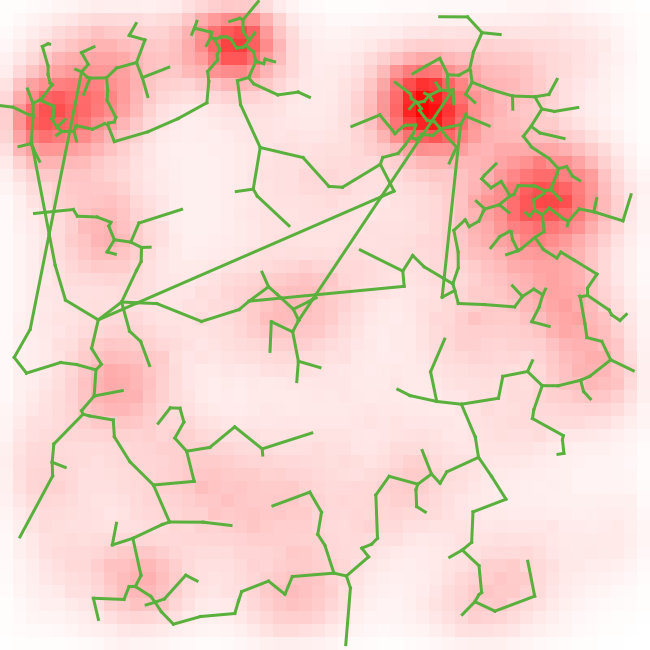
\includegraphics[width=\textwidth]{Figures/Cover/cover} \\ \vspace{3cm} % Picture

\mySubtitle \\ \medskip % Thesis subtitle
%Under the supervision of \myProf and \myOtherProf \\ \medskip
Sous la direction de \myProf et \myOtherProf \\ \medskip
%\myDegree \\
\myDepartment \\  \medskip
\myFaculty \\  \bigskip
%\myUni \\ \bigskip

\myTime\ -- \myVersion % Time and version

\vfill

\end{center}
\end{addmargin}

\end{titlepage} % Main title page

% Back of the title page

\thispagestyle{empty}

\hfill

\vfill

\noindent\myName: \textit{\myTitle,} \mySubtitle, %\myDegree, 
\textcopyright\ \myTime

% You may wish to do something with the back of the title page, such as including your supervisors, location or time frame of the work. Below is an example of doing so although you may want to tweak it to your liking.

%\bigskip

%\noindent\spacedlowsmallcaps{Supervisors}: \\
%\myProf \\
%\myOtherProf \\ 
%\mySupervisor

%\medskip \\

%\noindent\spacedlowsmallcaps{Location}: \\
%\myLocation

%\medskip \\

%\noindent\spacedlowsmallcaps{Time Frame}: \\
%\myTime
 % Back of the title page

\cleardoublepage% Dedication

\thispagestyle{empty}
\refstepcounter{dummy}

\pdfbookmark[1]{Dedication}{Dedication} % Bookmark name visible in a PDF viewer

\vspace*{3cm}



\bpar{
Our relation to our environment and people change at time scales we generally expect larger. Social relations are neither stationary nor in any kind of equilibrium at any time. They are chaos and complexity, as one's mind. As a witness, we include this preliminary dedication, for comparison purposes with the final version.
}{

}


%\begin{center}
%\emph{Ohana} means family. \\
%Family means nobody gets left behind, or forgotten. \\ \medskip
%--- Lilo \& Stitch    
%\end{center}
%
%\medskip
%
%\begin{center}
%Dedicated to the loving memory of Rudolf Miede. \\ \smallskip
%1939\,--\,2005
%\end{center} % Dedication page

\cleardoublepage% Abstract

%\renewcommand{\abstractname}{Abstract} % Uncomment to change the name of the abstract

\pdfbookmark[1]{Abstract}{Abstract} % Bookmark name visible in a PDF viewer

\begingroup
\let\clearpage\relax
\let\cleardoublepage\relax
\let\cleardoublepage\relax

\chapter*{Abstract}
%Short summary of the contents\dots a great guide by 
%Kent Beck how to write good abstracts can be found here:  
%\begin{center}
%\url{https://plg.uwaterloo.ca/~migod/research/beckOOPSLA.html}
%\end{center}


Territorial systems exhibit complexity at any levels and for most of their aspects. Related disciplines generally embrace complex systems science approaches to tackle their understanding and the associated dramatic social and environmental issues. Choosing a specific angle of lecture of territories, it appears, following territorial theories of networks, that real networks play a crucial role in system dynamics, and in particular transportation networks. Taking furthermore a modeling paradigm, we ask to what extent a modeling approach to territorial systems as networked human territories can help disentangling complexly involved processes. We propose to build an associated theory, relying on a vision of human territories as networked, combined with the evolutive urban theory and insights from morphogenesis and co-evolution, that we call a \emph{theory of co-evolutive networked territorial systems}. It is then embedded into a more general epistemological framework insisting on the notions of emergence and modularity. Quantitative epistemological analysis confirm the manual literature review and guide research towards co-evolutive models of networks and territories. We search for stylized facts in empirical datasets to also guide model construction. Methodological developments allow to expect information on dynamical processes from static correlations between urban morphology and network shape. The first modeling experiments include a calibrated spatial model of urban growth, giving an insight into theoretical assumption of network necessity. This model is then weakly coupled with a network generation heuristic to explore the space of feasible correlations. It paves the road for both comparison with real correlations and a strongly coupled calibrated model. We also explore novel paradigms such as the role of governance processes in network growth, through a game-theoretic agent-based model. These preliminary results provide the roadmap towards a family of comprehensive operational models of co-evolution between networks and territories that aim to disentangle their circular causalities.






\endgroup			

\vfill % Abstract page



\cleardoublepage
% Abstract

%\renewcommand{\abstractname}{Abstract} % Uncomment to change the name of the abstract

\pdfbookmark[1]{Reading Notes}{Reading Notes} % Bookmark name visible in a PDF viewer

\begingroup
\let\clearpage\relax
\let\cleardoublepage\relax
\let\cleardoublepage\relax

\chapter*{Reading Notes}

\textit{This provisory Memoire must be read as a work in progress, as it details progresses after one year of Doctorate. Many parts are given at the state of project, and not omitted as playing a role in the current research questioning. Its purpose is to set up a plan and examine the achieved work and corresponding directions, but also to share research ideas at this important step of one year.}




\endgroup			

\vfill



 % Uncomment and create a Foreword.tex to include a foreword



\cleardoublepage% Publications - a page listing research articles written using content in the thesis

\pdfbookmark[1]{Publications}{Publications} % Bookmark name visible in a PDF viewer

\chapter*{Publications} % Publications page text

%Some ideas and figures have appeared previously in the following publications:\\

%\noindent Put your publications from the thesis here. The packages \texttt{multibib} or \texttt{bibtopic} etc. can be used to handle multiple different bibliographies in your document.

%\begin{refsection}[ownpubs]
%    \small
%    \nocite{*} % is local to to the enclosing refsection
%    \printbibliography[heading=none]
%\end{refsection}

%\emph{Attention}: This requires a separate run of \texttt{bibtex} for your \texttt{refsection}, \eg, \texttt{ClassicThesis1-blx} for this file. You might also use \texttt{biber} as the backend for \texttt{biblatex}. See also \url{http://tex.stackexchange.com/questions/128196/problem-with-refsection}.

\bpar{
The following works have an highly overlapping content with this thesis:
}{
Les publications et communications suivantes contiennent la majorité du contenu de cette thèse. Les sources sont précisément mentionnées en introduction de chaque chapitre. Les traductions sont assurées par l'auteur le cas échéant.
}

% NOTE : on self-plagiarism, be careful to precise when extract from a published paper : 
%  - http://academia.stackexchange.com/questions/12342/self-plagiarism-in-phd-thesis
%  - http://academia.stackexchange.com/questions/2029/can-i-use-the-work-in-my-journal-conference-publications-as-chapters-in-my-disse
%  - http://academia.stackexchange.com/questions/149/what-is-a-sandwich-thesis


\section*{Publications}{Publications}


\noindent Raimbault, J. (2017). Identification of Causalities in Spatio-temporal Data, forthcoming in \textit{Sageo 2017 Proceedings.} arXiv:1709.08684

\bigskip

\noindent Raimbault, J. (2017). An Applied Knowledge Framework to Study Complex Systems, forthcoming in \textit{CSD\&M 2017 Proceedings.} arXiv:1706.09244


\bigskip

\noindent Raimbault, J. \& Bergeaud, A. (2017). The Cost of Transportation: Spatial Analysis of Fuel Prices in the US, forthcoming in \textit{Transportation Research Procedia, EWGT 2017.} arxiv:1706.07467


%\bigskip

%\noindent Antelope, C., Hubatsch, L., Raimbault, J., and Serna, J. M. (2016). An interdisciplinary approach to morphogenesis. Forthcoming in Proceedings of Santa Fe Institute CSSS 2016.

\bigskip

\noindent Bergeaud, A., Potiron, Y., \& Raimbault, J. (2017). Classifying patents based on their semantic content. \textit{PloS one, 12}(4), e0176310.

\bigskip

\noindent Raimbault, J. (2017). A Discrepancy-Based Framework to Compare Robustness Between Multi-attribute Evaluations. In \textit{Complex Systems Design \& Management} (pp. 141-154). Springer International Publishing. \cite{raimbault2017discrepancy}

\bigskip

\noindent Raimbault, J. (2017). Investigating the empirical existence of static user equilibrium. \textit{Transportation Research Procedia}, 22, 450-458. \cite{raimbault2017investigating}


\bigskip


\noindent Raimbault, J. (2016). Generation of Correlated Synthetic Data, forthcoming in \textit{Actes des Journ{\'e}es de Rochebrune 2016.}


\bigskip

\noindent Raimbault, J. (2015). Models Coupling Urban Growth and Transportation Network Growth: An Algorithmic Systematic Review Approach, forthcoming in \textit{ECTQG 2015 proceedings.} arxiv:1605.08888


\section*{Communications}{Communications}




\noindent Complexity, Complexities and Complex Knowledge, \textit{Geodivercity International Workshop, Paris, October 2017.}


\bigskip


\noindent Modeling the Co-evolution of Urban Form and Transportation Networks, \textit{Conference on Complex Systems 2017, Cancun, Sept. 2017.}

\bigskip

\noindent Raimbault J. \& Baffi S. (2017). Structural Segregation: Assessing the impact of South African Apartheid on Underlying Dynamics of Interactions between Networks and Territories, \textit{ECTQG 2017, York, Sept. 2017}


\bigskip


\noindent Invisible Bridges ? Scientific landscapes around similar objects studied from Economics and Geography perspectives, \textit{ECTQG 2017, York, Sept. 2017}


\bigskip


\noindent Cottineau C., Raimbault J., Le Texier M., Le N{\'e}chet F. \& Reuillon R. (2017). Initial spatial conditions in simulation models: the missing leg of sensitivity analyses?, \textit{Geocomputation 2017, Leeds, Sept. 2017}

\bigskip


\noindent A macro-scale model of co-evolution for cities and transportation networks, \textit{Medium International Conference, Guangzhou, June 2017}


\bigskip

\noindent Losavio C. \& Raimbault J. (2017). Agent-based Modeling of Migrant Workers Residential Dynamics within a Mega-city Region: the Case of Pearl River Delta, China, \textit{Urban China Development International Conference, London, May 2017}


\bigskip

\noindent Co-construire Modèles, Etudes Empiriques et Théories en Géographie Théorique et Quantitative: le cas des Interactions entre Réseaux et Territoires. In \textit{Treizièmes Rencontres de ThéoQuant, Besançon, Mai 2017}


\bigskip

\noindent Un Cadre de Connaissances pour une Géographie Intégrée. In \textit{Journée des jeunes chercheurs de l'Institut de Géographie de Paris, Paris, April 2017}


\bigskip


\noindent Towards a Theory of Co-evolutive Networked Territorial Systems: Insights from Transportation Governance Modeling in Pearl River Delta, China, \textit{MEDIUM Seminar : Sustainable Development in Zhuhai, Guangzhou, Dec 2016.}


\bigskip


\noindent Models of growth for system of cities : Back to the simple, \textit{Conference on Complex Systems 2016, Amsterdam, Sep 2016.}



%Raimbault J., Bergeaud A. and Potiron Y. (2016). Investigating Patterns of Technological Innovation. \textit{Conference on Complex Systems 2016, Amsterdam, Sep 2016.}


\bigskip

\noindent For a Cautious Use of Big Data and Computation. \textit{Royal Geographical Society - Annual Conference 2016 - Session : Geocomputation, the Next 20 Years (1), London, Aug 2016.}


\bigskip

\noindent Indirect Bibliometrics by Complex Network Analysis. \textit{20e Anniversaire de Cybergeo, Paris, May 2016.}


\bigskip

\noindent Raimbault, J. \& Serra, H. (2016). Game-based Tools as Media to Transmit Freshwater Ecology Concepts, \textit{poster corner at SETAC 2016 (Nantes, May 2016).}


\bigskip

\noindent Le Néchet, F. \& Raimbault, J. (2015). Modeling the emergence of metropolitan transport authority in a polycentric urban region, \textit{ECTQG 2015, Bari, Sep 2015).}


\bigskip

\noindent Hybrid Modeling of a Bike-Sharing Transportation System, \textit{poster presented at ICCSS 2015, Helsinki, June 2015.}

\bigskip

\noindent Raimbault, J. \& Gonzales, J. (2015). Application de la Morphog{\'e}n{\`e}se de R{\'e}seaux Biologiques {\`a} la Conception Optimale d'Infrastructures de Transport, \textit{poster presented at Rencontres du Labex Dynamite, Paris, May 2015.}


 % Publications from the thesis page

\cleardoublepage% Acknowledgements

\pdfbookmark[1]{Acknowledgements}{Acknowledgements} % Bookmark name visible in a PDF viewer

\begin{flushright}{\slshape    
We have seen that computer programming is an art, \\ 
because it applies accumulated knowledge to the world, \\ 
because it requires skill and ingenuity, and especially \\
because it produces objects of beauty.} \\ \medskip
--- \defcitealias{knuth:1974}{Donald E. Knuth}\citetalias{knuth:1974} \citep{knuth:1974}
\end{flushright}

\bigskip

%----------------------------------------------------------------------------------------

\begingroup

\let\clearpage\relax
\let\cleardoublepage\relax
\let\cleardoublepage\relax

\chapter*{Acknowledgements}

\noindent Put your acknowledgements here.\\

\noindent Many thanks to everybody who already sent me a postcard!\\

\noindent Regarding the typography and other help, many thanks go to Marco Kuhlmann, Philipp Lehman, Lothar Schlesier, Jim Young, Lorenzo Pantieri and Enrico Gregorio\footnote{Members of GuIT (Gruppo Italiano Utilizzatori di \TeX\ e \LaTeX )}, J\"org Sommer, Joachim K\"ostler, Daniel Gottschlag, Denis Aydin, Paride Legovini, Steffen Prochnow, Nicolas Repp, Hinrich Harms, Roland Winkler, and the whole \LaTeX-community for support, ideas and some great software.

\bigskip

\noindent\emph{Regarding \mLyX}: The \mLyX\ port was initially done by
\emph{Nicholas Mariette} in March 2009 and continued by
\emph{Ivo Pletikosi\'c} in 2011. Thank you very much for your work and the contributions to the original style.

\endgroup % Acknowledgements page

\pagestyle{scrheadings} % Show chapter titles as headings

\cleardoublepage% Table of Contents - List of Tables/Figures/Listings and Acronyms

\refstepcounter{dummy}

\pdfbookmark[1]{\contentsname}{tableofcontents} % Bookmark name visible in a PDF viewer

\setcounter{tocdepth}{1} % Depth of sections to include in the table of contents - currently up to subsections

\setcounter{secnumdepth}{2} % Depth of sections to number in the text itself - currently up to subsubsections

\manualmark
\markboth{\spacedlowsmallcaps{\contentsname}}{\spacedlowsmallcaps{\contentsname}}
\tableofcontents 
\automark[section]{chapter}
\renewcommand{\chaptermark}[1]{\markboth{\spacedlowsmallcaps{#1}}{\spacedlowsmallcaps{#1}}}
\renewcommand{\sectionmark}[1]{\markright{\thesection\enspace\spacedlowsmallcaps{#1}}}

\clearpage

\begingroup 
\let\clearpage\relax
\let\cleardoublepage\relax
\let\cleardoublepage\relax

%----------------------------------------------------------------------------------------
%	List of Figures
%----------------------------------------------------------------------------------------

\refstepcounter{dummy}
%\addcontentsline{toc}{chapter}{\listfigurename} % Uncomment if you would like the list of figures to appear in the table of contents
\pdfbookmark[1]{\listfigurename}{lof} % Bookmark name visible in a PDF viewer

\listoffigures

\vspace{8ex}
%\newpage

%----------------------------------------------------------------------------------------
%	List of Tables
%----------------------------------------------------------------------------------------

\refstepcounter{dummy}
%\addcontentsline{toc}{chapter}{\listtablename} % Uncomment if you would like the list of tables to appear in the table of contents
\pdfbookmark[1]{\listtablename}{lot} % Bookmark name visible in a PDF viewer

%\chapter*{List of Tables}

\phantomsection

\listoftables
        
\vspace{8ex}
\newpage
    
%----------------------------------------------------------------------------------------
%	List of Listings
%---------------------------------------------------------------------------------------- 

%\refstepcounter{dummy}
%\addcontentsline{toc}{chapter}{\lstlistlistingname} % Uncomment if you would like the list of listings to appear in the table of contents
%\pdfbookmark[1]{\lstlistlistingname}{lol} % Bookmark name visible in a PDF viewer

%\lstlistoflistings 

%\vspace{8ex}
%\newpage
       
%----------------------------------------------------------------------------------------
%	Acronyms
%----------------------------------------------------------------------------------------

%\refstepcounter{dummy}
%\addcontentsline{toc}{chapter}{Acronyms} % Uncomment if you would like the acronyms to appear in the table of contents
%\pdfbookmark[1]{Acronyms}{acronyms} % Bookmark name visible in a PDF viewer

%\markboth{\spacedlowsmallcaps{Acronyms}}{\spacedlowsmallcaps{Acronyms}}

%\chapter*{Acronyms}

%\begin{acronym}[ABM]
%\acro{ABM}{Agent-based Modeling}
%\acro{API}{Application Programming Interface}
%\acro{UML}{Unified Modeling Language}
%\end{acronym}  
             
             

%\begin{acronym}[SOC]
%\acro{ABM}{Self-organized Criticality}
%\end{acronym} 
             
             
             
                   
\endgroup % Contents, list of figures/tables/listings and acronyms

\cleardoublepage

\pagenumbering{arabic} % Arabic page numbering for thesis content (1, 2, 3, etc)
%\setcounter{page}{90} % Uncomment to manually start the page counter at an arbitrary value (for example if you wish to count the pre-content pages in the page count)

\cleardoublepage % Avoids problems with pdfbookmark

%----------------------------------------------------------------------------------------
%	THESIS CONTENT - CHAPTERS
%----------------------------------------------------------------------------------------






%%%%%%%%%%%%%%%%%%%%
%% Organisation and general points



\comment{(Florent) cf receuil articles du Monde sur Grd Paris (numériser)}

\comment{(Florent) HDR Anne ?}


\comment{(Florent) trop peu ancré concrètement dans le champ des interactions transport/ville - enchainement idée ok mais revoir granularité info. Catalogue de situations complexes d'interactions forme urbaine/transport à reproduire.}



\comment{(Arnaud) Sur le plan : Contexte ; Théorique ; cadre Methodo. Quant epistemo avant methodo ou théorie ? Publier Cybergeo ; Article ectqg en annexe ; dans méthodo : ajouter Modèle agents - hors équilibre  ; reorg Empirical etc (Q/T)}


\comment{(Arnaud) A LIRE : R Brunet, Discontinuités en géographie ; Pierre Dumolard (Espace Différencié) ; Guy DiMeo (L'homme, la société, l'espace)}







%%%%%%%%%%%%%%%%%%%%
% TODO - todo
%
% -- TODO --

% - checker redondances bibliographie, et exactitude des records, publications arxiv, etc. !! biblio des appendices dans la générale ? a voir.
% - inclure éthique de la connaissance de Monod.
% - why not include artwork as appendix. science<->art (// poésies ?)
% - appendix : ecogeo - include results and discussions ; idem conf Medium ?
% - Morphogenesis : * reclarify link between dynamics and form in Thom's theory ; * find time to do quant epistemo ; * on the definition of the system and boundaries : missing part ?
% - somewhere clarification and discussion on definitions of emergence, Bedau etc. ? done on several points.
% - sur multi-scale modeling : who does some and how much ? à ajouter quelque part
% - pour la PDE : voir Villani, mentionner ?
% - effective dimension of urban system : sens ? (comment density) : question assez profonde à méditer - lié info sémantique portugali ? lié représentation minimale ?
% - on density multi-scale dvlpmt : pas clair ce que tu as en tête ici : je ne sais pas si tu auras le temps de creuser cela, mais pour du multi-scalaire, les schémas sont très aidant car c'est vite difficile à visualiser
% - morphogénétiques : est-ce que le mot existe, orthographe pas logique !
% - correlated synthetic data : appendix : inclure regressions
% - revoir discussion correlated synthetic data


%% -- DONE --
%
%  X - attention aspect uniformisateur/limite totalitariste vision sci ? -> ok clarifier avec anarchisme et Feyerabend.
%  X - trouver un moyen d'élargir systématiquement toutes les figures ?

%%%%%%%%%%%%%%%%%%%%
% TODO - include notes

% -> notes.md




%%%%%%%%%%%%%%%%%%%%
% TODO - Reading Records
%
%% -- A LIRE -- 

% - lire Morin sur la pensée complexe
% - Moore Nature of Computation

%% -- A INCLURE --
%



%%%%%%%%%%%%%%%%%%%%
% TODO - Ideas

% - cours : la ville est la combinaison de forces opposées, souvent contradictoire. (cours analyse spatiale). far-from-equilibrium of course.

%  -- URGENT -- (when writing comments on network growth models) : do a sort of list of processes, implied objects, etc. / or a tab , from modeling, theories and CASES STUDIES --


% -  companion site à la Seb ?

% -  a note on open review via git ?



%%%%%%%%%%%%%%%%%%%%
% TODO - Citations
%
% -> potential citations

%  - Le sérieux n'est que la crasse accumulée dans les têtes vides - Roland Topor

%  - Science is an essentially anarchic enterprise - Paul Feyerabend, Against Method

%\headercit{Mais ce n'est pas une question d'{\^a}ge, de chiffres et de stats\\ Moi je te parle surtout de rage, de kif et d'espoir}{Youssoupha}{\textit{, Esperance de Vie}}

% %\headercit{Do or do not. There is no try.}{Yoda}{}


%%%%
% voie de garage

%  - % The Social Construction of What ?}{Ian Hacking}{\cite{hacking1999social} -> pas vraiment une citation, et pas adapté à grand chose..
 
%\headercit{Your theory is crazy, but not enough to be true.\comment{(Florent) rigolo mais le rapport avec le sujet est discutable}}{Niels Bohr}{}





%%%%%%%%%%%%%%%%%%%%
% TODO - Uncited
%
% -> uncited refs, why.
%
%2017arXiv170108673P -> number of states of HMM : ?
%levy1993t -> Levy theory on territory : need a deeper read and connections.
%pumain2017geography
%batty2017cities
%2017arXiv170107861D
%nicosia2009extending
%10.1371/journal.pone.0170830
%varma2017hpc
%Munafo:2017uq
%railsback2017
%2017arXiv170102973L
%2017arXiv170102383G
%shashok2017can
%miandoabchi2013multi
%farahani2013review
%fujita1982multiple
%bitbol2004autopoiesis
%dollens2014alan
%Chavalarias2016
%2016arXiv161208111S
%2016arXiv161208338T
%friesz1985transportation
%sui2004tobler
%miller2004tobler
%tobler2004first : Tobler giving precisions on the first law of geography
%2016arXiv161205463G
%raimbault2016discrepancy
%raimbault2016investigating
%2016arXiv161102269V
%2015arXiv150402550T
%batty2005agents
%xue2006spatial
%shen2002urban
%xu2005city
%10.1371/journal.pone.0166011
%10.1371/journal.pone.0166004
%2016arXiv161103232L
%hou2011transport
%cao2012accessibility
%huang2016association
%10.1371/journal.pone.0164553
%chan2005location
%tardy2004role
%perret2015roads
%makse1995modelling
%2016arXiv160904636V
%clauset2004finding
%2016arXiv160902000G
%2016arXiv160808839C
%Downey30082016
%osmosis
%xie2009topological
%rozenfeld2008laws
%2016arXiv160805770C
%2016arXiv160806313S
%2016arXiv160806897H
%2015arXiv151207603T
%duranton2007urban
%dimeo2016geographie
%2016arXiv160608103M
%raimbault2016generation
%raimbault2015hybrid
%raimbault2015user
%raimbault2016system
%swerts2013systemes
%swerts2015megacities
%florida2008rise
%hall1982great
%2016arXiv160805266R
%aveline2016medium
%lenechet:halshs-01272236
%2016arXiv160804472J
%ioannidis2005most
%2016arXiv160803608M
%batty2007creative
%chen2012wider
%hall1997modelling
%knowles2016sir
%reid2016decision
%carreira2000mode
%yu2012solving
%wang2015resilience
%masucci2014exploring
%fessel2012physarum
%gaughan2016spatiotemporal
%raimbault2016simpopsan
%10.1371/journal.pone.0160471
%10.1371/journal.pone.0159496
%pan2003croissance
%2016arXiv160708472M
%lyu2016developing
%emangard2009transports
%e18060197
%ishiguro1997bootstrapping
%Woodhouse19072016
%10.1371/journal.pone.0158826
%10.1371/journal.pcbi.1004947
%2016arXiv160703186A
%10.1371/journal.pone.0157261
%saichev2009theory
%karrer2011stochastic
%gastner2006shape
%10.1371/journal.pone.0157728
%2015arXiv150607608T
%2016arXiv160601959F
%sornette1997convergent
%solomon1996spontaneous
%gabaix2003theory
%newling1966urban
%bretagnolle2000long
%pumain2006villes
%okabe1987theoretical
%dellaposta2016endogenous
%Squartini:2013fk
%Takeuchi20153109
%2016arXiv160501949B
%klimek2012empirical
%10.1371/journal.pone.0154839
%2016arXiv160408816Z
%2016arXiv160407876G
%jiang2007topological
%akaike1998information
%heiss2008likelihood
%2005physics..12106P
%hall1990methodology
%burnham2004multimodel
%manning2014stanford
%thom1974stabilite
%benguigui1991suburban
%durand1990notion
%batty1991generating
%dauphine1995chaos
%dupuy:halshs-00438867
%damm1980response
%coffman1998railroad
%knight1977evidence
%goldberg1972evaluation
%alcaly1976transportation
%aveline2003ville
%2016arXiv160402872L
%2016arXiv160400758D
%2016arXiv160404155A
%2016arXiv160403904B
%2015arXiv151104268L
%echenique2012growing
%Brunton12042016
%banos2011christaller
%10.1371/journal.pone.0152686
%dupuy1993geographie
%newman1996land
%kenworthy2002transport
%tirnakli2015standard
%benettin1980lyapunov
%hijmans2015geographic
%10.1371/journal.pone.0151676
%offner2000territorial
%bourgine2010morphogenesis
%Fujita199693
%lenormand2015comparing
%soler2014calculating
%gallotti2015transportation
%krugman1998space
%lenormand2012generating
%decraene2013emergence
%varenne2008epistemologie
%derrible2010complexity
%10.1371/journal.pone.0150932
%10.1371/journal.pone.0148660
%le2015modeling
%mehaffy2007notes
%cuyala2013diffusion
%ciotti2015homophily
%el2006access
%2015arXiv151003797G
%2016arXiv160208451P
%choi2014patent
%shibata2008detecting
%zembri2010new
%2015arXiv150901940M
%schmid1994probabilistic
%noruzi2005google
%bohannon2014scientific
%2015arXiv150601280B
%2016arXiv160106075O
%10.1371/journal.pone.0147913
%barthelemy2015time
%raffestin1982remarques
%Gao:2016ty
%fujita1996economics
%2016arXiv160203774H
%blondel2008fast
%min2011real
%schultz2014random
%jedwab2013transportation
%offner2002x
%bitner2009complex
%raimbault2015models
%2015arXiv151205659M
%achlioptas2009explosive
%10.1371/journal.pone.0146491
%2015arXiv151207715C
%2015arXiv151205259R
%2015arXiv151200946S
%2015arXiv151201423W
%di1998espace
%2015arXiv151105468E
%2014arXiv1403.3005S
%Brummitt20150712
%beckman1996creating
%simini2012universal
%masucci2013gravity
%witten1981diffusion
%kuhnert2006scaling
%aghion2002schumpeterian
%andersson2002urban
%frankhauser1998fractal
%2015arXiv151006326H
%Sinatra:2015yu
%su2008effect
%fraedrich1986estimating
%chen2009spatial
%2015arXiv150909055P
%Perret:2015fk
%2015arXiv150907599C
%2015arXiv150803542B
%pumain2006hierarchy
%vattay2015quantum
%2014arXiv1403.7686B
%2015arXiv150904486M
%2015arXiv150903678R
%2015arXiv150905183R
%2015arXiv150905590H
%2015arXiv150904558J
%Pohlert:2015fk
%cheng2004notes
%cristelli2012there
%fox2005revisiting
%newman2005power
%clauset2009power
%kyriakidou2011applying
%bretagnolle:halshs-00159894
%sanders2006artificial
%courbaud2015applying
%2015arXiv150707878C
%10.1371/journal.pone.0133780
%gilli2005bassin
%servais2004polycentrisme
%leveque:halshs-00280396
%urbanek2011emdist
%wikle1999dimension
%galka2004solution
%vitanov2015test
%hens2015extreme
%2015arXiv150507372L
%pan2013urban
%tretyakov2011fast
%pumain2004urban
%Capozza1990187
%thevenin2013mapping
%schwartz2011spatial
%roth2012long
%10.1371/journal.pone.0029721
%Ye2014200
%donaldson2010railroads
%lucas1998mechanics
%moretti2004human
%banos2012network
%gauvin2009phase
%chen2010characterizing
%kang2012intra
%Karatzoglou:2004uq
%R-Core-Team:2015fk
%anderson1991turning
%underhill1990soviet
%baklanov2015projects
%perret2010multi
%crucitti2006centrality
%frankhauser2008fractal
%pumain1998urban
%Schwarz201029
%hebert2011structural
%batty2006hierarchy
%lugovoy2007analysis
%dorogovtsev2000structure
%pumain2002role : epistemology on TQG
%Mandelbrot1961198
%Mandelbrot195990
%bailey1999funk
%roopkumar2006generalized
%pumain2015multilevel
%reuillon2015
%10.1371/journal.pcbi.1004101
%anas1998urban
%ribeiro2010game
%Roumboutsos2008209
%le2010approche
%ordeshook1986game
%lenechet:halshs-00674059
%lenechet2012
%keitt2011rgdal
%baddeley2004spatstat
%gallego2010population
%hirtzel:tel-01121665
%martin2004generating
%abadie2011synth
%coulombel:tel-00601262
%strano2012elementary
%networkQgis
%mills2000thematic
%fujita2004new
%cookbookForR
%leurent2012disaggregate
%fields1999city
%dori2002object
%zeigler1989devs
%louail:tel-00584495
%goldspink2000modelling
%Liu201326
%lechner2006procedural
%parish2001procedural
%beauguitte2014r
%andersson2003urban
%brown2005spatial
%Magliocca2011183
%Ettema20111
%phan2010agent
%clarke1998loose
%He2006323
%kocabas2006coupling
%Kunz2000597
%zanette1997role
%clarke2007decade
%achibetmorphogenese
%rui2013urban
%lodin2011road
%porta2006network
%andersson2006complex
%eboli2012exploring
%duranton2012urban
%horner2012analyzing
%2013PhRvL.111s8702L
%antoni:hal-00914269
%berroir2005contribution
%guerois2002commune
%hall2006polycentric
%offner:halshs-00438903
%portugali2012complexity
%
%

% X biernacki2000assessing -> empirical likelihood (paper interactionGibrat)
% X bon2017novel -> SJS
% X bettencourt2007growth : Bettencourt scaling theory of cities
% X bourgine2010morphogenesis : in morphogenesis
% X loo1999development : planning transportation in DPR
% X favaro2007croissance : thèse JM Favaro
% X paulus2004coevolution : specialisation of urban areas











%----------------------------------------------------------------------------------------



%%%%%%%%%%%%%%%%%%%%%%%%%%%%%
% Introduction
%
\ctparttext{}
%
\part*{Introduction}
%



%%%%%%%%%%%%%%%%
%%  Introduction
%%%%%%%%%%%%%%%%


%% Contents
%
%    - General considerations on Complex Systems, positioning etc (thesis in cs science etc)
%    - Thematic introduction, geographical introduction of the subject.
%
%   - precisions on v1 memoire : foreword ?
%
%    - reading precisions : organisation, interdependances etc 
%
%   - reflexive aspect : here ?  


\chapter*{Introduction}

% to have header for non-numbered introduction
\markboth{Introduction}{Introduction}

%\headercit{We need to find Banos' tenth modeling law}{Ren{\'e} Doursat}{}
\headercit{It's when you shuffle the anthill that you get a touch of all its complexity.}{Arnaud Banos}{}

% citation self-consistent ? -> seems ok

\bigskip


``In consequence of a technical issue, traffic is interrupted on the line B of RER, for an unknown duration. More information will be given as soon as available''. There is a high probability that someone having lived or spent some time in the metropolitan region of Paris has already heard this frightening announce and endured the difficult consequences the rest of his day. But he might not be aware of the ramifications of causal cascades induced by this not-so-rare event. Territorial Systems, whatever the layers considered in their definitions, will always be extremely complex and interrelations at numerous temporal and spatial scales participate in the emergent behaviors observed at any levels of the system. Martin is a student who daily commutes from Paris to Palaiseau and will miss today a crucial exam, what will have a profound impact on his professional life : implications at a long time scale, small spatial scale and agent granularity. Yuangsi is connecting Orly and Roissy Airports, in his trip from London to Beijing, will miss his plane and his sister's wedding : large spatial scale, short time scale, agent granularity. A collective petition emerges from users, leading to new social organizational patterns and reaction from transportation authority that results in efforts to increase levels of service : mesoscopic temporal and spatial scale, swarm of agents granularity. Looking for causes of the event will also lead to intricate processes at various scales, none of which seems to be a better explication than others : historical railway network in Parisian region shaped further extensions and RER B followed the former \textit{Ligne de Sceaux}, \noun{Delouvrier}'s schema for regional development, and its subsequent partial execution, are elements of explanation of structural weaknesses of Parisian public transportation network~\cite{gleyze2005vulnerabilite} ; commuting patterns consequent to territorial organisation induce an overload of particular lines and thus a necessary increase in exploitation incidents. The list could be developed much longer and each approach related to an already mature scientific body of knowledge in different disciplines such as geography, urban economics, transportation. This amusing anecdote is enough to give a touch of the complexity of territorial systems. Our aim here is to dive into this complexity, and in particular to give an original insight into the study of relations between networks and territories. The choice of this reading position will be largely discussed in a further thematic part. Let for now concentrate on the originality of the point of view that we will take.



%-------------------------------------------------

\section*{Scientific Context : Complexity Has Come of Age}


To better introduce our subject, it is necessary to make the reader aware of the particular scientific context we are working in. It is necessary both to understand the general epistemology underlying research questions, and to be aware of the variety of methods and tools used. Contemporaneous science is progressively taking the shift of complexity in many fields. That also implies an epistemological revolution to abandon strict reductionism that failed in most of its synthesis attempts~\cite{anderson1972more}. Arthur recently recalled~\cite{arthur2015complexity} that a mutation of methods and paradigms was also at stake by the increasing role of computational approaches replacing purely analytical techniques generally self-limited in their modeling and resolution scope. Capturing \emph{emergent properties} in models of complex systems is one of the ways to understand the essence of these new approaches.

These considerations are well known in Social Science (both quantitative and qualitative), in which the complexity of studied agents and systems is the justification of their existence : if humans were particles a whole branch of fields may have never emerged as thermodynamics would have solved most of social issues. \footnote{even if it would probably not have been the case as classical physics also failed in their attempts to include irreversibility and evolutions of Complex Adaptive Systems as Prigogine points out in \cite{prigogine1997end}} 
They are however less known nor accepted in more ``hard'' sciences such as physics : Laughlin develops in~\cite{laughlin2006different} a view of the discipline at least as at a ``frontier of knowledge'' then other fields appearing as less mature. Most of knowledge is of classical nature although a majority of structures and systems would be \emph{self-organized}, what means that the single microscopic laws are not enough to determine macroscopic properties unless system evolution is simulated (more precisely this property can be taken as a definition of emergence on which we will come back further, and self-organization is intrinsically emergent). It corresponds to the first nightmare of Laplace's Deamon developed in~\cite{deffuant2015visions}.


As an informal mix of epistemological positions, methods, and fields of applications, \emph{Complexity Science} relies on typical paradigms such as the centrality of emergence and self-organization in most of phenomena of the real world, which make it lie on a frontier of knowledge closer of us than we can think (Laughlin, op.cit. ). Such concepts are indeed not new, as they were already enlighten by Anderson~\cite{anderson1972more}. Even cybernetics can be related to complexity by seing it as a bridge between technology and cognitive science~\cite{wiener1948cybernetics}. Later, synergetics~\cite{haken1980synergetics} paved the way for a theoretical approach of collective phenomena in physics. Reasons for the recent growth of works claiming a CS approach may be various. The explosion of computing power is surely one because of the central role of numerical simulations~\cite{varenne2010simulations}. They could also be the related epistemological progresses : apparition of the notion of perspectivism~\cite{giere2010scientific}, finer reflexions around the notion of model~\cite{varenne2013modeliser}\footnote{In that frame scientific and epistemological progress can not be dissociated and can be seen as coevolving}. The theoretical and empirical potentialities of such approaches play surely a role in their success\footnote{
Although the adoption of new scientific practices may be strongly biased by imitation and lack of originality~\cite{dirk1999measure}, or more ambivalent, by marketing strategies as the fight for funds is becoming a huge obstacle for research~\cite{bollen2014funding}.}, as confirmed in various domains of application (see~\cite{newman2011complex} for a general survey), as for example Network Science~\cite{barabasi2002linked} ; Neuroscience~\cite{koch1999complexity}; Social Sciences ; Geography~\cite{manson2001simplifying}\cite{pumain1997pour} ; Finance with the rising importance of econophysics~\cite{stanley1999econophysics} ; Ecology~\cite{grimm2005pattern}. The Complex Systems Roadmap~\cite{2009arXiv0907.2221B} proposed a double lecture of studies on Complex Systems : an horizontal approach connecting fields of study with transversal questions on theoretical foundations of complexity and empirical common stylized facts, and a vertical conceptions of disciplines, with the aim to construct integrated disciplines and corresponding multi-scale heterogeneous models. Interdisciplinarity is thus central in our scientific background.



\section*{Interdisciplinarity}

%\textit{Note : that term does not exist in english but is a rough translation from french \emph{interdisciplinarit{\'e}}, that we believe to better express }
%
%
%WHY and HOW is interdisciplinarity essential ?
%
% Q : quote Morin ?
%


We must further insist on the role of interdisciplinarity in the positions taken here. This is not a thesis in Geography nor in Complex Adaptive Systems Modeling, but in \emph{Complex Systems Science} that we claim as a proper discipline following \noun{Paul Bourgine}. It will naturally be seen with defiance by scholars of various concerned disciplines, as recent examples of misunderstandings and conflicts have illustrated~\cite{dupuy2015sciences}. The positioning of \noun{Batty} proposing \textit{A new Science of Cities}~\cite{batty2013new} (that he subtly presents as \textit{The} new science of cities) is directed towards an integration of disciplines and methods into a science defined by its object of study, cities. Its theoretical and epistemological weaknesses (no theoretical constructions of studied geographical objects on the one hand, approximative contextualization of complexity) combined with an overall impression of \emph{pot-pourri} of forgotten works (space syntax, land-use models), unfortunately avoid us to use it as we will use geographical theories (e.g. evolutive urban theory) in an appropriated epistemological complexity context. Yet our reading of this work may be the result of a misunderstanding due to different cultural backgrounds.


%\subsection*{Conflicting Complexities and Cultural Differences}

The scientific evolution of complexity that some see as a revolution~\cite{colander2003complexity}, or even as \emph{a new kind of science}~\cite{wolfram2002new}, could indeed face intrinsic difficulties due to behaviors and a-priori of researchers as human beings. More precisely, the need of interdisciplinarity that makes the strength of Complexity Science may be one of its greatest weaknesses, since the highly partitioned structure of science organization has sometimes negative impacts on works involving different disciplines. We do not tackle the issue of over-publication, competition, indexes, which is more linked to a question of open science and its ethics, also of high importance but of an other nature. That barrier we are dealing with and we might struggle to triumph of, is the impact of certains \emph{cultural disciplinary differences} and out-coming conflicts on views and approaches. 
The drama of scientific misunderstandings is that they can indeed annihilate progresses by interpreting as a falsification some work that answers to a totally different question. The example of a recent work on top-income inequalities given in~\cite{aghion2015innovation}, which conclusions are presented as opposed from the one obtained by Piketty~\cite{piketty2013capital}, follows such a scheme. Whereas Piketty focused on constructing long-time clean databases for income data and showed empirically a recent acceleration of income inequalities, his simple model aiming to link this stylized fact with the accumulation of capital has been criticized as oversimplified. On the other hand, Bergeaud \textit{et al.} prove by a model of innovation economics that \emph{under certain assumptions} income gaps may be beneficial to innovation and consequently a general utility. Thus diverging conclusions about the role of personal capitals in the economy. But diverging \emph{views} or \emph{interpretations} does not mean a scientific incompatibility, and one could imagine try to gather both approaches in an unified framework and model, yielding possibly similar or different interpretations. This integrated approach has chances to contain more information (depending on how coupling is done) and to be a further advance in Science. We shall now briefly develop other examples to give an overview how conflicts between disciplines can be damaging.


\paragraph{Physics reinvents geography.}

As already mentioned, \noun{Dupuy} and \noun{Benguigui} points out in \cite{dupuy2015sciences} the fact that urban sciences have recently known open conflicts between old tenants of the disciplines and new arrivants, especially physicists. The availability of large datasets of new type of data (social networks, ICT data) have drawn their attention towards the study of objects traditionally studied by human science, as analytical and computational methods of statistical physics became applicable. Although these studies are generally presented as the construction of a scientific approach to cities, implying that existing knowledge was not scientific because of their more qualitative aspect, they have not unveil specifically novel knowledge on urban systems : to give some examples, \cite{barthelemy2013self} concludes that Paris has followed a transition during Haussman period and that the evolution of a city is the combination of local transformations and global planning operations, what are facts known for a long time in urban history and urban geography. \cite{chen2009urban} rediscovers that the gravity model can be improved by adding lags in interactions and theoretically derives the expression of the force of interaction between cities, without any thematic theoretical background. Examples could be multiplied, confirming the current discomfort in communication between physicists and urban geographers. Significant benefices could results from a wise integration of disciplines~\cite{o2015physicists} but the road seems still long.

\paragraph{Economic Geography or Geographical Economics ?}

Similar conflict occurred in economics : as \cite{marchionni2004geographical} describes, the discipline of economic geography, traditionally close from geography, heavily criticized a new stream of thought named \emph{geographical economics}, which purposes is spatialization of mainstream economic techniques. Both do not have the same purposes and aims, and the conflict appears as a total misunderstanding for an external observer.


\paragraph{Agent-based Modeling in Economy}

Disciplinary conflicts may also manifest themselves as the reject of novel methods by mainstream currents. Following \cite{farmer2009economy}, the operational failure of most classic economic approaches could be compensated by a broader use of agent-based modeling and simulation practices. The lack of analytical framework that is natural in the study of complex adaptive systems seems to be rebutting for most of economists.


\paragraph{Finance}

In Quantitative Finance coexist various stream of research with a very few interactions. Let consider two examples. On the one hand, Statistics are highly advanced in theoretical mathematics, using stochastic calculus and probabilities to obtain very refined estimators of parameters for a given model (see e.g. \cite{barndorff2011multivariate}). On the other hand, Econophysics aims to study empirical stylized facts and infer empirical laws to explain complexity-related phenomena in financial systems~\cite{stanley1999econophysics}, such as e.g. cascades leading to market crashes, fractal properties of asset signals, complex structure of correlation networks. Both have their advantages in a particular context and each would benefit from increased interactions between the fields.


\bigskip

These diverse examples illustrate how interdisciplinarity is both crucial and difficult to achieve. We will try to follow that narrow path in our work, borrowing ideas, theories and methods from various disciplines, aiming for the construction of an integrated knowledge. Indeed, coupling heterogeneous approaches at different levels and scales will be a cornerstone of our thesis, skeleton of the underlying philosophy and building brick of the theory we will propose.







%-------------------------------------------------

\section*{Complexity in Geography}


Coming back to our introducing anecdote, we will focus on our thematic object of study that are territorial systems. More generally, we propose an overview of the role of complexity in geography. Geographers are familiar with complexity for a long time, as the study of spatial interactions is one of its purposes. The variety of fields in geography (geomorphology, physical geography, environmental geography, human geography, health geography to give a few) has certainly been important in the subtlety of the geographical thinking, that considers heterogeneous and multi-scalar processes.

\noun{Pumain} recalls in~\cite{pumain2003approche} a subjective history of the emergence of complexity paradigms in geography. Cybernetics yielded system theories as the one developed by Forrester. Later the shift to self-organized criticality and self-organisation concepts in physics conducted to corresponding developments in geography, as \cite{sanders1992systeme} witnesses the application of the concepts of synergetics for the dynamics of an urban system. Finally, Complex Systems paradigms as we currently know them appeared from various points of view. For example, the fractal nature of urban shape was introduced in~\cite{batty1994fractal} and had numerous application including more recent developments~\cite{keersmaecker2003using}. \noun{Batty} also introduced cellular automata in urban modeling and proposed a joint synthesis with agent-based modeling and fractals in~\cite{batty2007cities}. An other incursion of complexity in geography was for the case of urban systems through the evolutive urban theory of \noun{Pumain}. In close relation with modeling from the beginning (the first Simpop model described in~\cite{sanders1997simpop} enters the theoretical framework of \cite{pumain1997pour}), this theory aims to understand system of cities as systems of co-evolving adaptive agents, interacting in many ways, with particular features emphasized such as the diffusion of innovation. The series of Simpop models~\cite{pumain2012multi} focused in testing various assumptions of the theory. For example, different underlying mechanisms were revealed for european city systems and city system of the united states~\cite{bretagnolle2010comparer}. At other time scales and in other contexts, the SimpopLocal model~\cite{schmitt2014modelisation} aimed to investigate the conditions for the emergence of hierarchical urban systems from disparate settlements. A minimal model (in the sense of sufficient and necessary parameter) has been isolated thanks to the use of intensive computation with the model exploration software OpenMole~\cite{schmitt2014half}, what was a result analytically not derivable for this kind of complex model. The technical progresses of OpenMole~\cite{reuillon2013openmole} were done simultaneously with theoretical and empirical advancements. Epistemological advances were also essential to this framework, as \noun{Rey} develops in~\cite{rey2015plateforme}, and novel concepts such as incremental modeling~\cite{cottineau2015incremental} were found, with powerful concrete applications : \cite{cottineau2014evolution} implemented it on the soviet city system and isolated dominating socio-economic processes, by systematic testing of thematic assumptions and implementation functions. Directions for the development of such Modeling and Simulation practices in quantitative geography were recently introduced by \noun{Banos} in~\cite{banos2013pour}. He concludes with nine principles\footnote{I remember \noun{Ren{\'e} Doursat} insisting on the search of the last commandement of Banos}, from which we can cite the importance of intensive exploration of computational models and the importance of heterogeneous model coupling, that are among other principles such as reproducibility at the center of the study of complex geographical systems from the point of view described just before. Positioning in the legacy of this line of research, we will conjointly work in the theoretical, empirical, epistemological and modeling domains.




\section*{Research Question}


Research question and precise objects are deliberately fuzzy for now, as we postulate that the construction of a problematic can not be dissociated from the production of a corresponding theory. Reciprocally, it makes no sense to ask questions out of the blue, on objects that have been only partially or rapidly defined. Our preliminary question to enter the subject, that we can obtain from concrete cases such as our introducing anecdote or from preliminary literature review, is the following :

\bigskip

\textit{Is it possible to produce a definition of territorial systems, and corresponding scales and ontologies, that would yield a natural, consistent and informational view on processes ?}

\bigskip

Indeed, a necessary characteristic of territorial systems is their spatio-temporal nature, that is contained in spatio-temporal dynamics. The notion of \emph{process} in the sense of \cite{hypergeo} captures furthermore causal relationships in these dynamics, and is thus an interesting approach for an understanding of such systems. \emph{Scale} must be understood here in the operational sense (physical characteristic ) and \emph{ontology} as real-world studied objects\footnote{this use of ontology here naturally biaises our research towards modeling paradigms as it is close from the notion of ontology used in~\cite{livet2010}, but we take the position (largely developed further) to understand any scientific construction as \emph{models}, making the frontier between theory and modeling less relevant than in standard views. Any theory has to make choices on described objects, relations and processes, and therefore contains an ontology in that sense.}. Our question may be roughly viewed as a search for theories and models that would unveil some processes involved in complex systems containing at least human settlements, the last requirement being crucial for a convergent problematic construction rather than ending in non-realistic and non-constructive propositions to understand everything between the brain (that can be seen as one building brick of territorial systems as they emerge from human social constructions) and the ecosphere that includes territorial systems.  




%-------------------------------------------------

\section*{Contents}


This provisory Memoire is organized the following way. A first part with four chapters sets the thematic, theoretical and methodological background. The study of geographical systems implies, because of their complexity, a subtle combination of Theoretical constructions and Empirical Analysis, either in an inductive reasoning or in a didactic constitution of knowledge. The first part aims to approach our subject from the theoretical and methodological point of view, and rather as a \textit{necessary foundation} shall be understood as a body of knowledge \emph{coevolving} with Empirical and Modeling Parts. A linear reading is not necessarily the best way to deeply perceive the implications of theory on empirical and modeling experiments and reciprocally. Some methodological developments are necessary but explicit reference will be done when it will be the case. A first chapter starts from the provisory research question given above and frames from a thematic point of view geographical objects and processes to be studied, resulting in precise research questions. The scene is set up for the construction of our theoretical background in a second chapter, that consists in a geographical theory for territorial systems on the one hand and in an epistemological theory of socio-technical systems modeling that frames our approach at a meta-level. We then develop methodological considerations on diverse questions implied by theory and required for modeling. Finally, a chapter of quantitative epistemology finishes to pave the way for modeling directions, unveiling literature gaps precisely linked to our question. A second part develops results obtained from empirical analysis and modeling experiments, along with on-going and planned projects in these fields. It first present empirical analysis aimed at identifying stylized facts. Toy-models of urban growth are then proposed, followed by an example and propositions for more complex models. The third part constructs our research objective for the remaining part of our project and sets a corresponding roadmap. Appendices contain non-digest important parts of our work such as models implementation architecture and details and specific tools developed for a reproducible research workflow.













  




%%%%%%%%%%%%%%%%%%%%%%%%%%%%%



%----------------------------------------------------------------------------------------


%%%%%%%%%%%%%%%%%%%%%%%%%%%%%
% Part I : Thematic subject construction and positioning
%
\ctparttext{This part set up foundations, constructing our research precise subject and questions from a thematic point of view, completed with a theoretical construction for framing at thematic and epistemological levels. We also provide methodological digressions, and a quantitative epistemological analysis completing the manual state of the art. \comment{(Arnaud) ça s'appelle lire}}
%
\part{Foundations}
%
% Introduction of part I


%\chapter*{Part I Introduction}{Introduction de la Partie I}
\chapter*{Introduction de la Partie I}


% to have header for non-numbered introduction
%\markboth{Introduction}{Introduction}


%\headercit{}{}{}


%---------------------------------------------------------------------------


















%---------------------------------------------------------------------------


%\chapter*{Définitions prélimimaires}

%Il est nécessaire de fixer pour commencer les définitions de notions qui joueront un rôle clé tout au long de notre raisonnement. Nous adoptons la stratégie suivante : les définitions données sont assez générales pour que les raffinements lorsqu'ils auront lieu précisent ces notions. Une fois qu'une notion aura été raffinée, son utilisation fera référence à l'ensemble de la profondeur (sauf utilisation particulière locale qui sera alors précisée explicitement). Cette stratégie permet d'une part d'alléger la lecture, et d'autre part favorise une lecture non-linéaire, vu que la profondeur complète ne sera pas nécessaire à toute étape pour une compréhension au premier ordre des connaissances construites. Lorsqu'une référence précise n'est pas donnée, les définitions sont inspirées de~\cite{hypergeo}. 


%\subsection*{System}{Système}

%Un \emph{Système} est composé ``\textit{d'un ensemble d'entités en interaction}''. Différentes formalisations équivalentes

%. -> def en intro



%\subsection*{Models}{Modèles et Ontologies}

% -- a definir --


%\subsection*{Cities, System of Cities, Territories}{Villes, Systèmes de Villes, Territoires}

% def en intro


%\subsection*{Causality}{Causalité}



%\subsection*{Model Coupling}{Couplage de Modèles, Modèles Intégratifs}












%%%%%%%%%%%%%%%



%%%%%%%%%%%%%%%%%%%%%%%%%%%%%
% Chapter 1 : Thematic


% Chapter 




%\chapter{Interactions between Networks and Territories}{Interactions entre Réseaux et Territoires} % Chapter title
\chapter{Interactions entre Réseaux et Territoires}


\label{ch:thematic} % For referencing the chapter elsewhere, use \autoref{ch:name} 




%----------------------------------------------------------------------------------------

%\headercit{If you are embarrassed by the precedence of the chicken by the egg or of the egg by the chicken, it is because you are assuming that animals have always be the way they are}{Denis Diderot}{\cite{diderot1965entretien}}

%\headercit{Si la question de la priorit{\'e} de l'\oe{}uf sur la poule ou de la poule sur l'\oe{}uf vous embarrasse, c'est que vous supposez que les animaux ont {\'e}t{\'e} originairement ce qu'ils sont {\`a} pr{\'e}sent.
%}{Denis Diderot}{\cite{diderot1965entretien}}


\bigskip


\bpar{
This analogy is ideal to evoke the questions of causality and processes in territorial systems. When trying to tackle naively our preliminary question, some observers have qualified the identification of causalities in complex systems as ``chicken and egg'' problems : if one effect appears to cause another and reciprocally, how can one disentangle effective processes ? This vision is often present in reductionist approaches that do not postulate an intrinsic complexity in studied systems. The idea that Diderot suggests is the notion of \emph{co-evolution} that is a central phenomenon in evolutive dynamics of Complex Adaptive Systems as \noun{Holland} develops in~\cite{holland2012signals}. He links the notion of emergence (that is ignored in a reductionist vision), in particular the emergence of structures at an upper scales from the interactions between agents at a given scale, materialized generally by boundaries, that become crucial in the coevolution of agents at any scales : the emergence of one structure will be simultaneous with one other, each exploiting their interrelations and generated environments conditioned by their boundaries. We shall explore these ideas in the case of territorial systems in the following.
}{
Pour mieux visualiser les notions de causalités circulaires dans les systèmes complexes, et pourquoi celles-ci peuvent conduire à des paradoxes en apparence, l'image fournie par \noun{Diderot} dans~\cite{diderot1965entretien} est idéale : ``\textit{Si la question de la priorit{\'e} de l'\oe{}uf sur la poule ou de la poule sur l'\oe{}uf vous embarrasse, c'est que vous supposez que les animaux ont {\'e}t{\'e} originairement ce qu'ils sont {\`a} pr{\'e}sent}''. En voulant traiter naïvement des questions similaires induites par notre problématique introduite précédemment, certains ont qualifié les causalités au sein de systèmes complexes géographiques comme un problème ``de poule et {\oe}uf'' : si un effet semble causer l'autre et réciproquement, est-il possible et même pertinent de vouloir isoler les processus correspondants ? Cette question est bien connue des planificateurs des transports, comme le rappelle la notion des ``effets structurants'' qui fait débat depuis un certain temps au moins dans la communauté scientifique \comment[FL]{non cela va trop vite}. Une vision simplifiée, selon laquelle on peut attribuer des rôles systématiques à une composante particulière, est souvent présente dans les approches réductionnistes qui ne postulent pas une complexité intrinsèque au sein des systèmes étudiés.\comment[FL]{mots pas clairs ; a la place : amener co-evolution} L'idée suggérée par \noun{Diderot} est celle de \emph{co-evolution} qui est un phénomène central dans les dynamiques évolutionnaires des Systèmes Complexes Adaptatifs comme \noun{Holland} élabore dans~\cite{holland2012signals}. Il fait le lien entre l'émergence de structures à une échelle supérieure par les interactions entre agents à une échelle donnée, en général concrétisée par un systèmes de limites\comment[FL]{pas clair}, qui devient cruciale pour la co-évolution des agents à toutes les échelles : l'émergence d'une structure sera simultanée avec une autre, chacune exploitant leur interrelations et environnements générés conditionnés par le système de limites.\comment[FL]{rupture : le fil n'est pas clair} Nous explorerons ces idées pour le cas des systèmes territoriaux par la suite. Ceux-ci illustrent parfaitement ces problématiques, et sont typiques de systèmes dans lesquels cette complexité\comment[FL]{laquelle} est cruciale pour une appréhension raisonnable des mécanismes impliqués dans leurs dynamiques. Un certain nombre d'illustrations concrètes\comment[FL]{de quoi ?} seront d'abord données pour formuler nos questionnements dans des contextes géographiques donnés.\comment[FL]{phrase inutile}
}



\bpar{
This introductive chapter aims to set up the thematic scene, the geographical context in which further developments will root. It is not supposed to be understood as an exhaustive literature review nor the fundamental theoretical basement of our work (the first will be an object of chapter~\ref{ch:quantepistemo} whereas the second will be earlier tackled in chapter~\ref{ch:theory}), but more as narration aimed to introduce typical objects and views and construct naturally research questions.
}{
Ce chapitre introductif est destiné à poser le cadre thématique, les contextes géographiques sur lesquels les développements suivants se baseront.\comment[FL]{plus haut} Il n'est pas supposé être compris comme une revue de littérature exhaustive ni comme les fondations théoriques fondamentales de notre travail, le premier point étant l'objet du chapitre~\ref{ch:modelinginteractions} tandis que le second sera traité systématiquement dans le chapitre~\ref{ch:theory} lorsque le recul nécessaire aura été progressivement construit. Il doit plutôt être lu comme une construction narrative ayant pour but d'introduire nos objets et positions d'étude.\comment[FL]{cela sera dans l'intro generale} La notion de co-évolution est particulièrement pertinente\comment[FL]{oui : a remonter} pour comprendre les interactions entre territoires et réseaux. Dans une première section~\ref{sec:networkterritories}, nous préciserons l'approche prise de l'objet territoire, et dans quelle mesure celui-ci naturellement implique la considération des réseaux de transport pour la compréhension des dynamiques couplées. Ces considérations abstraites seront illustrées par des cas d'étude concrets dans la deuxième section~\ref{sec:casestudies}, choisis très différents pour comprendre les enjeux d'universalité sous-jacents. Enfin, dans la troisième section~\ref{sec:qualitative},des éléments d'observation de terrain effectués en Chine préciseront encore ces exemples aux échelles microscopique et mesoscopique. \comment[FL]{reprendre}
}



\stars


\textit{Ce chapitre est entièrement inédit.}\comment[FL]{ne pas dire cela}[(JR) permet d'avoir une unite avec les autres chapitres.]







%-------------------------------




























%
% 1.1 Network and Territories



\newpage


%-------------------------------


\section{Territories and Networks}{Territoires et Réseaux}

\label{sec:networkterritories}


%-------------------------------


Nous commençons par une construction plus précise des concepts mobilisés, qui permet de comprendre comment les concepts de territoire et de réseau sont rapidement en interdépendance forte, impliquant une importance ontologique des interactions entre les objets correspondants. Nous verrons que les territoires impliquent l'existence de réseaux, mais que réciproquement ceux-ci les influencent également. Un développement plus particulier sur les propriétés des réseaux de transport permet d'amener progressivement une vision précise de la \emph{co-évolution}, que nous prendrons jusque là dans son sens préliminaire donné précédemment, c'est à dire l'existence de relations causales circulaires entre réseaux de transports et territoires.


\subsection{Territories and Networks : There and Back Again}{Territoires et Réseaux : \emph{There and Back Again}}


\subsubsection{Territories}{Territoires}


\bpar{
The notion of territory can be taken as a basis to explore the scope of geographical objects we will study. In Ecology, a territory corresponds to a spatial extent occupied by a group of agents or more generally an ecosystem. \emph{Human Territories} are far more complex in the sense of semiotic representations of these that are a central part in the emergence of societies. For \noun{Raffestin} in~\cite{raffestin1988reperes}, the so-called \emph{Human Territoriality} is the ``conjonction of a territorial process with an informational process'', what means that physical occupation and exploitation of space by human societies is not dissociable from the representations (cognitive and material) of these territorial processes, driving in return its further evolutions. In other words, as soon as social constructions are assumed in the constitution of human settlements, concrete and abstract social structures will play a role in the evolution of the territorial system, through e.g. propagation of information and representations, political processes, conjonction or disjonction between lived and perceived territory.
}{
Le concept\footnote{Nous utiliserons le terme \emph{concept} pour des connaissances construites, plutôt que celui de \emph{notion}, qui suivant~\cite{raffestin1978construits} est plus proche d'une information empirique. Cette distinction peut être mise en perspective avec les domaines de connaissance théorique et empirique de~\cite{livet2010}, que nous approfondissons en~\ref{sec:knowledgeframework}.} de \emph{Territoire}, que nous avons introduit précédemment par ceux de Ville et de Système de Ville, sera central à nos raisonnements et nécessite d'être approfondi et enrichi. En Ecologie Spatiale, un groupe d'agents ou plus généralement un écosystème occupe une certaine étendue spatiale~\cite{tilman1997spatial}, qu'on peut identifier comme notion de territoire. Les \emph{Territoires Humains} impliquent des dimensions supplémentaires, par exemple par l'importance de leur représentations sémiotiques\footnote{c'est à dire des signes marquants les territoires et leur sens, mais aussi leur représentations, cartographiques par exemple}. Celles-ci jouent un rôle significatif dans l'émergence des constructions sociétales, dont la genèse est profondément liée à celle des systèmes urbains. Selon~\cite{raffestin1988reperes}, la \emph{Territorialité Humaine} est ``la conjonction d'un processus territorial avec un processus informationnel'', ce qui implique que l'occupation physique et l'exploitation de l'espace par les sociétés humaines sont complémentaires des représentations (cognitives et matérielles) de ces processus territoriaux, qui influent en retour sur leur évolution.
}

\bpar{}{
En d'autres termes, à partir de l'instant où les constructions sociales déterminent la constitution des établissements humains, les structures sociales abstraites et concrètes joueront un rôle dans l'évolution des territoires, et ces deux objets seront intimement liés. Des exemples de tels liens se retrouvent à travers la propagation d'informations et de représentations, par des processus politiques, ou encore par la correspondance plus ou moins effective entre territoire vécu et territoire perçu. Une illustration concrète est donnée par une vision simplifiée de la construction de la Métropole du Grand Paris, qui témoigne des ajustements successifs des territoires administratifs (émergence d'un nouveau niveau de gouvernance), des territoires fonctionnels (partiellement par l'évolution des possibilités d'accessibilité), des territoires perçus (dépassement de l'opposition Paris-banlieue), des territoires vécus (nouvelles pratiques de mobilité ou de mobilité résidentielle potentiellement induites par les dynamiques territoriales et du nouveau réseau de transport), l'ensemble de ces processus étant liés de manière complexe et ceux-ci étant loin d'être systématiques. Un territoire est ainsi compris comme une structure sociale organisée dans l'espace, qui comprend ses artefacts concrets et abstraits. Une étendue spatiale imaginaire avec des ressources potentielles qui n'aurait jamais connu de contact avec l'humain ne pourra pas être un territoire si elle n'est pas habitée, imaginée, vécue, exploitée, même si ces ressources pourraient être potentiellement exploitée le cas échéant. En effet, ce qui est considéré comme une ressource (naturelle ou artificielle) dépendra de la société (par exemple de ses pratiques et de ses capacités technologiques).
}



% complementarité du point de vue de la theorie evolutive : boucler la boucle ?

\bpar{
Although this approach does not explicitly give the condition for the emergence of a seminal system of aggregated settlements (i.e. the emergence of cities), it insists on the role of these that become places of power and of creation of wealth through exchange. But the city has no existence without its hinterland and the territorial system can not be summarized by its cities as a system of cities. There is however compatibility on this subsystem between \noun{Raffestin} approach to territories and \noun{Pumain}'s evolutive theory of urban systems~\cite{pumain2010theorie}, in which cities are viewed as an auto-organized complex dynamical systems, and act as mediators of social changes : for example, cycles of innovation occur within cities and propagate between them. Cities are thus competitive agents that co-evolve (in the sense given before). The territorial system can be understood as a spatially organized social structure, including its concrete and abstract artifacts. A imaginary free-of-man spatial extent with potential ressources will not be a territory if not inhabited, imagined, lived, and exploited, even if the same ressources would be part of the corresponding habited territorial system. Indeed, what is considered as a ressource (natural or artificial) will depend on the corresponding society (e.g. of its practices and technological potentialities).
}{
Cette nouvelle approche du territoire est compatible avec la définition préliminaire que nous en avions prise, qui vient alors la renforcer. L'approche raffestinienne insiste sur le rôle des villes comme lieu de pouvoir (au sens d'un lieu rassemblant des processus décisionnel et de contrôle socio-économique) et de création de richesse au travers des échanges et interactions\footnote{une interaction sera comprise dans son sens le plus général, comme une action réciproque de plusieurs entités l'une sur l'autre. Celle-ci peut être physique, informationnelle, transformer les entités, etc. Voir~\cite{morin1976methode} pour une construction complète et complexe du concept, en lien intime avec celui d'organisation.} (sociaux, économiques). La ville n'a cependant pas d'existence sans son hinterland, ce qu'on pourrait appeler le \emph{territoire d'une ville}\footnote{Une correspondance exacte entre territoires et villes n'est probablement qu'une simplification de la réalité, puisque les territoires peuvent s'entremêler à différentes échelles, selon différentes dimensions. Une lecture par lieux centraux de type \noun{Christaller}~\cite{banos2011christaller} permet de se faire une image conceptuelle de cette correspondance. Des définitions fonctionnelles comme celles des aires urbaines de l'Insee, qui définit l'aire autour d'un pôle dépassant une taille critique (10000 emplois) par les communes dont un seuil minimal d'actifs travaillent dans le pôle (40\%) - voir \url{https://www.insee.fr/fr/metadonnees/definition/c2070}, est une approche possible. La sensibilité des propriétés du système urbain à ces paramètres est testée par~\cite{2015arXiv150707878C}. La définition de la ville est alors intimement liée à celle de ses territoires, et celle du système urbain à l'ensemble des territoires.}. Cette correspondance permet de lire l'ensemble des territoires au prisme du système de villes, comme développé par la Théorie Evolutive des Villes~\cite{pumain2010theorie}. Celle-ci interprète les villes comme des systèmes complexes dynamiques auto-organisés, qui agissent comme des médiateurs du changement social : par exemple, les cycles d'innovation s'initialisent au sein des villes et se propagent entre elles (voir~\ref{app:sec:patentsmining} pour une entrée empirique sur la notion d'innovation) : cela permet de commencer à concevoir le territoire comme un espace des flux, ce qui permettra d'introduire la notion de réseau comme nous le verrons plus loin. Les villes sont par ailleurs vues comme des agents compétitifs qui co-évoluent, ce qui permet de préfigurer également l'importance de la co-évolution pour les dynamiques territoriales.
}



% approche historique et point de vue complementaires

\bpar{

}{
Ces visions complémentaires du territoire peuvent également être enrichies par une perspective historique. \cite{di1998espace} procède à une analyse historique des différentes conceptions de l'espace (qui aboutissent entre autre à l'espace vécu, l'espace social et l'espace classique de la géographie) et montre comment leur combinaison forme ce que \noun{Raffestin} décrit comme territoires. \cite{giraut2008conceptualiser} rappelle les différents usages récents qui ont été faits de la notion de territoire, de la géographie culturelle où il a plus été utilisé par effet de mode, à la géopolitique où c'est un terme bien spécifique lié aux structures de gouvernance, en passant par des utilisations où il sert plus de concept, et dégage l'avantage d'un objet interdisciplinaire capturant une certaine complexité des systèmes étudiés, ce qui confirme la pertinence de la notion dans notre cas.
}




% transition

\bpar{
A crucial aspect of human settlements that were studied in geography for a long time, and that relate with the previous notion of territory, are \emph{networks}. Let see how we can switch from one to the other and how their definition may be indissociable.
}{
Un aspect central des établissements humains qui a une longue tradition d'étude en géographie, et qui est directement relié au concept de territoire, est celui des \emph{réseaux}. Nous allons préciser leur définition et voir comment le passage de l'un à l'autre est inévitable.
}



\subsubsection{Networks}{Réseaux}


% definition des réseaux de manière generale


Un \emph{réseau} doit être compris au sens très large de motifs de connectivité entre entités d'un système, qui peuvent être vus comment relations, liens, interactions. \cite{haggett1970network} postule que l'existence d'un réseau est nécessairement liée à celle de flux, et rappelle la représentation topologique sous forme de graphe de tout système géographique dans lequel circulent des flux entre des entités ou des lieux qui sont abstraits sous la forme de noeuds, reliés par des liens. L'analyse topologique révèle déjà un certain nombre de propriétés du système, mais \cite{haggett1970network} précise l'importance de la spatialisation du réseau, incluse dans les propriétés de ses noeuds (localisation) et de ses liens (localisation, impédance), pour la compréhension des dynamiques dans le réseau (flux) ou du réseau lui-même (croissance du réseau). Cette spécificité a été rappelée par~\cite{barthelemy2011spatial} qui met en perspective les domaines empiriques concernés par les réseaux spatiaux, certains modèles de croissance de réseau, et certains modèles de processus dans les réseaux (par exemple de diffusion).


% Les territoires impliquent des réseaux potentiels, selon Dupuy


\bpar{
We paraphrase \noun{Dupuy} in~\cite{dupuy1987vers} when he proposes elements for ``a territorial theory of networks'' based on the concrete case of Urban Transportation Networks. This theory sees \emph{real networks} (i.e. concrete networks, including transportation networks) as the materialization of \emph{virtual networks}. More precisely, a territory is characterized by strong spatio-temporal discontinuities induced by the non-uniform distribution of agents and ressources. These discontinuities naturally induce a network of ``transactional projects'' that can be understood as potential interactions between elements of the territorial system (agents and/or ressources). For example today, people need to access the ressource of employments, economic exchanges operate between specialized production territories.
}{
Pour approfondir le concept de réseau en appuyant sur sa forte interdépendance avec celui de Territoire, nous reprenons~\cite{dupuy1987vers} qui propose des éléments pour une ``théorie territoriale des réseaux'' s'inspirant du cas concret d'un réseau de transport urbain. Cette théorie distingue les \emph{réseaux réels} (auxquels appartiennent une catégorie qu'on peut désigner comme réseaux concrets, matériels ou physiques - nous utiliserons ces termes de manière interchangeable par la suite, à laquelle les réseaux de transport appartiennent; d'autres catégories comme les réseaux sociaux sont également des réseaux réels sur lesquels nous ne nous attarderons pas) et les \emph{réseaux virtuels}, eux-même induits entre autre par la configuration territoriale. Les réseaux réels sont la matérialisation de réseaux virtuels. Plus précisément, un territoire est caractérisé par de fortes discontinuités spatio-temporelles induites par la distribution non-uniforme des agents et des ressources. Ces discontinuités induisent naturellement un réseau d'interactions potentielles entre les éléments du système territorial, notamment des agents et des ressources. \cite{dupuy1987vers} désigne ces interactions potentielles comme \emph{projets transactionnels}. Celles-ci induisent la notion de \emph{potentiel d'interaction}, c'est à dire une propriété de l'espace dont les interactions dérivent\footnote{Etant donné tout champ vectoriel de classe $\mathcal{C}^1$ sur $\mathbb{R}^3$, le théorème d'\noun{Helmoltz} fournit un potentiel vecteur et un potentiel scalaire dont ce champ dérive par rotationnel et gradient. Cela justifie le passage d'un champ d'interaction entre agents à un champ de potentiel.}. Par exemple, de nos jours les actifs se doivent d'accéder à la ressource qu'est l'emploi, et des échanges économiques s'effectuent entre les différents territoires spécialisés dans les productions de différents types. Une distribution spatiale d'agents suffit à introduire des interactions potentielles et donc un champ de potentiel.
}




\subsubsection{Real networks}{Réseaux réels}

% Les réseaux potentiels se transforment en réseaux réels sous certaines conditions.
%. -> effet des territoires sur les réseaux

\bpar{
The potential interaction network is concretized as offer adapts to demand, and results of the combination of economic and geographical constraints with demand patterns, in a non-linear way through agents designed as \emph{operators}. This process is not immediate, leading to strong non-stationarity and path-dependance effects : the extension of an existing network will depend on previous configuration, and depending on involved time scales, the logic and even the nature of operators may have evolved. \noun{Raffestin} points out in his preface of~\cite{offner1996reseaux} that a geographical theory articulating space, network and territories had never been consistently formulated. It appears to still be the case today, but the theory developed just before is a good candidate, even if it stays at a conceptual level. The presence of a human territory necessarily imply the presence of abstract interaction networks and concrete networks used for transportation of people and ressources (including communication networks as information is a crucial ressource). Depending on regime in which the considered system is, the respective role of different networks may be radically different. Following \noun{Duranton} in \cite{duranton1999distance}, pre-industrial cities were limited in growth because of limitations of transportation networks. Technological progresses have lead to the end of these limitations and the preponderance of land markets in shaping cities (and thus a role of transportation network as shaping prices through accessibility), and recently to the rising importance of telecommunication networks that induce a ``tyranny of proximity'' as physical presence is not replaceable by virtual communication.
}{
Il existe des cas où un réseau potentiel se matérialise en réseau réel. La question sous-jacente est alors si le champ de potentiel des territoires est en partie à l'origine de cette matérialisation, si celle-ci est totalement indépendante, ou si la dynamique des deux est fortement couplée, en d'autres termes en co-évolution. La matérialisation résultera généralement de la combinaison de contraintes économiques et géographiques avec des motifs de demande, de manière non-linéaire. Un tel processus est loin d'être immédiat, et conduit à de forts effets de non-stationnarité et de dépendance au chemin\footnote{La non-stationnarité spatiale consiste en la dépendance de la structure de covariance des processus à l'espace, tandis que la dépendance au chemin traduit le fait que les trajectoires prises par le passé influencent fortement les trajectoires actuelles du système.} : l'extension d'un réseau existant dépendra de la configuration précédente, et selon les échelles de temps impliquées, la logique et même la nature des opérateurs, c'est à dire des agents participant à sa production, peut avoir évolué. Les exemples de trajectoires concrètes peuvent être très variées : \cite{kasraian2015development} montre par exemple dans le cas de la Randstad sur le temps long, une première période pendant laquelle le réseau ferré s'est développé pour suivre le développement urbain, tandis que des effets inverses ont été constaté plus récemment. A une échelle urbaine sur le temps long, la dépendance au chemin est montrée pour Boston par~\cite{block2012hysteresis} puisque l'environnement bâti et la distribution de la population sont montrés fortement dépendants des lignes de tramway passé même lorsqu'elles n'existent plus. Ainsi, l'existence d'un territoire humain implique nécessairement la présence de réseaux d'interactions abstraites et de réseaux concrets utilisés pour transporter les individus et les ressources (incluant les réseaux de communication puisque l'information est une ressource essentielle), mais les processus d'établissement de ceux-ci sont difficiles à identifier de manière générale. Nous insistons sur l'importance de notre choix ontologique, qui par positionnement dans la théorie de \noun{Dupuy}, induit dans la construction des objets même une imbrication complexe entre ceux-ci. La justification de  ce choix théorique sera progressive dans l'ensemble de nos développements par la suite.
}




% le contexte socio-eco/techno conditionne fortement la facon dont les réseaux agissent sur les territoires.

\bpar{
}{
Le statut du réseau par rapport au territoire est d'autre part fortement conditionné par le contexte socio-économique et technologique. Selon \noun{Duranton}~\cite{duranton1999distance}, un facteur influençant la forme des villes pré-industrielles était la performance des réseaux de transport. Les progrès technologiques ont induit un changement de régime, ce qui a mené à une prépondérance du marché foncier dans la formation des villes (et par conséquent un rôle des réseaux de transport qui déterminent les prix par l'accessibilité), et plus récemment à une importance croissante des réseaux de télécommunication ce qui a induit une ``tyrannie de la proximité'' puisque la présence physique n'est pas remplaçable par une communication virtuelle. On s'attendra ainsi à l'existence de multiples processus d'interaction, potentiellement superposables de manière complexe.
}



% Transition

\bpar{
This territorial approach to networks seems natural in geography, since networks are studied conjointly with geographical objects with an underlying theory, in opposition to network science that studies brutally spatial networks with few thematic background~\cite{ducruet2014spatial}.
}{
Cette approche territoriale des réseaux semble naturelle en géographie, puisque les réseaux sont étudiés conjointement avec des objets géographiques qu'ils connectent, en opposition aux travaux théoriques sur les réseaux complexes qui les étudient de manière relativement déconnectée de leur fond thématique~\cite{ducruet2014spatial}.
}





\subsubsection{Networks shaping territories ?}{Des réseaux qui façonnent les territoires ?}

% Effets des réseaux sur les territoires ? -> approfondir le debat des effets structurants

\bpar{
However networks are not only a material manifestation of territorial processes, but play their part in these processes as they evolution may shape territories in return. In the case of \emph{technical networks}, an other designation of real networks given in~\cite{offner1996reseaux}, many examples of such feedbacks can be found : the interconnectivity of transportation networks allows multi-scalar mobility patterns, thus shaping the lived territory. At a smaller scale, changes in accessibility may result in an adaptation of a functional urban space. Here emerges again an intrinsic difficulty : it is far from evident to attribute territorial mutations to some network evolutions and reciprocally materialization of a network to precise territorial dynamics. Coming back to Diderot should help, in the sense that one must not consider network nor territories as independent systems that would have causal relationships but as strongly coupled components of a larger system. These potential retroactions of networks on territories does not necessarily act on concrete components : \noun{Claval} shows in~\cite{claval1987reseaux} that transportation and communication networks contribute to the collective representation of territories by acting on territorial belonging feeling.
}{
Cependant les réseaux ne sont pas seulement une manifestation matérielle de processus territoriaux, mais jouent également leur rôle dans ces processus comme leur évolution peut influencer l'évolution des territoires en retour. Il emerge alors une difficulté intrinsèque : il n'est pas évident d'attribuer des mutations territoriales à une évolution du réseau et réciproquement la matérialisation d'un réseau à des dynamiques territoriales précises. Dans le cas des \emph{réseaux techniques}, une autre désignation des réseaux réels (au sens pris plus haut) donnée dans~\cite{offner1996reseaux}, de nombreux exemples de tels retroactions peuvent être mis en évidence : une accessibilité accrue peut être un facteur favorisant la croissance urbaine, ou bien l'interconnexion des réseaux de transport permet des motifs de mobilité multi-échelles formant ainsi le territoire vécu. A une plus petite échelle, des changements de l'accessibilité peuvent induire l'adaptation d'un espace fonctionnel urbain. Ces retroactions potentielles des réseaux sur les territoires n'agissent pas nécessairement sur des composantes concretes : \noun{Claval} montre dans~\cite{claval1987reseaux} que les réseaux de transport et de communication contribuent à la représentation collective d'un territoire en agissant sur un sentiment d'appartenance, qui peut alors jouer un rôle crucial dans l'émergence d'une dynamique régionale fortement cohérente. Développons d'abord plus en détail les possibles influences des réseaux sur les territoires.
}


\bpar{
The confusion on possible simple causal relationships has fed a scientific debate that is still active. Methodologies to identify so-called \emph{structural effects} of transportation networks were proposed by planners in the seventies~\cite{bonnafous1974detection,bonnafous1974methodologies}. It took some time for a critical positioning on unreasoned and decontextualized use of these methods by planners and politics generally to technocratically justify transportation projects, that was first done by \noun{Offner} in~\cite{offner1993effets}. Recently the special issue~\cite{espacegeo2014effets} on that debate recalled that on the one hand misconceptions and misuses were still greatly present in operational and planning milieus as~\cite{crozet:halshs-01094554} confirmed, and on the other hand that a lot of scientific progresses still need to be made to understand relations between networks and territories as \noun{Pumain} highlights that recent works gave evidence of systematic effects on very long time scales (as e.g. the work of \noun{Bretagnolle} on railway evolution, that shows a kind of structural effect in the necessity of connectivity to the network for cities to ``stay in the game'', but that is not fully causal as not sufficient).
}{
La confusion autour de possibles relations causales simples a nourri un débat scientifique encore actif aujourd'hui. Les méthodologies pour identifier ce qui est nommé \emph{effets structurants} des réseaux de transport ont été proposées par les planificateurs dans les années 1970~\cite{bonnafous1974detection,bonnafous1974methodologies}. Il aura fallu un certain temps pour un positionnement critique sur l'usage non raisonné et hors contexte de ces méthodes par les planificateurs et les politiques qui les mobilisaient généralement pour justifier des projets de transports de manière technocratique : argumentant d'un effet direct d'une nouvelle infrastructure sur le développement local (par exemple économique), les élus sont en mesure de demander des financements et de justifier leur action auprès des contribuables. Une critique qui a fait date est celle de~\cite{offner1993effets}, étant la première contribution à remettre en cause les dérives évoquées ci-dessus. %pius confirmé plus récemment~\cite{crozet:halshs-01094554}.
 Une édition spéciale de l'Espace Géographique sur ce débat~\cite{espacegeo2014effets} a rappelé d'une part que l'instrumentalisation était encore largement présents aujourd'hui dans les milieux opérationnels de la planification, ce qui peut s'expliquer par exemple par le besoin de justifier l'action publique, et d'autre part qu'une compréhension scientifique en profondeur des relations entre réseaux et territoires est encore à construire.
}


\bpar{}{
Une illustration concrète d'actualité permet de se faire une image de cette instrumentalisation : les débats en juillet 2017 relatifs à l'ouverture des LGV Bretagne et Sud-Ouest ont montré toute l'ambiguïté des positions, des conceptions, des imaginaires à la fois des politiques mais aussi du public : inquiétude quant à la spéculation dans les quartiers de gare, questionnements des pratiques de mobilité quotidienne mais aussi sociale\footnote{voir par exemple \url{http://www.liberation.fr/futurs/2017/07/02/immobilier-plus-de-parisiens-comment-les-bordelais-voient-l-arrivee-de-la-lgv_1580776}, ou \url{http://www.lemonde.fr/big-browser/article/2017/10/24/a-bordeaux-une-fronde-anti-parisiens-depuis-l-ouverture-de-la-ligne-a-grande-vitesse_5205282_4832693.html} pour une réaction ``à chaud'' de divers acteurs locaux, témoignant d'un impact au minimum sur les représentations.}. La complexité et la portée des sujets montrent bien la difficulté d'une compréhension systématique d'effets du transport sur les territoires.
}





\subsubsection{Territorial Systems}{Systèmes Territoriaux}


\bpar{
This detour from territories, to networks and back again, allows us to give a preliminary definition of a territorial system that will be the basis of our following theoretical considerations. As we emphasized the role of networks, the definition takes it into account.
\textbf{Preliminary Definition.} \textit{A territorial system is a human territory to which both interaction and real networks can be associated. Real 
 networks are a component of the system, involved in evolution processes, through multiples feedbacks with other components at various spatial and temporal scales.}
 This reading of territorial systems is conditional to the existence of networks and may discard some human territories, but it is a deliberate choice that we justify by previous considerations, and that drives our subject towards the study of interactions between networks and territories.
}{
Cet aperçu introductif, des territoires aux réseaux, nous permet ainsi de clarifier notre approche des systèmes territoriaux qui sera sous-jacente dans l'ensemble de la suite. Une prise en compte des diverses rétroactions potentielles des réseaux pour la compréhension des territoires est suggérée par un retour à la citation de Diderot ayant introduit le sujet devrait aider à ce point, au sens où il ne faut pas considérer le réseau ni les territoires comme des systèmes indépendants qui s'influenceraient soit l'une soit l'autre par des relations causales, mais comme des composantes fortement couplées d'un système plus large, et donc étant en relations causales circulaires. Comme nous avons mis en exergue le rôle des réseaux dans de nombreux aspects des dynamiques territoriales, nous proposons une définition des systèmes territoriaux les incluant explicitement.
}

\bpar{}{
Nous considérons un \emph{Système Territorial} comme un \emph{territoire humain auquel peuvent sont associés à la fois des réseaux d'interactions et des réseaux réels}. Les réseaux réels, et plus particulièrement les réseaux concrets, sont une composante à part entière du système, jouant dans les processus d'évolution, au travers de multiples retroactions avec les autres composantes à plusieurs échelles spatiales et temporelles. Cette lecture des systèmes territoriaux est conditionnée à l'existence des réseaux et pourrait écarter certains territoires humains\footnote{Quoique nous doutions de cette affirmation et soyons convaincus \emph{qu'il n'existe de territoire humain sans réseau d'interaction}, il est évidemment impossible de prouver cette assertion.}, mais il s'agit d'un choix délibéré justifié par les considérations précédentes, et qui confirme le positionnement de notre sujet vers l'étude des interactions entre réseaux et territoires. Le réseau n'est pas nécessairement une composante en tant que telle du territoire, mais bien du \emph{Système Territorial} en notre sens\footnote{Ce choix ontologique n'est pas anodin et appuie la dialectique entre réseaux et territoires. Partant de l'époque lointaine où les réseaux physiques n'existaient pas, l'émergence d'un territoire humain, que nous supposons équivalent à un réseau d'interactions, induit la mise en place de la dialectique diachronique complexe entre réseaux physiques et territoires humains. On peut ainsi lire la genèse du système territorial comme une boucle morinienne~\cite{morin1976methode}, dans laquelle on entre par le territoire initial puis qui se boucle du réseau physique au territoire pour former le système territorial : Territoire initial $\rightarrow$ \tikzmark{Territoire} $\rightarrow$ Réseau \tikzmark{physique}\arrow{physique}{Territoire}}.
}




\subsection{Transportation Networks}{Réseaux de Transport}


Nous précisons à présent le cas particulier des réseaux de transport et développons des concepts spécifiques associés qui joueront un rôle prépondérant dans la précision de notre problématique.


\subsubsection{Specificity of transportation networks}{Spécificités des réseaux de transport}


\bpar{
}{
Centraux aux discussions déjà évoquées sur les effets structurants des réseaux, les réseaux de transports jouent un rôle central dans l'évolution des territoires, mais il n'est évidemment pas question de leur attribuer des effets causaux déterministes. On parlera de manière générale de réseau de transport pour désigner l'entité fonctionnelle permettant un déplacement des agents et des ressources au sein et entre les territoires\footnote{On désigne ainsi à la fois l'infrastructure, mais aussi ses conditions d'exploitation, le matériel roulant, les agents exploitants.}. Même si d'autres types de réseaux sont également fortement impliqués dans l'évolution des systèmes territoriaux (voir e.g. les débats sur l'impact des réseaux de communication sur la localisation des activités économiques), les réseaux de transport conditionnent d'autres types de réseaux (logistique, échanges commerciaux, interactions sociales concrètes pour donner quelques exemples) et sont une entrée privilégiée en rapport aux motifs d'évolution territoriale, en particulier dans nos sociétés contemporaines pour lesquelles les réseaux de transport jouent un rôle privilégié~\cite{bavoux2005geographie}. Nous nous concentrerons ainsi par la suite uniquement sur les réseaux de transport.
}


\bpar{
Already evoked in relation to the question of structural effects of networks, transportation networks play a determining role in the evolution of territories. Although other types of networks are also strongly involved in the evolution of territorial systems (see e.g. the discussions of impacts of communication networks on economic activities), transportation networks shape many other networks (logistics, commercial exchanges, social concrete interactions to give a few) and are prominent in territorial evolution patterns, especially in our recent societies that has become dependent of transportation networks~\cite{bavoux2005geographie}. The development of French High Speed Rail network is a good illustration of the impact of transportation networks on territorial development policies. Presented as a new era of railway transportation, a top-down planning of totally novel lines was introduced as central for developments~\cite{zembri1997fondements}. The lack of integration of these new networks with existing ones and with local territories is now observed as a structural weakness and negative impacts on some territories have been shown~\cite{zembri2008contribution}. A review done in~\cite{bazin2011grande} confirms that no general conclusions on local effects of High Speed lines connection can be drawn although it keeps a strong place in imaginaries. These are examples of how transportation networks have both direct and indirect impacts on territorial dynamics.
}{
Le développement du réseau français à grande vitesse est une illustration du rôle des réseaux de transport sur les politiques de développement territorial. Présenté comme une nouvelle ère de transport sur rail, une planification au niveau de l'Etat de lignes totalement nouvelles et relativement indépendantes de par leur vitesse deux fois plus élevée, a été défendu par les acteurs politiques entre autres comme central pour le développement~\cite{zembri1997fondements}. L'articulation faible de ces nouveaux réseaux avec le réseau classique et avec les territoires locaux est à présent observé comme une faiblesse structurelle (c'est à dire conséquence de la structure du réseau tel qu'il a été planifié dans le Schéma Directeur de 1990), et des impacts négatifs sur certains territoires, comme par la suppression de dessertes intermédiaires sur les lignes classiques empruntées par le TGV, qui contribue à un accroissement de l'effet tunnel\footnote{L'effet tunnel désigne le processus de télescopage du territoire traversé par une infrastructure, celle-ci n'étant utilisable à partir de celui-ci.} ont été montrés~\cite{zembri2008contribution}. Une revue faite dans~\cite{bazin2011grande} confirme qu'aucune conclusion générale sur des effets locaux d'une connection à une ligne à grande vitesse ne peut être tirée, bien que ce sésame garde une place conséquente dans les imaginaires des élus. Le développement des différentes Lignes à Grande Vitesse s'inscrit dans des contextes territoriaux très différents, et il est dans tous les cas délicat de penser pouvoir interpréter des processus en les sortant de leur contexte : par exemple, les lignes LGV Nord et LGV Est s'inscrivent dans des échelles européennes plus vastes que la LGV Bretagne ouverte en juillet 2017. Les effets de l'ouverture d'une ligne peuvent s'étendre au delà des seuls territoires directement concernés : \cite{l2014contribution} montre par l'utilisation d'indicateurs issus de la \emph{Time Geography}\footnote{La \emph{Time Geography}, introduite par le géographe suédois \noun{T. Hägerstrand}, s'intéresse majoritairement aux trajectoires des individus dans le temps et l'espace, et de leurs implications dans les interactions avec l'environnement.} (mesurant une quantité de temps de travail disponible dans le cadre d'un aller-retour journalier) que la ligne Tours-Bordeaux a des répercussions potentielles dans le Nord et l'Est de la France. Ces exemples illustrent la manière dont les réseaux de transport peuvent avoir des effets à la fois directs et indirects, positifs ou négatifs, et à différentes échelles, ou bien aucun effet sur les dynamiques territoriales.
}





\subsubsection{The question of scales}{La question des échelles}

La question des échelles temporelles et spatiale concernées a été jusqu'ici abordée de manière auxiliaire aux concepts introduits. Nous proposons à présent de les intégrer de manière structurelle à notre raisonnement, c'est à dire guidant le développements de nouveaux concepts. Ainsi, les concepts de \emph{Mobilité}, d'\emph{Accessibilité}, puis de \emph{Dynamique structurelle sur le temps long}, correspondent chacun à des échelles de temps et d'espace décroissantes : intra-urbain et journalier, métropolitain et décennal, régional (au sens large et flexible de la portée d'un système de villes) et centennal. La correspondance que nous postulons ici entre échelles de temps et échelles d'espace, loin d'être évidente, sera montrée lors du développement de chacun de ces concepts. Par contre, la prise en compte d'échelles multiples est importante, comme le montre \cite{RIETVELD1994329} par une revue des approches économiques des interactions, qui appuie la différence entre l'intra-urbain et l'intra-régional.



%On sait que sur des échelles de temps relativement courtes allant de l'année à la dizaine d'année, les effets observés sur les mobilités quotidiennes et mobilités résidentielles peuvent être significatifs. 

% Nous proposons à présent de détailler ces concepts, toujours dans une logique de raffinement progressif de notre cadre ontologique.


\subsubsection{Transportation and Mobility}{Transports et Mobilité}


\bpar{
}{
La notion de mobilité et l'ensemble des approches associées, capturent en partie nos questionnements à grande échelle. Nous définirons la mobilité de manière générale comme un déplacement d'agents territoriaux. Elle relève des motifs d'utilisation des réseaux de transport. \cite{hall2005reconsidering} introduit un cadre théorique permettant une typologie des pratiques de mobilité. En particulier, il montre une décroissance rapide de la fréquence des déplacements avec la portée spatiale et la durée, et donc que les motifs ``micro-micro'' (journalier intra-urbain), qu'on désigne par \emph{mobilité quotidienne}, sont majoritaires. Cela ne signifie pas pour autant une absence de lien avec d'autres échelles : d'une part les motifs de mobilité sont très fortement conditionnés par la distribution des activités comme l'illustre~\cite{lee2015relating}, mais également corrélés à la structure sociale~\cite{camarero2008exploring}, qui évoluent tous deux à des échelles de temps d'un ordre différent (supérieur à la dizaine d'année, donc au moins un ordre de grandeur de différence). Ainsi, infrastructure et superstructure déterminent pratiques de mobilité, donnant un rôle important au réseaux de transports dans celle-ci.
}


\bpar{}{
Réciproquement, les motifs d'utilisation des réseaux de transport sont le produit des dynamiques de mobilité quotidiennes, et ceux-ci s'y adaptent, tout en induisant des relocalisations des actifs et emplois : il existe une co-évolution entre transports et composantes territoriales aux échelles microscopiques et mesoscopiques, qui sont un objet d'étude à part entière. Par exemple, \cite{fusco2004mobilite} révèle par exemple une relation causale de la mobilité sur la structure urbaine, l'offre d'infrastructure et ses propriétés ayant cependant des effets simultanément sur la mobilité et sur la structure urbaine. Dans le cas des réseaux autoroutiers, \cite{faivr2003} rappelle la nécessité de construire un cadre d'analyse dépassant la logique des effets structurants sur le temps long, et montre également des interactions à petite échelle propres à la mobilité sur lesquelles des conclusions plus systématiques peuvent être établies, comme une évolution des pratiques de mobilité impliquant une utilisation différente du réseau de transport. Nous avons donc à grande échelle une première interdépendance forte entre réseaux de transports et territoires, une première échelle de co-évolution.
%\comment[FL]{ce sont des points importants : ne pas etre aussi elliptique}
}


\bpar{
The mystification of the notion of \emph{mobility} was shown by \noun{Commenges} in~\cite{commenges:tel-00923682}, which proved than most of debates on modeling mobility and corresponding notions were mostly made-of by transportation administrators of \emph{Corps des Ponts} who roughly imported ideas from the United States without adaptation and reflexion fit to the totally different French context.
}{
Enfin, il est important de garder à l'esprit la forte contingence des concepts mobilisés ici. La co-construction du concept de mobilité et des solutions techniques modélisant celle-ci dans un but opérationnel, a été montrée par~\cite{commenges:tel-00923682} pour le contexte français, qui révèle entre autre une application peu adaptée au contexte français de cadres et méthodes importés des Etats-Unis. Cette contingence signifie que le choix des concepts même est emprise de sens ontologique dépassant largement celui qu'on peut leur attribuer directement, et une inscription systémique implicite globale dans le \emph{Système Territorial}.
}

% Mobility as a service https://maas-alliance.eu/homepage/what-is-maas/



\subsubsection{Transportation and Accessibility}{Transports et Accessibilité}


% lien entre transports et accessibilite ; potentielle implication de l'accessibilite dans les transformations territoriales.

\bpar{
Reformulate positioning. \cite{miller1999measuring} on three different way to approach accessibility : time-geography and constraints, user utility based measures, and transportation time. It derives measures for each in perspective of \noun{Weibull}'s axiomatic frameworks and reconcile the three in a way.
The notion of accessibility comes rapidly when considering transportation networks. Based on the possibility to access a place through a transportation network (including transportation speed, difficulty of travel), it is generally described as a potential of spatial interaction\footnote{and often generalized as \emph{functional accessibility}, for example employments accessible for actives at a location. Spatial interaction potentials ruling gravity law can also been understood this way.}~\cite{bavoux2005geographie}. This object is often used as a planning tool or as an explicative variable of agents localisation for example. One has to be however careful on its unconditional use. More precisely, it may be a construction that misses a consistent part of territorial dynamics. Accessibility may be such a social construct and have no theoretical root since it is mostly a modeling and planning tool. Recent debates on the planification of \emph{Grand Paris Express}~\cite{confMangin}, a totally novel metropolitan transportation infrastructure planned to be built in the next twenty years, have revealed the opposition between a vision of accessibility as a right for disadvantaged territories against accessibility as a driver of economic development for already dynamic areas, both being difficultly compatible since corresponding to very different transportation corridors. Such operational issues confirm the complexity of the role of transportation networks in the dynamics of territorial systems, and we shall give in our work elements of response to a definition of accessibility that would integrate intrinsic territorial dynamics.
}{
Le concept d'\emph{Accessibilité} est fondamental pour notre question, puisqu'il se positionne à la croisée même des réseaux et des territoires. Basée sur la possibilité d'accéder un lieu par un réseau de transport (pouvant prendre en compte la vitesse, la difficulté de se déplacer), elle est généralement définie comme un potentiel d'interaction spatiale\footnote{et souvent généralisée comme une \emph{accessibilité fonctionnelle}, par exemple les emplois accessibles aux actifs d'un lieu. Les potentiels d'interaction spatiale s'exprimant dans les lois gravitaires peuvent aussi être compris de cette façon.}~\cite{bavoux2005geographie}. Diverses formulations et formalisations d'indicateurs correspondants ont été proposées, tout en pouvant être liées implicitement par un même cadre théorique : \cite{miller1999measuring} développe une approche axiomatique, c'est à dire proposant de la caractériser à partir d'un nombre minimal d'hypothèses fondamentales (les axiomes), pour unifier trois façons de comprendre l'accessibilité. Celles-ci sont respectivement celle basée sur la \emph{Time Geography} et les contraintes, celle sur les mesures d'utilité pour l'utilisateur, et celle sur un temps de trajet moyen. Les mesures correspondantes sont dérivées dans un cadre mathématique unifié, ce qui permet un lien à la fois théorique et opérationnel entre des approches du concept a priori différentes.
}


\bpar{}
{
On peut voir dans un premier temps dans quelle mesure des motifs d'accessibilité induisent une évolution du réseau. Ce concept est souvent utilisé comme un outil de planification ou comme une variable explicative de localisation des agents par exemple, puisqu'il s'agit par exemple d'un bon indicateur pour la quantité de personnes affectées par un projet de transport.}

\bpar{}{
 Les débats récents sur la planification du \emph{Grand Paris Express}~\cite{mangin2013paris}, cette nouvelle infrastructure de transport métropolitaine planifiée pour les vingts prochaines années, a révélé l'opposition entre une vision de l'accessibilité comme nécessaire pour désenclaver des territoires désavantagés, contre l'accessibilité comme un moteur du développement économique pour des zones déjà dynamiques, les deux n'étant pas forcément compatibles car correspondent à des corridors de transport différents : l'un initialement porté par l'Etat dans la perspective des pôles de compétitivité, l'autre par la région dans une perspective d'équité territoriale. Nous reviendrons sur cet exemple précis du Grand Paris en détails par la suite.
 }

\bpar{}{
Cet exemple permet de suggérer un effet des motifs de potentiels sur l'évolution du réseau : même si celui-ci passe par des structures sociales complexes (nous y reviendrons aussi en détail plus loin), il existe de nombreuses situations où une croissance du réseau de transport (qui peut se manifester par une évolution topologique, c'est à dire l'ajout d'un lien, mais aussi une évolution des capacités des liens) est directement ou indirectement induite par une distribution d'accessibilité~\cite{zhang2007economics}. Ce phénomène peut concerner des modifications fondamentales du réseau comme des modifications mineures : \cite{rouleau1985villages} étudie l'évolution sur le temps long (de 1800 à 1980) des villages satellites à Paris qui ont été progressivement intégrés à son tissu urbain et montre à la fois une persistance de la trame viaire et parcellaire, mais aussi ces ruptures locales dont certaines témoignent d'une satisfaction d'une différence de potentiel, sans être partie essentielle de l'évolution globale (comme dans le cas d'Haussmann). Nous désignerons ce processus abstrait par \emph{rupture de potentiel}\footnote{En analogie avec le phénomène de \emph{dieletric breakdown}, ou décharge partielle, qui correspond au passage du courant dans un isolant quand la différence de potentiel électrique est trop grande.}.
}

\bpar{}{
Un autre processus intéressant est l'impact d'une évolution de l'accessibilité par relocalisations sur les motifs d'utilisation du réseau, et particulièrement la congestion, induisant une modification de la capacité : ce phénomène est montré dans le cas de Beijing par~\cite{yang2006transportation}, qui révèle des modifications d'impédance (vitesse effective dans le réseau routier) allant jusqu'à 30\%. Il peut être mis en correspondance avec les processus liés à la mobilité, même si on se situe ici plutôt dans des échelles meso-meso : évolution du réseau et relocalisations sur des temps de l'ordre de la dizaine d'année (le réseau étant plus lent, de l'ordre de la vingtaine d'années), sur des échelles spatiales métropolitaines\footnote{qui correspondent à des étendues spatiales de 100 à 200km, mais à diverse réalités urbaines. Une métropole sera une ville d'importance dans un système de villes à grande échelle, et sera vue avec son territoire fonctionnel (par exemple Paris et une grande partie de l'Ile-de-France). L'émergence de nouvelles formes métropolitaines, comme les \emph{Mega-city-regions} qui sont composés de métropoles de taille comparable, sur une faible étendue spatiale, et en très forte interaction, complique cette question de l'échelle. Nous reviendrons sur ces objets en~\ref{sec:casestudies}.}.

}


\bpar{
}{
Réciproquement, une évolution du réseau implique une reconfiguration immédiate de la distribution spatiale des accessibilités (au sens de l'ensemble des approches existantes, puisque toutes mobilisent le réseau), et aussi potentiellement des transformations territoriales sur une plus longue durée : on rejoint finalement le débat des effets structurants que nous avons déjà commenté. On a déjà vu que l'accessibilité co-évolue avec les pratiques de mobilité, ce qui suppose un effet à cette échelle. Concernant les relocalisations et la distribution des populations, il existe des cas où il est en effet possible d'attribuer à la croissance du réseau des dynamiques des territoires.
}

\bpar{}{
\cite{duranton2012urban} montre à une échelle de temps moyenne de 20 ans pour les Etats-unis, par l'utilisation de variables instrumentales\footnote{La méthode des variables instrumentales permet de dégager des relations causales entre une variable explicative et une variable expliquée. Le choix d'une troisième variable, appelée variable instrumentale, soit être fait tel que celle-ci n'influence que la variable explicative mais pas la variable expliquée, en quelque sorte un choc exogène.}, que la croissance de l'accessibilité dans une ville cause une croissance de l'emploi. Sur une échelle temporelle similaire, mais à l'échelle spatiale du pays pour la Suède, \cite{johansson1993infrastructure} montre que l'accessibilité locale (``intra-régionale'') et globale (``inter-régionale'') explique la croissance de la production et la productivité des entreprises. \cite{doi:10.1080/01441647.2016.1168887} procède à une revue systématique des études empiriques des impacts à moyen terme des infrastructures de transport, et montre qu'une densification urbaine à proximité des nouvelles infrastructures est très probable, celle-ci étant résidentielle dans le cas d'une infrastructure ferroviaire et pour les emplois et l'activité industrielle et commerciale dans le cas d'une infrastructure routière. De même, on peut montrer des effets forts de la présence d'infrastructures pour des types particuliers d'usage du sol : \cite{nilsson2016measuring} l'illustre par exemple pour les fast food dans deux villes aux Etats-Unis, en montrant statistiquement que l'accès à une infrastructure importante induit une agrégation spatiale des commerces.
}

\bpar{}{
Ces derniers exemples suggèrent l'existence potentielle d'effets de l'accessibilité, et donc du réseau, sur les dynamiques territoriales. Dans certain cas, les effets structurants sont ainsi présents. Mais ceux-ci sont toujours liés au contexte précis ainsi qu'aux échelles. Cela nous permet de faire la transition vers les concepts liés aux dynamiques des systèmes urbains sur le temps long.
}




\subsubsection{Transportation and Urban Systems}{Transports et Systèmes Urbains}

\bpar{
}{
La troisième entrée conceptuelle sur les interactions entre réseaux et territoires, et qui sera particulièrement liée à l'idée de co-évolution, est celle par les systèmes urbains, à petite échelle spatiale et sur le temps long. Celle-ci est organiquement dépendante à la Théorie Evolutive des Villes, dont nous avons esquissé une description en introduction et lors de la construction du concept de territoire, dans la façon dont nous la présenterons, mais ne lui est bien sûr pas subordonnée dans les études existantes. Nous désignerons le concept par \emph{Dynamique structurelle du système urbain}.
}

\bpar{}{
La Théorie Evolutive des Villes considère les systèmes de villes comme des systèmes de systèmes à de multiples échelles, du niveau microscopique intra-urbain, au niveau macroscopique du système entier, par le niveau mesoscopique de la ville~\cite{pumain2008socio}. Ces systèmes sont complexes, dynamiques hors-équilibre, et adaptatifs : leur composants \emph{co-évoluent} et le système répond à des perturbations intérieures ou extérieures par une modification de sa structure et de sa dynamique. Nous développerons longuement les multiples implications de cette approche tout au long de notre travail, et retenons ici les processus d'interactions entre villes. Celles-ci consistent en des échanges informationnels ou matériels, et la diffusion de l'innovation en est une composante cruciale~\cite{pumain2010theorie}. Ces interactions sont nécessairement portées par les réseaux physiques, et plus particulièrement les réseaux de transport. On s'attend ainsi du point de vue théorique à une interdépendance forte entre villes et réseaux de transport à ces échelles, c'est à dire à une co-évolution.
}


\bpar{
\cite{bretagnolle:tel-00459720} highlighted an increasing correlation in time between urban hierarchy and network hierarchy for French railway network, marker of positive feedbacks between urban rank and network centralities. Different regimes in space and times were identified: for French railway network evolution e.g., a first phase of adaptation of the network to the existing urban configuration was followed by a phase of co-evolution i.e. in the sense that causal relations became difficult to identify. The impact of space-time contraction by the network on patterns of growth potential had already been shown for Europe with an exploratory analysis in~\cite{bretagnolle1998space}. Railway evolution in the United States followed a different pattern, without hierarchical diffusion, shaping locally urban growth.
}{
Du point de vue empirique, celle-ci a déjà été mise en valeur : \cite{bretagnolle:tel-00459720} souligne une corrélation croissante dans le temps entre la hiérarchie urbaine et la hiérarchie de l'accessibilité temporelle pour le réseau ferroviaire français (a priori plus claire pour cette mesure que pour les mesures intégrées d'accessibilité soumises à l'auto-corrélation comme nous le verrons en~\ref{sec:causalityregimes}). Celle-ci est un marqueur de rétroactions positives entre le rang urbain et la centralité de réseau. Différents régimes dans le temps et l'espace ont été identifiés : pour l'évolution du réseau ferroviaire français, une première phase d'adaptation du réseau à la configuration urbaine existante a été suivie par une phase de co-évolution, au sens où les relations causales sont devenues difficiles à identifier. L'impact de la contraction de l'espace-temps par les réseaux sur le potentiel de croissance des villes avait déjà été montré pour l'Europe par des analyses exploratoires dans~\cite{bretagnolle1998space}. Les résultats de modélisation par~\cite{bretagnolle2010comparer}, et plus particulièrement les paramétrisations différentes du modèle Simpop2, montrent que l'evolution du réseau ferroviaire aux Etats-unis a suivi une dynamique bien différente, sans diffusion hiérarchique, donnant forme localement à la croissance urbaine dans certains cas. Ce contexte particulier de conquête d'un espace vierge d'infrastructures implique un régime particulier au système territorial. D'autres contextes révèlent des impacts différents du réseau à court en long terme : \cite{berger2017locomotives} étudient l'impact de l'établissement du réseau ferroviaire suédois sur la croissance des populations urbaines, de 1800 à 2010, et trouvent un effet causal immédiat de la croissance de l'accessibilité sur la croissance de la population, suivi sur le temps long d'une forte inertie de la hiérarchie des populations, témoignant d'une dépendance au chemin du système dans son ensemble. Dans chaque cas, on a bien existence de \emph{dynamiques structurelles} sur le temps long, qui correspondent aux dynamiques lentes de la structure du système urbain, et témoignent en ce sens d'\emph{effets structurants sur le temps long} comme le souligne~\cite{pumain2014effets}.
}





\bpar{
It emphasizes the presence of path-dependance for trajectories of urban systems: the presence in France of a previous city system and network (postal roads) strongly shaped railway development.
}{
Il ne s'agit bien de différencier ces derniers de ceux sujets des débats mentionnés précédemment. Souvent, les effets attendus par les planificateurs ou politiques relèvent du moyen terme. Au niveau du système urbain, on regarde globalement la réalisation de trajectoires qui étaient possibles, et localement l'effet a nécessairement un aspect probabiliste. D'autre part, il faut mettre l'accent sur le rôle de la dépendance au chemin pour les trajectoires des systèmes urbains : par exemple la présence en France d'un système préalable de villes et de réseau (routes postales) a fortement influencé le développement du réseau ferré, ou comme \cite{berger2017locomotives} l'a montré pour la Suède. De même, souligne l'importance des évènements historiques dans les dynamiques couplées du réseau routier et des territoires, choc historiques pouvant être vus comme exogènes et induisant des bifurcations du système qui accentuent l'effet de la dépendance au chemin. Ainsi, pour ces dynamiques de structure sur le temps long, des prévisions ne sont guère envisageables.
}

\bpar{}{
Cette troisième approche nous a permis de dégager un point de vue complémentaire de la co-évolution, à une autre échelle.
}


%%%%%
% digression with no future, or eventually in a DynSys-ABM opening ?
%\bpar{
%(different \emph{regimes} in the sense of settlement systems transitions introduced in the current ANR Research project TransMonDyn, as a transition can be understood as a change of stationarity for meta-parameters of a general dynamic). In terms of dynamical systems formulation, it is equivalent to ask if dynamics of attractors (long time scale components) obey similar equations as the position and nature of attractors for a stochastic dynamical system that give its current regime, in particular if it is in a divergent state (positive local Liapounov exponent) or is converging towards stable mechanisms~\cite{sanders1992systeme}.
%}{
%, c'est à des \emph{régimes} différents au sens des transitions des systèmes de peuplement\comment[FL]{concept non connu}, puisqu'une transition entre deux régimes peut être comprise comme un changement de stationnarité des méta-paramètres d'une dynamique plus générale. En termes de systèmes dynamiques, cela revient à se demander si les dynamiques des ensembles de catastrophes (composantes à plus grandes échelles temporelles) obéissent à des équations similaires à la position et nature des attracteurs pour un système dynamique stochastique qui donne son régime courant, en particulier si le système est dans un état local divergent (exposant de Liapounov local positif\comment[FL]{ce n'est pas comprehensible}) ou en train de converger vers des mécanismes stables\comment[FL]{c'est flou}~\cite{sanders1992systeme}.
%}



\subsubsection{Scaling laws}{Lois d'échelles}

% avant la transition : rappeler que le schema par échelles est simplifié, mais grille de lecture permettant de construire.


Notre grille de lecture par échelles progressives, qui permet de dégager une assez bonne correspondance entre échelle spatiale et temporelle, ainsi que d'y associer les concepts adaptés, ne capture bien sûr pas l'ensemble des processus possibles : ceux qui seraient fondamentalement inter-échelles, ou qui impliqueraient l'émergence de leur propre niveau intermédiaire, ne sont pas évoqués. Nous y reviendrons ci-dessous. Dans un premier temps, nous proposons d'effectuer un lien conceptuel entre les échelles par l'intermédiaire des \emph{lois d'échelles} (que nous comprenons au sens général donné en introduction).


\bpar{
An incontournable aspect of transportation networks that we will need to take into account in further developments is hierarchy. Transportation networks are by essence hierarchical, depending on scales they are embedded in. \cite{10.1371/journal.pone.0102007} showed empirical scaling properties for public transportation networks for a consequent number of metropolitan areas across the world, and scaling laws reveal the presence of hierarchy within a system, as for size hierarchy for system of cities expressed by Zipf's law~\cite{nitsch2005zipf} or other urban scaling laws~\cite{2013arXiv1301.1674A,2015arXiv151000902B}. Transportation network topology has been shown to exhibit such scaling also for the distribution of its local measures such as centrality~\cite{samaniego2008cities}.
}{
Les réseaux de transport sont par essence hiérarchiques, cette propriété dépendant des échelles dans lesquelles ils sont intégrés, et se manifestant par l'émergence de lois d'échelles pour leurs propriétés. Par exemple, \cite{10.1371/journal.pone.0102007} montrent empiriquement des propriétés de loi d'échelle pour un nombre conséquent d'aires métropolitaines à travers la planète. Or les lois d'échelle révèlent la présence de hiérarchies dans un système, comme pour la hiérarchie de tailles dans les systèmes de villes exprimée par la loi de Zipf~\cite{nitsch2005zipf} ou d'autres lois d'échelles urbaines~\cite{2013arXiv1301.1674A,2015arXiv151000902B}. La topologie du réseau de transport suit de telles lois pour la distribution de ses mesures locales comme la centralité~\cite{samaniego2008cities}, celles-ci étant directement liées au motifs d'accessibilité à différentes échelles. De plus, la topologie du réseau fait partie des facteurs induisant la hiérarchie d'usage, se retrouvant dans les externalités négatives de congestion, en relation avec la distribution spatiale de l'usage du sol~\cite{Tsekeris20131}. Ainsi, la considération des loi d'échelles pour les réseaux de transport, et plus généralement pour les systèmes territoriaux, permet un lien implicite entre les échelles.
}




%%%%%%
% transition : synthese breve et preliminaire des processus mis en evidence

\subsubsection{Processus}{Processus}

A ce stade, nous pouvons d'ores et déjà synthétiser des processus d'interaction que nous avons introduit. Des composantes territoriales peuvent agir sur les réseaux de transport par :

\begin{itemize}
	\item Impact des motifs de mobilité sur les impédances
	\item Rupture de potentiel
	\item Selection hiérarchique de l'accessibilité ; effets systémiques structurels et bifurcations
\end{itemize}

Réciproquement, des processus où les propriétés des réseaux agissent sur les territoires incluent :
\begin{itemize}
	\item Relocalisations induite par des contraintes de mobilité
	\item Changement d'usage du sol du à une infrastructure de transport
    \item Motifs d'accessibilité induits par les réseaux, pouvant induire des relocalisations
	\item Interactions entre territoires portées par les réseaux, incluant l'effet tunnel lorsque celles-ci sont télescopées
	
	
\end{itemize}

Ces différents processus n'ont pas tous le même statut d'abstraction ni les mêmes échelles. Nous avons de plus volontairement occulté des processus déjà évoqués, au sein desquels le couplage est plus fort et pour lesquels la circularité est déjà présente dans l'ontologie, comme les processus liés à la planification. Nous allons détailler à présent ceux-ci, ce qui nous permettra par la suite de raffiner la liste ci-dessus et de la présenter sous forme de typologie après l'avoir enrichie par des études empiriques.




%%%%%%%%%%%%%%%%%%%
\subsection{From interactions to co-evolution}{Des interactions à la co-évolution}


\bpar{
At this state of progress, we have naturally identified a research subject that seems to take a significant place in the complexity of territorial systems, that is the study of interactions between transportation networks and territories. In the frame of our preliminary definition of a territorial system, this question can be reformulated as the study of networked territorial systems with an emphasis on the role of transportation networks in system evolution processes.
}{
A ce stade, nous avons identifié des processus d'interaction entre réseaux de transport et territoires jouant un rôle significatif dans la complexité des systèmes territoriaux. Dans le cadre de l'approche d'un système territorial par la définition donnée lors de la construction première des concepts, cette question peut être reformulée comme l'étude de systèmes territoriaux réticulaires, avec une emphase sur le rôle des systèmes de transports. On a vu que l'étendue des échelles spatiales et temporelles va de celle de la mobilité quotidienne (micro-micro) à des processus sur le temps long dans les systèmes de villes (macro-macro), avec la possibilité de combinaisons intermédiaires. La précision des échelles particulièrement pertinentes fera l'objet de la majorité des préliminaires (Partie 1) et des fondations (Partie 2), jusqu'au Chapitre~\ref{ch:morphogenesis} qui conclura les fondations. Etendons à présent cette liste et donnons des exemples concrets précisant la complexité des interactions et la nécessité de considérer une co-évolution.
}



\subsubsection{Importance of the geographical context}{Importance du contexte géographique}


\bpar{}{
La mise en contexte de notre question dans un cadre bien particulier révèle l'importance de la prise en compte du contexte géographique. L'exemple des territoires de montagne, où les contraintes de ressources et de déplacement sont fortes, montre la richesse des situations possibles lorsqu'un schéma générique est appliqué à un système mis sous contrainte.
}

\bpar{
For example, on comparable French mountain territories, \cite{berne2008ouverture} shows that reactions to a same context of evolution of the transportation network can lead to very different reactions of territories, some finding a huge benefit in the new connectivity, whereas others become more closed.
}{
Par exemple, sur des territoires de montagne français comparables, \cite{berne2008ouverture} montre que les réactions à un même contexte d'évolution du réseau de transport peuvent mener à des dynamiques territoriales très diverses, certains trouvant de forts bénéfices de l'accessibilité accrue, d'autres au contraire devenant plus fermés. Dans le même cadre, ces potentiels processus antagonistes sont examinés plus en détail par~\cite{bernier2007dynamiques}, pour lesquels il propose un typologie basée sur le potentiel d'ouverture à la fois des dynamiques territoriales et des dynamiques des réseaux : par exemple, un territoire peut présenter de riches opportunités d'attractivité, par exemple des opportunités touristiques, tout en gardant une faible accessibilité. Réciproquement, il donne l'illustration des contraintes douanières pouvant freiner le potentiel d'ouverture d'une infrastructure performante.
}


\bpar{}{
En écho aux approches par systèmes de villes, \cite{torricelli2002traversees} montre comment dans ce contexte il est possible de faire un lien entre nature des flux de transport et développement local du système urbain : les villes de montagne ont d'abord émergé comme point de passage sur les chemins de col, puis ont perdu de leur importance avec l'avènement des routes. L'arrivée du chemin de fer a pu les re-dynamiser, par le tourisme et l'industrie, et enfin l'autoroute a encore plus récemment induit une déstructuration par des effets de périurbanisation par exemple. Ainsi, les dynamiques structurelles sur le temps long sont particulières, en conséquence du contexte géographique.
}



\subsubsection{Planification}{Planification}

\bpar{}{
Comme nous l'avons déjà suggéré, les potentiels impacts des dynamiques territoriales sur les réseaux impliquent des processus à plusieurs niveaux. Ainsi, les projets d'infrastructure sont généralement planifiés\footnote{Nous parlerons de \emph{planification} en général, urbaine, territoriale, d'un projet d'infrastructure, pour désigner la conception volontaire d'un projet et d'un plan par un acteur d'aménagement, dans le but de transformer l'espace selon certaines motivations propres à l'acteur et à ses interactions avec les autres acteurs.}, afin de répondre à certains objectifs fixés par des acteurs souvent institutionnels. Ces objets nous amènent progressivement vers le concept de gouvernance, mais prenons d'abord un instant pour illustrer des projets planifiés.
}

\bpar{
}{
L'exemple de l'échec de planification de l'aéroport de Ciudad Real en Espagne montre que la réponse d'une infrastructure planifiée n'est absolument pas systématique. Les explications à celui-ci découlent très probablement d'une combinaison complexe de multiples facteurs, difficiles à séparer. \cite{otamendi2008selection} prédisait avant l'ouverture de l'aéroport une gestion complexe due à la dimension des flux attendus et propose un modèle approprié, or les ordres de grandeurs de flux effectifs étaient plus proches des milliers que des millions planifiés et l'aéroport a rapidement fermé. Il est compliqué de savoir la raison de l'échec, s'il s'agit de l'optimisme quand au polycentrisme régional (l'aéroport est à mi-chemin de Madrid et Séville), la non-réalisation de la gare sur la ligne à grande vitesse, ou des facteurs purement économiques.
}


\bpar{}{
\cite{heddebaut:hal-01355621}\footnote{Le possible jeu de mot par le titre ambigu sur l'existence du ``Tunnel effect'' rappelle l'effet tunnel, qui réside en la non-interaction d'une infrastructure sur un territoire le traversant sans s'y arrêter.} montrent pour l'impact des infrastructures sur le long terme, dans le cas du tunnel sous la Manche\footnote{Mis en service en 1994 entre Calais en France et Folkestone au Royaume-uni, ce tunnel ferroviaire sous-marin de 50km permet une liaison physique entre l'Europe continentale et le Royaume-uni.}, par une analyse des investissements et des politiques dans le temps, que les effets effectivement constatés pour la région Nord-Pas-de-Calais comme un gain de centralité et de visibilité au niveau Européen, sont en fort décalage avec les discours justifiant le projet, et que le renouvellement des acteurs implique un non-accompagnement du projet sur le long terme, rendant son impact plus hasardeux : on rejoint l'idée défendue par \noun{Bretagnolle} dans \cite{espacegeo2014effets} selon laquelle des ``effets de structure'' effectivement existent mais que ceux-ci se manifestent sur le temps long en termes de dynamiques systémiques pour lesquelles une vision locale courte n'a que peu de sens. A l'échelle intra-urbaine, \cite{fritsch2007infrastructures} prend l'exemple du Tramway de Nantes pour montrer, par une étude localisée des transformations urbaines à proximité d'une nouvelle ligne, que les dynamiques de densification urbaine sont en décalage avec ce qu'en attendaient les élus et planificateurs, c'est à dire une association forte entre proximité à la ligne et densification.
}

\bpar{}{
Ces exemples confirment que la compréhension des effets des territoires sur les infrastructures impliquent la prise en compte de la notion de \emph{gouvernance}.
}




\subsubsection{Governance}{Gouvernance}


\bpar{}{
Le développement d'un réseau de transport nécessite des acteurs disposant à la fois des moyens concrets et économiques de mener à bien la construction, et d'autre part ayant la légitimité de mener ce développement. Il s'agit donc nécessairement d'acteurs de la superstructure sociale, pouvant être différents niveaux de pouvoirs publics, parfois associés à des acteurs privés. Le concept de \emph{gouvernance}, que nous comprenons comme la gestion d'une organisation disposant de ressources communes dans des buts liés à l'intérêt de la communauté concernée (pouvant être définis de différentes façons, par exemple de manière \emph{top-down} par les acteurs de gouvernance ou de manière \emph{bottom-up} par consultation des agents concernés par la décision), est alors essentiel pour comprendre l'évolution des projets de transports et donc des réseaux de transport. Nous parlerons de \emph{gouvernance territoriale} lorsque les décisions concernent directement ou indirectement des composantes de systèmes territoriaux. 
}


\bpar{}{
Certains aspects de la gouvernance territoriale peuvent avoir un impact déterminant sur le développement des infrastructures de transport. \cite{deng2007potential} montre dans le cas des villes Chinoises que les nouvelles directives en terme de logement peuvent fortement détériorer la performance des infrastructures, et que des dispositions spécifiques en termes de \emph{Transit Oriented Development} (TOD) doivent être prises pour anticiper ces externalités négatives. Le TOD est une approche particulière de l'aménagement urbain visant à articuler développement de l'offre de transport en commun et développement urbain. Il s'agit en quelque sorte d'une co-évolution volontaire de la part des développeurs (autorités administratives et/ou de planification), dans laquelle l'articulation est pensée et planifiée. Nous reviendrons sur le TOD lors d'études empiriques par la suite.
}


\bpar{}{
Ces concepts ne sont pas nouveaux, puisqu'ils étaient implicites par exemple dans l'aménagement des villes nouvelles en Ile-de-France, sous une forme différente puisque celles-ci étaient également fortement zonées (c'est à dire planifiées en zones relativement cloisonnées et monofonctionnelles) et dépendantes de l'automobile pour certains quartiers~\cite{es119}. \cite{l2012ville} est un exemple de projet européen ayant exploré des mises en pratiques de paradigmes du TOD : des détails d'aménagement comme un réseau de qualité pour les modes actifs à courte portée sont cruciaux pour une concrétisation des principes. Par exemple, \cite{lhostis:hal-01179934} utilise une analyse multi-critères\footnote{Dans le cadre de l'aide à la décision pour la planification des infrastructures de transport, l'analyse multi-critère est une alternative aux analyses coût-bénéfices (qui comparent des projets en agrégeant un coût généralisé) qui permet de prendre en compte de multiple dimensions, souvent contradictoires (par exemple coût de construction et robustesse pour un réseau), et obtenir des solutions optimales au sens de Pareto} pour comprendre les facteurs déterminants dans la sélection des stations de la ville planifiée, incluant densité urbaine et temps d'accès aux stations. \cite{LIU2014120} montre que si certaines politiques de planification, en particulier en France, ne se réclament pas directement de cette approche, leurs caractéristiques sont très similaires comme le révèle le cas de Lille.
}


\bpar{}{
L'articulation entre transport et aménagement doit souvent être opérée de façon fortement couplée pour parvenir à ses objectifs, d'autant plus que le projet est spécialisé : \cite{larroque2002paris} rappelle l'anecdote du metro SK de Noisy-le-Grand montre un cas de dépendance complète de la fonctionnalité du transport à l'aménagement local. Pour desservir un projet de complexe de bureau, une ligne spécifique avec une matériel roulant léger est construite pour faire le lien avec la gare RER de Mont-d'Est. Le projet immobilier avortera alors que la ligne est inaugurée en 1993, celle-ci sera d'abord entretenue régulièrement puis laissée a l'abandon sans jamais avoir été ouverte au public.
}


\bpar{}{
Ainsi, les processus de gouvernance, qui peuvent se décliner de plusieurs manières, comme ceux de planification, ou plus spécifiques de TOD, jouent un rôle important dans les interactions entre réseaux de transports et territoires. Ceux-ci s'ajoutent à notre panorama, étant d'un type particulier car impliquant leur propre niveau d'émergence et une forte autonomie.
}


\comment{\cite{offner2000territorial} deregulation of network governance}







\subsubsection{Co-evolution of networks and territories}{Co-évolution des réseaux et des territoires}


\bpar{}{
Cette construction progressive nous a révélé la complexité des interactions entre réseaux et territoires, ce qui confirme  nécessite de se placer dans l'ontologie particulière de la \emph{co-évolution} comme nous l'avons définie en introduction. \cite{levinson2011coevolution} souligne la difficulté de la compréhension de la co-évolution entre transport et usage du sol en termes de causalités circulaires, en partie à cause des différentes échelles de temps impliquées, mais aussi par l'hétérogénéité des composantes. \cite{offner1993effets} parle de congruence, qu'on peut comprendre comme une dynamique systémique impliquant des corrélations fortuites ou non, à lier avec la vision systémique de l'époque, ce qui serait une vision préliminaire de la co-évolution.
}

\bpar{}{
La nécessité de dépasser les approches réductrices des effets structurants, tout en capturant la complexité des interactions entre réseaux et territoires par leur co-évolution, est confirmée par le cas des effets économiques des trains à grande vitesse : \cite{Blanquart2017} procède à une revue à la fois théorique et empirique, incluant la littérature grise, des études de ce cas spécifiques, et conclut, au delà des retombées directes liées à la construction sur lesquelles il y a consensus, à des effets en apparence aléatoires si les sujets sont considérés hors contexte, témoignant de situation locales bien plus complexes, un grand nombre d'aspect conjoncturels entrant en jeu dans la production d'effets, qu'on ne peut alors pas attribuer seulement au transport : il y a bien co-évolution entre les différentes composantes du système. Cette revue confirme le décalage entre les discours politiques et techniques prévalant aux projets de transports et les analyses effectives a posteriori révélée par~\cite{bazin:hal-00615196}. \cite{bazin2007evolution} procèdent d'autre part à une étude ciblée du marché immobilier à Reims en anticipation de l'arrivée du TGV Est. En procédant à une analyse diachronique pour chaque année entre 1999 et 2005, par quartier, des prix immobiliers et de la provenance des acheteurs (Franciliens ou locaux), ils concluent que seul des opérations très localisées pouvaient être directement reliées au TGV, l'ensemble du marché répondant à une dynamique globale indépendante.
}


\bpar{}{
Ainsi, notre aperçu constructif, large et voulu circulaire, des interactions entre réseaux de transports et territoires, confirme la pertinence de cette notion de \emph{co-évolution} d'une part, mais suggère un approfondissement et une clarification de celle-ci. Nous nous appliquerons dans la section suivante à approfondir de manière empirique différents aspects abordés ici.
}




\stars





% 
% 1.2 Case studies



%-------------------------

\newpage

%\section[From Paris to Zhuhai][De Paris à Zhuhai]{From Paris to Zhuhai}{De Paris à Zhuhai}
\section{From Paris to Zhuhai}{De Paris à Zhuhai}

\label{sec:casestudies}

%-------------------------


Nous développons dans cette section des cas d'étude géographique à l'échelle métropolitaine\comment[FL]{sens ?}, que nous choisissons très différents pour montrer la diversité des situations possibles\comment[FL]{pourquoi cet objectif, par ailleurs imprecis ?} mais aussi les motifs récurrents généraux qui pourraient se dégager. Il s'agit de la métropole du Grand Paris, et de la mega-région urbaine du Delta de la Rivière des Perles dans le sud de la Chine.


%-------------------------

%%%%%%%%%%%%%%%%%%%%%%%%
%\subsection[Greater Paris][Grand Paris]{Greater Paris: History and current Issues}{Le Grand Paris : histoire et enjeux}
\subsection{Greater Paris: History and current Issues}{Le Grand Paris : histoire et enjeux}

\comment[JR]{transport parisiens, p346 : decision metro, rer, carte orange : succes par pallier. mais ensuite manque de flexibilité. ``le succès meme empeche tout retour en arrière''}

\comment[JR]{idem : p355 : mauvais choix techno $\implies$ developpement du couple voiture/periurbain - une autre forme d'interaction ? ; decouplage jusqu'en 90, plus de volonte apres mais pas completement couple car controle pas etalement urbain - usage du sol dans communes peripheriques (decentralisation pas remise en question).}

La région parisienne est une bonne illustration de la complexité des interactions entre réseaux de transports et territoires, au cours du temps et à l'échelle intermédiaire d'une région métropolitaine globalement monocentrique.\comment[FL]{faire plusieurs phrases} \cite{gilli2005bassin} rappelle l'importance de l'hinterland du Bassin Parisien et l'importance de ne pas considérer l'hypercentre de manière isolée. Si la moyenne couronne\comment[FL]{sens ?} possède un certain niveau de polycentricité\comment[FL]{sens ?}, notamment grâce à l'effet des villes nouvelles\comment[FL]{?}, devenues d'importants pôles d'emplois locaux~\cite{berroir2005contribution}. Bien que celui-ci ait rapidement divergé des intentions planificatrices\comment[FL]{de qui ? qu'est ce que cela signifie ?}~\cite{es119}, est bien réel, le Bassin Parisien étendu peut également être interprété avec un certain nombre de centres urbains importants à une heure de Paris : Chartres, Orléans, Rouen, Reims et Lille grâce à la grande vitesse. Le rôle des différentes infrastructures de transport dans les différentes dynamiques économiques en Ile-de-France n'est pas trivial, comme le montre~\cite{PADEIRO201344} qui cherche à expliquer statistiquement la croissance de l'emploi entre 1993 et 2008 dans les moyennes et petites communes franciliennes en fonction de la proximité à une infrastructure : les effets dépendent à la fois du mode (autoroute ou aéroport) mais aussi du secteur économique considéré. Réciproquement, les développements successifs, généralement par ruptures\comment[FL]{def}, que nous détaillerons par la suite, sont liés à des dynamiques de planification\comment[FL]{sens ?} et des processus de gouvernance\comment[FL]{sens ?} qu'il convient de comprendre de manière intégrée\comment[FL]{?}. La métropole parisienne, qu'on désignera par \emph{Grand Paris}\comment[FL]{que veux tu dire par cela ?}, et sa région d'influence élargie\comment[FL]{c'est flou}, témoignent ainsi de relations complexes entre territoires et réseaux.




\paragraph{Governance}{Gouvernance}

\cite{gilli2009paris} propose en 2009 un diagnostic de la situation institutionnelle de la région parisienne, et des pistes pour une approche couplée entre gouvernance et aménagement. La préfiguration de ``l'instauration d'un acteur collectif métropolitain'' correspond à la métropole du Grand Paris qui sera inaugurée 7 ans plus tard, puisque le conseil métropolitain est mis en place fin 2016.\comment[FL]{$\rightarrow$c'est trop tot pour parler de cela ; $\rightarrow$c'est incomplet (longues discussions anterieures sur ce type de demarche)} Son effectivité concrète reste quasi-nulle au moment de l'écriture, confirmant une certaines inertie des structures de gouvernance, qui a nécessairement un impact sur celle des réseaux de transport\comment[FL]{phrase naive}. La mise en place de ce nouveau niveau de gouvernance a été disséquée plus récemment toujours par~\cite{gilli2014gouverner}, où il la situe dans un contexte plus large socio-économique et urbain\comment[FL]{c'est flou}, en quelque sorte un diagnostic territorial qui explique certains aspects de ce besoin de mutation\comment[FL]{la notion de ``besoin'' de mutation est assez obscure\ldots}. En perte de vitesse sur le plan de l'aménagement, mais aussi sur le plan social au vu d'inégalités socio-économiques locales très fortes\comment[FL]{cest tres vite dit ! quest ce qui te permet d'en juger ?}, la métropole a besoin de se réinventer, et ce nouveau souffle se cristallise naturellement dans le Grand Paris, c'est à dire ``l'avenir de Paris est sa banlieue''\comment[FL]{de qui est cette citation ?}. Cette initiative se concrétise par la convergence d'une auto-organisation des élus locaux,\comment[FL]{sur le fond je suis d'accord mais la formulation est maladroite ; cette discussion est interessante mais pas du tout amenee} et d'une redéfinition du rôle de l'Etat, voulue centralisatrice jusqu'en 2012 puis laissant la place libre à la gouvernance métropolitaine avec le nouveau gouvernement, même si les projets lancés et les financements restent les mêmes dans les grandes lignes : le projet du Grand Paris Express est un compromis entre la solution voulue par l'Etat et celle poussée par la région. Suivant~\cite{desjardins2016grand}, si la structure de gouvernance métropolitaine est aujourd'hui toujours relativement impuissante, et si l'oubli de l'aspect social du développement métropolitain est toujours très présent\comment[AB]{joli oxymore stylé :)}, ces mutations témoignent toutefois d'un changement structurel profond dans l'organisation de la région.


\comment[FL]{a ce stade le lecteur se dit il me parle du grand paris, mais pourquoi ? il manque un cadre analytique.}


\paragraph{Grand Paris Transportation Network}{Réseau de Transport du Grand Paris}

L'histoire du développement du réseau de transport de la métropole francilienne est rappelée dans~\cite{beauguitte:halshs-01068589}. La particularité centralisatrice française a conduit à une structure particulière du réseau ferré à l'échelle nationale, mais aussi à l'échelle régionale. La domination de Paris a en effet fortement marqué la structuration du réseau de transport au cours des différentes périodes historiques où il a subi des évolutions conséquentes. Avant 1975, la distribution de l'accessibilité\comment[FL]{entre quoi et quoi ?} est clairement centralisée et le centre de Paris fortement congestionné.\comment[FL]{cest rapidement dit ; il n'y a pas de source} La mise en place du réseau RER entre 1975 et 1990, même si elle ne suit pas la volonté initiale de Delouvrier\comment[FL]{trop rapide} qui comprenait un plus grand nombre de branches transversale, permet la concrétisation d'un certain niveau de polycentrisme grâce à la construction conjointe des Villes Nouvelles. La période\comment[FL]{qu'est ce qui te permet de mettre 1990 comme une date bascule ? je n'ai rien contre mais il faut des arguments} qui suivra jusqu'à aujourd'hui visera surtout à des désenclavements\comment[FL]{def}, mais aucun changement majeur d'accessibilité n'est observé. Les schémas directeurs successifs, qui aboutiront au SDRIF de 2013~\cite{sdrif2013}, préfigurent le futur réseau du Grand Paris Express, qui aura un impact crucial en terme de cohésion territoriale en favorisant les liaisons de banlieue à banlieue qui sont les plus problématique dans le réseau actuel. De plus, le schéma se veut pensé \comment[FL]{la encore c'est vite dit : qui sont les acteurs en presence ? disent-ils la meme chose ?} de manière intégrée, par densification autour des gares et articulation des opérations d'aménagement et des nouvelles infrastructures. Cet aspect d'intégration des réseaux dans les territoires et des territoires par les réseaux se retrouve bien dans la communication publique de l'Autorité Organisatrice des Transports (ancien STIF, devenu Ile-de-France Mobilités)\footnote{voir l'actualité du 4 octobre 2017 sur \texttt{https://www.iledefrance-mobilites.fr/actualites/un-reseau-de-transports-qui-grandit/} qui souligne que ``\textit{Avec 29 km de réseau supplémentaires et l’ouverture de 28 points de desserte, les territoires se rapprochent}'', témoignant de l'importance de l'accessibilité pour les territoires, notion par ailleurs floue. Les mêmes orientations de discours se retrouvent pour les différents projets d'extension ou de construction de nouvelles lignes.}




\paragraph{Impact of the Grand Paris Express}{Impact du Grand Paris Express}

\bpar{
The metropolitan region of Paris is currently undergoing large mutations, with the institution of a metropolitan governance and new transportation infrastructures for example. The construction of a ring underground allowing suburbs to suburbs links is a rather ancient need, and lead to several proposals on which the State and the Region have been in conflict around 2010~\cite{desjardins2010bataille}. The \emph{Arc Express} project~\cite{stif2007arc} advocated by the Region and focused towards territorial equity can be contrasted with initial proposals for a \emph{Réseau du Grand Paris} aimed at linking ``excellence clusters'' despite a potential tunnel effect. The solution finally chosen (see the last \emph{Schéma Directeur}~\cite{sdrif2013}) is a compromise between the two and allows a rebalancing of accessibility between the west and the east~\cite{beaucire2013grand}.
}{
La région métropolitaine de Paris est en train de connaître de grandes mutations, avec la mise en place d'une gouvernance métropolitaine et de nouvelles infrastructures de transport par exemple. La construction d'un réseau de métro en rocade permettant des liaisons de banlieue à banlieue est un besoin ancien, et a mené à plusieurs propositions sur lesquelles se sont opposés l'Etat et la Région au tournant des années 2010~\cite{desjardins2010bataille}. Le projet Arc Express~\cite{stif2007arc}, porté par la Région et plus axé sur une égalité des territoires, contrastait avec les propositions initiales de Réseau du Grand Paris visant à relier des ``clusters d'excellence'' en dépit d'un possible effet tunnel. La solution finalement adoptée (voir le dernier schéma directeur \cite{sdrif2013}) est un compromis et permet un rééquilibrage est-ouest de l'accessibilité~\cite{beaucire2013grand}.
}

Les impacts immédiats d'une nouvelle infarstructure de transport en termes d'accessibilité concernent généralement des territoires bien plus larges que les zones où la ligne et ses stations sont implantées\comment[FL]{avant de parler d'echelle : de quels types d'impacts parles-tu et en quoi ont-ils un rapport avec ta problematique ?} : les motifs d'accessibilité sont dus aux propriétés topologiques du réseau et celles-ci sont fortement discontinues en fonction de la structure du graphe. Illustrons le cas des lignes du Grand Paris Express et de leur impact direct sur l'accessibilité régionale. La Fig.~\ref{fig:casestudies:gpe} cartographie les gains de temps moyens permis par ce projet sur les départements métropolitains (75, 92, 93 et 94)\footnote{voir la section~\ref{sec:grandparisrealestate} pour le détail de la méthodologie de calcul.}, avec le tracé le plus récent pour l'ensemble des lignes. On observe, conformément à l'analyse de~\cite{beaucire2013grand}, un rééquilibrage des différentiels d'accessibilité entre Est et Ouest. A distance égale du centre, l'accessibilité temporelle\comment[FL]{def}\comment[FL]{sens ? est-ce une exploitation de ta part ?} moyenne est plus élevée pour la Seine-Saint-Denis et le Val-de-Marne que pour les Hauts-de-Seine. La carte des gains temporels moyens montre les gains plus grands également pour ces deux départements. Des communes socio-économiquement défavorisées comme Aulnay sont bénéficiaires des plus grands gains de temps. La ligne 16 est en effet précisément dédiée\comment[FL]{non c'est un point de vue etroit} au désenclavement du nord-est de la Seine-Saint-Denis~\cite{desjardins2016grand}. La création de liaisons de banlieue à banlieue est un aspect majeur de ce désenclavement et est voulue comme un moteur de l'émergence de nouvelles centralités, vers une métropole toujours plus polycentrique, dans la lignée de la politique d'aménagement des villes nouvelles, pour ne plus parler de proche banlieue mais de quartiers faisant partie intégrante du Grand Paris. Les effets peuvent cependant être mitigés selon les zones : \cite{l2013grand} montrent que le Grand Paris Express induira un accès direct à un plus grand nombre d'emplois pour un nombre significatif de chômeurs en petite couronne, mais que les écarts avec la grande couronne seront accentués et qu'il existe des risques de décrochage de certaines communes lointaines mal desservies. L'un des enjeux cruciaux pour la construction du Grand Paris est de veiller à ne pas obtenir une métropole à plusieurs vitesses, et de tirer parti de la connectivité accrue à plusieurs échelles (internationale, nationale, régionale, métropolitaine) pour réduire les inégalités territoriales plutôt que les accroitre.\comment[FL]{cela fait plusieurs fois que tu parles d'inegalites territoriales - quel rapport avec ta problematique ?} Le nouveau réseau semble contribuer à cette dynamique, sous condition d'un développement territorial coordonné, permettant la concrétisation des gains immédiats d'accessibilité en terme de transformation territoriale. Il n'existe pas de méthode pouvant prévoir celle-ci de manière sûre comme nous l'avons déjà développé.\comment[FL]{forte rupture} L'un des enjeux de notre travail par la suite sera de clarifier empiriquement des situations dans lesquelles des dynamiques fortement couplées relevant de cette problématique pourront être mises en évidence puis à travers des modèles d'isoler des processus et des conditions permettant telle ou telle situation.



%%%%%%%%%%%%%%%%%%%
\begin{figure}
	%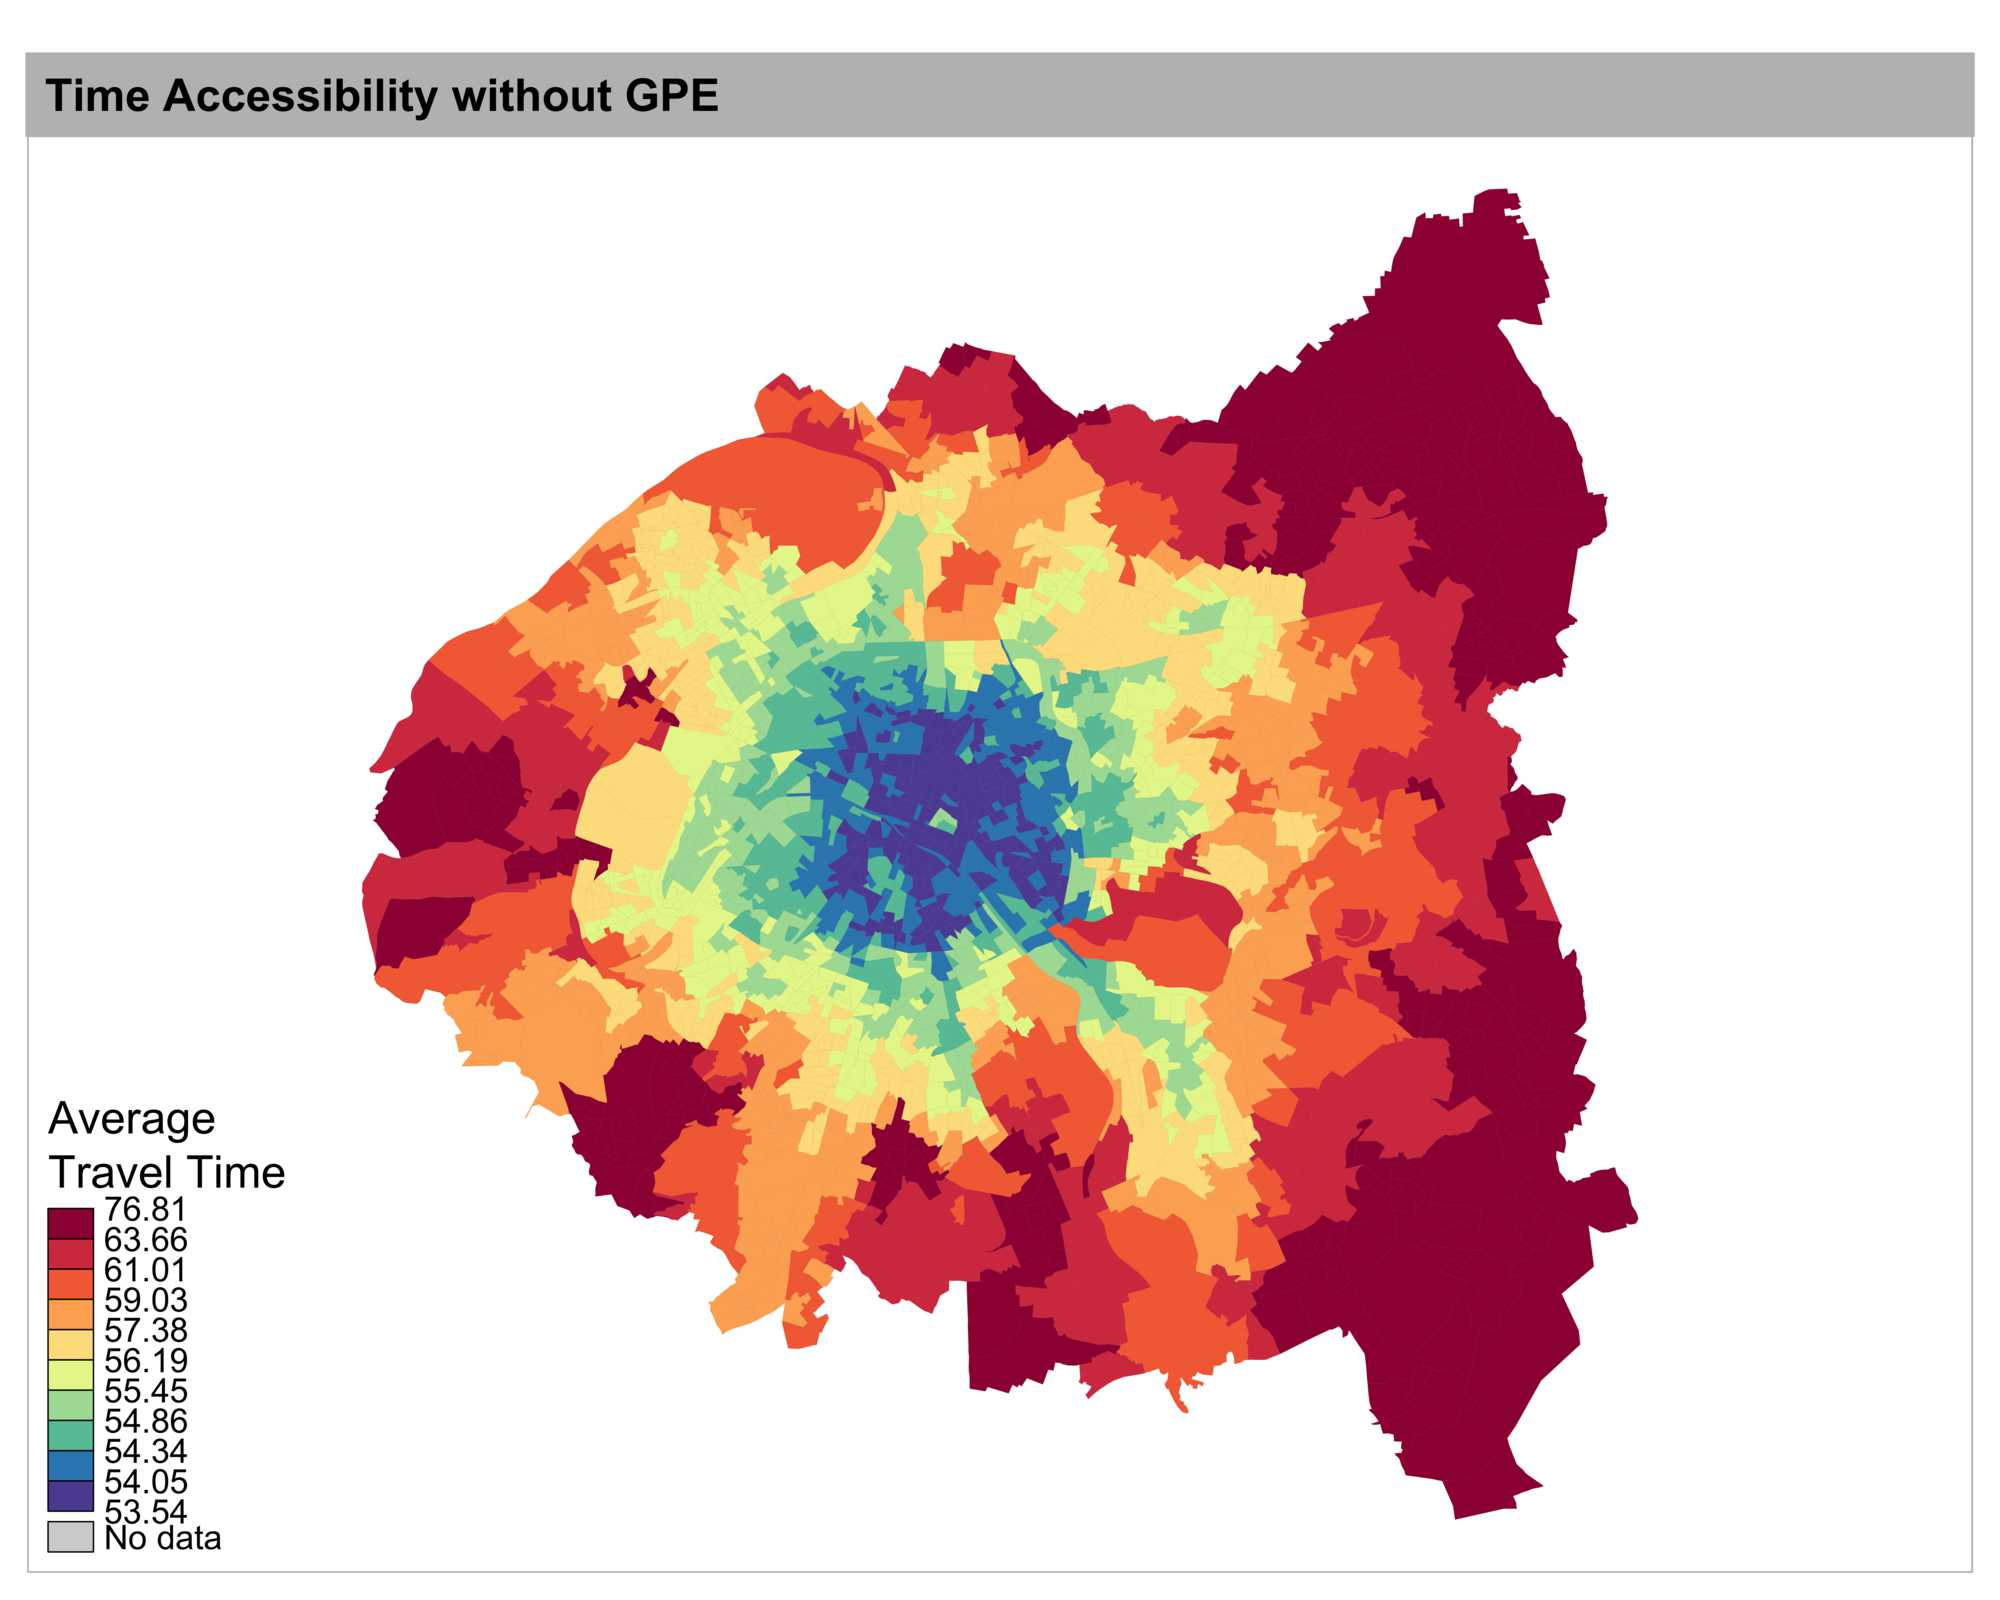
\includegraphics[width=0.8\linewidth]{Figures/CaseStudies/timeaccess_metropole}\\
	%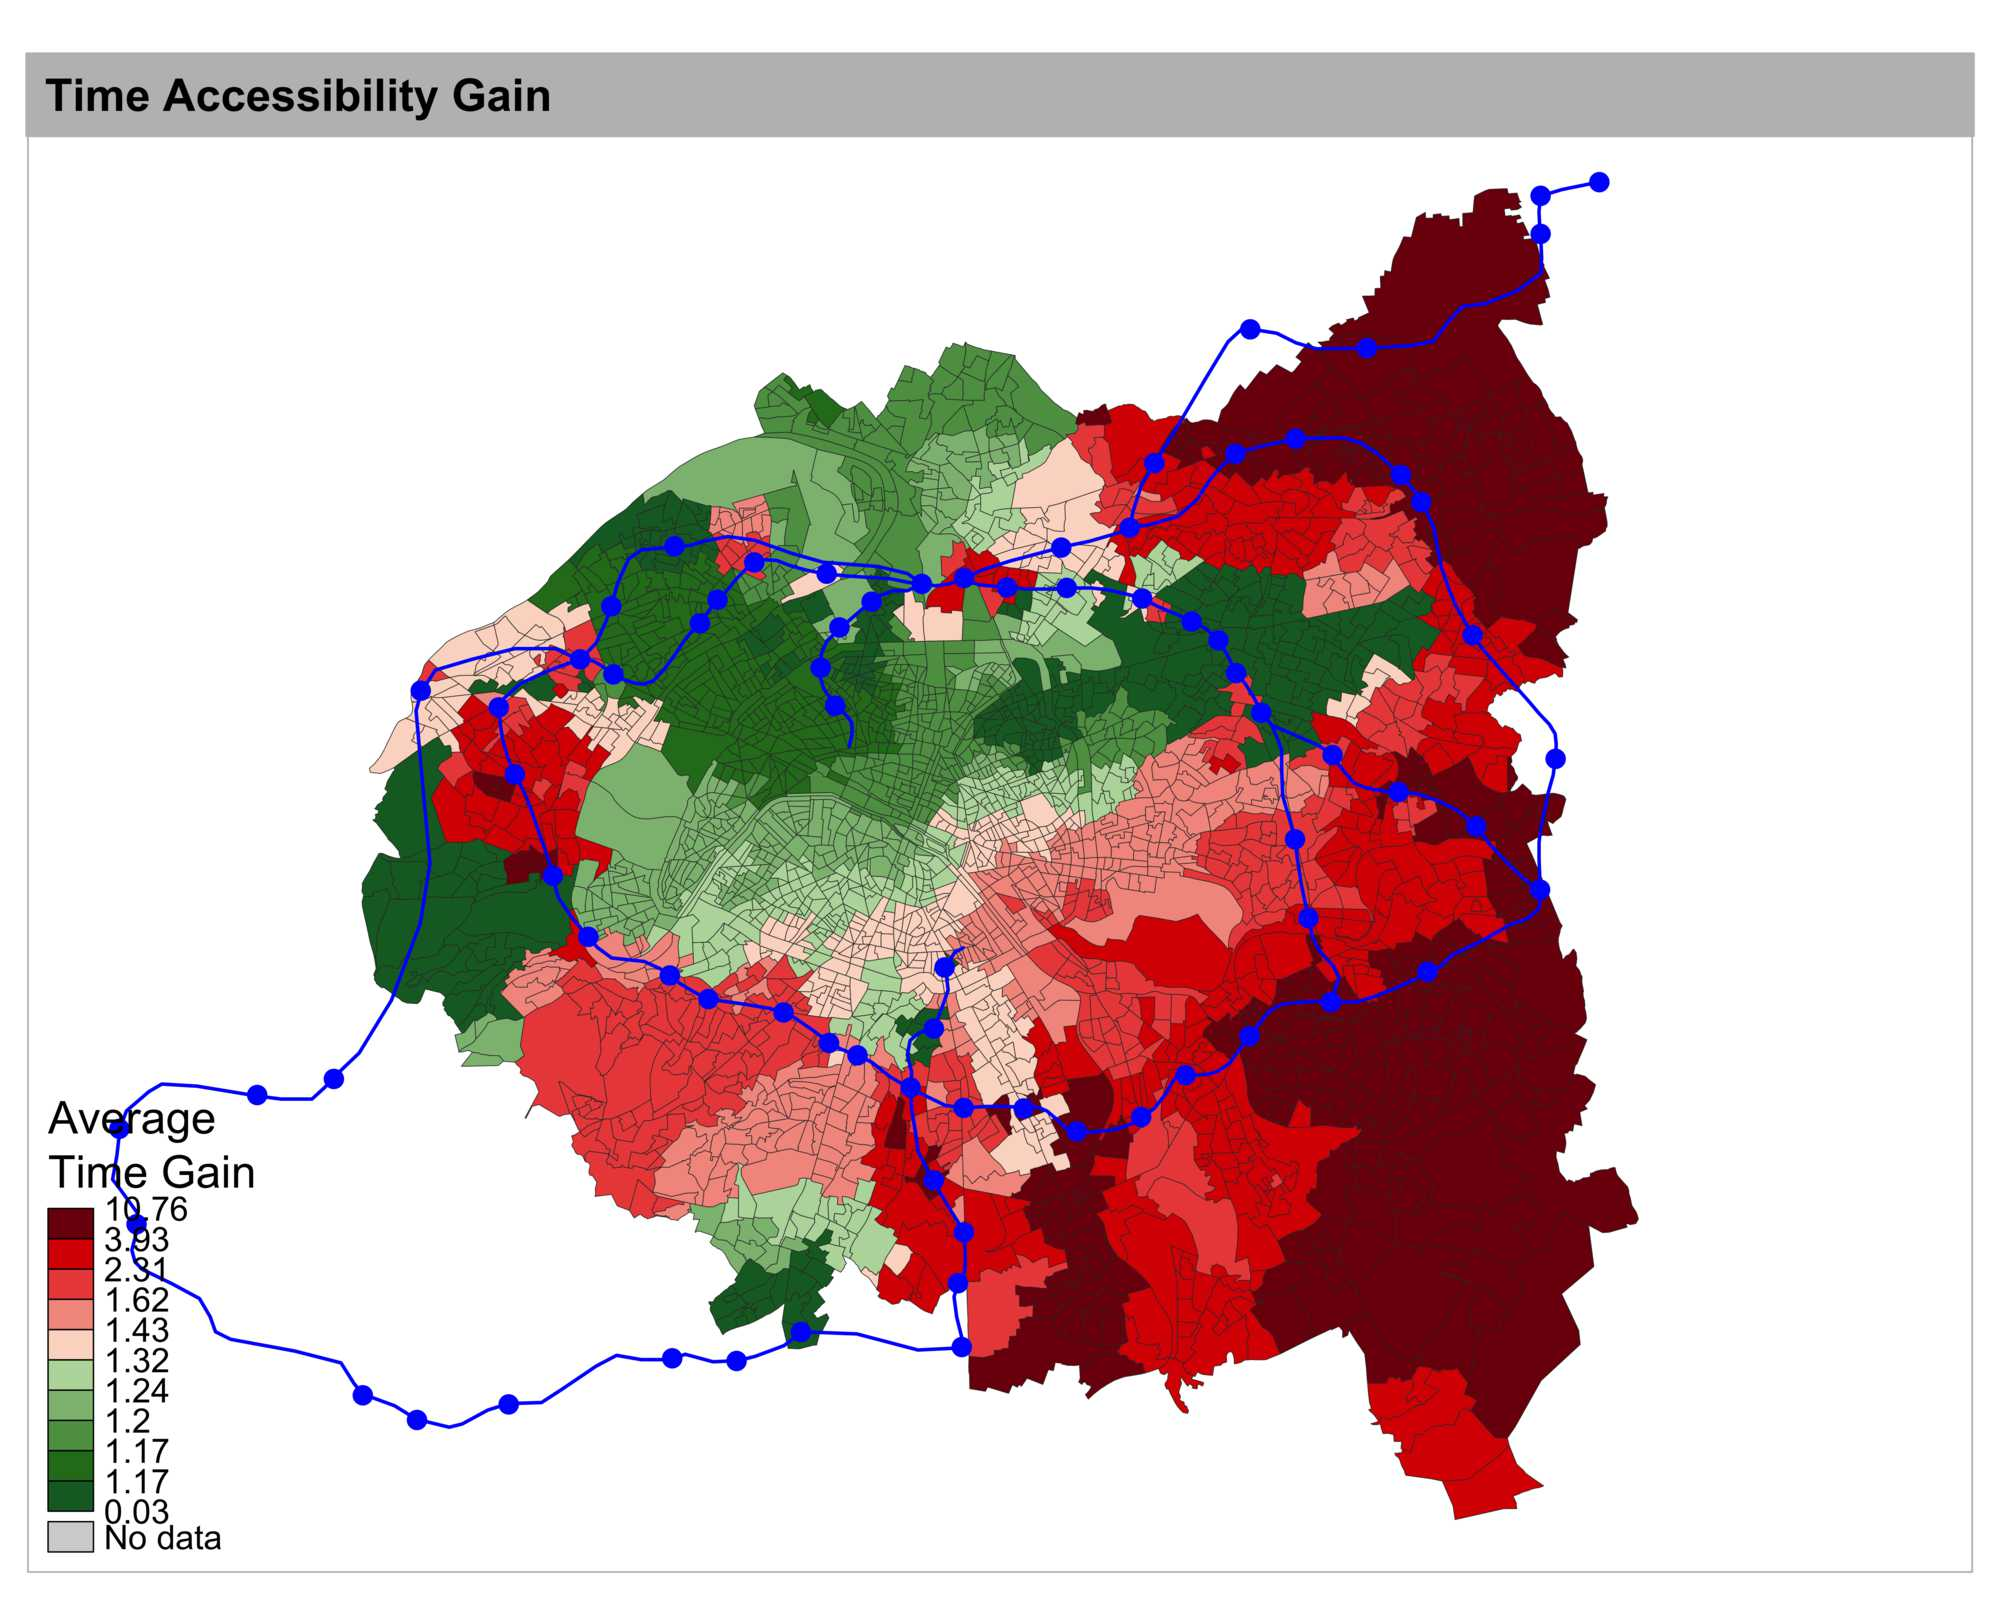
\includegraphics[width=0.8\linewidth]{Figures/CaseStudies/timegain_metropole}
	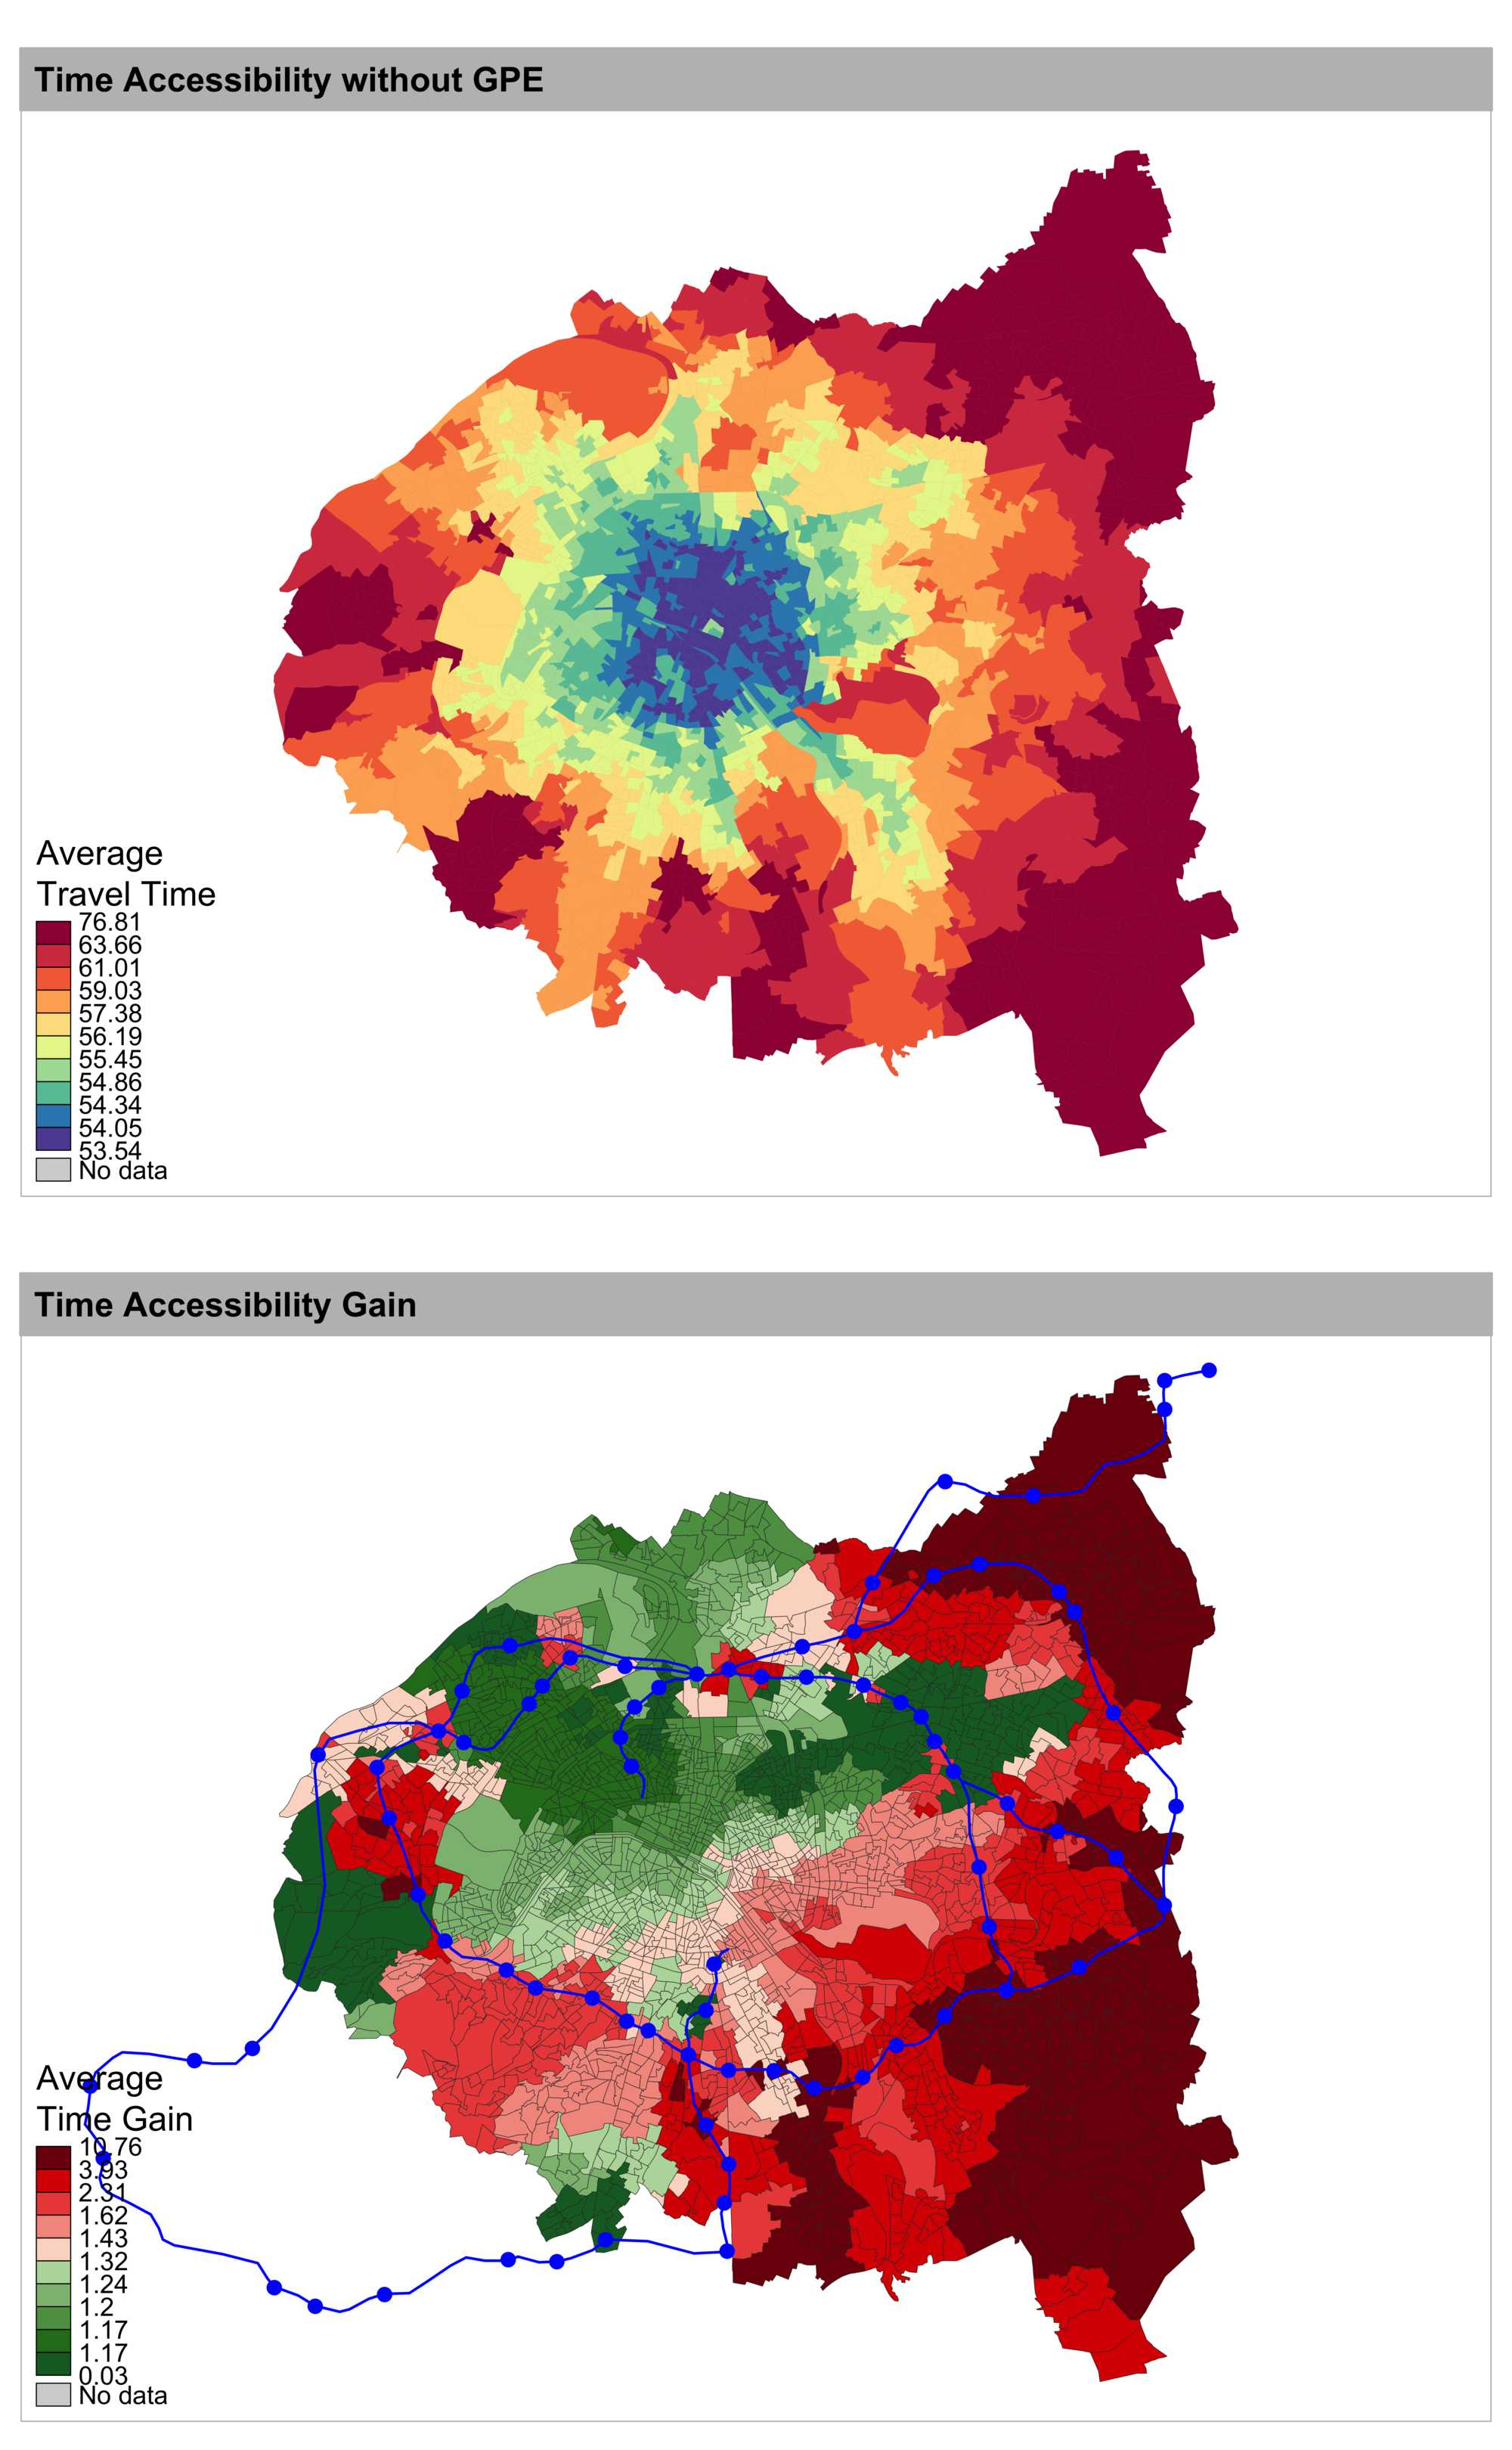
\includegraphics[width=\linewidth]{Figures/Final/1-2-1-fig-casestudies-gpe.jpg}
	\caption[Impact of \emph{Grand Paris Express}][Impact du Grand Paris Express]{\label{fig:casestudies:gpe}}{\textbf{Impact des lignes du GPE sur l'accessibilité temporelle.} \textit{(Haut)} Temps moyen de trajet vers l'ensemble des communes d'Ile-de-France, par transports en commun uniquement, pour les départements métropolitains ; \textit{(Bas)} Gains de temps permis par l'ensemble des lignes du GPE, avec le trajet des lignes.\label{fig:casestudies:gpe}\comment[AB]{traduire ; echelle monotone $\rightarrow$ gradient sur une gamme de couleurs}\comment[FL]{average time gain : entre quoi et quoi ? - gradation de couleurs discutable - pourquoi ces couleurs ? - sens ? ce n'est pas clair du tout - traduire ? que sont les zones ? par ailleurs tu n'as pas les contours de la metropole du grand paris - depuis Iris - communes.}}
\end{figure}
%%%%%%%%%%%%%%%%%%%




\bpar{
Various aspects of territories are concerned by interactions with networks. In previous empirical studies, no socio-economic attributes of populations inhabiting the territory nor economic values for land and real estate was considered. Both are however crucial elements of territorial dynamics and are extensively studied in fields such as territorial analysis or urban economics : for example, \cite{homocianu:tel-00359302} studies households residential choices to understand land-use transportation interactions. We propose here to use a database of Real Estate transactions for Parisian region on the last 20 years, with 2 years temporal granularity and exact spatial coordinates. \cite{guerois2009dynamique} used it to make typologies of spatial dynamics of Parisian real estate.
}{
Des aspects très variés des territoires sont concernés par l'interaction avec les réseaux. Dans nos études précédentes, les aspects économiques et financiers du foncier et l'immobilier n'ont pas été considérés. Il s'agit cependant d'éléments cruciaux des dynamiques territoriales et sont étudiés de manière intensive dans des champs comme l'analyse territoriale ou l'économie urbaine : par exemple, \cite{homocianu:tel-00359302} étudie les choix résidentiels des ménages pour comprendre les interactions entre usage du sol et transport. Nous proposons ici d'utiliser entre autres une base de données de transactions immobilières pour la région parisienne sur les 20 dernières années, avec une granularité temporelle de 2 ans et coordonnées spatiales exactes. \cite{guerois2009dynamique} l'utilise par exemple pour établir une typologie des dynamiques spatiales du marché immobilier parisien.
}


\bpar{
We propose to study the relations between accessibility differentials for each project, with variables linked to real estate and socio-economic variables. Indeed, the links between new lines and real estate value evolution are sometimes dramatic~\cite{damm1980response}. 
}
{
Cette étude plus précise peut être comprise comme une recherche de signes précurseurs de rupture de potentiels du réseau: en effet, si des dynamiques territoriales intrinsèques anticipent l'arrivée d'une nouvelle station de transports en commun, les implications seront bien différentes du cas où celle-ci conduit ces variables après sa construction. L'interprétation en termes ``d'effets structurants'' sera notamment très différente. Nous appliquons ici la méthode de causalités spatio-temporelles développée en~\ref{sec:causalityregimes}. Nous proposons d'étudier les relations entre différentiel d'accessibilité pour chaque projet, et variables liées au foncier (transactions immobilières) et socio-économiques. En effet, les liens entre nouvelles lignes et évolution du foncier sont parfois remarquables~\cite{damm1980response}.
}

\comment{sur les anticipations des acteurs : \cite{carrouet:hal-00980002} }


\cite{guerois2009dynamique} : bulles immobilières locales ?


\bpar{
Data for real estate transactions are contained within the BIENS database (\emph{Chambre des Notaires d'Ile de France}, proprietary database). The number of transactions that can be used after cleaning is 862360, distributed across all IRIS areas (basic census units in France), for a temporal span covering the years 2003 to 2012 included. The data at the IRIS level for population and income (median income and Gini index) come from INSEE. Network data have been vectorialized from projects maps (see figure~\ref{fig:projects} for the different projects). Travel times are computed by public transportation only, with standard values for average speeds of different modes (RER 60km.h\textsuperscript{-1}, Transilien 100km.h\textsuperscript{-1}, Metro 30km.h\textsuperscript{-1}, Tramway 20km.h\textsuperscript{-1}). The travel time matrix is computed from all the centroids of IRIS to all the centroids of \emph{Communes} (above aggregation level). These are linked to the network with abstract connectors to the closest station, with a speed of 50km.h\textsuperscript{-1} (travel by car). Analysis are implemented in R~\cite{rcoreteam} and all data, source code and results are available on an open git repository\footnote{At\\\texttt{https://github.com/JusteRaimbault/CityNetwork/tree/master/Models/SpatioTempCausality/GrandParis}. Data for the BIENS database are given only at the aggregated level of IRIS and for price and mortgage variables, for contractual reasons closing the database.}.
}{
Les données des transactions immobilières sont fournies par la base BIENS (Chambre des Notaires d'Ile de France, base propriétaire). Le nombre de transactions utilisables après nettoyage est de 862360, se répartissant sur l'ensemble des IRIS, pour une plage temporelle couvrant de 2003 à 2012 incluses. Les données par IRIS pour population et revenu (revenu médian et indice de Gini) proviennent de l'INSEE. Les données de réseau ont été vectorialisées à partir des cartes des projets (voir Fig.~\ref{fig:projects} pour les projets). Les temps de trajets sont calculés par transport en commun uniquement, avec des valeurs standard pour les vitesses moyennes des différents modes (RER 60km.h\textsuperscript{-1}, Transilien 100km.h\textsuperscript{-1}, Metro 30km.h\textsuperscript{-1}, Tramway 20km.h\textsuperscript{-1}). La matrice des temps est calculée depuis l'ensemble des centroïdes des IRIS vers l'ensemble des centroïdes des communes. Ceux-ci sont reliés au réseau par des connecteurs à la gare la plus proche, de vitesse 50km.h\textsuperscript{-1} (trajet en voiture). Les analyses sont implémentées intégralement en langage R~\cite{rcoreteam} et l'ensemble des données, du code source et des résulats sont disponibles sur un dépôt git ouvert\footnote{A l'adresse\\\texttt{https://github.com/JusteRaimbault/CityNetwork/tree/master/Models/SpatioTempCausality/GrandParis}. Les données de la base BIENS ne sont fournies que de manière agrégée à l'IRIS et pour les variables de prix et de crédit, pour des raisons de fermeture contractuelle de la base brute.}.
}



%%%%%%%%%%%%%%%
\begin{figure}
%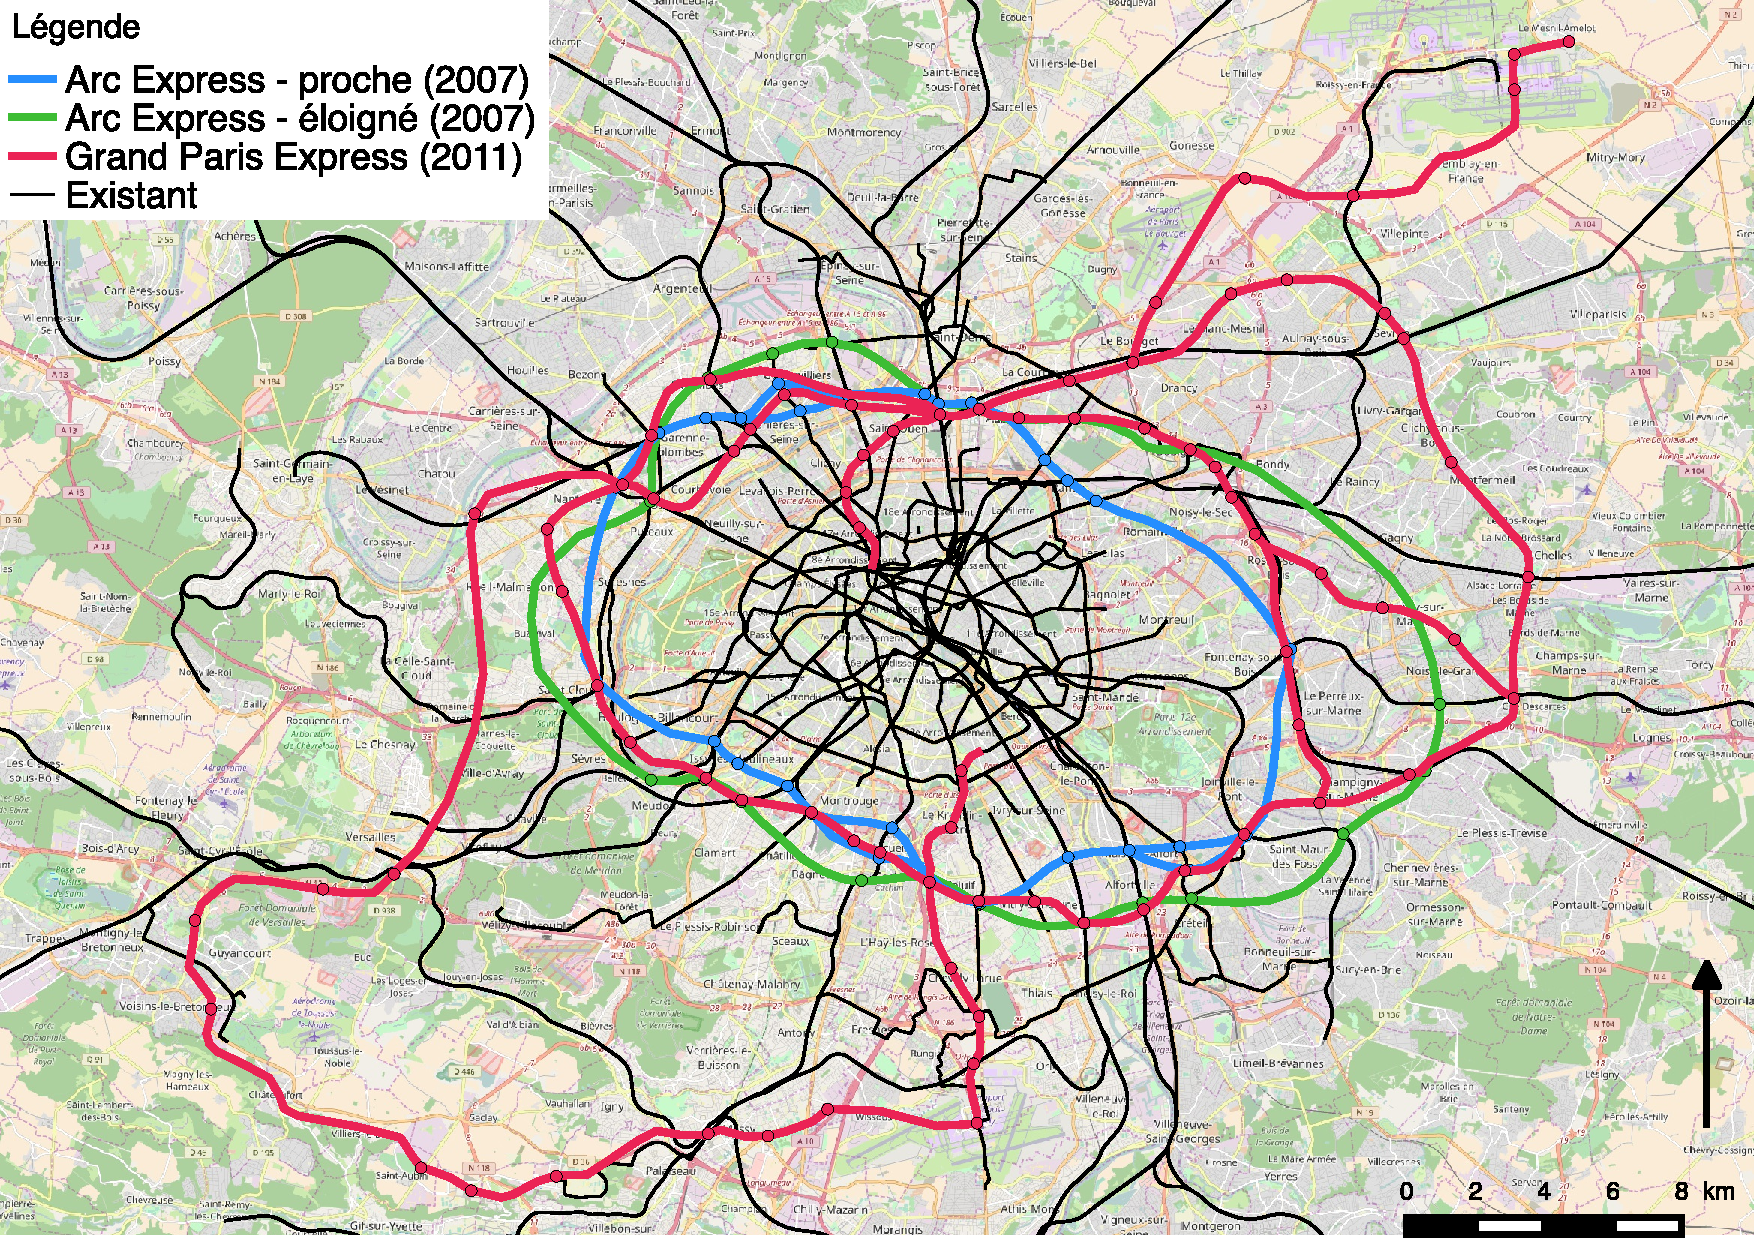
\includegraphics[width=\linewidth]{Figures/GrandParisRealEstate/reseaux}
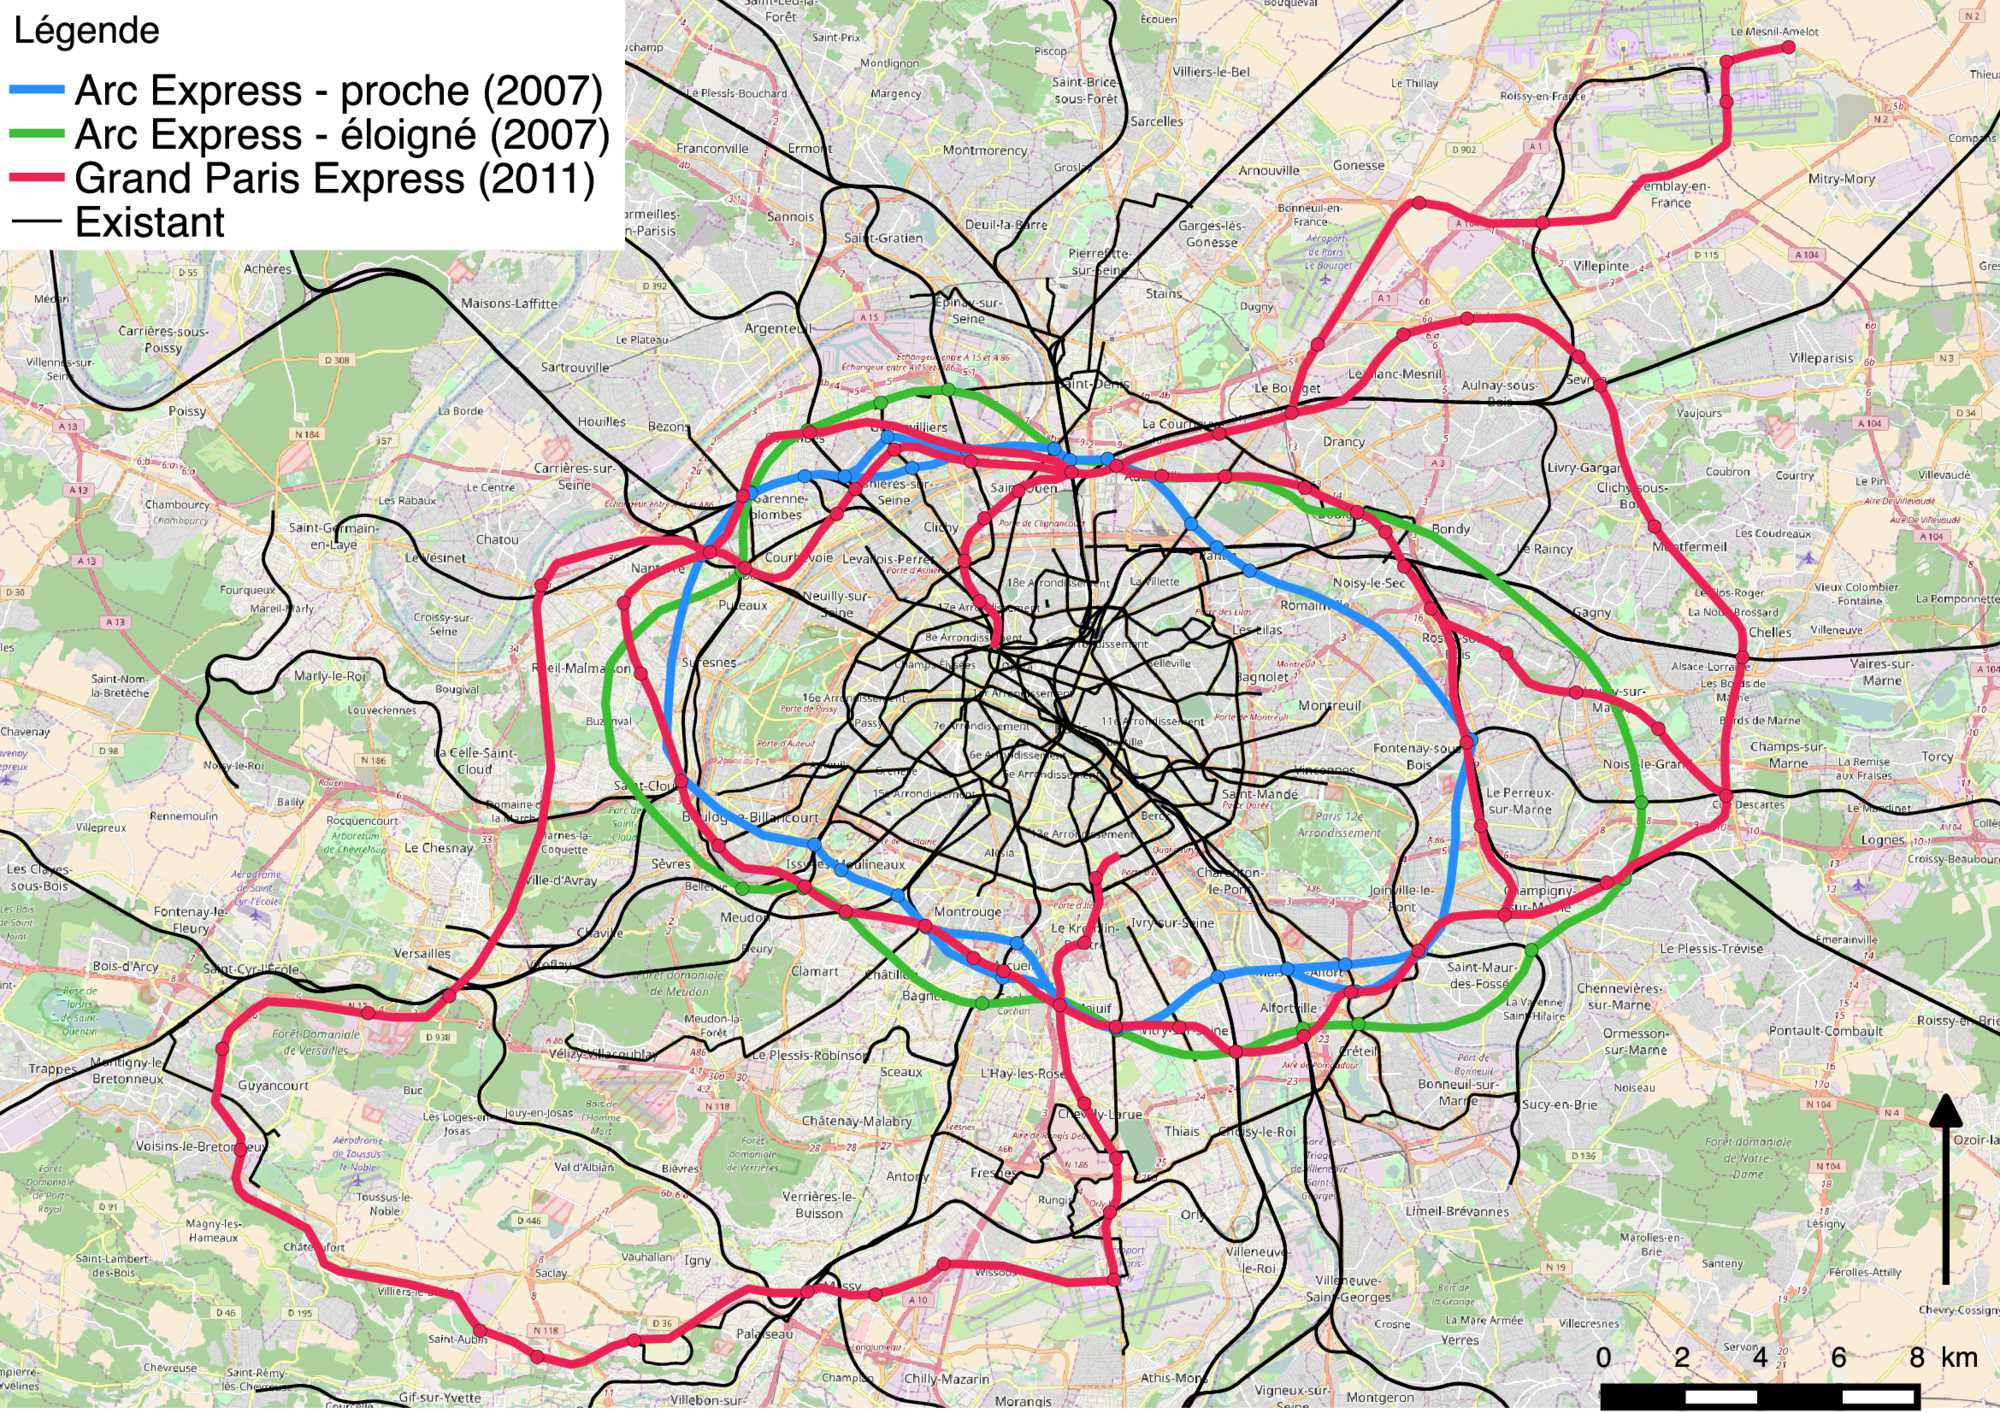
\includegraphics[width=\linewidth]{Figures/Final/1-2-1-fig-casestudies-projects.jpg}
\caption[][Projets de transport successifs du Grand Paris]{\textbf{Successive transportation network projects for the Grand Paris metropolitan area.} We show the two alternatives for the \emph{Arc Express} project elaborated by the Region, and the \emph{Grand Paris Express} (GPE) advocated by the State. The \emph{Réseau du Grand Paris}, a precursor for GPE, is not shown here for visibility reasons because of its proximity with it.\label{fig:projects}}{\textbf{Projets de transport successifs de la métropole du Grand Paris.} Nous montrons les deux alternatives du projet Arc Express porté par la région, et le Grand Paris Express (GPE) porté par l'état. Le Réseau du Grand Paris, précurseur du GPE, n'est pas montré ici pour des raisons de visibilité à cause de sa proximité avec celui-ci.\label{fig:casestudies:projects}}
\end{figure}
%%%%%%%%%%%%%%%


\bpar{

We compute for each project accessibility differentials $\Delta T_i$ in average travel time from each IRIS, in comparison with the network without the project. Average travel time accessibility is defined as $T_i = \sum_k \exp{-t_{ik}/t_0}$ with $k$ \emph{Communes}, $t_{ik}$ travek time, and $t_0$ a decay parameter. To each project is associated a date\footnote{2006 for \emph{Arc Express}, 2008 for \emph{Réseau du Grand Paris} and 2010 for \emph{Grand Paris Express}}, corresponding roughly to the mature announcement of the project. It stays a bit arbitrary as it is difficult on the one hand to determine precisely as a planning project does not emerge from nothing in one day, and one the other hand it may correspond to different realities of learning about the project by economic agents (we do therefore the limiting but necessary assumption of a diffusion of information for the majority of agents in a time smaller than a year). We study the lagged correlations of this variable with the variations $\Delta Y_{ij}$ of the following socio-economic variables: population, median income, Gini index for income, average price of real estate transactions and average value of real estate mortgages. A Fisher test is done for each estimation and the value is set to 0 if it is not significant ($p<0.05$ in a classical manner). The study with generalized accessibility in the sense of Hansen has also been conducted but is less interesting as it has a very low sensitivity to the mobility component (network and decay) compared to the variables themselves. It informs therefore only on relations between these and is not presented here.
}{
Nous calculons pour chaque projet, le différentiel $\Delta T_i$ d'accessibilité en temps moyen de trajet à partir de chaque IRIS en comparaison à celui dans le réseau sans le projet, défini par $T_i = \sum_k \exp{-t_{ik}/t_0}$ avec $k$ communes, $t_{ik}$ temps de trajet, et $t_0$ paramètre d'atténuation. A chaque projet est associée une date\footnote{2006 pour Arc Express, 2008 pour le Réseau du Grand Paris, 2010 pour le Grand Paris Express}, correspondant environ à l'année d'annonce mature du projet, restant toutefois arbitraire car difficile d'une part à déterminer précisément, un projet n'émergeant pas d'un coup du jour au lendemain, et d'autre part pouvant correspondre à des réalités différentes d'apprentissage du projet par les différents agents économiques (nous faisons donc l'hypothèse réductrice mais nécessaire d'une diffusion sur la majorité des agents dans un temps inférieur à l'année). Nous étudions les corrélations décalées de cette variable avec les variations $\Delta Y_{ij}$ des variables socio-économiques suivantes : population, revenu médian, indice de Gini des revenus, prix moyen des transactions immobilières et montant moyen des crédits immobiliers. Un test de Fisher est effectué pour chaque estimation, et la valeur est fixée nulle si celui-ci n'est pas significatif ($p<0.05$ de manière classique). L'étude avec accessibilité généralisées au sens de Hansen a également été menée mais moins intéressante car très peu sensible à la composante mobilité (réseau et atténuation) par rapport aux variables elle-même, informe uniquement sur des relations entre celles-ci et n'est donc pas présentée ici.
}


\bpar{
We show in figure~\ref{fig:empiricalres} the results for all networks and variables. It is first remarkable to note the presence of significant effects for all variables. Lower values for the parameter $t_0$ give correlations higher in absolute value, unveiling a possible higher importance of local accessibility on territorial dynamics. The behavior of population shows a clearly detached peak corresponding to 2008, what suggests an impact of the older project \emph{Arc Express} on population growth, the effect of other projects would then be spurious from their proximity in the most important branches. It would imply that areas where they are fundamentally different such as \emph{Plateau de Saclay} are less sensitive to transportation projects, what would confirm the artificial planned aspect of the development of this territory. Concerning income, we observe a similar behavior but in a negative way, what would imply a decrease of wealth linked to the increase of accessibility, however accompanied by a decrease of inequalities. Finally, real estate prices are as expected driven by the potential arrival of new networks. This effect disappear after two years for the \emph{Grand Paris Express}, suggesting a temporal speculation bubble. We demonstrate thus the existence of complex lagged correlation links, that we call causalities in this sense, between territorial dynamics and anticipated dynamics of networks. A finer understanding of working processes is beyond the scope of this paper and would imply for example qualitative fieldwork or targeted case studies. This example shows however the operational potentialities of our method on a real case study.

}{
Nous présentons en Fig.~\ref{fig:empiricalres} les résultats pour l'ensemble des réseaux et variables. Il est remarquable tout d'abord de noter l'existence d'effets significatifs pour l'ensemble des variables. Des valeurs plus basses du paramètre $t_0$ donnent des corrélations plus fortes en valeur absolue, révélant une possible plus grande importance de l'accessibilité locale sur les dynamiques territoriales. Le comportement de la population montre un pic très détaché correspondant à 2008, laissant supposer un impact du plus vieux projet d'Arc Express sur la croissance de la population, l'effet des autres projets serait alors fallacieux de par leur proximité dans les grands tronçons : cela impliquerait que les zones où ils diffèrent fondamentalement comme le Plateau de Saclay ne soient que très peu sensibles au projet de transport, ce qui confirmerait l'aspect artificiel planifié du développement de ce territoire. Concernant les revenus, on observe un comportement similaire mais négatif, ce qui impliquerait un appauvrissement lié à l'augmentation de l'accessibilité, mais qui semble toutefois s'accompagner d'une baisse des inégalités. Enfin, comme attendu les prix immobiliers sont tirés par l'arrivée potentielle des nouveaux réseaux, effet qui disparait à deux ans pour le Grand Paris Express, suggérant une bulle immobilière passagère. Nous démontrons ainsi l'existence de liens de correlations retardées complexes qu'on nomme causalités en ce sens, entre dynamiques territoriales et dynamiques anticipées des réseaux. Une compréhension plus fine des processus à l'oeuvre est au delà de la portée de cet article, car supposerait des études de terrain qualitatives, des études de cas ciblées, etc. Cet exemple illustre cependant le caractère opérationnel de notre méthode sur un cas d'étude réel.
}




%%%%%%%%%%%%%%%
\begin{figure}[h!]
%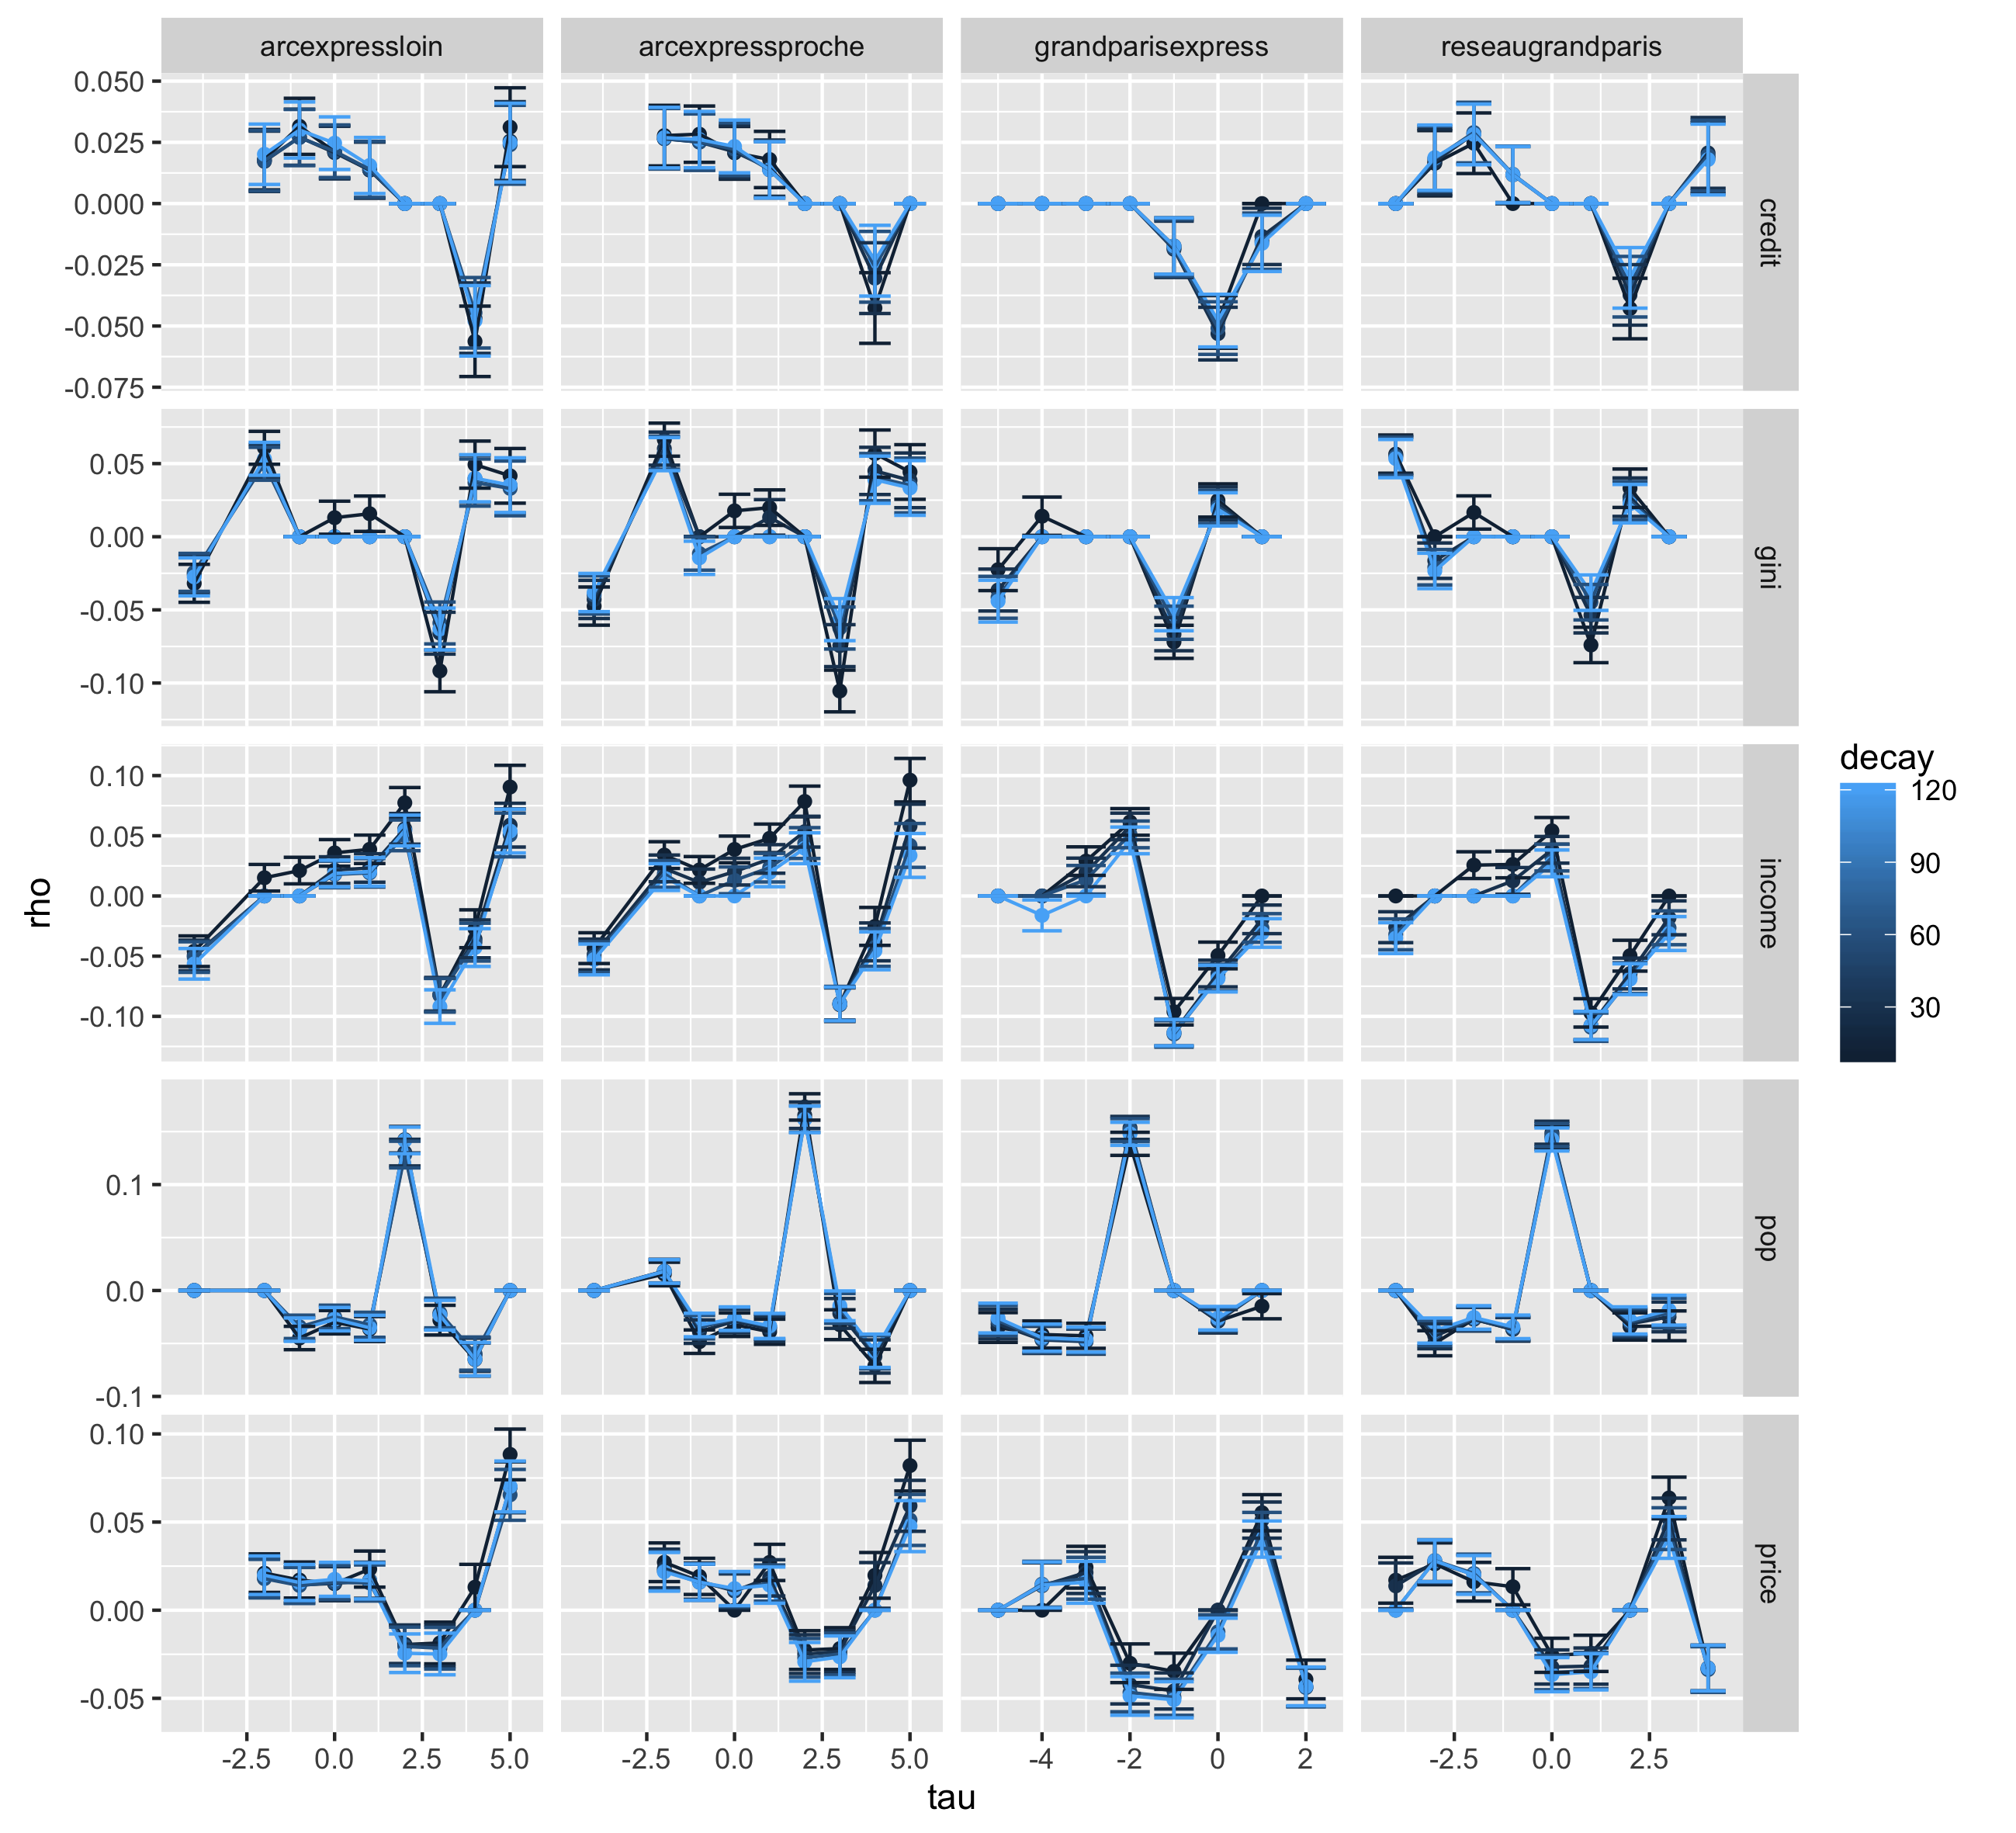
\includegraphics[width=\linewidth]{Figures/GrandParisRealEstate/laggedcorrs_times_allvars}
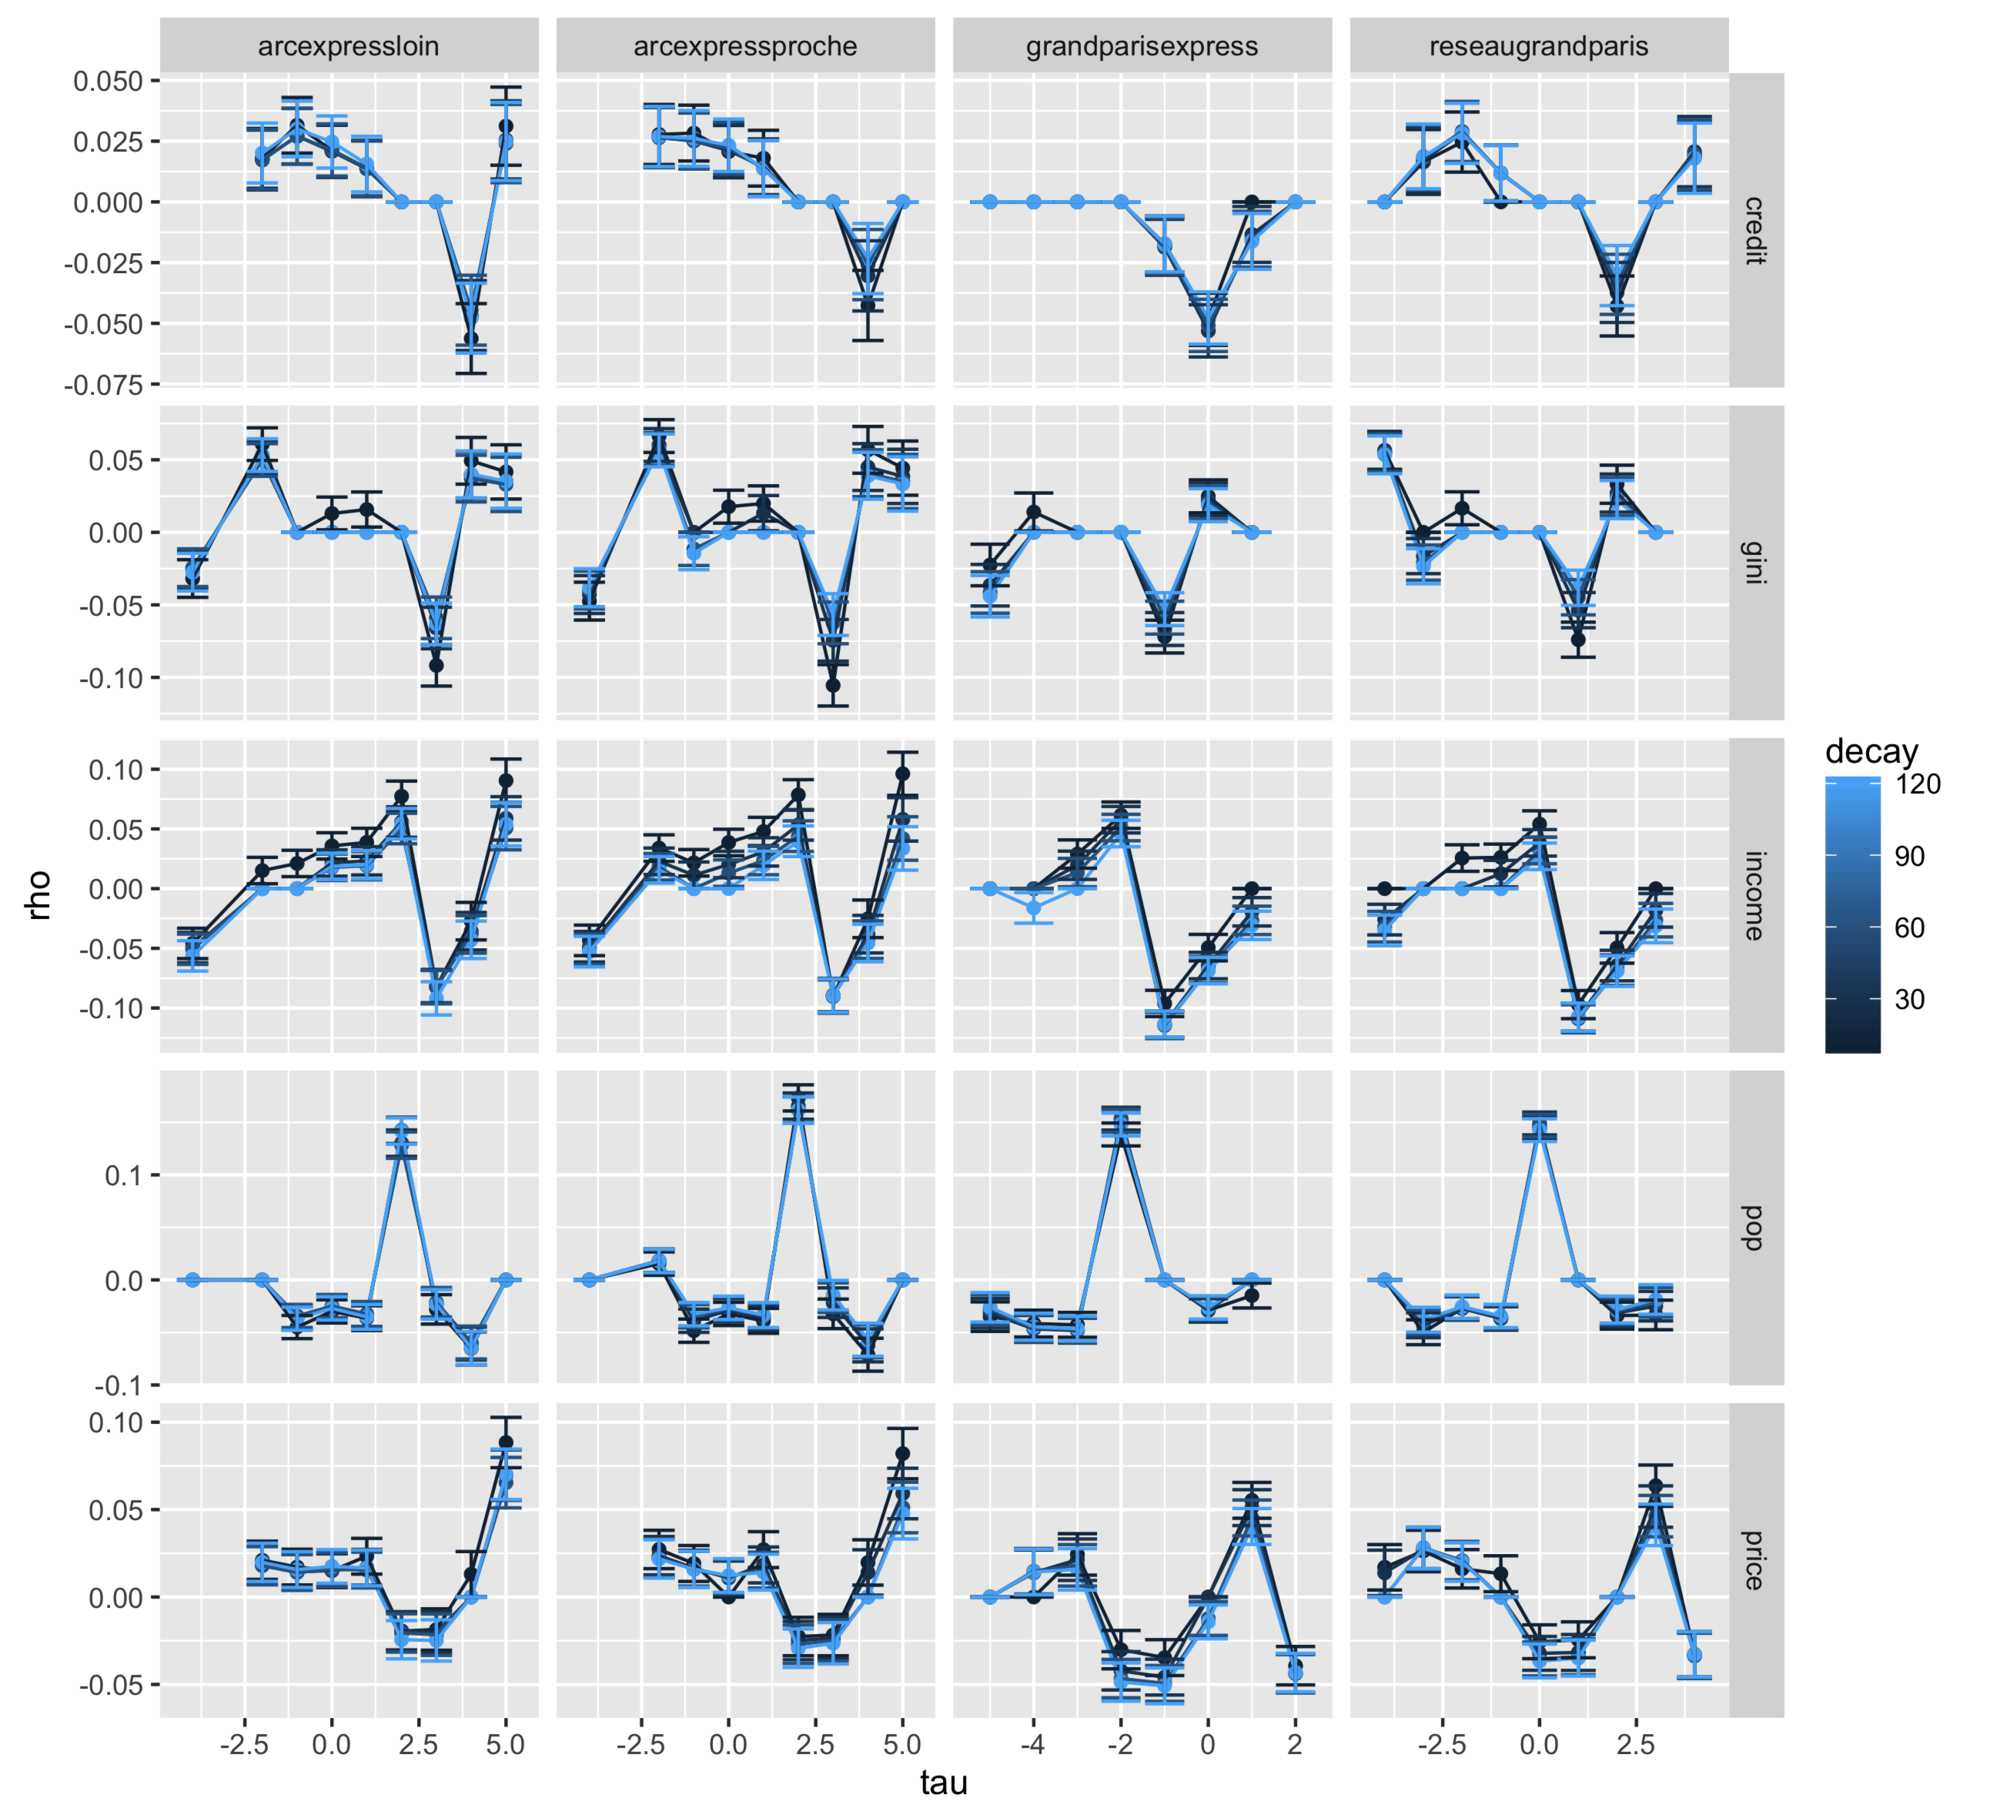
\includegraphics[width=\linewidth]{Figures/Final/1-2-1-fig-casestudies-empiricalres.jpg}
\caption[][Corrélations retardées empiriques]{\textbf{Empirical lagged correlations.} Plots show the value of lagged correlation between accessibility differentials in average travel time $\Delta T$ for each project (in colunms) and socio-economic and real estate variables variations (in rows). All are computed for different values of the decay parameter (\texttt{decay}, given by curve color). Error bars give the 95\% confidence interval.\label{fig:empiricalres}}{\textbf{Corrélations retardées empiriques.} Les graphiques donnent la valeur de la correlation entre le différentiel d'accessibilité en temps de trajet moyen $\Delta T$ pour chaque projet (en colonnes) et le différentiel des différentes variables socio-economiques et de transactions immobilières (en lignes), pour différentes valeurs du paramètre d'atténuation (\texttt{decay}). Les barres d'erreur donnent l'intervalle de confiance à 95\%.\label{fig:casestudies:empiricalres}}
\end{figure}
%%%%%%%%%%%%%%%
















%-------------------------


%%%%%%%%%%%%%%%%%%%%%%%%
%\subsection[Pearl River Delta][Le Delta de la Rivière des Perles]{Pearl River Delta: new urban regimes and mega-city regions}{Le Delta de la Rivière des Perles : nouveaux régimes urbains et Mega-région urbaine}
\subsection{Pearl River Delta}{Le Delta de la Rivière des Perles}


\paragraph{New urban regimes and mega-city regions}{Nouveaux \emph{régimes urbains} et \emph{Mega-région urbaine}}

\bpar{}{
Si la notion de megalopolis peut être tracée jusqu'à \noun{Gottmann}~\cite{gottmann1964megalopolis}, et qu'elle est à l'origine de celle de \emph{Mega-city Region} (MCR) consacrée par \noun{Hall}~\cite{hall2006polycentric},\comment[FL]{cest tres tres rapide, a reprendre} il est clair que cette dernière est toujours plus d'actualité avec l'apparition récente de nouveaux régimes, notamment par l'urbanisation accélérée dans des pays à forte croissance économique et en mutation très rapide comme la Chine~\cite{swerts2015megacities}. Le second cas que nous développons ici rentre dans cette catégorie : le Delta de la Rivière des Perles (PRD) est une des illustrations classiques de la structure d'une MCR fortement polycentrique. Historiquement initialement composé de Guangzhou uniquement, le développement de Hong-Kong puis la mise en place des Zones Economiques Spéciales dans le cadre des politiques d'ouverture de \noun{Deng Xioaping}, a conduit à un développement extrêmement rapide de Shenzhen, et dans une moindre mesure de Zhuhai. La province du Guangdong dans lequel le PRD se situe intégralement a actuellement le plus fort PIB régional de Chine, et la MCR regroupe une population d'environ 60 millions (les estimations fluctuant fortement selon la définition prise de la MCR et la prise en compte de la population flottante). Le phénomène de migration des campagnes est très présent dans la région et une ville comme Dongguan a par exemple basé son économie sur des manufactures employant ces travailleurs migrants.
}


\bpar{}{
\cite{Ye2014200} analyse les actions de gouvernance métropolitaine à l'échelle de centres de la MCR, et plus particulièrement comment les communes de Guangzhou et Foshan ont progressivement accru leur coopération pour former une zone métropolitaine intégrée, pouvant ainsi fortement influencer le développement des transports par exemple et permettant la mise en place d'un réseau connecté. Une forte tension entre des processus émergents par le bas, et un dirigisme d'état relativement fort en Chine, se répercutant de l'Etat central, au gouvernement provincial jusqu'aux gouvernements locaux, a permis la mise en place d'une telle structure. La compétition avec les autres villes de la MCR reste très forte, et la logique d'intégration\comment[FL]{explicite ce que cela peut signifier} de la MCR est partiellement guidée par la région seulement. La nature particulière des ZES de Shenzhen et Zhuhai, liée aux relations privilégiées avec les Zones Administratives Spéciales de Hong-Kong et Macao, qui n'ont été réintégrées à la République Populaire qu'à la fin du millénaire et conservent un certain niveau d'indépendance en termes de gouvernance, complique encore les jeux d'acteurs au sein de la région. La question d'un niveau de gouvernance qui expliquerait tel ou tel processus urbain est épineuse\comment[FL]{pourquoi vouloir priviliegier 1 niveau de gouvernance ?} : \cite{liao2017ouverture} interprète les transferts progressifs des initiatives économiques du pouvoir central vers les autorités locales comme une forme de gouvernance multi-niveaux. Dans le cadre des transports pour la MCR, il n'existe pas d'autorité d'organisation des transports, et chaque commune gère indépendamment le réseau local, tandis que les connections entre villes sont assurées par le réseau de train national. Cela conduit à des situations particulières dans lesquelles des zones se retrouveront très enclavées, avec une hétérogénéité très forte localement. Ainsi, la pointe sud de la ville de Guangzhou qui sert d'accès direct à la mer, est plus proche géographiquement du centre de Zhongshan, mais un lien direct par transports en commun est difficile à envisager, alors que la zone est bien reliée au centre de Guangzhou par la ligne de métro. Une situation similaire s'observe au terminus de la ligne 11 de Shenzhen, pour le quartier limitrophe de Dongguan, ce dernier étant très peu accessible. Cette situation serait cependant transitoire, étant donné les infrastructures déjà en construction et celles planifiées sur un plus long terme : le métro de Shenzhen, qui couvre aujourd'hui 285km, est planifié jusqu'à 30 lignes et 1142km\comment[FL]{c'est absolument considerable le dire (et verifier que c'est vrai)}[// IDF voies rapides ; ordres de grandeur] en 2030~\cite{shenzhen2016plan}. Il est clair que ces développements suivent pour la majorité un développement urbain existant, une question cruciale est la volonté et la capacité à contenir l'étalement urbain et structurer les futurs développements autour de ce nouveau réseau, dans l'esprit d'une intégration volontaire entre urbanisme et transport de type Transit Oriented Development.\comment[FL]{que tu n'as pas defini} Différents terminus seront connectés au metro de Dongguan, et de nouvelles lignes intercités structureront les déplacements de plus longue portée, ce qui fera du Delta dans un horizon temporel proche une MCR relativement bien intégrée en termes de transports en communs.
}


\paragraph{Impact of the Zhuhai-Hong-Kong-Macao bridge}{Impact du Pont Zhuhai-Hong-Kong-Macao}

Un projet iconique d'infrastructure de transport dans la région est le pont-tunnel fermant l'embouchure du Delta, reliant Zhuhai et Macao à Hong-Kong.\comment[FL]{faire une carte} La longueur de la traversée est de 36.5km, ce qui en fait un ouvrage d'art exceptionnel. L'ouverture au traffic a été retardée de plusieurs années et est prévue finalement pour fin 2017\footnote{voir \texttt{http://www.hzmb.org/cn/default.asp}}. \cite{zhou2016medium} montre que les changements de motifs d'accessibilité attendus pour l'Ouest du Delta sont relativement forts, et ceux-ci peuvent potentiellement induire de fortes bifurcations dans les trajectoires des villes. La nécessité du projet est supportée par une narration\comment[FL]{que veux tu dire ?} de fort bénéfice économique dans le cadre des politiques d'ouverture, ainsi que par un bénéfice social pour l'Ouest notamment. Par exemple, Zhuhai se positionne comme un nouveau pivot entre Hong-Kong et l'ouest. L'équilibrage d'accessibilité\comment[FL]{sens ?} s'opère cependant pour le mode routier uniquement, ce qui conduit à questionner ses impacts potentiels : d'une part l'accès à l'automobile reste réservé à une partie de la population seulement, d'autre part les externalités négatives\comment[FL]{?} de congestion peuvent rapidement modérer les gains d'accessibilité. Les impacts à moyen et long terme du pont sont ainsi difficiles à estimer, une piste étant de poser le problème différemment et de chercher comprendre la dynamique du système métropolitain de manière intégrée\comment[FL]{c'est tres elliptique}, comme nous l'évoquerons en~\ref{sec:lutetia}.





%-------------------------


%%%%%%%%%%%%%%%%%%%%%%%%
\subsection{Comparability of case studies}{Comparabilité des études de cas}


La possibilité de transfert des modèles\comment[FL]{def} urbains est délicate, et la particularité Est-asiatique a déjà été montrée pour la structure économique, et comment celle-ci ne peut être interprétée de manière simple par une séparation des processus microscopiques et macroscopiques comme certaines lectures rapides et idéologiquement orientée ont pu le faire, comme la vision de la Banque Mondiale~\cite{amsden1994isn}. La comparabilité de systèmes urbains est une question ouverte au centre des enjeux de la Théorie Evolutive Urbaine, et est par exemple liée au caractère ergodique de ces systèmes : si la trajectoire d'une ville dans le temps capture l'ensemble des états urbains possibles, alors les différentes villes sont différentes manifestations du même processus stochastique à différentes périodes, et un ensemble de villes permettrait de se faire une idée des trajectoires temporelles.\comment[FL]{c'est trop rapide} Intuitivement ce n'est pas le cas, et la Théorie Evolutive postule en effet la non-ergodicité~\cite{pumain2012urban}, que nous étudierons plus en détail en~\ref{sec:staticcorrelations}.







\stars





%
% 1.3 Qualitative Research


%-------------------------

\newpage


\section{Fieldwork elements}{Elements de terrain}

\label{sec:qualitative}


%-------------------------


Cette section propose d'illustrer la problématique des interactions entre réseaux de transports et territoires, et plus particulièrement leur complexité et la diversité des situations possibles déjà perceptibles de manière qualitative (et également subjective dans un second temps) à l'échelle microscopique, par des exemples concrets de terrain. Le terrain géographique est le Delta de la Rivière des Perles en Chine , dans la province du Guangdong, que nous avons décrit ci-dessus, et plus particulièrement en grande partie la ville de Zhuhai. Des observations ont également été effectuées en métropole Parisienne. Nous assumons le terme de \emph{Terrain géographique}, en toute conscience des débats épistémologiques que peuvent poser l'utilisation de celui-ci. En effet, \comment[JR]{court developpement sur epistemo du terrain}

% (\cn{珠江三角洲}) (\cn{广东}) (\cn{珠海})

Dans le cadre du projet européen Medium\footnote{Le project Medium, qui met en partenariat des université européennes et chinoise, s'intitule ``\textit{New pathways for sustainable urban development in China’s medium-sized cities}. Il vise à étudier la soutenabilité selon un prisme interdisciplinaire et multidimensionnel, dans le cas de zones urbaines en forte croissance. Trois villes moyennes chinoise ont été choisies comme cas d'étude. Voir \url{http://mediumcities-china.org/} pour plus d'information.}, visant à une approche interdisciplinaire de la soutenabilité pour les villes Chinoises en se concentrant sur les villes moyennes, cette ville a été choisie comme cas d'étude\comment[FL]{ce n'est pas pertinent ici}. Lorsque la source n'est pas explicitement précisée, les observations proviennent du travail de terrain, pour lequel des compte-rendus narratifs sont disponibles en Annexe~\ref{app:sec:qualitative}. Le format de ceux-ci est ``à-la-volée'' suivant les recommandations de \cite{goffman1989fieldwork} pour la prise de notes en terrain d'immersion notamment, tandis que la position volontairement subjective rejoint \cite{ball1990self} qui souligne l'importance de la réflexivité pour tirer des conclusions rigoureuses à partir d'observations qualitatives de terrain duquel le chercheur est partie intégrante\footnote{La considération du chercheur comme \emph{sujet} en relation avec son objet d'étude n'implique pas dans notre cas de rétroaction du chercheur sur le système vu l'ampleur de celui-ci dans le cas d'un réseau de transport à l'échelle d'une ville, mais bien un conditionnement des observations par une subjectivité dont il s'agit de se détacher dans l'exploitation postérieure du matériau d'observation, mais qu'ignorer ne peut qu'augmenter les biais.}.




%----------------------------



%%%%%%%%%%%%%%%%%%%%%
\subsection{Transportation network development}{Développement d'un réseau de transport}



\bpar{
One main axis of the fieldwork research in China was to get a subjective view of multiple aspects and layers of the complex and ever-changing public transportation system, in Zhuhai as an illustration for local transportation but also at larger scales in China. Indeed, transportation network modeling or data analysis such as accessibility studies or land-use transport interaction models I develop as the main focus of my thesis, generally fail to grasp microscopic aspects that can become crucial when it comes to the effective use of the network. For example, multimodality can be made effective in practice through self-organized informal transportation modes that solve the ``last-mile'' kilometer problem~\cite{liu2012solving} that seems to be often forgotten in the planning of newly developed areas in China. Or in the contrary, practical details such as ticket booking or check-in delays can drastically change use patterns.
}{
L'un des axes principaux de la recherche de terrain en Chine\comment[FL]{tu ne dis pas ce que tu cherches. on ne fait pas de terrain sans raison !} a été de construire une vue subjective des multiples facettes et couches d'un système de transport public complexe et en mutation permanente. La portée des observations s'étend sur Zhuhai comme illustration des transports locaux mais aussi ponctuellement sur d'autres régions en Chine. Ces observations ont une logique propre en comparaison de la modélisation des réseaux de transport ou l'analyse de données, comme des études d'accessibilité ou des modèles d'interaction entre usage du sol et transport, qui seront menés par la suite. En effet, celles-ci échouent généralement à capturer des aspects microscopiques\comment[FL]{def} qui peuvent devenir cruciaux au regard de l'utilisation effective du réseau. Par exemple, la multi-modalité\footnote{La multi-modalité consiste en la combinaison de différents modes de transports : routier, train, métropolitain, tramway, bus, modes doux, etc., dans un motif de mobilité. Un système de transport multimodal consiste en la superposition des couches modales, et celles-ci peuvent plus ou moins bien s'articuler pour la production de trajets optimaux selon de multiples objectifs (coût, temps, coût généralisé, confort, etc.) qui eux-même dépendent de l'individu, du motif de déplacement.} peut être rendue efficace en pratique par l'emergence de modes de transports auto-organisés informels, ou la mise en place de nouveaux modes comme le vélo en partage, ce qui résout le ``problème du dernier kilomètre''~\cite{liu2012solving}, qui semble être souvent négligé dans la planification de zones nouvellement développées en Chine. Au contraire, des détails pratiques comme la réservation des tickets ou les délais d'enregistrement à l'embarquement peuvent influencer considérablement les motifs d'usage.
}


\bpar{
I made several trips to understand how the High-speed rail (HSR) network works. Since 2008, China has achieved the largest HSR network starting from nothing, with a huge success and currently saturated lines. These answer to primary demand patterns in terms of city size, but other dimensions have been taken into account in their planning, such as the development of tourism. This way, the Guangzhou-Shenyang line has seen the construction of stations specific to the development of tourism, such as Yangshuo in Guanxi province that has seen its frequentation strongly rising. One year after the station opened, the road link with the city is still in construction, but most of trains stop in the week-end – more than one per hour, and are full more than two weeks in advance. New patterns of mobility must be induced by this new offer, as shown by a Guangzhou inhabitant I interviewed in Yangshuo, that was coming with co-workers just for the week-end as a ``team-building'' trip financed by their startup in information technology. I observed a similar strategy must have been employed for the line Chengdu-Emeishan, which principal objective for now is to desserve the highly visited touristic destination of Leshan and Emeishan, although the missing link from Leshan to Guiyang is already well advanced and will complete the direct link between Guangzhou and Changdu \cite{lu2012chengdu}. The complexity of the network is increased by the diversity of missions and congestion, and maximal potential speeds seem to be not systematically exploited.
}{
Différents voyages sur le territoire Chinois ont été effectués pour percevoir les mécanismes d'usage\comment[FL]{quel sens donnes-tu à cela ?} du réseau à grande vitesse.\comment[AB]{tu décris le protocole de selection des parcours en annexe ?} Depuis 2008, la Chine a établi le plus grand réseau de HSR du monde à partir de zéro, qui a connu un grand succès et dont les lignes sont actuellement saturées.\comment[FL]{quel apport / problematique} Celui-ci répond à des motifs de demande primaires en termes de taille de ville, mais d'autres dimensions ont été prises en compte dans leur planification, comme le développement du tourisme. Ainsi, la ligne entre Guangzhou et Guiyang\comment[FL]{ranvoyer a une carte pour aider le lecteur} a vu la construction de stations spécifiques au développement du tourisme\comment[FL]{pourquoi d'un coup parler de tourisme ?}, comme Yangshuo dans le Guangxi, dont la fréquentation a alors fortement augmenté. Un an après l'ouverture de la gare, le lien routier majeur avec la ville est toujours en construction, mais un grand nombre de trains s'y arrêtent le week-end - plus d'un par heure, et sont remplis plus de deux semaines en avance.\comment[FL]{HS} De nouveaux motifs de mobilité peuvent être induits par cette nouvelle offre, comme l'illustre l'interview d'une habitante de Guangzhou faite a Yangshuo, qui était venue pour un court week-end avec ses collègues, dans le cadre d'un voyage de ``team-building'' financé par sa startup en technologie de l'information. Ces nouvelles pratiques de mobilité sont montrées par une deuxième interview d'une habitante de Pekin rencontrée à Emeishan, envoyée par son entreprise de Design Industriel pour un court passage à Chengdu pour une formation dans une filiale locale. L'entreprise privilégie le train à grande vitesse, et celle-ci a récemment accru ses pratiques de mobilité pour ses salariés.\comment[FL]{en quoi est-ce lié à la problématique ?} On observe qu'une stratégie similaire concernant l'exploitation du potentiel touristique a pu être employee pour la ligne Chengdu-Emeishan, dont le principal objectif est pour l'instant de desservir les destinations touristiques très fréquentée d'Emeishan et de Leshan, même si le lien manquant entre Leshan et Guiyang est deja bien avance dans sa construction et complétera le lien direct entre Guangzhou et Chengdu.\comment[FL]{ok ces points font partie de la problematique $\rightarrow$ reformuler} Cette ligne fait partie du squelette structurant des ``8+8'' reformulées récemment par le gouvernement central\footnote{il s'agit du plan général pour les futures lignes à grande vitesse, réactualisé récemment pour comprendre 8 parallèles nord-sud et 8 autres est-ouest, complétant les 4+4 déjà réalisées.}, et les territoires traverses en attendent beaucoup comme le montre \cite{lu2012chengdu} pour la ville de Yibin a mi-chemin entre Chengdu et Guiyang. La complexité du réseau est accrue par la diversité des missions et la congestion, qui semble impliquer que les vitesse maximales potentielles ne sont pas systématiquement exploitées.\comment[FL]{et alors ? en quoi le niveau de complexite du reseau est important ?} Nous illustrons en Fig.~\ref{fig:qualitative:hsr} l'insertion du HSR dans ses territoires et les attentes socio-économiques envers celui-ci et les agents locaux qui doivent contribuer à son succès : les publicités vantant les mérites de la grande vitesse, et la vente d'appartement dans des opérations immobilières semble contribuer à la construction d'une ``classe moyenne''\comment[FL]{c'est representatif de ta difficulte a ``tenir'' le sujet $\rightarrow$ HSR $\implies$ prod logement : OK ; $\rightarrow$ HSR $\implies$ formation classe moyenne : HS directement. tu peux parler de processus indirects, mais pas au meme niveau.} et au rôle qu'elle doit jouer dans le dynamisme des territoires~\cite{rocca2008power}\footnote{Construction, comme le souligne \noun{Rocca}, autant concrète car relevant de certaines réalités objectives, qu'imaginaire dans les discours universitaires et politiques, qui construisent l'objet simultanément à son étude ou son utilisation.}. L'insertion des lignes dans les territoires semble dans certains cas forcée, comme le montre la gare de Yangshuo qui exploite le potentiel touristique du passage de la ligne dans une zone très peu peuplée, ou les nouvelles opérations immobilières peu accessibles à Zhuhai.
}


%%%%%%%%%%%%%
\begin{figure}
	%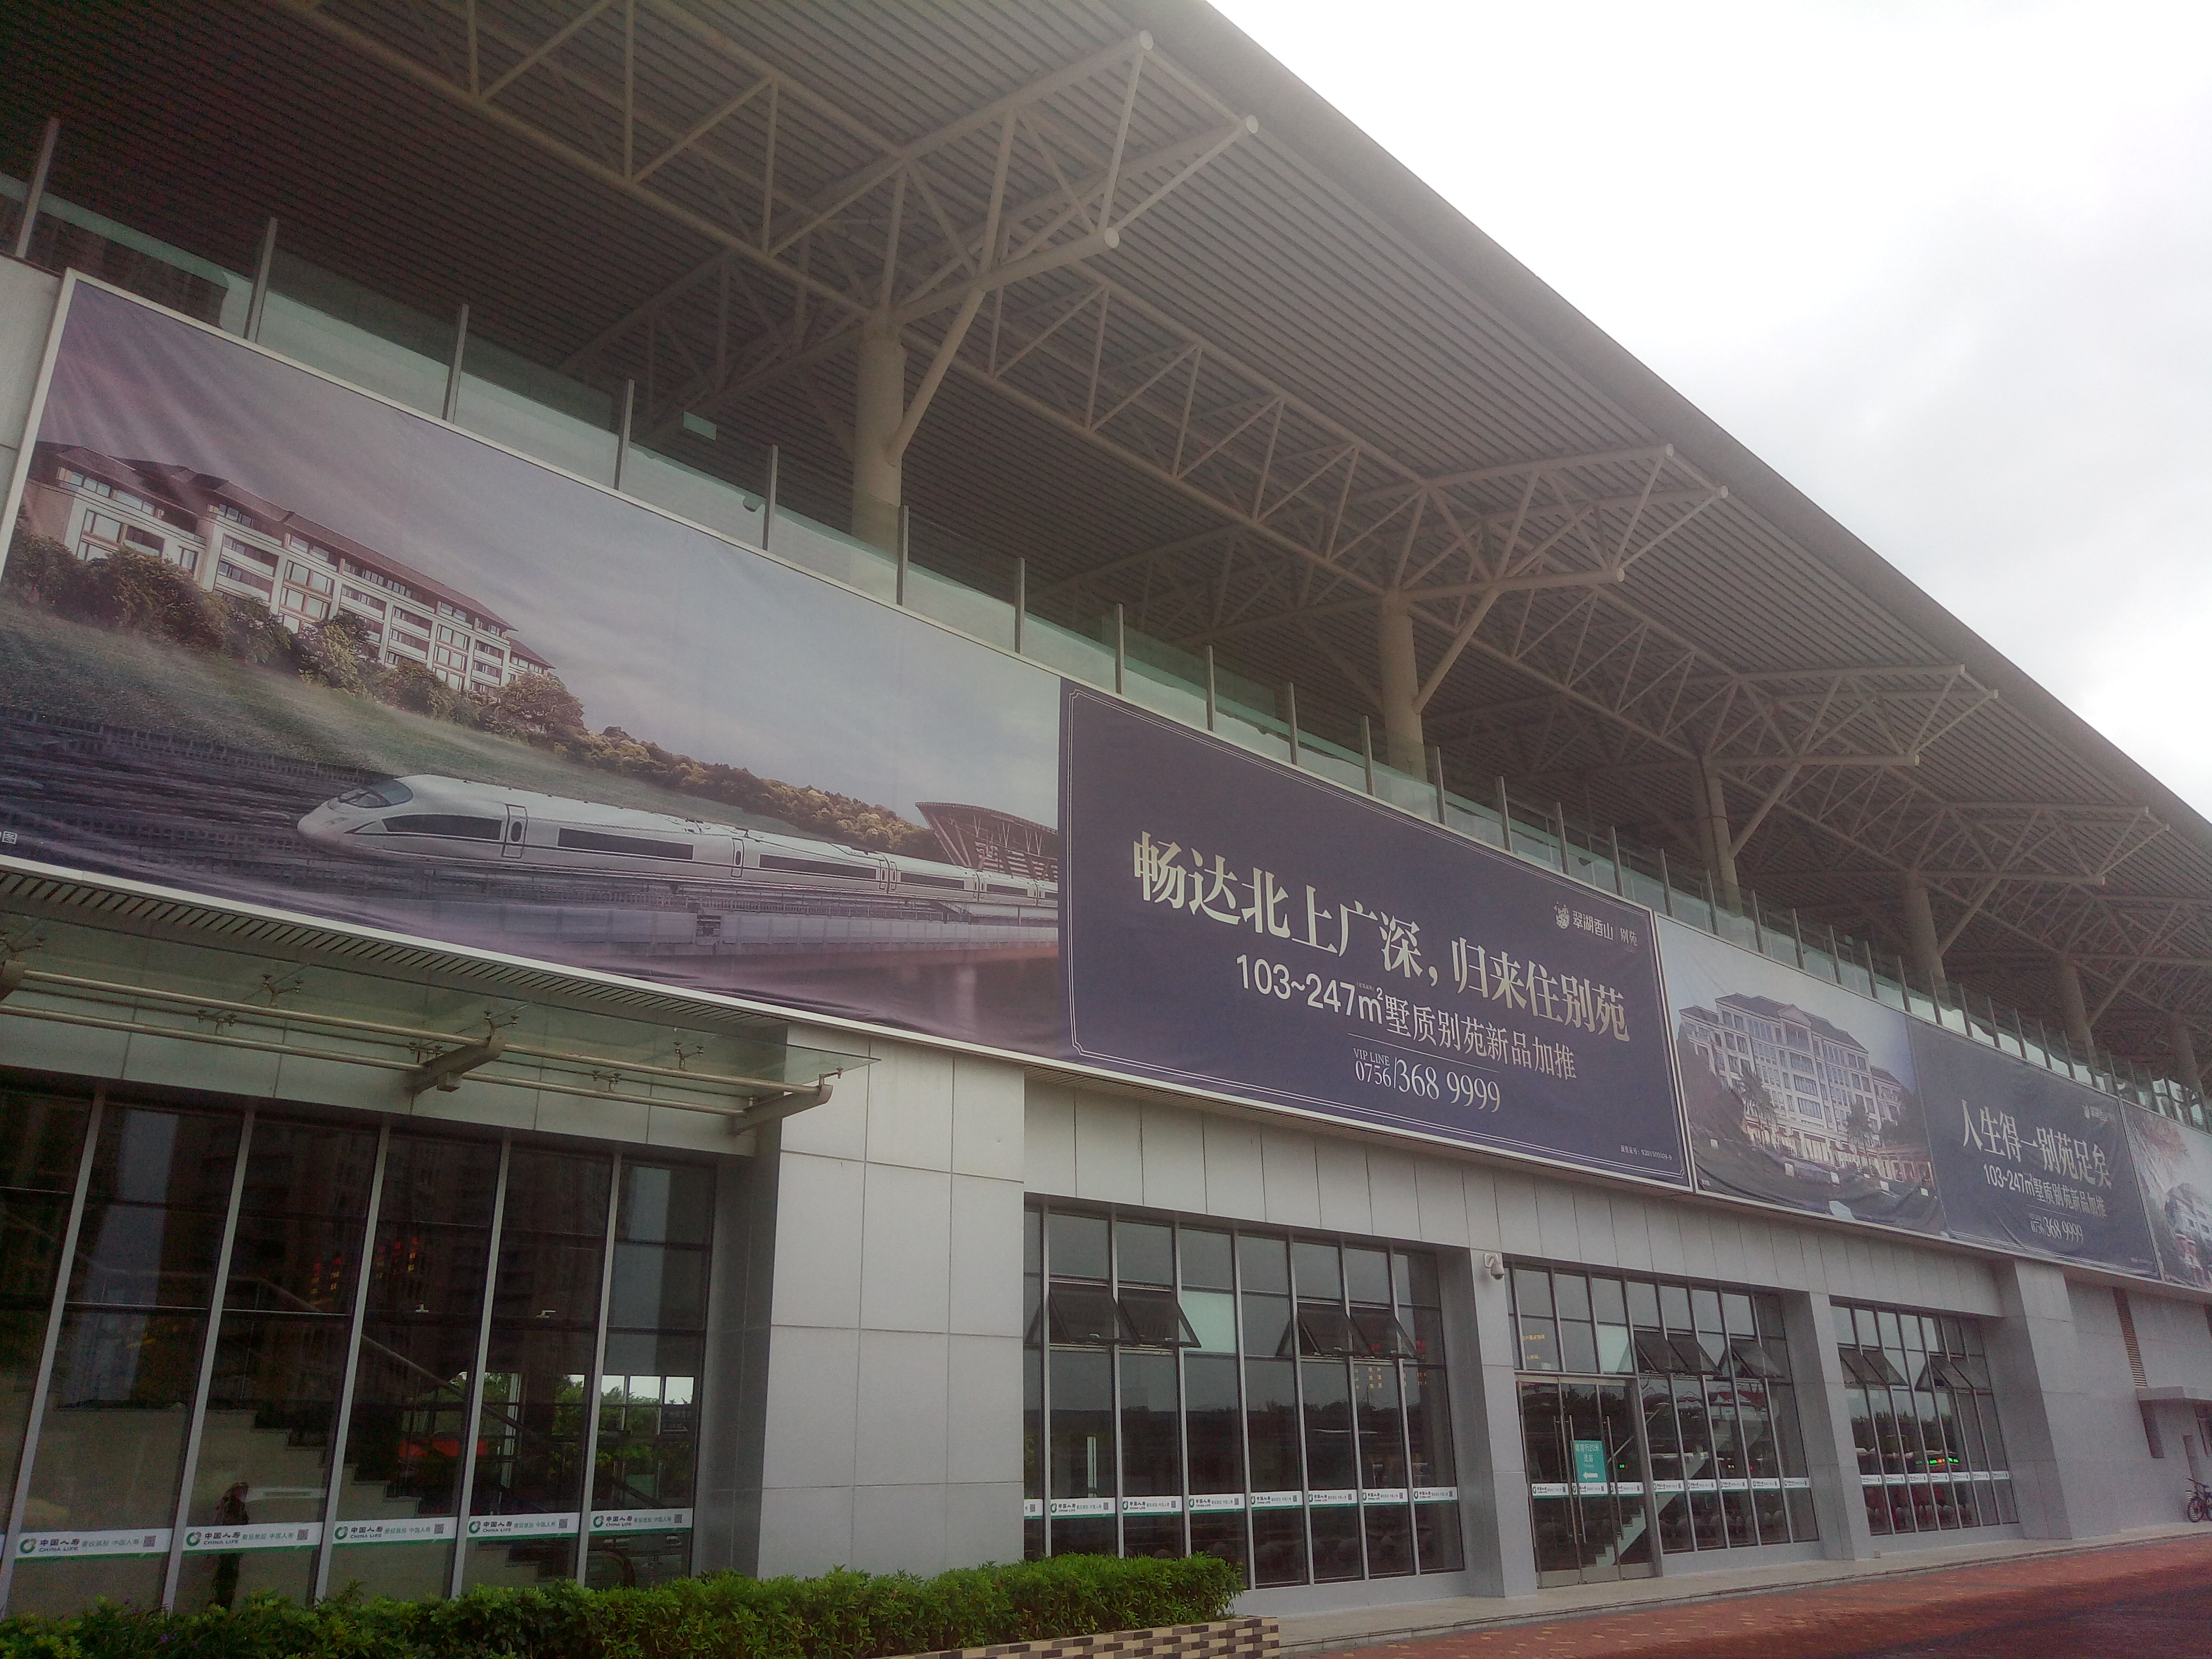
\includegraphics[width=0.48\linewidth]{Figures/Qualitative/tangjia}
	%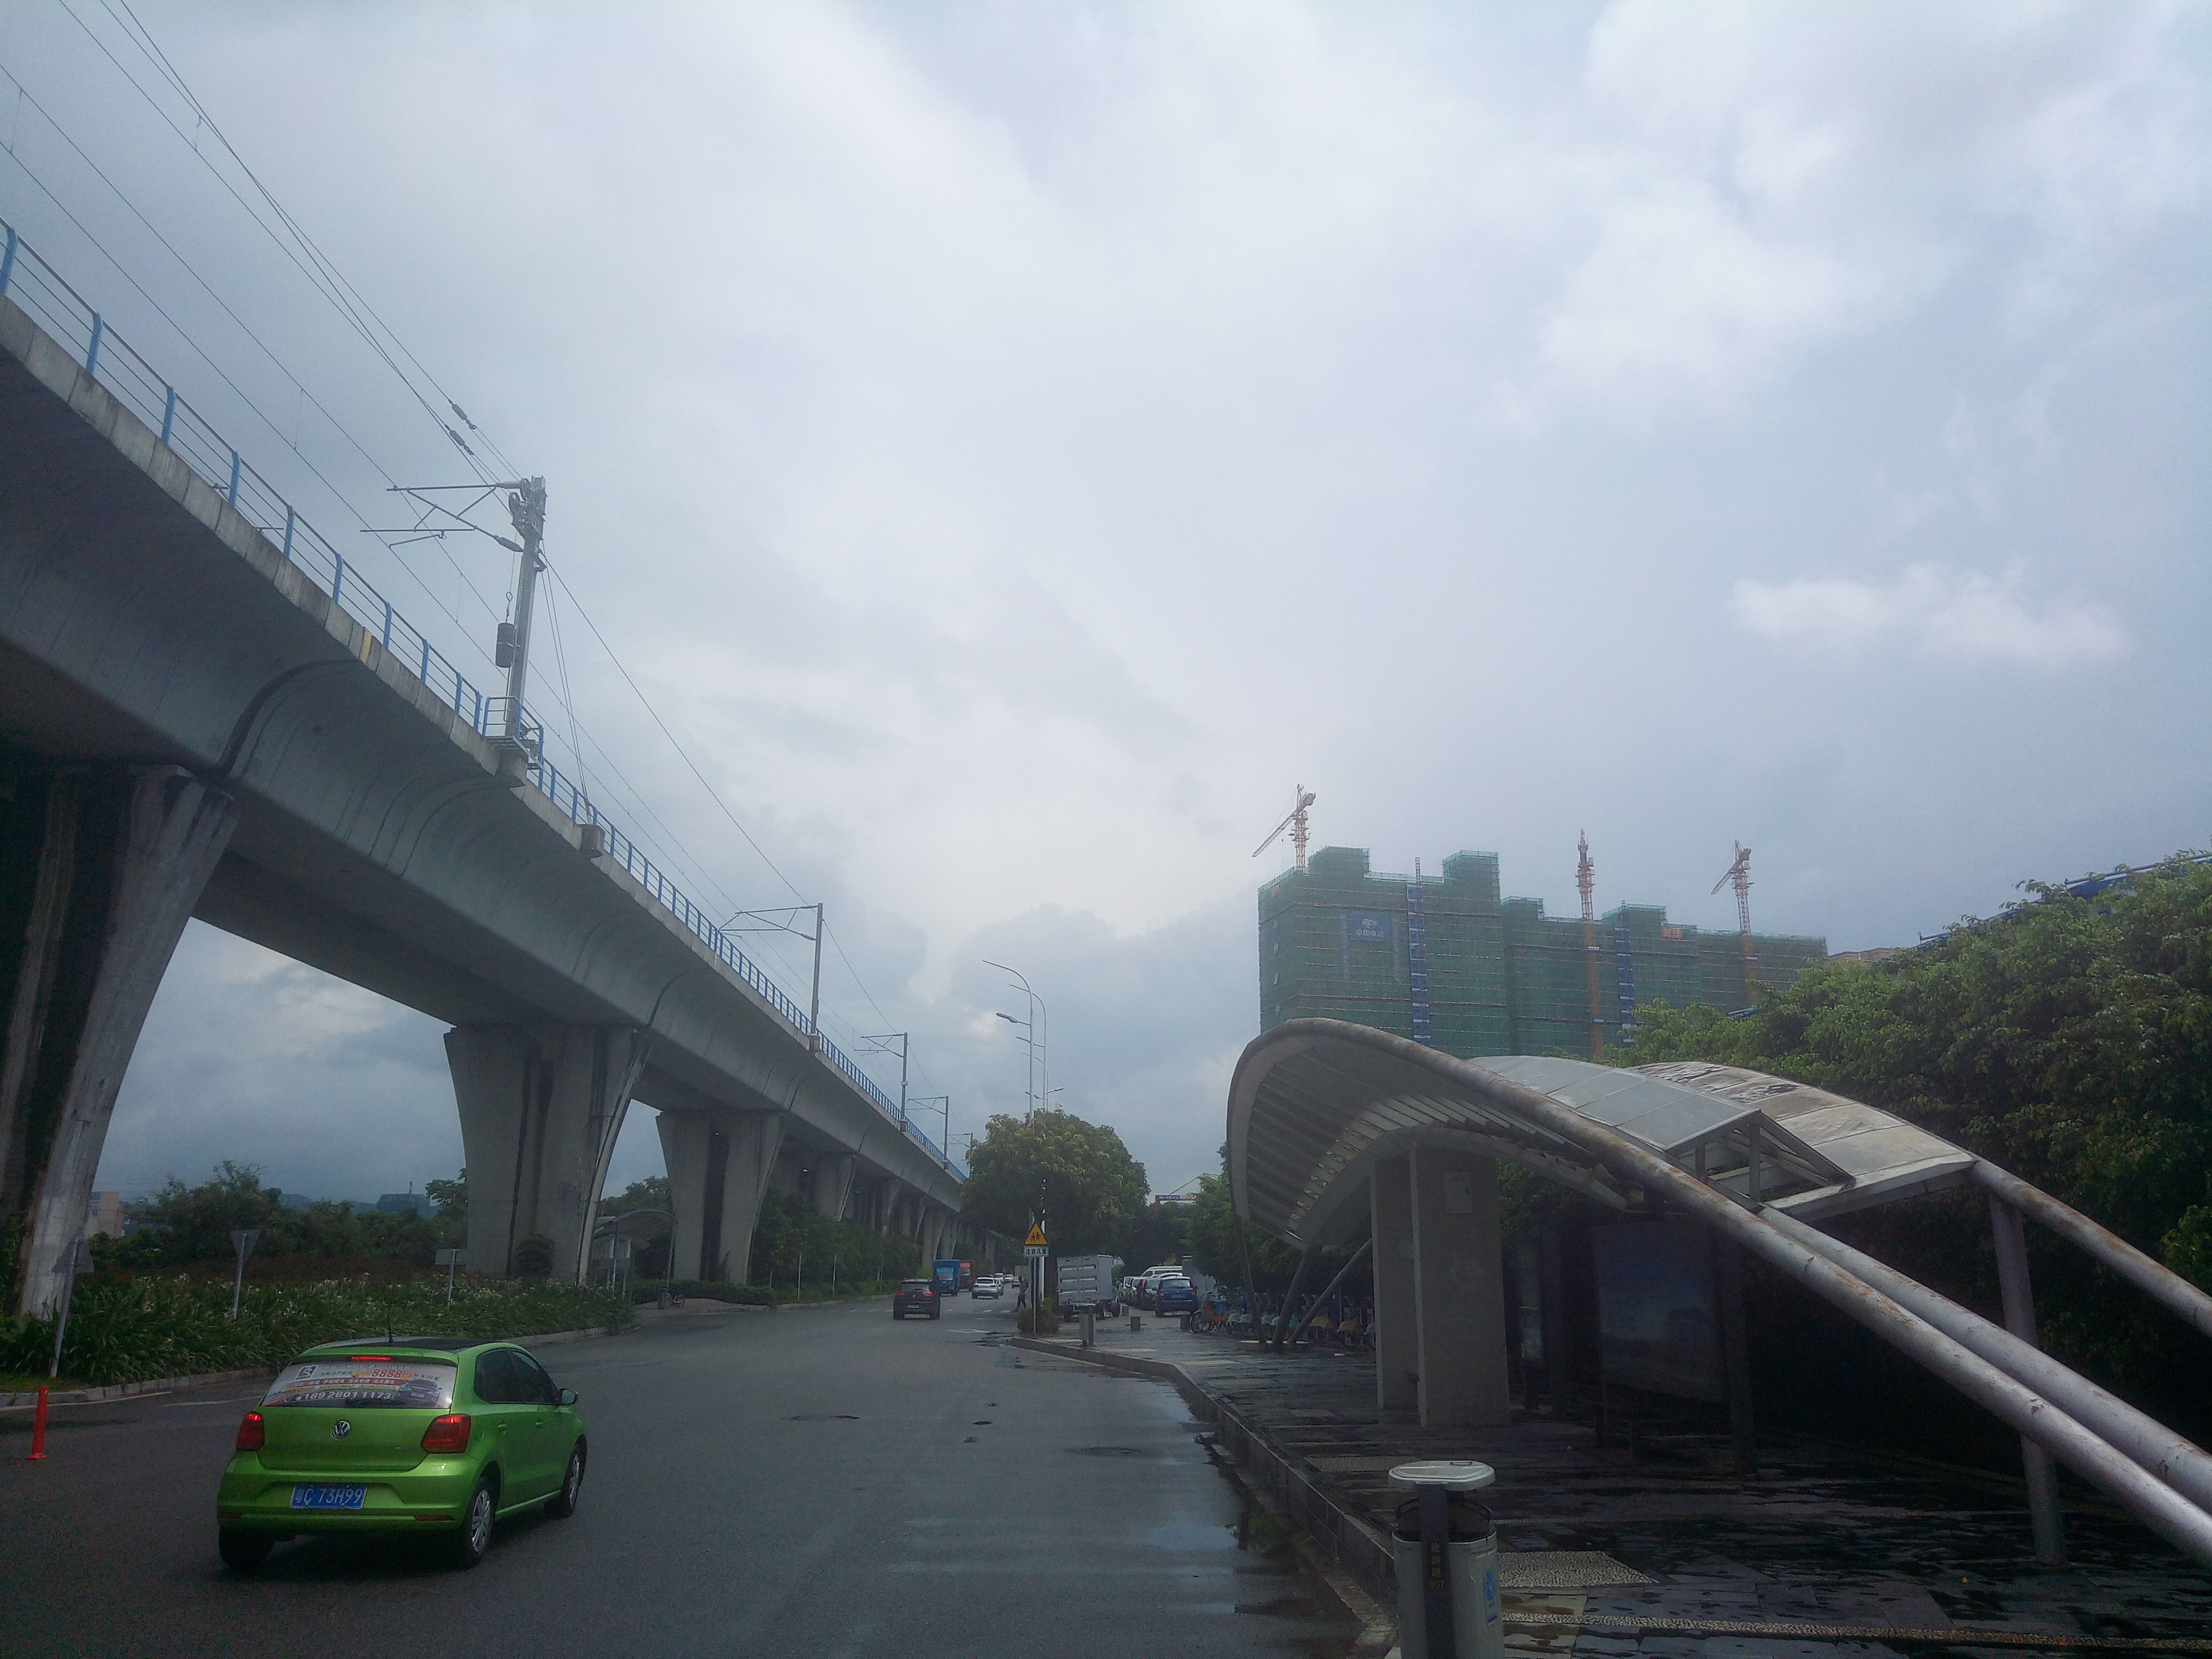
\includegraphics[width=0.48\linewidth]{Figures/Qualitative/zhuhai}\\
	%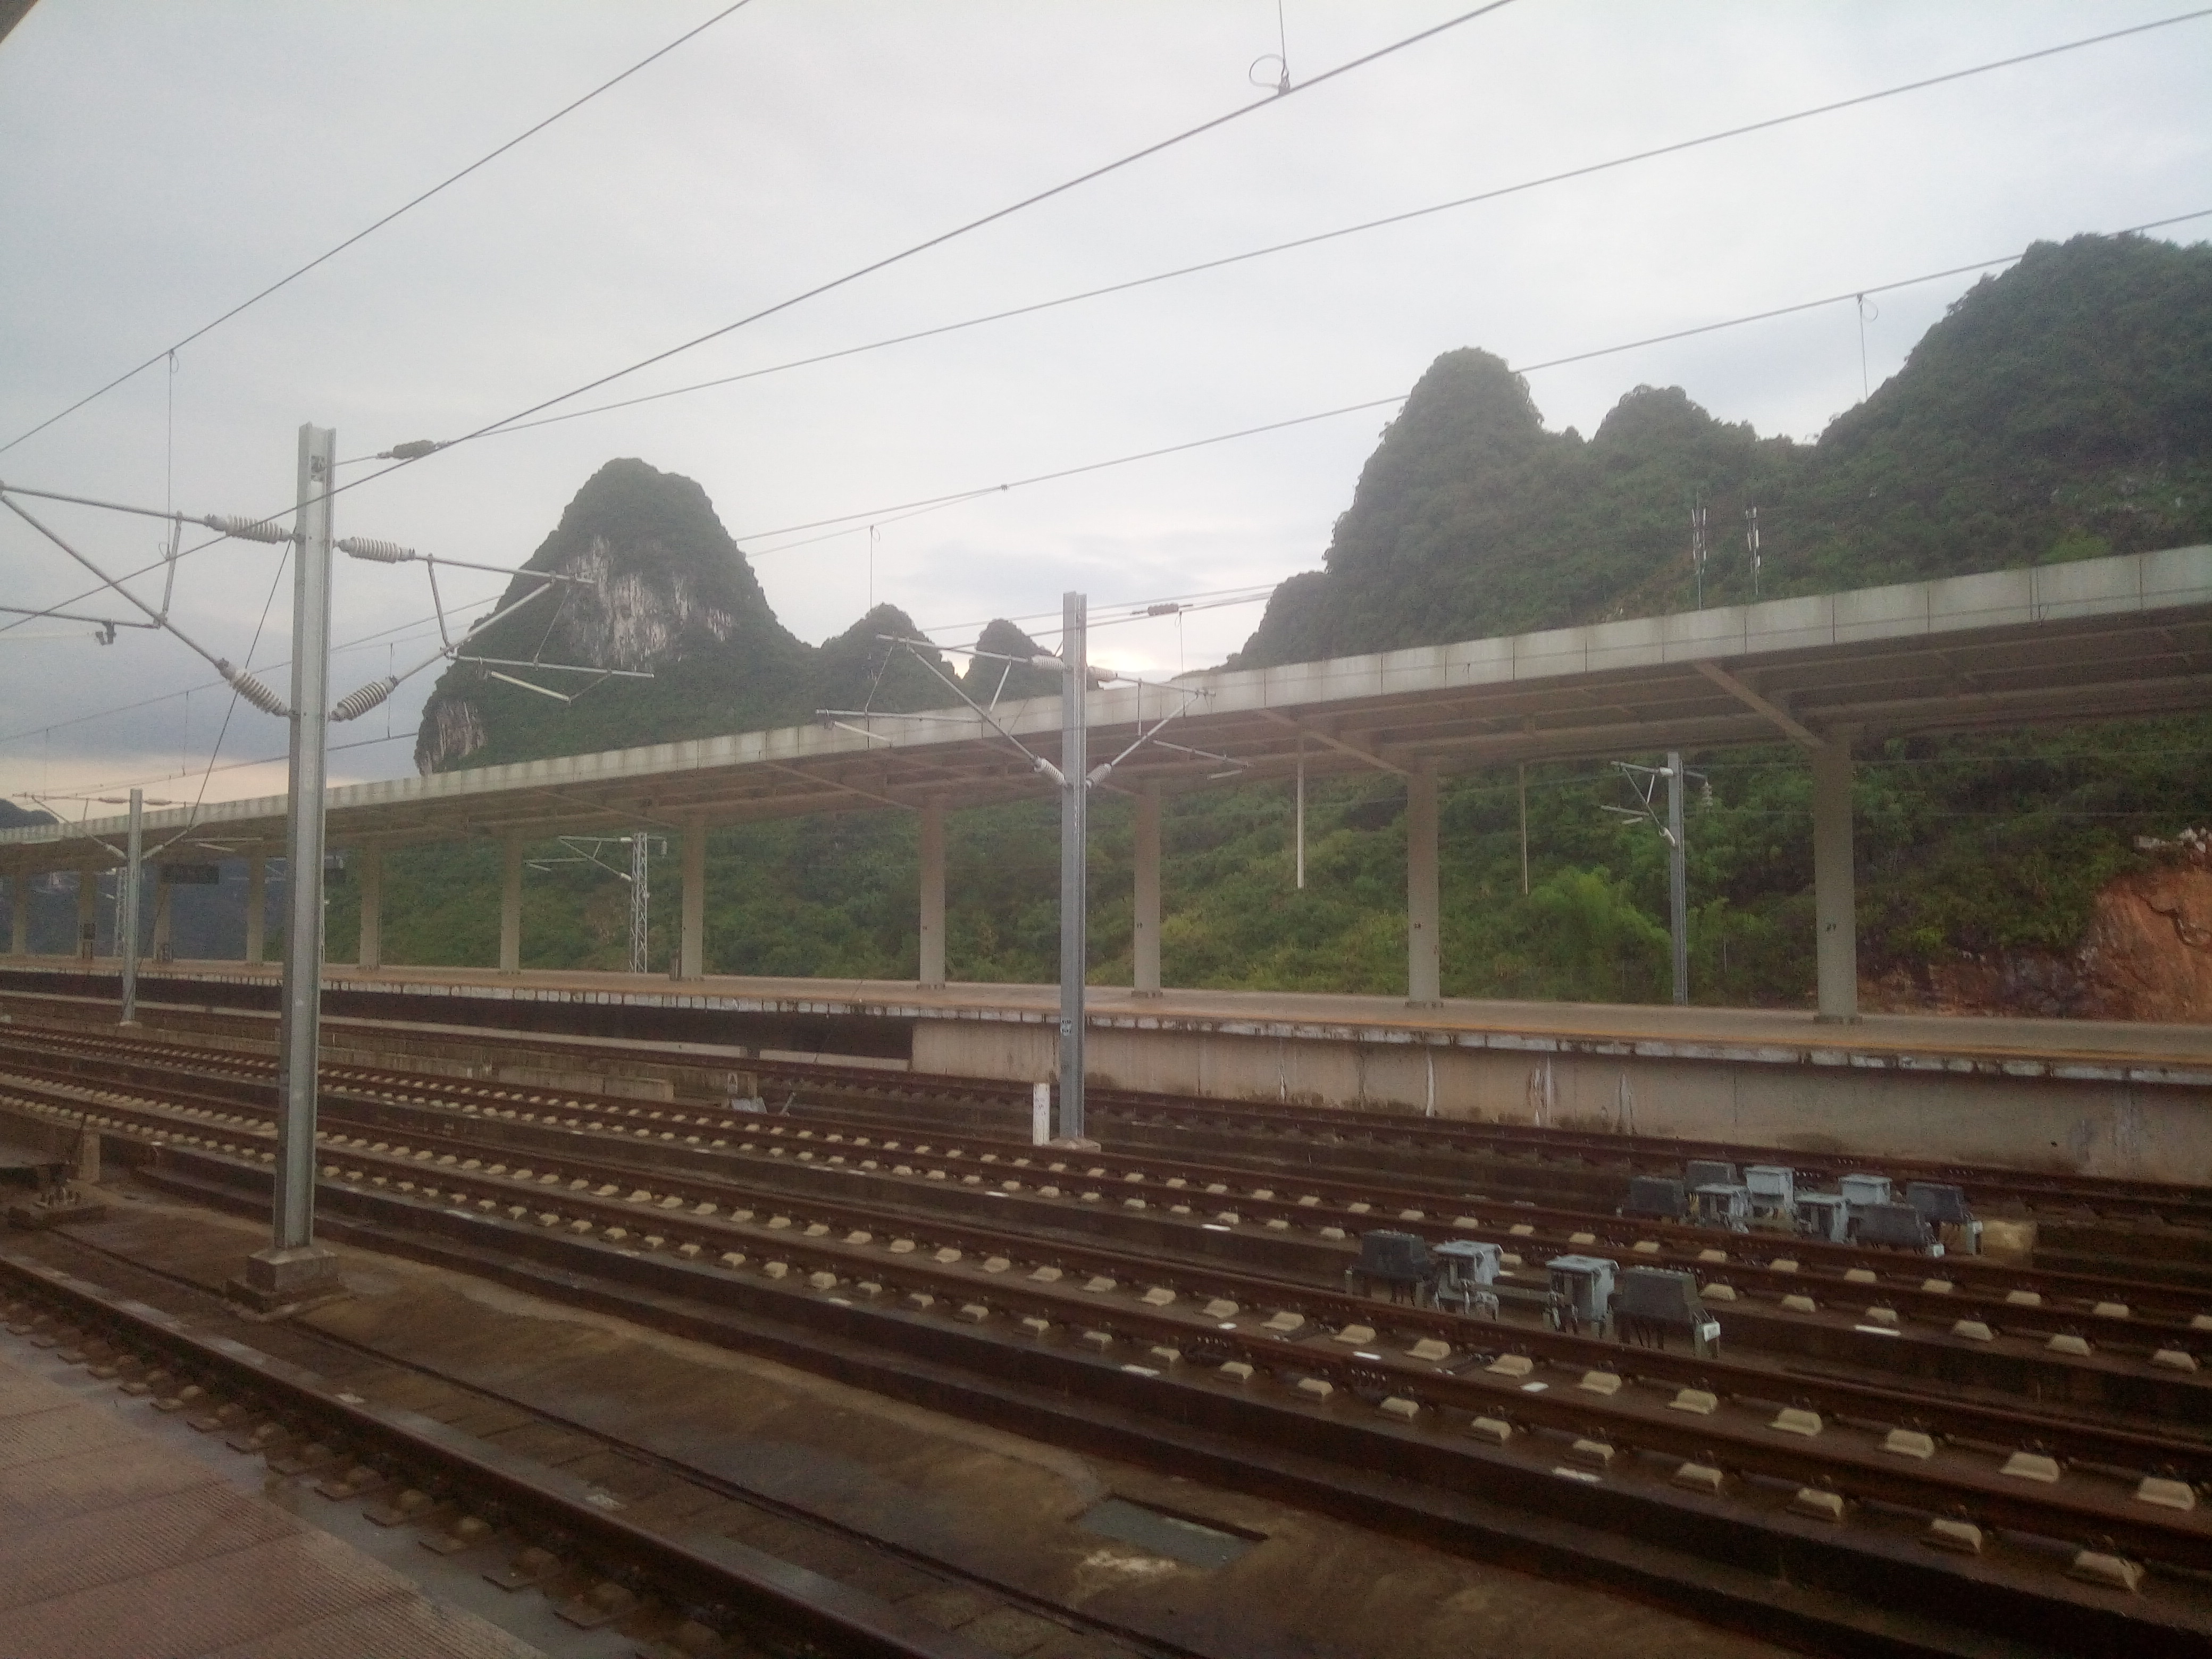
\includegraphics[width=0.48\linewidth]{Figures/Qualitative/yangshuo}
	%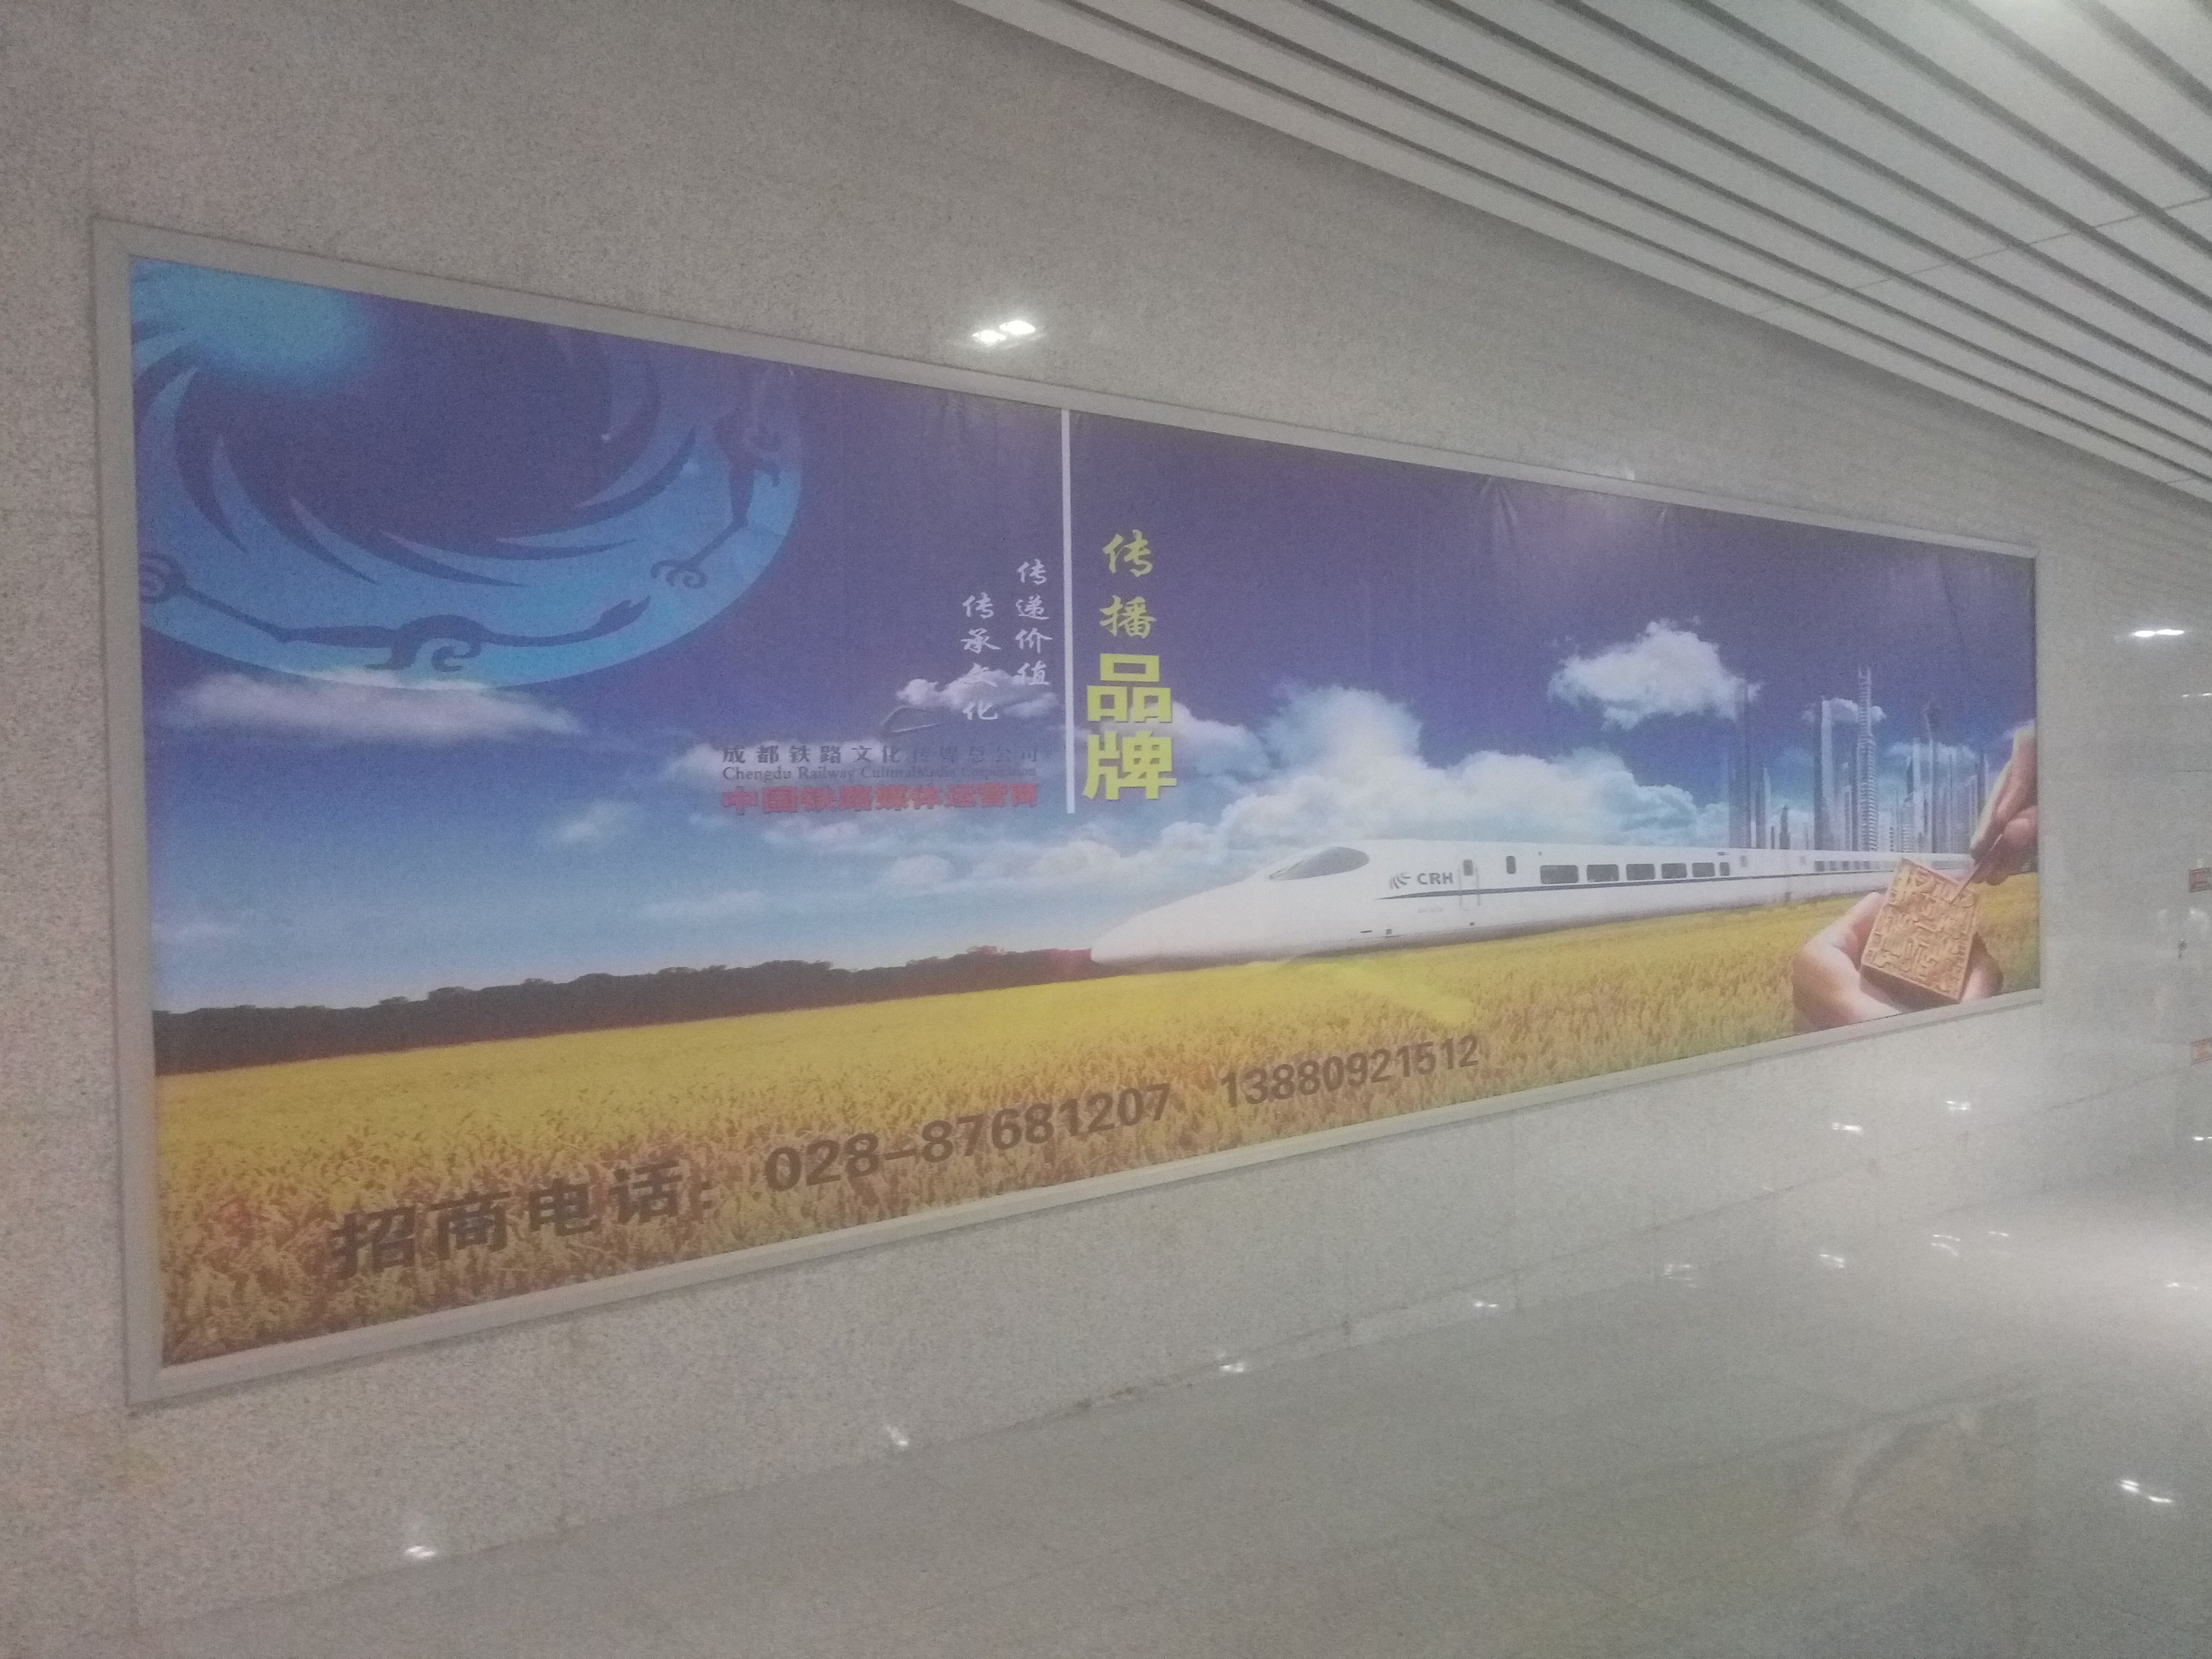
\includegraphics[width=0.48\linewidth]{Figures/Qualitative/chengdu}
	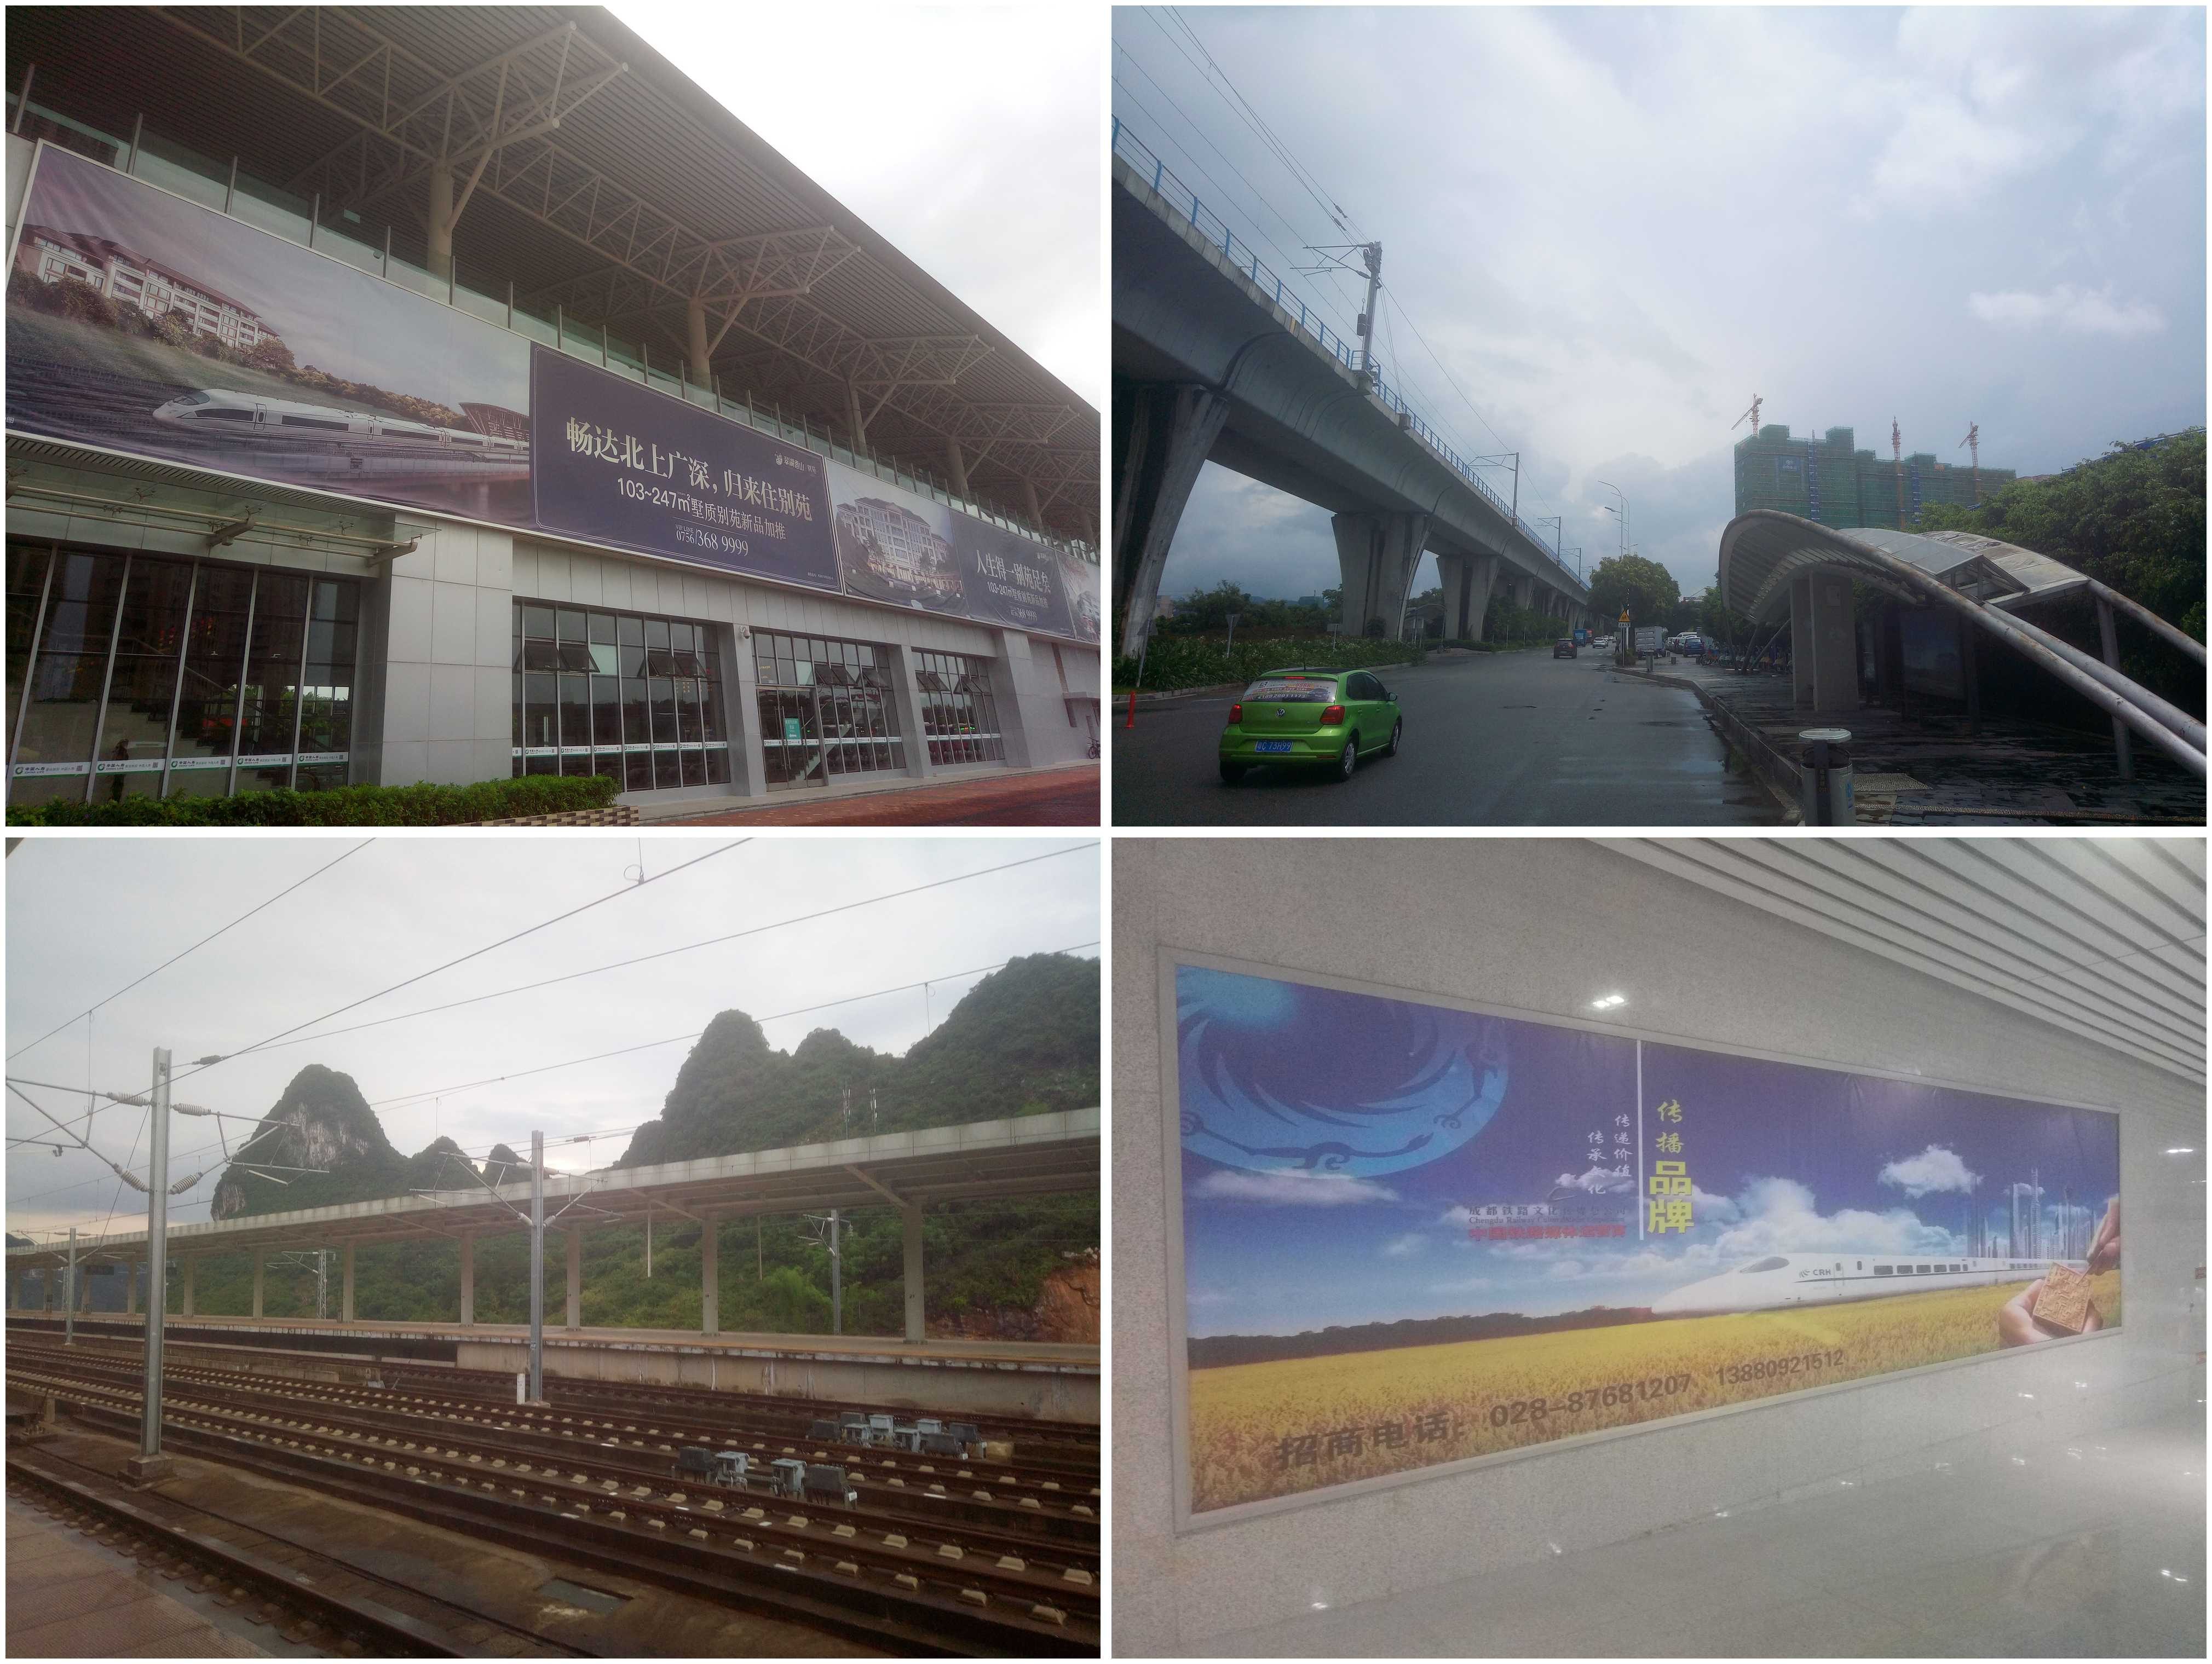
\includegraphics[width=\linewidth]{Figures/Final/1-3-1-fig-qualitative-hsr}
	\caption[][Réseau à grande vitesse en Chine]{(1)Tangjia HSR station in Zhuhai, with a huge advertisement for real estate suggesting the importance of the train connection, what can also be used as an argument for higher prices  (2) HSR line in Zhuhai, deserted bus station and new real estate project in a difficultly accessible area  (3) Yangshuo station, in the middle of nowhere on the High-speed line, recalling the “betterave-TGV” stations typical to France (4) Advertisement for HSR in Sichuan, at Chengdu international airport station on the line to Leshan and Emeishan. \label{fig:qualitative:hsr}}{\textbf{Manifestations locales des mutations induites par le nouveau réseau à grande vitesse.} \textit{(Haut Gauche)} Gare à grande vitesse de Tangjia, sur la commune de Zhuhai. La publicité monumentale pour une opération immobilière vante les mérites d'une proximité au réseau, qui est également utilisée comme un argument pour des prix plus élevés ; \textit{(Haut Droite)} Ligne à grande vitesse à Zhuhai, arrêt de bus déserté et projet immobilier en cours de réalisation dans une zone difficilement accessible\comment[FL]{difficile de comprendre le sens} ; \textit{(Bas Gauche)} La gare de Yangshuo, au milieu de nulle part \comment[FL]{trop rapide voir etudes sur les gares TGV en Espagne} sur la ligne à grande vitesse, rappelant les gares type ``betterave-TGV'' typiques en France ; \textit{(Bas Droite)} Publicité pour la grande vitesse dans le Sichuan\comment[FL]{quel rapport avec le developpement urbain ?}, à la gare de l'aéroport international de Chengdu sur la ligne vers Leshan et Emeishan.\label{fig:qualitative:hsr}}
\end{figure}
%%%%%%%%%%%%%






%%%%%%%%%%%%%%%%%%%%%
\subsection{Implementing TOD: contrasted illustrations}{Implémentation du TOD : des illustrations contrastées}


\bpar{
Regional branches such as the Guangzhou-Zhuhai line can be interpreted in-between a long distance service and regional proximity transportation, depending on the modulation of stop distribution. On top of that still exists the classical train network, and some connections require for now to use both and urban transportation, such as Zhuhai-Hong-Kong that I experimented by terrestrial transport only. The local urban network and real estate development operations are planned in close conjunction with the new train network : Zhuhai new tramway, of which a single line is today open and in test, aims at participating to a ``Transit-oriented development'' (TOD) approach of Urban Development which aims at promoting the use of public transport and a city with less cars, as claimed for example by the High-Tech Zone planning committee in charge of the development around Zhuhai North station. Observing the surroundings of Tangjia station, also constructed in the same spirit, the anti-urban atmosphere and unpractical setting can lead to question the effectiveness of the approach and wonder if it is not more a kind of self-fulfilling prophecy, as suggested by the advertisements for new real estate to sell highlighting the role of the train line. Other field observations, such as in Hong-Kong new territories, witness of an efficient and well achieved TOD, with the smart combination of heavy transit and local light rail, together with high urban densities around stations. These observations recall the complexity of urban trajectories coupled with network development, and how one must be careful before drawing any general conclusion from particular cases.
}{
Des branches régionales\comment[FL]{sens ?} du nouveau réseau à grande vitesse, comme la ligne Guangzhou-Zhuhai, peuvent être vues comme à l'intermédiaire entre un service a longue distance et un transport régional de proximité\comment[FL]{et alors ?}, en fonction de la modularité des motifs de desserte. A cela s'ajoute le réseau de train classique, et certaines connexions requièrent l'utilisation des deux réseaux et des transports urbains, comme la liaison entre Zhuhai et Hong-Kong expérimentée par voie terrestre seulement\footnote{à la suite du Typhoon Hato le 23/08/2017, les liaisons maritimes ont été interrompues pour une grande partie du delta.}. Le réseau urbain local et les opérations de développement immobilières sont planifiés en étroite conjonction avec le nouveau réseau de train : le tramway de Zhuhai, pour lequel une unique ligne est aujourd'hui ouverte et en phase de test, vise a participer à une approche par ``Transit-oriented Development'' (TOD)\footnote{voir les travaux préliminaires de consultation pour la planification, comme par exemple \url{https://wenku.baidu.com/view/b1526461ff00bed5b8f31d01.html} pour le contexte du nouveau quartier de Xiaozhen} du développement urbain qui vise à favoriser l'utilisation des transports publics et une ville avec moins d'automobiles, comme voulu par exemple par le Comité de Planification de la \emph{High-Tech Zone} en charge du développement autour de la gare nord de Zhuhai. L'observation des alentours de la gare de Tangjia, également construite dans le même esprit, une certaine atmosphere anti-urbaine\comment[FL]{sens ?} et une organisation peu pratique peut mener au questionnement de l'efficacité de l'approche et a des interrogations sur la nature auto-prophétique du projet, comme suggéré par les publicités pour du nouvel immobilier a vendre, \comment[AB]{pas très comprehensible} appuyant sur l'importance de la presence de la ligne ferroviaire. Toute une narration autour du TOD, parfois sans réel fondement empirique\comment[FL]{qu'est ce qu'il pourrait y avoir comme fondement empirique ?} dans le cas donné, semble être utilisée par différents acteurs du développement. D'autres observations de terrain, comme dans les Nouveaux Territoires (\emph{New Territories}) à Hong-Kong, témoignent d'un TOD efficace et réalisant son objectif, avec une complémentarité entre transport lourd et tramway local léger, ainsi qu'une grande densité urbaine autour des gares. Ces observations rappellent la complexité des trajectoires urbaines couplées au développement du réseau, et qu'il s'agit d'être prudent avant de tirer toute conclusion générale a partir de cas particuliers. Nous résumons en Fig.~\ref{fig:qualitative:schema} la comparaison des deux cas de TOD évoqués ci-dessus, sous forme de schéma synthétique des grandes lignes urbanistiques de chacune des zones. A Hong-Kong, les zones urbaines ont été planifiées conjointement\comment[FL]{cette discussion est pertinente mais il faut justifier (?)} avec la ligne du MTR (transport lourd) et les multiples lignes de tramway léger, dont l'infrastructure et l'organisation des missions permettent de rejoindre rapidement la gare la plus proche, distribuant une accessibilité très uniforme pour l'ensemble des quartiers du territoire. Au contraire à Zhuhai, le village de Tangjia est ancien, antérieur même à l'ensemble du reste de Zhuhai, qui s'est développé sans articulation particulière avec les infrastructures de transport. Le tracé du tramway, qui vient d'ouvrir, prend avantage du tracé de la nouvelle ligne ferroviaire, pour essayer de reorganiser le nord de Zhuhai\comment[FL]{un peu simpliste}, et en particulier la High-tech Zone qui s'étend de la gare du Nord (Zhuhai Bei) à Tangjia. Actuellement, l'organisation urbaine porte toujours les stigmates \comment[FL]{sens ? (concretement ?)} de cette mise en place déphasée, et l'accessibilité en transport en commun est relativement faible, les lignes de bus étant sujettes à une congestion croissante due à la forte augmentation du nombre d'automobiles. Cet exemple de terrain nous démontre ainsi que (i) sous la même qualification existent des processus très différents, extrêmement dependants aux particularités géographiques, politiques, économiques ; et que (ii) la mise en place d'un territoire fonctionnel en termes d'accessibilité nécessite une articulation fine qui semble résulter d'une approche de planification intégrée réalisée sur le temps long.
}



%%%%%%%%%%%%%
\begin{figure}
	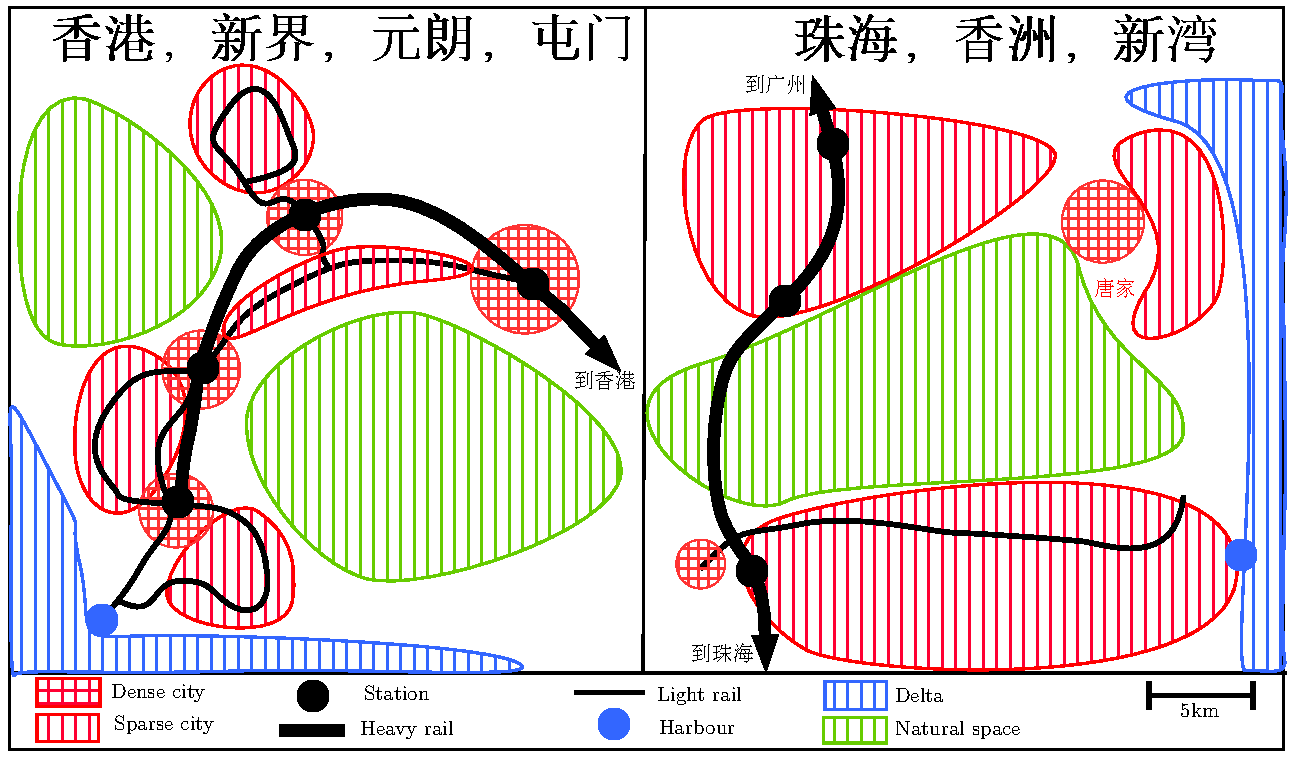
\includegraphics[width=\linewidth]{Figures/Qualitative/tod}
	\caption[TOD in Hong-Kong and Zhuhai][TOD à Hong-Kong et Zhuhai]{\textbf{Comparative analysis of two implementations of TOD in PRD.}\label{fig:qualitative:schema}}{\textbf{Analyse comparative de deux implémentations du TOD \comment[FL]{si ca jour un role important dans ton discours, tu dois le definir}[(JR) fait en 1.1] en PRD.} A une échelle comparable, nous synthétisons la configuration urbaine de Yuenlong (\cn{元朗}) et Tuenmun (\cn{屯门}), Hong-Kong New Territories (\cn{香港,新界}), et de Xinwan, Xiangzhou, Zhuhai (\cn{珠海,香洲,新湾}), qui contient la High-Tech zone de Zhuhai dans sa partie nord en particulier. Les configurations témoignent de dynamiques d'articulation différentes, et des temporalités de construction décalées, révélant ainsi diverses réalités sous la notion de TOD. Une première interprétation serait que celle-ci est efficace si la trajectoire du système territorial complet (aménagement urbain et réseau de transport) est infléchie tôt dans sa genèse, tandis qu'un système avec un certain niveau de maturité sera plus inerte.\label{fig:qualitative:schema}\comment[FL]{traduire la carte ; traduire ; }\comment[AB]{$\rightarrow$ realisation : x ?}}
\end{figure}
%%%%%%%%%%%%%




%-------------------------

%%%%%%%%%%%%%%%
%\subsection[Floating Observation][Observation Flottante]{An Experiment in Floating Observation}{Une Experience en Observation Flottante}
\subsection{Floating Observation}{Observation Flottante}


\bpar{The devil is in the details, and transportation systems are a typical embodiment of this image. What some will see as detail contains the majority of information for others. Logically trapped in a scientific information bubble, despite all the positions developed in introduction, we must stay aware of the nature and the range of knowledge produced here. What can be called detail in our case, for an accessibility study of a transportation network for example, such as subjective views of users or social relations inducted by the situations consequent to the dynamics of the transportation system, will be at the center of the questioning for some viewpoints in anthropology or sociology. Such knowledge, that could surely find a way in our work, is out of scope because of the lack of long-time fieldwork. We propose here however to sketch such a qualitative entry, to suggest directions for future research and better understand processes in a concrete way.}{
%Si le diable est dans les détails, les systèmes de transport entre autres sont l'allégorie de cette adage. Ce que certains appellent détail contient la majorité de l'information pour d'autres. Logiquement enfermés dans une bulle scientifique, malgré toutes les volontés développées en introduction, on tâchera de rester conscient de la nature et la portée de la connaissance produite ici. Ce que nous pourrions appeler détail, lors de l'étude de l'accessibilité d'un réseau de transport par exemple, tel des impressions ressenties par les usagers ou les relations sociales induites par les situations découlant des dynamiques du systèmes, seront le centre du questionnement pour un anthropologue ou sociologue. Une telle connaissance, qui trouverait certainement une place dans nos problématiques, est hors de notre portée de par l'absence de terrain de longue durée. \comment[FL]{c'est TB ce que tu ecris \ldots mais a supprimer de la these}
Nous proposons à présent d'ébaucher une entrée qualitative d'un certain type, pour suggérer une façon de compléter nos connaissances et mieux cerner les processus de manière concrète.
}


\bpar{}{
L'entrée prise suit la méthode \emph{d'observation flottante}, introduite à l'interface de l'anthropologie et la sociologie par~\cite{petonnet1982observation}, avec l'ambition de fonder une anthropologie urbaine, au sens de l'étude des comportements humains au sein d'un environnement urbain. Il ne s'agit pas exactement de la même idée que l'anthropologie de l'espace de \emph{Choay}~\cite{choay2009pour} qui explore la direction inverse, c'est à dire le propre des sociétés humaines de façonner l'espace, et la capacité de construire un environnement bâti à différentes échelles par l'architecture et l'urbanisme. Notre contexte méthodologique est le suivant Répondant à un besoin de mouvement que le sédentaire éprouve facilement, le chercheur se place au centre du processus de production de connaissances, nous citons, en ``rest[ant] en toute circonstance vacant et disponible, à ne pas mobiliser l'attention sur un objet précis, mais à la laisser flotter afin que les informations la pénètrent sans filtre, sans a priori, jusqu'à ce que des points de repère, des convergences, apparaissent et que l'on parvienne alors à découvrir des règles sous-jacentes''. Cette méthode peut servir d'étude préliminaire pour fixer des protocoles et grilles précises d'entretien : elle est par exemple utilisée justement au sujet du transport par~\cite{de2012deplacements}. Nous nous en servons dans notre cas comme méthode d'extraction de faits stylisés, afin d'informer des exemples de processus d'interactions directement visibles.
}



\paragraph{Methodology}{Méthode}

\bpar{}{
Les mouvements pendulaires à échelle moyenne\comment[FL]{c'est quoi ?} sont nécessairement vécus d'une façon particulière en comparaison à d'autres lieux géographiques et à d'autres échelles sur le même lieu. Et si une façon d'appréhender des faits stylisés particuliers était alors d'effectuer l'analogue d'une étude de perturbation sur le système, mais en prenant comme référentiel l'observateur lui-même ? Il s'agirait de faire porter un choc sur une situation ``d'équilibre'', puis de se laisser flotter au gré du courant pour appréhender la réaction et certains mécanismes qu'il aurait été difficile de considérer en suivant sa routine. Une expérience naturelle causée par une perturbation des transports (qui en région francilienne est bien courante\comment[AB]{et pas en Chine ? :)}) est un événement provoquant une expérience naturelle, au sens où le chercheur peut capturer des situations et réactions individuelles particulières.\comment[FL]{il y a sans doute une amorce de travail interessant \ldots plutot en dernier chapitre, exploratoire du type ``pour aller au dela''} Notre méthodologie est relativement simple : déambuler dans les transports en commun, avec ou sans but et de manière ou non aléatoire, mais en essayant sur chaque trajet de maximiser les opportunités de mise en situation ou de capture d'évènement, typiquement en évitant un trajet de routine\footnote{Cette contrainte sera respectée dans notre cas pour le Guangdong, mais pas pour l'Ile-de-France.}. La répétition de l'expérience visera également à maximiser la couverture spatiale, temporelle, de situation. Une production traçable est en théorie nécessaire à chaque itération, qu'il s'agisse de description factuelle, de description perçue, de semi-synthèse. Celle-ci permet a posteriori de voir les stratifications successives du vécu et des expériences d'observation progressivement raffinées dans leur contexte, et de tracer ainsi la genèse des idées induites. Nous faisons le choix de retranscrire l'aspect subjectif, voir maximiser celui-ci dans les synthèses générales des observations, afin d'appuyer cet aspect en contraste avec la suite de notre travail qui sera relativement déconnecté du sujet menant la recherche, et en echo avec les recommandations de \cite{ball1990self} pour la place de la subjectivité dans la recherche ethnographique de terrain.
}




%%%%%%%%%%%%%%%%%%%
\begin{figure}[h!]
\begin{mdframed}
Le ciel est gris et les visages fermés, Oxmo \comment[AB]{est-ce une figure de style? je ne comprends pas bien le principe sinon: c'est bien toi qui flotte non ?} avait tristement raison, ce Soleil du Nord n'avait de lumière que le nom. L'initié ne saura s'y tromper et ressentira au fond de lui-même cette banale routine d'un aller-retour quotidien en RER. Il ne cherchera ni à maudire les planifications successives dont les stratifications temporelles ont laissé décanter cette organisation territoriale incongrue, ni à se prendre à rêver d'une trajectoire de vie alternative puisque choisir c'est un peu mourir et qu'il ne se sent pas une âme de Phoenix aujourd'hui. Peut être que la beauté de la ville est finalement dans ces tensions qui la façonnent à tous les niveaux et dans tous les domaines, ces paradoxes qui deviennent cadre de vie au point d'asséner quotidiennement une vérité. Cette philosophie de couloir de métro, le francilien en fait son cheval de bataille car après tout s'il vit en ville il doit bien la connaître. Encore un rail cassé sur le A, ``tout cela est mal géré, et ce réseau est mal conçu'' vocifère un utilisateur journalier, s'improvisant expert en planification ; d'autres plus patients prennent leur mal en patience mais se présentent tout aussi connaisseurs d'une illusoire vision d'ensemble d'un territoire aux multiples visages. Ces usagers \emph{sont} pourtant le système, de manière concrète à leur échelle d'espace et de temps, par induction et émergence aux échelles supérieures. La fourmi est supposée ne pas avoir conscience de l'intelligence collective dont elle est une des composantes fondamentales. Ils n'ont de la même manière que peu de perception de l'auto-désorganisation dont ils sont la source, peut-être la cause, et qui très sûrement subissent les désagréments de ses dynamiques. Se laisser flotter dans les transports franciliens est une expérience intemporelle. Presque thérapeutique parfois, quand l'un commence à perdre son optimisme quant à l'intérêt d'une vie urbaine, une excursion aléatoire en métro rappelle rapidement la richesse et la diversité qui sont un des plus grand succès des villes. C'est cette variété apparente de profils que le chercheur retiendra principalement de ces errements dont la méthodologie est de ne pas avoir de méthodologie\comment[FL]{non : il y a quelque chose derriere}, et il gardera à l'esprit qu'il n'existe pas d'échelle où un traitement spécifique de chaque objet géographique n'est pas nécessaire : en quelque stations sur la ligne 4 le profil des quartiers et donc des usagers\comment[FL]{attention a ce racourci glissant (tres)} change profondément et souvent sans transition au moins trois fois, comme sur la ligne 13 nord où les motifs horaires soulignent d'autant plus de dures réalités socio-économiques qui sont en fait géographiques dans cet \emph{espace produit} de la métropole. Lorsqu'il s'agit de modéliser, prendre en compte les limites de toute tentative de généralisation est d'autant plus cruciale comme chaque modèle est un équilibre fragile entre spécificité et généralité.\comment[FL]{c'est interessant : a enrichir}

\medskip

\noun{Encadré : } \textit{Une expérience en observation flottante en région parisienne}
\end{mdframed}
\end{figure}
%%%%%%%%%%%%%%%%%%%




%%%%%%%%%%%%%%%%%%%
\begin{figure}[h!]
\begin{mdframed}
Le trajet sera long. La perturbation choisie est la simulation de l'événement malencontreux, ``\cn{我的护照丢了,我得去法国的领事馆在广州}'' \comment[FL]{tu n'es pas aidant avec le lecteur}: la perte de son passeport en Chine est assurément malencontreuse, puisque l'intégralité des trajets interurbains y est conditionnée. Traverser la mega-région urbaine du sud vers le nord pour rejoindre Guangzhou dans cette situation relève du défi. De bus urbain en bus urbain, des terminus plus ou moins bien articulés. Un village traditionnel factice est sorti de terre pour faire le bonheur des touristes, non loin de la maison natale de Zhongshan, peu crédible vu l'accessibilité. Des contrastes saisissants et un paysage très hétérogène, des enclaves de pauvreté dans des zones nouvellement prisées. Les relocalisations plus ou moins volontaires vers les franges façonnent un nouveau paysage d'inégalité géographique que l'on connait déjà bien en Europe. A l'image de cet embouteillage continu, la réinvention de la ville déjà bien avancée ici se doit de faire des choix cruciaux pour être l'exemple d'une trajectoire durable. Une résilience impressionnante des usagers à une perturbation majeure, une capacité d'auto-organisation locale rendant fonctionnels des aménagements qui auraient pu ne pas l'être : de Shenzhen, Baoan à Zhuhai, Tangjia ou à Zhongshan, Xiaolan, la flotte de moto-taxis informels sauve l'accessibilité locale, comme me le confirme Jingzi habitant le sud de Zhongshan et étudiant au nord de Zhuhai et pour qui le train est une solution de mobilité même pas envisagée. Du tramway au BRT, choix et compromis équivalents ? Le premier étonne plus les nouveaux usagers. Peut être aussi un argument percutant pour valoriser le complexe spécialement conçu autour du terminus. Les choix locaux sont d'autant plus différentiables qu'il est difficile de passer d'une zone à l'autre. Bloqué non loin de Guangzhou, le pont est fermé, le métro est en face mais impossible de le rejoindre. Juste le temps pour se rabattre sur la gare de Xiaolan et retour à la case départ, défi bien loin d'être réalisé. Observer l'adaptabilité ne suffit pas à la développer ? Des pratiques de mobilité très vite adaptées par les usagers : des trains à grande vitesse bondés en toute heure de la semaine, semble-t-il pour des motifs très divers. Un développement territorial apparent, des impacts à moyen terme qu'on peut parier non discutables. Si la structure est intégrée et flexible, discuter d'effets structurants devient une tautologie puisque la trajectoire du système urbain devient alors l'aspect plus ou moins contrôlable, selon les échelles de temps et d'espace.


\medskip

\noun{Encadré : } \textit{Une expérience en observation flottante, Guangdong, Zhuhai}
\end{mdframed}
\end{figure}
%%%%%%%%%%%%%%%%%%%



\paragraph{Results}{Résultats}

Nos séquences d'observation de terrain ont eu lieu d'une part en Chine, majoritairement dans le Guangdong à Zhuhai, lors de sessions dédiées. Les observations s'étendent entre le 10/10/2016 et le 23/01/2017 ainsi qu'entre le 08/06/2017 et le 01/09/2017. Le mode de transport majoritaire est le bus de ville, suivi par le train régional, puis le train à grande vitesse et le ferry ; la portée des déplacements correspondent à celle des modes. Les compte-rendus détaillés, écrits à la volée de manière subjective et édités a posteriori le moins possible, comme expliqué précédemment, sont disponibles en Appendice~\ref{app:sec:qualitative}. Les observations pour la région parisienne sont quasi-quotidiennes et non consignées ; celles-ci ont eu lieu en plus grande partie sur la ligne 4 du métro et sur la ligne A du RER entre février 2016 et octobre 2016, sur la ligne R du Transilien et la ligne A du RER entre novembre 2016 et septembre 2017 puis entre février 2017 et mai 2017, puis sur la ligne 9 et la ligne 4 entre septembre 2017 et octobre 2017.

\comment[FL]{ce qui me frappe ici c'est que tu ne parles que de transport et pas de ville ; donc pas de coevolution. pourtant il y a certainement des marqueurs de coevolution a observer de visu (ex gare neuve avec immeubles neufs). D'autre part tu dis ne pas avoir de methode. c'est mal dit, ok pour la demarche ``souple''. par contre tu dois avoir une question, ou au moins des reponses. la tu n'offres pas de cadre de lecture de tes propos.}

Les deux synthèses d'observation flottante pour chacune des régions, matériaux produit à partir des notes brutes, sont présentées dans les encadrés ci-dessus. Celles-ci illustrent entre autre par des exemples subjectifs certaines instances d'interactions entre réseaux et territoires, majoritairement aux échelles microscopique et mesoscopique, pour des processus touchant à la mobilité. La subjectivité et l'interprétation permet aussi d'extrapoler sur des processus à plus grande échelle, en terme d'accessibilité par exemple. Ceux-ci ne peuvent toutefois être pris plus que comme une illustration et introduction thématique. Par une prise de recul, nous proposons de lister certains enseignements qui peuvent être tirés de cette expérience à un niveau méta :

\begin{enumerate}
	\item La complexité du système de transport et de son intégration dans le système territorial\comment[FL]{tu donnes un angle non symmetrique} peut avoir des conséquences divergentes en termes de performance finale, et par exemple de soutenabilité. Dans le cas Chinois, l'auto-organisation et l'adaptabilité locale sont des atouts de l'efficacité émergente\comment[FL]{defs}, tandis qu'en France la complexité semble être source de freins et finalement d'externalités négatives. \comment[FL]{tres schematique, enrichir}\comment[AB]{différence vient-elle en partie de l'adaptabilité différentielles des populations ? (ie origine culturelle)}
	\item La résilience, qui peut être caractérisée par exemple \comment[FL]{pas d'accord avec ta definition} par la vitesse de mutation des pratiques de mobilité et reliée à l'adaptabilité, semble également très sensible aux particularités géographiques.
	\item La question des échelles de temps et d'espace observables, ce qui conditionnera partiellement celles qu'on peut modéliser, est ambiguë dans l'observation, comme le témoigne l'observation conjointe de la mobilité et de manifestation de motifs d'accessibilité.
	\item La comparabilité des cas et des situations géographiques est, dans notre cas, mais a priori plus généralement, un point épineux auquel il n'existe pas de solution idéale. Le compromis entre généralité et particularité est alors déterminant dans la construction d'une théorie et de modèles géographiques. \comment[FL]{pourquoi soulever cette question ? tu ne fais pas de comparaison dans ta these. par contre une vraie question est la tranposabilite des approches de modelisation d'un territoire a un autre.}
\end{enumerate}


Ces considérations participeront à l'orientation des postures ontologiques et épistémologiques que nous prendrons par la suite.

\comment[FL]{manque litérature ``de base'' sur interactions ville/transport.}

\comment[FL]{transport - territoire : majorite sur transport ?}


\stars





%
% Conclusion





%----------------------------------------------------------------------------------------

\newpage


\section*{Chapter Conclusion}{Conclusion du Chapitre}


Les territoires, que nous avons défini comme territoires humains, interagissent de manière complexe avec les réseaux, en particulier ceux de transport, comme montré par les nombreux exemples empiriques ou les constructions théoriques passés en revue. A différentes échelles temporelles typiques, l'année, la décennie et le siècle, correspondent plus ou moins des échelles spatiales : métropolitaine, régionale et système de villes, ainsi que des processus : mobilité, accessibilité et relocalisations, effets systémiques structurels et bifurcations.\comment[FL]{plus haut} Les situations concrètes témoignent de réalités locales déclinés avec différentes nuances, et des processus portant ces processus abstraits avec différents rôles et interactions entre eux. Nous avons dans une première section clarifié cette notion d'interaction\comment[FL]{pas vraiment : hierarchiser, faire preuve de pedagogie.} entre réseaux de transports et territoires, et suggéré une approche par la co-évolution pour tenir compte de cette complexité. Afin de mieux cerner ces notions sur des exemples géographiques concrets, nous avons développé en~\ref{sec:casestudies} deux cas d'étude métropolitain d'actualité, et souligné les certitudes en termes d'impact d'accessibilité pour des projets majeurs d'infrastructures qui s'accompagnent systématiquement d'incertitude en terme de trajectoire du système à plus long terme. Enfin, pour limiter les effets d'intermédiaire qui augmenteraient la distance au terrain géographique réel qui est selon~\cite{lefort2012terrain} déjà très présente dans les études le prenant comme matériau empirique principal, nous proposons en~\ref{sec:qualitative} une excursion par des éléments de terrain dans le Guangdong, Chine.\comment[FL]{a reprendre} A ce stade, ayant introduit l'objet d'étude thématique, nous proposons de restreindre la portée des entrées prises sur le sujet, et s'intéresser plus particulièrement aux approches impliquant une modélisation, faisant le choix d'un rôle fondamental du \emph{modèle} (que nous définirons par la suite) dans la production de connaissance.





\stars


%-------------------------


% no role here, or put that elsewhere

%\section{Research Question}{Question de Recherche}

%To close this thematic touring introducing chapter, we can state a general research question that frames our further theoretical constructions and first modeling attempts. It is roughly the same as the problematic given at the end of previous section, but adding the insight of modeling as the approach to understand these complex systems.

%networked territorial systems with an emphasize on the role of transportation networks in system evolution processes.

%\medskip

%\textbf{General research Question.} \textit{To what extent a modeling approach to territorial systems as networked human territories can help disentangling complexly involved processes ?}

%\comment{(Florent) à mieux détailler et à réduire d'abord }

%\medskip

%This question will be refined by theoretical developments in the next chapter and experiments in the followings.




%%%%%%%%%%%%%%%%%%%%%%%%%%%%%


%%%%%%%%%%%%%%%%%%%%%%%%%%%%%
% Chapter 2 : Modeling the Interactions


%\chapter{Modeling Interactions between Networks and Territories}{Modéliser les Interactions entre Réseaux et Territoires} % Chapter title
\chapter{Modéliser les Interactions entre Réseaux et Territoires}


\label{ch:modelinginteractions}

%----------------------------------------------------------------------------------------




Si la littérature empirique et thématique, ainsi que les cas d'études développés précédemment\comment[FL]{NB: comme je commence par lire des 2 je ne les ai pas en tete}, semblent converger vers un consensus sur la complexité des relations entre réseaux et territoires\comment[FL]{mots qu'il conviendra d'avoir definis precedemment}, et\comment[FL]{faire deux phrases} dans certaines configurations et à certaines échelles de relations circulaires causales entre dynamiques territoriales et dynamiques des réseaux de transports\comment[FL]{pourquoi dans la premiere partie de la phrase il ny a pas transports et la oui?} que l'on se proposera de désigner par \emph{co-évolution}\comment[FL]{faire une tournure de phrase plus simple pour definir le not coevolution}, ceux-ci semblent diverger sur toute explication potentiellement simple\comment[FL]{mal dit} ou systématique, comme le rappelle par exemple les débats autour des effets structurants des infrastructures~\cite{offner1993effets}\comment[FL]{qu'il convient ici d'expliciter en 2.3 - $\phi$ : qui dit quoi dans ce debat ?}. Au contraire, les multiples situations géographiques poussent à privilégier des études ciblées très fortement dépendantes du contexte et du travail de terrain\comment[FL]{phrase un peu rapide tu donnes l'impression que tu tranches le debat}. Or l'explication géographique et la compréhension des processus est très vite limitée dans cette approche, et intervient un besoin d'un certain niveau d'abstraction et de généralisation\comment[FL]{or justement il convient d'expliciter ce debat theorie vs empirisme (ou autre)$\rightarrow$dans la phrase en pointilles tu parles d'un besoin d'abstraction, ce nest pas le terme scientifique}. C'est sur un tel point que la Théorie Evolutive des Villes se concentre particulièrement\comment[FL]{il faut absolument se departir d'un ton enthousiaste non scientifique. tu te proposes d'appliquer une theorie/un cadre analytique a une question - ca marche plus ou moins, cest tout, il ne doit pas y avoir d'a priori ou de preference de ton cote}, puisqu'elle arrive à combiner des schémas et modèles généraux aux particularités géographiques, et en tire même parti, tandis\comment[FL]{faire deux phrases} que certaines théories issues de la physique comme la Théorie du Scaling de \noun{West}~\cite{west2017scaling} peuvent être plus difficile à digérer pour les géographes\comment[FL]{tu pars deja dans de l'interpretation epistemo : il faut séparer les choses, d'abord de quoi s'agit-il ?} de par leur positionnement d'universalité qui est à l'opposé de leurs épistémologies habituelles. Dans tous les cas, le \emph{medium} qui permet de gagner en généralité sur les processus et structures des systèmes est toujours le \emph{modèle}\comment[FL]{l'italique ne joue pas le meme role pour les 2 mots cela prete a confusion} (voir \ref{sec:knowledgeframework} pour un développement des domaines de connaissance et du rôle du modèle). Comme le rappelle \noun{J.P. Marchand}~\cite{raimbault2017entretiens}, ``notre génération a compris qu'il y avait une co-évolution, la votre cherche à la comprendre''\comment[FL]{TB citation a mettre en italique}, ce qui appuie le pouvoir de compréhension apporté par la modélisation et la simulation qui pourraient être aujourd'hui à leur balbutiements\comment[FL]{ok avec le sens de cette phrase mais le conditionnel sonne mou. si tu as des arguments avance les, sinon dis clairement auelle est ta position}. Sans développer les innombrables fonctions que peut avoir un modèle, nous nous baserons sur l'adage\comment[FL]{terme non scientifique} de \noun{Banos} qui soutient que ``modéliser c'est apprendre'', et suivant notre positionnement dans une science des systèmes complexes suggéré en introduction, nous ferons ainsi de la \emph{modélisation des interactions entre réseaux et territoires} notre principal sujet d'étude, outil, objet (même si dans une lecture rigoureuse de~\ref{sec:knowledgeframework} ce positionnement n'a pas de sens puisque notre démarche contenait déjà des modèles à partir du moment où elle était scientifique\comment[FL]{tu ne peux pas parler d'une lecture rigoureuse de tes propres propos ! supprime la ()}). Ce chapitre peut être vu comme un ``état de l'art'' des démarches de modélisation des interactions entre réseaux et territoires. Il vise en particulier à être aussi objectif et exhaustif que possible\comment[FL]{mal amene, cest souvent le but non ?} : pour cela, nous mobiliserons des analyses en épistémologie quantitative. Dans une première section~\ref{sec:modelingsa}, nous passons en revue de manière interdisciplinaire les modèles pouvant être concernés, même de loin, sans a priori d'échelle temporelle ou spatiale, d'ontologies, de structure, ou de contexte d'application. Les modèles de changement d'usage du sol très appliqués en planification sont tout autant concernés que des modèles totalement abstraits issus de la biologie ou de la physique, que des approches intégrées en géographie ou spécifiques en économie\comment[FL]{pas utile ici tu detailleras en 2.1 : ici affirmer les objectifs (quelle information en retirer) et les moyens (par ez meme automatique tu as bien un (des) points d'entrees $\rightarrow$ lesquels et pourquoi?}. Cet aperçu suggère des structures de connaissances assez indépendantes et des disciplines ne communiquant que rarement\comment[FL]{B}. Nous procédons à une revue systématique algorithmique\comment[FL]{est-ce une facon standard de nommer cela ?}[(JR) l'exploration iterative de la facon dont elle est faite n'a jamais ete faite a ma connaissance, j'introduis donc une ``nouvelle'' façon de faire.] dans~\ref{sec:quantepistemo} pour reconstruire leur paysage scientifique, dont les résultats tendent à confirmer ce cloisonnement\comment[FL]{c'est interessant bien sur mais il faut dire pourquoi tu vises cela. a mon avis il vaut mieux commencer par des exemples de manieres dont la litterature sci. prend en compte ces interactions, dans differentes disciplines, avant d'atteindre l'epistemologie quantitative.}. L'étude est complétée par une analyse d'hyperréseau, combinant réseau de citation et réseau sémantique issu d'analyse textuelle, qui permet de mieux cerner les relations entre disciplines, leur champs lexicaux et leur motifs d'interdisciplinarité. Cette étude permet la constitution du corpus utilisé pour la modélographie et la meta-analayse\comment[FL]{mots qui nont pas encore ete introduits} effectuée en dernière section~\ref{sec:modelography}, qui dissèque la nature d'un certain nombre de modèles et la relie au contexte disciplinaire, ce qui pose les bases et le cadre précis des efforts de modélisation qui seront développés par la suite.






\stars


\textit{Ce chapitre est inédit pour sa première section ; reprend dans sa deuxième section le texte traduit de~\cite{raimbault2015models}, puis pour sa deuxième partie la méthodologie de \cite{raimbault2016indirect}, les outils de \cite{bergeaud2017classifying} et des passages de~\cite{}; et est enfin inédit pour sa dernière partie.}

\comment[FL]{mettre bout a bout tous ces passages (non classiques, mais que je trouve beinvenus, en toute fin d'intro generale)}[à rediscuter, je trouve ca plus adapté pour chaque chapitre dans le cadre d'une ``these a papiers'' (meme si c'est est pas une officiellement).]







%
% 2.1 - State of the Art




%----------------------------------------------------------------------------------------

\newpage

\section{Modeling Interactions}{Modéliser les Interactions}
\label{sec:modelingsa}


%----------------------------------------------------------------------------------------





% -- from algoSR --

%\comment{(Florent) c'est différent de la littérature empirique sur ces interactions}

%\paragraph{Land-Use Transportation Interaction Models}{Modèles LUTI}


%\bpar{
%A wide class of models that have been developed essentially for planning purposes, which are the so-called Land-use Transportation Interaction Models, is a first type answering our research question. See diverse reviews \cite{chang2006models}, \cite{iacono2008models} and \cite{wegener2004land} to get an idea of the heterogeneity of included approaches, that exist for more than 30 years. Recent models with diverse refinements are still developed today, such as \cite{delons:hal-00319087} which includes housing market for Paris area. Diverse aspects of the same system can be translated into many models (as \eg \cite{wegener1991one}), and traffic, residential and employment dynamics, resulting land-use evolution, influenced also by a static transportation network, are generally taken into account.
%}{
%Une large classe de modèle développés essentiellement dans des objectifs de planification, \comment{(Florent) c'est un aspect à part entière mais à mon avis pas dès le début} les modèles d'interaction entre transport de usage du sol, sont un premier type pouvant rentrer dans notre problématique. Voir les diverses revues~\cite{chang2006models},~\cite{iacono2008models} et~\cite{wegener2004land} pour avoir un aperçu de l'hétérogénéité des approches incluses, qui existent depuis plus de 30 ans.\comment{(Florent) seventies}  Des versions récentes avec divers raffinements sont toujours développés aujourd'hui, comme~\cite{delons:hal-00319087} qui inclut le marché immobilier pour la région parisienne. Différents aspects du même système peuvent être traduits par divers modèles (comme e.g. \cite{wegener1991one}), et le traffic, les dynamiques résidentielles et d'emploi, l'évolution de l'usage du sol en découlant, influencée aussi par un réseau de transport statique, sont généralement pris en compte.  \comment{(Florent) description}
%}


%\paragraph{Network Growth Approaches}{Approches de Croissance de Réseau}


%\bpar{
%On the contrary, many economic literature has done the opposite of previous models, i.e. trying to reproduce network growth given assumptions on the urban landscape, as reviewed in \cite{zhang2007economics}. In~\cite{xie2009modeling}, economic empirical studies are positioned within other network growth approaches, such as work by physicists proposing model of geometrical network growth \cite{barthelemy2008modeling}. Analogy with biological networks was also done, reproducing typical robustness properties of transportation networks \cite{tero2010rules}.
%}{
%A l'opposé de nombreux travaux ont pris la logique inverse, i.e. essayent de reproduire la croissance du réseau étant donné des hypothèses sur l'environnement urbain, \comment{(Florent)  sur leurs dynamique, ou bien leur structure, figée ?} comme résumé dans~\cite{zhang2007economics}. Dans~\cite{xie2009modeling}, les travaux économiques empiriques sont positionnés parmi les autres approches de la croissance des réseaux, comme des travaux de physiciens proposant des modèles de croissance géométrique locale~\cite{barthelemy2008modeling}. L'analogie avec la biologie a également déjà été faite, permettant de reproduire les propriétés typiques de robustesse des réseaux de transport~\cite{tero2010rules}. \comment{(Florent) est ce que cela permet de ``valider'' l'analogie ?}
%}


%\paragraph{Hybrid Approaches}{Approches hybrides}


%\bpar{
%Fewer approaches coupling urban growth and network growth can be found in the literature. \cite{barthelemy2009co} couples density evolution with network growth in a toy model. In~\cite{raimbault2014hybrid}, a simple Cellular Automaton coupled with an evolutive network reproduces stylized facts of human settlements described by Le Corbusier. At a smaller scale, \cite{achibet2014model} proposes a model of co-evolution between roads and buildings, following geometrical rules. These approaches stay however limited and rare.
%}{
%Peu de travaux couplant croissance urbaine et croissance du réseau sont disponibles dans la littérature. \cite{barthelemy2009co} couple l'évolution de la densité avec la croissance du réseau dans un modèle jouet. Dans~\cite{raimbault2014hybrid}, un automate cellulaire simple couplé à un réseau évolutif reproduit les faits stylisés des Etablissements Humains décrits par Le Corbusier. \comment{(Florent) à développer là c'est un peu sec ; je n'ai aucune idée de ce qui a pu concrètement être reproduit ou pas.} A une plus petite échelle,~\cite{achibet2014model} propose un modèle de co-évolution entre routes et bâtiments, en suivant des règles géométriques. Ces approches restent cependant limitées et rares.
%}







\subsection{Modeling in Quantitative Geography}{Modélisation en Géographie Quantitative}

% brief reference to the history of TQG ; history of modeling.
%  note : history of future of TQG, London september 2016

% \cite{pumain2002role} : emergence of TQG

\todo{épsitémologie des modèles équilibre/hors équilibre (pas faut dans positionnement épistémo, le faire ici}


\bpar{
Modeling in Theoretical and Quantitative Geography (TQG), and more generally in Social Science, has a long history on which we can not go further than a general context. \noun{Cuyala} does in~\cite{cuyala2014analyse} an analysis of the spatio-temporal development of French speaking TQG movement and underlines the emergence of the discipline as the combination between quantitative analysis (e.g. spatial analysis or modeling and simulation practices) and theoretical constructions, an integration of both allowing the construction of theories from empirical stylized facts that yield theoretical hypothesis to be tested on empirical data. These approach were born under the influence of the \emph{new geography} in Anglo-saxon countries and Sweden. A broad history of the genesis of models of simulation in geography is done by \noun{Rey} in~\cite{rey2015plateforme} with a particular emphasis on the notion of validation of models. The use of computation for simulation of models is anterior to the introduction of paradigms of complexity, coming back to \noun{H{\"a}gerstrand} and \noun{Forrester}, pioneers of spatial economic models inspired by Cybernetics. With the increase of computational possibilities epistemological transformations have also occurred, with the apparition of explicative models as experimental tools. \noun{Rey} compares the dynamism of seventies when computation centers were opened to geographers to the democratization of High Performance Computing (transparent grid computing, see~\cite{schmitt2014half} for an exemple of the possibilities offered in terms of model validation and calibration, decreasing the computational time from 30 years to one week), that is also accompanied by an evolution of modeling practices~\cite{banos2013pour} and techniques~\cite{10.1371/journal.pone.0138212}. Modeling (in particular computational models of simulation) is seen by many as a fundamental building brick of knowledge : \cite{livet2010} recalls the combination of empirical, conceptual (theoretical) and modeling domains with constructive feedbacks between each. A model can be an exploration tool to test assumptions, an empirical tool to validate a theory against datasets, an explicative tool to reveal causalities (and thus internal processes of a system), a constructive tool to iteratively build a theory with an iterative construction of an associated model. These are example among others : \noun{Varenne} proposes in~\cite{varenne2010simulations} a refined classifications of diverse functions of a model. We will consider modeling as a fundamental instrument of knowledge on processes within complex adaptive systems, as already evoked, and restraining again our question, will focus on \emph{models involving interactions between transportation networks and territories}.
}{
La modélisation joue en Géographie Théorique et Quantitative (TQG) un rôle fondamental. \noun{Cuyala} procède dans~\cite{cuyala2014analyse} à une analyse spatio-temporelle du mouvement de la Géographie Théorique et Quantitative en langue française et souligne l'émergence de la discipline comme une combinaison d'analyses quantitatives (e.g. analyse spatiale et pratiques de modélisation et de simulation) et de construction théoriques. \comment{(Florent) cela remonte à quand ? appliqué à quels champs ?}
L'intégration de ces deux composantes permet la construction de théories à partir de faits stylisés empiriques, qui produisent à leur tour des hypothèses théoriques pouvant être testées sur les données empiriques. Cette approche est née sous l'influence de la \emph{New Geography} dans les pays Anglo-saxons et en Suède. Une histoire étendue de la genèse des modèles de simulation en géographie est faite par \noun{Rey} dans~\cite{rey2015plateforme} avec une attention particulière pour la notion de validation de modèles. L'utilisation de ressources de calcul pour la simulation de modèles est antérieur à l'introduction des paradigmes de la complexité, remontant à \noun{H{\"a}gerstrand}\comment{(Florent) AB, conceptuel, pas computationnel} \comment{(Arnaud) Hagerstrand NON}
 et \noun{Forrester}, \comment{(Arnaud) Forrester $\neq$ géographe}
  pionniers des modèles d'économie spatiale inspirés par la cybernétique. Avec l'augmentation des potentialités de calcul, des transformations épistémologiques ont également suivi, avec l'apparition de models explicatifs comme outils expérimentaux. \noun{Rey} compare le dynamisme des années soixante-dix quand les centres de calcul furent ouverts aux géographes à la démocratisation actuelle du Calcul Haute Performance (calcul sur grille à l'utilisation transparente, voir~\cite{schmitt2014half} pour un exemple des possibilités offertes en terme de calibration et de validation de modèle, réduisant le temps de calcul nécessaire de 30 ans à une semaine - ces techniques jouent un rôle clé pour les résultats que nous obtiendrons par la suite), qui est également accompagnée par une évolution des pratiques~\cite{banos2013pour} et techniques~\cite{10.1371/journal.pone.0138212} de modélisation. La modélisation, et en particulier les modèles de simulation, est vue par beaucoup comme une brique fondamentale de la connaissance : \cite{livet2010} rappelle la combinaison des domaines empirique, conceptuel (théorique) et de la modélisation, avec des retroactions constructives entre chaque. Une modèle peut être un outil d'exploration pour tester des hypothèses, un outil empirique pour valider une théorie sur des jeux de données, un outil explicatif pour révéler des causalités et ainsi des processus internes au système, un outil constructif pour construire itérativement une théorie conjointement avec celle des modèles associés. Ce sont des exemples de fonctions parmi d'autres : Varenne donne dans~\cite{varenne2010simulations} une classification raffinée des diverses fonctions d'un modèle. Nous considérons la modélisation comme un instrument fondamental de connaissance des processus au sein de systèmes complexes adaptatifs, et précisons encore notre question de recherche, qui s'intéressera aux \emph{modèles impliquant des interactions réseaux et territoires}.
}




%%%%%%%%%%%%%%%%%%%%%%%%%%%
\subsection{Modeling Territories and Networks}{Modéliser les territoires et réseaux}

% here overview of different approaches
% Q : do it here, not during quant epistemo part ?


\bpar{
Concerning our precise question of interactions between transportation networks and territories, we propose an overview of existing approaches. Following~\cite{bretagnolle2002time}, the ``\textit{thoughts of specialists in planning aimed to give definitions of city systems, since 1830, are closely linked to the historical transformations of communication networks}''. It is not far from an reversed self-realizing prophecy, in the sense that it is already realized before happening. It implies that ontologies and corresponding models addressed by geographers and planners are closely linked to their current historical preoccupations, thus necessarily limited in scope and purpose. In a perspectivist vision of science~\cite{giere2010scientific} such boundaries are the essence of the scientific entreprise, and as we will argue in chapter~\ref{ch:theory} their combination and coupling in the case of models is a source of knowledge.
}{
Au sujet de notre question précise des interactions entre réseaux de transport et territoires, nous proposons un aperçu des différentes approches. Selon~\cite{bretagnolle2002time}, ``\textit{les idées des spécialistes de la planification cherchant à donner des définitions des systèmes de ville, depuis 1830, sont étroitement liées aux transformations des réseaux de communication}''. \comment{(Florent) la question de la définition de la ville mérite une place plus grande}
 C'est en quelque sorte la prophétie auto-réalisatrice inversée, au sens où elle est déjà réalisée avant d'être formulée. Cela implique que les ontologies et les modèles correspondants proposés par les géographes et les planificateurs sont fortement liés aux préoccupations historiques courantes, ainsi forcément limités en portée et raisons. Dans une vision perspectiviste de la science~\cite{giere2010scientific} de telles limites sont l'essence de l'entreprise scientifique, et comme nous démontrerons en chapitre~\ref{ch:theory} leur combinaison et couplage dans le cas de modèles est une source de connaissance.
}



\subsubsection{Land-Use Transportation Interaction Models}{Modèles LUTI}



\bpar{
A subsequent bunch of literature in modeling interaction between networks and territories can be found in the field of planning, with the so-called \emph{Land-use Transportation Interaction Models}. These works are difficult to be precisely bounded as they may be influenced by various disciplines. For example, from the point of view of Urban Economics, propositions for integrated models have existed for a relatively long term~\cite{putman1975urban}. The variety of possible models has lead to operational comparisons~\cite{paulley1991overview,wegener1991one}. More recently, the respective advantages of static and dynamic modeling was investigated in~\cite{kryvobokov2013comparison}. Generally these type of models operate at relatively small temporal and spatial scales. \cite{wegener2004land} reviewed state of the art in empirical and modeling studies on interactions between land-use and transportation. It is positioned in economic, planning and sociological theoretical contexts, and is relatively far from our geographical approach aiming to also understand long-time processes. Seventeen models are compared and classified, none of which implements actually network endogenous evolution on the relatively small time scales of simulation. A complementary review done in \cite{chang2006models} broadens the scope with inclusion of more general classes of models, such as spatial interaction models (including traffic assignment and four steps models), operational research planning models (optimal localisations), micro-based random utility models, and urban market models. These techniques operate also at small scales and consider at most land-use evolution. \cite{iacono2008models} covers a similar scope with a further emphasis on cellular automata models of land-use change and agent-based models. These type of models are still largely developed and used today, as for example \cite{delons:hal-00319087} which is used for Parisian metropolitan region. The short-term range of application and their operational character makes them useful for planning, what is far from our preoccupation to obtain explicative models for geographical processes. 
}{
Un partie importante de la littérature proposant des modélisations des interactions entre réseaux et territoires se trouve dans le domaine de la planification urbaine, avec les \emph{modèles d'interaction entre usage du sol et transport} (\emph{LUTI}). Ces travaux peuvent être difficiles à cerner car liés à différentes disciplines. Par exemple, du point de vue de l'Economie Urbaine, les propositions de modèle intégrés existent depuis un certain temps~\cite{putman1975urban}. La variété des modèles existants a conduit à des comparaisons opérationnelles~\cite{paulley1991overview,wegener1991one}. Plus récemment, les avantages respectifs des approches statiques et dynamiques a été étudié par~\cite{kryvobokov2013comparison}. \comment{(Florent) ok mais spécifie des durées et échelles d'espace} 
Dans tous les cas, ce type de modèle opère généralement à des échelles temporelles et spatiales relativement faibles.  \cite{wegener2004land} donne un état de l'art des études empiriques et de modélisation sur ce type d'approche des interactions entre usage du sol et transport. Le positionnement théorique est plutôt proche des disciplines de l'Economie, de la Planification et de la Sociologie, et relativement de nos raisonnements géographiques qui se veulent de comprendre également des processus sur le temps long.\comment{(Florent) d'abord dresser le tableau des disciplines qui s'y intéressent, pourquoi et comment}
 Pas moins de dix-sept modèles sont comparés et classifiés, parmi lesquels aucun n'inclut une évolution endogène du réseau de transport sur les échelles de temps relativement petites des simulations. Une revue complémentaire est faite par~\cite{chang2006models}, élargissant le contexte avec l'inclusion de classes plus générales de modèles, comme des modèles d'interactions spatiales (parmi lesquels l'attribution du traffic et les modèles à quatre temps), les modèles de planification basés sur la recherche opérationnelle (optimisation des localisations), les modèles microscopiques d'utilité aléatoire, et les modèles de marché foncier. Toutes ces techniques opèrent également à une petite échelle et considèrent au plus l'évolution de l'usage du sol. \cite{iacono2008models} couvre un horizon similaire avec une emphase supplémentaire sur les modèles à automates cellulaires d'évolution d'usage du sol et les modèles basés agent. Les modèles LUTI sont toujours largement étudiés et appliqués, comme par exemple \cite{delons:hal-00319087} qui est utilisé pour la région métropolitaine parisienne. La courte portée temporelle d'application de ces modèles et leur nature opérationnelle les rend utiles pour la planification, \comment{(Florent) détailler ce que cela veut dire aidera certainement à mieux positionner par rapport au planning}
 ce qui est assez loin de notre souci d'obtenir des modèles explicatifs de processus géographiques.
}




\subsubsection{Network Growth}{Croissance du Réseau}

% economic models
%\cite{yerra2005emergence} % : cost-driven model of nw reinforcement (// slime mould)
%\cite{louf2013emergence} % : trade-off between cost and benefits due to flows -> compare with lutecia rules ?
%\cite{xie2009modeling} review of network growth economic appraoches
%\cite{bigotte2010integrated} % : planning network - similar to nw growth ? - hierarchy in cities and nw
 
 % geometric - local optimization
%\cite{barthelemy2008modeling}
%\cite{courtat2011mathematics} % measures and morphogenesis. Vision of morphogenesis as living organism : nuance that in theory.
%\cite{de2007netlogo} % geom rules in Tijuana model
%\cite{rui2013exploring} % local based optimisation morphogenesis model. RQ : quote only physicists work -> justification for extended quantitative epistemology ?
%\cite{yamins2003growing} strange model
 
% biological nws

%\cite{tero2010rules} % physarum : biological nw heuristics
%\cite{tero2006physarum} % potentialities of physarum machines, here for routing.
%\cite{adamatzky2010road} % planning absurdities
%\cite{zhu2013amoeba} % TSP solving : long range correlations.


\bpar{
Network growth can be used to design modeling entreprises that aim to endogenously explain growth of transportation networks, generally from a bottom-up point of view, i.e. by exhibiting local rules that would allow to reproduce network growth over long time scales (generally the road network). Economists have proposed such models: \cite{zhang2007economics} reviews transportation economics literature on network growth within an endogenous growth theory~\cite{aghion1998endogenous}, recalling the three main features studied by economists on that subject that are road pricing, infrastructure investment and ownership regime, and describes an analytical model combining the three.
\cite{xie2009modeling} develops a broad review on network growth modeling extending to other fields: transportation geography early developed empirical-based models but which did concentrate on topology reproduction rather than on mechanisms according to~\cite{xie2009modeling}; statistical models on case studies provide mitigated conclusions on causal relations between offer and demand; economists have studied infrastructure provision from both microscopic and macroscopic point of views, generally non-spatial; network science has provided toy-models of network growth based on structural and topological rules rather on rules inspired from real processes. An other approach not mentioned that we will develop further is biologically inspired network design. We first give some example of economic-based and geometrical-based network growth modeling attempts. \cite{yerra2005emergence} shows through a reinforcement economic model including investment rule based on traffic assignment that local rules are enough to make hierarchy of roads emerge for a fixed land-use. A very similar model in~\cite{louf2013emergence} with simpler cost-benefits obtains the same conclusion. Whereas these models based on processes focus on reproducing macroscopic patterns of networks (typically scaling), geometrical optimization models aim to ressemble topologically real networks. \cite{barthelemy2008modeling} proposes a model based on local energy optimization but it stays very abstract and unvalidated. The morphogenesis model given in~\cite{courtat2011mathematics} using local potential and connectivity rules, even if not calibrated, seems to reproduce more reasonably real street patterns. Very close work is done in~\cite{rui2013exploring}.
Other tentatives \cite{de2007netlogo,yamins2003growing} are closer to procedural modeling~\cite{lechner2004procedural,watson2008procedural} and therefore not of interest in our purpose as they can difficultly be used as explicative models. Finally, an interesting and original approach to network growth are biological networks. These belong to the field of morphogenetic engineering pioneered by \noun{Doursat} that aim to design artificial complex system inspired from natural complex systems and in which a control of emerging properties is possible~\cite{doursat2012morphogenetic}. \emph{Physarum Machines}, that are models of a self-organized mould (slime mould) have been shown to provide efficient bottom-up solution to computationally heavy problems such as routing problems~\cite{tero2006physarum} or NP-complete navigation problems such as the Travelling Salesman Problem~\cite{zhu2013amoeba}. It has been shown to produce networks with Pareto-efficient cost-robustness properties~\cite{tero2010rules}, relatively close in shape to real networks (under certain conditions, see~\cite{adamatzky2010road}). This type of models can be of interest for us since auto-reinforcement mechanisms based on flows are analog to mechanisms of link reinforcement in transportation economics.
}{
La croissance de réseaux est pratiquée dans des entreprises de modélisation qui cherchent à expliquer de manière endogène \comment{(Florent) de quel point de vue ?}
la croissance des réseaux de transport, généralement d'un point de vue \emph{bottom-up}, i.e. en mettant en évidence des règles locales qui permettraient de reproduire la croissance du réseau sur de longues échelles de temps (souvent le réseau de rues). Les économistes ont proposés des modèles de ce type : \cite{zhang2007economics} passe en revue la littérature en économie de transports sur la croissance des réseaux dans le contexte d'une théorie endogène de la croissance~\cite{aghion1998endogenous}, rappelant les trois aspects principalement traités par les économistes sur le sujet, qui sont la tarification routière, l'investissement en infrastructures et le régime de propriété, et propose finalement un modèle analytique combinant les trois.
\cite{xie2009modeling} propose une revue étendue de la modélisation de croissance des réseaux, en prenant en compte d'autres champs : la géographie des transports a développé très tôt des modèles basés sur des faits empiriques mais qui se sont concentrés sur reproduire la topologie plutôt que sur les mécanismes selon~\cite{xie2009modeling} ; les modèles statistiques sur des cas d'étude fournissent des conclusions très mitigées sur les relations causales entre offre et demande \comment{(Florent) du coup ce n'est pas que pur réseau a priori}[todo : define what we mean by network]
; les économistes ont étudié la production d'infrastructure à la fois d'un point de vue microscopique et macroscopique, généralement non spatiaux ; la science des réseaux a produit des modèles jouet de croissance de réseau qui se basent sur des règles topologiques et structurelles plutôt que des règles se reposant sur des processus inspirés de faits réels. Une autre approche qui n'est pas mentionnée et que nous allons approfondir est la conception de réseau inspirée de la biologie. Nous donnons pour commencer des exemples d'études utilisant des concepts économiques ou géométriques pour modéliser la croissance de réseau. \cite{yerra2005emergence} montre avec un modèle économique basé sur des processus auto-renforçants et incluant une règle d'investissement basée sur l'attribution du trafic, que des règles locales sont suffisantes pour faire émerger une hiérarchie du réseau routier à usage du sol fixé. Une modèle très similaire donnée par~\cite{louf2013emergence} avec des fonctions coûts-bénéfices plus simples obtient une conclusion similaire. \comment{(Florent) devrais rentrer plus dans le détail d'un ou deux modèles}
Alors que ces modèles basés sur des processus cherchent à reproduire des motifs macroscopiques des réseaux (typiquement les lois d'échelle), les modèles d'optimisation géométrique cherchent à ressembler à des réseaux réels dans leur topologie. \cite{barthelemy2008modeling} décrit un modèle basé sur une optimisation locale de l'énergie, mais ce modèle reste très abstrait et non validé. Le modèle de morphogenèse de~\cite{courtat2011mathematics} qui utilise des potentiels locaux et des règles de connectivité, même s'il n'est pas calibré, semble reproduire de manière plus raisonnable des motifs réels des réseaux de rues. Un modèle très proche est décrit dans~\cite{rui2013exploring}.
D'autres tentatives comme~\cite{de2007netlogo,yamins2003growing} sont plus proches de la modélisation procédurale~\cite{lechner2004procedural,watson2008procedural} et pour cette raison n'ont pas d'intérêt pour notre cas puisqu'ils peuvent difficilement être utilisés comme modèles explicatifs. \comment[JR]{développer plus pourquoi la modélisation procédurale n'est pas satisfaisante : forme ``fidèle'' en général pas à la bonne échelle ; penser qu'il s'agit de modèles de morphogenèse urbaine est une erreur grossière de POM à la mauvaise échelle. typiquement nos techniques pour générer des données synthétiques en exp mixture et connexification sont de ce type, et pour cela nous ne les explorons pas mais utilisons comme générateur de données uniquement.}
 Enfin, une approche originale et intéressante à la croissance des réseaux sont les réseaux biologiques. Ils appartiennent au champ de l'ingénierie morphogénétique dont \noun{Doursat} est un pionnier, qui vise à concevoir des systèmes complexes artificiels inspirés de systèmes complexes naturels et sur lesquels un contrôle des propriétés émergentes est possible~\cite{doursat2012morphogenetic}. Les \emph{Machines Physarum}, qui sont des modèles d'une moisissure auto-organisée (\emph{slime mould}) ont été prouvés comme résolvant de manière efficiente et par le bas des problèmes computationnellement lourds comme des problème de routage~\cite{tero2006physarum} ou des problèmes de navigation NP-complets comme le Problème du Voyageur de Commerce~\cite{zhu2013amoeba}. \comment{(Florent) cela n'est pas de première importance je pense}
Ils produisent des réseaux ayant des propriétés de coût-robustesse Pareto-efficientes~\cite{tero2010rules}, \comment{(Florent) et alors, est ce que cela correspond à une réalité empirique ? repartir des trois sphères Muller Livet Sanders peut aider (empirique, conceptuel, du modèle)}
relativement proches en forme de réseaux réels (sous certaines conditions, voir~\cite{adamatzky2010road}). Ce type de modèles peut être d'intérêt dans notre cas puisque les processus d'auto-renforcement basés sur les flots sont analogues aux mécanismes de renforcement de lien en économie des transports.
}

\comment{comparison with Francois model for french railway (nothing published yet) - C Mimeur (thèse soutenue ?)}

\comment{\cite{levinson2012forecasting} mécanismes induisant la croissance du réseau, gouvernance et économiques, très détaillés, basé sur enquêtes quali et modèle stats fittés sur vraies données}

\comment{\cite{xie2009jurisdictional} compares centralized vs decentralized network growth}


\comment{\cite{levinson2003induced} fits statistical models, including multinomial logit, to find driver of highway network growth (on Twin Cities). Basic variables (length, change in accessibility) have expected behavior ; there is a difference between interstate and local investments : local road growth is not affected by cost. Corresponds to requirement of equity in local territorial accessibility ?}

\comment{\cite{chen2006effectiveness} : la simulation comme outil pour apprendre aux élèves ingénieurs. Intéressant à utiliser pour l'aspect performatif, feedback des modèles sur les situations réelles / illustration des différents objectifs de chaque domaine : pourquoi et comment c'est intéressant de prendre en compte certains aspects selon les objectifs / perspectivisme appliqué : faire ce projet , l'évoquer ici.}

\comment{\cite{mimeur:tel-01451164} la thèse de Mimeur est un pont intéressant entre géographie et approches éco de Levinson (modèle de croissance type slime mould ?). plus fait des stats spatiales pour lier croissance pop et accessibilité : checker si même résulats quand fera spatio-temp causalities sur réseau ferré et autoroutier et croissance pop. remarque : trucs bizzares, essaie d'expliquer pour petites villes, mais pas approprié, pb du choix de l'échelle, de ce qui est du bruit et du signal - semble tout mélanger : importance du preprocessing et traitement du signal (cf correlations des taux de croissance). Tester effets fixes régions/départements ? fait GWR finalement ?}




%%%%%%%%%%%%%%%%%%
\subsection{Modeling co-evolution}{Modéliser la co-évolution}


\subsubsection{Hybrid Modeling}{Modélisation Hybride}



%\cite{bigotte2010integrated}
%\cite{levinson2005paving} % markov chain : not really modeling but more statistics.
%\cite{raimbault2014hybrid}



\bpar{
Models of simulation implementing a coupled dynamic between urban growth and transportation network growth are relatively rare, and always rather poor from a theoretical and thematic point of view. A generalization of the geometrical local optimization model described before was developed in~\cite{barthelemy2009co}. % pb of scales, def of coevolution, thematic meaning of assumptions, etc.
As for the road growth model of which it is an extension, no thematic nor theoretical justification of local mechanisms is provided, and the model is furthermore not explored and no geographical knowledge can be drawn from it. \cite{levinson2007co} adopts a more interesting economic approach, similar to a four step model (gravity-based origin-destination flows generation, stochastic user equilibrium traffic assignment) including travel cost and congestion, coupled with a road investment module simulating toll revenues for constructing agents, and a land-use evolution module updating actives and employments through discrete choice modeling. The experiments showed that co-evolving network and land uses lead to positive feedbacks reinforcing hierarchy, but are far from satisfying for two reasons: first network topology does not really evolve as only capacities and flows change within the network, what means that more complex mechanisms on longer time scales are not taken into account, and secondly the conclusions are very limited as model behavior is not known since sensitivity analysis is done on few one-dimensional spaces: exhaustive mechanisms stay thus unrevealed as only particular cases are described in the sensitivity analysis. From an other point of view, \cite{levinson2005paving} is also presented as a model of co-evolution, but corresponds more to coupled statistical analysis as it relies on a Markov-chain predictive model. \cite{rui2011urban} gives a model in which coupling between land-use and network growth is done in a weak paradigm, land-use and accessibility having no feedback on network topology evolution. \cite{achibet2014model} describes a co-evolution model at a very small scale (scale of the building), in which evolution of both network and buildings are ruled by a same agent (influenced differently by network topology and population density) what implies a too strong simplification of underlying processes. Finally, a simple hybrid model explored and applied to a toy planning example in~\cite{raimbault2014hybrid}, relies on urban activities accessibility mechanisms for settlement growth with a network adapting to urban shape. The rules for network growth are too simple to capture processes we are interested in, but the model produces at a small scale a broad range of urban shapes reproducing typical patterns of human settlements.
}{
Les modèles de simulation qui incluent un couplage des dynamiques de la croissance urbaine et du réseau de transport sont relativement rares, et pour la plupart au stade de modèles stylisés. Une généralisation du modèle d'optimisation locale géométrique décrit précédemment a été développé dans~\cite{barthelemy2009co}. Comme pour le modèle de croissance de réseau routier dont il est l'extension, les mécanismes locaux n'ont pas de justification théorique ou thématique, et le modèle n'est de plus pas exploré et aucune connaissance géographique ne peut en être tirée. \cite{levinson2007co} prend une approche économique plus intéressante du point de vue des processus de développement de réseau impliqués, similaire à un modèle à quatre étapes (génération de flux origine-destination basés sur la gravité, attribution du traffic par Equilibre Utilisateur Stochastique) qui inclut coût de transport et congestion, couplé avec un module d'investissement routier qui simule les revenus des péages pour les agents qui construisent, et un module d'évolution d'usage du sol qui met à jour les actifs et emplois par modélisation de choix discrets. Les expériences montrent que l'usage du sol et le réseau en co-évolution mène à des retroactions positives renforçant les hiérarchies, mais sont loin d'être satisfaisantes pour deux raisons : d'une part la topologie du réseau n'évolue pas à proprement parler puisque seules les capacités et les flux changent dans le réseau, ce qui signifie que des mécanismes plus complexes sur de plus longues échelles de temps ne sont pas pris en compte, et d'autre part les conclusions sont assez limitées puisque le comportement du modèle n'est pas connu, les analyses de sensibilité étant faites sur un petit nombre d'espaces unidimensionnels : les mécanismes exhaustifs restent ainsi inconnus comme seuls des cas particuliers sont donnés dans l'analyse de sensibilité. D'un autre point de vue, \cite{levinson2005paving} est aussi présenté comme un modèle de co-évolution mais correspond plus à une analyse statistique couplée puisqu'elle repose sur un modèle prédictif à chaîne de Markov. \cite{rui2011urban} décrit un modèle dans lequel le couplage entre usage du sol et la topologie du réseau est fait par un paradigme faible, l'usage du sol et l'accessibilité n'ayant pas de retroaction sur la topologie du réseau. \cite{achibet2014model} décrit un modèle de co-évolution à une très petite échelle (échelle du bâtiment), dans lequel l'évolution du réseau et des bâtiments sont tous les deux régis par un agent commun (qui est influencé différemment par la topologie du réseau et la densité de population) ce qui implique une simplification trop grande des processus sous-jacents. Enfin, un modèle hybride simple exploré et appliqué à un exemple jouet de planification dans~\cite{raimbault2014hybrid}, repose sur les mécanismes d'accès aux activités urbaines pour la croissance des établissements avec un réseau s'adaptant à la forme urbaine. Les règles pour la croissance du réseau sont trop simples pour capturer les processus qui nous intéressent, mais le modèle produit à une petite échelle une large gamme de formes urbaines qui reproduisent les motifs typiques des établissements humains. A une échelle macroscopique et plus proche de la modélisation de système urbains que nous développerons dans la section suivante, \cite{baptiste1999interactions} propose de coupler le modèle de croissance urbaine basé sur les migrations (introduit par l'application de la synergétique au système de ville par \noun{Sanders} dans~\cite{sanders1992systeme}) avec un mécanisme d'auto-renforcement pour le réseau routier sans modification topologique (retroaction positive par seuils du différentiel flux-capacité sur la capacité). Guère de conclusions générales ne peuvent cependant être tirées de ce travail, outre que ce couplage permet de faire émerger une configuration hiérarchique (mais on sait par ailleurs que des modèles plus simples, un attachement préférentiel uniquement par exemple, permettent de reproduire ce fait stylisé) et que l'ajout du réseau produit un espace moins hiérarchique, permettant à des villes moyennes de bénéficier de la rétroaction du réseau de transport.
}

\comment{(Florent) pas assez de prise de hauteur sur cette partie pour une fois, on ne voit pas le tableau d'ensemble}

\comment{(Florent) : cf renvoi remarques generales sur chapitre 1}

\comment{(Juste) \cite{baptistemodeling} : paper, quite the same as in thesis by Baptiste.
 \cite{badariotti2007conception,moreno2012automate} : remus and raumulus, inspiration for rbd model. relire thèse Moreno.
}

\comment[JR]{\cite{blumenfeld2010network} : hybrid model (largely discussed by Clara) ; network growth induces migration ; would be interesting to test its abilities to produce various causality regimes (note : may be one indicator of how a model captures co-evolution ?)}




\subsubsection{Urban Systems Modeling}{Modélisation de Systèmes Urbains}



\bpar{
An approach rather close to our current questioning is the one of integrated modeling of system of cities. In the continuity of Simpop models for city systems modeling, \noun{Schmitt} described in~\cite{schmitt2014modelisation} the SimpopNet model which aim was precisely to integrate co-evolution processes in system of cities on long time scales, typically via rules for hierarchical network development as a function of cities dynamics coupled with these that depends on network topology. Unfortunately the model was not explored nor further studied, and furthermore stayed at a toy-level. \noun{Cottineau} proposed transportation network endogenous growth as the last building bricks of her Marius productions but it stayed at a conceptual construction stage. We shall position more in that stream of research in this thesis.
}{
Une approche relativement proche des précédentes, mais ayant des caractéristiques propres, est celle de la modélisation intégrée des systèmes de villes. Dans la continuité des modèles Simpop pour modéliser les systèmes de villes, \noun{Schmitt} décrit dans~\cite{schmitt2014modelisation} le modèle SimpopNet qui vise à précisément intégrer les processus de co-évolution dans les systèmes de villes à longue échelle temporelle, typiquement par des règles pour un développement hiérarchique du réseau comme fonction des dynamiques des villes, couplées à celles-ci qui dépendent de la topologie du réseau. Malheureusement le modèle n'a pas été exploré ni étudié de manière plus approfondie, et de plus est resté au niveau de modèle jouet. \noun{Cottineau} propose une croissance endogène des réseaux de transport comme la dernière brique de construction de ses productions Marius~\cite{cottineau2014evolution} mais cela reste à un niveau conceptuel puisque cette brique n'a pas encore été spécifiée ni implémentée. Il n'existe à notre connaissance pas de modèle empirique ou appliqué à un cas concret se basant sur une approche de la co-évolution par les systèmes urbains vus par la Théorie Evolutive des Villes. Nous nous positionnerons particulièrement dans cette lignée de recherche dans cette thèse, vu l'importance que prendra la Théorie Evolutive dans notre démarche Théorique et de Modélisation comme nous le détaillerons par la suite. L'ensemble des briques est nécessaire pour comprendre les implications de ce positionnement, mais le lecteur pressé pourra directement consulter le chapitre~\ref{ch:theory} pour une synthèse des implications théoriques à différents niveaux d'abstraction. Typiquement, les hypothèses épistémologiques fondamentales tel le rôle des relations et de la configuration spatiales, ou la présence d'un équilibre - nous considérons les systèmes urbains comme des systèmes complexes adaptatifs, auto-organisés loin de l'équilibre, sont typiques de cette approche si on les considère conjointement. On voit bien l'opposition aux principes épistémologiques de l'économie géographique : \cite{fujita1999evolution} introduit par exemple un modèle évolutionnaire capable de reproduire une hiérarchie urbaine et une organisation typique de la Théorie des Places Centrales, mais repose toujours sur la notion d'équilibres successifs, et surtout considère un modèle ``à-la-krugman'' c'est à dire un espace à une dimension homogène. Cette approche peut être instructive sur les processus économiques en eux-mêmes mais aucunement sur les processus géographiques, qui incluent le déroulement des processus économiques dans l'espace géographique dans lequel les particularités sont essentielles. Notre travail s'attellera à montrer dans quelle mesure cette structure de l'espace peut être importante et également explicative, puisque les réseaux , et encore plus les réseaux physiques induisent des processus dépendants au chemin spatio-temporel et donc sensibles au singularités locales et propices aux bifurcations induites par la combinaison de celles-ci et de processus à d'autres échelles (par exemple la centralité induisant un flux).
}




\subsubsection{Co-evolution}{Co-évolution}

\comment{(Florent) constat à livrer d'emblée (pas de modèle de co-evolution dans algoSR)}[détailler ici que en effet par vraiment en notre sens.]


\comment[JR]{une première entrée simple sur la co-evolution : couplage fort pour l'instant - sinon cf théorie (d'ailleurs y revenir sur multiples causality regimes : more links theory - reste) - \cite{paulus2004coevolution} : evidence of co-evolution phenomena -> put when introduce co-evol. ; développer ``les lacunes à combler'' : modèles fortement couplés plus ou moins multi-processes et multi-échelles ? (dans le temps au moins) - ce que nos modèles apportent - dans une vision de théorie intégrative.}






%
% 2.2 - Quantitative Epistemology


\newpage

%----------------------------------------------------------------------------------------

\section{An epistemological Approach}{Une Approche Epistémologique}

\label{sec:quantepistemo}


%----------------------------------------------------------------------------------------


\bpar{
A corollary of the thematic background introduced in chapter~\ref{ch:thematic} is the need of an understanding of involved disciplines themselves to be able to build integrated heterogeneous models. The potentialities of couplings and integrations are greatly determined by existing approaches and corresponding gaps. This implies an advanced epistemological study in each field, that we propose to tackle in a systematic and quantitative way. This deliberate choice may shadow elaborated epistemological considerations but fits our purpose of preliminary investigations for the construction of models, as it may reveal investigation directions.
}{
Un corolaire de la matière thématique introduite\comment[FL]{phrase a reprendre} en chapitre~\ref{ch:thematic} est le besoin d'une compréhension des disciplines impliquées elles-même pour être en mesure de construire des modèles hétérogènes intégrés. Les possibilités de couplage et d'intégration\comment[FL]{definir, differencier, clarifier}[(JR) cf intro] sont hautement déterminées par les approches existantes et les lacunes correspondantes qui ont été exposées dans la section précédente~\ref{sec:modelingsa}. Cela implique une étude épistémologique avancée dans chaque champ, que nous proposons de mener de manière quantitative et systématique. Ce choix délibéré\comment[FL]{choix qui n'est pas justifie de facon satisfaisante. pourquoi = pourquoi faire ? quattends tu de cela et pourquoi l'approche classique ne convient pas ?}[(JR) importance de la reflexivite et de l'epistmo quanti pour les approches integratives] pourrait occulter des considérations épistémologiques élaborées mais suit notre objectif d'investigations préliminaires pour la construction de modèles, en révélant potentiellement des directions de recherche.
}


\bpar{
We describe and explore first a systematic review exploration algorithm, that retrieve corpuses of references through iterative semantic extraction. We describe then briefly possible extended bibliometrics by presenting an external example of application. We finally suggest possible development directions towards unsupervised data and text-mining.
}{
Nous décrivons et explorons d'abord un algorithme de revue systématique algorithmique, qui reconstruit des corpus de références par une extraction sémantique itérative\comment[FL]{ajouter precisions}. Nous procédons ensuite à une analyse de réseaux, couplant réseau de citation et réseau sémantique, pour préciser les contours des disciplines impliquées. Nous suggérons finalement des possibles extensions vers de l'apprentissage non-supervisé et la fouille de texte complets pour une extraction automatique de la structure de modèles par exemple.
}





%----------------------------------------------------------------------------------------



\subsection{Algorithmic Systematic Review}{Revue Systématique Algorithmique}


\bpar{
A broad bibliographical study suggests a scarcity of quantitative models of simulation integrating both network and urban growth. This absence may be due to diverging interests of concerned disciplines, resulting in a lack of communication.  We propose to proceed to an algorithmic systematic review to give quantitative elements of answer to this question. A formal iterative algorithm to retrieve corpuses of references from initial keywords, based on text-mining, is developed and implemented. We study its convergence properties and do a sensitivity analysis. We then apply it on queries representative of the specific question, for which results tend to confirm the assumption of disciplines compartmentalization.
}{
Une étude bibliographique étendue suggère une rareté\comment[FL]{par rapport a quoi ?} des modèles quantitatifs de simulation qui intègrent à la fois la croissance urbaine et la croissance des réseaux. Cette absence pourrait être due aux intérêts divergents des acteurs des disciplines\comment[FL]{peut on parler d'interets de disciplines de facon univoque ?}[(JR) acteurs des disciplines ?] concernées qui induiraient un manque de communication. Nous proposons de procéder à une revue de la littérature systématique et algorithmique pour donner des éléments de réponse quantitatifs à cette question. Un algorithme itératif formel pour construire des corpus de références à partir de mots-clés initiaux, basé sur l'analyse textuelle, est développé et mis en oeuvre. Nous étudions ses propriétés de convergence et procédons à une analyse de sensibilité. Nous l'appliquons ensuite à des requêtes représentatives de notre question spécifique, pour lesquelles les résultats tendent à confirmer l'hypothèse d'isolation relative des disciplines.
}



\subsubsection{In search of models of co-evolution}{En recherche de modèles de co-évolution}


\bpar{
Transportation networks and urban land-use are known to be strongly coupled components of urban systems at different scales~\cite{bretagnolle2009organization}. One common approach is to consider them as co-evolving, avoiding misleading interpretations such as the myth of structural effect of transportation infrastructures~\cite{offner1993effets}. A question rapidly arising is the existence of models endogeneizing this co-evolution, i.e. taking into account simultaneous urban and network growth. We try to answer it using an algorithmic systematic review. We propose in this section, after a brief state of the art of existing literature, to present such an approach by formalizing the algorithm, which results are then presented and discussed. 
}{
Comme développé en~\ref{sec:networkterritories}, les réseaux de transport et l'usage du sol urbain sont connus pour être des composantes au couplage complexe au sein des systèmes urbains\comment[FL]{trop rapide, cest une lectire possible mais pas une realite bien connue}, à différentes échelles~\cite{bretagnolle2009organization}. Une approche commune est de les considérer comme étant en co-évolution, tout en évitant les interprétations trompeuses\comment[FL]{la aussi tu simplifies trop} comme le mythe des effets structurants des infrastructures de transport~\cite{offner1993effets}. Une question qui se présente rapidement\comment[FL]{mal dit} est l'existence de modèles endogénéisant cette co-évolution, i.e. prenant en compte simultanément la croissance urbaine et celle du réseau. Nous essayons d'y répondre par une revue systématique algorithmique\comment[FL]{1) tu l'as deja dit, 2) tu ne justifies pas cette approche}. Nous proposons dans cette section de développer cette approche en formalisant l'algorithme, dont les résultats sont ensuite présentés et discutés.
}


\subsubsection{Modeling Interactions between Urban Growth and Network Growth}{Modéliser les interactions entre croissance urbaine et croissance des réseaux}

Nous avons revu selon divers point de vue les efforts de modélisation des interactions entre territoires et réseaux dans la section précédente~\ref{sec:modelingsa}. Cet état de l'art nous suggère fortement des domaines relativement cloisonnés et s'intéressant à des problématiques différentes.



\subsubsection{Bibliometric Analysis}{Analyse Bibliométrique}


\bpar{
Literature review is a crucial preliminary step for any scientific work and its quality and extent may have a dramatic impact on research quality. Systematic review techniques have been developed, from qualitative review to quantitative meta-analyses allowing to produce new results by combining existing studies \cite{rucker2012network}. Ignoring some references can even be considered as a scientific mistake in the context of emerging information systems~\cite{lissacksubliminal}. We aim to take advantage of such techniques to tackle our issue.
Indeed, observing the form of the bibliography obtained in previous section raises some hypothesis. It is clear that all components are present for co-evolutive models to exist but different concerns and objectives seem to stop it. As it was shown by \cite{commenges:tel-00923682} for the concept of mobility, for which a ``small world of actors'' relatively closed invented a notion ad hoc, using models without accurate knowledge of a more general scientific context, we could be in an analog case for the type of models we are interested in. Restricted interactions between scientific fields working on the same objects but with different purposes, backgrounds and at different scales, could be at the origin of the relative absence of co-evolving models. 
While most of studies in bibliometrics rely on citation networks \cite{2013arXiv1310.8220N} or co-autorship networks \cite{2014arXiv1402.7268S}, we propose to use a less explored paradigm based on text-mining introduced in~\cite{chavalarias2013phylomemetic}, that obtain a dynamic mapping of scientific disciplines based on their semantic content. For our question, it has a particular interest, as we want to understand content structure of researches on the subject. We propose to apply an algorithmic method described in the following. The algorithm proceeds by iterations to obtain a stabilized corpus from initial keywords, reconstructing scientific semantic landscape around a particular subject.
}{
Avec l'avènement des nouveaux moyens techniques et des nouvelles sources de données, la revue de littérature classique tend à se coupler à des revues automatiques. Des techniques de revue systématique ont été développées, des revues qualitatives aux meta-analyses quantitatives qui permettent de produire des nouveaux résultats par combinaison d'études existantes~\cite{rucker2012network}. Passer sous silence certaines références peut même être considéré comme une erreur scientifique dans le contexte de l'émergence des systèmes d'information qui par l'accès plus aisé à l'information rend difficilement justifiable l'omission de références clés~\cite{lissacksubliminal}.\comment[FL]{phrase risquee : est-tu certain de n'etre passe a cote de rien ? par exemple as tu lu Brotchie 1984 ?}[(JR) justement la est la contradiction et la justification de l'approche : maximiser couverture, tout en sachant qu'on ne peut pas tout couvrir (perspectivisme) - a developper] Nous proposons de tirer parti de telles techniques pour traiter notre problème.
En effet, l'observation de la bibliographie obtenue dans la section précédente soulève une hypothèse. On peut postuler sans risques\comment[FL]{tournure a reprendre} à partir de la revue précédente~\ref{sec:modelingsa} Il semble clair que toutes les briques sont présentes pour l'existence de modèles co-évolutifs mais des questionnements et objectifs différents semblent la stopper. Comme montré par~\cite{commenges:tel-00923682} pour le concept de mobilité, pour lequel un ``petit monde d'acteurs''\comment[FL]{sens ?} relativement fermé, en l'occurence les Corpsards de l'Ecole des Ponts et Chaussées\comment[FL]{tu generalises trop}, a inventé une notion \emph{ad hoc}, utilisant des modèles sans connaissance préalable d'un contexte scientifique plus général. On pourrait se trouver dans un cas similaire pour le type de modèles auxquels on s'intéresse. Des interactions restreintes entre des champs scientifiques travaillant sur les mêmes objets mais avec des objectifs et contextes divergents, et à des échelles différentes, pourrait être à l'origine de l'absence de modèles co-évolutifs. Tandis que la majorité des études en bibliométrie se reposent sur les réseaux de citation~\cite{2013arXiv1310.8220N} ou les réseaux de co-auteurs~\cite{2014arXiv1402.7268S}, nous proposons d'utiliser un paradigme moins exploré, basé sur l'analyse textuelle, introduit par~\cite{chavalarias2013phylomemetic}, qui obtient une cartographie dynamique des disciplines scientifiques en se basant sur leur contenu sémantique. Nous postulons que cette couche supplémentaire d'information apporte une information complémentaire\comment[FL]{c'est une posture originale, dommage de ne pas avoir applique de methode plus classique pour commencer}[(JR) c'est l'objet du 2.1], nécessaire pour appréhender la diversité des domaines. La méthode est particulièrement adaptée pour notre étude puisque nous voulons comprendre la structure du contenu des recherches sur le sujet. Nous appliquons une approche algorithmique décrite par la suite. L'algorithme procède par itérations pour obtenir un corpus stabilisé à partir de mots-clés initiaux, reconstruisant l'horizon sémantique scientifique autour d'un sujet donné.
}


\paragraph{Description of the Algorithm}{Description de l'Algorithme}


\bpar{
Let $A$ be an alphabet, $A^{\ast}$ corresponding words and $T = \cup_{k\in \mathbb{N}} {A^{\ast}}^k$ texts of finite length on it. A reference is for the algorithm a record with text fields representing title, abstract and keywords. Set of references at iteration $n$ will be denoted $\mathcal{C} \subset T^3$. We assume the existence of a set of keywords $\mathcal{K}_n$, initial keywords being $\mathcal{K}_0$. An iteration goes as follows :

\begin{enumerate}
\item A raw intermediate corpus $\mathcal{R}_n$ is obtained through a catalog request providing previous keywords $\mathcal{K}_{n-1}$.
\item Overall corpus is actualized by $\mathcal{C}_n = \mathcal{C}_{n-1} \cup \mathcal{R}_n$.
\item New keywords $\mathcal{K}_n$ are extracted from corpus through Natural Language Processing treatment, given a parameter $N_k$ fixing the number of keywords.
\end{enumerate}

The algorithm stops when corpus size becomes stable or a user-defined maximal number of iterations has been reached. Fig.~\ref{fig:quantepistemo:algo} shows the global workflow.
}{
Soit $A$ un alphabet (un ensemble arbitraire de symboles), $A^{\ast}$ les mots correspondants\comment[FL]{sens ?} et $T = \cup_{k\in \mathbb{N}} {A^{\ast}}^k$\comment[FL]{que signifie cette notation ?}[(JR) INF101] les textes de longueur finie sur celui-ci. Ce qu'on nomme une référence est pour l'algorithme un enregistrement avec des champs textuels représentant le titre, le résumé et les mots-clés. L'ensemble de références\comment[FL]{on ne voit pas le lien avec Astar} à l'itération $n$ sera noté $\mathcal{C} \subset T^3$\comment[FL]{pourquoi ny a til pas n ?}[(JR) on parle d'un element] : il s'agit d'un sous-ensemble de triplets de textes. Nous supposons l'existence d'un ensemble de mots-clés $\mathcal{K}_n$, les mots-clés initiaux étant $\mathcal{K}_0$, spécifiés par l'utilisateur\footnote{On pourrait également partir d'un corpus $\mathcal{C}_0$, mais il s'agit plutôt de l'esprit de la méthodologie présentée dans la sous-section suivante. Nous nous en tiendrons ici pour cette exploration préliminaire en assumant le caractère arbitraire forcément biaisé de cette spécification.\comment[FL]{oui mais justement l'explication du choix de ce corpus est cruciale}}. Une itération procède de la manière suivante :

\comment[FL]{Commencer par expliquer les objets qui seront utilises}

\begin{enumerate}
\item Un corpus intermédiaire brut $\mathcal{R}_n$ est obtenu par une requête à un catalogue\footnote{La dépendance au catalogue devant sûrement introduire un biais que nous ne pouvons contrôler, une analyse de sensibilité ou le croisement de divers catalogues étant hors de propos pour cette analyse exploratoire.}
 auquel on fourni les mots-clés précédents $\mathcal{K}_{n-1}$.
\item Le corpus total est actualisé par $\mathcal{C}_n = \mathcal{C}_{n-1} \cup \mathcal{R}_n$.
\item Les nouveaux mot-clés $\mathcal{K}_n$ sont extraits du corpus par Traitement du Language Naturel (NLP), étant donné un paramètre fixé $N_k$\comment[FL]{pourquoi cette notation ?} donnant le nombre de mot-clés.\comment[FL]{expliquer ce dont il s'agit}
\end{enumerate}

L'algorithme termine quand la taille du corpus devient stable\comment[FL]{quel sens? quel critere ?} ou quand un nombre maximal d'itérations défini par l'utilisateur est atteint. La figure~\ref{fig:quantepistemo:algo} synthétise le processus général.
}


%%%%%%%%%%%%%%%%%%%%%%%%%%%%
\begin{figure}
\centering
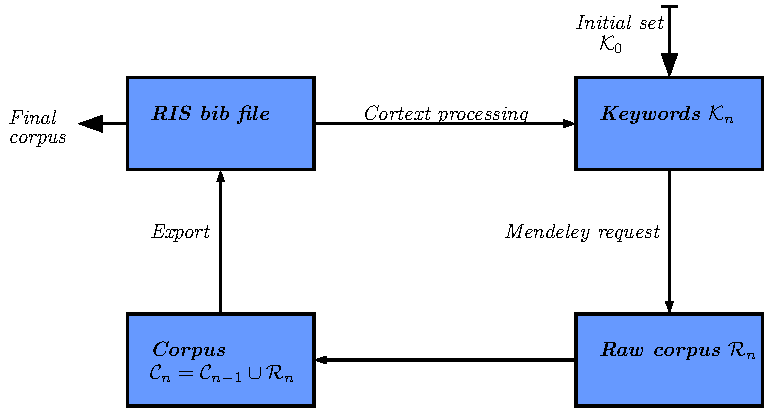
\includegraphics[width=0.8\linewidth]{Figures/QuantEpistemo/schema_algo}
\caption[Systematic review algorithm workflow][Algorithme de revue systématique]{Global workflow of the algorithm, including implementation details: catalog request is done through Mendeley API; final state of corpuses are RIS files.\label{fig:quantepistemo:algo}}{Architecture globale de l'algorithme, incluant des détails d'implémentation : la requête au catalogue est faite via l'API Mendeley \comment[FL]{tu ne l'as pas dit auparavant}; les corpus finaux sont sous forme de fichiers RIS.\label{fig:quantepistemo:algo}\comment[FL]{traduire ; pourquoi mendeley ?}}
\end{figure}
%%%%%%%%%%%%%%%%%%%%%%%%%%%%



%%%%%%%%%%%%%%%%%%%%%%%%%%%%
\paragraph{Results}{Résultats}



\bpar{
Once the algorithm is partially validated, we apply it to our question. We start from five different initial requests that were manually extracted from the various domains identified in the bibliography (that are ``city system network'', ``land use transport interaction'', ``network urban modeling'', ``population density transport'', ``transportation network urban growth''). We take the weakest assumption on parameter $N_k=100$, as it should less constrain reached domains. After having constructed corpuses, we study their lexical distances as an indicator to answer our initial question. Large distances would go in the direction of the assumption made above, i.e. that discipline self-centering may be at the origin of the lack of interest for co-evolutive models. We show in Table~\ref{tab:quantepistemo:lexical} values of relative lexical proximity, that appear to be significantly low, confirming this assumption.
}{
Les détails précis concernant l'implémentation de l'algorithme ainsi qu'une analyse de sensibilité pour vérifier la convergence sur un échantillon de requêtes initiales (typiques des champs étudiés\comment[FL]{?}) sont donnés en Appendice~\ref{app:sec:quantepistemo}. Lorsque l'algorithme a été partiellement validé par cette analyse, nous l'appliquons à notre question. Nous partons de cinq différentes requêtes initiales qui ont été manuellement extraites des divers domaines identifiés dans la bibliographie (qui sont ``city system network'', ``land use transport interaction'', ``network urban modeling'', ``population density transport'', ``transportation network urban growth'')\comment[FL]{ces mots sont nombreux, quel impact sur l'algo ?}\comment[FL]{du coup tu exclues totalement la literature francophone. pourquoi ce choix ?}\footnote{Ce choix est arbitraire,\comment[FL]{on espere que non} cette étude étant préliminaire on admet de travailler potentiellement sur des échantillons. Par exemple, l'utilisation de ``co-evolution'' n'est pas concluante car trop peu d'articles utilisent cette formulation.}. Nous prenons l'hypothèse la plus faible pour le paramètre $N_k=100$ (plus $N_k$ est grand, plus les domaines atteints devraient être moins restreints et donc plus des résultats de distance seront significatifs)\label{tab:quantepistemo:lexical}\comment[FL]{phrase non comprehensible}. Après avoir construit les corpus, nous étudions leur cohérence lexicale comme un indicateur de réponse à notre question initiale. De grande distances devraient confirmer l'hypothèse formulée ci-dessus, i.e. que des disciplines auto-centrées pourraient être à l'origine d'un manque d'intérêt pour des modèles co-évolutifs. La table~\ref{tab:quantepistemo:lexical} montre les valeurs\comment[FL]{tu n'as pas explique comment tu quantifies cela} de la proximité lexicale relative, qui est significativement basse\comment[FL]{sens ?} sachant que les chiffres peuvent directement s'interpréter comme une proportion de mots en co-occurrence, ce qui tend à confirmer notre hypothèse. Pour être plus précis tout de même, il faudrait un modèle nul\comment[FL]{?} avec des corpus aléatoires par exemple, ce qui pourrait faire l'objet de développements futurs. 
}




%%%%%%%%%%%%%%%%%%%%%%%%%%%%
\begin{table}
\caption[Stationary lexical proximities][Proximités lexicales stationnaires]{Symmetric matrix of lexical proximities between final corpuses, defined as the sum of overall final keywords co-occurrences between corpuses, normalized by number of final keywords (100). We obtain very low values, confirming that corpuses are significantly far. Size of final corpuses is given as $W$.\label{tab:quantepistemo:lexical}}{Matrice symétrique des proximités lexicales entre les corpus finaux, définies comme la somme des co-occurrences totale de mots-clés finaux entre corpus, normalisé par le nombre de mots-clés finaux (100). La taille des corpus finaux est donnée par $W$. Les valeurs obtenues pour les proximités sont considérablement faibles, ce qui confirme que les corpus sont éloignés de manière significative (voir texte).\comment[FL]{ce tableau est difficilement comprehensible ; traduire ; trop de chiffres significatifs.}\label{tab:quantepistemo:lexical}}
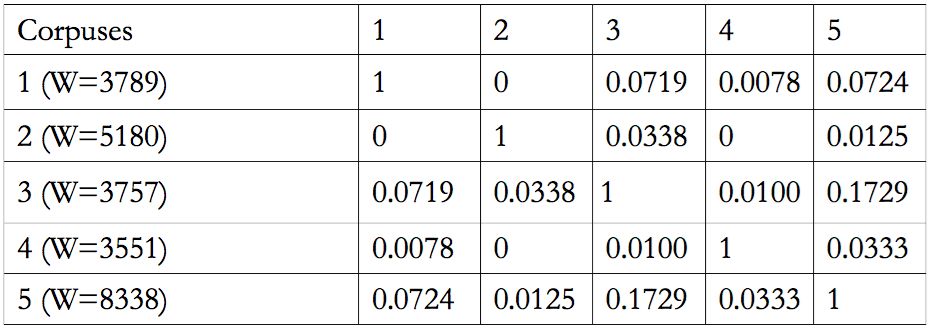
\includegraphics[width=0.8\linewidth]{Figures/QuantEpistemo/corpusesDistances}
\end{table}
%%%%%%%%%%%%%%%%%%%%%%%%%%%%




\bpar{
Possible developments can include the construction of citation networks through an automatic access to Google Scholar that provides backward citations. The confrontation of inter-cluster coefficients on the citation network for the different corpuses with lexical consistence are an essential aspect of a further validation of our results.
}{
Les développements possibles incluent la construction de réseaux de citation via un accès automatique à Google Scholar\comment[FL]{pourquoi cette plateforme et pas une autre ?} qui fournit les citations entrantes. La confrontation des coefficients inter-clusters pour le réseau de citations entre les différents corpus avec la cohérence lexicale est un aspect clé d'une validation approfondie des résultats.
}



\bpar{
The disturbing absence of models simulating the co-evolution of transportation networks and urban land-use, confirmed through a state-of-the-art covering many domain, may be due to the absence of communication between scientific disciplines studying different aspects of that problems. We have proposed an algorithmic method to give elements of answers through text-mining-based corpus extraction. First numerical results seem to confirm the assumption. However, such a quantitative analysis should not be considered alone, but rather come as a back-up for qualitative studies that will be the object of further work, such as the one lead in~\cite{commenges:tel-00923682}, in which questionnaires with historical actors of modeling provide highly relevant information.
}{
L'absence peu explicable\comment[FL]{pourquoi cette hypothese ?} a priori de modèles qui simulent la co-évolution des réseaux de transport et de l'usage du sol urbain, qui se confirme à première vue par un état de l'art couvrant des domaines disparates, pourrait être due à l'absence de communication entre les disciplines scientifiques étudiant différents aspects du problème. D'autres explications possibles qui en sont proches peuvent par exemple être le manque de cas d'application concrets de tels modèles vu les échelles temporelles mises en jeu et donc l'absence de financement propre - ce qui n'est pas si loin de l'absence d'une discipline y consacrant certains de ses objets. Cette question des portées et des échelles des modèles fera l'objet de la meta-analyse à la section suivante~\ref{sec:modelography}. Ainsi, nous ici avons proposé une méthode algorithmique pour donner des éléments de réponse par l'extraction de corpus basée sur l'analyse textuelle. Les premiers résultats numériques semblent confirmer l'hypothèse. Cependant, une telle analyse quantitative ne doit pas être considérée seule, mais devrait plutôt venir comme soutien à des études qualitatives qui peuvent être l'objet de développements futurs, comme celle menée dans~\cite{commenges:tel-00923682}, dans laquelle des questionnaires avec des acteurs historiques fournit des informations extrêmement pertinentes. \comment[FL]{ET A UNE REVUE DE BIBLIO CLASSIQUE}[(JR) faite en 2.1]
}




%--------------------------------------------------------------


%%%%%%%%%%%%%%%%%%%%%%%%
%\subsection[Indirect Bibliometrics][Bibliométrie indirecte]{Indirect bibliometrics through Complex Network analysis}{Bibliométrie Indirecte par Analyse de Réseaux Complexes}
\subsection{Indirect Bibliometrics}{Bibliométrie indirecte}

\label{subsec:indirectbibliometrics}


\bpar{
As described before, semantic analysis of final corpus does not contain all the information on disciplinary compartmentation nor on patterns of propagation of scientific knowledge as the ones contained in citation networks for example. Furthermore, data collection in the previous algorithm is subject to convergence towards self-consistent themes because of the proper structure of the method. It may give more insight about scientific social patterns of ontological choices in modeling to study communities in broader networks, that would more correspond to disciplines (or sub-disciplines depending on granularity level). We propose to reconstruct disciplines around our thematic, to obtain a more precise view of interdisciplinarity and the scientific landscape on our subject.
}{
Comme décrit précédemment, l'analyse sémantique des corpus finaux ne contient pas la totalité de l'information sur les liens entre disciplines ni sur les motifs de propagation de la connaissance scientifique comme ceux contenus dans les réseaux de citations par exemple. De plus, la collection des données dans l'algorithme précédent est sujette à convergence vers des thèmes relativement auto-cohérents de par la structure propre de la méthode. On pourrait obtenir plus d'information sur les motifs sociaux de choix ontologiques\comment[FL]{sens ?} pour la modélisation en étudiant les communautés dans des réseaux plus larges, ce qui correspondrait plus à des disciplines (ou des sous-disciplines selon le niveau de granularité). Nous proposons de reconstruire les disciplines autour de notre thématique, pour obtenir une vue plus précise de l'interdisciplinarité\comment[FL]{est ce que si les disciplines sont (re) construites par l'algo, la notion d'interdisciplinarite a le meme sens ?} et du paysage scientifique sur notre sujet. 
}


\subsubsection{Context}{Contexte}


\bpar{
Most of scientific disciplines seem to be in a need of more interdisciplinarity and transversal approaches, as highlighted by the special issue of Nature (\cite{natureInterdisc}), for diverse reasons that may include the development of vertically integrated fields conjointly with horizontal questions as detailed in the Complex Systems roadmap (\cite{2009arXiv0907.2221B}). There are naturally ongoing debates on what is exactly interdisciplinarity (many other terms such as trans-disciplinarity, cross-disciplinarity also exist) and it actually depends of involved domains : recent hybrid disciplines (see e.g. the ones underlined  by \cite{bais2010praise} such as astro-biology) are a good illustration of the case where entanglement is strong and new discoveries are vertically deep, whereas more loose fields such as ``urbanism'' which has no precise definition and integration is by essence horizontal is an other illustration of how transversal knowledge can be produced (leading to misunderstandings when recently introduced to non-aware physicists as warned by~\cite{dupuy2015sciences}). This question projects itself naturally into the field of scientific communication : what are corresponding alternatives for an efficient dissemination of knowledge ? Elements of answer to such a high-level issue imply, in an evidence-based perspective, quantitative measures of interdisciplinarity, that would be part of a multidimensional approach of the study of science that is in a way ``beyond bibliometrics'' (\cite{cronin2014beyond}).
}{
La majorité des disciplines scientifiques présentent un besoin\comment[FL]{n'y a t'il pas la deja un postulat fort ?} fort en interdisciplinarité et approches transversales, comme illustré par exemple par l'édition spéciale récente de Nature sur le sujet (\cite{natureInterdisc}), pour diverses raisons qui peuvent inclure le développement de champs intégrés verticalement\comment[FL]{sens ?} conjointement aux questions horizontales comme détaillé dans la feuille de route des Systèmes Complexes \comment[FL]{expression grandiloquente}[(JR) pas d'autre facon de nommer la roadmap](\cite{2009arXiv0907.2221B}). Les débats courants sur la nature exacte de l'interdisciplinarité sont bien sûr nombreux (d'autres termes existent comme transdisciplinarité ou cross-disciplinarité), et celle-ci dépend en fait des domaines impliqués : des disciplines hybrides apparues récemment (voir par exemples celles soulignées par \cite{bais2010praise} comme l'astro-biologie \comment[FL]{la geomatique}) sont une bonne illustration du cas où les intrications sont très fortes, tandis que des champs plus mou\comment[FL]{mauvaise strategie je pense : avant de designer une discipline en particulier, il faut preciser le sens de ``mou''} comme ``l'urbanisme'' qui n'ont pas de définition précise\comment[FL]{mal dit} montrent comment l'intégration horizontale est nécessaire et comment de la connaissance transversale peut être produite (menant à des possibles malentendus\comment[FL]{et alors ? est ce que les malentendus sont necessairement contre-productifs ?} lorsque récemment introduite trop brutalement à des physiciens comme montré par~\cite{dupuy2015sciences}). Cette question se transfère naturellement au champ de la communication scientifique : quelles sont les alternatives correspondantes pour une dissémination efficace de la connaissance ? Des éléments de réponse à une question si générale impliquent, dans une perspective \emph{evidence-based}\comment[FL]{traduire}[(JR)non traduisible - appuyer quelque part sur le sens de l'evidence-based], des mesures quantitatives de l'interdisciplinarité, qui font partie d'une approche multi-dimensionnelle de l'étude de la science, en quelque sorte ``au-delà de la bibliométrie''~\cite{cronin2014beyond}\comment[FL]{que tu n'as pas introduite}.
}


\bpar{
The possible methods for quantitative insights into epistemology are numerous. Using citation network features, a good predicting power for citation patterns is for example obtained by~\cite{2013arXiv1310.8220N}. Co-authorship networks can also be used for predictive models (\cite{2014arXiv1402.7268S}). A multilayer network approach was recently proposed in~\cite{2016arXiv160106075O}, using bipartites networks of papers and scholars, in order to produce measures of interdisciplinarity. Disciplines can be stratified into layers to reveal communities between them and therein collaboration patterns (\cite{2015arXiv150601280B}). Keyword networks are used in other fields such as economics of innovation: for example, \cite{choi2014patent} proposes a method to identify technological opportunities by detecting important keywords from the point of view of topological measures. \cite{shibata2008detecting} uses topological analysis of the citation network to detect emerging research fronts.
}{
Les méthodes potentielles pour des entrées quantitatives en épistémologie sont nombreuses. En utilisant les caractéristiques des réseaux de citation, un bon pouvoir prédictif pour les motifs de citation est par exemple obtenu par~\cite{2013arXiv1310.8220N}. Les réseaux de co-auteurs peuvent également être utilisés pour des modèles prédictifs~\cite{2014arXiv1402.7268S}. Une approche multi-couches a récemment été proposée par~\cite{2016arXiv160106075O}, utilisant des réseaux bipartites des papiers et des chercheurs, dans le but de produire des mesures d'interdisciplinarité. Les disciplines peuvent être stratifiées en couches pour révéler des communautés entre elles et ainsi des motifs de collaboration~\cite{2015arXiv150601280B}. Les réseaux de mots-clés sont utilisés dans d'autres champs comme l'économie de l'innovation : par exemple, \cite{choi2014patent} introduit une méthode pour identifier les opportunités technologiques en détectant des mots-clés importants au sens des mesures topologiques. \cite{shibata2008detecting} utilise l'analyse topologique du réseau de citations pour détecter des fronts de recherche émergents.
}

\bpar{
The approach developed here couples citation network exploration and analysis with text-mining, aiming at mapping the scientific landscape in the neighborhood of a particular corpus. The context is particularly interesting for the methodology developed. First of all, the subject studied is very broad and by essence interdisciplinary. Secondly, bibliographical data is difficult to obtain, raising the concern of how the perception of a scientific landscape may be shaped by actors of the dissemination and thus far from objective, making technical solutions as the ones consequently developed here crucial tools for an open and neutral science. Our approach combine semantic communities analysis (as done in~\cite{2016arXiv160208451P} for papers in physics but with keyword extraction ; \cite{2015arXiv151003797G} analyses semantic networks of political debates) with citation network to extract e.g. interdisciplinarity measures. Our contribution differs from the previous works quantifying interdisciplinarity as it does not assume predefined domains nor classification of the considered papers, but reconstructs from the bottom-up the fields with the endogenous semantic information. \cite{nichols2014topic} already introduced a close approach, using Latent Dirichlet Allocation topic modeling to characterize interdisciplinarity of awards in particular sciences. \cite{lariviere201410} quantifies interdisciplinarity over a long time range by looking at the field of references of publications.
}{
L'approche développée ici couple exploration et analyse de réseau de citation avec analyse textuelle, dans le but de cartographier le paysage scientifique dans le voisinage d'un corpus donné. Le contexte est particulièrement intéressant pour la méthodologie développée. Premièrement, le sujet étudié est très large et par essence interdisciplinaire. Deuxièmement, les données bibliographiques sont difficiles à obtenir, soulevant la question de comment la perception d'un horizon scientifique peut être déterminée par les acteurs de la dissémination et donc loin d'être objective, rendant les solutions techniques comme celle développée ici en conséquence des outils cruciaux pour une science ouverte et neutre. Notre approche combine une analyse des communautés sémantiques (comme fait dans~\cite{2016arXiv160208451P} pour les articles en physique mais sans extraction des mots-clés, ou par \cite{2015arXiv151003797G} pour un analyse des réseaux sémantiques de débats politiques) avec celle du réseau de citations pour extraire par exemple des mesures d'interdisciplinarité. Notre contribution se démarque des travaux précédents quantifiant l'interdisciplinarité puisqu'elle ne suppose pas de domaines a priori ou une classification des références considérées, mais reconstruit par le bas les champs via l'information sémantique endogène. \cite{nichols2014topic} introduit une approche similaire, utilisant le modèle d'extraction de thématiques \emph{Latent Dirichlet Allocation} pour caractériser l'interdisciplinarité de récompenses dans des sciences précises. \cite{lariviere201410} quantifie l'interdisciplinarité sur une longue période temporelle en étudiant l'étendue de la bibliographie des publications.\comment[FL]{vague}
}



%%%%%%%%%%%%%%%%%%%%%%%
\subsubsection{Database Construction}{Données}


\bpar{
Our approach imposes some requirements on the dataset used, namely: (i) cover a certain neighborhood of the studied journal in the citation network in order to have a consistent view on the scientific landscape; (ii) have at least a textual description for each node. For these to be met, we need to gather and compile data from heterogeneous sources, using therefore a specific application, which general architecture is synthesized in Fig.~\ref{fig:datacollection}. For the sake of simplicity, we will denote by \emph{reference} any standard scientific production that can be cited by another (journal paper, book, book chapter, conference paper, communication, etc.) and contains basic records (title, abstract, authors, publication year). We will work in the following on networks of references. Note that one significant contribution of this paper is the construction of such an hybrid dataset from heterogeneous sources, and the development of associated tools that can be reused and further developed for similar purposes.
}{
Notre approche implique des spécifications pour le jeu de données utilisé, à savoir : (i) couvrir un voisinage conséquent du corpus étudié dans le réseau de citation afin d'avoir une vue la moins biaisée possible du paysage scientifique ; (ii) avoir au moins une description textuelle pour chaque noeud.\comment[FL]{B} Pour cela, nous rassemblons et compilons les données de sources hétérogènes en utilisant une architecture et implémentation spécifiques, décrites en Appendice~\ref{app:sec:cybergeo}. Pour simplifier, nous dénommons \emph{référence} toute production scientifique standard\footnote{ce qui est bien sûr sujet à débat, voir nos discussion en ouverture sur l'évolution des modes de communication scientifique} qui peut être citée par une autre (articles de journaux, livre, chapitre de livre, article d'actes, communication, etc.) et contient des informations de base (titre, résumé, auteurs, année de publication). Nous travaillons par la suite sur le réseau des références. Il est important de noter qu'une contribution fondamentale\comment[FL]{le dire avant} de cette partie consiste en la construction de jeux de données hybrides à partir de sources hétérogènes, et les développement des outils associés qui peuvent être réutilisés et améliorés pour des applications similaires.
}

\paragraph{Initial Corpus}{Corpus Initial}

Notre corpus initial est construit à partir de l'état de l'art établi en~\ref{sec:modelingsa}. Sa composition complète est donnée en Appendice~\ref{app:sec:quantepistemo}. Celui-ci est pris de taille raisonnable\comment[FL]{sens ?}, mais les méthodes utilisées ici ont été développées sur des données massives, pour les brevets par exemple~\cite{bergeaud2017classifying}.


\paragraph{Citation Data}{Données de citation}

\bpar{
Citation data is collected from \texttt{Google Scholar}\comment[FL]{police}, that is the only source for incoming citations~\cite{noruzi2005google} in our case as the journal is poorly in other databases\footnote{or was just added as in the case of \textit{Web of Science}, indexing \textit{Cybergeo} since May 2016}. We are aware of the possible biaises using this single source (see e.g.~\cite{bohannon2014scientific})\footnote{or \texttt{http:\/\/iscpif.fr\/blog\/2016\/02\/the-strange-arithmetic-of-google-scholars}}, but these critics are more directed towards search results than citation counts. %The automatic collection requires the use of an open source data crawling software to pipe requests, namely \texttt{TorPool}~\cite{torpool} that provides a Java API allowing an easy integration into our application. Using it, a crawler can retrieve html pages and get backward citation data, i.e. all citing articles for a given initial article.
 We retrieve that way two sub-corpuses: references \emph{citing} Cybergeo and references \emph{citing the ones cited} by cybergeo. At this stage, the full corpus contains around $4\cdot10^5$ references.
}{
Le réseau de citations est reconstruit à partir de \texttt{Google Scholar} qui est souvent l'unique source des citations entrantes~\cite{noruzi2005google} puisqu'en science humaines les ouvrages ne sont pas systématiquement référencés par les bases fournissant des services (payants) comme le réseau de citation.\footnote{Par exemple, le journal Cybergeo n'est indexé dans le \emph{Web of Science} que depuis mai 2016, suite à des négociations ardues et non sans contrepartie.} Nous sommes conscients des biais possibles de l'utilisation de cette source unique (voir par exemple~\cite{bohannon2014scientific})\footnote{ou \texttt{http:\/\/iscpif.fr\/blog\/2016\/02\/the-strange-arithmetic-of-google-scholars}}, mais ces critiques sont plutôt dirigées vers les résultats de recherche plutôt que les comptes de citations. Nous récoltons ainsi les références \emph{citantes} à profondeur deux, c'est à dire les références citant le corpus initial et celles citant celles-ci. Le réseau obtenu contient $V=9462$ références correspondant à $E=12004$ liens de citation. Concernant les langues, l'anglais représente 87\% du corpus, le français 6\%, l'espagnol 3\%, l'allemand 1\%, complété par des langues comme le mandarin pouvant être indéfinies (la détection de celui-ci étant peu fiable). Le corpus n'est pas très international (contrairement par exemple au thème de la croissance urbaine, étudié pour le développement thématique sur les liens entre économie et géographie développé en~\ref{app:sec:ecogeo}).
}

\paragraph{Text Data}{Données textuelles}

\bpar{
A textual description for all references is necessary for a complete semantic analysis. We use for this an other source of data, that is the online catalog of \textit{Mendeley} reference manager software~\cite{mendeley}. It provides a free API allowing to get various records under a structured format. Although not complete, the catalog provides a reasonable coverage (over 55\%), yielding a final corpus with full abstracts of size $2.1\cdot 10^5$, which structure is recalled in Fig.~\ref{fig:citationnetwork}
}{
Pour mener l'analyse sémantique, une description suffisamment conséquente est nécessaire. Nous collectons pour cela les résumés pour le réseau précédent. Ceux-ci sont disponibles pour environ un tiers des références, donnant $V=3510$ noeuds avec description textuelle.
}



%%%%%%%%%%%%%%%%%%
\subsubsection{Results}{Résultats}


\paragraph{Citation Network Properties}{Réseau de citations}


Des statistiques basiques pour le réseau de citation donnent déjà des informations intéressantes. Le réseau a un degré moyen de $\bar{d}=2.53$ et une densité de $\gamma=0.0013$. Le degré entrant moyen (qui peut être interprété comme un facteur d'impact stationnaire) est de 1.26, ce qui est relativement élevé pour des sciences humaines. Il est important de noter sa connexité faible, ce qui signifie que les domaines initiaux ne sont pas en isolation totale : les références initiales sont partagées à un degré minimal par les différents domaines. Nous travaillons sur la suite sur le sous-réseau des noeuds comprenant au moins deux liens, pour extraire le coeur de la structure du réseau et se débarrasser de l'effet ``grappe''. De plus, le réseau est nécessairement complet entre ces noeuds puisqu'on est remonté au deuxième niveau. Nous procédons à une détection de communautés par l'algorithme de Louvain, sur le réseau non-dirigé correspondant. On obtient 13 communautés\comment[FL]{comment ? c'est elliptique}[(JR) dit juste avant, algo de Louvain], de modularité dirigée 0.66, extrêmement significative en comparaison à une estimation par bootstrap de la même mesure sur le graphe aléatoirement rebranché qui donne une modularité de $0.0005 \pm 0.0051$ sur $N=100$ répétitions. Les communautés font sens de manière thématique, puisqu'on retrouve pour les plus grosses les domaines suivants : LUTI (18\% du réseau), Géographie Urbaine et des Transports (16\%), Planification des infrastructures (12\%), Planification intégrée - TOD (6\%), Réseaux Spatiaux (17\%), Etudes d'accessibilité (18\%).\comment[FL]{quelle est leur coherence interne ? comment as tu donne les noms ?}[(JR) cf remarque de Caruso a ECTQG] La Fig.~\ref{fig:quantepistemo:citnw} permet de visualiser les relations de ces domaines. Il est intéressant d'observer que les travaux des économistes et des physiciens dans le domaine tombent dans la même catégorie d'étude des \emph{Spatial Networks}. En effet, la littérature citée par les physiciens comporte souvent plus d'ouvrage en économie qu'en géographie, tandis que les économistes utilisent des techniques d'analyse de réseau. Ensuite, le planning, l'accessibilité, les LUTI et le TOD sont très proches mais se distinguent dans leur spécificités: le fait qu'ils apparaissent dans des communautés séparées est un résultat en lui-même témoignant d'une certaine séparation.\comment[FL]{phrase alambiquee} Ceux-ci font le pont entre les approches Réseaux spatiaux et les approches géographiques, qui comportent une partie importante de sciences politiques par exemple. Les liens entre physique et géographie restent très faibles. Ce panorama dépend bien sûr du corpus initial, mais nous permet de mieux comprendre le contexte de celui-ci dans son environnement disciplinaire.


%%%%%%%%%%%%%%%%%
\begin{figure}[!ht]
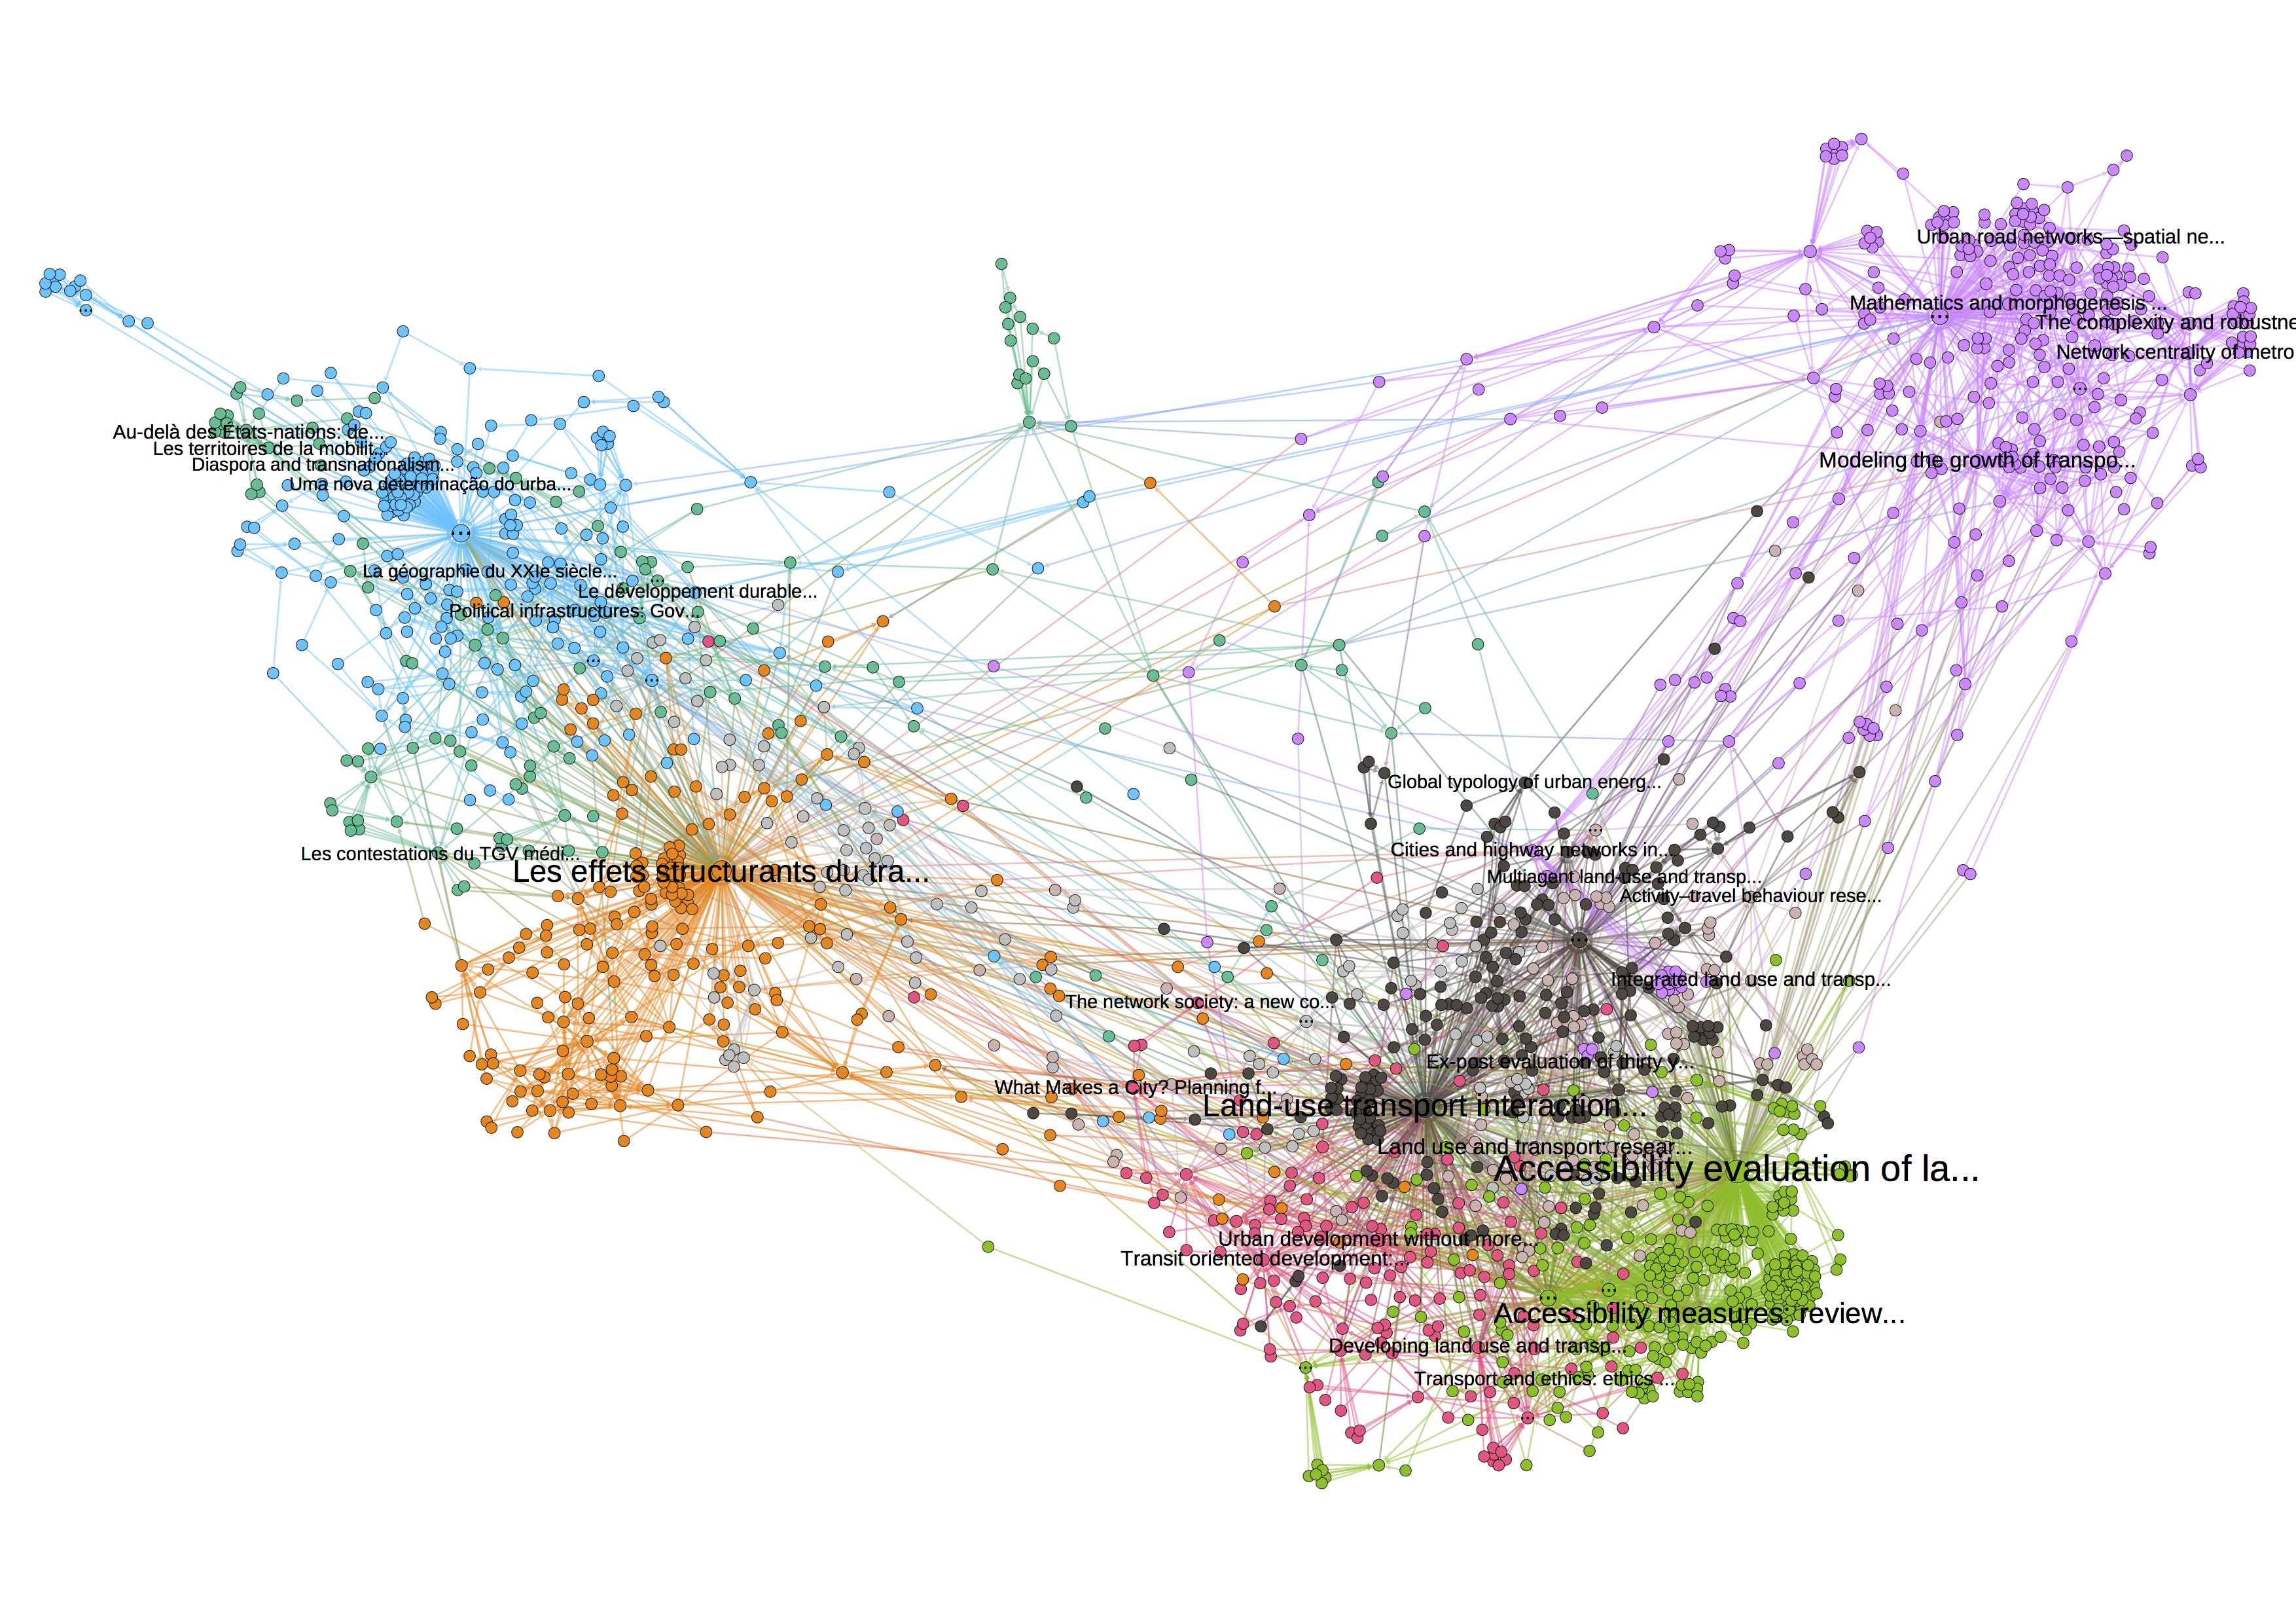
\includegraphics[width=\linewidth]{Figures/QuantEpistemo/rawcore}
\caption[Citation Network][Réseau de citations]{\textbf{Citation Network}\label{fig:quantepistemo:citnw}}{\textbf{Réseau de citations.} Nous visualisons les références ayant au moins deux liens, par un algorithme de force-atlas. Les couleurs donnent les communautés décrites dans le texte. En orange, bleu, turquoise: géographie urbaine, géographie des transports, sciences politiques ; en rose, noir, vert: planning, accessibilité, LUTI ; en violet : réseaux spatiaux (physique et économie).\label{fig:quantepistemo:citnw}}
\end{figure}
%%%%%%%%%%%%%%%%%





%%%%%%%%%%%%%%%%%%
\paragraph{Semantic Communities}{Communautés Sémantiques}


L'extraction des mots-clés est faite suivant une heuristique inspirée de~\cite{chavalarias2013phylomemetic}. La description complète de la méthode et de son implémentation est donnée en Appendice~\ref{app:sec:cybergeo}. Elle se base sur les relations au second ordre entre les entités sémantiques, qui sont des \emph{n-grams}, c'est à dire des mots-clés multiples pouvant avoir une longueur jusqu'à 3. Celles-ci sont estimées via la matrice de co-occurrence, dont les propriétés statistiques fournissent une mesure de déviation à des co-occurrences uniformes, qui est utilisée pour juger la pertinence des mots-clés. Sélectionnant un nombre fixe de mots-clés pertinents $K_W = 10000$, nous pouvons ensuite construire un réseau pondéré par les co-occurrences.


\bpar{
The topology of raw networks does not allow the extraction of clear communities, in particular because of the presence of hubs that correspond to frequent terms common to many fields (e.g. \texttt{model}, \texttt{space}). We assume these highest degree terms do not carry specific information on particular classes and can be thus filtered given a maximal degree threshold $k_{max}$. Similarly, edge with small weight are considered as noise and filtered according to a minimal edge weight threshold $\theta_w$. Keywords are preliminary filtered by a document frequency window $\left[ f_{min},f_{max} \right]$ which is slightly different from network filtering and complementary. A sensitivity analysis of resulting network topology to these parameters is presented in Fig.~\ref{fig:sensitivity}. We choose parameter values that maximize modularity under the constraint of a community number and size distribution of same magnitude as technological classes. This multi-objective optimization does not have a unique solution as objectives are somehow contradictory, and a compromise point must be chosen.
}{
La topologie du réseau brut ne permet pas l'extraction claire de communautés, en particulier à cause de hubs qui correspondent à des termes fréquents commun à de nombreux champs (e.g. \texttt{model}, \texttt{space})\comment[FL]{statut de ces mots ?}. Nous faisons l'hypothèse que ces termes à fort degré ne portent pas d'information particulière sur des classes données et peuvent ainsi être filtrés étant donné un seuil de degré maximal $k_{max}$ (on s'intéresse alors à ce qui fait la spécificité de chaque domaine). De la même manière, les liens avec un poids faibles sont considérés comme du bruit et filtrés selon un seuil de poids minimal $\theta_w$. La méthode générique permet de plus une filtration préliminaire des mot-clés, complémentaire à la filtration topologique, par fréquence d'apparition dans les documents $\left[ f_{min},f_{max} \right]$, à laquelle les résultats ne sont pas sensibles dans notre cas. L'analyse de sensibilité des caractéristiques du réseau filtré, notamment de sa taille, modularité et structure des communautés, est donnée en~\ref{app:sec:quantepistemo}. Nous choisissons des valeurs de paramètres permettant une optimisation multi-objectif entre modularité et taille du réseau, $\theta_w = 10,k_{max} = 500$, par le choix d'un point compromis sur un front de Pareto, qui donne un réseau sémantique de taille $(V=7063,E=48952)$. Celui-ci est visualisé en Appendice~\ref{app:sec:quantepistemo}.
}


\bpar{
We then retrieve communities in the semantic network (using standard Louvain algorithm, with the optimized filtering parameters). communities correspond to well-defined scientific fields (and/or domains, approaches). An expert validation allow us to give names to these, a more complicated naming procedure would eventually be possible (as in~\cite{yang2000improving} for the case of patents 
 where a chi-square test on distribution of documents in classes), but we prefer to stick here to a certain level of supervision. Table~\ref{tab:domains} summarizes the communities 
}{
Nous récupérons ensuite les communautés dans le réseau par un clustering de Louvain standard sur le réseau filtré optimal. On obtient 20 communautés pour une modularité de 0.58. Celles-ci sont examinées à la main pour être nommées, les techniques de désignation automatique~\cite{yang2000improving} n'étant pas assez élaborées et ne font pas la distinction implicite entre champs thématiques et méthodologiques par exemple (en fait entre les domaines de connaissance, voir~\ref{sec:knowledgeframework}) qui est une dimension supplémentaire que nous ne traitons pas ici, mais nécessaire pour avoir des désignations parlantes. Les communautés sont décrites en Table~\ref{tab:quantepistemo:semanticdomains}. On voit tout de suite la complémentarité avec l'approche par citation, puisque se dégagent ici à la fois des sujet d'étude (High Speed Rail, Maritime Networks), des domaines et méthodes (Networks, Remote Sensing, Mobility Data Mining), des domaines thématiques (Policy), des méthodes pures (Agent-based Modeling, Measuring). Ainsi, une référence peut mobiliser plusieurs de ces communautés. On a de plus une granularité plus fine de l'information. L'effet du langage est puissant puisque la géographie française se distingue en une catégorie séparée (des analyses poussées pourraient être envisagées pour mieux comprendre le phénomène et en tirer parti: sous-communautés, reconstruction d'un réseau spécifique, études par traduction ; mais celles-ci sont hors de propos dans cette étude exploratoire). On constante l'importance des réseaux, des problématiques de sciences politiques et socio-économiques. Nous mobiliserons la première catégorie dans la plupart des modèles développés, mais en gardant en tête l'importance des problématiques liées à la gouvernance, nous réaliserons un travail spécifique en~\ref{sec:lutetia}.
}




%%%%%%%%%%%%%%%%%%
\begin{table}
\caption[Semantic communities][Communautés sémantiques]{Disciplines/domains/fields reconstructed from community detection in the semantic network}{\textbf{Description des communautés sémantiques.} On donne leur taille, leur proportion en quantité de mots-clés cumulés sur l'ensemble du corpus, et des mots-clés représentatifs sélectionnés par degré maximal.\comment[FL]{pourquoi ces mots sont ils tronques ?}[(JR) cest explique dans le texte (surtout en annexe) il s'agit de stem]}
\label{tab:quantepistemo:semanticdomains}
\begin{tabular}{llll}
\hline\noalign{\smallskip}
Name & Size & Weight & Keywords  \\
\noalign{\smallskip}\hline\noalign{\smallskip}
Networks & 820 & 13.57\% & \texttt{social network, spatial network, resili} \\
Policy & 700 & 11.8\% & \texttt{actor, decision-mak, societi} \\
Socio-economic & 793 & 11.6\% & \texttt{neighborhood, incom, live} \\
High Speed Rail & 476 & 7.14\% & \texttt{high-spe, corridor, hsr} \\
French Geography & 210 & 6.08\% & \texttt{système, développement, territoire} \\
Education & 374 & 5.43\% & \texttt{school, student, collabor} \\
Climate Change & 411 & 5.42\% & \texttt{mitig, carbon, consumpt} \\
Remote Sensing & 405 & 4.65\% & \texttt{classif, detect, cover} \\
Sustainable Transport & 370 & 4.38\% & \texttt{sustain urban, travel demand, activity-bas} \\
Traffic & 368 & 4.23\% & \texttt{traffic congest, cbd, capit} \\
Maritime Networks & 402 & 4.2\% & \texttt{govern model, seaport, port author} \\
Environment & 289 & 3.79\% & \texttt{ecosystem servic, regul, settlement} \\
Accessibility & 260 & 3.23\% & \texttt{access measur, transport access, urban growth} \\
Agent-based Modeling & 192 & 3.18\% & \texttt{agent-bas, spread, heterogen} \\
Transportation planning & 192 & 3.18\% & \texttt{transport project, option, cba} \\
Mobility Data Mining & 168 & 2.49\% & \texttt{human mobil, movement, mobil phone} \\
Health Geography & 196 & 2.49\% & \texttt{healthcar, inequ, exclus} \\
Freight and Logistics & 239 & 2.06\% & \texttt{freight transport, citi logist, modal} \\
Spanish Geography & 106 & 1.26\% & \texttt{movilidad urbana, criteria, para} \\
Measuring & 166 & 1.0\% & \texttt{score, sampl, metric} \\
\noalign{\smallskip}\hline
\end{tabular}
\end{table}
%%%%%%%%%%%%%%%%%%



%%%%%%%%%%%%%%%%%%
\paragraph{Measures of Interdisciplinarity}{Mesures d'interdisciplinarité}


\bpar{
Distribution of keywords within communities provides an article-level interdisciplinarity.
Combination of citation and semantic layers in the hyper-network provide second order interdisciplinarity measures, that we don't use here because of the modest size of the citation network. More precisely, a reference can be viewed as a probability vector on semantic classes.
}{
La distribution des mots clés dans les communautés permettent de définir une mesure d'interdisciplinarité au niveau de l'article. La combinaison des couches de citation et sémantique dans l'hyperréseau fournit des mesures d'interdisciplinarité au second ordre (motifs sémantiques des cités ou des citants), que nous n'utiliserons pas ici à cause de la taille modeste du réseau de citation (voir \ref{app:sec:cybergeo} et \ref{app:sec:patents}). Plus précisément, une référence $i$ peut être vue comme un vecteur de probabilités sur les classes sémantiques $j$, qu'on notera sous forme matricielle $\mathbf{P}=(p_{ij})$. Celles-ci sont estimées simplement par les proportions de mots-clés classifiés dans chaque classe pour la référence. Une mesure classique d'interdisciplinarité~\cite{bergeaud2017classifying} est alors $I_i = 1 - \sum_j p_{ij}^2$. Soit $\mathbf{A}$ la matrice d'adjacence du réseau de citation, et soit $\mathbf{I}_k$ les matrices de selection des lignes correspondants à la classe $k$ de la classification de citation: $Id\cdot \mathbbm{1}_{c(i)=k}$, telle que $I_k \cdot A \cdot I_{k'}$ donne exactement les citations de $k$ vers $k'$. La proximité de citation entre les communautés de citation est alors définie par $c_{kk'} = \sum \mathbf{I}_k \cdot \mathbf{A} \cdot \mathbf{I}_{k'} /  \sum \mathbf{I}_k \cdot \mathbf{A}$. On définit la proximité sémantique en définissant une matrice de distance entre références par $\mathbf{D} = d_{ii'}=\sqrt{\frac{1}{2}\sum (p_{ij}-p{i'j})^2}$ puis la proximité sémantique par $s_{kk'} = \mathbf{I}_k \cdot \mathbf{D} \cdot \mathbf{I}_{k'} / \sum \mathbf{I}_k \sum \mathbf{I}_{k'}$. Nous montrons en Fig.~\ref{fig:quantepistemo:interdisc} les valeurs de ces différentes mesures, ainsi que la composition sémantique des communautés de citation, pour les classes sémantiques majoritaires. La distribution de $I_i$ montre que les papiers gravitant dans le domaine du LUTI sont les plus interdisciplinaires dans les termes utilisés, ce qui pourrait être lié à leur caractère appliqué. Les autres disciplines sont dans des motifs similaires, à part la géographie et la planification des infrastructures qui présentent des distributions quasi-uniformes, témoignant de l'existence de références très spécialisées dans ces classes. Ce n'est pas nécessairement étonnant vu les sous-champs pointus exhibés (sciences politiques par exemples, et de même les études prospectives type coût-bénéfices sont très étriquées). Ce premier croisement des couches nous confirme les spécificités de chaque champ. Concernant les compositions sémantiques, la plupart agissent comme validation externe vu les classes majoritaires. Le champ le moins concerné par les problème socio-économiques est la planification des infrastructure, ce qui donnera du grain à moudre aux détracteurs de la technocratie. Les questions de changement climatique et durabilité sont relativement bien répartie. Enfin, les ouvrages géographiques concernent en majorité des problèmes de gouvernance. Les matrices de proximité confirment la conclusion de la sous-section précédente en terme de citation, les partages étant très faibles, les plus hautes valeurs étant jusqu'à un quart de la planification vers la géographie et des LUTI vers le TOD (mais pas l'inverse, les relations peuvent être à sens unique). Hors, les proximités sémantiques montrent par exemple que LUTI, TOD, Accessibility et Networks sont proches dans leur termes, ce qui est logique pour les trois premiers, et confirme pour le dernier que les physiciens se basent majoritairement sur les méthodes des ces champs liés au planing pour légitimer leur travaux. La géographie est totalement isolée, sa plus proche voisine étant la planification des infrastructures. Cette étude est très utile pour notre propos, puisqu'elle montre des domaines cloisonnés partageant des termes at donc a priori des problématiques et sujet commun. On ne se parle pas alors qu'on parle des languages pas si lointains, d'où la pertinence accrue de les faire parler d'une commune voie dans nos travaux : nos modèles devront mobiliser des éléments, ontologies et échelles de ces différents champs.
}



%%%%%%%%%%%%%%%%%%
\begin{figure}
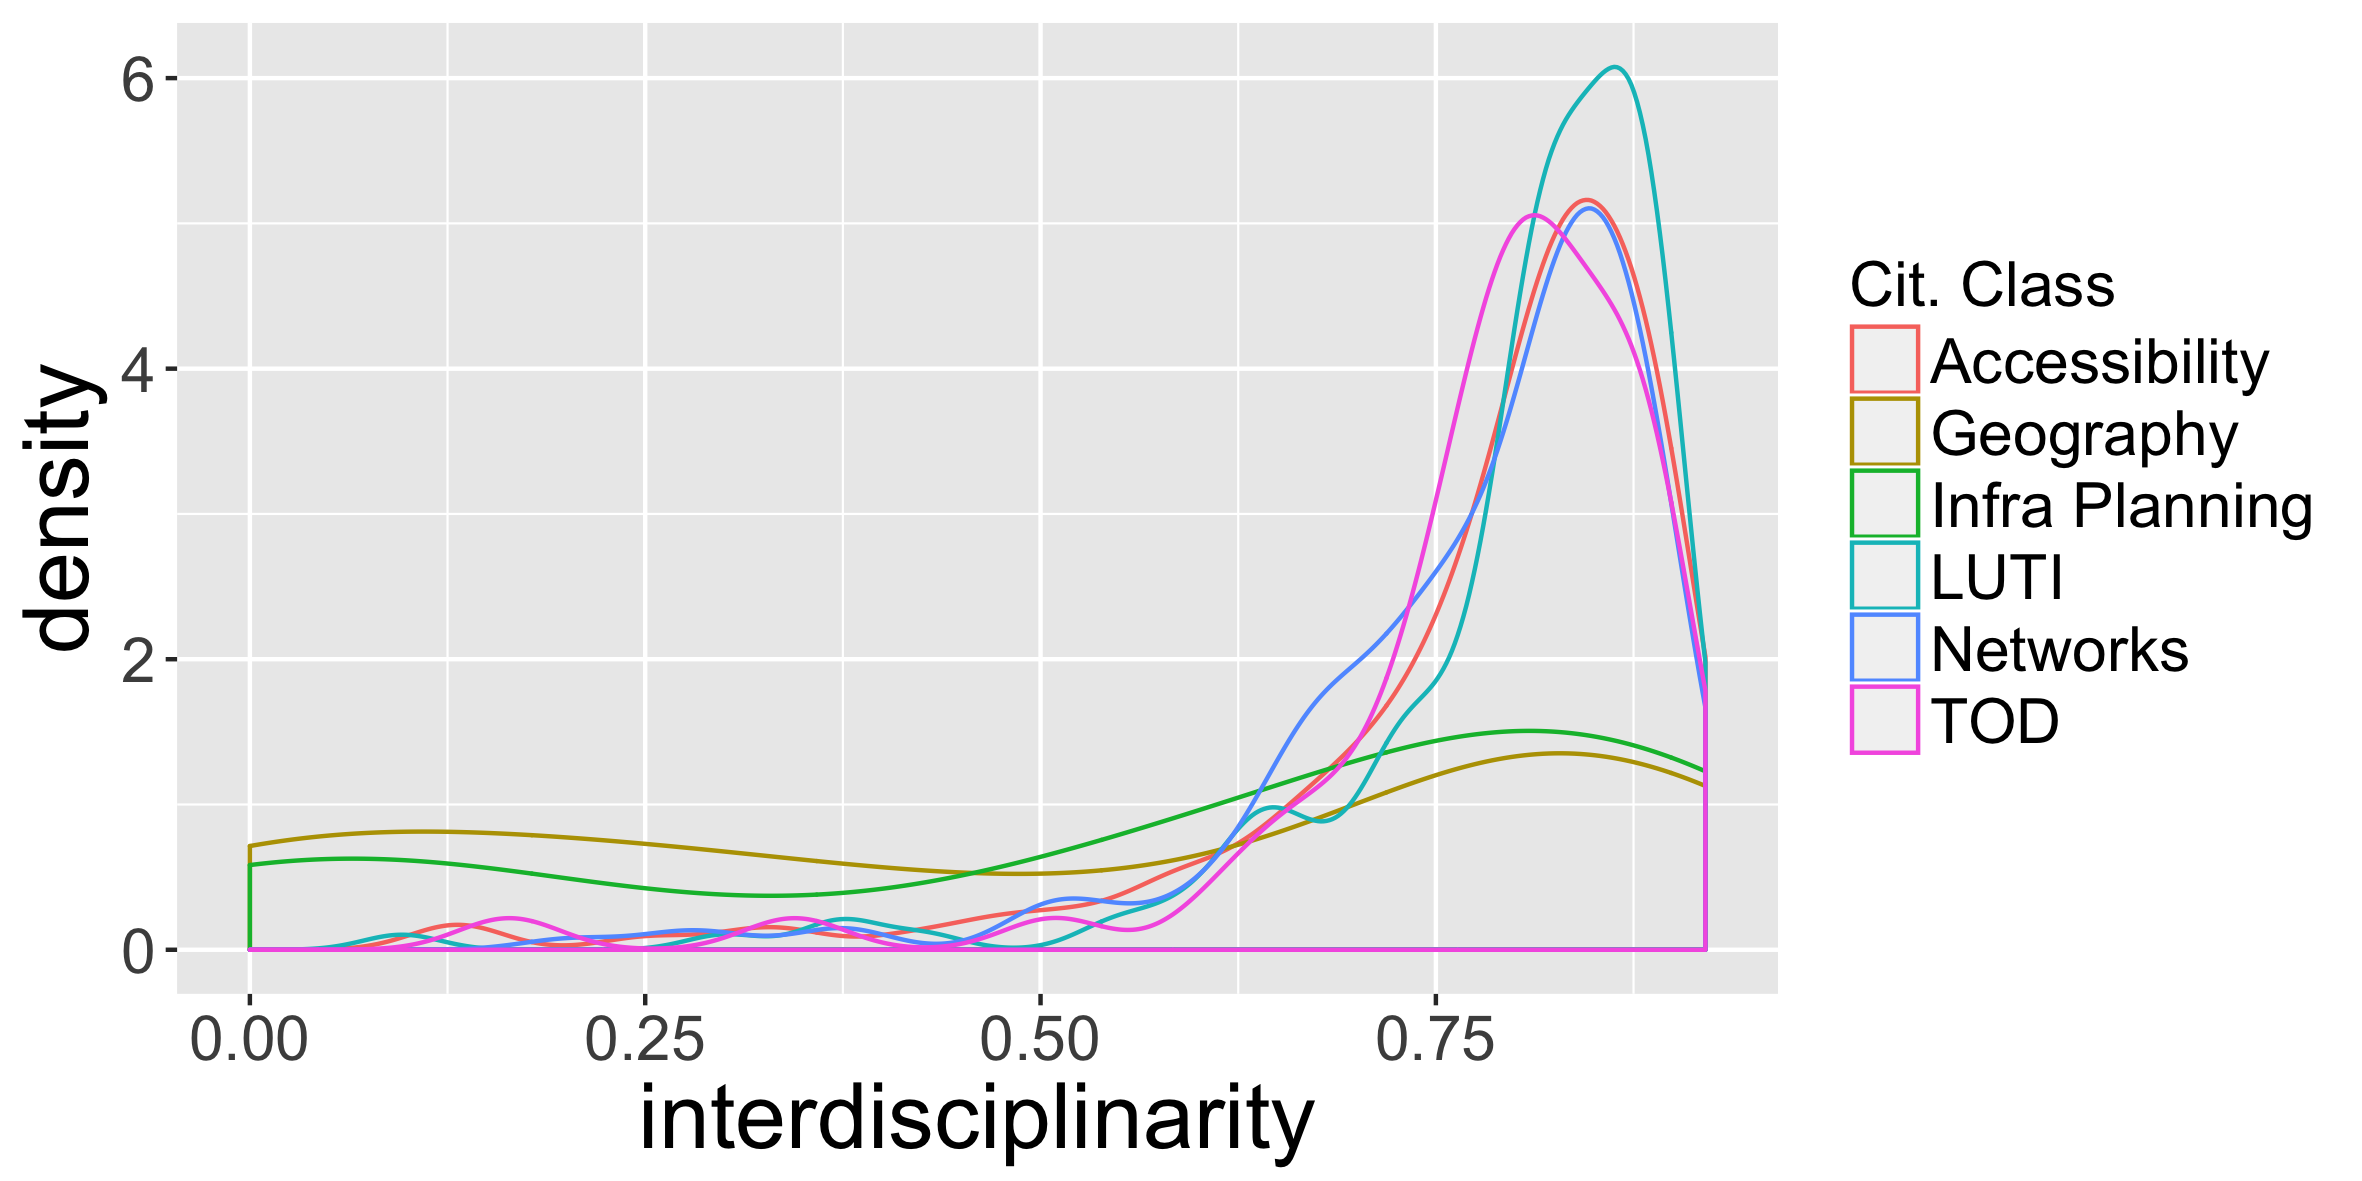
\includegraphics[width=0.49\linewidth]{Figures/QuantEpistemo/interdisciplinarities}
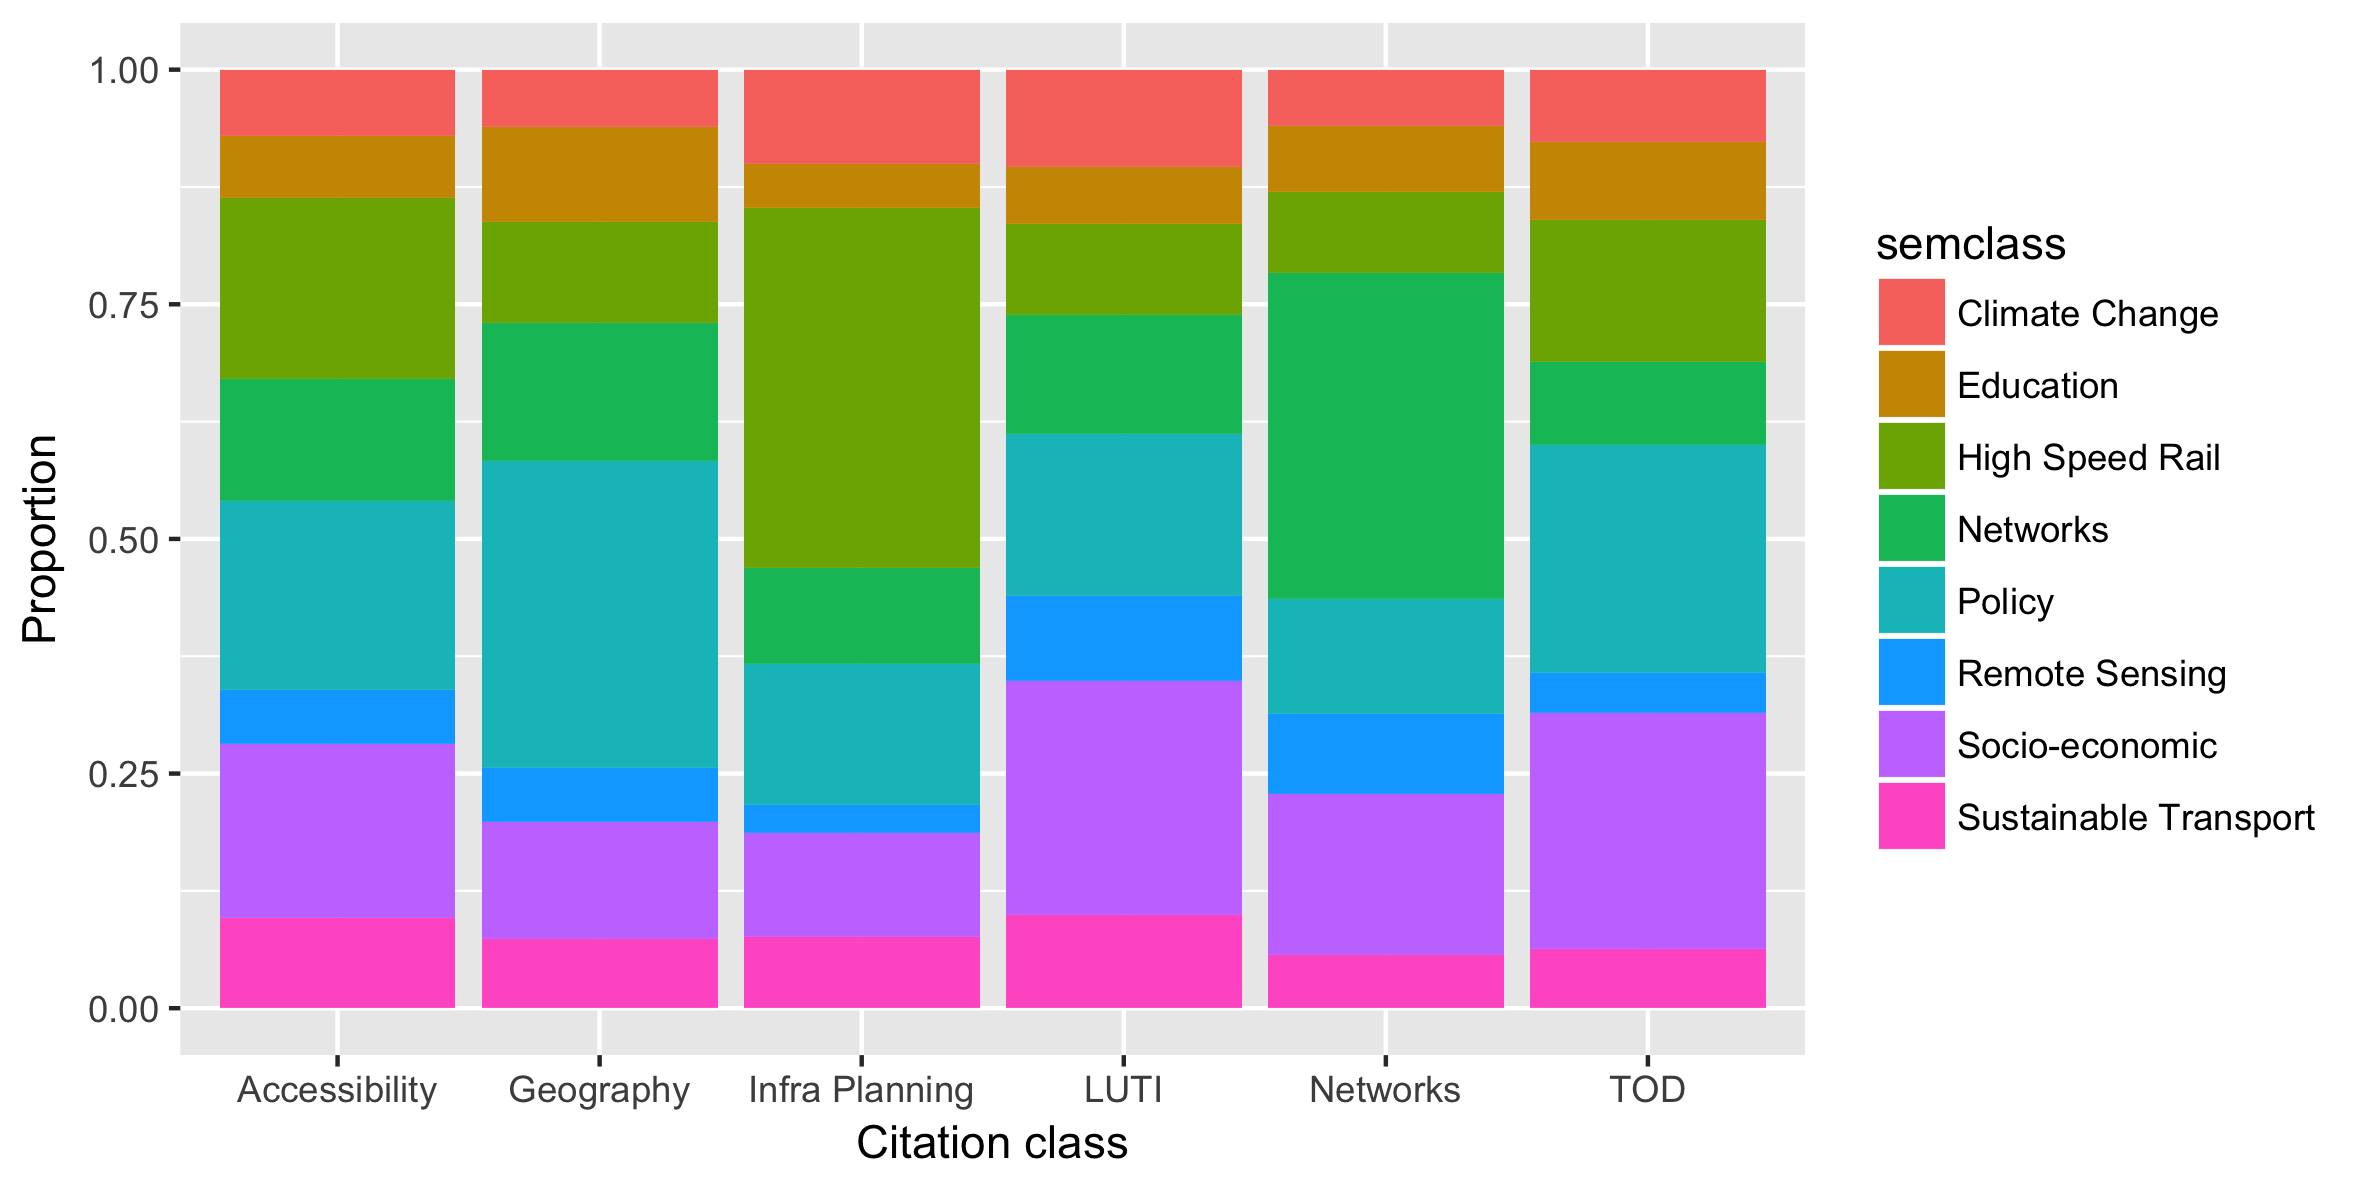
\includegraphics[width=0.49\linewidth]{Figures/QuantEpistemo/compo_proportion}\\
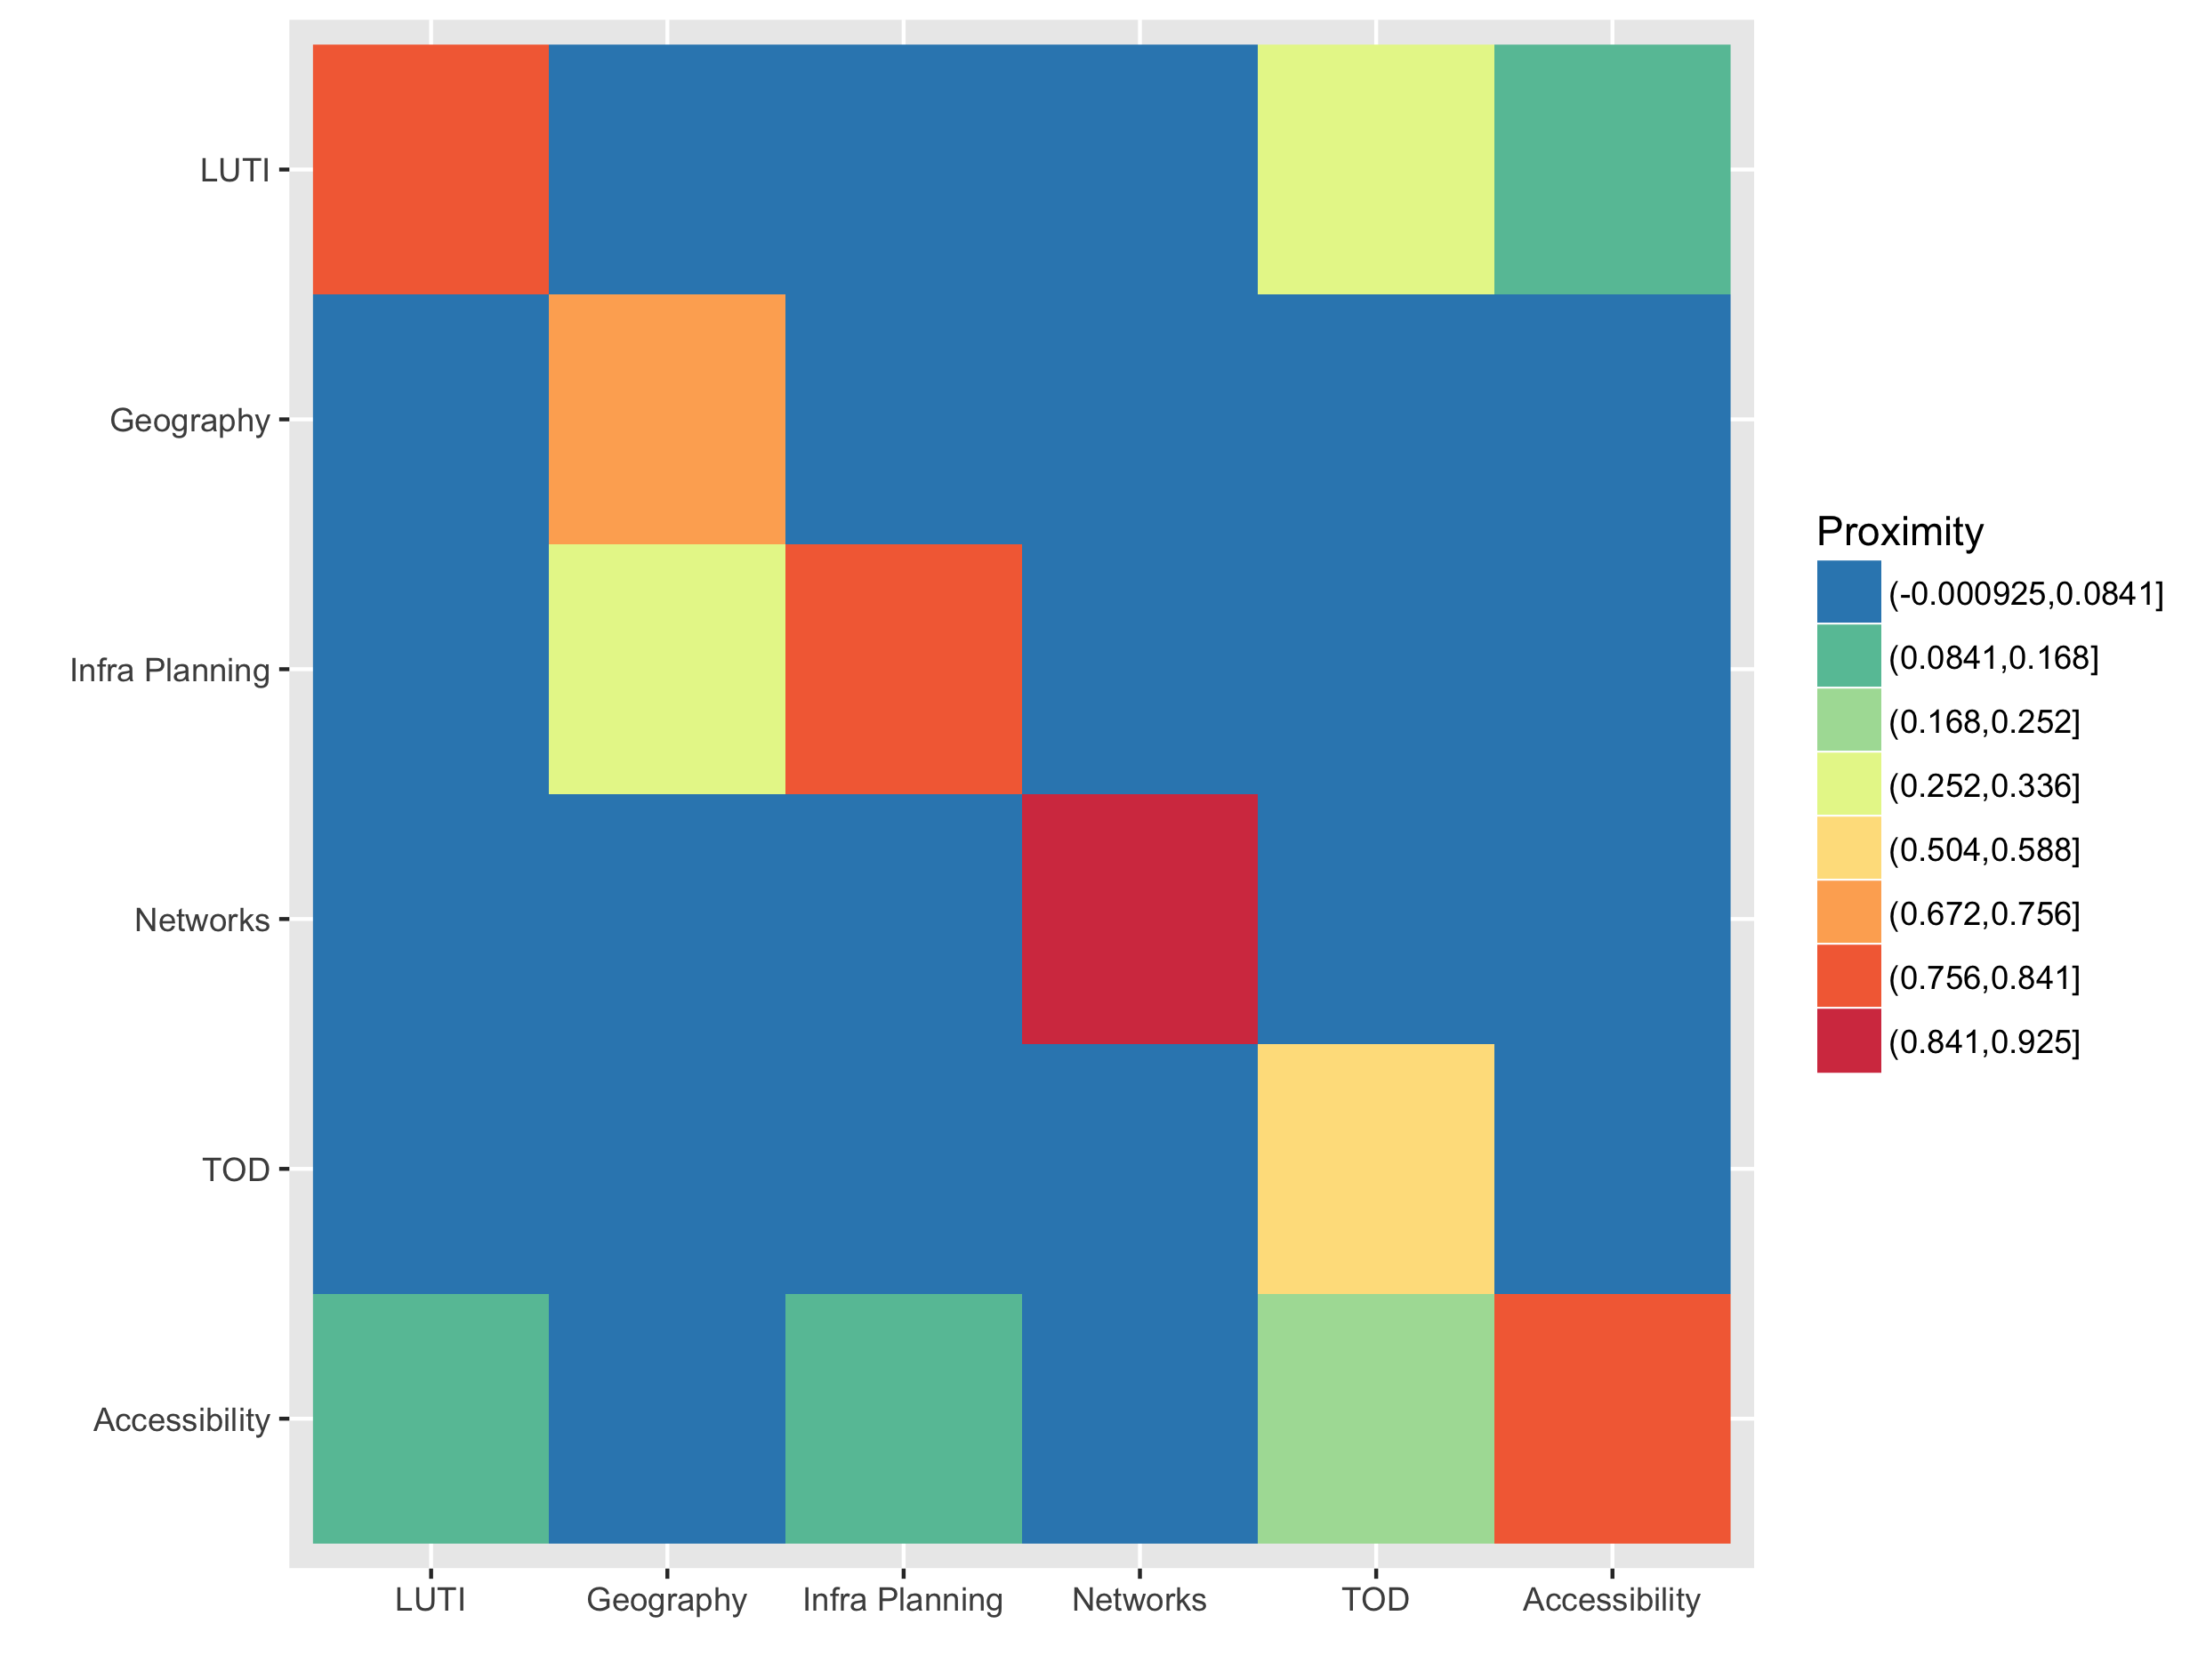
\includegraphics[width=0.49\linewidth]{Figures/QuantEpistemo/citation_proximities}
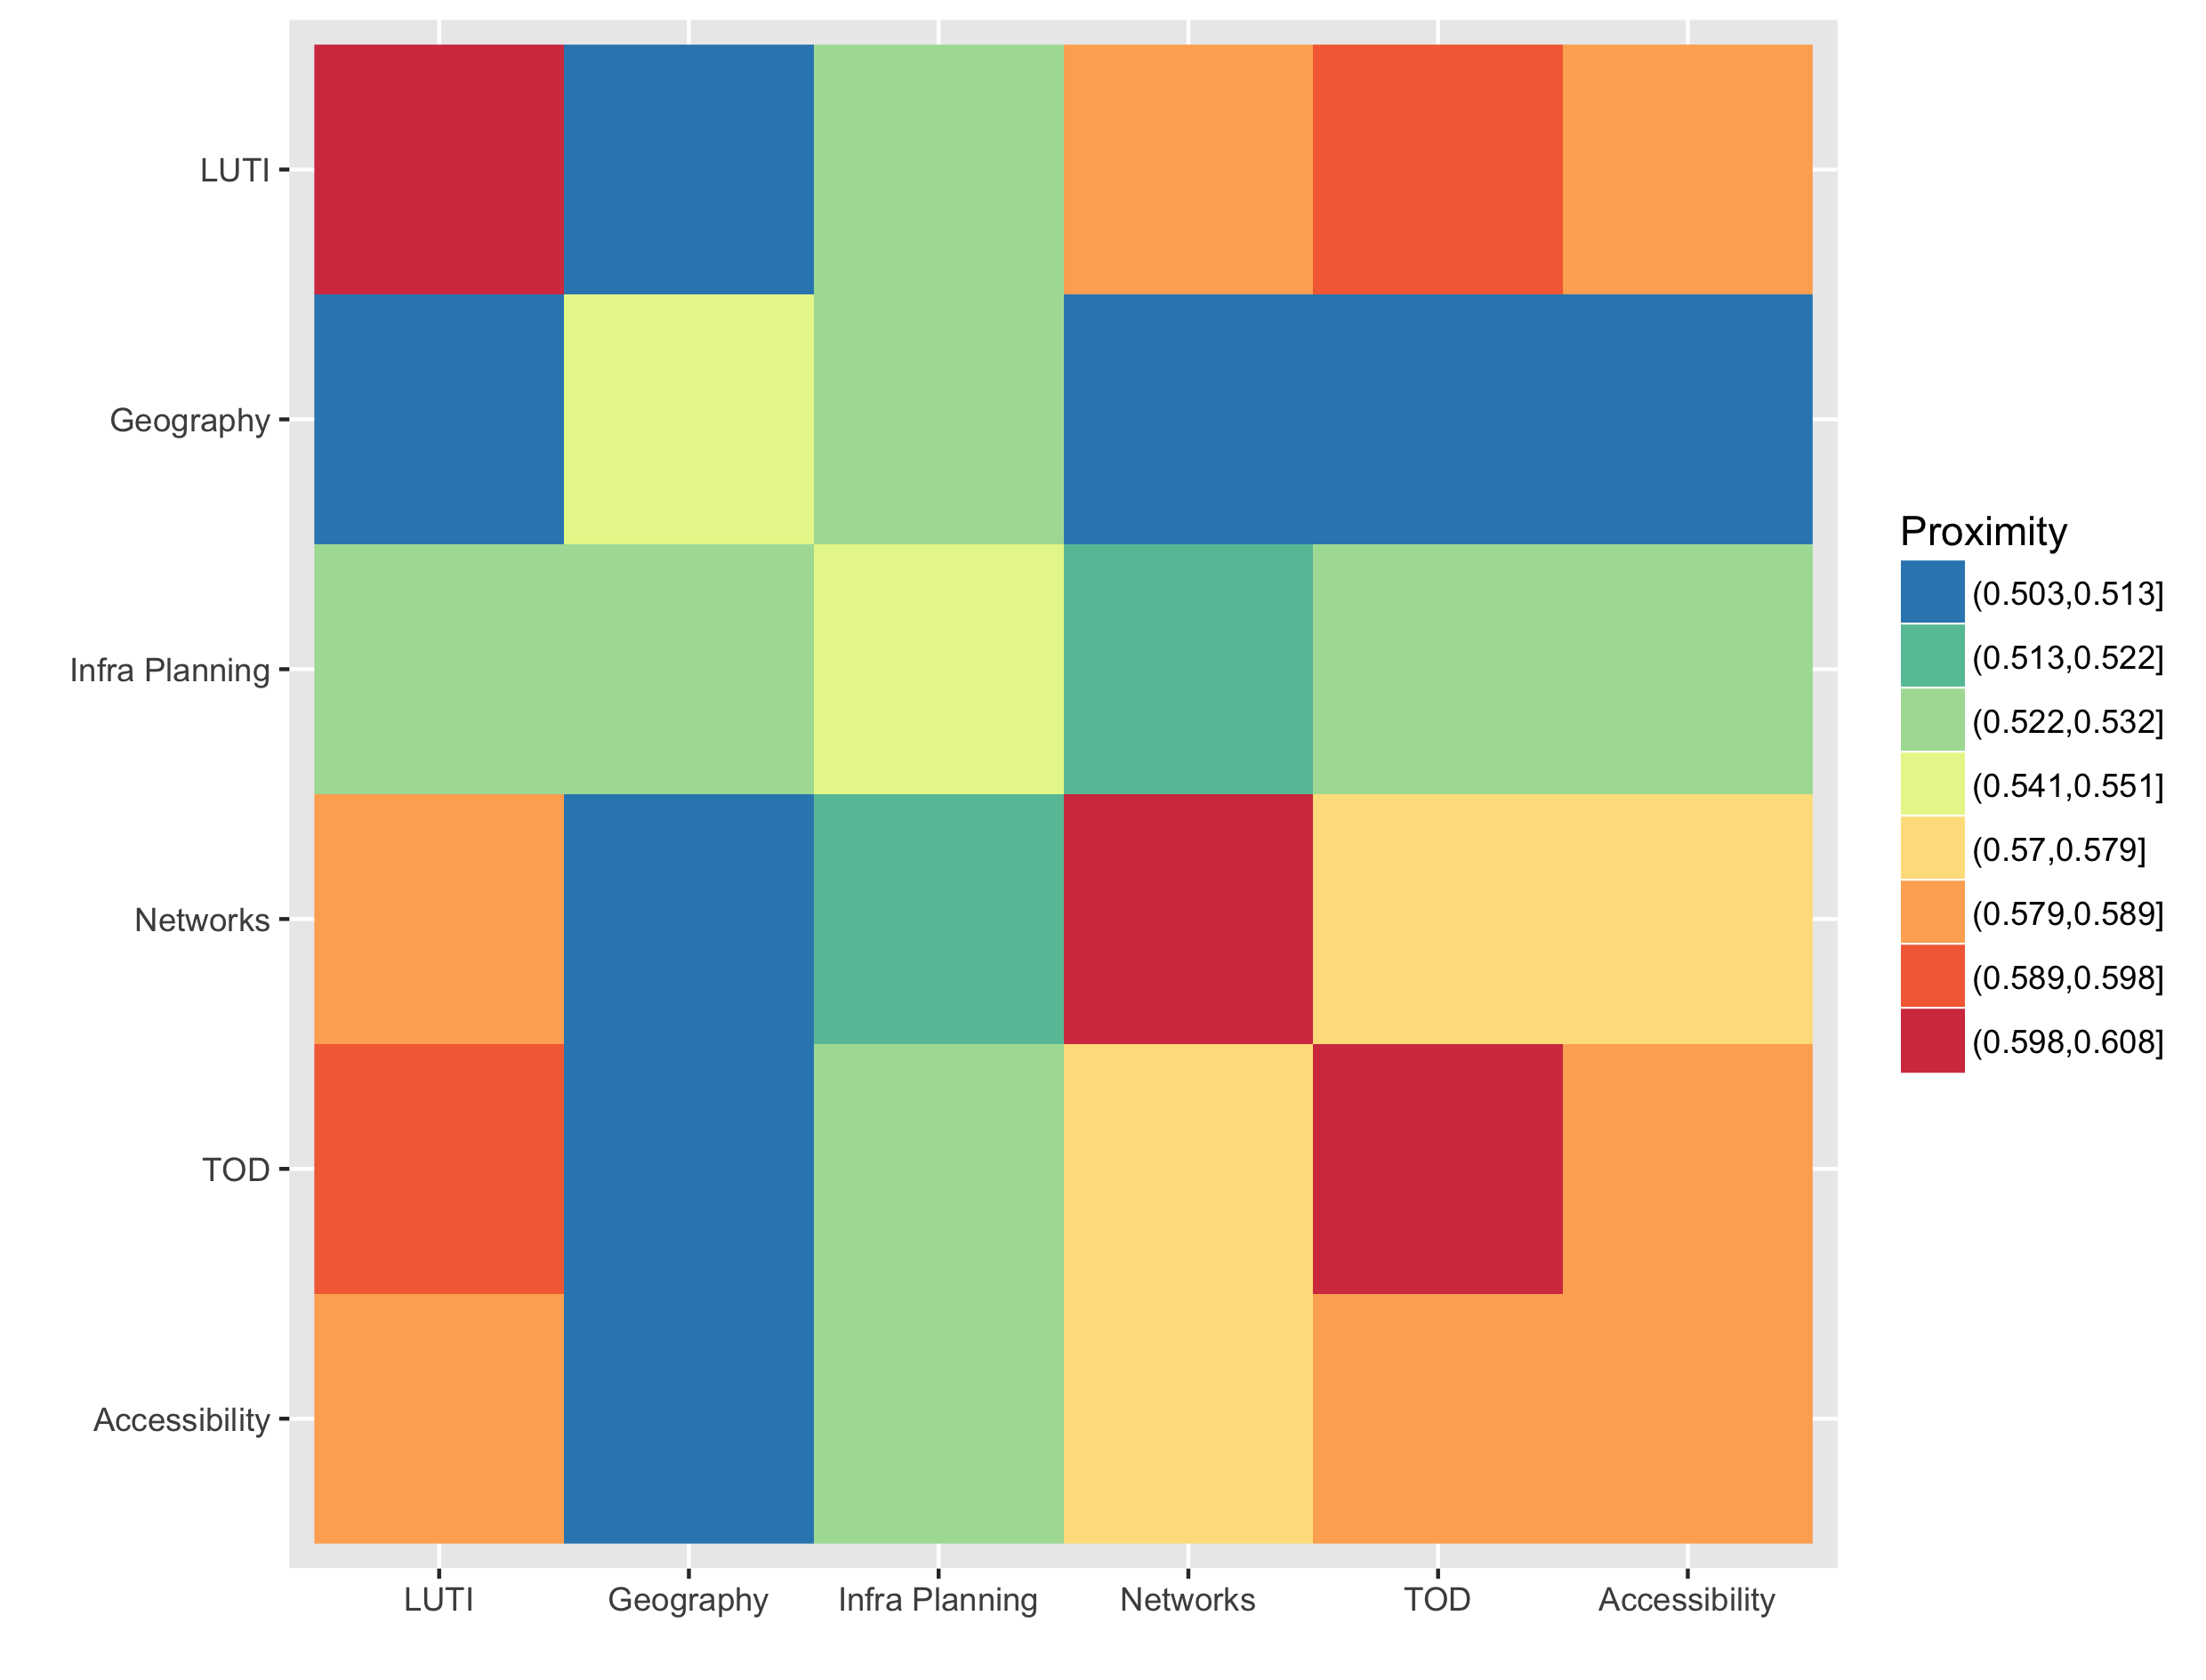
\includegraphics[width=0.49\linewidth]{Figures/QuantEpistemo/semantic_proximities}
\caption[][Motifs d'interdisciplinarité]{\label{fig:quantepistemo:interdisc}}{\textbf{Motifs d'interdisciplinarité.} \textit{(Haut Gauche)} Distribution des $I_i$ par classes de citations ; \textit{(Haut Droite)} Composition sémantiques des classes de citation ; \textit{(Bas Gauche)} Matrice de proximité de citation $c_{kk'}$ entre classes de citations ; \textit{(Bas Droite)} Matrice de proximité sémantique $s_{kk'}$ entre classes de citations.\label{fig:quantepistemo:interdisc}\comment[FL]{tu compares les disciplines entre elles mais pas la facon dont elles attaquent les questions au coeur de ta these. c'est dommage.}[(JR)c'est l'objet de la section suivante]}
\end{figure}
%%%%%%%%%%%%%%%%%%



% bootstrap
%min(corrs);max(corrs);mean(abs(corrs))
% -0.170952  0.5496791  0.08384802
% apply(bcorrs,2,mean)
%       minrho        maxrho    meanabsrho     minrhosup     maxrhosup meanabsrhosup 
%  -0.08792137    0.11690677    0.03137750   -0.17686637    0.68579406    0.11079253 
% apply(bcorrs,2,sd)
%       minrho        maxrho    meanabsrho     minrhosup     maxrhosup meanabsrhosup 
%  0.012683338   0.021324056   0.002250636   0.038402781   0.134996447   0.051553244 

% modularities
% sem : 0.1053156
% cit : 0.8140818
% bootstrap N=100
% sem : 0.073097051446193 +- 0.00307154703966512
% cit : 0.204223565075042 +- 0.0141450119581389


\bpar{
}{
Nous concluons cette analyse par une approche plus robuste pour quantifier les proximités entre couches de l'hyperréseau. Il est aisé de construire une matrice de corrélation entre deux classifications, par les corrélations de leur colonnes. Nous définissons les probabilités $\mathbf{P}_C$ toutes égales à 1 pour la classification de citation. La matrice de correlation de celle-ci avec $\mathbf{P}$ s'étend de -0.17 à 0.54 et a une moyenne de valeur absolue de 0.08, ce qui est significatif par rapport à des classifications aléatoire puisque un bootstrap à $b=100$ répétitions avec les matrices mélangées donne un minimum à $-0.08 \pm 0.012$, un maximum à $0.11 \pm 0.02$ et une moyenne absolue à $0.03 \pm 0.002$. Cela montre que les classifications sont complémentaires et que cette complémentarité est significative statistiquement par rapport à des classifications aléatoires. L'adéquation de la classification sémantique par rapport au réseau de citation peut également être quantifiée par la modularité multi-classes~\cite{nicosia2009extending} (voir~\ref{sec:app:patents} pour une définition mathématique), qui traduit la probabilité qu'un lien soit dû à la classification étudiée, en prenant en compte l'appartenance simultanée à de multiples classes. Ainsi, la modularité multi-classes des probabilités sémantiques pour le réseau de citation est de 0.10, ce qui d'une part est significativement signe d'adéquation, un bootstrap toujours à $b=100$ donnant une valeur de $0.073 \pm 0.003$, qui reste limitée vu la valeur maximale fixée par les probabilités de citations dans leur propre réseau qui donnent une valeur de 0.81, ce qui confirme d'autre part la complémentarité des classifications.
}








%--------------------------------------------------------------



%%%%%%%%%%%%%%%%%%%%%%%%
\subsection{Discussion}{Discussion}




\subsubsection{Towards modeling purpose and context automatic extraction}{Vers une modélisation des thèmes et une extraction automatique du contexte}


\bpar{
A possible direction to strengthen our quantitative epistemological analysis would be to work on full textes related to the modeling of interaction between networks and territories, with the aim to automatically extract thematics within articles. The idea would be to perform some kind of automatized modelography, with possible features to be extracted that would be ontologies, model architecture or structures, scales, or even typical parameter values. It is not clear to what degree structure of models can be extracted from their description in papers and it surely depends on the discipline considered. For example in a framed field such as transportation planning, using a pre-defined ontology (in the sense of dictionary) and a fuzzy grammar could be efficient to extract information as the discipline is relatively formatted. In theoretical and quantitative geography, beyond the barrier of language, information organisation is surely less subject to unsupervised data-mining because of the more literary nature of the discipline : synonyms and figures of speech are generally the norm in good level human sciences writing, fuzzing a possible generic structure of knowledge description. 
}{
Une direction possible pour renforcer cette analyse en épistémologie quantitative serait de travailler sur les textes complets des références contenant des efforts de modélisations des interactions entre réseaux et territoires, avec le but d'extraire automatiquement les thématiques des articles. Des méthodes plus adaptées pour les long texte que celle utilisée ici incluent par exemple l'Allocation Latente de Dirichlet~\cite{blei2003latent}. L'idée serait de procéder à une sorte de modélographie automatique, pour extraire des caractéristiques telle les ontologies, l'architecture ou la structure des modèles, les échelles ou même des valeurs typiques des paramètres. Il n'est pas clair dans quelle mesure la structure des modèles peut être extraite de leur description dans un article, et cela dépend sûrement de la discipline considérée. Par exemple dans champ relativement cadré comme la planification des transports, l'utilisation d'une ontologie pré-définie (dans le sens d'un dictionnaire) et d'une grammaire floue pourrait être efficace vu les conventions assez strictes dans la discipline. En géographie théorique et quantitative, au delà de la barrière du language\comment[FL]{?}, l'organisation de l'information est sûrement plus délicate à appréhender par de l'apprentissage non-supervisé à cause de la nature plus littéraire de la discipline : les synonymes et les figures de style sont généralement la norme pour l'écriture d'un bon niveau en sciences humaines, rendant plus floue une possible structure générique de la description des connaissances.
}


%Depending on extended results of the two previous sections and on thematic requirements (huge need of knowledge on precise models structure, that may appear when trying to construct more specialized operational models), this project may be conducted with more or less investment.




\subsubsection{Reflexivity}{Réflexivité}


\bpar{
The methodology developed here is particularly interesting since it is reflexive, i.e. it can be used on our work itself. Therefore, an other application will be the reflexivity of our thesis : we attend to proceed to similar analysis on our proper bibliography (and possibly its evolution, available via \texttt{git} history), to understand our patterns of knowledge, possible gaps or unveil unexpected developments. The detailed development is done in Appendix~\ref{app:reflexivity}.
}{
La méthodologie que nous avons développé ici est particulièrement intéressante puisqu'elle offre des potentialités de réflexivité, c'est à dire qu'elle peut être utilisée pour étudier notre approche elle-même. Une de ses applications, hors de celle à la revue scientifique Cybergeo dans la perspective de Science Ouverte (voir Appendice~\ref{app:sec:cybergeo}), sera à notre propre corpus de références, dans le but de révéler des possibles  directions de recherche ou problématiques exotiques. Il est éventuellement possible de le faire de manière dynamique, grâce à l'historique de \texttt{git} qui permet de récupérer n'importe quelle version de la bibliographie à une date donnée sur les trois ans écoulés. Il s'agira aussi de comprendre nos motifs de production de connaissance afin de contribuer à~\ref{sec:knowledgeframework}. Le développement détaillé est fait en Appendice~\ref{app:reflexivity}.
}





\stars




%
% 2.3 - Modelography



%-------------------------------

\newpage

\section{Systematic Review and Modelography}{Revue Systématique et Modélographie}




\comment[JR]{la modélographie doit logiquement arriver après les études d'épistemo quanti, qui ont permis de donner un aperçu de l'horizon scientifique}



An ongoing work is the production of a synthesis of this overview, from a modular modeling point of view, combined with a purpose and scale classification. Already mentioned, modular modeling consists in the integration of heterogeneous processes and implementation of processes in order to extract the set of mechanisms giving the best fit to empirical data~\cite{cottineau2015incremental}. We can thus classify models described here according to their building bricks in terms of processes implemented and thus identify possible coupling potentialities. This work is a preliminary step for the analysis in quantitative epistemology developed in chapter~\ref{ch:quantepistemo}.



%%%%%%%%%%%%%%%%%%%%
\subsection[Systematic Review][Revue Systématique]{Systematic Review and Meta-analysis}{Revue systématique et Meta-analyse}


Tandis que les études menées précédemment proposaient de construire un horizon global de l'organisation des disciplines s'intéressant à notre question, nous proposons à présent une étude plus ciblée des caractéristiques de modèles existants. Nous proposons pour cela dans un premier temps une revue systématique, c'est à dire la construction d'un corpus répondant à certaines contraintes, suivie d'une meta-analyse, c'est à dire une tentative d'explication de certaines caractéristiques des modèles par des modèles statistiques.

\comment[JR]{également tenter une classif endogène des modèles : selon les caractéristiques récupérées.}











%%%%%%%%%%%%%%%%%%%%
\subsection{Modelography}{Modélographie}


Nous passons à présent à une analyse mixte inspirée par les résultats précédents, notamment pour la classification. Elle a pour but d'extraire et de décomposer précisément les ontologies, échelles et processus, puis d'étudier des liens possibles entre ces caractéristiques des modèles et le contexte dans lequel ils ont été introduits. Il s'agit ainsi de la meta-analyse en quelque sorte, que nous désignerons ici par modélographie.



%%%%%%%%%%%%%%%%%
\begin{figure}
\centering
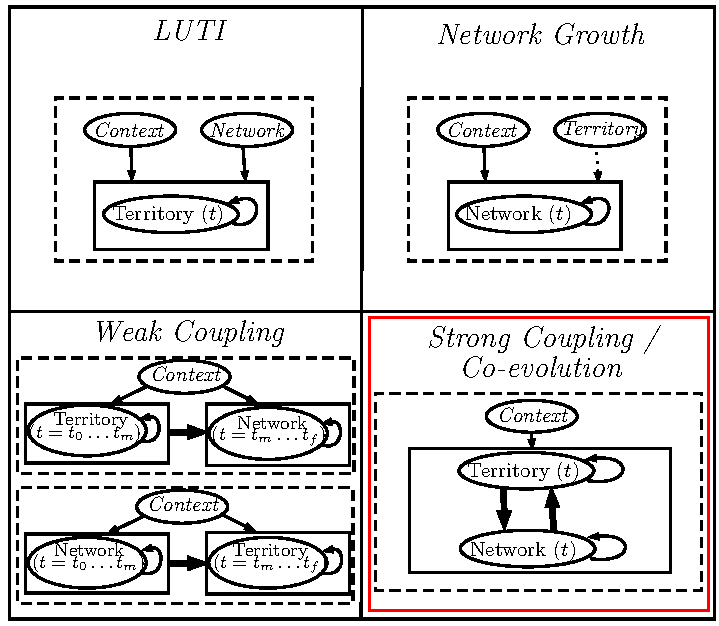
\includegraphics[width=\textwidth]{Figures/Modelography/coevolution}
\caption{}{Représentation schématique de la distinction entre différents types de modèles couplant territoires et réseaux.}
\end{figure}
%%%%%%%%%%%%%%%%%




caractéristiques : temporal and spatial span, scales, équilibre?, 


\todo{``bon choix'' de carac implique une bonne modularité de la classif obtenue dans une classif a priori (car on veut disciminer bien les modèles qu'on connait et qu'on juge différent) $\rightarrow$ faire une random forest regression et regarder structure endogène ; comparer à régressions simples.}









%%%%%%%%%%%%%%%%%%%%
\subsection{Discussion}{Discussion}

% préciser ici déjà des directions, clarifier question etc.













%
% Conclusion



%----------------------------------------------------------------------------------------

\newpage


\section*{Chapter Conclusion}{Conclusion du Chapitre}

La réflexivité, au sens de la reflexion de la recherche sur les facteurs influençant son contenu et sa propre structure, semble dans notre cas être nécessaire pour une appréhension claire des enjeux thématiques, méthodologiques et plus généralement scientifiques liés au processus que nous cherchons à modéliser : ceux-ci étant multi-scalaires, hybrides et hétérogènes, les angles d'approches et questionnements possibles sont nécessairement extrêmement variés, complémentaires et riche. Il pourrait s'agir d'une caractéristique fondamentale des systèmes socio-techniques, que \noun{Pumain} formule dans~\cite{pumain2005cumulativite} comme ``une nouvelle mesure de complexité'', qui serait liée aux nombre de point de vue nécessaires pour appréhender un système à un niveau donné d'exhaustivité. Cette idée rejoint la position de \emph{perspectivisme appliqué} que la section~\ref{sec:csframework} formalise et qui est implicitement présente dans l'investigation des relations entre Economie et Géographie développée en~\ref{app:sec:ecogeo}. Ainsi, la modélisation des interactions entre réseaux et territoires peut être reliées à un ensemble très large de disciplines et d'approches revues en section~\ref{sec:modelingsa}. Afin de mieux comprendre le paysage scientifique environnant, et quantifier les rôles ou poids relatifs de chacune, nous avons procédé à une série d'analyse en épistémologie quantitative en~\ref{sec:quantepistemo}. Une première analyse préliminaire basée sur une revue systématique algorithmique suggère un certain cloisonnement des domaines. Cette conclusion est confirmée par l'analyse d'hyperréseau couplant réseau de citation et réseau sémantique, qui permet également de dessiner plus finement les contours disciplinaires, à la fois sur leur relations directes (citations) mais aussi leur proximité scientifique pour les termes et méthodes utilisées. On peut alors utiliser le corpus constitué et cette connaissance des domaines pour une revue systématique semi-automatique et une meta-analyse en~\ref{sec:modelography}, qui permet de constituer un corpus de travaux traitant directement du sujet, qui est ensuite inspecté intégralement, permettant de lier caractéristique des modèles au différents domaines. On a alors à ce stade une idée assez précise de ce qui ce fait, pourquoi et comment. L'enjeu reste de déterminer les pertinences relatives de certaines approches ou ontologies, ce qui sera le but des trois chapitres de la deuxième partie. Nous concluons d'abord cette première partie par un chapitre de discussion~\ref{ch:positioning}, éclairant des points nécessaires à clarifier avant une entrée dans le vif du sujet.






\stars

%%%%%%%%%%%%%%%%%%%%%%%%%%%%%



%%%%%%%%%%%%%%%%%%%%%%%%%%%%%
% Chapter 3 : Positioning



% Chapter 

%\chapter{Positioning}{Positionnements} % Chapter title
\chapter{Positionnements}


\label{ch:positioning} % For referencing the chapter elsewhere, use \autoref{ch:name} 

%----------------------------------------------------------------------------------------

%\headercit{}{}{}

\comment[FL]{$\rightarrow$ a la fin}[(JR) pas d'accord car majoritairement pre-requis pour la suite]

\bigskip


Toute activité de recherche serait, selon certains acteurs de celle-ci, nécessairement politisée, de par pour commencer le choix de ses objets. Ainsi, \noun{Ripoll} alerte contre l'illusion d'une recherche objective et les dangers de la technocratie~\cite{ripoll2017jig}. Nous ne rentrerons pas dans ces débats bien trop vastes pour être traités même en un chapitre, puisqu'il rejoignent des thèmes de sciences politiques, d'éthique, de philosophie, liés par exemple à la gouvernance scientifique, à l'insertion de la science dans la société, à la responsabilité scientifique. Il est clair que même des sujets a priori intrinsèquement objectifs, comme la physique des particules et des hautes énergies, ont des implications regardant d'une part les choix de leur financements et les externalités associées (par exemple, l'existence du CERN a largement contribué au développement du calcul distribué), mais d'autre part aussi les applications potentielles des découvertes qui peuvent avoir des répercussions sociales considérables. En biologie, l'éthique est au coeur des principes fondateurs des disciplines, comme en témoignent les débats soulevés par l'émergence de la biologie synthétique~\cite{gutmann2011ethics}. Les tenants d'approche prudentes dans celle-ci se recoupent avec la biologie intégrative, or les Sciences Intégratives défendues par \noun{Paul Bourgine}, mises en oeuvre par l'intermédiaire du campus digital Unesco CS-DC\footnote{https://www.cs-dc.org/}, ont typiquement la responsabilité sociale et l'implication citoyenne au coeur de leur cercle vertueux. En Sciences Humaines et Sociales, comme les recherches interagissent avec les objets étudiés (en quelque sorte l'idée des \emph{interactive kind} de \noun{Hacking}~\cite{hacking1999social}), les implications politiques et sociales de la recherche sont bien évidemment indiscutables. Là où il y aurait matière à discussion, et nous y reviendrons en ouverture~\ref{ch:opening} car il s'agira d'une des questions ouvertes posées par notre recherche et sa démarche dans leur ensemble, serait sur la compatibilité des méthodes systématiques et \emph{evidence-based} avec les sciences sociales, autrement dit dans quelle mesure peut-on s'extraire de certains dogmatismes encore plus marqués lors de l'usage de théorie politiques\footnote{\noun{Monod} montre par exemple les désastres liés aux ``niaiseries épistémologiques'' découlant de l'application littérale de la dialectique matérialiste marxiste à l'épistémologie du vivant.}. Nous resterons ici à un niveau épistémologique, c'est à dire à des réflexions sur la nature et le contenu des connaissances scientifiques au sens large, c'est à dire co-construites et validées au sein d'une communauté imposant certains critères de scientificité, bien sûr évolutifs puisque nous nous positionnerons pour la systématisation de certains. Mais donc, même en restant à ce niveau, des prises de positions sont nécessaires, celles-ci pouvant être épistémologiques, méthodologiques, thématiques. Ces dernières ont déjà été ébauchée dans les deux chapitres précédents par les choix des objets d'étude, des problématiques, et seront renforcées à mesure de la progression pour finalement être synthétisées en Chapitre~\ref{ch:theory}. Nous proposons ici un exercice relativement original mais que nous jugeons nécessaire pour une lecture plus fluide de la suite, qui consiste en le développement précis de certains positionnements qui ont une influence particulière dans notre démarche de recherche. Par exemple, le travail en données quasi-intégralement ouverte et en architecture modulaire résulte de notre exigence de reproductibilité. L'utilisation des modèles et la manière de les explorer de notre vision du calcul intensif. Dans une première section (\ref{sec:reproducibility}), nous développons des exemples pour illustrer le besoin et la difficulté de reproductibilité, ainsi que les liens avec des nouveaux outils pouvant la favoriser mais aussi la mettre en danger. Dans une deuxième section (\ref{sec:computation}), nous argumentons sous forme d'essai pour un usage raisonné des données massives et du calcul intensif, et illustrons notre positionnement par rapport à l'exploration des modèles par une étude de cas méthodologique pour l'exploration de la sensibilité des modèles aux conditions initiales. Enfin, la dernière section (\ref{sec:epistemology}) explicite modestement des positions épistémologiques, notamment concernant le courant dans lequel nous nous plaçons, la complexité des objets en sciences sociales, et la nature de la complexité de manière générale. Le lecteur très familier avec les commandements de \noun{Banos}~\cite{banos2013pour} pourra éventuellement sauter les deux premières sections à part s'il est intéressé par des illustrations pratiques originales, notre positionnement étant très similaire et ne divergeant que sur des subtilités mineures pour les sujets évoqués dans ces sections.




\stars


\textit{Ce chapitre est composé de divers travaux. La première section est inédite. La deuxième section rend compte pour sa première partie du contenu théorique de \cite{raimbault2016cautious}, et pour sa deuxième partie des idées présentées dans \cite{cottineau2017initial}. La troisième section reprend dans sa première partie les bases épistémologiques de \cite{raimbault:halshs-01505084} approfondies par \cite{raimbault2017knowledge}, est inédite pour sa deuxième partie et rend compte de \cite{raimbault2017complex} pour sa dernière partie.
}







%
% 3.1 Reproducibility and Open Science




%----------------------------------------------------------------------------------------

\newpage

% Section : Reproducibility


\section{Reproducibility}{Reproducibilité}

\label{sec:reproducibility}


%----------------------------------------------------------------------------------------



\bpar{
The strength of science comes from the cumulative and collective nature of research, as progresses are made as Newton said ``standing on the shoulder of giants'', meaning that the scientific enterprise at a given time relies on all the work done before and that advances would not be possible without constructing on it. It includes development of new theories, but also extension, testing or falsifiability of previous ones.
}{
La force\comment[FL]{?} de la Science vient de la nature cumulative et collective de la recherche, puisque les progrès sont faits lorsque, comme \noun{Newton} l'a bien posé, on ``se tient sur les épaules de géants'', au sens que l'entreprise scientifique à un temps donné repose sur l'ensemble du travail précédent et qu'aucune avancée ne serait possible sans construire dessus. Cela inclut le développement de nouvelles théories, mais aussi l'extension, le test et la falsification de précédentes: l'avancée dans la construction de la tour signifie aussi la déconstruction de certaines briques obsolètes. Cet aspect de validation par les pairs et de remise en question constante est aussi ce qui légitime la Science pour une connaissance plus robuste et un progrès sociétal basés sur une connaissance d'un univers objectif, par rapport aux systèmes dogmatiques qu'ils soient politiques ou religieux~\cite{bais2010praise}. % note : pourrait introduire Monod ethique de la connaissance, pas le point.
}



\bpar{
The effective practice of reproducibility seems to be increasing~\cite{stodden2010scientific} and technical means to achieve it are always more developed (as e.g. ways to make data openly available, or to be transparent on the research process such as \texttt{git}~\cite{ram2013git}, or to integrate document creation and data analysis such as \texttt{knitr}~\cite{xie2013knitr}), at least in the field of modeling and simulation. However, the devil is indeed in the details and obstacles judged at first sight as minor become rapidly a burden for reproducing and using results obtained in some previous researches. We describe two cases studies where models of simulation are apparently highly reproducible but unveil as puzzles on which research-time balance is significantly under zero, in the sense that trying to exploit their results may cost more time than developing from scratch similar models.
}{
La reproductibilité semble être de plus en plus pratiquée de manière effective~\cite{stodden2010scientific} et les moyens techniques pour l'achever sont toujours plus développés (comme par exemple les outils pour déposer les données ouvertes, ou pour être transparent dans le processus de recherche comme \texttt{git}~\cite{ram2013git}, ou pour intégrer la création de document et l'analyse de données comme  \texttt{knitr}~\cite{xie2013knitr}), au moins dans le champ de la modélisation et de la simulation. Cependant le diable est bien dans les détails et des obstacles jugés dans un premier temps comme mineurs peuvent rapidement devenir un fardeau pour reproduire et utiliser des résultats obtenus dans des recherches précédentes. Nous décrivons deux études de cas où les modèles de simulation sont en apparence hautement reproductibles mais se révèlent vite des puzzles pour lesquels l'équilibre de temps de recherche passe rapidement sous zéro, au sens où essayer d'exploiter leur résultats coûtera plus en temps que de développer entièrement des modèles similaires.
}

\comment{\cite{2015arXiv150302388C}}

%We first propose to focus on the importance of reproducibility in science. More than a guideline, it is a way to practice science that a necessary condition for its rigour. Any non-reproducible work is not scientific.



%%%%%%%%%%%%%%%%%%%%%%%%%%%%%%%%%%
\subsection{Explicitation, documentation and implementation of models}{Explicitation, documentation et implémentation des modèles}




%%%%%%%%%%%%%%%%%%%%%%%%%%%%%%%%%%
\subsubsection{On the Need to Explicit the Model}{Sur le Besoin d'expliciter le modèle}


\bpar{
A current myth (to which we ourselves struggle to escape indeed) is that providing entire source code and data will be a sufficient condition for reproducibility. It will work if the objective is to produce exactly same plots or statistical analysis, assuming that code provided is the one which was indeed used to produce the given results. It is however not the nature of reproducibility. First, results must be as much implementation-independent as possible for clear robustness purposes. Then, in relation with the precedent point, one of the purposes of reproducibility is the reuse of methods or results as basis or modules for further research (what includes implementation in another language or adaptation of the method), in the sense that reproducibility is not replicability as it must be adaptable~\cite{drummond2009replicability}.
}{
Un mythe à la vie dure (auquel nous essayons en fait nous-même d'échapper) est que fournir le code source complet et les données seront une condition suffisante pour la reproductibilité, puisque la reproductibilité computationnelle complète implique un environnement similaire ce qui devient vite ardu à produire comme le montre~\cite{2016arXiv160806897H}. Pour résoudre ce problème, \cite{10.1371/journal.pone.0152686} propose l'utilisation de conteneurs Dockers qui permet de reproduire même le comportement de logiciels avec interface graphique independemment de l'environnement. C'est d'ailleurs une des direction courantes de développement d'OpenMole, pour simplifier le packaging des bibliothèques et des modèles en binaire (cf. \noun{R. Reuillon} dans~\cite{raimbault2017entretiens}). Dans tous les cas, le reproductibilité a des dimensions supplémentaires, il ne s'agit pas de l'objectif unique qui serait est de produire exactement les mêmes graphes et analyses statistiques, en supposant que le code fournit est celui qui a été effectivement utilisé pour produire les résultats donnés. Tout d'abord, doivent être autant que possible indépendants de l'implémentation (c'est à dire du langage, des bibliothèques, des choix de structures de données et de type de programmation) pour des motifs clairs de robustesse. Ensuite, en relation avec le point précédent, un des buts de la reproductibilité est la réutilisation des méthodes ou résultats comme base ou modules pour une recherche future (ce qui comprend une implémentation dans un autre langage ou une adaptation de la méthode), au sens que la reproductibilité n'est pas la possibilité stricte de répliquer car elle doit être adaptable~\cite{drummond2009replicability}.
}



\bpar{
Our first case study fits exactly that scheme, as it was undoubtedly aimed to be shared with and used by the community since it is a model of simulation provided with the Agent-Based simulation platform NetLogo~\cite{wilensky1999netlogo}. The model is also available online~\cite{de2007netlogo} and is presented as a tool to simulate socio-economic dynamics of low-income residents in a city based on a synthetic urban environment, generated to be close in stylized facts from the real town of Tijuana, Mexico. Beside providing the source code, the model appears to be poorly documented in the literature or in comments and description of the implementation. Comments made thereafter are based on the study of the urban morphogenesis part of the model (setup for the ``residential dynamics'' component) as it is our global context of study%~\cite{raimbault2014vers} % not really citable ?
. In the frame of that study, source code was modified and commented, which last version is available on the repository of the project\footnote{at \texttt{https://github.com/JusteRaimbault/CityNetwork/tree/master/Models/Reproduction/UrbanSuite}}.
}{
Notre premier cas d'étude suit exactement ce schéma, puisqu'il a sans aucun doute été conçu pour être partagé avec la communauté et utilisé, s'agissant d'un modèle de simulation fournit avec la plateforme de modélisation agent NetLogo~\cite{wilensky1999netlogo}. Le modèle est également disponible en ligne~\cite{de2007netlogo} et est présenté comme un outil pour simuler les dynamiques socio-économiques des résidents à bas revenus d'une ville au sein d'un environnement urbain synthétique, généré pour ressembler en terme de faits stylisés à la ville réelle de Tijuana, Mexico. Globalement, le modèle fonctionne de la façon suivante : (i) à partir de centre urbains, une distribution d'usage du sol est générée par modélisation procédurale similaire à \cite{lechner2006procedural}, c'est à dire des routes sont générées de proche en proche selon des règles géométriques et de hiérarchie locales, et un usage du sol ainsi qu'une valeur est attribué en fonction des caractéristique du patch (distance au centre, à la route) ; (ii) dans cet environnement urbain sont simulées des dynamiques résidentielles de migrants, qui cherchent à optimiser une fonction d'utilité dépendant du coût de la vie et de la configuration des autres migrants. A part fournir le code source, le modèle n'est que peu documenté dans la littérature ou dans les commentaires et la description de l'implémentation. Les commentaires qui suivent sont basés sur l'étude de la partie du modèle simulant la morphogenèse urbaine (setup pour la composante ``dynamiques résidentielles'') comme il s'agit de notre contexte global d'étude. Dans le cadre de cette étude, le code source a été modifié et commenté, dont la dernière version est disponible sur le dépôt du projet\footnote{at \texttt{https://github.com/JusteRaimbault/CityNetwork/tree/master/Models/Reproduction/UrbanSuite}}.
}



\paragraph{Rigorous Formalization}{Formalisation Rigoureuse}


\bpar{
An obvious part of model construction is its rigorous formalization in a formal framework distinct from source code. There is of course no universal language to formulate it~\cite{banos2013pour}, and many possibilities are offered by various fields (e.g. UML, DEVS, pure mathematical formulation). No paper nor documentation is provided with the model, apart from the embedded NetLogo documentation, that only thematically describes in natural language the ideas behind each step without developing more and provides information about role of different elements of the interface.
}{
Une partie évidente de la construction d'un modèle est sa formalisation rigoureuse dans un cadre formel distinct du code source. Il n'y a bien sûr aucun langage universel pour le formuler~\cite{banos2013pour}, et de nombreuses possibilités sont offertes par de nombreux champs (e.g. UML, DEVS, formulation mathématique pure), mais l'étape de formalisation précise, qui suit généralement une description plus intuitive donnant les idées et processus dominants (``rationelle''), ne peut pas être sautée. On pourrait se dire que le code source y est équivalent, mais ce n'est pas exactement vrai car on pourrait alors ne plus distinguer certains choix d'implémentation de la structure du modèle. Aucun article ni documentation n'accompagne le modèle ici, au delà de la documentation embarquée NetLogo, qui ne décrit que de manière thématique en langage naturel les idées derrière chaque étape sans plus développer et fournit de l'information sur le rôle des différents éléments de l'interface. Comme ces éléments manquent ici, le modèle n'est guère utilisable tel quel. On pourrait nous objecter ici que la partie que nous étudions est une procédure d'initialisation et non le coeur du modèle : nous maintenons que l'ensemble des procédures doit être également documenté et implémenté avec un soin équivalent, ou pointer vers une référence extérieure dans le cas d'utilisation d'un modèle tiers, comme nous le faisons d'ailleurs pour le couplage effectué en~\ref{sec:computation}.
}



\bpar{
This formulation is a key for it to be understood, reproduced and adapted; but it also avoids implementation biases such as
\begin{itemize}
\item Architecturally dangerous elements: in the model, world context is a torus and agents may ``jump'' in the euclidian representation, what is not acceptable for a 2D projection of real world. To avoid that, many tricky tests and functions were used, including unadvised practices (e.g. dead of agents based on position to avoid them jumping).
\item Lack of internal consistence: the example of the patch variable \texttt{land-value} used to represent different geographical quantities at different steps of the model (morphogenesis and residential dynamics), what becomes an internal inconsistence when both steps are coupled when option \texttt{city-growth?} is activated.
\item Coding errors: in an untyped language such as NetLogo, mixing types may conduct to unexpected runtime errors, what is the case of the patch variable \texttt{transport} in the model (although no error occurs in most of run configurations from the interface, what is more dangerous as the developer thinks implementation is secure). Such problems should be avoided if implementation is done from an exact formal description of the model.
\end{itemize}
}{
Une telle formulation est essentielle pour que le modèle soit compris, reproduit et adapté ; mais elle évite également des biais d'implémentation comme
\begin{itemize}
\item Des éléments architecturaux dangereux : le contexte du monde est une sphère, ce qui n'est pas raisonnable pour ce modèle à l'échelle d'une ville, les mesures de proximité jouant un rôle important dans les processus de production de la forme urbaine. Les agents peuvent ``sauter''\comment[FL]{sens ?} dans la représentation euclidienne, ce qui n'est pas acceptable pour une projection en deux dimensions du monde réel. Pour éviter cela, de nombreux tests et fonctions subtils sont utilisés, incluant des pratiques déconseillées (e.g. mort d'agents basée sur leur position pour les empêcher de sauter).
\item Manque de cohérence interne : par exemple la variable de patch \texttt{land-value} \comment[AB]{ces variables sont-elles définies quelque part ? Si oui, le préciser. Sinon, revoir ton argumentation…} utilisée pour représenter différentes quantités géographiques à différentes étapes du modèle (morphogenèse et dynamiques résidentielles), ce qui devient une incohérence interne quand les deux étapes sont couplées lorsque l'option permettant de faire croître la ville est activée.
\item Erreur de code : dans un langage non typé comme NetLogo, le mélange des types peut conduire à des erreurs inattendues à l'execution, ou même des \emph{bugs} non détectables directement et alors plus dangereux. C'est le cas de la variable de patch \texttt{transport}\comment[AB]{idem} dans le modèle (même si aucune erreur ne survient dans la majorité des configurations depuis l'interface, ce qui est plus dangereux comme le développeur pense que l'implémentation est sûre). De tels problèmes devraient être évités si l'implémentation est faite à partir d'une description exacte du modèle.
\end{itemize}
}

\paragraph{Transparent Implementation}{Implémentation Transparente}


\bpar{
A totally transparent implementation is expected, including ergonomics in architecture and coding, but \ldots
}{
Une implémentation totalement transparente doit être attendue, incluant une certaine ergonomie dans l'architecture et le code, mais aussi dans l'interface et la description du comportement attendu du modèle.
}

\paragraph{Expected Model Behavior}{Comportement attendu du modèle}


\bpar{
Whatever the definition, a model can not be reduced to its formulation and/or implementation, as expected model behavior or model usage can be viewed as being part of the model itself. In the frame of \noun{Giere}'s perspectivism~\cite{giere2010scientific}, the definition of model includes the purpose of use but also the agent who aims to use it. Therefore a minimal explication of model behavior and exploration of parameter roles is highly advised to decrease chances of misuses or misinterpretations of it. It includes simple runtime charts that are immediate on the NetLogo platform, but also indicators computations to evaluate outputs of the model. It can also be improved visualizations during runtime and model exploration, such as showed in Fig.~\ref{fig:example_tij_viz}.
}{
Quelle que soit la définition, un modèle ne peut pas être réduit à sa formulation et/ou implémentation, comme le comportement attendu ou l'utilisation du modèle peuvent être vu comme des parties du modèle lui-même. Dans le cadre du perspectivisme de \noun{Giere}~\cite{giere2010scientific}, la définition du modèle inclut le motif de l'utilisation mais aussi l'agent qui vise à l'utiliser. Pour cela une explication minimale du comportement du modèle et une exploration du rôle des paramètres sont fortement recommandés pour diminuer les chances de mauvais usage ou mauvaises interprétations de celui-ci. Cela inclut des graphes simples obtenus immédiatement à l'exécution sur la plateforme NetLogo, mais aussi un calcul d'indicateurs pour évaluer les sorties du modèle. Il peut aussi s'agir de visualisations améliorée pendant l'execution et l'exploration du modèle, comme le montre la figure~\ref{fig:example_tij_viz}.
}


%%%%%%%%%%%%%%%%%%%%%
\begin{figure}[h!]
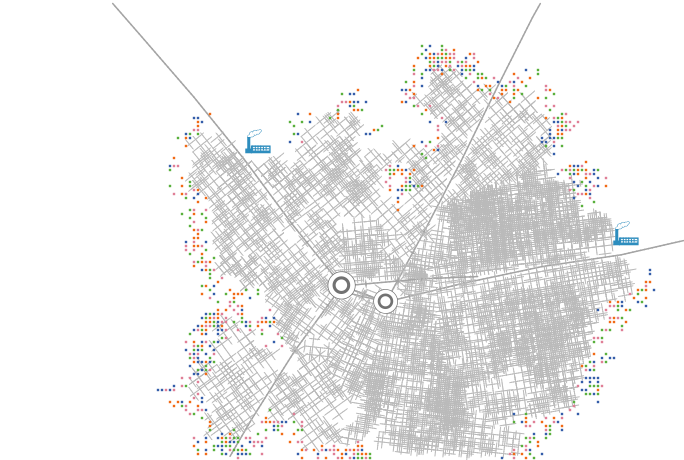
\includegraphics[width=0.3\linewidth]{Figures/Reproducibility/stdView}
\hfill
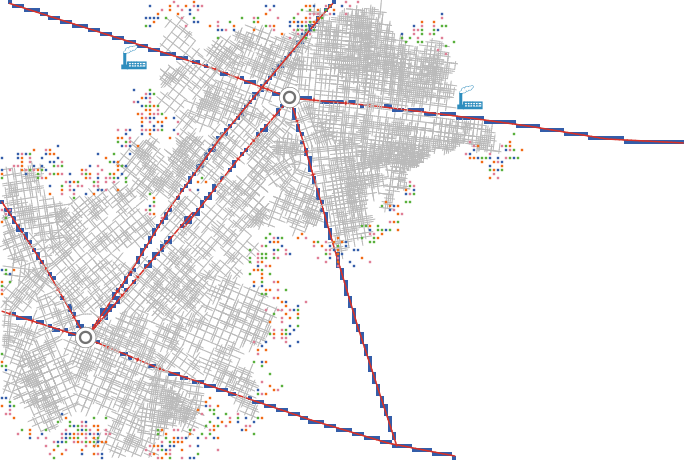
\includegraphics[width=0.3\linewidth]{Figures/Reproducibility/ViewRoads}
\hfill
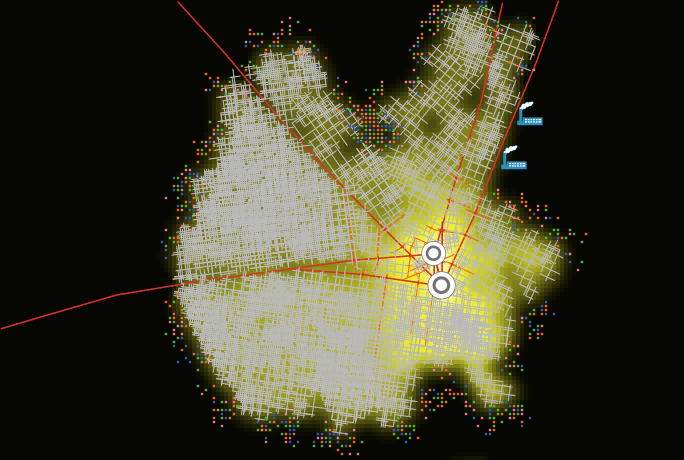
\includegraphics[width=0.3\linewidth]{Figures/Reproducibility/landValues_cityFinished}
\caption[Reproducibility and visualization][Reproductibilité et visualisation]{Example of simple improvement in visualization that can help understanding mechanisms implied in the model. \textit{Left: } Example of original output ; \textit{Middle: } Visualization of main roads (in red) and underlying patches attribution, suggesting possible implementation bias in the use of discretized trace of roads to track their positions ; \textit{Right: }Visualization of land values using a more readable color gradient. This step confirms the hypothesis, through the form of value distribution, that the morphogenesis step is an unnecessary detour to generate a random field for which simple diffusion method should provide similar results, as detailed in the paragraph on implementation.\label{fig:example_tij_viz}}{\textbf{Exemple d'amélioration simple dans la visualisation qui peut aider à appréhender les mécanismes impliqués par le modèle.} (Gauche) Exemple de sortie originale ; (Centre) Visualisation des routes principales (en rouge) et de l'attribution des patches sous-jacente, qui suggère de possibles biais d'implémentation dans l'utilisation de la trace discrete des routes pour garder trace de leur position ; (Droite) Visualisation des valeurs foncières en utilisant un gradient de couleur plus lisible. Cette étape confirme l'hypothèse, par la forme de la distribution des valeurs, que l'étape de morphogenèse est un détour non-nécessaire pour générer un champ aléatoire pour lequel des simples mécanismes de diffusion devrait fournir des résultats similaires, comme détaillé dans le paragraphe sur l'implémentation. Initialement, l'interface du modèle ne permet pas ces options de visualisation, ces à dire se limite à la première image. On ne peut se rendre compte des processus en jeu pour la morphogenèse, liés aux patches de route et au valeurs foncières se diffusant.\label{fig:example_tij_viz}}
\end{figure}
%%%%%%%%%%%%%%%%%%%%%



%%%%%%%%%%%%%%%%%%%%%
\subsubsection{On the Need of Exactitude in Model Implementation}{Sur le besoin d'exactitude dans l'implémentation du modèle}


\bpar{
Possible divergences between model description in a paper and the effectively implemented processes may have grave consequences on the final reproducibility. The road network growth model given in~\cite{barthelemy2008modeling} is one example of such a discrepancy. A strict implementation of model mechanisms provide slightly different results than the one presented in the paper, and as source code is not provided we need to test different hypotheses on possible mechanisms added by the programmer (that seems to be a connexion rule to intersections under a certain distance threshold). Lessons that could be possibly drawn from this examples are 
\begin{itemize}
\item the necessity of providing source code
\item the necessity of providing architecture description along with code (if model description is in a langage too far from architectural specifications) in order to identify possible implementation biaises
\item the necessity of performing and detailing explicitly model explorations, that would in that case have helped to identify the implementation bias.
\end{itemize}
}{
Des divergences potentielles entre la description du modèle dans un article et les processus effectivement implémentés peut avoir des conséquences graves sur la reproductibilité finale. Le modèle de croissance du réseau routier donné dans~\cite{barthelemy2008modeling} est un exemple d'un tel décalage. Une implémentation stricte des mécanismes du modèle produit des résultats légèrement différents de ceux présentés dans le papier, et comme le code source n'est pas fourni nous devrions tester différentes hypothèses sur des mécanismes possibles ajoutés par le programmeur (qui semble être une règle de connexion aux intersections sous un certain seuil de distance). Des leçons qui peuvent éventuellement être tirées de cet exemple, qui rejoignent partiellement mais complètent celle tirées dans l'étude de cas précédente, sont
\begin{itemize}
\item la nécessité de fournir le code source
\item la nécessité de fournir une description de l'architecture en même temps que le code (si la description du modèle est faite dans un langage trop loin de spécification architecturales) afin d'identifier des biais possibles d'implémentation
\item la nécessité de procéder à des explorations explicites du modèle et de les détailler, ce qui dans ce cas aurait permis d'identifier de possibles biais d'implémentation.
\end{itemize}
}



\bpar{
Making the last point mandatory may ensure a limited risk of scientific falsification as it is generally more complicated to fake false exploration results than to effectively explore the model. One could imagine an experiment to test the general behavior of a subset of the scientific community regarding reproducibility, that would consist in the writing of a false modeling paper in the spirit of~\cite{zilsel2015canular}, in which opposite results to the effective results of a given model are provided, without providing model implementation. A first bunch of test would be to test the acceptance of a clearly non-reproducible paper in diverse journals, possibly with a control on textual elements (using or not ``buzz-words'' associated to the journal, etc.). Depending on results, a second experiment may be tested with providing open source code for model implementation but still with false results, to verify if reviewers effectively try to reproduce results when they ask for the code (in reasonable computational power limits of course, HPC being not currently broadly available in Humanities).
}{
Rendre le dernier point obligatoire pourrait assurer un risque limité de falsification puisqu'il est généralement plus compliqué de falsifier des résultats d'exploration plutôt que d'explorer effectivement le modèle. On pourrait imaginer une expérience pour tester le comportement général d'un sous-ensemble de la communauté scientifique au regard de la reproductibilité, qui consisterait en l'écriture d'un faux papier de modélisation dans l'esprit de \cite{zilsel2015canular}, dans lesquels des résultats opposés aux résultats effectifs d'un modèle donné seraient fournis, sans fournir l'implémentation du modèle. Un premier test serait de tester l'acceptation d'un papier clairement non reproductible dans divers journaux, si possible avec un contrôle sur les éléments textuels (par exemple en utilisant ou non des ``buzz-words'' chers au journal). Selon les résultats, une expérience plus poussée serait de fournir l'implémentation open source mais toujours avec des résultats modifiés plus ou moins fortement, afin de tester si les reviewers essayent effectivement de reproduire les résultats quand ils demandent le code (dans des capacités de calcul limitées bien sûr, le HPC n'étant pas encore largement disponibles en sciences sociales). Notre intuition est que les résultats obtenus seraient fortement négatifs, vu les difficultés rencontrées par une exigence de discipline de reproduction indépendante lors de nombreuses relectures, même pour des revues faisant de la reproductibilité une condition \emph{sine qua non} de la publication, les auteurs trouvant des astuces pour se dérober aux contraintes (postuler que des données de simulation ne sont pas des données, ne fournir qu'une version agrégée inutile du jeu de données utilisées, etc. ; nous reviendrons sur le rôle des données plus loin).
}






%%%%%%%%%%%%%%%%%%%%%
\subsection{Interactive Exploration and Production of Results}{Exploration interactive et production des résultats}

L'usage d'applications interactives pour la fouille de données a des avantages non discutables, tel qu'une familiarisation avec la structure des données par une vue d'ensemble qui serait beaucoup plus laborieuse voire impossible autrement. C'est la même idée sous-jacente qui justifie l'interactivité pour l'exploration préliminaire des modèles basé-agent intégrée à des plateformes comme Netlogo~\cite{wilensky1999netlogo} ou Gamma [Cit. gamma]. C'était d'ailleurs un objectif couplé qu'avait initialement~\cite{rey2015plateforme}, c'est à dire une intégration complète de l'exploration fine des modèles et de la production des graphes de sortie ainsi que leur exploration interactive. Comme le rappelle R. Reuillon (Entretien du 11/04/2017, voir \ref{app:data:interview}), la plateforme OpenMole qui devait accueillir cette couche supplémentaire était à ses débuts à l'époque et ne l'est toujours pas aujourd'hui, puisque l'état de l'art de telles pratiques est en pleine construction et bouleversements réguliers~\cite{holzinger2014knowledge}. Des difficultés au regard de la reproductibilité, qui nous concernent particulièrement ici, sont récurrentes et loin d'être résolues. En effet, il faut bien situer la position de ces outils et méthodes comme une aide cognitive préliminaire\footnote{que nous ne jugeons pas superficielle puisque nous les mobilisons au moins par deux fois par la suite, voir \ref{sec:transportationequilibrium} et \ref{sec:energyprice}}, mais peu souvent comme permettant la production de résultats finaux : lorsque les paramètres ou dimension se multiplient, l'export d'un graphe est bien souvent déconnecté de l'information complète ayant conduit à sa production. De la même manière, l'utilisation de notebooks intégrés tel Jupyter, permettant d'intégrer analyses et rédaction du compte-rendu, peut devenir dangereux car on peut justement revenir sur un script, tester différentes valeurs d'un paramètre, et perdre les valeurs qui avaient produit un graphe donné. L'utilisation de versioning peut être une solution partielle mais souvent lourde. Dans l'idéal, tout logiciel interactif permettant l'export de résultats devrait en même temps exporter un script ou une description exacte et utilisable permettant d'arriver exactement à ce point à partir des données brutes. La plupart des applications d'exploration interactives de données spatio-temporelles sont à ce regard relativement immatures scientifiquement, car même dans le cas où elles sont totalement honnêtes et transparentes sur les analyses présentées à l'utilisateur, ce qui n'est malheureusement pas la règle, les tâtonnements d'exploration progressive ne sont pas reproductibles et la méthode d'extraction de caractéristiques est ainsi relativement aléatoire. En poussant le raisonnement, leur utilisation révélerait plutôt l'aveu d'une faiblesse d'un manque de méthodes systématiques accompagnant la découverte de motifs dans des données spatio-temporelles complexes de manière efficace. De manière très visionnaire, \noun{Banos} avait déjà mis en garde contre ``les dangers de la jungle'' des données dans~\cite{banos2001propos}, quand il souligne très justement que l'exploration interactive doit nécessairement se doubler d'indicateurs locaux adaptés, mais surtout d'outils d'exploration automatisés et de critère d'évaluation des choix faits et des motifs découverts par l'utilisateur. On revient encore à l'idée d'une plateforme intégrée dont OpenMole pourrait être un précurseur. La combinaison des capacités cognitives humaines au traitement machine, notamment pour des problèmes de vision par ordinateur, ouvre des possibilités de découvertes inédites, encore plus via une utilisation collective comme en témoigne le Galaxy Zoo~\cite{2010AEdRv...9a0103R}. Les résultats d'un crowdsourcing de la cognition humaine peuvent rivaliser avec les techniques automatiques les plus avancées comme le montre~\cite{10.1371/journal.pone.0178165} pour l'exemple de la comparaison de cartes spatiales. Ces possibilités ne doivent cependant pas être sur-estimées ou utilisées à mauvais escient, et les questions d'intégration efficiente homme-machine sont d'ailleurs totalement ouvertes. Dans le domaine de la visualisation de l'information géographique, \cite{pfaender2009spatialisation} introduit une sémiologie spécifique visant à favoriser l'exploration de grands jeux de données hétérogènes, et l'expérimente sur une application spécifique : il s'agit d'une avancée considérable vers une plateforme intégrée et une exploration interactive saine et reproductible, les directions d'exploration répondant à des modèles basés sur les sciences cognitives. 






%%%%%%%%%%%%%%%%%%%%%
\subsection{Perspectives}{Perspectives}


\bpar{
Again, reproducibility and transparency is a non-negotiable feature of contemporaneous science, along with Open practices and Open Access. Too much examples (see a very recent one in experimental economics~\cite{camerer2016evaluating}) show in various disciplines the lack of reproducibility of experiments, that is a falsification of previous results or a result in itself. Falsification is a costly practice, and even if necessary~\cite{chavalarias2005nobel}, could be made more efficient through more transparency and direct reproducibility, increase therein the global workflow of science. We develop in parallel of this thesis various tools aimed to ease reproducibility, for which an overview is given in appendix~\ref{app:workflow}.
}{
Encore une fois, la reproductibilité et la transparence sont des éléments essentiels incontournables de la science contemporaine, liés aux pratiques de science ouverte et d'accès ouvert. Beaucoup d'exemples (voir un récent en économie expérimentale dans~\cite{camerer2016evaluating}) dans diverses disciplines montrent le manque de reproductibilité des résultats des expériences, alors que celle ci doit pouvoir conduire à une falsification ou à une confirmation de ces résultats. La falsification est une pratique coûteuse car demandant un certain investissement au détriment de sa propre recherche~\cite{chavalarias2005nobel}. Elle pourrait ainsi être rendue plus efficiente grâce à une transparence augmentée. Des outils spécialement dédiés à une reproductibilité directe, souvent permise par l'ouverture, devraient accroître la performance globale de la science. Mais l'accès ouvert a des impacts bien plus large que la science elle-même : \cite{2015arXiv150607608T} montre un transfert des connaissances scientifiques accru vers la société dans le cas d'articles ouverts, notamment par des intermédiaires comme Wikipedia.
}

Le développement et la systématisation de standards et de bonnes pratiques, de manière conjointe sur les différentes problématiques évoquées, est une condition nécessaire à une rigueur scientifique qui devrait être uniforme au travers de l'ensemble des disciplines existantes. Nous construisons par exemple des exemples d'outils facilitant le flot de production scientifique, ceux-ci étant détaillés en Appendice~\ref{app:workflow}. Par exemple, pour les sciences computationnelles, on a déjà évoqué les potentialités de l'utilisation de \texttt{git} qui s'étendent en fait sans contrainte de disciplines ni de types de recherche si les bonnes adaptations sont introduites. Le suivi précis de l'ensemble des étapes d'un projet, gardé en historique offrant la possibilité de revenir à n'importe laquelle à tout moment, mais aussi de travailler de façon collaborative, plus ou moins parallèlement selon les besoins en utilisant les branches, est un exemple de service fourni par cet outil. Un exemple de bonnes pratiques d'utilisation est donné par~\cite{10.1371/journal.pcbi.1004947}. Plus généralement, les sciences computationnelles nécessitent l'adoption de certains standards et pratiques pour assurer une bonne reproductibilité, et ceux-ci restent majoritairement à développer : \cite{wilson2017good} donne des premières pistes. Concernant la qualité des données, de nombreux efforts sont faits pour introduire des cadres de standardisation des données : par exemple~\cite{10.1371/journal.pone.0178731} décrit un cadre conceptuel visant à guider la résolution de problème récurrent liés à la qualité des données de biodiversité (comme par exemple évaluer des mesures jugeant de l'usage possible d'un jeu de données pour un problème donné).

\comment{citer Romain sur le blockchain, en lien avec ce papier ? \cite{2017arXiv170706552}}


L'accès aux données est également un point crucial pour la reproductibilité, et sans nous y attarder car cela impliquerait des développements sur la définition, la philosophie, le droit des données etc. qui sont des sujets de recherche en eux-même, nous donnons des perspectives sur les potentiels d'une ouverture systématique des données en recherche. En géographie, les \emph{data paper} sont une pratique inexistante, et la règle est plutôt de garder la main jalousement sur un jeu produit, capitalisant sur le fait d'être le seul à y avoir accès. Il est évident que la qualité et quantité des connaissances produites sera nécessairement plus grande si un jeu de données est publiquement ouvert, puisqu'au moins la même chose sera obtenue, et on peut s'attendre à une prise en main par d'autres domaines, d'autres méthodes, et donc à une plus grande richesse. La fermeture induira plutôt des effets négatifs, comme par exemple du temps perdu à recoder un base vectorielle donnée uniquement sous forme de carte dans un article. L'argument du temps passé comme justification à la fermeture est absurde, puisqu'au contraire, en voyant les données comme une composante à part entière de la connaissance (voir le cadre de connaissances en~\ref{sec:knowledgeframework}), le temps passé doit impliquer plus de citations, donc plus d'utilisation, ce qui passe nécessairement par l'ouverture pour des données. De même, quelle logique, sinon la même absurde de propriété des connaissances, pousse les géographes à insérer un copyright sur l'ensemble de leurs cartes mais aussi leurs figures, jusqu'à un copyright pour un simple histogramme qui s'en serait bien passé si on avait pu l'interroger, honnête de simplicité ? Une expérience de revue induit à réellement s'inquiéter sur la valeur donnée à l'ouverture des données par les auteurs : au bout d'une dizaine d'articles, incluant des journaux affichant comme priorité et pré-requis l'ouverture totale des données et modèles, dont un seul est seulement partiellement ouvert et l'ensemble des autres implique de croire sur parole les résultats présentés (alors qu'un des but de la revue est de contourner les biais cognitifs qu'un ou des humains ont forcément par une validation croisée qui doit se faire sur les résultats bruts et non des interprétations contenant ces biais), il est difficile de croire que des mutations profondes des pratiques ne sont pas nécessaire. Mais en suivant l'adage de Framasoft, ``la route est longue mais la voie est libre'', les perspectives sont nombreuses pour une évolution dont la lenteur n'est pas inéluctable. Le journal Cybergéo, pionnier des pratiques d'ouverture en sciences sociales (première revue entièrement électronique, première revue à lancer une rubrique de \emph{model papers}), lance en 2017 une rubrique \emph{data papers} visant à inciter le développement du partage de données et de l'ouverture en géographie. Il reste des zones grises sur lesquelles il est impossible aujourd'hui d'avoir des perspectives, notamment le droit des données. On peut citer des exemples parmi les études empiriques que nous développons : les données bibliographiques sont obtenues au prix d'une guerre de blocage par Google et un effort considérable pour la gagner ; les données immobilières proviennent d'une base propriétaire achetée avec de l'argent public, et nous pouvons profiter d'un flou du contrat pour les rendre disponibles de manière agrégées avec les résultats ; les données des stations essence proviennent d'une source dont la légalité ne devrait pas être creusée plus, et nous ne pouvons malheureusement pas les rendre disponibles sans prendre de risques - cet aspect n'a cependant jamais fait broncher les reviewers qui n'ont même pas mentionné le manque d'accès aux données. L'ouverture implique un engagement qui fait résolument partie de nos positionnements. C'est la même idée qui soutient la construction de l'application \texttt{CybergeoNetworks}\footnote{\texttt{http://shiny.parisgeo.cnrs.fr/CybergeoNetworks}}, qui couple les outils présentés en~\ref{sec:quantepistemo} avec d'autres approches complémentaires d'analyse de corpus, dans le but d'encourager la réflexivité scientifique, et de mettre cet outil ouvert à la disposition d'éditeurs indépendants, pour s'émanciper de la nouvelle main mise des géants de l'édition qui à la recherche d'un nouveau modèle pour sécuriser leur profits parient sur la vente de meta-contenu et de son analyse. Heureusement, la récente loi numérique en France a gagné le bras de fer contre leur revendication d'un droit exclusif sur la fouille de texte complets.

%inserer lien vers residential dynamics repo ? % NON



\stars



% 3.2 Big Data, Computation and Model Exploration





%----------------------------------------------------------------------------------------

\newpage



\section[Computation and Model Exploration][Calcul Intensif et Exploration des Modèles]{Big Data, Computation and Model Exploration}{Données Massives, Calcul Intensif et Exploration des Modèles}

\label{sec:computation}


%----------------------------------------------------------------------------------------



Nous nous positionnons à présent sur les questions liées à l'utilisation des données massives et du calcul intensif, ce qui induit par extension une réflexion sur les méthodes d'exploration de modèles. Il n'est pas évident que ces nouvelles possibilités soient nécessairement accompagnées de mutations épistémologiques profondes, et nous montrons au contraire que leur utilisation nécessite plus que jamais un dialogue avec la théorie. Implicitement, cette position préfigure le cadre épistémologique pour l'étude des Systèmes Complexes dont nous donnons le contexte à la section suivante~\ref{sec:epistemology} et que nous formalisons en ouverture~\ref{sec:knowledgeframework}.



\subsection{For a cautious use of big data and computation}{Pour un usage raisonné des données massives et de la computation}

\bpar{
The so-called \emph{big data revolution} resides as much in the availability of large datasets of novel and various types as in the always increasing available computational power. Although the \emph{computational shift} (\cite{arthur2015complexity}) is central for a science aware of complexity and is undeniably the basis of future modeling practices in geography as \cite{banos2013pour} points out, we argue that both \emph{data deluge} and \emph{computational potentialities} are dangerous if not framed into a proper theoretical and formal framework. The first may bias research directions towards available datasets (as e.g. numerous twitter mobility studies) with the risk to disconnect from a theoretical background, whereas the second may overshadow preliminaries analytical resolutions essential for a consistent use of simulations. We argue that the conditions for most of results in this thesis are indeed the ones endangered by incautious big-data enthusiasm, concluding that a main challenge for future Geocomputation is a wise integration of novel practices within the existing body of knowledge.
}{
La soi-disante \emph{révolution des données massives} réside autant dans la disponibilité de grands jeux de données de nouveaux types variés, que dans la puissance de calcul potentielle toujours en augmentation. Même si le \emph{tournant computationnel} (\cite{arthur2015complexity}) est central pour une science consciente de la complexité et est sans douter la base des pratiques de modélisation futures en géographie comme \cite{banos2013pour} souligne, nous soutenons que à la fois le \emph{déluge de données} et les \emph{capacités de calcul} sont dangereuses si non cadrées dans un cadre théorique et formel propre. Le premier peut biaiser les directions de recherche vers les jeux de données disponibles avec le risque de se déconnecter d'un fond théorique, tandis que le second peut occulter des résolutions analytiques préliminaires essentielles pour un usage cohérent des simulations. Nous avançons que les conditions pour la majorité des résultats dans cette thèse sont en effet ceux mis en danger par un enthousiasme inconsidéré pour les données massives, tirant la conclusion qu'un challenge majeur pour la géocomputation future est une intégration sage des nouvelles pratiques au sein du corpus existant de connaissances.
}


\bpar{
The computational power available seems to follow an exponential trend, as some kind of Moore's law. Both effective Moore's law for hardware, and improvement of softwares and algorithms, combined with a democratization of access to large scale simulation facilities, makes always more and more CPU time available for the social scientist (and to the scientist in general but this shift happened quite before in other fields, as e.g. CERN is leading in cloud computing and grid computation). About 10 years ago, \cite{gleyze2005vulnerabilite} concluded that network analysis, for the case of Parisian public transportation network, was ``limited by computation''. Today most of these analyses would be quickly done on a personal computer with appropriated software and coding: \cite{2015arXiv151201268L} is a witness of such a progress, introducing new indicators with a higher computational complexity, computed on larger networks. The same parallel can be done for the Simpop models: the first Simpop models at the beginning of the millenium~\cite{sanders1997simpop} were ``calibrated'' by hand, whereas \cite{cottineau2015modular} calibrates the multi-modeling Marius model and~\cite{schmitt2014half} calibrates very precisely the SimpopLocal model, both on grid with billions of simulations. A last example, the field of Space Syntax, witnessed a long path and tremendous progresses from its theoretical origins~\cite{hillier1989social} to recent large-scale applications~\cite{hillier2016fourth}.
}{
La puissance de calcul disponible semble suivre un tendance exponentielle, comme une sorte de loi de Moore. Grace à d'une part la loi de Moore effective pour le matériel, d'autre part l'amélioration des logiciels et algorithmes, conjointement avec une démocratisation de l'accès au infrastructures de simulation à grande échelle, permet à toujours plus de temps processeur d'être disponible pour le chercheur en sciences sociales (et pour le scientifique en général, mais cette mutation a déjà été opérée depuis plus longtemps dans d'autres domaines%, puisque par exemple le CERN est à la pointe en terme de calcul distant et sur grille % exemple déjà utilisé
). Il y a environ une dizaine d'année, \cite{gleyze2005vulnerabilite} était forcé de conclure que les analyses de réseau, pour les transports publics parisiens, étaient ``limitées par le calcul''. Aujourd'hui la plupart des mêmes analyses seraient rapidement réglée sur un ordinateur personnel avec les logiciels et programmes appropriés : \cite{2015arXiv151201268L} est un témoin d'un tel progrès, introduisant des nouveaux indicateurs avec une plus grande complexité de calcul, qui sont calculés sur des réseaux à grande échelle. Le même parallèle peut être fait pour les modèles Simpop : les premiers modèles Simpop au début du millénaire~\cite{sanders1997simpop} étaient ``calibrés'' à la main, tandis que \cite{cottineau2015modular} calibre le modèle Marius en multi-modélisation et~\cite{schmitt2014half} calibre très précisément le modèle SimpopLocal, chacun sur la grille avec des milliards de simulations. Un dernier exemple, le champ de la \emph{Space Syntax}, a témoigné d'une longue route et de progrès considérables depuis ses origines théoriques~\cite{hillier1989social} jusqu'à ses récentes applications à grande échelle~\cite{hillier2016fourth}.
}



\bpar{
Concerning the new and ``big'' data available, it is clear that always larger dataset are available and always newer type of data are available. Numerous examples of fields of application can be given. For example, mobility can now be studied from various entries, such as new data from smart transportation systems~\cite{o2014mining}, from social networks~\cite{frank2014constructing}, or other more exotic data such as mobile phone data~\cite{de2016death}. In an other spirit, the opening of ``classic'' datasets (such as city dashboards, open data government initiatives) should allow ever more meta-analyses. New ways to do research and produce data are also raising, towards more interactive and crowd-sourced initiatives. For example, \cite{2016arXiv160606162C} describes a web-application aimed at presenting a meta-analysis of Zipf's law across numerous datasets, but in particular features an upload option, where the user can upload its own dataset and add it to the meta-analysis. Other applications allow interactive exploration of scientific literature for a better knowledge of a complex scientific landscape, as~\cite{cybergeo20} does.
}{
Concernant les nouvelles données ``massives'' qui sont disponibles, il est clair que des quantités toujours plus grandes et des types toujours nouveaux sont disponibles. De nombreux exemples de champs d'application peuvent être donnés. La mobilité en est typique, puisque étudiée selon divers points de vue, comme les nouvelles données issues des systèmes de transport intelligents~\cite{o2014mining}, des réseaux sociaux~\cite{frank2014constructing}, ou des données plus exotiques comme des données de téléphonie mobile~\cite{de2016death}. Dans un autre esprit, l'ouverture de jeux de données ``classiques'' (comme les applications synthétiques urbaines, les initiatives gouvernementales pour les données ouvertes) devrait pouvoir toujours plus de méta-analyses. De nouvelles façon de pratiquer la recherche et produire des données sont également en train d'émerger, vers des initiatives plus interactives et venant de l'utilisateur. Ainsi, \cite{2016arXiv160606162C} décrit une application web ayant pour but de présenter une méta-analyse de la loi de Zipf sur de nombreux jeux de données, mais en particulier inclut une option de dépôt, à travers laquelle l'utilisateur peut télécharger sont propre jeu de données et l'inclure dans la méta-analyse. D'autres applications permettent l'exploration interactive de la littérature scientifique pour une meilleure connaissance d'un horizon scientifique complexe, comme~\cite{cybergeo20} fait.
}


\bpar{
As always the picture is naturally not as bright as it seems to be at first sight, and the green grass that we try to go eating in the neighbor's field quickly turns into a sad reality. Indeed, the purpose and motivation are fuzzy and one can get lost. Some examples speaks for themselves. \cite{barthelemy2013self} introduces a new dataset and rather new methods to quantify road network evolution, but the results, on which the authors seem to be astonished, are that a transition occurred in Paris at the Haussmann period. Any historian of urbanism would be puzzled by the exact purpose of the paper, as in the end a vague and bizarre feeling of reinventing the wheel floats in the air. The use of computation can also be exaggerated, and in the case of agent-based modeling it can be illustrated by the example of~\cite{axtell2016120}, for which the aim at simulating the system at scale 1:1 seems to be far from initial motivations and justifications for agent-based modeling, and may even give arguments to mainstream economists that denigrate easily ABMS. Other anecdotes raise worries: \cite{robin_cura_2014_11415} is a web application that wastes computational ressources to simulate Gaussian distributions for a Gibrat model in order to compute their mean and variance, that are input parameters of the model. It basically checks the Central Limit Theorem, which is a priori well accepted among most scientists. Otherwise, the full distribution given by a Gibrat model is theoretically known as it was fully solved e.g. by \cite{gabaix1999zipf}. Recently on the French speaking diffusion list \emph{Geotamtam}, a sudden rush around \emph{Pokemon Go} data seemed to answer more to an urgent unexplained need to exploit this new data source before anyone else rather than an elaborated theoretical construction. Simple existing accurate datasets, such as historical cities population (for France the Pumain-INED database for example), are far from being fully exploited and it may be more important to focus on these already existing classic data. One must also be aware of the possible misleading applications of some results: \cite{louail2016crowdsourcing} makes a very good analysis of potential redistribution of bank card transactions within a city, but pushes the results as possible basis for social equity policy recommandation by acting on mobility, forgetting that urban form and function are coupled in a complex way and that moving transactions from one place to the other involves far more complex processes than policies.
}{
Comme toujours la situation n'est naturellement pas aussi idyllique qu'elle semble être au premier abord, et l'herbe verte du pré du voisin que nous pouvons être tentés d'aller brouter se transforme rapidement en un triste fumier. En effet, les objectifs et motivations sont flous et on peut facilement s'y perdre. Des illustrations parleront d'elles-même. \cite{barthelemy2013self} introduit un nouveau jeu de données et des méthodes relativement nouvelles pour quantifier l'évolution du réseau de rues, mais les résultats, sur lesquels les auteurs semblent s'étonner, sont qu'une transition a eu lieu à Paris à l'époque d'Haussmann. Tout historien de l'urbanisme s'interrogerait sur le but exact de l'étude, puisque à la fin un sentiment étrange de réinvention de la roue flotte dans l'air. L'utilisation des ressources de calcul peut également être exagéré, et dans le cas de la modélisation multi-agent, on peut citer~\cite{axtell2016120}, pour lequel l'objectif de simuler le système à l'échelle 1:1 semble être loin des motivations et justifications originelles de la modélisation agent, et pourrait même donner des arguments aux économistes \emph{mainstream} qui dénigrent facilement les ABMS. D'autres anecdotes peuvent inquiéter :  il existe en ligne des exemples étonnants, comme une application web\footnote{voir http://shiny.parisgeo.cnrs.fr/gibratsim/} qui utilise des ressources de calcul financées par l'argent public pour simuler des distributions Gaussiennes afin de calculer pour un modèle de Gibrat, afin de calculer leur moyenne et variance, qui sont des paramètres d'entrée du modèle. En résumé, cela revient à vérifier le Théorème de la Limite Centrale. D'autre part, la distribution complète donnée par un modèle de Gibrat est entièrement connue théoriquement comme résolu e.g. par~\cite{gabaix1999zipf}. Sur ce point, nous devons partiellement être en désaccord avec le neuvième commandement de \noun{Banos}, qui rappelle que ``les mathématiques ne sont pas le language universel des modèles'', ou plutôt souligner les dangers d'une mauvaise interprétation de ce principe\footnote{De manière générale, les commandements de \noun{Banos} paraissent simples dans leur formulation, mais sont d'une profondeur et d'une complexité déconcertante lorsqu'on essaye d'en tirer les implications et la philosophie globale sous-jacente, et ne doivent jamais être pris à la légère.} : il postule que des moyens alternatifs aux mathématiques existent pour faire comprendre des processus ou des méthodes, mais précise que ceux-ci sont une porte d'entrée et ne prétend jamais qu'il est possible de se passer des mathématiques, dérive que l'exemple précédent illustre parfaitement. D'ailleurs, il est possible d'exhiber des structures mathématiques très simples, comme un simplexe en dimension quelconque, dont la visualisation ``simple'' est un problème ouvert. Les données fournissent aussi leur collection de dérives. Récemment, sur la liste de diffusion de géographie francophone \emph{Geotamtam}, un soudain engouement autour des données issues de \emph{Pokemon Go} a semblé répondre plus à un besoin urgent et inexpliqué d'exploiter cette source de données avant tous les autres, plutôt qu'à des considérations théoriques élaborées. Des jeux de données existant et précis, comme la population historiques des villes (pour la France la base Pumain-INED par exemple), sont loin d'être entièrement exploités et il pourrait être plus pertinent de se concentrer sur ces jeux de données classiques qui existent déjà. De même, il faut être conscient des possibles applications de résultats basée sur des malentendus : \cite{louail2016crowdsourcing} analyse la redistribution potentielle des transactions de carte bancaire au sein d'une ville, mais présente les résultats comme la base possible de recommandations de politiques pour une équité sociale en agissant sur la mobilité, oubliant que la forme et les fonctions urbaines sont couplés de manière complexe et que déplacer des transactions d'un endroit à un autre implique des processus bien plus complexes que des régulations directes, qui d'autant plus ne s'appliquent jamais de la façon prévue et conduisent à des résultats un peu différents. Une telle attitude, souvent observée de la part de physiciens, est très bien mise en allégorie par la figure~\ref{fig:computation:xkcd} qui n'est qu'à moitié une exagération de certaines situations.
}




\bpar{
Our main claim here is that the computational shift and simulation practices will be central in geography, but may also be dangerous, for the reasons illustrated above, i.e. that data deluge may impose research subjects and elude theory, and that computation may elude model construction and solving. A stronger link is required between computational practices, computer science, mathematics, statistics and theoretical geography. Theoretical and Quantitative Geography is at the center of this dynamic, as it was its initial purpose that seems forgotten in some cases. It implies the need for elaborated theories integrated with conscious simulation practices. In other words we can answer complementary naive questions that have however to be tackled one and for once. If a theory-free quantitative geography would be possible, the answer if naturally no as it is close to the trap of black-box data-mining analysis. Whatever is done in that case, the results will have a very poor explanatory power, as they can exhibit relations but not reconstruct processes. On an other hand, the possibility of a purely computational quantitative geography is a dangerous vision: even gaining three orders of magnitudes in computational power does not solve the dimensionality curse. In our work here, without theory, we would not know which objects, measures and properties to look at (e.g. multi-scale and dynamical nature of processes), and without analytics, it would be sometimes difficult to draw conclusions from empirical analysis. Nothing is really new here but this position has to be stated and stood up, precisely because our work will use this kind of tools, trying to advance on a thin and fragile edge, with the void of the unfunded theoretical charlatanism on one side and the abyss of the technocratic blind drowning in foolish amounts of data. More than ever we need simple but powerful and funded theories {\`a}-la-Occam~\cite{batty2016theoretical}, to allow a wise integration of new techniques into existing knowledge.
}{
Notre principal argument est que le tournant computationnel et les pratiques de simulation seront centrales en géographie, mais peuvent également être dangereux, pour les raisons illustrées ci-dessus, i.e. que le déluge de données peut imposer les sujets de recherche et occulter la théorie, et que la computation peut éluder la construction et la résolution de modèles. Un lien plus fort est nécessaire entre les pratiques de calcul, l'informatique, les mathématiques, les statistiques et la géographie théorique. La Géographie Théorique et Quantitative est au centre de cette dynamique, puisqu'il s'agit de sa motivation initiale principale qui semble oubliée dans certains cas. Cela implique un besoin de recherche de théorie élaborées intégrées avec des pratiques de simulation conscientes. En d'autres mots, on peut répondre à des questions naïves complémentaires qui ont toutefois besoin d'être traitées une bonne fois pour toutes. Si une géographie quantitative libérée de la théorie serait possible, la réponse est naturellement non puisque cela se rapproche du piège de la fouille de données par boîte noire. Quoi qu'il soit fait par cette approche, les résultats auront un pouvoir explicatif très faible, puisqu'ils pourront mettre en valeur des relations mais pas reconstruire des processus. D'autre part, la possibilité d'une géographie quantitative purement basée sur le calcul est une vision dangereuse : même le gain de trois ordres de grandeur dans la puissance de calcul disponible ne résout pas le sort de la dimension. Prenons l'exemple des résultats de non-stationnarité obtenus en~\ref{sec:staticcorrelations}. L'utilisation de données relativement massives, de par les algorithmes spécialement conçus pour être capable de faire les traitements, est une condition nécessaire au résultat obtenus, mais à la fois l'échelle est les objets (c'est à dire les indicateurs calculés) sont co-déterminés par les constructions théoriques et les autres études empiriques. En effet l'absence de théorie impliquerait de ne pas connaitre les objets, mesures et propriétés à étudier (e.g. le caractère multi-scalaire ou dynamique des processus), et sans résolutions analytiques, il serait souvent difficile de tirer des conclusions à partir des analyses empiriques seules concernant l'ergodicité par exemple. Rien n'est vraiment nouveau ici mais cette position doit être affirmée et tenue, précisément car notre travail se base sur ce type d'outils, essayant d'avancer sur une arête fine et fragile, avec d'un côté le vide du charlatanisme théorique infondé et de l'autre l'abîme de l'overdose technocratique dans des quantités de données folles. Plus que jamais on a besoin de théories simples mais fondées et puissantes {\`a}-la-Occam~\cite{batty2016theoretical}, pour permettre une intégration saine des nouvelles techniques au sein des connaissances existantes.
}






%%%%%%%%%%%%%%
\begin{figure}
\centering
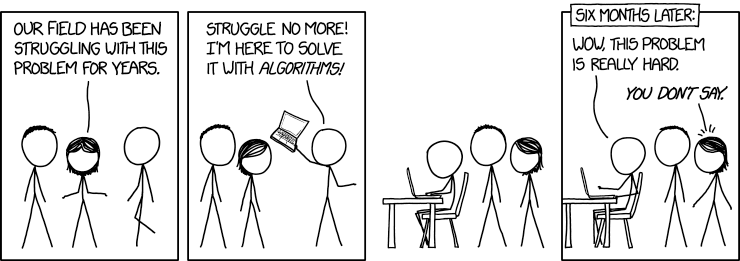
\includegraphics[width=\textwidth]{Figures/Computation/here_to_help}
\caption[Naive use of data mining and computation][Usage naïf de la fouille de données et du calcul intensif]{On naive use of data mining and intensive computation}{De l'usage naïf de la fouille de données et du calcul intensif. Source: \texttt{xkcd}}
\label{fig:computation:xkcd}
\end{figure}
%%%%%%%%%%%%%%









%----------------------------------------------------------------------------------------


%%%%%%%%%%%%%%%%%%%%%%
\subsection[Sensitivity to initial conditions][Sensibilité aux conditions initiales]{Statistical Control on Initial Conditions by Synthetic Data Generation}{Contrôle statistique pour les conditions initiales par génération de données synthétiques}


%%%%%%%%%%%%%%%%%%%%%%
\subsubsection{Context}{Contexte}


\bpar{
When evaluating data-driven models, or even more simple partially data-driven models involving simplified parametrization, an unavoidable issue is the lack of control on ``underlying system parameters'' (what is a ill-defined notion but should be seen in our sense as parameters governing system dynamics). Indeed, a statistics extracted from running the model on enough different datasets can become strongly biased by the presence of confounding in the underlying real data, as it is impossible to know if result is due to processes the model tries to translate or to a hidden structure common to all data.
}{
Lors de l'évaluation de modèle basés sur les données, ou même de modèle plus simples partiellement basés sur les données impliquant une paramétrisation simplifiée, une issue inévitable est le manque de contrôle sur les ``paramètres implicites du systèmes'' (ce qui n'est pas une notion stricte mais doit être vu dans notre sens comme les paramètres régissant la dynamique). En effet, une statistique issue d'executions du modèle sur un nombre suffisant d'executions peut toutefois rester biaisée, au sens où il est impossible de savoir si les résultats sont dus aux processus que le modèle cherche à traduire ou à une structure présente dans les données initiale. La question méthodologique fondamentale qui nous intéressera pour la suite est d'être capable d'isoler les effets propres aux processus du modèles de ceux liés à la géographie.
}



\paragraph{Rationale}{Rationelle}


\bpar{
Although simulation models of geographical systems in general and agent-based models in particular represent a fantastic opportunity to explore socio-spatial behaviours and to test a variety of scenarios for public policy, the validity of generative models is uncertain until their results are proven robust. Sensitivity analysis usually include the analysis of the effect of stochasticity on the variability of results, as well as the effects of small parameter changes. However, initial spatial conditions are usually taken for granted in geographical models, thus leaving completely unexplored the effect of spatial arrangements on the interaction of agents and of their interactions with the environment. In this part, we present a method to assess the effect of initial spatial conditions on simulation models, using a systematic generator controlled by meta-parameter to create density grids used in spatial simulation models. We show, with the example of a very classical agent-based model (Sugarscape model of ressource allocation) that the effect of space in simulation is significant, and sometimes even larger than parameters themselves. We do so using high performance computing in a very simple and straightforward open-source workflow. The benefits of this approach are various but include for example the knowledge of model behavior in an extended frame, the possibility of statistical control when regressing model outputs, or a finer exploration of model derivatives than with a direct approach.
}{
Bien que les modèles de simulation des systèmes géographiques en général et les modèles basés-agent en particulier représentent une opportunité considérable d'explorer les comportements socio-spatiaux et de tester une variété de scenarios pour les politiques publiques, la validité des modèles génératifs est incertaine tant que la robustesse des résultats n'a pas été établie. Les analyses de sensibilité incluent généralement l'analyse des effets de la stochasticité sur la variabilité des résultats, ainsi que les effets de variations locales des paramètres. Cependant, les conditions spatiales initiales sont généralement prise pour données dans les modèles géographiques, laissant ainsi totalement inexploré l'effet des motifs spatiaux sur les interactions des agents et sur leur interaction avec l'environnement. Dans cette partie, nous présentons une méthode pour établir l'effet des conditions spatiales initiales sur les modèles de simulation, utilisant un générateur systématique contrôlé par des meta-paramètres pour créer des grilles de densité utilisées dans les modèles de simulation spatiaux. Nous montrons, avec l'exemple d'un modèle agent très classique (le modèle Sugarscape d'extraction de ressources) que l'effet de l'espace dans les simulations est significatifs, et parfois plus grand que l'effet des paramètres eux-mêmes. Nous y arrivons en utilisant le calcul haute performance en un workflow très simple et open source. Les bénéfices de notre approche sont variés mais incluent par exemple la connaissance du comportement du modèle dans un contexte plus large, la possibilité de contrôle statistique pour régresser les sorties du modèles, ou une exploration plus fine des dérivées du modèle que par rapport à une approche directe.
}

\paragraph{Formalization}{Formalisation}


\bpar{
Let first give an abstract formulation of the idea. The generator is considered as an upstream model, coupled simply (outputs become inputs) with the studied downstream model. If $M_u$ is the upstream model, $M_d$ the downstream model and $\alpha$ the meta-parameters, one has the composition of the derivative along the meta-parameter
\[
\partial_{\alpha}\left[M_u \circ M_d\right] = \left(\partial_{\alpha} M_u \circ M_d \right)\cdot \partial_{\alpha} M_d
\]
It implies that the sensitivity of the downstream model to meta-parameters can be determined by studying the serial coupling and the upstream model. We gain some thematic knowledge, in the sensitivity to an implicit meta-parameter, but there is also a computational gain: the generation of controlled differentiates in the ``initial space'' would be complicated to achieve directly. The question of stochasticity in such simply coupled models causes no additional issue as $\Eb{X}=\Eb{\Eb{X|Y}}$. It naturally multiplies the number of repetition needed for convergence what is the expected behavior.
}{
Commençons par donner une formulation abstraite de l'idée, d'un point de vue du couplage de modèle. Le générateur est considéré comme un modèle amont, couplé simplement (les sorties devenant les entrées) avec le modèle aval étudié. Si $M_u$ est le model amont, $M_d$ le modèle aval et $\alpha$ les meta-paramètres, on a la composition de la dérivée le long des meta-paramètres
\[
\partial_{\alpha}\left[M_u \circ M_d\right] = \left(\partial_{\alpha} M_u \circ M_d \right)\cdot \partial_{\alpha} M_d
\]
Cela implique que la sensibilité du modèle aval aux meta-paramètres peut être déterminée en étudiant le couplage séquentiel et le modèle amont. Nous gagnons de la connaissance thématique, dans la sensibilité à un meta-paramètre implicite, mais il y a aussi un gain computationnel : la génération de différentielles contrôlées dans l'espace initial (c'est à dire tester directement la comparaison entre deux grilles proches) serait compliquer à atteindre directement. La question de la stochasticité dans de tels modèles couplés simplement ne pose pas de problème supplémentaire puisque $\Eb{X}=\Eb{\Eb{X|Y}}$. Cela multiplie naturellement le nombre de répétitions pour converger bien évidemment. Nous resterons dans l'application pratique ici à une étude de l'espace faisable de sortie et non à une étude différentielle, cette considération théorique n'influe pas à cet ordre, mais doit être gardée à l'esprit pour d'éventuelles applications plus fines.
}



\paragraph{The role of spatio-temporal path dependencies}{Role de la dépendance au chemin spatio-temporelle}


\bpar{
Spatio-temporal path dependancy is one of the main reasons making our approach relevant. Indeed, a crucial aspect of most spatio-temporal complex systems is their non-ergodicity~(\cite{pumain2012urban}) (the property that cross-sectional samples in space are not equivalent to samples in time to compute statistics such as averages), what witnesses generally strong spatio-temporal path-dependencies in their trajectories. Similar to what Gell-Mann calls \emph{frozen accidents} in any complex system~\cite{gell1995quark}, a given configuration contains clues on past bifurcations, that can have had dramatic effects on the state of the system. Temporal and cumulative effects have been considered in various geographical subfields and at various geographical scales, including transportation and urban economics, urban geography, and interregional migrations\cite{White1977},\cite{White1978}, \cite{AllenSanglier1979},\cite{Wilson1981},\cite{Pumainetal1989},\cite{AllenSanglier1981},\cite{WeidlichHaag1988},\cite{Portugali2000},\cite{Wilson2002},\cite{Batty2007},\cite{AzizAlaouiBertelle2009}. Less studied is the impact of the spatial setting on models dynamics and potential bifurcations.
}{
La dépendance au chemin spatio-temporelle est une des raisons principales rendant notre approche pertinente. En effet, un aspect crucial de la plupart des systèmes complexes spatio-temporels est leur non-ergodicité~\cite{pumain2012urban} (la propriété que les échantillons cross-sectionnels dans l'espace ne sont pas équivalent aux échantillons dans le temps pour calculer des statistiques comme la moyenne), qui témoigne généralement de forte dépendances au chemin spatio-temporelles dans les trajectoires. De manière similaire à ce que \noun{Gell-Mann} appelle \emph{frozen accidents} dans tout système complexe~\cite{gell1995quark}, une configuration donnée contient des indices sur les bifurcations passées, qui peuvent avoir eu des effets considérables sur l'état du système. Les effets temporels et cumulatifs ont été considérés dans de nombreux sous-champs géographiques et à différentes échelles géographiques, par exemple les systèmes régionaux~\cite{Wilson1981} ou l'échelle intra-urbaine~\cite{AllenSanglier1979}. L'impact de la configuration spatiale sur les dynamiques du modèle et les bifurcations spatiales a été moins étudié.
}

\bpar{
The example of transportation networks is a good illustration, as their spatial shape and hierarchy is strongly influenced by past investment decisions, technical choices, or political decisions sometimes not rational~(\cite{zembri2010new}). Some aggregated indicators will not take into account positions and trajectories of each agent (such as segregation in the Schelling model) but others, as in the case of spatial patterns of accessibility in a system of cities, fully capture the path-dependency and may therefore be highly dependent of the initial spatial configuration. It is not clear for example what shifted the economical and political capital of France from Lyon to Paris in the early Middle Age, some assumptions being the reconfiguration of trade patterns from South to North of Europe and thus an increased centrality for Paris due to its spatial position: the bifurcation induced by socio-economic and political factors took a deep significance with worldwide repercussions until today when magnified by the spatial configuration.
}{
L'exemple des réseaux de transport est une bonne illustration, car leur forme spatiale et leur hiérarchie est fortement influencée par les décisions d'investissement du passé, les choix techniques, ou des décisions politiques qui ne sont parfois pas rationelles~\cite{zembri2010new}. Certains indicateurs agrégés ne prendront pas en compte les positions et trajectoires de chaque agent (comme les inégalités totales dans le modèle Sugarscape) mais d'autres, comme dans le cas des motifs d'accessibilité spatiale dans un système de villes, capture entièrement la dépendance au chemin et peuvent ainsi être fortement dépendants à la configuration spatiale initiale. Il n'est pas clair par exemple ce qui a causé la transition de la capitale française de Lyon à Paris dans le bas Moyen-Age, certaines hypothèses étant la reconfiguration des motifs commerciaux du Sud au Nord de l'Europe et donc une centralité accrue pour Paris due à sa position spatiale, tout en gardant à l'esprit que les centralité géographique et politique ne sont pas équivalentes et entretiennent une relation complexe~\cite{guenee1968espace}. La bifurcation induite par des facteurs socio-économiques et politiques a pris une signification profonde avec des répercussions mondiales encore aujourd'hui quand elle a été concrétisée par la configuration spatiale.
}


\paragraph{Previous attempts in the literature}{Travaux existants}

\bpar{
The effect of the spatial configuration on area-based attributes of human behaviours has been largely discussed in geostatistics, meanly since the exposure of the Modifiable Areal Unit Problem (MAUP) \cite{Openshaw1984},\cite{FotheringhamWong1991}. Recently, \cite{Kwan2012} claims for a careful examination of what she coins the uncertain geographic context problem (UGCoP), that is of the spatial configuration of geographical units even if the size and delineation of the area are the same. On the contrary, the scarcity of these considerations in the geographic simulation model literature questions the generalisation of their results, as it has for instance been showed in the case of LUTI models \cite{Thomasetal2017}, of diffusion processes using ABM \cite{LeTexierCaruso2017}. 
}{
L'effet de la configuration spatiale sur les attributs agrégés à la zone des comportements humains a été largement discuté en géostatistiques, approximativement depuis l'introduction du \emph{Modifiable Areal Unit Problem} (MAUP)~\cite{Openshaw1984}. Plus récemment, \cite{Kwan2012} plaide pour un examen plus attentif de ce qui serait un \emph{Uncertain Geographic Context Problem} (UGCoP), qui est la configuration spatiale des unités géographiques même si la taille et la délimitation des zones est la même. Au contraire, le faible nombre de considérations similaires dans la littérature traitant des modèles de simulation géographiques remet en question la généralisation de leur résultats, comme cela a été montré par exemple dans le cas des modèles LUTI~\cite{Thomasetal2017}, ou des processus de diffusion étudiés par modèles basé-agents~\cite{LeTexierCaruso2017}.
}

%%%%%%%%%%%%%%%%%%%%%%
\subsubsection{Methods}{Méthodes}

\bpar{
In this section, we detail the method developed to analyse the sensitivity of simulation models to initial spatial conditions. In addition to the usual protocol, which consists of running a model $\mu$ with various values of its parameters and relating these variations of values to the variations in the simulation results, we here introduce a spatial generator, which itself is determined by parameters and produces sets of spatial initial conditions. Initial spatial conditions are clustered to represent types of spaces ex-ante (for example: moonocentric or polycentric density grids), and the sensitivity analysis of the model is now run against $\mu$ parameters as well as spatial parameters or spatial types. It allows the sensitivity analysis to produce qualitative conclusions regarding the influence of spatial distribution on the outputs of simulation models, alongside the classic variation of parameter values.
}{
Nous détaillons à présent la méthode développée pour analyser la sensibilité des modèles de simulation aux conditions spatiales initiales. S'ajoutant au protocole usuel, qui consiste à simuler un modèle $\mu$ pour différentes valeurs de ses paramètres et faire le lien entre ces variations aux variations des résultats de simulation, nous introduisons ici un générateur spatial, qui est lui-même déterminé par des paramètres et produit des ensembles de configurations spatiales initiales. Les configurations spatiales initiales sont catégorisées pour représenter des types d'espace typiques (par exemple des grilles de densité monocentriques ou polycentriques), et la sensibilité du modèle est à présent testée sur les paramètres de $\mu$ mais aussi sur les paramètres spatiaux ou les types spatiaux. Cela permet à l'analyse de sensibilité de fournir des conclusions qualitatives au regard de l'influence de la distribution spatiale sur les sorties des modèles de simulation, en parallèle des variation classiques des paramètres.
}

\paragraph{Spatial Generator}{Générateur spatial}


\bpar{
Our spatial generator applies an urban morphogenesis model developed and explored in~\ref{sec:densitygeneration}. To present it in a nutshell, grids are generated through an iterative process which adds a quantity $N$ (population) at each time step, allocating it through preferential attachment characterised by its strength of attraction $\alpha$. This first growth process is then smoothed $n$ times using a diffusion process of strength $\beta$. Grids are thus generated from the combination of the values of these four meta-parameters $\alpha$, $\beta$, $n$ and $N$, in addition to the random seed. To ease our exploration, only the distribution of density is allowed to vary rather than the size of the grid, which we fix to a 50x50 square environment of 100,000 units (cf. figure \ref{fig:spatialGen}).
}{
Le générateur spatial applique un modèle de morphogenèse urbaine développé et exploré en~\ref{sec:densitygeneration}. Pour le présenter rapidement, les grilles sont générées par un processus itératif qui ajoute une quantité de population $N$ à chaque pas de temps, l'allouant selon un attachement préférentiel caractérisé par sa force d'attraction $\alpha$. The premier processus est ensuite lissé $n$ fois par un processus de diffusion de force $\beta$. Les grilles sont donc générées aléatoirement par la combinaison des valeurs de ces quatre meta-paramètres $\alpha$, $\beta$, $n$ and $N$. Pour faciliter l'exploration, seule la distribution de densité est autorisée à varier plutôt que la taille de la grille, qui est fixée à un environnement carré 50x50 de population 100,000 unités.
}


% no schelling : ne need for this part
%\bpar{
%In order to generate density grids which correspond to empirical density distributions, we select among the generated grids using an objective function which matches the point cloud of 110 metropolitan areas in Europe described by four dimensions: their concentration index, hierarchy index, centrality index and continuity index (cf. \cite{LeNechet2015}). A stochastic exploration of a Latin Hypercube Sampling of 2000 points in the 4-dimensional space of parameters {$\alpha$, $\beta$, $n$, $N$} gives a subset of 170 interesting grids matching empirical densities, which constituted our set of different initial spatial conditions. These are further clustered into three classes of morphology: compact (e.g. Vienna), polycentric (Liege) and discontinuous (Augsburg) in order to evaluate the non-trivial effects of urban form on simulation results. We select 15 grids of each type to work with.
%}{
%Afin de générer des grilles qui correspondent à des distributions de densité empiriques,  nous en sélectionnons parmi les grilles générées en utilisant une fonction objectif qui correspond au nuage de points des 110 aires métropolitaines en Europe décrites par quatre dimensions : leur index de concentration, de hiérarchie, de centralité et de continuité (voir \cite{LeNechet2015} ; la selection ici est légèrement différente de la calibration faite en~\ref{sec:densitygeneration}, les zones cibles n'étant pas les mêmes). Une exploration stochastique par un échantillonnage Hypercube Latin de 2000 points dans l'espace à 4 dimensions des paramètres {$\alpha$, $\beta$, $n$, $N$} donne un sous-ensemble de 170 grilles pertinentes correspondant à des densités empiriques, qui constituent
%}


\paragraph{Comparing Phase Diagrams}{Comparer les diagrammes de phase}


\bpar{
In order to test for the influence of spatial initial conditions, we need a systematic method to compare phase diagrams. Indeed, we have as many phase diagrams than we have spatial grids, what makes a qualitative visual comparison not realistic. A solution is to use systematic quantitative procedures. Several potential methods could be used: for example in the case of the Schelling model, an anisotropic spatial segregation index (giving the number of clusters found and in which region in the parameter spaces they are roughly situated) would differentiate strong \emph{meta phase transitions} (phase transitions in the space of meta parameters). The use of metrics comparing spatial distributions, such as the Earth Movers Distance which is used for example in Computer Vision to compare probability distributions~\cite{rubner2000earth}, or the comparison of aggregated transition matrices of the dynamic associated to the potential described by each distribution, would also be potential tools. Map comparison methods, popular in environmental sciences, provide numeral tools to compare two dimensional fields~\cite{visser2006map}. To compare a spatial field evolving in time, elaborated methods such as Empirical Orthogonal Functions that isolates temporal from spatial variations, would be applicable in our case by taking time as a parameter dimension, but these have been shown to perform similarly to direct visual inspection when averaged over a crowdsourcing~\cite{10.1371/journal.pone.0178165}. To keep it simple and as such methodological considerations are auxiliary to the main purpose of this paper, we propose an intuitive measure corresponding to the share of between-diagrams variability relative to their internal variability. More formally, the distance is given by
}{
Afin de tester l'influence des conditions spatiales initiales, nous avons besoin d'une méthode systématique pour comparer des diagrammes de phase. En effet, nous avons autant de diagramme de phase que de grilles spatiales, ce qui rend une comparaison visuelle qualitative non réaliste. Une solution est d'utiliser des procédures quantitatives systématiques. De nombreuses méthodes pourraient potentiellement être utilisées : par exemple, des indicators anisotropes comme la donnée de clusters et leur position dans le diagramme de phase, peuvent permettre de révéler des \emph{meta-transitions de phase} (transition de phase dans l'espace des meta-paramètres. L'utilisation de métriques comparant des distributions spatiales, comme la \emph{Earth Movers Distance} qui est utilisée en viion par ordinateur pour comparer des distributions de probabilité~\cite{rubner2000earth}, ou la comparaison de matrices de transition agrégées de la dynamique associée au potentiel décrit par chaque distribution, est également possible. Les méthodes de comparaison de cartes, répandues en sciences environnementales, fournissent de nombreux outils pour comparer des champs en deux dimensions~\cite{visser2006map}. Pour comparer un champ spatial évoluant dans le temps, des méthodes élaborées comme les Fonctions Orthogonales Empiriques qui isolent les variations temporelles des variations spatiales, seraient applicables dans notre cas en prenant le temps comme une dimension de paramètre, mais celles-ci ont été montrées ayant une performance similaire à la comparaison visuelle directe lorsqu'on prend la moyenne sur un ensemble de contributions crowdsourcées~\cite{10.1371/journal.pone.0178165}. Pour rester simple et car de telles considérations méthodologiques sont auxiliaire pour le propos principal de cette partie, nous proposons une mesure intuitive correspondant à la part de la variabilité inter-diagrammes relativement à leur variabilité interne. Plus formellement, cette distance est donnée par
}

\begin{equation}\label{eq:phase-distance}
d_r\left(\alpha_1,\alpha_2\right) = 2 \cdot \frac{d(f_{\vec{\alpha_1}},f_{\vec{\alpha_2}})^2}{Var\left[f_{\vec{\alpha_1}}\right] + Var\left[f_{\vec{\alpha_2}}\right]}
\end{equation}

\bpar{
where $\alpha \mapsto \left[\vec{x} \mapsto f_{\vec{\alpha}}\left(\vec{x}\right)\right]$ is the operator giving phase diagrams with $\vec{x}$ parameters and $\vec{\alpha}$ meta-parameters, and $d$ is a distance between probability distributions that can be taken for example as basic L2 distance or the Earth's Mover Distance. For each values $\vec{\alpha_i}$, the phase diagram is seen as a random spatial field, facilitating the definition of variances and distance.
}{
où $\alpha \mapsto \left[\vec{x} \mapsto f_{\vec{\alpha}}\left(\vec{x}\right)\right]$ est l'opérateur donnant les diagrammes de phase avec $\vec{x}$ paramètres et $\vec{\alpha}$ meta-paramètres, et $d$ une distance entre distributions de probabilité qui peut être prise par exemple comme la distance L2 basique ou la \emph{Earth Movers Distance}. Pour chaque valeur $\vec{\alpha_i}$, le diagramme de phase est vue comme un champ spatial aléatoire, ce qui facilite la définition des variances et de la distance.
}




%%%%%%%%%%%%%%%%%%%%%%
\subsubsection{Results}{Résultats}


\bpar{
Sugarscape is a model of resource extraction which simulates the unequal distribution of wealth within a heterogenous population (\cite{EpsteinAxtell1996}). Agents of different vision scopes and different metabolisms harvest a self-regenerating resource available heterogeneously in the initial landscape, they settle and collect this resource, which leads some of them to survive and others to perish. The main parameters of this model are the number of agents, their minimal and maximal resource. In addition, we are interested in testing the impact of the spatial distribution of the resource in this project, using the spatial generator. The outcome of the model is measured as a phase diagram of an index of inequality for ressource distribution (Gini index). We extend the implementation with agents wealth distribution of~\cite{li2009netlogo}.
}{
Sugarscape est un modèle d'extraction de ressources qui simule la distribution inégale des richesses dans une population hétérogène~\cite{EpsteinAxtell1996}. Des agents ayant différentes portées de vision et différents métabolismes collectent une ressource qui se régénère automatiquement et disponible de manière hétérogène dans le paysage initial. Ceux-ci s'établissent et collectent la ressource, ce qui mène certains d'entre eux à survivre et d'autres à périr. Les paramètres principaux du modèle sont le nombre d'agents, leur ressources minimale et maximale. Nous nous intéressons en prime à tester l'impact de la distribution spatiale, en utilisant le générateur spatial. La sortie du modèle est mesurée comme le diagramme de phase d'un index d'inégalité pour la distribution de la ressource (index de Gini). Nous étendons l'implémentation ayant initialement une distribution de richesse des agents, donnée par~\cite{li2009netlogo}.
}


\bpar{
For the exploration, 2,500,000 simulations (1000 parameter points x 50 density grids x 50 replications) allow us to show that the model is more sensitive to space than to its other parameters, both qualitatively and quantitatively: the amplitude of variations across density grids is larger than the amplitude in each phase diagram, and the behavior of phase diagram is qualitatively different in different regions of the morphological space. More precisely, we explore a grid of a basic parameter space of the model, which three dimensions are the population of agents $P\in \left[10;510\right]$, the minimal initial agent ressource $s_{-}\in \left[10;100\right]$ and the maximal initial agent ressource $s_{+}\in \left[110;200\right]$. Each parameter is binned into 10 values, giving 1000 parameter points. We run 50 repetitions for each configuration, what yield reasonable convergence properties. The initial spatial configuration varies across 50 different grids, generated by sampling meta-parameters for the generator in a LHS. We did not use the clustered grids to test the flexibility of our framework, which is demonstrated in this case by a direct sequential coupling of the generator and the model. We mesure the distance of all 3-dimensional phase diagrams to the reference phase diagram computed on the default model setup (see Fig.~\ref{fig:sugarscape-distance} for its morphological positioning regarded generated grids), using equation~\ref{eq:phase-distance} with the L2 distance to ensure direct interpretability. Indeed, it gives in that case the average squared distance between corresponding points of the phase diagrams, relative to the average of the variance of each. Therefore, values greater than 1 will mean that inter-diagram variability is more important than intra-diagram variability.
}{
Pour l'exploration, 2,500,000 simulations (1000 points de paramètres x 50 grilles de densité x 50 réplications) nous permettent de montrer que le modèle est bien plus sensible à l'espace qu'à ses autres paramètres, à la fois quantitativement et qualitativement: l'amplitude des variations entre les grilles de densité est plus grande que l'amplitude dans chaque diagramme de phase, et le comportement de ces diagrammes de phase est qualitativement différents dans diverses régions de l'espace morphologique. Plus précisément, nous explorons une grille d'un espace de paramètre basique du modèle, dont les trois dimensions sont la population des agents $P\in \left[10;510\right]$, la ressource minimale initiale par agent $s_{-}\in \left[10;100\right]$ et la ressource initiale maximale par agent $s_{+}\in \left[110;200\right]$. Chaque paramètre est discrétisé en 10 valeurs, donnant 1000 points de paramètres. Nous procédons à 50 répétitions pour chaque configuration, ce qui donne des propriétés de convergence raisonnables. La distribution spatiale initiale varie parmi 50 grilles initiales, générée en échantillonnant les meta-paramètres du générateur dans un Hypercube Latin. Nous démontrons ainsi la flexibilité de notre cadre, par le couplage séquentiel direct du générateur avec le modèle. Nous mesurons la distance de l'ensemble des diagrammes de phase à 3 dimensions à un diagramme de phase de référence calculé sur l'initialisation du modèle par défault (voir Fig.~\ref{fig:computation:sugarscape-distance} pour sa position morphologique au regard des grilles générées), en utilisant l'équation~\ref{eq:phase-distance} avec la distance L2 pour assurer une interpretabilité directe. En effet, cela donne dans ce cas la distance au carré moyenne entre chaque points en correspondance des diagrammes, relative à la moyenne des variances de chaque. Pour cela, des valeurs plus grandes que 1 signifient que la variabilité inter-diagramme est plus importante que la variabilité intra-diagramme.
}


% summary stats
%   Min. 1st Qu.  Median    Mean 3rd Qu.    Max. 
% 0.08909 0.19790 1.52200 1.29600 2.16400 2.98100 

\bpar{
We obtain a very strong sensitivity to initial conditions, as the distribution of the relative distance to reference across grids ranges from 0.09 to 2.98 with a median of 1.52 and an average of 1.30. It means that in average, the model is more sensitive to meta-parameters than to parameters, and the relation variation can reach a factor of 3. We plot in Fig.~\ref{fig:computation:sugarscape-distance} their distribution in a morphological space. The reduced morphological space is obtained by computing 4 raw indicators of urban form, namely Moran index, average distance, rank-size slope and entropy (see~\cite{LeNechet2015} for precise definition and contextualization), and by reducing the dimension with a principal component analysis for which we keep the first two components (92\% of cumulated variance). The first measures a ``level of sprawl'' and of scattering, whereas the second measures aggregation.\footnote{We have $PC1 = 0.76\cdot distance + 0.60\cdot entropy + 0.03\cdot moran + 0.24\cdot slope$ and $PC2 = -0.26\cdot distance + 0.18\cdot entropy + 0.91\cdot moran + 0.26\cdot slope$.} We find that grids producing the highest deviations are the ones with a low level of sprawl and a high aggregation. It is confirmed by the behavior as a function of meta-parameters, as high values of $\alpha$ also yield high distance. In terms of model processes, it shows that congestion mechanisms induce rapidly higher levels of inequality.
}{
Nous obtenons une sensibilité très forte aux conditions initiales, puisque la distribution de la distance relative à la référence s'étend sur l'ensemble des grilles de 0.09 à 2.98, avec un médiane de 1.52 et une moyenne de 1.30. Cela signifie qu'en moyenne, le modèle est plus sensible aux meta-paramètres qu'aux paramètres, et que la variation relative peut atteindre jusqu'à un facteur 3. Nous montrons en Fig.~\ref{fig:computation:sugarscape-distance} leur distribution dans un espace morphologique. L'espace morphologique réduit est obtenu en calculant 4 indicateurs bruts de forme urbaine, qui sont l'index de Moran, la distance moyenne, le niveau de hiérarchie et l'entropie (voir~\cite{LeNechet2015} ainsi que la section~\ref{sec:densitygeneration} pour une définition précise et une mise en contexte), et en réduisant la dimension avec une analyse par composantes principales pour laquelle nous gardons les deux premières composantes (92\% de variance cumulée). La première mesure un ``niveau d'étalement'' et d'éclatement, tandis que la seconde mesure l'agrégation.\footnote{nous avons $PC1 = 0.76\cdot distance + 0.60\cdot entropy + 0.03\cdot moran + 0.24\cdot slope$ et $PC2 = -0.26\cdot distance + 0.18\cdot entropy + 0.91\cdot moran + 0.26\cdot slope$.} Nous trouvons que les grilles produisant les déviations les plus grandes sont celles avec un faible niveau d'étalement et une forte agrégation. Cela est confirmé par le comportement comme fonction des meta-paramètres, puisque des fortes valeurs de $\alpha$ donnent aussi une forte distance. En terme de processus du modèle, cela montre que les mécanismes de congestion induisent rapidement de plus haut niveau d'inégalités.
}

% pca of morphological space
% "","PC1","PC2","PC3","PC4"
%"distance",0.762358566609464,-0.260991693298744,0.200656405132039,0.557162237616392
%"entropy",0.601306167355116,0.181706245959277,0.0958379422351422,-0.772158547261002
%"moran",0.0311129390452153,0.912155429075071,0.30114271129527,0.276256268103684
%"slope",0.237217819823539,0.258531718397015,-0.927289147645628,0.130475642169329

%%%%%%%%%%%%%
\begin{figure}
\centering
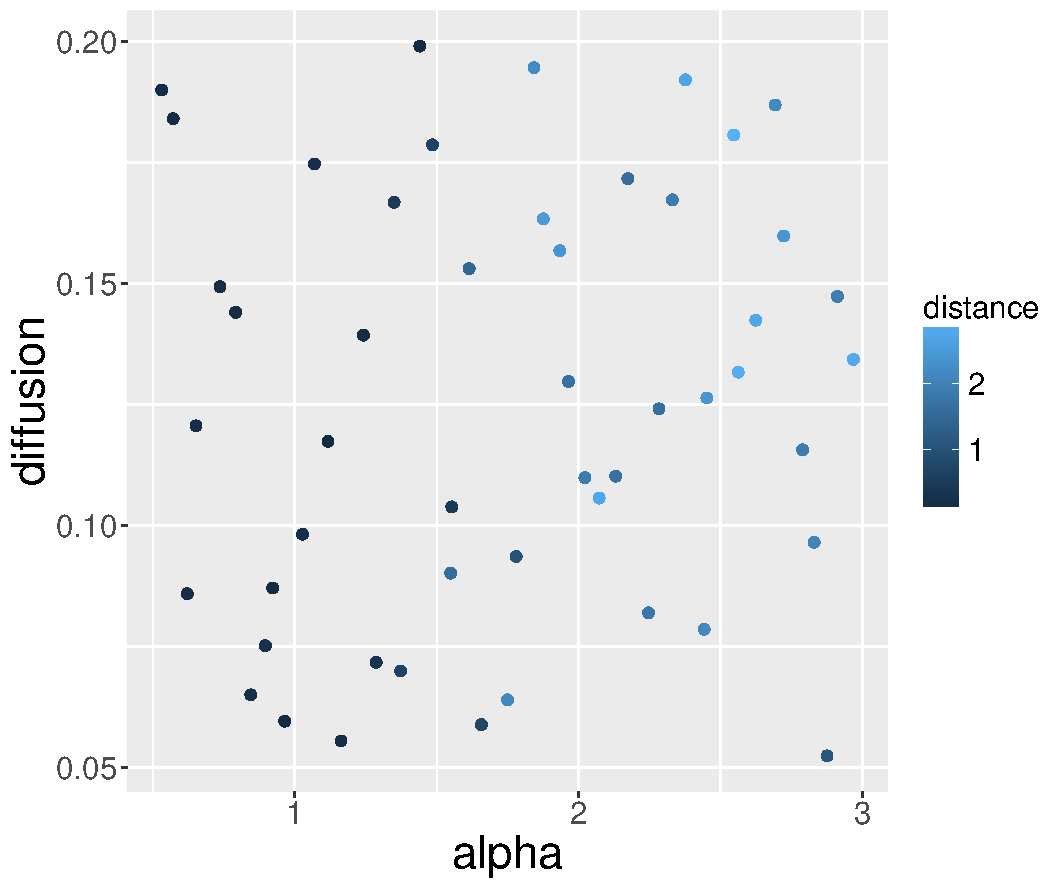
\includegraphics[width=0.49\textwidth]{Figures/Computation/relativedistance_metaparams}
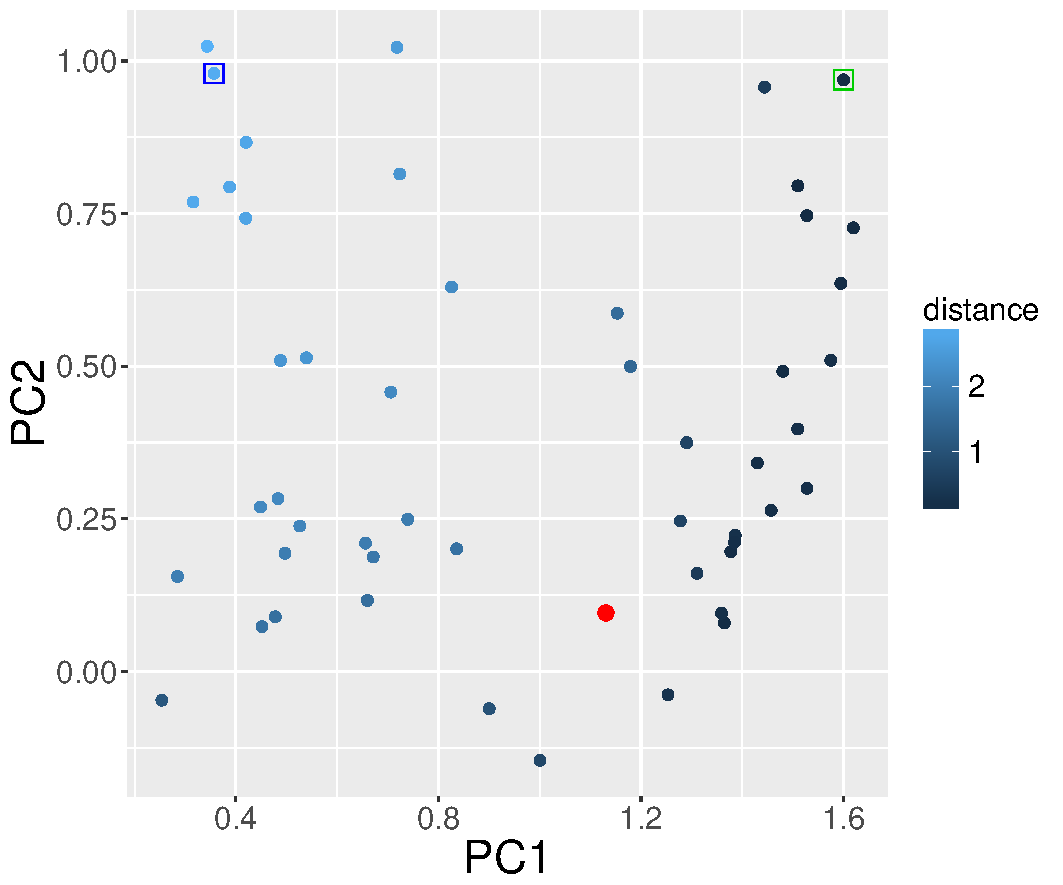
\includegraphics[width=0.49\textwidth]{Figures/Computation/relativedistance_morphspace}
\caption[Relative distances of phase diagrams to the reference][Distance des diagramme de phase à la référence]{\textbf{Relative distances of phase diagrams to the reference across grids.} (Top) Relative distance as a function of meta-parameters $\alpha$ (strength of preferential attachment) and diffusion ($\beta$, strength of diffusion process). (Bottom) Relative distance as a function of two first principal components of the morphological space (see text). Red point correspond to the reference spatial configuration. Green frame and blue frame give respectively the first and second particular phase diagrams shown in Fig.~\ref{fig:computation:sugarscape-phasediagrams}.}{\textbf{Distance relative des diagrammes de phase à la référence pour l'ensemble des grilles.} (Gauche) Distance relative comme fonction des meta-paramètres $\alpha$ (force de l'attachement préférentiel) et la diffusion ($\beta$, force du processus de diffusion). (Droite) Distance relative comme fonction des deux composantes principales de l'espace morphologique (voir texte). Le point rouge correspond à la configuration spatiale de référence. Les cadres verts et bleu donnent respectivement le premier et le second diagrammes particuliers montrés à la Fig.~\ref{fig:computation:sugarscape-phasediagrams}.}
\label{fig:computation:sugarscape-distance}
\end{figure}
%%%%%%%%%%%%%



% phase diagrams -> ok well different qualitatively
%          spAlpha spDiffsteps spDiffusion spGrowth spPopulation
% id=27 : 0.7913103    2.376837   0.1440293 157.4147 4852.746
% id=0 : 2.562398    3.753032   0.1316788 128.4632 4753.983
% maxSugar = 110


%%%%%%%%%%%%%
\begin{figure}
\centering
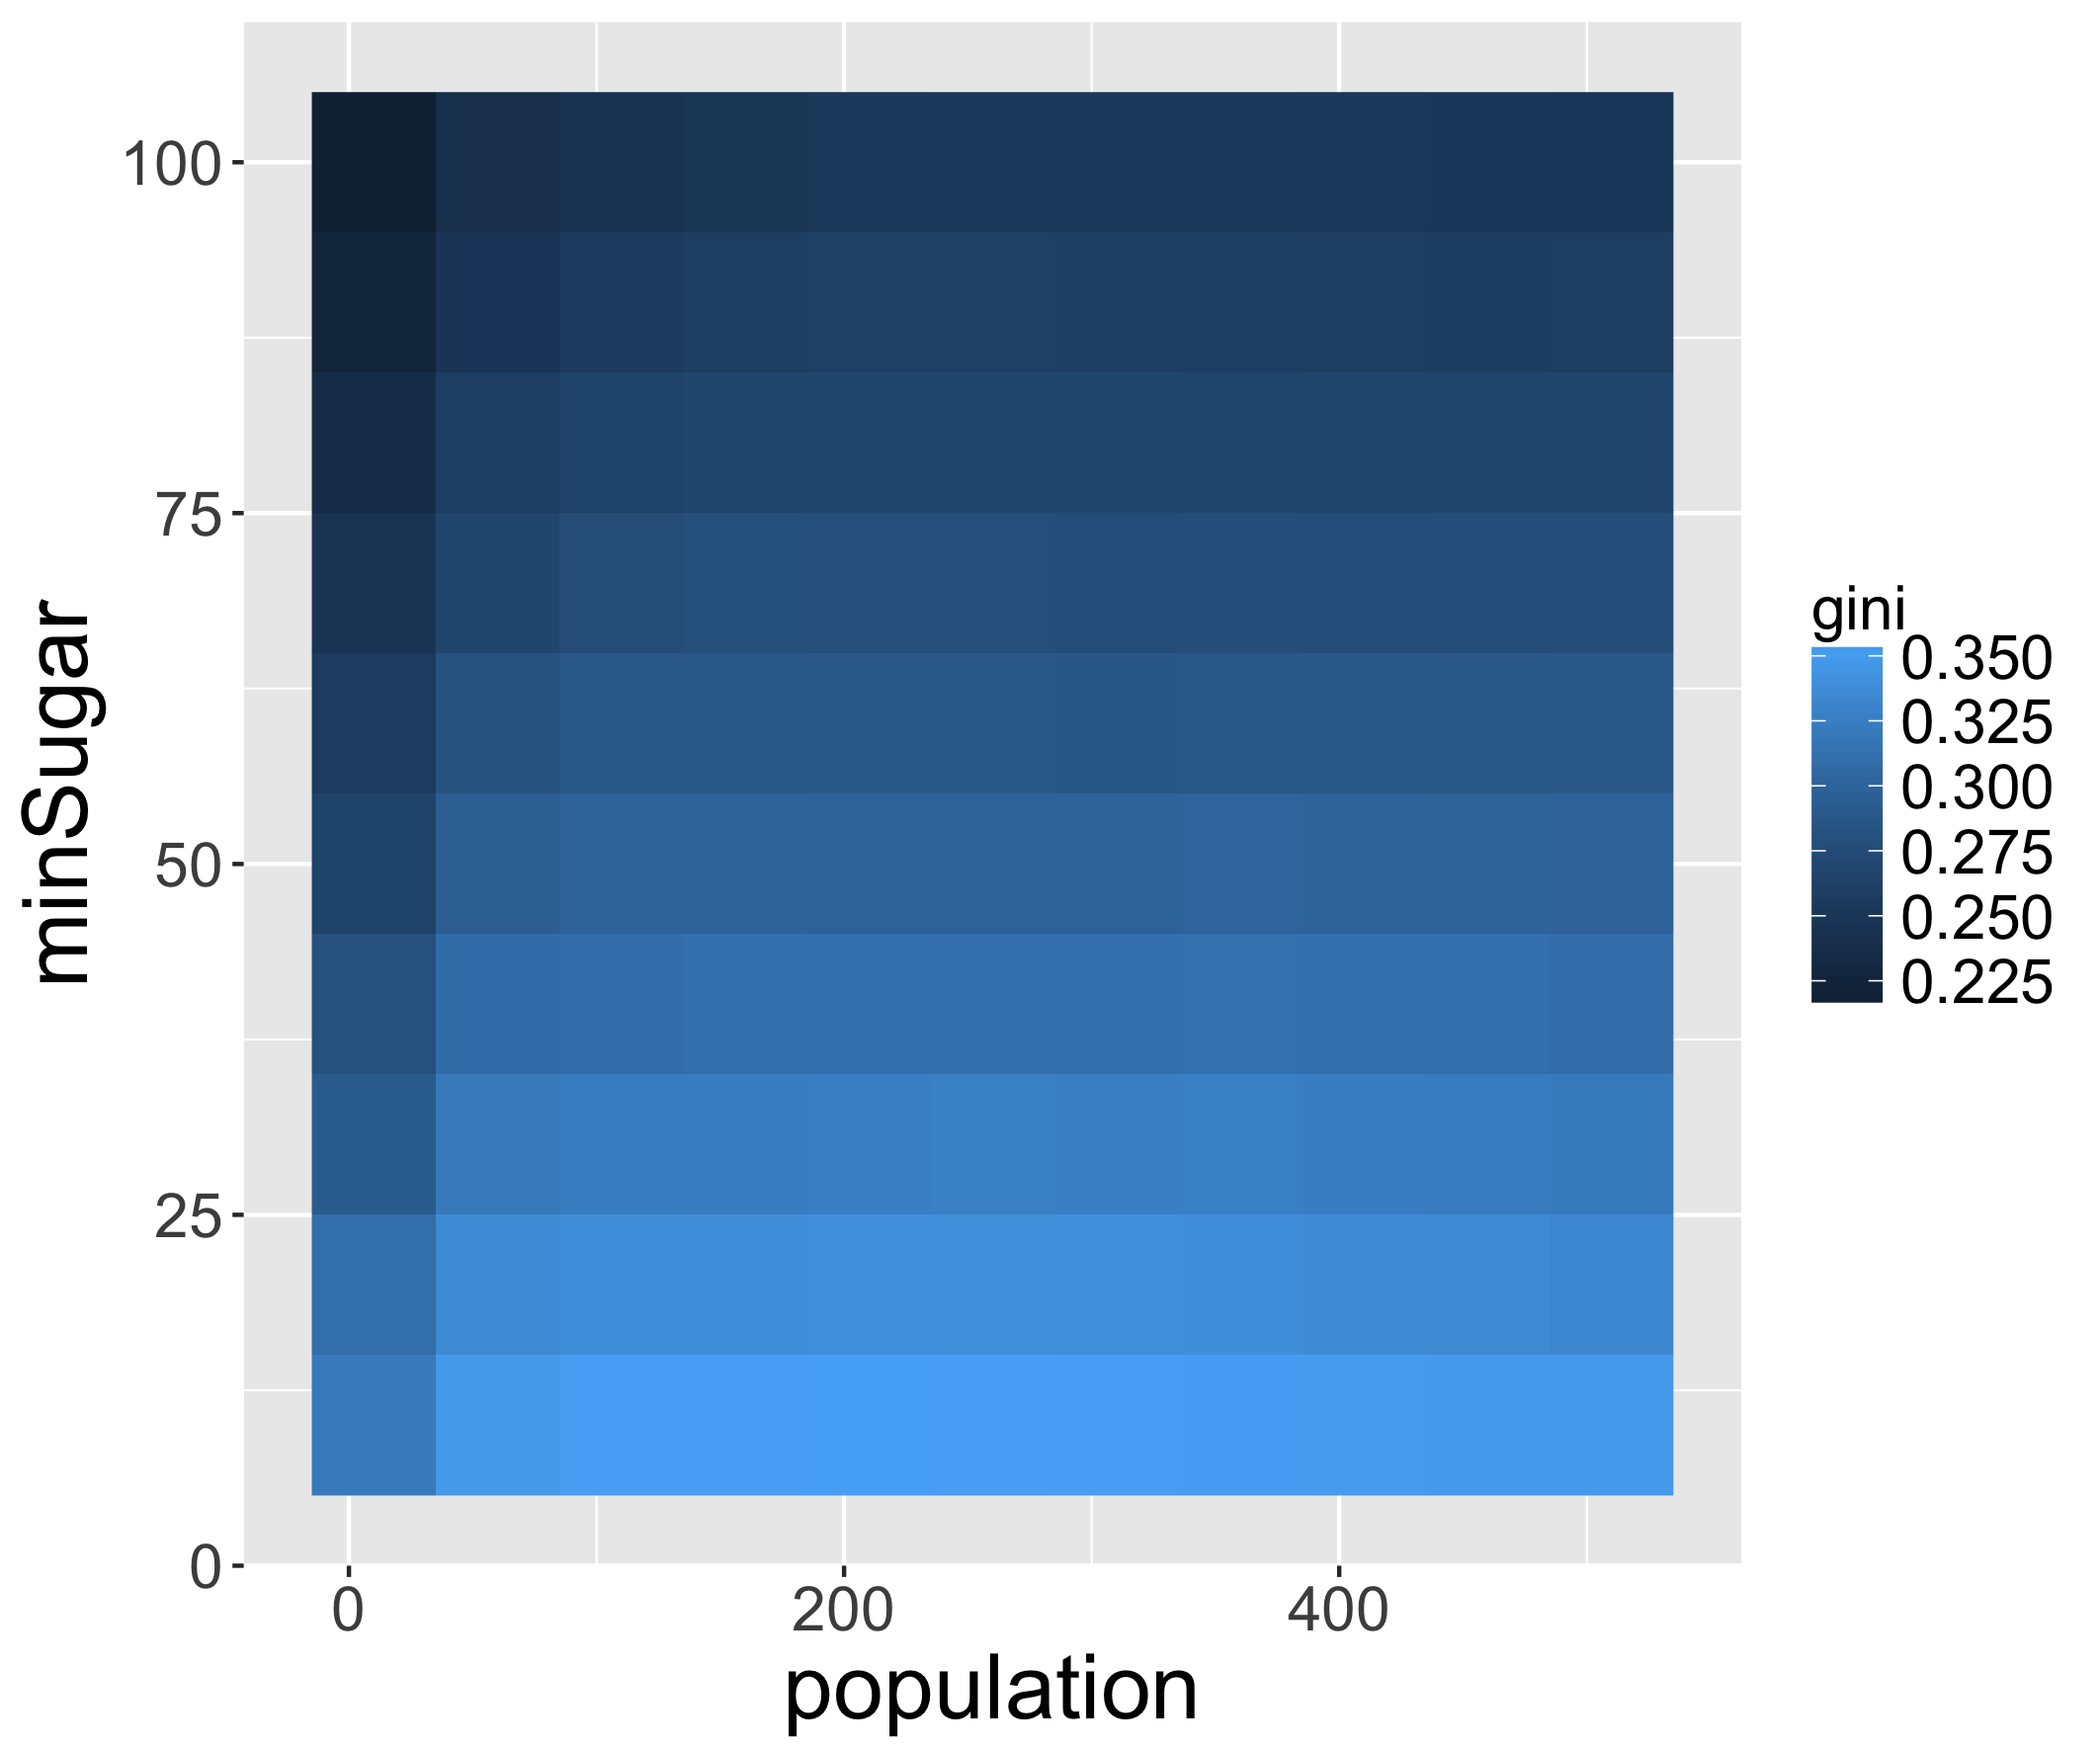
\includegraphics[width=0.49\textwidth]{Figures/Computation/phasediagram_id27_maxSugar110}
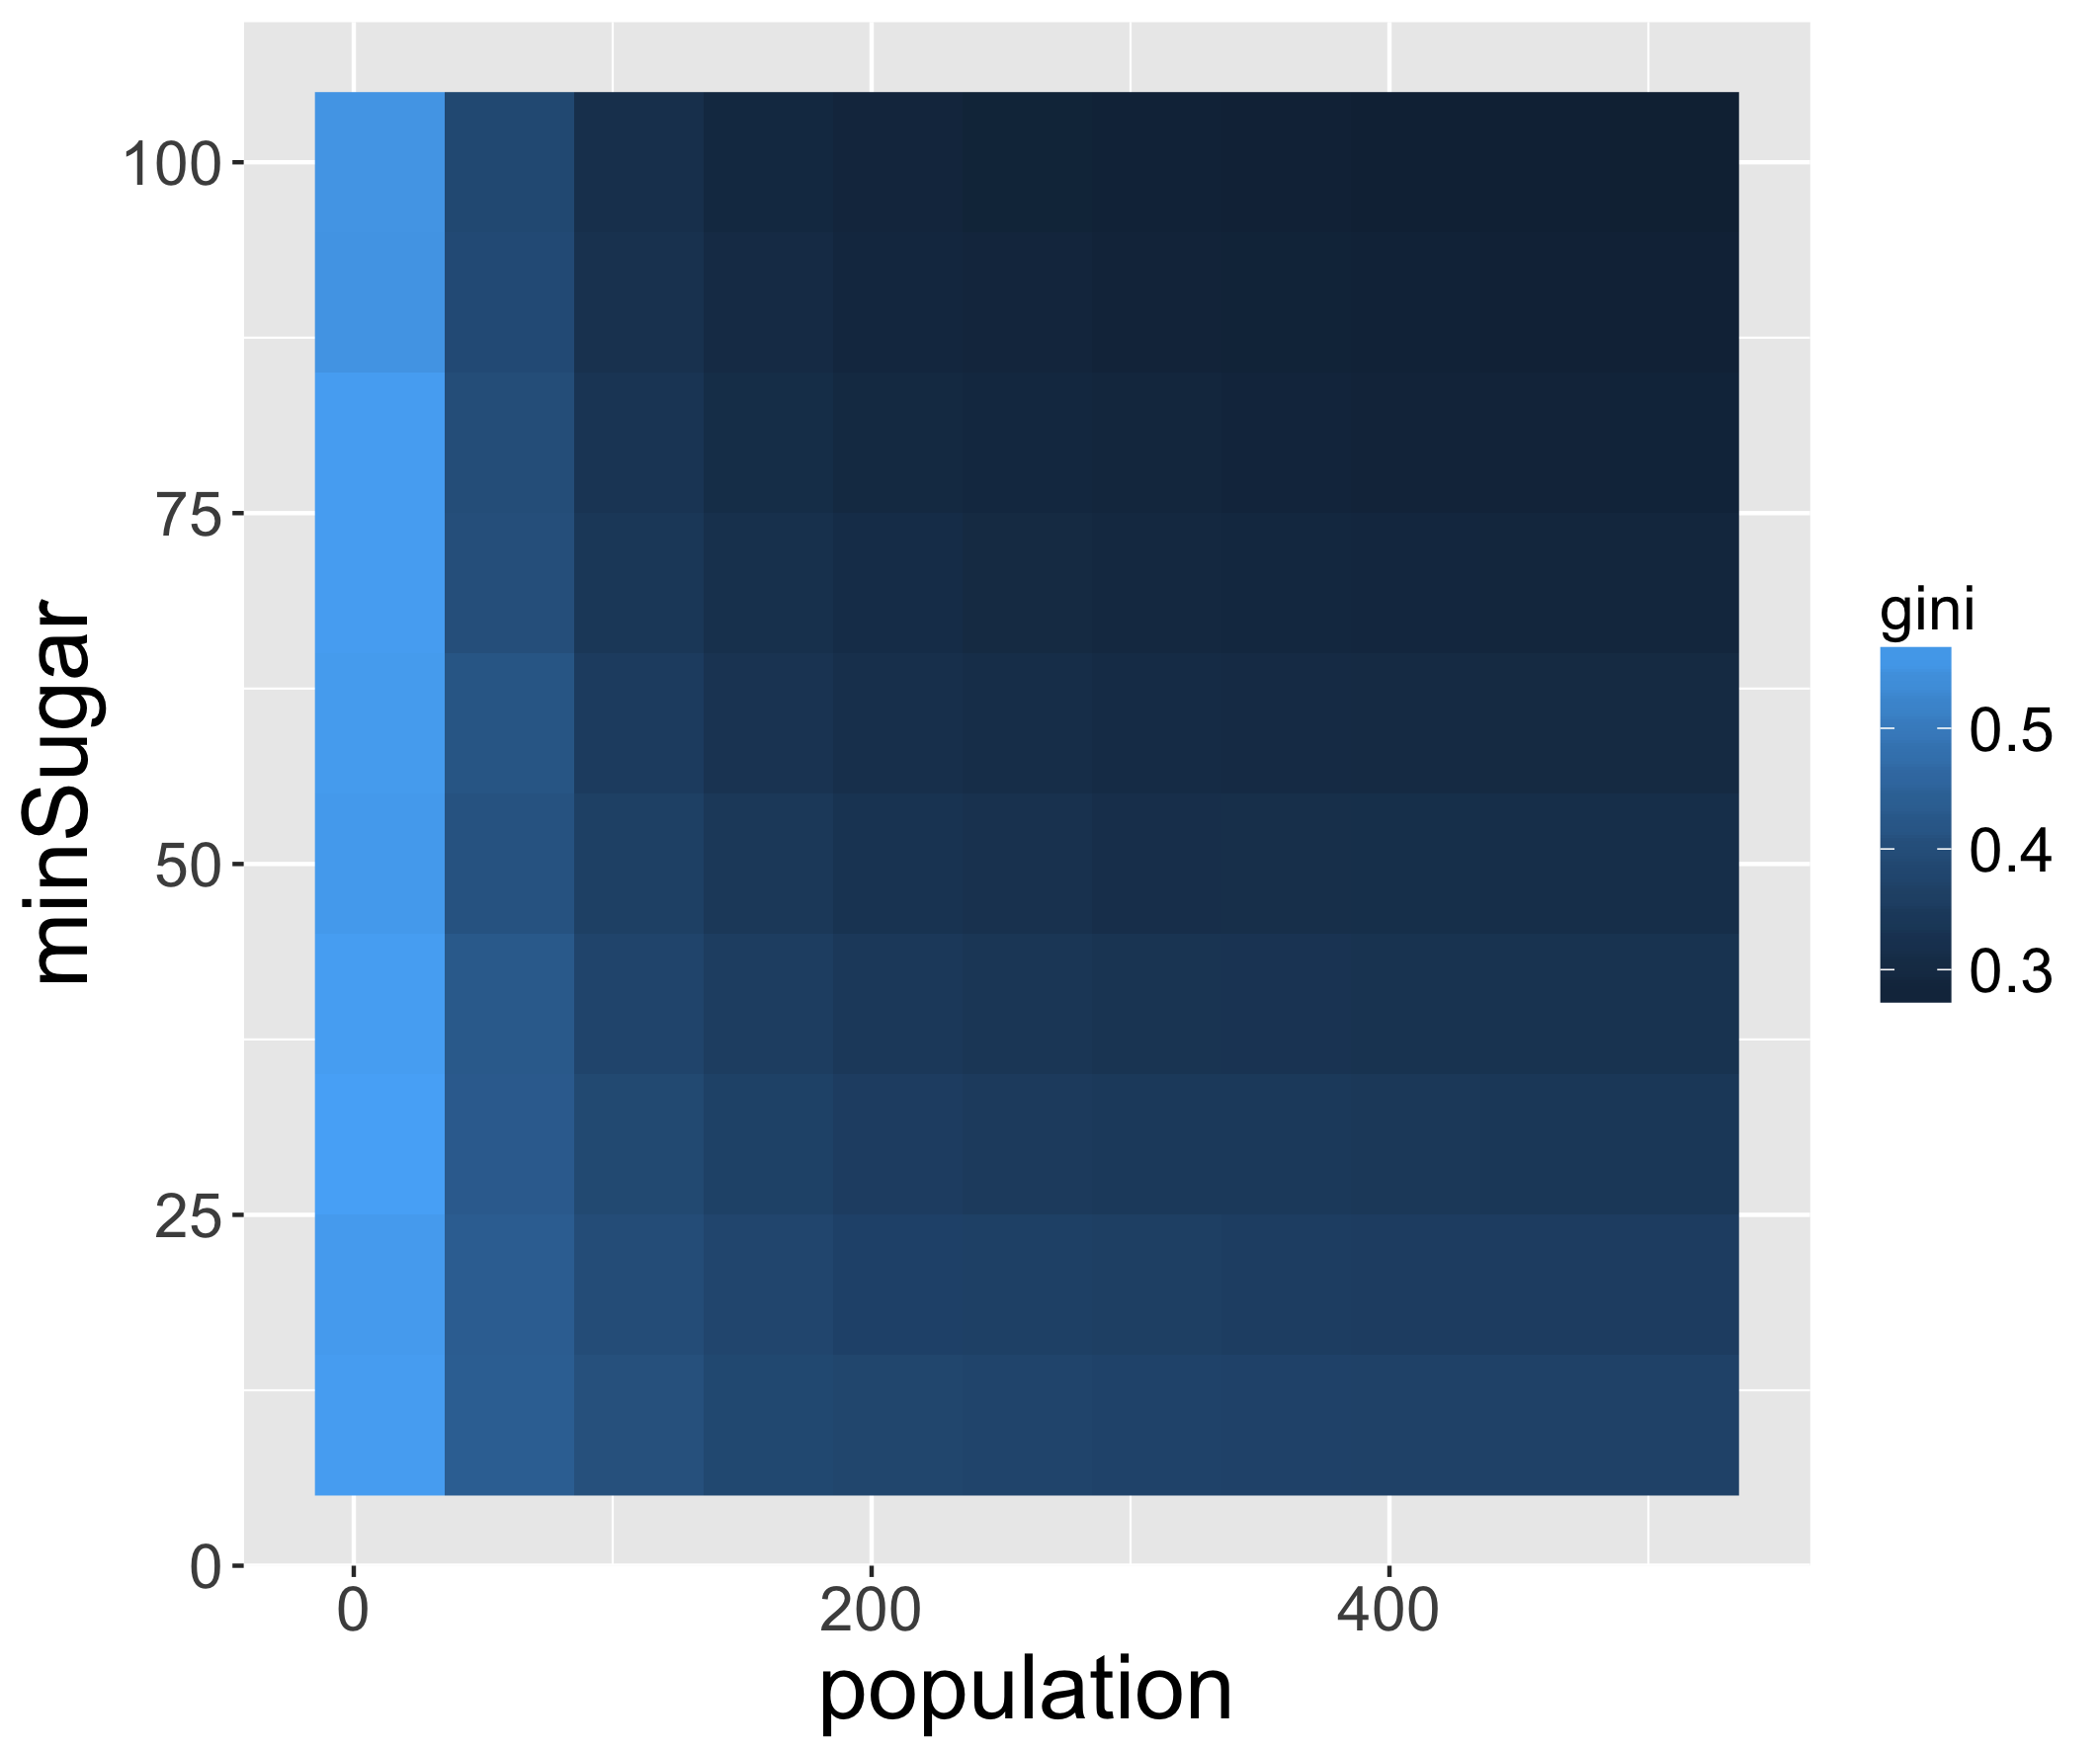
\includegraphics[width=0.49\textwidth]{Figures/Computation/phasediagram_id0_maxSugar110}
\caption[Examples of phase diagrams][Exemples de diagrammes de phase]{\textbf{Examples of phase diagrams.} We show two dimensional phase diagrams on $(P,s_-)$, both at fixed $s_+ = 110$. (Left) Green frame, obtained with $\alpha = 0.79$, $n=2$, $\beta = 0.14$, $N=157$; (Right) Blue frame, obtained with $\alpha = 2.56$, $n=3$, $\beta = 0.13$, $N=128$.}{\textbf{Exemples de diagrammes de phase.} Nous montrons deux diagrammes bi-dimensionnels sur $(P,s_-)$, obtenus à $s_+ = 110$ fixé. (Gauche) Cadre vert, obtenu avec $\alpha = 0.79$, $n=2$, $\beta = 0.14$, $N=157$ ; (Droite) Cadre bleu, obtenu avec $\alpha = 2.56$, $n=3$, $\beta = 0.13$, $N=128$.}
\label{fig:computation:sugarscape-phasediagrams}
\end{figure}
%%%%%%%%%%%%%


\bpar{
We now check the sensitivity in terms of qualitative behavior of phase diagrams. We show the phase diagrams for two very opposite morphologies in term of sprawling, but controlling for aggregation with the same $PC2$ value. These correspond to the green and blue frames in Fig.~\ref{fig:computation:sugarscape-distance}. The behaviors are rather stable for varying $s_+$, what means that the poorest agents have a determinant role in trajectories. The two examples have not only a very distant baseline inequality (the ceil of the first 0.35 is roughly the floor of the second 0.3), but their qualitative behavior is also radically opposite: the sprawled configuration gives inequalities decreasing as population decreases and decreasing as minimal wealth increases, whereas the concentrated one gives inequalities strongly increasing as population decreases and also decreasing with minimal wealth but significantly only for large population values. The process is thus completely inverted, what would have significant impacts if one tried to schematize policies from this model. This second example confirms thus the importance of sensitivity of simulation models to the initial spatial conditions.
}{
Nous contrôlons à présent la sensibilité en terme de comportement qualitatif des diagrammes de phase. Nous montrons en Fig.~\ref{fig:computation:sugarscape-phasediagrams} les diagrammes pour deux morphologies très opposées en terme d'étalement, mais en contrôlant l'agrégation par la même valeur de $PC2$. Ceux-ci correspondent au cadres vert et bleu en Fig.~\ref{fig:computation:sugarscape-distance}. Les comportements sont relativement stables pour $s_+$ variant, ce qui signifie que les agents les plus pauvres ont un rôle déterminant dans les trajectoires. Les deux examples ont non seulement une inégalité de base très distance (le plafond du premier 0.35 est environ le plancher du second 0.3), mais leur comportement qualitatif est également radicalement opposé: la configuration étalée donne des inégalité qui décroissent quand la population décroît et qui décroissent quand la richesse minimale augmente, tandis que la concentrée donne des inégalités augmentant fortement quand la population décroît et aussi décroissantes avec la richesse minimale mais significativement seulement pour des grandes valeurs de population. Le processus est ainsi complètement inversé, ce qui aurait un impact déterminant si l'on essayait de schématiser des politiques à partir du modèle. Cet exemple confirme ainsi l'importance de la sensibilité des modèles de simulation aux conditions spatiales initiales.
}















%%%%%%%%%%%%%%%%%%%%
\subsection{Link between modeling and Open Science}{Lien entre modélisation et Science Ouverte}



\bpar{
The last methodological point which we need to emphasis is the relation between the workflow we introduce and model exploration workflows. The ideas of multi-modeling and extensive model exploration are nothing from new as Openshaw already advocated for ``model-crunching'' in~\cite{openshaw1983data}, but their effective use only begins to emerge thanks to the apparition of new methods and tools together with an explosion of computation capabilities: \cite{cottineau2016back} claims for a renewed approach on multi-modeling. Coupling models as we do answers to similar questions. In that stream of research, the model exploration platform OpenMole~\cite{reuillon2013openmole} allows to embed any model as a blackbox, write modulable exploration workflow using advanced methodologies such as genetic algorithms and distribute transparently the computation on large scale computation infrastructures such as clusters or computation grids. In our case, the workflow tool is a powerful way to embed both the sensitivity analysis and the meta-sensitivity analysis, and allow to couple any generator with any model in a straightforward way as soon as the model can take its spatial configuration as input or from an input file.
}{
Enfin, il est important de souligner brièvement les liens entre pratiques de modélisation et science ouverte, comme le lien entre reproductibilité et science ouverte souligné à la fin de~\ref{sec:reproducibility}. En fait, la Science Ouverte est composée d'un ensemble de pratiques sur différents points, d'où sa ventilation logique dans nos positionnements. Pour illustrer les enjeux, nous proposons de décrire l'exemple des workflows d'exploration de modèle comme une méthode de meta-analyse de sensibilité, c'est à dire un aspect de la méthodologie appliquée ci-dessus. Les idées de multi-modélisation et d'exploration intensive de modèle sont tout sauf nouvelles puisque \noun{Openshaw} défendait déjà le ``model-crunching'' dans~\cite{openshaw1983data}, mais leur utilisation effective commence seulement à émerger grâce à l'apparition de nouvelles méthodes et outils en même temps qu'une explosion des capacités de calcul : \cite{cottineau2016back} plaide pour une approche renouvelée de la multi-modélisation. Le couplage de modèles comme nous faisons répond à des questions similaires. Dans cette lignée de recherche, la plateforme d'exploration de modèle OpenMole~\cite{reuillon2013openmole} permet d'embarquer n'importe quel modèle comme une boîte noire, d'écrire des workflow d'exploration modulables qui utilisent des méthodologies d'exploration avancées comme des algorithmes génétiques, et de distribuer de manière transparente les calculs sur des infrastructures de calcul à grande échelle comme des clusters ou grilles de calcul. Dans le cas précédent, l'outil du workflow est un outil puissant pour intégrer à la fois l'analyse de sensibilité et la meta-analyse de sensibilité, et permet de couplet n'importe quel générateur avec n'importe quel modèle de façon très directe tant que le modèle peut prendre sa configuration spatiale comme entrée ou dans un fichier d'entrée. D'autre part, une idée des workflow est de favoriser des constructions ouvertes et collaboratives, puisque le ``marketplace'' d'OpenMole, directement intégré au logiciel, permet de bénéficier directement des exemples qui auront été partagés sur le dépôt collaboratif. Cela ressemble aux plateformes de partage de modèles, qui sont nombreuses pour les modèles agents par exemple, mais dans un esprit encore plus modulaire et participatif. Ainsi, certains choix épistémologiques et méthodologiques au regard de la modélisation impliquent directement un positionnement au regard de la science ouverte : la multi-modélisation et les familles de modèles, qui vont de pair avec le couplage de modèle hétérogènes et multi-échelles, ne peuvent guère être viables sans des pratiques d'ouverture, de partage et de construction collaborative des modèle, comme le rappelle~\cite{banos2013pour}.
}







\stars










%
% 3.3 Epistemological positioning



%----------------------------------------------------------------------------------------


\newpage



\section{Epistemological Positioning}{Positionnement Epistémologique}\label{sec:epistemology}

%----------------------------------------------------------------------------------------



%%%%%%%%%%%%%%%%%%%%%%
\subsection{Cognitive Approach and Perspectivism}{Approche cognitive et Perspectivisme}



\bpar{
Our epistemological positioning relies on a cognitive approach to science, given by Giere in~\cite{giere2010explaining}. The approach focuses on the role of cognitive agents as carriers and producers of knowledge. It has been shown to be operational by \cite{giere2010agent} that studies an agent-based model of science. These ideas converge with Chavalarias' Nobel Game~\cite{chavalarias2016s} that tests through a stylized model the balance between exploration and falsification in the collective scientific enterprise. This epistemological positioning has been presented by Giere as \emph{scientific perspectivism}~\cite{giere2010scientific}, which main feature is to consider any scientific entreprise as a \emph{perspective} in which \emph{agents} use \emph{media} (models) to represent something with a certain purpose. To make it more concrete, we can position it within Hacking's ``check-list'' of constructivism~\cite{hacking1999social}, a practical tool to position an epistemological position within a simplified three dimensional space which dimensions are different aspects on which realist approaches and constructivist approach generally diverge: first the contingency (path-dependency of the knowledge construction process) is necessary in the pluralist perspectivist approach, secondly the ``degree of constructivism'' is quite high because agents produce knowledge, and finally the stability of theories depends on the complex interaction between the agents and their perspectives. It was presented for these reasons as an intermediate and alternative way between absolute realism and skeptical constructivism~\cite{brown2009models}. The \emph{perspective} plays a central role in the framework.
}{
Notre positionnement épistémologique se fonde sur une approche cognitive de la science, introduite par \noun{Giere} dans~\cite{giere2010explaining}. L'approche se concentre sur le rôle des agents cognitifs comme porteurs et producteurs de la connaissance. Son opérationalité a été montrée par \cite{giere2010agent} qui étudie un modèle basé-agent de la science. Ces idées convergent avec le jeu Nobel de \noun{Chavalarias}~\cite{chavalarias2016s} qui teste de manière stylisée l'équilibre entre exploration et falsification \comment[AB]{est-ce vraiment le bon couple ? A vérifier} dans l'entreprise scientifique collective. Ce positionnement épistémologique a été présenté par \noun{Giere} comme \emph{perspectivisme scientifique}~\cite{giere2010scientific}, dont la caractéristique principale est de considérer toute entreprise scientifique comme une \emph{perspective} dans laquelle des \emph{agents} utilisent des \emph{media} (modèles) pour représenter quelque chose dans un certain but. Pour concrétiser, nous pouvons le positionner sur la \emph{check-list} du constructivisme de \noun{Hacking}~\cite{hacking1999social}, un outil pratique pour positionner une position épistémologique dans un espace simplifié à trois dimensions dans lequel les dimensions sont différents aspects sur lesquels les approches réalistes et constructivistes généralement divergent : d'abord la contingence (dépendance au chemin du processus de construction de connaissances) est nécessaire l'approche perspectiviste qui est pluraliste, deuxièmement le ``degré de constructivisme'' est assez haut car les agents produisent la connaissance, et enfin la stabilité des théories dépend des interactions complexes entre les agents et leur perspectives \comment[AB]{reprendre plus clairement}. Cela a pour ces raisons été présenté comme un chemin intermédiaire et alternatif entre le réalisme absolu et le constructivisme sceptique~\cite{brown2009models}. la notion de \emph{perspective} jouera un rôle fondamental dans le cadre développé en~\ref{sec:knowledgeframework}.
}

Cette approche mettant l'emphase sur l'auto-organisation, nous la voyons totalement compatible avec une vision anarchiste de la science comme défendue par \noun{Feyerabend}~\cite{feyerabend1993against}. Celui-ci émet des doutes sur l'intérêt de l'anarchisme politique mais introduit l'\emph{anarchisme scientifique}, qu'il ne faut pas comprendre comme un refus total de toute méthode ``objective'', mais d'une autorité et légitimité artificielle que certaines méthodes ou courants scientifique pourraient vouloir prendre. Il démontre par une analyse précise des travaux de Galilée que la plupart de ses résultats étaient basés sur des croyances et que la plupart n'étaient pas accessibles avec les outils et méthodes de l'époque, et postule qu'il devrait en être de même pour certains travaux contemporains. Il n'y a donc pas de \emph{perspective} objectivement plus légitimes que d'autres dans la mesure de leurs validation par des faits et des pairs - et même dans ces cas la légitimité doit pouvoir être discutée, car la remise en question est un fondement de la connaissance. Cela correspond exactement à la pluralité des perspectives que nous défendons. L'auto-organisation et l'émergence des connaissance nécessitent un certain anarchisme pour échapper aux préconceptions cadrant par le haut \comment[AB]{a revoir}. En effet, les positions anarchistes ont trouvé un écho très cohérent dans les différents courants de la complexité, de la cybernétique à l'auto-organisation au cours du 20ème siècle~\cite{duda2013cybernetics}. Notre cadre de connaissances développé en~\ref{sec:knowledgeframework} illustre cette émergence de la connaissance. De plus, notre volonté de réflexivité et de donner à notre travail des pistes de lecture diverses au delà de la linéarité (voir \ref{app:reflexivity}), illustre l'application de ces principes. Les recommandations méthodologiques et les positionnements donnés précédemment dans ce chapitre pourraient sonner comme totalitaires s'ils étaient assénés de manière sèche sans contexte, mais ceux-ci sont en fait tout le contraire puisqu'ils découlent d'un dynamique récente de science ouverte qui a bien émergé par le bas, conséquence en partie de l'ouverture et de la pluralité.

% concerning the cs framework : what is deconstructivism ; position our approach in regard ? Feyerabend as a confirmation ? - eventually search for that and develop later.






%%%%%%%%%%%%%%%%%%%%%%
\subsection{From Life to Culture}{De la Vie à la Culture}

Le parallèle entre les systèmes sociaux et les systèmes biologiques est souvent fait, parfois de manière plus qu'imagée comme par exemple pour la théorie du \emph{Scaling} de \noun{West} qui applique des équations de croissance similaires à partir des lois d'échelle, avec des conclusions inverses tout de même concernant la relation entre taille et rythme de vie~\cite{bettencourt2007growth}. Les relations d'échelle ne tiennent plus lorsqu'on essaye de les appliquer à une fourmi seule, et il faut alors l'appliquer à la fourmilière entière qui est alors l'organisme en question. En ajoutant la propriété de cognition, on confirme qu'il s'agit du niveau pertinent, puisque celle-ci possède des propriétés cognitives avancées, comme la résolution de problèmes d'optimisation spatiaux, ou la réponse rapide à une perturbation extérieure. Les organisations sociales humaines, les villes, peuvent-elles être vues comme des organismes ? \noun{Banos} file dans~\cite{banos2013pour} la métaphore de la \emph{fourmilière urbaine} mais rappelle que le parallèle s'arrête assez vite. Nous allons voir cependant dans quelle mesure certains concepts de l'épistémologie de la biologie peuvent être utiles pour comprendre les systèmes sociaux que nous nous proposons d'étudier. Nous nous basons sur la contribution fondamentale de \noun{Monod} dans~\cite{monod1970hasard}, qui tente de développer les principes épistémologiques cruciaux pour l'étude du vivant. Ainsi, les organismes vivants répondent à trois propriétés essentielles qui permettent des les différencier d'autres systèmes : (i) la téléonomie, c'est à dire qu'il s'agit ``d'objets doués d'un projet'', projet qui se reflète dans leur structure et dans celles des artefacts qu'ils produisent\footnote{à ne pas confondre avec la téléologie, propres aux animismes, qui consiste à prêter un projet ou un sens à l'univers} ; (ii) l'importance des processus morphogénétiques dans leur constitution (voir~\ref{sec:interdiscmorphogenesis}) ; (iii) la propriété de reproduction invariante de l'information définissant leur structure. \noun{Monod} esquisse de plus en conclusion des pistes pour une théorie de l'évolution culturelle. La téléonomie est essentielle dans les structures sociales, puisque toute organisation essaye de satisfaire un ensemble d'objectifs, même si en général elle n'y parviendra pas et que ceux-ci co-évolueront avec l'organisation. Un aspect divergent est cette notion de multi-objectif qui est typique des systèmes complexes socio-techniques. Ensuite, nous postulons que la notion de morphogenèse est un outil essentiel pour comprendre ces systèmes, avec une définition très proche de celle utilisée en biologie. Un travail approfondi pour donner cette définition est fait en~\ref{sec:interdiscmorphogenesis}, que nous résumerons en l'existence de processus relativement autonomes guidant la croissance du système et impliquant des relations causales circulaires entre forme et fonction qui témoignent d'une architecture émergente. Pour des systèmes sociaux, isoler le système est plus difficile et la notion de frontière sera moins stricte que pour un système biologique, mais on retrouvera bien ce lien entre forme et fonction, comme par exemple la structure d'une organisation ayant un impact sur ses fonctionnalités. Enfin, la reproduction de l'information est au coeur de l'évolution culturelle, par la transmission de la culture et la \emph{mémétique}, la différence étant que le rapport d'échelle de temps entre la fréquence de transmission et les processus de croisement et de mutation ou d'autres processus non mémétiques de production culturelle est très faible, alors qu'elle est de plusieurs ordres de magnitude en biologie. \cite{2017arXiv170305917G} propose un modèle de réseau auto-catalytique pour la cognition, qui expliquerait l'apparition de l'évolution culturelle par des processus analogues à ceux s'étant produit à l'apparition de la vie, c'est à dire une transition permettant au molécules de s'auto-entretenir et s'auto-reproduire, les représentations mentales faisant office de molécules. Cet exemple montre bien que le parallèle n'est pas toujours absurde. Mais si les processus à l'origine sont analogues, la nature de l'évolution est bien différente par la suite, comme le montre \cite{vanderLeeuw2009}, les critères darwiniens d'évolution n'étant pas suffisant pour expliquer l'évolution de nos sociétés organisées. Il s'agit d'un degré de complexité supérieur\comment[AB]{vraiment ? Eléments factuels à avancer} et le rôle des flux d'information est crucial (voir le rôle de la complexité informationnelle dans la sous-section suivante). Enfin, l'un des points sur lequel il s'agit d'être attentif, est la plus grande difficulté de définir les niveaux d'émergence pour les systèmes sociaux : \cite{roth2009reconstruction} souligne le risque de tomber dans des cul-de-sac ontologiques car les niveaux ont été mal définis. Il soutient qu'il faut d'une manière générale penser au-delà de la seule dichotomie micro-macro qui est utilisée pour caricaturer les notions d'émergence faible, mais que les ontologies doivent souvent être multi-niveaux et impliquant de multiples niveaux intermédiaires.

\comment{\cite{Mesoudi25072017}}




%----------------------------------------------------------------------------------------

\subsection{Nature of Complexity and Knowledge Production}{Nature de la Complexité et Production de Connaissances}

Un aspect de la production de connaissance sur des Systèmes Complexes, auquel nous nous heurtons plusieurs fois ici (voir chapitre~\ref{ch:theory}), et qui semble être récurrent voire inévitable, est un certain niveau de réflexivité (et qui serait inhérent aux systèmes complexes en comparaison aux systèmes simples, comme nous le développerons plus loin). Nous entendons par là à la fois une réflexivité pratique, c'est à dire la nécessité d'élever le niveau d'abstraction, comme le besoin de reconstruire de manière endogène les disciplines dans lesquelles une réflexion cherche à se positionner comme proposé en \ref{sec:quantepistemo}, ou de réfléchir à la nature épistémologique de la modélisation lors de l'élaboration d'un modèle comme en \ref{sec:csframework}, mais également une réflexivité théorique en le sens que les appareils théoriques ou les concepts produits peuvent s'appliquer de manière récursive à eux-mêmes. Cette constatation pratique fait echo à des débats épistémologiques anciens questionnant la possibilité d'une connaissance objective de l'univers qui serait indépendante de notre structure cognitive, ou bien la nécessité d'une ``rationalité évolutive'' impliquant que notre système cognitif, produit de l'évolution, reflète les processus complexes ayant conduit à son émergence, et que toute structure de connaissance sera par conséquent réflexive\footnote{Nous remercions D. Pumain d'avoir pointé cette vue alternative du problème que nous allons développer par la suite}. Nous ne prétendons pas ici apporter une réponse à une question aussi vaste et vague telle quelle, mais proposons un lien potentiel entre cette réflexivité et la nature de la complexité.


\paragraph{Complexity and Complexities}{Complexité et Complexités}

Ce qui est entendu par complexité d'un système mène souvent à des malentendus car celle-ci peut être qualifiée selon différentes dimensions et visions. Nous distinguons d'une part la complexité au sens d'émergence faible et d'autonomie entre les différents niveaux d'un système, et sur laquelle différentes positions peuvent être développées comme dans \cite{deffuant2015visions}. Nous ne rentrerons pas dans une granularité plus fine, la vision de la complexité sociale donnant encore plus de fil à retordre au démon de Laplace, peut être par exemple comprise par une émergence plus forte, la nature des systèmes ne jouant pas de rôle dans notre reflexion.\comment[AB]{je vois l’idée mais c’est loin d’être clair ==> à clarifier} D'autre part, nous distinguons deux autres ``types'' de complexité, la complexité computationnelle et la complexité informationnelle, qui peuvent être vues comme des mesures de complexité, mais qui ne sont pas directement équivalentes à l'émergence, puisqu'il n'existe pas de lien systématique entre les trois. On peut par exemple imaginer utiliser un modèle de simulation, pour lequel les interactions entre agents élémentaires se traduisent par un message codé au niveau supérieur: il est alors possible en exploitant les degré de liberté de minimiser la quantité d'information contenue dans le message. Les différentes langues demandent des efforts cognitifs différents et compressent différemment l'information, ayant différents niveau de complexité mesurables~\cite{febres2013complexity}. De même, des artefacts architecturaux sont le résultat d'un processus d'évolution naturelle puis culturelle et peuvent témoigner plus ou moins de cette trajectoire. D'autres caractérisations conceptuelles ou opérationnelles de la complexité existent, et il est clair que la communauté scientifique n'a pas convergé sur une définition unique~\cite{chu2008criteria}\footnote{Dans une approche en un sens réflexive, \cite{chu2008criteria} propose de continuer d'explorer les différentes approches existantes, comme des proxys de la complexité dans le cas d'un essentialisme, ou comme des notions à part entière. La complexité devrait émerger d'elle même de l'interaction entre ces différentes approches étudiant la complexité (d'où la réflexivité).}. Nous proposons de nous concentrer sur ces trois concepts en particulier, pour lesquels les relations ne sont déjà pas évidentes. En effet, les liens entre ces trois types de complexité ne sont pas systématiques, et dépendent du type de système. Des liens épistémologiques peuvent néanmoins être introduits. Nous traitons ceux entre émergence et les deux autre complexités, étant donné que le lien entre complexité computationnelle et complexité informationnelle est assez bien compris et relève de problématiques de compression de l'information et de traitement du signal, ou encore de cryptographie.

\comment[JR]{Gell-mann : effective complexity : AIC of CAS observing an other CAS : prelude to perspectivism ? check link between information and Kolmogorov complexity - add Kolmogorov complexity in computational complexity.}


\paragraph{Computational Complexity}{Complexité computationnelle et émergence}



Différents indices suggèrent une certaine nécessité de complexité computationnelle pour avoir émergence dans des systèmes complexes, tandis que réciproquement un certain nombre de systèmes complexes adaptatifs sont dotés de capacités de calcul élevées. 

Le ``paradoxe'' du chat de Schrödinger n'en est un que sous une perspective réductionniste, c'est à dire si l'on suppose que la superposition d'états peut se propager à travers les niveaux successifs et qu'il n'y aurait pas émergence, au sens de constitution d'un niveau supérieur autonome.\comment[AB]{trop elliptique là aussi : on ne voit pas clairement le lien avec el gato. Sois plus précis} Cette vision intuitive a récemment été démontrée rigoureusement par \cite{2014arXiv1403.7686B} qui prouve que l'acceptation de $\mathbf{P}\neq\mathbf{NP}$ implique une séparation qualitative entre le niveau quantique microscopique et le niveau d'observation macroscopique. En d'autres termes, la complexité computationnelle est suffisante pour la présence d'émergence. A priori, cette séparation effective des échelles n'implique pas que le niveau inférieur ne joue pas un rôle crucial, puisque \cite{vattay2015quantum} prouve que les propriétés de criticalité quantiques sont typiques des molécules du vivant, sans qu'il n'y ait a priori de spécificité pour la vie dans cette détermination complexe par les échelles inférieures : \cite{2016arXiv161102269V} a introduit une nouvelle approche liant théories quantiques et relativité générale dans laquelle il est montré que la gravité est un phénomène émergent et que la dépendance au chemin dans la déformation de l'espace de base introduit un terme supplémentaire au niveau macroscopique, qui permet d'expliquer les déviations attribuées jusqu'alors à la ``matière noire''.

Dans le sens inverse, le lien entre complexité computationnelle et émergence est mis en valeur par les questions liées à la nature de la computation~\cite{moore2011nature}. Des automates cellulaires, qui sont par ailleurs cruciaux pour la compréhension de divers systèmes complexes, ont été montrés Turing-complets\footnote{un système est Turing-complet s'il est capable de calculer les mêmes fonctions qu'une machine de Turing}\comment[AB]{definition}[a finir] (comme le Jeu de la Vie). Des organismes sans système nerveux central sont capables de résoudre des problèmes décisionnels difficiles~\cite{reid2016decision}. Un algorithme à base de fourmis est montré par~\cite{Pintea2017} comme résolvant un Problème du Voyageur de Commerce Généralisé (GTSP), problème NP-difficile. Ce lien fondamental avait été envisagé par \noun{Turing}, puisqu'au delà de ses contributions fondamentales à l'informatique moderne, il s'était intéressé à la morphogenèse et a tenté de produire des modèles chimiques d'explication de celle-ci~\cite{turing1952chemical} (qui étaient très loin de effectivement l'expliquer - elle n'est toujours pas bien comprise aujourd'hui, voir~\ref{sec:interdiscmorphogenesis} - mais dont les contributions conceptuelles ont été fondamentales, notamment pour la notion de réaction-diffusion).


\comment{\cite{tovsic2017boolean} lower bound for computationnal complexity of simple ABM when adding interactions with the environment.}


\comment{\cite{2017arXiv170404231E} quantum computation reduces drastically memory needed}

\paragraph{Informational Complexity and Emergence}{Complexité informationnelle et émergence}

La complexité informationnelle, ou la quantité d'information contenue dans un système et la manière dont celle-ci est stockée, entretient également des liens fondamentaux avec l'émergence. L'information est équivalente à l'entropie d'un système et donc à son degré d'organisation - c'est ce qui a permis de résoudre le paradoxe apparent du Démon de Maxwell qui serait capable de diminuer l'entropie d'un système isolé et donc contredire la deuxième loi de la thermodynamique : celui-ci utilise en fait l'information sur les positions et vitesses des molécules du système, et son action compense la perte d'entropie par sa captation d'information\footnote{Le démon de Maxwell est plus qu'une construction intellectuelle : \cite{cottet2017observing} implémente un démon expérimentalement au niveau quantique.}. Cette notion d'accroissement local de l'entropie a été étudiée largement par \noun{Chua} sous la forme du \emph{Local Activity Principle}, qui est introduit comme un troisième principe de la thermodynamique, permettant d'expliquer par des arguments mathématiques l'auto-organisation pour une certaine classe de systèmes complexes typiquement impliquant des équations de réaction-diffusion~\cite{mainzer2013local}. La manière dont l'information est stockée et compressée est essentielle pour la vie, puisque l'ADN est bien un système de stockage d'information, dont le rôle à différents niveaux bien loin d'être compris complètement. La complexité culturelle témoigne également d'un stockage de l'information à différents niveaux, par exemple au sein des individus mais aussi des artefacts et des institutions, et des flux d'information relevant nécessairement des deux autres types de complexité. Les flux d'information sont essentiels pour l'auto-organisation dans un système multi-agent. Les comportements collectifs de poissons ou d'oiseau sont des exemples typiques utilisés pour illustrer l'émergence et font partie des cas d'école de systèmes complexes. On commence cependant seulement à comprendre comment ces flux structurent le système, et quels sont les motifs spatiaux de transfert d'information au sein d'un \emph{flock} par exemple : \cite{crosato2017informative} introduit des premiers résultats empiriques avec l'entropie de transfert pour des poissons et pose les bases méthodologiques de ce type d'étude.




\paragraph{Knowledge production}{Production de connaissances}

Nous avons à présent la matière suffisante pour en venir à la réflexivité. Il est possible de positionner la production de connaissances à l'intersection des interactions entre types de complexité développées ci-dessus. Tout d'abord, la connaissance telle que nous l'envisageons ne peut se passer d'une construction collective, et implique donc un encodage et une transmission de l'information : il s'agit à un autre niveau de toutes les problématiques liées à la communication scientifique. La production de connaissances nécessite donc cette première interaction entre complexité computationnelle et complexité informationnelle. Le lien entre complexité informationnelle et émergence est mobilisé si on considère l'établissement de connaissances comme un processus morphogénétique. Il est montré en~\ref{sec:interdiscmorphogenesis} que le lien entre forme et fonction est fondamental en psychologie : nous pouvons l'interpréter comme un lien entre information et sens, puisque la sémantique d'un objet cognitif ne peut se passer d'une fonction. \noun{Hofstader} rappelle dans~\cite{hofstadter1980godel} l'importance des symboles à différents niveaux pour l'émergence d'une pensée, qui consistent à un niveau intermédiaire en des signaux. Enfin, la dernière relation entre complexité computationnelle et émergence est celle qui nous permet d'affirmer qu'on s'intéresse particulièrement à une production de connaissance sur des systèmes complexes, les deux premiers pouvant s'appliquer à tout type de connaissance. Comme ces systèmes sont généralement multi-niveaux, ou présentent au moins un certain niveau de complexité computationnelle, leur connaissance se doit de la capturer, puisque même des modèles \emph{simples} devront capturer leur complexité de manière conceptuelle et impliquer une structure conceptuelle sous-jacente complexe, même si celle-ci n'est pas explicitement explorée.\comment[AB]{ton raisonnement pourrait être clarifié un peu} Ainsi, toute \emph{connaissance du complexe} embrasse non seulement toutes les complexités mais aussi leur relations, dans son contenu et dans sa nature : elle doit nécessairement avoir un certain degré de réflexivité pour alors être cohérente. On peut tenter d'étendre à la réflexivité en tant que réflexion sur le positionnement disciplinaire : suivant \noun{Pumain} dans~\cite{pumain2005cumulativite}, la complexité d'une approche est également liée à la diversité des points de vue nécessaire pour la construire. Pour atteindre ce nouveau type de complexité, qui serait une dimension supplémentaire liée à la connaissance des systèmes complexes, la réflexivité doit être au coeur de la démarche. \cite{read2009innovation} rappelle que l'innovation a été rendue possible quand les sociétés ont été capables de produire et diffuser de l'information sur leur propre structure, c'est à dire quand elles ont pu atteindre un certain niveau de réflexivité. La \emph{connaissance du complexe} serait donc le produit et le support de sa propre évolution grâce à la réflexivité qui a joué un rôle fondamental dans l'évolution du système cognitif : on pourrait ainsi suggérer de rassembler ces considérations, comme proposé par \noun{Pumain}, sous une nouvelle notion épistémologique de \emph{Rationalité Evolutive}. Pour conclure, notons qu'étant donné la loi de la \emph{requisite complexity}, proposée par \cite{gershenson2015requisite} comme extension de la \emph{requisite variety} d'\noun{Ashby}\footnote{L'un des principes cruciaux de la cybernétique, la \emph{requisite variety} postule que pour contrôler un système ayant un certain nombre d'états, le contrôleur doit avoir au moins autant d'états. \noun{Gershenson} propose une extension conceptuelle à la complexité, qui peut être justifiée par exemple par \cite{allen2017multiscale} qui introduit la \emph{requisite variety} multi-échelle, démontrant la compatibilité avec une théorie de la complexité basée sur la théorie de l'information.}, la \emph{connaissance du complexe} devra nécessairement être \emph{connaissance complexe}. Cet autre point de vue renforce la nécessité de la réflexivité, puisque suivant \noun{Morin} (voir par exemple voir le Tome 4 de la méthode centré sur la production de connaissance~\cite{morin1991methode}), la \emph{Connaissance de la Connaissance} est centrale dans l'établissement d'une pensée complexe.


%\comment[AB]{personnellement je ne suis pas très fan de cette idée de « connaissance complexe » ou même de « pensée complexe » (ok je suis un mauvais morinien !). }[(JR) mal formule peu etre, ``connaissance du complexe'' $\rightarrow$ cf dernière phrase : serait equivalent selon le point de vue du controle ; rejoint Morin]

% Remarques : 
% portugali semantic information : chaud à introduire.
% check paper Valentina ``Practical Reflexivity''
% lire Morin sur la pensée complexe





%%%%%%%%%%%%%%%%%%%%%%
\subsubsection*{Practical implications}{Conséquences pratiques}


Pour conclure cette section épistémologique, nous proposons de synthétiser l'ensemble des idées introduites sous forme de manifestations concrètes en découlant directement, et qui conditionneront fortement l'ensemble de la forme et de la sémantique de la connaissance introduite par la suite. Ces directions (que nous n'irons pas jusqu'à nommer principes car seulement à l'état d'ébauche) peuvent être regroupées en trois grandes familles : pratiques de modélisation, pratique de la Science Ouverte, et épistémologie. Sur le plan des pratiques de modélisation, dans chaque section se dégagent différents axes plus ou moins complémentaires :

\begin{itemize}
	\item La modélisation, qui sera dans la majorité des cas équivalente à la simulation, doit être comprise comme un instruments de connaissance indirect sur des processus au sein d'un système complexe ou sur la structure de celui-ci (d'après la sous-section sur ``pourquoi modéliser''), et les modèles devront nécessairement être complexes (d'après la réflexion sur les différents types de complexité) au sens qu'il capturent un phénomène d'émergence faible, tout en respectant des exigences de parcimonie.
	\item L'exploration des modèles est partie intégrante de l'entreprise de modélisation (voir reproductibilité), et le calcul intensif est un élément clé pour explorer efficacement les modèles de simulation (voir calcul intensif). Les méthodes d'analyse de sensibilité doivent être questionnées et étendues si besoin (comme l'illustre l'exemple de la sensibilité à l'espace).
	\item Comme suggéré par le positionnement perspectiviste, le couplage de modèles devra jouer un rôle crucial dans la capture de la complexité.
\end{itemize}

Pour la Science Ouverte, on peut extraire les points suivants :

\begin{itemize}
	\item La nécessité de l'ensemble des démarches liées à la Science Ouverte pour parvenir à la construction de modèles toujours plus complexes, vers la co-construction de modèles par différentes disciplines.
	\item Dans ce cadre, l'ouverture complète du code source, ainsi que sa lisibilité sont cruciaux. L'explicitation complète du modèle dans le compte-rendu scientifique, ainsi qu'une documentation du code auto-suffisante, sont deux aspects de celle-ci.
	\item La question des données ouvertes n'est pas négociable dans ce cadre. La quasi-totalité de nos traitements est basée sur des données initialement ouverte, et lorsque ce n'est pas le cas nous travaillons à un niveau agrégé auquel on peut fournir les données. Les jeux de données construits sont ouverts.
	\item Concernant les méthodes d'exploration interactive, qui sont un pendant de l'ouverture de la Science, nous en développons un certain nombre, mais restons limités par rapport au pré-requis idéal qui devrait rendre celles-ci totalement compatibles avec une démarche reproductible.
\end{itemize}

Enfin, sur le point épistémologique, on peut également tirer des implications ``pratiques'' qui seront bien évidemment plus implicites dans notre démarche, mais pas moins structurantes :

\begin{itemize}
	\item Notre inspiration sera essentiellement interdisciplinaire et cherchera à croiser les différents points de vue.
	\item Les différents domaines de connaissance (notion que nous préciserons en~\ref{sec:knowledgeframework}, mais qu'on peut comprendre pour l'instant au sens des domaines théorique, empirique et de la modélisation introduits par~\cite{livet2010}) sont indissociables pour toute démarche de production scientifique, et nous les mobiliserons de manière fortement dépendante.
	\item Notre démarche devra comprendre un certain niveau de réflexivité.
	\item La construction d'une connaissance complexe (\cite{morin1991methode}) est ni inductive ni déductive, mais constructive dans l'idée d'une morphogenèse de la connaissance : il peut par exemple être délicat d'identifier clairement des ``verrous scientifiques'' précis puisque cette métaphore suppose qu'il faut débloquer un problème déjà construit, et de même de faire rentrer notions, concepts, objet ou modèles dans des cadres analytiques stricts, en les catégorisant selon une classification fixe, alors que l'enjeu est de comprendre si la construction des catégories est pertinente. Le faire a posteriori relève d'une négation de la circularité et de la récursivité de la production de connaissance. L'élaboration de modes de compte-rendus rendant compte du caractère diachronique et des propriétés évolutives de celle-ci est un problème ouvert.
\end{itemize}






\stars













%
% Conclusion


%----------------------------------------------------------------------------------------

\newpage


\section*{Chapter Conclusion}{Conclusion du Chapitre}


La lecture d'un article ou d'un ouvrage est toujours bien plus éclairante lorsqu'on connait personnellement l'auteur, d'une part car on peut profiter des \emph{private joke} et extrapoler certains développements des narrations qui se doivent synthétique (même si l'art de l'écriture est justement d'essayer de transmettre la majorité de ces éléments, l'ambiance en quelque sorte), et d'autre part car la personnalité a des implications complexes sur la manière d'appréhender la nature de la connaissance et une certaine structure a priori du monde. Pour cela, la connaissance scientifique serait très probablement moins riche si elle était produite par des machines aux capacités cognitives équivalentes, aux connaissances et experiences empiriques subjectives équivalentes et aussi diverses que celles humaines, mais qui auraient été programmées pour minimiser l'impact de leur personnalité et de leur convictions sur l'écriture et la communication (toujours en supposant qu'elles aient une certaine forme de données et fonctions plus ou moins équivalentes). Dans ces laboratoires de recherche dignes de \emph{Blade Runner}, nous doutons que la production d'une pensée complexe serait effectivement possible, puisqu'il manquerait à ces machines justement la \emph{Rationalité Evolutive} développée en~\ref{sec:epistemology}, et nous doutons fortement que celle-ci puisse être produite du moins dans l'état des connaissances actuelles en intelligence artificielle. Le but de ce chapitre était donc ``de faire connaissance'' sur les points de positionnements incontournables pour l'ensemble de notre réflexion. Ceux-ci en sont d'autant plus en rien superflus car conditionnent très fortement certaines directions de recherche. Notre positionnement sur la reproductibilité développé en~\ref{sec:reproducibility} impliquent certains choix de modélisation, notamment l'utilisation univoque de plateformes ouvertes, de workflow et d'implémentations ouverts ; il implique aussi un choix de données qui se doivent au maximum d'être accessibles ou rendues accessibles, et donc certains d'objets et d'ontologie, ou plutôt le non-choix de certains : nos problématiques pourraient être mobilisées sur des données d'entreprise fines tout en gardant une cohérence avec l'approche théorique et thématique (la théorie évolutive a largement mobilisé ce type d'étude comme par exemple~\cite{paulus2004coevolution}), mais la relative fermeture de ce type de données ne les rend pas utilisables dans notre démarche. Ensuite, notre positionnement sur le rôle du calcul intensif et les besoins d'exploration des modèles~\ref{sec:computation} est source de l'ensemble des expériences numériques et des méthodologies utilisées ou développées. Enfin, notre positionnement épistémologique~\ref{sec:epistemology} percole dans l'ensemble de notre travail, et permet de poser les premières briques pour des formalisations théoriques plus systématiques qui seront développées en Chapitre~\ref{ch:theory}.


%\vspace{-1cm} \stars

%%%%%%%%%%%%%%%%%%%%%%%%%%%%%


%%%%%%%%%%%%%%%%%%%%%%%%%%%%
% Part I - Conclusion







%\chapter*{Part I Conclusion}{Introduction de la Partie I}
\chapter*{Conclusion de la Partie I}


% to have header for non-numbered introduction
\markboth{Conclusion}{Conclusion}


%\headercit{}{}{}





% why does not study mobility et suggestion preliminaire de meso-macro scales only. -> conclusion Partie I

%\bpar{}
%{
%Il faut aussi garder à l'esprit que le transport en lui-même est différent des réseaux de transport\comment[FL]{en quoi estce un argument ?}, puisqu'il correspond à l'utilisation de ceux-ci par les agents territoriaux. Dans une grande partie des approches que nous décrirons par la suite, et typiquement les approches appliquée en planification urbaine, la modélisation du transport s'axe sur des question de demande, d'offre, de congestion, c'est à dire à des échelles relatives à la mobilité, et est liée au réseau mais ne se concentre pas directement sur celui-ci\comment[FL]{ce n'est pas clair $\rightarrow$ la croissane du reseau ?, l'usage du reseau ? la croissance de l'usage du reseau ?} comme notre positionnement propose\comment[AB]{$\simeq$}.
%}



%%%%%%%%%%%%%%%%%%%%%%%%%%%%


\cleardoublepage % Empty page before the start of the next part

%------------------------------------------------



%%%%%%%%%%%%%%%%%%%%%%%%%%%%
% Part II : Empirical analysis / Toy-modeling
%
\ctparttext{This part provides building blocks for the final objective of constructing models of co-evolution. These contain both stylized facts from empirical analyses and toy and hybrid modeling. They correspond to three distinct components of our overall construction: first analyses at the micro-scale confirming the chaotic and non-stationary nature of interactions between networks and territories, secondly a morphogenetic vision of these that corresponds roughly to a meso-scale, and finally an application of the evolutive urban theory at the macro-scale.}
%
%\part{Building bricks}
\part{Briques Elémentaires}
%
% Introduction of part II



%\chapter*{Part II Introduction}{Introduction de la Partie II}
\chapter*{Introduction de la Partie II}


% to have header for non-numbered introduction
%\markboth{Introduction}{Introduction}


%\headercit{}{}{}


%---------------------------------------------------------------------------


















%---------------------------------------------------------------------------


\chapter*{Préliminaires mathématiques}


Afin de toucher l'audience la plus large possible, nous proposons de preciser dans cet intermède préliminaire les definitions de notions ou méthodes clés qui seront utilisées par la suite. Sauf indication, les specifications données ici feront reference lors de l'utilisation des termes correspondants.



\subsection*{Stochastic Processes}{Processus stochastiques}

\paragraph{Stationarity}{Stationnarité}

Nous utiliserons une notion faible de la stationnarité des processus stochastiques, puisqu'on la mobilisera pour des analyses empiriques sur lesquelles la taille des données ne permettra pas des tests sur les distributions completes. Soit $X_i$ un processus stochastique


\paragraph{Ergodicity}{Ergodicité}

La notion d'ergodicité sera utilisée dans le cadre de l'universalité des processus spatiaux-temporels. Soit $X(t,\vec{x})$ un processus stochastique spatio-temporel



\subsection*{Dynamical systems}{Systèmes dynamiques}

\paragraph{Chaos}{Chaos}


Un système dynamique $\dot{X}=\Phi(X,t)$ sera dit chaotique si ses exposants de Liapounov sont strictement positifs dans une region non-négligeable de l'espace des conditions initiales.



\subsection*{Statistics}{Statistiques}


\paragraph{Correlation}{Correlation}

Sauf indication contraire, nous estimerons la covariance entre deux processus par estimateur non-biaisé




\paragraph{Granger causality}{Causalité de Granger}

% lagged correlation as a function of Granger regression ?

Une série temporelle multi-dimensionelle $X(t)$ presente une causalité de Granger si avec $X(t) = A\cdot \left(X(t-\tau)\right)_{\tau >0} + \varepsilon$, il existe $\tau,i$ tels que $a_{i\tau}>0$ significativement. On peut montrer que dans ce cas $\rho_{\tau}=a_{i\tau}^2$. Nous utiliserons cette version faible de la causalité de Granger, c'est à dire un test sur les correlations retardées.




\paragraph{Geographically Weighted Regression}{Regression Géographique Pondérée}


La Régression Géographique Pondérée est une technique d'estimation de modèles statistiques permettant de prendre en compte la non-stationnarité spatiale des processus




\paragraph{Machine learning}{Apprentissage statistique}


On désignera par \emph{Apprentissage supervisé} toute méthode d'estimation d'une relation entre variables 




\paragraph{Overfitting}{Overfitting}

% AIC

La question de l'overfitting est particulièrement importante lors de l'estimation de modèles, puisque un nombre trop important de paramètres pourra conduire a capturer le bruit de realisation comme structure. Lors de l'estimation de modèles statistiques, des critères d'information sont mobilisables pour quantifier le gain d'information produit par l'ajout d'un paramètre





\subsection*{Model Exploration}{Exploration de modèles}


\paragraph{Discrepancy}{Discrépance}




\paragraph{LHS Sampling}{Echantillonnage LHS}




\paragraph{NSGA}{NSGA}








%%%%%%%%%%%%%%%



%%%%%%%%%%%%%%%
% Chapter 4 : Evolutive Urban Theory



% Chapter 

\chapter{Evolutive Urban Theory}{Théorie Evolutive Urbaine} % Chapter title

\label{ch:evolutive} % For referencing the chapter elsewhere, use \autoref{ch:name} 

%----------------------------------------------------------------------------------------


%\headercit{Mais ce n'est pas une question d'{\^a}ge, de chiffres et de stats\\ Moi je te parle surtout de rage, de kif et d'espoir}{Youssoupha}{\textit{, Esperance de Vie}}

\headercit{}{}{}


\bigskip



\todo{quel niveau de description de la théorie évolutive ici ? insérer l'étude méthodes mixtes en dernier opening : illustration/construction du cadre de connaissances.}


%As this quote suggests, a purely quantitative view of the world makes no sense without qualitative counterbalancing. More precisely, we argue that the \textit{clich{\'e}} of an opposition between quantitative and qualitative analysis is an illusion. No distinct boundary exists between both. We propose to call quantitative any process involving computation by a Turing machine, whereas the qualitative will be for us the modeling design process and its interpretations. \comment{(Florent) je ne sais pas si je rangerais l'interprétation dans le qualitatif ; ok pour dire (même si connait rien en machine de Turing) que certaines observations via ``Turing'' peuvent s'appeler quantitatives. mais dans un cas comme dans l'autre, ensuite, il faut interpreter}
% Therefore both are necessarily closely interlaced in any of our approaches. In particular concerning the construction and the validation or refutation of our theory, empirical analysis on real case studies, implying the extraction and qualification of stylized facts, follows that schema.

% articulation with theoretical questions
% articulation with modeling

%\comment{(Florent) Entre cette phrase (next) et le détail projet par projet, il serait bien que tu te positionnes sur le cadre analytique général, justement comme tu l'introduis en parlant des objets et des échelles}

%We propose in this chapter various empirical analysis on different objects at different scales. A first section begins the examination of static spatial correlations between morphological measures of population density and road network measures on Europe at a 500m resolution. Applying last section of the methodological chapter should provide information on typical spatial scales of interaction between these indicators \comment{(Florent) à quel niveau se situe l'indicateur ?}
% of territory and network and on dynamical correlations between these. These computation furthermore provide empirical measures on which one model will be calibrated. We then describe a roadmap for statistical analysis on dynamical data of interactions for Bassin Parisien in the last fifty years. An other project using Real Estate transaction data for Parisian Metropolitan Region aim at seeking early warning of network breakdowns. We finally describe potential analyses on South African historical data. \comment{(Florent) ah bon et maintenant la Chine ? :) }









%
% 4.1 - Static Correlations


\newpage



%----------------------------------------------------------------------------------------


\section[Static Correlations][Corrélations Statiques]{Static correlations of urban form and network shape}{Corrélations Statiques entre Forme Urbaine et Forme de Réseau}

\label{sec:staticcorrelations}


%----------------------------------------------------------------------------------------



Une première entrée en matière empirique, et qui se voudra simple sur les objets étudiés, est de s'intéresser à des caractéristiques directement mesurables des territoires et réseaux. De manière phénoménologique, les agrégats urbains se qualifient au dessus d'une certaine échelle par une forme urbaine, de même que les réseaux de transport présentent des propriétés topologiques synthétiques.\comment[FL]{le fait de quantifier ne signifie pas que ces proprietes existent}[(JR) pas d'accord, a partir du moment où on a un modèle on a necessairement une ontologie sous-jacente - je sais pas ce que tu veux dire exactement par existe ?] On peut alors s'interroger sur des liens directement mesurables entre ceux-ci, c'est à dire quelle information contiennent les corrélations statiques entre forme urbaine et topologie du réseau routier, au sens de corrélations estimées sur un échantillon local dans l'espace sur des données fixes. Dans une perspective de la Théorie Evolutive, on devine bien les implications de cette démarche: les liens entre corrélations dynamiques et statiques sont liées aux propriétés d'ergodicité du système, et la variation des estimateurs dans l'espace et selon les échelles informera sur le degré de stationnarité des interactions. Il s'agit d'une manière indirecte de lier statique et dynamique. \comment[JR]{les termes sont encore mal definis la, ils le seront dans le preliminaire de la partie II qui introduira toutes les defs mathematiques.}


\bpar{
Spatio-temporal processes implying diffusion or propagation phenomena generally have a specific structure of correlation. In particular, as derived in section~\ref{sec:spatiotempcorrs}, a static computation of correlation between different instances of a system may under certain conditions provide information on dynamical correlations implied.
}{
Les processus spatio-temporels impliquant une diffusion ou une propagation (ce qui est a priori le cas de la forme urbaine comme suggéré par~\ref{sec:densitygeneration}) peuvent généralement être compris partiellement par leur structure de correlation dans le temps et l'espace. Dans certains cas, on peut espérer que l'étude d'une correlation statique entre différentes instances d'un système peuvent sous certaines conditions informer sur les correlations dynamiques sous-jacentes, ce que nous ferons de manière empirique ici.
}




\bpar{
At the macroscopic scale of system of cities, the spatial nature of the urban system is reasonably captured by cities position, associated with aggregated city variable to represent entirely the system (see e.g. ontologies of Simpop models~\cite{pumain2012multi} or its successor Marius~\cite{cottineau2014evolution}). At the mesoscopic scale at which we aim to capture morphological manifestations of interactions between transportation networks and territories, structure of the territorial system can be specified by more refined indicators for the morphological aspect.
}{
A l'échelle macroscopique du système de ville, le caractère spatial du système urbain est capturé de manière raisonnable par les positions des villes, associées aux variables agrégées au niveau de la ville qui représentent entièrement le système, comme la plupart des modèles liés à la Théorie Evolutive postulent. A l'échelle mesoscopique, à laquelle nous nous attendons à capturer des manifestations morphologiques des interactions entre ville et transport, la structure du système territorial peut être spécifiée par des indicateurs plus raffinés pour l'aspect morphologique. Le choix des indicateurs de forme urbaine pertinents pour répondre à un type de question donnée n'est pas évident, et dépendra de l'échelle et du contexte : on peut par exemple s'intéresser au caractère polycentrique\footnote{la polycentricité peut être vue selon \cite{servais2004polycentrisme} comme l'émergence de centre secondaire d'intérêts. Pour une distribution de population, cela correspondra à des noyaux de peuplement disctincts pouvant chacun faire office de centre. Ces auteurs montrent les difficultés de quantifier finement cette notion, vu ses multiples caractérisations numériques possibles.}%\comment[FL]{terme non defini}
 pour lequel les indicateurs seront différents si on s'intéresse à des phénomènes de concentration. Notre but est de capturer le maximum de dimensions de variation de la forme urbaine, nous calculerons pour cela un certain nombre d'indicateurs arbitraire satisfaisant une certaine convergence de la variance cumulée des composantes principales.
}



\bpar{
We study systematically morphological indicators for constant size areas covering a given geographical area. The choice of fixed size areas can be questioned regarding definition of a territorial system, that can be otherwise understood as a consistent spatial entity at a given scale and along certain criteria : \emph{Human territories} as defined by Raffestin (op. cit.) or more generally functionally autonomous spaces\footnote{for example, a tentative of definition of a \textit{Parisian} territory would present many facets. From the subjective territory point of view, intra-muros Parisians consider a strict boundary at \textit{Boulevard Periph{\'e}rique}, whereas close and even further suburbs will be seen as Parisians from the Province. The functional territory of \textit{Metropolitain} extends slightly further than the administrative boundary. Governance perimeters are currently mutating with the Metropolitan governance project. Complementary perceptions of the territory can thus be multiplied.}. Here we choose the mesoscopic scale of a metropolitan center ($\simeq$ 50km) for comparability purposes and because greater scale are no more relevant regarding urban form, whereas smaller scales must contain too much noise. 
}{
Nous étudions de manière systématique les indicateurs morphologiques pour des zones de taille constante couvrant une région donnée. Le choix de zones de taille fixe peut être interrogé au regard de la définition d'un système territorial, qui peut par ailleurs être compris comme une entité spatiale consistante à une échelle donnée et selon certains critères : les \emph{Territoires Humains} comme nous avons déjà défini en~\ref{sec:networkterritories} ou plus généralement des espace fonctionnels autonomes\footnote{par example, tenter de définir un territoire \emph{Parisien} présenterait plusieurs facettes. Du point de vue du territoire subjectif, les Parisiens intra-muros considèrent une barrière stricte au Boulevard Périphérique, tandis que des banlieues plus ou moins proches seront vues comme parisiennes depuis la province. Le territoire fonctionnel du Métropolitain s'étend légèrement plus loin que la limite administrative de Paris, mais couvre quasiment toute l'Ile-de-France lorsqu'on y ajoute RER et Transilien. Les périmètres de gouvernance sont en train d'évoluer avec le projet de gouvernance métropolitaine (voir~\ref{sec:casestudies}). Des perceptions complémentaires du territoires peuvent ainsi être multipliées.}. Le choix de limites ``pertinentes'' pour le territoire ou la ville est un problème relativement ouvert %\comment[FL]{il faut que tu expliques ce qu'il y a dedans : morpho, fonctionnel, administratif}
 qui dépendra souvent de la question à laquelle on cherche à répondre : \cite{guerois2002commune} montre que les entités obtenues sont largement différentes si on considère une entrée par la continuité du bâti (morphologique), par les fonctions urbaines (zones d'emploi par exemple) ou par les limites administratives. Nous choisissons ici l'échelle mesoscopique d'un centre métropolitain ($\simeq$ 50km) d'une part pour la cohérence du champ spatial calculé, et d'autre part parce que des échelles plus grandes deviennent moins pertinentes pour la notion de forme urbaine, tandis que des échelles plus petites contiennent un bruit trop grand.
}


Le but n'étant pas de comparer les territoires sur lesquels ces indicateurs sont calculés entre eux, mais de calculer une valeur ``locale'' et d'établir un champ discret régulier dans l'espace, la taille fixe de la fenêtre est nécessaire.\comment[FL]{pourquoi ce choix ? que font les autres auteurs ?}[(JR) rien a priori, car jamais fait de cette facon] Cette taille est arbitraire, mais l'analyse a été menée pour des tailles voisines également (voir~\ref{app:sec:staticcorrelations}). Les ``territoires'' qu'une approche plus classique voudra comparer, comme des aires urbaines fonctionnelles par exemple, pourront émerger de manière endogène si ceux-ci font sens pour les variations des indicateurs, comme des unités régionale cohérentes au regard des valeurs prises.
%\comment[FL]{a reprendre}





%%%%%%%%%%%%%%%%%%
\subsection{Morphological Measures}{Mesures morphologiques}

\paragraph{Urban Morphology}{Morphologie Urbaine}


\bpar{
\cite{guerois2008built} studies the form of European cities using a simple measure of density slopes from the center to the periphery. We need however quantities having a certain level of robustness and invariance. For example, two polycentric cities should be classified as morphologically close whereas a direct comparison of distributions (with the Earth Mover Distance for example) could give a very high distance between configurations depending on center positions. The use of fractal indexes is a possibility suggested by~\cite{2016arXiv160808839C}. We choose to refer to the literature in Urban Morphology which proposes an extensive set of indicators to describe urban form~\cite{tsai2005quantifying}. The number of dimensions can be reduced to obtain a robust description with a few number of independent indicators~\cite{Schwarz201029}. Note that here we consider indicators on population density only, and that more elaborated considerations on Urban Form include for example the distribution of economic opportunities and the combination of these two fields through accessibility measures. For the choice of indicators, we follow the analysis done in~\cite{le2015forme} in which a morphological typology of large european cities is obtained.
}{
\cite{guerois2008built} étudie la forme des villes Européennes par l'utilisation d'une mesure simple des gradients de densité du centre vers la périphérie. Nous avons cependant besoin de mesures ayant un certain niveau de robustesse et d'invariance. Par exemple, deux villes polycentriques devraient être classifiées comme morphologiquement proches tandis qu'une comparaison directe des distributions (avec une distance de Monge par exemple) pourra donner une distance très élevée entre les configurations selon la position des centres. L'utilisation d'indices issus de l'analyse fractale est une possibilité par exemple appliquée systématiquement par ~\cite{2016arXiv160808839C}. Le lien entre morphologie urbaine et topologie du graphe de relations correspondant a été suggéré par\cite{badariotti2007conception}. Nous choisissons de nous référer à la littérature en morphologie urbaine qui propose des jeux d'indicateurs variés pour décrire la forme urbaine~\cite{tsai2005quantifying}. Le nombre de dimensions peut être réduit pour obtenir une description robuste avec un petit nombre d'indicateurs indépendants~\cite{Schwarz201029}. Il faut noter que nous ne considérons ici des indicateurs sur la densité de population seule, et que des considérations plus élaborées sur la forme urbaine incluent par exemple la distribution des opportunités économiques et la combinaison de ces deux champs par des mesures d'accessibilité. Pour le choix des indicateurs, nous suivons l'analyse faite dans~\cite{le2015forme} où une typologie morphologique des grandes villes européennes est obtenue.
}

\bpar{
We give now the formal definition of morphological indicators. We consider gridded population data $(P_i)_{1\leq i \leq N^2}$, write $M=N^2$ the number of cells, $d_{ij}$ the distance between cells $i,j$, and $P=\sum_{i=1}^{M} P_i$ total population. We measure Urban Form using:

\begin{enumerate}
\item Rank-size slope $\gamma$, expressing the degree of hierarchy in the distribution, computed by fitting with Ordinary Least Squares a power law distribution by $\ln \left( P_{\tilde{i}}/P_0\right) \sim k + \gamma\cdot \ln \left(\tilde{i}/i_0\right)$ where $\tilde{i}$ are the indexes of the distribution sorted in decreasing order. It is always negative, and values close to zero mean a flat distribution.
\item Entropy of the distribution, that expresses how uniform the distribution is:
\begin{equation}
\mathcal{E} = \sum_{i=1}^{M}\frac{P_i}{P}\cdot \ln{\frac{P_i}{P}}
\end{equation}
$\mathcal{E}=0$ means that all the population is in one cell whereas $\mathcal{E}=0$ means that the population is uniformly distributed.
\item Spatial-autocorrelation given by Moran index, with simple spatial weights given by $w_{ij} = 1/d_{ij}$
\[
I = \frac{\sum_{i\neq j} w_{ij} \left(P_i - \bar{P}\right)\cdot\left(P_j - \bar{P}\right)}{\sum_{i\neq j} w_{ij} \sum_{i}{\left( P_i - \bar{P}\right)}^2}
\]
Positive values will imply aggregation spots (``density centers''), negative values strong local variations whereas $I=0$ corresponds to totally random population values.
\item Mean distance between individuals, which captures population concentration
\[
\bar{d} = \frac{1}{d_M}\cdot \sum_{i<j} \frac{P_i P_j}{P^2} \cdot d_{ij}
\]
where $d_M$ is a normalisation constant taken as the diagonal of the world in our case.
\end{enumerate}
}{
Nous donnons à présent une définition formelle des indicateurs morphologiques. Nous considérons des données de population en grille $(P_i)_{1\leq i \leq N^2}$, écrivons $M=N^2$ le nombre de cellules, $d_{ij}$ la distance entre les cellules $i,j$, et $P=\sum_{i=1}^{M} P_i$ la population totale. La forme urbaine est mesurée par : 

\begin{enumerate}
\item Pente de la loi rang-taille $\gamma$, qui exprime le degré de hiérarchie de la distribution, calculé en ajustant une loi de puissance par Moindres Carrés Ordinaires par $\ln \left( P_{\tilde{i}}/P_0\right) \sim k + \gamma\cdot \ln \left(\tilde{i}/i_0\right)$\comment[FL]{k : ?}[la constante de la regression, dummy dans l'indicateur] où $\tilde{i}$ sont les indices de la distribution triée de manière décroissante. Elle est toujours négative ou nulle, et des valeurs proches de zéro signifient une distribution plate.
\item Entropie de la distribution, qui exprime l'uniformité de la distribution:
\begin{equation}
\mathcal{E} = \sum_{i=1}^{M}\frac{P_i}{P}\cdot \ln{\frac{P_i}{P}}
\end{equation}
\comment[FL]{si $P_i=0$}[(le terme dans la somme est nul, car x log(x) eq 0 en 0)]
$\mathcal{E}=0$ signifie que toute la population est dans une cellule tandis que $\mathcal{E}=0$ signifie que la population est distribuée uniformément.
\item L'auto-corrélation spatiale donnée par l'indice de Moran, avec des poids spatiaux simples donnés par $w_{ij} = 1/d_{ij}$
\[
I = M \cdot \frac{\sum_{i\neq j} w_{ij} \left(P_i - \bar{P}\right)\cdot\left(P_j - \bar{P}\right)}{\sum_{i\neq j} w_{ij} \sum_{i}{\left( P_i - \bar{P}\right)}^2}
\]
Des valeurs positives impliques des lieux d'agrégation (``centres de densité''), des valeurs négatives des fortes variations locales, tandis que $I=0$ correspond à des valeurs de population totalement aléatoires.
\item Distance moyenne entre individus, qui témoigne de la dispersion spatiale de la population
\[
\bar{d} = \frac{1}{d_M}\cdot \sum_{i<j} \frac{P_i P_j}{P^2} \cdot d_{ij}
\]
où $d_M$ est une constante de normalisation que nous prenons comme la diagonale de l'étendue considérée dans notre cas.
\end{enumerate}
}

Les deux premiers indexes ne sont pas spatiaux, mais nécessaires pour une bonne qualification des distributions de population, et sont complétés par les deux derniers prenant en compte l'espace.


%%%%%%%%%%%%%%%%%%%%%%%%
\paragraph{Results}{Résultats}



%%%%%%%%%%%%%%%%%%%%%%%%
\begin{figure}
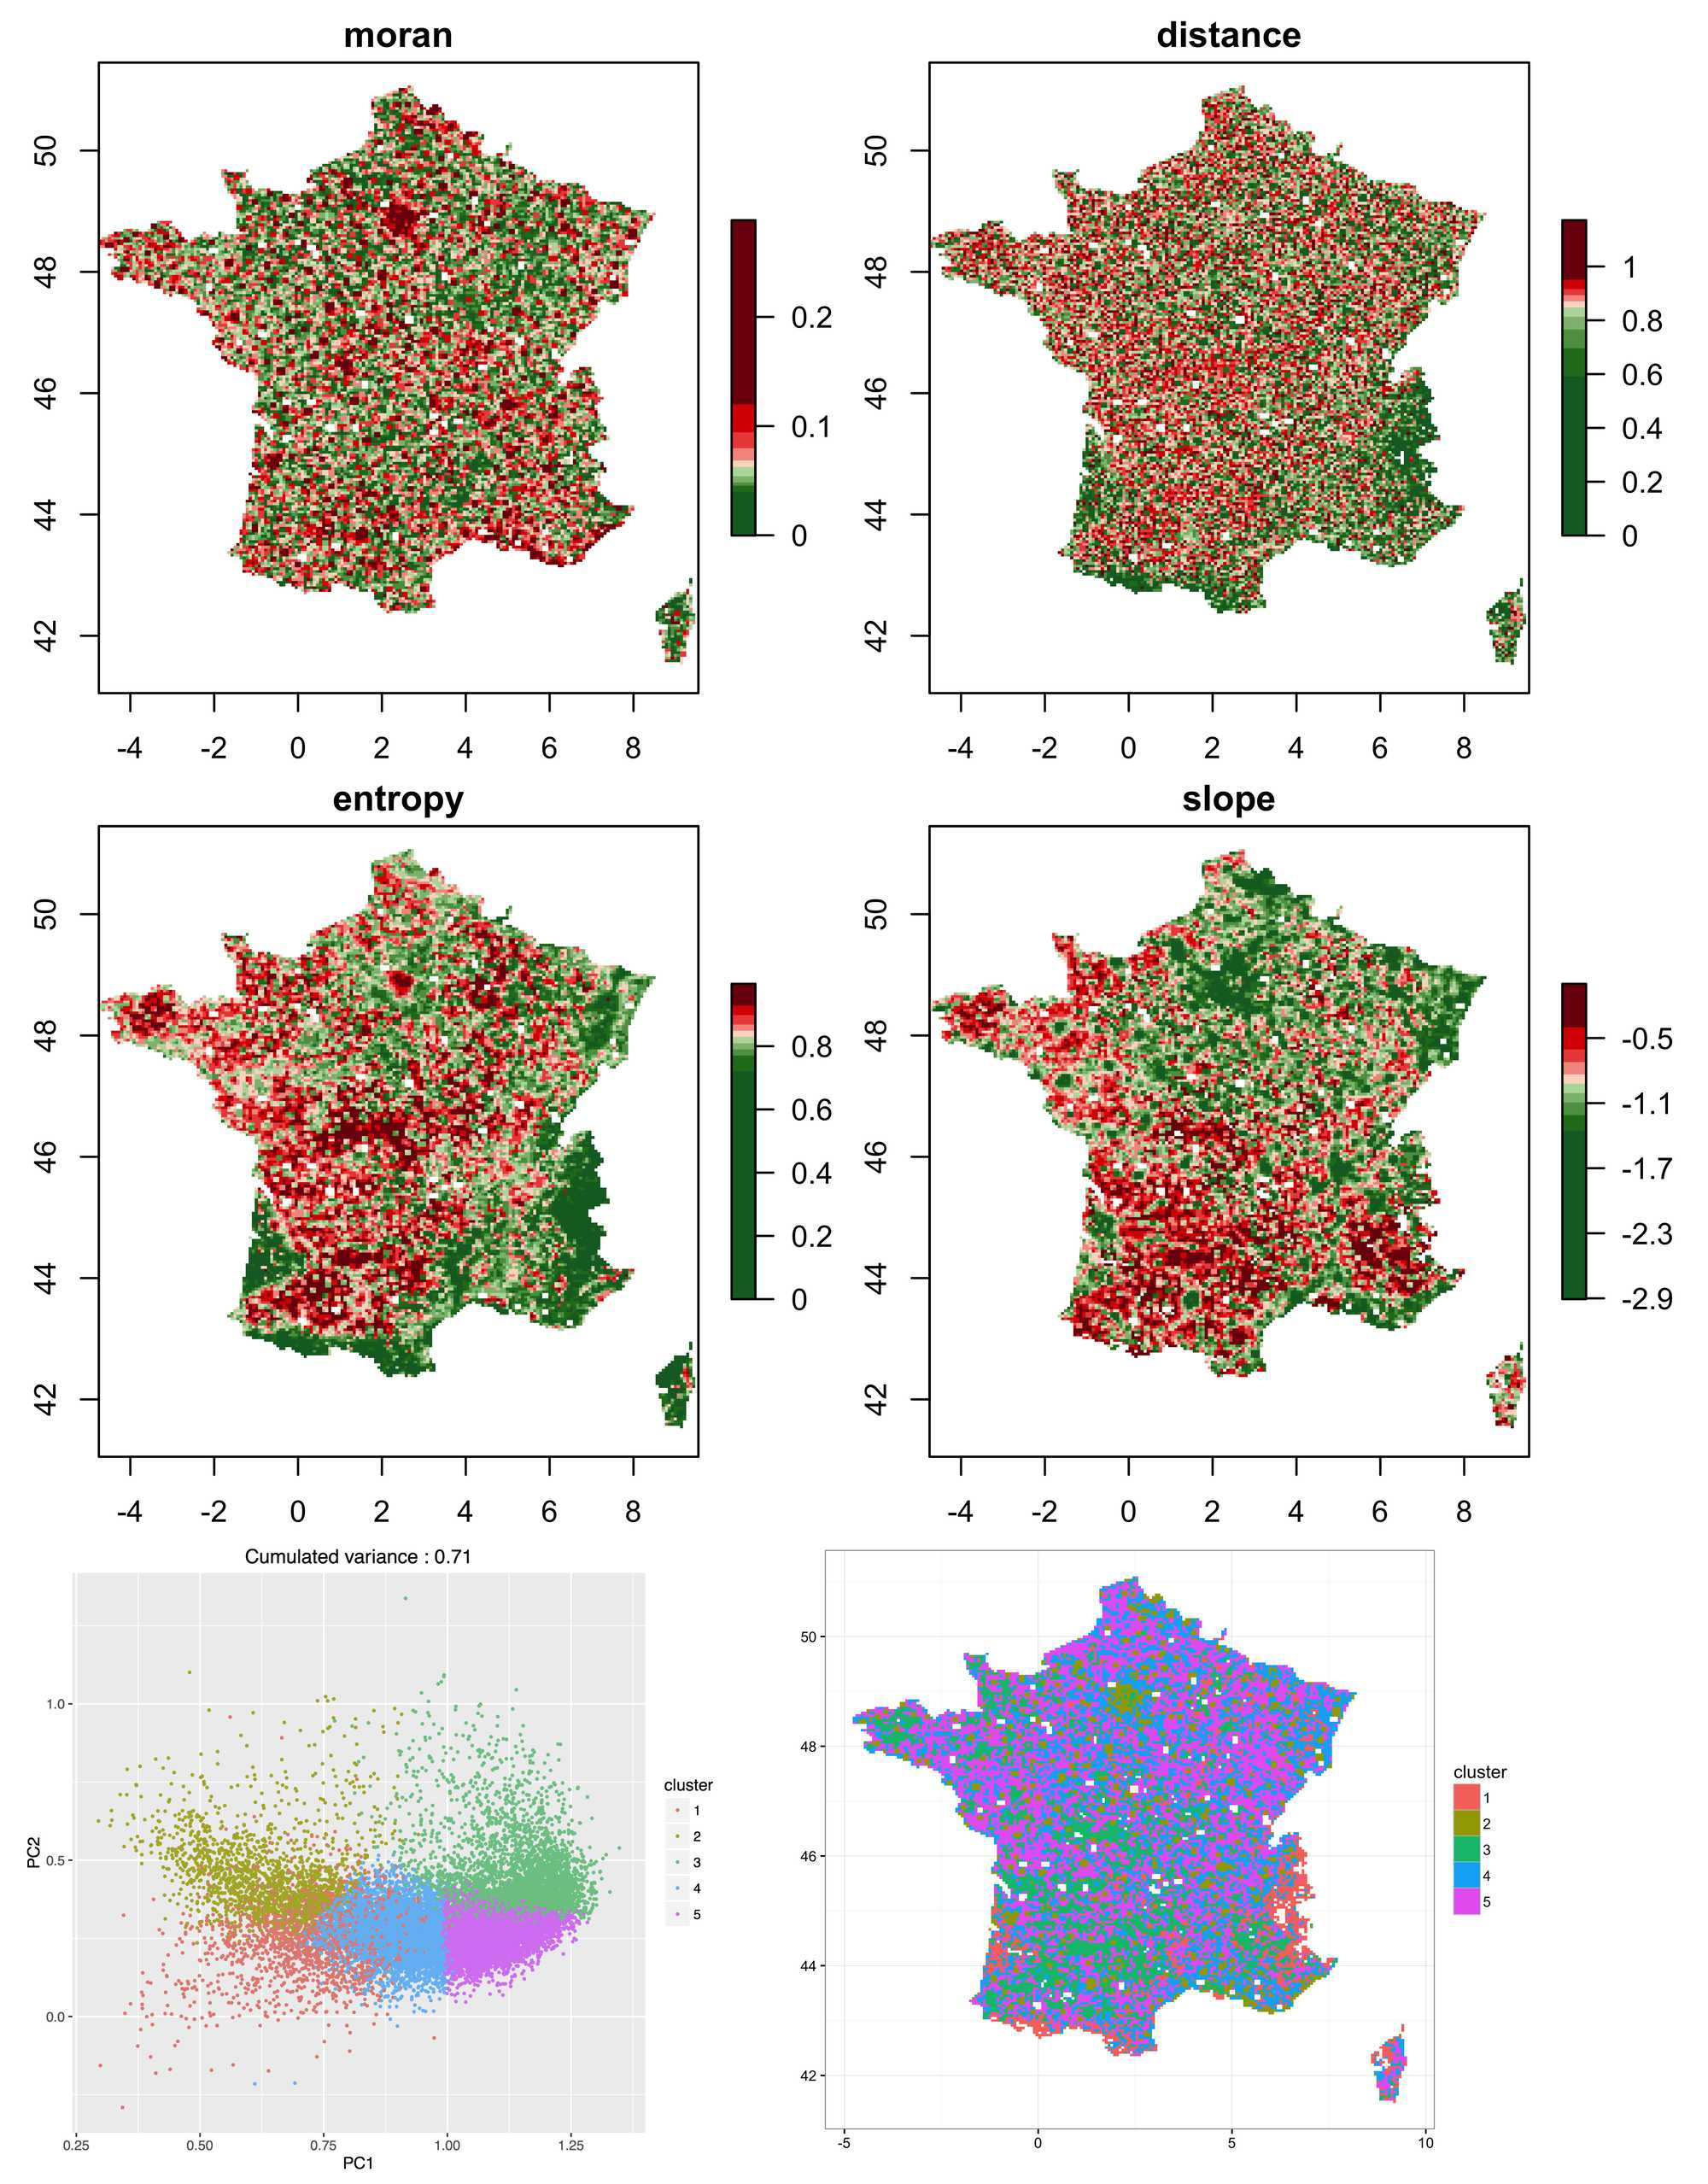
\includegraphics[width=0.9\linewidth]{Figures/Final/4-1-1-fig-staticcorrelations-empirical}
%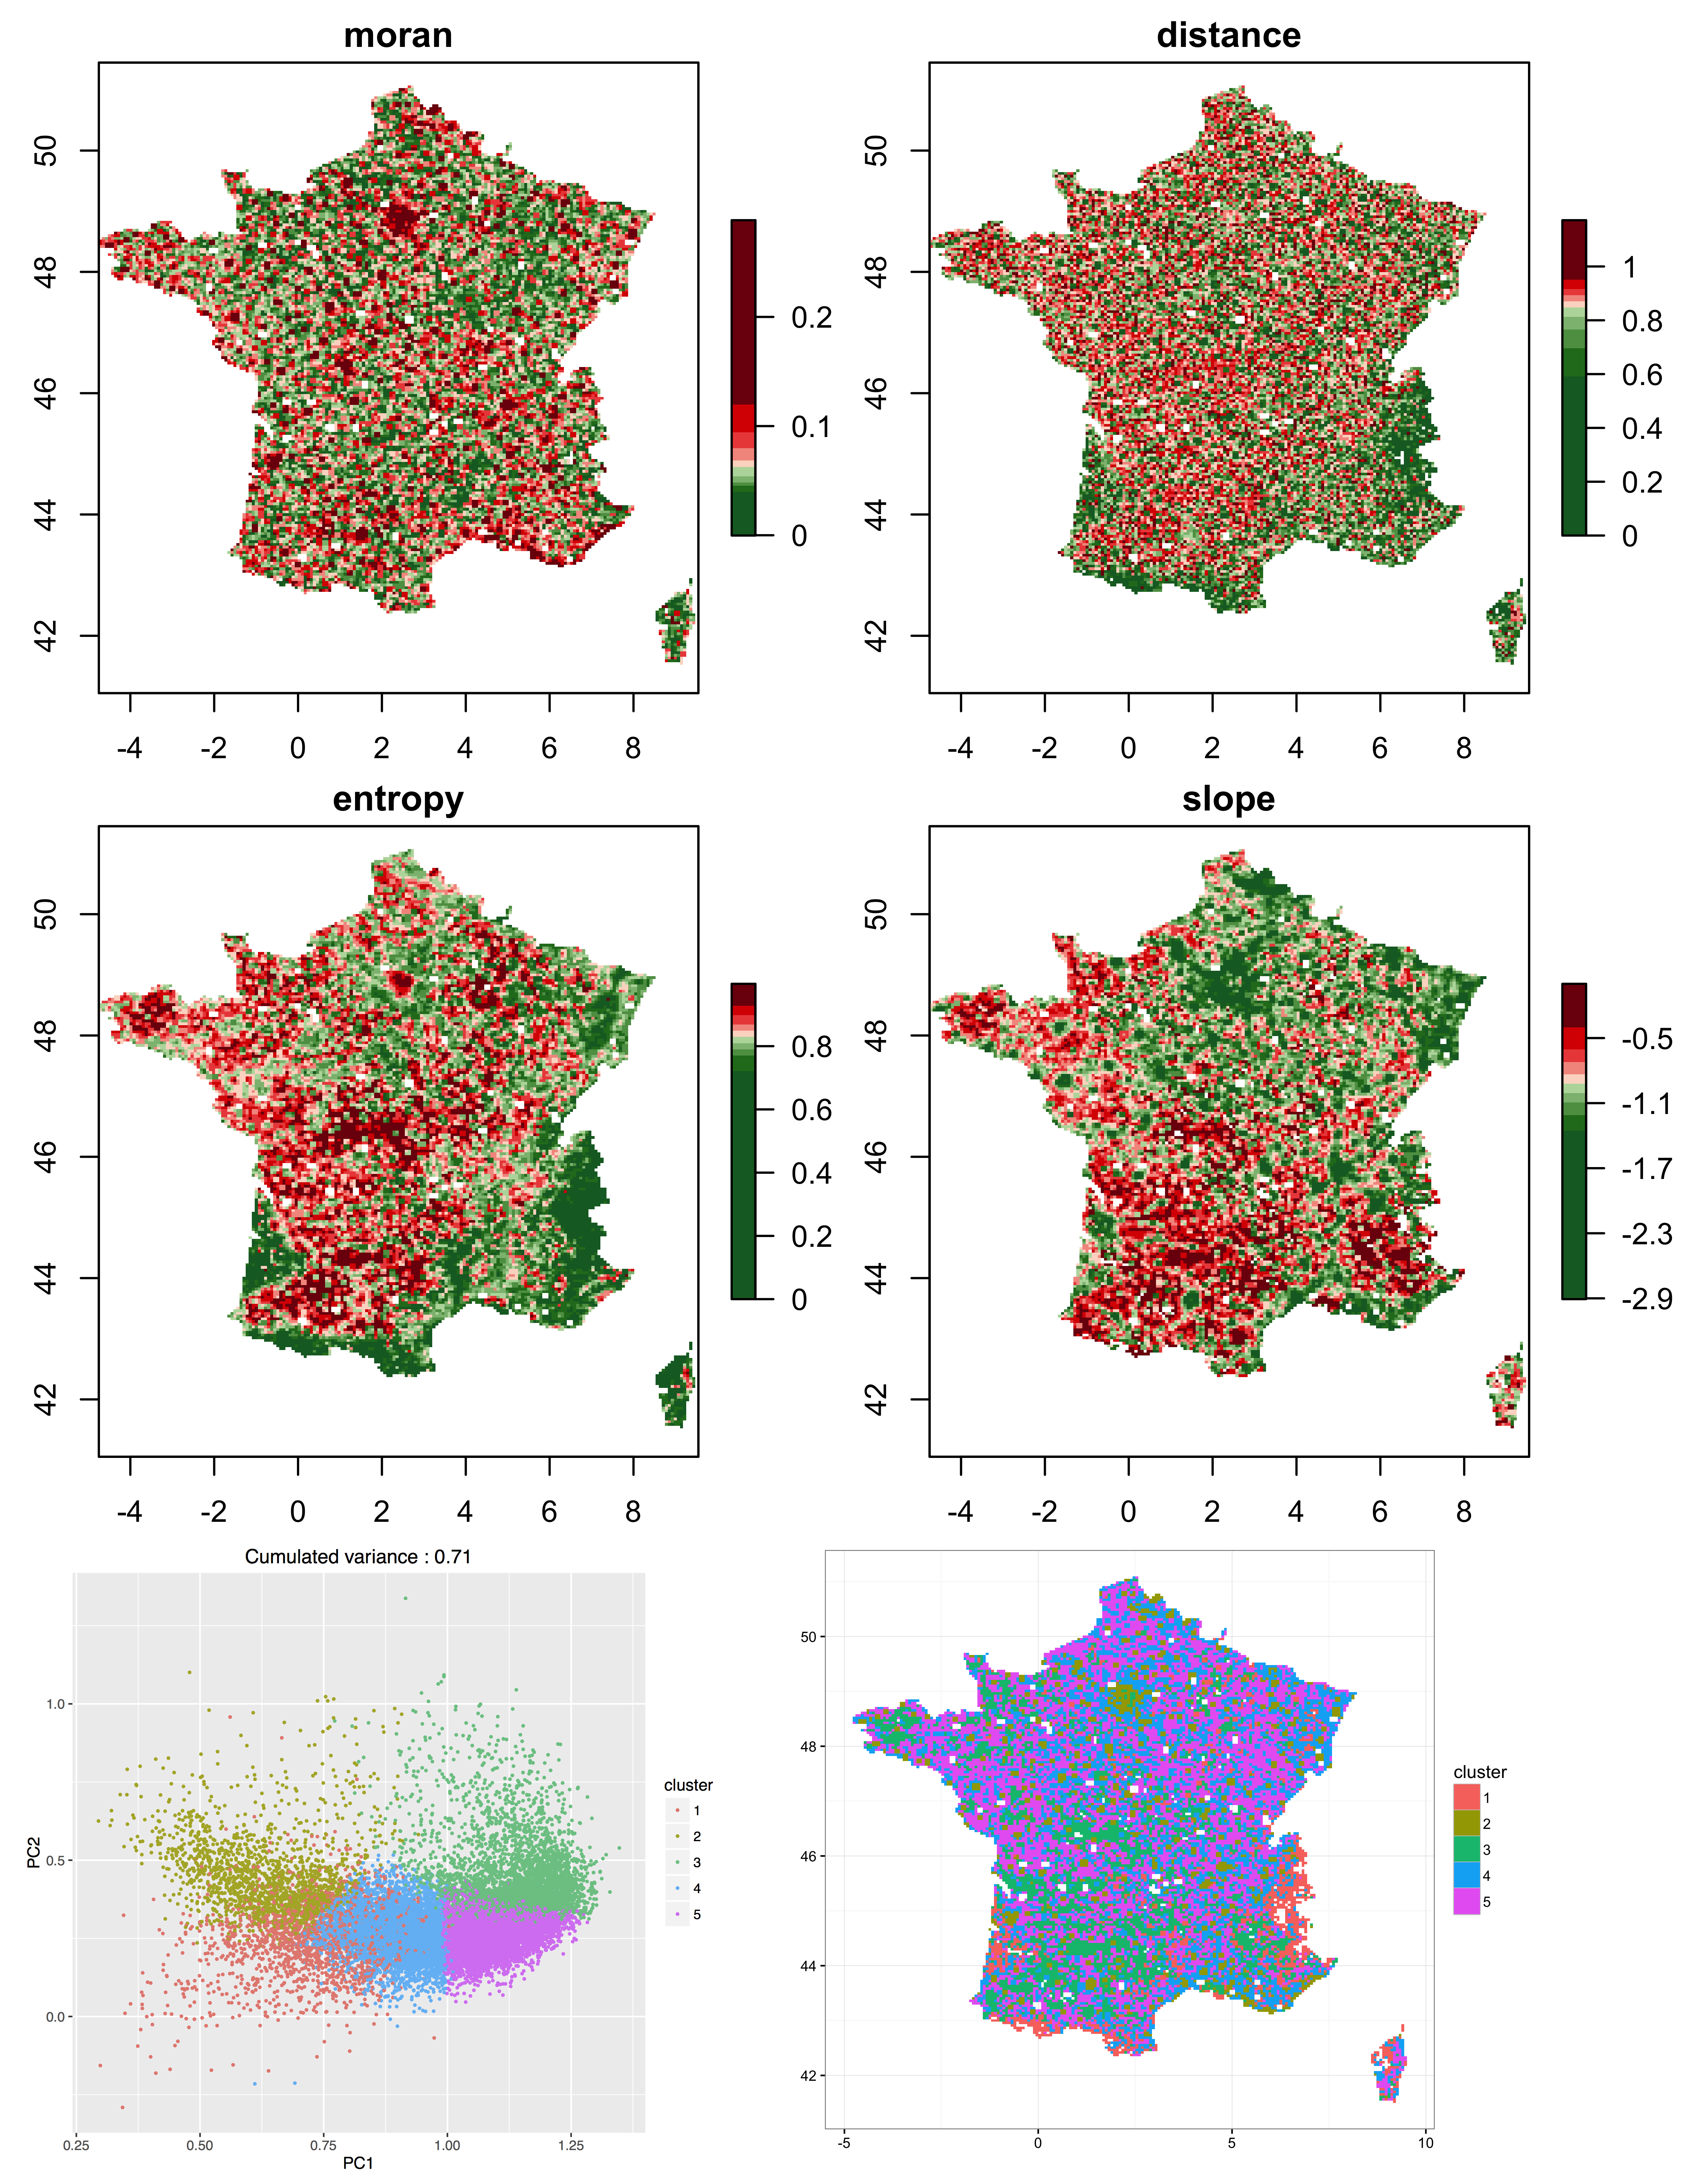
\includegraphics[width=0.9\linewidth]{Figures/Density/Fig1}
%\includegraphics[width=\textwidth]{figures/indics_morpho_discrquantiles}\\
%\includegraphics[width=0.49\textwidth]{figures/cluster_pca_k5_morpho}
%\includegraphics[width=0.49\textwidth]{figures/cluster_map_k5_morpho}
\caption[Empirical values of morphological indicators][Distribution spatiale des morphologies]{\textbf{Empirical values of morphological indicators.} \textit{(Top four maps)} Spatial distribution of the morphological indicators for France. Scale color discretization is done using quantiles to ease map readability. \textit{(Bottom Left)} Projection of morphological values on the two first components on a Principal Component analysis. Color gives cluster in an unsupervised classification (see text). \textit{(Bottom right)} Spatial distribution of clusters.\label{fig:staticcorrelations:empirical}}{\textbf{Valeurs empiriques des indicateurs morphologiques.} \textit{(Quatre cartes du haut)} Distribution spatiale des indicateurs morphologiques pour la France. La détermination de l'échelle de couleur est faite par quantiles pour faciliter la lecture des cartes. \textit{(Bas gauche)} Projection des valeurs morphologiques sur les deux premières composantes d'une analyse en composantes principales. La couleur donne le cluster dans une classification non supervisée (voir texte). \textit{(Bas droite)} Distribution spatiale des clusters. Se référer au texte pour les détails sur la procédure d'estimation spatiale des indicateurs et sur la procédure de classification.\label{fig:staticcorrelations:empirical}}
\end{figure}
%%%%%%%%%%%%%%%%%%%%%%%%

%\comment[FL]{a quelle distance se fait la fenetre ? par ailleurs le gros pb est que tu ne parles pas de ville ; ce n'est pas lisible $\rightarrow$ montrer moins de resultats filtres.}


\bpar{
We compute the morphological measures given above on real urban density data, using the population density grid of the European Union at 100m resolution provided openly by Eurostat~\cite{eurostat}. The choice of the resolution, the spatial range, and the shape of the window on which indicators are computed, is made according to the thematic specifications given before. We consider 50km wide square windows to be in accordance with the expected spatial range of one model instance. As it also does not make sense to have a too detailed resolution because of data quality, we take $N=100$ and aggregate the initial raster data at a 500m resolution to meet this size on real windows. To have a rather continuous distribution of indicators in space, we overlap windows by setting an offset of 10km between each, what also somehow rules out the question of window shape bias by the ``continuity'' of values. We tested the sensitivity to window size by computing samples with 30km and 100km window sizes and obtained rather similar spatial distributions. We show in Fig.~\ref{fig:staticcorrelations:empirical} maps giving values of indicators for France only to ease maps readability. The first striking feature is the diversity of morphological patterns across the full territory. The auto-correlation is naturally high in Metropolitan areas, with the Parisian surroundings clearly detached. When looking at other indicators, it is interesting to denote regional regimes: rural areas have much less hierarchy in the South than in the North, whereas the average distance is rather uniformly distributed except for mountain areas. Regions of very high entropy are observed in the Center and South-West. To have a better insight into morphological regimes, we use unsupervised classification with a simple k-means algorithm, for which the number of clusters $k=5$ witnesses a transition in inter-cluster variance. The split between classes is plotted in Fig.~\ref{fig:empirical}, bottom-left panel, where we show measures projected on the two first components of a Principal Component Analysis (explaining 71\% of variance). The map of morphological classes confirms a North-South opposition in a background rural regime (clear green against blue), the existence of mountainous (red) and metropolitan (dark green) regimes. Such a variety of settlements forms will be the target for the model. We did similar analysis for China using the gridded population data from~\cite{fu1km}: maps are available in~\ref{app:sec:staticcorrelations}.
}{
Nous calculons les mesures morphologiques données ci-dessus sur des données réelles de densité, en utilisant la grille de population de l'Union Européenne à la résolution de 100m fournie de manière ouverte par Eurostat~\cite{eurostat}. Cette base a certains défauts de précision qui ont été reconnus~\cite{bretagnolle2016ville} mais nous agrégerons les données à un niveau suffisant pour les éviter. Le choix de la résolution, de la portée spatiale, et de la forme de la fenêtre sur laquelle les indicateurs sont calculés, sont faits suivant les spécifications thématiques précédentes. Nous considérons des fenêtres carrées de largeur 50km, ce qui permet de plus d'être en accord avec l'ontologie du modèle de morphogenèse que l'on développera en~\ref{sec:densitygeneration}. Comme cela ne fait pas sens d'avoir une résolution trop détaillée à cause de la qualité des données, nous agrégeons les données raster initiales à une résolution de 500m pour avoir des fenêtres de taille $N=100$. Pour obtenir une distribution des indicateurs relativement continue dans l'espace, nous superposons les fenêtres en posant un décalage de 10km entre chaque, ce qui d'une certaine façon résout le problème du biais de la forme de la fenêtre par la ``continuité'' des valeurs. Nous avons testé la sensibilité à la taille de la fenêtre en calculant des échantillons avec des tailles de 30km et 100km et avons obtenu des distributions spatiales assez similaires. L'implémentation des indicateurs doit être faite avec attention, puisque les complexités computationnelles peuvent atteindre $O(N^4)$ pour l'indice de Moran par exemple: nous utilisons la convolution par Transformée de Fourier Rapide, qui est une technique permettant de calculer l'indice de Moran avec une complexité en $O(\log^2 N \cdot N^2)$. Nous montrons en Fig.~\ref{fig:staticcorrelations:empirical} des cartes donnant les valeurs des indicateurs, pour la France seulement afin de permettre une lisibilité. Pour avoir une idée des valeurs typiques de chacun des indicateurs, on pourra se référer aux distributions empiriques données en Appendice~\ref{app:sec:staticcorrelations}. La première caractéristique frappante est la diversité des motifs morphologiques au travers de l'ensemble du territoire. L'auto-correlation est relativement haute dans les zones métropolitaines, avec les environs de Paris qui se détachent clairement. Lorsqu'on s'intéresse aux autres indicateurs, il est intéressant de constater des régimes régionaux: les zones rurales ont beaucoup moins de hiérarchie dans le Sud que dans le Nord, tandis que la distance moyenne est plutôt distribuée uniformément sauf dans les zones montagneuses. Des régions à très forte entropie sont observées dans le centre et le Sud-ouest. Pour avoir une meilleure compréhension des classes morphologiques existantes, nous utilisons une classification non-supervisée\footnote{qui consiste à partitioner l'espace des données selon leur structure endogène} avec un algorithme des k-means simple. Le nombre de clusters $k=5$ induit une transition dans la variance inter-cluster, ce qui signifie qu'une variation de structure opère à ce nombre, que nous choisissons alors comme nombre de clusters. La séparation entre les classes est montrée en~\ref{fig:staticcorrelations:empirical}, panneau bas gauche, où nous représentons les mesures projetées sur les deux premières composantes d'une Analyse en Composantes Principales (expliquant 71\% de la variance, ce qui est relativement conséquent). La carte des classes morphologiques confirme une opposition Nord-Sud dans le régime rural de fond (vert clair contre bleu), l'existence d'un régime de montagne (rouge) et d'un régime métropolitain (vert sombre). Une telle variété d'établissements sera l'un des objectifs du modèle en~\ref{sec:densitygeneration}. Un calcul similaire des indicateurs morphologiques a été effectué pour la Chine en utilisant la grille de population à 1km fournie par~\cite{fu1km}. Les cartes sont disponibles en Appendice~\ref{app:sec:staticcorrelations}.
}






%%%%%%%%%%%%%%%%%%
\subsection{Network Measures}{Mesures de Réseau}


\bpar{
We consider network aggregated indicators as a way to characterize transportation network properties on a given territory, the same way morphological indicators yielded information on urban structure. We propose to compute some simple indicators on same extents as for morphology, to be able to explore relations between these static measures. Static network analysis has been extensively documented in the literature, see for example \cite{louf2014typology} for a cross-sectional study of cities or \cite{2015arXiv151201268L} for exploration of new measures for the road network.
}{
Nous considérons d'autre part les mesures agrégées de réseau comme un moyen de caractériser les propriétés des réseaux de transport sur un territoire donné, de la même façon que les indicateurs morphologiques informent sur la structure urbaine. Nous proposons de calculer des indicateurs simples sur des étendues spatiales similaires à la morphologie, pour être en mesure d'explorer les relations entre ces mesures statiques. L'analyse statique de réseau a été intensément documentée dans la littérature, voir par example \cite{louf2014typology} pour une étude comparative des villes ou \cite{2015arXiv151201268L} pour l'exploration de nouvelles mesures pour le réseau de rues. \cite{2017arXiv170902939M} utilise des techniques issues de l'apprentissage profond pour établir une typologie des réseaux viaires urbains pour un grand nombre de villes dans le monde.
}


\subsubsection{Data preprocessing}{Pré-traitement des données}


\bpar{
We work here with the road network, which structure is finely conditioned to territorial configuration of population densities. Furthermore, data for present day road network is openly available through the OpenStreetMap project~\cite{openstreetmap}. Its quality was investigated for different countries such as England~\cite{haklay2010good} and France~\cite{girres2010quality}. It was found to be of a quality equivalent to official surveys for the primary road network. Concerning China, although \cite{zheng2014assessing} underlined a quick acceleration of OpenStreetMap road data completeness and accuracy, its use for computation of network indicators may be questioned at a very fine scale. \cite{zhang2015density} highlights four regimes of data quality, partitioning China into regions among which qualitative behavior of OSM data varies. We underline that the results will be more valid on the regions where the quality is the highest, i.e. with high density and high diversity.
}{
Nous travaillons ici avec le réseau de rues, dont la structure est finement conditionnée aux configurations territoriales des densités de population. De plus, les données du réseau de routes actuel est disponible ouvertement par l'intermédiaire du projet OpenStreetMap (OSM)~\cite{openstreetmap}. Sa qualité a été étudiée pour différents pays comme l'Angleterre~\cite{haklay2010good} et la France~\cite{girres2010quality}. Il a été établi pour ces pays une qualité équivalente aux données officielles pour le réseau de rues primaire, au sens à la fois de la couverture spatiale et de la précision locale. Dans le cas de la Chine, bien que \cite{zheng2014assessing} soulève une récente accélération de la complétude et de la précision des données OSM pour les routes, leur usage pour le calcul d'indicateurs de réseau peut être questionné à une échelle très fine. \cite{zhang2015density} souligne quatre régimes de qualité des données, fournissant une partition de la Chine en régions entre lesquelles le comportement qualitatif des données OSM varie. Nous devrons garder à l'esprit cette variabilité, et pour être assuré de la fiabilité des résultats, nous simplifierons le réseau à un niveau d'agrégation suffisant.
}




\bpar{
From the primary road segments, we compute the topological road network for all studied areas, at 100m granularity scale to be used consistently with the population grid. The OSM data is imported into \texttt{pgsql} using \texttt{osmosis}, is then aggregated at fixed granularity, and the resulting topological network is finally simplified with a split/merge algorithm. We have for Europe $\simeq 44\cdot 10^6$ links in initial OSM db, $\simeq 61\cdot 10^6$ in first simplified layer, $\simeq 21\cdot 10^6$ in final database. For a given dataset corresponding to a subset of the overall road network, it is necessary to simplify network structure by spatial aggregation as initial data presents very detailed features and thus a very large numbers of nodes ($\simeq 10^10$ for Europe dataset). It is possible to drastically reduce network size by spatial aggregation of nodes and link replacements. The detailed algorithm and implementation are detailed in Supplementary material~\ref{app:sec:staticcorrelations}.
}{
Pour les segments de rue primaires, nous calculons le réseau topologique pour l'ensemble des zones étudiées, à une granularité de 100m pour pouvoir être utilisé de manière cohérente avec les grilles de population et pour être robuste aux imperfections locales de codage ou données très locales manquantes. Les données OSM sont importées dans \texttt{pgsql} en utilisant \texttt{osmosis}~\cite{osmosis}. Le réseau est ensuite agrégé à la granularité fixe pour créer un graphe topologique, qui est finalement simplifié pour garder uniquement la structure topologique du réseau, les indicateurs normalisés étant relativement robustes à cette opération. Celle-ci est nécessaire pour un calcul simple des indicateurs et une cohérence thématique avec la couche de densité. On garde uniquement les noeuds ayant un degré strictement supérieur ou inférieur à deux, et les liaisons correspondantes, en prenant soin d'agréger la distance géographique réelle en construisant le lien topologique correspondant. Vu l'ordre de grandeur de taille des données (pour l'Europe, la base initiale a $\simeq 44.7\cdot 10^6$ liens, et la base finale simplifiée $\simeq 20.4\cdot 10^6$), un algorithme spécifique parallèle est mis en place, de structure \emph{split-merge}. Celui-ci est détaillé en Appendice~\ref{app:sec:staticcorrelations}.
}

%china 2048589 ; simpl 2022802
%europe 44706945 ; simpl 20443061

\subsubsection{Indicators}{Indicateurs}

\bpar{
These indicators are used to capture a rough picture of the structure. Refined work at smaller scales (intra-urban road network) and with more elaborated measures that allow to differentiate more precisely local form, was recently done by Lagesse in~\cite{2015arXiv151201268L}.
Network macroscopic structure is summarized by the following set of indicators, after the simplifications and reductions done in the previous step. Assuming network given by $N=(V,E)$, nodes spatial positions $\vec{x}(V)$ and edges \emph{effective distances} $d(E)$ taking into account impedances and real distances (to include basically network hierarchy), we have indicators:
}{
Nous introduisons des indicateurs pour avoir une idée large de la forme du réseau, utilisant un certain nombre d'indicateurs pour capturer le maximum de dimensions des propriétés des réseaux, plus ou moins liées à l'utilisation de ceux-ci. Ces indicateurs résumant la structure mesoscopique du réseau sont calculés sur les réseau topologiques obtenus par les étapes précédentes de simplification. Notant le réseau $N=(V,E)$, les noeuds ayant les positions spatiales $\vec{x}(v)$ et des populations $p(v)$ obtenus par agrégation de la population dans la partition de Dirichlet correspondante, les liens des \emph{distances effectives} $l(E)$ qui prennent en compte les impédances et les distance réelle (pour inclure la hiérarchie primaire du réseau), nous utilisons :
}

%"vcount"      "ecount" "gamma"   "meanDegree"   "mu"  "alpha"        "meanLinkLength"     "meanNodePop"        "meanClustCoef"      "components"        "meanBetweenness"    "alphaBetweenness"   "euclPerf"           "diameter"        "meanCloseness"      "alphaCloseness.x"   "meanTravelTime"     "alphaTravelTime.x"  "alphaAccessibility" "meanAccessibility"  "modularity"

\bpar{
\begin{itemize}
\item connectivity
\item degree distribution
\item centrality, taken as normalized mean \emph{betweenness-centrality}
\item average path length
\item network diameter
\item mean network speed
\end{itemize}
}{
\begin{itemize}
\item Caractéristiques basiques : nombre de noeuds $\left|V\right|$, nombre de lien $\left|E\right|$, densité $d$, degré moyen $\bar{\delta}$, nombre cyclotomique $\mu$, connectivité $\alpha$, longueur moyenne des liens $\bar{l}$, population moyenne $\bar{p}$, coefficient de clustering moyen $\bar{c}$, nombre de composantes $c_0$.
\item Mesures liées au plus courts chemins : diamètre $r$, performance euclidienne (définie par~\cite{banos2012towards}).
\item Mesures de centralité agrégées (le niveau de hiérarchie étant calculé par un ajustement OLS d'une loi rang taille) :
\begin{itemize}
\item \emph{Betweenness Centrality}, moyenne $\bar{bw}$ et hiérarchie $\alpha_{bw}$ : étant donné la distribution de la centralité sur l'ensemble des noeuds, on prend la pente d'un ajustement rang-taille ainsi que la moyenne de la distribution.
\item \emph{Closeness Centrality}, moyenne $\bar{cl}$ et hiérarchie $\alpha_{cl}$
\item Temps de trajet moyen vers les autres noeuds, moyenne $\bar{t}$ et hiérarchie $\alpha_{t}$
\item Accessibilité, qui correspond au temps de trajet pondéré par les populations, moyenne $\bar{a}$ et hiérarchie $\alpha_{a}$
\end{itemize}
\item Modularité
\end{itemize}
}

L'accessibilité est bien considérée comme un indicateur de réseau, puisque son calcul implique d'attribuer des poids aux noeuds par un population correspondante, et revient ensuite à un temps de trajet moyen pondéré. Cet indicateur est intéressant car à l'interface entre forme urbaine et forme du réseau, puisque la distribution de population sur les noeuds est prise en compte. On verra que celle-ci est fortement corrélée au même non-pondéré ($\rho = 0.86$ pour l'ensemble de la Chine par exemple).



\subsubsection{Network Shape and Resilience}{Forme de Réseau et Résilience}

L'idée fondamentale motivant le calcul d'indicateurs de réseau est d'obtenir une réduction de dimension drastique, s'il est possible d'associer certains ``types'' de réseau à des valeurs typiques d'indicateurs. On est très loin d'une connaissance fine de typologies qui associeraient propriétés topologiques, dynamiques et processus de génération du réseau, le tout dans des typologies. De même que de pouvoir relier systématiquement ces propriétés à des caractéristiques dérivées, comme la résilience qui est une propriété aux définitions diverses pour laquelle~\cite{Gao:2016ty} introduit une approche par la sensibilité des processus dynamiques. Afin d'illustrer d'une part la difficulté de caractériser les réseaux et d'autre part les potentialités offertes par notre base de données, nous développons en Appendice~\ref{app:sec:staticcorrelations} une courte analyse des propriétés de résilience au sens de~\cite{ash2007optimizing} pour des réseaux typiques.



\subsubsection{Results}{Résultats}


\bpar{}{
Les indicateurs de réseau ont été calculés sur les mêmes zones que les indicateurs de forme urbaine, pour pouvoir les mettre en correspondance directe et calculer les correlations par la suite. Nous montrons en Figure~\ref{fig:staticcorrs:network} un échantillon pour la France. Le comportement spatial des indicateurs est très instructif, et révèle comme pour la forme urbaine des régimes locaux (urbain, rural, métropolitain), mais aussi des régimes régionaux très marqués. Ceux-ci peuvent être dus au différentes pratiques agricoles selon les régions dans le cas du rural par exemple, impliquant une partition différente des parcelles ainsi qu'une organisation particulière de leur desserte. En taille du réseau, la Bretagne se détache nettement et rejoint les régions urbaines, témoignant d'un foncier très fragmenté. Cela est partiellement corrélé à une faible hiérarchie dans l'accessibilité. Le Sud et l'Est du Bassin Parisien étendu se distinguent par une forte Betweenness moyenne, en accord avec une forte hiérarchisation. Pour la Chine, pour laquelle une selection d'indicateurs est également donnée en~\ref{app:sec:staticcorrelations}, on observe des variation locales et régionales encore plus marquées, ainsi que par exemple les mega-régions urbaines qui se détachent, correspondant à un régime bien particulier.
}




%%%%%%%%%%%%%%%%%%%%%%%%
\begin{figure}
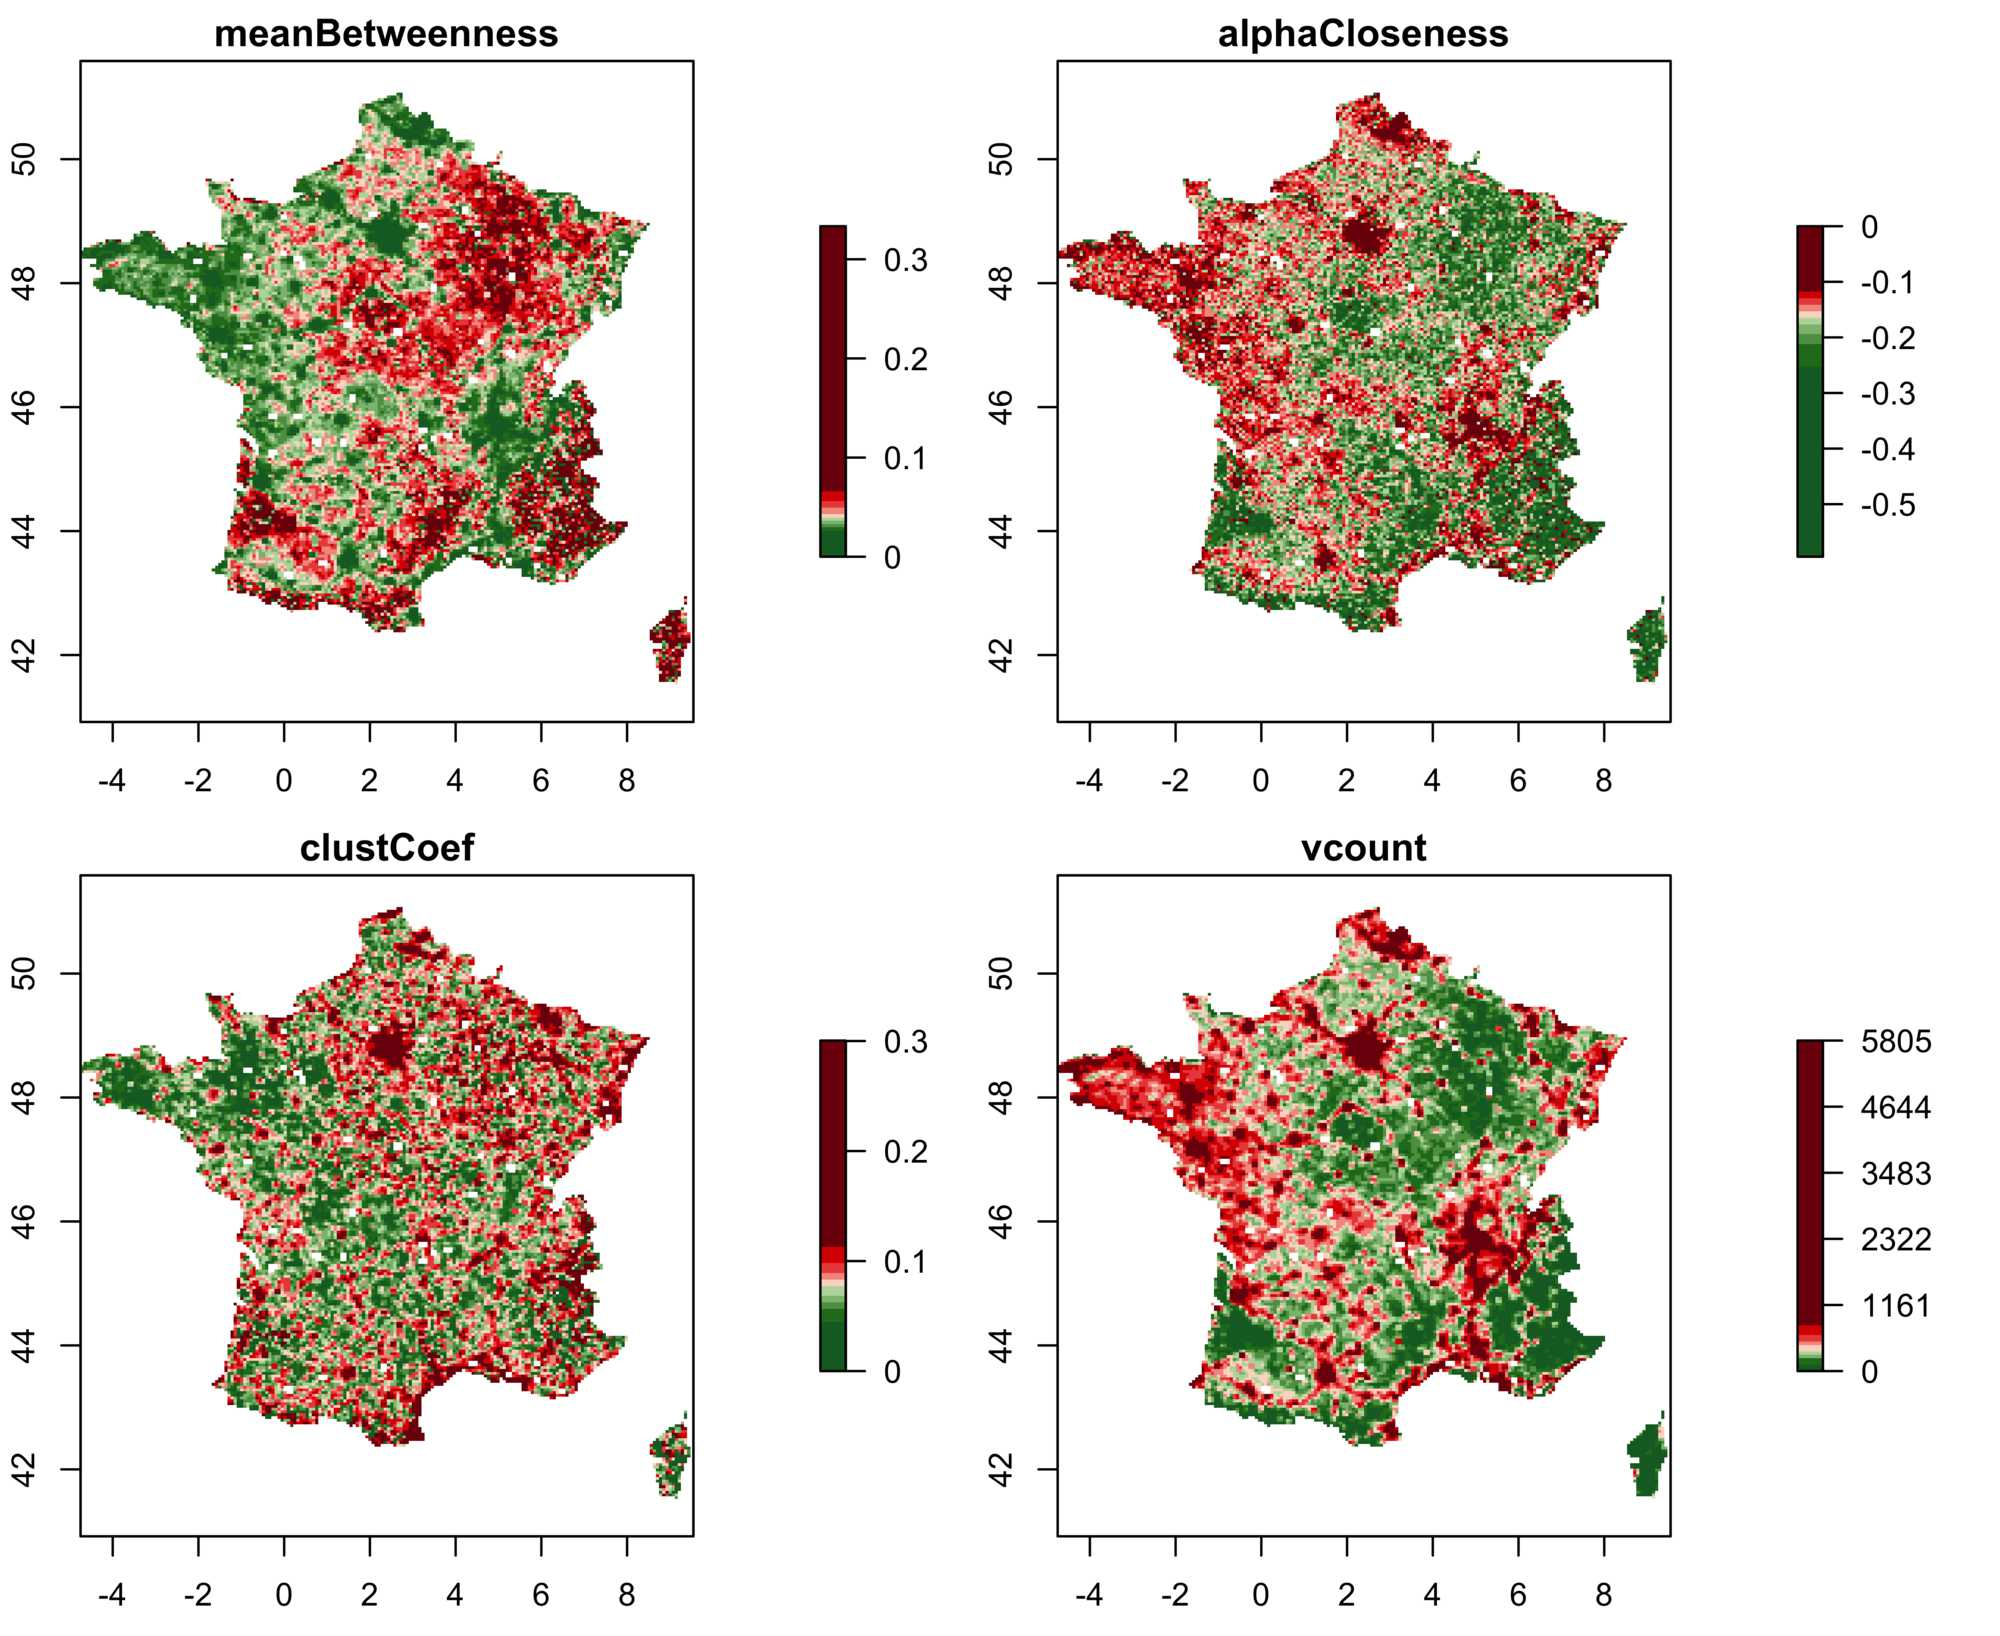
\includegraphics[width=\linewidth]{Figures/Final/4-1-2-fig-staticcorrs-network}
%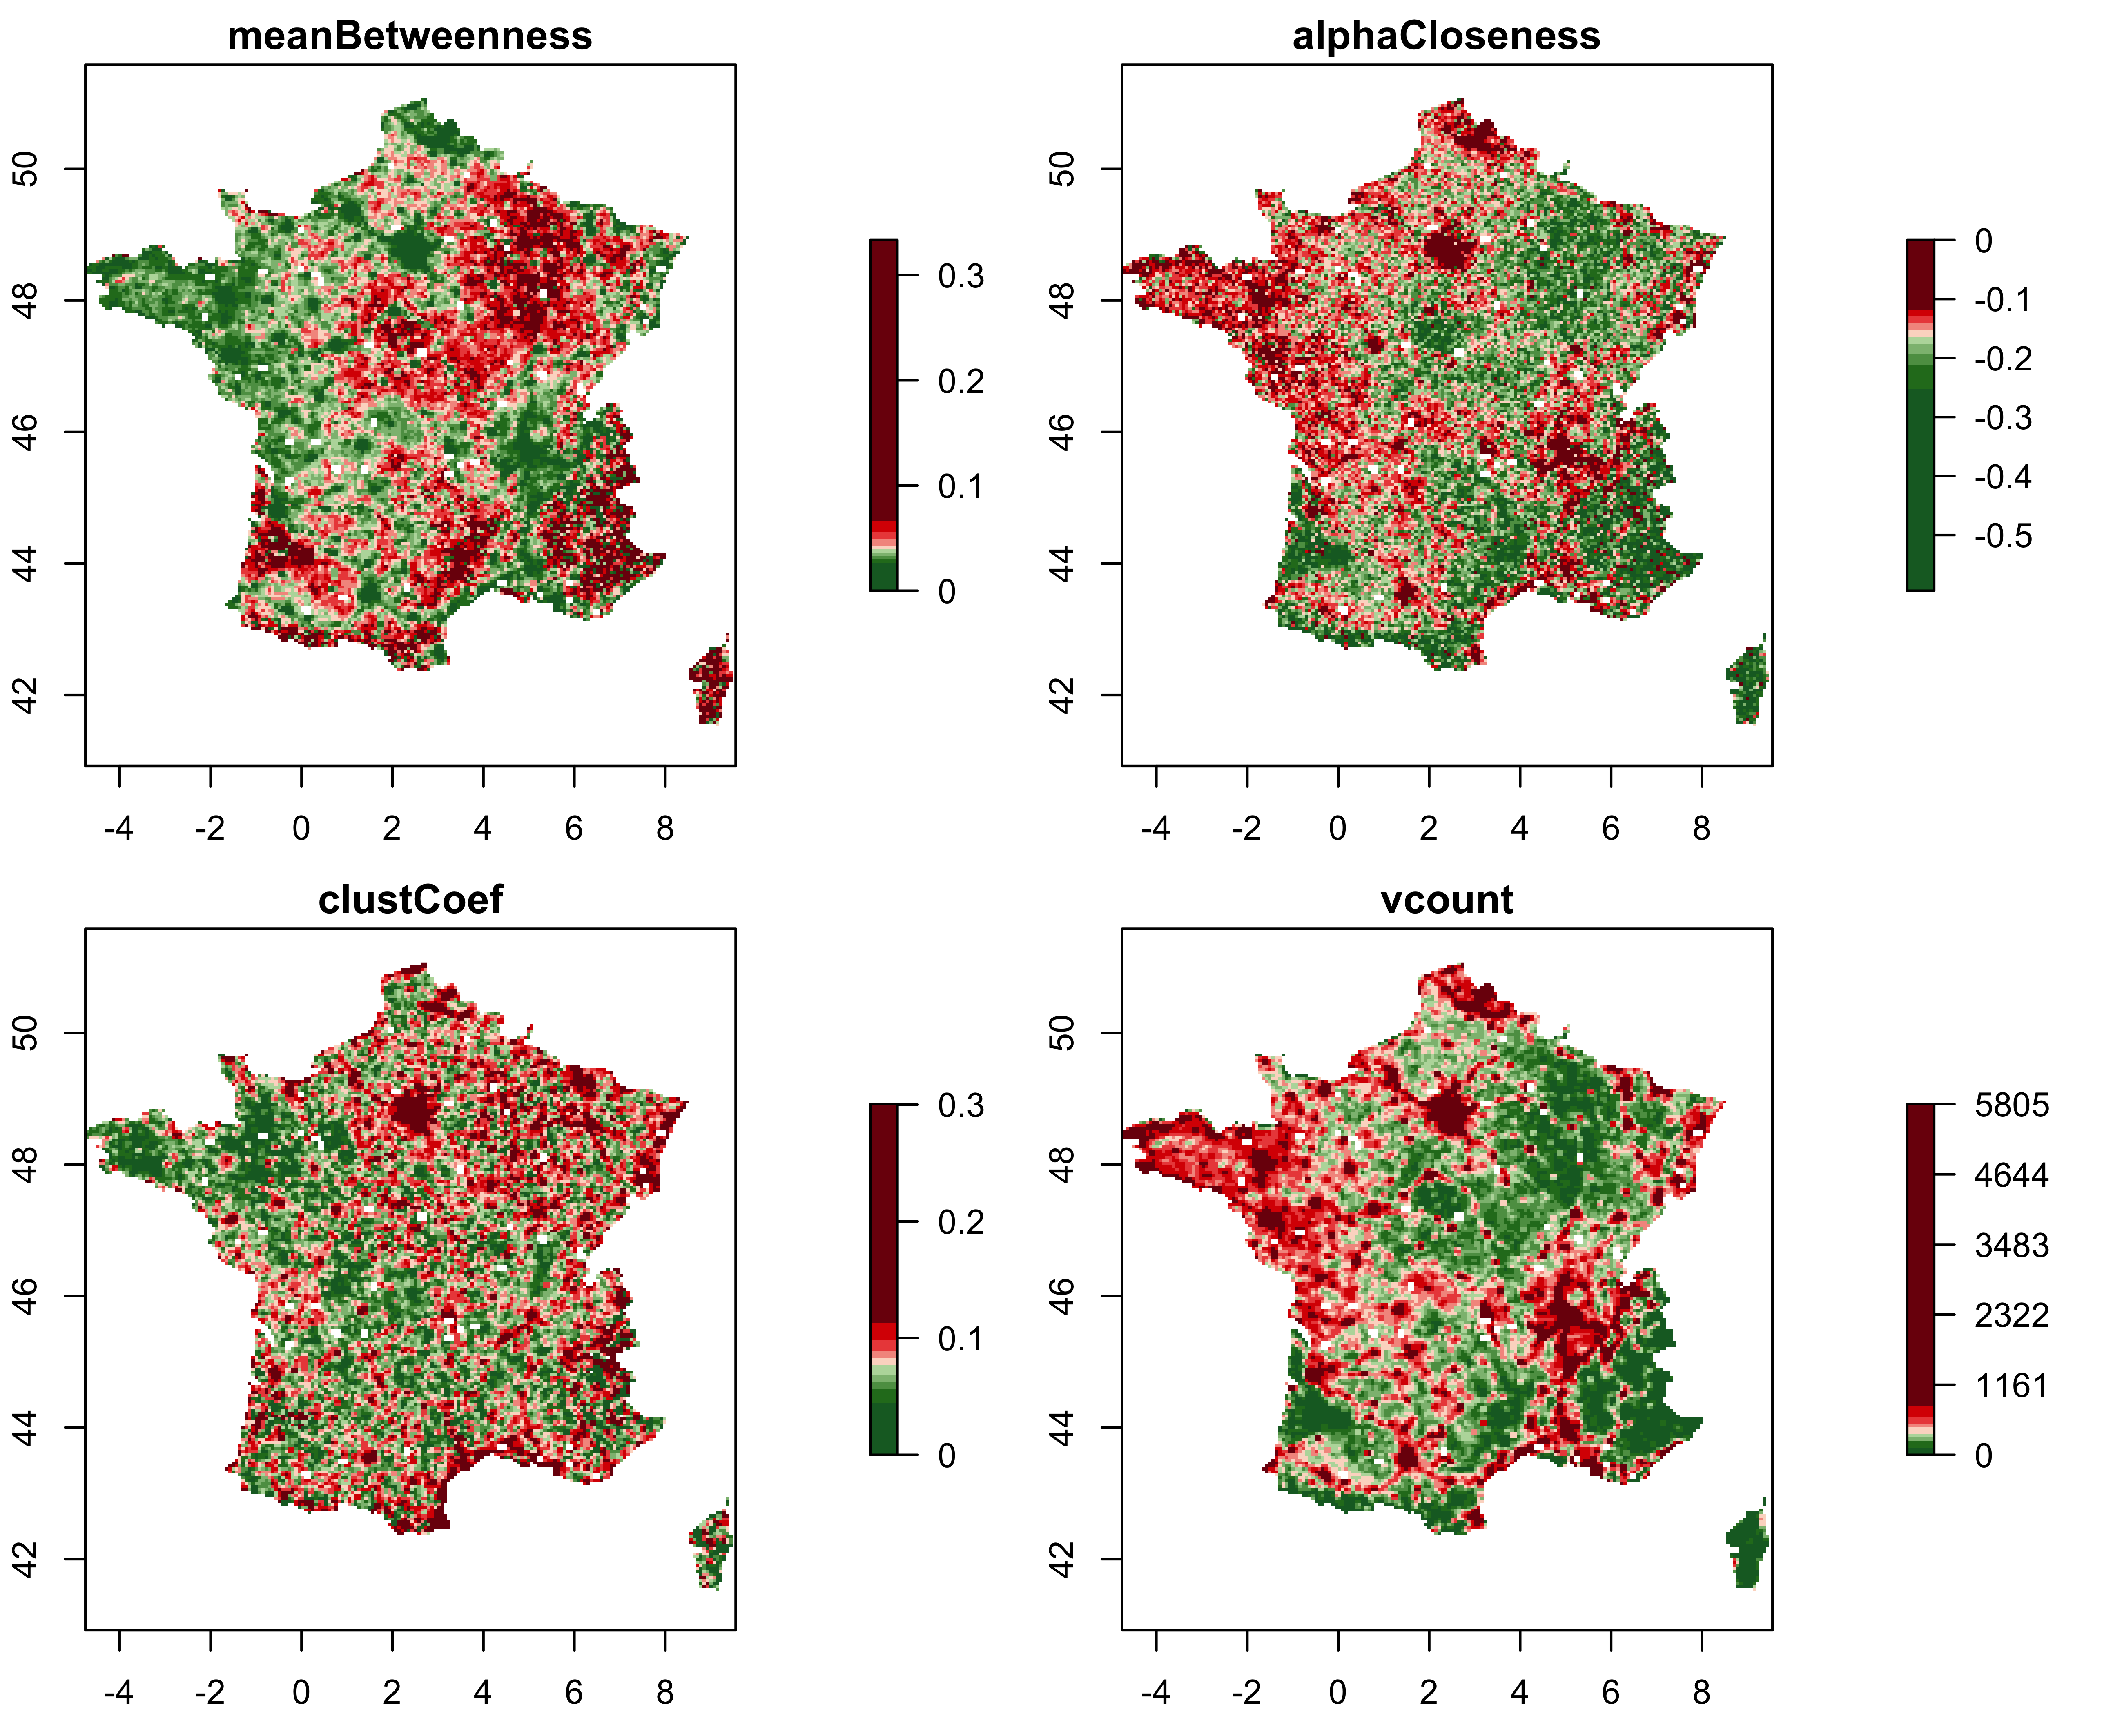
\includegraphics[width=\linewidth]{Figures/StaticCorrelations/FR_indics_network_selected_2_discrquantiles}
\caption[Empirical values of network indicators][Distribution spatiale des indicateur de réseau]{\textbf{Empirical values of network indicators.}\label{fig:staticcorrs:network}}{\textbf{Distribution spatiale des indicateur de réseau.} Nous donnons les indicateurs pour la France, en correspondance avec les indicateurs morphologiques décrits précédemment.\label{fig:staticcorrs:network}}
\end{figure}
%%%%%%%%%%%%%%%%%%%%%%%%





%%%%%%%%%%%%%%%%%%
\subsection{Effective static correlations}{Correlations Statiques Effectives et Non-stationnarité}


%%%%%%%%%%%%%%%%%%
%\subsubsection{Correlations}{Corrélations}
% short overview of overall correlations and effective dimensions
% not really needed



%%%%%%%%%%%%%%%%%%
\paragraph{Spatial Correlations}{Corrélations spatiales}


\bpar{
Pour les correlations : zones de correlation pas trop grandes, carrés de base indicateurs plus petits : Computation of urban form indicators~\cite{le2015forme} and network indicators on $l_0=10km$ side square. Computation of spatial correlation on square areas of width $\delta\cdot l_0$ (with typically $\delta = 4, \ldots , 16$) We clearly unveil the local spatial stationarity of processes.
}{
Les corrélations spatiales locales sont calculées sur des fenêtres regroupant un certain nombre d'observation, et donc de fenêtres sur lesquelles les indicateurs ont été calculés. Notons $l_0$ (qui vaut 10km dans les résultats précédents) la résolution des distributions des indicateurs. L'estimation des corrélations s'effectue alors sur des carrés de taille $\delta\cdot l_0$ (avec $\delta$ pouvant varier typiquement de 4 à 16). La valeur de $\delta$ influe directement sur le nombre d'observations, et donc la fiabilité de l'estimation. Nous montrons en Figure~\ref{fig:staticcorrs:mapscorrs} des exemples de corrélations estimées avec $\delta = 12$ dans le cas de la France. Avec 29 indicateurs, la matrice de corrélation est assez conséquente en taille, mais la dimension effective est réduite : une analyse en composante principale montre que $p=10$ capture 60\% de la variance, et la première composante capture déjà 16\%, ce qui est considérable dans un espace où la dimension avoisine les 800. On peut s'intéresser aux sous-blocs morphologique, de réseau, ou les corrélations croisées, qui exprime directement un lien entre les propriétés de la forme urbaine et celles du réseau. Par exemple, la relation entre Betweenness moyenne et hiérarchie morphologique que l'on visualise permet de comprendre la processus correspondant à la correspondance des hiérarchies : une population hiérarchisée peut induire un réseau hiérarchisé ou le sens inverse, mais elle peut également induire un réseau distribué ou celui-ci peut créer une hiérarchie de population - il faut bien comprendre en terme de correspondance et non de causalité, mais cette correspondance inform sur différents régimes urbains. Les métropoles semblent exhiber une corrélation positive dans ce cas, et des espaces ruraux négatifs. Cela suggère une très grande variété de régimes d'interaction. La variation spatiale de la première composante confirme celle-ci, ce qui révèle clairement la non-stationnarité spatiale des processus d'interaction entre formes, puisque les premiers et second moments varient dans l'espace. Nous donnons en Appendice~\ref{app:sec:staticcorrelations} d'autres exemples, pour l'ensemble de l'Europe et la Chine. Ces propriétés de non-stationnarité sont régulières pour l'ensemble de ces cas d'étude.
}



%%%%%%%%%%%%%%%%%%%%%%%%
\begin{figure}[h!]
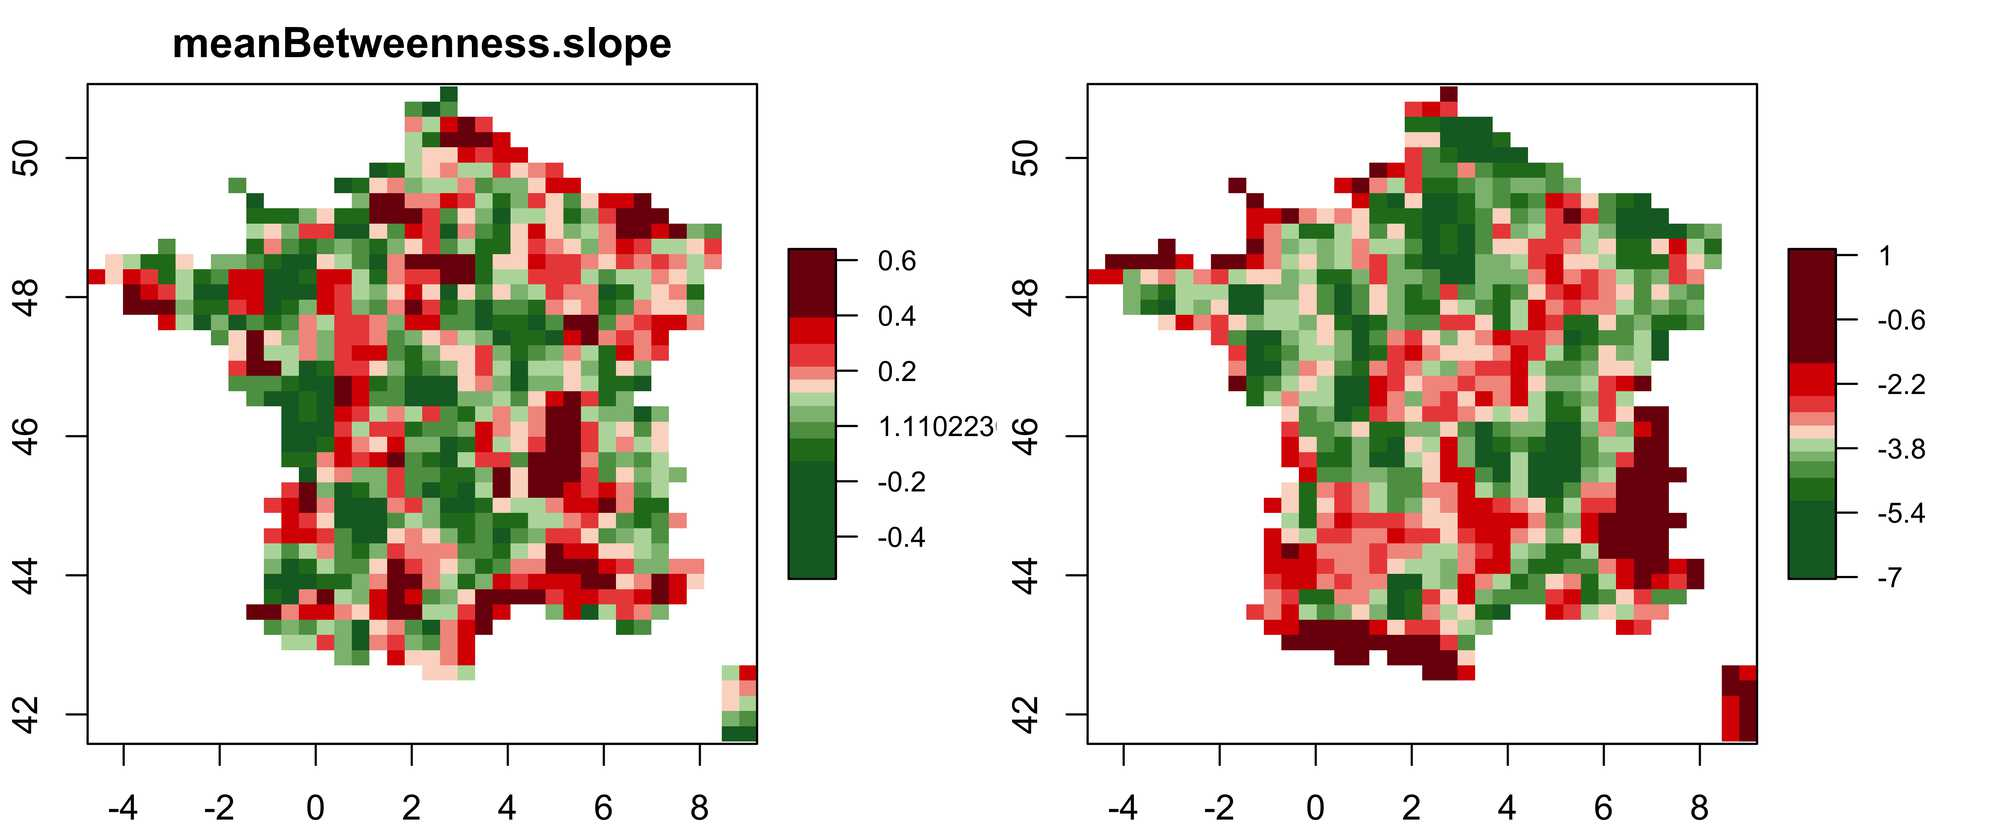
\includegraphics[width=\linewidth]{Figures/Final/4-1-3-fig-staticcorrs-mapscorrs}
%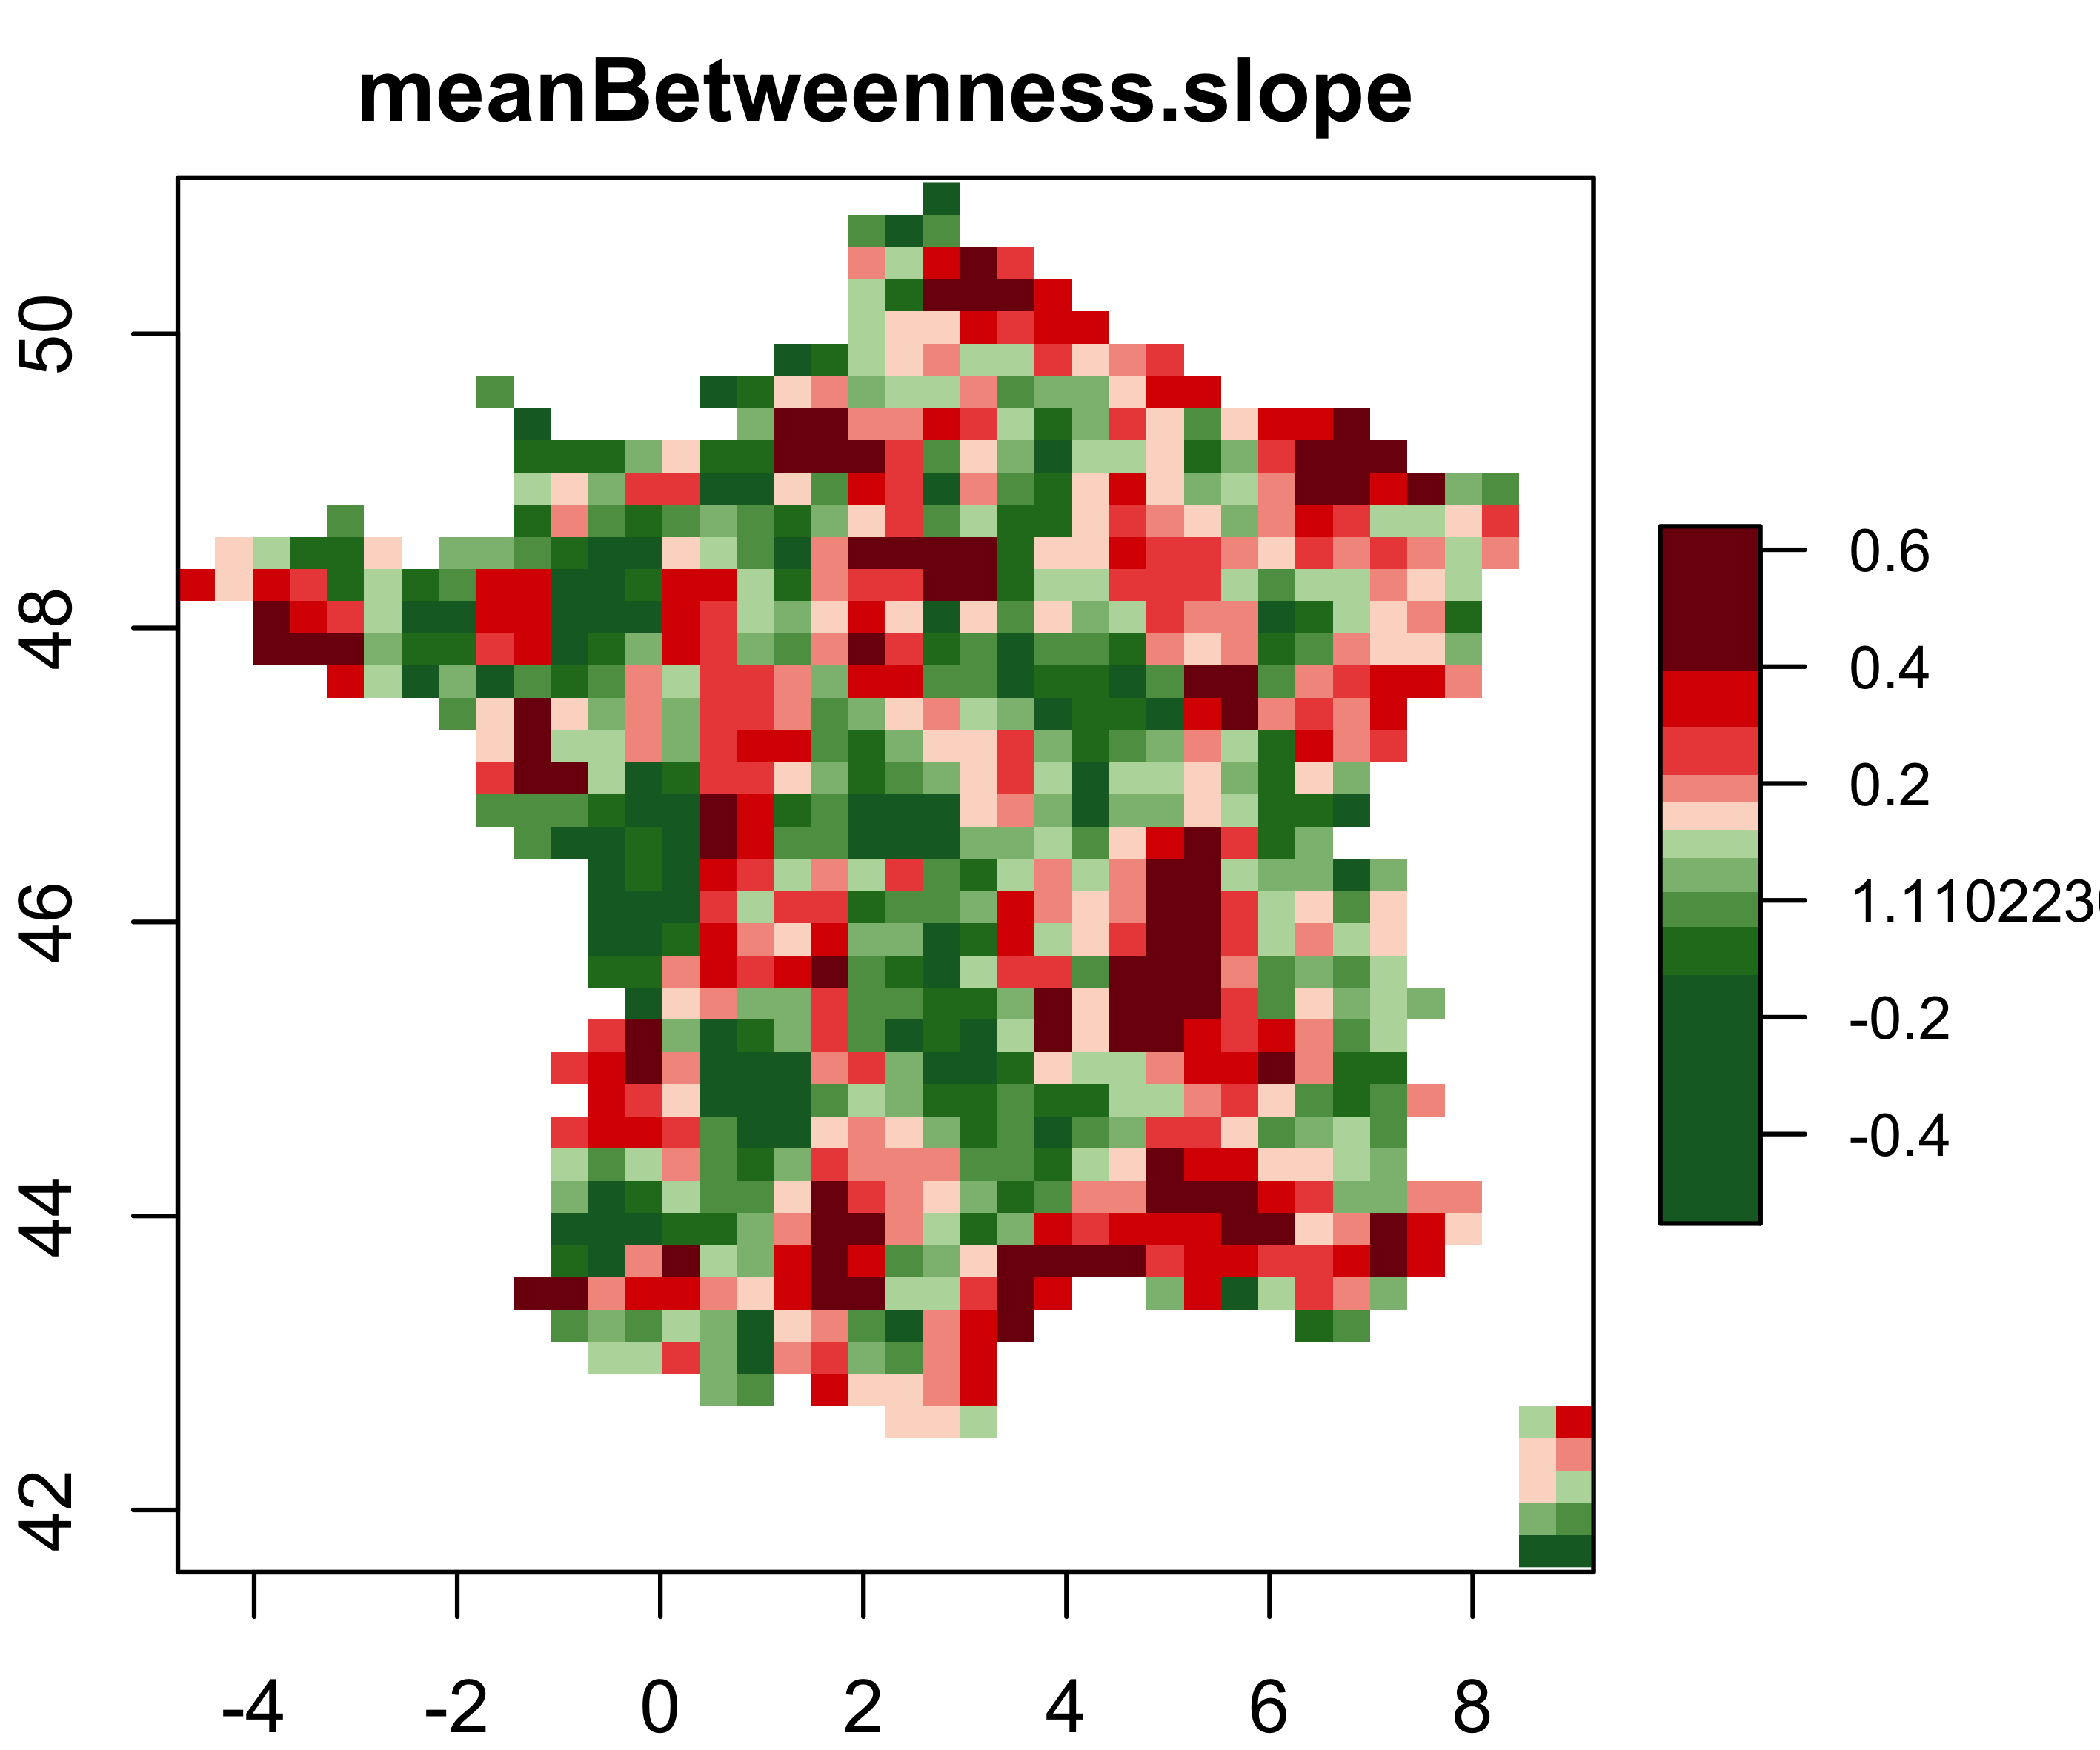
\includegraphics[width=0.48\linewidth]{Figures/StaticCorrelations/FR_corr_meanBetweenness_slope_rhoasize12}
%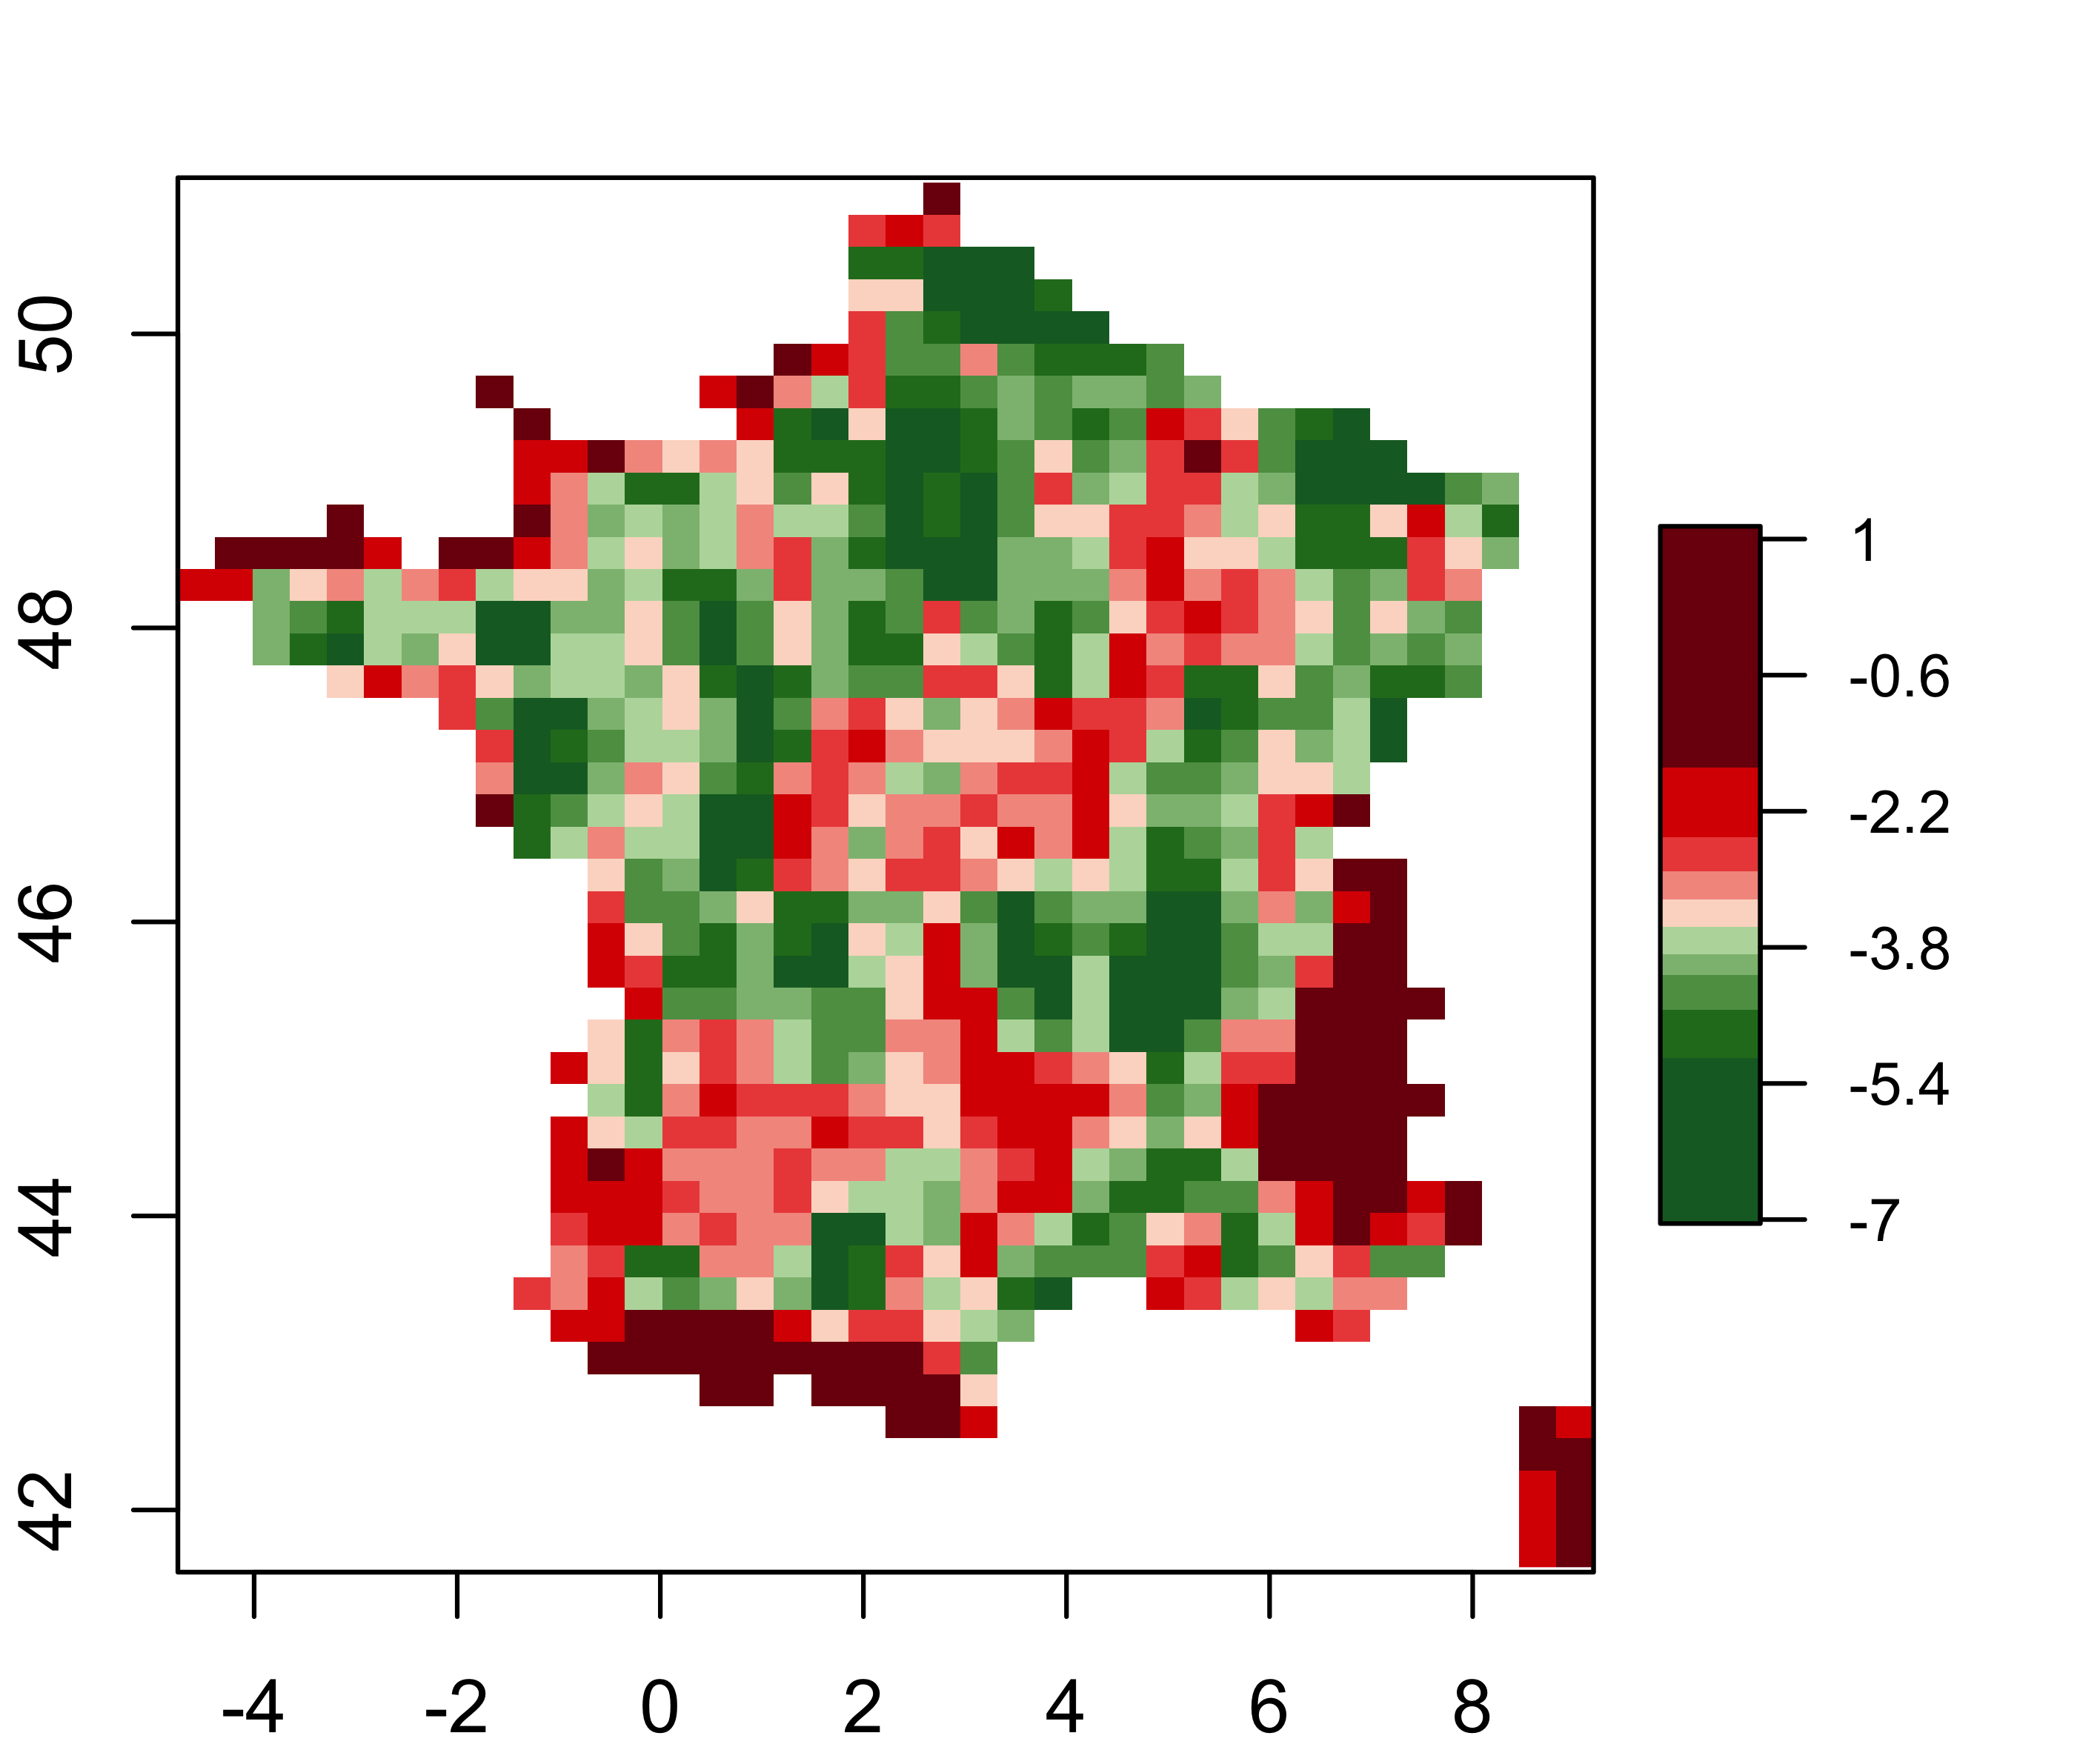
\includegraphics[width=0.48\linewidth]{Figures/StaticCorrelations/FR_corr_PCA_rhoasize12}
\caption[Spatial Correlations][Corrélations Spatiales]{Spatial Correlations\label{fig:staticcorrs:mapscorrs}}{\textbf{Exemples de corrélations Spatiales.} Pour la France, les cartes donnent $\rho\left[\bar{bw},\gamma\right]$ (gauche) et la première composante de la matrice réduite (droite).\label{fig:staticcorrs:mapscorrs}}
\end{figure}
%%%%%%%%%%%%%%%%%%%%%%%%



%%%%%%%%%%%%%%%%%%
\paragraph{Multi-scale Processes}{Nature multi-scalaire des processus}

\bpar{
$\rightarrow$ Significant variation of mean correlation with $\delta$ (Left) and of normalized confidence interval (Right) given by $\left|\rho_+ - \rho_-\right|\cdot \delta$, as bounds theoretically vary as $\sqrt{N} \sim \sqrt{\delta^2}$ : implies multi-scalarity
}{
On observe une variation significative des correlations fonction de $\delta$, qui se reflète dans la valeur moyenne de la matrice. D'abord, la distribution statistique des corrélations suit une loi similaire à une log-normale pour la morphologie seule, et plutôt normale pour le réseau et le croisement, ce qui voudrait dire que certaines zones ont des contraintes morphologiques assez fortes tandis que la forme du réseau est plutôt libre. On montre en Figure~\ref{fig:staticcorrs:corrsdistrib} ces distributions et les résultats des expériences de variation de $\delta$ pour l'Europe. On constate sur les nuages de points que les configurations où les corrélations croisées sont les plus fortes correspondent à celles où morphologique et réseau sont également fortes, confirmant l'imbrication des processus dans ce cas. L'augmentation de $\delta$ cause pour l'ensemble un décalage dans le positif, mais également un rétrécissement de la distribution, ces deux effets se traduisant par une décroissance des corrélations absolues moyennes, qui se stabilisent approximativement pour les grandes valeurs de $\delta$. Cette variation est révélateur d'un comportement multi-échelle : le changement de la taille de la fenêtre ne devrait pas influer l'estimateur si un seul processus était sous-jacent, elle devrait seulement changer la robustesse de l'estimation. Or la variation de la taille de l'intervalle de confiance normalisée, qui en théorie sous hypothèse de normalité devrait conduire $\delta\cdot \left|\rho_+ - \rho -\right|$ à être constant dans ce cas (puisque les bornes varient comme $\sqrt{N}\sim \sqrt{\delta^2}$), confirme bien cette première hypothèse. Ainsi, les processus sont à la fois non-stationnaires et multi-scalaires.
}


%%%%%%%%%%%%%%%%%%%%%%%%
\begin{figure}
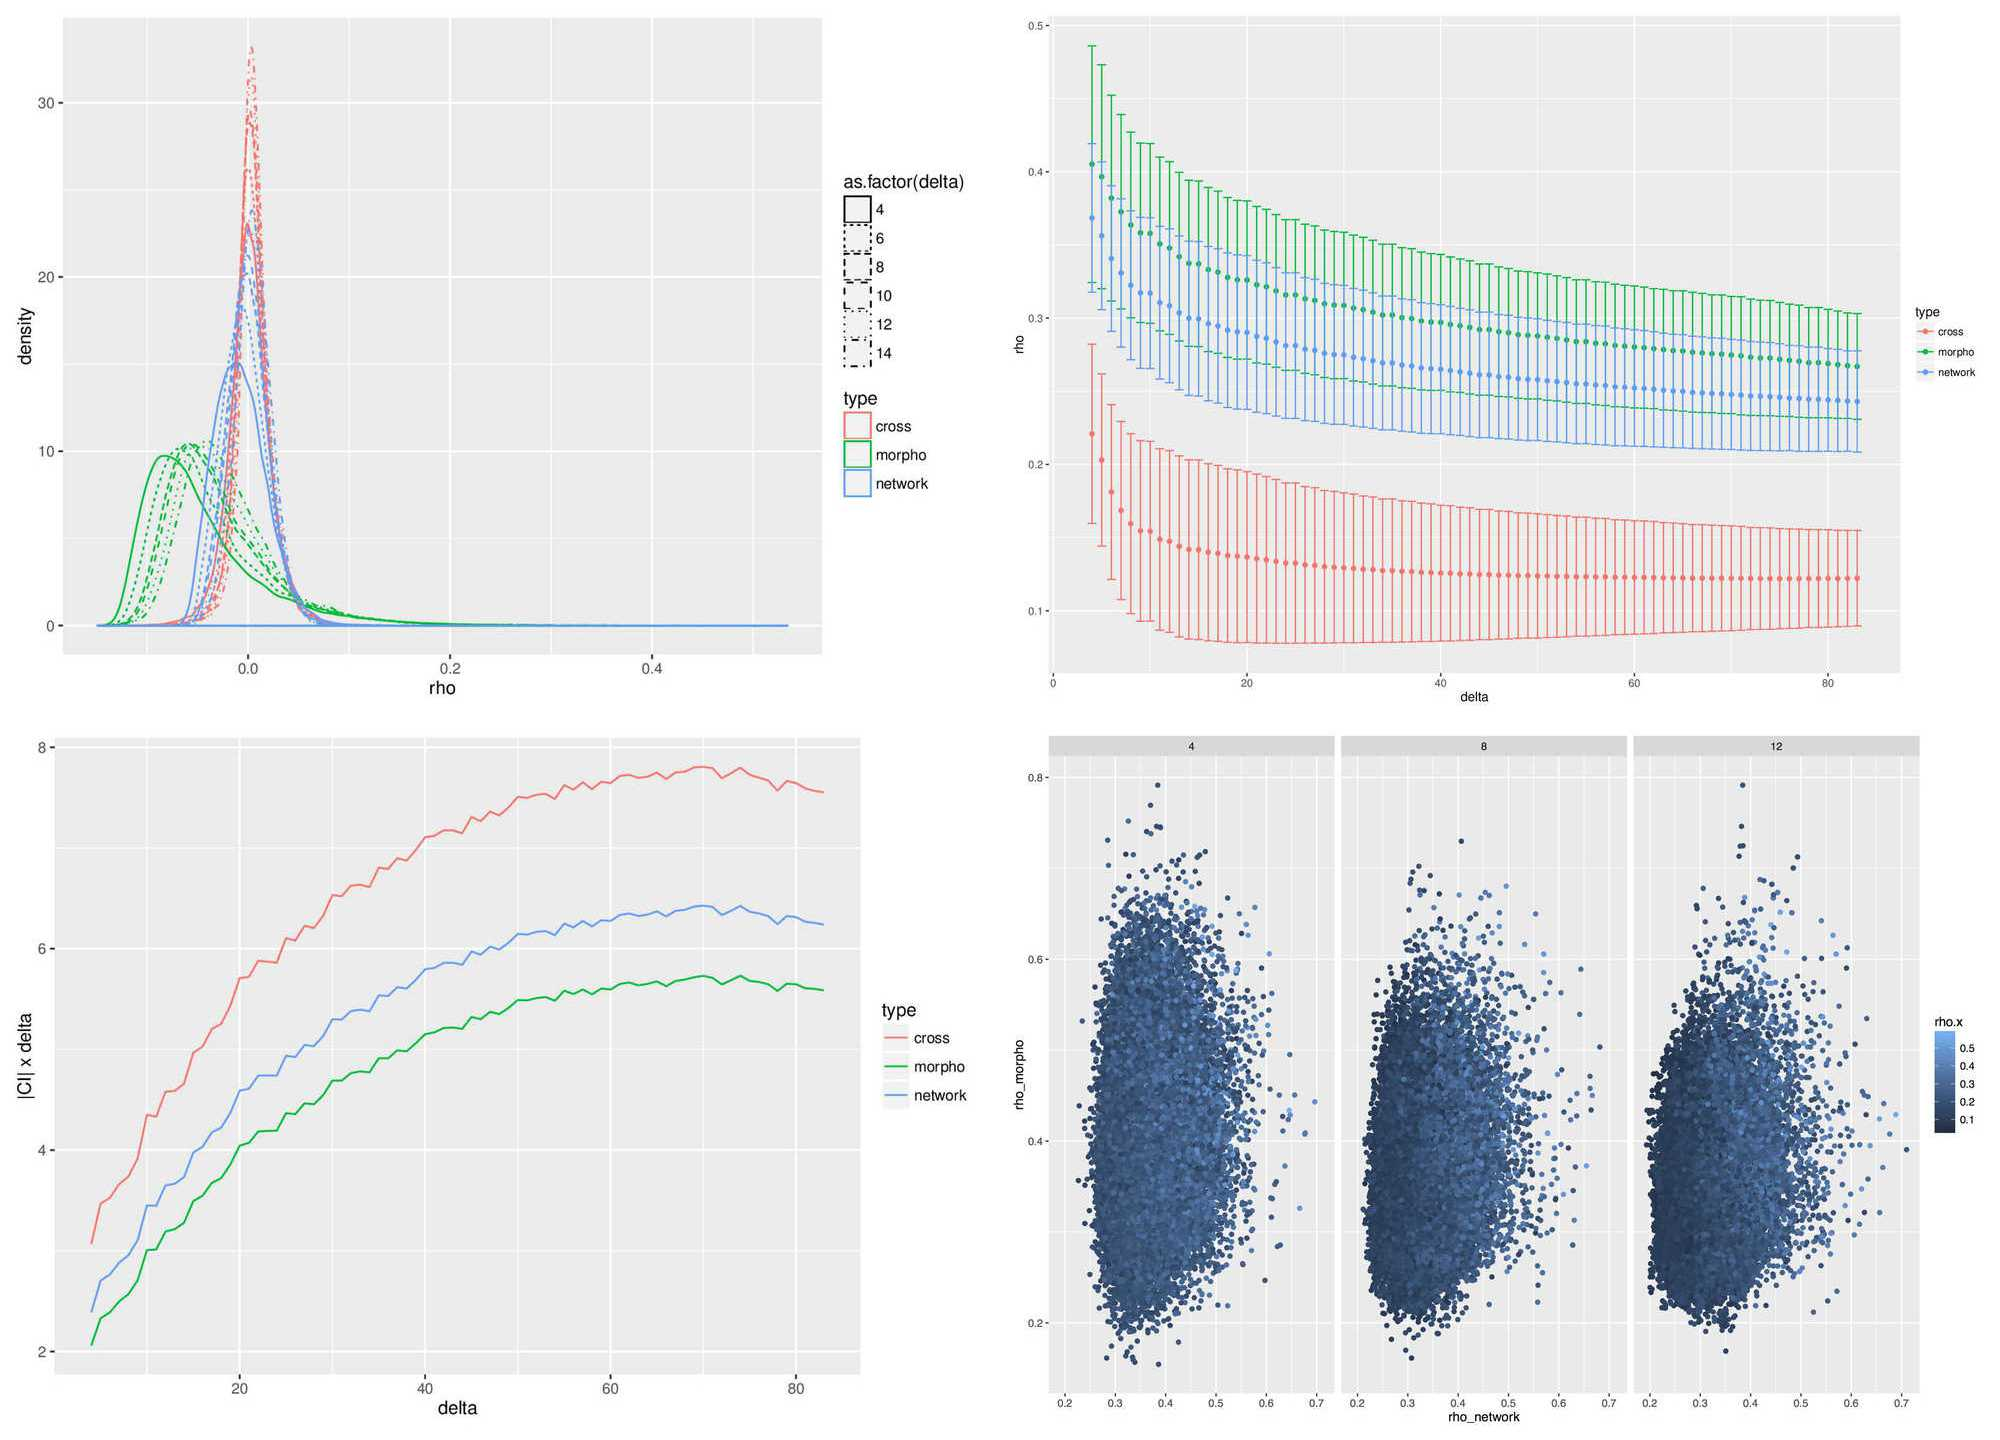
\includegraphics[width=\linewidth]{Figures/Final/4-1-3-fig-staticcorrs-corrsdistrib}
%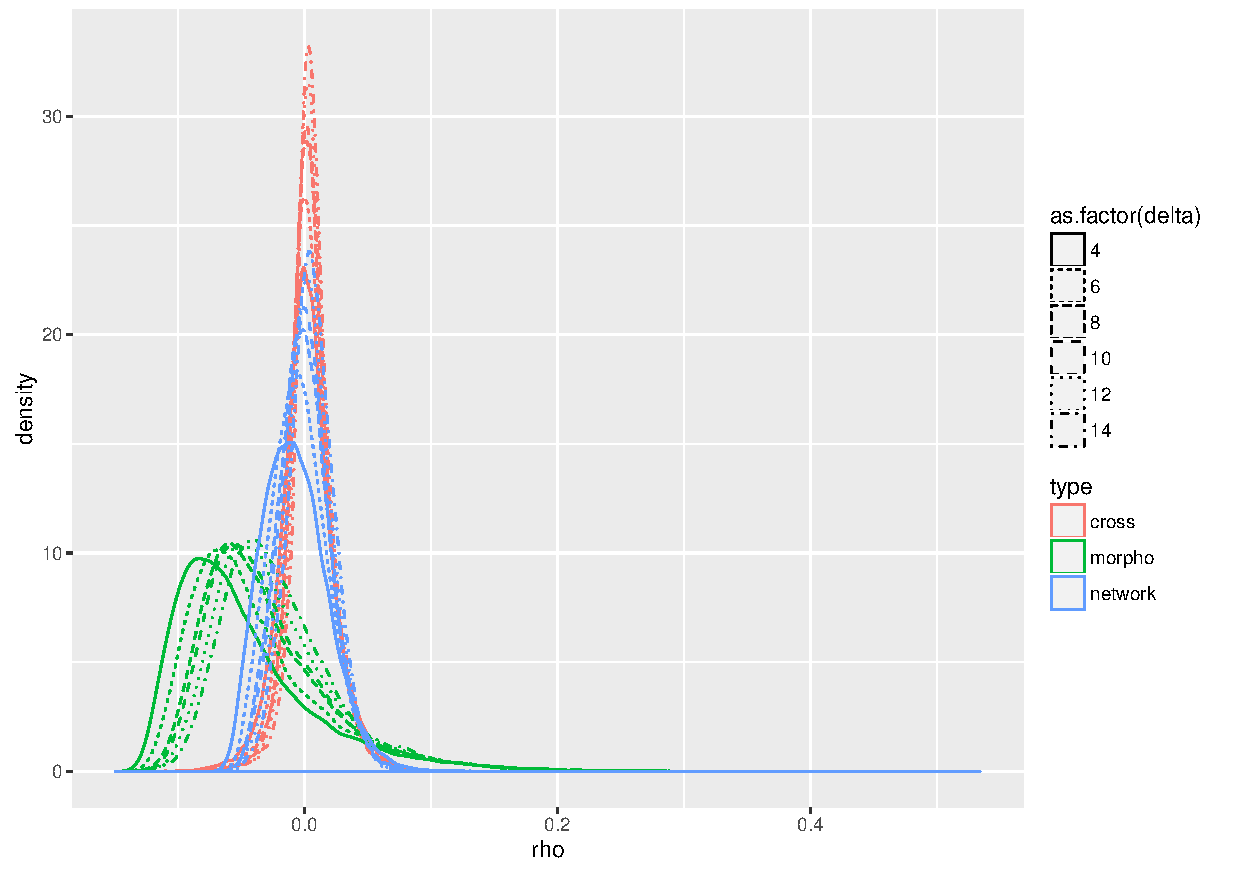
\includegraphics[width=0.48\linewidth]{Figures/StaticCorrelations/corrs-distrib_varyingdelta_bytype}
%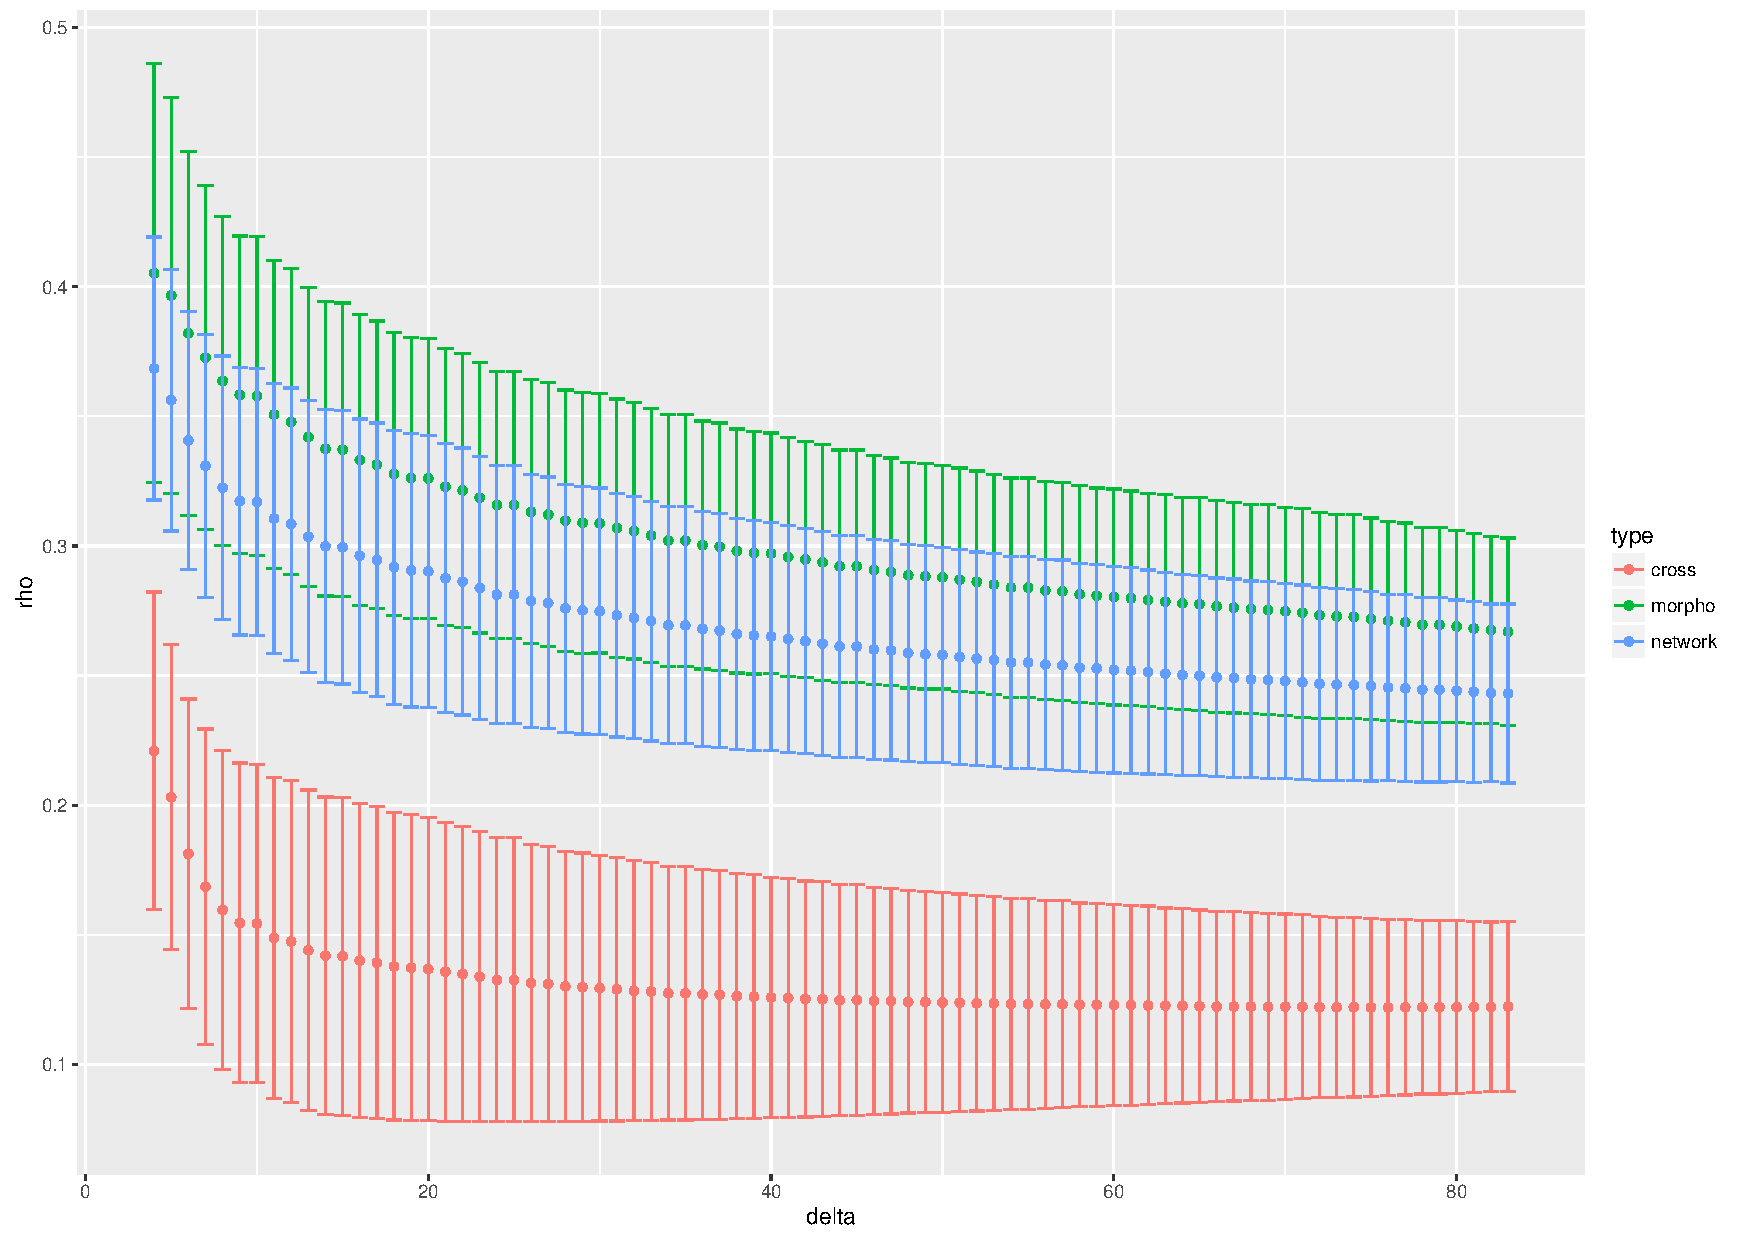
\includegraphics[width=0.48\linewidth]{Figures/StaticCorrelations/corrs-summary-meanabs_varyingdelta_bytype}\\
%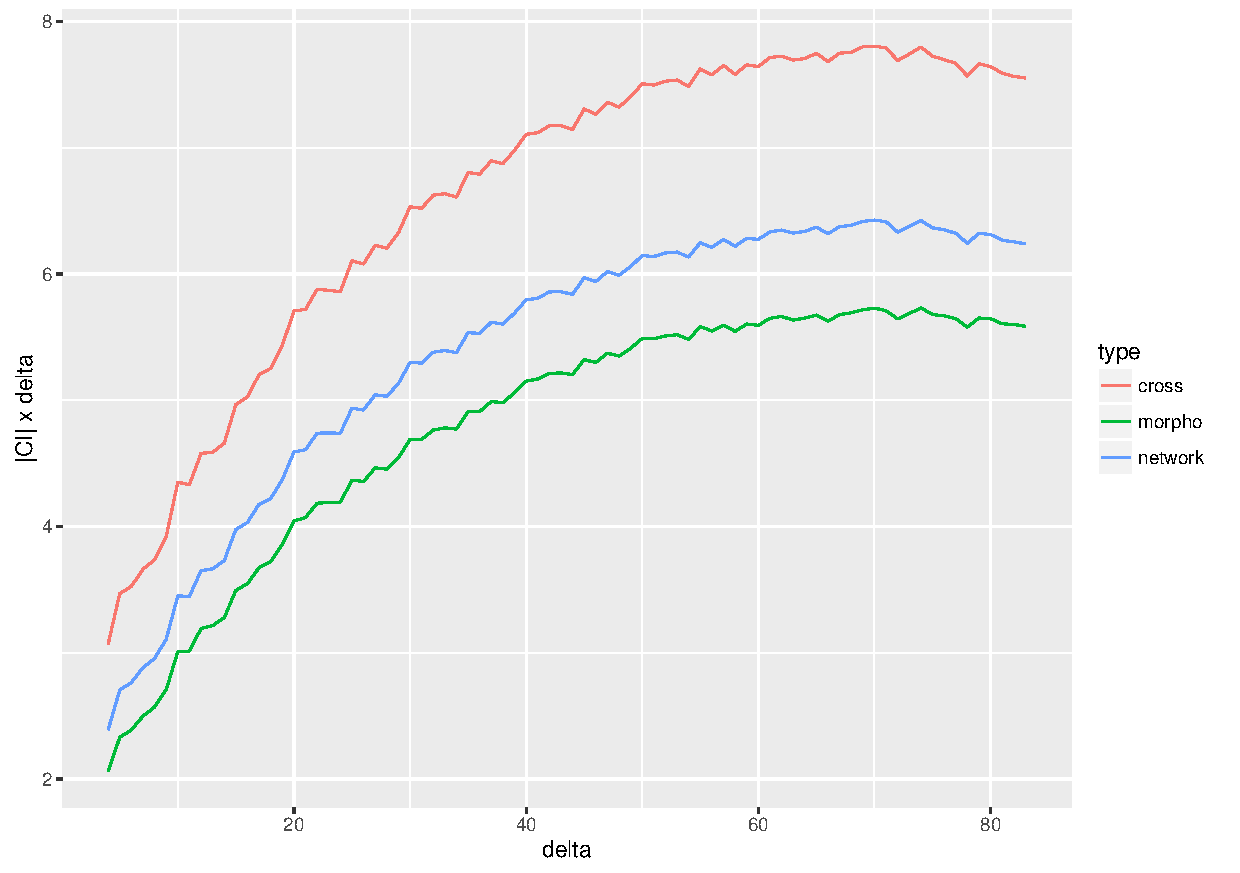
\includegraphics[width=0.48\linewidth]{Figures/StaticCorrelations/normalized_CI_delta}
%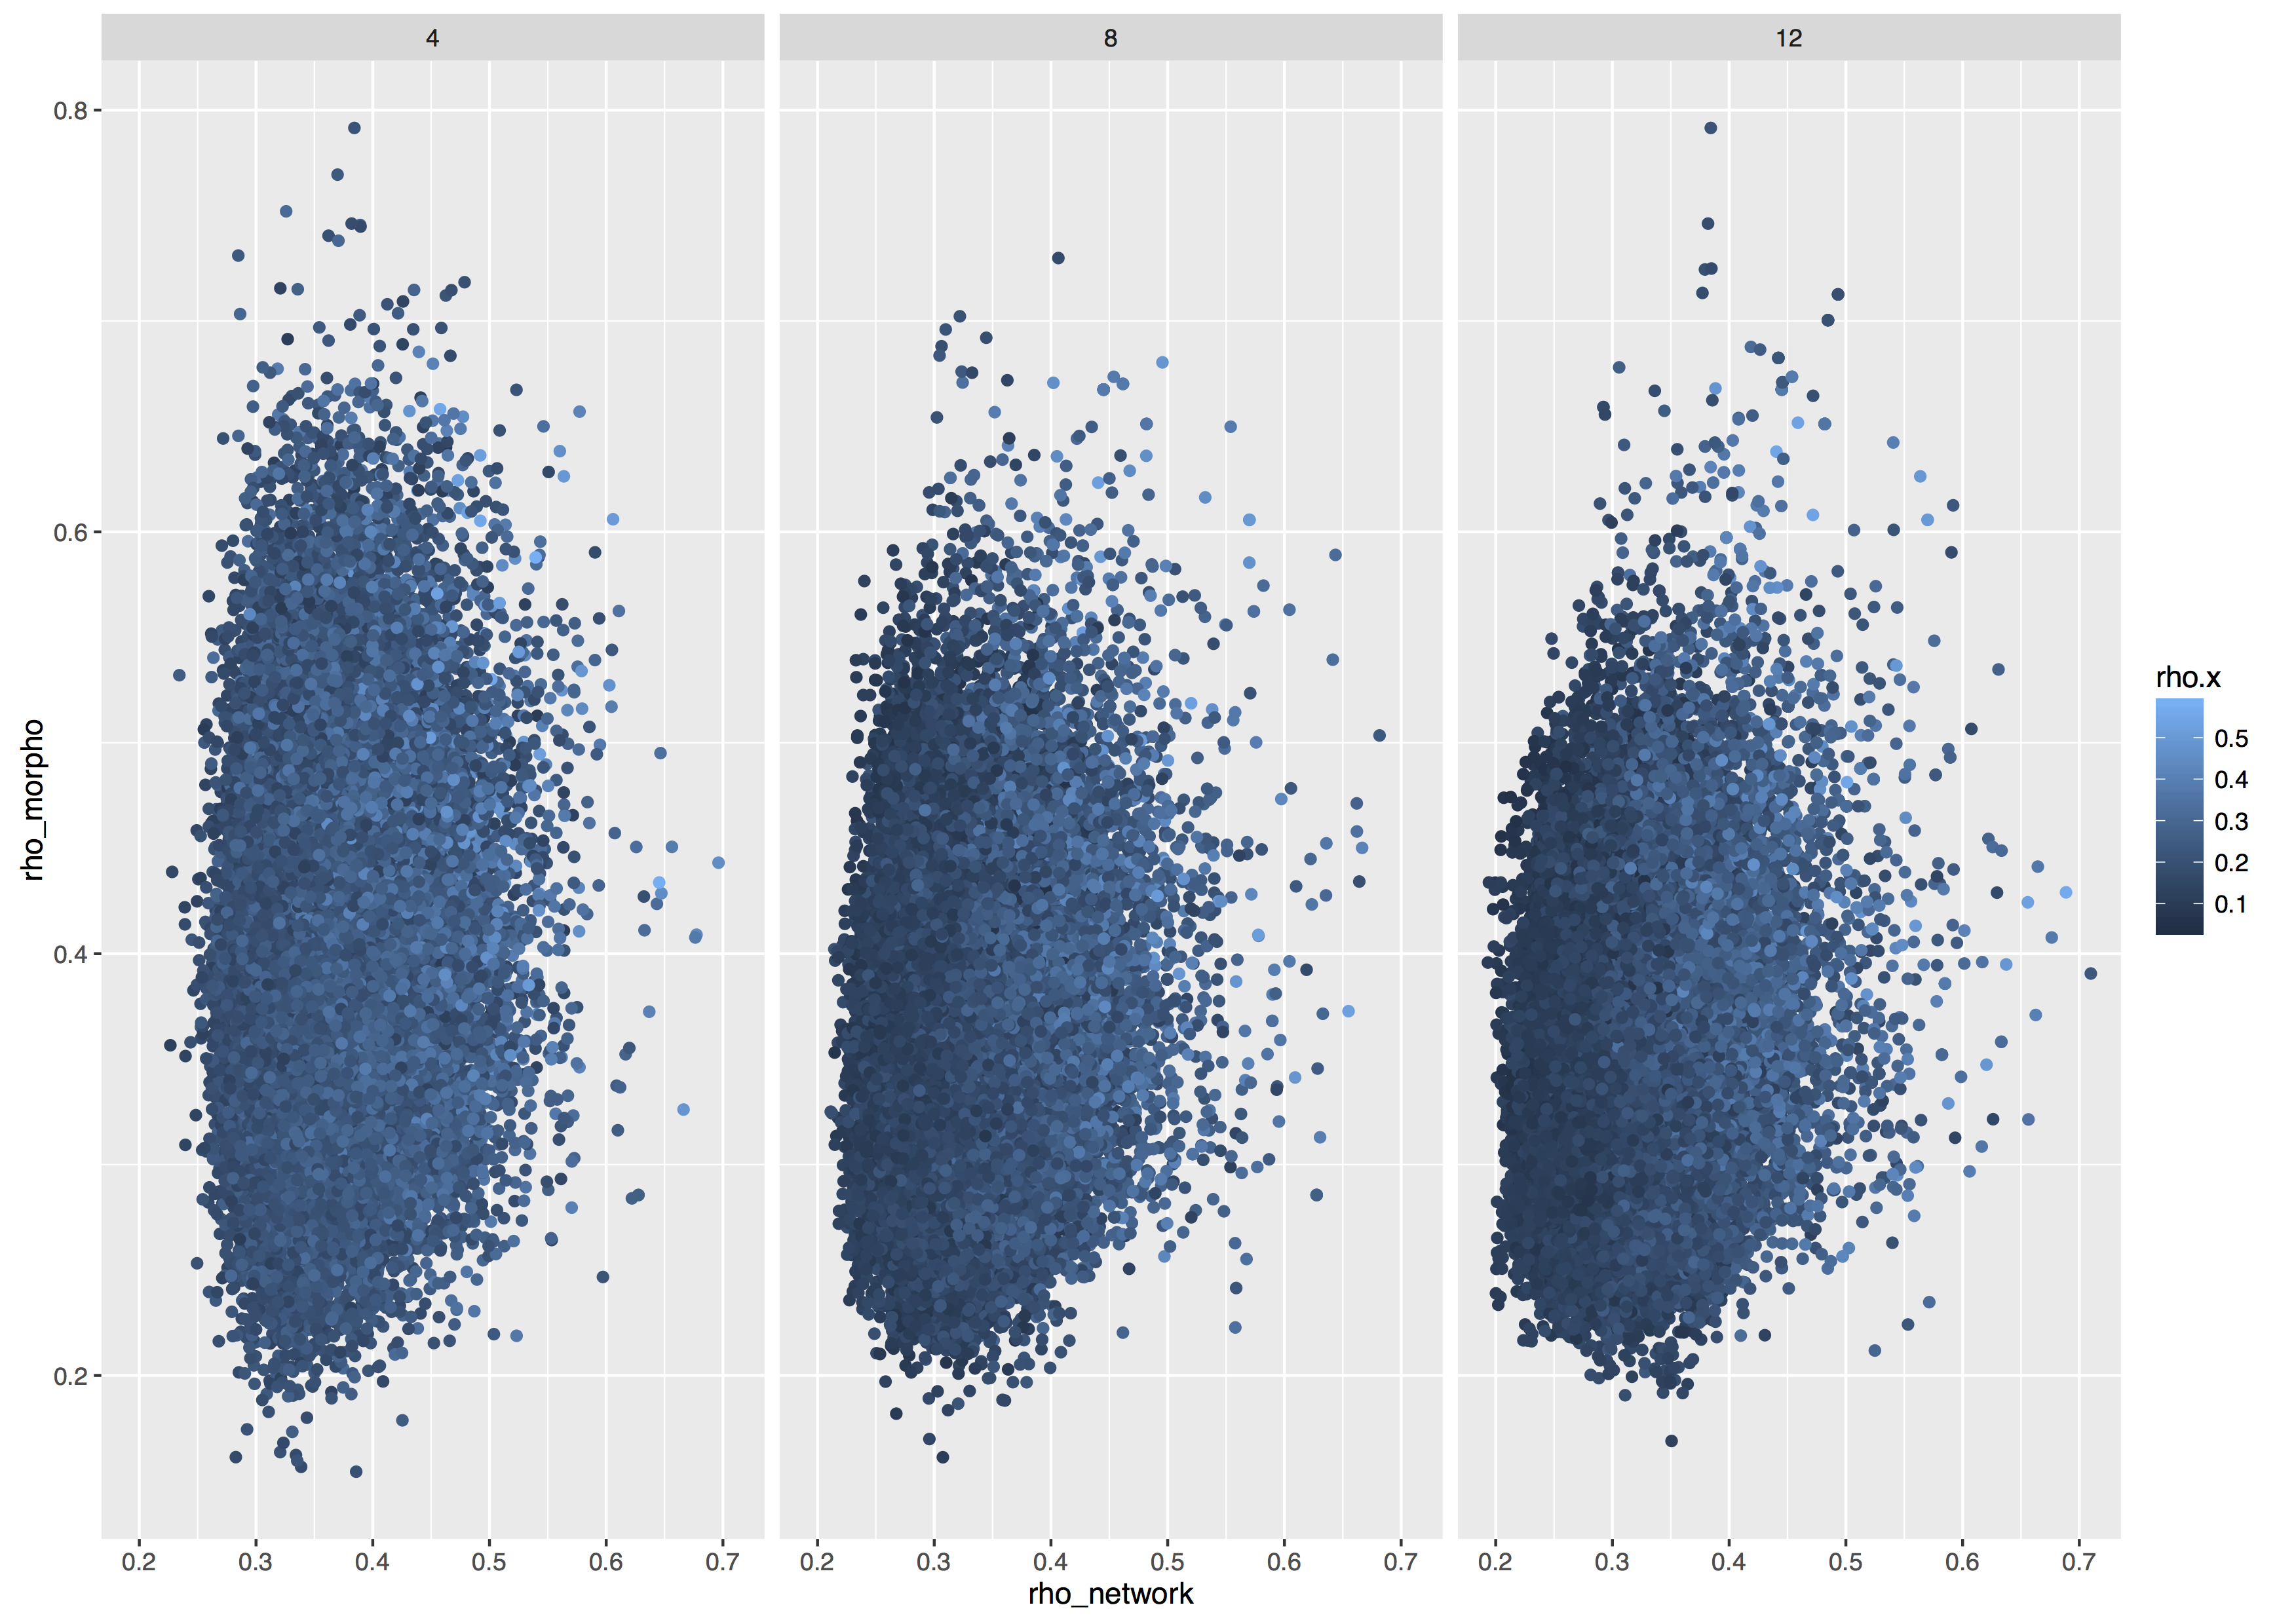
\includegraphics[width=0.48\linewidth]{Figures/StaticCorrelations/scatter_meanabs_colcross}
\caption[Variation of correlations with scale][Variation des corrélations avec l'échelle]{\textbf{Variation of correlations with scale.}\label{fig:staticcorrs:corrsdistrib}}{\textbf{Variation des corrélations avec l'échelle, pour les corrélations calculées sur l'Europe.} \textit{(Haut Gauche)} Distribution statistique des corrélations, pour les différents blocs morphologique, réseau et corrélations croisées (couleur), pour différentes valeurs de $\delta$ (type de ligne) ; \textit{(Haut Droite)} Correlations absolues moyennes et leur déviation standard, pour les différents blocs, en fonction de $\delta$ ; \textit{(Bas Gauche)} Taille de l'intervalle de confiance normalisée $\delta\cdot \left|\rho_+ - \rho -\right|$ (IC estimé par méthode de Fisher) en fonction de $\delta$ ; \textit{(Bas Droite)} Correlation absolues moyennes pour le réseau en fonction de la morphologie, niveau de couleur donnant la corrélation croisée, pour différentes valeur de $\delta$.\label{fig:staticcorrs:corrsdistrib}}
\end{figure}
%%%%%%%%%%%%%%%%%%%%%%%%




%%%%%%%%%%%%%%%%%%
\paragraph{Optimal Scales}{Echelles optimales}


\bpar{
We also compute the optimal bandwidth for a GWR PCA~\cite{harris2011geographically}. We beware to sample data accordingly to avoid local colinearity :\cite{wheeler2007diagnostic} colinearity in GWR
}{
Nous explorons d'autre part la propriété de multi-scalarité par extraction d'échelles endogène présentes dans les données. Une Analyse en Composantes Principales Géographique Pondérée (GWRPCA)~\cite{harris2011geographically} suggère des poids et importances variables dans l'espace, ce qui est cohérent avec la non-stationnarité des structures de corrélation obtenue ci-dessus. Il n'y a a priori pas de raison pour que les échelles de variation des différents indicateurs soient strictement identiques. Nous proposons donc d'extraire les échelles typiques pour les relations croisées entre forme urbaine et forme de réseau, par la méthode suivante : nous considérons un échantillon typique d'indicateurs (quatre pour chaque aspect), et pour chaque indicateur nous formulons l'ensemble des modèles linéaires possibles en fonction des indicateurs opposés (réseau pour un indicateur morphologique, morphologique pour un indicateur de réseau), visant à capturer directement l'interaction sans contrôle sur le régime de forme ou de réseau. Ces modèles sont alors ajustés par une Régression Géographique Pondérée (GWR) à portée optimale déterminée par critère d'information corrigé. Pour chaque indicateur, on retient le modèle ayant la meilleure valeur du critère d'information. Nous ajustons les modèles sur les données de la France, avec un noyau \emph{bisquare} et une portée adaptable en nombre de voisins. Les résultats sont présentés en Table~\ref{tab:staticcorrelations:gwr}. 
}

%bestmodels
%            indic             bestmodel      dist    bw        R2
%           <fctr>                <fctr>     <dbl> <dbl>     <dbl>
%1        distance  distance~networkPerf 11.609078    30 0.3145114
%2         entropy   entropy~networkPerf  8.795393    16 0.7511295
%3 meanBetweenness meanBetweenness~moran 12.294076    34 0.5776019
%4   meanCloseness   meanCloseness~moran 13.883025    44 0.2565047
%5           moran     moran~networkPerf  8.795393    16 0.4886164
%6     networkPerf   networkPerf~entropy  8.595512    15 0.8640510
%7           slope     slope~networkPerf  8.795393    16 0.6840567
%8          vcount        vcount~entropy  8.595512    15 0.8825783


%%%%%%%%%%%%%%%%%%
\begin{table}
\caption[][Relation croisées entre indicateurs de réseau et morphologiques]{}{\textbf{Relation croisées entre indicateurs de réseau et morphologiques.} Chaque relation est ajustée par une Regression Géographique Pondérée\label{tab:staticcorrelations:gwr}}
\begin{tabular}{|l|l|l|l|}
\hline
Indicateur & Modèle & Portée & Fit (R2) \\ \hline
distance & distance $\sim$ networkPerf & 11.609078 & 0.3145114 \\
entropy  & entropy $\sim$ networkPerf &  8.795393  &0.7511295 \\
meanBetweenness & meanBetweenness $\sim$ moran & 12.294076 & 0.5776019 \\
meanCloseness &  meanCloseness $\sim$ moran & 13.883025 & 0.2565047 \\
moran & moran $\sim$ networkPerf &  8.795393 & 0.4886164 \\
networkPerf & networkPerf $\sim$entropy & 8.595512  & 0.8640510 \\
slope & slope $\sim$ networkPerf & 8.795393  & 0.6840567 \\
vcount & vcount $\sim$ entropy & 8.595512  & 0.8825783 \\\hline
\end{tabular}
\end{table}
%%%%%%%%%%%%%%%%%%



%%%%%%%%%%%%%%%%%%
\subsubsection{Spatial non-stationarity and non-ergodicity}{Non-stationnarité spatiale et non-ergodicité}


\paragraph{Formalization}{Formalisation}

\bpar{
We propose to formalize our empirical findings. Let $Y_i\left[\vec{x},t\right]$ a spatio-temporal stochastic process. We showed following assumptions:
\begin{enumerate}
\item Local spatial autocorrelation is present and bounded by $l_{\rho}$ (in other words the processes are continuous in space) : at any $\vec{x}$ and $t$, $\left|\rho_{\norm{\Delta \vec{x}} < l_{\rho}}\left[Y_i (\vec{x}+\Delta \vec{x},t), Y_i (\vec{x},t) \right]\right| > 0$.
\medskip
\item Processes are locally parametrized : $Y_i = Y_i\left[\alpha_i\right]$, where $\alpha_i (\vec{x})$ varies with $l_{\alpha}$, with $l_{\alpha} \gg l_{\rho}$ and weakly locally stationary in space.
\medskip
%\item Spatial correlations between processes have a sense at an intermediate scale $l$ such that $l_{\alpha}\gg l \gg l_{\rho}$.
%\item Processes covariance stationarity times scale as $\sqrt{l}$.
%\item Local ergodicity is present at scale $l$ and dynamics are locally chaotic.
\item Processes are multi-scalar : since $\rho(\delta = \infty) > \rho (\delta = 0 )$, a necessary non-linear correction on processes spatial averages in correlation computation is present.
% add computation in supplementary materials / papers. -> later
\end{enumerate}
}{
Formalisons les conclusions empiriques obtenues. Soit $Y_i\left[\vec{x},t\right]$ un processus stochastique spatio-temporel. Nous avons alors les hypothèses suivantes :
\begin{enumerate}
\item L'autocorrelation spatiale locale existe en dessous d'une échelle minimale $l_0$ (en d'autres termes le processus est continu dans l'espace) : pour tout $\vec{x}$ et $t$, on a $\left|\rho_{\norm{\Delta \vec{x}} < l_0}\left[Y_i (\vec{x}+\Delta \vec{x},t), Y_i (\vec{x},t) \right]\right| > 0$.
\item Les processus sont localement paramétrisés : $Y_i = Y_i\left[\alpha_i\right]$, où $\alpha_i (\vec{x})$ varie à l'échelle $l_{\alpha}$, avec $l_{\alpha} \gg l_0$ et est localement stationnaire dans l'espace.
\item Les processus sont multi-scalaires : comme $\rho(\delta = \infty) > \rho (\delta = 0 )$, une nécessaire correction non-linéaire sur les moyennes spatiales des processus est présente dans le calcul des corrélations.
\end{enumerate}
}


\paragraph{On global non-ergodicity}{Sur la non-ergodicité globale}

\bpar{
Analytical Deductions
1. \textbf{Regimes of temporal correlations.} Let assume local ergodicity in $\vec{x}_0$ at scale $\delta \cdot l_0$ (reasonable with urban growth and network extension in recent times). The Ergodic theorem implies that $\exists \mathcal{T}$ such that

\[<Y_i (t) >_{\norm{\vec{x}-\vec{x}_0} < \delta\cdot l_0} = <Y_i (\vec{x}_0)>_{t\in \mathcal{T}}\] 

With spatial stationarity, $<Y_i>_{\vec{x}_0}=<Y_i>_{\vec{x}_1}$, thus $\mathcal{T}$ must be constant to be invariant by translation. By contraposition and (2), processes have different dynamical characteristics.
% if translate in a given direction, looses a small part, must be compensated by the area translated by delta (overlap), thus must be constant.
2. \textbf{Global non-ergodicity.} Let $X_k$ a partition of space into local areas. We have $<\cdot>_x = \sum_k w_k <\cdot>_{x_k} =_{(1)} \sum_k w_k <\cdot>_{\mathcal{T}_k} $. On the other hand, global ergodicity would give $<\cdot>_t = <\cdot>_{\mathcal{T}} = \sum_k w_k <\cdot>_{\mathcal{T}}$ and $\sum_k w_k \left(<\cdot>_{\mathcal{T}} - <\cdot>_{\mathcal{T}_k}\right) = 0$. Being true on each subset implies $\mathcal{T}=\mathcal{T}_k$, what contradicts (1).
}{
Nous proposons d'esquisser un lien entre les propriétés de non-stationnarité et la non-ergodicité globale des systèmes, qui est un aspect essentiel postulé par la Théorie Evolutive~\cite{pumain2012urban}, conduisant à discuter les interprétation universelles des systèmes urbains proposées par les théories du Scaling~\cite{bettencourt2007growth}. Nous suggérons que la non-stationnarité spatiale est reliée d'une part à différentes échelles de temps impliquées, et d'autre part à une non-ergodicité globale, sous l'hypothèse de stationnarité et d'ergodicité locale. Cette dernière parait raisonnable, au sens ou un régime local se manifestera de manière aléatoire sur ses différentes instances locales dans le cas d'indicateurs effectivement stochastiques à cette échelle (on pourra considérer les résultats de simulation de~\ref{sec:densitygeneration} pour se donner une idée). Empiriquement, la croissance urbaine et du réseau assez récente, rapide et étendue, laisse penser qu'on devrait être dans un cas analogue. Supposons ergodicité locale en $\vec{x}_0$ à l'échelle $\delta \cdot l_0$ à laquelle nous estimons les corrélations. Alors le théorème ergodique fournit un échantillonnage temporel $\mathcal{T}$ tel que 
\[
<Y_i (t) >_{\norm{\vec{x}-\vec{x}_0} < \delta\cdot l_0} = <Y_i (\vec{x}_0)>_{t\in \mathcal{T}}
\]
En se plaçant en un autre point $\vec{x}_1$ assez loin, la stationnarité spatiale devrait impliquer $<Y_i>_{\vec{x}_0}=<Y_i>_{\vec{x}_1}$ et $\mathcal{T}$ sera similaire pour garder invariance par translation. Par contraposition comme on a montré la non-stationnarité, les processus ont ainsi nécessairement des caractéristiques dynamiques différentes. Concernant la non-ergodicité globale, soit $X_k$ une partition de l'espace en zones locales. On a  $<\cdot>_x = \sum_k w_k <\cdot>_{x_k} = \sum_k w_k <\cdot>_{\mathcal{T}_k} $. Mais d'autre part, l'ergodicité globale impliquerait que  $<\cdot>_t = <\cdot>_{\mathcal{T}} = \sum_k w_k <\cdot>_{\mathcal{T}}$ et donc $\sum_k w_k \left(<\cdot>_{\mathcal{T}} - <\cdot>_{\mathcal{T}_k}\right) = 0$. Pour que cette relation soit vraie sur la totalité des sous-ensembles, il est nécessaire que $\mathcal{T}=\mathcal{T}_k$, ce qui contredit la propriété montrée précédemment, et le système global est nécessairement non-ergodique. Ces résultats dépendent des hypothèses théoriques, mais nous postulons qu'ils devraient rester vrais de manière empirique vu les suggestions de la Théorie Evolutive.
}






%%%%%%%%%%%%%%%%%%
\subsubsection{Discussion}{Discussion}


\paragraph{Universality}{Universalité}

\bpar{
In \cite{10.1371/journal.pone.0107042} density grids for other countries across the world are provided\footnote{available at \url{http://www.worldpop.org.uk/}}. The analysis may be repeated to other regions of the world, to compare the correlation regimes and test if urban system properties stay the same. We can expect different regimes for the United States compared to Europe for example, but the discrepancy needs still to be investigated~\cite{bretagnolle2010comparer}.
}{
Des grilles de densité de population existent pour l'ensemble des régions du monde, comme par exemple celles fournies par~\cite{10.1371/journal.pone.0107042}\footnote{disponibles à \url{http://www.worldpop.org.uk/}}. L'analyse peut être répétée pour d'autres régions, pour comparer les régimes de corrélations et tester si les propriétés des systèmes urbains restent les mêmes, en gardant à l'esprit les difficultés liées aux différences de qualité dans les données. On peut s'attendre à des régimes très différents pour les Etats-Unis en comparaison à l'Europe par exemple~\cite{bretagnolle2010comparer}, mais la différence se doit d'être étudiée quantitativement.
}



\paragraph{Further Developments}{Développements}


\bpar{
We show the regional nature of network-territories interactions, in particular the non-ergodicity of urban systems on \textbf{the interaction these components}. No direct results on time dynamics, but indirect : spatio-temporal processes do not have same speed and react/diffuse differently. Still points to explore :
\begin{itemize}
\item variable correlations areas (size and shape in space)
\item same work on cities population/train network data, which are also dynamical databases : extrapolation of ergodicity parameters ?
\item correlations of returns : link between $\rho\left[\Delta_t Y\right]$ and $\rho\left[\Delta_x Y\right]$ (more difficult : if pure local ergodicity, $\exists$ a permutation making the correspondance) % may be difficult to identify 
\item Link between $\Delta_{\delta}\rho (\delta)$ and process derivatives ?
\end{itemize}
}{
Nous avons montré empiriquement la non-stationnarité des interactions entre forme urbaine et forme de réseau, qui suggère la non-ergodicité du système urbain concernant l'interaction entre ces composantes. Nous n'extrayons pas de résultats directs sur les dynamiques par ces analyses statiques, mais pouvons postuler des résultats indirects : les processus spatio-temporels n'ont pas les mêmes vitesses et réagissent et diffusent différemment. Certains développements de cette étude serait potentiellement intéressants. La recherche d'échelle locales, c'est à dire avec une fenêtre d'estimation adaptative en taille et forme pour les corrélations, permettrait de mieux comprendre la façon dont les processus influent localement sur leur voisinage. Le critère validation de la taille resterait à déterminer : il peut s'agir comme ci-dessus de portée optimale pour des modèles locaux. La question de l'ergodicité doit également être explorée sur des bases dynamiques, en comparant les échelles de temps et d'espace d'évolution des processus, ou plus précisément les corrélations entre les variations dans le temps $\rho\left[\Delta_t Y\right]$ et celles dans l'espace $\rho\left[\Delta_x Y\right]$, mais la question de l'existence de base assez fines dans le temps paraît problématique. L'étude d'un lien entre $\Delta_{\delta}\rho (\delta)$ est les dérivées des processus est également une piste pour obtenir des informations indirectes sur la dynamique à partir des données statiques. D'autre part, la recherche de classes de processus sur lesquels il est possible d'établir directement la relation entre corrélations spatiales et corrélations temporelles, est une direction possible de recherche. On suggère par exemple en Appendice~\ref{sec:spatiotempcorrs} des cas idéaux pour lesquels un lien peut être directement obtenu, comme le cas de processus ondulatoires par exemple.
}








\stars





%
% 4.2 - Causality Regimes


\newpage



%----------------------------------------------------------------------------------------


\section[Spatio-temporal Causalities][Causalités Spatio-temporelles]{Spatio-temporal Causalities}{Causalités Spatio-temporelles}

\label{sec:causalityregimes}

%----------------------------------------------------------------------------------------




%----------------------------------------------

\bpar{This section contributes to the understanding of strongly coupled spatio-temporal processes by describing a generic method based on Granger causality. The method is validated by the robust identification of causality regimes and of their phase diagram for an urban morphogenesis model that couples network growth with density. The application to the real case study of Greater Paris transportation projects shows a link between territorial dynamics, more particularly of real estate and socio-economic, and the anticipated network growth. We finally discuss potential extensions to other temporal and spatial scales. Spatial statistics studies on dynamical relations between network and territories are relatively rare. \cite{levinson2008density} does so on London metropolitan area and identifies causalities using lagged variables, but does not disentangle relations in the sense of coupled statistical models that would isolate endogenous effects from coupling effects. study on london with temporal and spatial lag (weird use of spatial statistics). expected conclusions but does not really disentangle ?
}{
Cette section contribue à la compréhension des processus spatio-temporels fortement couplés, en proposant une méthode générique basée sur la causalité de Granger. Celle-ci est validée par l'identification robuste de régimes de causalité et de leur diagramme de phase pour un modèle de morphogenèse urbaine couplant croissance du réseau et de la densité. L'application au cas réel de l'Afrique du Sud démontre des liens évolutifs, témoins des évènements historiques entre les dynamiques démographiques territoriales et la croissance du réseau. L'utilisation de statistiques spatiales dur les relations dynamiques entre réseaux et territoires, c'est à dire cherchant à exhiber des relations de causalité, sont relativement rares. Par exemple, \cite{levinson2008density} explique pour Londres les variables de population et de connectivité au réseau par ces mêmes variables décalées dans le temps, démontrant des effets causaux réciproques. \cite{doi:10.1068/b39089} utilise des techniques similaires sur une région d'Italie sur des données historiques sur le temps long, mais modère les conclusions en rappelant l'importance des évènements historiques sur les relations estimées.
}




%%%%%%%%%%%%%%%
\subsection[Spatio-temporal Causalities][Causalités Spatio-temporelles]{A method to unveil spatio-temporal causalities}{Une méthode pour identifier des causalités spatio-temporelles}
%%%%%%%%%%%%%%%


\bpar{
}
{
L'étude des processus spatio-temporels fortement couplés implique la prise en compte d'intrications entre ceux-ci généralement difficiles à isoler. Essence même des approches par la complexité, ces interactions qui sont à l'origine du comportement émergent d'un système font sens comme objet d'étude en lui-même, et une séparation des processus paraît alors contradictoire avec une vision intégrée du système. Dans le cas des systèmes territoriaux, l'exemple des interactions entre réseaux de transport et territoires est une excellente allégorie de ce phénomène : des méthodes isolant les ``effets structurants'' d'une infrastructure développées dans les années 70~\cite{bonnafous1974methodologies} se sont révélées par la suite de l'instrumentation politique et sans fondement empirique~\cite{offner1993effets}. Le débat est toujours d'actualité puisque la question se pose toujours par exemple pour la construction de lignes à grande vitesse~\cite{crozethalshs01094554}. La réalité des processus territoriaux est en fait bien plus compliqué qu'une simple relation causale entre la mise en place d'une infrastructure et les retombées sur le développement local, mais correspond bien d'une \emph{co-évolution} complexe~\cite{bretagnolletel00459720}. Sur le temps long et à grande échelle, certains effets de renforcement des dynamiques dans les systèmes de villes par l'insertion dans les réseaux, ont été mis en valeur par l'application de la Théorie Evolutive des Villes~\cite{espacegeo2014effets}, montrant que le démêlage est toutefois possible dans certains cas par une compréhension plus globale du système. A une autre échelle, toujours concernant les relations entre réseaux et territoires, on peut citer les liens entre pratiques de mobilité, étalement urbain et localisation des ressources dans un cadre métropolitain~\cite{cerqueira2017inegalites} qui s'avèrent tout autant complexes. Ce type de problématique est bien sûr présent dans d'autres domaines : en Economie Géographique, l'exemple des liens entre innovation, impacts locaux de la connaissance et aggregation des agents économiques est une illustration typiques de processus économiques spatio-temporels présentant des causalités circulaires difficiles à démêler~\cite{audretsch1996r}. Des méthodes spécifiques sont introduites, comme l'utilisation d'instruments statistiques comme par~\cite{aghion2015innovation} dans lequel l'origine géographique des membres du Bureau du Congrès américain attribuant les subventions locales est une bonne variable instrumentale pour lier caractère innovant et inégalités des plus haut salaires, et permet de montrer que la correlation significative entre les deux est en fait une causalité de l'innovation sur les inégalités.
}


\bpar{
}{
Le couplage fort spatio-temporel implique généralement l'introduction de la notion de causalité, à laquelle la géographie s'est toujours intéressée : \cite{loi1985etude} montre que les questions fondamentales que se pose la géographie théorique récente (isolation des objects, lien entre espace et structures causales, etc.) étaient déjà présentes dans la géographie classique de Vidal. \cite{claval1985causalite} critique d'ailleurs les nouveaux déterminismes ayant émergé, notamment celui proposé par certains tenants de l'analyse systémique : dans ses débuts, cette approche héritait de la cybernétique et donc d'une vision réductionniste impliquant un déterminisme même dans une formulation probabiliste. Claval note que des travaux contemporains à son écriture devraient permettre de capturer la complexité qui fait la particularité des décisions humaines : l'école de Prigogine et la Théorie des Catastrophes de Thom. Ce point de vue est remarquablement visionnaire, puisque comme le rappelle Pumain dans \cite{pumain2003approche}, le glissement de l'analyse des systèmes à l'auto-organisation puis à la complexité a été long et progressif, et ces travaux ont été fondamentaux pour le permettre. François Durand-Dastès résume cette situation plus récemment dans \cite{durand2003geographes}, en appuyant l'importance des bifurcations et de la dépendance au chemin lors des instants initiaux de la constitution du système qu'il désigne par \emph{systèmogenèse}. % note : here we could introduce morphogenesis, form as system structure, linked to circular causalities ; topology and dynamical systems in network propagation (paper Nature Networks). Too far, but keep in mind for further work ?
Ce type de dynamique complexe implique généralement une co-évolution des composantes du système, qu'on peut interpréter comme des causalité circulaires entre processus : la question de pouvoir les identifier est donc cruciale au regard de la notion de causalité pour la géographie complexe contemporaine.
}


\bpar{
}{
Les régimes sous lesquels des identifications de causalité sont cohérentes ne sont pas identifiés de manière évidente. Ceux-ci dépendront des définition utilisées, de la même manière que les méthodes à disposition pour lesquelles nous pouvons donner quelques illustrations. \cite{liu2011discovering} propose la detection de relations spatio-temporelles entre perturbations des flots de trafic, introduisant une définition particulière de la causalité basé sur une correspondance de points extrêmes. Les algorithmes associés sont toutefois spécifiques et difficilement applicables à des types de systèmes différents. L'utilisation des correlations spatio-temporelles a été démontrée comme ayant dans certains cas un fort pouvoir prédictif pour les flots de traffic~\cite{min2011real}. Egalement dans le domaine des transports et de l'usage du sol, \cite{xie2009streetcars} applique une analyse par causalité de Granger, qu'on pourra interpréter comme une corrélation retardée, pour montrer dans un cas particulier que la croissance du réseau induit le développement urbain et est elle-même tirée par des externalités comme les habitudes de mobilité. Les neurosciences ont développé de nombreuses méthodes répondant à des problématiques similaires. \cite{luo2013spatio} définit une causalité de Granger généralisée prenant en compte la non-stationnarité et s'appliquant à des régions abstraites issues d'imagerie fonctionnelle. Ce genre de méthode est également développée en Vision par Ordinateur, comme l'illustre \cite{ke2007spatio} qui exploite les correlations spatio-temporelles de formes et de flux dans des successions d'images pour classifier et reconnaître des actions. Les applications peuvent être très concrète comme la compression de fichier videos par extrapolation des vecteurs de mouvement~\cite{chalidabhongse1997fast}. Dans l'ensemble de ces cas, l'étude des correlations spatio-temporelles rejoint les notions faibles de causalité vues précédemment. Cette contribution cherche à explorer la possibilité d'une méthode analogue pour des données spatio-temporelles présentant a priori des causalités circulaires complexes, et donc de tenter l'exercice d'équilibriste de concilier un certain niveau de simplicité et de caractère opérationnel à une prise en compte de la complexité. Nous introduisons ainsi une méthode d'analyse des correlations spatio-temporelles similaire à une causalité de Granger estimée dans le temps et l'espace, dont la robustesse est démontrée systématiquement par l'application à un modèle de simulation complexe de morphogenèse urbaine et par l'isolation de régimes de causalités distincts dans l'espace des phases du modèle. Notre contribution inclut également l'application à un cas d'étude empirique, ce qui la positionne à l'interface des domaines de la méthodologie, de la modélisation et de l'empirique.
}


\bpar{
}{
La suite de cette section est organisée de la façon suivante : le cadre générique de la méthode proposée est décrit. Nous l'appliquons ensuite à un jeu de données synthétiques afin de la valider partiellement et de tester ses potentialité, ce qui permet de l'appliquer ensuite au système urbain Sud-Africain sur le temps long. Nous discutons finalement la proximité avec d'autres méthodes existantes et des développements possibles.
}



%%%%%%%%%%%%%%%
\subsubsection{Method}{Méthode}
%%%%%%%%%%%%%%%


Nous formalisons ici de manière générique la méthode, basée sur un test similaire à la causalité de Granger, pour tenter d'identifier des relations causales dans des systèmes spatiaux. Soit $X_j(\vec{x},t)$ des processus aléatoires spatiaux unidimensionnels, se réalisant dans le temps et l'espace. On se donne un ensemble d'unités spatiales fondamentales $(u_i)$ qui peuvent être par exemple les cellules d'un raster ou un pavage quelconque de l'espace géographique. On suppose l'existence de fonctions $\Phi_{i,j}$ permettant de faire correspondre les réalisations de chaque composante aux unités spatiales, possiblement par une première agrégation locale. Une réalisation d'un système est donnée par un ensembles de trajectoires pour chaque processus $x_{i,j,t}$, et on pourra noter un ensemble de réalisations $x^{(k)}_{i,j,t}$ (accessibles dans le cas d'un modèle de simulation par exemple, ou par hypothèse de comparabilité de sous-systèmes territoriaux dans des cas réels). On suppose disposer d'un estimateur de correlation $\hat{\rho}$ s'exerçant dans le temps, l'espace et les répétitions, i.e. $\hat{\rho}\left[X,Y\right] = \hat{\mathbb{E}}_{i,t,k}\left[XY\right] - \hat{\mathbb{E}}_{i,t,k}\left[X\right]\hat{\mathbb{E}}_{i,t,k}\left[Y\right]$. Il est important de noter ici l'hypothèse de stationnarité spatiale et temporelle, qui peut toutefois aisément se relâcher dans le cas d'une stationnarité locale. D'autre part, l'autocorrelation spatiale n'est pas explicitement incluse, mais est prise en compte soit par l'agrégation initiale si l'échelle caractéristique des unités est plus grande que celle des effets de voisinage, soit par un estimateur spatial adéquat (statistiques spatiales pondérées de type \emph{GWR}~\cite{brunsdon1998geographically} par exemple). Cela nous permet de définir la correlation retardée par

\begin{equation}
\rho_{\tau}\left[X_{j_1},X_{j_2}\right] = \hat{\rho}\left[x^{(k)}_{i,j_1,t - \tau},x^{(k)}_{i,j_2,t}\right]
\end{equation}

La corrélation retardée n'est pas directement symétrique, mais on a de manière évidente $\rho_{\tau}\left[X_{j_1},X_{j_2}\right] = \rho_{-\tau}\left[X_{j_2},X_{j_1}\right]$. On applique alors cette mesure de manière simple : si $\textrm{argmax}_{\tau} \rho_{\tau}\left[X_{j_1},X_{j_2}\right]$ ou $\textrm{argmin}_{\tau} \rho_{\tau}\left[X_{j_1},X_{j_2}\right]$ sont ``clairement définis'' (les deux pouvant l'être simultanément), leur signe donnera alors le sens de la causalité entre les composantes $j_1$ et $j_2$ et leur valeur absolue le retard de propagation. Les critères de significativité dépendront du cas d'application et de l'estimateur utilisé, mais peuvent par exemple inclure la significativité du test statistique (test de Fisher dans le cas d'un estimateur de Pearson), la position des bornes d'un intervalle de confiance à un niveau donné, ou même un seuil exogène $\theta$ sur $\left|\rho_{\tau}\right|$ pour forcer un certain degré de correlation. 


% some kind of smoothing has to be introduced, either as preprocessing or as part of the optimization process (at least for first observed behavior on synthetic data. maybe it is typical of the model ?) -> similar to take into account spatial autocorrelation ? (not exactly, but close)
% - formalize mean estimator on repetitions, compare it to a direct estimator (// computation or aggregated data ?) -> OK, no need to explicit estimator in the generic part



%%%%%%%%%%%%%%%
\subsection{Synthetic data}{Données Synthétiques}



%%%%%%%%%%%%%%%
\begin{figure}%[h]
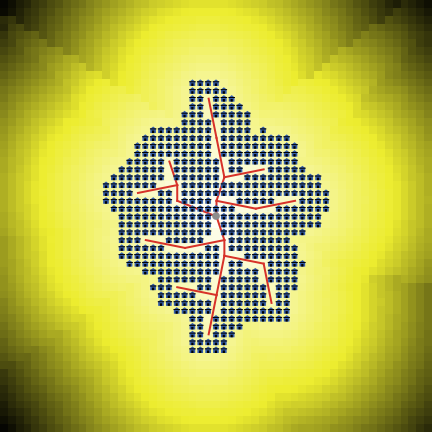
\includegraphics[width=0.32\linewidth]{Figures/CausalityRegimes/ex_60_wdens0_wroad1_wcenter1_seed272727}
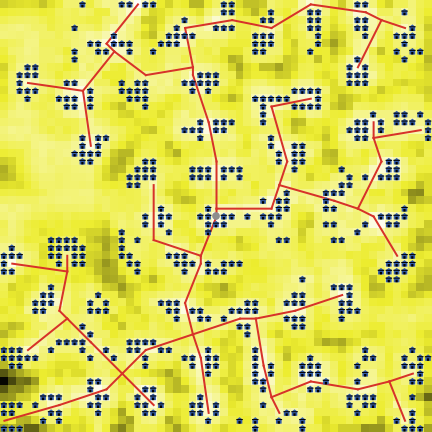
\includegraphics[width=0.32\linewidth]{Figures/CausalityRegimes/ex_60_wdens1_wroad1_wcenter0_seed272727}
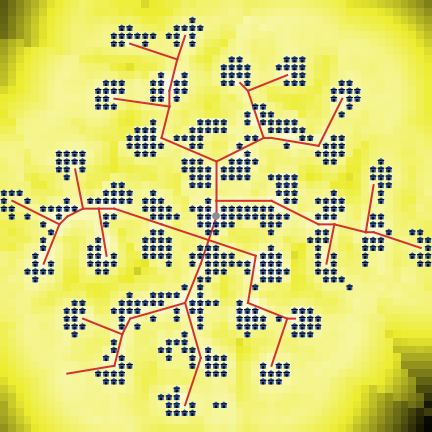
\includegraphics[width=0.32\linewidth]{Figures/CausalityRegimes/ex_60_wdens1_wroad1_wcenter1_seed272727}\\\vspace{0.2cm}
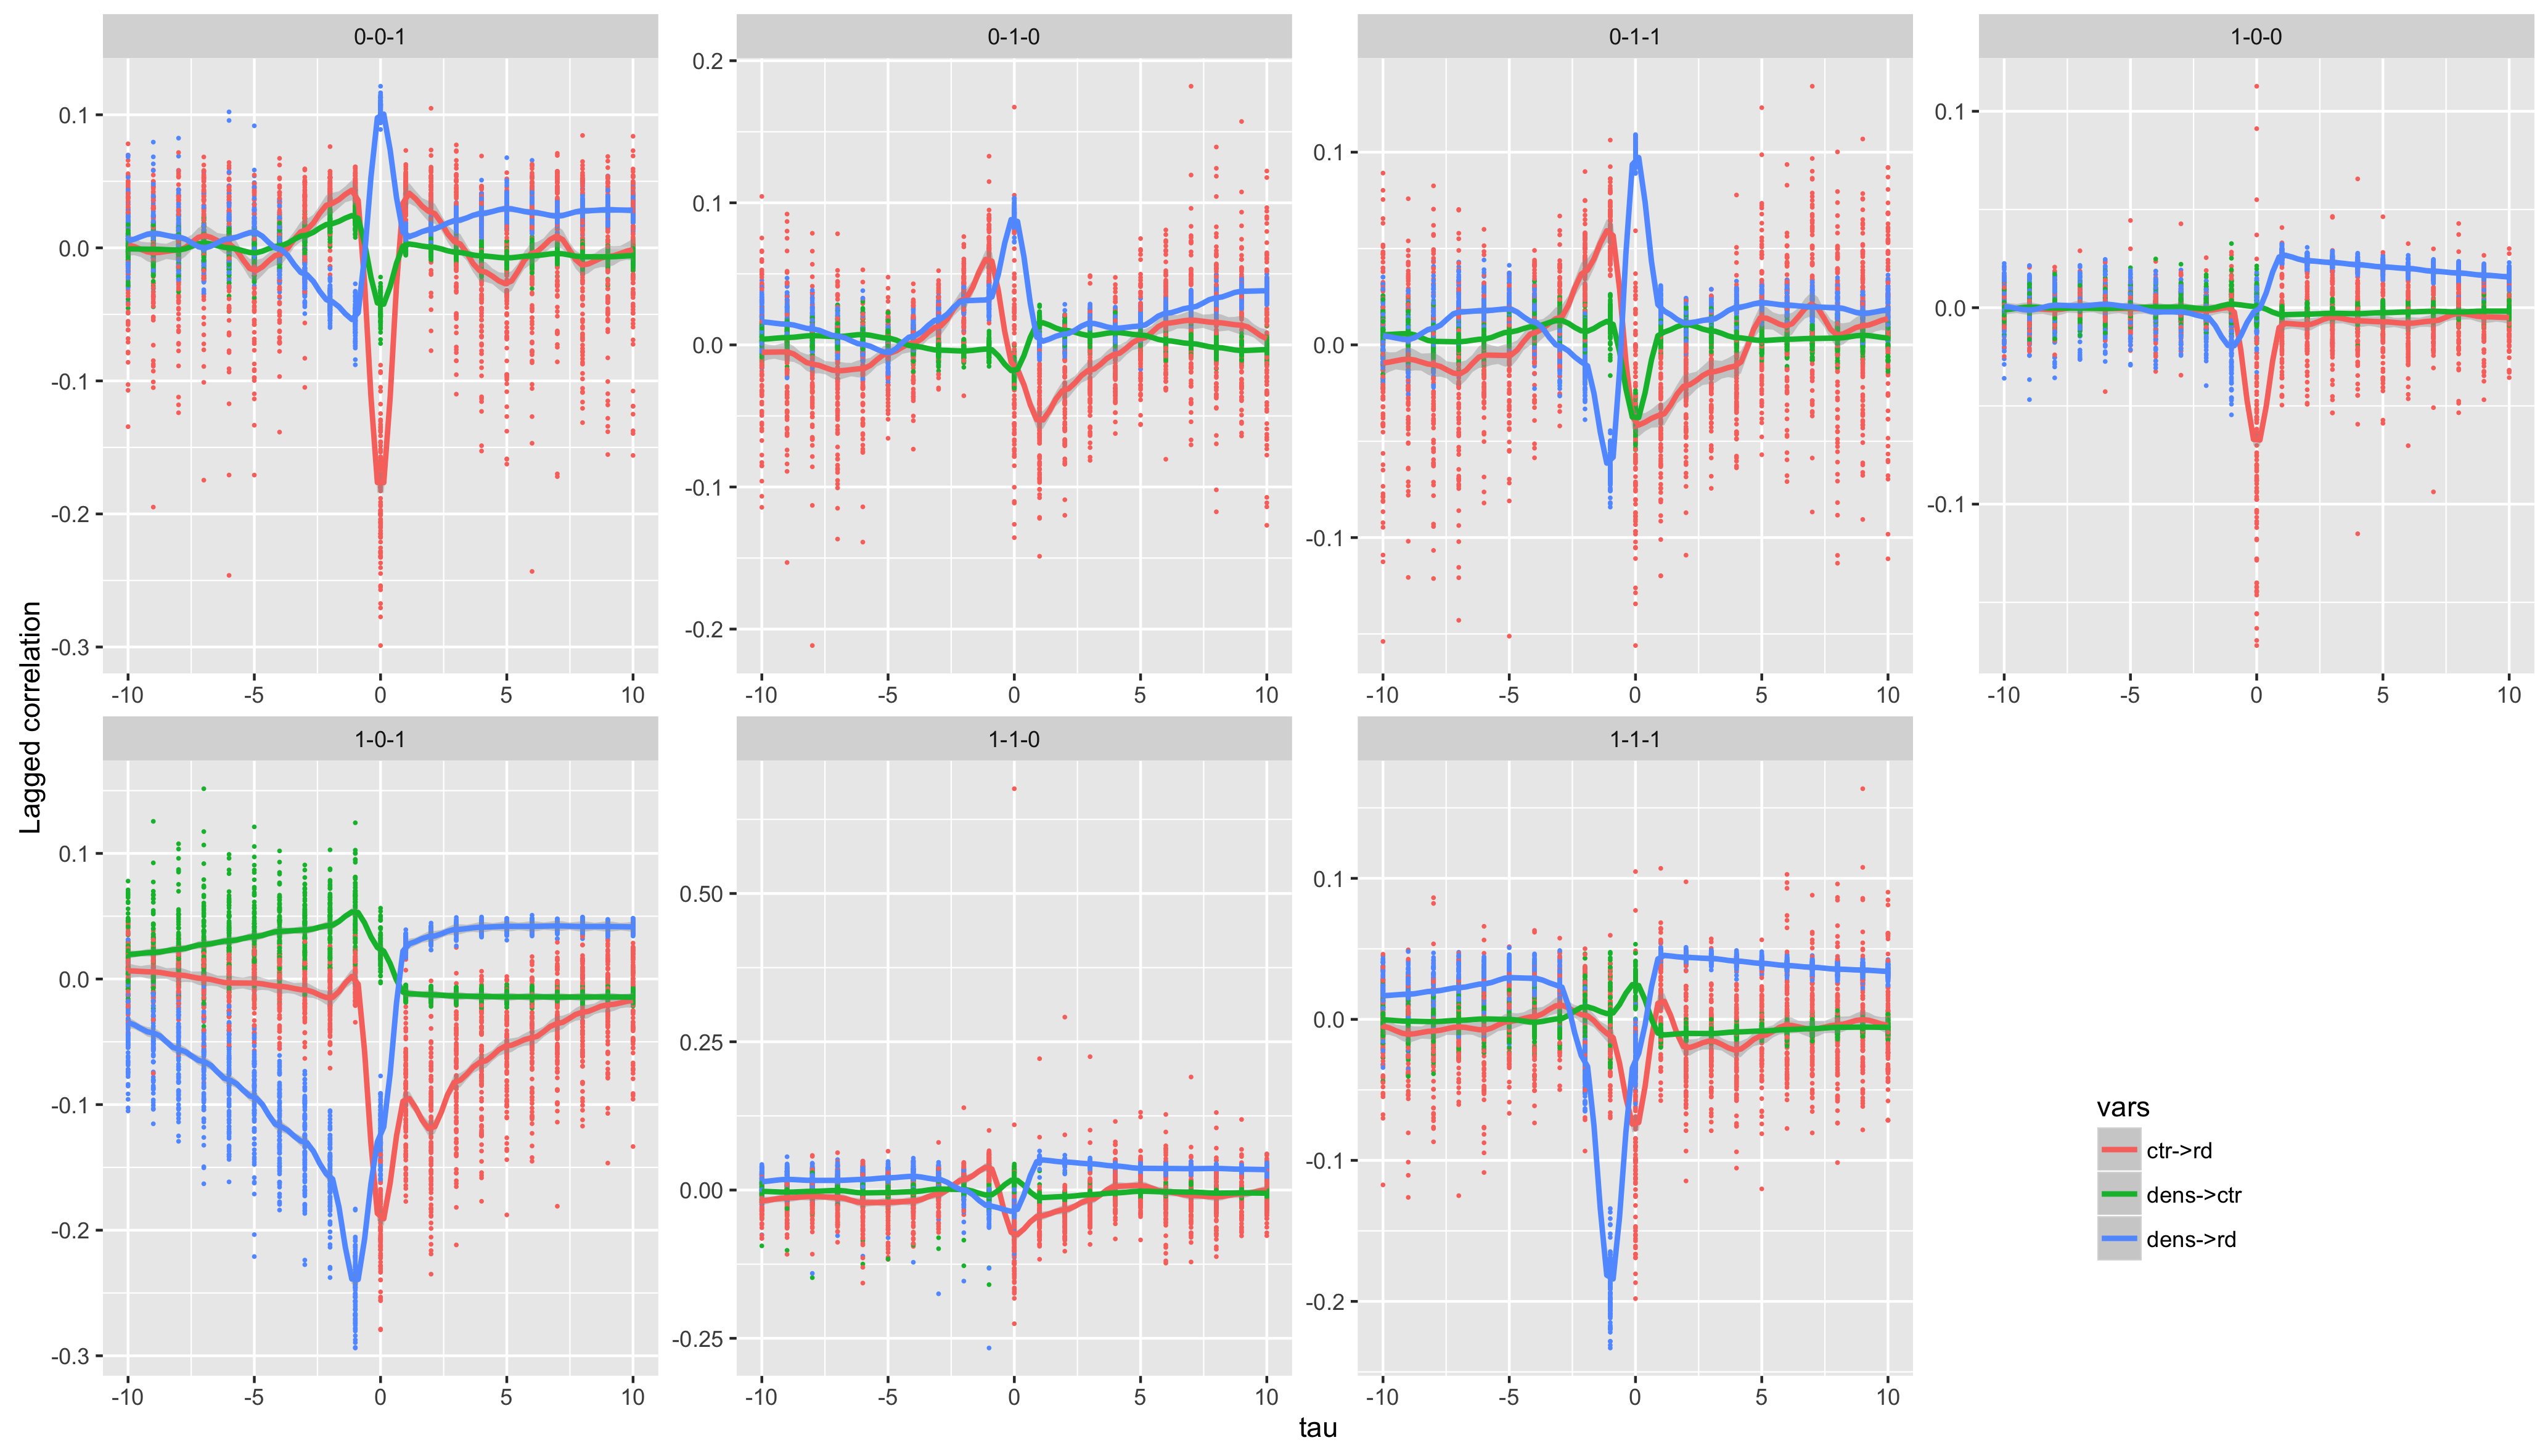
\includegraphics[width=\linewidth]{Figures/CausalityRegimes/laggedcorrs_facetextreme}
\caption[Correlation in the RBD model][Correlations dans le modèle RDB]{Correlation in the RBD model\label{fig:causalityregimes:exrdb}}{\textbf{Correlations dans le modèle RDB} \textbf{(Première ligne)} Exemples de configurations finales variées, obtenues avec $(w_{d},w_{c},w_{r})$ valant respectivement $(0,1,1)$,$(1,0,1)$, et $(1,1,1)$. \textbf{(Deuxième ligne)} Corrélations retardées, pour chaque combinaison des paramètres, en fonction du retard $\tau$. Les différentes couleurs correspondent à chaque couple de variables : distance au centre (\texttt{ctr}), densité (\texttt{dens}) et distance au réseau (\texttt{rd}). Les points montrent l'étendue sur l'ensemble des répétitions du modèle (estimateurs sur $i$ et $t$).\label{fig:causalityregimes:exrdb}}
\end{figure}
%%%%%%%%%%%%%%%



%%%%%%%%%%%%%%%
\begin{figure}%[h]
\centering
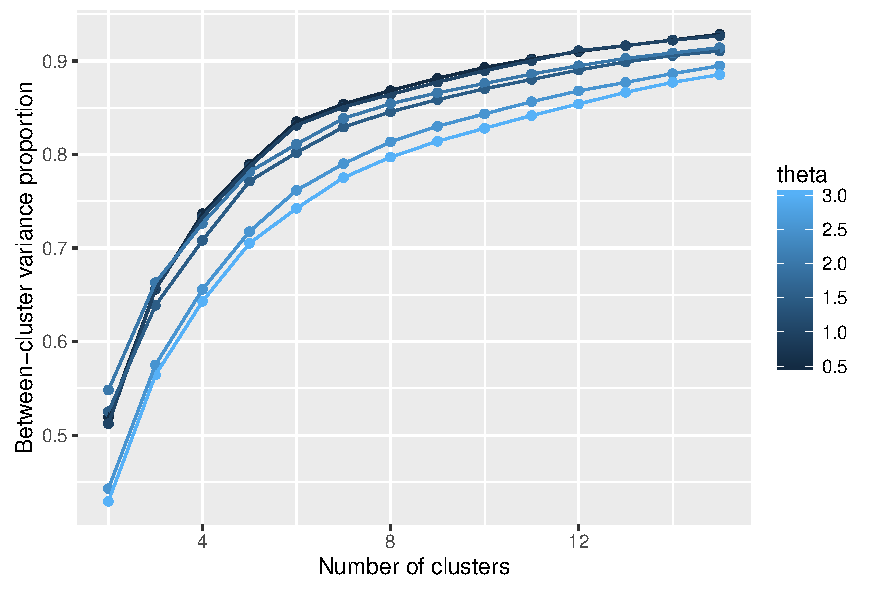
\includegraphics[width=0.49\linewidth]{Figures/CausalityRegimes/ccoef-knum_valuesFALSE_theta05-3.pdf}
\includegraphics[width=0.49\linewidth]{Figures/CausalityRegimes/dccoef-knum_valuesFALSEtheta05-3.pdf}\\
\includegraphics[width=0.4\linewidth]{Figures/CausalityRegimes/clusters-PCA-features_valuesFALSEtheta2_k6}
\includegraphics[width=0.59\linewidth]{Figures/CausalityRegimes/clusters-paramfacet_valuesFALSEtheta2_k6}\\
\includegraphics[width=\linewidth]{Figures/CausalityRegimes/clusters-centertrajs-facetclust_valuesFALSEtheta2_k6}
\caption[Identification of interaction regimes][Identification de régimes d'interactions]{Identification of interaction regimes\label{fig:causalityregimes:clustering}}{\textbf{Identification de régimes d'interactions} \textbf{(Haut Gauche)} Variance inter-cluster comme fonction du nombre de clusters. \textbf{(Haut Droite)} Dérivée de la variance inter-cluster. \textbf{(Milieu Gauche)} \emph{Features} dans un plan principal (81\% de variance expliquée par les deux premières composantes) \textbf{(Milieu Droite)} Diagramme de phase des régimes dans l'espace $(w_{d},w_{c},w_{r})$, $w_r$ variant entre les différents sous-diagrammes de $(w_{d},w_{c}$. \textbf{(Bas)} Trajectoires correspondantes des centroïdes.\label{fig:causalityregimes:clustering}}
\end{figure}
%%%%%%%%%%%%%%%




Cette méthode doit dans un premier temps être testée et partiellement validée, ce que nous proposons de faire sur des données synthétiques, méthode qui permet une connaissance plus fine des comportements des modèles~\cite{raimbault2016generation}. En écho à l'exemple des relations entre réseaux de transport et territoires qui a permis d'introduire notre problématique précédemment, nous proposons de générer des configurations urbaines stylisées dans lesquelles réseau et densité s'influencent mutuellement, et pour lesquelles les causalités ne sont pas évidents \emph{a priori} étant donné les paramètres du modèle génératif. \cite{raimbault2014hybrid} décrit et explore un modèle simple de morphogenèse urbaine (modèle RBD) répondant parfaitement à ces contraintes. En effet, les variables explicatives de la croissance urbaine, les processus d'extension du réseau et le couplage entre densité urbaine et réseau ne sont pas trop complexes. Cependant, hormis dans des cas extrêmes (par exemple lorsque la distance au centre détermine la valeur foncière uniquement, le réseau dépendra de manière causale de la densité, ou lorsque la distance au réseau seule compte, la causalité sera inversée), les régimes mixtes n'exhibent pas de causalités évidentes : c'est donc un parfait cas pour tester si la méthode est capable d'en détecter. Nous utilisons une implémentation adaptée\footnote{disponible sur le dépôt ouvert du projet à\\\texttt{https://github.com/JusteRaimbault/CityNetwork/tree/master/Models/Simple/ModelCA}} du modèle initial, permettant de capturer les valeurs des variables étudiées pour chaque patch et à chaque pas de temps et de calculer les correlations retardées entre variables au sein du modèle. Nous explorons une grille de l'espace des paramètres du modèle RBD, faisant varier les paramètres de poids de la densité, de la distance au centre et de la distance au réseau\footnote{Le modèle fonctionne de la façon suivante : une valeur des patches est déterminée par la moyenne pondérée de ces différentes variables explicatives, valeur qui détermine la croissance de nouveaux patches à l'instant suivant.}, que l'on note respectivement $(w_{d},w_{c},w_{r})$, dans $\left[0;1\right]$ avec un pas de 0.1. Les autres paramètres sont fixés à leur valeurs par défaut données par \cite{raimbault2014hybrid}. Pour chaque valeur des paramètres, nous procédons à $N=100$ répétitions ce qui est suffisant pour une bonne convergence des indicateurs. Les explorations sont effectuées via le logiciel OpenMole~\cite{reuillon2013openmole}, le grand nombre de simulations (1,330,000) nécessitant l'utilisation d'une grille de calcul. Nous calculons sur l'ensemble des patches les corrélations retardées par estimateur de Pearson non biaisé entre les variations des variables suivantes\footnote{Calculer les corrélations sur les variables directement n'a pas de sens puisque leur valeur n'en a pas en absolu.} : densité locale, distance au centre et distance au réseau. La Fig.~\ref{fig:causalityregimes:exrdb} montre le comportement de $\rho_{\tau}$ pour chaque couple de variable (non dirigé, $\tau$ prenant des valeurs négatives et positives), pour les combinaisons des valeurs extrêmes des paramètres. On peut voir déjà différents régimes émerger : par exemple, $(1,0,1)$ conduit à une causalité de la densité sur la distance au centre avec un retard 1, et une causalité négative de la densité sur la distance au réseau avec le même retard, tandis que distance au centre et au réseau sont corrélés de manière synchrone. Afin d'étudier ces comportements de manière systématique, nous proposons d'identifier des régimes de manière endogène, en procédant à un apprentissage non-supervisé. Nous appliquons une classification des \emph{k-means}, robuste à la stochasticité (5000 répétitions), avec les points caractéristiques (\emph{features}) suivants : pour chaque couple de variable, $\textrm{argmax}_{\tau} \rho_{\tau}$ et $\textrm{argmin}_{\tau} \rho_{\tau}$ si la valeur correspondante est telle que $\frac{\rho_{\tau}-\bar{\rho}_{\tau}}{\left|\bar{\rho}_{\tau}\right|} > \theta$ avec $\theta$ paramètre de seuil, 0 sinon. L'inclusion des \emph{features} supplémentaires des valeurs de $\rho_{\tau}$ n'influence pas significativement les résultats, celles-ci n'ont pas été prises en compte pour réduire la dimension. Le choix du nombre de clusters $k$ est en général épineux dans ce genre de problème~\cite{hamerly2003learning}, dans notre cas le système possède une structure agréable : les courbes de la proportion de variance inter-cluster et de sa dérivée en Fig.~\ref{fig:causalityregimes:clustering}, en fonction de $k$ pour différentes valeurs de $\theta$, présentent une transition pour $\theta = 2$, ce qui donne pour cette courbe une rupture à $k=5$. Un examen visuel des clusters dans un plan principal confirme la bonne qualité de la classification pour ces valeurs. Une classe correspond alors à un \emph{régime de causalité}, dont nous pouvons représenter le diagramme de phase en fonction des paramètres du modèle, ainsi que les trajectoires des centres des clusters (calculées comme barycentre dans l'espace complet initial) en Fig.~\ref{fig:clustering}. Le comportement obtenu est particulièrement intéressant : les régions du diagramme correspondant aux régimes sont clairement délimitées et connexes. Par exemple, on observe l'émergence du régime 6 où la distance au réseau cause fortement la densité de manière négative, mais la distance au centre cause la distance au réseau, régime dont l'étendu maximale sur $(w_d,w_r)$ est pour une valeur intermédiaire $w_r=0.7$. Ainsi, pour maximiser l'impact du réseau sur la densité, il ne faut pas maximiser le poids correspondant, ce qui peut paraître contre-intuitif en premier abord : cela illustre l'intérêt de la méthode dans le cas de relations circulaires difficiles à démêler a priori. Le régime 5, où la distance au réseau influence la densité de la même manière, mais la relation entre distance au centre et route est inversée, est tout aussi intéressant, et est prédominant dans les faibles $w_r$. Le régime 1, extrême, correspond à une situation isolée dans laquelle la distance au centre n'importe pas : cet aspect domine alors totalement les autres processus d'interaction entre densité et réseau. Cette application sur données synthétique démontre ainsi d'une part la robustesse de la méthode vu la cohérence des régimes obtenus, et constitue aussi une qualification beaucoup plus précise des comportements du modèle que celle réalisée dans l'article initial. Dans ce cas précis, il peut s'agir d'un instrument de connaissance des relations entre réseaux et territoires en lui-même, permettant le test d'hypothèses ou la comparaison de processus dans le modèle stylisé.



















%--------------------------------------------------------









%%%%%%%%%%%%%%%%%%%%%%%
\subsection{Network-territory relations in South Africa}{Relations Réseaux-territoires en Afrique du Sud}



\bpar{
We assum that territorial dynamics and network dynamics responded differently to these. We expect to learn from these project informations on interactions at long time scale and large spatial scale, in a very particular context of constrained growth.
}{
Nous démontrons à présent les potentialités de notre méthode sur des données géo-historiques sur le temps long, pour le cas du réseau ferré en Afrique du Sud au cours du 20ème siècle. En faisant l'hypothèse que les territoires et les réseaux réagissent différemment aux événements historiques, les motifs de causalité devraient informer sur leur relations sur le temps long.
}


\subsubsection{Context}{Contexte}


\bpar{
Transportation Networks can be leveraged as a powerful socio-economic control tool, with even more significant outcomes when it percolates to their interaction with territories. The case of South Africa is an accurate illustration, as \cite{baffi:tel-01389347} shows that during apartheid railway network planning was used as a racial segregation tool by shaping strongly constrained mobility and accessibility patterns. In particular, it is shown qualitatively that dynamics between territories and networks profoundly changed at the end of the apartheid, transforming a tool of planed segregation (network shaped was optimized to minimize unwanted accessibility) into an integration tool thanks to recent changes in network topology patterns. We propose to investigate the potential \emph{structural} properties of this historical process, by focusing on dynamical patterns of interactions between the railway network and city growth. More precisely, we try to establish if the segregative planning policies did actually modify the trajectory of the coupled system, what would correspond to deeper and wider impacts. 
}{
Les réseaux de transport peuvent être utilisés comme un puissant outil de contrôle socio-économique, avec des effets encore plus significatifs lorsque ceux-ci perturbent les relations avec les territoires. Le cas de l'Afrique du Sud est une illustration pertinente, puisque \noun{Baffi} montre dans~\cite{baffi:tel-01389347} que lors de l'apartheid la planification du réseau ferré était utilisée comme un outil de ségrégation raciale par l'établissements de motifs de mobilité et d'accessibilité fortement contraints. En particulier, il est montré qualitativement que les dynamiques entre réseaux et territoires ont profondément changé à la fin de l'apartheid, transformant un outil de ségrégation planifiée (une forme de réseau optimisée pour minimisée une accessibilité non désirée) en un outil d'intégration grâce à des changement récents dans la topologie du réseau. Nous étudions ici les potentielles propriétés \emph{structurelles} de ce processus historique, en se concentrant sur les motifs dynamiques des interactions entre le réseau ferré et la croissance des villes. Plus précisément, nous essayons d'établir si les politiques de planification ségrégatives ont effectivement modifié la trajectoire du système couplé, ce qui correspondrait à des impacts plus larges et profonds que leurs effets immédiats.
}





\subsubsection{Results}{Résultats}


\paragraph{Data}{Données}


\bpar{
We use a comprehensive database covering the full South African railway network from 1880 to 2000 with opening and closing dates for each station and link, together with a city database spanning from 1911 to 1991 for which consistent ontologies for urban areas have been ensured. These database are described by~\cite{baffi:tel-01389347}, but they are not open so we make available only the aggregated data we used in the analysis.
}{
Nous utilisons une base de données complète couvrant l'ensemble du réseau ferré Sud-Africain de 1880 à 2000 avec les dates d'ouverture et de fermeture pour chaque station et liaison, couplée à une base de données pour les villes s'étendant de 1911 à 1991 pour laquelle des ontologies consistantes pour les aires urbaines ont été assurées. Ces bases de données sont décrites par~\cite{baffi:tel-01389347}, mais ne sont pas ouvertes, nous mettons ainsi à disposition uniquement les données agrégées utilisées dans l'analyse.
}



\paragraph{Network Measures}{Mesures de réseau}

\bpar{
First, a dynamical study of network measures seem to confirm the hypothesis: a trend rupture in closeness centrality (defined for a node as the average travel time to other nodes) at a roughly constant network size evolution, at a date corresponding to the beginning of official segregative policies, suggests that the planning process after this date had in the best case no global effect on network performance, and in the worst case had intended negative effects on accessibility with the aim to physically segregate more.
}{
Une analyse préliminaire consiste à regarder l'évolution dynamique des mesures de réseau, celles-ci pouvant témoigner de ruptures dans les propriétés structurelles du réseau et donc de mutations historiques profondes. L'évolution de certaines propriétés du réseau, comme les distributions de la centralité ou de l'accessibilité, peut témoigner l'existence d'une planification les ayant influencées. Nous montrons en Figure~\ref{fig:causalityregimes:network} l'évolution des mesures de réseau dans le temps, correspondant aux mesures les plus basiques de celles définies en~\ref{sec:staticcorrelations}. La centralité de proximité, que nous définissons comme le temps moyen de trajet vers les autres noeuds, présente un comportement intéressant. En effet, la taille du réseau et les valeurs moyennes des centralités présentent un comportement concordant, qui correspond à l'expansion initiale du réseau. Par contre, la tendance de la hiérarchie de la centralité de proximité à se réduire est soudainement rompue à la date correspondant à l'officialisation des politiques ségrégatives en 1951, alors que taille et forme géométrique globale du réseau, traduite par l'efficience, restent constants. Ainsi, la planification après cette date a dans le meilleur des cas eu aucun effet sur cette propriété, dans le pire des cas est en effet responsable de cette rupture de tendance, c'est à dire a eu les effets escomptés sur l'accessibilité, dans le but d'empêcher la diminution de la ségrégation, puisque plus la hiérarchie est faible plus le réseau est égalitaire.
}


%%%%%%%%%%%%%%
\begin{figure}[h!]
\includegraphics[width=0.42\linewidth]{Figures/CausalityRegimes/nw_nwSize}
\includegraphics[width=0.47\linewidth]{Figures/CausalityRegimes/nw_meanCentralities}\\
\includegraphics[width=0.48\linewidth]{Figures/CausalityRegimes/nw_hierarchies}
\includegraphics[width=0.41\linewidth]{Figures/CausalityRegimes/nw_efficiency}
\caption[Evolution of network measures][Evolution des mesures de réseau]{\label{fig:causalityregimes:network}}{\textbf{Evolution des mesures de réseau.} On calcule pour l'ensemble des dates les mesures basiques de réseau : taille, centralités résumées par leur hiérarchie et leur moyenne, efficience. Les centralités sont normalisées pour comparaison de leur variation respective ($\max \bar{bw} = 0.07$, $\max \bar{cl} = 1.5e-4$).\label{fig:causalityregimes:network}}
\end{figure}
%%%%%%%%%%%%%%



\paragraph{Causality patterns}{Motifs de causalité}


\bpar{
We then turn to dynamical interactions between the railway network and city growth. For that, we study Granger causalities, in the large sense of correlations between lagged variables, estimated between cities growth rates and accessibility differentials due to network growth, for all cities and urban areas having a connection to the network.
We test both travel-time and population weighted accessibilities, for varying values of distance decay parameter. Lagged correlations are fitted on varying length time windows, to test for potentially varying stationarity scales. Results are shown in Figure~\ref{fig:causalityregimes:sudafcorrs}. We find that results are significant with travel-time accessibility only, autocorrelation dominating with weighted accessibility. A time-window of 30 years appears to be a good compromise between the number of significant correlations ($p<0.1$ for a Fisher test) and the absolute correlation level across all lags and distance decays, what should correspond roughly to the time-stationarity scale of the system. We observe furthermore a phase transition when distance decay increases, revealing the shift between the spatial scale of urban areas and the scale of the country, what gives local spatial stationarity scale. We obtain therethrough clear causality patterns, namely an inversion of the Granger causality (lagged correlation up to 0.5 for several values of distance decay), from accessibility causing population growth with a lag of 10-20 years before the apartheid (1948), to the opposite after the apartheid (lag 20 years). We interpret these as \emph{Structural segregation}, i.e. a significant impact of planning policies on dynamics of interactions between networks and territories. Indeed, the first regime corresponds to direct effect of transportation on migrations in a free context in opposition to the second one.
}{
Nous examinons à présent les interactions dynamiques entre le réseau ferré et la croissance urbaine. Pour cela, nous appliquons la méthode développée dans la première partie, qui consiste à l'étude des causalités de Granger, au sens large des corrélations entre les variables retardées, estimées entre les taux de croissance des villes et les différentiels d'accessibilité dus à la croissance du réseau, pour toutes les villes ou aires urbaines ayant une connection au réseau. Nous testons à la fois l'accessibilité en terme de distance et pondérée par la population à l'origine et aux deux extrémités. Si $P_i$ sont les populations, $d_{ij}$ la matrice de distance dans le réseau, l'accessibilité de $i$ sera donnée par $Z_i = w_i \sum_j w_j \exp \left(- d_{ij} / d_0 \right)$ où $d_0$ est le paramètre de décroissance et les poids $w_i$ sont $1/N$ ou $P_i / \sum_j P_j$ selon la modalité. Nous faisons varier les valeurs de $d_0$ pour prendre en compte les relations à différentes échelles spatiales. De plus les corrélations retardées sont estimées sur des fenêtres temporelles de taille variable $T_W$, pour tester différentes échelles de stationnarité temporelles potentielles. Les résultats des estimations sont montrés en Figure~\ref{fig:causalityregimes:sudafcorrs}. Nous obtenons des résultats significatifs avec l'accessibilité non-pondérée seulement, l'auto-corrélation devant dominer l'accessibilité pondérée : en effet, on a pour les deux variables pondérées des valeurs positives pour les faibles valeurs de $d_0$ uniquement, les autres n'étant pas significatives. Le meilleur compromis pour la fenêtre temporelle apparaît être une trentaine d'année, si on cherche à avoir à la fois un bon nombre de corrélations significatives (définies par $p<0.1$ pour un test de Fisher) et le niveau moyen de corrélation absolue sur l'ensemble des retards et des paramètres de décroissance. Nous interprétons cette valeur comme approximativement l'échelle de stationnarité du système. De plus, le nombre de corrélations significatives exhibe clairement une transition de phase dans ses valeurs intermédiaires, ce qui devrait correspondre au passage entre l'échelle spatiale des aires urbaines et celle du pays, ce qui donne l'échelle locale de stationnarité spatiale. Quand on examine le comportement des corrélations retardées pour la distance, on observe des motifs de causalité assez évident, puisque le sens de la causalité de Granger s'inverse autour de 1950, celle-ci étant à chaque fois marquée par des corrélations allant jusqu'à 0.5 pour certaines valeurs du paramètre de décroissance. On passe ainsi d'une accessibilité causant la croissance de la population avec un délai de 10 à 20 ans avant l'apartheid (1948), à l'opposé après l'apartheid (avec un délai de 20 ans). Nous interprétons ce phénomène comme une \emph{ségrégation structurelle}, c'est à dire un impact significatif des politiques de planification sur les dynamiques des interactions entre les réseaux et les territoires. En effet, on peut interpréter le premier régime comme un effet direct du transport sur les motifs de migration dans un contexte de liberté, en opposition au second régime qui correspondrait à un contrôle de la population et d'une adaptation du réseau en fonction. Ainsi, l'évènement historique a eu un effet au second ordre sur les relations dynamiques.
}


%%%%%%%%%%%%%%
\begin{figure}[h!]
\includegraphics[width=0.49\linewidth]{Figures/CausalityRegimes/meanabscorrs}
\includegraphics[width=0.49\linewidth]{Figures/CausalityRegimes/significantcorrs}\\
\includegraphics[width=\linewidth]{Figures/CausalityRegimes/laggedCorrs_Tw3}
\caption[Lagged correlations][Corrélations retardées]{\label{fig:causalityregimes:sudafcorrs}}{\textbf{Corrélations retardées.} \textit{(Haut Gauche)} Corrélations absolues moyennées sur l'ensemble des retards, en fonction de la taille de la fenêtre temporelle $T_W$ (en nombre d'observations temporelles), pour différentes valeurs du paramètre de décroissance $d_0$ ; \textit{(Haut Droite)} Proportion de corrélations significatives, en fonction de $T_W$ pour $d_0$ variable ; \textit{(Bas)} Corrélations retardées en fonction du délai $\tau$, pour la taille optimale $T_W=3$, sur les différentes périodes successives (colonnes), pour les différents degrés de pondérations (première ligne $w_i=1$, deuxième ligne $w_i = 1,w_j=P_j/\sum_k P_k$, troisième ligne $w_i = P_i/\sum_k P_k,w_j=P_j/\sum_k P_k$), et pour $d_0$ variable (couleur).\label{fig:causalityregimes:sudafcorrs}}
\end{figure}
%%%%%%%%%%%%%%


\subsubsection{Possible developments}{Développements possibles}

\bpar{
Further work should consist in similar study with more precise socio-economic variables, for example quantifying directly segregation patterns. The method of instruments in statistics~\cite{angrist1996identification} is used to identify causal relationships between variables, in a different way than Granger causality test for example. Trying to identify causalities between network dynamics and territorial dynamics is of crucial importance to test our theoretical assumption on the existence of co-evolution.
}{
Une première extension pourra consister en une étude similaire avec des variables socio-économiques plues précise, pour quantifier par exemple directement les motifs de ségrégation. D'autre part, des variables qualitatives liées aux évènements historiques pourraient faire office de variable d'instrumentation. La méthode des variables instrumentales~\cite{angrist1996identification} est utilisée pour identifier des relations causales entre variables, d'une façon complémentaire à celle que nous avons mis en place. On pourrait chercher à rendre nos conclusions plus robustes, notamment vérifier si les corrélations ne sont pas fortuites, par l'application de cette approches.
}








\stars










%
% 4.3 - Interaction Gibrat




\newpage

%----------------------------------------------------------------------------------------


%\section[Unveiling Network Effects][Effets de Réseaux]{Network effects unveiled by a macroscopic growth model}{Effets de Réseau révélés par un modèle de croissance macroscopique}
\section{Macroscopic growth model}{Modèle de croissance macroscopique}


\label{sec:interactiongibrat}


\comment[FL]{pourquoi a la suite de 4.1 et 4.2 ? la demarche est fort differente}[(JR) entree thematique par theorie evolutive, demarche de modelisation logique dans ce cadre]

%----------------------------------------------------------------------------------------


\bpar{
We describe a simple spatial model of urban growth for systems of cities at the macroscopic scale, which combines direct interaction between cities and an indirect effect of physical network flows as population growth drivers. The model is parametrized on population data for the French system of cities between 1831 and 1999, which strong non-stationarity in correlation patterns suggest to apply the model on local time windows. The corresponding calibration of the model using genetic algorithms provide the evolution of interaction processes and network effects in time. Furthermore, the fit improvement when adding network module appears effective when controlling for additional parameters, what confirms the ability of the model to unveil network effects in the system of cities.
}{
Nous décrivons un modèle spatial simple de croissance urbaine pour les systèmes de villes à l'échelle macroscopique, qui combine les interactions directes entre les villes et un effet indirect des flux du réseau physique comme moteurs de la croissance de population. Le modèle est paramètré sur les données de population pour le système de villes français entre 1831 et 1999, dont la forte non-stationnarité des motifs de corrélation suggère d'appliquer le modèle sur des fenêtres temporelles locales. Les calibrations correspondantes du modèle par l'utilisation d'algorithmes génétiques fournit l'évolution des processus d'interaction et des effets de réseau dans le temps. De plus, l'amélioration du fit par l'ajout du module de réseau apparaît comme effectif lorsqu'on contrôle pour les paramètres supplémentaires, ce qui confirme la capacité du modèle à révéler des effets de réseau dans le système de villes.
}


\subsection{Context}{Contexte}


\bpar{
Cities are paradoxically both unsustainable and source of negative externalities, but also the best chance to reach sustainability and resilience to climate change~\citep{glaeser2011triumph}. The dynamics of Urban Systems at a macroscopic scale, and more precisely drivers of urban growth, are crucial to be understood to meet these potentialities. A better knowledge of how cities differentiate, interact and grow is thus a relevant topic both for policy application and from a theoretical perspective. \cite{pumain2009innovation} suggests that cities are incubators of social change, their fate being closely linked to the one of societies. Various disciplines have studied models of urban growth with different objectives and taking diverse aspects into account. For example, Economics are still reluctant to include spatial interactions in the models~\citep{krugman1998space} but are extremely detailed on market processes, even for models in Economic Geography, whereas Geography focuses more on territorial specificities and interactions in space but will produce general conclusion with more difficulty. The example of this two disciplines shows how it is difficult to make bridges, as it needed exceptional efforts to translate from one to the other (as P. Hall did for Von Thunen work~\citep{taylor2016polymath}), and therefore how it is far from evident to grasp the complexity of Urban Systems in an integrated way.
}{
Les villes sont de manière paradoxale à la fois non-soutenables et source d'externalités négatives, mais aussi la meilleure chance d'atteindre la soutenabilité et la résilience au changement climatique~\cite{glaeser2011triumph}.\comment[FL]{quel rapport avec la question de recherche ?}[(JR) aucun, c'est pour avoir une intro choc pour le papier - a supprimer ?] Les dynamiques des systèmes urbains à une échelle macroscopiques, et plus précisément les moteurs de la croissance urbaine, doivent nécessairement être compris pour atteindre ces objectifs. Une meilleure connaissance de la façon dont les villes se différencient, interagissent et croissent est ainsi un sujet pertinent à la fois pour les applications en termes de politiques et d'un point de vue théorique. \cite{pumain2009innovation} suggère que les villes sont l'incubateur du changement social, leur destin étant étroitement lié à celui des sociétés. Diverses disciplines ont étudié des modèles de croissance urbaine avec différents objectifs et prenant en compte des aspects variés. Par exemple, l'économie est toujours prudente à inclure les interactions spatiales dans les modèles~\cite{krugman1998space} mais ceux-ci sont extrêmement détaillés en termes de processus de marché, même pour des modèles en économie géographique, tandis que la géographie se concentre plus sur les spécificités territoriales et les interactions dans l'espace mais produira des conclusions générales avec plus de difficulté. L'exemple de ces deux disciplines montre comment il est difficile de créer des ponts, comme il a fallu des effort exceptionnel pour effectuer des traductions de l'une à l'autre (comme \noun{P. Hall} le fit avec le travail de \noun{Von Thunen}~\cite{taylor2016polymath}), et ainsi comment il est loin d'être évident de capturer la complexité des systèmes urbains de manière intégrée.
}


\bpar{
The simplest model to explain urban growth, the Gibrat model, that assumes random growth rates, has been shown by~\cite{gabaix1999zipf} to asymptotically produce the expected rank-size law (Zipf's law) for system of cities which is considered as one of the most regular stylized facts, at least in its generalized scaling law formulation~\citep{nitsch2005zipf}. Explaining urban scaling laws is closely related to the understanding of urban growth, as \cite{bettencourt2008large} suggests that these reflect underlying universal processes and that all cities are scaled version of each other. This approach however does not reflect the complex relation between economic agents for which~\cite{storper2009rethinking} advocates. Using a bottom reconstruction of urban areas using dynamical microscopic population data, \cite{rozenfeld2008laws} shows indeed that positive deviations to the rank-size law systematically exist, and that these must be an effect of spatial interaction between urban areas. Complexity approaches are good candidates to integrate these into models. \cite{andersson2006complex} introduce for example a model of urban economy as a growing complex network of relations. The Evolutive Urban Theory, introduced by~\cite{pumain1997pour}, focuses on cities as co-evolving entities and produces explanations for growth at the system of cities level. \cite{pumain2006evolutionary} shows that scaling laws could be due to functional differentiation and diffusion of innovation between cities. The positioning regarding universality of laws is more moderate than Scaling theories, as \cite{pumain2012urban} highlights that ergodicity can difficultly be assumed in the frame of complex territorial systems. One crucial feature of this paradigm is the importance of interactions between agents, generally the cities, to produce the emergent patterns at the scale of the system. \cite{pumain2013theoretical} has investigated the advantages of Agent-based models compared to more classical equation systems, and this methodological aspect is in accordance with the theoretical positioning, as it allows to take into account the heterogeneity of possible interactions, the geographical particularities, and to naturally translate emergence between levels and render multi-scale patterns.
}{
Le modèle le plus simple pour expliquer la croissance urbaine, le modèle de Gibrat, qui assume des taux de croissance aléatoires, a été montré par~\cite{gabaix1999zipf} produisant asymptotiquement la loi rang-taille (loi de Zipf) attendue pour les systèmes de ville et qui est considérée comme l'un des faits stylisés les plus réguliers, au moins dans sa formulation généralisée sous forme de loi d'échelle~\cite{nitsch2005zipf}. Expliquer les loi d'échelles urbaines est étroitement lié à la compréhension de la croissance urbaine, comme \cite{bettencourt2008large} suggère que celles-ci reflètent des processus universels sous-jacents et que toutes les villes sont des versions à l'échelle l'une de l'autre. Cette approche reflète cependant peu les relations complexes entre agents économiques pour lesquelles~\cite{storper2009rethinking} se positionnent. Par l'utilisation d'une reconstruction par le bas des aires urbaines via des données microscopiques dynamiques de population, \cite{rozenfeld2008laws} montre en effet que des déviations positives à la loi rang-taille existent systématiquement, et qu'elles doivent être un effet des interactions spatiales entre les aires urbaines. Les approaches par la complexité sont de bon candidates pour intégrer celles-ci dans les modèles. \cite{andersson2006complex} introduit par exemple un modèle d'économie urbaine comme un réseau complexe de relations en croissance. La Théorie Evolutive Urbaine, introduite par~\cite{pumain1997pour}, se concentre sur les villes comme des entités en co-évolution et produit des explication pour la croissance au niveau du système de villes. \cite{pumain2006evolutionary} montre que les lois d'échelles pourraient être dues à la différentiation fonctionnelle et la diffusion de l'innovation entre les villes. Les positionnement au regard de l'universalité des lois est plus modéré que les théories du Scaling, puisque \cite{pumain2012urban} souligne que l'ergodicité peut difficilement être prise pour acquise dans le cadre des systèmes complexes territoriaux. Un aspect crucial de ce paradigme est l'importance des interactions entre agents, généralement les villes, qui produisent les motifs émergents à l'échelle du système. \cite{pumain2013theoretical} a investigué les avantages des modèles basés-agents comparé à des systèmes d'équations plus classiques, et cet aspect méthodologique est en accord avec le positionnement théorique, comme cela permet de prendre en compte l'hétérogénéité des interactions possibles, les particularités géographiques, et de traduire naturellement l'émergence entre les niveaux et rendre compte de motifs multi-échelles.
}


\bpar{
In this section we aim at exploring further the assumption, central to Pumain's Evolutive Urban Theory, that spatial interactions between cities are significant drivers of their growth. More precisely, we consider both abstract interactions and flow interactions mediated through the physical networks, mainly transportation network. We extend existing models accordingly. Our contribution is twofold: (i) we show that very basic interaction models based on population only can be fitted to empirical data and that fitted parameter values are directly interpretable; and (ii) we introduce a novel methodology to quantify overfitting in models of simulation, as an extension of Information Criteria for statistical models, which applied to our calibrated models confirms that fit improvement is not only due to additional parameters, but that the extended model effectively capture more information on system processes. This will unveil network effects in an indirect way. We first review modeling approaches to urban growth based on spatial interactions.
}{
Dans cette section, nous visons à explorer plus en détail l'hypothèse, centrale à la Théorie Evolutive des Villes de \noun{Pumain}, selon laquelle les interactions spatiales sont des moteurs significatifs de leur croissance. Plus précisément, nous considérons à la fois les interactions abstraites et les interaction avec les flux portés par les réseaux physiques, principalement les réseaux de transport. Nous étendons les modèles existants de manière correspondante. Notre contribution consiste en deux points : (i) nous montrons que des modèles d'interaction très basiques basés uniquement sur la population peuvent être ajustés aux données empiriques et que les valeurs ajustées des paramètres sont directement interprétables ; et (ii) nous introduisons une nouvelle méthodologie pour quantifier l'overfitting dans les modèles de simulation, comme une extension de Critères d'Information pour les modèles statistiques, qui appliquée à nos modèles calibrés confirme que l'amélioration du fit n'est pas due seulement aux paramètres supplémentaires, mais que le modèle étendu capture effectivement plus d'information sur les processus du système. Cela révèlera des effets de réseaux de manière indirecte. Nous revoyons d'abord les approches de modélisation de la croissance urbaine basées sur les interactions spatiales.
}

\paragraph{Urban Growth and Spatial Interaction}{Croissance Urbaine et Interactions Spatiales}

\bpar{
First of all, we must precise that we consider only models at the macro-scale, ruling out the numerous and rich approaches at the mesoscopic scale, that include for exemple Cellular Automata models, models of Urban Morphogenesis or Land-use change models. We also naturally rule out economics models that do not include explicitly spatial interactions. Several models of Urban Growth at the macro scale have insisted on the role of space and spatial interactions. \cite{bretagnolle2000long} proposed a spatial extension of the Gibrat model. The gravity-based interaction model that~\cite{sanders1992systeme} use to apply concept of Synergetics to cities is also close to this idea of interdependent urban growth, contained physically in the phenomenon of migration between cities. A more refined extension with economic cycles and innovation waves was developed by~\cite{favaro2011gibrat}, yielding a system dynamics version of the core of Simpop models~\citep{pumain2012multi}. This family of models have started with a toy-model based on economic interactions between cities as agents, that yield hierarchical patterns at the scale of the system~\citep{sanders1997simpop}. Later, the Simpop2 model, still based on distance interaction for commercial exchanges, including successive innovation waves, unveiled structural differences between the European and the US Urban Systems~\citep{bretagnolle2010comparer}. The SimpopLocal model~\citep{pumain2017simpoplocal} is used to show the emergence of initial settlement patterns. The Marius model~\citep{cottineau2014evolution} couples population and economic growth with cities interaction, allowing to accurately reproduce real trajectories on the former Soviet Union after calibration with multi-modeling of processes.
}{
Dans un premier temps, nous devons préciser que nous considérons seulement les modèles à l'échelle macroscopiques, ne considérant pas les nombreuses approches très riches à l'échelle mesoscopique, qui incluent par exemple les modèles à automates cellulaires, les modèles de morphogenèse urbaine ou les modèles de changement d'usage du sol. Nous excluons aussi naturellement les modèles économiques qui n'incluent pas explicitement les interactions spatiales. Un certain nombre de modèles de croissance urbaine à l'échelle macroscopique ont insisté sur le rôle d l'espace et des interactions spatiales. \cite{bretagnolle2000long} a proposé une extension spatiale du modèle de Gibrat. Le modèle d'interaction basé sur la gravité que \cite{sanders1992systeme} utilise pour appliquer les concepts de la Synergétique aux villes est également proche de cette idée de croissance urbaine interdépendante, contenue physiquement dans le phénomène de migration entre les villes. Une extension plus raffinée avec des cycles économiques et des vagues d'innovation a été développé par~\cite{favaro2011gibrat}, fournissant une version du coeur des modèles Simpop~\cite{pumain2012multi} en termes de systèmes dynamiques. Cette famille de modèles a commencé avec un modèle jouet basé sur les interactions économiques entre les villes comme agents, qui produit des motifs de hiérarchie à l'échelle du système~\cite{sanders1997simpop}. Plus tard, le modèle Simpop2, toujours basé sur l'interaction en fonction de la distance pour les échanges commerciaux, incluant les vagues successives d'innovation, a dévoilé des différences structurelles entre le système de villes Européen et le système aux Etats-Unis~\cite{bretagnolle2010comparer}. Le modèle SimpopLocal~\cite{pumain2017simpoplocal} est utilisé pour montré l'émergence des motifs initiaux d'établissement humains. Le modèle Marius~\cite{cottineau2014evolution} couple la croissance de la population et économique avec les interactions entre les ville, permettant de reproduire assez fidèlement les trajectoires réelles sur l'ancien Union Soviétique après calibration avec multi-modélisation des processus.
}


%%%%%%%%%%%%%%%%%%%%%%%%
\paragraph{Urban Growth and Transportation Networks}{Croissance Urbaine et Réseaux de Transports}


\bpar{
Under similar assumptions of previously reviewed models, the inclusion of transportation networks has been rarely pursued, contrary to the mesoscopic scale at which relations between networks and territories have been widely studied by Luti models for example~\citep{chang2006models}. Network growth models~\citep{xie2009modeling}, prolific in Economics and Physics, can not be utilized to explain urban growth. \cite{bigotte2010integrated} studies an optimization model for network design combining the effects of urban hierarchy and of transportation network hierarchy. \cite{baptiste1999interactions} has modeled dynamical interplay between network links capacity and city growth on a subset of French city system. The SimpopNet model~\citep{schmitt2014modelisation} goes a step further in modeling the co-evolution between cities and transportation networks, as it allows new network links to be created in time. These examples shows the difficulty of coupling these two aspects of urban systems in models of growth, and we will for this reason take into account network effects in a simplified way as detailed further.
}{
Dans des hypothèses similaires aux modèles précédemment revus, l'inclusion des réseaux de transports a été rarement poursuivie, contrairement à l'échelle mesoscopique à laquelle les relations entre réseaux et territoires ont été largement étudiées par les modèles Luti par exemple~\cite{chang2006models}. Les modèles de croissance de réseau~\cite{xie2009modeling}, prolifiques en économie et physique, ne peuvent pas être utilisés pour expliquer la croissance urbaine. \cite{bigotte2010integrated} étudie un modèle d'optimisation pour la conception du réseau combinant les effets de la hiérarchie urbaine et de la hiérarchie du réseau de transport. \cite{baptiste1999interactions} a modélisé l'intrication dynamique entre la capacité des liens du réseau et la croissance des villes sur un sous-ensemble du système de villes français. Le modèle SimpopNet~\cite{schmitt2014modelisation} va un pas plus loin dans la modélisation de la co-évolution entre les villes et les réseaux de transport, puisqu'il permet que de nouveaux liens soit créés dans le temps. Ces exemples montrent la difficulté de coupler ces deux aspects des systèmes urbains dans les modèles de croissance, et nous prendrons en compte pour cette raison les effets de réseau d'une manière simplifiée comme nous le détaillerons par la suite.\comment[FL]{cela devrait etre dans le chapitre 2}
}


\bpar{
The rest of this section is organized as follows : our model is introduced and formally described in next section; we then describe results obtained through exploration and calibration of the model on data for French cities, in particular the unveiling of network effects significantly influencing growth processes thanks to a novel methodology introduced. We finally discuss the implications of these results.
}{
La suite de cette section est organisée de la manière suivante: le modèle est d'abord introduit et décrit de manière formelle ; puis nous décrivons les résultats obtenus par l'exploration et la calibration du modèle sur les données pour les villes françaises, plus particulièrement la révélation d'effets de réseaux influençant de manière significative les processus de croissance, grâce à une nouvelle méthodologie spécifiquement introduite. Nous discutons finalement les implications de ces résultats.
}







%%%%%%%%%%%%%%%%%%%%%%%%%
\subsection{Model and Results}{Modèle et Résultats}




%%%%%%%%%%%%%%%%%%%%%%%%%
\subsubsection{Model Description}{Description du modèle}




\paragraph{Rationale}{Contexte}


\bpar{
Some confusion may arise when surveying at stochastic and deterministic models of urban growth. To what extent is a proposed model ``complex'' and is the simulation of stochasticity necessary ? Concerning Gibrat model and most of its extensions, independence assumptions and linearity produce a totally predictable behavior and thus not complex in the sense of exhibiting emergence, in the sense of weak emergence~\citep{bedau2002downward}. In particular, the full distribution of random growth models can be analytically determined at any time~\citep{gabaix1999zipf}, and in the case of studying only first moment, a simple recurrence relation avoids to proceed to any Monte-Carlo simulation. Under these assumptions, it is natural to work with a deterministic model, as it is done for example for the Marius model~\citep{cottineau2014evolution}. We will work under that hypothesis, capturing complexity through non-linearity. We work on simple territorial systems assumed as regional city systems, in which cities are basic entities. The time scale corresponds to the characteristic scale associated to this spatial scale, i.e. around one or two centuries. Spatial interactions will be captured through gravity-type interactions, this formulation having the advantage of being simple and of capturing the first law of Tobler, namely that interaction strength fades with distance. Other approaches introduced recently perform similarly at this scale~\citep{masucci2013gravity}.
}{
Une confusion peut régner lorsqu'on s'intéresse aux modèle stochastiques et déterministes de croissance urbaine. Dans quelle mesure un modèle proposé est-il ``complexe'' et la simulation de la stochasticité nécessaire ? Concernant le modèle de Gibrat et la plupart de ses extension, les hypothèses d'indépendance et la linéarité produisent un comportement totalement prédicable, ce qui ne les rend pas complexes au sens d'exhiber une émergence, au sens de l'émergence faible~\cite{bedau2002downward}. En particulier, la distribution complète des modèles de croissance aléatoire peut être déterminée analytiquement à tout instant~\cite{gabaix1999zipf}, et dans le cas de l'étude du premier moment seulement, une simple relation de récurrence évite de procéder à toute simulation de Monte-Carlo. Sous ces hypothèses, il est raisonnable de travailler avec un modèle déterministe, comme il est fait par exemple pour le modèle Marius~\cite{cottineau2014evolution}. Nous travaillerons sous cette hypothèse, capturant la complexité par la non-linéarité. Nous travaillons sur des systèmes territoriaux simples supposés comme des systèmes de villes régionaux, dans lesquels les villes sont les entités de base. L'échelle de temps correspond à l'échelle caractéristique associée à cette échelle spatiale, i.e. autour d'un ou deux siècles. Les interactions spatiales sont capturées par des interactions de type gravitaire, cette formulation ayant l'avantage de la simplicité et de capturer la première loi de Tobler, c'est à dire que la force d'interaction décroit avec la distance. D'autres approches introduites plus récemment ont des performances similaires à cette échelle~\cite{masucci2013gravity}.
}

\paragraph{Model description}{Description du modèle}

\bpar{
We consider on a deterministic extension of the Gibrat model, what is equivalent to consider only expectancies in time. Let $\vec{P}(t)=(P_i(t))_{1\leq i\leq n}$ be the population of cities in time. Under Gibrat independence assumptions, we have $\Covb{P_i(t)}{P_j(t)}=0$. A linear extended version would write $\vec{P}(t+1)=\mathbf{R}\cdot \vec{P}(t)$ where $\mathbf{R}$ is an independent random matrix of growth rates (a scalar times identity in the original case). It yields directly thanks to the independence assumption that $\Eb{\vec{P}(t+1)}=\Eb{\mathbf{R}}\cdot\Eb{\vec{P}}(t)$. We generalize this linear relation to a non-linear relation that allows to be more consistent with model interpretation and more flexible. Denoting $\vec{\mu}(t)=\Eb{\vec{P}(t)}$, we take $\vec{\mu}(t+1)=\Delta t\cdot f(\vec{\mu}(t))$. Note that in that case, stochastic and deterministic versions are not equivalent anymore, precisely because of the non-linearity, but we stick to a deterministic version for the sake of simplicity. The specification of the interdependent growth rate is given by
}{
Nous considérons une extension déterministes du modèle de Gibrat, ce qui est équivalent à considérer seulement les espérances dans le temps. Soit $\vec{P}(t)=(P_i(t))_{1\leq i\leq n}$ la population des villes dans le temps. Sous les hypothèses d'indépendance de Gibrat, nous avons $\Covb{P_i(t)}{P_j(t)}=0$. Une version étendue linéaire s'écrirait alors $\vec{P}(t+1)=\mathbf{R}\cdot \vec{P}(t)$ où $\mathbf{R}$ est une matrice aléatoire indépendante de taux de croissance (l'identité à un scalaire près dans le cas original). Cela conduit directement grâce à l'hypothèse d'indépendance que $\Eb{\vec{P}(t+1)}=\Eb{\mathbf{R}}\cdot\Eb{\vec{P}}(t)$. Nous généralisons cette relation linéaire à une relation non-linéaire qui permet d'être plus cohérent avec les interprétations du modèles et plus flexible. Notant $\vec{\mu}(t)=\Eb{\vec{P}(t)}$, nous prenons $\vec{\mu}(t+1)=\Delta t\cdot f(\vec{\mu}(t))$. Il faut noter que dans ce cas, les versions stochastiques et déterministes ne sont plus équivalentes, précisément à cause de la non-linéarité, mais nous gardons une version déterministe pour rester simple. La spécification des taux de croissance interdépendants est donnée par
}

\begin{equation}
f(\vec{\mu}) = (1+r_0)\cdot \mathbf{Id}\cdot \vec{\mu} + \mathbf{G}\left(\vec{\mu}\right)\cdot \vec{1} + \vec{N}\left(\vec{\mu}\right)
\label{eq:interactiongibrat:model}
\end{equation}

\bpar{
where $\vec{1}$ is the column vector full of ones, and $\mathbf{G} = G_{ij} = w_G\cdot \frac{V_{ij}}{<V_{ij}>}$ such that the interaction potential $V_{ij}$ follows a gravity-type expression given by, with $d_{ij}$ distance between $i$ and $j$ (euclidian or network distance),
}{
où  $\vec{1}$ est le vecteur colonne unité, et $\mathbf{G} = G_{ij} = w_G\cdot \frac{V_{ij}}{<V_{ij}>}$ de telle façon que le potentiel d'interaction $V_{ij}$ suit une expression de type gravitaire donnée par, avec $d_{ij}$ distance entre $i$ et $j$ (distance euclidienne ou distance de réseau),
}

\begin{equation}
V_{ij} = \left(\frac{\mu_i\mu_j}{\left(\sum_k{\mu_k}\right)^2}\right)^{\gamma_G}\cdot \exp{\left(-d_{ij}/d_G\right)}
\end{equation}

\bpar{
The network effect term $\vec{N}$ is given by $N_{i} = w_N \cdot \frac{W_i}{<W_i>}$ where the network flow potential $W_i$ reads
}{
Le terme d'effet de réseau $\vec{N}$ est donné par $N_{i} = w_N \cdot \frac{W_i}{<W_i>}$ où le potentiel du flux de réseau $W_i$ suit
}

\begin{equation}
W_{i} = \sum_{k < l} \left(\frac{\mu_k\mu_l}{\left(\sum_j\mu_j\right)^2}\right)^{\gamma_N} \cdot \exp{\left(-d_{kl,i}\right)/d_N}
\end{equation}

\bpar{
where $d_{kl,i}$ is the distance of city $i$ to the shortest path between $k,l$ computed in the geographical space, which can be through a transportation network or in an impedance field of the euclidian space. All seven model parameters are detailed below.
}{
où $d_{kl,i}$ est la distance de la ville $i$ au plus court chemin entre $k,l$ calculé dans l'espace géographique, qui peut être par un réseau de transport ou dans un champ d'impédance dans l'espace euclidien. Les septs paramètres du modèle sont détaillés ci-dessous.
}


\bpar{
The first component is the pure Gibrat model, that we obtain by setting the weights $w_G = w_N = 0$. The second component captures direct interdependencies between cities, under the form of a separable gravity potential such as the one used in~\cite{sanders1992systeme}. The rationale for the third term, aimed at capturing network effects by expressing a feedback of network flow between cities $k,l$ on the city $i$. Intuitively, a demographic and economic flow physically transiting through a city or in its surroundings is expected to influence its development (through intermediate stops e.g.), this effect being of course dependent on the transportation mode since a high speed line with few stops will skip most of the traversed territories. Note that we don't use exactly gravity flows in the network term, since there is no decay of interactions generating flows with distance, but a decay of the effect of the flow as a distance to the network: it is equivalent to assuming long-range use of the network on average in time, and is this way complementary to the first gravity term.
}{
La première composante est le modèle de Gibrat seul, qui est obtenu en fixant les poids $w_G = w_N = 0$. La deuxième composante capture les interdépendances directes entre les villes, sous la forme d'un potentiel gravitaire séparable comme celui utilisé dans~\cite{sanders1992systeme}. La rationnelle pour le troisième terme, qui a pour but de capturer l'effet de réseau en exprimant une rétroaction des flux du réseau entre les villes $k,l$ sur la ville $i$. Intuitivement, un flux démographique et économique transitant physiquement par une ville ou dans son voisinage est attendu d'avoir une influence sur son développement (par des arrêts intermédiaires e.g.), cet effet étant bien sûr dépendant du mode de transport puisqu'une ligne à grande vitesse avec peu d'arrêts ignorera la majorité des territoires traversés. Notons que nous n'utilisons pas exactement les flux gravitaires dans le terme de réseau, puisqu'il n'y a pas de décroissance des interactions générant les flux avec la distance, mais une décroissance de l'effet du flux en fonction de la distance au réseau : cela est équivalent à assumer une utilisation du réseau sur de très longues portées en moyenne dans le temps, ce qui est ainsi complémentaire au premier terme de gravité.\comment[FL]{faire deux voire trois phrases, cette explication est importante.}
}

\paragraph{Model Parameter Space}{Espace des paramètres}


\bpar{
We give in Table~\ref{tab:interactiongibrat:parameters} the description of model parameters, detailing the associated processes and parameter ranges. Both direct interaction and second order network flows effect have the same structure, namely separability between effect of distance and population influence, an exponential decay parameter and a hierarchy parameter expressing the inequality of contribution depending on cities relative sizes: the highest the exponent, the more contribution of smaller cities will be negligible regarding larger cities. We propose to interpret the distance decay parameter the following way. Let fix an arbitrary fraction $\alpha$ and typical spatial ranges for a local urban system $d_L$ and for a long range urban system $d_R$, consider a city $i$ and two neighbors $j,j'$ with same population $\mu_j=\mu_j'$, at distances $d_L$ and $d_R$ of $i$ respectively. If we want to answer the question to what distance difference is equivalent an attenuation of $\alpha$ of the interaction potential with $i$, we obtain $d_L - d_R = -d_G\cdot \ln \alpha$. Therefore, $d_G$ is exactly the proportionality coefficient answering this intuitive request. Finally, we will consider only positive weights $w_G$ and $w_N$, to follow empirical observations as detailed below. Numerical values for the weights will be given normalized by number of cities implied in the process, i.e. ${w'}_G = w_G / n$ and ${w'}_N = w_N / (n (n-1) / 2)$.
}{
Nous donnons en Table~\ref{tab:interactiongibrat:parameters} la description des paramètres du modèle, détaillant les processus associés et les bornes des paramètres. Les interactions directes et les effets au second ordre des flux du réseau ont tous deux la même structure, c'est à dire la séparabilité entre l'effet de la distance et l'influence des populations, un paramètre de décroissance exponentielle et un paramètre de hiérarchie exprimant l'inégalité des contributions selon les tailles relatives des villes : plus l'exposant est grand, plus les contributions des petites villes seront négligeables au regard des grandes villes. Nous proposons d'interpréter le paramètre de décroissance de la distance de la façon suivante. Fixons une fraction arbitraire $\alpha$ et des portées spatiales typiques pour un système urbain local $d_L$ et pour un système urbain à longue portée $d_R$, considérons une ville $i$ et deux voisines $j,j'$ de population égale $\mu_j=\mu_j'$, à des distances respectives $d_L$ et $d_R$ de $i$. Si on veut répondre à la question à quelle différence de distance est équivalent une atténuation de $\alpha$ du potentiel d'interaction avec $i$, nous obtenons $d_L - d_R = -d_G\cdot \ln \alpha$. Pour cela, $d_G$ est exactement le coefficient de proportionnalité répondant à cette requête intuitive. Finalement, nous ne considérerons  que des poids positifs, pour suivre les observations empiriques comme détaillé ci-dessous. Les valeurs numériques pour les poids seront données normalisées par le nombre de villes impliquées dans le processus, i.e. ${w'}_G = w_G / n$ et ${w'}_N = w_N / (n (n-1) / 2)$.
}


%%%%%%%%%%%%%%%%%%%%%%%%
\begin{table}[ht]
\caption{Model Parameters summary\label{tab:parameters}}{Espace des paramètres\comment[FL]{traduire}\label{tab:parameters}}
\begin{tabular}{|l|l|l|l|l|}
\toprule
Parameter & Notation & Process & Interpretation & Range\\
\midrule
Growth Rate & $r_0$ & Endogenous growth & Growth rate & $\left[ 0,1\right]$ \\
Gravity weight & $w_G$ & Direct interaction & Max average rate & $\left[ 0,1\right]$ \\
Gravity gamma & $\gamma_G$ & Direct interaction & Level of hierarchy & $\left[ 0,+\infty\right]$ \\
Gravity decay & $d_G$ & Direct interaction & Interaction range & $\left[ 0,+\infty\right]$ \\
Feedback weight & $w_N$ & Flows effect & Max average rate & $\left[ 0,1\right]$ \\
Feedback gamma & $\gamma_N$ & Flows effect & Level of hierarchy & $\left[ 0,+\infty\right]$ \\
Feedback Decay & $r_0$ & Flows effect & Network effect range & $\left[ 0,+\infty\right]$ \\
\bottomrule
\end{tabular}
\end{table}
%%%%%%%%%%%%%%%%%%%%%%%%




\subsubsection{Data}{Données}

\bpar{
Our model is assumed as hybrid as it relies on semi-parametrization on real data. It could be possible to study it as a full toy-model, initial configuration and physical environment being constructed as synthetic data. We however aim at unveiling stylized facts on real data rather than on model behavior in itself, and setup therefore the model from the data we now describe.
}{
Le modèle est assumé hybride car il repose sur une semi-paramétrisation sur des vraies données. Il pourrait être possible de l'étudier comme un modèle complètement jouet, la configuration initiale et l'environnement physique étant construits comme données synthétiques. Nous visons cependant à révéler des faits stylisés sur des données réelles plutôt que sur le comportement du modèle en lui-même, et initialisons ainsi le modèle à partir des données que nous décrivons à présent.
}

\paragraph{Population data}{Données de population}


\bpar{
We work with the Pumain-INED historical database for French Cities~\citep{pumain1986fichier}, which give populations of \emph{Aires Urbaines} (INSEE definition) at time intervals of 5 years, from 1831 to 1999 (31 observations in time). The latest version of the database integrates Urban Areas, allowing to follow them on long time-period, according to Bretagnolle's long time cities ontology~\citep{bretagnolle:tel-00459720}, that constructs a functional definition of cities as entities with boundaries evolving in time. We work on the 50 bigger cities in 1999. We furthermore isolate periods of similar length excluding wars, obtaining 9 periods of 20 years on which semi-stationary in time fit of the model will be done. 
}{
Nous travaillons avec la base de données historique Pumain-INED pour les villes françaises~\cite{pumain1986fichier}, qui donne les populations des Aires Urbaines (définition de l'INSEE) à des intervalles de temps de 5 ans, de 1831 à 1999 (31 observations temporelles). La version la plus récente de la base de données intègre les aires urbaines, permettant de les suivre sur de longues périodes de temps, suivant l'ontologie de \noun{Bretagnolle} pour les villes sur le temps long~\cite{bretagnolle:tel-00459720}, qui construit une définition fonctionnelle des villes comme entités dont les limites évoluent dans le temps. Nous travaillons avec les 50 plus grandes villes en 1999. Nous isolons de plus des périodes de longueur similaires excluant les guerres, obtenant 9 périodes de 20 ans sur lesquelles le fit du modèle non-stationnaire dans le temps sera éxecuté.
}

\paragraph{Physical flows}{Flux physiques}

\bpar{
As stated before, this modeling exercise focuses on exploring the role of physical flows, whatever the effective shape of the network. We choose for this reason not to use real network data which is furthermore not easily available at different time periods, and physical flows are assumed to take the geographical shortest path taking into account terrain slope. It avoids geographical absurdities such as cities with a difficult access having an overestimated growth rate. Using a 1km resolution Digital Elevation Model, we construct an impedance field of the form
}{
Comme rappelé précédemment, cet exercice de modélisation se concentre sur l'exploration du rôle des flux physiques, quelle que soit la forme effective du réseau. Nous choisissons pour cette raison de ne pas utiliser de vraies données de réseau qui sont de plus difficiles à obtenir à différentes périodes de temps, et nous supposons que les flux physiques prennent le plus court chemin géographique prenant en compte la pente du terrain. Cela évite des absurdités géographiques comme des villes difficilement accessibles ayant un taux de croissance surestimé. Utilisant le Modèle d'Elevation Numérique de l'IGN à la résolution 1km, nous construisons un champ d'impédance de la forme
}

\[
Z = \left(1 + \frac{\alpha}{\alpha_0}\right)^{n_0}
\]


\bpar{
where $Z$ is the impedance of links of the 1km grid network in which each cell is connected to its eight neighbors. $\alpha$ is the terrain slope computed with elevation difference between the two cells. We take fixed parameter values $\alpha_0 = 3$ (corresponding to approximatively the real world value of a 5\% slope) and $n_0 = 3$ which yielded more realistic paths than smaller values.
}{
où $Z$ est l'impédance des liens du réseau de la grille de 1km dans laquelle chaque cellule est connectée à ses huit voisins. $\alpha$ est la pente du terrain calculée avec la différence d'altitude entre les deux cellules. Nous prenons des valeurs des paramètres fixes $\alpha_0 = 3$ (correspondant approximativement à la valeur réelle d'une pente de 5\%) et $n_0 = 3$ ce qui donne des chemins plus réalistes que des valeurs plus petites.
}


%%%%%%%%%%%%%%%%%%%%%%%%%
\subsubsection{Model Evaluation}{Evaluation du modèle}

\bpar{
We work on an explanatory rather than an exploratory model. Therefore, indicators to evaluate model outputs are not directly linked to intrinsic properties of trajectories or obtained final states, but rather to a distance to the phenomenon we want to explain, i.e. the data. Given real population $p_i(t)$ (historical realizations of $P_i(t)$) and simulated expected populations $\mu_i(t)$ obtained with $\vec{\mu}(t_0) = \vec{p}(t_0)$ on a period of length $T$, we can evaluate two complementary aspects of model performance:
}{
Nous travaillons sur un modèle explicatif plutôt qu'un modèle exploratoire. Pour cette raison, les indicateurs pour évaluer les sorties du modèle ne sont pas directement liés aux propriétés intrinsèques des trajectoires ou des états finaux obtenus, mais plutôt à une distance au phénomène que l'on cherche à expliquer, i.e. les données. Etant donné des populations réelles $p_i(t)$ (réalisations historiques de $P_i(t)$) et les espérances simulées $\mu_i(t)$ obtenues par $\vec{\mu}(t_0) = \vec{p}(t_0)$ sur une période de longueur $T$, on peut évaluer deux aspects complémentaires de la performance du modèle :
}

\bpar{
\begin{itemize}
\item Overall model performance, given by logarithm of the mean-square error in space and time
\[
\varepsilon_G = \ln{\left(\frac{1}{T}\sum_t \frac{1}{n} \sum_i \left(p_i (t) - \mu_i (t) \right)^2\right)}
\]
\item Average local model performance, given by the mean-square error on logarithms
\[
\varepsilon_L = \frac{1}{T}\sum_t \frac{1}{n} \sum_i \left(\ln p_i(t) - \ln \mu_i (t)\right)^2
\]
\end{itemize}
}{
\begin{itemize}
\item Performance globale du modèle, donnée par le logarithme de l'erreur carré moyenne dans l'espace et le temps
\[
\varepsilon_G = \ln{\left(\frac{1}{T}\sum_t \frac{1}{n} \sum_i \left(p_i (t) - \mu_i (t) \right)^2\right)}
\]
\item La performance locale moyenne, donnée par l'erreur carré moyenne des logarithmes
\[
\varepsilon_L = \frac{1}{T}\sum_t \frac{1}{n} \sum_i \left(\ln p_i(t) - \ln \mu_i (t)\right)^2
\]
\end{itemize}
}


\bpar{
Both are actually complementary, as using only $\varepsilon_G$ as it is generally done will focus only on larger cities and give poor results on medium-sized and small cities (for France only Paris will have reasonable fit as it strongly dominates other urban areas and cities). $\varepsilon_L$ allows therefore to take into account model performance in all cities simulated by the model.
}{
Les deux sont en fait complémentaires, puisqu'utiliser seulement $\varepsilon_G$ comme il est généralement fait se concentrera seulement sur les plus grandes villes et donnera des résultats mitigés sur les villes de taille moyennes et les petites villes (pour la France seul Paris aura une estimation raisonnable comme il domine fortement les autres aires urbaines et villes). $\varepsilon_L$ permet pour cela de prendre en compte la performance du modèle sur l'ensemble des villes simulées par le modèle.
}







%%%%%%%%%%%%%%%%%%%%%%%%%
\subsubsection{Results}{Résultats}



\paragraph{Stylized facts}{Faits stylisés}

\bpar{
Basic stylized facts can be extracted from such a database, as it has already been widely explored in the literature~\cite{guerin1990150}. We retrieve better fits of log-normal distributions of growth rates at all dates compared to normal fits, and also the fact that growth rates are mainly positive, on the cities we consider and when removing wars. An interesting feature to look at in relation with our considerations on spatial interactions are correlations between time-series, and more particularly their variation as a function of distance. We consider 50 years overlapping time-windows to have enough temporal observation, finishing respectively in (1881,1906,1931,1962,1999), and estimate on each, for each couple of cities $(i,j)$, the correlation between log-returns $\hat{\rho}_{ij}=\rho\left[\Delta X_i, \Delta X_j\right]$ with a classical Pearson estimator, where $\Delta X_i = X_i(t) - X_i(t-1)$ and $X_i(t) = \ln\left(\frac{P_i(t)}{P_i(t_0)}\right)$. This method, used mainly in econophysics~\citep{mantegna1999introduction}, reveals dynamical interactions without being biased by sizes. We show in Figure~\ref{fig:interactiongibrat:ts-correlations} the smoothed correlations curves as a function of distance, for each time period. First of all, the strong differences between each confirms the non-stationarity of growth rates over the whole time period, and justifies the use of local fit in time for the model. We can also interpret these patterns in terms of historical events for the system of city and the transportation network. System dynamic begins with a flat correlation in 1881, around 0.2, that could be spurious due to simultaneous similar growth for all cities. It then stays flat but goes to zero, witnessing strong differentiations in growth patterns between 1856 and 1906. After 1931, the effect of the distance is clear with decreasing curves, starting between 0.4 and 0.5. We postulate that this evolution must be partly linked to transportation network evolution: considering railway network for example~\citep{thevenin2013mapping}, the initial overall development may have fostered long range interactions flattening thus the correlation curves, whereas its maturation over time has conducted to the return of more classical interactions decreasing quickly with distance.
}{
Des faits stylisés basiques peuvent être extraits d'une telle base de données, comme il a été déjà largement été exploré dans la littérature~\cite{guerin1990150}. Nous retrouvons les meilleurs fits des distributions log-normales des taux de croissance à toutes les dates comparé à des distributions normales, et aussi le fait que les taux de croissance sont essentiellement positifs, sur les villes que nous considérons et en enlevant les guerres. Un aspect intéressant à examiner en relation avec nos considérations sur les interactions spatiales sont les corrélations entre les séries temporelles, et plus particulièrement leur variation en fonction de la distance. Nous considérons des fenêtres temporelles de 50 ans se superposant pour avoir assez d'observations temporelles, finissant respectivement en (1881,1906,1931,1962,1999) et estimons sur chacune, pour chaque couple de villes $(i,j)$, la corrélation entre les log-returns $\hat{\rho}_{ij}=\rho\left[\Delta X_i, \Delta X_j\right]$ avec un estimateur de Pearson classique, où $\Delta X_i = X_i(t) - X_i(t-1)$ et $X_i(t) = \ln\left(\frac{P_i(t)}{P_i(t_0)}\right)$. Cette méthode, utilisée principalement en éconophysique~\cite{mantegna1999introduction}, révèle des interactions dynamiques sans être biaisée par les tailles. Nous montrons en Figure~\ref{fig:interactiongibrat:ts-correlations} les courbes de corrélations lissées en fonction de la distance, pour chaque période temporelle. Tout d'abord, les fortes différentes entre chaque confirme la non-stationnarité des taux de croissance sur l'ensemble de la période temporelle, et justifie l'utilisation d'ajustements locaux dans le temps pour le modèle. Nous pouvons aussi interpréter ces motifs en termes d'événements historiques pour le système de villes et le réseau de transport. La dynamique du système commence par une corrélation plate en 1881, autour de 0.2, qui pourrait être fortuite à cause de croissance similaire simultanée pour toutes les villes. Elle reste ensuite plate mais tend vers 0, témoignant de fortes différentiations dans les motifs de croissance entre 1856 et 1906. Après 1931, l'effet de la distance est clair avec des courbes décroissantes, commençant entre 0.4 et 0.5. Nous postulons que cette évolution doit être partiellement liée à l'évolution du réseau de transport : en considérant le réseau ferré par exemple~\cite{thevenin2013mapping}, the développement initial global a pu encourager des interactions à longue portée rendant ainsi les courbes de corrélation plates, tandis que sa maturation dans le temps a conduit au retour d'interactions plus classiques décroissant rapidement avec la distance.
}


%%%%%%%%%%%%%%%%%%%%%%%%%
\begin{figure}
\includegraphics[width=\linewidth]{Figures/InteractionGibrat/Fig1}
\caption[Time-series correlations][Corrélations temporelles]{\textbf{Time-series correlations as a function of distance.} Solid line correspond to smoothed correlations, computed between each pairs of normalized log-returns of population time-series, on successive periods given by curve color.\label{fig:interactiongibrat:ts-correlations}}{\textbf{Corrélations entre séries temporelles en fonction de la distance.} Les lignes pleines correspondent aux corrélations lissées, calculées entre chaque paire des log-returns normalisés des séries temporelles de population, sur des périodes successives données par la couleur de la courbe.\label{fig:interactiongibrat:ts-correlations}}
\end{figure}
%%%%%%%%%%%%%%%%%%%%%%%%%





\paragraph{Model Exploration}{Exploration du modèle}


%\paragraph{Implementation}


\bpar{
Data preprocessing, result processing and models profiling are implemented in \texttt{R}. For performances reasons and an easier integration into the OpenMole software for model exploration~\citep{reuillon2013openmole}, a \texttt{scala} version was also developed. The question of trade-off between implementation performance and interoperability is a typical issue in this kind of model, as a fully blind exploration and calibration can be misleading for further research directions or thematic interpretations. A NetLogo implementation, allowing interactive exploration and dynamical visualization, was also developed for this reason. Source code for models, cleaned raw data, simulation data, and results used in this paper are available on the open repository of the project at \texttt{https://github.com/AnonymousAuthor1/InteractionGibrat.git}. We show in Figure~\ref{fig:interactiongibrat:interface} an example of model output. Cities color give city-level fit error and their size the population. Outliers can therefore easily be spotted (as Saint-Nazaire having the worst fit in the example shown) and possible regional effects identified. We illustrate in pink an example of geographical shortest path, from Rouen to Marseille, which reasonably corresponds to the actual current shortest path by highway. Top right plot shows trajectory in time for a given city, whereas the bottom right plot gives overall fit quality in time, by plotting simulated data against real data. The closest the curve is from the diagonal, the better the fit.
}{
La pré-traitement des données, le traitement des résultats et le profilage des modèles sont implémentés en \texttt{R}. Pour des raisons de performance et une intégration plus facile dans le logiciel OpenMole pour l'exploration de modèles~\cite{reuillon2013openmole}, une version \texttt{scala} a également été développée. La question du compromis entre performance d'implémentation et inter-opérabilité est un problème typique de ce genre de modèle, puisque des explorations et calibrations totalement aveugles peuvent être trompeuses pour les directions de recherches futures ou les interprétations thématiques. Une implémentation NetLogo, permettant l'exploration interactive et la visualisation dynamique, a également été développée pour cette raison. Le code source des modèles, les données brutes nettoyées, les données de simulation, et les résultats utilisés ici sont disponibles sur le dépôt ouvert du projet à \texttt{https://github.com/JusteRaimbault/CityNetwork/tree/master/Models/NetworkNecessity/InteractionGibrat}. Nous montrons en Fig.~\ref{fig:interactiongibrat:interface} un exemple de sortie du modèle. Les couleurs des villes donnent l'erreur de fit au niveau de la ville et leur taille la population. Les valeurs extrêmes peuvent ainsi être aisément repérées (comme Saint-Nazaire ayant le pire fit dans l'exemple montré) et des possibles effets régionaux identifiés. Nous illustrons en rose un exemple de plus court chemin géographique, de Rouen à Marseille, qui correspond raisonnablement au plus court chemin effectif actuel par autoroute. Le graphe du haut montre la trajectoire dans le temps pour une ville donnée, tandis que celui du bas donne la qualité globale de l'ajustement dans le temps, en traçant les données simulées en fonction des données réelles. Plus la courbe est proche de la diagonale, meilleur est l'ajustement.
}

%%%%%%%%%%%%%%%%%%%
\begin{figure}
\includegraphics[width=\linewidth]{Figures/InteractionGibrat/Fig2}
\caption[Model output][Sortie du modèle]{\textbf{Example of output of the model.} The graphical interface allows to explore interactively on which cities changes operate after a parameter change, what is necessary to interpret raw calibration results.\label{fig:interactiongibrat:interface}}{\textbf{Exemple de sortie du modèle.} L'interface graphique permet d'explorer de manière interactive sur quelles villes les changements s'opèrent après un changement de paramètres, ce qui est nécessaire pour interpréter les résultats bruts de calibration.\label{fig:interactiongibrat:interface}}
\end{figure}
%%%%%%%%%%%%%%%%%%%


%\paragraph{Behavior Patterns}

\bpar{
First model explorations, by simply sweeping fixed grids of the parameter space, already suggest the presence of network effects, in the sense that physical flow effectively have an influence on growth rates. We show in Figure~\ref{fig:interactiongibrat:networkeffects} a configuration of such a case. At fixed gravity parameters and growth rate, we study variations of the parameters $w_N, d_N$ and $\gamma_N$ and the corresponding response of $\varepsilon_G$ and $\varepsilon_L$. At fixed values of $\gamma_N$, we observe similar behaviors of the indicators when $w_N$ and $d_N$ change. The existence of a minimum of both as a function of $d_N$, that becomes stronger when $w_N$ increases, shows that introducing the network feedback terms improves local and global fits compared to the gravity model alone, i.e. that the associated process have potential explanatory power for growth patterns.
}{
Les premières explorations du modèle, en simplement parcourant des grilles fixées de l'espace des paramètres, suggèrent déjà la présence d'effets de réseau, au sens de flux physiques ayant effectivement une influence sur les taux de croissance. Nous montrons en Fig.~\ref{fig:interactiongibrat:networkeffects} une configuration dans laquelle c'est le cas. A paramètres de gravité et taux de croissance fixés, nous étudions les variations des paramètres $w_N, d_N$ et $\gamma_N$ et la réponse correspondante de $\varepsilon_G$ et $\varepsilon_L$. A des valeurs fixes de $\gamma_N$, on observe un comportement similaire des indicateurs quand $w_N$ et $d_N$ varient. L'existence d'un minimum pour les deux comme fonction de $d_N$, qui devient plus marqué quand $w_N$ augmente, montre que l'introduction du terme de rétroaction du réseau améliore les fits locaux et globaux en comparaison du modèle de gravité seul, i.e. que les processus associés ont un pouvoir explicatif pour les motifs de croissance.
}


%%%%%%%%%%%%%%%%%%%%
\begin{figure}
\includegraphics[width=\linewidth]{Figures/InteractionGibrat/Fig3}
\caption[Evidence of network effects][Effets de réseau]{\textbf{Evidence of network effects revealed by model exploration.} Left plot gives $\varepsilon_G$ as a function of $d_N$ for varying $r_0/w_N$, at fixed gravity effect and $\gamma_N=3$. Right plot is similar for $\varepsilon_L$.\label{fig:interactiongibrat:networkeffects}}{\textbf{Effets de réseau révélés par l'exploration du modèle.} Le graphe de gauche donne $\varepsilon_G$ comme fonction de $d_N$ pour $r_0/w_N$ variant, à effet de gravité fixe et $\gamma_N=3$. Le graphe de droite est similaire pour $\varepsilon_L$.\label{fig:interactiongibrat:networkeffects}}
\end{figure}
%%%%%%%%%%%%%%%%%%%%






\paragraph{Calibrating the Gravity Model}{Calibration du modèle de gravité}


%%%%%%%%%%%%%%%%%%%%
\begin{figure}
\includegraphics[width=\linewidth]{Figures/InteractionGibrat/Fig4}
\caption[Calibrating the Gravity Model][Calibration du modèle de gravité]{\textbf{Calibrating the Gravity Model.} Pareto-front on successive periods. Color level gives the value of distance decay parameter.\label{fig:interactiongibrat:gravity-pareto}}{\textbf{Calibration du modèle de gravité.} Fronts de Pareto sur les périodes successives. La couleur donne la valeur du paramètre de décroissance de la distance.\label{fig:interactiongibrat:gravity-pareto}}
\end{figure}
%%%%%%%%%%%%%%%%%%%%


%%%%%%%%%%%%%%%%%%%%
\begin{figure}
\includegraphics[width=\linewidth]{Figures/InteractionGibrat/Fig5}
\caption[Calibrated parameters][Valeurs des paramètres calibrés]{\textbf{Calibrated parameters for gravity model only.} Each plot gives fitted values in time for each parameter. Red and Green curves correspond to best points for $\varepsilon_G$ (respectively $\varepsilon_L$), whereas the blue curves give the average value over the Pareto front with standard deviation.\label{fig:interactiongibrat:gravity-params}}{\textbf{Valeurs des paramètres calibrés pour le modèle de gravité seul.} Chaque graphe donne les valeur ajustées dans le temps pour chaque paramètre. Les courbes rouge et verte correspondent aux points optimaux pour $\varepsilon_G$ (respectivement $\varepsilon_L$), tandis que la courbe bleue donne la valeur moyenne sur l'ensemble du front de Pareto avec la déviation standard.\label{fig:interactiongibrat:gravity-params}}
\end{figure}
%%%%%%%%%%%%%%%%%%%%


\bpar{
We now use the model to indirectly extract information on processes in time. Indeed under assumption of non-stationarity, temporal evolution of locally fitted parameters show the evolution of the corresponding aspect of the processes. In a first experiment, we set $w_N=0$ and calibrate the model with four parameters on the 9 successive 20 years time windows. The optimization problem associated to model calibration does not present features allowing an easy solving (closed-form of a likelihood function, convexity or sparsity of the optimization problem), we must rely on alternative techniques to solve it. Brute force grid search is rapidly limited by the dimensionality curse. Classical methods~\citep{batty1972calibration} such as gradient descent fail because of the rather complicated shape of the optimisation landscape. Calibration using Genetic Algorithms (GA) are an efficient solution to find approximate solutions in a reasonable time. OpenMole embeds a collection of such meta-heuristics for different purposes: \cite{schmitt2014half} demonstrates the capabilities of these methods to calibrate models of simulation. In our case, it furthermore allow to do a bi-objective calibration on $(\varepsilon_G,\varepsilon_L)$. We use the standard steady state GA provided by OpenMole, distributed on 25 islands, with population of 200 and 100 generations. We show in Figure~\ref{fig:interactiongibrat:gravity-pareto} the calibration results on successive periods, by plotting final population in the indicator space. As expected, Pareto fronts that corresponds to compromises between the two opposite objectives are the rule. It means that the model cannot be accurate both globally and locally, and an intermediate solution has to be found. This may due to the fact that interaction range changes with city size (i.e. that terms in the potential are no longer separable), that we keep as a possible model development. The shape of the Pareto front are revealing the chaotic optimisation landscape, as for some periods such as 1921-1936 or 1962-1982 fronts are not regular and sparse. The change in shapes also translates different dynamical regimes across the periods: for 1881-1901, the quasi-vertical shape followed by an isolated front at high $\varepsilon_G$ values reveals a quasi-binary model behavior in the optimal regimes, in the sense that improving $\varepsilon_L$ under the limit is only possible through a qualitative jump at a high price for $\varepsilon_G$. The values taken by $d_G$ for periods 1892-1911 and 1921-1936 show that larger cities have longer interaction range, as high value give better values of $\varepsilon_G$. We show in Figure~\ref{fig:interactiongibrat:gravity-params} the values of fitted parameters in time, averaged over the Pareto front and for best single-objective solutions. First, the two peaks patterns for $r_0$ corresponds roughly to the patterns observed in average growth rates. The evolution of $w_G$ has a similar shape but lagged by 20 years: it can be interpreted as a repercussion of endogenous growth on interaction patterns in the following years, which is consistent with an interpretation of the interaction process in terms of migration. The values of $d_G$, with an increase until 1900 followed by a progressive decrease, is consistent with the behavior of empirical correlations commented above: the first 50 years windows have higher interaction range what corresponds to flat correlation curves. Finally, the level of hierarchy $\gamma_G$ has regularly decreased, corresponding to an attenuation of the power of large cities that can be understood in terms of progressive decentralization in France that has been fostered by the administration.
}{
Nous utilisons à présent le modèle pour extraire de l'information de manière indirecte sur les processus dans le temps. En effet sous l'hypothèse de non-stationnarité, l'évolution temporelle des paramètres ajustés localement montre l'évolution de l'aspect des processus correspondant. Dans une première expérience, nous fixons $w_N=0$ et calibrons le modèle avec quatre paramètres sur les neuf périodes temporelles successives de 20 ans. Le problème d'optimisation associé à la calibration du modèle ne présente pas de caractéristiques le rendant agréable à résoudre (expression fermée d'une fonction de likelihood, convexité ou caractère creux du problème d'optimisation), nous devons nous reposer sur des techniques alternatives pour le résoudre. Une exploration de grille par force brute est rapidement limitée par le sort de la dimension. Les méthodes classiques~\citep{batty1972calibration} comme une descente du gradient échouent à cause de la forme assez compliquée du paysage d'optimisation. La calibration par Algorithme Génétique (GA) est une solution efficace pour trouver des solutions approximatives en un temps raisonnable. OpenMole inclut une collection de telles méta-heuristiques pour différents buts : \cite{schmitt2014half} démontre les potentialités de ces méthodes pour calibrer les modèles de simulation. Dans notre cas, cela permet de plus de procéder à une optimisation bi-objectif sur $(\varepsilon_G,\varepsilon_L)$. Nous utilisons le GA steady state standard fournit par OpenMole, distribué sur 25 îles, avec une population de 200 et 100 générations. Nous montrons en Fig.~\ref{fig:interactiongibrat:gravity-pareto} les résultats de la calibration sur les périodes successives, en représentant la population finale dans l'espace des indicateurs. Comme attendu, des fronts de Pareto correspondant à des compromis entre les deux objectifs opposés sont la règle. Cela signifie que le modèle ne peut pas être précis à la fois globalement et localement, et qu'une solution intermédiaire doit être trouvée. Cela peut être dû au fait que la portée d'interaction change avec la taille de la ville (i.e. que les termes dans le potentiel ne sont plus séparables), que nous gardons comme un développement potentiel du modèle. La forme des fronts de Pareto révèle un paysage d'optimisation chaotique, puisque pour certaines périodes comme 1921-1936 ou 1962-1982 les fronts ne sont pas réguliers et éparpillés. Le changement dans les formes traduit également différents régimes dynamiques selon les périodes : pour 1881-1901, la forme quasi-verticale suivi par un front isolé à de fortes valeurs de $\varepsilon_G$ révèle un comportement quasi-binaire du modèle dans les régimes optimaux, au sens où améliorer $\varepsilon_L$ sous la limite n'est possible uniquement à travers un saut qualitatif à un fort coût pour $\varepsilon_G$. Les valeurs prises par $d_G$ pour les périodes 1892-1911 et 1921-1936 montrent que les grandes villes ont des portées d'interaction plus grandes, puisqu'une valeur plus grande donne des meilleurs valeurs pour $\varepsilon_G$. Nous montrons en Fig.~\ref{fig:interactiongibrat:gravity-params} les valeurs des paramètres ajustés dans le temps, par leur moyenne sur le front de Pareto et pour les deux meilleurs solutions à objectif simple. Tout d'abord, les deux motifs en pic pour $r_0$ correspondent globalement au comportement observé sur les taux de croissance moyens. L'évolution de $w_G$ a une forme similaire mais décalée de 20 ans : cela peut être interprété comme une répercussion de la croissance endogène sur les motifs d'interaction les années suivantes, ce qui est cohérent avec une interprétation des processus d'interaction en termes de migration. Les valeurs de $d_G$, avec une augmentation jusqu'en 1900 suivie d'une décroissance progressive, est cohérent avec le comportement des corrélations empiriques commenté précédemment : les deux premières fenêtres de 50 ans ont des portées d'interaction plus grandes ce qui correspond à des courbes de corrélations plates. Enfin, le niveau de hiérarchie $\gamma_G$ a été régulièrement décroissant, ce qui correspond à une atténuation du pouvoir des grandes villes qui peut être comprise en termes de la décentralisation progressive en France qui a été encouragée par l'administration.
}



\paragraph{Unveiling Network Effects}{Effets de Réseau}


\bpar{
We now turn to the calibration of the full model on successive periods, in order to interpret parameters linked to network flows and gain insight into network effects. The full calibration is done in a similar way with seven parameters being free. We plot in Figure~\ref{fig:interactiongibrat:feedback} the fitted values in time for some of these parameters. The behavior of growth rate and of the gravity weight relative to growth rate, that is similar to the gravity model only, confirms that network effects are well at the second order and that endogenous growth and direct interactions are main driver. Network effects are however not negligible, as they improve the fit as shown before in model exploration, capturing therein second order processes. The evolution of $d_N$, corresponding to the range on which network influences the territories it goes through, shows a minimum in 1921-1936 to stabilize again later, but at a value lower that past values. This could correspond to the ``tunnel effect'', when high-speed transportation do not stop much. Indeed, the evolution of railway has witnessed a high decrease in local lines at a date similar to the minimum, and later the emergence of specific High Speed lines, explaining this lower final value. Hierarchy of flows have slightly decreased as for gravity, but are extremely high. This means that only flows between larger cities have a significant effect. This way, the model gives indirect information on the processes linked to network effects.
}{
Nous nous intéressons à présent à la calibration du modèle complet sur des périodes successives, dans le but d'interpréter les paramètres liés aux flux de réseau et obtenir des informations sur les effets de réseau. La calibration complète est faite de manière similaire avec les sept paramètres libres. Nous montrons en Fig.~\ref{fig:interactiongibrat:feedback} les values ajustées dans le temps pour certains de ces paramètres. Le comportement du taux de croissance et du poids de la gravité relatif au taux de croissance, qui est similaire au modèle de gravité seul, confirme que les effets de réseau sont bien au second ordre et que la croissance endogène et les interactions directes sont les facteurs principaux. Les effets de réseaux sont cependant loin d'être négligeables, puisqu'ils améliorent l'ajustement comme montré précédemment lors de l'exploration du modèle, capturant ainsi des processus de second ordre. L'évolution de $d_N$, correspondant à la portée sur laquelle le réseau influence le territoire qu'il traverse, montre un minimum en 1921-1936 pour se stabiliser à nouveau plus tard, mais à une valeur plus basse que les valeurs du passé. Cela pourrait correspondre à l'effet tunnel, quand les transports à grande vitesse ne s'arrêtent peu. En effet, l'évolution du réseau ferré a témoigné une forte décroissance des lignes locales à une date similaire au minimum, et plus tard l'émergence de lignes à grande vitesse spécifiques, ce qui expliquerait cette valeur finale plus basse. La hiérarchie des flux a été légèrement décroissante comme pour la gravité, mais est extrêmement haute. Cela signifie que seuls les flux entre les grandes villes ont un effet significatif. Ainsi, le modèle donne une information indirecte sur les processus liés aux effets de réseau.
}



%%%%%%%%%%%%%%%%%%%%%%%%%%%
\begin{figure}
\includegraphics[width=\linewidth]{Figures/InteractionGibrat/Fig6}
\caption[Full model calibration][Calibration du modèle complet]{\textbf{Calibrated parameters for the full model.} We plot values of $r_0, w_G/r_0, d_N$ and $\gamma_N$ in time, for single-objective optimal points (Red and Green curves) and averaged over the Pareto front (Blue).\label{fig:interactiongibrat:feedback}}{\textbf{Paramètres ajustés pour le modèle complet.} Nous donnons les valeurs de $r_0, w_G/r_0, d_N$ et $\gamma_N$ dans le temps, pour les points optimaux pour les objectifs simples (courbes rouge et verte) et moyen sur le front de Pareto (bleu).\label{fig:interactiongibrat:feedback}}
\end{figure}
%%%%%%%%%%%%%%%%%%%%%%%%%%%







\paragraph{Evaluating Model Performance}{Performance du modèle}


\bpar{
We focus in this last experiment on quantifying the ``performance'' of the model, taking into account its predictive abilities, but also its structure. More precisely, we want to tackle the issue of overfitting, which has been for long recognized in Machine Learning for example~\cite{dietterich1995overfitting}, but for which there is a lack of methods for models of simulation. We need to introduce a tool to confirm that the improvement in model fit is not only artificially due to additional parameters. The Akaike Information Criterion (AIC) provides for statistical models for which a likelihood function is available the gain in information between two models~\citep{akaike1998information}, correcting fit improvement for number of parameters. Similar methods include the Bayesian Information Criterion (BIC), which relies on slightly different assumptions and corrects differently. \cite{biernacki2000assessing} proposes an integrated likelihood as a generalization of these criteria in unsupervised classification. \cite{2017arXiv170108673P} shows that in the case of selecting the number of states in Hidden Markov Models, real cases induces too much pitfalls for standard methods to work robustly, and suggest pragmatic selection based on their results and expert judgement. In our case, the problem is that it is not even possible to define these.
}{
Nous visons dans cette dernière expérience à quantifier la ``performance'' du modèle, prenant en compte ses capacités prédictives, mais aussi sa structure. Plus précisément, nous voulons traiter la question de l'overfitting, qui a été reconnue depuis un certain temps en Apprentissage Statistique par exemple~\cite{dietterich1995overfitting}, mais pour lequel il manque des méthodes applicables aux modèles de simulation. Nous avons besoin d'introduire un outil qui confirme que l'amélioration de l'ajustement n'est pas uniquement artificiellement due aux paramètres supplémentaires. Le critère d'information d'Akaike (AIC) fournit pour les modèles statistiques pour lesquels une fonction de vraisemblance est disponible le gain d'information entre deux modèles~\cite{akaike1998information}, corrigeant l'amélioration du fit par le nombre de paramètres. Des méthodes similaires incluent le critère d'information Bayesien (BIC), qui repose sur des hypothèses légèrement différentes et corrige différemment. \cite{biernacki2000assessing} propose une likelihood intégrée comme une généralisation de ces critères pour la classification non-supervisée. \cite{2017arXiv170108673P} montre que dans le cas de la selection du nombre d'états pour des Modèles de Markov Cachés, les cas réels induisent trop d'embûches pour que les méthodes standard fonctionnement de manière robuste, et suggèrent une sélection pragmatique basée sur leurs résultats et le jugement d'expert. Dans notre cas, le problème est qu'il n'est même pas possible de les définir.
}


\bpar{
The method we propose is based on the intuitive idea of approaching models of simulation by statistical models and using the corresponding AIC under certain validity conditions. \cite{2017arXiv170609773B} uses a similar trick of considering the models as black boxes and approaching them to gain insights, in their case to extract interpretable structure as decision trees. Let $(X,Y)$ be the data and observations. We consider computational models as functions $(X,\alpha_k) \mapsto M_{\alpha_k}^{(k)}(X)$ mapping data values to a random variable. What is seen as data and parameters is somehow arbitrary but is separated in the formulation as corresponding dimensions will have different roles. We assume that the models have been fitted to data in the sense that an heuristic has been used to find an approximate optimal solution $\alpha^{\ast}_k = \argmin_{\alpha_k}\norm{M_{\alpha_k}^{(k)}(X) - Y}$, and we write $\varepsilon_k = \norm{M_{\alpha_k}^{(k)}(X) - Y}^2$ the corresponding mean-square error. For each optimized computational model, a statistical model $S^{(k)}$ with the same degree of freedom can be fitted on a set of realizations: $M^{(k)}_{\alpha^{\ast}_k}(X) = S^{(k)} (X)$, with an error $s_k = \norm{M_{\alpha^{\ast}_k}^{(k)}(X) - S^{(k)}(X)}^2$. If statistical models are good approximations of models compared to models discrepancy to reality, namely $s_k \ll \varepsilon_k$, then the gain of information between the two should mostly capture the gain of information between simulation models. We define therefore an \emph{Empirical AIC} measure between two simulation models by
}{
La méthode que nous proposons est basée sur l'idée intuitive d'approcher les modèles de simulation par des modèles statistiques et d'utiliser l'AIC correspondant sous certaines conditions de validité. \cite{2017arXiv170609773B} utilise une astuce similaire de considérer les modèles comme des boites noires et de les approcher pour gagner de l'information, dans leur cas pour extraire une structure interprétable sous forme d'arbres de décision. Soit $(X,Y)$ les données initiales et les observations des réalisation. Nous considérons les modèles computationnels comme des fonctions $(X,\alpha_k) \mapsto M_{\alpha_k}^{(k)}(X)$ faisant correspondre les valeurs des données à une variable aléatoire. Ce qui est vu comme données et comme paramètres est dans une certaine mesure arbitraire mais est séparé dans la formulation puisque les dimensions correspondantes auront des rôles différents. Nous supposons que les modèles ont été ajustés aux données au sens où une heuristique a été utilisée pour trouver une solution optimale approximative $\alpha^{\ast}_k = \argmin_{\alpha_k}\norm{M_{\alpha_k}^{(k)}(X) - Y}$, et nous écrivons $\varepsilon_k = \norm{M_{\alpha_k}^{(k)}(X) - Y}^2$ l'erreur carrée moyenne correspondante. Pour chaque modèle computationnel optimisé, un modèle statistique $S^{(k)}$ avec le même degré de liberté peut être ajusté sur un ensemble de réalisations : $M^{(k)}_{\alpha^{\ast}_k}(X) = S^{(k)} (X)$, avec une erreur $s_k = \norm{M_{\alpha^{\ast}_k}^{(k)}(X) - S^{(k)}(X)}^2$. Si les modèles statistiques sont de bonnes approximations des modèles en comparaison de la distance des modèles à la réalité, c'est à dire si $s_k \ll \varepsilon_k$, alors le gain d'information entre les deux devrait majoritairement capturer le gain d'information entre les modèles de simulation. Nous définissons ainsi une mesure d'\emph{AIC empirique} entre deux modèles de simulation par
}


\begin{equation}
I\left( M^{(1)}, M^{(2)}\right) = \Delta AIC \left[S^{(1)},S^{(2)}\right]
\end{equation}


%  M1 :
%  growthRate gravityWeight gravityGamma gravityDecay
%  0.01334922  0.0001287938      3.82252 401997651796
% logmse1 = 31.23745 ; mselog1 = 302.8934
%
%  M2 : 
% growthRate gravityWeight gravityGamma gravityDecay feedbackWeight feedbackGamma feedbackDecay
%  0.01283191  0.0001308851     3.809335 8.434855e+14      0.6034981 1.148056  7.474787e+14
% logmse2 =  31.2366040803222 ; mselog2 = 302.933997941623
%


\bpar{
In practice we calibrate the gravity only model and the full model on the full time span, and choose two intermediate solutions giving $M^{(1)}$ at $r_0=0.0133, d_G = 4.02e12, w_G = 1.28e-4, \gamma_G = 3.82$ with $\varepsilon_G=31.2375,\varepsilon_L=302.89$ and the full model $M^{(2)}$ at $r_0=0.0128, d_G = 8.43e14, w_G = 1.230e-4, \gamma_G = 3.81, w_N=0.60, d_N=7.47e14, \gamma_N = 1.15$ with $\varepsilon_G=31.2366,\varepsilon_L=302.93$. It is not clear how the empirical method is sensitive to the type of statistical model used, we use therefore severals for robustness, each time with the corresponding number of parameters (4 for the first and 7 for the second model): a polynomial model of the form $a_0 + \sum_{i>0} a_i X^i$, a mixture of logarithm and polynomial as $a_0 + a_1 \ln X + \sum_{i>1} a_i X^i$ and a generalized polynomial with real power coefficients that are optimized for model fit using a genetic algorithm $a_0 + \sum_{i>0} a_i X^{\alpha_i}$. We fit the statistical models using successive years as different realizations. Results for each are shown in Table~\ref{tab:interactiongibrat:empiricalaic}. We give the value of $s_k / \varepsilon_k$ and the $\Delta AIC$. We also provide the $\Delta BIC$ to check the robustness regarding the information criterion used. We find a positive value for 5 criteria out of 6, what means that information gain is indeed positive. The gain decreases when statistical model fit improves, and only the BIC for the optimized model fails to show an improvement. The assumption of negligible errors is always verified as the rate is always around 1\%. This approach is of course preliminary and further work should be done for a more systematic testing and more robust justification of the method. It suggests however that fit improvement in the model of simulation are effective, and that the model reveals therefore network effects.
}{
En pratique, nous calibrons le modèle de gravité seul et le modèle complet sur la période temporelle complète, et choisissons deux solutions intermédiaires donnant $M^{(1)}$ à $r_0=0.0133, d_G = 4.02e12, w_G = 1.28e-4, \gamma_G = 3.82$ avec $\varepsilon_G=31.2375,\varepsilon_L=302.89$ et le modèle complet $M^{(2)}$ à $r_0=0.0128, d_G = 8.43e14, w_G = 1.230e-4, \gamma_G = 3.81, w_N=0.60, d_N=7.47e14, \gamma_N = 1.15$ avec $\varepsilon_G=31.2366,\varepsilon_L=302.93$. Il n'est pas clair dans quelle mesure la méthode empirique est sensible au type de modèle statistique utilisé, nous utilisons pour cela un certain nombre pour la robustesse, à chaque fois avec les nombre de paramètres correspondants (4 pour le premier et 7 pour le second modèle) : un modèle polynomial de la forme $a_0 + \sum_{i>0} a_i X^i$, une mixture de logarithme et polynôme comme $a_0 + a_1 \ln X + \sum_{i>1} a_i X^i$ et un polynôme généralisé avec des exposants réels qui ont été optimisés pour la performance du modèle par utilisation d'un algorithme génétique $a_0 + \sum_{i>0} a_i X^{\alpha_i}$. Nous ajustons les modèles statistiques en utilisant les années successives comme des réalisations différentes. Les résultats pour chaque sont donnés en Table~\ref{tab:interactiongibrat:empiricalaic}. Nous donnons les valeurs de $s_k / \varepsilon_k$ et le $\Delta AIC$. Nous donnons aussi le $\Delta BIC$ pour vérifier la robustesse au regard du critère d'information utilisé. Nous trouvons une valeur positive pour 5 critères sur 6, ce qui signifie que le gain d'information est effectivement positif. Le gain décroît quand la performance du modèle statistique augmente, et seul le BIC pour le modèle optimisé échoue à montrer une amélioration. L'hypothèse des erreurs négligeables est toujours vérifiée puisque le taux est toujours autour de 1\%. Cette approche est bien sûr préliminaire et des développements supplémentaires seraient nécessaires pour un test plus systématique et une justification plus robuste de la méthode. Cela suggère cependant que l'amélioration de fit dans le modèle de simulation sont effectifs, et que le modèle révèle par cela des effets de réseau.
}



%%%%%%%%%%%%%%%%%%%%%%%%
\begin{table}[ht]
\caption{Empirical AIC results.}{Résultats de l'AIC empirique.\label{tab:interactiongibrat:empiricalaic}}
\begin{tabular}{|l|l|l|l|l|l}
\toprule
Modèle Statistique & Ajustement pour $M^{(1)}$ & Ajustement pour $M^{(2)}$ & $\Delta AIC$ & $\Delta BIC$\\
\midrule
Polynomial & 0.01438 & 0.01415 & 19.59 & 3.65\\
Log-polynomial & 0.01565  & 0.01435 & 125.37 & 109.43\\
Polynomial Généralisé & 0.01415  & 0.01399 & 11.70 & -4.23\\
\bottomrule
\end{tabular}
\end{table}
%%%%%%%%%%%%%%%%%%%%%%%%







\subsection{Discussion}{Discussion}





%%%%%%%%%%%%%%%%%%%%%%%%%%%
\paragraph{Theoretical implications}{Implications théoriques}


\bpar{
Our results support the hypothesis that physical transportation networks are necessary to explain the morphogenesis of territorial systems, in the sense that some aspects are fully contained within networks and cannot be approximated by abstract proxies. We showed indeed on a relatively simple case that the integration of physical networks into some models effectively increase their explanative power even when controlling for overfitting. This can be understood as a direction to expand Pumain's Evolutive Urban Theory~\citep{pumain1997pour}, that consider networks as carriers of interactions in systems of cities but do not put particular emphasis on their physical aspect and the possible spatial patterns resulting from it such as bifurcations or network induced differentiations. The development of a sub-theory focusing on these aspect is an interesting direction suggested by our empirical and modeling results.
}{
Nos résultats soutiennent l'hypothèse que les réseaux de transports physique sont nécessaire pour expliquer la morphogenèse des systèmes territoriaux, au sens où certains aspects sont entièrement contenus dans les réseaux et ne peuvent pas être approchés par des proxy abstraits. Nous avons montré en effet sur un cas relativement simple que l'intégration des réseaux physiques dans certains modèles améliore effectivement leur pouvoir explicatif même lorsqu'on contrôle pour l'overfitting. Cela peut être compris comme une direction pour étendre la Théorie Evolutive des Villes de \noun{Pumain}~\cite{pumain1997pour}, qui considère les réseaux comme médiateurs des interactions dans les systèmes de villes mais ne met pas d'accent précis sur leur aspect physique et les possibles motifs spatiaux en résultant comme des bifurcations ou des différenciations induites par le réseau. Le développement d'une sous-théorie se concentrant sur ces aspects est une direction intéressante suggérée par ces résultats empiriques et de modélisation. Nous explorerons cette piste en section~\ref{sec:theory}.
}

\paragraph{Urban System Specificity}{Spécificité du système urbain}


\bpar{
The model has not yet been tested on other urban systems and other temporalities, and further work should investigate which conclusions we obtained here are specific to the French Urban System on this periods, and which are more general and could be more generic in system of cities. Applying the model to other system of cities also recalls the difficulty of defining Urban Systems. In our case, a strong bias should arise from considering France only, as Lille must be highly influenced by Brussels for example. The extent and scale of such models is always a delicate subject. We rely here on the administrative coherence and the consistence of the database, but sensitivity to system definition and extent should also be further tested.
}{
Le modèle n'a pas encore été testé sur d'autres systèmes urbains et d'autres étendues temporelles, et les développements futurs devront étudier quelles conclusions obtenues ici sont spécifiques au système de villes français sur ces périodes, et lesquelles sont plus générales et pourraient être plus génériques dans les systèmes de villes. L'application du modèle à d'autres systèmes de villes rappelle également la difficulté de définir les systèmes urbains. Dans notre cas, une fort biais doit être induit par le fait de considérer la France seule, comme Lille doit être fortement influencée par Bruxelles par exemple. L'étendue et l'échelle de tels modèles est toujours un sujet délicat. Nous reposons ici sur la cohérence administrative et celle de la base de données, mais la sensibilité à la définition du système et à son étendue doivent encore être testés.
}


\paragraph{Towards co-evolutive models}{Vers des modèles co-évolutifs}


\bpar{
Our focus on network effects remains quite limited since (i) we do not consider an effective infrastructure but abstract flows only, and (ii) we do not take into account the possible network evolution, due to technical progresses~\citep{bretagnolle2000long} and infrastructure growth in time. An interesting development would be first the application of our model with real network data, using effective distance matrices in time, computed e.g. with the train network used by~\cite{thevenin2013mapping}. Then, allowing the network to dynamically evolve in time, as a function of flows, would yield a model of co-evolution between cities and transportation networks for a system of cities, which has been proven empirically by~\cite{bretagnolle:tel-00459720}. This kind of model is very rare, and \cite{schmitt2014modelisation} provides with SimpopNet one of the few examples. It is shown by \cite{raimbault2016models} that disciplinary compartmentalization may be at the origin of the relative absence of such type of models in the literature. Indeed, it would imply to include heterogenous processes such as economic rules to drive network growth, that are quite far from the approach taken. It would however allow to investigate to what extent the refinement of network spatial structure and network dynamics can improve the explanation of urban system dynamics.
}{
Notre étude des effets de réseau reste ici assez limitée puisque (i) nous ne considérons pas une infrastructure réelle mais des flux abstraits seulement, et (ii) nous ne prenons pas en compte la possible évolution du réseau, due aux progrès techniques~\cite{bretagnolle2000long} et à la croissance de l'infrastructure dans le temps. Un développement intéressant sera d'abord l'application du modèle sur des données réelles de réseau, en utilisant les matrices de distance réelles dans le temps, calculées e.g. avec le réseau de train utilisé par~\cite{thevenin2013mapping}. Ensuite, permettre au réseau d'évoluer de manière dynamique dans le temps, comme fonction des flux, produira un modèle de co-évolution entre les villes et les réseaux de transport pour un système de villes, qui a été prouvée empiriquement par~\cite{bretagnolle:tel-00459720}. Ce type de modèle est très rare, et \cite{schmitt2014modelisation} fournit avec SimpopNet l'un des exemples. Il est montré par~\cite{2016arXiv160508888R} et dans la section~\ref{sec:quantepistemo} que la séparation des disciplines pourrait être à l'origine de l'absence relative de tels types de modèles dans la littérature. En effet, cela impliquerait d'inclure des processus hétérogènes comme des règles économiques pour régir la croissance du réseau, qui sont assez loin de l'approche prise. Cela permettrait cependant d'investiguer dans quelle mesure le raffinement de la structure spatiale du réseau et des dynamiques de réseau peut améliorer l'explication des dynamiques des systèmes urbains. La pertinence d'un tel développement est confirmée par les approches empiriques, comme~\cite{dupuy1996cities} qui montre le rôle de la position des villes dans le réseau autoroutier Européen pour leur relations respectives et leur compétitivité. 
}


\bpar{
We have introduced a spatial model of growth for a system of cities at the macroscopic scale, including second order network effects among endogenous growth and direct interaction growth drivers. The model is parametrized on real data for the French city system between 1831 and 1999. The calibration of the model in time provides interpretations for the evolution of processes of interaction within the system of cities. We furthermore show that the model effectively unveils network effects by controlling for overfitting. This work paves the way for more complicated models with dynamical networks, that would capture the co-evolution between transportation network and territories.
}{
Nous avons introduit un modèle spatial de croissance pour un système de villes à l'échelle macroscopique, incluant des effets de réseau au second ordre avec la croissance endogène et les interaction directes comme moteurs de la croissance. Le modèle est initialisé sur les données réelles du système de villes français entre 1831 et 1999. La calibration du modèle dans le temps fournit des interprétations pour l'évolution des processus d'interaction dans le système de villes. Nous montrons de plus que le modèle révèle effectivement des effets de réseau en contrôlant l'overfitting. Ce travail ouvre la voie pour des modèles plus compliqués avec des réseaux dynamiques, qui captureraient la co-évolution entre les réseaux de transport et les territoires, qui seront développés au Chapitre~\ref{ch:macrocoevolution}.
}






\stars









%
% Conclusion




%----------------------------------------------------------------------------------------

\newpage


\section*{Chapter Conclusion}{Conclusion du Chapitre}


La notion de co-évolution, qui était jusqu'ici relativement conceptuelle, apparaît sous de multiples angles nouveaux complémentaires. On comprend mieux son rôle prépondérant au coeur de la Théorie Evolutive : celle-ci sera également centrale pour la construction théorique que nous élaborerons en~\ref{sec:theory}. En effet, des interdépendances fortes peuvent se traduire par des corrélations locales variables, c'est à dire une non-stationnarité spatiale, induite d'une part par les motifs locaux correspondant à une régime d'interaction donné, dont nous avons pu capturer les manifestations statiques en section~\ref{sec:staticcorrelations}, d'autre part par le caractère multi-scalaire des processus impliqués que nous avons également montré, et donc par les interactions à grande échelle et portée entre les différentes entités territoriales, que nous avons illustré sur un cas simple par le modèle d'interaction étudié en~\ref{sec:interactiongibrat}, qui a déjà pu permettre de révéler indirectement des effets de réseaux dans les systèmes de villes. On a également éclairé une approche dynamique de la co-évolution, en montrant la complexité potentielle de la structure des relations causales dans le cas d'un modèle de morphogenèse urbaine simple. La méthodologie développée s'est montrée également efficace sur les données réelles de l'Afrique du Sud sur le temps long, permettant de découvrir un effet des politiques de ségrégation au second ordre sur la co-évolution elle-même. La question de la non-stationnarité et de la non-ergodicité dans les systèmes urbains est cruciale mais très peu comprise, et nous l'avons à peine effleurée. Dans notre cas, l'aspect le plus important de celle-ci pour la construction des modèles est son implication pour les échelles considérées, et les hypothèses d'équilibre ou de stochasticité correspondantes. On y reviendra par un point de vue différent en Chapitre~\ref{ch:morphogenesis}. Nous proposons pour l'instant de renforcer l'épaisseur thématique des relations considérées : on a en effet pour l'instant seulement étudié des variables très simples (distribution de la population et propriétés du réseau) à certaines échelles seulement. On étudiera ainsi dans le prochain Chapitre~\ref{ch:micro} des ontologies et échelles sur des cas d'étude plus exotiques.



\stars


%%%%%%%%%%%%%%%



%%%%%%%%%%%%%%%
% Chapter 5 : Micro-level Interactions




% Chapter 

\chapter{Interactions at the Micro Level}{Interactions au niveau microscopique} % Chapter title

\label{ch:micro} % For referencing the chapter elsewhere, use \autoref{ch:name} 

%----------------------------------------------------------------------------------------


\headercit{}{}{}


\bigskip










%----------------------------------------------------------------------------------------


% section : transportation equilibrium


%%%%%%%%%%%%%%%
% Transportation Equilibrium
%  -> first insight at a micro scale, from empirical point of view


\newpage

%----------------------------------------------------------------------------------------


\section[Static User Equilibrium][Equilibre Utilisateur Statique]{Investigating the Empirical Existence of Static User Equilibrium}{Investigation Empirique de l'Existence de l'Equilibre Utilisateur Statique}

\label{sec:transportationequilibrium}



%----------------------------------------------------------------------------------------


\bpar{
The Static User Equilibrium is a powerful framework for the theoretical study of traffic. Despite the restricting assumption of stationary flows that intuitively limit its application to real traffic systems, many operational models implementing it are still used without an empirical validation of the existence of the equilibrium. We investigate its existence on a traffic dataset of three months for the region of Paris, FR. The implementation of an application for interactive spatio-temporal data exploration allows to hypothesize a high spatial and temporal heterogeneity, and to guide further quantitative work. The assumption of locally stationary flows is invalidated in a first approximation by empirical results, as shown by a strong spatial and temporal variability in shortest paths and in network topological measures such as betweenness centrality. Furthermore, the behavior of spatial autocorrelation index of congestion patterns at different spatial ranges suggest a chaotic evolution at the local scale, especially during peak hours. We finally discuss the implications of these empirical findings and describe further possible developments based on the estimation of Lyapunov dynamical stability of traffic flows.
}{
L'Equilibre Utilisateur Statique est un cadre puissant pour l'étude théorique du trafic. Malgré l'hypothèse restreignante\comment[FL]{de quel point de vue ?} de stationnarité des flots qui intuitivement limite son application aux systèmes de trafic réels, de nombreux modèles opérationnels qui l'implémentent sont toujours utilisés sans validation empirique de l'existence de l'équilibre. Nous étudions celle-ci sur un jeu de données de trafic couvrant trois mois sur la région parisienne. L'implémentation d'une application d'exploration interactive de données spatio-temporelles permet de formuler l'hypothèse d'une forte hétérogénéité spatiale et temporelle, guidant les études quantitatives. L'hypothèse de flots localement stationnaires est invalidée en première approximation par les résultats empiriques, comme le montrent une forte variabilité spatio-temporelle des plus courts chemins et des mesures topologiques du réseau comme la centralité de chemin. De plus, le comportement de l'index d'autocorrelation spatiale pour les motifs de congestion à différentes portées spatiales suggère une évolution chaotique à l'échelle locale, en particulier lors des heures de pointe. Nous discutons finalement les implications de ces résultats empiriques et proposons des possibles développements futurs basés sur l'estimation de la stabilité dynamique au sens de Lyapounov des flots de trafic.
}


%%%%%%%%%%%%%%%%%%%%%%%
\subsection{Context}{Contexte}
\label{treq:introduction}


\bpar{
Traffic Modeling has been extensively studied since seminal work by~\cite{wardrop1952road} : economical and technical elements at stake justify the need for a fine understanding of mechanisms ruling traffic flows at different scales. Many approaches with different purposes coexist today, of which we can cite dynamical micro-simulation models, generally opposed to equilibrium-based techniques. Whereas the validity of micro-based models has been largely discussed and their application often questioned, the literature is relatively poor on empirical studies assessing the stationary equilibrium assumption in the Static User Equilibrium (SUE) framework. Various more realistic developments have been documented in the literature, such as Dynamic Stochastic User Equilibrium (DSUE) (see e.g. a description by~\cite{han2003dynamic}). An intermediate between static and stochastic frameworks is the Restricted Stochastic User Equilibrium, for which route choice sets are constrained to be realistic (\cite{rasmussen2015stochastic}). Extensions that incorporate user behavior with choice models have more recently been proposed, such as~\cite{zhang2013dynamic} taking into account both the influence of road pricing and congestion on user choice with a Probit model. Relaxations of other restricting assumptions such as pure user utility maximization have been also introduced, such as the Boundedly Rational User Equilibrium described by~\cite{mahmassani1987boundedly}. In this framework, user have a range of satisfying utilities and equilibrium is achieved when all users are satisfied. It produces more complex features such as the existence of multiple equilibria, and allows to account for specific stylized facts such as irreversible network change as developed by~\cite{guo2011bounded}. Other models for traffic assignment, inspired from other fields have also recently been proposed : in~\cite{puzis2013augmented}, an extended definition of betweenness centrality combining linearly free-flow betweenness with travel-time weighted betweenness yield a high correlation with effective traffic flows, acting thus as a traffic assignment model. It provides direct practical applications such as the optimization of traffic monitors spatial distribution.
}{
La modélisation du trafic a été largement étudiée depuis les travaux séminaux de Wardrop (\cite{wardrop1952road}) : les enjeux économiques et techniques justifient entre autre le besoin d'une compréhension fine des mécanismes régissant les flots de trafic à différentes échelles. Différentes approches aux objectifs différents coexistent aujourd'hui, parmi lesquels on trouve par exemple les modèles dynamiques de micro-simulation, généralement opposés aux techniques de basant sur l'équilibre. Tandis que la validité des modèles microscopiques a été étudiée de façon conséquente et leur application souvent questionnée, la littérature est relativement pauvre en études empiriques assurant l'hypothèse d'équilibre stationnaire du cadre de l'Equilibre Utilisateur Statique (EUS). De nombreux développements plus réalistes on été documentés dans la littérature, tels l'Equilibre Utilisateur Dynamique Stochastique (EUDS) (voir pour une description par example~\cite{han2003dynamic}). A un niveau intermédiaire entre les cadres statiques et stochastiques se trouve l'Equilibre Utilisateur Stochastique Restreint, pour lequel les choix d'itinéraire des utilisateurs sont contraints à un ensemble d'alternatives réalistes (\cite{rasmussen2015stochastic}). D'autres extensions prenant en compte le comportement de l'utilisateur via des modèles de choix ont été proposé plus récemment, comme~\cite{zhang2013dynamic} qui inclut à la fois l'influence de la tarification routière et de la congestion sur le choix avec un modèle Probit. La relaxation d'autres hypothèses restrictives comme la maximisation pure de l'utilité par l'utilisateur ont aussi été introduites, tels l'Equilibre Utilisateur Borné décrit par~\cite{mahmassani1987boundedly}. Dans ce cadre, l'utilisateur est satisfait si son utilité tombe dans un intervalle et l'équilibre est achevé lorsque chaque utilisateur est satisfait. Les dynamiques résultantes sont plus complexes comme révélé par l'existence d'équilibres multiples, et permet de rendre compte de faits stylisés spécifiques comme des évolutions irréversibles du réseau comme développé par~\cite{guo2011bounded}. D'autres modèles d'attribution de trafic inspirés d'autres domaines ont également été plus récemment proposés: dans~\cite{puzis2013augmented}, une définition étendue de la centralité de chemin qui combine linéairement le centralité des flots non-contraints avec une centralité pondérée par le temps de parcours permet d'obtenir une forte corrélation avec les flots de trafic effectifs, fournissant ainsi un modèle d'attribution de trafic. Cela fournit également des applications pratiques comme l'optimisation de la distribution spatiale des capteurs de trafic.
}

\bpar{
Despite all these developments, some studies and real-world applications still rely on Static User Equilibrium. Parisian region e.g. uses a static model (MODUS) for traffic management and planning purposes. \cite{leurent2014user} introduce a static model of traffic flow including parking cruising and parking lot choice: it is legitimate to ask, specifically at such small scales, if the stationary distribution of flows is a reality. An example of empirical investigation of classical assumptions is given in~\cite{zhu2010people}, in which revealed route choices are studied. Their conclusions question ``Wardrop’s first principle'' implying that users choose among a well-known set of alternatives. In the same spirit, we investigate the possible existence of the equilibrium in practice. More precisely, SUE assumes a stationary distribution of flows over the whole network. This assumption stays valid in the case of local stationarity, as soon as time scale for parameter evolution is considerably greater than typical time scales for travel. The second case which is more plausible and furthermore compatible with dynamical theoretical frameworks, is here tested empirically. 
}{
Malgré ces nombreux développements, de nombreuses études et applications concrètes se reposent toujours\comment[FL]{?} sur l'Equilibre Utilisateur Statique. La région parisienne utilise par exemple un modèle statique (MODUS) pour gérer et planifier le trafic. \cite{leurent2014user} introduit un modèle statique de flots qui inclut les recherches locales et le choix du parking : il est légitime de s'interroger, en particulier à de si faibles échelles, si la stationnarité de la distribution des flots est une réalité. Une example d'exploration empirique des hypothèses classiques est donné par~\cite{zhu2010people}, pour lequel les choix d'itinéraires révélés sont étudiés. Les conclusions questionnent le ``premier principe de Wardrop'' qui implique que les utilisateurs choisissent parmi un ensemble d'alternatives parfaitement connu. Dans le même esprit, nous étudions l'existence possible de l'équilibre en pratique. Plus précisément, l'EUS suppose une distribution stationnaire des flots sur l'ensemble du réseau. Cette hypothèse reste valable dans le cas d'une stationnarité locale, tant que l'échelle temporelle d'évolution des paramètres est considérablement plus grande que les échelles typiques de voyage. Le second cas qui est plus plausible et de plus compatible avec les cadres théoriques dynamiques est testé ici.\comment[FL]{smt (?) : tu ne dis pas ce que tu veux faire ni pourquoi.}
}


\bpar{
The rest of the paper is organized as follows : data collection procedure and dataset are described ; we present then an interactive application for the interactive exploration of the dataset aimed to give intuitive insights into data patterns ; we present then results of various quantitative analyses that give convergent evidence for the non-stationarity of traffic flows ; we finally discuss implications of these results and possible developments.
}{
La suite de ce travail s'organise ainsi : la procédure de collection de données ainsi que le jeu de données sont décrits ; nous présentons ensuite une application interactive pour l'exploration du jeu de données, dans le but de fournir une intuitions sur les motifs présents ; puis nous donnons divers résultats d'analyses quantitatives allant dans le sens d'indices convergents pour une non-stationnarité des flots de trafic ; nous discutons finalement les implications de ces résultats et des développements possibles.
}



%%%%%%%%%%%%%%%%%%%%%
\subsection{Results}{Résultats}


%%%%%%%%%%%%%%%%%%%%%
\subsubsection{Data collection}{Collecte des données}

%%%%%%%%%%%%%%%%%%%%%
\paragraph{Dataset Construction}{Construction du jeu de données}


\bpar{
We propose to work on the case study of Parisian Metropolitan Region. An open dataset was constructed for highway links within the region, collecting public real-time open data for travel times (available at www.sytadin.fr). As stated by~\cite{bouteiller2013open}, the availability of open datasets for transportation is far to be the rule, and we contribute thus to a data opening by the construction of our dataset. Our data collection procedure consists in the following simple steps, executed each two minutes by a \texttt{python} script :
\begin{itemize}
\item fetch raw webpage giving traffic information
\item parse html code to retrieve traffic links id and their corresponding travel time
\item insert all links in a \texttt{sqlite} database with the current timestamp.
\end{itemize}
}{
Nous proposons de travailler sur l'étude de cas de la région métropolitaine de Paris. Un jeu de données ouvert\comment[FL]{as tu le droit de l'ouvrir ?}[(JR) je le prends] a été construit, comprenant les liens autoroutiers dans la région, par collecte des données publiques en temps réel des temps de parcours (disponible sur www.sytadin.fr). Comme rappelé par~\cite{bouteiller2013open}, la disponibilité de jeux de données ouverts pour les transports est loin d'être la règle, et nous contribuons ainsi à une ouverture par la construction de notre jeu de données. La procédure de collecte de données consiste en les points suivants, executés toutes les deux minutes par un script \texttt{python} :
\begin{itemize}
\item récupération de la page web brute donnant les informations de trafic
\item parsing du code html afin de récupérer les identifiants des liens de trafic et les temps de parcours correspondants
\item insertion des liens dans une base \texttt{sqlite} avec le temps courant.
\end{itemize}
}


\bpar{
The automatized data collection script continues to enrich the database as time passes, allowing future extensions of this work on a larger dataset and a potential reuse by scientists or planners. The latest version of the dataset is available online (sqlite format) under a Creative Commons License\footnote{at \texttt{http://37.187.242.99/files/public/sytadin{\_}latest.sqlite3}}.
}{
Le script automatisé de collection des données continue d'enrichir la base au fur et à mesure du temps, permettant des développements futurs de ce travail sur un jeu de données plus large, et une réutilisation potentielle pour des travaux scientifiques ou opérationnels. La dernière version du jeu de données au format sqlite est disponible en ligne sous une Licence \emph{Creative Commons}\footnote{à l'adresse \texttt{http://37.187.242.99/files/public/sytadin{\_}latest.sqlite3}}.
}


%%%%%%%%%%%%%%%%%%%%%
\paragraph{Data Summary}{Description des données}


\bpar{
A time granularity of 2 minutes was obtained for a three months period (February 2016 to April 2016 included). Spatial granularity is in average 10km, as travel times are provided for major links. The dataset contains 101 links. Raw data we use is effective travel time, from which we can construct travel speed and relative travel speed, defined as the ratio between optimal travel time (travel time without congestion, taken as minimal travel times on all time steps) and effective travel time. Congestion is constructed by inversion of a simple BPR function with exponent 1, i.e. we take $c_i = 1 - \frac{t_{i,min}}{t_i}$ with $t_i$ travel time in link $i$ and $t_{i,min}$ minimal travel time.
}{
Une granularité de deux minutes a été obtenue pour une période de trois mois (de février 2016 à avril 2016 inclus. La granularité spatiale est en moyenne de 10km\comment[FL]{sens ?}, les temps de trajet étant fournis pour les liens majeurs. Le jeu de données contient 101 liens. La variable brute utilisée est le temps de trajet effectif, à partir duquel il est possible de construire la vitesse de trajet et la vitesse relative de trajet, définie comme le rapport entre temps de trajet optimal (temps de trajet sans congestion, pris comme le temps minimal sur l'ensemble des pas de temps) et le temps de trajet effectif. La congestion est construite\comment[FL]{mal dit} par inversion d'un fonction BPR\comment[FL]{expliquer ce que c'est} simple avec exposant 1, i.e. en prenant $c_i = 1 - \frac{t_{i,min}}{t_i}$ avec $t_i$ temps de trajet effectif dans le lien $i$ et $t_{i,min}$ temps de trajet minimal.
}



%%%%%%%%%%%%%%%%%%%%%%
\subsubsection{Methods and Results}{Méthodes and Résultats}



%%%%%%%%%%%%%%%%%%%%%%
\paragraph{Visualization of spatio-temporal congestion patterns}{Visualisation des motifs spatio-temporels de congestion}


\bpar{
As our approach is fully empirical, a good knowledge of existing patterns for traffic variables, and in particular of their spatio-temporal variations, is essential to guide any quantitative analysis. Taking inspiration from an empirical model validation literature, more precisely Pattern-oriented Modeling techniques introduced by~\cite{grimm2005pattern}, we are interested in macroscopic patterns at given temporal and spatial scales: the same way stylized facts are in that approach extracted from a system before trying to model it, we need to explore interactively data in space and time to find relevant patterns and associated scales. We implemented therefore an interactive web-application for data exploration using \texttt{R} packages \texttt{shiny} and \texttt{leaflet}\footnote{source code for the application and analyses is available on project open repository at\\
\texttt{https://github.com/JusteRaimbault/TransportationEquilibrium}}.
It allows dynamical visualization of congestion among the whole network or in a particular area when zoomed in. The application is accessible online at \texttt{http://shiny.parisgeo.cnrs.fr/transportation}. A screenshot of the interface is presented in Figure~\ref{fig:fig-1}. Main conclusion from interactive data exploration is that strong spatial and temporal heterogeneity is the rule. The temporal pattern recurring most often, peak and off-peak hours is on a non-negligible proportion of days perturbed. In a first approximation, non-peak hours may be approximated by a local stationary distribution of flows, whereas peaks are too narrow to allow the validation of the equilibrium assumption. Spatially we can observe that no spatial pattern is clearly emerging. It means that in case of a validity of static user equilibrium, meta-parameters ruling its establishment must vary at time scales smaller than one day. We argue that traffic system must in contrary be far-from-equilibrium, especially during peak hours when critical phase transitions occur at the origin of traffic jams. 
}{
Notre approche étant entièrement empirique, une bonne connaissance des motifs existants pour les variables de traffic, en particulier de leur variations spatio-temporelles, est crucial pour guider toute analyse quantitative. En s'inspirant de la littérature étudiant la validation empirique de modèles, plus précisément les techniques de \emph{Modélisation orientée-motifs} introduites par~\cite{grimm2005pattern}, nous nous intéressons au motifs \comment[FL]{lesquelles et pourquoi ?} macroscopiques à des échelles temporelles et spatiales données : d'une manière équivalente aux faits stylisés qui sont dans cette approches extraits d'un système avant de tenter de le modéliser, nous devons explorer les données de manière interactive dans le temps et l'espace afin d'identifier des motifs pertinents et les échelles associées. Une application web interactive a ainsi été implémentée pour explorer les données, à l'aide des packages \texttt{R} \texttt{shiny} et \texttt{leaflet}\footnote{le code source de l'application et des analyses est disponible sur le dépôt ouvert du projet à\\
\texttt{https://github.com/JusteRaimbault/TransportationEquilibrium}}.
Cela permet une visualisation dynamique des motifs de congestion sur l'ensemble du réseau ou dans une zone particulière grace au zoom. L'application est accessible en ligne à l'adresse \texttt{http://shiny.parisgeo.cnrs.fr/transportation}. La Figure~\ref{fig:transportationequilibrium:fig-1} présente une capture d'écran de l'interface. La conclusion majeure de l'exploration interactive des données est qu'une grande hétérogénéité spatiale et temporelle est la règle. Le motif temporel le plus récurrent, la périodicité journalière des heures de pointe, est perturbée pour une proportion non négligeable de jours. En première approximation, les heures creuses peuvent être approchées par une distribution localement stationnaire des flots, tandis que les heures de pointe sont trop courtes pour pouvoir impliquer la validation de l'hypothèse d'équilibre. Concernant l'espace, aucun motif spatial particulier n'émerge clairement. Cela signifie que dans le cas d'une validité de l'équilibre utilisateur statique, les méta-paramètres régissant son établissement doivent varier à des échelles temporelles plus courtes qu'un jour. Nous postulons au contraire que le système de traffic est loin de l'équilibre, en particulier pendant les heures de pointe pendant lesquelles des transitions de phase critiques à l'origine des embouteillages émergent.
}
 


%%%%%%%%%%%%%%%%%%
\begin{figure}
%\includegraphics[width=\linewidth]{Figures/TransportationEquilibrium/gr1}
\includegraphics[width=\linewidth]{Figures/Final/8-1-2-fig-transportationequilibrium-fig-1.jpg}
\caption[Web-application for traffic data][Application web pour les données de trafic]{Capture of the web-application to explore spatio-temporal traffic data for Parisian region. It is possible to select date and time (precision of 15min on one month, reduced from initial dataset for performance purposes). A plot summarizes congestion patterns on the current day.\label{fig:transportationequilibrium:fig-1}}{Capture de l'application web\comment[FL]{developpee par/pour (?) qui ?} permettant l'exploration spatio-temporelle des données de traffic pour la région Parisienne. Il est possible de choisir date et heure (précision de 15min sur un mois, réduite par rapport au jeu de données initial pour des raisons de performance). Le graphe en insert résume les motifs de congestion pour la journée courante, en donnant en fonction du temps l'ensemble des valeurs (points noirs) et leur lissage (courbe bleue).\label{fig:transportationequilibrium:fig-1}}
\end{figure}
%%%%%%%%%%%%%%%%%%



%%%%%%%%%%%%%%%%%%%%%%%%
\paragraph{Spatio-temporal Variability of Travel Path}{Variabilité Spatio-temporelle des Trajets}


\bpar{
Following interactive exploration of data, we propose to quantify the spatial variability of congestion patterns to validate or invalidate the intuition that if equilibrium does exist in time, it is strongly dependent on space and localized. The variability in time and space of travel-time shortest paths is a first way to investigate flow stationarities from a game-theoretic point of view. Indeed, the static User Equilibrium is the stationary distribution of flows under which no user can improve its travel time by changing its route. A strong spatial variability of shortest paths at short time scales is thus evidence of non-stationarity, since a similar user will take a few time after a totally different route and not contribute to the same flow as a previous user. Such a variability is indeed observed on a non-negligible number of paths on each day of the dataset. We show in Figure~\ref{fig:fig-2} an example of extreme spatial variation of shortest path for a particular Origin-Destination pair.
}{
A la suite de l'exploration interactive des données, nous proposons de quantifier la variabilité spatiale des motifs de congestion pour valider ou invalider l'intuition que si l'équilibre existe par rapport au temps, il est fortement dépendant de l'espace et localisé. La variabilité spatio-temporelle des plus courts chemins de trajet est une première façon d'étudier la stationnarité des flots d'un point de vue de théorie des jeux. En effet, l'Equilibre Utilisateur Statique est la distribution stationnaire des flots sous laquelle aucun utilisateur ne peut augmenter son temps de trajet en changeant son itinéraire. Une forte variabilité spatiale des plus courts chemins sur de courtes échelles spatiales révèle ainsi une non-stationnarité, puisque un même utilisateur prendra un chemin complètement différent après un court laps de temps et ne contribuera plus au même flot que précédemment. Une telle variabilité est en effet observée sur un nombre non-négligeable de chemins pour chaque jour du jeu de données. La figure~\ref{fig:fig-2} montre un exemple de variation spatiale extrême d'un trajet pour une paire Origine-Destination particulière.
}

\bpar{
The systematic exploration of travel time variability across the whole dataset, and associated travel distance, confirms, as described in Figure 3, that travel time absolute variability has often high values of its maximum across OD pairs, up to 25 minutes with a temporal local mean around 10min. Corresponding spatial variability produces detours up to 35km.
}{
L'exploration systématique de la variabilité du temps de trajet sur l'ensemble du jeu de données, et des distances de trajet associées, confirme, comme présenté en figure~\label{fig:fig-3}, que la variation absolue du temps de trajet présente fréquemment une forte variation de son maximum sur l'ensemble des paires O-D, jusqu'à 25 minutes avec une moyenne temporelle locale autour de 10 minutes. La variabilité spatiale correspondante entraine des détours allant jusqu'à 35km.
}


%%%%%%%%%%%%%%%%%%%
\begin{figure}
%\includegraphics[width=0.47\linewidth]{Figures/TransportationEquilibrium/gr21}
%\includegraphics[width=0.47\linewidth]{Figures/TransportationEquilibrium/gr22}
\includegraphics[width=\linewidth]{Figures/Final/8-1-2-fig-transportationequilibrium-fig-2.jpg}
\caption[Spatial variability of shortest paths][Variabilité spatiale des plus courts chemins]{Spatial variability of travel-time shortest path (shortest path trajectory in dotted blue). In an interval of only 10 minutes, between 11/02/2016 00:06 (left) and 11/02/2016 00:16 (right), the shortest path between \emph{Porte d'Auteuil} (West) and \emph{Porte de Bagnolet} (East), increases in effective distance of $\simeq 37$km (with an increase in travel time of only 6min), due to a strong disruption on the ring of Paris.\label{fig:fig-2}}{Variabilité spatiale d'un plus court chemin en temps de trajet (trajet du plus court chemin en pointillé bleu). Dans un intervalle de seulement 10 minutes, entre le 11/02/2016 00:06 (à gauche) et le 11/02/2016 00:16 (à droite), le plus court chemin entre Porte d'Auteuil à l'ouest et Porte de Bagnolet à l'est, augmente en distance effective de $\simeq 37$km (avec une augmentation du temps de trajet de seulement 6 minutes), à cause d'une forte perturbation sur le périphérique parisien.\label{fig:transportationequilibrium:fig-2}}
\end{figure}
%%%%%%%%%%%%%%%%%%%



%%%%%%%%%%%%%%%%%%%
\begin{figure}
%\includegraphics[width=\linewidth]{Figures/TransportationEquilibrium/gr31}
%\includegraphics[width=\linewidth]{Figures/TransportationEquilibrium/gr32}
\includegraphics[width=\linewidth]{Figures/Final/8-1-2-fig-transportationequilibrium-fig-3.jpg}
\caption[Variability of travel time and distance][Variabilité des temps de trajet]{Travel time (top) in min and corresponding travel distance (bottom) maximal variability on a two weeks sample. We plot the maximal on all OD pairs of the absolute variability between two consecutive time steps. Peak hours imply a high time travel variability up to 25 minutes and a path length variability up to 35km.\label{fig:transportationequilibrium:fig-3}}{Variabilité maximale du temps de trajet (en haut) en minutes et de la distance de trajet correspondante (en bas) pour un échantillon de deux semaines. Le graphe représente le maximum sur l'ensemble des paires Origine-Destination de la variabilité absolue entre deux pas de temps consécutifs. Les heures de pointe induisent une forte variabilité du temps de trajet, allant jusqu'à 25 minutes et une variabilité de distance jusqu'à 35km.\label{fig:transportationequilibrium:fig-3}\comment[FL]{pourquoi le choix de cet indicateur ? par ex. si le detour correspond a une OD tres tres minoritaire, en quoi est-ce pertinent ?}[(JR) j'avais rajouté cet indicateur pour répondre à une remarque d'un reviewer, mais en effet il casse pas des briques. il faut faire une hypothèse que vu qu'on a une granularité assez grande, la plupart des OD seront réalisés (de plus en prenant les sous-trajets).]}
\end{figure}
%%%%%%%%%%%%%%%%%%%




%%%%%%%%%%%%%%%%%%%
\paragraph{Stability of Network measures}{Stabilité des mesures de réseau}

\bpar{
The variability of potential trajectories observed in the previous section can be confirmed by studying the variability of network properties. In particular, network topological measures capture global patterns of a transportation network. Centrality and node connectivity measures are classical indicators in transportation network description as recalled in~\cite{bavoux2005geographie}. The transportation literature has developed elaborated and operational network measures, such as network robustness measures to identify critical links and measure overall network resilience to disruptions (an example among many is the Network Trip Robustness index introduced in~\cite{sullivan2010identifying}).
}{
La variabilité des trajectoires potentielles observée dans la section précédente peu être confirmée par l'étude de la variabilité des propriétés du réseau. En particulier, les mesures topologiques de réseau capturent les motifs globaux dans un réseau de transport. Les mesures de centralité et de connectivité des noeuds sont des indicateurs classiques pour la description des réseaux de transport comme rappelé par~\cite{bavoux2005geographie}. La littérature en transports a développé des mesures de réseau élaborées et opérationnelles, comme des mesures de robustesse pour identifier les liens critiques et mesurer la résilience globale du réseau aux perturbations (un exemple parmi d'autres est l'indice de \emph{Robustesse du Réseau Effective} introduit dans ~\cite{sullivan2010identifying}).
}



\bpar{
More precisely, we study the betweenness centrality of the transportation network, defined for a node as the number of shortest paths going through the node, i.e. by the equation

%%%%%%%%%%%%%%%
% equation betweeness
\begin{equation}
b_i = \frac{1}{N(N-1)}\cdot \sum_{o\neq d \in V}\mathbbm{1}_{i\in p(o\rightarrow d)}
\end{equation}
%%%%%%%%%%%%%%%

where $V$ is the set of network vertices of size $N$, and $p(o\rightarrow d)$ is the set of nodes on the shortest path between vertices o and d (the shortest path being computed with effective travel times). This index is more relevant to our purpose than other measures of centrality such as closeness centrality that does not include potential congestion as betweenness centrality does.
}{
Plus précisément, nous étudions la centralité de chemin du réseau de transport, défini pour un noeud comme le nombre de plus courts chemins passant par celui-ci, i.e. par l'équation

%%%%%%%%%%%%%%%
% equation betweeness
\begin{equation}
b_i = \frac{1}{N(N-1)}\cdot \sum_{o\neq d \in V}\mathbbm{1}_{i\in p(o\rightarrow d)}
\end{equation}
%%%%%%%%%%%%%%%

où $V$ est l'ensemble des sommets du réseau de taille $N$, et $p(o\rightarrow d)$ est l'ensemble des noeuds sur le plus court chemin entre les sommets $o$ et $d$ (le plus court chemin étant calculé avec le temps de trajet effectif). Cette mesure de centralité est plus adaptée que d'autre dans notre cas, comme la centralité de proximité qui n'inclut pas la congestion potentielle comme la centralité de chemin.
}



\bpar{
We show in Figure 4 the relative absolute variation of maximal betweenness centrality for the same time window than previous empirical indicators. More precisely we plot the value of

%%%%%%%%%%%%%%%
% eq relative variability
\begin{equation}
\Delta b(t) = \frac{\left|\max_i (b_i(t + \Delta t)) - \max_i (b_i(t))\right|}{\max_i (b_i(t))}
\end{equation}
%%%%%%%%%%%%%%%



where $\Delta t$ is the time step of the dataset (the smallest time window on which we can capture variability). This absolute relative variation has a direct meaning : a variation of 20\% (which is attained a significant number of times as shown in Fig.~\ref{fig:fig-4}) means that in case of a negative variation, at least this proportion of potential travels have changed route and the local potential congestion has decrease of the same proportion. In the case of a positive variation, a single node has captured at least 20\% of travels. Under the assumption (that we do not try to verify in this work and assume to be also not verified as shown by~\cite{zhu2010people}, but that we use as a tool to give an idea of the concrete meaning of betweenness variability) that users rationally take the shortest path and assuming that a majority of travels are realized such a variation in centrality imply a similar variation in effective flows, leading to the conclusion that they can not be stationary in time (at least at a scale larger than $\Delta t$) nor in space.
}{
Nous montrons en Fig.~\ref{fig:transportationequilibrium:fig-4} la variation relative absolue du maximum de la centralité de chemin, pour la même fenêtre temporelle que les indicateurs empiriques précédents. Plus précisément, elle est définie par


%%%%%%%%%%%%%%%
% eq relative variability
\begin{equation}
\Delta b(t) = \frac{\left|\max_i (b_i(t + \Delta t)) - \max_i (b_i(t))\right|}{\max_i (b_i(t))}
\end{equation}
%%%%%%%%%%%%%%%


où $\Delta t$ est le pas de temps du jeu de données (la plus petite fenêtre temporelle sur laquelle une variabilité peut être capturée). Cette variation relative absolue a une signification directe : une variation de 20\% (qui est atteinte un nombre significatif de fois comme montré en Figure~\ref{fig:transportationequilibrium:fig-4}) implique dans le cas d'une variation négative, qu'au moins cette proportion de trajectoires potentielles ont changé et que la potentielle congestion locale a décru de la même proportion. Dans le cas d'une variation positive, un seul noeud a capturé au moins 20\% des trajets. Sous l'hypothèse (qu'on ne tente pas de vérifier ici et qu'on peut également supposer non vérifiée comme montré par~\cite{zhu2010people}, mais que l'on utilise comme un outil pour donnée une intuition sur la signification concrète de la variabilité de la centralité) que les utilisateurs choisissent rationnellement le plus court chemin, et supposant que la majorité des trajets est réalisées, une telle variation de la centralité implique une variation similaire dans les flots effectifs, conduisant à la conclusion qu'ils ne peuvent être stationnaires ni dans le temps (au moins sur une échelle plus grande que $\Delta t$) ni dans l'espace.
}




%%%%%%%%%%%%%%%%%%%
\begin{figure}
%\includegraphics[width=\linewidth]{Figures/TransportationEquilibrium/gr4}
\includegraphics[width=\linewidth]{Figures/Final/8-1-2-fig-transportationequilibrium-fig-4.jpg}
\caption[Temporal stability of maximal betweenness centrality][Stabilité temporelle de la centralité]{Temporal stability of maximal betweenness centrality. We plot in time the normalized derivative of maximal betweenness centrality, that expresses its relative variations at each time step. The maximal value up to 25\% correspond to very strong network disruption on the concerned link, as it means that at least this proportion of travelers assumed to take this link in previous conditions should take a totally different path.\label{fig:transportationequilibrium:fig-4}}{Stabilité temporelle du maximum de la centralité de chemin. Le graphe montre dans le temps la dérivée normalisée du maximum de la centralité de chemin, qui capture ses variations relatives à chaque pas de temps. La valeur maximale de 25\% correspond à de très fortes perturbations du réseau sur les liens correspondants, puisque cela implique qu'au moins cette proportion d'utilisateurs prenant le lien dans des conditions précédentes doivent prendre un trajet complètement différent.\label{fig:transportationequilibrium:fig-4}\comment[FL]{ce n'est pas possible a lire $\rightarrow$ synthetiser}[(JR) pas pertinent de lisser, car c'est justement les max locaux qui nous intéressent.]}
\end{figure}
%%%%%%%%%%%%%%%%%%%





%%%%%%%%%%%%%%%%%%%
\paragraph{Spatial heterogeneity of equilibrium}{Hétérogénéité spatiale de l'équilibre}



\bpar{
To obtain a different insight into spatial variability of congestion patterns, we propose to use an index of spatial autocorrelation, the Moran index (defined e.g. in~\cite{tsai2005quantifying}). More generally used in spatial analysis with diverse applications from the study of urban form to the quantification of segregation, it can be applied to any spatial variable. It allows to establish neighborhood relations and unveils spatial local consistence of an equilibrium if applied on localized traffic variable. At a given point in space, local autocorrelation for variable c is computed by

%%%%%%%%%%%%
% Moran index def
\begin{equation}
\rho_i = \frac{1}{K}\cdot \sum_{i\neq j}{w_{ij}\cdot (c_i - \bar{c})(c_j - \bar{c})}
\end{equation}
%%%%%%%%%%%%

where $K$ is a normalization constant equal to the sum of spatial weights times variable variance and $\bar{c}$ is variable mean. In our case, we take spatial weights of the form $w_{ij} = \exp{\left(\frac{-d_{ij}}{d_0}\right)}$ with $d_0$ typical decay distance and compute the autocorrelation of link congestion localized at link center. We capture therefore spatial correlations within a radius of same order than decay distance around the point $i$. The mean on all points yields spatial autocorrelation index $I$. A stationarity in flows should yield some temporal stability of the index.
}{
Afin d'obtenir un point de vue différent sur la variabilité spatiale des motifs de congestion, nous proposons d'utiliser un indice d'auto-corrélation spatiale, l'indice de Moran (défini par exemple dans~\cite{tsai2005quantifying}). Utilisé plus généralement en analyse spatiale, avec diverses applications allant de l'étude de la forme urbaine à la quantification de la ségrégation, il peut être appliqué à toute variable spatiale. Il permet d'établir des relations de voisinage et révèle la consistence spatiale locale d'un équilibre s'il est appliqué à une variable de traffic localisée. A un point donnée de l'espace, l'auto-corrélation locale pour la variable $c$ est calculée par

%%%%%%%%%%%%
% Moran index def
\begin{equation}
\rho_i = \frac{1}{K}\cdot \sum_{i\neq j}{w_{ij}\cdot (c_i - \bar{c})(c_j - \bar{c})}
\end{equation}
%%%%%%%%%%%%

où $K$ est une constante de normalisation égale à la somme des poids spatiaux fois la variance de la variable et $\bar{c}$ est la moyenne de la variable. Dans notre cas, nous choisissons des poids spatiaux de la forme $w_{ij} = \exp{\left(\frac{-d_{ij}}{d_0}\right)}$ avec $d_0$ distance typique de décroissance. L'auto-corrélation est calculée sur la congestion des liens, localisée au centre du lien. Elle capture ainsi les corrélations spatiales dans un rayon du même ordre que la distance de décroissance autour du point $i$. La moyenne sur l'ensemble des points fournit l'indice d'auto-corrélation spatiale $I$. Une stationnarité des flots devrait impliquer une stabilité temporelle de l'index. 
}



\bpar{
Figure~\ref{fig:transportationequilibrium:fig-5} presents temporal evolution of spatial autocorrelation for congestion. As expected, we have a strong decrease of autocorrelation with distance decay parameter, for both amplitude and temporal average. The high temporal variability implies short time scales for potential stationarity windows. When comparing with congestion (fitted to plot scale for readability) for 1km decay, we observe that high correlations coincide with off-peak hours, whereas peaks involve vanishing correlations. Our interpretation, combined with the observed variability of spatial patterns, is that peak hours correspond to chaotic behaviour of the system, as jams can emerge in any link: correlation thus vanishes as feasible phase space for a chaotic dynamical system is filled by trajectories in an uniform way what is equivalent to apparently independent random relative speeds.
}{
La figure~\ref{fig:transportationequilibrium:fig-5} présente l'évolution temporelle de l'auto-corrélation spatiale pour la congestion. Comme attendu, on observe une forte décroissance de l'auto-corrélation avec la distance de décroissance, à la fois sur l'amplitude et les moyennes temporelles. La forte variabilité temporelle implique de courtes échelles temporelles pour des fenêtres potentielles de stationnarité. Pour une distance de décroissance de 1km, en comparant l'auto-corrélation à la congestion (ajustée à l'échelle du graphe pour lisibilité), on observe que les fortes corrélations coincident avec les heures creuses, tandis que les heures de pointe correspondent à une décroissance des corrélations. Notre interprétation, combinée avec la variabilité observée des motifs spatiaux, est que les heures de pointe correspondent à un comportement chaotique du système, puisque les bouchons peuvent émerger dans n'importe quel lien du réseau : la corrélation disparait alors puisque l'espace des phases atteignables pour un système dynamique chaotique est rempli uniformément par les trajectoires, de façon équivalente à des vitesses relatives qui apparaitraient comme aléatoires et indépendantes.
}



%%%%%%%%%%%%%%%%
\begin{figure}
%\includegraphics[width=\linewidth]{Figures/TransportationEquilibrium/gr5}
\includegraphics[width=\linewidth]{Figures/Final/8-1-2-fig-transportationequilibrium-fig-5.jpg}
\caption[Spatial auto-correlations for relative travel speed][Auto-corrélation spatiale]{Spatial auto-correlations for relative travel speed on two weeks. We plot for varying value of decay parameter (1,10km) values of auto-correlation index in time. Intermediate values of decay parameter yield a rather continuous deformation between the two curves. Points are smoothed with a 2h span to ease reading. Vertical dotted lines correspond to midnight each day. Purple curve is relative speed fitted at scale to have a correspondence between auto-correlation variations and peak hours.\label{fig:transportationequilibrium:fig-5}}{Auto-corrélations spatiales pour les vitesses relatives sur deux semaines. Le graphe montre les valeurs de l'auto-corrélation dans le temps, pour des valeurs variables (1,10km) de la distance de décroissance. les valeurs intermédiaires de la distance de décroissance donnent une déformation relativement continue entre ces deux extrêmes. Les points sont lissés sur une fenêtre temporelle de 2h pour faciliter la lecture. Les lignes pointillées verticales correspondent à minuit de chaque jour. La courbe violette donne la vitesse relative, ajustée à l'échelle pour établir la correspondance entre les heures de pointe et les variations de l'auto-corrélation.\label{fig:transportationequilibrium:fig-5}}
\end{figure}
%%%%%%%%%%%%%%%%




%%%%%%%%%%%%%%%%%%%%
\subsection{Discussion}{Discussion}

\subsubsection{Theoretical and practical implications of empirical conclusions}{Implications théoriques et pratiques des conclusions empiriques}

\bpar{
We argue that the theoretical implications of our empirical findings do not imply in a total discarding of the Static User Equilibrium framework, but unveil more a need of stronger connections between theoretical literature and empirical studies. If each newly introduced theoretical framework is generally tested on one on more case study, there are no systematic comparisons of each on large and different datasets and on various objectives (prediction of traffic, reproduction of stylized facts, etc.) as systematic reviews are the rule in therapeutic evaluation for example. This imply however broader data and model sharing practices than the current ones. The precise knowledge of application potentialities for a given framework may induce unexpected developments such as its integration into larger models. The example of Land-use and Transportation Interaction studies (LUTI models) is a good illustration of how the SUE can still be used for larger purpose than transportation modeling. \cite{kryvobokov2013comparison} describe two LUTI models, one of which includes two equilibria for four-step transportation model and for land-use evolution (households and firms relocation), the other being more dynamical. The conclusion is that each model has its own advantages regarding the pursued objective, and that the static model can be used for long time policy purposes, whereas the dynamic model provide more precise information at smaller time scale. In the first case, a more complicated transportation module would have been complicated to include, what is an advantage of the static user equilibrium.
}{
Nous formulons l'interprétation que les implications théoriques de ces résultats empiriques n'impliquent pas nécessairement un rejet total du cadre de l'Equilibre Utilisateur Statique, mais révèlent plutôt un besoin de plus fortes connexions entre la littérature théorique et les études empiriques. Si chaque nouveau cadre théorique introduit est généralement testé sur un cas ou plus, il n'existe pas de comparaisons systématiques de chacun sur des jeux de données de grande taille et variés, et pour des objectifs d'application différents (prédiction du traffic, reproduction de faits stylisés, etc.), à l'image des revues systématiques qui sont la règle en évaluation thérapeutique par exemple.\comment[FL]{source ?} Cela implique cependant des pratiques de partage des données et des modèles plus larges que celles existant couramment. La connaissance précise des potentialités d'application d'un cadre donné peut induire des développements inattendus comme l'intégration dans des modèles plus larges. L'exemple des études des interaction entre Transport et Usage du Sol (modèles \emph{LUTI}) est une bonne illustration d'un cas ou le EUS peut toujours être utilisé avec des motivations plus larges que la modélisation du traffic. \cite{kryvobokov2013comparison} décrit deux modèles \emph{LUTI}, dont l'un inclut deux équilibres pour les modèles de transport à quatre temps et pour l'évolution de l'usage du sol (localisation des ménages et emplois), l'autre étant dynamique. La conclusion est que chaque modèle à ses avantages au regard de l'objectif poursuivi, et que le modèle statique peut être utilisé pour comparer des politiques sur le temps long, tandis que le modèle dynamique fournit de l'information plus précise à de plus petites échelles temporelles. Dans le premier cas, un module de transport plus compliqué aurait été plus difficile à inclure, ce qui est un avantage du EUS dans ce cas.
}


\bpar{
Concerning practical applications, it seems natural that static models should not be used for traffic forecast and management at small time scales (week or day) and efforts should be made to implement more realistic models. However the use of models by the planning and engineering community is not necessarily directly related to academic concerns and state-of-the-art. For the particular case of France and mobility models, \cite{commenges2013invention} showed that engineers had gone to the point of constructing inexistent problems and implementing corresponding models that they had imported from a totally different geographical context (planning in the United States). The use of one framework or type of model has historical reasons that may be difficult to overcome.
}{
Concernant les applications pratiques, il semble naturel\comment[FL]{je ne pense pas que tu as prouve cela : tu ne dis pas comment sont utilises ces modeles} que les modèles statiques ne devraient pas être utilisés pour la prédiction et la gestion du traffic sur de petites échelles temporelles (semaine ou jour) et que des efforts doivent être faits pour implémenter des modèles plus réalistes. Cependant, l'utilisation des modèles par la communautés des ingénieurs et des planificateurs n'est pas directement reliée aux enjeux académiques et à l'état de l'art dans le domaine. Dans le cas particulier de la France et des modèles de mobilité, \cite{commenges2013invention} a montré que les ingénieurs allaient jusqu'au point de construire des problèmes inexistants et d'implémenter les modèles correspondants qu'ils avaient importé d'un contexte géographique totalement différent (la planification aux Etats-Unis). L'utilisation d'un cadre ou d'un type de modèle a des raisons historiques qui peuvent être difficiles à surmonter.

}


\subsubsection{Towards explanative interpretations of non-stationarity}{Vers des interprétations de la non-stationnarité}


\bpar{
An assumption we formulate regarding the origin of non-stationarity of network flows, in view of data exploration and quantitative analysis of the database, is that the network is at least half of the time highly congested and in a critical state. The off-peak hours are the larger potential time windows of spatial and temporal stationarity, but consist in less than half of the time. As already interpreted through the behavior of autocorrelation indicator, a chaotic behavior may be at the origin of such variability in the congested hours. The same way a supercritical fluid may condense under the smallest external perturbation, the state of the link may qualitatively change with a small incident, producing a network disruption that may propagate and even amplify. The direct effect of traffic events (notified incidents or accidents) can not be studied without external data, and it could be interesting to enrich the database in that direction. It would allow establishing the proportion of disruptions that do appear to have a direct effect and quantify a level of criticality of network congestion in time, or to investigate more precise effects such as the consequences of an incident on traffic of the opposite lane.
}{
Une hypothèse qu'on peut formuler concernant l'origine de la non-stationnarité des flots dans le réseau, au regard de l'exploration des données et des analyses quantitatives, est que le réseau est au moins la moitié du temps fortement congestionné et dans un état critique. Les heures creuses sont les plus grandes fenêtres temporelles potentielles de stationnarité spatiale et temporelle, mais couvre moins de la moitié du temps. Comme déjà interprété dans le comportement de l'indicateur d'auto-corrélation, un comportement chaotique pourrait être à l'origine d'une telle variabilité lors des heures congestionnées. A la manière d'un fluide supercritique qui condense sous une perturbation externe infinitésimale, l'état d'un lien peut qualitativement changer par un petit incident, produisant une perturbation du réseau qui se propage et peut même s'amplifier. L'effet direct des évènements du traffic (incidents signalés ou accidents) ne peut pas être étudié sans source de données extérieure, et un enrichissement de la base de données dans cette direction pourrait être intéressante. Cela permettrait d'établir la proportion de perturbations qui paraissent avoir un effet direct et quantifier un niveau de caractère critique de la congestion du réseau dans le temps, ou d'étudier plus précisément des phénomènes localisés comme les conséquences d'un incident de traffic sur la voie opposée.
}



\subsubsection{Possible developments}{Développements}


\bpar{
Further work may be planned towards a more refined assessment of temporal stability on a region of the network, i.e. the quantitative investigation of consideration of peak stationarity given above. To do so we propose to compute numerically Liapounov stability of the dynamical system ruling traffic flows using numerical algorithms such as described by~\cite{goldhirsch1987stability}. The value of Liapounov exponents provides the time scale by which the unstable system runs out of equilibrium. Its comparison with peak duration and average travel time, across different spatial regions and scales should provide more information on the possible validity of the local stationarity assumption. This technique has already been introduced at an other scale in transportation studies, as e.g.~\cite{tordeux2016jam} that study the stability of speed regulation models at the microscopic scale to avoid traffic jams.
}{
Le travail futur pourra être planifié dans la direction d'une étude de la stabilité temporelle sur des zones du réseau, i.e. l'étude quantitative précise de la non-stationnarité des heures de pointes découverte ci-dessus. Pour cela nous proposons de calculer numériquement la stabilité de Liapounov du système dynamique régissant les flots de traffic, par l'intermédiaire d'algorithmes numériques comme ceux décrits par~\cite{goldhirsch1987stability}. La valeur des exposants de Liapounov fournit l'échelle de temps sur laquelle le système instable s'éloigne de l'équilibre. Leur comparaison avec la durée des heures de pointe et le temps de trajet moyen, sur différentes zones spatiales et différentes échelles, devrait fournir plus d'information sur une possible validité de l'hypothèse de stationnarité locale. Cette technique a déjà été introduite à une autre échelle dans les études de transport, comme e.g.~\cite{tordeux2016jam} qui étudie la stabilité des modèles de régulation de vitesse à l'échelle microscopique pour éviter l'émergence de congestion.
}


\bpar{
Other research directions may consist in the test of other assumptions of static user equilibrium (as the rational shortest path choice, which would be however difficult to test on such an aggregated dataset, implying the use of simulation models calibrated and cross-validated on the dataset to compare assumptions, without necessarily a direct clear validation or invalidation of the assumption), or the empirical computation of parameters in stochastic or dynamical user equilibrium frameworks. 
}{
D'autres directions de recherche peuvent consister en le test des autres hypothèses du EUS (comme le choix rationnel du plus court chemin, qui serait cependant difficile à tester à un tel niveau d'agrégation, impliquant l'utilisation de modèles de simulation calibrés et cross-validés sur le jeu de données pour comparer différentes hypothèses, sans toutefois nécessairement une validation ou invalidation directe de l'hypothèse), ou le calcul empirique des paramètres dans les cadres d'Equilibre Utilisateur Stochastique ou Dynamique.
}



\subsubsection{Conclusion}{Conclusion}


\bpar{
We have described an empirical study aimed at a simple but from our point of view necessary investigation of the existence of the static user equilibrium, more precisely of its stationarity in space and time on a metropolitan highway network. We constructed by data collection a traffic congestion dataset for the highway network of Greater Paris on 3 months with two minutes temporal granularity. The interactive exploration of the dataset with a web application allowing spatio-temporal data visualization helped to guide quantitative studies. Spatio-temporal variability of shortest paths and of network topology, in particular betweenness centrality, revealed that stationarity assumptions do not hold in general, what was confirmed by the study of spatial autocorrelation of network congestion. We suggest that our findings highlight a general need of higher connections between theoretical and empirical studies, as our work can discard misunderstandings on the theoretical static user equilibrium framework and guide the choice of potential applications.
}{
Nous avons décrit une étude empirique ayant pour but une étude simple, mais selon notre point de vue nécéssaire, de l'existence de l'équilibre utilisateur statique, plus précisément de sa stationnarité dans le temps et l'espace pour un réseau routier métropolitain principal. Un jeu de données de congestion du trafic est construite par collection de données, pour le réseau du Grand Paris sur 3 mois avec une granularité temporelle de 2 minutes. L'exploration interactive du jeu de données via une application web permettant la visualisation spatio-temporelle aide à guider les analyses quantitatives. La variabilité spatio-temporelle des plus courts chemins et de la topologie du réseau, en particulier la centralité de chemin, révèle que l'hypothèse de stationnarité ne tient généralement pas, ce qui est confirmé par l'étude de l'auto-corrélation spatiale de la congestion du réseau. Nous suggérons que nos résultats soulignent un besoin général de plus grandes connexions entre les études théoriques et empiriques, puisque cette étude permet de chasser les incompréhensions théoriques sur l'Equilibre Utilisateur Statique, et guider le choix d'application potentielles.
}



\stars





%%%%%%%%%%%%%%%







%----------------------------------------------------------------------------------------


% section : heterogenous bike-sharing
% a priori will not do this -

%\section{Shared Transportation System}{Système de Transport en Partage}




%----------------------------------------------------------------------------------------

\section{Road Network and Prices Drivers}{Transport Routier et Déterminants des Coûts}

%  --> include EnergyPrice






%----------------------------------------------------------------------------------------

\newpage


%[Real Estate Trajectories]{Early warnings of Network Breakdowns : socio-economic and real estate trajectories}{Trajectoires de Marchés Immobiliers}

\section{Real Estate Transactions}{Transactions immobilières et Grand Paris}

% --> insert GrandParis causalities
% find a trick for the method described later


\subsection{Context}{Contexte}



\bpar{
Various aspects of territories are concerned by interactions with networks. In previous empirical studies, no socio-economic attributes of populations inhabiting the territory nor economic values for land and real estate was considered. Both are however crucial elements of territorial dynamics and are extensively studied in fields such as territorial analysis or urban economics : for example, \cite{homocianu:tel-00359302} studies households residential choices to understand land-use transportation interactions. We propose here to use a database of Real Estate transactions for Parisian region on the last 20 years, with 2 years temporal granularity and exact spatial coordinates. \cite{guerois2009dynamique} used it to make typologies of spatial dynamics of Parisian real estate. This project is conjointly done with \noun{Le Corre} whose strong thematic knowledge on Real Estate financial properties will bring insight for spatial typologies of temporal trajectories.% results using base bien.
}{
Des aspects très variés des territoires sont concernés par l'interaction avec les réseaux. Dans nos études précédentes, aucun aspect socio-économique des populations habitant le territoire ni des valeurs économiques pour le foncier et l'immobilier n'ont été considérés. \comment{(Florent) les emplois tout de même}
 Il s'agit cependant d'éléments cruciaux des dynamiques territoriales et sont étudiés de manière intensive dans des champs comme l'analyse territoriale ou l'économie urbaine : par exemple, \cite{homocianu:tel-00359302} étudie les choix résidentiels des ménages pour comprendre les interactions entre usage du sol et transport. Nous proposons \comment{(Florent) propose : faux ami ?}
 ici d'utiliser une base de données de transactions immobilières pour la région parisienne sur les 20 dernières années, avec une granularité temporelle de 2 ans et coordonnées spatiales exactes. \cite{guerois2009dynamique} l'utilise pour établir une typologie des dynamiques spatiales du marché immobilier parisien. \comment{(Florent) strong thematic knowledge : quest ce que cela veut dire, tu ouvres beaucoup de portes, on a envie de savoir ce qu'il y a derrière}
}


\subsection{Preliminary Results}{Résultats Préliminaire}

\comment{(Florent) economic ou financial ?}

We show in Fig.~\ref{fig:realestate} typologies of temporal transactional profiles for total stocks. Temporal dynamics show different reactions of local territories to the 2008 crisis, in particular a strong differentiation between urban and rural areas. More precise classification into urban territories are still to be investigated when the analysis will be pushed further.



%%%%%%%%%%%%%%%
\begin{figure}
\hspace{-3cm}\includegraphics[width=1.4\textwidth]{Figures/RealEstate/normalized_k2-10}
\smallskip
\hspace{-3cm}\includegraphics[width=1.4\textwidth]{Figures/RealEstate/trajectories_normalized_k=2-10}
\caption[Typology of Real Estate trajectories]{Typology of Real Estate trajectories. Locations were categorized using averaged k-means on time-series. We show maps and time series for value of k from 2 to 10.}{\comment{(Florent) ces graphes ne sont pas appropriables par le lecteur}}
\label{fig:realestate}
\end{figure}
%%%%%%%%%%%%%%%



\subsection{A strategy to investigate early warnings of network breakdowns}{Une Stratégie pour étudier les signes précurseurs de rupture de potentiels}


The span of the end of this database coincides with planification phases of the Grand Paris Express that we already mentioned. \comment{(Florent) que signifie cette phrase ?}
 We aim to seek for early warnings of potential station implantation, in correspondance with different stages of the project, in order to verify if intrinsic territorial dynamics were already present or if the announcement of a new station induced a local phase transition.











%
% 5.1 - Transportation Equilibrium


\newpage

%----------------------------------------------------------------------------------------


\section[Static User Equilibrium][Equilibre Utilisateur Statique]{Investigating the Empirical Existence of Static User Equilibrium}{Investigation Empirique de l'Existence de l'Equilibre Utilisateur Statique}

\label{sec:transportationequilibrium}



%----------------------------------------------------------------------------------------


\bpar{
The Static User Equilibrium is a powerful framework for the theoretical study of traffic. Despite the restricting assumption of stationary flows that intuitively limit its application to real traffic systems, many operational models implementing it are still used without an empirical validation of the existence of the equilibrium. We investigate its existence on a traffic dataset of three months for the region of Paris, FR. The implementation of an application for interactive spatio-temporal data exploration allows to hypothesize a high spatial and temporal heterogeneity, and to guide further quantitative work. The assumption of locally stationary flows is invalidated in a first approximation by empirical results, as shown by a strong spatial and temporal variability in shortest paths and in network topological measures such as betweenness centrality. Furthermore, the behavior of spatial autocorrelation index of congestion patterns at different spatial ranges suggest a chaotic evolution at the local scale, especially during peak hours. We finally discuss the implications of these empirical findings and describe further possible developments based on the estimation of Lyapunov dynamical stability of traffic flows.
}{
L'Equilibre Utilisateur Statique est un cadre puissant pour l'étude théorique du trafic. Malgré l'hypothèse restreignante\comment[FL]{de quel point de vue ?} de stationnarité des flots qui intuitivement limite son application aux systèmes de trafic réels, de nombreux modèles opérationnels qui l'implémentent sont toujours utilisés sans validation empirique de l'existence de l'équilibre. Nous étudions celle-ci sur un jeu de données de trafic couvrant trois mois sur la région parisienne. L'implémentation d'une application d'exploration interactive de données spatio-temporelles permet de formuler l'hypothèse d'une forte hétérogénéité spatiale et temporelle, guidant les études quantitatives. L'hypothèse de flots localement stationnaires est invalidée en première approximation par les résultats empiriques, comme le montrent une forte variabilité spatio-temporelle des plus courts chemins et des mesures topologiques du réseau comme la centralité de chemin. De plus, le comportement de l'index d'autocorrelation spatiale pour les motifs de congestion à différentes portées spatiales suggère une évolution chaotique à l'échelle locale, en particulier lors des heures de pointe. Nous discutons finalement les implications de ces résultats empiriques et proposons des possibles développements futurs basés sur l'estimation de la stabilité dynamique au sens de Lyapounov des flots de trafic.
}


%%%%%%%%%%%%%%%%%%%%%%%
\subsection{Context}{Contexte}
\label{treq:introduction}


\bpar{
Traffic Modeling has been extensively studied since seminal work by~\cite{wardrop1952road} : economical and technical elements at stake justify the need for a fine understanding of mechanisms ruling traffic flows at different scales. Many approaches with different purposes coexist today, of which we can cite dynamical micro-simulation models, generally opposed to equilibrium-based techniques. Whereas the validity of micro-based models has been largely discussed and their application often questioned, the literature is relatively poor on empirical studies assessing the stationary equilibrium assumption in the Static User Equilibrium (SUE) framework. Various more realistic developments have been documented in the literature, such as Dynamic Stochastic User Equilibrium (DSUE) (see e.g. a description by~\cite{han2003dynamic}). An intermediate between static and stochastic frameworks is the Restricted Stochastic User Equilibrium, for which route choice sets are constrained to be realistic (\cite{rasmussen2015stochastic}). Extensions that incorporate user behavior with choice models have more recently been proposed, such as~\cite{zhang2013dynamic} taking into account both the influence of road pricing and congestion on user choice with a Probit model. Relaxations of other restricting assumptions such as pure user utility maximization have been also introduced, such as the Boundedly Rational User Equilibrium described by~\cite{mahmassani1987boundedly}. In this framework, user have a range of satisfying utilities and equilibrium is achieved when all users are satisfied. It produces more complex features such as the existence of multiple equilibria, and allows to account for specific stylized facts such as irreversible network change as developed by~\cite{guo2011bounded}. Other models for traffic assignment, inspired from other fields have also recently been proposed : in~\cite{puzis2013augmented}, an extended definition of betweenness centrality combining linearly free-flow betweenness with travel-time weighted betweenness yield a high correlation with effective traffic flows, acting thus as a traffic assignment model. It provides direct practical applications such as the optimization of traffic monitors spatial distribution.
}{
La modélisation du trafic a été largement étudiée depuis les travaux séminaux de Wardrop (\cite{wardrop1952road}) : les enjeux économiques et techniques justifient entre autre le besoin d'une compréhension fine des mécanismes régissant les flots de trafic à différentes échelles. Différentes approches aux objectifs différents coexistent aujourd'hui, parmi lesquels on trouve par exemple les modèles dynamiques de micro-simulation, généralement opposés aux techniques de basant sur l'équilibre. Tandis que la validité des modèles microscopiques a été étudiée de façon conséquente et leur application souvent questionnée, la littérature est relativement pauvre en études empiriques assurant l'hypothèse d'équilibre stationnaire du cadre de l'Equilibre Utilisateur Statique (EUS). De nombreux développements plus réalistes on été documentés dans la littérature, tels l'Equilibre Utilisateur Dynamique Stochastique (EUDS) (voir pour une description par example~\cite{han2003dynamic}). A un niveau intermédiaire entre les cadres statiques et stochastiques se trouve l'Equilibre Utilisateur Stochastique Restreint, pour lequel les choix d'itinéraire des utilisateurs sont contraints à un ensemble d'alternatives réalistes (\cite{rasmussen2015stochastic}). D'autres extensions prenant en compte le comportement de l'utilisateur via des modèles de choix ont été proposé plus récemment, comme~\cite{zhang2013dynamic} qui inclut à la fois l'influence de la tarification routière et de la congestion sur le choix avec un modèle Probit. La relaxation d'autres hypothèses restrictives comme la maximisation pure de l'utilité par l'utilisateur ont aussi été introduites, tels l'Equilibre Utilisateur Borné décrit par~\cite{mahmassani1987boundedly}. Dans ce cadre, l'utilisateur est satisfait si son utilité tombe dans un intervalle et l'équilibre est achevé lorsque chaque utilisateur est satisfait. Les dynamiques résultantes sont plus complexes comme révélé par l'existence d'équilibres multiples, et permet de rendre compte de faits stylisés spécifiques comme des évolutions irréversibles du réseau comme développé par~\cite{guo2011bounded}. D'autres modèles d'attribution de trafic inspirés d'autres domaines ont également été plus récemment proposés: dans~\cite{puzis2013augmented}, une définition étendue de la centralité de chemin qui combine linéairement le centralité des flots non-contraints avec une centralité pondérée par le temps de parcours permet d'obtenir une forte corrélation avec les flots de trafic effectifs, fournissant ainsi un modèle d'attribution de trafic. Cela fournit également des applications pratiques comme l'optimisation de la distribution spatiale des capteurs de trafic.
}

\bpar{
Despite all these developments, some studies and real-world applications still rely on Static User Equilibrium. Parisian region e.g. uses a static model (MODUS) for traffic management and planning purposes. \cite{leurent2014user} introduce a static model of traffic flow including parking cruising and parking lot choice: it is legitimate to ask, specifically at such small scales, if the stationary distribution of flows is a reality. An example of empirical investigation of classical assumptions is given in~\cite{zhu2010people}, in which revealed route choices are studied. Their conclusions question ``Wardrop’s first principle'' implying that users choose among a well-known set of alternatives. In the same spirit, we investigate the possible existence of the equilibrium in practice. More precisely, SUE assumes a stationary distribution of flows over the whole network. This assumption stays valid in the case of local stationarity, as soon as time scale for parameter evolution is considerably greater than typical time scales for travel. The second case which is more plausible and furthermore compatible with dynamical theoretical frameworks, is here tested empirically. 
}{
Malgré ces nombreux développements, de nombreuses études et applications concrètes se reposent toujours\comment[FL]{?} sur l'Equilibre Utilisateur Statique. La région parisienne utilise par exemple un modèle statique (MODUS) pour gérer et planifier le trafic. \cite{leurent2014user} introduit un modèle statique de flots qui inclut les recherches locales et le choix du parking : il est légitime de s'interroger, en particulier à de si faibles échelles, si la stationnarité de la distribution des flots est une réalité. Une example d'exploration empirique des hypothèses classiques est donné par~\cite{zhu2010people}, pour lequel les choix d'itinéraires révélés sont étudiés. Les conclusions questionnent le ``premier principe de Wardrop'' qui implique que les utilisateurs choisissent parmi un ensemble d'alternatives parfaitement connu. Dans le même esprit, nous étudions l'existence possible de l'équilibre en pratique. Plus précisément, l'EUS suppose une distribution stationnaire des flots sur l'ensemble du réseau. Cette hypothèse reste valable dans le cas d'une stationnarité locale, tant que l'échelle temporelle d'évolution des paramètres est considérablement plus grande que les échelles typiques de voyage. Le second cas qui est plus plausible et de plus compatible avec les cadres théoriques dynamiques est testé ici.\comment[FL]{smt (?) : tu ne dis pas ce que tu veux faire ni pourquoi.}
}


\bpar{
The rest of the paper is organized as follows : data collection procedure and dataset are described ; we present then an interactive application for the interactive exploration of the dataset aimed to give intuitive insights into data patterns ; we present then results of various quantitative analyses that give convergent evidence for the non-stationarity of traffic flows ; we finally discuss implications of these results and possible developments.
}{
La suite de ce travail s'organise ainsi : la procédure de collection de données ainsi que le jeu de données sont décrits ; nous présentons ensuite une application interactive pour l'exploration du jeu de données, dans le but de fournir une intuitions sur les motifs présents ; puis nous donnons divers résultats d'analyses quantitatives allant dans le sens d'indices convergents pour une non-stationnarité des flots de trafic ; nous discutons finalement les implications de ces résultats et des développements possibles.
}



%%%%%%%%%%%%%%%%%%%%%
\subsection{Results}{Résultats}


%%%%%%%%%%%%%%%%%%%%%
\subsubsection{Data collection}{Collecte des données}

%%%%%%%%%%%%%%%%%%%%%
\paragraph{Dataset Construction}{Construction du jeu de données}


\bpar{
We propose to work on the case study of Parisian Metropolitan Region. An open dataset was constructed for highway links within the region, collecting public real-time open data for travel times (available at www.sytadin.fr). As stated by~\cite{bouteiller2013open}, the availability of open datasets for transportation is far to be the rule, and we contribute thus to a data opening by the construction of our dataset. Our data collection procedure consists in the following simple steps, executed each two minutes by a \texttt{python} script :
\begin{itemize}
\item fetch raw webpage giving traffic information
\item parse html code to retrieve traffic links id and their corresponding travel time
\item insert all links in a \texttt{sqlite} database with the current timestamp.
\end{itemize}
}{
Nous proposons de travailler sur l'étude de cas de la région métropolitaine de Paris. Un jeu de données ouvert\comment[FL]{as tu le droit de l'ouvrir ?}[(JR) je le prends] a été construit, comprenant les liens autoroutiers dans la région, par collecte des données publiques en temps réel des temps de parcours (disponible sur www.sytadin.fr). Comme rappelé par~\cite{bouteiller2013open}, la disponibilité de jeux de données ouverts pour les transports est loin d'être la règle, et nous contribuons ainsi à une ouverture par la construction de notre jeu de données. La procédure de collecte de données consiste en les points suivants, executés toutes les deux minutes par un script \texttt{python} :
\begin{itemize}
\item récupération de la page web brute donnant les informations de trafic
\item parsing du code html afin de récupérer les identifiants des liens de trafic et les temps de parcours correspondants
\item insertion des liens dans une base \texttt{sqlite} avec le temps courant.
\end{itemize}
}


\bpar{
The automatized data collection script continues to enrich the database as time passes, allowing future extensions of this work on a larger dataset and a potential reuse by scientists or planners. The latest version of the dataset is available online (sqlite format) under a Creative Commons License\footnote{at \texttt{http://37.187.242.99/files/public/sytadin{\_}latest.sqlite3}}.
}{
Le script automatisé de collection des données continue d'enrichir la base au fur et à mesure du temps, permettant des développements futurs de ce travail sur un jeu de données plus large, et une réutilisation potentielle pour des travaux scientifiques ou opérationnels. La dernière version du jeu de données au format sqlite est disponible en ligne sous une Licence \emph{Creative Commons}\footnote{à l'adresse \texttt{http://37.187.242.99/files/public/sytadin{\_}latest.sqlite3}}.
}


%%%%%%%%%%%%%%%%%%%%%
\paragraph{Data Summary}{Description des données}


\bpar{
A time granularity of 2 minutes was obtained for a three months period (February 2016 to April 2016 included). Spatial granularity is in average 10km, as travel times are provided for major links. The dataset contains 101 links. Raw data we use is effective travel time, from which we can construct travel speed and relative travel speed, defined as the ratio between optimal travel time (travel time without congestion, taken as minimal travel times on all time steps) and effective travel time. Congestion is constructed by inversion of a simple BPR function with exponent 1, i.e. we take $c_i = 1 - \frac{t_{i,min}}{t_i}$ with $t_i$ travel time in link $i$ and $t_{i,min}$ minimal travel time.
}{
Une granularité de deux minutes a été obtenue pour une période de trois mois (de février 2016 à avril 2016 inclus. La granularité spatiale est en moyenne de 10km\comment[FL]{sens ?}, les temps de trajet étant fournis pour les liens majeurs. Le jeu de données contient 101 liens. La variable brute utilisée est le temps de trajet effectif, à partir duquel il est possible de construire la vitesse de trajet et la vitesse relative de trajet, définie comme le rapport entre temps de trajet optimal (temps de trajet sans congestion, pris comme le temps minimal sur l'ensemble des pas de temps) et le temps de trajet effectif. La congestion est construite\comment[FL]{mal dit} par inversion d'un fonction BPR\comment[FL]{expliquer ce que c'est} simple avec exposant 1, i.e. en prenant $c_i = 1 - \frac{t_{i,min}}{t_i}$ avec $t_i$ temps de trajet effectif dans le lien $i$ et $t_{i,min}$ temps de trajet minimal.
}



%%%%%%%%%%%%%%%%%%%%%%
\subsubsection{Methods and Results}{Méthodes and Résultats}



%%%%%%%%%%%%%%%%%%%%%%
\paragraph{Visualization of spatio-temporal congestion patterns}{Visualisation des motifs spatio-temporels de congestion}


\bpar{
As our approach is fully empirical, a good knowledge of existing patterns for traffic variables, and in particular of their spatio-temporal variations, is essential to guide any quantitative analysis. Taking inspiration from an empirical model validation literature, more precisely Pattern-oriented Modeling techniques introduced by~\cite{grimm2005pattern}, we are interested in macroscopic patterns at given temporal and spatial scales: the same way stylized facts are in that approach extracted from a system before trying to model it, we need to explore interactively data in space and time to find relevant patterns and associated scales. We implemented therefore an interactive web-application for data exploration using \texttt{R} packages \texttt{shiny} and \texttt{leaflet}\footnote{source code for the application and analyses is available on project open repository at\\
\texttt{https://github.com/JusteRaimbault/TransportationEquilibrium}}.
It allows dynamical visualization of congestion among the whole network or in a particular area when zoomed in. The application is accessible online at \texttt{http://shiny.parisgeo.cnrs.fr/transportation}. A screenshot of the interface is presented in Figure~\ref{fig:fig-1}. Main conclusion from interactive data exploration is that strong spatial and temporal heterogeneity is the rule. The temporal pattern recurring most often, peak and off-peak hours is on a non-negligible proportion of days perturbed. In a first approximation, non-peak hours may be approximated by a local stationary distribution of flows, whereas peaks are too narrow to allow the validation of the equilibrium assumption. Spatially we can observe that no spatial pattern is clearly emerging. It means that in case of a validity of static user equilibrium, meta-parameters ruling its establishment must vary at time scales smaller than one day. We argue that traffic system must in contrary be far-from-equilibrium, especially during peak hours when critical phase transitions occur at the origin of traffic jams. 
}{
Notre approche étant entièrement empirique, une bonne connaissance des motifs existants pour les variables de traffic, en particulier de leur variations spatio-temporelles, est crucial pour guider toute analyse quantitative. En s'inspirant de la littérature étudiant la validation empirique de modèles, plus précisément les techniques de \emph{Modélisation orientée-motifs} introduites par~\cite{grimm2005pattern}, nous nous intéressons au motifs \comment[FL]{lesquelles et pourquoi ?} macroscopiques à des échelles temporelles et spatiales données : d'une manière équivalente aux faits stylisés qui sont dans cette approches extraits d'un système avant de tenter de le modéliser, nous devons explorer les données de manière interactive dans le temps et l'espace afin d'identifier des motifs pertinents et les échelles associées. Une application web interactive a ainsi été implémentée pour explorer les données, à l'aide des packages \texttt{R} \texttt{shiny} et \texttt{leaflet}\footnote{le code source de l'application et des analyses est disponible sur le dépôt ouvert du projet à\\
\texttt{https://github.com/JusteRaimbault/TransportationEquilibrium}}.
Cela permet une visualisation dynamique des motifs de congestion sur l'ensemble du réseau ou dans une zone particulière grace au zoom. L'application est accessible en ligne à l'adresse \texttt{http://shiny.parisgeo.cnrs.fr/transportation}. La Figure~\ref{fig:transportationequilibrium:fig-1} présente une capture d'écran de l'interface. La conclusion majeure de l'exploration interactive des données est qu'une grande hétérogénéité spatiale et temporelle est la règle. Le motif temporel le plus récurrent, la périodicité journalière des heures de pointe, est perturbée pour une proportion non négligeable de jours. En première approximation, les heures creuses peuvent être approchées par une distribution localement stationnaire des flots, tandis que les heures de pointe sont trop courtes pour pouvoir impliquer la validation de l'hypothèse d'équilibre. Concernant l'espace, aucun motif spatial particulier n'émerge clairement. Cela signifie que dans le cas d'une validité de l'équilibre utilisateur statique, les méta-paramètres régissant son établissement doivent varier à des échelles temporelles plus courtes qu'un jour. Nous postulons au contraire que le système de traffic est loin de l'équilibre, en particulier pendant les heures de pointe pendant lesquelles des transitions de phase critiques à l'origine des embouteillages émergent.
}
 


%%%%%%%%%%%%%%%%%%
\begin{figure}
%\includegraphics[width=\linewidth]{Figures/TransportationEquilibrium/gr1}
\includegraphics[width=\linewidth]{Figures/Final/8-1-2-fig-transportationequilibrium-fig-1.jpg}
\caption[Web-application for traffic data][Application web pour les données de trafic]{Capture of the web-application to explore spatio-temporal traffic data for Parisian region. It is possible to select date and time (precision of 15min on one month, reduced from initial dataset for performance purposes). A plot summarizes congestion patterns on the current day.\label{fig:transportationequilibrium:fig-1}}{Capture de l'application web\comment[FL]{developpee par/pour (?) qui ?} permettant l'exploration spatio-temporelle des données de traffic pour la région Parisienne. Il est possible de choisir date et heure (précision de 15min sur un mois, réduite par rapport au jeu de données initial pour des raisons de performance). Le graphe en insert résume les motifs de congestion pour la journée courante, en donnant en fonction du temps l'ensemble des valeurs (points noirs) et leur lissage (courbe bleue).\label{fig:transportationequilibrium:fig-1}}
\end{figure}
%%%%%%%%%%%%%%%%%%



%%%%%%%%%%%%%%%%%%%%%%%%
\paragraph{Spatio-temporal Variability of Travel Path}{Variabilité Spatio-temporelle des Trajets}


\bpar{
Following interactive exploration of data, we propose to quantify the spatial variability of congestion patterns to validate or invalidate the intuition that if equilibrium does exist in time, it is strongly dependent on space and localized. The variability in time and space of travel-time shortest paths is a first way to investigate flow stationarities from a game-theoretic point of view. Indeed, the static User Equilibrium is the stationary distribution of flows under which no user can improve its travel time by changing its route. A strong spatial variability of shortest paths at short time scales is thus evidence of non-stationarity, since a similar user will take a few time after a totally different route and not contribute to the same flow as a previous user. Such a variability is indeed observed on a non-negligible number of paths on each day of the dataset. We show in Figure~\ref{fig:fig-2} an example of extreme spatial variation of shortest path for a particular Origin-Destination pair.
}{
A la suite de l'exploration interactive des données, nous proposons de quantifier la variabilité spatiale des motifs de congestion pour valider ou invalider l'intuition que si l'équilibre existe par rapport au temps, il est fortement dépendant de l'espace et localisé. La variabilité spatio-temporelle des plus courts chemins de trajet est une première façon d'étudier la stationnarité des flots d'un point de vue de théorie des jeux. En effet, l'Equilibre Utilisateur Statique est la distribution stationnaire des flots sous laquelle aucun utilisateur ne peut augmenter son temps de trajet en changeant son itinéraire. Une forte variabilité spatiale des plus courts chemins sur de courtes échelles spatiales révèle ainsi une non-stationnarité, puisque un même utilisateur prendra un chemin complètement différent après un court laps de temps et ne contribuera plus au même flot que précédemment. Une telle variabilité est en effet observée sur un nombre non-négligeable de chemins pour chaque jour du jeu de données. La figure~\ref{fig:fig-2} montre un exemple de variation spatiale extrême d'un trajet pour une paire Origine-Destination particulière.
}

\bpar{
The systematic exploration of travel time variability across the whole dataset, and associated travel distance, confirms, as described in Figure 3, that travel time absolute variability has often high values of its maximum across OD pairs, up to 25 minutes with a temporal local mean around 10min. Corresponding spatial variability produces detours up to 35km.
}{
L'exploration systématique de la variabilité du temps de trajet sur l'ensemble du jeu de données, et des distances de trajet associées, confirme, comme présenté en figure~\label{fig:fig-3}, que la variation absolue du temps de trajet présente fréquemment une forte variation de son maximum sur l'ensemble des paires O-D, jusqu'à 25 minutes avec une moyenne temporelle locale autour de 10 minutes. La variabilité spatiale correspondante entraine des détours allant jusqu'à 35km.
}


%%%%%%%%%%%%%%%%%%%
\begin{figure}
%\includegraphics[width=0.47\linewidth]{Figures/TransportationEquilibrium/gr21}
%\includegraphics[width=0.47\linewidth]{Figures/TransportationEquilibrium/gr22}
\includegraphics[width=\linewidth]{Figures/Final/8-1-2-fig-transportationequilibrium-fig-2.jpg}
\caption[Spatial variability of shortest paths][Variabilité spatiale des plus courts chemins]{Spatial variability of travel-time shortest path (shortest path trajectory in dotted blue). In an interval of only 10 minutes, between 11/02/2016 00:06 (left) and 11/02/2016 00:16 (right), the shortest path between \emph{Porte d'Auteuil} (West) and \emph{Porte de Bagnolet} (East), increases in effective distance of $\simeq 37$km (with an increase in travel time of only 6min), due to a strong disruption on the ring of Paris.\label{fig:fig-2}}{Variabilité spatiale d'un plus court chemin en temps de trajet (trajet du plus court chemin en pointillé bleu). Dans un intervalle de seulement 10 minutes, entre le 11/02/2016 00:06 (à gauche) et le 11/02/2016 00:16 (à droite), le plus court chemin entre Porte d'Auteuil à l'ouest et Porte de Bagnolet à l'est, augmente en distance effective de $\simeq 37$km (avec une augmentation du temps de trajet de seulement 6 minutes), à cause d'une forte perturbation sur le périphérique parisien.\label{fig:transportationequilibrium:fig-2}}
\end{figure}
%%%%%%%%%%%%%%%%%%%



%%%%%%%%%%%%%%%%%%%
\begin{figure}
%\includegraphics[width=\linewidth]{Figures/TransportationEquilibrium/gr31}
%\includegraphics[width=\linewidth]{Figures/TransportationEquilibrium/gr32}
\includegraphics[width=\linewidth]{Figures/Final/8-1-2-fig-transportationequilibrium-fig-3.jpg}
\caption[Variability of travel time and distance][Variabilité des temps de trajet]{Travel time (top) in min and corresponding travel distance (bottom) maximal variability on a two weeks sample. We plot the maximal on all OD pairs of the absolute variability between two consecutive time steps. Peak hours imply a high time travel variability up to 25 minutes and a path length variability up to 35km.\label{fig:transportationequilibrium:fig-3}}{Variabilité maximale du temps de trajet (en haut) en minutes et de la distance de trajet correspondante (en bas) pour un échantillon de deux semaines. Le graphe représente le maximum sur l'ensemble des paires Origine-Destination de la variabilité absolue entre deux pas de temps consécutifs. Les heures de pointe induisent une forte variabilité du temps de trajet, allant jusqu'à 25 minutes et une variabilité de distance jusqu'à 35km.\label{fig:transportationequilibrium:fig-3}\comment[FL]{pourquoi le choix de cet indicateur ? par ex. si le detour correspond a une OD tres tres minoritaire, en quoi est-ce pertinent ?}[(JR) j'avais rajouté cet indicateur pour répondre à une remarque d'un reviewer, mais en effet il casse pas des briques. il faut faire une hypothèse que vu qu'on a une granularité assez grande, la plupart des OD seront réalisés (de plus en prenant les sous-trajets).]}
\end{figure}
%%%%%%%%%%%%%%%%%%%




%%%%%%%%%%%%%%%%%%%
\paragraph{Stability of Network measures}{Stabilité des mesures de réseau}

\bpar{
The variability of potential trajectories observed in the previous section can be confirmed by studying the variability of network properties. In particular, network topological measures capture global patterns of a transportation network. Centrality and node connectivity measures are classical indicators in transportation network description as recalled in~\cite{bavoux2005geographie}. The transportation literature has developed elaborated and operational network measures, such as network robustness measures to identify critical links and measure overall network resilience to disruptions (an example among many is the Network Trip Robustness index introduced in~\cite{sullivan2010identifying}).
}{
La variabilité des trajectoires potentielles observée dans la section précédente peu être confirmée par l'étude de la variabilité des propriétés du réseau. En particulier, les mesures topologiques de réseau capturent les motifs globaux dans un réseau de transport. Les mesures de centralité et de connectivité des noeuds sont des indicateurs classiques pour la description des réseaux de transport comme rappelé par~\cite{bavoux2005geographie}. La littérature en transports a développé des mesures de réseau élaborées et opérationnelles, comme des mesures de robustesse pour identifier les liens critiques et mesurer la résilience globale du réseau aux perturbations (un exemple parmi d'autres est l'indice de \emph{Robustesse du Réseau Effective} introduit dans ~\cite{sullivan2010identifying}).
}



\bpar{
More precisely, we study the betweenness centrality of the transportation network, defined for a node as the number of shortest paths going through the node, i.e. by the equation

%%%%%%%%%%%%%%%
% equation betweeness
\begin{equation}
b_i = \frac{1}{N(N-1)}\cdot \sum_{o\neq d \in V}\mathbbm{1}_{i\in p(o\rightarrow d)}
\end{equation}
%%%%%%%%%%%%%%%

where $V$ is the set of network vertices of size $N$, and $p(o\rightarrow d)$ is the set of nodes on the shortest path between vertices o and d (the shortest path being computed with effective travel times). This index is more relevant to our purpose than other measures of centrality such as closeness centrality that does not include potential congestion as betweenness centrality does.
}{
Plus précisément, nous étudions la centralité de chemin du réseau de transport, défini pour un noeud comme le nombre de plus courts chemins passant par celui-ci, i.e. par l'équation

%%%%%%%%%%%%%%%
% equation betweeness
\begin{equation}
b_i = \frac{1}{N(N-1)}\cdot \sum_{o\neq d \in V}\mathbbm{1}_{i\in p(o\rightarrow d)}
\end{equation}
%%%%%%%%%%%%%%%

où $V$ est l'ensemble des sommets du réseau de taille $N$, et $p(o\rightarrow d)$ est l'ensemble des noeuds sur le plus court chemin entre les sommets $o$ et $d$ (le plus court chemin étant calculé avec le temps de trajet effectif). Cette mesure de centralité est plus adaptée que d'autre dans notre cas, comme la centralité de proximité qui n'inclut pas la congestion potentielle comme la centralité de chemin.
}



\bpar{
We show in Figure 4 the relative absolute variation of maximal betweenness centrality for the same time window than previous empirical indicators. More precisely we plot the value of

%%%%%%%%%%%%%%%
% eq relative variability
\begin{equation}
\Delta b(t) = \frac{\left|\max_i (b_i(t + \Delta t)) - \max_i (b_i(t))\right|}{\max_i (b_i(t))}
\end{equation}
%%%%%%%%%%%%%%%



where $\Delta t$ is the time step of the dataset (the smallest time window on which we can capture variability). This absolute relative variation has a direct meaning : a variation of 20\% (which is attained a significant number of times as shown in Fig.~\ref{fig:fig-4}) means that in case of a negative variation, at least this proportion of potential travels have changed route and the local potential congestion has decrease of the same proportion. In the case of a positive variation, a single node has captured at least 20\% of travels. Under the assumption (that we do not try to verify in this work and assume to be also not verified as shown by~\cite{zhu2010people}, but that we use as a tool to give an idea of the concrete meaning of betweenness variability) that users rationally take the shortest path and assuming that a majority of travels are realized such a variation in centrality imply a similar variation in effective flows, leading to the conclusion that they can not be stationary in time (at least at a scale larger than $\Delta t$) nor in space.
}{
Nous montrons en Fig.~\ref{fig:transportationequilibrium:fig-4} la variation relative absolue du maximum de la centralité de chemin, pour la même fenêtre temporelle que les indicateurs empiriques précédents. Plus précisément, elle est définie par


%%%%%%%%%%%%%%%
% eq relative variability
\begin{equation}
\Delta b(t) = \frac{\left|\max_i (b_i(t + \Delta t)) - \max_i (b_i(t))\right|}{\max_i (b_i(t))}
\end{equation}
%%%%%%%%%%%%%%%


où $\Delta t$ est le pas de temps du jeu de données (la plus petite fenêtre temporelle sur laquelle une variabilité peut être capturée). Cette variation relative absolue a une signification directe : une variation de 20\% (qui est atteinte un nombre significatif de fois comme montré en Figure~\ref{fig:transportationequilibrium:fig-4}) implique dans le cas d'une variation négative, qu'au moins cette proportion de trajectoires potentielles ont changé et que la potentielle congestion locale a décru de la même proportion. Dans le cas d'une variation positive, un seul noeud a capturé au moins 20\% des trajets. Sous l'hypothèse (qu'on ne tente pas de vérifier ici et qu'on peut également supposer non vérifiée comme montré par~\cite{zhu2010people}, mais que l'on utilise comme un outil pour donnée une intuition sur la signification concrète de la variabilité de la centralité) que les utilisateurs choisissent rationnellement le plus court chemin, et supposant que la majorité des trajets est réalisées, une telle variation de la centralité implique une variation similaire dans les flots effectifs, conduisant à la conclusion qu'ils ne peuvent être stationnaires ni dans le temps (au moins sur une échelle plus grande que $\Delta t$) ni dans l'espace.
}




%%%%%%%%%%%%%%%%%%%
\begin{figure}
%\includegraphics[width=\linewidth]{Figures/TransportationEquilibrium/gr4}
\includegraphics[width=\linewidth]{Figures/Final/8-1-2-fig-transportationequilibrium-fig-4.jpg}
\caption[Temporal stability of maximal betweenness centrality][Stabilité temporelle de la centralité]{Temporal stability of maximal betweenness centrality. We plot in time the normalized derivative of maximal betweenness centrality, that expresses its relative variations at each time step. The maximal value up to 25\% correspond to very strong network disruption on the concerned link, as it means that at least this proportion of travelers assumed to take this link in previous conditions should take a totally different path.\label{fig:transportationequilibrium:fig-4}}{Stabilité temporelle du maximum de la centralité de chemin. Le graphe montre dans le temps la dérivée normalisée du maximum de la centralité de chemin, qui capture ses variations relatives à chaque pas de temps. La valeur maximale de 25\% correspond à de très fortes perturbations du réseau sur les liens correspondants, puisque cela implique qu'au moins cette proportion d'utilisateurs prenant le lien dans des conditions précédentes doivent prendre un trajet complètement différent.\label{fig:transportationequilibrium:fig-4}\comment[FL]{ce n'est pas possible a lire $\rightarrow$ synthetiser}[(JR) pas pertinent de lisser, car c'est justement les max locaux qui nous intéressent.]}
\end{figure}
%%%%%%%%%%%%%%%%%%%





%%%%%%%%%%%%%%%%%%%
\paragraph{Spatial heterogeneity of equilibrium}{Hétérogénéité spatiale de l'équilibre}



\bpar{
To obtain a different insight into spatial variability of congestion patterns, we propose to use an index of spatial autocorrelation, the Moran index (defined e.g. in~\cite{tsai2005quantifying}). More generally used in spatial analysis with diverse applications from the study of urban form to the quantification of segregation, it can be applied to any spatial variable. It allows to establish neighborhood relations and unveils spatial local consistence of an equilibrium if applied on localized traffic variable. At a given point in space, local autocorrelation for variable c is computed by

%%%%%%%%%%%%
% Moran index def
\begin{equation}
\rho_i = \frac{1}{K}\cdot \sum_{i\neq j}{w_{ij}\cdot (c_i - \bar{c})(c_j - \bar{c})}
\end{equation}
%%%%%%%%%%%%

where $K$ is a normalization constant equal to the sum of spatial weights times variable variance and $\bar{c}$ is variable mean. In our case, we take spatial weights of the form $w_{ij} = \exp{\left(\frac{-d_{ij}}{d_0}\right)}$ with $d_0$ typical decay distance and compute the autocorrelation of link congestion localized at link center. We capture therefore spatial correlations within a radius of same order than decay distance around the point $i$. The mean on all points yields spatial autocorrelation index $I$. A stationarity in flows should yield some temporal stability of the index.
}{
Afin d'obtenir un point de vue différent sur la variabilité spatiale des motifs de congestion, nous proposons d'utiliser un indice d'auto-corrélation spatiale, l'indice de Moran (défini par exemple dans~\cite{tsai2005quantifying}). Utilisé plus généralement en analyse spatiale, avec diverses applications allant de l'étude de la forme urbaine à la quantification de la ségrégation, il peut être appliqué à toute variable spatiale. Il permet d'établir des relations de voisinage et révèle la consistence spatiale locale d'un équilibre s'il est appliqué à une variable de traffic localisée. A un point donnée de l'espace, l'auto-corrélation locale pour la variable $c$ est calculée par

%%%%%%%%%%%%
% Moran index def
\begin{equation}
\rho_i = \frac{1}{K}\cdot \sum_{i\neq j}{w_{ij}\cdot (c_i - \bar{c})(c_j - \bar{c})}
\end{equation}
%%%%%%%%%%%%

où $K$ est une constante de normalisation égale à la somme des poids spatiaux fois la variance de la variable et $\bar{c}$ est la moyenne de la variable. Dans notre cas, nous choisissons des poids spatiaux de la forme $w_{ij} = \exp{\left(\frac{-d_{ij}}{d_0}\right)}$ avec $d_0$ distance typique de décroissance. L'auto-corrélation est calculée sur la congestion des liens, localisée au centre du lien. Elle capture ainsi les corrélations spatiales dans un rayon du même ordre que la distance de décroissance autour du point $i$. La moyenne sur l'ensemble des points fournit l'indice d'auto-corrélation spatiale $I$. Une stationnarité des flots devrait impliquer une stabilité temporelle de l'index. 
}



\bpar{
Figure~\ref{fig:transportationequilibrium:fig-5} presents temporal evolution of spatial autocorrelation for congestion. As expected, we have a strong decrease of autocorrelation with distance decay parameter, for both amplitude and temporal average. The high temporal variability implies short time scales for potential stationarity windows. When comparing with congestion (fitted to plot scale for readability) for 1km decay, we observe that high correlations coincide with off-peak hours, whereas peaks involve vanishing correlations. Our interpretation, combined with the observed variability of spatial patterns, is that peak hours correspond to chaotic behaviour of the system, as jams can emerge in any link: correlation thus vanishes as feasible phase space for a chaotic dynamical system is filled by trajectories in an uniform way what is equivalent to apparently independent random relative speeds.
}{
La figure~\ref{fig:transportationequilibrium:fig-5} présente l'évolution temporelle de l'auto-corrélation spatiale pour la congestion. Comme attendu, on observe une forte décroissance de l'auto-corrélation avec la distance de décroissance, à la fois sur l'amplitude et les moyennes temporelles. La forte variabilité temporelle implique de courtes échelles temporelles pour des fenêtres potentielles de stationnarité. Pour une distance de décroissance de 1km, en comparant l'auto-corrélation à la congestion (ajustée à l'échelle du graphe pour lisibilité), on observe que les fortes corrélations coincident avec les heures creuses, tandis que les heures de pointe correspondent à une décroissance des corrélations. Notre interprétation, combinée avec la variabilité observée des motifs spatiaux, est que les heures de pointe correspondent à un comportement chaotique du système, puisque les bouchons peuvent émerger dans n'importe quel lien du réseau : la corrélation disparait alors puisque l'espace des phases atteignables pour un système dynamique chaotique est rempli uniformément par les trajectoires, de façon équivalente à des vitesses relatives qui apparaitraient comme aléatoires et indépendantes.
}



%%%%%%%%%%%%%%%%
\begin{figure}
%\includegraphics[width=\linewidth]{Figures/TransportationEquilibrium/gr5}
\includegraphics[width=\linewidth]{Figures/Final/8-1-2-fig-transportationequilibrium-fig-5.jpg}
\caption[Spatial auto-correlations for relative travel speed][Auto-corrélation spatiale]{Spatial auto-correlations for relative travel speed on two weeks. We plot for varying value of decay parameter (1,10km) values of auto-correlation index in time. Intermediate values of decay parameter yield a rather continuous deformation between the two curves. Points are smoothed with a 2h span to ease reading. Vertical dotted lines correspond to midnight each day. Purple curve is relative speed fitted at scale to have a correspondence between auto-correlation variations and peak hours.\label{fig:transportationequilibrium:fig-5}}{Auto-corrélations spatiales pour les vitesses relatives sur deux semaines. Le graphe montre les valeurs de l'auto-corrélation dans le temps, pour des valeurs variables (1,10km) de la distance de décroissance. les valeurs intermédiaires de la distance de décroissance donnent une déformation relativement continue entre ces deux extrêmes. Les points sont lissés sur une fenêtre temporelle de 2h pour faciliter la lecture. Les lignes pointillées verticales correspondent à minuit de chaque jour. La courbe violette donne la vitesse relative, ajustée à l'échelle pour établir la correspondance entre les heures de pointe et les variations de l'auto-corrélation.\label{fig:transportationequilibrium:fig-5}}
\end{figure}
%%%%%%%%%%%%%%%%




%%%%%%%%%%%%%%%%%%%%
\subsection{Discussion}{Discussion}

\subsubsection{Theoretical and practical implications of empirical conclusions}{Implications théoriques et pratiques des conclusions empiriques}

\bpar{
We argue that the theoretical implications of our empirical findings do not imply in a total discarding of the Static User Equilibrium framework, but unveil more a need of stronger connections between theoretical literature and empirical studies. If each newly introduced theoretical framework is generally tested on one on more case study, there are no systematic comparisons of each on large and different datasets and on various objectives (prediction of traffic, reproduction of stylized facts, etc.) as systematic reviews are the rule in therapeutic evaluation for example. This imply however broader data and model sharing practices than the current ones. The precise knowledge of application potentialities for a given framework may induce unexpected developments such as its integration into larger models. The example of Land-use and Transportation Interaction studies (LUTI models) is a good illustration of how the SUE can still be used for larger purpose than transportation modeling. \cite{kryvobokov2013comparison} describe two LUTI models, one of which includes two equilibria for four-step transportation model and for land-use evolution (households and firms relocation), the other being more dynamical. The conclusion is that each model has its own advantages regarding the pursued objective, and that the static model can be used for long time policy purposes, whereas the dynamic model provide more precise information at smaller time scale. In the first case, a more complicated transportation module would have been complicated to include, what is an advantage of the static user equilibrium.
}{
Nous formulons l'interprétation que les implications théoriques de ces résultats empiriques n'impliquent pas nécessairement un rejet total du cadre de l'Equilibre Utilisateur Statique, mais révèlent plutôt un besoin de plus fortes connexions entre la littérature théorique et les études empiriques. Si chaque nouveau cadre théorique introduit est généralement testé sur un cas ou plus, il n'existe pas de comparaisons systématiques de chacun sur des jeux de données de grande taille et variés, et pour des objectifs d'application différents (prédiction du traffic, reproduction de faits stylisés, etc.), à l'image des revues systématiques qui sont la règle en évaluation thérapeutique par exemple.\comment[FL]{source ?} Cela implique cependant des pratiques de partage des données et des modèles plus larges que celles existant couramment. La connaissance précise des potentialités d'application d'un cadre donné peut induire des développements inattendus comme l'intégration dans des modèles plus larges. L'exemple des études des interaction entre Transport et Usage du Sol (modèles \emph{LUTI}) est une bonne illustration d'un cas ou le EUS peut toujours être utilisé avec des motivations plus larges que la modélisation du traffic. \cite{kryvobokov2013comparison} décrit deux modèles \emph{LUTI}, dont l'un inclut deux équilibres pour les modèles de transport à quatre temps et pour l'évolution de l'usage du sol (localisation des ménages et emplois), l'autre étant dynamique. La conclusion est que chaque modèle à ses avantages au regard de l'objectif poursuivi, et que le modèle statique peut être utilisé pour comparer des politiques sur le temps long, tandis que le modèle dynamique fournit de l'information plus précise à de plus petites échelles temporelles. Dans le premier cas, un module de transport plus compliqué aurait été plus difficile à inclure, ce qui est un avantage du EUS dans ce cas.
}


\bpar{
Concerning practical applications, it seems natural that static models should not be used for traffic forecast and management at small time scales (week or day) and efforts should be made to implement more realistic models. However the use of models by the planning and engineering community is not necessarily directly related to academic concerns and state-of-the-art. For the particular case of France and mobility models, \cite{commenges2013invention} showed that engineers had gone to the point of constructing inexistent problems and implementing corresponding models that they had imported from a totally different geographical context (planning in the United States). The use of one framework or type of model has historical reasons that may be difficult to overcome.
}{
Concernant les applications pratiques, il semble naturel\comment[FL]{je ne pense pas que tu as prouve cela : tu ne dis pas comment sont utilises ces modeles} que les modèles statiques ne devraient pas être utilisés pour la prédiction et la gestion du traffic sur de petites échelles temporelles (semaine ou jour) et que des efforts doivent être faits pour implémenter des modèles plus réalistes. Cependant, l'utilisation des modèles par la communautés des ingénieurs et des planificateurs n'est pas directement reliée aux enjeux académiques et à l'état de l'art dans le domaine. Dans le cas particulier de la France et des modèles de mobilité, \cite{commenges2013invention} a montré que les ingénieurs allaient jusqu'au point de construire des problèmes inexistants et d'implémenter les modèles correspondants qu'ils avaient importé d'un contexte géographique totalement différent (la planification aux Etats-Unis). L'utilisation d'un cadre ou d'un type de modèle a des raisons historiques qui peuvent être difficiles à surmonter.

}


\subsubsection{Towards explanative interpretations of non-stationarity}{Vers des interprétations de la non-stationnarité}


\bpar{
An assumption we formulate regarding the origin of non-stationarity of network flows, in view of data exploration and quantitative analysis of the database, is that the network is at least half of the time highly congested and in a critical state. The off-peak hours are the larger potential time windows of spatial and temporal stationarity, but consist in less than half of the time. As already interpreted through the behavior of autocorrelation indicator, a chaotic behavior may be at the origin of such variability in the congested hours. The same way a supercritical fluid may condense under the smallest external perturbation, the state of the link may qualitatively change with a small incident, producing a network disruption that may propagate and even amplify. The direct effect of traffic events (notified incidents or accidents) can not be studied without external data, and it could be interesting to enrich the database in that direction. It would allow establishing the proportion of disruptions that do appear to have a direct effect and quantify a level of criticality of network congestion in time, or to investigate more precise effects such as the consequences of an incident on traffic of the opposite lane.
}{
Une hypothèse qu'on peut formuler concernant l'origine de la non-stationnarité des flots dans le réseau, au regard de l'exploration des données et des analyses quantitatives, est que le réseau est au moins la moitié du temps fortement congestionné et dans un état critique. Les heures creuses sont les plus grandes fenêtres temporelles potentielles de stationnarité spatiale et temporelle, mais couvre moins de la moitié du temps. Comme déjà interprété dans le comportement de l'indicateur d'auto-corrélation, un comportement chaotique pourrait être à l'origine d'une telle variabilité lors des heures congestionnées. A la manière d'un fluide supercritique qui condense sous une perturbation externe infinitésimale, l'état d'un lien peut qualitativement changer par un petit incident, produisant une perturbation du réseau qui se propage et peut même s'amplifier. L'effet direct des évènements du traffic (incidents signalés ou accidents) ne peut pas être étudié sans source de données extérieure, et un enrichissement de la base de données dans cette direction pourrait être intéressante. Cela permettrait d'établir la proportion de perturbations qui paraissent avoir un effet direct et quantifier un niveau de caractère critique de la congestion du réseau dans le temps, ou d'étudier plus précisément des phénomènes localisés comme les conséquences d'un incident de traffic sur la voie opposée.
}



\subsubsection{Possible developments}{Développements}


\bpar{
Further work may be planned towards a more refined assessment of temporal stability on a region of the network, i.e. the quantitative investigation of consideration of peak stationarity given above. To do so we propose to compute numerically Liapounov stability of the dynamical system ruling traffic flows using numerical algorithms such as described by~\cite{goldhirsch1987stability}. The value of Liapounov exponents provides the time scale by which the unstable system runs out of equilibrium. Its comparison with peak duration and average travel time, across different spatial regions and scales should provide more information on the possible validity of the local stationarity assumption. This technique has already been introduced at an other scale in transportation studies, as e.g.~\cite{tordeux2016jam} that study the stability of speed regulation models at the microscopic scale to avoid traffic jams.
}{
Le travail futur pourra être planifié dans la direction d'une étude de la stabilité temporelle sur des zones du réseau, i.e. l'étude quantitative précise de la non-stationnarité des heures de pointes découverte ci-dessus. Pour cela nous proposons de calculer numériquement la stabilité de Liapounov du système dynamique régissant les flots de traffic, par l'intermédiaire d'algorithmes numériques comme ceux décrits par~\cite{goldhirsch1987stability}. La valeur des exposants de Liapounov fournit l'échelle de temps sur laquelle le système instable s'éloigne de l'équilibre. Leur comparaison avec la durée des heures de pointe et le temps de trajet moyen, sur différentes zones spatiales et différentes échelles, devrait fournir plus d'information sur une possible validité de l'hypothèse de stationnarité locale. Cette technique a déjà été introduite à une autre échelle dans les études de transport, comme e.g.~\cite{tordeux2016jam} qui étudie la stabilité des modèles de régulation de vitesse à l'échelle microscopique pour éviter l'émergence de congestion.
}


\bpar{
Other research directions may consist in the test of other assumptions of static user equilibrium (as the rational shortest path choice, which would be however difficult to test on such an aggregated dataset, implying the use of simulation models calibrated and cross-validated on the dataset to compare assumptions, without necessarily a direct clear validation or invalidation of the assumption), or the empirical computation of parameters in stochastic or dynamical user equilibrium frameworks. 
}{
D'autres directions de recherche peuvent consister en le test des autres hypothèses du EUS (comme le choix rationnel du plus court chemin, qui serait cependant difficile à tester à un tel niveau d'agrégation, impliquant l'utilisation de modèles de simulation calibrés et cross-validés sur le jeu de données pour comparer différentes hypothèses, sans toutefois nécessairement une validation ou invalidation directe de l'hypothèse), ou le calcul empirique des paramètres dans les cadres d'Equilibre Utilisateur Stochastique ou Dynamique.
}



\subsubsection{Conclusion}{Conclusion}


\bpar{
We have described an empirical study aimed at a simple but from our point of view necessary investigation of the existence of the static user equilibrium, more precisely of its stationarity in space and time on a metropolitan highway network. We constructed by data collection a traffic congestion dataset for the highway network of Greater Paris on 3 months with two minutes temporal granularity. The interactive exploration of the dataset with a web application allowing spatio-temporal data visualization helped to guide quantitative studies. Spatio-temporal variability of shortest paths and of network topology, in particular betweenness centrality, revealed that stationarity assumptions do not hold in general, what was confirmed by the study of spatial autocorrelation of network congestion. We suggest that our findings highlight a general need of higher connections between theoretical and empirical studies, as our work can discard misunderstandings on the theoretical static user equilibrium framework and guide the choice of potential applications.
}{
Nous avons décrit une étude empirique ayant pour but une étude simple, mais selon notre point de vue nécéssaire, de l'existence de l'équilibre utilisateur statique, plus précisément de sa stationnarité dans le temps et l'espace pour un réseau routier métropolitain principal. Un jeu de données de congestion du trafic est construite par collection de données, pour le réseau du Grand Paris sur 3 mois avec une granularité temporelle de 2 minutes. L'exploration interactive du jeu de données via une application web permettant la visualisation spatio-temporelle aide à guider les analyses quantitatives. La variabilité spatio-temporelle des plus courts chemins et de la topologie du réseau, en particulier la centralité de chemin, révèle que l'hypothèse de stationnarité ne tient généralement pas, ce qui est confirmé par l'étude de l'auto-corrélation spatiale de la congestion du réseau. Nous suggérons que nos résultats soulignent un besoin général de plus grandes connexions entre les études théoriques et empiriques, puisque cette étude permet de chasser les incompréhensions théoriques sur l'Equilibre Utilisateur Statique, et guider le choix d'application potentielles.
}



\stars





%
% 5.2 - Energy Price


\newpage

%----------------------------------------------------------------------------------------

\section{Road Network and Prices Drivers}{Transport Routier et Déterminants des Coûts}

\label{sec:energyprice}



\bpar{
The geography of fuel prices has many various implications, from its significant impact on accessibility to being an indicator of territorial equity and transportation policy. In this paper, we study the spatio-temporal patterns of fuel price in the US at a very high resolution using a newly constructed dataset collecting daily oil prices for two months, on a significant proportion of US gas facilities. These data have been collected using a specifically-designed large scale data crawling technology that we describe. We study the influence of socio-economic variables, by using complementary methods: Geographically Weighted Regression to take into account spatial non-stationarity, and linear econometric modeling to condition at the state and test county level characteristics. The former yields an optimal spatial range roughly corresponding to stationarity scale, and significant influence of variables such as median income or wage per job, with a non-simple spatial behavior that confirms the importance of geographical particularities. On the other hand, multi-level modeling reveals a strong state fixed effect, while county specific characteristics still have significant impact. Through the combination of such methods, we unveil the superposition of a governance process with a local socio-economical spatial process. We discuss one important application that is the elaboration of locally parametrized car-regulation policies.
}{
La géographie des pris du carburant a de nombreuses applications variées, de son impact significatif sur l'accessibilité à son rôle comme indicateur d'équité territoriale et de politique de transports. Dans cette section, nous étudions les variations spatio-temporelles des prix du carburant aux Etats-Unis à une résolution très fine, par l'utilisation d'un nouveau jeu de données, donnant les prix journaliers sur deux mois pour une proportion significative des stations essence. Les données ont été collectées par l'intermédiaire d'une technologie de crawling à grande échelle élaborée spécifiquement, que l'on décrira. Nous étudions l'influence de variables socio-économiques, en utilisant des méthodes complémentaires : la Régression Géographique Pondérée pour tenir compte de la non-stationnarité spatiale, et une modélisation économétrique linéaire pour conditionner à l'Etat et tester des caractéristiques au niveau du Conté. La première fournit une portée spatiale optimale qui correspond globalement à l'échelle de stationnarité, et une influence significative des variables comme le revenu moyen ou le salaire par travail, avec un comportement spatial dont la non simplicité confirme l'importance des particularités géographiques. D'autre part, la modélisation multi-niveaux révèle un très fort effet Etat, alors que les caractéristiques spécifiques au Comté gardent un impact significatif. A travers la combinaison de ces méthodes, nous démontrons la superposition d'un processus de gouvernance avec un processus spatial socio-économique local. Nous discutons une application potentielle importante qui est l'élaboration de politiques de régulation automobiles localement parametrisées.
}

%Fuel Price \sep Data Crawling \sep Spatial Analysis \sep Geographically Weighted Regression \sep Multi-level Modeling


% 1h23-> 2h23 ; 3h47 -> 4h17 ; 4h52-> 5h23 (2) ; 7h16-> 7h47 ; 9h07 -> 9h31 ; 10h04 -> 

%%%%%%%%%%%%%%%%%%%%%%
\subsection{Context}{Contexte}
\label{main}


\bpar{
What drives the price of fuel? Using a new database on oil price at a gas station level collected during two months, we explore its variability across time and space. Variation in the cost of fuel can have many causes, from the crude oil price to local tax policy and geographical features, all having heterogeneous effect in space and time. If the evolution of the average fuel price in time is an indicator that is carefully followed and analyzed by many financial institution, its variability across space remain a rather unexplored topic in the literature. Yet, such differences can reflect variation in more indirect socio-economic indicators such as territorial inequalities and geographical singularities or consumer preferences.
}{
Quels sont les déterminants des prix du carburant ? Par l'utilisation d'une nouvelle base de données des prix des carburant au niveau de la station, collectée pendant deux mois, nous explorons leur variabilité dans le temps et l'espace. Une variation du coût du carburant peut avoir de nombreuses causes, du prix brut du pétrole au politiques fiscales locales et au caractéristiques géographiques, chacun ayant des effets hétérogènes dans l'espace et le temps. Bien que l'évolution du prix moyen du carburant dans le temps soit un indicateur suivi avec attention et analysé par de nombreuses institutions financières, sa variabilité dans l'espace reste relativement non-explorée dans la littérature. Cependant, de telles différences peuvent refléter des variations dans des indicateurs socio-économiques plus indirects comme des inégalités territoriales, des singularités géographiques ou des préférences des consommateurs.
}


\bpar{
There exists to our knowledge no systematic mapping in space and time of retail fuel prices for a country. The main reason is probably that the availability of data have been a significant obstacle. It is also likely that the nature of the problem may also have influence, as it lies at the crossroad of several disciplines. While economists study price elasticity and measurement in different markets, transportation geography with method such as transportation prices in spatial models, puts more emphasis on spatial distribution than on precise market mechanisms. Nevertheless, examples of somehow related works can be found. For example,~\cite{rietveld2001spatial} studies the impact of cross-border differences in fuel price and the implications for gradual spatial taxation in  Netherlands. At the country-level, \cite{rietveld2005fuel} provides statistical models to explain fuel price variability across European countries. \cite{macharis2010decision} models the impact of spatial fuel price variation on patterns of inter-modality, implying that the spatial heterogeneity of fuel prices has a strong impact on user behavior. With a similar view on the geography of transportation, \cite{gregg2009temporal} studies spatial distribution of gas emission at the US-state level. The geography of fuel prices also have important implications on effective costs, as shows \cite{combes2005transport} by determining accurate transportation costs across urban areas for France. More closely related to our work, and using very similar daily open data for France, \cite{gautier2015dynamics} investigate dynamics of transmission from crude oil prices to fuel retail prices. However, they do not introduce an explicit spatial model of prices diffusion and do not study spatio-temporal dynamics.
}{
Il n'existe à notre connaissance pas de cartographie systématique dans le temps et l'espace des prix de vente à l'échelle d'un pays. La raison principale est probablement que la disponibilité des données a pu être un obstacle important. Il est aussi probable que la nature de la question joue un rôle, puisque celle-ci se trouve à l'interface de plusieurs disciplines. Alors que les économistes étudient l'élasticité des prix et leur mesure dans différents marchés, la géographie des transports, par des méthodes comme les prix des transports intégrés aux modèles spatiaux, met une emphase plus grande sur la distribution spatiale que sur des mécanismes précis de marché. Toutefois, des exemples de travaux relativement liés peuvent être trouvés. Par exemple,~\cite{rietveld2001spatial} étudie l'impact de différences de prix transfrontalières et leur implications pour une taxation spatiale graduelle aux Pays-Bas. A l'échelle du pays, \cite{rietveld2005fuel} fournit des modèles statistiques pour expliquer les variabilité des prix entre les pays Européens. \cite{macharis2010decision} modélise l'impact d'une variation spatiale des prix sur les motifs d'intermodalité, ce qui implique que l'hétérogénéité spatiale des prix du carburant a un impact fort sur le comportement des utilisateurs. Avec une approche similaire par la géographie des transports, \cite{gregg2009temporal} étudie la distribution spatiale des émissions à l'échelle des Etats américains. La géographie des prix du carburant a également d'importantes répercussions sur les coûts effectifs, comme le montre \cite{combes2005transport} en déterminant les coûts réels de transport pour les différentes aires urbaines françaises. De façon plus proche de notre travail, et en utilisant des données similaires en Accès Ouvert pour la France, \cite{gautier2015dynamics} étudie les dynamiques de transmission des prix bruts du pétrole aux prix de vente. Toutefois, ils n'introduisent pas de modèle spatial explicite de diffusion des prix et n'étudient pas de dynamiques spatio-temporelles.
}


\bpar{
In this paper we adopt a different approach by proceeding to exploratory spatial analysis on US fuel prices. We show that most of the variation occurs between counties and not across time, although crude oil price was not constant during the period considered. We therefore turn to a spatial analysis of the distribution of fuel prices. Our main findings are twofold: first we show that there are significant spatial pattern in some large US regions, second we show that even if most of the observed variation can be explained by state level policies, and especially the level of tax, some county level characteristics are still significant.
}{
Dans cette section nous adoptons une approche différente en procédant à une analyse spatiale exploratoire des prix du carburant aux Etats-Unis. Nous montrons que la majorité des variations s'observent entre les Contés et non dans le temps, malgré les évolutions du baril brut pendant la période considérée. Nous employons pour cela une analyse spatiale de la distribution des prix. Les résultats majeurs obtenus sont les suivants : d'une part nous montrons l'existence de motifs spatiaux significatifs dans des grandes régions US, d'autre part nous montrons que même si la majorité des variations observées par les politiques des Etats, et en particulier le niveau de taxation, certaines caractéristiques à l'échelle du Comté restent significatives.
}


%The rest of the paper is organized as follows: in the next section, we describe a generic procedure and the tool used for a systematic data collection. We also present our dataset. In section \ref{sec:result} we conduct statistical analysis in order to study the spatio-temporal variation of fuel price and test the potential correlation with some covariates. Finally, in section \ref{sec:discuss} we discuss our results and conclude.

%%%%%%%%%%%%%%%%%%%%%%
\subsubsection{Dataset}{Dataset} \label{sec:data}
%%%%%%%%%%%%%%%%%%%%%%

\bpar{
Our dataset contain daily information on fuel price at the gas station level for the whole US mainland territory. These information have been constructed from self-reported fuel price and span almost the entire universe of gas station in the US. We start by describing data collection and then give some statistics about this new dataset.
}{
Notre jeu de données contient l'information journalière des prix des carburants à l'échelle de la station essence pour l'ensemble du territoire US métropolitain. Ces informations sont construites à partir des prix reportés par les utilisateurs et couvre pratiquement l'ensemble des station essence aux Etats-Unis. Nous commençons par décrire la collection des données et donnons des statistiques de ce jeu de données nouveau.
}


\subsubsection{Collecting large scale heterogeneous data}{Collection de données hétérogènes à grande échelle}


\bpar{
The availability of new type of data has induced consequent changes in various disciplines from social science (e.g. online social network analysis~(\cite{tan2013social})) to geography (e.g. new insights into urban mobility or perspectives on ``smarter'' cities~(\cite{batty2013big})) including economics where the availability of exhaustive individual or firm level data is seen as a revolution of the field. Most studies involving these new data are at the interface of implied disciplines, what is both an advantage but also a source of difficulties. For example misunderstandings between physics and urban sciences described in \cite{dupuy2015sciences} are in particular caused by different attitudes towards unconventional data or divergent interpretations and ontologies of it. Collection and use of new data has therefore become a crucial stack in social-science. The construction of such datasets is however far from straightforward because of the incomplete and noisy nature of data. Specific technical tools have to be implemented but have often been designed to overcome one specific problem and are difficult to generalize. We develop such a tool that fills the following constraints that are typical of large scale data collection: (i) reasonable level of flexibility and generality; (ii) optimized performance through parallel collection jobs; (iii) anonymity of collection jobs to avoid any possible bias in the behavior of the data source. The architecture, at a high level, has the following structure:
}{
La disponibilité de nouveaux types de données a conduit à des évolutions significatives dans de nombreuses disciplines (e.g. l'analyse des réseaux sociaux en ligne (\cite{tan2013social})) à la géographie (e.g. les nouvelles approches de la mobilité urbaine ou les perspectives de ville plus ``intelligentes'' (\cite{batty2013big})) en incluant l'économie pour laquelle la disponibilité de données exhaustives à l'échelle individuelle ou de l'entreprise est vu comme une révolution dans le champ. La plupart des études impliquant ces nouvelles données sont à l'interface des disciplines concernées, ce qui est à la fois un avantage mais aussi une source de complications. Par exemple les malentendus entre physique et sciences urbaines décrites par~\cite{dupuy2015sciences} sont en particulier causées par des attitudes différentes au regard des données non conventionnelles ou des interprétations et ontologies différentes pour celles-ci. La collection et l'utilisation des nouvelles données est donc devenu un enjeu essentiel en sciences sociales. La construction des tels jeux de données est cependant loin d'être évidente de par la nature incomplète et bruitée de la donnée. Des outils techniques spécifiques doivent être implémentés mais sont souvent conçus pour surmonter un problème donné et sont difficiles à généraliser. Nous développons un tel outil qui remplit les contraintes suivantes typiques de la collection de données à grande échelle : (i) un niveau raisonnable de flexibilité et de généralité ; (ii) une performance optimisée par la collection paralélisée ; (iii) l'anonymat des jobs de collection pour éviter le plus possible tout biais dans le comportement de la source de données. L'architecture, à un assez haut niveau, a la structure suivante : 
}


\bpar{
\begin{itemize}
\item An independent pool of tasks runs continuously socket proxies to pipe requests through \texttt{tor}.
\item A manager monitors current collection tasks, split collection between subtasks and launches new ones when necessary.
\item Subtasks can be any callable application taken as argument destination urls, they proceed to the crawling, parsing and storage of collected data.
\end{itemize}
The application is open and its modules are reusable: source code is available on the repository of the project.\footnote{at \texttt{https://github.com/JusteRaimbault/EnergyPrice}} We constructed our dataset by using the tool continuously in time during two months to collect crowdsourced data available from various online sources.
}{
\begin{itemize}
\item Un ensemble indépendant des tâches fait tourner en continu des proxies socks pour envoyer les requêtes via \texttt{tor}.
\item Un manager suit les tâches de collection en cours, réparti la collection entre les sous-tâches et en lance des nouvelles lorsque cela s'avère nécessaire.
\item Les sous-tâches peuvent être toute application prenant comme argument les adresses de destination, elles procèdent à la collecte, au parsage et au stockage des données collectées.
\end{itemize}
L'application est ouverte et ses modules sont réutilisables : le code source est disponible sur le dépôt du projet.\footnote{à \texttt{https://github.com/JusteRaimbault/EnergyPrice}} Nous avons construit notre jeu de données en utilisant l'outil en continu pendant deux mois pour collecter des données crowdsourcées disponibles de diverses sources en ligne.
}


%%%%%%%%%%%%%%%%%%%%%%
\subsubsection{Dataset}{Jeu de données}


\bpar{
Our dataset comprises around $41\cdot 10^6$ unique observations of retail fuel prices at the station level, spanning the period starting the $10^{th}$ of January 2017 and ending the $19^{th}$ of March 2017 and corresponds to 118,573 unique retail stations. For each of these stations, we associate a precise geographical location (city resolution). On average we have 377 price information by station. Prices correspond to a unique purchase mode (credit card, other modes such as cash being less than 10\% in test datasets, they were discarded in the final dataset) and four possible fuel types: Diesel (18\% of observations), Regular (34\%), Midgrade (24\%) and Premium (24\%). The best coverage of stations is for Regular fuel type with on average 4,629 price information by county. We therefore choose to focus the study to this type of fuel, keeping in mind that further developments with the dataset may include comparative analysis on fuel types.
Our final dataset thus contains 14,192,352 observations from 117,155 gas station, followed during 68 days. We further aggregate these data by day, taking the average of the observed price per gallon, to obtain a panel of 5,204,398 gas station - day observations.\footnote{The panel is not balanced as prices are not reported every day in every station. The average gas station has information on price for 44 days (over 68).}  Table \ref{tab:stat_desc} gives some basic descriptive statistics of on price data showing that the distribution of oil price is highly concentrated with a small skewness (the ratio of the $99^{th}$ to the $1^{st}$ percentile is 1.6). 
Finally, in the spatial analysis, we will also use socio-economic data at the county level, available from the US Census Bureau. We shall use the latest available, which most of the time implies relying to the 2010 Census.
}{
Le jeu de données contient autour de $41\cdot 10^6$ observations uniques des prix de vente au niveau de la station, s'étendant sur une période du 10 janvier 2017 au 19 mars 2017, correspondant à 118,573 station service uniques. Pour chacune, nous disposons d'une localisation géographique précise (résolution à la ville). En moyenne nous avons 377 informations de prix par station. Les prix correspondent à un mode d'achat unique (par carte de crédit, les autres modes comme l'argent liquide représentant moins de 10\% sur des jeux tests, ils ont été abandonnés dans le jeu de données final) et quatre types de carburant possibles : Diesel (18\% des observations), Regular (34\%), Midgrade (24\%) et Premium (24\%). La meilleure couverture des stations est pour le carburant Regular avec en moyenne 4,629 données de prix par Conté. Nous choisissons pour cette raison de concentrer l'étude sur ce type de carburant, en gardant à l'esprit que des développement futurs avec le jeu de données pourraient inclure des analyses comparatives des types de carburant.
Notre jeu de données final contient ainsi 14,192,352 observations provenant de 117,155 stations service, suivies pendant 68 jours. Nous agrégeons de plus les données par jour, en prenant la moyenne du prix observé par gallon, pour obtenir un panel de 5,204,398 observations station-jour.\footnote{Le panel n'est pas équilibré puisque les pris ne sont pas reportés chaque jour pour chaque station. Une station moyenne possède l'information de prix pour 44 jours (sur 68).} La table \ref{tab:stat_desc} donne des statistiques descriptives basiques sur les données de prix, montrant que la distribution des prix est fortement concentrée avec une faible skewness (le ratio du $99^{th}$ au $1^{st}$ quantiles est 1.6). Enfin, dans l'analyse spatiale, nous utiliserons également des données socio-économiques au niveau du Conté, disponible par le US Census Bureau. Nous utiliserons les plus récentes disponibles (ce qui dans la plupart des cas implique d'utiliser le Census de 2010).
}

\bpar{
\begin{table}
\centering
\caption{Descriptive statistics on Fuel Price (\$ per gallon)}{Statistiques descriptives des prix du carburant}
\label{tab:stat_desc}
\begin{tabular}{ccccccc}
\textbf{Mean} & \textbf{Std. Dev.} & \textbf{p10} & \textbf{p25} & \textbf{p50} & \textbf{p75} & \textbf{p90} \\
\hline
\cr
2.28 & 0.27 &  2.02  &  2.09  &  2.21  &  2.39  &  2.65  \\
\hline
\end{tabular}
\end{table}
}{
\begin{table}
\centering
\caption{}{Statistiques descriptives des prix des carburants (\$ par gallon)}
\label{tab:stat_desc}
\begin{tabular}{ccccccc}
\textbf{Moyenne} & \textbf{Dev. Std.} & \textbf{p10} & \textbf{p25} & \textbf{p50} & \textbf{p75} & \textbf{p90} \\
\hline
\cr
2.28 & 0.27 &  2.02  &  2.09  &  2.21  &  2.39  &  2.65  \\
\hline
\end{tabular}
\end{table}
}

% \comment{Aggregate on which time span ? best is to check time to converge to a certain coverage of all stations (say 95\%) $\rightarrow$ around one week seems ok (see stations count plot in repo)}

% \comment{French Open Data : https://www.prix-carburants.gouv.fr/rubrique/opendata/ $\rightarrow$ look to what extent our study could be transfered to France}


%%%%%%%%%%%%%%%%%%%%%%
\subsection{Results}{Résultats} \label{sec:result}
%%%%%%%%%%%%%%%%%%%%%%

%%%%%%%%%%%%%%%%%%%%%%
\subsubsection{Spatio-temporal Patterns of Prices}{Motifs spatio-temporels des prix}\label{subsec:patterns}

\bpar{
Before moving to a more systematic study of the variation of fuel price, we propose a first exploratory introduction to give insight about its spatio-temporal structure. This exercise is a crucial stage to guide further analyses, but also to understand their implications in a geographical context. To explore the data, we built a simple web application which allow to map the data in space and time. This application is available on \href{http://shiny.parisgeo.cnrs.fr/fuelprice/}{this page}. We also show one example of mapping the data at the county level in Figure \ref{fig:map_price} where we used average price over the whole period. We clearly see regional patterns with the Southcentral and Southeast regions having the lowest prices and the Pacific cost and Northeast the highest prices. Of course, plotting aggregated data over the whole period does not bring much information about the time variation of the data. As we will show more in detail below most of the variation of fuel price occurs across space. A variance decomposition of fuel price yields only 11\% of the total variance is explained by within gas station variations. Similarly, the Spearman's rank correlation coefficient between the gas station price of regular fuel in the first day of dataset and in the last day is 0.867, and the null hypothesis that these two information are independent is strongly rejected.
}{
Avant de se consacrer à une étude plus systématique de la variation des prix des carburants, nous proposons une première introduction exploratoire pour donner une idée de sa structure spatio-temporelle. Cette exercice est une étape cruciale pour guider les analyses suivantes, mais aussi pour comprendre leurs implications dans le contexte géographique. Afin d'explorer les données, nous construisons une application web basique permettant de cartographier les données dans l'espace et le temps. Elle est disponible à \href{http://shiny.parisgeo.cnrs.fr/fuelprice/}. Nous montrons également de carte au niveau du Conté à la figure \ref{fig:map_price} pour le prix moyen sur l'ensemble de la période. On voit clairement apparaître des motifs régionaux, avec les régions du centre sud et du sud est ayant les prix les plus bas et la côte Pacifique et le nord est les prix les plus hauts. Bien évidement , une carte agrégée sur l'ensemble de la période n'apporte guère d'information sur les variations temporelles des données. Comme nous allons le montrer plus en détails par la suite, la majorité des variations des prix des carburants a lieu dans l'espace. une décomposition de la variance des prix donne seulement 11\% de la variance totale expliquée par les variations intra-station. De la même manière, le coefficient de corrélation de rang de Spearman entre le prix des stations pour le carburant regular entre le premier jour du jeu de données et le dernier jour est de 0.867, et l'hypothèse nulle que ces deux informations sont indépendantes est fortement rejetée.
}


%%%%%%%%%%%%%%%%%%%%%%
\begin{figure}
\centering
\includegraphics[width=\textwidth]{Figures/EnergyPrice/average_regular_map}
\caption[Mean price for counties][Prix moyen par Contés]{Map of mean price for counties, regular fuel, averaged over the whole period.}{Carte du prix moyen par Conté, carburant régulier, moyenne prise sur l'ensemble de la période.}\vspace{-0.3cm}
\label{fig:map_price}
\end{figure}

\bpar{
Since most of the variation in oil price is between gas station, we now focus mainly on spatial correlations. We will conduct the analysis at the county level for various reasons. First it appears that a variance decomposition of fuel price between and within county shows that more than 85\% of the variance is between-county, second because the localization of gas station is not reliable enough to allow for a smaller granularity and third because we have many socio-economic information at this level. We therefore study the spatial autocorrelation of prices at the county level. Spatial autocorrelation can be seen as an indicator of spatial heterogeneity which we measure using the Moran index~(\cite{tsai2005quantifying}), with spatial weights of the form $\exp{\left(-d_{ij} / d_0 \right)}$ with $d_{ij}$ being the distance between spatial entities $i$ and $j$, and $d_0$ a decay parameter giving the spatial range of interactions accounted for in the computation. We show in Fig.~\ref{fig:moran} its variations for each day and also as a function of the decay parameter. 
The fluctuations in time of the daily Moran index for low and medium spatial range, confirms geographical specificities in the sense of locally changing correlation regimes. These are logically smoothed for long ranges, as price correlations drop down with distance. The behavior of spatial autocorrelation with decay distance is particularly interesting: we observe a first regime change around 10km (from constant to piecewise linear regime), and a second important one around 1000km, both consistent across weekly time windows. We postulate that these correspond to typical spatial scales of the involved processes: the low regime would be local specificities and the middle one the state level processes. This behavior confirms that prices are non-stationary in space, and that therefore appropriate statistical techniques must be used to study potential drivers at different level. The two next subsections follow this idea and investigate potential explicative variables of local fuel prices, using two different techniques corresponding to two complementary paradigms: geographically weighted regression that puts the emphasis on neighborhood effects, and multi-level regression taking into account administrative boundaries.
}{
Puisque la majorité de la variation des prix est inter-station, nous nous intéressons maintenant principalement aux corrélations spatiales. Nous conduisons l'analyse à l'échelle du Conté pour diverse raisons. D'une part une décomposition des prix des carburants inter et intra-Conté montre que plus de 85\% de la variance est inter-Conté, d'autre part car la localisation des stations n'est pas assez fiable pour permettre une granularité plus fine, et enfin car la majorité des variables socio-économiques est à ce niveau. Nous étudions donc l'autocorrelation spatiale des prix à l'échelle du Conté. L'autocorrelation spatiale peut être vue comme une indicateur d'hétérogénéité spatiale que nous mesurons par l'index de Moran~(\cite{tsai2005quantifying}), avec des poids spatiaux de la forme $\exp{\left(-d_{ij} / d_0 \right)}$ avec  $d_{ij}$ étant la distance entre les entités spatiales $i$ et $j$, et $d_0$ un paramètre de décroissance donnant la portée spatiale des interactions que l'estimation prend en compte. Nous montrons en Fig.~\ref{fig:moran} ses variation pour chaque jour ainsi que comme fonction du paramètre de décroissance.
Les fluctuations dans le temps de l'index de Moran journalier pour les valeurs basses et moyennes du paramètre de decay, confirme les spécificité géographiques au sens de régimes de corrélation changeant localement. Celles-ci sont logiquement atténuées pour les longues portées, puisque les correlations des prix diminuent avec la distance. Le comportement de l'autocorrelation spatiale en fonction du paramètre de decay est particulièrement intéressant : nous observons une premier changement de régime atour de 10km (d'un régime constant à un régime linéaire par morceau), et une seconde transition importante autour de 1000km, les deux consistants sur des fenêtres temporelles à la semaine. Nous postulons que celles-ci correspondent au échelles spatiales typiques des phénomènes observés: le régime bas serait les spécificités locales et l'intermédiaire le processus au niveau de l'Etat. Ce comportement confirme que les pris sont non-stationnaires dans l'espace, et que pour cette raison des techniques statistiques appropriées doivent être utilisées pour étudier les variables jouant un rôle à différents niveaux. Les deux parties suivantes suivent cette idée et étudient des variables explicatives potentielles des prix locaux du carburant, utilisant deux techniques différentes qui correspondent à deux paradigmes complémentaires : la régression géographique pondérée qui met l'emphase sur les effets de voisinage, et des régressions multi-niveaux prenant en compte les limites administratives.
}


\begin{figure}
\centering
\includegraphics[width=\textwidth]{Figures/EnergyPrice/moran_days}\\
\includegraphics[width=\textwidth]{Figures/EnergyPrice/moran_decay_weeks}
\caption[Moran spatial-autocorrelation index][Index d'autocorrelation spatiale de Moran]{\textbf{Behavior of Moran spatial-autocorrelation index.} (Left) Evolution in time of Moran index computed on daily time windows, for different decay parameter values. (Right) Moran index as a function of decay parameter, computed on weekly time windows.}{\textbf{Comportement de l'index d'autocorrelation spatiale de Moran.} (Gauche) Evolution dans le temps de l'index de Moran, calculé sur des fenêtres journalières, pour différentes valeurs du paramètre de décroissance. (Droite) Index de Moran en fonction du paramètre de décroissance, calculé sur des fenêtres hebdomadaires.}
\label{fig:moran}
\end{figure}

\subsubsection{Geographically Weighted Regression}{Régression Géographique Pondérée}


\bpar{
The issue of spatial non-stationarity of geographical processes has always been a source of biased aggregated analyses or misinterpretations when applying general conclusions to local cases. To take it into account into statistical models, numerous techniques have been developed, among which the simple but very elegant Geographically Weighted Regression (GWR), that estimates non-stationary regressions by weighting observations in space similarly to kernel estimation methods. This was introduced in a seminal paper by~\cite{brunsdon1996geographically} and has been subsequently used and matured since then. The significant advantage of this technique is that an optimal spatial range in the sense of model performance can be inferred to derive a model that yields the effect of variables varying in space, thus revealing local effects that can occur at different spatial scales or across boundaries. We proceed to multi-modeling to find the best model and associated kernel and spatial range. More specifically, we do the following: (i) we generate all possible linear models from the five potential variables (income, population, wage per job, jobs per capita, jobs); (ii) for each model and each candidate kernel shape (exponential, gaussian, bisquare, step), we determine the optimal bandwidth in the sense of both cross-validation and corrected Akaike Information Criterion (AICc) which quantifies information included in the model; (iii) we fit the models with this bandwidth. We choose the model with the best overall AICc, namely $price = \beta\cdot\left( income, wage, percapjobs\right)$ for a bandwidth of 22 neighbors and a gaussian kernel,\footnote{note that the kernel shape does not have much influence as soon as gradually decaying functions are used} with an AICc of $2,900$. The median AICc difference with all other models tested is 122. The global R-squared is 0.27, what is relatively good also compared to the best R-squared of 0.29 (obtained for the model with all variables, which clearly overfits with an AICc of 3010; furthermore, effective dimension is less than 5 as 90\% of variance is explained by the three first principal components for the normalized variables).
}{
La question de la non-stationnarité des processus géographiques a toujours été une source d'analyses agrégées biaisées ou de mauvaises interprétations lorsque des conclusions générales sont appliquées à des cas locaux. Pour le prendre en compte dans les modèles statistiques, de nombreuses techniques ont été proposées, parmi lesquelles la simple mais très élégante Régression Géographique Pondérée (GWR), qui estime des régressions non-stationnaires en pondérant les observations dans l'espace de manière similaire aux techniques d'estimation de densité par noyaux. Elle a été introduite dans un article séminal par \cite{brunsdon1996geographically} et a été utilisée et développée en conséquence depuis. L'avantage considérable de cette technique est qu'une portée spatiale optimale au sens de la performance du modèle peut être déduite pour dériver un modèle qui traduit des effets des variables variant dans l'espace, révélant ainsi des effets locaux qui peuvent se produire à différentes échelles spatiales ou à travers les frontières. Nous procédons à un multi-modeling pour trouver le meilleur modèle et le noyau ainsi que la portée spatiale associés. Plus précisément, nous suivons les étapes suivantes : (i) tous les modèles linéaire potentiels à partir des cinq variables candidates sont générés (revenu, population, salaire par emploi, emploi par tête, emplois); (ii) pour chaque modèle et chaque forme de noyau candidate (exponentiel, gaussien, bisquare, escalier), nous déterminons la portée optimale au sens à la fois de la cross-validation et du critère d'Information d'Akaike corrigé (AICc) qui quantifie l'information contenue dans le modèle; (iii) nous ajustons les modèles avec cette portée. Nous choisissons le modèle avec le meilleur AICc, en l'occurence $price = \beta\cdot\left( income, wage, percapjobs\right)$ pour une portée de 22 voisins et un noyau Gaussien,\footnote{on note que la forme du noyau n'a pas plus d'influence tant que des fonctions décroissant graduellement sont utilisées.} avec un AICc de $2,900$. La différences médiane d'AICc avec l'ensemble des autre modèles est 122. Le coefficient de détermination global est 0.27, ce qui est relativement bon en comparaison du meilleur R-suqared de 0.29 (obtenu pour le modèle avec l'ensemble des variables, qui surfite clairement avec un AICc de 3010; de plus la dimension effective est inférieure à 5 puisque 90\% de la variance est expliquée par les trois premières composantes principales pour les variables normalisées.
}


\bpar{
The coefficients and local R-squared for the best model are shown in Fig.~\ref{fig:gwr}. The spatial distribution of residuals (not shown here) seems globally randomly distributed, which confirms in a way the consistency of the approach. Indeed, if a distinguishable geographical structure had been found in the residuals, it would have meant that the geographical model or the variable considered had failed to translate spatial structure. Let now turn to an interpretation of the spatial structures we obtain. First of all, the spatial distribution of the model performance reveals that regions where these simple socio-economic factors explain do a good job in explaining prices are mostly located on the west coast, the south border, the north-east region from lakes to the east coast, and a stripe from Chicago to the south of Texas. The corresponding coefficients have different behaviors across the areas, suggesting different regimes.\footnote{We comment their behavior in areas where the model has a minimal performance, that we fix arbitrarily as a local R-squared of 0.5} For example, the influence of income in each region seems to be inverted when the distance to the coast increases (from north to south-east in the west, south to north in Texas, east to west in the east), what may be a fingerprint of different economic specializations. On the contrary, the regime shifts for wage show a clear cut between west (except around Seattle) and middle/east, that does not correspond to state-policies only as Texas splits in two. The same way, jobs per capita show an opposition between east and west, what could be due for example to cultural differences. These results are difficult to interpret directly, and must be understood as a confirmation that geographical particularities matters, as regions differ in regimes of role for each of the simple socio-economic-variables. Further precise knowledge could be obtained through targeted geographical studies including qualitative field studies and quantitative analyses, that are beyond the scope of this exploratory paper and left for further research.
}{
Les coefficients et le R-squared local pour le meilleur modèle sont montrés en Fig.~\ref{fig:gwr}. La distribution spatiales des résidus (qui n'est pas montrée ici), semble globalement distribuée aléatoirement, ce qui confirme d'une certaine façon la cohérence de l'approche. En effet, si une structure géographique distinguable était trouvée dans les résidus, cela signifierait que le modèle géographique ou les variables considérées ont échoués à traduire la structure spatiale. Nous pouvons à présent proposer une interprétation des structures spatiales obtenues. Tout d'abord, la distribution spatiale de la performance du modèle révèle des régions où ces indicateurs socio-économiques simples expliquent relativement bien les prix, et celles-ci sont localisées sur la côte ouest, la frontière sud, la région nord-est des lacs à la côte est, et une bande de Chicago au sud du Texas. Les coefficients correspondants ont des comportements différents selon les zones, suggérant différents régimes.\footnote{Nous commentons leur comportement dans les zones où le modèle a une performance minimale, que nous fixons arbitrairement à un R-squared local de 0.5.} Par exemple, l'influence du revenu dans chaque région semble s'inverser quand la distance à la côte augmente (du nord au sud-est dans l'ouest, du sud au nord au Texas, de l'est à l'ouest ç l'est), ce qui pourrait témoigner de différentes spécialisations économiques. Au contraire, le changement de régime pour les salaires montre une rupture notable entre l'ouest (sauf autour de Seattle) et le centre et l'est, qui ne correspond pas directement à des politiques d'Etat locales puisque le Texas est coupé en deux par exemple. De la même façon, les emplois par capita montrent une opposition entre est et ouest, qui pourrait être due par exemple à des différences culturelles. Ces résultats sont toutefois difficiles à interpréter directement, et doivent être compris comme la confirmation que les particularités géographiques importent, puisque les régions diffèrent dans le régime du rôle de chacune des variables socio-économiques simples. Une connaissance plus précise pourrait être obtenue par des études géographiques ciblées incluant des études de terrain qualitatives et des analyses quantitatives, qui sont au delà de la portée de cette étude exploratoire et laissée à une éventuelle recherche future.
}


\bpar{
Finally, we extract the spatial scale of the studied processes, that is, by computing the distribution of distance to nearest neighbors with the optimal bandwidth. It yields roughly a log-normal distribution, of median 77km and interquartile 30km. We interpret this scale as the spatial stationarity scale of price processes in relation with economic agents, which can also be understood as a range of coherent market competition between gas stations.
}{
Enfin, nous extrayons l'échelle spatiale des processus étudies, c'est à dire en calculant la distribution de la distance aux plus proches voisins avec la portée optimale. On obtient approximativement une distribution log-normale, de médiane 77km et d'interquartile 30km. Nous interprétons cette échelle comme l'échelle de stationnarité spatiale du processus de prix en relation avec les agents économiques, qui peut également être comprise comme la portée des marchés cohérents de compétition entre les station service.
}


\begin{figure}
\centering
%\hspace{-3cm}
\includegraphics[width=0.49\textwidth]{Figures/EnergyPrice/gwr_allbest_betaincome}
\includegraphics[width=0.49\textwidth]{Figures/EnergyPrice/gwr_allbest_betapercapjobs}\\
%\includegraphics[width=0.48\textwidth]{figures/gwr_allbest_residual}
%\hspace{-3cm}
\includegraphics[width=0.49\textwidth]{Figures/EnergyPrice/gwr_allbest_wage}
\includegraphics[width=0.49\textwidth]{Figures/EnergyPrice/gwr_allbest_LocalR2}
\caption[Results of GWR analyses][Résultats des analyses GWR]{\textbf{Results of GWR analyses.} For the best model in the sense of AICc, we map the spatial distribution of fitted coefficient, in order from left to right and top to bottom, $\beta_{income}$, $\beta_{percapjobs}$, $\beta_{wage}$, and finally the local r-squared values.}{\textbf{Résultats des analyses GWR.} Pour le meilleur modèle au sens de l'AICc, les cartes donnent la distribution spatiale des coefficients estimés, dans l'ordre de gauche à droite et de haut en bas, $\beta_{income}$, $\beta_{percapjobs}$, $\beta_{wage}$, et finalement les valeurs du R-squared local.}
\label{fig:gwr}
\end{figure}

\subsubsection{Multi-level Regression}{Régressions multi-niveaux}


\bpar{
Since our initial database enables to look at the level of variable $x_{i,s,c,t}$, the fuel price in day $t$, in gas station $i$, in state $s$ and in county $c$, we start by running high dimensional fixed effect regressions following the model:
}{
Comme notre base initiale permet de regarder au niveau des variables $x_{i,s,c,t}$, le prix du carburant au jour $t$, dans la station $i$, dans l'Etat $s$ et dans le Conté $c$, nous commençons par estimer des régressions à effets fixes en grande dimension, suivant le modèle :
}


\begin{eqnarray}
x_{i,s,c,t} &=& \beta_s + \varepsilon_{i,s,c,t} \\
x_{i,s,c,t} &=& \beta_c + \varepsilon_{i,s,c,t} \\
x_{i,s,c,t} &=& \beta_i + \varepsilon_{i,s,c,t}\\
\end{eqnarray}


\bpar{
Where $\varepsilon_{i,s,c,t}$ contains an idiosyncratic error and a day fixed effect. This first analysis confirm that most of the variance can be explained by a state fixed effect and that integrating more accurate levels has only small effect on the fit of our model as measured by the R-squared.
}{
Où $\varepsilon_{i,s,c,t}$ contient une erreur idiosyncratique et un effet fixe jour Cette première analyse confirme que la majorité de la variance peut être expliquée par un effet fixe Etat et que d'intégrer des niveaux plus fins a un effet négligeable sur la performance du modèle mesurée par le R-squared.
}


\bpar{
We now turn to a different analysis, aiming at capturing the explanatory variables that account for spatial price variation of fuel. We consider the following linear model:
}{
Nous nous tournons à présent vers une analyse différente, visant à capturer les variables explicatives qui rendent compte des variations spatiales du carburant. Nous considérons le modèle linéaire suivant :
}


\begin{equation}
\label{eq:reg}
log(x_{i}) = \beta_0 + X_{i}\beta_1 + \beta_{s(i)} + \varepsilon_{i},
\end{equation}

\bpar{
where $x_{i}$ denotes average measured fuel price in county $i$ aggregated across all days, $X_{i}$ is a set of county specific variables and $s(i)$ is the state to which the county belongs so that $\beta_{s(i)}$ capture all state specific variation. Finally $\varepsilon_{i}$ is an error term satisfying $Cov(\varepsilon_{i}, \varepsilon_{j}) = 0$ if $s(i) \neq s(j)$. This clustering of standard error at the state level is motivated by finding of the previous section, showing that spatial autocorrelation of fuel price at the state level is still potentially strong. This specification aims at capturing the effect of various socio-economic variable at the county level after a state fixed effect has been removed. We present our results in Table~\ref{tab:reg}. Column (1) shows that regressing the log of price on a state fixed-effect is already enough to explain 74\% of the variance. This is mostly due to tax on fuel which are set at the state level in the US. In fact, when we regress the log of oil price on the level of state tax, we find a R-squared of 0.33\%. The remaining explanatory variables show that dense urban counties have higher fuel price, but this price decreases with population. This result seems sensible, desert areas have on average higher oil price. Fuel price increases with total income, decreases with poverty and decrease with the extent to which a county has voted for a Republican candidate. This last finding suggests a circular link: counties that use car the most tend to vote to politician that promote pro car policies.
Adding these explanatory variables slightly increase the R-squared, suggesting that even after having removed a state fixed-effect, the price of fuel can be explained by local socio-economic features.	
}{
où $x_{i}$ dénote le prix moyen mesuré du carburant dans le Conté $i$ agrégé sur l'ensemble des jours, $X_{i}$ est un ensemble de variables spécifiques au Conté et $s(i)$ est l'état dans lequel se trouve le Conté de telle façon que $\beta_{s(i)}$ capture toute la variation spécifique aux Etats. Enfin $\varepsilon_{i}$ est un terme d'erreur satisfaisant $Cov(\varepsilon_{i}, \varepsilon_{j}) = 0$ si $s(i) \neq s(j)$. ce regroupement de l'erreur standard au niveau de l'état est motivé par les résultats de la partie précédente, montrant que l'autocorrélation spatiale des prix du carburant au niveau de l'état est toujours potentiellement forte. Cette spécification vise à capturer les effets de variables socio-économiques variées au niveau du Conté après que l'effet fixe Etat aie été retiré. Les résultats sont présentés en Table~\ref{tab:reg}. La première colonne montre que la regression du logarithme des prix sur un effet fixe Etat est déjà suffisant pour expliquer 74\% de la variance. Cela est majoritairement du aux taxes sur les carburants qui sont fixées au niveau de l'Etat aux Etats-Unis. En fait, une régression du log-prix sur le niveau de taxe donne un R-squared de 0.33\%. Les variables explicatives restantes montrent que les Contés urbains denses ont des prix plus élevés, mais que le prix décroit avec la population. Ce résultat paraît raisonnable, les zones désertiques ayant en moyenne des prix plus hauts. Les prix augmentent avec le revenu total, décroissent avec le niveau de pauvreté et décroisse avec le niveau de vote pour un candidat républicain. Ce dernier point suggère un lien circulaire : les Contés qui utilisent beaucoup la voiture auront tendance à voter pour un politicien qui promouvra des politiques favorable à son usage. L'ajout de ces variables explicatives augmente légèrement le R-squared, ce qui suggère que même après avoir enlevé l'effet fixe Etat, la prix du carburant peut être expliqué par des caractéristiques socio-économiques locales.
}



\begin{table}[htbp]
\vspace{-0.1cm}
\begin{center}
{
\begin{threeparttable}
\caption{Regressions at the county level}{Régressions au niveau du Conté}
\label{tab:reg}
\begin{tabular}{lccccc}
 \toprule
 \hline
 \cr

  & (1) & (2) & (3) & (4) & (5) \\ 
\cmidrule(r){2-6}
Density      &               &       0.016***&       0.016***&       0.016***&       0.015***\\
                    &               &     (0.002)   &     (0.001)   &     (0.001)   &     (0.001)   \\ \cr
Population (log)             &               &      -0.007***&      -0.040***&      -0.041***&      -0.039***\\                    &               &     (0.001)   &     (0.011)   &     (0.011)   &     (0.010)   \\ \cr
Total Income (log)            &               &               &       0.031***&       0.031***&       0.027***\\
                    &               &               &     (0.010)   &     (0.010)   &     (0.009)   \\ \cr
Unemployment        &               &               &       0.001   &       0.000   &       0.000   \\
                    &               &               &     (0.001)   &     (0.001)   &     (0.001)   \\ \cr
Poverty   &               &               &      -0.028** &      -0.030***&      -0.029** \\
                    &               &               &     (0.011)   &     (0.011)   &     (0.011)   \\ \cr
Percentage Black    &               &               &               &       0.000***&      -0.000   \\
                    &               &               &               &     (0.000)   &     (0.000)   \\ \cr
Vote GOP      &               &               &               &               &      -0.072***\\
                    &               &               &               &               &     (0.015)   \\ \cr 
\cmidrule{2-6}
R-squared           &       0.743   &       0.767   &       0.774   &       0.776   &       0.781   \\
N                   &        3,066   &        3,011   &        3,011   &        3,011   &        3,011   \\
\cr
\hline
\bottomrule
\end{tabular}
 \begin{tablenotes}
       \item \bpar{\protect\scriptsize{\textbf{Notes}: This table plots results from an Ordinary Least Square regression of model presented in equation (\ref{eq:reg}). Density is measured as the number of inhabitant by square miles and total income is given in dollars. Poverty is measured as the number of people below the poverty threshold per inhabitant. Percentage black is the percentage of black people living in the county and vote GOP is the share of people having voted for Donald Trump in the 2016 elections. Regression includes a state fixed effect. Robust standard errors clustered at the state level are reported in parenthesis. ***, ** and * respectively indicate 0.01, 0.05 and 0.1 levels of significance.}}{\protect\scriptsize{\textbf{Notes} : Cette table donne les résultats d'une régression des Moindres Carrés Ordinaire pour le modèle présenté en équation  (\ref{eq:reg}). La densité est mesurée comme le nombre d'habitants au mile-carré et le revenu total est donné en dollars. La pauvreté est mesurée comme le nombre de personnes sous le seuil de pauvreté par habitants. On étudie aussi l'influence du pourcentage de personnes noires et de la part de personnes ayant voté pour Donald Trump aux élections de 2016. La régression inclut un effet fixe Etat. Les erreurs standard robustes, agrégées au niveau de l'état, sont données entre parenthèses. ***, ** and * indiquent respectivement les niveau de significativité 0.01, 0.05 and 0.1.}}
    \end{tablenotes}
  \end{threeparttable}
}
\end{center}
\end{table}


%%%%%%%%%%%%%%%%%%%%%%
\subsection{Discussion}{Discussion} \label{sec:discuss}
%%%%%%%%%%%%%%%%%%%%%%

\paragraph{On the complementarity of Econometric and Spatial Analysis methods}{Sur la complémentarité des méthodes économétriques et des méthodes d'analyse spatiale}

\bpar{
One important aspect of our contribution is methodological. We show that to explore a new panel dataset, geographers and economists have different approach, leading to similar generic conclusion but with different path. Some studies have already combined GWR and multi-level regressions (\cite{chen2012using}), or compared them in terms of model fit or robustness (\cite{lee2009determinants}). We take here a multi-disciplinary point of view and combines approaches answering to different questions, GWR aiming at finding precise explicative variables and to measure the extent of spatial correlation, whereas econometric models explain with more accuracy the effect of factors at different levels (state, county) but take these geographical characteristics as exogenous. We claim that both are necessary to understand all dimensions of the studied phenomenon.
}{
Un aspect important de cette contribution est méthodologique. Nous montrons que pour explorer un nouveau panel de données, les géographes et les économistes prennent des approches différentes, menant à des conclusions génériques similaires par des chemins différents. Des études ont déjà combiné les GWR et les régressions multi-niveau (\cite{chen2012using}), ou les ont comparées en terme de performance de modèle ou de robustesse (\cite{lee2009determinants}). Nous prenons ici un point de vue multi-disciplinaire et combinons des approches répondant à des questions différentes, GWR ayant pour but de trouver des variables explicatives précises et de mesurer le role de l'auto-corrélation spatiale, tandis que les modèles économétriques expliquent plus précisément les effets des différents facteurs à plusieurs niveaux (Etat, Conté) mais prennent ces caractéristiques géographiques comme exogènes. Nous postulons que les deux sont nécessaires pour comprendre toutes les dimensions du phénomène étudié.
}


\paragraph{Designing localized car-regulation policies}{Proposition de politiques de régulation localisées}

\bpar{
Another application of such analysis is to help better designing car-regulation policies. Environmental and health issues nowadays require a reasoned use of cars, in cities with the problem air pollution but also overall to reduce carbon emissions. \cite{fullerton2002can} showed that a taxation of fuel and cars can be equivalent to a taxation on emissions. \cite{brand2013accelerating} highlight the role of incentives for the transition towards a low carbon transportation. However, such measures can't be uniform across states or even counties for obvious reasons of territorial equity: areas with different socio-economic characteristics or with different amenities shall contribute regarding their capabilities and preferences. Knowing local prices dynamics and their drivers, in which our study is a preliminary step, may be a path to localized policies taking into account the socio-economic configuration and include an equity criterion.
}{
Une autre application de ce type d'analyse est d'aider à une meilleure conception de politiques de régulation de la voiture. Les problèmes environnementaux et de santé requièrent de nos jours un usage raisonné de celle-ci, dans les villes avec le problème de la pollution atmosphérique, mais aussi globalement pour réduire les emissions de CO\textsubscript{2}. \cite{fullerton2002can} montre qu'une taxation des carburants et des voitures peut être équivalente à une taxation des emissions. \cite{brand2013accelerating} souligne le rôle des incitations pour une transition vers des transports décarbonés. Cependant, de telles mesures ne peuvent pas être uniformes d'un Etat à l'autre ou même entre les Contés, pour des raisons évidentes d'équité territoriale : des zones avec des caractéristiques socio-économiques différentes ou avec différentes aménités doivent contribuer selon leur possibilité et préférences. La connaissance des dynamiques locales des prix et leur déterminants, ce en quoi notre étude est une étape préliminaire, peut être une voie vers des régulations localisées prenant en compte la configuration socio-économique et inclure un critère d'équité.
}


%%%%%%%%%%%%%%%%%%%%%%
\subsubsection{Conclusion}{Conclusion}


\bpar{
We have described a first exploratory study of US fuel prices in space and time, using a new database at the gas station level spanning two months. We our first result is to show the high spatial heterogeneity of price processes, using interactive data exploration and auto-correlation analyses. We proceed with two complementary studies of potential drivers: GWR unveils spatial structures and geographical particularities, and yields a characteristic scale of processes around 75km; multi-level regressions show that even though most of the variation can be explained by state level characteristics, and mostly by the level of the tax on fuel that is set by the state, there are still socio-economic specificities at the county level that can explain spatial variation of fuel price.
}{
Nous avons décrit une première étude exploratoire des prix des carburants aux US dans le temps et l'espace, utilisant une nouvelle base de données au niveau de la station s'étendant sur deux mois. Notre premier résultat est de montrer la grande hétérogénéité spatiale des processus de prix, par une exploration interactive des données et des analyses d'auto-corrélation. Nous procédons à deux études complémentaires des déterminants potentiels : GWR révèle des structures spatiales et des particularités géographiques, and fournit une échelle caractéristique des processus autour de 75km ; les régressions multi-niveaux montrent que même si la majorité des variations sont expliquées par les caractéristiques des Etats, et majoritairement par le niveau de taxation fixé par l'Etat, il existe toujours des spécificités socio-économiques au niveau du Conté qui peuvent expliquer la variation spatiale des prix du carburant.
}



\stars








%
% 5.3 - Grand Paris Real Estate




%----------------------------------------------------------------------------------------

\newpage



\section{Real Estate Transactions}{Transactions immobilières et Grand Paris}

\label{sec:grandparisrealestate}


%----------------------------------------------------------------------------------------



%%%%%%%%%%%%%
\subsection{Context}{Contexte}



\bpar{
Various aspects of territories are concerned by interactions with networks. In previous empirical studies, no socio-economic attributes of populations inhabiting the territory nor economic values for land and real estate was considered. Both are however crucial elements of territorial dynamics and are extensively studied in fields such as territorial analysis or urban economics : for example, \cite{homocianu:tel-00359302} studies households residential choices to understand land-use transportation interactions. We propose here to use a database of Real Estate transactions for Parisian region on the last 20 years, with 2 years temporal granularity and exact spatial coordinates. \cite{guerois2009dynamique} used it to make typologies of spatial dynamics of Parisian real estate.
}{
Des aspects très variés des territoires sont concernés par l'interaction avec les réseaux. Dans nos études précédentes, les aspects économiques et financiers du foncier et l'immobilier n'ont pas été considérés. Il s'agit cependant d'éléments cruciaux des dynamiques territoriales et sont étudiés de manière intensive dans des champs comme l'analyse territoriale ou l'économie urbaine : par exemple, \cite{homocianu:tel-00359302} étudie les choix résidentiels des ménages pour comprendre les interactions entre usage du sol et transport. Nous proposons ici d'utiliser entre autres une base de données de transactions immobilières pour la région parisienne sur les 20 dernières années, avec une granularité temporelle de 2 ans et coordonnées spatiales exactes. \cite{guerois2009dynamique} l'utilise par exemple pour établir une typologie des dynamiques spatiales du marché immobilier parisien.
}


Notre approche peut être comprise comme une recherche de signes précurseurs de rupture de potentiels du réseau: en effet, si des dynamiques territoriales intrinsèques anticipent l'arrivée d'une nouvelle station de transports en commun, les implications seront bien différentes du cas où celle-ci conduit ces variables après sa construction. L'interprétation en termes ``d'effets structurants'' sera notamment très différente. Nous appliquons ici la méthode de causalités spatio-temporelles

La région métropolitaine de Paris est en train de connaître de grandes mutations, avec la mise en place d'une gouvernance métropolitaine et de nouvelles infrastructures de transport par exemple. La construction d'un réseau de métro en rocade permettant des liaisons de banlieue à banlieue est un besoin ancien, et a mené à plusieurs propositions sur lesquelles se sont opposés l'Etat et la Région au tournant des années 2010~\cite{desjardins2010bataille}. Le projet Arc Express~\cite{stif2007arc}, porté par la Région et plus axé sur une égalité des territoires, contrastait avec les propositions initiales de Réseau du Grand Paris visant à relier des ``clusters d'excellence'' en dépit d'un possible effet tunnel. La solution finalement adoptée (voir le dernier schéma directeur \cite{sdrif2013}) est un compromis et permet un rééquilibrage est-ouest de l'accessibilité~\cite{beaucire2013grand}. Nous proposons d'étudier les relations entre différentiel d'accessibilité pour chaque projet, et variables liées au foncier (transactions immobilières) et socio-économiques. En effet, les liens entre nouvelles lignes et évolution du foncier sont parfois remarquables~\cite{damm1980response}.





%%%%%%%%%%%%%%%
\subsection{Case study}{Cas d'étude}





\subsubsection{Data}{Données}

Les données des transactions immobilières sont fournies par la base BIENS (Chambre des Notaires d'Ile de France, base propriétaire). Le nombre de transactions utilisables après nettoyage est de 862360, se répartissant sur l'ensemble des IRIS, pour une plage temporelle couvrant de 2003 à 2012 incluses. Les données par IRIS pour population et revenu (revenu médian et indice de Gini) proviennent de l'INSEE. Les données de réseau ont été vectorialisées à partir des cartes des projets (voir Fig.~\ref{fig:projects} pour les projets). Les temps de trajets sont calculés par transport en commun uniquement, avec des valeurs standard pour les vitesses moyennes des différents modes (RER 60km.h\textsuperscript{-1}, Transilien 100km.h\textsuperscript{-1}, Metro 30km.h\textsuperscript{-1}, Tramway 20km.h\textsuperscript{-1}). La matrice des temps est calculée depuis l'ensemble des centroïdes des IRIS vers l'ensemble des centroïdes des communes. Ceux-ci sont reliés au réseau par des connecteurs à la gare la plus proche, de vitesse 50km.h\textsuperscript{-1} (trajet en voiture). Les analyses sont implémentées intégralement en langage R~\cite{rcoreteam} et l'ensemble des données, du code source et des résulats sont disponibles sur un dépôt git ouvert\footnote{A l'adresse\\\texttt{https://github.com/JusteRaimbault/CityNetwork/tree/master/Models/SpatioTempCausality/GrandParis}. Les données de la base BIENS ne sont fournies que de manière agrégée à l'IRIS et pour les variables de prix et de crédit, pour des raisons de fermeture contractuelle de la base brute.}.




%%%%%%%%%%%%%%%
\begin{figure}[h]
\centering
\includegraphics[width=\linewidth]{Figures/GrandParisRealEstate/reseaux}
\caption[][Projets de transport successifs du Grand Paris]{}{\textbf{Projets de transport successifs de la métropole du Grand Paris.} Nous montrons les deux alternatives du projet Arc Express porté par la région, et le Grand Paris Express (GPE) porté par l'état. Le Réseau du Grand Paris, précurseur du GPE, n'est pas montré ici pour des raisons de visibilité à cause de sa proximité avec celui-ci.}
\label{fig:projects}
\end{figure}
%%%%%%%%%%%%%%%



\subsubsection{Results}{Résultats}


% note : étude de l'accessibilité pondérée : pas conclusif au regard des réseaux de transports car pas sensible à un changement de réseau, majoritairement influencé par les variables territoriales.

% low decay increase absolute correlation (expected ?)





Nous calculons pour chaque projet, le différentiel $\Delta T_i$ d'accessibilité en temps moyen de trajet à partir de chaque IRIS en comparaison à celui dans le réseau sans le projet, défini par $T_i = \sum_k \exp{-t_{ik}/t_0}$ avec $k$ communes, $t_{ik}$ temps de trajet, et $t_0$ paramètre d'atténuation. A chaque projet est associée une date\footnote{2006 pour Arc Express, 2008 pour le Réseau du Grand Paris, 2010 pour le Grand Paris Express}, correspondant environ à l'année d'annonce mature du projet, restant toutefois arbitraire car difficile d'une part à déterminer précisément, un projet n'émergeant pas d'un coup du jour au lendemain, et d'autre part pouvant correspondre à des réalités différentes d'apprentissage du projet par les différents agents économiques (nous faisons donc l'hypothèse réductrice mais nécessaire d'une diffusion sur la majorité des agents dans un temps inférieur à l'année). Nous étudions les corrélations décalées de cette variable avec les variations $\Delta Y_{ij}$ des variables socio-économiques suivantes : population, revenu médian, indice de Gini des revenus, prix moyen des transactions immobilières et montant moyen des crédits immobiliers. Un test de Fisher est effectué pour chaque estimation, et la valeur est fixée nulle si celui-ci n'est pas significatif ($p<0.05$ de manière classique). L'étude avec accessibilité généralisées au sens de Hansen a également été menée mais moins intéressante car très peu sensible à la composante mobilité (réseau et atténuation) par rapport aux variables elle-même, informe uniquement sur des relations entre celles-ci et n'est donc pas présentée ici. Nous présentons en Fig.~\ref{fig:empiricalres} les résultats pour l'ensemble des réseaux et variables. Il est remarquable tout d'abord de noter l'existence d'effets significatifs pour l'ensemble des variables. Des valeurs plus basses du paramètre $t_0$ donnent des corrélations plus fortes en valeur absolue, révélant une possible plus grande importance de l'accessibilité locale sur les dynamiques territoriales. Le comportement de la population montre un pic très détaché correspondant à 2008, laissant supposer un impact du plus vieux projet d'Arc Express sur la croissance de la population, l'effet des autres projets serait alors fallacieux de par leur proximité dans les grands tronçons : cela impliquerait que les zones où ils diffèrent fondamentalement comme le Plateau de Saclay ne soient que très peu sensibles au projet de transport, ce qui confirmerait l'aspect artificiel planifié du développement de ce territoire. Concernant les revenus, on observe un comportement similaire mais négatif, ce qui impliquerait un appauvrissement lié à l'augmentation de l'accessibilité, mais qui semble toutefois s'accompagner d'une baisse des inégalités. Enfin, comme attendu les prix immobiliers sont tirés par l'arrivée potentielle des nouveaux réseaux, effet qui disparait à deux ans pour le Grand Paris Express, suggérant une bulle immobilière passagère. Nous démontrons ainsi l'existence de liens de correlations retardées complexes qu'on nomme causalités en ce sens, entre dynamiques territoriales et dynamiques anticipées des réseaux. Une compréhension plus fine des processus à l'oeuvre est au delà de la portée de cet article, car supposerait des études de terrain qualitatives, des études de cas ciblées, etc. Cet exemple illustre cependant le caractère opérationnel de notre méthode sur un cas d'étude réel.
 

% \cite{guerois2009dynamique} : bulles immobilières locales ?


%%%%%%%%%%%%%%%
\begin{figure}[h]
\centering
\includegraphics[width=\linewidth]{Figures/GrandParisRealEstate/laggedcorrs_times_allvars}
\caption[][Corrélations retardées empiriques]{}{\textbf{Corrélations retardées empiriques.} Les graphiques donnent la valeur de la correlation entre le différentiel d'accessibilité en temps de trajet moyen $\Delta T$ pour chaque projet (en colonnes) et le différentiel des différentes variables socio-economiques et de transactions immobilières (en lignes), pour différentes valeurs du paramètre d'atténuation (\texttt{decay}). Les barres d'erreur donnent l'intervalle de confiance à 95\%.}
\label{fig:empiricalres}
\end{figure}
%%%%%%%%%%%%%%%






%%%%%%%%%%%%%%%
\subsection{Discussion}{Discussion}
%%%%%%%%%%%%%%%


%%%%%%%%%%%%%%%
\subsubsection{Spatio-temporal diffusion}{Diffusion spatio-temporelle}

% STARMA, ondes, ergodicité etc.

L'application de notre approche doit être menée précautionneusement concernant le choix des  échelles, processus et objets d'étude. Typiquement, elle ne sera pas du tout adaptée à la quantification de processus spatio-temporels dont l'échelle temporelle de diffusion est de l'ordre de celle de la fenêtre d'estimation : l'hypothèse de stationnarité est basique. On peut proposer de procéder à des estimations par fenêtres glissantes, mais il faudrait ensuite élaborer une technique de correspondance spatiale pour traquer la propagation des phénomènes. Un exemple d'application concrète à l'impact thématique fort serait une caractérisation d'une composante fondamentale de la Théorie Evolutive des Villes, la diffusion hiérarchique de l'innovation entre les villes~\cite{pumain2010theorie}, en analysant les potentielles dynamiques spatio-temporelles des classifications de brevets comme celle introduite par~\cite{10.1371/journal.pone.0176310}. Il faut noter toutefois qu'il s'agit de questions méthodologiques relativement ouvertes, dont une des manifestations est le lien potentiel entre le caractère non-ergodique des systèmes urbains~\cite{pumain2012urban} et une caractérisation ondulatoire de ces processus.




%%%%%%%%%%%%%%%
\subsubsection{Geographically Weighted Regression}{Regression Géographique Pondérée}

% lien avec GWR ?

Une autre direction de développement et d'applications potentiels se révèle en se tournant vers l'échelle plus locale, et d'explorer une hybridation avec les techniques de Regression Géographique Pondérée~\cite{brunsdon1998geographically}. La détermination par validation croisée ou Critère d'Akaike d'une portée spatiale optimale pour la performance de ce type de modèles pourrait être adaptée dans notre cas pour déterminer une échelle locale optimale sur laquelle les correlations retardées sont les plus significatives, ce qui permettrait de s'extraire du problème de la non-stationnarité prioritairement par l'aspect spatial.


\stars



%%%%%%%%%%%%%%%
%\subsection{Conclusion}{Conclusion}
%%%%%%%%%%%%%%%

%Nous avons proposé une méthode générique de causalité de Granger sur des données territoriales, puis démontré sa potentialité et son caractère opérationnel sur données synthétiques et un cas réel. Nous postulons que l'appareillage méthodologique simple est un atout pour une certaine généralité, mais que l'application à ces cas complexes présentant des causalités circulaires a un fort potentiel de contribution à la compréhension des dynamiques de ce type de systèmes co-évolutifs.










%
% Conclusion



%----------------------------------------------------------------------------------------

\newpage


\section*{Chapter Conclusion}{Conclusion du Chapitre}



%----------------------------------------------------------------------------------------


Cette collection d'études empiriques nous permet à la fois d'illustrer par des cas concrets nos considérations générales sur les réseaux et territoires, mais aussi de clarifier les échelles et ontologies qu'il nous est pertinent d'utiliser. Comme développé par~\ref{sec:transportationequilibrium}, l'échelle microscopique dans le temps et l'espace, pour les objets du traffic routier ici, présente des dynamiques chaotiques, rendant peu réaliste l'intégration de cette échelle dans des modèles qui rendraient comptes d'interactions à de plus grandes échelles. Si cet aspect est pris en compte, c'est généralement sous la forme de congestion, qui est agrégée à une échelle supérieure et pour laquelle soit les conséquences des propriétés chaotiques ont été lissées (ce qui peut être un problème pour les modèles d'équilibre), soit elles sont calibrées empiriquement et l'échelle inférieure n'a donc pas d'ontologie dans le modèle. Nous prendrons ce parti dans nos modèles impliquant un transport routier. Ensuite dans~\ref{sec:energyprice}, toujours concernant le réseau de transport routier, mais selon le point de vue d'un ancrage nodal dans les territoires par les stations essence, en relation avec diverses caractéristiques socio-économiques de ces territoires, nous démontrons d'une part l'existence d'échelles endogènes, correspondant à l'échelle mesoscopique et l'échelle macroscopique, et d'autre part la complexité des processus d'interaction mis en jeu de par leur non-stationnarité déjà démontrée en~\ref{sec:staticcorrelations} mais aussi par la superposition d'effets territoriaux locaux à des effets liés à la gouvernance. La dernière section~\ref{sec:grandparisrealestate} permet de conforter ces conclusions de par l'existence d'effet causaux significatif à une échelle mesoscopique dans le temps et dans l'espace. Nous ferons ainsi les choix de modélisation de séparer les échelles, les modèles macroscopiques (comme celui déjà introduit en~\ref{sec:interactiongibrat}) visant à capturer la non-stationnarité en regardant la dynamique à un niveau supérieur en étudiant des variables simples, les modèles mesoscopiques visant à traduire les processus de morphogenèse locaux. Ceux-ci seront introduits dans le chapitre suivant. L'existence d'effets causaux nous confortent dans la recherche de régimes de causalité dans les modèles de co-évolution, comme introduits en~\ref{sec:causalityregimes}, ce qui sera fait en chapitre~\ref{ch:mesocoevolution}. Enfin, les processus de gouvernance feront l'objet d'une attention particulière dans la modélisation proposée en~\ref{sec:lutetia}.









\stars


%%%%%%%%%%%%%%%




%%%%%%%%%%%%%%%
% Chapter 6 : Urban Morphogenesis



% Chapter 

%\chapter{Urban Morphogenesis}{Morphogenèse Urbaine} % Chapter title
\chapter{Morphogenèse Urbaine}

\label{ch:morphogenesis} % For referencing the chapter elsewhere, use \autoref{ch:name} 

%----------------------------------------------------------------------------------------

%\headercit{}{}{}

%\bigskip


Il est bien établi en géographie l'importance des relations spatiales et de la mise en réseau, comme le formule \noun{Tobler} par sa ``première loi de la géographie''~\cite{tobler2004first}. Nous l'avons mis en évidence pour les relations entre réseaux et territoires par exemple en section~\ref{sec:interactiongibrat}. Toutefois, les travaux sur la non-stationnarité et la non-ergodicité, ainsi que la mise en valeur d'échelles locales endogènes, suggèrent une certaine pertinence à l'idée de sous-système relativement indépendant, au sens où il serait possible d'isoler certaines règles locales régissant celui-ci étant fixés certains paramètres exogène capturant justement les relations avec d'autres sous-systèmes. Cette question porte à la fois sur l'échelle d'espace, de temps, mais aussi sur les éléments concernés. Reprenons un exemple concret de terrain déjà évoqué en Chapitre~\ref{ch:thematic}: la laborieuse mise en place du tramway de Zhuhai. L'impact du retard de la mise en place et la remise en question de futures lignes, dus à un problème technique inattendu lié à une technologie de transfert de courant par troisième rail importée d'Europe qui n'avait jamais été testée dans les conditions climatiques locales, assez exceptionnelles en termes d'humidité, aura une nature très différentes selon l'échelle et les agents considérés. Le manque de coordination générale entre transports et urbanisme laisse supposer que les dynamiques urbaines en terme de populations et d'emplois y sont relativement insensibles à court terme. Le Bureau des Transports de la Municipalité ainsi que le bureau technique Européen ont pu subir des répercussions politiques et économiques bien plus graves. D'autre part, que ce soit à Zhongshan, Macao ou Hong-Kong le problème a une repercussion quasi-nulle. Généralisant au système de transport local, celui-ci peut être relativement bien isolé des systèmes voisins ou à plus grande échelle, et donc ses relations avec la ville considérées dans un contexte locale. On supposera à la fois une certaine forme de stationnarité locale (``régime urbain local'') mais aussi une certaine indépendance avec l'extérieur. Dans ce cadre, son auto-organisation locale impliquera nécessairement des relations fortes entre forme et fonction, de par la distribution spatiale des fonctions urbaines mais aussi car \emph{la forme fait la fonction} dans certains cas de figure, au sens des motifs d'utilisation entièrement conditionnés à cette forme. Le type de raisonnement que nous avons esquissé mobilise les éléments essentiels propres à l'idée de \emph{morphogenèse urbaine}. Nous allons dans ce chapitre clarifier sa définition et montrer les potentialité qu'elle donne pour éclairer les relations entre réseaux et territoires. La morphogenèse, qui a été importée de la biologie vers de nombreux champs, a dans chaque cas ouvert des voies pour l'étude des systèmes complexes propres à ce champ selon un point particulier. Il est important de noter que le monument qu'est la Théorie des Catastrophes de \noun{René Thom} introduit une façon originale de comprendre la différentiation qualitative et donc la morphogenèse. Cette théorie, très mal comprise, contient un potentiel d'application immense aux problèmes qui nous concernent, comme l'a effleuré \noun{Durand-Dastès}~\cite{durand2003geographes} en évoquant la systèmogenèse, que nous développerons en ouverture. Dans un premier temps, un effort d'épistémologie par des points de vue complémentaires de plusieurs disciplines permet d'éclairer la nature de la morphogenèse dans la section~\ref{sec:interdiscmorphogenesis}. Cela permet de clarifier le concept en lui donnant une définition bien précise, distincte de celle de l'auto-organisation, qui appuie les relations causales circulaires entre forme et fonction. Nous explorons ensuite un modèle simple de morphogenèse urbaine, basé sur la densité de population seule, à l'échelle mesoscopique, dans la section~\ref{sec:densitygeneration}. La démonstration que les processus abstraits d'agrégation et de diffusion sont suffisants pour reproduire l'ensemble des formes d'établissements humains en Europe, en utilisant les résultats de~\ref{sec:staticcorrelations}, confirme la pertinence de l'idée de morphogenèse pour la modélisation à certaines échelles et pour certains aspects. Ce modèle est ensuite couplé de manière séquentielle à un module de morphogenèse de réseau dans la section~\ref{sec:correlatedsyntheticdata}, afin d'établir un espace faisable des correlations statiques entre indicateurs de forme urbaine et indicateurs de réseau, qui sont comme on l'a vu précédemment un témoin des relations locales entre réseaux et territoires. Celui-ci s'avère relativement large, ce qui confirmera l'utilisation de ce type de modèle de manière fortement couplée par la suite.




\stars


\textit{Ce chapitre est composé de divers travaux. La première section est adaptée d'un travail en anglais en collaboration avec \noun{C. Antelope}, \noun{L. Hubatsch} et \noun{J.M. Serna} à la suite de l'école d'été 2016 du Santa Fe Institute~\cite{antelope2016interdisciplinary}; la deuxième section est traduite de~\cite{}; et enfin la troisième section a été écrite pour les Actes des Journées de Rochebrune 2016~\cite{raimbault2016generation}.}





%----------------------------------------------------------------------------------------










%
% 6.1 - An interdisciplinary Approach to Morphogenesis





\newpage

%----------------------------------------------------------------------------------------

\section{An Interdisciplinary Approach to Morphogenesis}{Une Approche Interdisciplinaire de la Morphogenèse}

\label{sec:interdiscmorphogenesis}


%----------------------------------------------------------------------------------------




\bpar{
A first crucial step is a clarification of what is meant by morphogenesis. Initially introduced in biology, its transfert to other field was accompanied by a deformation of associated concepts. We adapt here the text of~\cite{antelope2016interdisciplinary} which proposes an interdisciplinary entry on morphogenesis. As an essential building block of our constructions, it is indeed necessary to give it a rigorous and clear skeleton. We make the choice of a crossed approach, in the spirit of an applied perspectivism as introduced in section~\ref{sec:epistemo-position}, to obtain concepts as generic and broad as possible.
}{
Une première étape essentielle est la clarification de ce qui est entendu par le terme de morphogenèse. Initialement introduit en biologie, son transfert à d'autres champs s'est accompagné d'une déformation des concepts associés. Nous adaptons et traduisons ici le texte de~\cite{antelope2016interdisciplinary} qui propose une entrée interdisciplinaire sur la morphogenèse. Brique essentielle de nos constructions, il est en effet crucial de lui donner une armature rigoureuse et claire. Nous prenons le parti d'une vision croisée, dans l'idée d'un perspectivisme appliqué comme introduit en section~\ref{sec:epistemology}, pour obtenir des concepts aussi génériques et larges que possible.
}


\bpar{
The notion of morphogenesis seems to play an important role in the study of a broad range of complex systems. If the concept was introduced in embryology to design growth of organisms, it was rapidly used in various fields, e.g. urbanism, geomorphology and even psychology. However, the use of the concept seems generally fuzzy and to have a field-specific definition for each use. We propose in this section an epistemological study, starting with a broad interdisciplinary review and extracting essential notions linked to morphogenesis across fields. It allows to build a consistent general meta-framework for morphogenesis. Further work may include concrete application of the framework on particular cases to operate interdisciplinary transfers of concepts, and quantitative text analysis to strengthen qualitative results.
}{
La notion de morphogenèse semble jouer un rôle important dans l'étude d'une large gamme de systèmes complexes. Si le concept a été introduit initialement en embryologie pour désigner la croissance des organismes, il a été rapidement utilisé dans différentes disciplines, e.g. l'urbanisme, la géomorphologie, et même la psychologie. Toutefois, l'utilisation du concept semble généralement floue et avoir une définition spécifique à chaque champ pour chacune de ses utilisations. Nous menons dans cette section une étude épistémologique, commençant par une revue interdisciplinaire large puis en extrayant les notions essentielles liées à la morphogenèse dans chaque champ. Cela permet de construire un meta-cadre général consistent pour la morphogenèse. Des applications peuvent inclure une application concrète du cadre sur des cas particuliers pour opérer un transfert interdisciplinaire de concepts, et des analyses quantitatives de texte pour renforcer ces résultats qualitatifs.
}



\paragraph{Context}{Contexte}



\bpar{
During every historical period, people use the main technological advance as a metaphor to explain other phenomena in nature. First, nature was mechanical, then electrical, and now computational. Here, we suggest that taking an alternative metaphor might allow us to better study some properties of a system, and study how the concept of morphogenesis that originated in the study of developmental biology, can be used across systems. Morphogenesis is a very powerful metaphor that is distinct from the previous three that have been very popular in history. Unlike the mechanical, electrical or computational explanations of nature, morphogenesis is not a human designed process. Morphogenesis emphasizes the role of change and growth, rather than a static state. As \cite{thompson1942growth} already pointed out, ``natural history deals with ephemeral and accidental, not eternal nor universal things''. The goal of this paper is to study three questions: 
\begin{enumerate}
\item How is morphogenesis defined in different fields? 
\item Are there fields that use approaches and concepts that embody the notion of morphogenesis but do not use the word?
\item Can approaches to study morphogenesis be applied across different fields?
\end{enumerate}
A similar effort is described in~\cite{bourgine2010morphogenesis}, but it consists more of a collection of viewpoints from subjects that can be related to morphogenesis rather than an epistemological reconstruction of the notion as we propose to do. Furthermore, examples are far from exhausted and our review is thus complementary.
}{
Durant chaque période historique, l'avancée technologique principale a été utilisée comme une métaphore pour expliquer d'autres phénomènes de la nature. D'abord, la nature a été mécanique, puis électrique, et à présent computationnelle. Ici, nous suggérons qu'une métaphore alternative peut permettre de mieux étudier les propriétés d'un système, et ainsi comprendre comment le concept de morphogenèse qui a trouvé son origine en biologie du développement, peut être utilisé pour d'autres types de systèmes. La morphogenèse est une métaphore très puissante qui est bien distincte des trois précédentes qui ont été très populaires dans l'histoire. Contrairement aux explications mécaniques, électriques ou computationnelles de la nature, la morphogenèse n'est pas un processus conçu par l'homme. La morphogenèse met l'emphase sur le rôle du changement et de la croissance, plutôt qu'un état statique. Comme \cite{thompson1942growth} mentionnait déjà, ``l'histoire naturelle est concernée par l'éphémère et les accidents, pas par des choses éternelles ou universelles''. Le but de notre exercice est de répondre à trois questions : (i) comment la morphogenèse est définie dans différents champs; (ii) existe-t-il des champs qui utilisent des approches et concepts incluant la notion de morphogenèse mais sans utiliser le terme; (iii) dans quelle mesure les approches étudiant la morphogenèse peuvent-elles être transférées entre les champs ? Un effort similaire a été mené par~\cite{bourgine2010morphogenesis} mais consiste plus en une collection de points de vue de sujets liés à la morphogenèse plutôt qu'une reconstruction épistémologique de la notion comme nous proposons de faire. De plus, les exemples sur ce sujet sont loin d'être épuisés et notre revue est pour cela complémentaire.
}



\bpar{
The rest of this section is organized as follows : we provide first a compartmentalized review of the notion of morphogenesis across various fields, ranging from biology to social sciences, psychology and territorial sciences. A synthesis is then made and a framework as general as possible proposed. We finally discuss further developments and potential application of this epistemological analysis.
}{
La suite de cette section est organisée de la façon suivante : nous produisons d'abord une revue compartimentalisée de la notion de morphogenèse pour différents champs, s'étendant de la biologie aux sciences sociales, la psychologie et les sciences territoriales. Une synthèse est ensuite faite et un cadre aussi général que possible proposé. Nous discutons finalement des développements futurs et des applications potentielles de cette analyse épistémologique.
}




\subsection{Reviews}{Revues}

\subsubsection{Developmental Biology}{Biologie du Développement}


\bpar{
In developmental biology, morphogenesis refers to the mechanisms of how an organism acquires its shape and different functional units, starting from only one cell. Generally, these mechanisms need to work reliably in order to guarantee similar outcomes for every individual. This often requires cells to know their position relative to some reference frame, in order to differentiate (a term used to describe how cells acquire a specific fate, becoming, say, skin cells, as opposed to neurons) or to decide whether or not to divide (which is often necessary for growth). The following section describes models that have been applied in developmental biology.
%Afterwards, we briefly describe how positional information and physical forces (created by biochemical reactions), can play together to determine the shape of tissues, organs and whole organisms. Finally, we will use the development of the nematode worm \textit{C. elegans} as an example for a comparatively well-studied system with many open questions to be asked.
}{
En biologie du développement, la morphogenèse réfère aux mécanismes conduisant un organisme à acquérir sa forme et différentes unités fonctionnelles, en partant d'une unique cellule. De manière générale, ces mécanismes doivent être fiables pour garantir une issue similaire pour chaque individu. Cela suppose que les cellules connaissent leur position par rapport à un cadre de référence afin de se différencier, c'est à dire prendre une fonction particulière, ou pour décider si elles doivent se diviser ou non, ce qui est une étape cruciale lors de la croissance. Nous décrivons par la suite les modèles qui ont été appliqués en biologie du développement.  
}


\paragraph{Reaction-Diffusion mechanisms}{Mécanismes de réaction-diffusion}

\bpar{
Alan Turing used the term reaction-diffusion system in his seminal 1952 paper 'The Chemical Basis of Morphogenesis' to describe simple patterning in a (theoretical) ring of cells~\cite{turing1952chemical}. Even though this work is now considered one of the most fundamental contributions to the field of pattern formation, it took many years until his work started getting recognition as an actual model for biological systems. Gierer{\&}Meinhardt~\cite{gierer1972theory} then suggested using similar models also for intracellular polarity - a ubiquitous phenomenon in biology in which a cell establishes and maintains two different regions within itself - an important capability of most cell types. 
These reaction diffusion networks are one example of the emergence of patterns from a homogeneous state. Using this framework we can recapitulate many pattern formation mechanisms in development, such as coloration, segmentation as well as establishment and maintenance of cell polarity. These larger scale patterns are generated by the interaction of a few species of chemicals. Every chemical species also undergoes diffusion, production and degradation. Thus it is possible to represent this model using a system of partial differential equations, and certain parameters will generate stable patterns from homogeneous initial condition, where random perturbations are amplified by the system. With only a few molecular species, very complex patterns can be formed~\cite{kondo2010reaction}. One of the most studied reaction-diffusion model capable of producing stable patterns comprises of two types of molecules, one activator and one repressor. The difference in diffusion rate between the two molecules is what amplifies random noise in the system~\cite{Turing1952,gierer1972theory}. The most well-studied reaction-diffusion system explaining coloration is in zebrafish. Cells called melanophores and xanthophores produce black and yellow pigments respectively~\cite{nakamasu2009interactions}. The interaction of melanophores and xanthophores produces the striped pattern on zebrafish. Melanophore growth is promoted by long-distance interaction with xanthophores. Short distance interactions between the two cell types inhibit each other. Polarity formation in yeast division can also be explained by a reaction-diffusion mechanism involving the small Rho-GTPase Cdc42. Cdc42 has two forms, one active membrane bound and one inactive cytoplasmic~\cite{goryachev2008dynamics} Phenomena like body segmentation in \textit{Drosophila melanogaster} usually involves a more complex system than the two previously discussed examples, because the pattern it generates needs to be robust to ensure the correct function, and thus cannot be sensitive to variation in initial conditions. 
}{
Le terme de réaction-diffusion avait été utilisé par \noun{Alan Turing} dans son article séminal de 1952~\cite{turing1952chemical}, pour décrire l'émergence de motifs dans un anneau théorique de cellules. Bien que ce travail soit aujourd'hui reconnu comme l'une des contributions les plus fondamentales dans le champ de la formation de motifs, il a fallu des années pour qu'il trouve une reconnaissance comme modèle effectif pour les systèmes biologiques. \cite{gierer1972theory} a plus tard suggéré d'utiliser des modèles similaires pour expliquer la polarité intracellulaire, qui correspond à la capacité d'une cellule à différencier des zones dans son intérieur. Ces réseaux de réaction-diffusion sont un exemple de l'émergence de motifs à partir d'un état homogène, parmi d'autres comme la coloration ou la segmentation. Ces motifs à grande échelle sont générés par l'interaction d'un petit nombre d'espèces chimiques, chacune suivant une diffusion, une production et une dégradation. Il est ainsi possible d'utiliser des systèmes d'équations aux dérivées partielles, pour lesquelles certains paramètres généreront des motifs stables à partir de conditions initiales homogènes, où les perturbations aléatoires sont amplifiées par le système. Des motifs complexes peuvent être produits à partir d'un nombre très restreint d'espèces~\cite{kondo2010reaction}. L'une des réactions capables de produire des motifs stables les plus étudiées comporte deux types de molécules, un activateur et un répresseur. La différence dans le taux de diffusion entre les deux molécules est responsable de l'amplification du bruit dans le système~\cite{gierer1972theory}. Le système à l'origine d'une coloration le plus étudié sont les réactions responsables des rayures jaunes et noires du poisson zèbre~\cite{nakamasu2009interactions}. L'émergence de la polarité cellulaire est expliquée chez certaines levures par un mécanisme similaire~\cite{goryachev2008dynamics}. Des exemples impliquant des fonctions comme la segmentation du corps de \textit{Drosophila melanogaster} impliquent des réseaux d'espèces chimiques bien plus complexe pour assurer la robustesse de l'émergence de ces fonctions.
}


\paragraph{The French Flag Model}{Le modèle French Flag}

\bpar{
Similar to the reaction-diffusion framework the French Flag Model was initially conceived to explain differentiation of cells in a regular fashion~\cite{Wolpert1969}. For example, stripes of cells within a tissue might need to assume different fates. Similar to a French flag, which has three differently colored stripes, cells within a tissue were thought to assume different fates if they are exposed to different concentrations of a certain protein - generically called a morphogen. This requires a graded concentration of the morphogen, which can be achieved if the morphogen is only produced locally and then diffuses across the tissue, away from the source. In order to achieve a stable gradient, on top of local protein production the system also needs either long range inhibition, a sink opposite to the source, or a degradation mechanism within the tissue (reviewed in~\cite{Rogers2011,Wolpert2011}). Once the gradient is set up, it can be interpreted linearly (for example by increasing the expression of a gene linearly with morphogen concentration) or switch-like by feedback mechanisms which are thought to further amplify the morphogen signal and is then translated to a specific cell fate at each position. This can be achieved via a variety of genetic circuits depending on the tissue. To the author's knowledge there is no single well understood system, but there is evidence for such mechanisms at work at least on a coarse grain level~\cite{Wolpert2011}. For rigorous verification of these models, precise measurements of molecular mobilities as well as production and decay rates are necessary, alas very hard to obtain (fluorescent tags that are often used might change the molecules behavior, \textit{in vivo} measurements are hard to perform, etc.). Also, experimenters are often confronted with biological redundancy, which can obscure effects of individual proteins. 
}{
De façon similaire, le modèle French Flag a été conçu initialement pour expliquer la différentiation des cellules de manière régulière~\cite{Wolpert1969}. Le modèle assume un gradient de concentration d'une protéine, généralement appelée le morphogen, auquel les cellules d'un tissu réagiront différemment selon leur niveau (d'ou les rayures du drapeau). Un tel gradient doit être produit par une diffusion, à partir d'une source, complété par un mécanisme de stabilisation impliquant un puits ou une dégradation locale dans le tissu (mécanismes qui sont passés en revue par \cite{Rogers2011}). Le gradient peut ensuite être utilisé localement de manière linéaire (l'expression d'un gène variant de manière linéaire par exemple) ou par seuils grâce à des boucles de retroaction locales. D'après \cite{Wolpert2011}, aucun de ces systèmes n'est parfaitement bien compris, mais les évidences empiriques de leur existence sont claires à une granularité assez grande. Les expériences nécessaires pour leur vérification exacte sont en effet très difficiles et encore hors de portée pour la plupart.
}

\paragraph{Forces as drivers of cell and tissue shape}{Forme des cellules et tissus causées par les forces}


\bpar{
Epithelial rearrangements are often driven by intracellular forces that are generated by motor proteins acting on the cytoskeleton (e.g. kinesins walking along microtubules, actomyosin-mediated cortical tension)~\cite{Lecuit2007,Heisenberg2013}. These forces are then mediated between cells via cell-cell junctions forming an adhesive ring around a cell. These junctions are dynamic and can be remodelled, which can lead to seemingly fluid behavior when external stress is applied for a prolonged time. On short timescales, however, cells exhibit an elastic response, assuming their previous shape if an intermittent external force is no longer present. Tissues need to grow and often change shape during development. This can driven by divisions, cell death, cell extrusion, or intercalation~\cite{Guillot2013}.
An example of a well-studied tissue shape change can be found during mesoderm invagination in \textit{Drosophila melanogaster}. In this case cells that initially form a flat layer become a long furrow by constricting their cell membrane area on one side~\cite{Lecuit2007}. 
}{
Les réagencements cellulaires sont souvent conduits par des forces physiques intracellulaires~\cite{Heisenberg2013}, qui sont ensuite transmises entre cellules, par des jonctions intercellulaires modulables. Ce phénomène peut conduire à un comportement quasi-fluidique lorsqu'un stress extérieur est appliqué pour une certaine durée. A de plus petites échelles temporelles, les cellules gardent cependant un comportement élastique et gardent leur forme lorsque aucune force extérieure n'est appliquée. Pour que le tissu change de forme, ont lieu des divisions, morts, extrusions ou intercalages de cellules~\cite{Guillot2013}. Un exemple de dynamique de tissu bien étudiée est présent chez \textit{Drosophila melanogaster} également. Dans ce cas, des cellules formant initialement une couche plate deviennent un long sillon en contractant la membrane cellulaire d'un coté~\cite{Lecuit2007}.
}

% supplementary example of C. Elegans not necessary

%\paragraph{Embryonic development of \textit{C. elegans} as an example of morphogenesis}{}

%The emergence of the \textit{C. elegans} body shape is a remarkably well-regulated process, giving rise to a completely determined cell lineage, reproducing animals with a layout that is identical down to the single cell level~\cite{Sulston1983}. This fully determined development (which results in great experimental reproducibility) makes it an excellent model to investigate how molecular characteristics can give rise to complex animal development. Prior to fertilization, any part of the oocyte could later become head or tail. After sperm entry however, the future anterior-posterior (front-rear) axis will be determined by the (somewhat random) localization of sperm-donated centrosomes. However, this polarity cue needs robust amplification to allow reproducible development. Thus this region serves as a seed to establish cell polarity via mechano-chemical coupling~\cite{Goehring2013} (also see previous section on reaction-diffusion mechanisms). Membrane proteins (chemical) are pulled to one side of the cell by cortical flows (mechanical). These cortical flows emanate at the membrane locus closest to the centrosome - which serves thus as a trigger for more global symmetry breaking~\cite{Rose2014}. The difference in membrane proteins between the front and rear side of the cell is then translated into a cytoplasmic difference in protein content between the two sides of the cell. Consequently, the subsequent division is asymmetric, producing two daughter cells with different protein content. This achieves full specification of the future head-tail axis by the time the embryo reaches the two cell stage. At this point it is still rotationally symmetric around the anterior-posterior axis. Then, between the two and four cell stage, symmetry is broken again: the dorsal/ventral axis is defined by another asymmetric cell division. Similarly, left-right symmetry is broken between the four and six cell stage. At this point in development, the future body axes have been set up, it is now clear which sides will become head and tail, left and right as well as the dorsal and ventral part of the adult worm. The known mechanisms for this setting up of the body axes have been reviewed in~\cite{Rose2014}. The timing of these symmetry breaking events are in contrast to many other animals including vertebrates, who break symmetry much later (during gastrulation). 
%



\subsubsection*{Artificial Intelligence}{Intelligence Artificielle}


\bpar{
As reviewed in~\cite{crosato2014self}, the notion of \emph{Programmable Self-Assembly} seems for students of Artificial Life to be very close to the biological concept of morphogenesis : ``The greater example of Programmable Self-Assembly in nature is probably the cell organisation in multicellular organisms, which is encoded by the DNA.'' An important approach is Doursat's concept of Morphogenetic Engineering, that focuses on designing complex systems from the bottom-up. A review of the field is done in~\cite{doursat2013review} : an essential distinction between self-organization and morphogenesis that it introduced is the presence of an architecture. An example of a heterogeneous swarm of particles, yielding complex architectures is described in~\cite{doursat2008programmable}. The processes of local interactions (corresponding in biology to local physical forces) and positional information through gradient propagation are both integrated in the swarm model and allow  bottom-up assembly of complex patterns. The combination of a chemical reaction layer with a hydrodynamic layer also provides an interesting model of morphogenesis in~\cite{cussat2012synthesis}.
}{
La notion de \emph{Programmable Self-Assembly} semble être en \emph{Artificial Life} très proche du concept biologique de morphogenèse : \cite{crosato2014self} note dans une large revue que ``le meilleur exemple de \emph{Programmable Self-Assembly} dans la nature est probablement l'organisation des cellules en organismes multi-cellulaires, qui est encodée par l'ADN''. Une approche importante dans ce champ est le concept de \emph{Morphogenetic Engineering} introduit par \noun{Doursat}, qui se concentre sur la conception de systèmes complexes par le bas. Une revue du champ est faite dans~\cite{doursat2013review}. Une distinction essentielle entre auto-organisation et morphogenèse qui y est introduite est la présence d'une \emph{architecture}, au sens d'une structure macroscopique bien discernable ayant des propriétés fonctionnelles (mais que nous ne considérerons pas nécessairement téléonomique~\cite{monod1970hasard} pour garder un certain niveau de généralité). Un exemple d'une nuée hétérogène de particules, produisant des architectures complexes, est décrit dans~\cite{doursat2008programmable}. Les processus d'interactions locales (correspondant en biologie aux forces physiques locales) et l'information de position par la propagation du gradient sont tous deux intégrés dans le modèle et permettent l'émergence par le bas de motifs complexes. La combinaison d'une couche de réaction chimique avec une couche hydrodynamique fournit également un modèle intéressant de morphogenèse dans~\cite{cussat2012synthesis}.
}



\subsubsection*{Territorial Sciences}{Sciences Territoriales}

\bpar{
The concept is used in various disciplines dealing with territories and the built environment: geography, urban planning and design, urbanism, architecture. There does not seem to be a unified view nor theory within these fields, not even within each field itself.
}{
Le concept est utilisé dans de nombreuses disciplines s'intéressant aux territoires et à l'environnement bâti: géographie, planification et design urbains, urbanisme, architecture. Il ne semble pas exister de vue unifiée ni de théorie entre les champs ni dans chaque champ lui-même.
}

%%%%%%%%%%%%%%%%%%%%%%%
\paragraph{Built Environment}{Environnement bâti}

\bpar{
Architecture and Urbanism are disciplines studying human settlements and the built environment at relatively small scales. \noun{Olsen}'s theory of Urban Metabolism \cite{olsen1982urban} links city morphogenesis with urban metabolism and urban ecology. The city is seen as a living organism with different time scales of evolution (the life cycles). The study of Urban Morphology~\cite{moudon1997urban}, which focuses on morphogenetic processes, is presented as an emerging field in itself, across geography, architecture and urban planning: this view emphasizes the crucial role of the form in these kind of processes. \cite{burke1972dublin} studies the growth of a particular city during a given period of time, and attributes the evolution of urban morphology to \emph{morphogenetic agents}, i.e. people and developers. At another scale, in architecture, a building can be seen as the results of micro-processes making sense and a particular architectural style interpreted through the use of generative shape grammars~\cite{ceccarini2001essai}. This methodology is not far from the work of \noun{C. Alexander}, an architect who produced a theory of design process \cite{mehaffy2007notes}, inspired from computer science and biology and linked in some aspects to complexity. The notion of morphogenesis is in that case however quite loose, as referring to the process of form generation in general, such as~\cite{whitehand1999urban} that studies concrete changes in house forms as witnesses of urban morphogenesis. \noun{Dollens} refers to autopoiesis~\cite{dollens2014alan}, implying a particular case of morphogenesis, to advocate Turing's influence on current design thinking, and to propose a more organic approach to architecture.
}{
L'architecture et l'urbanisme sont des disciplines étudiant les établissements humains et l'environnement bâti à des échelles relativement petites. La théorie du Métabolisme Urbain de \noun{Olsen}~\cite{olsen1982urban} relie la morphogenèse de la ville à son métabolisme et à l'écologie urbaine. La ville est vue comme une organisme vivant avec différentes échelles de temps d'évolution (les cycles de vie). L'étude de la Morphologie Urbaine~\cite{moudon1997urban}, qui s'intéresse aux processus morphogénétiques, est présenté comme un champ émergent en lui-même, à l'interface de la géographie, l'architecture et la planification urbaine : cette vision appuie sur le rôle crucial de la forme dans ce genre de processus. \cite{burke1972dublin} étudie la croissance d'une ville particulière (Dublin) durant une période temporelle donnée, et attribue l'évolution de la morphologie urbaine aux \emph{agents morphogénétiques}, i.e. les habitants et les développeurs. A une autre échelle, en architecture, un bâtiment peut être vu comme le résultat de processus microscopiques faisant sens et un style architectural particulier peut être interprété par l'utilisation d'une grammaire générative de formes~\cite{ceccarini2001essai}. Cette méthodologie se rapproche du travail de \noun{C. Alexander}, un architecte ayant produit une théorie des processus de design~\cite{mehaffy2007notes}, inspirée de l'informatique et de la biologie et liée par certains aspects à la complexité. La notion de morphogenèse est dans ce cas cependant assez floue, puisqu'elle réfère au processus de la génération de forme en général, de la même façon que~\cite{whitehand1999urban} étudie les changements concretes dans la forme des maisons comme un témoin de la morphogenèse urbaine. \noun{Dollens} fait référence à l'autopoièse~\cite{dollens2014alan}, impliquant un cas particulier de morphogenèse, pour défendre l'influence de \noun{Turing} sur la pensée contemporaine en design, et pour proposer une approche plus organique de l'architecture. \cite{desmarais1992premisses} soulève que les structures humaines sont porteuses d'une morphologie abstraite, et que celle-ci est générée par des processus porteurs de sens. Cela fait echo aux usages de la morphogenèse en psychologie comme nous verrons plus loin: l'élaboration de la forme concrète va alors de pair avec le processus cognitif qui est lui-même une morphogenèse. \cite{levy2005formes} soulève la difficulté d'une définition propre du terme de forme urbaine, et propose de le revisiter en liant la production de la forme à celle du sens dans l'ensemble de la dynamique du système. Ce positionnement rejoint partiellement celui que nous prendrons plus loin pour définir la morphogenèse.
}





%%%%%%%%%%%%%%%%%%%%%%%
\paragraph{Modeling}{Modélisation}


\bpar{
The Urban growth modeling literature often refers to the growth process as morphogenesis when the scale implied allows to exhibit shape patterns. An example of the emergence of qualitatively different urban functions, based on the Alonso-Muth model is proposed in~\cite{bonin2012modele}. \cite{makse1998modeling} studies a model of urban growth involving the local urban form. In this case the local spatial correlations induce urban structure when the cities gain new inhabitants. More heterogeneous models imply a coupling between city components and transportation networks. \cite{achibet2014model} describe a model of co-evolution between road network and urban blocks structure. At a larger scale and involving more abstract functions, \cite{raimbault2014hybrid} couples city growth with network growth, including local feedback of the form through a density constraint and global feedback of position through network centrality and accessibility to amenities. These two mechanisms are analogous to the local interaction and global information diffusion flow in biology.
}{
La littérature de modélisation de la croissance urbaine se réfère souvent au processus de croissance comme morphogenèse quand l'échelle impliquée permet de révéler des motifs de forme. Un exemple de l'émergence de fonctions urbaines qualitativement différenciées, basé sur le modèle d'Alonso-Muth, est proposé dans~\cite{bonin2012modele}. \cite{makse1998modeling} étudie un modèle de croissance urbaine impliquant la forme urbaine locale. Dans ce cas les corrélations spatiales locales induisent la structure urbaine quand les villes gagnent de nouveaux habitants. Des modèles plus hétérogènes impliquent un couplage entre les composantes urbaines et les réseaux de transport. \cite{achibet2014model} décrit un modèle de co-évolution entre réseau de rues et la structure des blocs urbains. A une plus grande échelle et impliquant des fonctions plus abstraites, \cite{raimbault2014hybrid} couple croissance urbaine et croissance de réseau, incluant une rétroaction locale de la forme par une contrainte de densité et une rétroaction globale de la position par la centralité de réseau et l'accessibilité aux aménités. Ces deux mécanismes sont analogues aux interactions locales et à la diffusion du flux d'information global en biologie. 
}



%%%%%%%%%%%%%%%%%%%%%%%
\paragraph{Archeology}{Archéologie}


\bpar{
The morphogenesis of past human settlements viewed from Thom's Catastrophe Theory point of view, is introduced by~\cite{renfrew1978trajectory}. Sudden changes (qualitative changes, or regime shifts) have occurred at any time and can be viewed as bifurcations during the morphogenesis process. Another simplified way to see this is to interpret the transition as a change of meta-parameters of a stationary dynamic.
}{
La morphogenèse des établissements humains du passé, vue du point de vue de la Théorie des Catastrophes de \noun{Thom}, est introduite dans~\cite{renfrew1978trajectory}. Des changement soudains (changement qualitatifs, ou changements de régime) se sont produits à toute époque et peuvent être vus comme des bifurcations durant le processus de morphogenèse. Une autre manière simplifiée de le comprendre est d'interpréter la transition comme un changement des meta-paramètres d'une dynamique stationnaire.
}





\subsubsection*{Social Science and Psychology}{Sciences Sociales et Psychologie}

\bpar{
Morphogenesis has been occasionally used as a suitable metaphor to understand different processes in social science and various psychological fields. For example, in developmental psychology one can think of the relation to evolution of human cultural behavior and learning, epigenetic neural systems, and their influence on neural development and behavior throughout life~\cite{hart_held_2013}.
In Clinical Psychology and Psychopathology, analogies are used for the emergence of psychical structures and the self-organization of forms of relation with the self and the Other. Additionally, “psychological morphogenesis” is akin to the outcome of the complexity of psychological dynamics undergoing creative emergence. Therefore, in “successful” psychotherapy this generation of novelty would be fostered~\cite{piers_self-organizing_2007}.
Moreover, in the field of neuroscience there are a plethora of morphogenetic phenomena related to the structure of the brain, dendritic morphogenesis and neural nets being some remarkable examples~\cite{_issues_2013}. In social psychology we have noteworthy illustrations like the morphogenetic approach proposed by Margaret Archer as applied to the problem of structure and agency, that is, how we both shape society and are shaped by it in a dynamic interplay~\cite{archer_margaret_1999}. 
%Thus the morphogenetic approach offers a new understanding of social change and of the subject within it. Furthermore, its application to the field of psychoanalysis has been evoked as early as 1918 to understand the formation of psychical structures and their dynamics, the pervasive repetition of early development, and the symptom’s self-organization, or the relation to the morphogenetic qualities of drive theory \cite{benedek_instinct_1973}. After an extensive review of the available bibliography contained in the database Psychoanalytic Electronic Publishing, it emerges that morphogenesis has come to be mainly used after the sixties, and moreover thanks to the spreading of the ideas of René Thom on Structural Stability and Morphogenesis \cite{de_luca_picione_processes_2016}, undoubtedly thanks to Lacanian discourse and its movement towards topology \cite{nasio_five_1998}.  
Nonetheless, more than a systematic and widespread unity throughout these different fields, we encounter multiple uses that are sometimes discontinuous, and one could argue that the utility of morphogenesis could be more tangible on an epistemological level. This would consist of a shared perception of morphogenesis’s descriptive power to further understand the emergence and structure of various phenomena.
}{
La morphogenèse a été occasionnellement utilisée comme une métaphore efficace pour comprendre différents processus en sciences sociales et dans divers champs de la psychologie. En psychologie du développement par exemple, l'influence des processus d'apprentissage culturel sur le comportement sont une bonne illustration~\cite{hart_held_2013}. Pour la psychologie clinique, des analogies sont utilisées pour l'auto-organisation des relations avec le Moi et l'Autre, ainsi que pour les dynamiques impliquant l'émergence créative, qui doit être encouragée pour une psychothérapie ``aboutie''~\cite{piers_self-organizing_2007}. D'autres part, en neurosciences, la structure du cerveau en elle-même et la mise en place des réseau de neurones est typiquement l'issue de processus morphogénétiques~\cite{_issues_2013}. En psychologie sociale, la co-évolution de l'individu et de la société peut également être vu par ce prisme~\cite{archer_margaret_1999}. La théorie de \noun{René Thom} que nous détaillerons plus loin a certainement joué un rôle dans l'utilisation de ce concept en psychologie~\cite{de_luca_picione_processes_2016}. Toutefois, au delà d'une unité systématique au travers de ces différents champs, les usages sont plutôt discontinus, et on pourrait supposer que l'utilité du concept de morphogenèse réside plutôt dans sa portée épistémologique. Celle-ci consisterait dans une perception partagée du pouvoir descriptif de la morphogenèse pour mieux comprendre l'émergence de la structure des divers phénomènes.
}

\paragraph{A Sidenote on Autopoiesis}{Autopoièse}

\bpar{
It is interesting to note that Varela and Maturana’s theory of autopoiesis in biology, from which they develop an observer-dependent interpretation of cognition, language, and consciousness, had a constructive epistemological impact on social science, philosophy and psychology, even if sometimes latent. For example, an application in sociology can be found in Niklas Luhmann's Systems Theory. His generalized view of autopoiesis conceptualizes systems as self-producing, not in terms of their physical components, but in terms of their organization, which can be measured in terms of information and complexity\cite{gershenson_requisite_2014}. 
These views provide insight on the interpenetration between social and psychical systems. In Luhmann's theory, the 'human being' is not conceptualized as forming a systemic unity, but instead is understood as a conglomerate of organic and psychical systems, with language being the most important evolutionary achievement for the coupling of social and psychical systems. Language is thus a social phenomenon, yet thought processes are structured in a complementary way to language, as thoughts are broken down into chunks of sentences and words. \cite{seidl_luhmanns_2004} We could further assess the epistemological significance of this if we consider the conception of the subject as dynamic and recursive, thus in a movement that can interact with its environment. This stance stems away from classically static conceptions of the human psyche, and echoes some contemporary clinical approaches in psychology and psychoanalysis. One concept that clearly illustrates this is Pichon Riviere’s  notion of ECRO (Schema Conceptual Referential and Operative), as the working processes which constitute the tools from which the subjects mental operations flow\cite{pichon_riviere_processus_2004}.
% Thus, autopoiesis could be viewed as a necessary but insufficient condition for cognition\cite{bitbol2004autopoiesis}. % explained further
  Moreover, the interpenetration of the psychological and the social and the importance of language points us in the direction of psychoanalytical theory and clinical practice, with Jacques Lacan’s views on linguistics and the big Other as well as Sigmund Freud’s psychoanalytic anthropology that emphasizes the links between the neurotic patient’s symptom and sociocultural phenomena \cite{freud_totem_1989}.
%Finally, the philosopher and lacanian psychoanalyst Slavoj Žižek, in his discussion of Hegel argues that: "Hegel is – to use today's terms – the ultimate thinker of autopoiesis, of the process of the emergence of necessary features out of chaotic contingency, the thinker of contingency's gradual self-organization, of the gradual rise of order out of chaos."\cite{zizek_less_2013} % do not understand position - skip
}{
La notion d'autopoièse provenant de la biologie, que nous détaillerons plus loin, fournit une interprétation dépendante de l'observateur de la cognition et de la conscience. Celle-ci a eu des impacts en psychologie et sociologie, comme certaines théories des systèmes~\cite{gershenson_requisite_2014}. Les systèmes sociaux et psychiques sont alors compris comme des systèmes fortement couplés, comme le témoigne le language qui est un phénomène social profondément ancré dans les manifestations cognitives~\cite{seidl_luhmanns_2004}. Ces approches rejoignent également les visions du sujet comme dynamique et récursif~\cite{pichon_riviere_processus_2004}. L'interpénétration du social et du psychologique trouvent echo chez l'anthropologie psychoanalytique de \noun{Freud} qui appuie les relations entre les symptômes neurotiques et les phénomènes socio-culturels~\cite{freud_totem_1989}. 
}

\subsubsection{History of the notion}{Histoire de la notion}

\bpar{
The study of morphogenesis started with embryology between just before 1930's. This is about the same time as Hodgkin and Lister, reported seeing red blood cells under a microscope, and less than 10 years before Dujardin's discovery of cellular movement in Amoeba. \cite{abercrombie1977concepts} Using google book, the first use of the word morphogenesis in a book is in 1871, saw a large peak in usage between 1907-1909, and continued to increase in usage until the 1990's before slowing decreasing in usage.
}{
L'étude de la morphogenèse a démarré avec l'embryologie juste avant les années 30. Il s'agit environ de la même période à laquelle les mouvement cellulaires de bactéries ont été découverts~\cite{abercrombie1977concepts}. Les statistiques issues de Google Books donne le premier usage du mot dans un livre en 1871. L'usage montre ensuite un pic d'utilisation entre 1907 et 1909, pour continuer d'augmenter jusqu'en 1990 avant de décroître progressivement.
}


\subsubsection{Others}{Autres}



\paragraph{Epistemology}{Epistémologie}

\bpar{
Morphogenesis is also used to study science itself: for example~\cite{gilbert2003morphogenesis} studies the evolution of evolutionary developmental biology through the metaphor of morphogenesis. He sees scientific ideas as interacting agents from which emerge new phenotype through differentiation processes, what is designed as the morphogenesis of the field.
}{
La morphogenèse peut aussi être utilisée pour étudier la science elle-même : par exemple~\cite{gilbert2003morphogenesis} étudie l'évolution de la biologie évolutionnaire du développement par la métaphore de la morphogenèse. Il voit les idées scientifiques comme des agents en interaction, desquels émergent de nouveaux phénotypes par des processus de différentiation, qui sont désignés comme la morphogenèse du champ.
}


\paragraph{A mathematical approach}{Une Approche Mathématique}


\bpar{
Ren{\'e} Thom, in \emph{Structural stability and Morphogenesis}~\cite{thom1974stabilite} has developed a theory of system dynamics, the ``catastrophe theory'', that studies in deep the impact of topological structure of phase space manifolds on a system dynamics. Let $M$ a differentiable manifold, in which system state $(m,\dot{m})$ is embedded. We assume the existence of a closed set $K$, called \emph{Catastrophe set}. The topological type of $K$ is indeed endogenously determined by system dynamics (in simple cases, it refers to the "classical" type of attractors/fixed points usually known: points, limit cycles). When $m$ encounters $K$, the system follows a \emph{qualitative} change in its form, what constitutes the basis of \emph{morphogenesis}. This abstract theory of morphogenesis is independent of the nature of the system studied, its main contribution being to classify local catastrophes that occur during morphogenesis. Differentiation and richness of patterns have thus a geometrical explanation through the topological types of catastrophes. Thom notes that at this time, the study of form has mainly be the focus of biology, but that many applications could be done in physics and geomorphology for example. He formulated the hypothesis that it is because it implies discontinuities and self-organisation, to which mathematicians were repulsive, that it was not applied easily to various fields. We can link this to the rise of complexity approaches, with complexity paradigms that slowly spreaded in various disciplines, and the study of morphogenesis seem to have followed.
}{
Ren{\'e} Thom a développé dans \emph{Stabilité Structurelle et Morphogenèse}~\cite{thom1974stabilite} une théorie de la dynamique des systèmes, la théorie des catastrophes, qui étudie en profondeur l'impact de la structure topologique des variétés de l'espace des phases sur les dynamiques du système. Soit $M$ une variété différentiable, dans laquelle l'état du système $(m,\dot{m})$ est embarqué. On suppose l'existence d'un ensemble fermé $K$ appelé \emph{Ensemble de Catastrophe}. Le type topologique de $K$ est en fait déterminé de manière endogène par la dynamique du système (dans les cas simples, il réfère au types ``classiques'' d'attracteurs/points fixes que l'on connait usuellement : points et cycles limites). Quand $m$ traverse $K$, le système encontre un changement \emph{qualitatif} dans sa forme, ce qui constitue la base de la \emph{morphogenèse}. Cette théorie abstraite de la morphogenèse est indépendante de la nature du système étudié, sa contribution principale étant de classifier les catastrophes locales qui occurrent lors de la morphogenèse. La différentiation et la richesse des motifs ont ainsi une explication géométrique à travers les types topologiques des catastrophes. \noun{Thom} note qu'à cette époque, l'étude de la forme a majoritairement été ciblé par la biologie, mais que de nombreuses applications pourraient être développées en physique et géomorphologie par exemple. Il formule l'hypothèse que parce que cela implique des discontinuités et de l'auto-organisation, à laquelle les mathématiciens étaient réticents, que cela n'a pas été appliqué facilement à divers champs. Nous pouvons lier cela à l'émergence des approches complexes, avec des paradigmes de la complexité qui se sont progressivement répandus dans diverses disciplines, et l'étude de la morphogenèse semble avoir suivi. 
}


%%%%%%%%%
% Quote from Villani on Morphogenesis (thanks Mario !)
% Morphogenesis as a discipline that is not yet very clearly identified, having still lots of mystery, it is in the intersection between mathematics, chemistry and biology. Typically it is in chemical reactions produced in the development of living beings, where some mathematical models play a role to make structures emerge, so it really makes these 3 intervene (math, chem, biol). And Turing identified that when we put together and at the same time a diffusion phenomenon -with a substance that spreads in an organism- and a chemical reaction, we can end up with instabilities. And for example, these instabilities make the leopard's skin, where you can see black spots, instead of black being evenly distributed. And this incredible article by Turing was a struck of genius, to think that by putting together two stable phenomena -because this chemical reaction is a stable phenomena, and the diffusion is a stable phenomena- one could have an instability. Completely counter-intuitive, but mathematics is precisely that which can permit us to go beyond intuition.


\bpar{
}{
Les mathématiques, peu mentionnées dans notre revue, sont toutefois concernées à la fois comme outil mais comme discipline à part entière, les constructions mathématiques obtenues à partir des questions liées à la morphogenèse sont des sujets de recherche à part entière. Comme l'a récemment rappelé \noun{Cedric Villani}~\cite{villani2017chauvesouris}, ``la morphogenèse est une discipline pas très bien identifiée ayant toujous un certain nombre de mystère, à l'intersection entre les mathématiques, la chimie et la biologie, (...) où des modèles mathématiques jouent un rôle pour faire émerger les structures''.
}






\paragraph{Autopoiesis and Morphogenesis}{Autopoièse et Morphogenèse}


\bpar{
The notion of \emph{autopoiesis} expresses the ability for a system to reproduce itself. A basic characterization is a semi-permeable boundary produced within the system and the ability to reproduce its components. A more general definition is proposed by Bourgine and Stewart in~\cite{bourgine2004autopoiesis}: \textit{``An autopoietic system is a network of processes that produces the components that reproduce the network, and that also regulates the boundary conditions necessary for its ongoing existence as a network''}. The notion of dynamical processes is key, and could be linked to Thom's theory of morphogenesis. They furthermore introduce a definition of cognition (trigger actions as function of sensory inputs to ensure viability), and of living organism as autopoietic and cognitive, both notions being distinct~\cite{bitbol_autopoiesis_2004}. In that frame, for example, the arbotron~\cite{jun2005formation} is cognitive but not autopoietic. An example of link between autopoiesis and morphogenesis is shown in~\cite{niizato2010model}, where a type of Physarum organism has to play both on cell mobility and form evolution to be able to collect the food necessary for its survival. At this stage, we can postulate a strict inclusion from autopoietic systems, morphogenetic systems to self-organizing systems.
}{
La notion d'\emph{autopoièse}, déjà mentionnée ci-dessus, exprime la capacité d'un système à s'auto-reproduire. Une caractérisation basique est une frontière semi-perméable produite par le système et la capacité à reproduire ses composants. Une définition plus générale est proposée par \noun{Bourgine} et \noun{Stewart} dans~\cite{bourgine2004autopoiesis} : \textit{``un système autopoiétique est un réseau de processus qui produit les composants permettant de reproduire le réseau, et qui régule également les conditions au bord nécessaire pour son existence continue en tant que réseau''}. La notion de processus dynamique est clé, et pourrait être lié à la théorie de la morphogenèse de \noun{Thom}. Ils introduisent de plus une définition de la cognition (déclenchement d'actions en fonction d'entrées sensorielles pour assurer la viabilité), et d'un organisme vivant comme autopoiétique et cognitif, les deux notions étant bien distinctes~\cite{bitbol_autopoiesis_2004}. Dans ce cadre par exemple, l'arbotron~\cite{jun2005formation} est cognitif mais pas autopoiétique. Un exemple de lien entre autopoièse et morphogenèse est montré dans~\cite{niizato2010model}, où un type d'organisme Physarum doit jouer à la fois sur la mobilité des cellules et sur l'évolution de la forme pour être capable de collecter la nourriture nécessaire à sa survie. A cette étape, nous pouvons déjà postuler une inclusion stricte des systèmes autopoiétiques, au systèmes morphogénétiques, aux systèmes auto-organisés.
}




\paragraph{Co-evolution}{Co-évolution}

\bpar{
Since morphogenesis can be transposed to ecosystem or societies, and the components of the system are co-evolving in those cases, the existence of co-evolution may be linked with morphogenesis, as an other way of seeing the system. Symbiosis in biology can lead to very strong causalities in organism evolution (co-evolution) : this phenomenon has been designed as \emph{symbiogenesis}. The symbiosis induce an change in morphogenetic patterns of symbiotic organisms as exemplified for different species in~\cite{chapman1998morphogenesis}. Thus the strong link between morphogenesis and co-evolution (here morphogenesis designing more evolutionary paths of morphogenetic patterns, i.e. at a different time scale).
}{
La morphogenèse pouvant être transposée aux ecosystèmes ou aux sociétés, dont les composantes sont en co-évolution dans ce cas, la présence d'une co-évolution pourrait être liée à la morphogenèse, comme une autre façon de voir le système. La symbiose en biologie peut mener à des causalités très fortes dans l'évolution de l'organisme (co-évolution) : ce phénomène a été désigné comme \emph{symbiogenesis}. La symbiose induit un changement dans les motifs morphogénétiques des organismes symbiotiques comme montré pour différentes espèces par~\cite{chapman1998morphogenesis}. D'où un lien potentiellement fort entre morphogenèse et co-évolution : dans ce cas la morphogenèse est utilisée pour désigner plus des trajectoires évolutionaires de motifs morphogénétiques, i.e. sur une échelle de temps différente.
}






\subsection{Synthesis}{Synthèse}


\subsubsection{Key notions}{Notions clés}

\bpar{
We list here important concepts that come out from this review, and from which a synthetic vision should emerge. Each may be domain-dependent, and underlying conceptions may vary from one field to the other.
}{
Nous listons à présent les concepts importants découlant de cette revue, et dont une vision synthétique doit émerger. Chacun peut être dépendant du domaine, et les conceptions sous-jacentes peuvent varier d'un champ à l'autre.
}

\bpar{
\begin{itemize}
\item \textbf{Self-organisation} : Morphogenesis implies self-organisation but the contrary is not necessarily true, some aspects are specific of morphogenesis, such as the presence of functions resulting from the form.
\item \textbf{Patterns and shape} : The ``formation of shapes'' seems to be common to all approaches to morphogenesis.
\item \textbf{Embryogenesis / tissue modeling} In biology, typical processes of morphogenesis are generally observed at early stages of life, during empryogenesis, including the initial formation of tissues.
\item \textbf{Apoptosis} Morphogenesis is often related to life (see section on autopoiesis), but also to death : the programmed death of cells, apostosis, can in some cases be a part of morphogenetic processes.
\item \textbf{Qualitative vs Quantitative} Qualitative bifurcations are a fundamental concept in morphogenesis : e.g. differentiation of organs in biology ; emergence of differentiated urban functions
\item \textbf{Symmetry} Symmetry breaking occurs, mostly at early stages, but also at all stages of morphogenesis.
\item \textbf{Unit and Scale} Are systems top-down or bottom-up designed, self-organized or exhibiting architecture ? Both are not necessarily incompatible, fundamental units and scales playing a crucial role in defining morphogenesis. Fractal-like systems, such as corals (collaborating tissues) or cities, but also the self and the society, can be studied from the point of view of morphogenetic processes at different levels.
\item \textbf{Boundaries} Boundaries are a major aspect in Complex Adaptive systems (see e.g. Holland's approach as \emph{Signals and Boundaries}~\cite{holland2012signals}). Morphogenesis can imply clear boundaries (of an embryo e.g.) but not necessarily (social organisms, cities for which the definition of boundaries is still an open question~\cite{2015arXiv150707878C}).
\item \textbf{Relation between Form and Function} Causal relations between form and function are at the center of emerging architecture.
\end{itemize}
}{
\begin{itemize}
\item \textbf{Auto-organisation} : la morphogenèse implique auto-organisation mais le contraire n'est pas nécessairement vrai, certains aspects sont spécifiques à la morphogenèse, comme la présence de fonctions résultant de la forme.
\item \textbf{Motifs et Forme} : ``l'émergence de formes'' semble être commun à toutes les approches de la morphogenèse.
\item \textbf{Embryogenèse / modélisation des tissus} en biologie, les processus typiques de la morphogenèse sont généralement observés au stades initiaux de la vie, durant l'embryogenèse, incluant la formation initiale des tissus.
\item \textbf{Apostosis} la morphogenèse est souvent liée à la vie (voir la section sur l'autopoièse), mais aussi à la mort : la mort programmée de cellules, l'apostosis, peut dans certains cas faire partie de processus morphogénétiques.
\item \textbf{Qualitatif vs Quantitatif} Les bifurcations qualitatives sont un concept fondamental pour la morphogenèse : e.g. la différentiation des organes en biologie ; l'émergence de fonctions urbaines différenciées.
\item \textbf{Symmetry} Des ruptures de symétrie occurrent, majoritairement dans les étapes initiales, mais aussi à tous les stades de la morphogenèse.
\item \textbf{Unité et Echelle} : les systèmes sont-ils conçus par le haut ou par le bas, auto-organisés, ou présentant une architecture ? Les deux ne sont pas nécessairement incompatibles, les unités fondamentales et les échelles jouant un rôle crucial dans la définition de la morphogenèse. Les systèmes semblables à des fractales, comme les coraux (tissus collaboratifs) ou les villes, mais aussi le sujet et la société peuvent être étudiés du point de vue des processus morphogénétiques à différents niveaux.
\item \textbf{Frontières} : les frontières sont un aspect crucial pour l'étude des Systèmes Complexes Adaptatifs (voir par exemple l'approche de \noun{Holland} par \emph{Signals and Boundaries}~\cite{holland2012signals}). La morphogenèse peut impliquer des frontières claires (d'un embryon e.g.) mais pas nécessairement (organismes sociaux, villes pour lesquelles la définition des frontières est toujours une question ouverte~\cite{2015arXiv150707878C}).
\item \textbf{Relation entre forme et fonction} : les relations causales entre forme et fonction sont au centre de l'architecture émergente.
\end{itemize}
}



%%%%%%%%%%%%%%%%%%%%%%%
\subsubsection{Common processes and differences}{Processus communs et divergences}

%%%%%%%%%%%%%%%%%%%%%%%
\paragraph{From local interactions to global information flow}{Des interactions locales aux flux globaux d'information}


\bpar{
The interplay between agent-to-agent interactions, either through neighborhood effects such as mechanistic interactions and diffusion, or through network interactions such as signaling, and the feedback of a global information flow (i.e. a downward causation of the upper level) appears to be common to most use of morphogenesis. It highlights the fundamental multi-level nature of morphogenetic processes and the central role of emergence.
}{
Les intrications des relations entre agents, soit par des effets de voisinage comme des interactions mécaniques et la diffusion, ou par des interactions de réseaux comme le signalement, et la retroaction d'un flux d'information global (i.e. une causation descendante du niveau supérieur) apparaît être commun à la majorité des utilisations de la morphogenèse. Cela souligne la nature fondamentalement multi-niveaux des processus morphogénétiques et le rôle central de l'émergence.
}


%%%%%%%%%%%%%%%%%%%%%%%
\paragraph{From self-organization to morphogenesis : the notion of architecture}{De l'auto-organisation à la morphogenèse : la notion d'architecture}

\bpar{
Most system studied seem to have the particularity to exhibit an architecture, what would make the distinction between self-organization and morphogenesis. This idea comes from the field of morphogenetic engineering (which can be seen as a subfield of artificial intelligence). This point may be a divergence point on some fields, as for example in physical science, where the ``morphogenesis'' of terrain patterns is a self-organization in our sense. The notion of architecture may be tricky to define. A way to do it is to consider the functions of macro-levels in the system : the emergence of function at an upper level implies an architecture, which is \emph{the link between the form and the function}. Here this last concept takes all its sense and importance in regard to morphogenesis.
}{
La plupart des systèmes étudiés semblent avoir la particularité de présenter une architecture, ce qui permettrait de faire la distinction entre auto-organisation et morphogenèse. Cette idée vient du champ du \emph{morphogenetic engineering}, qui peut être vu comme un sous-champ de l'intelligence artificielle. Ce point peut être une divergence pour certains champs, comme par exemple en géographie physique où la ``morphogenèse'' de motifs d'érosion est une auto-organisation en notre sens. La notion d'architecture peut être difficile à définir. Une façon d'y parvenir est de considérer les fonctions des niveaux macroscopiques du système : l'émergence d'une fonction à un niveau supérieur implique une architecture, qui est \emph{le lien entre la forme et la fonction}. Ici ce dernier concept prend tout son sens et son importance au regard de la morphogenèse.
}

%%%%%%%%%%%%%%%%%%%%%%%
\subsubsection{Proposition of a Meta-epistemological Framework}{Proposition d'un cadre meta-epistémologique}

\paragraph{Framework}{Cadre}


\bpar{
We propose a hierarchical organisation of concepts, that can be seen as a meta-epistemological framework, since definitions are built from synthesis of the many disciplines evoked here, and that their application in each particular discipline yields an epistemological frame. The concepts are organized the following way :

\begin{equation}
\textrm{Self-organization} \supsetneq \textrm{Morphogenesis} \supsetneq \textrm{Autopoiesis} \supsetneq \textrm{Life}
\end{equation}

each having a generic definition, elaborated from the synthesis of disciplines.
}{
Nous proposons une imbrication hiérarchique des concepts, qui peut être vue comme un cadre meta-épistémologique, puisque les définitions sont construites de la synthèse des diverses disciplines évoquées ici, et que leur application dans chaque discipline particulière fournit un cadre épistémologique. Les concepts sont organisés de la façon suivante:

\begin{equation}
\textrm{Self-organization} \supsetneq \textrm{Morphogenesis} \supsetneq \textrm{Autopoiesis} \supsetneq \textrm{Life}
\end{equation}

chacun ayant une définition générique, élaborée de la synthèse des disciplines.
}


\bpar{
\textbf{Definition : \textit{Self-organization}.} A system is self-organized if it exhibits weak emergence~\cite{bedau2002downward}.
}{
\textbf{Definition : \textit{Auto-organisation}.} Un système est auto-organisé s'il exhibe une émergence faible~\cite{bedau2002downward}.
}

\bpar{
\textbf{Definition : \textit{Morphogenesis}.} A self-organized system is the result of morphogenetic processes if it exhibits an emergent architecture, in the sens of causal relations between form and function at different levels.
}{
\textbf{Définition : \textit{Morphogenèse}.} Un système auto-organisé est le produit de processus morphogénétiques s'il présente une architecture émergente, au sens de relations causales entre forme et fonction à différents niveaux.
}

\bpar{
\textbf{Definition : \textit{Autopoiesis and Life}.} We take the definition of Bourgine \cite{bourgine2004autopoiesis} for autopoiesis, that extends Bitbol's~\cite{bitbol_autopoiesis_2004}, who also define life as autopoiesis with cognition.
}{
\textbf{Définition : \textit{Autopoièse et Vie}.} Nous prenons la définition de \noun{Bourgine} pour l'autopoièse~\cite{bourgine2004autopoiesis}, qui étend celle de \noun{Bitbol}~\cite{bitbol_autopoiesis_2004}, qui définit également la vie comme autopoièse avec cognition.
}

\bpar{
The boundary between self-organization and morphogenesis is the existence of causal links between form and function, which can be defined as \emph{architecture}~\cite{doursat2013review}, generally emergent from the bottom-up. We observe that the complexity of systems increase with notion depth, what can be loosely translated in the fact that :
\begin{itemize}
\item Emergence strength~\cite{bedau2002downward} diminishes with depth, in the sense that the number of autonomous scales increases.
\item Number of bifurcations increases~\cite{thom1974stabilite}, i.e. path-dependancy increases.
\end{itemize}
}{
La frontière entre auto-organisation et morphogenèse est l'existence de liens causaux entre forme et fonction, qui peut être définie comme une \emph{architecture}~\cite{doursat2013review}, généralement émergente de manière \emph{bottom-up}. Nous observons que la complexité du système augmente avec la profondeur de la notion, ce qui peut être traduit de façon simplifiée par :
\begin{itemize}
\item La force de l'émergence~\cite{bedau2002downward} diminue avec la profondeur, au sens que le nombre d'échelles autonomes augmente.
\item Le nombre de bifurcations augmente~\cite{thom1974stabilite}, i.e. la dépendance au chemin augmente.
\end{itemize}
}



\paragraph{Application}{Application}

\bpar{
An ontological specification~\cite{livet2010ontology}, i.e. the definition of entities to which the notion apply, yields an application to a particular field, each one developing its own properties and level of inclusion between concepts. There is a priori no reason for a direct correspondence or equivalence of projected concepts, thus transfer of knowledge between fields may be subject to caution.
}{
Une spécification ontologique~\cite{livet2010ontology}, i.e. la définition des entités à laquelle la notion s'applique, fournit une application à un champ donné, chaque champ développant ses propres propriétés et niveaux d'inclusion entre les concepts. Il n'existe a priori pas de raison pour une correspondance directe ou une équivalence entre les concepts projetés, ainsi le transfert de connaissances entre les domaines doit rester sujet à caution.
}





\subsection{Discussion}{Discussion}



\paragraph{Towards a more systematic construction}{Vers une construction systématique}

\bpar{
Our work relies for now on a broad but not \emph{systematic} review, in the sense of the methodology used for example in therapeutic evaluation, and where they play a role as important as primary studies, new knowledge being created through systematic comparison of results and meta-analysis. It would imply in our case a multi-level approach :
}{
Ce travail repose pour l'instant sur une revue large mais non \emph{systématique}, au sens de la méthodologie utilisée en évaluation thérapeutique par exemple, et où elle joue un rôle aussi important que les études primaires, une nouvelle connaissance étant crée par la comparaison systématique des résultats et la meta-analyse. Cela impliquerait dans notre cas une approche multi-niveaux :
}

\bpar{
\begin{itemize}
\item Blind systematic review, without any a priori on the fields concerned and on the way to express the notion.
\item Extraction of main fields ; extraction of synonyms and close notions (such as we did here with autopoiesis and self-assembly for example ; if needed iteration of the first general review.
\item Systematic reviews specific to each field, as each one has its own bibliographical databases, specific ways of communication, etc.
\item Confrontation of each notion from one field to other fields.
\end{itemize}
}{
\begin{itemize}
\item Une revue systématique aveugle, sans aucun a priori des champs concernés ou des moyens d'exprimer la notion.
\item Extraction des champs principaux ; extraction des synonymes et notions proches (comme il a été fait ici avec l'autopoièse et la \emph{self-assembly} par exemple) ; si besoin itération de la première revue générale.
\item Revue systématique spécifique à chaque champ, puisque chaque a ses propres bases bibliographiques, moyens spécifiques de communiquer, etc.
\item Confrontation de chaque notion depuis un champ vers les autres
\end{itemize}
}
 

\paragraph{Quantitative Epistemology}{Epistemologie quantitative}

\bpar{
Our position may be also strengthen by quantitative approaches to literature analysis. With text-mining, keywords and concept extraction from abstracts (or even full texts) is possible, and would allow to confront our qualitative analysis to empirical data, by answering questions such as: is a concept indeed central, or what concept is used the same way in most disciplines. \cite{chavalarias2013phylomemetic} for example reconstructs scientific fields from the bottom-up through text-mining, and studies their lineage and dynamics in time. An other approach would be an iterative extraction of concept, by an algorithmic systematic review such as the one done in~\cite{raimbault2015models}.
}{
Notre position peut également être renforcée par des approches quantitatives à l'analyse de la littérature. Avec la fouille de texte, l'extraction de mots-clés et de concepts à partir des résumés (ou même des textes complets) est possible, et devrait permettre de confronter notre analyse qualitative à la réalité empirique, en répondant à des questions telles que : un concept est-il central, ou quel concept est utilisé de la même façon dans la plupart des disciplines. \cite{chavalarias2013phylomemetic} par exemple reconstruit des champs scientifiques par le bas par une analyse textuelle, et étudie leur lignée et dynamique dans le temps. Une autre approche peut être la construction itérative des concepts, par une revue systématique algorithmique comme celle faite par~\cite{raimbault2015models}.
}


%%%%%%%%%%%%%%%%%%%%%%%
\subsubsection*{Potential Applications}{Application potentielles}


\paragraph{Transfer of Knowledge between fields}{Transfert de Connaissances}

\bpar{
Concrete applications of our framework include potential transfer of knowledge between fields. As biological systems inspire system architecture in morphogenetic engineering, or as the use of gravity models inspired from physics have flourishing applications in geography, we think that trying to decline the general framework in specific disciplines may bring analogies or new models that would have been difficult to formulate otherwise.
}{
Les application concrètes de ce cadre incluent un transfert potentiel de connaissance entre champs. Comme les systèmes biologiques inspirant l'architecture en \emph{morphogenetic engineering}, ou comme l'usage des modèles gravitaires inspirés par la physique a eu des applications riches en géographie, nous postulons que les tentatives de déclinaison du cadre dans des disciplines spécifiques peuvent favoriser des analogies ou d'autre modèles qui auraient été difficiles à formuler autrement.
}




\stars






%
% 6.2 - Density Generation


%---------------------------------------------------

\newpage

\section{Urban Morphogenesis by Aggregation-diffusion}{Morphogenèse Urbaine par Agrégation-diffusion}

\label{sec:densitygeneration}


%---------------------------------------------------



\bpar{
We study a stochastic model of urban growth generating spatial distributions of population densities at an intermediate mesoscopic scale. The model is based on the antagonist interplay between the two opposite abstract processes of aggregation (preferential attachment) and diffusion (urban sprawl). Introducing indicators to quantify precisely urban form, the model is first statistically validated and intensively explored to understand its complex behavior across the parameter space. We then compute real morphological measures on local areas of size 50km covering all European Union, and show that the model can reproduce most of existing urban morphologies in Europe. It implies that the morphological dimension of urban growth processes at this scale are sufficiently captured by the two abstract processes of aggregation and diffusion.
}{
Nous étudions un modèle stochastique de croissance urbain générant des distribution spatiales de densité de population à une échelle intermédiaire mesoscopique. Le modèle se base sur le jeu antagoniste entre les deux processus abstrait opposé de l'agrégation (attachement préférentiel) et de la diffusion (étalement urbain). En utilisant des indicateurs pour quantifier précisément la forme urbaine, le modèle est d'abord validé statistiquement puis exploré intensivement pour comprendre son comportement complexe sur son espace de paramètres. Ayant calculé précédemment les mesures morphologiques réelles sur des aires locales de taille 50km couvrant l'ensemble de l'Union Européenne, nous les utilisons pour montrer que le modèle peut reproduire la plupart des morphologies urbaines existantes en Europe. Cela implique que la dimension morphologique des processus de croissance urbaine à cette échelle est capturée de manière suffisante par les deux processus abstraits d'agrégation et de diffusion.
}


\subsection{Context}{Contexte}


\bpar{
The study of urban growth, and more particularly its quantification, is more than ever a crucial issue in a context where most of the world population live in cities which expansion has significant environmental impacts~\cite{seto2012global} and that have therefore to ensure an increased sustainability and resilience to climate change. The understanding of drivers for urban growth can lead to better integrated policies. It is however a question far from being solved in the diverse related disciplines: Urban Systems are complex socio-technical systems that can be studied from a large variety of viewpoints. Batty has advocated in that sense for the construction of a dedicated science defined by its objects of study more than the methods used~\cite{batty2013new}, what would allow easier coupling of approaches and therefore Urban Growth models taking into account heterogeneous processes. The processes that a model can grasp are also linked to the choice of the scale of study. At a macroscopic scale, models of growth in system of cities are mainly the concern of economics and geography. \cite{gabaix1999zipf} shows that in first approximation, the Gibrat's model postulating random growth rates not depending on city size, yield the well-know Zipf's law, or rank-size law, which is a typical stylized fact witnessing hierarchy in systems of cities. It was however shown empirically that systematic deviations to this law exist~\cite{rozenfeld2008laws}, and that spatial interactions may be responsible for it. Models integrating spatial interactions include for example \cite{bretagnolle2000long} that introduces a growth model in which these interactions, that are function of distance and the geography, play a significant role in growth rates. More recently, \cite{favaro2011gibrat} has extended this model by taking into account innovation waves between cities as a driver. The interplay of space, economic and population growth is studied by the Marius model~\cite{cottineau2014evolution} in the case of the former Soviet Union, on which model performance is shown improved compared to models without interactions.
}{
L'étude de la croissance urbaine, et plus particulièrement sa quantification, est plus que jamais un enjeu crucial dans un contexte ou la majorité de la population mondiale vit dans des villes dont l'expansion a des impacts environnementaux significatifs~\cite{seto2012global} et qui doivent pour cela assurer une soutenabilité et une résilience au changement climatique accrues. La compréhension des moteurs de la croissance urbaine devrait conduire à l'élaboration de politiques mieux intégrées. Il s'agit cependant d'une question loin d'être résolue dans les diverses disciplines concernées: les systèmes urbains sont des systèmes socio-techniques complexes qui peuvent être étudiés d'une grande variété de points de vue. \noun{Batty} défend en ce sens la construction d'une science dédiée définie par ses objets d'étude plus que par les méthodes utilisées~\cite{batty2013new}, ce qui devrait permettre des couplages plus faciles entre approches et donc des modèles de croissance urbaine prenant en compte des processus hétérogènes. Les processus qu'un modèle peut prendre en compte sont également liés au choix de l'échelle d'étude. A une échelle macroscopique, les modèles de croissance pour les systèmes de villes sont majoritairement le sujet de l'économie et de la géographie. \cite{gabaix1999zipf} montre qu'en première approximation, le modèle de Gibrat postulant des taux de croissance aléatoires ne dépendant pas de la taille des villes, produit la bien connue loi de Zipf, ou loi rang-taille, qui est un fait stylisé typique témoignant d'une hiérarchie dans les systèmes de villes. Il a cependant été démontré empiriquement que des déviations systématiques à cette loi existent~\cite{rozenfeld2008laws}, et que les interactions spatiales pourraient en être responsables. Les modèles intégrant les interactions spatiales incluent par exemple \cite{bretagnolle2000long} qui introduit un modèle de croissance dans lequel ces interactions, qui sont fonction de la distance et de la géographie, jouent un rôle significatif dans les taux de croissance. Plus récemment, \cite{favaro2011gibrat} a étendu ce modèle en prenant en compte les vagues d'innovation entre les villes comme facteur d'influence. Les relations entre espace, croissance économique et croissance de la population sont étudiées par le modèle Marius~\cite{cottineau2014evolution} pour le cas de l'ex-Union Soviétique, pour lequel la performance du modèle est démontrée améliorée par rapport aux modèles sans interactions.
}

\bpar{
At smaller scales, that can be understood as microscopic or mesoscopic depending on the resolution and extent of models, agents of models fundamentally differ. Space is generally taken into account in a finer way, through neighborhood effects for example. For example, \cite{andersson2002urban} propose a micro-based model of urban growth, with the purpose to replace non-interpretable physical mechanisms with agent mechanisms, including interactions forces and mobility choices. Local correlations are used in \cite{makse1998modeling}, which develops the model introduced in~\cite{makse1995modelling}, to modulate growth patterns to ressemble real configurations. The world of Cellular Automata (CA) models of Urban Growth~\cite{batty1994cells} also offers numerous examples. \cite{GEAN:GEAN940} introduced a generic framework for CA with multiple land use, based on local evolution rules. A model with simpler states (occupied or not) but taking into account global constraints is studied by \cite{ward2000stochastically}. The Sleuth model, initially introduced by \cite{clarke1998loose} for the San Francisco Bay area, and for which an overview of diverse applications is given in~\cite{clarke2007decade}, was calibrated on areas all over the world, yielding comparative measures through the calibrated parameters.
}{
A de plus petites échelles, qui peuvent être comprises comme microscopiques ou mesoscopiques selon la résolution et l'étendue spatiale des modèles, les agents des modèles diffèrent fondamentalement. L'espace est généralement pris en compte de manière plus fine, par les effets de voisinage par exemple. Par exemple, \cite{andersson2002urban} un modèle de croissance urbaine basé sur le microscopique, dans le but de remplacer des mécanismes physiques non interprétables par des mécanismes d'agents, incluant des forces d'interaction et des choix de mobilité. Les corrélations locales sont utilisées par \cite{makse1998modeling}, qui développe le modèle introduit dans \cite{makse1995modelling}, pour moduler les motifs de croissance pour qu'ils ressemblent à des configurations réelles. Le monde des modèles de croissance urbaine à automates cellulaires (CA)~\cite{batty1994cells} offre aussi de nombreux exemples. \cite{GEAN:GEAN940} introduit un cadre générique pour les CA avec usage du sol multiple, basé sur des règles d'évolution locales. Un modèle avec des états plus simples (occupé ou non) mais prenant en compte des contraintes globales est étudié par~\cite{ward2000stochastically}. Le modèle Sleuth, introduit initialement par~\cite{clarke1998loose} pour la zone de la Baie de San Francisco, et pour lequel un aperçu des diverses applications est donné dans~\cite{clarke2007decade}, a été calibré sur des régions tout autour du monde, fournissant des mesures comparatives au travers des paramètres calibrés.
}


\bpar{
Closely related to CA models but not exactly similar are Urban Morphogenesis models, which aim to simulate the growth of urban form from autonomous rules. \cite{frankhauser1998fractal} suggested that the fractal nature of cities is closely linked to the emergence of the form from the microscopic socio-economic interactions, namely urban morphogenesis. \cite{courtat2011mathematics} develops a morphogenesis model for urban roads alone, with growth rules based on geometrical considerations. These are shown sufficient to produce a broad range of patterns analog to existing ones. Similarly, \cite{raimbault2014hybrid} couples a CA with an evolving network to reproduce stylized urban form, from concentrated monocentric cities to sprawled suburbs. The Diffusion-Limited-Aggregation model, coming from physics, and which was first studied for cities by~\cite{batty1991generating}, can also be seen as a morphogenesis model. These kind of models, that sometimes can be classified as CA, have generally the particularity of being parsimonious in their structure.
}{
Assez proches des modèles CA, mais pas exactement similaires, sont les modèles de Morphogenèse Urbaine, qui visent à simuler la croissance de la forme urbaine à partir de règles autonomes. \cite{frankhauser1998fractal} suggère que la nature fractale des villes est en relation étroite avec l'émergence de la forme urbaine à partir des interactions socio-économiques microscopiques, à savoir la morphogenèse urbaine. \cite{courtat2011mathematics} développe un modèle de morphogenèse pour les routes urbaines seules, avec des règles de croissance basées sur des considérations géométriques. Celles ci sont montrées suffisantes pour produire un large spectre de motifs analogues à des existants. De manière similaire, \cite{raimbault2014hybrid} couple un CA avec un réseau évolutif pour reproduire des formes urbaines stylisées, de villes monocentriques concentrées à des banlieues étalées. Le modèle Diffusion-Limited-Aggregation, venant de la physique, et qui a été appliqué aux villes en premier par~\cite{batty1991generating}, peut aussi être vu comme un modèle de morphogenèse. Ce type de modèles, qui peuvent parfois être classifiés comme CA, ont généralement la particularité d'être parcimonieux dans leur structure. Des modèles similaires ont également été étudiés en biologie pour la diffusion de population par exemple~\cite{bosch1990velocity}.
}


\bpar{
We study in this section a morphogenesis model, at the mesoscopic scale, aimed at being simplistic in its rules and variables, but trying to be accurate in the reproduction of existing patterns. The underlying question is to explore the performance of simple mechanisms in reproducing complex urban patterns. We consider abstract processes, namely aggregation and diffusion, candidates as partially explanatory drivers of urban growth, based on population only, that will be detailed in model rationale below. An important aspect we introduce is the quantitative measure of urban form, based on a combination of morphological indicators, to quantify and compare model outputs and real urban patterns. Our contribution is significant on several points: (i) we compute local morphological characteristics on a large spatial extent (full European Union); (ii) we give significant insights into model behavior through extensive exploration of the parameter space; (iii) we show through calibration that the model is able to reproduce most of existing urban forms across Europe, and that these abstract processes are sufficient to explain urban form alone. The rest of this paper is organized as follows: we first describe formally the model and the morphological indicators. We then detail values of morphological measures on real data, study the behavior of the model by exploring its parameter space and through a semi-analytical approach to a simplified case, and we describe results of model calibration.
}{
Nous étudions dans cette section un modèle de morphogenèse, à l'échelle mesoscopique, dont le but est d'être simple dans ses règles et variables, mais visant à être performant pour la reproduction de motifs existants. La question sous-jacente est l'exploration de la performance de mécanismes simples pour reproduire des formes urbaines complexes. Nous considérons des processus abstrait, précisément l'agrégation et la diffusion, comme candidats comme facteurs potentiellement explicatifs de la croissance urbaine, basés sur la densité de population seule, qui seront détaillés ci-dessous. Un aspect important que nous utilisons est la mesure quantitative de la forme urbaine, basée sur une combinaison d'indicateurs morphologiques, pour quantifier et comparer les sorties de modèle et les formes urbaines réelles. Notre contribution est significative sur plusieurs points: (i) le calcul des caractéristiques morphologiques réelles sur une étendue spatiale conséquente (Union Européenne complète); (ii) nous apprenons le comportement du modèle par une exploration conséquente de l'espace des paramètres; (iii) nous montrons par la calibration que le modèle est capable de reproduire la majorité des formes urbaines existantes en Europe, et que ces processus abstraits sont suffisants pour expliquer la forme urbaine seule. La suite de cette section est organisée de la façon suivante : nous décrivons d'abord formellement le modèle. Nous étudions ensuite le comportement du modèle par une exploration de l'espace des paramètres et par une approche semi-analytique d'un cas simplifié, puis nous décrivons les résultats de la calibration du modèle.\comment[FL]{revue de litt pas assez hierarchisee}
}





\subsection{Model and Results}{Modèle et Résultats}



\subsubsection{Urban growth model}{Modèle de croissance urbaine}




%%%%%%%%%%%%%%%%%%%%%%%%
\paragraph{Rationale}{Description}

\bpar{
Our model is based on widely accepted ideas of diffusion-aggregation processes for Urban Processes. The combination of attraction forces with repulsion, due for example to congestion, already yield a complex outcome that has been shown under some simplifying assumptions to be representative of urban growth processes. A model capturing these processes was introduced by~\cite{batty2006hierarchy}, as a cell-based variation of the DLA model~\cite{batty1991generating}. Indeed, the tension between antagonist aggregation and sprawl mechanisms may be an important process in urban morphogenesis. For example \cite{fujita1996economics} opposes centrifugal forces with centripetal forces in the equilibrium view of urban spatial systems, what is easily transferable to non-equilibrium systems in the framework of self-organized complexity: a urban structure is a far-from-equilibrium system that has been driven to this point by these opposite forces. The two contradictory processes of urban concentration and urban sprawl are captured by the model, what allows to reproduce with a good precision a large number of existing morphologies. We can expect aggregation mechanisms such as preferential attachment to be good candidates in urban growth explanation, as it was shown that the Simon model based on them generates power-laws typical of urban systems (scaling laws for example)~\cite{2016arXiv160806313S}. The question at which scale is it possible and relevant to define and try to simulate urban form is rather open, and will in fact depend on which issues are being tackled. Working in a typical setting of morphogenesis, the processes considered are local and our model must have a resolution at the micro-level. We however want to quantify urban form on consistent urban entities, and will work therefore on spatial extents of order 50$\sim$100km. We sum up these two aspects by stating that the model is at the \emph{mesoscopic scale}.
}{
Notre modèle est basé sur des idées largement acceptées de processus d'agrégation-diffusion pour les les processus urbains. La combinaison de forces d'attraction avec celles de répulsion, dues par exemple à la congestion, fournit déjà une issue complexe qui a été montrée représentative des processus de croissance urbaine sous certaines hypothèses simplificatrices. Un modèle capturant ces processus a été introduit dans~\cite{batty2006hierarchy}, comme une variation cellulaire du modèle DLA~\cite{batty1991generating}. En effet, la tension entre les mécanismes antagonistes d'agrégation et d'étalement peut être un processus important pour la morphogenèse urbaine. Par exemple, \cite{fujita1996economics} oppose les forces centrifuges aux forces centripètes dans une vision d'équilibre des systèmes urbains spatiaux, ce qui peut facilement être transféré aux systèmes hors équilibre dans le cadre de la complexité auto-organisée: une structure urbaine est un système \emph{far-from-equilibrium} qui a été conduit à ce point par ces forces opposées. Les deux processus contradictoires de concentration urbaine et d'étalement urbain sont capturés par le modèle, ce qui permet de reproduire avec une bonne précision un grand nombre de morphologies existantes. Nous pouvons supposer que des mécanismes d'agrégation comme l'attachement préférentiel sont des bons candidats pour expliquer la croissance urbaine, puisqu'il a été montré que le modèle de Simon qui se base dessus génère des \emph{power-law} qui sont typiques des systèmes urbains (lois d'échelles par exemple)~\cite{2016arXiv160806313S}. La question de l'échelle à laquelle il est possible et pertinent de définir et d'essayer de simuler la croissance urbaine est relativement ouverte, et dépendra en fait de quels problèmes sont considérés. Travaillant dans un cadre typique de la morphogenèse, les processus considérés sont locaux et notre modèle doit avoir une résolution au niveau microscopique. Nous voulons cependant quantifier la forme sur des unités urbaines cohérentes, et travaillerons ainsi sur des étendues spatiales d'ordre 50$\sim$100km. Nous résumons ces deux aspects en posant que le modèle est à l'échelle \emph{mesoscopique}.
}

\paragraph{Formalization}{Formalisation}

\bpar{
We formalize now the model and its parameters. The world is a square grid of width $N$, in which each cell is characterized by its population $(P_i(t))_{1\leq i\leq N^2}$. We consider the grid initially empty, i.e. $P_i(0)=0$, but the model can be easily generalized to any initial population distribution. The population distribution is updated in an iterative way. At each time step,
}{
Nous formalisons à présent le modèle et ses paramètres. Le monde est une grille carrée de côté $N$, dans lequel chaque cellule est caractérisée par sa population $(P_i(t))_{1\leq i\leq N^2}$. Nous considérons la grille initialement vide, i.e. $P_i(0)=0$, mais le modèle peut être facilement généralisé à n'importe quelle distribution initiale de population. La distribution de population est mise à jour de façon itérative. A chaque pas de temps,
}

\bpar{
\begin{enumerate}
\item Total population is increased by a fixed number $N_G$ (growth rate). Each population unit is attributed independently to a cell following a preferential attachment such that 
\begin{equation}
\Pb{P_i(t+1)=P_i(t)+1|P(t+1)=P(t)+1}=\frac{(P_i(t)/P(t))^{\alpha}}{\sum(P_i(t)/P(t))^{\alpha}}
\end{equation}
The attribution being uniformly drawn if all population are equal to 0.
\item A fraction $\beta$ of population is diffused to cell neighborhood (8 closest neighbors receiving each the same fraction of the diffused population). This operation is repeated $n_d$ times.
\end{enumerate}
}{
\begin{enumerate}
\item La population totale est augmentée par un nombre fixe $N_G$ (taux de croissance). Chaque unité de population est attribuée indépendamment à une cellule suivant un attachement préférentiel tel que
\begin{equation}
\Pb{P_i(t+1)=P_i(t)+1|P(t+1)=P(t)+1}=\frac{(P_i(t)/P(t))^{\alpha}}{\sum(P_i(t)/P(t))^{\alpha}}
\end{equation}
L'attribution est tirée de manière uniforme si toutes les populations sont égales à 0.
\item Une fraction $\beta$ de la population est diffusée au voisinage de chaque cellule (les 8 plus proches voisins recevant chacun la même fraction de la population diffusée). Cette opération est répétée $n_d$ fois.
\end{enumerate}
}

\bpar{
The model stops when total population reaches a fixed parameter $P_m$. To avoid bord effects such as reflecting diffusion waves, border cells diffuse their due proportion outside of the world, implying that the total population at time $t$ is strictly smaller than $N_G\cdot t$.
}{
Le modèle s'arrête que la population totale atteint un paramètre fixé $P_m$. Pour éviter les effets de bord comme des ondes de diffusion se réfléchissant, les cellules du bord diffusent la proportion qu'elles devraient hors du monde, ce qui implique que la population totale à l'instant $t$ est strictement plus petite que $N_G\cdot t$.
}

\bpar{
We summarize model parameters in Table~\ref{tab:density:parameters}, giving the associated processes and values ranges we use in the simulations. The total population of the area $P_m$ is exogenous, in the sense that it is supposed to depend on macro-scale growth patterns on long times. Growth rate $N_G$ captures both endogenous growth rate and migration balance within the area. The aggregation rate $\alpha$ sets the differences in attraction between cells, what can be understood as an abstract attraction coefficient following a scaling law of population. Finally, the two diffusion parameters are complementary since diffusing with strength $n_d\cdot \beta$ is different of diffusing $n_d$ times with strength $\beta$, the later giving flatter configuration.
}{
Nous résumons les paramètres du modèle dans la Table~\ref{tab:density:parameters}, donnant les processus associés et les bornes des valeurs utilisées dans les simulations. La population totale de la zone $P_m$ est exogène, au sens qu'elle est supposée dépendre de processus de croissance à l'échelle macroscopique sur le temps long. Le taux de croissance $N_G$ capture à la fois la croissance endogène et la balance migratoire dans la zone. Le taux d'agrégation $\alpha$ fixe la différence d'attractivité entre cellules, qui peut être interprétée comme un coefficient abstrait d'attraction suivant une loi d'échelle de la population. Enfin, les deux paramètres de diffusion sont complémentaires puisque diffuser avec force $n_d\cdot \beta$ est différent de diffuser $n_d$ fois avec force $\beta$, le dernier cas donnant des configurations plus plates.
}

% table summarizing parameters
%  $\alpha \in [0.1,4],\beta \in [0,0.5],n_d \in \{1,\ldots , 5\}, N_G \in [500,30000], P_m \in [1e4,1e6]$
%%%%%%%%%%%%%
\begin{table}[!ht]
\caption[Summary of model parameters][Résumé des paramètres]{\textbf{Summary of model parameters.}\label{tab:density:parameters}}{\textbf{Résumé des paramètres}\label{tab:density:parameters}}
\begin{tabular}{|l|l|l|l|}
\hline
Paramètre & Notation & Processus & Domaine\\ \hline
Population totale & $P_m$ & Croissance macroscopique & $[1e4,1e6]$\\ \hline
Taux de croissance & $N_G$ & Croissance mesoscopique  & $[500,30000]$\\ \hline
Force d'agrégation & $\alpha$ & Agrégation & $[0.1,4]$\\ \hline
Force de diffusion & $\beta$ & Diffusion & $[0,0.5]$\\ \hline
Nombre de diffusions & $n_d$ & Diffusion & $\{1,\ldots , 5\}$\\ \hline
\end{tabular}
\end{table}
%%%%%%%%%%%%%%


\paragraph{Measuring the Urban Form}{Mesure de la forme urbaine}

\bpar{
As our model is only density-based, we propose to quantify its outputs through spatial morphology, i.e. properties of the spatial distribution of density. At the scale chosen, these will be expected to translate various functional properties of the urban landscape. 
}{
Comme le modèle se base uniquement sur la densité, nous proposons de quantifier ses sorties par la morphologie spatiale, i.e. les propriétés de la distribution spatiale de la densité. A l'échelle choisie, on s'attend à ce qu'elle traduise diverse propriétés fonctionnelles de l'environnement urbain. Le contexte et la définition des indicateurs a déjà été donnée en section~\ref{sec:staticcorrelations}.
}


\subsubsection{Real data}{Données réelles}


Nous travaillons sur les valeur des indicateurs calculées en section~\ref{sec:staticcorrelations} pour l'Europe, sur les fenêtres de côté 50km avec résolution de 100 cellules. Nous posons donc pour la suite $N=100$ pour les simulations du modèle.





%%%%%%%%%%%%%%%%%%%%%%%%
\subsubsection*{Generation of urban patterns}{Génération de structures urbaines}


\paragraph{Implementation}{Implémentation}

\bpar{
The model is implemented both in NetLogo~\cite{wilensky1999netlogo} for exploration and visualization purposes, and in \texttt{Scala} for performance reasons and easy integration into OpenMole~\cite{reuillon2013openmole}, which allows a transparent access to High Performance Computing environments. Computation of indicator values on geographical data is done in \texttt{R} using the \texttt{raster} package~\cite{hijmans2015geographic}. Source code and results are available on the open repository of the project at \texttt{https://github.com/JusteRaimbault/Density}. Raw datasets for real indicator values and simulation results are available on Dataverse at \texttt{http://dx.doi.org/10.7910/DVN/WSUSBA}.
}{
Le modèle est implémenté à la fois en NetLogo~\cite{wilensky1999netlogo} pour des raisons d'exploration et de visualisation, et en \texttt{Scala} pour des raisons de performance et d'intégration plus aisée dans OpenMole~\cite{reuillon2013openmole}, qui permet un accès transparent aux environnements de calcul haute performance. Le calcul des valeurs des indicateurs sur les données géographiques est fait en \texttt{R} avec le package \texttt{raster}~\cite{hijmans2015geographic}. Le code source et les résultats sont disponibles sur le dépôt ouvert du projet\footnote{à \texttt{https://github.com/JusteRaimbault/Density}}. Les données des valeurs réelles des indicateurs et des résultats de simulation sont disponibles sur Dataverse\footnote{à \texttt{http://dx.doi.org/10.7910/DVN/WSUSBA}}. Nous avons dans le cadre de l'implémentation \texttt{Scala} implémenté la convolution de distribution en deux dimension par Transformée de Fourier rapide, permettant de transformer une complexité $O(N^4)$ en $O(N^2\log^2 N)$, puis implémenté les indicateurs qui ont pu être intégrés à une extension NetLogo dédiée~\ref{app:subsec:morphologyextension}.
}

\paragraph{Generated Shapes}{Formes générées}


\bpar{
The model has a relatively small number of parameters but is able to generate a large variety of shapes, extending beyond existing forms. In particular, its dynamical nature allows through the interplay between $P_m$ and $N_G$ parameter to choose between final configurations that can be non-stationary or semi-stationary, whereas the interplay between $\alpha$ and $\beta$ modulates the sprawl and the compactness of forms. We run the model for parameters varying in ranges given in Table~\ref{tab:parameters}, for a world size $N=100$. Fig.~\ref{fig:fig2} shows examples of the variety of generated shapes for different parameter values, with corresponding interpretations. The four very different shapes can be obtained with variation of a single parameter sometimes: going from a peri-urban area from a rural area implies an increased aggregation at the same level of diffusion. Note that the model is density driven, and that the parameter $P_m/N_G$ is what really influences the dynamics: the values of $P_m$ are in some cases not directly corresponding to the interpretations we made (for the rural in particular) that are done on densities. A rescaling keeps the settlement form and solves this issue. These examples show the potentiality of the model to produce diverse shapes. We need then to systematically tackle its stochasticity and explore its parameter space.
}{
Le modèle a un nombre relativement faible de paramètres mais est capable de générer une grande variété de formes, qui s'étendent au delà des formes existantes. Plus particulièrement, sa nature dynamique permet par la combinaison des paramètres $P_m$ et $N_G$ de choisir entre des configurations qui peuvent être non stationnaires ou semi stationnaires, tandis que l'interaction entre $\alpha$ et $\beta$ module l'étalement et le caractère compact des formes. Nous simulons le modèle pour des valeurs de paramètres variant dans les bornes données en Table~\ref{tab:density:parameters}, pour une taille de monde $N=100$. Fig.~\ref{fig:density:fig2} montre des exemples de la variété des formes urbaines générées pour différentes valeurs des paramètres, avec les interprétations correspondantes. Parmi les quatre formes très différentes, certaines peuvent être obtenues avec la variation d'un seul paramètre seulement : passer d'une zone péri-urbaine à une zone rurale implique une agrégation accrue au même niveau de diffusion. Il faut noter que le modèle est basé sur la densité, et que le paramètre $P_m/N_G$ est celui qui influence réellement la dynamique: les valeurs de $P_m$ ne correspondent dans certains cas pas directement aux interprétations qui en sont faites (pour le rural en particulier) qui sont faites sur les densités. Une homothétie garde la forme des établissements et résout ce problème. Ces exemples montrent la potentialité du modèle à produire des formes diverses. Nous devons ensuite étudier systématiquement sa stochasticité et explorer son espace des paramètres.
}


%%%%%%%%%%%%%
\begin{figure}
%\includegraphics[width=\linewidth]{Figures/Density/Fig2}
%ex_sp-diffusion=0.05_sp-growth-rate=76_sp-diffusion-steps=2_sp-alpha-localization=0.4_ticks=995_sp-population=75620.00000000015.png
%ex_sp-diffusion=0.047_sp-growth-rate=274_sp-diffusion-steps=2_sp-alpha-localization=1.4_ticks=197_sp-population=53977.999999999935.png
%ex_sp-diffusion=0.0060_sp-growth-rate=25_sp-diffusion-steps=1_sp-alpha-localization=0.4_ticks=176_sp-population=4400.000000000003.png
%ex_sp-diffusion=0.0060_sp-growth-rate=268_sp-diffusion-steps=1_sp-alpha-localization=1.6_ticks=285_sp-population=76376.00000000033.png
\includegraphics[width=\linewidth]{Figures/Final/5-2-2-fig-density-fig2}
\caption[Example of the variety of generated urban shapes][Exemple de formes urbaines générées]{\textbf{Example of the variety of generated urban shapes.} \textit{(Top left)} Very diffuse urban configuration, $\alpha = 0.4,\beta = 0.05, n_d = 2, N_G = 76, P_m = 75620$; \textit{(Top Right)} Semi-stationary polycentric urban configuration, $\alpha = 1.4,\beta = 0.047, n_d = 2, N_G = 274, P_m = 53977$; \textit{(Bottom Left)} Intermediate settlements (peri-urban or densely populated rural area), $\alpha = 0.4,\beta = 0.006, n_d = 1, N_G = 25, P_m = 4400$; \textit{(Bottom Right)} Rural area, $\alpha = 1.6,\beta = 0.006, n_d = 1, N_G = 268, P_m = 76376$.\label{fig:density:fig2}}{\textbf{Exemple de la variété de \emph{formes territoriales} générées.} \textit{(Haut Gauche)} Configuration urbaine très diffuse, $\alpha = 0.4,\beta = 0.05, n_d = 2, N_G = 76, P_m = 75620$; \textit{(Haut Droite)} Configuration polycentrique urbaine semi-stationnaire, $\alpha = 1.4,\beta = 0.047, n_d = 2, N_G = 274, P_m = 53977$; \textit{(Bas Gauche)} Etablissements intermédiaires (périurbain ou zone rurale densément peuplée), $\alpha = 0.4,\beta = 0.006, n_d = 1, N_G = 25, P_m = 4400$; \textit{(Bas Droite)} Zone rurale, $\alpha = 1.6,\beta = 0.006, n_d = 1, N_G = 268, P_m = 76376$.\label{fig:density:fig2}}
\end{figure}
%%%%%%%%%%%%%




%%%%%%%%%%%%%%%%%%%%%%%%
\subsubsection{Model Behavior}{Comportement du modèle}


\bpar{
In the study of such a computational model of simulation, the lack of analytical tractability must be compensated by an extensive knowledge of model behavior in the parameter space~\cite{banos2013pour}. This type of approach is typical of what Arthur calls the \emph{Computational shift in modern science}~\cite{arthur2015complexity}: knowledge is less extracted through analytical exact resolution than through intensive computational experiments, even for ``simple'' models such as the one we study.
}{
Dans l'étude d'un tel model computationnel de simulation, le manque de traçabilité analytique doit être compensé par une connaissance extensive du comportement du modèle dans l'espace des paramètres~\cite{banos2013pour}. Ce type d'approche est typique de ce qu'\noun{Arthur} nomme le \emph{tournant computationnel dans la science moderne}~\cite{arthur2015complexity} : la connaissance est moins extraite de résolutions analytiques exactes que par des expériences de calcul intensif, même pour des modèles ``simples'' comme celui que nous étudions.
}

\paragraph{Convergence}{Convergence}


\bpar{
First of all we need to assess the convergence of the model and its behavior regarding stochasticity. We run for a sparse grid of the parameter space consisting of 81 points, with 100 repetitions for each point. Corresponding histograms are shown in~\nameref{S1_Text}. Indicators show good convergence properties: most of indicators are easily statistically discernable across parameter points, and these are distinguished without ambiguity when taking into account all indicators. We use this experiment to find a reasonable number of repetitions needed in larger experiments. For each point, we estimate the Sharpe ratios for each indicators, i.e. mean normalized by standard deviation. The more variable indicator is Moran with a minimal Sharpe ratio of 0.93, but for which the first quartile is at 6.89. Other indicators have very high minimal values, all above 2. Its means than confidence intervals large as $1.5 \cdot \sigma$ are enough to differentiate between two different configurations. In the case of gaussian distribution, we know that the size of the 95\% confidence around the average is given by $2\cdot \sigma \cdot 1.96 / \sqrt{n}$, what gives $1.26 \cdot \sigma$ for $n=10$. We run therefore this number of repetitions for each parameter point in the following, what is highly enough to have statistically significant differences between average as shown above. In the following, when referring to indicator values for the simulated model, we consider the ensemble averages on these stochastic runs.
}{
Dans un premier temps il est important d'assurer la convergence du modèle et son comportement au regard de la stochasticité. Nous simulons le modèle pour une grille creuse de l'espace des paramètres contenant 81 points, avec 100 répétitions à chaque point. Les histogrammes correspondants sont montrés en Appendice~\ref{app:sec:density}. Les indicateurs présentent de bonnes propriétés de convergence: la plupart des indicateurs sont aisément discernable de manière statistique entre les points de paramètres, et ceux-ci sont distinguables sans ambiguité quand tous les indicateurs sont pris en compte. Nous utilisons cette expérience pour établir un nombre raisonnable de répétitions nécessaire pour des expériences plus volumineuses. Pour chaque point, nous estimons le ratio de Sharpe pour chaque indicateur, i.e. sa moyenne normalisée par la déviation standard. L'indicateur le plus variable est l'index de Moran avec un Sharpe minimal de 0.93, mais pour lequel le premier quartile est à 6.89. Les autres indicateurs ont tous des valeurs minimales très hautes, toutes au dessus de 2. Cela signifie que des intervalles de confiance large comme $1.5 \cdot \sigma$ sont suffisants pour différencier entre deux configurations différentes. Dans le cas d'une distribution Gaussienne, nous savons que la taille de l'intervalle de confiance à 95\% autour de la moyenne est donné par $2\cdot \sigma \cdot 1.96 / \sqrt{n}$, ce qui donne $1.26 \cdot \sigma$ pour $n=10$. Nous utilisons pour cela ce nombre de répétitions pour chaque point de paramètres par la suite, ce qui est largement suffisant pour avoir des différences entre les moyennes étant statistiquement signifiantes comme montré précédemment. Par la suite, lorsque nous considérons les valeurs des indicateurs pour le modèle simulé, nous considérons la moyenne d'ensemble sur ces répétitions stochastiques.  
}


% -> 10 repetitions give 1.24 \sigma : ok with these sharp

%       id       meanMoran            sdMoran           sharpeMoran        meanSlope      
% Min.   : 0   Min.   :0.0000997   Min.   :4.387e-05   Min.   : 0.9372   Min.   :-2.1220  
% 1st Qu.:20   1st Qu.:0.0026494   1st Qu.:3.055e-04   1st Qu.: 6.8929   1st Qu.:-1.0264  
% Median :40   Median :0.0102259   Median :1.024e-03   Median :10.0594   Median :-0.7326  
% Mean   :40   Mean   :0.0245863   Mean   :1.707e-03   Mean   :12.5250   Mean   :-0.7889  
% 3rd Qu.:60   3rd Qu.:0.0330126   3rd Qu.:2.469e-03   3rd Qu.:14.1114   3rd Qu.:-0.4594  
% Max.   :80   Max.   :0.1174664   Max.   :6.309e-03   Max.   :50.0461   Max.   :-0.1470  
%    sdSlope          sharpeSlope       meanEntropy       sdEntropy         sharpeEntropy      
% Min.   :0.001956   Min.   :  9.104   Min.   :0.2161   Min.   :4.852e-05   Min.   :    6.904  
% 1st Qu.:0.004311   1st Qu.: 17.323   1st Qu.:0.5240   1st Qu.:2.192e-04   1st Qu.:   18.503  
% Median :0.019704   Median : 40.997   Median :0.8685   Median :7.370e-03   Median :   69.986  
% Mean   :0.035573   Mean   : 57.884   Mean   :0.7529   Mean   :1.618e-02   Mean   : 3244.566  
% 3rd Qu.:0.047804   3rd Qu.: 72.753   3rd Qu.:0.9865   3rd Qu.:3.037e-02   3rd Qu.: 4479.465  
% Max.   :0.225275   Max.   :293.529   Max.   :0.9982   Max.   :5.675e-02   Max.   :20571.273  
%  meanDistance       sdDistance       sharpeDistance   
% Min.   :0.09208   Min.   :0.001579   Min.   :  1.922  
% 1st Qu.:0.44556   1st Qu.:0.002742   1st Qu.:  4.243  
% Median :0.89682   Median :0.020469   Median : 24.374  
% Mean   :0.68723   Mean   :0.050225   Mean   :152.769  
% 3rd Qu.:0.91474   3rd Qu.:0.105676   3rd Qu.:326.653  
% Max.   :0.92342   Max.   :0.182181   Max.   :579.846  





\paragraph{Exploration of parameter space}{Exploration de l'espace des paramètres}


\bpar{
We sample the Parameter space using a Latin Hypercube Sampling, with parameter as $\alpha \in [0.1,4],\beta \in [0,0.5],n_d \in \{1,\ldots , 5\}, N_G \in [500,30000], P_m \in [1e4,1e6]$. This type of cribbing is a good compromise to have a reasonable sampling without being subject to the dimensionality curse within normal computation capabilities. We sample around 80000 parameters points, with 10 repetitions each. Full plots of model behavior as a function of parameters are given in~\ref{app:sec:density}. We show in~\ref{fig:density:fig3} some particularly interesting behavior for slope $\gamma$ and average distance $\bar{d}$. First of all, the overall qualitative behavior depending on aggregation strength, namely that lower alpha giver less hierarchical and more spread configurations, confirms the expected intuitive behavior. The effect of diffusion strength $\beta$ is more difficult to grasp: the effect is inverted for slope between high and low growth rates but not for distance, that shows an inversion when $\alpha$ varies. In the low $N_G$ case, low diffusion creates more sprawled configuration when aggregation is low, but less sprawled when aggregation is high. Furthermore, all indicators show a more or less smooth transition around $\alpha \simeq 1.5$. Slope stabilize over certain values, meaning that the hierarchy cannot be forced more and indeed depends of the diffusion value, at least for low $N_G$ (right column). In general, higher valued for $P_m/N_G$ increase the effect of diffusion what could have been expected. The existence of a minimum for slope at $n_d=1,P_m/N_G\in\left[13,26\right]$ and lowest $\beta$ is unexpected and witnesses a complex interplay between aggregation and diffusion. The emergence of this ``optimal'' regime is associated with shifts of the transition points in other cases: for example, lowest diffusion imply a transition beginning at lower values of $\alpha$ for average distance. This exploration confirms that complex behavior, in the sense of unpredictable emerging forms, occurs in the model: one cannot say in advance the final form given some parameters, without referring to the full exploration of which we give an overview here.
}{
Nous échantillonnons l'espace des paramètres en utilisant un \emph{Latin Hypercube Sampling}, les paramètres variant dans $\alpha \in [0.1,4],\beta \in [0,0.5],n_d \in \{1,\ldots , 5\}, N_G \in [500,30000], P_m \in [1e4,1e6]$. Ce type de criblage est un bon compromis pour avoir un échantillonnage raisonnable sans être soumis au sort de la dimension dans des capacité de calcul normales. Nous échantillonnons autour de 80000 points, avec 10 répétitions chacun. Des graphes complets du comportement du modèle en fonction des paramètres sont donnés en~\ref{app:sec:density}. Nous montrons en Fig.~\ref{fig:density:fig3} des comportements particulièrement intéressants pour la pente $\gamma$ et la distance $\bar{d}$. Tout d'abord, le comportement qualitatif général en fonction de la force d'agrégation, c'est à dire que des valeurs faibles de $\alpha$ donnent des configurations moins hiérarchiques et plus étalées, confirme le comportement attendu intuitivement. L'effet de la force de diffusion $\beta$ est plus difficile à cerner: l'effet est inversé pour la pente entre des haut et bas taux de croissance mais pas pour la distance, qui elle présente une inversion quand $\alpha$ varie. Dans le cas où $N_G$ est faible, une diffusion faible crée des configuration plus étalée quand l'agrégation est basse, mais moins étalées quand l'agrégation est forte. De plus, tous les indicateurs présentent une transition plus ou moins abrupte autour de $\alpha \simeq 1.5$. La pente se stabilise au dessus de certaines valeurs, ce qui veut dire que la hiérarchie ne peut pas être forcée plus et dépend alors de la valeur de la diffusion, au moins pour les faibles $N_G$ (colonne de droite). En général, des valeurs fortes pour $P_m/N_G$ augmentent les effets de la diffusion ce à quoi on pouvait s'attendre. L'existence d'un minimum pour la pente à $n_d=1,P_m/N_G\in\left[13,26\right]$ et les valeurs faibles de $\beta$ est inattendue et témoigne d'une interaction complexe entre agrégation et diffusion. L'émergence de ce régime ``optimal'' est associé avec un décalage des points de transition dans les autres cas : par exemple une diffusion plus faible implique une transition commençant à des valeurs plus faible de $\alpha$ pour la distance. Cette exploration confirme qu'un comportement complexe, au sens de formes émergentes qui ne peuvent être prédites, est présent dans le modèle : il n'est pas possible de donner en avance la forme finale étant donné un jeu de paramètres, sans se référer à l'exploration complète dont nous avons donné un aperçu ici.
}



%%%%%%%%%%%%%
\begin{figure}
%\includegraphics[width=\linewidth]{Figures/Density/Fig3.png}
\includegraphics[width=\linewidth]{Figures/Final/5-2-2-fig-density-fig3}
\caption[Behavior of indicators][Comportement des indicateurs]{\textbf{Behavior of indicators.} Slope $\gamma$ (top row) and average distance $\bar{d}$ (bottom row) as a function of $\alpha$, for different bins for $\beta$ given by curve color, for particular values $n_d=1,P_m/N_G\in\left[13,26\right]$ (left column) and $n_d=4,P_m/N_G\in\left[41,78\right]$ (right column).\label{fig:density:fig3}}{\textbf{Comportement des indicateurs.} Pente $\gamma$ (ligne du haut) et distance moyenne $\bar{d}$ (ligne du bas) comme fonction de $\alpha$, pour différentes valeurs de $\beta$ données par la couleur des courbes, pour des valeurs particulières $n_d=1,P_m/N_G\in\left[13,26\right]$ (colonne de gauche) et $n_d=4,P_m/N_G\in\left[41,78\right]$ (colonne de droite). On observe dans chaque cas une transition en fonction de $\alpha$, dont les propriétés sont influencées par les autres paramètres. Pour les faibles valeurs de $P_m/N_G$ et de $\beta$ émerge une non-monotone contre intuitive.\label{fig:density:fig3}}
\end{figure}
%%%%%%%%%%%%%






%%%%%%%%%%%%%%%%%%%%%%%%
\subsubsection{Semi-analytical Analysis}{Analyse semi-analytique}


\bpar{
Our model can be understood as a type of reaction-diffusion model, that have been widely used in other fields such as biology: similar processes were used for example by Turing in its seminal paper on morphogenesis~\cite{turing1952chemical}. An other way to formulate the model typical to these approaches is by using Partial Differential Equations. We propose to gain insights into long-time dynamics by studying them on a simplified case. We consider the system in one dimension, such that $x\in \left[0;1\right]$ with $1/\delta x$ cells of size $\delta x$. A time step is given by $\delta t$. Each cell is characterized by its population as a random variable $P(x,t)$. We work on their expected values $p(x,t) = \Eb{P(x,t)}$, and assume that $n_d=1$. As developed in Supplementary Material~\ref{app:sec:density}, we show that this simplified process verifies the following PDE:
}{
Notre modèle peut être compris comme un type de modèle de réaction-diffusion, qui ont été utilisés largement dans d'autres champs comme la biologie: des processus similaires ont par exemple été utilisés par \noun{Turing} dans son article séminal sur la morphogenèse~\cite{turing1952chemical}. Une autre façon de formuler le modèle typique à ces approches est d'utiliser des Equations aux Dérivées Partielles (PDE). Nous proposons d'éclairer des comportements des dynamiques de temps long en les étudiant sur un cas simplifié. Nous considérons le système en une dimension, tel que $x\in \left[0;1\right]$ avec $1/\delta x$ cellule de taille $\delta x$. Un pas de temps est donné par $\delta t$. Chaque cellule est caractérisée par sa population comme une variable aléatoire $P(x,t)$.\comment[FL]{notations ne sont pas claires} Nous travaillons sur les espérances $p(x,t) = \Eb{P(x,t)}$, et supposons que $n_d=1$. Comme développé en Information Supplémentaire~\ref{app:sec:density}, on peut montrer que ce processus simplifié obéit à la PDE suivante :
}


\begin{equation}\label{eq:pde}
\hspace{-1.5cm}
\delta t \cdot \frac{\partial p}{\partial t} = \frac{N_G \cdot p^{\alpha}}{P_{\alpha}(t)} + \frac{\alpha \beta (\alpha - 1) \delta x^2}{2}\cdot \frac{N_G \cdot p^{\alpha-2}}{P_{\alpha}(t)} \cdot \left(\frac{\partial p}{\partial x}\right)^2 + \frac{\beta \delta x^2}{2} \cdot \frac{\partial^2 p}{\partial x^2} \cdot\left[ 1 + \alpha \frac{N_G p^{\alpha - 1}}{P_{\alpha(t)}} \right]
\end{equation}


\bpar{
where $P_{\alpha}(t) = \int_x p(x,t)^{\alpha} dx$. This non-linear equation can not be solved analytically, the presence of integral terms putting it out of standard methods, and numerical resolution must be used~\cite{tadmor2012review}. It is important to note that the simplified model can be expressed by a PDE analog to reaction-diffusion equations, as the one partially solved for a simpler model in~\cite{bosch1990velocity}. We show in \ref{app:sec:density} that because of the boundaries conditions, density (proportion of population) converges towards a stationary solution at long times, going through intermediate states in which the solution is partially stabilized, in the sense that its evolution speed becomes rather slow. These ``semi-stationary'' states are the ones used in two dimensions along with the dynamical ones. This study confirms that the variety of shapes obtained through the model is permitted both by the interplay of aggregation and diffusion as the equation couples them, but also by the values of $P_m / N_G$ that allow to set the convergence level. Indeed, the sensitivity of the stationary solution to parameters is very low compared to the shape of the world, and using the model in stationary mode would make no sense in our case. Finally, we use this toy case to demonstrate the importance of bifurcations in model dynamics. More precisely, we show that path-dependence is crucial for the final form. As illustrated in Fig.~\ref{fig:density:fig4}, using an initial condition making the choice ambiguous, corresponding to five equidistant equally populated cells, produces very different trajectories, as generally one of the spots will end dominating the others, but is totally random, witnessing dramatic bifurcations in the system at initial times. This aspect is typically expected in urban systems, and confirms the importance of robust indicators described before.
}{
où $P_{\alpha}(t) = \int_x p(x,t)^{\alpha} dx$. Cette équation non-linéaire ne peut pas être résolue analytiquement, la présence de termes intégraux la mettant hors des méthodes standard, et la résolution numérique doit être utilisée~\cite{tadmor2012review}. Il est important de noter que le modèle simplifié peut être exprimé comme une PDE analogue aux équations de réaction-diffusion, comme celle partiellement résolue pour un modèle plus simple dans~\cite{bosch1990velocity}. Nous montrons en \ref{app:sec:density} qu'à cause des conditions au bord, la densité (au sens de la proportion de population) converge vers une solution stationnaire sur le temps long, en passant par des états intermédiaires pour lesquels la solution est partiellement stabilisée, au sens où sa vitesse d'évolution devient relativement lente. Ces états ``semi-stationnaires'' sont ceux utilisés en deux dimensions avec les états dynamiques. Cette étude confirme que la variété des formes obtenue par le modèle est permise à la fois par l'interactions entre l'agrégation et la diffusion puisque l'équation les couple, mais aussi par les valeurs de $P_m / N_G$ qui permet de fixer le niveau de convergence. En effet, la sensibilité de la solution stationnaire aux paramètres est très faible en comparaison de la forme du monde (en écho à notre étude sur la sensibilité aux conditions spatiales initiales en~\ref{sec:computation}), et utiliser le modèle en mode stationnaire n'aurait aucun sens dans notre cas. Enfin, nous utilisons ce cas simplifié pour démontrer l'importance des bifurcations dans la dynamique du modèle. Plus précisément, nous montrons que la dépendance au chemin est cruciale pour la forme finale. Comme illustré en Fig.~\ref{fig:density:fig4}, l'utilisation d'une condition initiale rendant les choix ambigus, correspondant à 5 cellules équidistantes et de population égale, produit des trajectoires très différentes, puisqu'en général l'un des lieux finira par dominer les autres, mais est complètement aléatoire, témoignant de bifurcations cruciales dans le système aux instants initiaux. Cet aspect est typiquement attendu dans les systèmes urbains, et confirme l'importance d'indicateurs morphologiques robustes décrits précédemment.
}


%%%%%%%%%%%%%
\begin{figure}[h!]
%\includegraphics[width=\linewidth]{Figures/Density/Fig4.png}
\includegraphics[width=\linewidth]{Figures/Final/5-2-2-fig-density-fig4}
\caption[Randomness and frozen accidents][Dépendance au chemin]{\textbf{Randomness and frozen accidents.} We show nine random realizations of the one dimensional system with similar initial conditions, namely five equidistant equally populated initial cells. Parameters are $\alpha = 1.4,\beta =0.1,N_G=10$. Each plot shows time against space, color level giving the proportion of population in each cell.\label{fig:density:fig4}}{\textbf{Aléatoire et accidents figés.} Nous montrons 9 réalisations aléatoires du système à une dimension avec des conditions initiales identiques, c'est à dire 5 cellules équidistantes peuplées également à l'instant initial. Les paramètres sont $\alpha = 1.4,\beta =0.1,N_G=10$. Chaque graphe montre le temps contre l'espace, le niveau de couleur donnant la proportion de population dans chaque cellule.\label{fig:density:fig4}}
\end{figure}
%%%%%%%%%%%%%





%%%%%%%%%%%%%%%%%%%%%%%%
\subsubsection{Model Calibration}{Calibration du modèle}


\bpar{
We finally turn to the the calibration of the model, that is done on the morphological objectives. As a single calibration for each real cell is computationally out of reach, we use the previous model exploration and superpose the point clouds with real indicator values. Full scatterplots of all indicators against each other, for simulated and real configurations, are given in~\ref{app:sec:density}. We find that the real point cloud is mostly contained within the simulated, that extend in significantly larger areas. It means that for a large majority of real configuration, there exist model parameters producing in average exactly the same morphological configuration. The highest discrepancy is for the distance indicator, the model failing to reproduce configuration with high distance, low Moran and intermediate hierarchy. These could for example correspond to polycentric configurations with many consequent centers. We consider a more loose calibration constraint, by doing a Principal Component Analysis on synthetic and real morphological values, and consider the two first components only. These represent 85\% of cumulated variance. The rotated point clouds along these dimensions are shown in Fig.~\ref{fig:density:densitycalib}. Most of real point cloud falls in the simulated one in this simplified setting. We illustrate particular points with real configurations and their simulated counterparts: for example Bucharest, Romania, corresponds to a monocentric semi-stationary configuration, with very high aggregation but also diffusion and a rather low growth rate. Other examples show less populated areas in Spain and Finland. From the plots giving parameter influence, we can show that most real situation fall in the region with intermediate $\alpha$ but quite varying $\beta$. It is consistent with real scaling urban exponents having a variation range rather small (between 0.8 and 1.3 generally~\cite{pumain2006evolutionary}) compared to the one we allowed in the simulations, whereas the diffusion processes may be much more diverse. This way, we have shown that the model is able to reproduce most of existing urban density configuration in Europe, despite its rather simplicity. It confirms that in terms of urban form, most of drivers at this scale can be translated into these abstract processes of aggregation and diffusion, but also that function must be quite correlated with form since the dimension of function (with an additional economic dimension in form for example) is not taken into account in the model.
}{
Nous traitons finalement la calibration du modèle, qui est faite sur les objectifs morphologiques. Comme une calibration pour chaque cellule réelle est hors de portée en terme de calcul, nous utilisons l'exploration précédente du modèle et superposons le nuage de points avec les valeurs réelles des indicateurs. Les scatterplots complets de chaque indicateur contre les autres, pour les configurations simulées et les réelles, sont donnés en~\ref{app:sec:density}. Nous constatons que le nuage de points réels est en majorité contenu dans le simulé, qui s'étend sur des zones significativement plus grandes. Cela signifie que pour une grande majorité des configurations réelles, il existe des valeurs des paramètres qui produisent en moyenne exactement la même configuration morphologique. Les plus grands écarts est pour l'indicateur de distance, le modèle échouant à produire des configurations avec une valeur élevée de la distance, un Moran faible et une hiérarchie intermédiaire. Cela peut par exemple correspondre à des configurations polycentriques avec de nombreux centres conséquents. Nous considérons une contrainte de calibration plus faible, en procédant à une analyse en composantes principales sur les valeurs normalisées des indicateurs morphologiques pour les configurations synthétiques et réelles, et ne considérons que les deux premières composantes seulement. Celles-ci représentent 85\% de la variance cumulée. Les nuages de points projeté sur ces dimensions est montré en Fig.~\ref{fig:density:densitycalib}. La majorité du nuage réel tombe dans le simulé dans cette configuration simplifiée. Nous illustrons des points particuliers avec des configurations réelles et leur contrepartie simulée: par exemple Bucarest, Roumanie, correspond à une configuration monocentrique semi-stationnaire, avec une forte agrégation mais aussi diffusion et un taux de croissance plutôt bas. Les autres exemples montrent des zones moins peuplées en Espagne et en Finlande. A partir des graphes montrant l'influence des paramètres, on peut montrer que la plupart des situations réelles tombent dans la région avec des valeurs intermédiaires pour $\alpha$ mais $\beta$ assez variable. Cela est cohérent avec le fait que les exposants de lois d'échelles urbaines ont une plage de variation plutôt étroite (entre 0.8 et 1.3 généralement~\cite{pumain2006evolutionary}) comparée à celle que nous avons permis dans les simulations, tandis que les processus de diffusion peuvent être bien plus divers. Ainsi, nous avons montré que le modèle est capable de reproduire la majorité des configuration de densité en Europe, malgré sa relative simplicité. Cela confirme qu'en terme de forme urbaine, la plupart des facteurs à cette échelle peuvent être traduits dans ces processus abstraits d'agrégation et de diffusion, mais aussi que la fonction doit être relativement corrélée à la forme puisque la dimension fonctionnelle (avec une dimension économique supplémentaire dans la forme par exemple) n'est pas prise en compte dans le modèle.
}


% Calib 1 :
% real : PC1 = 0.9544645 ; PC2 = 0.3296364 ; coordinates : -2.607152,39.74274 - Spain, Castilla-La Mancha, Cuenca ; synth : PC1 = 0.9487267 PC2 = 0.3245882 ; beta=0.108 ; NG=637 ; nd=1 ; alpha=1.14 ; population=13235.648362769914
% Calib 2 :
% real : PC1 = 0.7004772 ; PC2 = 0.2195029 ; coordinates : 27.16068,65.889 - Finland, Lapland;  synth :  PC1 = 0.6870686 ; PC2 = 0.2287785 ; beta=0.0060 ; NG=25 ; nd=1 ; alpha=0.4 ; population=849.895449367323
% Calib 3 :
% real : PC1 = 1.017064 ; PC2 = 0.3510089 ; coordinates : -2.561874,41.30203 - Spain, Castilla et Leon, Soria ; synth : PC1 = 1.005976 PC2 = 0.3950987 ; beta=0.166; NG=100;nd=1;alpha=1;population=10017.238452906771
% Calib 4 :
% real : PC1 = -0.00177 ; PC2 = 0.6006739 ; coordinates : 25.7361,44.69989 - Romania, Bucharest ; synth : PC1 = -0.0543461 PC2 = 0.5798307 ; beta=0.432;NG=1273;nd=4;alpha=3.87;population=63024.359885979036


%%%%%%%%%%%%%%%
\begin{figure}
%\includegraphics[width=\linewidth]{Figures/Density/Fig5}
\includegraphics[width=\linewidth]{Figures/Final/5-2-2-fig-density-fig5}
\caption[Model calibration][Calibration du modèle]{\textbf{Model calibration.} \textit{(Top)} Simulated configurations in the two first principal components plan, color level giving the influence of $\alpha$ (left) and of $\beta$ (right); \textit{(Bottom)} Simulated points in the same space (in black) with real configurations (in red). We show around the plot typical examples of real configurations and their simulated counterparts in different regions of the space, the first being the real and the second the simulated in each case: Top left geographical coordinates 25.7361,44.69989 - Romania, Bucharest - simulation parameters $\alpha=3.87,\beta=0.432,N_G=1273,nd=4,P_m=63024$ ; Top right geographical coordinates -2.561874,41.30203 - Spain, Castilla et Leon, Soria - simulation parameters $\alpha=1,\beta=0.166,N_G=100,nd=1,P_m=10017$; Bottom left geographical coordinates 27.16068,65.889 - Finland, Lapland - simulation parameters $\alpha=0.4,\beta=0.006,N_G=25,nd=1,P_m=849$; Bottom right geographical coordinates -2.607152,39.74274 - Spain, Castilla-La Mancha, Cuenca - simulation parameters $\alpha=1.14,\beta=0.108,N_G=637,nd=1,P_m=13235$.\label{fig:densitycalib}}{\textbf{Calibration du modèle.} \textit{(Haut)} Configurations simulées dans le plan des deux premières composantes principales, le niveau de couleur donnant l'influence de $\alpha$ (gauche) et de $\beta$ (droite); \textit{(Bas)} Points simulés dans le même espace (en noir) avec les configurations réelles (en rouge). Autour du graphe sont montrés des exemples typiques de configurations réelles et leur contrepartie simulée dans différentes régions de l'espace, le premier étant le réel et le second le simulé dans chaque cas: haut gauche coordonnées 25.7361,44.69989 - Romania, Bucharest - paramètres $\alpha=3.87,\beta=0.432,N_G=1273,nd=4,P_m=63024$ ; Haut droite coordonnées -2.561874,41.30203 - Spain, Castilla et Leon, Soria - paramètres $\alpha=1,\beta=0.166,N_G=100,nd=1,P_m=10017$; Bas gauche coordonnées 27.16068,65.889 - Finland, Lapland - paramètres $\alpha=0.4,\beta=0.006,N_G=25,nd=1,P_m=849$; Bas droite coordonnées -2.607152,39.74274 - Spain, Castilla-La Mancha, Cuenca - paramètres $\alpha=1.14,\beta=0.108,N_G=637,nd=1,P_m=13235$.\label{fig:densitycalib}}
\end{figure}
%%%%%%%%%%%%%%








%%%%%%%%%%%%%%
\subsection{Discussion}{Discussion}




\paragraph{Calibration and model refinement}{Raffinement de la calibration et du modèle}


\bpar{
Further work on this simple model may consist in extracting the exact parameter space covering all real situations and provide interpretation of its shape, in particular through correlations between parameters and expressions of boundaries functions. Its volume in different directions should furthermore give the relative importance of parameters. Concerning the feasible space for the model of simulation itself, we tested a targeted exploration algorithm, giving promising results. More precisely, the Parameter Space Exploration (PSE) algorithm~\cite{10.1371/journal.pone.0138212} which is implemented in OpenMole, is aimed at determining all the possible outputs of a simulation model, i.e. samples its output space rather than input space. We obtain promising results as shown in Fig.~\ref{fig:fig6}: we find that the lower bound in Moran-entropy plan, confirmed by the algorithm, unexpectedly exhibit a scaling relationship. It would mean that at a given level of auto-correlation, that one could want to attain for sustainability reasons for example (optimality through co-location), imposes a minimal disorder in the configuration of activities. Other relations between indicators and as a function of parameters can be the object of similar future developments. The question of doing a dynamical calibration of the model, i.e. trying to reproduce configurations at successive times, is conditioned to the availability of population data at this resolution in time.
}{
Des développements futurs sur ce modèle simple peuvent consister à l'extraction de l'espace des paramètres exact couvrant l'ensemble des situations réelles et fournir une interprétation de sa forme, en particulier par les corrélations entre les paramètres et les expressions des fonctions de bordure. Son volume dans différentes directions devrait de plus donner l'importance relative des paramètres. Concernant l'espace faisable pour le modèle de simulation en lui-même, nous avons testé un algorithme d'exploration ciblée, qui donne des résultats prometteurs. Plus précisément, l'algorithme PSE~\cite{10.1371/journal.pone.0138212} qui est implémenté dans OpenMole, a pour but de déterminer toutes les sorties possibles d'un modèle de simulation, c'est à dire échantillonne son espace de sortie plutôt que d'entrée. Nous obtenons des résultats intéressants comme montré en Fig.~\ref{fig:density:fig6}: nous trouvons que la borne inférieure dans le plan Moran-entropie, confirmée par l'algorithme, exhibe une loi d'échelle de manière inattendue (puisqu'il est impossible a priori de déterminer cet espace non-faisable avec seule les formules des d'indicateurs, celui-ci étant témoin de la réalité de structures urbaines même simulées). Cela voudrait dire qu'à un niveau fixé d'auto-corrélation, qu'on pourrait vouloir atteindre pour des raisons de soutenabilité par exemple (optimalité par co-localisation), impose un désordre minimal dans la configuration des activités. D'autres relations entre indicateurs et comme fonction des paramètres peut être l'objet de développements futurs similaires. La possibilité d'une calibration dynamique du modèle, i.e. essayer de reproduire des configurations à des dates successives, est conditionnée à la disponibilité des données de population à cette résolution dans le temps.
}

% application of Calibration Profile algo to check relative influence of parameters ? out of context not interesting

%%%%%%%%%%%%%
\begin{figure}
%\includegraphics[width=\linewidth]{Figures/Density/Fig6.png}
\includegraphics[width=\linewidth]{Figures/Final/5-2-2-fig-density-fig6}
\caption[PSE exploration][Exploration par PSE]{\textbf{PSE exploration.} Scatterplot of Moran against Entropy, with blue points obtained with LHS and red with PSE exploration. Green dashed line gives feasible lower bound.\label{fig:density:fig6}}{\textbf{Exploration par PSE.} Scatterplot de l'entropie en fonction de Moran, les points bleus étant obtenus par LHS et les rouges par PSE. La ligne pointillée verte donne la borne inférieur faisable.\label{fig:density:fig6}}
\end{figure}
%%%%%%%%%%%%%


\bpar{
We aimed at using abstract processes rather than having a highly realistic model. Tuning some mechanisms is possible to have a model closer to reality in microscopic processes: for example thresholding the local population density, or stopping the diffusion at a given distance from the center if it is well defined. It is however far from clear if these would produce such a variety of forms and could be calibrated in a similar way, as being accurate locally does not mean being accurate at the mesoscopic level for morphological indicators. Allowing the parameters to locally vary, i.e. being non stationary in space, or adding randomness to the diffusion process, are also potential model refinements.
}{
Nous avons visé à utiliser des processus abstraits plutôt que d'avoir un modèle hautement réaliste. La modification de certains mécanismes est possible pour avoir un modèle plus proche de la réalité des processus microscopiques: par exemple plafonner la densité de population locale, ou stopper la diffusion à une distance donnée du centre s'il est bien défini. Il est cependant loin d'être clair si ceux-ci produiraient une telle variété de formes et pourraient être calibrés de la même façon, puisqu'être précis localement n'implique pas d'être précis au niveau mesoscopique pour les indicateurs morphologiques. Permettre aux paramètres de varier localement, i.e. être non-stationnaires dans l'espace, ou ajouter de l'aléatoire au processus de diffusion, sont également des raffinements potentiels du modèle.
}


\paragraph{Integration into a multi-scale growth model}{Intégration dans un modèle de croissance multi-scalaire}

\bpar{
The question of the generic character of the model is also open: would it work as well when trying to reproduce Urban Forms on very different systems such as the United States or China. A first interesting development would be to test it on these systems and at slightly different scales (1km cell for example). Finally, we believe that a significant insight into the non-stationarity of Urban Systems would be allowed by its integration into a multi-scale growth model. Urban growth patterns have been empirically shown to exhibit multi-scale behavior~\cite{zhang2013identifying}. Here at the meso-scale, total population and growth rates are fixed by exogenous conditions of processes occurring at the macro-scale. It is particularly the aim of spatial growth models such as the Favaro-pumain model~\cite{favaro2011gibrat} to determine such parameters through relations between cities as agents. One would condition the morphological development in each area to the values of the parameters determined at the level above. In that setting, one must be careful of the role of the bottom-up feedback: would the emerging urban form influence the macroscopic behavior in its turn ? Such multi-scale complex model are promising but must be considered carefully.
}{
La question du caractère générique du modèle est également ouverte, c'est à dire s'il fonctionnerait de la même manière pour reproduire des formes urbaines sur des systèmes très différents comme les Etats-Unis ou la Chine. Un premier développement intéressant serait de le tester sur ces systèmes et à des échelles légèrement différentes (cellules de taille 1km par exemple). Enfin, nous pensons qu'un gain de connaissance important concernant la non-stationnarité des systèmes urbains serait rendu possible par son intégration dans un modèle de croissance multi-échelles. Les motifs de croissance urbaine ont été prouvés empiriquement exhibant un comportement multi-échelle~\cite{zhang2013identifying}. Ici à l'échelle mesoscopique, la population totale et le taux de croissance sont fixés par les conditions exogènes de processus se produisant à l'échelle macroscopique. C'est particulièrement le but des modèles spatiaux de croissance comme le modèle Favaro-Pumain~\cite{favaro2011gibrat} de déterminer de tels paramètres par les relations entre villes comme agents. On pourrait conditionner le développement morphologique de chaque zone aux valeurs des paramètres déterminés au niveau supérieur. Dans ce contexte, il faudrait être prudent sur le rôle de la retroaction bottom-up: la forme urbaine émergente devrait-elle influence le comportement macroscopique à son tour ? De tels modèles complexes multi-scalaires sont prometteurs mais doivent être considérés avec précaution.
}


%  determination of effective independent dimensions of the urban system at this scale ?


\bpar{
In conclusion, we have provided a calibrated spatial urban morphogenesis model at the mesoscopic scale that can reproduce any European urban pattern in terms of morphology. We demonstrate that the abstract processes of aggregation and diffusion are sufficient to capture urban growth processes at this scale. It is meaningful in terms of policies based on urban form such as energy efficiency, but also means that issues out of this scope must be tackled at other scales or through other dimensions of urban systems.
}{
En conclusion, nous avons produit un modèle spatial de morphogenèse urbaine à l'échelle mesoscopique, dont la calibration permet de reproduire n'importe quelle configuration urbaine Européenne en terme de morphologie. Nous démontrons que les processus abstraits d'agrégation et diffusion sont suffisants pour capturer la dimension morphologique des processus de croissance urbaine à cette échelle. Cela a des implications par exemple en terme de politiques basées sur la forme urbaine comme l'efficacité énergétique, mais aussi signifie que les questions hors de ce cadre doivent être traitées à d'autres échelles ou par d'autres dimensions des systèmes urbains.
}





\stars












%
% 6.3 - Correlated Synthetic Data




%----------------------------------------------------------------------------------------


\newpage


\section{Correlated generation of territorial configurations}{Génération de configurations territoriales corrélées}

\label{sec:correlatedsyntheticdata}


\bpar{
This section aims to explore the sequential coupling between previous model of density generation and an heuristic of network growth. We explore therein the feasible space of correlations between network measures and morphological measures.
}{
Cette section vise à explorer un couplage séquentiel (ou couplage simple) du modèle de génération de densité précédent avec une heuristique de croissance de réseau. Nous explorons par là un espace faisable de corrélations entre les mesures de réseau et les mesures morphologiques. Rappelons dans un premier temps les enjeux de la notion de données synthétiques et du rôle des structures de corrélation dans celles-ci.
}


%%%%%%%%%%%%%%%%%%%%%%
\subsection{Correlated geographical data of density and network}{Données Géographiques corrélées de Densité et de Réseau}




\bpar{
The use of synthetic data in geography is generally directed towards the generation of synthetic populations within agent-based models (mobility, \emph{LUTI} models)~\cite{pritchard2009advances}. We can make a weak link with some Spatial Analysis techniques. The extrapolation of a continuous spatial field from a discrete spatial sample through a kernel density estimation for example can be understood as the creation of a synthetic dataset (even if it is not generally the initial view, as in Geographically Weighted Regression~\cite{brunsdon1998geographically} in which variable size kernels do not interpolate data \emph{stricto sensu} but extrapolate abstract variables representing interaction between explicit variables). In the field of modeling in quantitative geography, \emph{toy-models} or hybrid models require a consistent initial spatial configuration. A set of possible initial configurations becomes a synthetic dataset on which the model is tested. The first Simpop model~\cite{sanders1997simpop}, precursor of a large family of models later parametrized with real data, could enter that frame but was studied on an unique synthetic spatialization. Similarly underlined was the difficulty to generate an initial transportation infrastructure in the case of the SimpopNet model~\cite{schmitt2014modelisation} although it was admitted as a cornerstone of knowledge on the behavior of the model. A systematic control of spatial configuration effects on the behavior of simulation models was only recently proposed~\cite{cottineau2015revisiting}, approach that can be interpreted as a statistical control on spatial data. The aim is to be able to distinguish proper effects due to intrinsic model dynamics from particular effects due to the geographical structure of the case study. Such results are essential for the validation of conclusions obtained with modeling and simulation practices in quantitative geography.
}{
L'une des inspirations et applications de la présente démarche est la génération de données synthétiques, par exemple pour alimenter les analyses de sensibilité à la configuration spatiale présentées en section~\ref{sec:computation}. En géographie, l'utilisation de données synthétiques est plus généralement axée vers l'utilisation de populations synthétiques au sein de modèles basés agents, comme par exemple des modèles de mobilité, des modèles \emph{LUTI}~\cite{pritchard2009advances}. On peut également citer des méthodes d'analyse spatiales \comment[CC]{sans s} qui s'en rapprochent : par exemple, l'extrapolation d'un champ spatial continu à partir d'un échantillon discret, par une estimation par noyaux par exemple, peut être compris comme la génération d'un jeu de données synthétiques (même si ce n'est pas le point de vue initial, comme pour la Regression Géographique Pondérée~\cite{brunsdon1998geographically}, dans laquelle les noyaux de tailles variables n'interpolent pas des données au sens propre mais extrapolent des variables abstraites représentant l'interaction entre variables explicites \comment[CC]{reformuler en simplifiant}). Dans le domaine de la modélisation en géographie quantitative, dans le cas de \emph{modèles jouets} ou de modèles hybrides, une configuration initiale cohérente est souvent essentielle : un ensemble de configurations initiales possibles est alors un jeu de données synthétiques sur lesquelles le modèle est testé : le premier modèle Simpop~\cite{sanders1997simpop}, pionnier d'une famille de modèles par la suite paramétrés par des données réelles, pourrait rentrer dans ce cadre mais était lancé sur une spatialisation synthétique unique. De même, il a été souligné la difficulté de générer une configuration initiale pour une infrastructure de transport dans le cas du modèle SimpopNet~\cite{schmitt2014modelisation}, alors qu'il s'agit d'un point essentiel dans la connaissance du comportement du modèle. Il a récemment été proposé de contrôler systématiquement les effets de la configuration spatiale sur le comportement de modèles de simulation spatialisés~\cite{cottineau2015revisiting}, méthodologie pouvant être interprétée comme un contrôle par données statistiques spatiales. L'enjeu est de pouvoir alors distinguer effets propres dus à la dynamique intrinsèque du modèle, d'effet particuliers dus à la structure géographique du cas d'application. Celui-ci est crucial pour la validation des conclusions issues des pratiques de modélisation et simulation en géographie quantitative. \comment[CC]{je sais de quoi tu parles mais ca n'est pas tres evident dans ce paragraphe. Renforcer l'idee que l'on fait souvent varier les valeurs de parametre, mais pas les configurations initiales qui pourtant influencent distances, voisinage, etc.}
}




%%%%%%%%%%%%%%%%%%%%%%
\subsection{Model and Results}{Modèle et Resultats}


%%%%%%%%%%%%%%%%%%%%%%
\subsubsection{Formalization}{Formalisation}


\bpar{
We propose in our case to generate territorial systems summarized in a simplified way as a spatial population density $d(\vec{x})$ and a transportation network $n(\vec{x})$. Correlations we aim to control are correlations between urban morphological measures and network measures. The question of interactions between territories and networks is already well-studied~\cite{offner1996reseaux} but stays highly complex and difficult to quantify~\cite{offner1993effets}. A dynamical modeling of implied processes should shed light on these interactions (\cite{bretagnolle:tel-00459720}, p. 162-163). We develop in that frame a \emph{simple} coupling (i.e. without any feedback loop) between a density distribution model and a network morphogenesis model.
}{
Dans notre cas, nous proposons de générer des systèmes de villes représentés par une densité spatiale de population $d(\vec{x})$ et la donnée d'un réseau de transport $n(\vec{x})$, représenté de façon simplifiée, pour lesquels on serait capable de contrôler les correlations entre mesures morphologiques de la densité urbaine et caractéristiques du réseau. La question de l'interaction entre territoire et réseaux de transport est un sujet d'étude classique~\cite{offner1996reseaux}, mais toujours majoritairement ouvert, extrêmement complexe et difficile à quantifier~\cite{offner1993effets}. Une modélisation dynamique des processus impliqués devrait apporter des connaissances sur ces interactions (\cite{bretagnolle:tel-00459720}, p. 162-163). Dans ce cadre, nous développons un couplage \emph{simple} (c'est à dire sans boucle de rétroaction) entre un modèle de morphogenèse urbaine et un modèle de génération de réseau.
}


\paragraph{Density model}{Modèle de densité}


\bpar{
The density model is the model described and explored in the previous section. We use it for the conditional generation of network.
}{
Les modèle de densité est celui décrit et exploré dans la section précédente. Nous l'utilisons pour la génération conditionnelle du réseau.
}

\paragraph{Network model}{Modèle de réseau}


\bpar{
On the other hand, we are able to generate a planar transportation network by a model $N$, at a similar scale and given a density distribution. Because of the conditional nature to the density of the generation process, we will first have conditional estimators for network indicators, and secondly natural correlations between network and urban shapes should appear as processes are not independent. The nature and modularity of these correlations as a function of model parameters are still to determine by exploration of the coupled model.
}{
D'autre part, on est capable de générer par un modèle $N$ un réseau de transport planaire à une échelle équivalente, étant donné une distribution de densité. La génération du réseau étant conditionnée à la donnée de la densité, les estimateurs des indicateurs de réseau seront conditionnels d'une part, et d'autre part les formes urbaines et du réseau devraient nécessairement être corrélées, les processus n'étant pas indépendants. La nature et la modularité de ces correlations selon la variation des paramètres des modèles restent à déterminer par l'exploration du modèle couplé.
}



\bpar{
The heuristic network generation procedure is the following :
\begin{enumerate}
\item A fixed number $N_c$ of centers that will be first nodes of the network si distributed given density distribution, following a similar law to the aggregation process, i.e. the probability to be distributed in a given patch is $\frac{(P_i/P)^{\alpha}}{\sum (P_i/P)^{\alpha}}$. Population is then attributed according to Voronoi areas of centers, such that a center cumulates population of patches within its extent.
\item Centers are connected deterministically by percolation between closest clusters : as soon as network is not connected, two closest connected components in the sense of minimal distance between each vertices are connected by the link realizing this distance. It yields a tree-shaped network.
\item Network is modulated by potential breaking in order to be closer from real network shapes. More precisely, a generalized gravity potential between two centers $i$ and $j$ is defined by
\[
V_{ij}(d) = \left[ (1 - k_h) + k_h \cdot \left( \frac{P_i P_j}{P^2} \right)^{\gamma} \right]\cdot \exp{\left( -\frac{d}{r_g (1 + d/d_0)} \right)}
\]
where $d$ can be euclidian distance $d_{ij}=d(i,j)$ or network distance $d_N(i,j)$, $k_h \in [0,1]$ a weight to modulate role of populations, $\gamma$ giving shape of the hierarchy across population values, $r_g$ characteristic interaction distance and $d_0$ distance shape parameter.
\item A fixed number $K\cdot N_L$ of potential new links is taken among couples having greatest euclidian distance potential ($K=5$ is fixed).
\item Among potential links, $N_L$ are effectively realized, that are the one with smallest rate $\tilde{V}_{ij} = V_{ij}(d_N)/V_{ij}(d_{ij})$. At this stage only the gap between euclidian and network distance is taken into account : $\tilde{V}_{ij}$ does indeed not depend on populations and is increasing with $d_N$ at constant $d_{ij}$.
\item Planarity of the network is forced by creation of nodes at possible intersections created by new links.
\end{enumerate}
}{
La procédure de génération heuristique de réseau est la suivante :
\begin{enumerate}
\item Un nombre fixé $N_c$ de centres qui seront les premiers noeuds du réseau est distribué selon la distribution de densité, suivant une loi similaire à celle d'agrégation, i.e. la probabilité d'être distribué sur une case est $\frac{(P_i/P)^{\alpha}}{\sum (P_i/P)^{\alpha}}$. La population est ensuite répartie selon les zones de Voronoi des centres, un centre cumulant la population des cases dans son emprise.
\item Les centres sont connectés de façon déterministe par percolation entre plus proches clusters : tant que le réseau n'est pas connexe, les deux composantes connexes les plus proches au sens de la distance minimale entre chacun de leurs sommets sont connectées par le lien réalisant cette distance. On obtient alors un réseau arborescent.
\item Le réseau est alors modulé par ruptures de potentiels afin de se rapprocher de formes réelles. Plus précisément, un potentiel d'interaction gravitaire généralisé entre deux centres $i$ et $j$ est défini par

\[
V_{ij}(d) = \left[ (1 - k_h) + k_h \cdot \left( \frac{P_i P_j}{P^2} \right)^{\gamma} \right]\cdot \exp{\left( -\frac{d}{r_g (1 + d/d_0)} \right)}
\]

où $d$ peut être la distance euclidienne $d_{ij}=d(i,j)$ ou la distance par le réseau $d_N(i,j)$, $k_h \in [0,1]$ un poids permettant de changer le rôle des populations dans le potentiel, $\gamma$ régissant la forme de la hiérarchie selon les valeurs des populations, $r_g$ distance caractéristique de décroissance et $d_0$ paramètre de forme. Cette forme de potentiel suppose d'une part que l'attenuation de l'interaction due à la distance est indépendante de la force de l'interaction due aux poids (hypothèse standard des modèles gravitaires) ; d'autre part qu'un terme constant du à la distance peut prendre plus ou moins de poids (pondération par $k_h$) ; et enfin que la fonction de distance prend comme paramètre une distance caractéristique, mais aussi un paramètre de forme, permettant par exemple de contrôler la décroissance sur les faibles distances.
\item Un nombre $K\cdot N_L$ de nouveaux liens potentiels est pris comme les couples ayant le plus grand potentiel pour la distance euclidienne ($K=5$ est fixé).
\item Parmi les liens potentiels, $N_L$ sont effectivement réalisés, qui sont ceux ayant le plus faible rapport $V_{ij}(d_N)/V_{ij}(d_{ij})$ : à cette étape seul l'écart entre distance euclidienne et distance par le réseau compte, ce rapport ne dépendant plus des populations et étant croissant en $d_N$ à $d_{ij}$ fixé.
\item Le réseau est planarisé par création de noeuds aux intersections éventuelles \comment[CC]{intersections?} créées par les nouveaux liens.
\end{enumerate}
}
\comment[CC]{cool, mais d'ou vient ce modele? des influences? des ancetres dans la literature? y'a-til d'autres facons de faire?}


\bpar{
We insist on the fact that the network generation procedure is entirely heuristic and result of thematic assumptions (connected initial network, gravity-based link creation) combined with trial-and-error during first explorations. Other model types could be used as well, such biological self-generated networks~\cite{tero2010rules}, local network growth based on geometrical constraints optimization~\cite{barthelemy2008modeling}, or a more complex percolation model than the initial one that would allow the creation of loops for example. We could thus in the frame of a modular architecture, in which the choice between different implementations of a functional brick can be seen as a meta-parameter~\cite{cottineau2015incremental}, choose network generation function adapted to a specific need (as e.g. proximity to real data, constraints on output indicators, variety if generated forms, etc. ).
}{
Notons que la construction du modèle de génération est heuristique, et que d'autres types de modèles comme un réseau biologique auto-généré~\cite{tero2010rules}, une génération par optimisation locale de contraintes géométriques \cite{barthelemy2008modeling} ou un modèle de percolation plus complexe que celui utilisé, peuvent le remplacer, et permettraient la création de boucles dans le réseau. Ainsi, dans le cadre d'une architecture modulaire où le choix entre différentes implémentations d'une brique fonctionnelle peut être vue comme méta-paramètre~\cite{cottineau2015incremental}, on pourrait choisir la fonction de génération adaptée à un besoin donné (par exemple proximité à des données réelles, contraintes sur les relations entre indicateurs de sortie, variété de formes générées, etc.).
}



%  must do a computational benchmark for various network generation models ; calibrated on real data. -> cf network generation section.

\paragraph{Parameter space}{Espace des paramètres}


\bpar{
Parameter space for the coupled model\footnote{Weak coupling allows to limit the total number of parameters as a strong coupling would involve retroaction loops and consequently associated parameters to determine their structure and intensity. In order to diminish it, an integrated model would be preferable to a strong coupling, what is slightly different in the sense where it is not possible in the integrated model to freeze one of the subsystems to obtain a model of the other subsystem that would correspond to the non-coupled model.} is constituted by density generation parameters $\vec{\alpha}_D = (P_m/N_G , \alpha,\beta , n_d)$ (we study for the sake of simplicity the rate between population and growth rate instead of both varying, i.e. the number of steps needed to generate the distribution) and network generation parameters $\vec{\alpha}_N=(N_C,k_h,\gamma , r_g , d_0)$. We denote $\vec{\alpha} = (\vec{\alpha}_D,\vec{\alpha}_N)$. 
}{
L'espace des paramètres du modèle couplé\footnote{Le couplage faible permet de limiter le nombre total de paramètres puisqu'un couplage fort incluant des boucles de retroaction comprendrait nécessairement des paramètres supplémentaires pour régler la forme et l'intensité de celles-ci. Pour espérer le diminuer, il faudrait concevoir un modèle intégré, ce qui est différent d'un couplage fort dans le sens où il n'est pas possible de figer l'un des sous-systèmes pour obtenir un modèle de l'autre correspondant au modèle non-couplé.} est constitué des paramètres de génération de densité $\vec{\alpha}_D = (P_m/N_G , \alpha,\beta , n_d)$ (voir section~\ref{sec:densitygeneration} ; on s'intéresse pour simplifier au rapport entre population et taux de croissance, i.e. le nombre d'étapes nécessaires pour générer, et on fixe la population totale) et des paramètres de génération de réseau $\vec{\alpha}_N=(N_C,k_h,\gamma , r_g , d_0)$. On notera $\vec{\alpha} = (\vec{\alpha}_D,\vec{\alpha}_N)$.
}




\paragraph{Indicators}{Indicateurs}


\bpar{
Urban form and network structure are quantified by numerical indicators in order to modulate correlations between these. Morphology is defined as a vector $\vec{M}=(r,\bar{d},\varepsilon,a)$ giving spatial auto-correlation (Moran index), mean distance, entropy and hierarchy (see~\cite{le2015forme} for a precise definition of these indicators). Network measures $\vec{G} = (\bar{c},\bar{l},\bar{s},\delta)$ are with network denoted $(V,E)$
\begin{itemize}
\item Mean centrality $\bar{c}$ defined as average \emph{betweeness-centrality} (normalized in $[0,1]$) on all links.
\item Mean path length $\bar{l}$ given by $\frac{1}{d_m}\frac{2}{|V|\cdot (|V|-1)}\sum_{i<j}d_N(i,j)$ with $d_m$ normalization distance taken here as world diagonal $d_m=\sqrt{2}N$.
\item Mean network speed~\cite{banos2012towards} which corresponds to network performance compared to direct travel, defined as $\bar{s} = \frac{2}{|V|\cdot (|V|-1)}\sum_{i<j}{\frac{d_{ij}}{d_N(i,j)}}$.
\item Network diameter $\delta = \max_{ij}d_N(i,j)$.
\end{itemize}
}{
On quantifie la forme urbaine et la forme du réseau, dans le but de moduler la corrélation entre ces indicateurs. La forme est définie par un vecteur $\vec{M}=(r,\bar{d},\varepsilon,a)$ donnant auto-corrélation spatiale (indice de Moran), distance moyenne, entropie, hiérarchie (voir~\cite{le2015forme} pour une définition précise de ces indicateurs). Les mesures de la forme du réseau $\vec{G} = (\bar{c},\bar{l},\bar{s},\delta)$ sont, avec le réseau noté $(V,E)$,
\begin{itemize}
\item Centralité moyenne $\bar{c}$, définie comme la moyenne de la \emph{betweeness-centrality} (normalisée dans $[0,1]$) sur l'ensemble des liens.
\item Longueur moyenne des chemins $\bar{l}$ définie par
\[
\frac{1}{d_m}\frac{2}{|V|\cdot (|V|-1)}\sum_{i<j}d_N(i,j)
\]
avec $d_m$ distance de normalisation prise ici comme la diagonale du monde $d_m=\sqrt{2}N$.
\item Vitesse moyenne~\cite{banos2012towards}, qui correspond à la performance du réseau par rapport au trajet à vol d'oiseau, définie par $\bar{s} = \frac{2}{|V|\cdot (|V|-1)}\sum_{i<j}{\frac{d_{ij}}{d_N(i,j)}}$.
\item Diamètre du réseau $\delta = \max_{ij}d_N(i,j)$
\end{itemize}
}

Nous n'avons à ce stade pas d'indicateur de ``performance'' du processus de génération de réseau, c'est à dire visant à reproduire des motifs typiques ou optimisant certains critères. Ceux-ci viendront plus tard en~\ref{sec:networkgrowth} lorsqu'on calibrera des modèles similaires sur des données réelles. Nous considérons les exemples montrés en~\ref{fig:correlatedsyntheticdata:example} comme des éléments de l'espace faisable, la question de savoir si les formes de réseau correspondent à des réalités ou des faits stylisés donnés sera également l'objet de cette calibration.




\paragraph{Covariance and correlation}{Covariance et Correlation}


\bpar{
We study the cross-correlation matrix $\Covb{\vec{M}}{\vec{G}}$ between morphology and network. We estimate it on a set of $n$ realizations at fixed parameter values $(\vec{M}\left[D(\vec{\alpha})\right],\vec{G}\left[N(\vec{\alpha})\right])_{1\leq i\leq n}$ with standard unbiased estimator. We estimate correlation with associated Pearson estimator. 
}{
On s'intéressera à la matrice de covariance croisée $\Covb{\vec{M}}{\vec{G}}$ entre densité et réseau, estimée sur un jeu de $n$ réalisations à paramètres fixés $(\vec{M}\left[D(\vec{\alpha})\right],\vec{G}\left[N(\vec{\alpha})\right])_{1\leq i\leq n}$ par l'estimateur standard non-biaisé. On prend comme correlation associée la correlation de Pearson estimée de la même façon.
}



%%%%%%%%%%%%%%%%%%%%%%
\subsubsection{Implementation}{Implémentation}


\bpar{
Coupling of generative models is done both at formal and operational levels. We interface therefore independent implementations. The OpenMole software~\cite{reuillon2013openmole} for intensive model exploration offers for that the ideal frame thanks to its modular language allowing to construct \emph{workflows} by task composition and interfacing with diverse experience plans and outputs. For operational reasons, density model is implemented in \texttt{scala} language as an OpenMole \texttt{plugin}, whereas network generation is implemented in agent-oriented language \texttt{NetLogo}~\cite{wilensky1999netlogo} because of its possibilities for interactive exploration and heuristic model construction. Source code is available for reproducibility on project repository\footnote{at \texttt{https://github.com/JusteRaimbault/CityNetwork/tree/master/Models/Synthetic}}.
}{
Le couplage des modèles génératifs est effectué à la fois au niveau formel et au niveau opérationnel, c'est à dire qu'on fait interagir des implémentations indépendantes. Pour cela, le logiciel OpenMole~\cite{reuillon2013openmole} utilisé pour l'exploration intensive, offre le cadre idéal de par son langage modulaire permettant de construire des \emph{workflows} par composition de tâches à loisir et de les brancher sur divers plans d'expérience et sorties. Pour des raisons opérationnelles, le modèle de densité est implémenté en langage \texttt{scala} comme un \texttt{plugin} d'OpenMole, tandis que la génération de réseau est implémentée en langage basé-agent \texttt{NetLogo}~\cite{wilensky1999netlogo}, ce qui facilite l'exploration interactive et construction heuristique interactive. Le code source est disponible pour reproductibilité sur le dépôt du projet\footnote{à l'adresse \texttt{https://github.com/JusteRaimbault/CityNetwork/tree/master/Models/Synthetic}}.
}





%%%%%%%%%%%%%%
\begin{figure}
%\includegraphics[width=0.42\linewidth]{Figures/CorrelatedSyntheticData/hist_crossCorMat_breaks30}
%\includegraphics[width=0.48\linewidth]{Figures/CorrelatedSyntheticData/pca_meanAbsCor_errorBars}\\
%\includegraphics[width=0.31\linewidth]{Figures/CorrelatedSyntheticData/heatmaps}
%\includegraphics[width=0.59\linewidth]{Figures/CorrelatedSyntheticData/pca_realDistCol_meanAbsCorSize_withSpecificPoints}
\includegraphics[width=\textwidth]{Figures/Final/5-3-2-fig-correlatedsyntheticdata-densnwcor}
\caption[Exploration of feasible space for correlations between urban morphology and network structure][Espace faisable des corrélations]{\textbf{Exploration of feasible space for correlations between urban morphology and network structure.} \textit{(a)} Distribution of crossed-correlations between vectors $\vec{M}$ of morphological indicators (in numbering order Moran index, mean distance, entropy, hierarchy) and $\vec{N}$ of network measures (centrality, mean path length, speed, diameter). \textit{(b)} Heatmaps for amplitude of correlations, defined as $a_{ij}=\max_k{\rho_{ij}^{(k)}}-\min_k{\rho_{ij}^{(k)}}$ and maximal absolute correlation, defined as $c_{ij}=\max_k\left| \rho_{ij}^{k} \right|$. \textit{(c)} Projection of correlation matrices in a principal plan obtained by Principal Component Analysis on matrix population (cumulated variances: PC1=38\%, PC2=68\%). Error bars are initially computed as 95\% confidence intervals on each matrix element (by standard Fisher asymptotic method), and upper bounds after transformation are taken in principal plan. Scale color gives mean absolute correlation on full matrices. \textit{(d)} Representation in the principal plan, scale color giving proximity to real data defined as $1 - \min_r \norm{\vec{M}-\vec{M}_r}$ where $\vec{M}_r$ is the set of real morphological measures, point size giving mean absolute correlation.\label{fig:correlatedsyntheticdata:densnwcor}}{\textbf{Exploration de l'espace faisable des corrélations entre la morphologie urbaine et la structure du réseau.} \textit{(Haut Gauche)} Distribution des corrélations croisées entre les vecteurs $\vec{M}$ des indicateurs morphologiques (dans l'ordre de numérotation Moran, distance, entropie et hiérarchie) et $\vec{N}$ des mesures de réseau (centralité, longueur moyenne, vitesse, diamètre) ; \textit{(Haut Droite)} Projection des matrices de correlations dans un plan principal obtenu par analyse en composantes principales sur la population des matrices (variances cumulées PC1=38\%, PC2=68\%, s'agissant de corrélations les données sont elles-mêmes corrélées d'où la structure du nuage de points); les barres d'erreur sont calculées initialement comme les intervalles de confiance à 95\% sur chaque matrice (par méthode asymptotique de Fisher standard), et les bornes supérieures après transformation sont prises dans le plan principal; \textit{(Bas Gauche)} Amplitude des correlations, définie comme $a_{ij}=\max_k{\rho_{ij}^{(k)}}-\min_k{\rho_{ij}^{(k)}}$ et corrélation maximale absolue, définie comme $c_{ij}=\max_k\left| \rho_{ij}^{k} \right|$ ; l'échelle de couleur donne la corrélation moyenne absolue sur les matrices entières ; \textit{(Bas Droite)} Représentation dans le plan principal; l'échelle de couleur donnant la proximité aux données réelles définie par $1 - \min_r \norm{\vec{M}-\vec{M}_r}$ où $\vec{M}_r$ est l'ensemble des mesures morphologiques réelles; la taille des points donne la corrélation absolue moyenne.\comment[CC]{figure 34 toutes les legendes sont illisibles sont on ne sait pas ce que l'on regarde, donc on ne peut pas apprecier ce que tu dis il faut te croire sur parole... c'est dommage!}\label{fig:correlatedsyntheticdata:densnwcor}}
\end{figure}
%%%%%%%%%%%%%%



%%%%%%%%%%%%%%
\begin{figure}
%\includegraphics[width=0.49\linewidth]{Figures/CorrelatedSyntheticData/configs/1_param71861_seed0}
%\includegraphics[width=0.49\linewidth]{Figures/CorrelatedSyntheticData/configs/2_param71913_seed10}\\
%\includegraphics[width=0.49\linewidth]{Figures/CorrelatedSyntheticData/configs/3_param71918_seed0}
%\includegraphics[width=0.49\linewidth]{Figures/CorrelatedSyntheticData/configs/4_param71945_seed0}
\includegraphics[width=\linewidth]{Figures/Final/5-3-2-fig-correlatedsyntheticdata-exampl}
\caption[Examples of generated coupled configurations][Génération de configurations couplées]{Configurations obtained for parameters giving the four emphasized points in (d), in order from left to right and top to bottom. We recognize polycentric city configurations (2 and 4), diffuse rural settlements (3) and aggregated weak density area (1). See appendice for exhaustive parameter values, indicators and corresponding correlations. For example $\bar{d}$ is highly correlated with $\bar{l},\bar{s}$ ($\simeq$0.8) in (1) but not for (3) although both correspond to rural environments; in the urban case we observe also a broad variability: $\rho[\bar{d},\bar{c}]\simeq 0.34$ for (4) but $\simeq-0.41$ for (2), what is explained by a stronger role of gravitation hierarchy in (2) $\gamma=3.9,k_h=0.7$ (for (4), $\gamma=1.07,k_h=0.25$), whereas density parameters are similar.\label{fig:correlatedsyntheticdata:example}}{Configurations obtenues pour les paramètres donnant les quatre points mis en évidence en~\ref{fig:correlatedsyntheticdata:densnwcor} (d), dans l'ordre de gauche à droite et de haut en bas. Nous retrouvons des configurations de villes polycentriques (2 et 4), des établissements ruraux diffus (3) et une zone de densité agrégée faible (1). Se reporter à l'appendice~\ref{app:sec:correlatedsyntheticdata} pour les valuers exhaustives des paramètres, indicateurs, et corrélations correspondantes. Par exemple $\bar{d}$ est fortement corrélé à $\bar{l},\bar{s}$ ($\simeq$0.8) dans (1), mais pas dans (3) même si les deux correspondent à des environnements ruraux ; dans le cas urbain nous observons également une forte variabilité : $\rho[\bar{d},\bar{c}]\simeq 0.34$ pour (4) mais $\simeq-0.41$ pour (2), ce qui est expliqué par un rôle plus fort de la hiérarchie de gravité dans (2) $\gamma=3.9,k_h=0.7$ (pour (4), $\gamma=1.07,k_h=0.25$), tandis que les paramètres de densité sont similaires.\comment[CC]{figure 35: top!}\label{fig:correlatedsyntheticdata:example}}
\end{figure}
%%%%%%%%%%%%%%





%%%%%%%%%%%%%%%%%%%%%%
\subsubsection{Results}{Résultats}


\bpar{
The study of density model alone is developed in~\cite{raimbault2016calibration}. It is in particular calibrated on European density grid data, on 50km width square areas with 500m resolution for which real indicator values have been computed on whole Europe. Furthermore, a grid exploration of model behavior yields feasible output space in reasonable parameters bounds (roughly $\alpha \in [0.5,2],N_G\in [500,3000], P_m \in [10^4,10^5],\beta\in [0,0.2], n_d \in \{ 1, \ldots , 4\}$). The reduction of indicators space to a two dimensional plan through a Principal Component Analysis (variance explained with two components $\simeq 80\%$) allows to isolate a set of output points that covers reasonably precisely real point cloud. It confirms the ability of the model to reproduce morphologically the set of real configurations.
}{
L'étude du modèle de densité seul est développée dans la section précédente. Pour rappel, il est notamment calibré sur les données de la grille européenne de densité, sur des zones de 50km de côté et de résolution 500m pour lesquelles les valeurs réelles des indicateurs ont été calculées pour l'ensemble de l'Europe. D'autre part, une exploration brutale du modèle permet d'estimer l'ensemble des sorties possibles dans des bornes raisonnables pour les paramètres (grossièrement $\alpha \in [0.5,2],N_G\in [500,3000], P_m \in [10^4,10^5],\beta\in [0,0.2], n_d \in \{ 1, \ldots , 4\}$). La réduction à un plan de l'espace des objectifs par une Analyse en Composantes Principales (variance expliquée à deux composantes $\simeq 85\%$ \comment[CC]{pourquoi 80\% dans la version EN et 85\% dans la traduction FR??}) permet d'isoler un nuage de points de sorties recouvrant assez fidèlement le nuage des points réels, ce qui veut dire que le modèle est capable de reproduire morphologiquement l'ensemble des configurations existantes. \comment[CC]{TB le resume pour nous garder dans le flow}
}



\bpar{
At given density, the conditional exploration of network generation model parameter space suggest a good flexibility on global indicators $\vec{G}$, together with good convergence properties. For a precise study of model behavior, see appendice giving regressions analysis capturing the behavior of coupled model. In order to illustrate synthetic data generation method, the exploration has been oriented towards the study of cross-correlations.
}{
A densité donnée, l'exploration de l'espace des paramètres du modèle de réseau suggèrent une assez bonne flexibilité sur des indicateurs globaux $\vec{G}$, ainsi que de bonnes propriétés de convergence \comment[CC]{a expliquer, detailler, ... Pour le moment, cette phrase est trop abstraite!}. Pour une étude du comportement précis, voir l'appendice donnant les regressions traduisant le comportement du modèle couplé. Dans le but d'illustrer la méthode de génération de données synthétiques, l'exploration a été orientée vers l'étude des correlations.
}


\bpar{
Given the large relative dimension of parameter space, an exhaustive grid exploration is not possible. We use a Latin Hypercube sampling procedure with bounds given above for $\vec{\alpha}_D$ and for $\vec{\alpha}_N$, we take $N_C \in [50,120], r_g \in [1,100] , d_0 \in [0.1,10] , k_h \in [0,1] , \gamma \in [0.1,4],N_L\in [4,20]$. For number of model replications for each parameter point, less than 50 are enough to obtain confidence intervals at 95\% on indicators of width less than standard deviations. For correlations a hundred give confidence intervals (obtained with Fisher method) of size around 0.4, we take thus $n=80$ for experiments. Figure~\ref{fig:correlatedsyntheticdata:densnwcor} gives details of experiment results. Regarding the subject of correlated synthetic data generation, we can sum up the main lines as following :
\begin{itemize}
\item Empirical distributions of correlation coefficients between morphology and network indicators are not simple and some are bimodal (for example $\rho_{46}=\rho[r,\bar{l}]$  between Moran index and mean path length).
\item it is possible to modulate up to a relatively high level of correlation for all indicators, maximal absolute correlation varying between 0.6 and 0.9. Amplitude of correlations varies between 0.9 and 1.6, allowing a broad spectrum of values. Point cloud in principal plan has a large extent but is not uniform : it is not possible to modulate at will any coefficient as they stay themselves correlated because of underlying generation processes. A more refined study at higher orders (correlation of correlations) would be necessary to precisely understand degrees of freedom in correlation generation.
\item Most correlated points are also the closest to real data, what confirms the intuition and stylized fact of a strong interdependence in reality.
\item Concrete examples taken on particular points in the principal plan show that similar density profiles can yield very different correlation profiles.
\end{itemize}
}{
Etant donné la grande dimension relative de l'espace des paramètres, une exploration par grille exhaustive est impossible. On utilise un plan d'expérience par criblage (hypercube latin), avec les bornes indiquées ci-dessus pour $\vec{\alpha}_D$ et pour $\vec{\alpha}_N$, on a $N_C \in [50,120], r_g \in [1,100] , d_0 \in [0.1,10] , k_h \in [0,1] , \gamma \in [0.1,4],N_L\in [4,20]$. Concernant le nombre de réplications du modèle pour chaque valeur des paramètres, moins de 50 sont nécessaires pour obtenir sur les indicateurs des intervalles de confiance à 95\% de taille inférieure aux déviations standard. Pour les correlations, une centaine donne des IC (obtenus par méthode de Fisher) de taille moyenne 0.4, on fixe donc $n=80$ pour l'expérience. La figure~\ref{fig:correlatedsyntheticdata:densnwcor} donne le détail des résultats de l'exploration. On retiendra les résultats marquants suivants au regard de la génération de données synthétiques corrélées :
\begin{itemize}
\item les distributions empiriques des coefficients de correlations entre indicateurs de forme et indicateurs de réseaux ne sont pas simples, pouvant être bimodales (par exemple $\rho_{46}=\rho[r,\bar{l}]$ entre l'index de Moran et le chemin moyen). 

\item On arrive à générer un assez haut niveau de correlation pour l'ensemble des indicateurs, la correlation absolue maximale variant entre 0.6 et 0.9 ; l'amplitude varie quant à elle entre 0.9 et 1.6, ce qui permet un large spectre de valeurs. L'espace couvert dans un plan principal a une étendue certaine mais n'est pas uniforme : on ne peut pas moduler à loisir n'importe quel coefficients, ceux-ci étant liés par les processus de génération sous-jacent. Une étude plus fine aux ordres suivants (correlation des correlations) serait nécessaire pour cerner exactement la latitude dans la génération.
\item les points les plus corrélés en moyenne sont également ceux les plus proches des données réelles, ce qui confirme l'intuition d'une forte interdépendance en réalité.
\item Des exemples concrets pris sur des points particuliers distants dans le plan principal montre que des configurations de densité proches peuvent présenter des profils de correlations très différents.
\end{itemize}
\comment[CC]{TB}
Le comportement statistique des indicateurs et des corrélations est donné en Appendice~\ref{app:sec:correlatedsyntheticdata}.
}





%%%%%%%%%%%%%%%%%%%%%%
\subsection{Discussion}{Discussion}
%%%%%%%%%%%%%%%%%%%%%%



%%%%%%%%%%%%%%%%%%%%%%
\subsubsection{Scientific positioning}{Positionnement Scientifique}


\comment[CC]{??}
\subsubsection{Possible developments}{Développements}


\bpar{
This case study could be refined by extending correlation control method. A precise knowledge of $N$ behavior (statistical distributions on an exhaustive grid of parameter space) conditional to $D$ would allow to determine $N^{<-1>} | D$ and have more latitude in correlation generation. We could also apply specific exploration algorithms to reach exceptional configurations realizing an expected correlation level, or at least to obtain a better knowledge of the feasible space of correlations~\cite{10.1371/journal.pone.0138212}.
}{
Il est possible de raffiner cette étude en étendant la méthode de contrôle des correlations. La connaissance très fine du comportement de $N$ (distribution statistiques \comment[CC]{sans s} sur une grille fine de l'espace des paramètres) conditionnée à $D$ devrait permettre de déterminer exhaustivement $N^{<-1>} | D$ et avoir plus de latitude dans la génération des correlations. On pourra également appliquer des algorithmes spécifiques d'exploration pour essayer \comment[CC]{d'} atteindre des configurations exceptionnelles réalisant un niveau de corrélation voulu, ou au moins pour découvrir l'espace des correlations atteignables par la méthode de génération~\cite{10.1371/journal.pone.0138212}.
}


\bpar{
Our overall approach enters a particular epistemological frame. On the one hand the multidisciplinary aspect, and on the other hand the importance of empirical component through computational exploration methods, make this approach typical of Complex Systems science, as it is recalled by the roadmap for Complex Systems having a similar structure~\cite{2009arXiv0907.2221B}. It combines transversal research questions (horizontal integration of disciplines) with the development of heterogeneous multi-scalar approaches which encounter similar issues as the one we proposed to tackle (vertically integrated disciplines). The combination of empirical knowledge obtained from data mining, with knowledge obtained by modeling and simulation is generally central to the conception and exploration of multi-scalar heterogeneous models. Results presented here is an illustration of such an hybrid paradigm.
}{
Notre démarche s'inscrit dans un cadre épistémologique particulier. En effet, d'une part la volonté de multi-disciplinarité et d'autre part l'importance de la composante empirique couplée aux méthodes d'exploration computationnelles, en font une approche typique des sciences de la complexité, comme le rappelle la structure de la feuille de route pour les systèmes complexes~\cite{2009arXiv0907.2221B} qui croise des grandes questions transversales aux disciplines à une intégration verticale de celles-ci, qui implique la construction de modèles multi-échelles hétérogènes présentant souvent les aspects précédent. Le croisement de connaissances empiriques issues de la fouille de données avec celles issues de la simulation est souvent central dans leur conception ou leur exploration, et les résultats présentés ici en sont un exemple typique pour le cas de l'exploration.
}



%%%%%%%%%%%%%%%%%%%%%%
\subsubsection{Direct applications}{Applications Directes}


\bpar{
Starting from the second example which was limited to data generation, we propose examples of direct applications that should give an overview of the range of possibilities.
}{
En partant du deuxième exemple, qui s'est arrêté à la génération des données synthétiques, on peut proposer des pistes d'application directe qui donneront un aperçu de l'éventail des possibilités.
}



\bpar{
\begin{itemize}
\item Calibration of network generation component at given density, on real data for transportation network (typically road network given the shape of generated networks ; it should be straightforward to use OpenStreetMap open data\footnote{\texttt{https://www.openstreetmap.org}} that have a reasonable quality for Europe, at least for France~\cite{girres2010quality}, with however adjustments on generation procedure in order to avoid edge effects due its restrictive frame, for example by generating on an extended surface to keep only a central area on which calibration would be done) should theoretically allow to unveil parameter sets reproducing accurately existing configurations both for urban morphology and network shape. It could be then possible to derive a ``theoretical correlation'' for these, as an empirical correlation is according to some theories of urban systems not computable as a unique realization of stochastic processes is observed. Because of non-ergodicity of urban systems~\cite{pumain2012urban}, there are strong chances that involved processes are different across different geographical areas (or from an other point of view that they are in an other state of meta-parameters, i.e. in an other regime) and that their interpretation as different realizations of the same stochastic process makes no sense, the impossibility of covariation estimation following. By attributing a synthetic dataset similar to a given real configuration, we would be able to compute a sort of \emph{intrinsic correlation} proper to this configuration. As territorial configurations emerge from spatio-temporal interdependences between components of territorial systems, this intrinsic correlation emerges the same way, and its knowledge gives information on these interdependences and thus on relations between territories and networks.
\item As already mentioned, most of models of simulation need an initial state generated artificially as soon as model parametrization is not done completely on real data. An advanced model sensitivity analysis implies a control on parameters for synthetic dataset generation, seen as model meta-parameters~\cite{cottineau2015revisiting}. In the case of a statistical analysis of model outputs it provides a way to operate a second order statistical control.
\item We studied in the first example stochastic processes in the sense of random time-series, whereas time did not have a role in the second case. We can suggest a strong coupling between the two model components (or the construction of an integrated model) and to observe indicators and correlations at different time steps during the generation. In a dynamical spatial models we have because of feedbacks necessarily propagation effects and therefore the existence of lagged interdependences in space and time~\cite{pigozzi1980interurban}. It would drive our field of study towards a better understanding of dynamical correlations.
\end{itemize}
}{
\begin{itemize}
\item La calibration de la composante de génération de réseau, à densité donnée, sur des données réelles de réseau de transport (typiquement routier vu les formes heuristiques obtenues, il devrait par exemple être aisé d'utiliser les données ouvertes d'OpenStreetMap qui sont de qualité raisonnable pour l'Europe, du moins pour la France~\cite{girres2010quality} et pour lesquelles nous avons déjà simplifié le réseau et calculé les indicateurs en~\ref{sec:staticcorrelations}. Il y a toutefois des ajustements à faire sur le modèle pour supprimer les effets de bord dus à sa structure, par exemple en le faisant générer sur une surface étendue pour ne garder qu'une zone centrale sur laquelle la calibration aurait lieu) permettrait en théorie d'isoler un jeu de paramètres représentant fidèlement des situations existantes à la fois pour la forme urbaine et la forme du réseau. Il serait alors possible de dériver une ``correlation théorique'' pour celles-ci, étant donné qu'une correlation empirique n'est en théorie pas calculable puisqu'une seule instance des processus stochastiques est observée. Vu la non-ergodicité des système urbains~\cite{pumain2012urban}, il y a de fortes chances pour que ces processus soient différents d'une zone géographique à l'autre (ou selon un autre point de vue qu'ils soient dans un autre état des meta-paramètres, dans un autre régime) et que leur interprétation en tant que réalisations d'un même processus stochastique n'ait aucun sens, entrainant l'impossibilité du calcul des covariations, sauf sous des hypothèses simplifiées comme nous l'avons fait en \ref{sec:staticcorrelations}. Il s'agit alors de supposer une stationnarité locale, c'est à dire des processus dominants se manifestant selon des paramètres variables selon les régions de l'espace. En attribuant un jeu de données synthétiques similaire à une situation donnée, on serait capable de calculer une sorte de \emph{correlation intrinsèque} propre à la situation, qui émerge en fait en réalité des interdépendances temporelles des composantes. Connaitre celle-ci renseigne alors sur ces interdépendances, et donc sur les relations entre réseaux et territoires.
\item Comme déjà évoqué, la plupart des modèles de simulation nécessitent un état initial, généré artificiellement à partir du moment où la paramétrisation n'est pas effectuée totalement à partir de données réelles. Une analyse de sensibilité avancée du modèle implique alors un contrôle sur les paramètres de génération du jeu de données synthétique, vu comme méta-paramètre du modèle~\cite{cottineau2015revisiting}. Dans le cas d'une analyse statistique des sorties du modèle, on est alors capable d'effectuer un contrôle statistique au second ordre.
\item On a étudié des processus stochastiques dans le premier exemple, au sens de séries temporelles aléatoires, alors que le temps ne jouait pas de rôle dans le second. On peut suggérer un couplage fort entre les deux composantes du modèle (ou la construction d'un modèle intégré) et observer les indicateurs et correlations à différents pas de temps de la génération. Dans le cas d'une dynamique, de par les rétroactions, on a nécessairement des effets de propagation et donc l'existence d'interdépendances décalées dans l'espace et le temps~\cite{pigozzi1980interurban}, étendant le domaine d'étude vers une meilleure compréhensions des correlations dynamiques.
\end{itemize}
}





%%%%%%%%%%%%%%%%%%%%%%
\subsubsection{Generalization}{Généralisation}


\bpar{
We were limited to the control of first and second moments of generated data, but we could imagine a theoretical generalization allowing the control of moments at any order. However, as shown by the geographical example, the difficulty of generation in a concrete complex case questions the possibility of higher orders control when keeping a consistent structure model and a reasonable number of parameters. The study of non-linear dependence structures as proposed in~\cite{chicheportiche2013nested} is in an other perspective an interesting possible development.
}{
Nous nous sommes limités au contrôle des premier et second moments des données générées, mais il est possible d'imaginer une généralisation théorique permettant le contrôle des moments à un ordre arbitraire. Toutefois, la difficulté de génération dans un cas concret complexe, comme le montre l'exemple géographique, questionne la possibilité de contrôle aux ordres supérieurs tout en gardant un modèle à la structure cohérente et au nombre de paramètres relativement faible. Par contre, l'étude de structures de dépendances non-linéaires comme celles utilisées dans~\cite{chicheportiche2013nested} est une piste de développement intéressante.
}



\bpar{
We described a model allowing to generate synthetic datasets in which correlation structure is controlled. Its exploration shows its flexibility and the broad range of possible applications. More generally, it is crucial to favorise such practices of systematic validation of computational models by statistical analysis, in particular for agent-based models for which the question of validation stays an open issue. 
}{
On a ainsi proposé une méthode abstraite de génération de données synthétiques corrélées à un niveau contrôlé. Son implémentation partielle dans deux domaines très différents montre sa flexibilité et l'éventail des applications potentielles. De manière générale, il est essentiel de généraliser de telles pratiques de validation systématique de modèles par étude statistique, en particulier pour les modèles agents pour lesquels la question de la validation reste encore relativement ouverte.
}




\stars




%
% Conclusion




%----------------------------------------------------------------------------------------

\newpage


\section*{Chapter Conclusion}{Conclusion du Chapitre}



Une question générale relativement ouverte concernant les systèmes urbains et celle du \emph{lien entre forme et fonction}. Si dans certains cas et à certaines échelles, celui-ci est aisément extricable, il ne semble pas exister de règle générale ni de théorie répondant à ce problème fondamental. Les futures villes intelligentes seront-elles capables de totalement déconnecter la forme de la fonction comme le suppose~\cite{batty2017age} ? Si on se place à l'échelle d'un système de ville ou d'une méga-région urbaine, pour lesquels la forme se manifestera dans les positions relatives à la fois géographique, mais aussi selon des réseaux multi-couches, des villes selon leur spécialisations, ou dans la localisation fine des différents types d'activité dans la région et les liens formés par le réseau de transport, on peut supposer au contraire que les nouvelles formes urbaines seront liées de manière toujours plus intriquées et complexes avec leurs fonctions, à différentes échelles et selon différentes dimensions. La notion de morphogenèse, que nous avons définie et explorée partiellement, semble être bonne candidate pour lier forme et fonction puisque cette hypothèse fait partie intégrante de sa définition construite en~\ref{sec:interdiscmorphogenesis}. Un modèle simple comme celui étudié en~\ref{sec:densitygeneration} intègre ce paradigme sans pouvoir d'interprétation possible puisque les fonctions sont implicites dans les processus considérés. En couplant le modèle au réseau de transport comme fait en~\ref{sec:correlatedsyntheticdata}, on introduit explicitement des notions de fonctions puisque par exemple l'accessibilité à des activités se met à jouer un rôle, mais aussi parce que le réseau est une fonction en lui-même. Ces paradigmes seront utilisés par la suite pour modéliser la co-évolution dans une perspective correspondante en~\ref{sec:mesocoevolmodel}, c'est à dire à l'échelle mesoscopique avec les mêmes hypothèses de processus autonomes et de sous-système bien défini. On poussera la reflexion du rôle des fonctions et d'une forme urbaine multi-dimensionnelle dans l'étude du modèle Lutecia en~\ref{sec:lutetia}, qui intègrera la gouvernance du système de transport et les relations entre actifs et emplois dans une région métropolitaine.





%%%%%%%%%%%%%%%



%%%%%%%%%%%%%%%%%%%%%%%%%%%%
% Part II - Conclusion




%\chapter*{Part II Conclusion}{Conclusion de la Partie II}
\chapter*{Conclusion de la Partie II}


% to have header for non-numbered introduction
\markboth{Conclusion}{Conclusion}


%\headercit{}{}{}










%%%%%%%%%%%%%%%%%%%%%%%%%%%%


\cleardoublepage % Empty page before the start of the next part




%------------------------------------------------


%%%%%%%%%%
% Part III : Construction of co-evolution models
%
\ctparttext{\bpar{The buildings bricks, methods and tools are mainly set up for the culminating part of our work, which consists in the construction of models of co-evolution at different scales.}{A partir des fondations et des briques constitutives, cette partie introduit la construction de modèles de co-évolution pour les réseaux et les territoires.}}
%
%\part{Synthesis: Construction of Co-evolution Models}
\part{Synthèse : Modèles de Co-évolution}
%
% Introduction of part III




%\chapter*{Introduction}{Introduction}

% to have header for non-numbered introduction
%\markboth{Introduction}{Introduction}


%\headercit{}{}{}


\comment{à ce stade, expliquer lien entre les différents modèles : utiliser appendice unified framework urban grwoth}




\bigskip




\begin{table}
\begin{tabular}[6pt]{c|c|c|c|c}
Processus & Analyse Empirique & Echelles & Type \textit{find a typology of processes} & Modèle \\\hline
Attachement préférentiel & & Croissance Urbaine & & \\\hline
Diffusion/Etalement & & Forme Urbaine & &\\\hline
Accessibilité  & & Réseau / Ville & & \\\hline
Gouvernance des Transports & & & &\\\hline
Flux direct  & & & &\\\hline
Flux indirect/Effet tunnel \textit{c'est le même processus, vu sous un angle différent : l'effet tunnel est l'absence de nw feedback} & & & &\\\hline
Centralité de proximité (accessibilité : generalisation) & & & &\\\hline
Centralité de Chemin (correspond aux flux indirect : différents niveaux de généralité / sous-processus-sous-classif ?) & & & &\\\hline
Proximité au réseau & & & &\\\hline
Distance au centre (similar to agrégation ?) & & & RBD &\\\hline
\end{tabular}
\caption{Description des différents processus pris en compte dans les modèles de co-évolution}{}
\end{table}


\comment{faire le même tableau pour les modèles existants : vue plus large de l'ensemble des processus. pour chacun de ces modèles et de nos modèles, lister tous les processus potentiels ; faire une typologie ensuite. Q : typologie différente d'une pure empirique ? a creuser, et peut être intéressant dans le cadre du knowledge framework, comme illustration coevol connaissances.}


\comment{justifier ici poruquoi pas modèle très fins sur processus eco par exemple (//Levinson) : prix à payer pour être accross scales, disciplines et avoir vraiment de la coevol ? pour ces premières étapes oui. à justifier}

\paragraph{}{Echelles et processus}

Partant des hypothèses tirées des enseignements empiriques et théoriques, on postulera \emph{a priori} que certaines échelles privilégient certains processus, par exemple que la forme urbaine aura une influence au niveaux micro et mesoscopiques, tandis que les motifs émergeant des flux agrégés entre villes au sein d'un système se manifesteront au niveau macroscopique. Toutefois la distinction entre échelles n'est pas toujours si claire et certains processus tels la centralité ou l'accessibilité sont de bons candidats pour jouer un rôle à plusieurs échelles\footnote{on entend ici par ``jouer un rôle'' avoir une autonomie propre à l'échelle correspondante, c'est à dire qu'ils émergent \emph{faiblement}  des niveaux inférieurs.}
 : il s'agira par la modélisation d'également tester ce postulat, par comparaison des processus nécessaires et/ou suffisants dans les familles de modèles à différentes échelles que nous allons mettre en place, en gardant à l'esprit des possibles développements vers des modèles multi-scalaires dans lesquels ces processus intermédiaires joueraient alors un rôle crucial.



We expect to product \emph{models of coevolution}, \comment{(Florent) expliciter la différence avec ce que tu as fait jusque là}
 with the emphasis on processes of coevolution, to directly confront the theory. They will be necessary a flexible family because of the variety of scales and concrete cases we can include and we already began to explore in preliminary studies. Processes already studied can serve either as a thematic bases for a reuse as building bricks in a multi-modeling context, or as methodological tools such as synthetic data generator for synthetic control. Finally, we mean by operational models hybrid models, in the sense of semi-parametrized or semi-calibrated on real datasets or on precise stylized facts extracted from these same datasets. This point is a requirement to obtain a thematic feedback on geographical processes and on theory.














%%%%%%%%%%%%%%%





%%%%%%%%%%%%%%%
% Chapter 7 : Co-evolution at the Macro-scale
% Chapter 

%\chapter{Co-evolution at the macro-scale}{Co-évolution à l'Echelle Macroscopique}
\chapter{Co-évolution à l'Echelle Macroscopique}


\label{ch:macrocoevolution} 

%----------------------------------------------------------------------------------------

% chapter introduction






%----------------------------------------------------------------------------------------




%
% 7.1 Exploration of existing models




%----------------------------------------------------------------------------------------

\newpage


\section[Existing Models][Modèles existants]{Existing Models}{Modèles existants}

\label{sec:macrocoevolexplo}

%----------------------------------------------------------------------------------------


Nous proposons dans un premier temps d'introduire les modèles de co-évolution à l'échelle macroscopique en étudiant les résultats produits par des modèles existants, ce qui permettra également d'introduire les méthodes et indicateurs d'exploration, ainsi que d'appréhender les questionnements typiques liés à ce type de modèles. En particulier, nous procédons à une exploration systématique du modele SimpopNet~\cite{schmitt2014modelisation}, initiative unique pour modéliser la co-evolution au sein d'un système de villes.



%%%%%%%%%%%%%%%%%%%%%%%
\subsection{Context}{Contexte}


\bpar{
Which differences in produced knowledge can be observed, from the conceptual or thematic description of a model, to its mathematical formalisation, its implementation, its systematic exploration, up to its exploration in deep with the help of specific meta-heuristics ? Our postulate, that is a consequence of both our positioning (see \autoref{ch:positioning} on simulation) and experiments of which previously developed models are part, is that it is considerable, but furthermore of a \emph{qualitative} nature, in the sense that the nature of knowledge follows abrupt transitions during the advance of the investigation in this continuum. The SimpopNet model introduced by~\cite{schmitt2014modelisation}, which is to our knowledge the only co-evolution model in the perspective of the evolutive urban theory, is an example of such a preliminary approach that must be explored deeper, for example through systematic exploration.
}{
Quelle différentiel de connaissances obtenues peut s'observer, de la description conceptuelle ou thématique d'un modèle, à sa formalisation mathématique, son implémentation, son exploration systématique, jusqu'à son exploration approfondie à l'aide de meta-heuristiques spécifiques ? Notre postulat, qui découle à la fois de notre positionnement (voir \autoref{ch:positioning} sur la simulation) et d'expériences dont les modèles déroulés précédemment font partie, est que celui-ci est important, mais surtout de nature \emph{qualitative}, c'est à dire que la nature même des connaissances subit des transitions abruptes lors de l'avancée de la démarche dans ce continuum. Le modèle SimpopNet introduit par~\cite{schmitt2014modelisation}, qui est à notre connaissance l'unique modèle de co-évolution dans une perspective de la théorie évolutive des villes, est un exemple d'une telle démarche préliminaire qui nécessite d'être creusée, par exemple par l'exploration systématique.
}


\paragraph{Model Description}{Description du Modèle}

Nous reformulons brièvement le modèle, suivant les notations de la formulation du modèle d'interaction en~\ref{sec:interactiongibrat}, un certain nombre de paramètres et de processus se recoupant. Les villes croissent suivant la spécification de l'équation~\ref{eq:interactiongibrat:model}, avec $r_0 = 0$, $w_G = \lambda^\beta \cdot N$ et $V_{ij} = \mu_j / d_{ij}^\beta$. Le potentiel d'interaction ne dépend pas de la population de la ville d'origine, et le choix d'une fonction puissance permet de combiner un paramètre de décroissance $\lambda$ à un paramètre de forme $\beta$. Le réseau croît à chaque pas de temps par rupture topologique : un couple de villes est choisi, la première selon les populations avec une hiérarchie $\gamma_N$ (c'est à dire avec une probabilité $\mu_i^\gamma / \sum_j \mu_j^\gamma$) et la seconde selon les potentiels d'interaction $\mu_i \mu_j / d_{ij}^\beta$ avec la même hiérarchie $\gamma_N$, puis un lien est créé si le réseau n'est pas assez efficace, i.e. $d_{ij}/d^{(N)}_{ij}> \theta_N$. Les liens créés à une date $t$ ont une vitesse $v(t)$, qui dépendra des technologies de transport courantes. La planarisation n'est effectuée que pour les liens de vitesse semblable. Pour étudier une version stylisée du modèle, nous considérons une configuration simplifiée telle que $v(t > 0) = v_0$ et $v(0) = 1$ (le modèle initial considère trois valeurs de la vitesse correspondant aux réalités des technologies de transport entre 1830 et 2000).




\paragraph{Perspectives}{Perspectives}

Certains choix de modélisation ne sont pas en cohérence directe avec l'application qui en est faite : par exemple, une telle précision dans la paramétrisation des dates et des vitesses suggère un modèle hybride, et devrait correspondre à une application sur une configuration spatiale réelle. Dans une configuration stylisée, ces paramètres n'ont de sens que si l'on connait le comportement des dynamiques simulées, et en particulier le rôle de la configuration spatiale, c'est à dire la séparation entre effets structurels et effets conjoncturels. D'autre part, l'utilisation du modèle d'interaction sans le terme de Gibrat endogène serait difficilement adaptable pour une application du modèle sur données réelles vu les valeurs obtenues dans les études précédentes des modèles d'interaction, mais est bien cohérent dans un modèle stylisé, afin de comprendre les processus d'interaction de manière isolée, comme nous le ferons plus loin (mais en gardant à l'esprit que cette connaissance ne reflète pas nécessairement le comportement couplé, l'interaction entre les processus pouvant faire émerger de nouveaux comportements). La formulation du potentiel en $(\lambda / d_{ij})^\beta$ implique que $\lambda$ capture à la fois le poids et la décroissance, mais permet moins de liberté que la spécification que nous avon utilisé précédemment, et ne permet pas une interpretation en terme de flux limite. L'introduction de l'effet tunnel dans le modèle, via les valeurs variables de $v(t)$ et le mécanisme de non-branchement, est exogène puisque spécifié dans les règles du modèle, contrairement au modèle d'interaction avec retroaction des flux, dans lequel les variations de $w_N$ et $d_N$ doivent capturer un effet tunnel endogène. L'introduction d'indicateurs spécifiques pour le mesurer serait une piste intéressante de développement, mais nous nous contentons de regarder par exemple la hiérarchie des centralités qui en est un bon proxy.



%%%%%%%%%%%%%%%%%%%%%%%
\subsection{Methodology}{Méthode}

\subsubsection{Spatial configuration}{Configuration spatiale}

Un aspect important de la compréhension des processus de co-évolution impliqués dans ce modèle est le rôle de la configuration spatiale initiale dans les motifs émergents observés. Nous appliquons pour cela la méthodologie développée en~\ref{sec:computation}, permettant d'étendre l'analyse de sensibilité d'un modèle à des méta-paramètres spatiaux.

\paragraph{Synthetic configuration generation}{Génération de configuration synthétique}

Une système de villes synthétique, respectant au premier ordre de manière visuelle les critères de l'état initial du modèle de base, est construit de la façon suivante (voir l'Appendice~\ref{app:sec:syntheticdata} pour la notion de données synthétiques, calibrées au premier et second ordre). Une nombre fixée de villes $N$ est réparti uniformément dans l'espace conditionnellement à une distance minimale entre chaque, et leur population est attribuée suivant une loi rang-taille dont les paramètres $P_{m}$ et $\alpha$ peuvent être ajusté (la distribution du modèle initial correspond à $\alpha\simeq 0.68$ avec $R^2=0.98$). Un squelette de réseau est créé par un algorithme de connexification, qui connecte les villes deux à deux par plus proche voisins, puis itérativement sélectionne un cluster aléatoirement et le connecte perpendiculairement au lien le plus proche hors du cluster. Le réseau est ensuite étoffé par la création de raccourcis locaux, par répétitions $n_s$ fois de la selection aléatoire d'une ville selon les populations, et sa connexion à un voisin dans un rayon $r_s$ sous conditions de degré maximal $d_s$. Le réseau final est ensuite planarisé. Cette procédure crée des réseau correspondant visuellement à l'initialisation du modèle, sachant qu'une instance du réseau ne permet pas de déterminer les distributions de paramètres topologiques sur lesquels une calibration plus fine pourrait être opérée.


\subsubsection{Indicators}{Indicateurs}

Un aspect crucial de l'étude des modèles de simulation est la définition d'indicateurs pertinents, surtout dans le cas de modèles synthétiques où il n'est pas possible de produire des sorties directement liées aux données par exemple. Des faits stylisés très généraux, comme vouloir produire une hiérarchie urbaine ou une hiérarchie de réseau, sont relativement limités. %Dans le cas de la hiérarchie particulièrement, les lois obtenues dévient d'une loi d'échelle et il est discutable d'utiliser uniquement la pente d'un ajustement brutal. % discutable, on fait justement un OLS brutal ; question pas si cruciale de plus ?
 De plus, la hiérarchie est produite mécaniquement par la majorité des modèles incluant des processus d'agrégation. Il faut donc des indicateurs plus élaborés pour comprendre les dynamiques du système.


Pour se concentrer sur la capacité du modèle à produire des trajectoires à la fois diverses et complexes, et par exemple sa capacité à produire des bifurcations qui se traduiraient par inversions de rang, ainsi que sa capacité à capturer différents aspect des dynamiques co-évolutives, nous proposons un jeu d'indicateurs, incluant par exemple des mesures de correlation retardée en echo aux régimes de causalité exhibés en~\ref{sec:causalityregimes}, ou une mesure de correlation en fonction de la distance, pour comprendre le rôle des interactions spatiales dans les couplages de trajectoires. Etant donné une variable $X_i(t)$ définie sur chacune des villes et dans le temps (qui pourra être la population ou des mesures de centralité par exemple), nous définissons les indicateurs :

\begin{itemize}
  \item Indicateurs basiques : hiérarchie (pente du rang-taille) $\alpha (t)$, entropie $\varepsilon (t)$, statistiques descriptives $\hat{\Eb{X}} (t), \hat{\sigma} (t)$, de la distribution de $X_i$ dans le temps
  \item Corrélation de rang entre l'instant initial et l'instant final, qui traduit la quantité de changement dans la hiérarchie lors de l'évolution du système : $\rho\left[X_i(t=0),X_i(t=t_f)\right]$
  \item Diversité des trajectoires, qui capture la diversité de forme des séries temporelles, avec $\tilde{X}_i(t)\in \left[0;1\right]$ les trajectoires mises à l'échelle individuellement,
\[
\frac{2}{N\cdot(N-1)}\sum_{i<j} \left(\frac{1}{T}\int_{t} \left(\tilde{X}_i(t) - \tilde{X}_j(t)\right)^2 \right)^{\frac{1}{2}}
\]
\item Complexité moyenne des trajectoires, la ``complexité'' d'une trajectoire étant prise simplement dans notre cas par son nombre de points d'inflexion
\item Corrélations en fonction de la distance, pour comprendre la manière dont l'effet de la distance est traduit au niveau macroscopique. Le profil de cette fonction, au regard des valeurs des paramètres de distance d'interaction inclus dans le modèle, traduira la tendance du modèle à faire émerger tel ou tel niveau d'interaction.
\[
\hat{\rho}_d\left[(X(\vec{x}_1,Y(\vec{x}_2))|||\vec{x}_1-\vec{x}_2||\sim d\right]
\]
\item Corrélations retardées entre les variations, pour identifier des motifs de causalité entre les variables $X$ et $Y$. Les motifs $\hat{\rho}_{\tau}$ pour l'ensemble des variables sont à lire dans le sens des régimes potentiels, explorés en~\ref{sec:causalityregimes}.
\item \[
\hat{\rho}_{\tau}\left[\Delta X(t),\Delta Y(t-\tau)\right]
\]
\end{itemize}

Ces indicateurs sont utilisés pour les populations $\mu_i(t)$, les centralités de proximité $c_i = \frac{1}{N-1}\sum_{i\neq j} \frac{1}{d_{ij}}$, et les accessibilités $Z_i = \frac{1}{\sum_k \mu_k}\sum_{i\neq j} P_j \exp{\left(- d_{ij}/d_G\right)}$.



Nous introduisons de plus divers indicateurs de topologie du réseau, pour comprendre les formes finales produites par l'heuristique : diamètre, longueur moyenne de chemin, centralité de chemin moyenne et niveau de hiérarchie, performance moyenne, longueur totale.




%%%%%%%%%%%%%%%%%%%%%%%
\subsection{Results}{Résultats}


\subsubsection{Experience plan}{Plan d'expérience}

Etant donne une configuration spatiale initiale (c'est a dire une valeur des meta-parametres), nous établissons les diagrammes de phase par l'exploration d'une grille de l'espace des paramètres. Le nombre de paramètres étant restreint et les attentes étant d'obtenir un premier aperçu du comportement du modèle, nous ne faisons pas appel à des méthodes d'exploration plus élaborées. Les paramètres sont $(d_G,\gamma_G,\gamma_N,\theta_N,v_0)$ et les méta-paramètres $(N_S,\alpha_S,d_S,n_S)$. Nous explorons une grille de 16 configurations des meta-paramètres, 324 configurations et paramètres, et 30 réplications aléatoires, ce qui correspond à 155,520 simulations.



\subsubsection{Convergence}{Convergence}


Pour quantifier la variabilité d'un indicateur $X$ par rapport à la stochasticité, nous utilisons une mesure de type ratio de Sharpe, donnée par $v\left[X\right] = \hat{\Eb{X}}/\hat{\sigma\left[X\right]}$ avec les estimateurs basiques pour l'espérance et la deviation standard. Sur l'ensemble des exécutions, on obtient sur l'ensemble des indicateurs donnés précédemment, une médiane estimée sur l'ensemble des valeurs des paramètres, pour le ratio estimé au sein des réplications, qui prend une valeur minimale de $3.94$, pour la moyenne de l'accessibilité à l'instant final, ce qui témoigne d'une faible variabilité stochastique. On peut de plus utiliser cette valeur pour estimer le niveau de convergence : elle correspond à un intervalle de confiance à 95\% autour de la moyenne de taille relative $0.18$ (sous hypothèse de distribution normale de la moyenne), c'est à dire une bonne convergence.


%On s'en sert egalement pour comparer la variabilité a la stochasticité a celle par rapport aux paramètres ou meta-paramètres, par exemple en calculant $v\left[X|\vec{\alpha}_1\right]/v\left[X|\vec{\alpha}_2\right]$ pour deux valeurs différentes des paramètres. \comment[JR]{pas besoin, on utilise la methode de spacematters, pour coherence. pas exactement pareil toutefois.}

% values of summaries for Sharpe ratios
%
%[1] "accessibilityEntropies95"
%    Min.  1st Qu.   Median     Mean  3rd Qu.     Max.     NA's 
%   4.038   13.704   35.392   95.136   93.556 4064.812        9 
%[1] "accessibilityHierarchies_alpha95"
%   Min. 1st Qu.  Median    Mean 3rd Qu.    Max.    NA's 
%  1.538   6.330   8.912   8.810  11.090  92.960       9 
%[1] "accessibilitySummaries_mean95"
%    Min.  1st Qu.   Median     Mean  3rd Qu.     Max.     NA's 
%  0.5106   2.8426   3.9498   5.2793   6.0301 155.6903        9 
%[1] "closenessEntropies95"
%   Min. 1st Qu.  Median    Mean 3rd Qu.    Max.    NA's 
%  11.25   39.70   85.78  106.72  154.51  677.88       9 
%[1] "closenessHierarchies_alpha95"
%   Min. 1st Qu.  Median    Mean 3rd Qu.    Max.    NA's 
%  2.429   5.107   6.933   7.803   9.930  48.226       9 
%[1] "closenessSummaries_mean95"
%   Min. 1st Qu.  Median    Mean 3rd Qu.    Max.    NA's 
%  1.391   3.488   5.753   6.018   7.901  39.855       9 
%[1] "populationEntropies95"
%    Min.  1st Qu.   Median     Mean  3rd Qu.     Max.     NA's 
%       3       51      953   646296    17776 35961483        9 
%[1] "populationHierarchies_alpha95"
%   Min. 1st Qu.  Median    Mean 3rd Qu.    Max.    NA's 
%      5      42     906  135579    3672 5328192       9 
%[1] "populationSummaries_mean95"
%    Min.  1st Qu.   Median     Mean  3rd Qu.     Max.     NA's 
%       1       17      382   229768     6319 11448551        9 
%[1] "complexityAccessibility"
%   Min. 1st Qu.  Median    Mean 3rd Qu.    Max.    NA's 
%     NA      NA      NA     NaN      NA      NA    2544 
%[1] "complexityCloseness"
%    Min.  1st Qu.   Median     Mean  3rd Qu.     Max.     NA's 
%  0.7363   4.6781  14.1490  16.0315  24.4733 221.7233        9 
%[1] "complexityPop"
%   Min. 1st Qu.  Median    Mean 3rd Qu.    Max.    NA's 
%     NA      NA      NA     NaN      NA      NA    2544 
%[1] "diversityAccessibility"
%    Min.  1st Qu.   Median     Mean  3rd Qu.     Max.     NA's 
%  0.6063   2.8002   6.2182   6.3092   9.0482 171.3062        9 
%[1] "diversityCloseness"
%   Min. 1st Qu.  Median    Mean 3rd Qu.    Max.    NA's 
% 0.8169  3.3100  7.3997  7.1288  9.5683 32.9526       9 
%[1] "diversityPop"
%   Min. 1st Qu.  Median    Mean 3rd Qu.    Max.    NA's 
%  1.058   4.089   7.481   8.001  10.858 115.732       9 





\subsubsection{Sensitivity to space}{Sensibilité à l'espace}

La table~\ref{tab:macrocoevolexplo:spacematters} donne les valeurs de $\tilde{d}$ pour 16 configurations des méta-paramètres, par rapport à une configuration de référence arbitraire (première colonne). La hiérarchie au sein du système de villes initial est le plus fort déterminant, puisque l'ensemble des configurations avec $\alpha_S = 1.5$ donne des valeurs supérieures à 1.7, ce qui témoigne d'une très forte sensibilité relative à cette hiérarchie. Ensuite, le nombre de villes joue un rôle secondaire non-négligeable, donnant les plus forts effets de l'espace. Ainsi, il est crucial de garder à l'esprit ce rôle de la configuration initiale lors de l'analyse des diagrammes de phase. Pour rester dans l'esprit du modèle initialement proposé, nous commenterons toutefois un diagramme de phase pour une configuration spatiale donnée. L'étude du modèle étendu avec intégration des meta-paramètres auquel il est sensible comme paramètres à part entière est hors de portée de cette analyse auxiliaire.


%%%%%%%%%%%%%
\begin{table}[!ht]
\caption[Sensibility to space][Sensibilité à l'espace]{}{\textbf{Sensibilité à l'espace du modèle SimpopNet.} Chaque colonne correspond à une instance du diagramme de phase, pour laquelle les meta-paramètres sont donnés, ainsi que la distance relative à un diagramme de référence arbitraire.\label{tab:macrocoevolexplo:spacematters}}
\begin{tabular}{|l|l|l|l|l|l|l|l|l|l|l|l|l|l|l|l|l|}
\hline
$N_S$ & 40 & 40 & 40 & 40 & 40 & 40 & 40 & 40 & 80 & 80 & 80 & 80 & 80 & 80 & 80 & 80\\
$\alpha_S$ & 0.5 & 0.5 & 0.5 & 0.5 & 1.5 & 1.5 & 1.5 & 1.5 & 0.5 & 0.5 & 0.5 & 0.5 & 1.5 & 1.5 & 1.5 & 1.5\\
$d_S$ & 5 & 5 & 10 & 10 & 5 & 5 & 10 & 10 & 5 & 5 & 10 & 10 & 5 & 5 & 10 & 10\\
$n_S$ & 10 & 30 & 10 & 30 & 10 & 30 & 10 & 30 & 10 & 30 & 10 & 30 & 10 & 30 & 10 & 30\\
$\tilde{d}$ & 0 & 0.05 & 0.26 & 0.21 & 1.79 & 1.80 & 1.79 & 1.72 & 0.44 & 0.36 & 0.42 & 0.42 & 2.25 & 2.23 & 2.24 & 2.21\\\hline
\end{tabular}
\end{table}
%%%%%%%%%%%%%



\subsubsection{Patterns}{Motifs}


La Fig.~\ref{fig:macrocoevolexplo:behavior} rend compte du comportement du modèle selon les divers indicateurs donnés ci-dessus. Nous commentons une configuration spatiale particulière, donnée par les méta-paramètres $N_S=80,\alpha_S=0.5,d_S=10,n_S=30$. Les valeurs prises par l'entropie pour les centralités, en fonction du temps, pour $\gamma_N = 2.5$ et $v_0 = 110$, exhibent différents régimes en fonction de $d_G$ et $\gamma_G$. Une faible hiérarchie conduit à une entropie se stabilisant dans le temps, correspondant à une certaine uniformisation des distances. Au contraire, une forte hiérarchie produit un régime avec un minimum, puis une augmentation des disparités dans le temps. Cette variété de comportements se retrouve avec la corrélation de rang $\rho_R$, que nous montrons ici pour la variable de population, en fonction de $d_G$. Celle-ci est peu sensible à $\theta_N$ et $\gamma_N$, mais varie fortement en fonction de $d_G$ et $\gamma_G$ : des interactions à plus longue distance induisent systématiquement un plus grand nombre d'inversions de hiérarchie (qui est la notion capturée par cet indicateur), et celles-ci peuvent avoir lieu quand la hiérarchie du potentiel gravitaire est faible. En résumé, l'augmentation de la portée des interactions complexifie la trajectoire du système de villes, tandis que l'augmentation de leur hiérarchie la simplifiera. Concernant l'effet de la distance sur les corrélations entre variables, c'est à dire l'évolution de $\rho_d$, il est intéressant de noter que l'augmentation de $d_G$ diminue systématiquement les niveaux de correlation, ce qui correspond à la complexification mise en valeur précédemment. Comme attendu, $\rho_d\left[d\right]$ a un comportement décroissant, et des valeurs non-nulles pour la correlation entre population et centralité pour une forte hiérarchie $\gamma_G$, ce qui montre que les régimes d'adaptation simultanée sont rares dans ce modèle. De même, les régimes de causalité au sens de~\ref{sec:causalityregimes}, sont relativement pauvres : la population est systématiquement causée par la centralité, mais il n'existe pas de régime où l'on observe le contraire. On est dans la logique d'un effet de renforcement de la hiérarchie par la centralité, mais pas dans une configuration avec causalité circulaires, et donc pas dans une co-évolution à proprement parler comme nous l'avons défini. Cette exploration brève nous permet d'affirmer que ce modèle capture des trajectoires urbaines d'une certaine complexité, mais qu'il ne reproduit pas des régimes de co-évolution mais de co-adaptation. Par la suite, nous explorerons dans le même esprit une extension co-évolutive du modèle d'interaction développé en~\ref{sec:interactiongibrat}, et chercherons à établir dans quelle mesure est-il capable de capturer des dynamiques co-évolutives.



%%%%%%%%%%%%%%%%
\begin{figure}
	%\includegraphics[width=0.48\linewidth]{Figures/MacroCoEvolExplo/closenessEntropies_networkGamma2_5_networkSpeed110}
	%\includegraphics[width=0.48\linewidth]{Figures/MacroCoEvolExplo/rankCorrPop_synthRankSize0_5_networkSpeed10}\\
	%\includegraphics[width=0.48\linewidth]{Figures/MacroCoEvolExplo/distcorrs_networkGamma2_5_networkThreshold21_networkSpeed10}
	%\includegraphics[width=0.48\linewidth]{Figures/MacroCoEvolExplo/laggedcorrs_networkGamma2_5_networkThreshold21_networkSpeed10}
	\includegraphics{Figures/Final/6-1-3-fig-macrocoevolexplo-behavior.jpg}
	\caption[Model Behavior][Comportement du modèle]{}{\textbf{Comportement du modèle.} \textit{(Haut Gauche)} Trajectoires temporelles de l'entropie des centralités de proximité ; \textit{(Haut Droite)} Correlation de rang pour la population ; \textit{(bas Gauche)} Correlations en fonction de la distance, pour $\gamma_S = 2.5$ ; \textit{(Bas Droite)} Correlations retardées. Pour les interprétations, se référer au texte.\label{fig:macrocoevolexplo:behavior}}
\end{figure}
%%%%%%%%%%%%%%%%







%\subsubsection{Discussion}{Discussion}




\stars


















%
% 7.2 Model of Co-evolution




%----------------------------------------------------------------------------------------

\newpage

\section[Interaction model][Modèle d'interaction]{Dynamical extension of the interaction model}{Extension dynamique du modèle d'interaction}


\label{sec:macrocoevol}



%----------------------------------------------------------------------------------------

%%%%%%%%%%%%%%%%%
\subsection{Macroscopic Model of Co-evolution}{Modèle macroscopique de co-évolution}


%%%%%%%%%%%%%%%%%
\subsubsection{Rationale}{Hypothèses et choix de modélisation}



\bpar{
In a multi-modeling fashion, the model can take into account various processes such as between cities direct interactions, network-mediated interactions, feedback of network flows, and for the network demand-induced growth.
}{
Cette première approche se place dans une logique d'extension directe du modèle d'interactions au sein d'un système de villes présenté en chapitre~\ref{ch:evolutiveurban}, c'est à dire à une échelle macroscopique et avec une ontologie typique au systèmes de villes. Toujours dans un choix de simplicité, dont la relaxation pourra être explorée pour le cas d'application à la Chine avec l'ajout de variables économiques, nous restons ici à une description unidimensionnelle des villes par leur population. Concernant la croissance du réseau, nous proposons de se placer également à un niveau relativement agrégé et simplifié, en testant des heuristiques de croissance répondant à une demande, à différents niveaux d'abstraction. Par une forme de multi-modélisation, le modèle peut prendre en compte divers processus comme les interactions directes entre les villes, les interactions intermédiaires par le réseau, la rétroaction des flux de réseau et une croissance induite par la demande pour le réseau.
}





%%%%%%%%%%%%%%%%%
\subsubsection{General Formulation}{Formulation Générique}




%%%%%%%%%%%%%%%%%
\begin{figure}
\includegraphics[width=\linewidth]{Figures/MacroCoEvolModel/model}
\caption[][Schématisation du modèle]{}{\textbf{Représentation abstraite des processus du modèle.}\label{fig:macrocoevolmodel:model}}
\end{figure}
%%%%%%%%%%%%%%%%%








\paragraph{Network Growth}{Croissance du réseau}

% choice of network heuristics : less precise than meso ; more based on distance patterns.


Network growth heuristics are tested at different abstraction levels that are the time-distance matrix between cities, and physical network growth trying to satisfy greedy time-gain optimization criteria.

Given the flow $\phi$ in a link, its effective distance is updated following

For the thresholded case
\[
d(t+1) = d(t)\cdot \left( 1 + g_{max} \cdot \left[\frac{1 - \left(\frac{\phi}{\phi_0}\right)^{\gamma_s}}{1 + \left(\frac{\phi}{\phi_0}\right)^{\gamma_s}}\right]\right)
\]

where $\gamma_s$ is a hierarchy parameter, $\phi_0$ a threshold parameter and $g_{max}$ the maximal growth rate easily adjustable to realistic values by computing $(1+g_{max})^{t_f}$






\subsubsection{Implementation}{Implémentation}



\bpar{
}{
Le couplage du modèle d'interaction à la prise en compte plus fine des processus de réseau rend plus difficile l'intégration complète dans un plugin OpenMole comme c'était le cas pour le modèle étudié en~\ref{sec:interactiongibrat}. L'utilisation d'un workflow comme médiateur pour le couplage est une solution intéressante mais réaliste uniquement dans le cas d'un couplage faible. L'un des défis que devra relever la bibliothèque de méta-modélisation en cours de développement autour d'OpenMole, serait la possibilité de coupler fortement (par exemple au sens de dynamiquement dans l'évolution de la simulation) des composantes hétérogènes de manière transparente. Nous optons pour ce modèle pour une implémentation complète en NetLogo pour une simplicité de couplage des composantes. Une attention particulière est portée à la dualité de la représentation du réseau, à la fois sous forme de matrice de distance et sous forme physique.
}






%%%%%%%%%%%%%%%%%
\subsection{Application to Synthetic Data}{Application à des Données Synthétiques}


\bpar{
The model is first tested and explored on synthetic city systems, generated following a simple heuristic to follow the rank-size law and Central Place Theory. The systematic exploration through intensive computation unveils different interaction regimes across the parameter space. In some, the introduction of the network can drastically change the fate of some cities, whereas the top-distribution hierarchy is reinforced, what is consistent with empirical observations in the literature. Some regimes suggest circular causalities between network and city growth, corresponding to the co-evolution.
}{
Le modèle est d'abord testé et exploré sur des systèmes de villes synthétiques, générés selon une heuristique simple pour respecter la loi rang-taille et la théorie des places centrales. L'exploration systématique par le calcul intensif révèle différents régimes dans l'espace des paramètres. Dans certains cas, l'introduction du réseau peut changer la trajectoire de certaines villes de manière drastique, tandis que la hiérarchie au somment de la distribution renforcée, ce qui est consistent avec les observations empiriques de la littérature, comme la déviation systématique de la loi de Zipf observée par~\cite{rozenfeld2008laws}. Certains régimes suggèrent des causalités circulaires entre la croissance du réseau et celles des villes, ce qui correspond bien à une co-évolution.
}


\paragraph{Synthetic data}{Données Synthétiques}

Un système de villes synthétiques est généré de la façon la plus simple possible : (i) des villes en nombre $N_s$ sont placées aléatoirement dans le plan euclidien\footnote{nous relâchons l'hypothèse de positionnement selon des logiques de places centrales} ; (ii) les populations sont attribuées


\paragraph{Results}{Résultats}


Nous utilisons les indicateurs introduits en~\ref{sec:macrocoevolexplo} pour quantifier le comportement du modèle dans l'espace des paramètres.




%%%%%%%%%%%%%
\begin{figure}[h!]
\includegraphics[width=0.48\linewidth]{Figures/MacroCoEvol/closenessSummaries_mean_gravityWeight0_001}
\includegraphics[width=0.48\linewidth]{Figures/MacroCoEvol/populationEntropies_gravityWeight0_001}\\
\includegraphics[width=0.48\linewidth]{Figures/MacroCoEvol/complexityAccessibility_synthrankSize1_nwGmax0_05}
\includegraphics[width=0.48\linewidth]{Figures/MacroCoEvol/rankCorrAccessibility_synthrankSize1_nwGmax0_05}
\caption[Behavior of the co-evolution model][Comportement du modèle de co-evolution]{}{\textbf{Comportement du modèle de co-evolution.}}
\end{figure}
%%%%%%%%%%%%%



%%%%%%%%%%%%%
\begin{figure}[h!]
	\includegraphics[width=0.8\linewidth]{Figures/MacroCoEvol/distcorrs_gravityWeight5e-04_nwThreshold4_5}\\
\includegraphics[width=0.8\linewidth]{Figures/MacroCoEvol/laggedcorrs_gravityWeight5e-04_nwThreshold4_5}
\caption[Correlations in the abstract model][Correlations dans le modèle abstrait]{}{\textbf{Correlations dans le modèle abstrait.}}
\end{figure}
%%%%%%%%%%%%%








%%%%%%%%%%%%%%%%%
\subsection[Application][Application]{Applications to Case Studies}{Applications au Système de Villes Français}


\bpar{
The model is applied to the French Urban System on long time dynamical data : Pumain-INED database for populations spanning between 1831 and 1999, with the evolving railway network from 1840 to 2000.
}{
Le modèle est appliqué au système de villes français sur des données dynamiques sur le temps long : la base Pumain-INED pour les populations, couvrant de 1831 à 1999, avec le réseau ferré dynamique de 1840 à 2000.
}



\subsubsection{Network Data}{Données de Réseau}

Nous travaillons sur les données de réseau ferré construites par~\cite{thevenin2013mapping}. Le réseau ferré français est particulièrement intéressant en conjonction avec les données de population déjà présentées, puisque la période couverte est relativement similaire, et que ce moyen de transport a à toute période concrétisé l'implication d'acteurs publiques et privés importants, tout en exhibant différents régimes selon les époques, d'une gestion plutôt décentralisée à une centralisation très forte plus récemment, et différentes concrétisations technologiques avec par exemple l'émergence récente de la grande vitesse. Pour chaque date de la base de donnée de population, nous extrayons le graphe abstrait simplifié où toutes les gares et intersections de degré supérieur à deux sont reliés par les liens abstrait avec attributs de vitesse et distance traduisant la valeur réelle, à une granularité de 1km. Cela permet également de construire les matrice de distance-temps entre les villes considérées dans le modèle.





%%%%%%%%%%%%%%%%%%%%
%% On hold

%\subsubsection{Stylized facts}{Faits stylisés}
% correlation patterns in real data.








\subsubsection{Abstract model calibration}{Calibration du modèle abstrait}




Expected results concern both accurate city population growth reproduction, and network patterns, i.e. how does taking into account dynamical networks can introduce further exploratory power in such models, and reciprocally how can such coupled models produce realistic networks compared to more classical autonomous models of network growth.

Questions concrètes à poser au modèle, expériences ciblées : 

\begin{enumerate}
\item le modèle calibre-t-il mieux les populations (en prenant en compte les paramètres supplémentaires)
\item motifs de calibration biobjectif réseau/populations pour le réseau abstrait
\end{enumerate}

\comment[JR]{attention, expliquer le choix des indicateurs de réseau, il faut qu'ils soient adaptés à l'échelle : cf Mimeur nombre d'intersection - relève un peu de la modélisation procédurale.}


\paragraph{Indicators}{Indicateurs}

On peut ajouter aux indicateurs utilisés précédemment un indicateur de calibration pour la distance. L'aspect particulier de l'ajustement pour les populations, qui résidait dans la présence d'une loi de puissance pour les tailles de villes rendant négligeables les performances sur les villes moyennes et les petites villes dans le cas d'une erreur cumulées, et suggérait l'ajout de l'indicateur de l'erreur sur les logarithmes, n'est pas présent pour les distances qui suivent une distribution concentrée sur un ordre de grandeur unique. Nous utilisons ainsi simplement

\[
\varepsilon_D = \log \left[ \sum_t \sum_{i,j} \left(d_{ij}(t) - \tilde{d}_{ij}(t)\right)^2\right]
\]




%%%%%%%%%%%%%
%% ON HOLD : benchmark static model with real network distances


%\paragraph{Role of Real Network Distances}{Rôles des distances réelles de réseau}

%\bpar{
%We use as a benchmark network the geographical shortest paths that have been shown in a previous work to already capture network effects (see~\cite{raimbault2016models} and section~\ref{sec:interactiongibrat}).
%}{
%Nous utilisons comme réseau de benchmark les plus courts chemins géographiques qui ont été montrés déjà capturer des effets de réseaux dans un précédent travail (voir~\cite{raimbault2016models} et la section~\ref{sec:interactiongibrat}).
%}




\paragraph{Results}{Résultats}


Nous procédons à une calibration non-stationnaire, sur les objectifs $(\varepsilon_P,\varepsilon_D)$, par fenêtre mobile sur les périodes deja utilisées en~\ref{sec:interactiongibrat}. Pour limiter la dimension à explorer, nous fixons $w_N = 0$ pour n'étudier les interactions qu'au premier ordre, sachant que les paramètres de réseau abstrait $(g_{max},\gamma_S,\varphi_0)$ sont pris en compte dans la calibration. La Fig.~\label{fig:macrocoevol:pareto} montre les fronts de Pareto obtenus, et la Fig.~\label{fig:macrocoevol:parameters} l'évolution dans le temps des valeurs des paramètres pour les solution optimales.


%%%%%%%%%%%%%%%%%%%
\begin{figure}
	\includegraphics[width=0.9\linewidth]{Figures/MacroCoEvol/pareto_gravityDecay}\\
	\includegraphics[width=0.9\linewidth]{Figures/MacroCoEvol/pareto_nwThreshold}
	\caption[Pareto fronts][Fronts de Pareto]{\label{fig:macrocoevol:pareto}}{\textbf{Fronts de Pareto pour la calibration bi-objectif population et distance.}\label{fig:macrocoevol:pareto}}
\end{figure}
%%%%%%%%%%%%%%%%%%%


%%%%%%%%%%%%%%%%%%%
\begin{figure}
	\includegraphics[width=0.32\linewidth]{Figures/MacroCoEvol/param_gravityWeight_filt1}
	\includegraphics[width=0.32\linewidth]{Figures/MacroCoEvol/param_gravityDecay_filt1}
	\includegraphics[width=0.32\linewidth]{Figures/MacroCoEvol/param_gravityGamma_filt1}\\
	\includegraphics[width=0.32\linewidth]{Figures/MacroCoEvol/param_nwExponent_filt1}
	\includegraphics[width=0.32\linewidth]{Figures/MacroCoEvol/param_nwThreshold_filt1}
	\includegraphics[width=0.32\linewidth]{Figures/MacroCoEvol/param_nwGmax_filt1}
	\caption[][Evolution des paramètres optimaux]{\label{fig:macrocoevol:parameters}}{\textbf{Evolution temporelle des paramètres optimaux.}\label{fig:macrocoevol:parameters}}
\end{figure}
%%%%%%%%%%%%%%%%%%%








\subsubsection{Physical network}{Modèle avec réseau physique}


% exemple avec slime-mould

La spécification avec réseau physique correspond en un sens à la combinaison de différentes échelles



Dans le cas d'un auto-renforcement, une specification similaire à celle utilisée précédemment suppose une croissance pour l'ensemble des liens :

\[
d(t+1) = d(t)\cdot \left(1 + g_{max} \cdot \left[\frac{\phi}{\max \phi}\right]^{\gamma_s}\right)
\]

la specification par seuil ne permettant pas une bonne convergence dans le temps.

Un exemple de configuration obtenue par cette spécification est donné en Fig.~\ref{fig:macrocoevolution:slimemould}.


%%%%%%%%%%%%%%%%%%%%%%
\begin{figure}
	\includegraphics[width=0.45\linewidth]{Figures/MacroCoEvol/example_slimemould_1_t0}
	\includegraphics[width=0.45\linewidth]{Figures/MacroCoEvol/example_slimemould_1_tf}
	\caption[][Example de réseau auto-renforçant]{}{\textbf{Example de réseau auto-renforçant}\label{fig:macrocoevolution:slimemould}}
\end{figure}
%%%%%%%%%%%%%%%%%%%%%%


%%%%%%%%%%%%%%%%%
%% ON HOLD


%\begin{enumerate}
%\item le modèle produit-il des formes de réseau crédibles dans le cas du réseau physique ?
%\item éventuellement si les correlations temporelles sont calculées sur les vrais données, le modèle peut-il être calibré au second ordre (sur les correlations/causalités) ?
%\end{enumerate}


%\comment{\cite{mimeur:tel-01451164} la thèse de Mimeur est un pont intéressant entre géographie et approches éco de Levinson (modèle de croissance type slime mould ?). plus fait des stats spatiales pour lier croissance pop et accessibilité : checker si même résulats quand fera spatio-temp causalities sur réseau ferré et autoroutier et croissance pop. remarque : trucs bizzares, essaie d'expliquer pour petites villes, mais pas approprié, pb du choix de l'échelle, de ce qui est du bruit et du signal - semble tout mélanger : importance du preprocessing et traitement du signal (cf correlations des taux de croissance). Tester effets fixes régions/départements ? fait GWR finalement ?}




\subsubsection{Possible Developments}{Développements possibles}

\paragraph{Multi-layer network}{Réseau multi-couches}

\bpar{
Specifically-designed database of the highway networks containing its full genesis from 1950 to 2015).
}{
La considération d'un seul mode de transport pour le système réel est bien sûr réductrice, et une direction immediate de développement est d'une part le test du modele avec des matrices de distance réelles pour d'autres types de réseaux, comme le réseau autoroutier qui a connu un essor considerable en France entre 1950 et 1999. Cette application nécessite la mise en place d'une base dynamique pour la croissance du réseau couvrant 1950 à 2015, les bases classiques (IGN ou OpenStreetMap n'integrant pas la date d'ouverture des tronçons). Une extension naturelle du modele consisterait alors en la mise en place d'un réseau multi-couches, chacune ayant une dynamique co-evolutive avec les populations et possiblement une dynamique inter-couches.
}


\paragraph{Particular trajectories}{Trajectoires Particulières}


\bpar{
The role of medium-sized cities on the trajectories of the system can also be examined with the model.
}{
L'étude de trajectoires particulières au sein du système de villes peut permettre de répondre à des questions thématiques spécifiques : par exemple, l'influence des villes moyennes sur la trajectoire globale du système, ou les déterminants d'une plus ou moins bonne ``réussite'' pour ce type de profil.
}




\paragraph{Comparison of Urban Systems}{Comparaison de systèmes urbains}


\bpar{
Finally, a comparison between the urban systems in different geographical and political contexts and at different scales should unveil implications of planning on the interactions between networks and cities, for example by comparing the rather bottom-up growth of the French railway network to the top-down state-planned French highway and Chinese HSR networks.
}{
On s'attend finalement également à pouvoir par l'intermédiaire de ce modele comparer des systèmes urbains dans des contextes géographiques et politiques différents, ainsi qu'a différentes échelles. Cela devrait permettre de révéler les implications des actions de planification sur les interactions entre réseaux et territoires. Par exemple, le réseau ferre français a emerge de manière relativement auto-organisée (de par les multiples opérateurs), tandis que les autoroutes ont été fortement planifiées, a l'image du réseau ferré à grande vitesse Chinois, pour lequel un développement précis est envisagé.
}










%
% 7.3 The SimpopSino Model




%----------------------------------------------------------------------------------------


\section[The SimpopSino Model][Le Modèle SimpopSino]{The SimpopSino Model}{Le Modèle SimpopSino}



%%%%%%%%%%%%%%%%%
\subsection{A precursor : SimpopJapan}{Un modèle précurseur : SimpopJapan}

% décrire l'expérience de modélisation participative ; modèle codé et vite fait exploré. : intéressant d'une part pour la com/enseignement/co-construction de modèles ; d'autre part pour la côté eco+pop, déjà hyper complexe.














%%%%%%%%%%%%%%%%%
\subsection{Application of the Model to the Chinese Urban System}{Application du Modèle au Système de Villes Chinois}


\todo{application with HSR}









\subsection{Towards SimpopSino}{Vers le modèle SimpopSino}

\comment[JR]{justify why inclusion of economic variables is necessary for simpopsino ; do some tests - if time, if not only model specification.}








%
% Conclusion

%----------------------------------------------------------------------------------------

\newpage


\section*{Chapter Conclusion}{Conclusion du Chapitre}


Cette entrée macroscopique dans les processus de co-évolution visait à les comprendre (i) au sein d'un système de villes, c'est à dire de manière agrégée et à un niveau abstrait ; et (ii) sur une échelle temporelle longue, de l'ordre de la centaine d'années. Les processus considérés sont : croissance des villes entrainée par les interactions qui dépendent du réseau, effet de flux au second ordre sur ces croissances (que nous n'avons pas exploré ici), effet de retroaction des flux sur les distance dans le réseau de manière seuillée (ce dernier étant raffiné avec un effet de la topologie du réseau dans le cas de SimpopNet). Nous démontrons dans un premier temps, par exploration systématique du modèle SimpopNet, que celui-ci est très sensible à la configuration spatiale, suggérant que les conclusions potentielles sur des processus devront toujours être contextualisées. Nous montrons également que celui-ci ne produit pas à proprement parler de co-évolution au sens de circularités causales entre réseau et villes, mais plutôt d'une adaptation des villes au réseau. Notre modèle exploré par la suite permet quant à lui, au prix d'une abstraction du réseau, de révéler de manière synthétique d'une part une échelle intermédiaire de complexité maximale suggérant l'émergence de sous-systèmes régionaux, permis par des valeurs intermédiaire de la distance d'interaction et des valeurs fortes du seuil de rétroaction pour le réseau ; d'autre part l'existence d'au moins trois régimes de causalité, dont deux comprennent des causalités circulaires. L'étude des données réelles pour le système de ville français confirme bien l'existence de l'échelle régionale, ainsi que d'une échelle temporelle de stationnarité courte d'une vingtaine d'années, mais très peu de liens significatifs à celle-ci, en contradiction avec la littérature existante. La calibration du modèle sur données réelles reproduit bien les motifs connus de croissance du réseau ferré, et révèlent un ``effet TGV'' plus récemment, en restant modeste sur la portée des conclusions vu la faible qualité de la calibration. Nous suggérons un développement avec réseau physique, qui permet de faire le lien avec les ontologies que nous allons explorer par la suite en chapitre~\ref{ch:mesocoevolution} : la co-évolution à l'échelle mesoscopique, en appuyant sur le rôle de la forme et de la fonction, et donc des mécanismes précis de développement du réseau.
\comment[AB]{mieux mettre en valeur}\comment[FL]{$\sim$}



\stars

%%%%%%%%%%%%%%%


%%%%%%%%%%%%%%%
% Chapter 8 : Co-evolution at the meso scale

% Chapter 

\chapter{Co-evolution at the meso-scale}{Co-évolution à l'Echelle Mesoscopique}

\label{ch:mesocoevolution} 

%----------------------------------------------------------------------------------------


% - tests with rbd, extentded rbd with different heuristics ; simple coupling of density with nw ?











%--------------------------------------

\newpage

\section[Co-evolution at the meso scale][Co-évolution à l'échelle mesoscopique]{Co-evolution of forms: interactions and morphogenesis at the meso scale}{Co-evolution des formes : interactions et morphogenèse à l'échelle mesoscopique}












%--------------------------------------

% Section : benchmarking of network growth models

\newpage

\section[Network Growth Models]{Network Growth Models : Explicative power for various approaches}{Modèles de Croissance de Réseau}

\subsection{Benchmarking Network growth heuristics}{Comparer les heuristiques de croissance de réseau}


\bpar{
Considering Network Growth in itself, many heuristics are available to generate a network under some constraints. As already developed, from economic network growth approach to local optimization heuristics, geographical mechanisms or biological network growth, each has its advantages and particularities. We plan to compare these varied methods against real network indicators values for the european road network. We present in Fig.~\ref{fig:slimemould} a preliminary work done in~\cite{raimbault2015labex} to explore implementation of the biological network growth models. Also the implementation of local optimization models was explored, typically the one described in the methodology section on reproducibility. 
}{
\comment{(Florent) cela doit remonter avant ton modèle : on est encore dans l'état de l'art}
Pour la croissance du réseau en tant que tel, de nombreuses heuristiques existent pour générer un réseaux sous certaines contraintes. Comme déjà développé précédemment, des modèles économiques de croissance de réseau au heuristiques d'optimisation locale, aux mécanismes géographiques ou à la croissance de réseau biologique, chacun a ses avantages et particularités propres. Un travail futur aura pour but de comparer ces diverses méthodes contres les valeurs réelles des indicateurs pour le réseau de routes européen. La Fig.~\ref{fig:slimemould} présente un travail préliminaire présenté dans~\cite{raimbault2015labex} qui explore des applications des modèles de croissance de réseau biologique. D'autre part, comme présenté dans la section sur la reproductibilité, des modèles d'optimisation locale ont également été testés.
}


%%%%%%%%%%%%%%%%%%%%%%
\begin{figure}
\includegraphics[width=0.45\textwidth]{Figures/NetworkGrowth/tick1}
\includegraphics[width=0.45\textwidth]{Figures/NetworkGrowth/tick20}\\
\includegraphics[width=0.45\textwidth]{Figures/NetworkGrowth/tick50}
\includegraphics[width=0.45\textwidth]{Figures/NetworkGrowth/reseauFinal}
\caption[Biological Network Growth][Croissance de réseau biologique]{Example of the application of the slime mould network generation model to the computation of an optimal public transportation network design.}{\comment{(Florent) source ?}}
\label{fig:slimemould}
\end{figure}
%%%%%%%%%%%%%%%%%%%%%%%



\todo{pour pouvoir comparer ``toutes choses égales par ailleurs'' les différentes heuristiques de génération de réseau, il est nécessaire des les explorer à densité fixée $\rightarrow$ cf thèse Mimeur et Morphogenesis ?}





%\subsection{Towards simple models of network morphogenesis}{Vers des modèles simples de morphogenèse de réseau}

%\todo{this part may be skipped or put in targeted potential developments if nothing is done before Nov. 2017}

%An interdisciplinary project that was just launched with a Physicist \noun{Lagesse}, an Architect \noun{Hachi} and a Computer Scientist \noun{Dugue} aims at finding consistent models of urban street network morphogenesis, regarding urban design particularities, geographical rules and complex network indicators feedbacks. Models of network morphogenesis were already discuss here and the aim of this project is to gain insight from the interdisciplinary vision to explore the potentiality of such models. In the frame of our thesis, it is logically situated within the morphogenesis theoretical part and network growth modeling heuristics.






%
% 8.1 Network Growth




%--------------------------------------


\newpage

%\section[Network Growth Models][Modèles de Croissance de Réseau]{Network Growth Models : Explicative power for various approaches}{Modèles de Croissance de Réseau}
\section{Network Growth Models}{Modèles de Croissance de Réseau}


\label{sec:networkgrowth}


%--------------------------------------

Nous proposons dans un premier temps de détailler la composante réseau pour l'échelle mesoscopique. L'idée est de comprendre les propriétés intrinsèques des différentes heuristiques de croissance de réseau. Cet exercice est d'une part intéressant en lui-meme puisqu'il n'existe pas a notre connaissance de comparaison systématique de modèles de morphogenèse des réseaux spatiaux : si~\cite{xie2009modeling} propose par exemple une revue du point de vue de l'économie des réseaux, celle-ci ne prend pas en compte certaines disciplines d'une part (voir Chapitre~\ref{ch:modelinginteractions}), et ne compare pas les performances des modèles par des implémentations dediees comparables. 


%--------------------------------------

%%%%%%%%%%%%%%%%%%%%
\subsection{Benchmarking Network growth heuristics}{Comparer les heuristiques de croissance de réseau}


\bpar{
Considering Network Growth in itself, many heuristics are available to generate a network under some constraints. As already developed, from economic network growth approach to local optimization heuristics, geographical mechanisms or biological network growth, each has its advantages and particularities.
}{
Pour la croissance du réseau en tant que telle, de nombreuses heuristiques existent pour générer un réseaux sous certaines contraintes. Comme déjà développé précédemment, des modèles économiques de croissance de réseau au heuristiques d'optimisation locale, aux mécanismes géographiques ou à la croissance de réseau biologique, chacun a ses avantages et particularités propres. Nous avons déjà testé en~\ref{sec:correlatedsyntheticdata} une heuristique basée sur la rupture de potentiel d'interaction. Pour pouvoir comparer ``toutes choses égales par ailleurs'' les différentes heuristiques de génération de réseau, il est nécessaire des les explorer à densité fixée, même si le sens thématique des résultats ne peut avoir de valeur sur le temps long.
}


L'importance d'heuristiques pouvant capturer une structure topologique permettant un certain compromis entre performance, congestion et coût, est montrée par des analyses empiriques comme \cite{2012arXiv1202.1747W} pour les réseaux de métro, qui montre que les motifs d'évolution des corrélations entre degrés témoignent d'une évolution des réseaux vers une telle topologie.



%%%%%%%%%%%%%%%%%%%%%%%
\subsubsection{Network growth model core}{Base du modèle de croissance de réseau}


Un processus commun aux différentes heuristiques constitue le coeur du modele de croissance de réseau, et fait le pont entre la distribution de densité de population et le réseau. Concrètement, il s'agit d'attribuer des nouveaux centres en fonction de cette densité, et nous faisons le choix de specifier ce processus de manière exogène à la croissance de réseau elle-même\footnote{Cette étape intermédiaire se rapproche dans notre cas d'un esprit de modélisation procédurale, puisque la règle implémentée cherche a reproduire une forme sans besoin des processus reels. Cela pose la question de l'équifinalité et de l'existence potentielle de modèles equivalents pour ce sous-modele ou pour le modele complet capturant un processus reel correspondant a celle-ci. L'utilisation de multi-modélisation également sur cette étape pourrait être une solution mais les cadres permettant de s'extraire d'un nombre arbitraire de niveaux de stationnarité ou même permettant une autonomie du modèle sur ces choix n'existent pas encore.}.


Au debut de chaque étape de croissance du réseau :

\begin{enumerate}
	\item Add new nodes preferentially to new population and connect them
	\item Variable heuristic for new links, among: nothing, random, gravity-based deterministic breakdown, gravity-based random breakdown (from \cite{schmitt2014modelisation}), cost-benefits (from \cite{louf2013emergence}), biological network generation (based on \cite{tero2010rules})
\end{enumerate}

Un nombre fixe $n_N$ de nouveaux noeuds est ajouté. Séquentiellement, pour les patches tels que $d^{(r)} < d_0$, la probabilité de recevoir un nouveau noeud est donnée par

\[
p_k = P_k/P_{max} \cdot (d_M - d_k)/d_M \cdot \exp\left(-((d^{(r)} - d_0)/\sigma_r)^2\right)
\]

% note : not a proba for the last ? no pb as soon as in 0,1, realized anyway.

Les nouveaux noeuds sont alors connectés par un nouveau lien, suivant le plus court chemin vers le réseau (raccord perpendiculaire ou avec le sommet le plus proche).

General network generation parameters: growth time steps $t_N$, maximal additional links


%%%%%%%%%%%%%%%%%%%%%%%
\subsubsection{Baseline heuristics}{Heuristiques de référence}

Nous implémentons deux heuristiques de references pour mieux situer celles explorées par la suite : celle composée uniquement de la base décrite précédemment, qui produit des réseaux arborescents uniquement ; et la generation de réseau aléatoire, qui consiste a créer un nombre fixe $n_L$ de nouveaux liens entre des sommets choisis aléatoirement, puis a planariser le réseau final.



%%%%%%%%%%%%%%%%%%%%%%%
\subsubsection{Euclidian heuristic}{Heuristique euclidienne}

Nous appliquons la méthode développée en~\ref{sec:correlatedsyntheticdata}. Pour memoire, les paramètres sont 
Il est intéressant de faire le rapprochement avec la rupture de potentielle aléatoire du modele SimpopNet, que nous implementerons également.





%%%%%%%%%%%%%%%%%%%%%%%
\subsubsection{Random-breakdown}{Rupture de potentiel aléatoire}

La rupture de potentielle aléatoire est celle utilisée par SimpopNet \cite{schmitt2014modelisation}, qui reprend le modele introduit par \cite{blumenfeld2010network}. A chaque pas de temps, deux villes sont tirées aléatoirement, la premiere selon une probabilité proportionnelle à $P_i^{\gamma_R}$ et la deuxième selon $V_{i_0j}^{\gamma_R}$ sachant que $i_0$ est la première ville tirée et $V_{ij}$ sont les potentiels gravitaires euclidiens. Si $d_N(i_0,j_0) / d(i_0,j_0) > \theta_R$, c'est à dire si le détour relatif par le réseau est supérieur à un paramètre de seuil, on crée un lien entre les deux villes\footnote{pour rester comparable aux autres heuristiques qui n'incluent pas de vitesse des liens, les nouveaux liens sont de vitesse 1 et non $v_0$ comme dans l'implémentation de~\ref{sec:macrocoevolexplo}}.







%%%%%%%%%%%%%%%%%%%%%%%
\subsubsection{Biological heuristic}{Heuristique biologique}

\cite{raimbault2015labex} explore des applications des modèles de croissance de réseau biologique, notamment leur capacité à produire de manière émergente des solutions optimales au sens de Pareto pour des indicateur contradictoires, comme le coût et la robustesse. Un aperçu des potentialités est donné en Appendice~\ref{app:sec:biological}. Etant donné un réseau initial dont les liens ont des capacités uniformes, l'itération d'équilibres de pression successifs suivis d'une évolution des capacités, permet une convergence vers une distribution hiérarchique stable des capacités. Notre rationnelle est d'utiliser ce mécanisme pour à un instant donné déterminer un certain nombre de liens réalisés, en fonction d'une nouvelle configuration. Les avantages de l'heuristique que nous allons détailler sont notamment que (i) elle peut être utilisée de manière itérative pour traduire une évolution topologique séquentielle du réseau, en comparaison à la plupart des modèles d'investissement qui font évoluer uniquement les capacités dans le temps ; et (ii) elle traduit des processus bottom-up d'organisation du réseau, et produit par ailleurs des réseaux optimaux au sens de Pareto pour le cout et la robustesse.


L'application du modèle de slime-mould à la generation de réseau s'effectue de la façon suivante :

\begin{enumerate}
	\item A partir du réseau existant auquel on ajoute un réseau en grille avec connexion diagonales, et dans lequel on supprime de manière aléatoire 20\% des liens pour simuler les perturbations liées a la topologie, on constitue le support initial dans lequel les flux du slime-mould seront simulés 
	\item On itere pour $k$ croissant ($k\in \{ 1,2,4 \}$ en pratique) :
	\begin{itemize}
		\item Etant donné la distribution de la population, on itere $k\cdot n_b$ fois le modèle de slime mould pour obtenir le réseau emergent par convergence des capacités
		\item Les liens de capacité inférieure à $\theta_d$ sont supprimés
		\item La plus grande composante connexe est conservée
	\end{itemize}
	\item Le réseau final est planarisé et simplifié
\end{enumerate}



%%%%%%%%%%%%%%%%%
\begin{figure}
%\frame{\includegraphics[width=0.48\linewidth]{Figures/NetworkGrowth/example-bio-process-1}}\hspace{0.2cm}
%\frame{\includegraphics[width=0.48\linewidth]{Figures/NetworkGrowth/example-bio-process-1-tick80}}
\includegraphics[width=\linewidth]{Figures/Final/7-1-1-fig-networkgrowth-bioexample.jpg}
\caption[Biological Network Example][Exemple du réseau biologique]{}{\textbf{Heuristique biologique pour la generation de réseau.} Cet exemple de visualisation illustre les étapes intermédiaires pour l'ajout de lien. \textit{(Gauche)} le réseau semi-aléatoire initial dans lequel le slime mould est lancé ; \textit{(Droite)} Même réseau après 80 itérations du slime mould, l'épaisseur des liens donnant la capacité.\label{fig:networkgrowth:bioexample}}
\end{figure}
%%%%%%%%%%%%%%%%%


%%%%%%%%%%%%%%%%%%%%%%%
\subsubsection{Cost-benefits}{Coûts-bénéfices}

La notion de cout n'est pas présente de manière explicite dans l'ensemble des heuristiques de croissance presentees jusqu'ici - elle l'est de manière implicite dans les potentiels de gravité par le paramètre d'attenuation de la distance, ainsi que dans le slime-mould puisque celui-ci génère des réseau compromis entre robustesse et cout. Nous ajoutons donc une heuristique simple qui est centrée sur le cout des tronçons de réseau lors de leur extension. Il s'agit de celle étudiée par~\cite{louf2013emergence}, qui se base sur des arguments d'économie des transports. Suivant une logique d'analyse coûts-bénéfices par les acteurs du développement du réseau, les liens sont réalisés séquentiellement pour les couples de villes non-connectées ayant un coût minimal, avec un coût de la forme $d_{ij} - \lambda / d_{ij}^2$.






%%%%%%%%%%%%%%%%%%%%%%%
\subsection{Results}{Résultats}


\subsubsection{Generated networks}{Réseaux générés}

Une illustration visuelle des différentes topologies générées est donnée en Fig~\ref{fig:networkgrowth:examples}. Les particularité de chacune des heuristiques sont immédiatement visibles




%%%%%%%%%%%%%%%%%
\begin{figure}
	%\frame{\includegraphics[width=0.32\linewidth]{Figures/NetworkGrowth/example_nw-connection}}
	%\frame{\includegraphics[width=0.32\linewidth]{Figures/NetworkGrowth/example_nw-random}}
	%\frame{\includegraphics[width=0.32\linewidth]{Figures/NetworkGrowth/example_nw-rndbrkdwn}}\\
	%\frame{\includegraphics[width=0.32\linewidth]{Figures/NetworkGrowth/example_nw-gravity}}
	%\frame{\includegraphics[width=0.32\linewidth]{Figures/NetworkGrowth/example_nw-cost}}
	%\frame{\includegraphics[width=0.32\linewidth]{Figures/NetworkGrowth/example_nw-bio}}
	\includegraphics[width=\linewidth]{Figures/Final/7-1-2-fig-networkgrowth-examples.jpg}
\caption[Network examples][Exemples de réseaux]{\label{fig:networkgrowth:examples}}{\textbf{Exemples de réseaux obtenus par les différentes heuristiques}\label{fig:networkgrowth:examples}}
\end{figure}
%%%%%%%%%%%%%%%%%




\subsubsection{Experience plan}{Plan d'expérience}



La longueur de réseau finale n'est pas directement contrôlée par les paramètres, nous fixons un critère d'arrêt de croissance du réseau à nombre de lien fixe pour pouvoir comparer les réseaux finaux. La génération de réseau est faite à densité de population constante, sur configurations réelles classifiées morphologiquement en~\ref{sec:staticcorrelations}. 


\subsubsection{Feasible space}{Topologies obtenues}

Les réseaux sont caractérisés par les indicateurs suivants : centralité de chemin et de proximité moyennes, diamètre, longueur moyenne de chemin, vitesse relative. Pour visualiser les espaces faisables et les comparer aux réseaux réels par la suite, 





%%%%%%%%%%%%%%%%%
\begin{figure}
%\includegraphics[width=\linewidth]{Figures/NetworkGrowth/feasible_space_pca}
\includegraphics[width=\linewidth]{Figures/Final/7-1-2-fig-networkgrowth-feasiblespace.jpg}
\caption[Feasible topological space][Espace topologique faisable]{}{\textbf{Espace topologique faisable pour les différentes heuristiques de génération.} La même figure conditionnée à la classe morphologique de densité est donnée en Appendice~\ref{app:sec:networkgrowth}.\label{fig:networkgrowth:feasiblespace}}
\end{figure}
%%%%%%%%%%%%%%%%%

% PCA synth
%
%                                PC1        PC2        PC3        PC4         PC5
%meanBwCentrality        -0.51420330 -0.4500671  0.5415210 -0.4602950  0.16708710
%meanPathLength          -0.45662839  0.1782617 -0.2556133  0.3151101  0.77141477
%meanRelativeSpeed        0.57854267  0.3344679  0.3147784 -0.4083421  0.53627500
%nwDiameter              -0.43570261  0.8011179  0.1305644 -0.2508956 -0.29728372
%meanClosenessCentrality  0.05036956  0.1095611  0.7247651  0.6776003 -0.03213514
%Importance of components:
%                          PC1     PC2     PC3     PC4     PC5
%Standard deviation     0.4981 0.06762 0.04611 0.03423 0.02982
%Proportion of Variance 0.9659 0.01780 0.00828 0.00456 0.00346
%Cumulative Proportion  0.9659 0.98370 0.99198 0.99654 1.00000



\subsubsection{Real network comparison}{Comparaison aux réseaux réels}


Nous utilisons les mesures sur réseaux routiers réels calculées en~\ref{sec:staticcorrelations} pour calculer une distance des configurations générées aux configurations réelles.




%%%%%%%%%%%%%%%%%
\begin{figure}
%\includegraphics[width=0.45\linewidth]{Figures/NetworkGrowth/feasible_space_withreal_pca}
%\includegraphics[width=0.45\linewidth]{Figures/NetworkGrowth/distance_real}\\
%\includegraphics[width=0.8\linewidth]{Figures/NetworkGrowth/distance_real_bymorph}
\includegraphics[width=\textwidth]{Figures/Final/7-1-2-fig-networkgrowth-realdistance}
\caption[][Comparaison aux réseaux réels]{}{\textbf{Comparaison aux réseaux réels.} \textit{(Haut Gauche)}\label{fig:networkgrowth:realdistance}}
\end{figure}
%%%%%%%%%%%%%%%%%



% PCA real

%Rotation:
%                        PC1        PC2          PC3         PC4         PC5
%meanBetweenness  0.32071179  0.9123552 -0.101287507  0.09905262 -0.21137945
%meanPathLength   0.67349835 -0.3016661 -0.670421641  0.04531017  0.06228457
%meanCloseness   -0.01926100  0.2063540 -0.009888761  0.19655887  0.95828695
%networkPerf     -0.05108717 -0.1222155  0.053354929  0.97433440 -0.17400925
%diameter         0.66374922 -0.1381554  0.733028737 -0.01314015  0.05335036
%Importance of components:
%                          PC1     PC2     PC3     PC4     PC5
%Standard deviation     0.1084 0.08207 0.05094 0.03375 0.02602
%Proportion of Variance 0.5132 0.29415 0.11332 0.04976 0.02957
%Cumulative Proportion  0.5132 0.80736 0.92067 0.97043 1.00000
%


% Distances

%nres%>%group_by(heuristic)%>%summarise(distance=min(distance))
%1 biological 0.09990225
%2  connexion 0.13504050
%3       cost 0.03647362
%4  det-brkdn 0.06644744
%5     random 0.12968739
%6  rnd-brkdn 0.06994303
%
%nres%>%group_by(heuristic)%>%summarise(distance=mean(distance))
%
%1 biological 0.6616921
%2  connexion 0.5898689
%3       cost 0.4489075
%4  det-brkdn 0.5070177
%5     random 0.7504109
%6  rnd-brkdn 0.4666547
%
%nres%>%group_by(heuristic)%>%summarise(distance=median(distance))
%
%1 biological 0.6780299
%2  connexion 0.5973273
%3       cost 0.4359749
%4  det-brkdn 0.5024551
%5     random 0.7680822
%6  rnd-brkdn 0.4462033


%%%%%%%%%%%%%%%%%%%%%%%
\subsection{Discussion}{Discussion}



Si le modèle slime-mould a été montré comme traduisant de manière simplifiée une génération de réseaux robustes, son utilisation pour la planification a été mise en question, notamment pour sa non prise en compte de facteurs extérieurs et de l'environnement urbain~\cite{adamatzky2010road}. Nos résultats semblent confirmer ces analyses, puisque cette heuristique est la moins performante au sens de la distance aux réseaux réels.











%
% 8.2 Model of Co-evolution





%---------------------------------------------------------------------

\newpage

\section[Co-evolution at the meso scale][Co-évolution à l'échelle mesoscopique]{Co-evolution of forms: interactions and morphogenesis at the meso scale}{Co-evolution des formes : interactions et morphogenèse à l'échelle mesoscopique}


\label{sec:mesocoevolmodel}

%---------------------------------------------------------------------




% - tests with rbd, extentded rbd with different heuristics ; simple coupling of density with nw ?



% Abstract CCS17 :
%  Urban settlements and transportation networks are widely admitted to be co-evolving in the thematic and empirical studies of territorial systems. However, modeling approaches of such dynamical interactions between networks and territories are less developed. We propose to study this issue at an intermediate scale, focusing on morphological and functional properties of the territorial system in a stylized way. We introduce a stochastic dynamical model of urban morphogenesis that couples the evolution of population density within grid cells with a growing road network. With an overall fixed growth rate, new population aggregate preferentially to a potential for which parameters control the dependance to various explicative variables, namely local density, distance to the network, centrality measures within the network and generalized accessibility. A continuous diffusion of population completes the aggregation to translate repulsion processes generally due to congestion. Because of the different time scales of evolution for urban scape and networks, the network grows at fixed time steps, with rules that can be switched in a multi-modeling fashion. A fixed rule ensure connectivity of newly populated patches to the existing network. Two different heuristics are then compared: one based on gravity potential breakdown for which links are created if a generalized interaction potential through a new candidate link exceeds a certain times the potential within the existing network; a second one implementing biological network growth, more precisely a slime mould model. Both are complementary since the gravity model would be more typical of planned top-down network evolution, whereas the biological model will translate bottom-up processes of network growth. The model is calibrated at the first order (indicators of urban form and network measures) and at the second order (correlations) with Eurostat population grid coupled with street network from OpenStreetMap through the following workflow: indicators (Moran index, mean distance, hierarchy, entropy for morphology, mean path length, centralities, performance for network) are computed on real areas of width 50km for all Europe (what corresponds to the typical scale of processes the model includes); parameter space of the model is explored using grid computing (with OpenMole model exploration software), from simple synthetic initial configurations (few connected punctual settlements), computing indicators on final simulated configurations; among candidate parameters for given contiguous (in space and indicator space) real areas on which correlations can be computed, the one with the closest correlation matrix computed on repetitions is chosen. We obtain a full coverage of real configurations with simulation results in a principal component plan for indicators, for which most of them a close correlation structure is found. Both network heuristics are necessary for the full coverage. The model is thus able to reproduce existing urban form and networks, but also their \emph{interaction} in the sense of correlations. We furthermore study dynamical lagged correlations between normalized returns of population and network patch explicatives variables, exhibiting a large diversity of spatio-temporal causality regimes, where network can drive urban growth, the contrary, or more complex circular causalities, suggesting that the model effectively grasps the dynamical richness of interactions.


\subsection{Model}{Modèle}



\subsection{Causality Regimes}{Régimes de causalité}



\subsection{Static and Dynamical calibration}{Calibration statique et dynamique}







%
% 8.3 : Lutecia




% Chapter 

\chapter{Towards more Complex Models} % Chapter title

\label{ch:complexmodels} % For referencing the chapter elsewhere, use \autoref{ch:name} 


%----------------------------------------------------------------------------------------

This single section chapter is differentiated from the previous one as it makes a step further towards more complex models. A toy-model introducing governance processes is described. Such exploration logically enters our theoretical framework to try to validate or invalidate the network necessity assumption : if non-linear necessary processes are highlighted and validated against stylized facts, it argues towards the validation of this assumption. 

Other targeted projects such as the exploration of an hybrid macro-economic/accessibility-based model to explore transportation companies line implementation strategies are still at the state of ideas and are not described here.



%----------------------------------------------------------------------------------------


\section[The Lutecia Model]{Taking Governance into account in Network Production Processes : The Lutecia Model}{Le Modèle Lutecia}


%%%%%%%%%%%%%%%%%%
\subsection{Thematic Context}


We describe a game-theory based framework, studied in collaboration with \noun{Le Nechet} which aims to be integrated as behavioral rules for governing agents in a hybrid model introduced in~\cite{le2010approche} and formalized then explored in~\cite{lenechet2012}. This model couples land-use dynamics with transportation infrastructure evolution and aims to endogeneize transportation infrastructure development at different levels. The framework proposed extends it by allowing cooperation and fusion between governing entities.



As detailed in~\cite{lenechet2012}, a conceptual city system with local administrative boundaries and corresponding governing agents (mayors), and a global governor (state) is the foundation of the model. A land-use evolution (residences and employments localisations) and transportation (gravity flows) are the first step of an iteration. The transportation infrastructure (road network) is then evolved by constructing a new road. First level of decision (global or local) is chosen randomly according to a fixed probability, and in the case of a local decision, the richest mayor will build the new road. The road is then build optimizing the marginal accessibility for the area corresponding to the builder in charge (all world if global, commun if local).

One thematic aspect lacking in the model and that would be interesting to study is the emergence of larger administrative zones, i.e. the emergence of new levels of governance in polycentric metropolitan areas. The reality is of course not as simple, as bottom-up initiatives such as collaboration between neighbor cities are interlaced with top-down decisions such as e.g. the ``M{\'e}tropole du Grand Paris'' which is a new administrative structure for Paris Area decided at the state level~\cite{gilli2009paris}. It would be however interesting to test conditions for emergence of governance patterns from the bottom-up in a conceptual way by extending the model and adding interactions and fusion between administrative entities.

The extension shall consist in relaxing the assumption of a single road segment built at each time step and attribute one segment to the $N$ richest mayors. That leads to situation where neighbor towns may want to construct both a new road. As they are likely to communicate with each other, we assume that negotiations take place and that they consider eventually to build in common, in which case they merge after (rough simplifying but stylized assumption). Such negotiations may be interpreted as a game in the sense of Game Theory, which as already been widely applied for modeling in social and political sciences for questions dealing with cognitive interacting agents with individual interests~\cite{ordeshook1986game}. Such a framework as already been used in transportation investment studies, as e.g. in~\cite{Roumboutsos2008209} where choices of operators (public and privates) to integrate their system in a global consistent commuter system is explored through the notion of Nash equilibrium.

% \cite{2016arXiv161208111S} : rationale for staying at two players : games with many become chaotic




\subsection{Formalization}


The model architecture couples in a complex way a module for land-use evolution with a module for transportation network growth. Submodules, detailed in the following, include in particular a governance module that rules processes of network evolution.


\subsubsection{Land-use evolution}

The following steps are detailed in~\cite{lenechet2012} but we recall the big picture :

\begin{itemize}
\item Initial distribution of Actives and Employments is done around governance centers at positions $\vec{x}_i$ by
\[
A(\vec{x}) = A_{max} \cdot \exp{\left(\frac{\norm{\vec{x}-\vec{x}_i}}{r_A}\right)} ; 
E(\vec{x}) = E_{max} \cdot \exp{\left(\frac{\norm{\vec{x}-\vec{x}_i}}{r_E}\right)}
\]

\item For facility patches, employments are added by $E(\vec{x}) = E(\vec{x})+\frac{k_{ext}\cdot E_{max}}{n_{ext}}$.

\item Transportation module : computation of flows $\phi_{ij}$ are done by solving on $p_i,q_j$ by a fixed point method (Furness algorithm), the system of gravity flows
\[
\begin{cases}
\phi_{ij} = p_i q_j A_i E_j \exp{\left(-\lambda_{tr} d_{ij}\right)}\\
\sum_k \phi_{kj} = E_j ; \sum_k \phi_{ik} = A_i\\
p_i = \frac{1}{\sum_k{q_k E_k \exp{(-\lambda_{tr}d_{ik})}}} ; q_j = \frac{1}{\sum_k{p_k A_k \exp{(-\lambda_{tr}d_{kj})}}} 
\end{cases}
\]

\item Trajectories then attributed by effective shortest path, and corresponding congestion $c$ obtained (no Wardrop equilibrium). 

\item Speed of network is given by a BPR function $v(c) = v_0 \left(1 - \frac{c}{\kappa}\right)^{\gamma_c}$. Congestion is not used in current studies (infinite capacity $\kappa$).

\item Land-Use module : we assume that residential/employments relocations are at equilibrium at the time scale of a tick, that corresponds to transportation infrastructure evolution time scale which is much larger~\cite{bretagnolle:tel-00459720}.

\item We take a Cobb-douglas function for utilities of actives/employments at a given cell
\[
U_i (A) = X_i(A)^{\gamma_A}\cdot {F_i(A)}^{1-\gamma_A} ; F_i(A) = \frac{1}{A_i E_i}
\]
\[
U_j (E) = X_j(E)^{\gamma_E}\cdot {F_j(E)}^{1-\gamma_E} ; F_j(E) = 1
\]

where $X_i(A) = A_i\cdot \sum_j{E_j \exp{\left(-\lambda\cdot d_{ij}\right)}}$ and $X_j(E) = E_j\cdot \sum_i{A_i \exp{\left(-\lambda\cdot d_{ij}\right)}}$.

\item Relocations are then done deterministically following a discrete choice model :
\[
A_i(t+1) = \sum_i{A_i(t)}\cdot\frac{\exp{(\beta U_i(A))}}{\sum_i{\exp{(\beta U_i(A))}}}
\]
\[
E_j(t+1) = \sum_j{E_j(t)}\cdot\frac{\exp{(\beta U_j(E))}}{\sum_j{\exp{(\beta U_j(E))}}}
\]

\end{itemize}


The default parameter values are taken as follows : $A_{max} = E_{max} = 500 ; r_A = 1 ; r_E = 0.8 ; \gamma_E = 0.9 ; \gamma_A = 0.65 ; \beta_{l} = 1.8 ; \lambda = 0.005 ; r_0 = 2$

and 
 
$N_{expl} = 25 ; I = 0.001 ; J = 0.0001 ; \nu = 5 ; E_{ext}(t_0) = 3E_{max} ; t_f = 4$


%%%%%%%%%%%%%%%%%%%%%
%% Dynamic programming
%%%%%%%%%%%%%%%%%%%%%

\subsubsection{Effective distances computation}

Distance via network are updated in a dynamical programming fashion for efficiency purposes (because of the numerous network updates), the following way :

\begin{itemize}
\item Euclidian distance matrix $d(i,j)$ computed analytically
\item Network shortest paths between network intersections (rasterized network) updated in a dynamic way (addition of new paths and update/change of old paths if needed when a link is added), correspondance between network patches and closest intersection also updated dynamically ; $O(N_{inters}^3)$
\item Weak component clusters and distance between clusters updated ; $O(N_{nw}^2)$
\item Network distances between network patches updated, through the heuristic of only minimal connexions between clusters ; $O(N_{nw}^2)$
\item Effective distances (taking paces/congestion into account) updated as minimum between euclidian time and \[\min_{C,C'}{d(i,C)+d_{nw}(p_C(i),p_C'(j))+d(C',j)}\], complexity in $O(N_{clusters}^2\cdot N^2)$ (Approximated with $\min_C$ only in the implementation, consistent within the interaction ranges $\sim$ 5 patches taken in the model). 
\end{itemize}



\subsubsection{Externality}

The model allows also to simulate the competition of territory for an external ressource (an airport for example). We implement therefore the option of adding in initial state an area with initial $A_{max}$ employments and that follows an intrinsic growth rule as a geometric law. 



\subsubsection{Transportation Network growth}


The workflow for transportation network development is the following :

\begin{itemize}

\item At each time step, $N$ new road segments are built. Choice between local and global is still done through uniform drawing with probability $\xi$. In the case of local building, roads are attributed successively to mayors with probabilities $\xi_i$, what means that richer areas may get many roads. It stays consistent with the thematic assumption than each road correspond to the allocation of one public market which are done independently (with $N$ becoming greater, this assumption should be relaxed as attribution of subventions to local areas is of course not proportional to wealth, but we assume that it stays true with small $N$ values). 

\item Areas building a road without neighbors doing it follow the standard procedure to develop the road network.

\item Neighbor areas building a road will enter negotiations. We assume in this first simple version of the model that only bilateral negotiations may occur. Therefore, in the case of clusters with more than two areas, pairing is done at random (uniform drawing) between neighbors until all areas are paired.

\item Possible strategies for players (negotiating areas, $i=1,2$) are : staying alone ($A$) and collaborating ($C$). Strategies are chosen simultaneously (non-cooperative game) as detailed after. For $(C,A)$ and $(A,C)$ couples, the collaborating agent loose its investment and cannot build a road whereas the other continues his business alone. For $(A,A)$ both act as alone, and for $(C,C)$ a common development is done. We denote $Z^{\ast}_i(S_1,S_2)$ the optimal infrastructure for area $i$ with $(S_1,S_2)\in \{(A,C),(C,A),(A,A)\}$ which are determined the standard way in each zone separately, and $Z^{\ast}_C$ the optimal common infrastructure computed with a 2 segments infrastructure on the union of both areas, which corresponds to the case where both strategies are $C$. Marginal accessibilities for area $i$ and infrastructure $Z$ is defined as $\Delta X_i(Z)=X^Z_i - X_i$. We introduce the costs of construction which are necessary to build the payoff matrix. They are assumed spatially uniform and noted $I$ for a road segment, whereas a 2 road segment will cost $2\cdot I - \delta I$ ($\delta I > 0$ cost gain of common technical means, assumed to be equally shared). An interesting generalization would be to divise costs proportional to wealth in the case of a collaboration. The payoff matrix of the game is the following, with $\kappa$ a normalization constant (``price of accessibility'') :

\medskip
\hfill
\begin{tabular}{ |c|c|c| } 

 \hline
 1 $|$ 2  & C & A \\ \hline
 C & $U_i = \kappa \cdot \Delta X_i(Z^{\ast}_C) - I - \frac{\delta I}{2}$
   & $\begin{cases}U_1 = \kappa \cdot \Delta X_1(Z^{\ast}_1)-I \\U_2 = \kappa \cdot \Delta X_2(Z^{\ast}_2)-I - \frac{\delta I}{2}\end{cases}$ \\ \hline
 A & $\begin{cases}U_1 = \kappa \cdot \Delta X_1(Z^{\ast}_1)-I - \frac{\delta I}{2}\\U_2 = \kappa \cdot \Delta X_2(Z^{\ast}_2)-I\end{cases}$
   & $U_i = \kappa \cdot \Delta X_i(Z^{\ast}_i) - I$ \\
 \hline
\end{tabular}
\hfill\hfill
\medskip

We have a typical coordination game for which it is clear that no strategy is dominant for any player. In a probabilistic mixed-strategy case, there always exists a Nash equilibrium that we can easily determine in our case. It is reasonable to make such an assumption since negotiations take generally some time during which agents are able to find the way to optimize rationally their expected utility. If $\Pb{S_1=C} = p_1$ and $\Pb{S_2=C} = p_2$, we have

\[
\begin{split}
\Eb{U_1} & =p_1 p_2 U_1(C,C) + p_1\cdot (1-p_2) U_1(C,A) + p_2 \cdot (1-p_1) U_1(A,C) + (1-p_1)(1-p_2) U_1(A,A)\\
& = p_1 \cdot \left[ p_2 \cdot \left(\kappa \cdot \Delta X_1(Z^{\ast}_C) - \frac{\delta I}{2} \right) - \kappa \cdot \Delta X_1(Z^{\ast}_1) + I\right] + p_2\cdot\frac{\delta I}{2} + \kappa\cdot\Delta X_1(Z^{\ast}_1)-I
\end{split}
\]

Optimizing the expected utility along $p_1$ (the variable on which agent 1 has control) imposes the condition on $p_2$

\[
\frac{\partial \Eb{U_1}}{\partial p_1} = 0 \iff p_2 = \frac{\delta I / 2}{\Delta X_{\bar{2}}{Z^{\star}_{C}} - \Delta X_{\bar{2}}{Z^{\star}_{\bar{2}}}}
\]

We obtain generally

\[
p_i = \frac{J}{\Delta X_{\bar{i}}{Z^{\star}_{C}} - \Delta X_{\bar{i}}{Z^{\star}_{\bar{i}}}}
\]

Note that we can directly interpret these expressions, as a player chances to cooperate will decrease with the potential gain of the other player, what is intuitive for a competitive game. It also forces feasibility conditions on $I$ and $\delta I$ to keep a probability, that are $I \leq \kappa\cdot \min(\Delta X_1(Z^{\ast}_1),\Delta X_2(Z^{\ast}_2))$ (binary positive cost-benefit conditions) and $I-\delta I > \kappa \cdot \max_i (\Delta X_i(Z^{\ast}_i)-\Delta X_i(Z^{\ast}_C))$. As soon as accessibility difference stay relatively small, both shall be compatible when $\delta I \ll I$, giving corresponding boundaries for $I$.

\item Agents make choice of strategy following uniform drawings with probability computed above. Corresponding infrastructures are built, and in the case of choices $(C,C)$, towns merge in a single one with new corresponding variables (employment, actives, etc. ).


\end{itemize}



\paragraph{Remark for the implementation}

To adapt an existing implementation, one just has to add the negotiation stage if conditions are met, using probabilities given above. The accessibility-dimensioned parameters $\alpha = \frac{I}{\kappa}$ and $\delta \alpha = \frac{\delta I}{\kappa}$ should be more simple to deal with.



% TODO : insert a mechanisms with NO DC framework as reference/benchmark/null model ?

\paragraph{An alternative discrete choice ``game''}

Using the same payoff matrix with a random utility model allows to obtain also values for probabilities. We have

\[
U_i(C) - U_i(NC) = p_{\bar{i}} \left( \Delta X_{i}{Z^{\star}_{C}} - \Delta X_{i}{Z^{\star}_{i}}\right) - J
\]

and therefore $p_i$ verifies the equation that is solved numerically

\[
p_i = \frac{1}{1 + \exp{\left(-\beta_{DC}\cdot \left(\frac{\Delta X_{i}{Z^{\star}_{C}} - \Delta X_{i}{Z^{\star}_{i}}}{1 + \exp{\left(- \beta_{DC}(p_i \cdot (\Delta X_{\bar{i}}{Z^{\star}_{C}} - \Delta X_{\bar{i}}{Z^{\star}_{\bar{i}}}) - J)\right)}} - J \right)\right)}}
\]

This module is also implemented for comparison purposes.


\subsection{Results}

% validation at different levels ; exploration etc.  - to be relaunched -

\subsubsection{Implementation}

The model was implemented in \texttt{NetLogo}~\cite{wilensky1999netlogo} because of its exploratory and interactive nature. A particular care was taken for the computation of accessibilities and shortest paths, as a dynamic reevaluation of network distance is necessary for each new potential infrastructure, what become rapidly a computational burden. We use thus a dynamical programming shortest path computation, inspired from~\cite{tretyakov2011fast}, using distance matrices updates instead of shortest paths full computation at each step. See details in architectural precisions in Appendix~\ref{app:bibliography}


%%%%%%%%%%
\begin{figure}
\includegraphics[width=0.5\textwidth]{Figures/PartII/Modeling/Lutecia/ex_collab_0}
\includegraphics[width=0.5\textwidth]{Figures/PartII/Modeling/Lutecia/ex_dc_finalCollab}\\
\includegraphics[width=0.5\textwidth]{Figures/PartII/Modeling/Lutecia/ex_simpleNash_0}
\includegraphics[width=0.5\textwidth]{Figures/PartII/Modeling/Lutecia/example_nocollab_0}
\caption[Examples of final configurations]{Examples of final configurations, with or without externality, for different values of cooperation parameters.}
\label{fig:luteciaexample}
\end{figure}
%%%%%%%%%%


%%%%%%%%%%
\begin{figure}
\includegraphics[width=0.5\textwidth]{Figures/PartII/Modeling/Lutecia/_MEAN_ACC}
\includegraphics[width=0.5\textwidth]{Figures/PartII/Modeling/Lutecia/_NW_FREQ}
\caption[Validation of network exploration heuristic]{Validation of network exploration heuristic : mean accessibility(left) and network positions on 500 realizations on the same initial configuration. The optimal distribution of network validates network generation heuristic.}
\label{fig:luteciavalid}
\end{figure}
%%%%%%%%%%%



\subsubsection{Exploration and Validation}

We show in Fig.~\ref{fig:luteciaexample} and Fig.\ref{fig:luteciavalid} examples of obtained configurations and preliminary validation of governance and network growth heuristic. Internal validation and external validation through stylized facts, and model explorations, including statistical analysis of model behavior, are provisory for now and not presented here (see~\cite{le2015modeling} for preliminary results).


%\subsection{Perspectives}
% why is this model useful for the following










%
% Conclusion

%----------------------------------------------------------------------------------------

\newpage


\section*{Chapter Conclusion}{Conclusion du Chapitre}







\stars

%%%%%%%%%%%%%%%





%%%%%%%%%%%%%%%%%%%%%%%%%%%%%
% Chapter 9 : Opening



% Chapter 

%\chapter{Theoretical Framework}{Cadre Théorique} % Chapter title
\chapter{Cadre Théorique}


\label{ch:theory} % For referencing the chapter elsewhere, use \autoref{ch:name} 

%----------------------------------------------------------------------------------------


%\headercit{}{}{}


\bigskip


\bpar{
Theory is a key element of any scientific construction, especially in Human Sciences in which object definition and questioning are more open but also determining for research directions. We develop in this chapter a self-consistent theoretical background. It naturally emerges from thematic considerations of previous chapter, empirical explorations done in chapter~\ref{ch:empirical} and modeling experiments conducted in chapter~\ref{ch:modeling}, as a linear structure of knowledge is not appropriate to translate the type of scientific entreprise we are conducting, typically in the spirit of \noun{Sanders} in~\cite{livet2010} for which the simultaneous conjonction of empirical, conceptual and modeling domains is necessary for the emergence of knowledge. This theoretical construction is however presented to be understood independently, and is used as a structuring skeleton for the rest of the thesis.
}{
La théorie est un élément essentiel de toute construction scientifique, en particulier en Sciences Humaines pour lesquelles la définition des objets et questions de recherche sont plus ouverts\comment[FL]{affirmation gratuite} mais aussi plus déterminants des directions de recherche alors prises. L'esprit de notre travail n'est pas de produire une théorie unifiée, mais des pistes pour des \emph{Théories Intégrées}, c'est à dire s'appuyant sur une intégration horizontale et verticale au sens de la feuille de route~\cite{2009arXiv0907.2221B}\comment[FL]{dont il convient de rappeler les grands principes}, mais aussi permettant une intégration des domaines de connaissance et une réflexivité, au sens qui seront précisés en section~\ref{sec:knowledgeframework}. Nous développons dans ce chapitre un cadre théorique à plusieurs niveaux. Il émerge naturellement de l'interaction des différentes composantes de la connaissance développées jusqu'ici. Dans sa partie thématique, il s'agit donc d'une clarification et unification d'hypothèse ainsi que de conclusions éparses.
}


\bpar{
We propose first to construct the \emph{geographical theory} that will pose the studied objects and their meaning in the real world (their ontology), with their interrelations. This yields precise assumptions that will be sought to be confirmed or proven false in the following. Staying at a thematic level appears however to be not enough to obtain general guidelines on the type of methodologies and the approaches to use. More precisely, even if some theories imply a more natural use of some tools\footnote{to give a rough example, a theory emphasizing the complexity of relations between agents in a system will conduct generally to use agent-based modeling and simulation tools, whereas a theory based on macroscopic equilibrium will favorise the use of exact mathematical derivations.}, at the subtler level of contextualization in the sense of the approach taken to implement the theory (as models or empirical analysis), the freedom of choice may mislead into unappropriated techniques or questionings (see \cite{raimbault2016cautious} on the example of incautious use of big data and computation). We develop therefore in a second section a theoretical framework at a meta-level, aiming to give a vision and framing for modeling socio-technical systems.
}{
Nous proposons d'abord de construire une \emph{Théorie Géographique}\comment[FL]{eviter ce genre de phrase}, en quelque sorte un cadre théorique même si nous postulons qu'une Théorie propre a une plus grande portée de par son intégration forte avec les autres domaines de connaissance, qui fixera les objets étudiés et leur nature réelle (leur ontologie), ainsi que leur interrelations.\comment[FL]{cela ressemble plus a des pensees qu'a un cadre d'analyse} Celle-ci permettra de produire des hypothèses précises qu'on cherchera à confirmer ou infirmer par la suite. Rester à un niveau thématique apparaît cependant ne pas être suffisant pour obtenir des lignes directrices générales sur le type de méthodologies et d'approches à utiliser. Plus précisément, même si certaines théories impliquent un usage plus naturel de certains outils\footnote{pour donner un exemple basique, une théorie mettant l'emphase sur la complexité des relations entre agents dans un système conduira généralement à utiliser de la modélisation basée agent et des outils de simulation, tandis qu'une théorie basée sur un équilibre macroscopique favorisera l'usage de dérivations mathématiques exactes.}, au niveau plus subtil de la mise en contexte au sens de l'approche prise pour implémenter la théorie (comme modèles ou analyses empiriques), la liberté de choix d'objets et d'approches en sciences sociales peut conduire à l'utilisation de techniques inappropriées ou des questionnements inadaptés (voir la section~\ref{sec:computation} pour l'example de l'usage inconsidéré des données massives et du calcul). Nous développons pour cela dans une seconde section (\ref{sec:csframework}) un cadre théorique à un niveau plus abstrait, visant à formaliser les entreprises de modélisation dans une certaine structure algébrique afin de capturer des articulations fondamentales entre diverses approches. Enfin, nous élaborons dans une dernière section (\ref{sec:knowledgeframework}) un cadre de connaissances appliqué visant à expliciter des processus de production de connaissance sur les systèmes complexes. Celui-ci est illustré par une analyse fine de la genèse de la Théorie Evolutive des Villes, puis est ensuite appliqué de manière réflexive à l'ensemble de notre travail.
}



\bpar{

}{
Ce chapitre sera éventuellement le plus délicat à la lecture\comment[FL]{ne pas dire cela: l'eviter}, d'une part car il est fortement dépendant de la majorité des points thématiques traités précédemment et devrait être lu progressivement selon les concepts introduits (on touche encore aux limitations de la présentation linéaire\comment[FL]{digression inutile}), et d'autre part car les constructions théoriques introduites sont à un niveau d'abstraction progressif : en quelque sorte, chaque théorie est un cadre méta pour la précédente. On touche alors la question de la réflexivité, et dans quelle mesure celles-ci peuvent s'appliquer à elles-mêmes, en gardant à l'esprit que la séparation entre les niveaux n'est pas directement évidente : par exemple le cadre formel pour les systèmes socio-techniques pourrait être appliqué comme une formalisation du cadre de connaissances. Dans tous les cas, il faut comprendre la démarche à la fois comme une synthèse et comme une ouverture.\comment[FL]{B}
}





\stars

\textit{La première section de ce chapitre reprend un court passage de~\cite{raimbault2017knowledge} ; la deuxième est entièrement inédite. La troisième a été proposée par~\cite{raimbault:halshs-01505084} puis dévelopée et appliquée dans~\cite{raimbault2017knowledge}, et son application réflexive a été présentée par~\cite{raimbault2017co}.}







%
% 9.1 - Geographical Theory




%----------------------------------------------------------------------------------------

\newpage

% first section that develops elements of geographical theory : system of cities, territories, etc.
%  city morphogenesis ? -> link to other approaches of morphogenesis (Turing)
%  coevolution : give a precise theoretical meaning

% HERE precise exact definition, framed precisely (reference for the following).

\section{Geographical Theoretical Context}{Pour une Théorie Géographique}



%%%%%%%%%%%
\subsection{Foundations}{Fondations}



%%%%%%%%%%%%%%
\subsubsection{Networked Human Territories}{Territoires Humains en Réseau}


\bpar{
Our first pillar has already been constructed before in the thematic exploration of the research subject. We rely on the notion of \emph{Human Territory} elaborated by \noun{Raffestin} as the basis for a definition of territorial systems. It permits to capture complex human geographical systems in their concrete and abstract characteristics and representation. For example, a metropolitan territorial system can be apprehended simply by the functional extent of daily commuting, or by the perceived or lived space of different populations, the choice depending on the precise question asked. Note that this approach to territory is a position and that other (possibly compatible) entries could be taken~\cite{murphy2012entente}. The concrete of this pillar in reinforced by the territorial theory of networks of \noun{Dupuy}, yielding the notion of networked human territory, as a human territory in which a set of potential transactional networks have been realized, which is in accordance with vision of the territory as networked places~\cite{champollion:halshs-00999026}. We make therein the assumption that real networks are necessary elements of territorial systems.
}{
Notre premier pilier a déjà été construit précédemment lors de l'exploration thématique du projet de recherche. Nous nous basons sur la notion de \emph{Territoire Humain} élaborée par \noun{Raffestin} comme la base de la définition d'un système territorial. Elle permet de capturer les systèmes complexes géographiques humains dans l'ensemble de leur caractéristiques concrètes et abstraites, ainsi que dans leur représentations. Par exemple, un territoire métropolitain peut être appréhendé simplement par l'étendue fonctionnelle des flux pendulaires journaliers, ou par l'espace perçu ou vécu des différentes populations, le choix dépendant de la question précise à laquelle on cherche à répondre. Cette approche au territoire est bien sûr un choix délibéré et que d'autres entrées, possiblement compatible, peuvent bien sûr être prises~\cite{murphy2012entente}. Le ciment de ce pilier est renforcé par la théorie territoriale des réseaux de \noun{Dupuy}, fournissant la notion de territoire humain en réseau, comme un territoire humain dans lequel un ensemble de réseaux transactionnels potentiels ont été réalisés, ce qui s'accorde par ailleurs avec les visions du territoire comme un lieu des réseaux~\cite{champollion:halshs-00999026}. % TODO here beware confusion between place and space : lieu en réseau ≠ lieu des réseaux ≠ espace en réseau ≠ espace des réseaux ???
Nous ferons pour cela l'hypothèse fondamentale que les réseaux réels sont des éléments nécessaires des systèmes territoriaux.
\comment{(Florent) déjà dit}
}

%%%%%%%%%%%%%%%
\subsubsection{Evolutive Urban Theory}{Théorie Evolutive des Villes}

% development of Denise theory
%  -> extension with precision on coevolution ? (read Holland on coevolution) -- beware of biological //


\bpar{
The second pillar of our theoretical construction is the Evolutive Urban Theory of \noun{Pumain}, closely linked to the complexity approach we take. This theory was first introduced in~\cite{pumain1997pour} which argues for a dynamical vision of city systems, in which self-organization is key. Cities are interdependent evolutive spatial entities whose interrelations produces the macroscopic behavior at the scale of city system. The city system is also designed as a network of city what emphasizes its view as a complex system. Each city is itself a complex system in the spirit of~\cite{berry1964cities}, the multi-scale aspect being essential in this theory, since microscopic agents convey system evolution processus through complex feedbacks between scales. The positioning within Complex System Sciences was later confirmed~\cite{pumain2003approche}. It was shown that this theory provide an interpretation for the origin of pervasive scaling laws, resulting from the diffusion of innovation cycles between cities~\cite{pumain2006evolutionary}. The aspect of resilience of system of cities, induced by the adaptive character of these complex systems, implies that cities are drivers and adapters of social change~\cite{pumain2010theorie}. Finally, path dependance yield non-ergodicity within these systems, making ``universal'' interpretations of scaling laws developed by physicists incompatible with evolutive urban theory~\cite{pumain2012urban}. The Evolutive Urban Theory was elaborated conjointly with models of urban systems: for example the Simpop2 model is an agent-based model taking into account economic processes, that simulates growth patterns on long time scales for Europe and the United States~\cite{doi:10.1177/0042098010377366}. % TODO \cite{bretagnolle2006theory} introduction of simpop2 model // remove french versions ?
 The latest accomplishment of the evolutive theory relies in the output of the ERC project GeoDivercity, presented in~\cite{pumain2017urban}, that include both advanced technical (software OpenMole), thematic (knowledge from SimpopLocal and Marius models) and methodological (incremental modeling) progresses. We will interpret territorial systems following that idea of complex adaptive systems.
}{
Le second pilier de notre construction théorique est la théorie évolutive des villes de \noun{Pumain}, en relation étroite avec l'approche complexe que nous prenons de manière générale. Cette théorie a été introduite initialement dans~\cite{pumain1997pour} qui argumente pour une vision dynamique des systèmes de ville, au sein desquels l'auto-organisation est essentielle. Les villes sont des entités spatiales évolutives interdépendantes dont les interrelations font émerger le comportement macroscopique à l'échelle du système de villes. Le système de villes est aussi vu comme un réseau de villes, ce qui renforce sa vision en tant que système complexe. Chaque ville est elle-même un système complexe dans l'esprit de~\cite{berry1964cities}, l'aspect multi-scalaire \comment{(Florent) tu n'as toujours pas concrètement expliqué ce que c'était}
étant essentiel dans cette théorie, puisque les agents microscopiques véhiculent les processus d'évolution du système à travers des rétroactions complexes entre les échelles. Le positionnement de cette théorie au regard des Sciences des Systèmes Complexes a plus tard été confirmé~\cite{pumain2003approche}. Il a été montré que la théorie évolutive fournit une interprétation des lois d'échelle qui sont omniprésentes dans les systèmes urbains, qui découleraient de la diffusion des cycles d'innovation entre les villes~\cite{pumain2006evolutionary}. La notion de résilience d'un système de villes, induit par le caractère adaptatif des ces systèmes complexes, implique que les villes sont les moteurs et les adaptateurs du changement social~\cite{pumain2010theorie}. Enfin, la dépendance au chemin est source de non-ergodicité au sein de ces systèmes, rendant les interprétations ``universelles'' des lois d'échelle développées par les physiciens incompatibles avec la théorie évolutive~\cite{pumain2010theorie}. \comment{(Florent) ergodicité : terme à définir ? ok ?} La Théorie Evolutive des Villes a été élaborée conjointement avec des modèles de systèmes urbains : par exemple le modèle Simpop2 est un modèle basé agent qui prend en compte des processus économiques, et simule sur de longues échelles de temps les motifs de croissance urbaine pour l'Europe et les Etats-unis~\cite{doi:10.1177/0042098010377366}. L'accomplissement le plus récent de la théorie évolutive réside dans la production de l'ERC GeoDivercity, présentée dans~\cite{pumain2017urban}, qui inclut à la fois des progrès techniques avancés (logiciel OpenMole), thématiques (connaissances issues des modèles SimpopLocal et Marius) et méthodologiques (modélisation par incréments). Nous interpréterons les systèmes territoriaux à la lumière de cette idée des villes comme systèmes complexes adaptatifs.
}



%%%%%%%%%%%
\subsubsection{Urban Morphogenesis}{Morphogenèse Urbaine}

% -> make a link between city systems and urban form/cityscape / territorial configurations

% Why morphogenesis is important : linked with modularity and scale -> if a submodule can be explained independantly (ie morphigeneis process is isolated), then we have the characteristic scale. then when size grows and interaction within city system -> can not explain alone (or with externalities ?) -> need a change in scale. ex. influecne of city system for size, activities; posiiton of an airport in a metropoltian region ; emergence of MCR.  ==> Assimptions to be tested with models ?.

% Alexander and Salingaros

% include transportation network, hierarchy and congestion in transport : Remy vs Benjamin (paper ? -> see with René)



\bpar{
The idea of morphogenesis was particularly underlined by \noun{Turing} in~\cite{turing1952chemical} % not exactly, already introduced before
 when trying to isolate simple chemical rules that could lead to the emergence of the embryo and its form. The morphogenesis of a system consists in self-consistent evolution rules that produce the emergence of its successives states, i.e. the precise definition of self-organization, with the additional property that an emergent architecture exists, in the sense of relations between form and function. Progresses towards the understanding of embryo morphogenesis (in particular the isolation of processes producing the differentiation of cells from an unique cell) has been made only recently with the use of Complexity Approaches in integrative biology~\cite{delile2016chapitre}. In the case of urban systems, the idea of urban morphogenesis, i.e. of self-consistent mechanisms that would produce the urban form, is more used in the field of architecture and urban design~\cite{hachi2013master} (as \noun{Alexander} generative grammar ``Pattern Language'' e.g.), in relation with theories of Urban Form~\cite{moudon1997urban}. This idea can be pushed into very small scales such as the building~\cite{whitehand1999urban} but we will use it more at a mesoscopic scale, in terms of land-use changes within an intermediate scale territorial system, in the same ontologies as Urban morphogenesis modeling literature (for example \cite{bonin2012modele} describes a model of urban morphogenesis with qualitative differentiation, whereas \cite{makse1998modeling} give a model of urban growth based on a mono-centric population distribution perturbed with correlated noises). The notion of morphogenesis will be important in our theory in link with modularity and scale. Modularity of a complex system consists in its decomposition into relatively independent sub-modules, and modular decomposition of a system can be seen as a way to disentangle non-intrinsic correlations~\cite{2015arXiv150904386K} (think of a block diagonalisation of a first order dynamical system). In the context of large-scale cyber-physical systems design and control, similar issues naturally raise and specific techniques are needed to scale up simple system control methods~\cite{2017arXiv170105880W}. The isolation of a subsystem yields a corresponding characteristic scale. Isolating possible morphogenesis processes imply a controlled isolation (controlled boundary conditions e.g.) of the considered system, corresponding to a modularity level and thus a scale. When self-consistent processes are not enough to explain the evolution of the system (with reasonable action on boundary conditions), a change of scale is necessary, caused by an underlying phase transition in modularity. The example of metropolitan growth is a good example: complexity of interactions within the metropolitan region will grow with size and diversity of functions leading to a change in scale necessary to understand processes. The emergence of an international airport will strongly influence local development, what corresponds to the significant integration within a larger system. The characteristic scales and processes for which these change occur will be precise questions to be investigated through modeling. It is interesting to remark that a territorial subsystem in which morphogenesis has a sense can be seen as an \emph{autopoietic system} in the extended sense of \noun{Bourgine} in~\cite{bourgine2004autopoiesis}, as a network of auto-reproducing processes\footnote{which are however not cognitive, making this auto-organized systems fortunately not alive in the sense of autopoietic and cognitive systems} regulating their boundary conditions, what emphasizes boundaries on which we will last insist.
}{
La notion de morphogenèse a été particulièrement soulignée par \noun{Turing} dans~\cite{turing1952chemical} lorsqu'il proposait d'isoler des règles chimiques élémentaires qui pourraient mener à l'émergence de l'embryon et à sa forme. La morphogenèse d'un système consiste en des règles d'évolution auto-cohérentes qui produisent l'émergence de ses états successifs, i.e. la définition précise de l'auto-organisation, avec la propriété supplémentaire qu'une architecture émergente existe, au sens de relations entre la forme et la fonction. Les progrès vers la compréhension de la morphogenèse de l'embryon (en particulier l'isolation de processus particuliers induisant la différentiation de cellules à partir d'une unique) sont relativement récents grâce à l'application des approches complexes en biologie intégrative~\cite{delile2016chapitre}. Dans le cas des systèmes urbains, l'idée de morphogenèse urbaine, i.e. de mécanismes auto-cohérents qui produiraient la forme urbaine, est plutôt utilisé dans les champs de l'architecture et de l'urbanisme~\cite{hachi2013master} (comme e.g. la grammaire générative du ``Pattern Language'' d'\noun{Alexander}), en relation avec des théories de la forme urbaine~\cite{moudon1997urban}. Cette idée peut être poussée jusqu'à de très petites échelles comme celle du bâtiment~\cite{whitehand1999urban} mais nous l'utiliserons plus à une échelle mesoscopique, en termes de changements d'usage du sol à une échelle intermédiaire des systèmes territoriaux, avec des ontologies similaires à la littérature de modélisation de la morphogenèse urbaine (par exemple \cite{bonin2012modele} décrit un modèle de morphogenèse urbaine avec différentiation qualitative, tandis que \cite{makse1998modeling} donne un modèle de croissance urbaine basé sur une distribution monocentrique de la population perturbée par des bruits corrélés). La notion de morphogenèse sera importante dans notre théorie en lien avec la modularité et l'échelle. \comment{(Florent) très clair}
La modularité d'un système complexe consiste en sa décomposition en sous-modules relativement indépendants, et la décomposition modulaire d'un système peut être vue comme un moyen de supprimer les correlations non intrinsèques~\cite{2015arXiv150904386K} (pour donner une image, penser à une diagonalisation par blocs d'un système dynamique du premier ordre). Dans le cadre de la conception et du contrôle de systèmes cyber-sociaux à grande échelle, des problèmes similaires surgissent naturellement et des techniques spécifiques sont nécessaires pour le passage à l'échelle des techniques simple de contrôle~\cite{2017arXiv170105880W}. L'isolation d'un sous-système fournit une échelle caractéristique correspondante. Isoler des processus de morphogenèse possibles implique une extraction contrôlée (conditions au bord contrôlées par exemple) du système considéré, ce qui correspond à un niveau de modularité et donc à une échelle. Quand des processus auto-cohérents ne sont pas suffisants pour expliquer l'évolution d'un système (dans des variations raisonnables des conditions initiales), un changement d'échelle est nécessaire, \comment{(Florent)  peut être que des schémas pourraient aider le lecteur}
causé par une transition de phase implicite dans la modularité. L'exemple de la croissance métropolitaine en est une très bonne illustration : la complexité des interactions au sein de la région métropolitaine sera croissante avec sa taille et la diversité des fonctions urbaines, ce qui conduit à un changement de l'échelle nécessaire pour comprendre les processus. L'émergence d'un aéroport international influencera fortement le développement local, \comment{(Florent) pas forcément ici. Ciudad Real}
ce qui correspondant à une intégration significative dans un système plus vaste. Les échelles caractéristiques et la nature des processus pour lesquels ces changements ont lieu peuvent être des questions précisément approchées par l'angle de la modélisation. Il est intéressant \comment{(Florent) oui si on te suit, tout est intéressant..}
de noter qu'un système territorial dans lequel la morphogenèse prend sens peut être vu comme un \emph{système auto-poiétique} % TODO no distinction ?
 au sens étendu de \noun{Bourgine} dans~\cite{bourgine2004autopoiesis}, comme un réseau de processus qui s'auto-reproduisent\footnote{qui ne sont toutefois pas cognitifs, ne rendant heureusement pas ces systèmes auto-organisés vivant au sens de auto-poiétique et cognitif} en régulant leur conditions aux bords, ce qui souligne la notion de frontière sur laquelle nous allons finalement nous attarder.
}


\cite{desmarais1992premisses}
\cite{levy2005formes}


% transition : Bourgine autopoiesis -> importance of boundaries -> link to Holland.

%%%%%%%%%%%
\subsubsection{Co-evolution}{Co-évolution}

% other insight : Holland Signal and Boundaries, ecological niche etc. : contextualize within this framework, clarify definition of co-evolution


\bpar{
Our last pillar is a clarification of the notion of \emph{co-evolution}, on which \noun{Holland} shed light through an approach of complex adaptive systems by a theory of CAS as signal processing agents operating thanks to their boundaries~\cite{holland2012signals}. In this theory, complex adaptive systems form aggregates at diverse hierarchical levels, that correspond to different level of self-organization, and boundaries are vertically and horizontally intricate in a complex way. That approach introduces the notion of \emph{niche} as a relatively independent subsystem in which ressources circulate (the same way as network communities): numerous illustrations are given such as economical niches or ecological niches. Agents within a niche are said to be \emph{co-evolving}. Co-evolution thus means strong interdependences (implying circular causal processes) and a certain independence regarding the exterior of the niche. The notion is naturally flexible as it will depend on ontologies, resolution, thresholds etc. considered to define the system. This concept is easily transmissible to the evolutive urban theory and converges with the notion of co-evolution described by \noun{Pumain}: co-evolving agents in a system of cities consist in a niche with its flows, signals and boundaries and thus co-evolving entities in the sense of \noun{Holland}. This notion will be important for us in the definition of territorial subsystems and their coupling.
}{
Notre dernier pilier consiste en une clarification de la notion de \emph{co-evolution}, sur laquelle \noun{Holland} apporte un éclairage pertinent à travers son approche des systèmes complexes adaptatifs (CAS) par une théorie des CAS comme agents traitant des signaux \comment{(Florent) ? sens ?}
grâce à leur frontières~\cite{holland2012signals}. Dans cette théorie, les systèmes complexes adaptatifs forment des agrégats à différents niveaux hiérarchiques, qui correspondent à différents niveaux d'auto-organisation, et les frontières sont intriquées horizontalement et verticalement de manière complexe. Cette approche introduit la notion de \emph{niche} comme un sous-système relativement indépendant au sein duquel les ressources circulent (de la même façon que des communautés dans un réseau) : de nombreuses illustrations telles les niches écologiques ou économiques peuvent être données. Les agents au sein d'une niche sont dits en \emph{co-évolution}. \comment{(Florent) et y'a t'il des territorial niches ? par ailleurs pourquoi pas tester hypothèse niche mais pourquoi pas autre chose ?}
 La co-évolution implique ainsi de fortes interdépendances (impliquant des processus causaux circulaires) et une certaine indépendance au regard de l'extérieur de la niche. La notion est naturellement flexible puisqu'elle dépendra des ontologies, de la résolution, des seuils, etc. que l'on considère pour définir le système. Ce concept se transmet assez aisément\comment{(Florent) cette facilité ne me semble pas si évidente, notamment l'indépendance avec l'extérieur}
  à la théorie évolutive urbaine et correspond à la notion de co-évolution décrite par \noun{Pumain} : des agents co-évolutifs dans un système de villes consistent en une niche et ses flots, signaux et limites et sont donc des entités co-évolutives au sens de \noun{Holland}. Cette notion sera importante pour nous dans la définition des sous-systèmes territoriaux et de leur couplage.
}

\comment{(Arnaud) Notion de Niche}



%%%%%%%%%%%
%\subsection{Requirements}
% RQ : no requirements for the theory, contained within pillars : requirement is the presence of these pillars ?



%%%%%%%%%%%
\subsection{Synthesis: an theory of co-evolutive networked territorial systems}{Synthèse : une théorie des systèmes territoriaux co-évolutifs en réseau}

% put different elements together and construct the geographical theory
% give here precise definitions

\bpar{
We synthesize our pillars as a short self-consistent geographical theory of territorial systems in which networks play a central role in the co-evolution of components of the system. See the foundation subsection for definitions and references. The formulation is intended to be minimalistic.
}{
Nous synthétisons les différents piliers en une théorie géographique autonome des systèmes territoriaux pour lesquels les réseaux jouent un rôle central pour la co-évolution des composantes du système. Pour les définitions des termes et les références, se référer à la section précédente. La formulation ici est voulue minimaliste.
}


\medskip


\bpar{
\begin{definition}
\textbf{ - Territorial System.} A territorial system is a set of networked human territories, i.e. human territories in and between which real networks exist.
\end{definition}
}{
\begin{definition}
\textbf{ - Système Territorial.} Un système territorial est un ensemble de territoires humains en réseau, c'est à dire des territoires humains au sein desquels et entre lesquels des réseaux réels existent.
\end{definition}
\comment{(Florent) donc territoire $\subset$ système territorial ? discutable, il faut donner de la chair à ces discussions.}
}

\comment{(Florent) a la fin ne garder qu'une définition}


\medskip


\bpar{
At this step complexity and dynamical evolutive characters of territorial systems are implied but not an explicit part of the theory. We will assume to simplify a discrete definition of temporal, spatial and ontological dimensions under modularity and local stationarity assumptions.
}{
A cette étape la complexité et le caractère évolutif et dynamique des systèmes territoriaux sont impliqués par les partis pris mais pas une partie explicite de la théorie. We supposerons pour simplifier une définition discrète des dimensions temporelles, spatiales et ontologiques, sous des hypothèses de modularité et de stationnarité locale.
}
    
    
% definition of scale and stationarity
%\textit{Equivalence between existence of discrete scales and discrete stationarity levels ?}

\medskip


\bpar{
\begin{proposition}
\textbf{ - Discrete scales.} Assuming a discrete modular decomposition of a territorial system, the existence of a discrete set $(\tau_i,x_i)$ 
of temporal and functional scales for the territorial system is equivalent to the local temporal stationarity of a random dynamical system specification of the system.
\end{proposition}
}{
\begin{proposition}
\textbf{ - Echelle discrètes.} Supposant une décomposition modulaire discrète d'un système territorial, l'existence d'un ensemble discret $(\tau_i,x_i)$ \comment{(Florent) pourquoi discret ?}
d'échelles temporelles et fonctionnelles pour le système territorial est équivalent à la stationnarité temporelle locale d'une spécification par système dynamique stochastique du système. % Q here : does the master eq needs to be stochastic ?
\end{proposition}
\comment{(Florent) pourquoi vouloir cette propriété de stationnarité ?}
\comment{(Arnaud) articulation avec non-ergodicité défendue précedemment}
}


\begin{proof}
\textbf{(Sketch of).} We underlie that any territorial system can be represented by random variables, what is equivalent to have well defined objects and states and use the Transfer Theorem on events of successive states. If $X=(X_j)$ is the modular decomposition, we have necessarily quasi-independence of components in the sense that $\Covb{dX_j}{dX_{j'}}\simeq 0$ at any time. General stationarity transitions induce modular transitions that are kept or not depending if they correspond to an effective transition within the subsystem, what provide temporal scales as characteristic times of sub-dynamics. Functional scales are the corresponding extent in the state space.\qed
\end{proof}

\comment{(Florent) on ne peut pas te suivre, on se demande si par ailleurs on doit le faire}

\comment{(Florent) manque toute une discussion sur els objets géographiques, villes/systèmes de villes, etc. et les échelles de temps des dynamiques territoriales}

% assumption : existence of scales

\medskip


\bpar{
This proposition induce a discrete representation of system dynamics in time. Note that even in the case of no modular representation, the system as a whole will verify the property. This definition of scales allows to explicitly introduce feedback loops and thus emergence and complexity, making our theory compatible with the evolutive urban theory.
}{
Cette proposition induit \comment{(Florent) cela la postule non ?} une représentation des dynamiques du système dans le temps. On peut noter que même en l'absence de représentation modulaire, le système dans son ensemble vérifiera la propriété. Cette définition des échelles permet d'introduire explicitement des boucles de rétroaction \comment{(Florent) pourquoi ?}
et ainsi l'émergence et la complexité, rendant la théorie compatible avec la théorie évolutive urbaine.
\comment{(Florent) je ne comprends pas du tout sur quoi tu bâtis à ce stade. les objectifs, je pensais le fil, mais ou est la matière ? même si tu gardes cette approche très théorique, il faut que tu décomposes beaucoup plus}
}



\bpar{
\begin{assumption}
\textbf{ - Scales and Subsystems intrication. } Complex networks of feedbacks exist both between and inside scales, what impose the existence of weak emergence~\cite{bedau2002downward}. Furthermore a horizontal and vertical hierarchical imbrication of boundaries is not the rule.
\end{assumption}
}{
\begin{assumption}
\textbf{ - Imbrication des échelles et des sous-systèmes. } Des réseaux complexes de retroaction existent à la fois entre et à l'intérieur des échelles~\cite{bedau2002downward}. De plus, un emboîtement horizontal et vertical des limites ne sera généralement pas hiérarchique.
\end{assumption}
\comment{(Florent) a revoir, trop de choses sont non définies}
}

% co-evolution

\bpar{
Within these complex subsystems intrications we can isolate co-evolving components using morphogenesis. The following proposition is a consequence of the equivalence between the independence of a niche and its morphogenesis. Morphogenesis provides the modular decomposition (local stationarity assumed) needed for the existence of scale, giving minimal vertically (scale) and horizontally (space) independent subsystems.
}{
Au sein de ces imbrications de sous-systèmes nous pouvons isoler des composantes en co-évolution en utilisant la morphogenèse. La proposition suivante est une conséquence de l'équivalence entre l'indépendance d'une niche et sa morphogenèse. La morphogenèse fournit la décomposition modulaire (sous hypothèse de stationnarité locale) nécessaire pour l'existence de l'échelle, donnant des sous-systèmes minimaux indépendants de manière verticale (échelle) et horizontale (espace).
}


\bpar{
\begin{proposition}
\textbf{ - Co-evolution of components. } Morphogenesis processes of a territorial system are an equivalent formulation of the existence of co-evolutive subsystems.
\end{proposition}
}{
\begin{proposition}
\textbf{ - Co-évolution des composantes. } Les processus morphogénétiques \comment{(Arnaud) morphogenetic} d'un système territorial sont une formulation équivalente de l'existence de sous-systèmes co-évolutifs.
\end{proposition}
}



% importance of nws as necessary subcomponents
%  maybe where we diverge from Denise theory ?


\bpar{
Finally we make a key assumption putting real networks at the center of co-evolutive dynamics, introducing their necessity to explain dynamical processes of territorial systems.
}{
Nous formulons finalement une hypothèse clé qui met les réseaux réels au centre des dynamiques co-évolutives, introduisant leur nécessité pour expliquer les processus dynamiques des systèmes territoriaux.
}


\bpar{
\begin{assumption}
\textbf{ - Necessity of Networks. } Network evolution can not be explained only by the dynamics of other territorial components and reciprocally, i.e. co-evolving territorial subsystems include real networks. They can thus be at the origin of regime changes (transition between stationarity regimes) or more dramatic bifurcations in dynamics of the whole territorial system.
\end{assumption}
}{
\begin{assumption}
\textbf{ - Nécessité des réseaux. } L'évolution des réseaux ne peut pas être expliquée simplement par la dynamique des autres composantes territoriales et réciproquement, i.e. les sous-systèmes territoriaux co-évolutifs contiennent les réseaux réels. Ceux-ci peuvent ainsi être à l'origine de changements de régime (transitions entre régimes stationnaires) ou de bifurcations plus conséquentes dans les dynamiques de l'ensemble du système territorial.
\end{assumption}
}

\comment{(Florent) je ne suis pas convaincu qu'il y a beaucoup de faits stylisés absolument impossibles à reproduire sans réseaux. mais les inclure (les réseaux) a des avantages que tu vas défendre}


\bpar{
On long time scale, an overall co-evolution has been shown for the French railway network by~\cite{bretagnolle:tel-00459720}. At smaller scales it is less evident (debate on structural effects) but we postulate that co-evolution effects are present at any scale. Regional examples may illustrate that : Lyon has not the same dynamical relations with Clermont than with Saint-Etienne and network connectivity has necessarily a role in that (among intrinsic interaction dynamics and distance). At a smaller scale, we think that effects are even less observable, but precisely because of the fact that co-evolution is stronger and local bifurcations will occur with stronger amplitude and greater frequency than in macroscopic systems where attractors are more stable and stationarity scales greater. We will try to identify bifurcation or phase transitions in toy models, hybrid models and empirical analysis, at different scales, on different case studies and with different ontologies.
}{
Sur de longues échelles temporelles, une co-évolution globale a été montrée pour le systèmes ferroviaire français par~\cite{bretagnolle:tel-00459720}. A de plus petites échelles celle-ci est moins évidente (débat sur les effets structurants) mais nous supposons la présence d'effets co-évolutifs à toutes les échelles. Des exemples régionaux peuvent illustrer ce fait : Lyon n'a pas les mêmes relations dynamiques avec Clermont qu'avec Saint-Etienne, et la connectivité de réseau a nécessairement \comment{(Florent) probablement mais pas nécessairement}
 un rôle à y jouer (parmi les effets des dynamiques intrinsèques des interactions, et de la distance par example). A une plus petite échelle encore, nous partons du principe que les effets sont encore moins observables, mais précisément à cause du fait que la co-évolution est plus forte et les bifurcations locales se produisent avec une plus grande amplitude et une plus grande fréquence que dans les systèmes macroscopiques où les attracteurs sont plus stables et les échelles de stationnarité plus grandes. Nous essayerons d'identifier des bifurcations ou des transitions de phase\comment{(Florent) parfait je pense que c'est une bonne idée. peux tu néanmoins le justifier dans le contexte actuel d'incertitude et de développement durable cela me semble pertinent.}
  dans des modèles jouets, des modèles hybrides, et des analyses empiriques, à différentes échelles, sur différents cas d'études et avec différentes ontologies. 
}



\bpar{
One difficulty in our construction is the stationarity assumption. Even if it seems a reasonable assumption on large scales and has already been observed in empirical data~\cite{sanders1992systeme}, we shall verify it in our empirical studies. Indeed, this question is at the center of current research efforts to apply deep learning techniques to geographical systems: \noun{Bourgine} has recently developed a framework to extract patterns of Complex Adaptive Systems\footnote{Using a representation theorem~\cite{knight1975predictive}, any discrete stationary process is a \emph{Hidden Markov Model}. Given the definition of a causal state as $\Pb{future | A} = \Pb{future | B}$, the partition of system states induced by the corresponding equivalence relations allows to derive a \emph{Recurrent Network} that is sufficient to determine the next state of the system, as it is a \emph{deterministic} function of previous state and hidden states~\cite{shalizi2001computational}: $(x_{t+1},s_{t+1}) = F\left[(x_t,s_t)\right]$. The estimation of Hidden States and of the Recurrent Function thus captures through deep learning entirely dynamical patterns of the system, i.e. full information on its dynamics and internal processes.}. The issues are then if the stationarity assumption be tackled through augmentation of system states, and if heterogeneous and asynchronous data can be used to bootstrap long time-series necessary for a correct estimation of the neural network. These issue are related to the stationarity assumption for the first and to non-ergodicity for the second.
}{
Une difficulté dans notre construction est l'hypothèse de stationnarité. \comment{(Florent) peux tu expliquer pourquoi tu souhaites cette propriété ?}
Même si cela paraît une hypothèse raisonnable à de grandes échelles et a déjà été observé des des données empiriques~\cite{sanders1992systeme}, nous devrons le vérifier dans nos études empiriques. En effet, cette question est au centre des efforts de recherche courants pour appliquer les techniques d'apprentissage profond aux systèmes géographiques : \noun{Bourgine} a récemment développé un cadre pour extraire des motifs des systèmes complexes adaptatifs\footnote{En utilisant un théorème de représentation~\cite{knight1975predictive}, tout processus stationnaire discret est un \emph{Modèle de Markov Caché}. Etant donné la définition d'un état causal comme $\Pb{future | A} = \Pb{future | B}$, la partition des états du système par la relation d'équivalence correspondantes permet de produire un \emph{Réseau Récurrent} qui est suffisant pour déterminer l'état suivant du système, puisqu'il s'agit d'une fonction \emph{déterministe} des états précédents et des états cachés~\cite{shalizi2001computational} : $(x_{t+1},s_{t+1}) = F\left[(x_t,s_t)\right]$. L'estimation des états cachés et de la fonction récurrente capture ainsi entièrement par apprentissage profond le comportement dynamique du système, i.e. l'information complète sur ses dynamiques et les processus internes.}. Les questions sont ensuite si les hypothèses de stationnarité peuvent être réglés par augmentation des états du système, et si des données hétérogènes et asynchrones peuvent être utilisées pour initialiser des séries temporelles assez longues pour une estimation correcte du réseau de neurones. \comment{(Florent) tu es dans la méthode c'est un autre point de discussion}
Ces questions sont reliées à l'hypothèse de stationnarité pour la première et à la non-ergodicité pour la seconde.
}

\comment{(Florent) je ne suis pas convaincu par cette distinction sur les échelles : c'est sans doute différent mais pas qualitativement}










%
% 9.2 - Framework for Complex Socio-technical Systems





%----------------------------------------------------------------------------------------

\newpage

\section[Socio-technical Systems][Un Cadre pour les Systèmes Socio-techniques]{A theoretical Framework for the Study of Socio-technical Systems}{Un Cadre Théorique pour l'Etude des Systèmes Sociaux-techniques}

\label{sec:csframework}


%----------------------------------------------------------------------------------------

%%
% -- Points à éclaircir --
%
%  - \comment{(Florent) circularité sur système - subsystem ?}
%  - \comment{(Arnaud) Réussir à en exprimer les principes fondamentaux, implications et apports. A lire : notes}
%  - \comment{(Florent) il est temps effectivement de définir un modèle}


%----------------------------------------------------------------------------------------






\bpar{
After having introduced thematic theoretical framework, we develop a more general framework in which the previous can enter. It aims at framing general directions of research at an epistemological level.
}{
Après avoir introduit une cadre théorique sur le plan thématique, nous développons un cadre plus général au sein duquel le précédent peut entrer. Il vise à contextualiser les directions générales de recherche à un niveau épistémologique mais formalisé, essayant d'obtenir une certaine structure algébrique pour capturer certaines propriétés des processus de modélisation.
}

\subsection{Context}{Contexte}

\subsubsection{Scientific Context}{Contexte Scientifique}


\bpar{
The structural misunderstandings between Social Sciences and Humanities on one side, and so-called Exact Sciences on the other side, far from being a generality, seems to have however a significant impact on the structure of scientific knowledge~\cite{2015arXiv151103981H}. In particular, the place of theory (and indeed the signification of this term itself) in the elaboration of knowledge has a totally different place, partly because of the different \emph{perceived complexities}\footnote{We used the term \emph{perceived} as most of systems studied by physics might be described as simple whereas they are intrinsically complex and indeed not well understood~\cite{laughlin2006different}.} of studied objects: for example, mathematical constructions and by extent theoretical physics are \emph{simple} in the sense that they are generally analytically solvable (or at least semi-analytically), whereas Social Science subjects such as humans or society (to give a \emph{clich{\'e}} exemple) are \emph{complex} in the sense of complex systems\footnote{for which no unified definition exists but of which fields of application range broadly from neuroscience to quantitative finance, including e.g. quantitative sociology, quantitative geography, integrative biology, etc.~\cite{newman2011complex}, and for which study various complementary approaches may be applied, such as Dynamical Systems, Agent-based Modeling, Random Matrix Theory}, thus a stronger need of a constructed theoretical (generally empirically based) framework to identify and define the objects of research that are necessarily more arbitrary in the framing of their boundaries, relations and processes, because of the multitude of possible viewpoints: \noun{Pumain} suggests indeed in~\cite{pumain2005cumulativite} a new approach to complexity deeply rooted in social sciences that ``would be measured by the diversity of disciplines needed to elaborate a notion''. These differences in backgrounds are naturally desirable in the spectrum of science, but things can get nasty when playing on overlapping terrains, typically complex systems problematics as already detailed, as the exemple of geographical urban systems has recently shown~\cite{dupuy2015sciences}. Complex System Science\footnote{that we deliberately call that way although there is a running debate on wether it can be seen as a Science in itself or more as a different way to do Science.} is presented by some as a ``new kind of Science''~\cite{wolfram2002new}, and would at least be a symptom of a shift in scientific practices, from analytical and ``exact'' approaches to computational and evidence-based approaches~\cite{arthur2015complexity}, but what is sure is that it brings, together with new methodologies, new scientific fields in the sense of converging interests of various disciplines on transversal questions or of integrated approaches on a particular field~\cite{2009arXiv0907.2221B}.
}{
Les malentendus structurels entre les Sciences Sociales et Humanités d'une part, et les dénommées Sciences Exactes d'autre part, comme celui maintes fois évoqué déjà entre physiciens et géographes, loin d'être une règle nécessaire, semble toutefois avoir un impact conséquent sur la structure de la connaissance scientifique : \cite{2015arXiv151103981H} montre comment la sociologie et la physique ont développé des méthodes d'analyse de réseau très similaire avec une inter-fertilisation faible. Ceux-ci peuvent être dus aux divergences épistémologiques qui elles-mêmes découlent de différences fondamentales dans les objets étudiés : les humains ne sont bien sûr pas des particules. Plus particulièrement, comme nous développons ici différents cadres théoriques, il est important de s'intéresser au rôle de celle-ci. La théorie, et en fait la signification elle-même du terme, a une place complètement différente dans l'élaboration de la connaissance, en partie à cause de différentes \emph{complexités perçues}\footnote{Nous utilisons le terme \emph{perçu} car la plupart des systèmes étudiés en physique peuvent être décrits comme simple alors qu'ils sont intrinsèquement complexe et finalement mal compris~\cite{laughlin2006different}.} des objets étudiés. Par exemple, de nombreuses constructions mathématiques et par extension certaines en physique théorique sont \emph{simples} au sens où elles sont résolubles de manière analytique (ou au moins semi-analytique)\footnote{nous prenons ici le parti que soluble analytiquement implique la simplicité, puisque le système n'exhibe alors pas d'émergence faible (voir~\ref{sec:epistemology}).}, tandis que les sujets des Sciences Sociales tels les humains ou la société (pour prendre un exemple préconçu) sont \emph{complexes} au sens de systèmes complexes. Cela implique un besoin accru d'une construction théorique (qui se base généralement sur l'empirique) pour identifier et définir qui sont nécessairement plus arbitraires dans la définition de leur limites, relations et processus, de par la multitude des points de vue possibles : \noun{Pumain} suggère en effet dans~\cite{pumain2005cumulativite} une nouvelle approche de la complexité qui serait profondément ancrée dans les sciences sociales et qui serait ``mesurée par la diversité des disciplines nécessaires pour élaborer une notion''. Ces différences de fond sont naturellement bénéfiques pour la diversité scientifique, mais les choses peuvent se corser quand les terrains d'étude se chevauchent, typiquement dans le cas de problématiques liées aux systèmes complexes comme déjà détaillé, comme l'exemple géographique des systèmes urbains a récemment montré~\cite{dupuy2015sciences}. La Science des Systèmes Complexes\footnote{que nous appelons délibérément ainsi même si des débats existent sur le fait de considérer comme une science en elle-même ou comme une façon différente de faire de la science.} est présentée par certains comme ``un nouveau type de science''~\cite{wolfram2002new}, et serait au moins symptomatique d'un changement de paradigme des pratiques, des approches analytiques ``exactes'' vers des approches computationnelles et \emph{evidence-based}~\cite{arthur2015complexity}, mais il est certain que cela permet de faire émerger, conjointement avec de nouvelles méthodologies, des nouveaux champs scientifiques au sens d'intérêts convergents de disciplines variées sur des questions transversales ou d'approches intégrées d'un champ particulier~\cite{2009arXiv0907.2221B}. Notre travail s'ancre particulièrement dans ce cadre et n'aurait pas de sens s'il était déconnecté de ces aspects notamment computationnels (voir~\ref{sec:computation}).
}


\subsubsection{Objectives}{Objectifs}


\bpar{
Within that scientific context, the study of what we will call \emph{Socio-technical Systems}, which we define in a rather broad way as hybrid complex systems including social agents or objects that interact with technical artifacts and/or a natural environment\footnote{geographical systems in the sense of \cite{dollfus1975some} are the archetype of such systems, but that definition may cover other type of systems such as an extended transportation system, social systems taken with an environmental context, complicated industrial systems taken with users, etc.}, lies precisely between social sciences and hard sciences. The example of Urban Systems is the best example, as already before the arrival of approaches claiming to be ``more exact'' than soft approaches (typically by physicists, see e.g. the positioning of~\cite{louf2014scaling}, but also by scientists coming from social sciences such as \noun{Batty}~\cite{batty2013new}), many aspects of urban systems were already in the field of exact sciences, such as urban hydrology, urban climatology or technical aspects of transportation systems, whereas the core of their study relied in social sciences such as geography, urbanism, sociology, economy. Therefore a necessary place of theory in their study: following~\cite{livet2010}, the study of complex systems in social science is an interaction between empirical analysis, theoretical constructions, and modeling.
}{
Dans ce contexte scientifique, l'étude de ce que nous désignons par \emph{Systèmes socio-techniques}, que nous définissons de manière assez large comme des systèmes complexes hybrides qui incluent des agents ou objets sociaux qui interagissent avec des artefacts techniques et/ou un environnement naturel\footnote{les systèmes géographiques au sens de \cite{dollfus1975some} sont l'archetype de tels systèmes, mais cette définition peut couvrir d'autres types de systèmes comme un système de transport étendu, des systèmes sociaux pris dans un contexte environnemental, des systèmes industriels compliqués considérés avec leur utilisateurs, etc.}, se situent précisément entre sciences sociales et sciences dures. L'exemple des systèmes urbains est relativement représentatif, puisque même avant l'arrivée de nouvelles approches prétendant être ``plus exactes'' que les approches des sciences sociales (typiquement par des physiciens, voir e.g. le positionnement de~\cite{louf2014scaling}, mais aussi par des chercheurs venant des sciences sociales comme \noun{Batty}~\cite{batty2013new}), une multitude d'aspects de l'étude des systèmes urbains étaient déjà traités dans des sciences dures très diverse, parmi lesquelles on peut citer sans hiérarchie particulière, l'hydrologie urbaine, la climatologie urbaine ou les aspects techniques des systèmes de transport, tandis que le centre de leur attention se reposait sur des sciences sociales comme la géographie, l'urbanisme, la sociologie, l'économie. D'où une place nécessaire de la théorie dans leur étude, vu son rôle comme domaine de connaissance pour la connaissance des systèmes complexes (voir le cadre introduit en~\ref{sec:knowledgeframework}).
}


\bpar{
We propose in this section to construct a theory, or rather a theoretical framework, that would ease some aspects of the study of such systems. Many theories already exist in all fields related to this kind of problems, and also at higher levels of abstraction concerning methods such as agent-based modeling e.g., but there is to our knowledge no theoretical framework including all of the following aspects that we consider as being crucial (and that can be understood as an informal basis of our theory):
\begin{enumerate}
\item a precise definition and emphasis on the notion of coupling between subsystems, in particular allowing to qualify or quantify a certain degree of coupling: dependence, interdependence, etc. between components.
\item a precise definition of scale, including timescale and scales for other dimensions.
\item as a consequence of the previous points, a precise definition of what is a system.
\item the inclusion of the notion of emergence in order to capture multi-scale aspects of systems. 
\item a central place of ontology in the definition of systems, i.e. of the sense in the real world given to its objects\footnote{as already explained before, this positioning along with the importance of structure may be related to Ontic Structural Realism~\cite{frigg2011everything} in further developments.}.
\item taking into account heterogeneous aspects of the same system, that could be heterogeneous components but also complementary intersecting views.
\end{enumerate}
}{
Nous proposons dans cette section de construire une théorie, ou plutôt un cadre théorique, pour faciliter certains aspects de l'étude de tels systèmes. De nombreuses théories existent déjà dans l'ensemble des champs liés à ce type de questionnement, et aussi à de plus haut niveaux d'abstraction concernant des méthodes comme e.g. la modélisation basée agent, mais il n'existe à notre connaissance pas de cadre théorique qui incluraient l'ensemble des points suivants que nous jugeons cruciaux (et qui peuvent être compris comme une base informelle de notre théorie) :
\begin{enumerate}
\item une définition précise et une emphase particulière sur la notion de couplage entre sous-systèmes, en particulier permettant de qualifier ou quantifier un certain niveau de couplage : dépendance, interdépendance, etc. entre composantes.
\item une précise définition de l'échelle, incluant l'échelle temporelle et l'échelle pour d'autres dimensions.
\item en conséquence des points précédents, une définition précise de ce qu'est un système.
\item la prise en compte de la notion d'émergence pour capturer les aspects multi-scalaires des systèmes.
\item une place centrale de l'ontologie dans la définition des systèmes, i.e. du sens dans le monde réel donné à ses objets\footnote{comme déjà expliqué précédemment, ce positionnement combiné à l'importance de la structure pourrait être relié au \emph{Réalisme Structurel Ontologique} dans des approfondissements.}.
\item la prise en compte d'aspects hétérogènes du même système, qui peuvent être des composantes hétérogènes mais aussi différents points de vue sur le système qui se complètent.
\end{enumerate}
}


\bpar{
The rest of this section is organized as follows: we construct the theory in the following subsection, staying at an abstract level, and propose a first application to the question of co-evolving subsystems. We then discuss positioning regarding existing theories, and possible developments and concrete applications.
}{
La suite de cette section est organisée de la façon suivante : nous construisons la théorie dans la sous-section suivante en restant à un niveau abstrait, et proposons une première application à la question des sous-systèmes co-évolutifs. Nous discutons ensuite le positionnement au regard de théories existantes, ainsi que les développements possibles et des applications concrètes.
}



\subsection{Construction of the theory}{Construction de la Théorie}


\subsubsection{Perspectives and Ontologies}{Perspectives et Ontologies}


\bpar{
The starting point of the theory construction is a perspectivist epistemological approach on systems introduced by \noun{Giere}~\cite{giere2010scientific}. To sum up, it interprets any scientific approach as a perspective, in which someone pursues some objective and uses what is called \emph{a model} to reach it. The model is nothing more than a scientific medium. \noun{Varenne} developed~\cite{varenne2010framework} a functional model typology that can be interpreted as a refinement of this theory. Let for now relax this possible precision and use perspectives as proxies of the undefined objects and concepts. Indeed, different views on the same object (being complementary or diverging) have the property to share at least the object in itself, thus the proposition to define objects (and more generally systems) from a set of perspectives on them, that verify some properties that we formalize in the following.
}{
Le point de départ pour construire la théorie est une approche épistémologique perspectiviste des systèmes introduite par \noun{Giere}~\cite{giere2010scientific}. Pour résumer, cette position interprète toute démarche scientifique comme une perspective, au sein de laquelle chacun poursuit certains objectifs et utilise ce qui est appelé \emph{un modèle} pour les atteindre. Le modèle n'est alors rien de plus qu'un medium scientifique. \noun{Varenne} a développé~\cite{varenne2010framework} une typologie fonctionnelle des modèles qui peut être interprété comme un raffinement de cette théorie. Relâchons dans un premier temps cette précision potentielle et utilisons les perspectives comme des approximations des objets et concepts indéfinis. En effet, diverses visions du même objet (pouvant être complémentaires ou divergentes) ont la propriété de partager au moins l'objet lui-même, d'où notre proposition de définir les objets (et plus généralement les systèmes) à partir d'un ensemble de perspectives sur ceux-ci, qui vérifient certaines propriétés que nous formalisons par la suite.
}


\bpar{
A perspective is defined in our case as a dataflow machine $M$ (that corresponds to the model as medium) in the sense of~\cite{golden2012modeling} that gives a convenient way to represent it and to introduce timescales and data, to which is associated an ontology $O$ in the sense of~\cite{livet2010}, i.e. a set of elements each corresponds to an entity (which can be an object, an agent, a process, etc.) of the real world. We include only two aspect (the model and the objects represented) of Giere's theory, making the assumption that purpose and producer of the perspective are indeed contained in the ontology if they make sense for studying the system.
}{
Une perspective est définie dans notre cas comme une \emph{Dataflow Machine} $M$ au sens de~\cite{golden2012modeling}, que nous considérons comme une boîte noire transformant un flux de données d'entrée en flux de sortie à une échelle de temps associée, et qui correspond au model comme medium. Celle-ci fournit un moyen adapté de représenter un modèle et d'y associer échelle de temps et données. On y associe un ontologie $O$ au sens de~\cite{livet2010}, i.e. un ensemble d'éléments qui correspondent à une entité (qui peut être un objet, un agent, un processus, un état, un concept, c'est à dire tout élément modulaire formalisable) du monde réel. Nous incluons seulement ces deux aspects (le modèle et les objets représentés) de la théorie de Giere, en faisant l'hypothèse que le but et le producteur de la perspective sont en fait contenus dans l'ontologie s'ils font sens pour l'étude du système: par exemple, dans le cas des sondages subjectifs en anthropologie ou sociologie, le sondeur est un élément clé est sera nécessairement inclut dans l'ontologie. De même pour l'objectif poursuivi, tout particulièrement en sciences humaines où la recherche n'est jamais neutre comme nous l'avons vu en~\ref{ch:positioning}. Formalisons cette définition :
}


\bpar{
\begin{definition}
A \emph{perspective on a system} is given by a dataflow machine $M = (i,o,\mathbb{T})$ and an associated ontology $O$. We assume that the ontology can be decomposed into atomic elements $O=(O_j)_j$.
\end{definition}
}{
\begin{definition}
Une \emph{perspective sur un système} est donnée par une \emph{Dataflow Machine} $M = (i,o,\mathbb{T})$ et une Ontologie associée $O$. Nous supposons que l'ontologie peut être décomposée de manière discrete en éléments atomiques $O=(O_j)_j$.
\end{definition}
}


\bpar{
The atomic elements of the ontology can be particular elements such as agents or components of the system, but also processes, interactions, states, or concepts for example. The ontology can be seen as the exhaustive and rigorous description of the content of the perspective. The assumption of a dataflow machine implies that possible inputs and outputs can be quantified, what is not necessarily restrictive to quantitative perspectives, as most of qualitative approaches can be translated into discrete variables as soon as the set of possibles is known or assumed. 
}{
Les éléments atomiques de l'ontologie peuvent être des constituants particuliers du systèmes, comme des agents ou des composantes, mais aussi des processus, interactions, états ou concepts par exemple. L'ontologie peut être vue comme la description exhaustive et rigoureuse du contenu de la perspective. L'hypothèse d'une \emph{Dataflow Machine} implique que les entrées et sorties potentielles peuvent être quantifiées, ce qui n'est pas nécessairement restrictif aux perspectives quantitatives, puisque la plupart des approches qualitatives peuvent être traduites en variables discrètes à partir du moment où l'ensemble des possibles est connu ou supposé.
}


\bpar{
The system is then defined ``reversely'', i.e. from a set of perspectives on what would constitute then the system:

% def of a system as a set of perspectives.
\begin{definition}
A \emph{system} is a set of \emph{perspectives on a system}: $S = (M_i,O_i)_{I\in I}$, where $I$ may be finite or not.
\end{definition}

We denote by $\mathcal{O} = (O_{j,i})_{j,i\in I}$ the set of all elements within ontologies.
}{
Nous définissons alors le système de manière ``réciproque'', i.e. à partir d'un ensemble de perspectives sur ce qui constitue alors le système :

\begin{definition}
Un \emph{système} est un ensemble de \emph{perspectives sur un système} :
 $S = (M_i,O_i)_{I\in I}$, où $I$ n'est pas nécessairement fini.
\end{definition}

Nous désignons par $\mathcal{O} = (O_{j,i})_{j,i\in I}$ l'ensemble des elements dans les ontologies.
}


\bpar{
Note that at this level of construction, there is not necessarily any structural consistence in what we call a system, as given our broad definition could allow for example to consider as a system a perspective on a car together with a perspective on a system of cities what makes reasonably no sense at all. Further definitions and developments will allow to be closer from classical definition of a system (interacting entities, designed artifacts, etc.). The same way, the definition of a subsystem will be given further. The introduced elements of our approach help to tackle so far points three, five and six of the requirements.
}{
Comme on part des perspectives sur un système pour définir le système dans son ensemble, il n'y a pas de contradiction. On peut noter qu'à ce stade de la construction, il n'existe pas nécessairement de cohérence structurelle, au sens d'une correspondance avec une structure réelle, sur ce qu'on appelle un système, puisque étant donné notre définition très large nous pourrions par exemple considérer un système comme une perspective sur un véhicule conjointement à une perspective sur un système de villes, ce qui ne fait pas raisonnablement sens. Des définitions approfondies et développements doivent permettre de se rapprocher des définitions classiques d'un système (entités en interaction, artefacts précisément définis, etc. ). De la même manière, la définition d'un sous-système sera donnée plus loin. Les éléments de l'approche déjà introduits permettent jusqu'ici de répondre aux points trois, cinq et six des recommandations.
}



\paragraph{Precision on the recursive aspect of the theory}{Précision sur l'aspect récursif de la théorie}


\bpar{
One direct consequence of these definitions must be detailed: the fact that they can be applied recursively. Indeed, one could imagine taking as perspective a system in our sense, therefore a set of perspectives on a system, and do that at any order. If ones takes a system in any classical sense, then the first order can be understood as an epistemology of the system, i.e. the study of diverse perspectives on a system. A set of perspectives on related systems may in some conditions be a domain or a field, thus a set of perspectives on various related systems the epistemology of a field. These are more analogies to give the idea behind the recursive character of the theory. It is indeed crucial for the meaning and consistence of the theory because of the following arguments:
\begin{itemize}
\item The choice of perspectives in which a system consists is necessarily subjective and therefore understood as a perspective, and a perspective on a system if we are able to build a general ontology.
\item We will use relations between ontologies in the following, which construction based on emergence is also subjective and seen as perspectives.
\end{itemize}
}{
Une conséquence directe de ces définitions doit être détaillée : le fait qu'elles peuvent être appliquées de manière récursive. En effet, on peut imaginer prendre comme perspective un système dans notre sens, c'est à dire un ensemble de perspectives sur un système, et le faire à tout ordre. Si on considère un système à n'importe quel sens classique, alors le premier ordre peut être interprété comme une épistémologie du système, i.e. l'étude de perspectives sur un système. Une ensemble de perspectives sur des systèmes en relation peut sous certaines conditions être un domaine ou un champ d'étude, et donc un ensemble de perspectives sur diverses perspectives l'épistémologie d'un champ. On peut proposer des analogies supplémentaires pour traduire l'idée derrière le caractère récursif de la théorie. C'est en effet crucial pour la signification et la cohérence de la théorie, notamment pour les raisons suivantes : (i) le choix des perspectives qui constituent un système est nécessairement subjectif et peut donc être compris comme une perspective en lui-même, et ainsi une perspective sur un système si l'on est en mesure de construire une ontologie générale ; (ii) nous utiliserons des relations entre ontologies par la suite, dont la construction est basée sur l'émergence est également subjective et vue comme perspectives. Ces aspects de réflexivité sont fondamentaux, en écho à la discussion de~\ref{sec:epistemology} sur la production de connaissance et la nature de la complexité.
}




\subsubsection{Ontological Graph}{Graphe Ontologique}

% construction of the ontological graph / canonical tree decomposition
%  : pb with relation in the ontological graph : weak or strong emergence ?


\bpar{
We propose then to capture the structure of the system by linking ontologies. This approach could eventually be linked to structural realism epistemological positioning~\cite{frigg2011everything} as knowledge of the world is partly contained here in structure of models. % precise here epistemological positioning, we may be clearly within a structural realist positioning !!
 Therefore, we choose to emphasize the role of emergence as we believe that it may be one practical minimalist way to capture quite well complex systems structure\footnote{what of course can not been presented as a provable claim as it depends on system definition, etc.}. We follow on that point the approach of \noun{Bedau} on different type of emergences, in particular his definition of weak emergence given in~\cite{bedau2002downward}. Let recall briefly definitions we will use in the following. \noun{Bedau} starts from defining emerging properties and then extends it to phenomena, entities, etc. The same way, our framework is not restricted to objects or properties and wraps thus the generalized definitions into emergence between ontologies. We will apply the notion of emergence under the two following forms\footnote{the third form \noun{Bedau} recalls, \emph{Strong emergence} will not be used, as we need only to capture dependance and autonomy, and weak emergence is more satisfying in terms of complex systems, as it does not assume ``irreducible causal powers'' to objects of upper scales at a given level. Nominal emergence is used to capture inclusion between ontologies.}:
\begin{itemize}
\item \emph{Nominal emergence}: one ontology $O'$ is included in an other $O$ but the aspect of $O$ that is said to be nominally emergent regarding $O'$ does not depend on $O'$.
\item \emph{Weak emergence}: one part of an ontology $O$ can be \emph{computationnaly} derived by aggregation of elements and interactions between elements of an ontology $O'$.
\end{itemize}
}{
Nous proposons ensuite la structure du système en reliant les ontologies. Cette approche pourrait éventuellement être mise en perspective par rapport à un positionnement épistémologique de réalisme structurel~\cite{frigg2011everything}, c'est à dire que les théories tendent à capturer une certaine structure existante du monde réel, puisqu'une connaissance du monde est ici partiellement contenue dans la structure des modèles, tout en gardant à l'esprit que notre position s'en éloigne en partie de par la conjugaison des perspectives qui induit un certain ``degré de constructivisme'' comme expliqué en~\ref{sec:epistemology}. Pour cette raison, nous faisons le choix d'appuyer le rôle de l'émergence, suivant l'intuition qu'il pourrait s'agir d'un outil pratique minimaliste pour capturer de façon raisonnable la structure d'un système complexe\footnote{ce qui bien sûr ne peut être formulé comme une affirmation prouvable car cela dépendra de la définition d'un système, etc.}. Nous prenons pour cet aspect le positionnement de \noun{Bedau} sur les différents types d'émergence déjà présenté plusieurs fois, en particulier sa définition de l'émergence faible donnée dans~\cite{bedau2002downward}. Rappelons brièvement les définitions que nous utiliserons par la suite. \noun{Bedau} commence par définir les propriétés émergentes puis étend le concept aux phénomènes, entités, etc. De la même manière, notre cadre n'est pas restreints aux objets ou propriétés et inclut ainsi les définitions généralisées comme lien entre ontologies. Nous appliquons la notion d'émergence sous les deux formes suivantes\footnote{la troisième forme rappelée par \noun{Bedau}, \emph{l'émergence forte}, ne sera pas utilisée, car nous avons besoin de capturer rien de plus des relations de dépendance et d'autonomie, et l'émergence faible est plus adéquate en termes de systèmes complexes, puisqu'elle n'assume pas ``des pouvoirs causaux irréductibles'' aux objets des échelles supérieures à un niveau donné. L'émergence nominale est utilisée pour capturer des relations d'inclusion entre les ontologies.} :
\begin{itemize}
\item \emph{Emergence nominale} : une ontologie $O'$ est inclue dans une autre ontologie $O$ mais l'aspect de $O$ qui est dit nominalement émergent en rapport à $O'$ ne dépend pas de $O'$.
\item \emph{Emergence faible} : une partie d'une ontologie $O$ peut être dérivée \emph{de manière computationnelle} par agrégation et interactions entre les éléments d'une ontologie $O'$.
\end{itemize}
}


\bpar{
As developed before, the presence of emergence, and especially weak emergence, will consist in itself in a perspective. It can be conceptual and postulated as an axiom within a thematic theory, but also experimental if clues of weak emergence are effectively measured between objects. In any case, the relation between ontologies must be encoded within an ontology, which was not necessarily introduced in the initial definition of the system.
}{
Comme développé précédemment, la présence d'émergence, et spécifiquement d'émergence faible, constitue une perspective en soi. Elle peut être conceptuelle et postulée comme un axiome dans une théorie thématique, mais aussi expérimentale si des traces d'émergence faible sont effectivement mesurées entre objets. Dans tous les cas, la relation entre ontologies doit être encodée dans une ontologie, ce qui n'était pas nécessairement introduit dans la définition initiale d'un système. Ainsi pour simplifier, les perspectives permettent de décomposer le système en briques ontologiques spécifiant une description ``complète''.
}

% Observation : -
%  - Ontologies are sets -> relation between subsets.
%  - include emergence relations between different perspectives of the system ? would imply a coupling ontology ? -> YES - system is not only a set but also a relation between its elements -> introduce the 'coupling ontology' ; or assumes there exists one ?


\bpar{
We make therefore the following assumption for next developments:
\begin{assumption}
A system can be partially structured by extending it with an ontology that contains (not necessarily only) relations between elements of ontologies of its perspectives. We name it the \emph{coupling ontology} and assume its existence in the following. We assume furthermore its atomicity, i.e. if $O$ is in relation with $O'$, then any subsets of $O,O'$ can not be in relation, what is not restrictive as a decomposition into several independent subsets ensures it if it is not the case.
\end{assumption}
}{
Nous faisons pour cette raison l'hypothèse suivante importante par la suite :
\begin{assumption}
Un système peut être partiellement structuré par son extension avec une ontologie qui contient (pas nécessairement uniquement) des relations entre les éléments des ontologies de ses perspectives. Nous la désignons \emph{ontologie de couplage} et supposons son existence par la suite. Nous postulons de plus son atomicité, i.e. si $O$ est en relation avec $O'$, alors tout sous-ensemble de $O,O'$ ne peuvent être en relation, ce qui n'est pas contraignant puisqu'une décomposition en des sous-ensembles indépendants assurera cette propriété si elle n'est pas vérifiée initialement.
\end{assumption}
Cette hypothèse revient concrètement qu'il est possible de coupler des perspectives, c'est à dire souvent des modèles en pratique, et que ce couplage peut être représenté de façon similaire. Notre expérience pratique du couplage tout au long de nos travaux nous pousse à faire cette hypothèse : tant que les systèmes considérés sont ``raisonnables'' (choisi raisonnablement l'un par rapport à l'autre, et donc choisi pour être couplés en quelque sorte), il est toujours possible de les coupler.
}

\bpar{
It allows to exhibit emergence relations not only within a perspective itself but also between elements of different perspectives. We define then pre-order relations between subsets of ontologies:
}{
Cela nous permet d'exhiber des relations d'émergence pas seulement au sein d'une perspective elle-même, mais également entre les éléments de différentes perspectives. Nous définissons ensuite des relations de pré-ordre entre les sous-ensemble des ontologies :
}


\bpar{
% order relations between ontologies
% first recall Bedau's paper. 
% check equivalence relation ; pre-order <- relations are only pre-order ?
\begin{proposition}
The following binary relationships are pre-orders on $\mathcal{P(O)}$:
\begin{itemize}
\item Emergence (based on Weak Emergence): $O' \preccurlyeq O$ if and only if $O$ weakly emerges from $O'$.
\item Inclusion (based on Nominal Emergence): $O' \Subset O$ if and only if $O$ nominally emerges from $O'$.
\end{itemize}
\end{proposition}
}{
\begin{proposition}
Les relations binaires suivantes sont des pré-ordres sur $\mathcal{P(O)}$ :
\begin{itemize}
\item Emergence (basée sur l'émergence faible) : $O' \preccurlyeq O$ si et seulement si $O$ émerge faiblement de $O'$.
\item Inclusion (basée sur l'émergence nominale) : $O' \Subset O$ si et seulement si $O$ émerge nominalement de $O'$.
\end{itemize}
\end{proposition}
}



\bpar{
\begin{proof}
With the convention that it can be said that an object emerges from itself, we have reflexivity (if such a convention seems absurd, we can define the relationships as \emph{$O$ emerges from $O'$ or $O=O'$ }). Transitivity is clearly contained in definitions of emergence.
\end{proof}
}{
Avec la convention qu'il peut être admis qu'un objet émerge de lui-même, on a réflexivité (si une telle convention parait absurde, on peut définir les relations comme \emph{$O$ émerge de $O'$ ou $O=O'$}). La transitivité est clairement contenue dans la définition de l'émergence.
}


\medskip

\bpar{
Note that the inclusion relation is more general than an inclusion between sets, as it translates an inclusion ``inside'' the elements of the ontology.
}{
Notons que la relation d'inclusion est plus général qu'une inclusion entre ensembles, puisqu'elle traduit une inclusion ``au sein'' des éléments de l'ontologie. Par exemple, une ontologie peut supposer un couplage fort non-décomposable (qui serait une hypothèse de la perspective en elle-même), et une autre perspective contenir l'un des éléments de ce couplage. Nous allons voir que ces relations d'ordre vont nous permettre de définir un graphe par l'algorithme de réduction qui suit.
}



\bpar{
These relations are the basis for the construction of a graph called the \emph{ontological graph} :

% definition of the ontological graph
% ! beware to put only neighbor relations within the graph
% and to reconstruct by induction subsets at any level ?
\begin{definition}
The \emph{ontological graph} is constructed by induction the following way:
\begin{enumerate}
\item A graph is constricted, with vertices elements of $\mathcal{P(O)}$ and edges of two types: $E_W = \{(O,O') | O' \preccurlyeq O \}$ and $E_N = \{(O,O') | O' \Subset O \}$
\item Nodes are reduced\footnote{the reduction procedure aims to delete redundancy, keeping an entity at the higher level at which it exists.} by: if $o \in O,O'$ and ($O' \preccurlyeq O$ or $O' \Subset O$) but not ($O \preccurlyeq O'$ or $O \Subset O'$), then $O' \leftarrow O' \setminus o$
\item Nodes with intersecting sets are merged, keeping edges linking merged nodes. This step ensures non-overlapping nodes.
\end{enumerate}
\end{definition}
}{
\begin{definition}
Le \emph{graphe ontologique} est construit par induction de la manière suivante :
\begin{enumerate}
\item Un graphe est construit, avec pour noeuds des éléments de $\mathcal{P(O)}$ et des liens de deux types : $E_W = \{(O,O') | O' \preccurlyeq O \}$ et $E_N = \{(O,O') | O' \Subset O \}$
\item Les noeuds sont réduits\footnote{la procédure de réduction vise à supprimer la redondance, gardant une entité au plus haut niveau où elle existe.} par : si $o \in O,O'$ et ($O' \preccurlyeq O$ ou $O' \Subset O$) mais pas ($O \preccurlyeq O'$ or $O \Subset O'$), alors $O' \leftarrow O' \setminus o$
\item Les noeuds avec des ensemble se recoupant sont fusionnés, en gardant les liens liant des noeuds fusionnés. Cette étape assure des noeuds ne se recoupant pas.
\end{enumerate}
\end{definition}
}

% what if only partially overlapping ? this point is not clear ? => they are merged
% we loose a lot of information on horizontal coupling, but the purpose here is to capture scales and hierarchies.


% definition of a subsystem in the large sense ? -> done after treeing the graph
% can be done only if reconstruction is possible.



\subsubsection{Minimal Ontological Tree}{Arbre Ontologique Minimal}

% theorem : tree construction with the tree-bag decomposition theorem ; and show trivially that loops are at the same scale
% first get a connected component of the graph -> here the consistence is captured : if ontologies have nothing to do at all, then it cant be the same system.


\bpar{
The topological structure of the graph, that contains in a way the \emph{structure of the system}% positioning regarding structural realism.
, can be reduced into a minimal tree that captures hierarchical structure essential to the theory.
}{
La structure topologique du graphe, qui contient en un sens la \emph{structure du système}, peut être réduite en un arbre minimal qui capture la structure hiérarchique essentielle pour la théorie.
}



\bpar{
We need first to give consistence to the system:

\begin{definition}
A consistent part of the ontological graph is a weakly connected component of the graph. We assume for now to work on a consistent part.
\end{definition}
}{
Nous devons d'abord donner cohérence au système :
\begin{definition}
Une partie cohérente du graphe ontologique est une composante du graphe faiblement connectée au sens d'un graphe dirigé. Nous assumons pour la suite travailler sur une partie cohérente.
\end{definition}
}



% rq : consistent system ? -> would need to reconstruct perspectives ? possible ? under certain assumption ? 'decoupling ontology' ? -> need to be worked harder.


\bpar{
The notion of consistent system, together with subsystem or nodes timescales that will be defined later, requires to reconstruct perspectives from ontological elements, i.e. the inverse operation of what was done in our deconstruction procedure.
}{
La notion de système cohérent, ainsi que de sous-système ou d'échelle de temps des noeuds qui seront définies par la suite, nécessite de reconstruire des perspectives à partir des éléments ontologiques, i.e. l'opération inverse de ce qui a été fait dans notre procédure qui peut être vue comme une deconstruction.
}



\bpar{
\begin{assumption}
There exists $\mathcal{O}' \subset \mathcal{P(O)}$ such that for any $O \subset \mathcal{O}'$, there exists a corresponding dataflow machine $M$ such that the corresponding perspective is consistent with initial elements of the system (i.e. machines are equivalent on ontology overlaps). If $\Phi : M \mapsto O$ is the initial mapping, we denote this extended reciprocal construction by $M' = \Phi^{<-1>}(O)$.
\end{assumption}
}{
\begin{assumption}
Il existe $\mathcal{O}' \subset \mathcal{P(O)}$ tel que pour tout $O \subset \mathcal{O}'$, il existe une \emph{Dataflow Machine} $M$ correspondante telle que la perspective correspondante est cohérente avec les éléments initiaux du système (i.e. les machine sont équivalentes sur les parties communes des ontologies). Si $\Phi : M \mapsto O$ est la correspondance initiale, nous notons cette construction réciproque étendue par $M' = \Phi^{<-1>}(O)$.
\end{assumption}
% not clear also
}



\paragraph{Remark}{Remarque}


\bpar{
This assumption could eventually be changed into a provable proposition, assuming that the coupling ontology indeed corresponds to a coupling perspective, which dataflow machine part is consistent with coupled entities. Therein, the decomposition postulate of~\cite{golden2012modeling} should allow to identify basic components corresponding to each element of the ontology, and then construct the new perspective by induction. We find however these assumptions too restrictive, as for example various ontological elements may be modeled by an irreducible machine, as a differential equations with aggregated variables. We prefer to be less restrictive and postulate the existence of the reverse mapping on some sub-ontologies, that should be in practice the ones where couplings can be effectively modeled.
}{
Cette hypothèse pourrait éventuellement être changée en une proposition prouvable, en supposant que l'ontologie de couplage correspond effectivement à une perspective de couplage, dont la composante \emph{Dataflow Machine} est cohérente avec les entités couplées. Ainsi, le postulat de décomposition de~\cite{golden2012modeling} devrait permettre d'identifier des composantes de base correspondantes à chaque élément de l'ontologie, et construire ainsi la nouvelle perspective par induction. Nous trouvons toutefois ces hypothèses trop restrictives, puisque par exemple divers éléments de l'arbre ontologique peuvent être modélisés par la même machine irréductible, à l'image d'une équation différentielle aux variables agrégées. Nous préférons être moins restrictifs et postuler l'existence de la correspondance inverse sur certaines sous-ontologies, qui devraient être en pratique celles sur lesquelles le couplage peut effectivement être modélisé.
}



\bpar{
Given this assumption, we can define the consistent system as the reciprocal image of the consistent part of the ontological graph. It ensures system connectivity what is a requirement for tree construction.
}{
Grace à l'hypothèse ci-dessus, on peut définir le système cohérent comme l'image réciproque de la partie cohérente du graphe ontologique. Cela permet la connectivité du système qui est un pré-requis pour la construction de l'arbre. 
}


\bpar{
\begin{proposition}
The tree decomposition of the ontological graph in which nodes contains strongly connected components is unique. The reduced tree, that corresponds to the ontological graph in which strongly connected components have been merged with edges kept, is called the \emph{Minimal Ontological Tree}.
\end{proposition}
}{
\begin{proposition}
La décomposition arborescente du graphe ontologique % not a tree decomposition in the sens of node bags ?
 dans laquelle les noeuds contiennent les composantes fortement connexes est unique. L'arbre réduit, qui correspond au graphe ontologique les composantes fortement connexes ont été fusionnées et les liens gardés, est nommé \emph{Arbre Ontologique Minimal}.
\end{proposition}
}


\bpar{
\begin{proof}
(sketch of) The unicity is obtained as nodes are fixed as strongly connected components. It is trivially a tree decomposition as in a directed graph, strongly connected components do not intersect, thus the consistence of the decomposition.
\end{proof}
}{
\begin{proof}
(esquisse) L'unicité découle de la définition univoque puisque les noeuds sont fixés comme les composantes fortement connexes. Il s'agit trivialement d'une décomposition en arbre puisque dans un graphe dirigé, les composantes fortement connexes ne se recoupent pas, d'où la cohérence de la décomposition. % argumentation bizarre 
\end{proof}
}



\bpar{
Any loop $O \rightarrow O' \rightarrow \ldots \rightarrow O$ in the ontological graph assumes that all its elements are equivalent in the sense of $\preccurlyeq$. This equivalence loops should help to define the notion of strong coupling as an application of the theory (see applications).
}{
Toute boucle $O \rightarrow O' \rightarrow \ldots \rightarrow O$ dans le graphe ontologique suppose que tous ses éléments sont équivalent au sens de $\preccurlyeq$. % def de la relation d'équivalence ?
Ces boucles d'équivalence devrait aider à définir la notion de couplage fort comme une application de la théorie, avec cependant un caractère qualitatif dans la nature du couplage, ne permettant pas une définition fine de la force de couplage par exemple.
}


\bpar{
The Minimal Ontological Tree (MOT) is a tree in the undirected sense but a forest in the directed sense. Its topology contains a sort of system hierarchy. Consistent subsystems are defined from the set $\mathcal{B}$ of branches of the forest, as $(\Phi^{<-1>}(\mathcal{B}),\mathcal{B})$. The timescale of a node, and by extension of a subsystem, is the union of timescales of corresponding machines. Levels of the tree are defined from root nodes, and the emergence relations between nodes implies a vertical inclusion between timescales.
}{
L'Arbre Minimal Ontologique (MOT) est un arbre au sens non-dirigé, mais une forêt au sens dirigé. Sa topologie contient une représentation des hiérarchies du système. Les sous-systèmes cohérents sont définis à partir de l'ensemble $\mathcal{B}$ des branches de la forêt, comme $(\Phi^{<-1>}(\mathcal{B}),\mathcal{B})$. L'échelle de temps d'un noeud, et par extension d'un sous-système, est l'union est échelles de temps des machines correspondantes. Les niveaux de l'arbre sont définis à partir des noeuds racine, et les relations d'émergence entre les noeuds implique une inclusion verticale entre échelles de temps.
}


% check shortcuts reduction in graph construction : if O < O' < O'' , then O -> O'' is not an edge, must take the longest path.




\subsubsection{Action on Data}{Action sur des Données}

% this part should define the link with datasets
%  -> can use more the dataflow machine structure
%  -> try to set up a consistent algebraic structure with composition = coupling of models.
%  -> classes of action to define coupling strength // link with kolmogorov complexity
% -- clarify purpose of this part : define level of accurcay of perspectives ? define coupling ? use results thanks to algebraic structure ? --

% one dataset / dataspace or a set of potential datasets ?
%  -> using mappings, datasets defined ?

De la même manière que les actions de groupes permettent de donner structure à l'utilisation d'un groupe sur un ensemble (généralement de données), une piste de développement puissante serait l'ajout à la théorie de l'aspect essentiel de relation à la réalité par une action des noeuds de l'arbre ontologique sur des ensembles de données. Cette opération est hors de propos pour l'instant car nous n'avons pas encore exploité la structure interne des \emph{dataflow machines}. Une piste, que nous confirmons comme ouverture dans la section suivante~\ref{sec:knowledgeframework}, impliquerait le couplage de ce cadre avec le cadre de connaissances qui y est introduit.





\subsubsection{Scales}{Echelles}


\bpar{
Finally, we propose to define scales associated to a system. Following~\cite{manson2008does}, an epistemological continuum of visions on scale is a consequence of differences between disciplines in the way we developed in the introduction. This proposition is indeed compatible with our framework, as the construction of scales for each level of the ontological tree results in a broad variety of scales.
}{
Enfin, nous proposons de définir les échelles associées à un système. Suivant~\cite{manson2008does}, un continuum épistémologique de visions sur l'échelle est une conséquence des différences propres à chaque discipline, comme nous avons développé en introduction. Cette proposition est en fait compatible avec notre cadre, puisque la construction d'échelles pour chaque niveau de l'arbre ontologique résulte en une grande variété d'échelles.
}



\bpar{
Let $(M,O)$ a subsystem and $\mathbb{T}$ the corresponding timescale. We propose to define the ``thematic scale'' (for example spatial scale) assuming a representation theorem, i.e. that an aspect (thematic aspect) of the machine can be represented as a dynamic state variable $\vec{X}(t)$. Assuming a scale operator\footnote{that can be of various nature: extent, probabilistic extent, spectral scales, stationarity scales, etc.} $\norm{\cdot}_{S}$ and that the state variable has a certain level of differentiability, the \emph{thematic scale} if defined as $\norm{(d^k \vec{X}(t))_k}_S$.
}{
Soit $(M,O)$ un sous-système et $\mathbb{T}$ l'échelle de temps correspondante. Nous proposons de définir ``l'échelle thématique'' (par exemple l'échelle spatiale) en supposant un théorème de représentation, i.e. qu'un aspect (aspect thématique) de la machine peut être représenté par une variable d'état dynamique $\vec{X}(t)$. Etant donné un opérateur d'échelle\footnote{qui peut être de nature variée : étendue, étendue probabiliste, échelles spectrales, échelles de stationnarité, etc.} $\norm{\cdot}_{S}$ et que la variable d'état est différentiable à un certain niveau, \emph{l'échelle thématique} pour cet aspect, c'est à dire l'échelle typique à laquelle les agents ou processus correspondants opèrent (pouvant être multiple si l'opérateur est multidimensionnel), est définie par $\norm{(d^k \vec{X}(t))_k}_S$.
}

\subsection{Application and discussion}{Applications et discussion}

\subsubsection{The particular case of geographical systems}{Le cas particulier des systèmes géographiques}



%%
%  Observation :
%   ontologies could evolve in time ? they do -> cf Lucie's framework on spatio-temporal functional decomposition : each atomic unit can have a different ontology. not an issue : connects ontologies through a superior layer representing the object through all temporal extent ; the object nominally emerges from each temporal ontology.

%  compatiblity with previous fwk ?

% \comment{(Arnaud) a détailler}

\bpar{
In~\cite{dollfus1975some} % ~ same def of system ; introduce structure in context ? link to explanation ?
 \noun{Durand-Dast{\`e}s} proposes a definition of geographical structure and system, structure would be the spatial container for systems viewed as complex open interacting systems (elements with attributes, relations between elements and inputs/outputs with external world). For a given system, its definition is a perspective, completed by structure to have a system in our sense. Depending on the way to define relations, it may be more or less easy to extract ontological structure.
 %\textit{Note : find typical emergence clues in standard relational formalizations ? would guide the application of the theory.}
}{
Dans~\cite{dollfus1975some}, \noun{Durand-Dast{\`e}s} introduit une définition des systèmes et structures géographiques, la structure étant le contenant spatial des systèmes vus comme des systèmes complexes ouverts en interaction (donné par ses éléments et leur attributs, les relations entre éléments et les entrée/sorties avec le monde extérieur). Pour un système donné, sa définition est une perspective, complété par la structure pour avoir un système selon notre sens. Selon la manière dont les relations sont définies, cela peut être plus ou moins aisé d'extraire la structure ontologique.
}


%%%%%%%%%%%%
% Reflexion :
%    - théorie de Levy geotypes and shit : have a look ?
%    - niveau de spécification/précision des systèmes formels : dans quel mesure est on "exact" dans la description, que veut dire une ambiguité, est-ce scientifique si ambiguité ?
%    - exemple d'application de ce fwk ? -> trouver un couplage quanti-quali


\subsubsection*{Modularity and co-evolving subsystems}{Modularité et sous-systèmes en co-évolution}


\bpar{
For the example of Urban Systems, urban evolutionary theory enters this framework using our previous thematic theory. The decomposition into uncorrelated subsystems yields precisely strongly coupled components as co-evolving components. The correlation between subsystems should be in a certain way positively correlated with topological distance in the tree. If we define elements of a node before merging as \emph{strongly coupled elements}, in the case of dynamic ontologies, it provides a definition of \emph{co-evolution} and co-evolving subsystems equivalent to the thematic definition.
}{
Pour l'exemple des systèmes urbains, la théorie évolutive des villes entre dans ce cadre en utilisant notre théorie thématique développée dans la section précédente. La décomposition en sous-systèmes décorrélés fournit précisément des composantes fortement couplées comme des composantes en co-évolution. La correlation entre sous-systèmes devrait d'une certaine façon être corrélée à la distance topologique dans l'arbre. Si on définit les éléments d'un noeud avant réduction comme \emph{éléments fortement couplés}, dans le cas d'ontologies dynamiques, cela fournit une définition de la \emph{co-évolution} et de sous-systèmes en co-évolution, équivalente à la définition thématique.
}



\subsubsection{Discussion}{Discussion}


\paragraph{Link with existing frameworks}{Lien avec des cadres existants}


\bpar{
A link with the Cottineau-Chapron framework for multi-modeling~\cite{10.1371/journal.pone.0138212} may be done in the case they add the bibliographical layer, which would correspond to the reconstruction of perspectives. \cite{reymond2013logique} proposes the notion of ``interdisciplinary coupling'' what is close to our notion of coupling perspectives. A correspondance with System of Systems approaches (see e.g. \cite{luzeaux2015formal} for a recent general framework englobing system modeling and system description) may be also possible as our perspectives are constructed as dataflow machines, but with the significant difference that the notion of emergence is central.
}{
Un lien avec le cadre de Cottineau-Chapron pour la multi-modélisation~\cite{10.1371/journal.pone.0138212} pourrait être fait dans le cas où ils ajouteraient la couche bibliographique, qui correspondrait à la reconstruction des perspectives. \cite{reymond2013logique} propose la notion de ``couplage interdisciplinaire'' qui est proche de notre notion de coupler des perspectives. Une correspondance avec les approches de Système de Systèmes (voir e.g. \cite{luzeaux2015formal} pour un cadre récent englobant la modélisation et la description des systèmes) pourrait être également possible puisque nos perspectives sont construites comme des \emph{Dataflow Machines}, mais avec la différence cruciale que la notion d'émergence est centrale dans notre cas.
}


\paragraph{Contributions to the study of complex systems}{Contribution à l'étude des systèmes complexes}



\bpar{
We do not claim to provide a theory of systems (beware of cybernetics, systemics etc. that could not model everything), but more a framework to guide research questions (e.g. in our case the direct outcomes will be quantitative epistemology that comes from system construction as perspectives ; empirical to construct robust ontologies for perspectives ; targeted thematic to unveil causal relationship/emergence for construction of ontological network ; study of coupling as possible processes containing co-evolution ; study of scales ; etc.). It may be understood as meta-theory which application gives a theory, the thematic theory developed before being a specific implementation to territorial networked systems. We emphasize the notion of socio-technical system, crossing a social complex system approach (ontologies) with a description of technical artifacts (dataflow machines), taking the ``best of both worlds''.
}{
Nous ne prétendons pas exhiber une théorie des systèmes (il faut généralement se méfier de la cybernétique, la systémique etc. qui ne peuvent pas tout modéliser), mais plutôt un cadre majoritairement axiomatique et la structure associée pour guider les questions de recherche (e.g. dans notre cas les conséquences directes sont les études d'épistémologie quantitative qui vient de la construction des systèmes comme perspectives ; les études empiriques pour construire des ontologies robustes pour les perspectives ; des études thématiques ciblées pour révéler des relations causales ou l'émergence pour la construction des réseaux ontologiques ; l'étude des couplages comme processus contenant possiblement de la co-évolution ; l'étude des échelles ; etc.). Cela peut être compris comme une meta-théorie dont l'application donne une théorie, la théorie thématique qui précède étant une implémentation aux systèmes territoriaux en réseau. Nous appuyons la notion de système socio-technique, croisant une approche des systèmes sociaux complexes (ontologies) avec une description des artefacts techniques (\emph{Dataflow Machines}), prenant ``le meilleur des deux mondes''.
}




\subsubsection{Reflexivity}{Réflexivité}


\bpar{
We can draw from the construction of this theoretical framework a set of research directions, that give a general line on how trying to answer to research questions asked after the thematic theory construction.
}{
Nous pouvons tirer de l'application de ce cadre à notre travail, c'est à dire d'une réflexivité, une clarification des directions de recherche menées jusqu'ici, et donc de la co-construction des réponses à ces questions avec les différents cadres théoriques.
}


\bpar{
\begin{enumerate}
\item The perspectivist approach implies a broad understanding of existing perspectives on a system, and of possibility of coupling between them ; thus an emphasis on applied epistemology, i.e. \textbf{Algorithmic Systematic Review} (exploration of the knowledge space), \textbf{Disciplines Mapping}(extraction of its structure) and \textbf{Datamining for Content Analysis}(refinement at the atomic level in scientific knowledge) that correspond to the three sections of chapter~\ref{ch:quantepistemo}.
\item At a finer level of particularization, the knowledge of perspectives means \textbf{Knowledge of stylized facts} \comment{(Florent) TB : à ce stade peux-tu détailler lesquels vont t'intéresser ?}
, i.e. empirical analysis of cases studies. These are the object of chapter~\ref{ch:empirical}.
\item The emphasis on coupled subsystems at different scales implies a deep understanding of coupling mechanisms, thus the need of methodological and technical developments : \textbf{Methods for Statistical Control}, \textbf{Methods for Model Exploration}, \textbf{Theoretical Study of Coupling}, \textbf{Multi-Modeling}, of which some are developed and other proposed in the methodological chapter~\ref{ch:methodology}.
\item Furthermore, the possibility of hidden elements within the ontology implies the test for causal relations and intermediate processes at the origin of emergence, thus e.g. the exploration of new paradigms such as role of governance within complex models as done in chapter~\ref{ch:complexmodels}.
\item Finally, the idea behind system structure contained within the ontological forest is a large set of coupled models for a given system : it means that a proper system definition (i.e. thematic problematization and exploration) and construction should yield to a structured family of models : parallel branches can be different implementations of the same process or various processes trying to explain the emerging ontology ; therefore the final objective of a family of models tackling the thematic question.
\end{enumerate}
}{
\begin{enumerate}
\item L'approche perspectiviste implique une compréhension large des perspectives existantes sur un système, et des possibilités de couplage entre celle-ci ; d'où une emphase sur l'épistémologie quantitative qui inclue la revue systématique algorithmique (exploration de l'espace des connaissances), la cartographie des connaissances (extraction de sa structure) et de possibilités de fouille de contenu (raffinement au niveau atomique de la connaissance scientifique) qui correspondent au travail de~\ref{sec:quantepistemo}.
\item A un niveau plus fin de particularité, la connaissance des perspectives signifie une connaissance des faits stylisés empiriques, comme par exemple ceux pour le traffic routier~\ref{sec:transportationequilibrium}, les prix des carburants~\ref{sec:energyprice}, les formes urbaines et de réseau~\ref{sec:staticcorrelations}.
\end{enumerate}
}





\stars









%
% 9.3 - Knowledge Framework



%----------------------------------------------------------------------------------------

\newpage

\section[An Applied Knowledge Framework][Un Cadre de Connaissances Appliqué]{An Applied Knowledge Framework to Study Complex Systems}{Un Cadre de Connaissances Appliqué pour l'Etude des Systèmes Complexes}

\label{sec:knowledgeframework}


\bpar{
The complexity of knowledge production on complex systems is well-known, but there still lacks knowledge framework that would both account for a certain structure of knowledge production at an epistemological level and be directly applicable to the study and management of complex systems. We set a basis for such a framework, by first analyzing in detail a case study of the construction of a geographical theory of complex territorial systems, through mixed methods, namely qualitative interview analysis and quantitative citation network analysis. We can therethrough inductively build a framework that considers knowledge entreprises as perspectives, with co-evolving components within complementary knowledge domains. We finally discuss potential applications and developments.
}{
La complexité de la production de connaissance sur des systèmes complexes est bien connue, mais il n'existe toujours pas de cadre de connaissance qui rendrait à la fois compte d'une certaine structure de la production de connaissance à un niveau épistémologique et serait directement applicable à l'étude et au management des systèmes complexes. Nous posons ici les bases d'un tel cadre, en commençant par analyser en détail l'étude de cas de la construction d'une théorie géographique des systèmes territoriaux complexes, au travers de méthodes mixtes, plus précisément des analyses qualitatives d'entretiens et une analyse quantitative de réseau de citation. Nous pouvons par cela construire de manière inductive un cadre qui considère les entreprises de production de connaissance comme des perspectives, dont les composantes sont en co-évolution au sein de domaines de connaissances complémentaires. Nous discutons finalement des applications et développements potentiels.
}






\bpar{
The understanding of processes and conditions of scientific knowledge production are still mainly open questions, to which monuments of epistemology such as Kant's Critique of Pure Reason, and more recently Kuhn's study of ``the structure of scientific revolutions''~\cite{kuhn1970structure} or Feyerabend's advocacy for a diversity of viewpoints \cite{feyerabend1993against}, have brought elements of answer from a philosophical approach. A more empirical point of view was brought also recently with quantitative studies of science, in a way a \emph{quantitative epistemology} that goes far beyond rough bibliometric indicators~\cite{cronin2014beyond}. Contributions harnessing complexity, i.e. studying complex systems in a very broad sense, can be shown to have produced very diverse frameworks that can be counted as building bricks contributing to answers to the above high-level question. We will in the following use the term Knowledge Framework, for any such framework having an epistemological component tackling the question of nature of knowledge or knowledge production. To illustrate this, we can mention such frameworks in different domains, at different levels and with different purposes. For example, \cite{durantin2017disruptive} explores the potentialities of coupling engineering with design paradigms to enhance disruptive innovation. Also in Knowledge Management, using the constraint of innovation as an advantage to understand to complex nature of knowledge, \cite{carlile2004transferring} introduces knowledge domains boundaries and production processes. Also introducing a meta-framework, but in the field of system engineering, \cite{gemino2004framework} recommends to use grammars to compare Conceptual Modeling Techniques. Meta-modeling frameworks can also be understood as Knowledge Frameworks. \cite{cottineau2015modular} describes a multi-modeling framework to test hypotheses in simulation of socio-technical complex systems. \cite{golden2012modeling} postulates a unified formulation of systems, including necessarily different types of knowledge on a system on its different description components.
}{
La compréhension des processus et des conditions de production de la connaissance scientifique est une question toujours globalement ouverte, à laquelle des monuments de l'épistémologie comme la Critique de la Raison Pure de Kant, ou plus récemment l'étude par Kuhn de la ``structure des révolutions scientifiques''~\cite{kuhn1970structure} ou le positionnement de Feyerabend pour une diversité des approches~\cite{feyerabend1993against}, ont apporté des éléments de réponse d'un point de vue philosophique. Un matériau plus empirique a été apporté également récemment avec les analyses quantitatives de la science, dans un sens une \emph{épistémologie quantitative} qui va bien plus loin que des indicateurs bibliométriques purs~\cite{cronin2014beyond}. Les contributions s'intéressant à la complexité, c'est à dire étudiant des systèmes complexes en un sens très large, peuvent témoigner de la production de cadre de travail très divers qui peuvent être vus comme des éléments élémentaires de réponse à la question à un autre niveau ci-dessus. Nous utiliserons par la suite le terme \emph{Cadre de Connaissances}, pour tout cadre tel ayant une composante épistémologique s'intéressant à la nature de la connaissance et à sa production. Pour illustrer, nous pouvons mentionner de tels cadres dans différents domaines, à différents niveaux, et avec des but différents. Par exemple, \cite{durantin2017disruptive} explore les potentialités de coupler l'ingénierie avec des paradigmes du design to encourager l'innovation disruptive. Toujours en Gestion de Connaissances, utilisant la contrainte de l'innovation comme un avantage pour appréhender la nature complexe de la connaissance, \cite{carlile2004transferring} introduit les notions de frontières des domaines de connaissance et de processus de production. Introduisant également un framework meta, mais dans le champ de l'ingénierie des systèmes, \cite{gemino2004framework} recommande l'utilisation de grammaires pour comparer les techniques de Modélisation Conceptuelle. Les cadres de meta-modélisation peuvent aussi être compris comme des cadres de connaissance. \cite{cottineau2015modular} décrit un cadre de multi-modélisation pour le test d'hypothèses dans la simulation des systèmes complexes socio-techniques. \cite{golden2012modeling} postule une formulation unifiée de la notion de système, ce qui inclut nécessairement différents types de connaissance sur un système correspondant à la description de ses différents composants.
}
 
 
\bpar{
A possible explanation for this richness is the fundamental reflexive nature of the study of Complex Systems: because of the higher choice in methodology and what aspects of the system to put emphasis on, a significant part of a modeling or design entreprise is an investigation at a meta-level.  Furthermore, studies of knowledge production are mainly rooted in complexity, implying a reflexive nature of theories accounting knowledge on complexity, as Hofstadter had well highlighted in \cite{hofstadter1980godel} by noticing the importance of ``strange loops'', i.e. feedback loops allowing reflexivity such as a theory applying to itself, in what constitutes intelligence and the mind. Artificial intelligence is indeed a crucial field regarding our issues, as its progresses imply a finer understanding of the nature of knowledge. \cite{2017arXiv170401407M} introduces a meta-framework for a general typology of approaches in Artificial Intelligence, what is a Knowledge Framework not in the proper sense but in a specific applied case.
}{
Une explication possible pour une telle richesse est la nature fondamentalement réflexive de l'étude des Systèmes Complexes : à cause du choix plus grand pour la méthodologie et sur quels aspects du système mettre l'emphase, une partie significative d'une entreprise de modélisation ou de design est une exploration à un niveau meta. De plus, les études de la production de connaissance sont profondément ancrées dans la complexité, comme Hofstadter a bien souligné dans \cite{hofstadter1980godel} en rappelant l'existence de ``boucles étranges'', c'est à dire de boucles de rétroaction permettant la reflexivité comme une théorie s'appliquant à elle-même, dans ce qui constitue l'intelligence et l'esprit. L'intelligence artificielle est de fait un champ crucial au regard de nos reflexions, comme ses progrès impliquent une compréhension plus fine de la nature de la connaissance. \cite{2017arXiv170401407M} introduit un meta-cadre pour une typologie générale des approches en intelligence artificielle, ce qui correspond à un cadre de connaissance non au sens propre mais dans un cas particulier d'application.
}


\bpar{
The level of frameworks described above may be very general but is conditioned to a certain field or discipline, and to a certain approach or methodology. There exists to our knowledge no framework realizing a difficult exercise, that is to capture a certain structure of knowledge production at an epistemological knowledge, but conjointly is thought in a very applied perspective, with direct consequence in the design and management of complex systems. The contribution of this paper attempts to set a basis for a Knowledge Framework realizing this in the case of Complex Systems. To perform that, we postulate that the tension between these two contradictory objective is an asset to avoid on one side an impossible overarching generality and on the other side a too restraining domain-specific specificity. Based on the idea of complementary Knowledge Domains introduced by~\cite{livet2010}, its central aspect is a cognitive approach to science inducing co-evolutive processes of knowledge domains and their carriers. A first sketch of this framework was presented by~\cite{raimbault:halshs-01505084}, in the specific case of complex territorial systems as studied by theoretical and quantitative geography. We choose to introduce it here with an inductive approach, i.e. starting from a concrete case study that has mainly inspired the construction of the framework to end with its generic description.
}{
Le niveau des cadres présentés ci-dessus peut être très général mais reste conditionné à un certain champ ou discipline, et à une certaine approche ou méthodologie. Il n'existe à notre connaissance pas de cadre réalisant un exercice difficile, qui est de capturer une certaine structure de production de la connaissance à un niveau épistémologique, mais qui est conjointement pensée dans une perspective très appliquée, avec des conséquences directes pour la conception et la gestion de systèmes complexes. La contribution de cette partie propose de poser les bases pour un cadre réalisant cela dans le cas des Systèmes Complexes. Pour y parvenir, nous partons du postulat que la tension entre ces deux objectifs contradictoires est un atout pour éviter d'une part une généralité globale impossible et d'autre part une spécificité due à un domaine qui serait trop restrictive. En se basant sur l'idée des domaines de connaissance introduite par~\cite{livet2010}, son aspect central est une approche cognitive de la science qui implique des processus de co-evolution entre les domaines de connaissance et leur supports. Une première ébauche de ce cadre a été présentée par~\cite{raimbault:halshs-01505084}, dans le cas particulier des systèmes complexes territoriaux comme étudiés par la géographie théorique et quantitative. Nous proposons de l'introduire ici par une démarche inductive, c'est à dire en partant d'une étude de cas concrète qui a largement inspiré la construction du cadre, pour finir avec sa description générique.
}


\bpar{
The rest of the paper is organized as follows : the next section develops case studies, more precisely a detailed study of a geographical theory of complex urban systems, and a short example from engineering to illustrate the transferability of concepts. The third section specifies the definitions and formulates the epistemological framework. We finally discuss issues on applicability, and potential developments such as a mathematical version of the framework.
}{
%La suite de cette section est organisée de la façon suivante : 
}



%%%%%%%%%%%%%%%%
\subsection{Case Studies}{Etude de cas}
%%%%%%%%%%%%%%%%


%%%%%%%%%%%%%%%%
\subsubsection{Genesis of the Evolutive Urban Theory}{Genèse de la Théorie Evolutive Urbaine}



\bpar{
The first case study relates the construction of the \emph{Evolutive Urban Theory}, a geographical theory considering territorial systems from a complexity perspective, that have been developed for around 20 years. We analyse its genesis using mixed methods, namely semi-directed interviews with main contributors, and quantitative bibliometric analysis of main publications. Interviews were done following methodological standards \cite{legavre1996neutralite} to ensure a limited interference of the interviewer's experiences but not make it fully disappear to ensure a precise context enhancing the fluency of the interviewed. We use here interviews\footnote{Both have a length of around 1h. Sound and transcript text are available under a CC Licence at \texttt{https://github.com/JusteRaimbault/Interviews}~\cite{raimbault2017entretiens}. Interviews are in French and translations here are done by the author.} with Pr. D. Pumain who introduced and developed mainly the theory, and Dr. R. Reuillon, whose research on intensive and distributed computation and model exploration has been a cornerstone of latest developments.
}{
La première étude de cas rappelle la construction de la \emph{Théorie Evolutive Urbaine}\footnote{l'ambiguïté de l'adjectif \emph{évolutive} fait gagner la théorie en subtilité, puisqu'il s'applique aussi bien au sens premier c'est à dire aux entités urbaines étudiées, mais aussi à un sens meta à la théorie elle-même, ce qui confirme un certain niveau de réflexivité de la théorie qui est essentiel comme développé en~\ref{sec:epistemology}. Pour traduire le terme en anglais, il a été choisi ``Evolutionary Urban Theory'' par \cite{pumain2006evolutionary}, mais ``Evolutive Urban Theory'' convient aussi, mais il semble dans tous les cas difficile de transférer l'ambiguïté lors de la traduction.}, une théorie géographique qui considère les systèmes territoriaux par une perspective complexe, développée depuis une vingtaine d'années environ. Nous étudions sa genèse par l'utilisation de méthodes mixtes, c'est à dire à la fois des interviews semi-dirigées avec des contributeurs principaux, et une analyse bibliométrique quantitative des publications principales. Les interviews ont été menées en suivant les standards méthodologiques classiques~\cite{legavre1996neutralite} pour assurer une interférence limitée des expérience de l'interviewer, mais sans le faire disparaitre complètement afin de permettre un contexte précis favorable à la fluidité de l'interviewé. Nous utilisons ici des interviews\footnote{Toutes les deux d'une durée environ une heure. Le son et les transcripts sont disponibles sous une Licence CC à \texttt{https://github.com/JusteRaimbault/Interviews}~\cite{raimbault2017entretiens}. Les interviews sont en français et la traduction anglaise des passages cités dans l'article original est assurée par l'auteur.} avec Pr. D. Pumain qui a introduit et développé majoritairement la théorie, et Dr. R. Reuillon, dont la recherche sur le calcul intensif et distribué et l'exploration de modèles a été une pierre d'angle des développements les plus récents.
}


\bpar{
Let first give an overview of its content. This theory was first introduced in~\cite{pumain1997pour} which argues for a dynamical vision of city systems, in which self-organization is key. Cities are interdependent evolutive spatial entities whose interrelations produces the macroscopic behavior at the scale of city system. The city system is also described as a network of city what emphasizes its view as a complex system. Each city is itself a complex system in the spirit of~\cite{berry1964cities}, the multi-scale aspect being essential in this theory, since microscopic agents convey system evolution processus through complex feedbacks between scales. The positioning within Complex System Sciences was later confirmed~\cite{pumain2003approche}. It was shown that this theory provide an interpretation for the origin of pervasive scaling laws, resulting from the diffusion of innovation cycles between cities~\cite{pumain2006evolutionary}. The aspect of resilience of system of cities, induced by the adaptive character of these complex systems, implies that cities are drivers and adapters of social change~\cite{pumain2010theorie}. Finally, path dependance yield non-ergodicity within these systems, making ``universal'' interpretations of scaling laws difficultly compatible with evolutive urban theory~\cite{pumain2012urban}. The construction of models of urban systems has been a key component for the theory, starting with the first Simpop model~\cite{sanders1997simpop}. Later example include for example the Simpop2 model, an agent-based model taking into account economic processes, that simulates growth patterns on long time scales for Europe and the United States~\cite{doi:10.1177/0042098010377366}. The latest accomplishment of the evolutive theory relies in the output of the ERC project GeoDivercity, presented in~\cite{pumain2017urban}, that include both advanced technical (software OpenMole\footnote{http://openmole.org/}~\cite{reuillon2013openmole}), thematic (knowledge from SimpopLocal~\cite{schmitt2014modelisation} and Marius models~\cite{cottineau2014evolution}) and methodological (incremental modeling~\cite{cottineau2015incremental}) progresses.
}{
Pour commencer il est important de se rappeler un aperçu rapide du contenu de la théorie évolutive. Pour cela, consulter le deuxième pilier de notre théorie géographique en~\ref{sec:theory}, qui en donne la substantifique moelle.
}


\bpar{
The striking feature in the construction of all this is the balance between the different \emph{types} of knowledge, of which a typology will be the starting point of our construction. The relation between theoretical considerations and empirical cases studies is fundamental. Indeed, the seminal article \cite{pumain1997pour} is already positioned as an ``advocacy for a less ambitious theory, but that does not neglects the back-and-forth with observation''\footnote{page 2, trad. author}. We shall now turn to interviews to better understand the implications of the intrication of types of knowledge. D. Pumain traces back germinal ideas back to her graduate student work in 1968, when ``everything started with a question of data''. The interest for cities, and \emph{change in cities}, was driven by the availability of a refined migration flow dataset at different dates. Also rapidly, ``[they] were frustrated that methods were missing'', but the access to the computation center (\emph{technical tool}) allowed the test of newly introduced methods and models, linked to the Prigogine approach to complexity. Methods were however still limited to grasp the heterogeneity of spatial interactions. A progressively specified need and a chance encounter, with ``a lady working on neural networks and agent-based modeling at the Sorbonne'', led to a bifurcation and a new level of interaction between modeling, theory and empirical knowledge: in 1997, two seminal articles, one stating the theoretical basis and the other introducing the first Simpop model, were published. From this point, it was clear that all modeling entreprise was conditioned to empirical knowledge of geographical case studies and theoretical assumptions to test. Methods and technical tools took also a necessary role, when specific model exploration methods were developed together with the Software OpenMole. R. Reuillon relates that a qualitative shift of knowledge was rapidly made possible when systematic model exploration methods were introduced to understand the behavior of the SimpopLocal model. Initially, geographers were not sure if the model worked at all, in the sense that it produced expected stylized facts such as the emergence of hierarchy in a system of cities. Satisfying trajectories were found for some parameter values through genetic algorithm calibration, with distributed computation on grid~\cite{schmitt2014half}. The existence of multiple candidate solutions for parameter values is a barrier for concrete questions of necessity or sufficiency of a given mechanism of the agent-based model. This need, coming from the domain of empirical and theoretical geographical knowledge, led to the design of a specific algorithm the calibration profile, which is a methodological advance in model exploration~\cite{reuillon2015}. This virtuous circle was continued with the Marius model family~\cite{cottineau2014evolution} and the Parameter Space Exploration algorithm~\cite{10.1371/journal.pone.0138212}. R. Reuillon evaluates its impact from a Computer Scientist point of view: ``I'm not sure if [geographers] were immediately conscious of the amplitude of the result, that was really heavy, people working with us directly saw it.'' This positive vision is confirmed by D. Pumain, who highlights the benefits of these new methods for geographical knowledge, and that it was the first time that research led to publications at the edge of knowledge both in geography and computer science.
}{
La caractéristique frappante dans cette construction est l'équilibre entre les différents \emph{types} de connaissance, desquelles une typologie sera le point de départ de notre construction. La relation entre les considérations théoriques et les cas d'étude empiriques est fondamental. En effet l'article séminal \cite{pumain1997pour} est déjà positionné comme ``un plaidoyer pour une théorie [...] moins ambitieuse, mais qui ne néglige pas les aller-retours avec l'observation''. Nous pouvons maintenant nous tourner vers les entretiens pour mieux comprendre les implications de l'intrication des différents types de connaissance. D. Pumain retrace les idées germinales à son travail de maîtrise en 1968, quand ``tout à commencé avec une question de données''. L'intérêt pour les villes, et pour le \emph{changement dans les villes}, a été conduit par la disponibilité d'un jeu de données raffiné sur les flux migratoires à différentes dates. Egalement rapidement, est venue ``la frustration des méthodes qui manquaient'', mais l'accès au centre de calcul (\emph{outil technique}) a permis le test de méthodes et modèles nouvellement introduits, liés à l'approche de la complexité par Prigogine. Les méthodes restaient toutefois limitées pour capturer l'hétérogénéité des interactions spatiales. Un besoin progressivement spécifié et une rencontre fortuite, avec ``une dame qui travaillait sur les réseaux de neurones et les modèles agents à la Sorbonne'', a conduit à une bifurcation et un nouveau niveau d'interaction entre modèles, théorie et connaissance empirique : en 1997, deux articles séminaux, l'un donnant la base théorique, l'autre introduisant le premier modèle Simpop, étaient publiés simultanément. A partir de ce point, il était clair que toute entreprise de modélisation était conditionnée à une connaissance empirique de cas d'étude géographiques et à des hypothèses théoriques à tester. Les méthodes et les outils techniques ont alors pris aussi un rôle nécessaire, avec des méthodes d'exploration de modèles spécifiques développées avec le logiciel OpenMole. R. Reuillon raconte qu'un saut qualitatif de connaissances a été rendu rapidement possible quand les méthodes d'exploration systématiques ont été introduites pour comprendre le comportement du modèle SimpopLocal. A la base, les géographes n'étaient pas sûr si le modèle fonctionnait seulement, dans le sens où il produisait les faits stylisés attendus comme l'émergence de la hiérarchie d'un système de villes. Des trajectoires satisfaisantes ont été trouvées par l'utilisation d'algorithmes génétiques de calibration, en calcul distribué sur grille~\cite{schmitt2014half}. L'existence de multiples solution équivalentes pour les valeurs des paramètres est une barrière pour des question concrètes de nécessité ou suffisance d'un mécanisme donné du modèle agent. Ce besoin, venant du domaine de la connaissance empirique et théorique géographique, a mené à la conception d'un algorithme spécifique : le Calibration Profile, qui est une avancée méthodologique dans l'exploration de modèles~\cite{reuillon2015}. Ce cercle vertueux a été continué avec la famille de modèles Marius~\cite{cottineau2014evolution} et l'algorithme Parameter Space Exploration~\cite{10.1371/journal.pone.0138212}. R. Reuillon évalue son impact du point de vue d'un informaticien : ``Je ne suis pas sûr si les géographes étaient immédiatement conscients de la portée du résulat, c'était du lourd, les gens qui bossaient avec nous l'ont directement vu.'' Cette vision positive est confirmée par D. Pumain, qui souligne les bénéfices de ces nouvelles méthodes pour la connaissance Géographique, et que c'était la première fois qu'une recherche menait à des publications à la frontière de la connaissance à la fois en géographie et en informatique.
}


\bpar{
Taking a step back, emerges a typology of domains in which knowledge was created but also necessary for the other domains in the genesis of the Evolutive Urban Theory. The collection of data and construction of datasets is a first requirement for any further knowledge. From data are extracted empirical stylized facts, from which are induced theoretical hypotheses. Theory can then be tested for falsification, in the empirical domain but also through models, for example by doing targeted experiments in models of simulation. New methods are developed to better explore them. Tools are crucial at each step, to implement model, do data mining for example or collect and format data for example. The previous analysis reveals how these domains are interdependent, are in a sense \emph{co-evolutive}.
}{
En prenant du recul, émerge une typologie de domaines dans laquelle de la connaissance a été créée mais également nécessaire pour les autres domaines dans la genèse de la Théorie Evolutive Urbaine. La récolte des données et la construction de jeux de données est un premier pré-requis pour toute connaissance supplémentaire. A partir des données on extrait des faits stylisés empiriques, desquels sont déduits des hypothèses théoriques. La Théorie peut être testée pour falsification, dans le domaine empirique mais aussi par les modèles, par exemple par des expériences ciblées dans les modèles de simulation. De nouvelles méthodes sont alors développées pour mieux les explorer. Les outils sont cruciaux à chaque étape, pour implémenter un modèle, faire de la fouille de données ou collecter et formater les données par exemple. L'analyse précédente montre comment ces domaines sont interdépendants, et sont dans un sens \emph{co-évolutifs}.
}


\bpar{
We back up now this qualitative analysis with a modest quantitative bibliometric analysis. The idea is to investigate the structure of the core citation network of main publications constructing the Evolutive Urban Theory. We construct the citation network as described in Fig.~\ref{fig:citnw}, by using the data collection tool provided by~\cite{raimbault2016indirect}\footnote{all code and data are available at \\\texttt{https://github.com/JusteRaimbault/CityNetwork/tree/master/Models/QuantEpistemo}}. Starting from the two seminal publications \cite{pumain1997pour} and \cite{sanders1997simpop}, the backward citation network is obtained at depth 2 (references citing these initial references, and the ones citing the citing), with filtering for the first step on authors to have at least one main contributor of the Theory (that we take as \emph{Pumain}, \emph{Sanders} and \emph{Bretagnolle}, according to the full Pumain's interview). We remove nodes of degree 1, to have the core structure only of the ego network. Note that we do not have missing links between nodes at the first level, because all citing links were retrieved. Network has a density of 0.019, what is rather high for a citation network, and the signature of a high level of dependency between publications. Starting from two separate nodes, we could have in theory distinct connected components, but as expected the network has only one because both aspects are strongly interconnected. To analyse the structure in a finer way, we detect communities using Louvain clustering algorithm, and evaluate the directed modularity of the partition as described by \cite{nicosia2009extending}. We show in Fig.~\ref{fig:citnw} a visualization of the network. We obtain 7 communities with a modularity value of 0.39. To ensure the significance of modularity, we proceed to Monte Carlo simulations and randomize citation links 100 times, computing each time the modularity of communities within the randomized network. We obtain an average directed modularity of $\bar{m} = 0.002 \pm 0.015$, making the modularity of the real network highly significant (more than 200 standard deviations). We analyse the content of communities by looking at publications of the first level. We find that communities are roughly consistent with the typology of domains: one on methods, three on spatio-temporal modeling of urban systems that mixes empirical and modeling, one conceptual, one on Simpop models, and a last on scaling laws that is fully empirical. Data papers are not yet current practice in geography and specific papers tackling the Data domain cant be found in the network. An increased citation rate between papers of the same domain could be expected because of the scientific standard to always situate a contribution regarding similar works. The significant value of modularity confirms that domains are consistent regarding an certain endogenous structure of knowledge production.
}{
Nous supportons cette analyse qualitative par une analyse quantitative bibliométrique modeste. L'idée est d'étudier la structure du coeur du réseau de citations des publications principales construisant la Théorie Evolutive Urbaine. Nous construisons le réseau de citations comme décrit en Fig.~\ref{fig:knowledgeframework:citnw}, en utilisant l'outil de collection de données fournit par~\cite{raimbault2016indirect}\footnote{l'ensemble du code et des données pour cette analyse sont disponibles à \\\texttt{https://github.com/JusteRaimbault/CityNetwork/tree/master/Models/QuantEpistemo}}. Partant des deux publications séminales \cite{pumain1997pour} et \cite{sanders1997simpop}, le réseau de citation inverse est obtenu à profondeur 2 (les références citant ces références initiales, et celles citant les citantes), en filtrant à la première étape sur les auteurs pour avoir au moins un des principaux contributeurs de la théorie (que nous prenons comme \emph{Pumain}, \emph{Sanders} et \emph{Bretagnolle}, en accord avec l'entretien avec D. Pumain). Les noeuds de degré 1 sont supprimés, pour obtenir uniquement le coeur du réseau d'ego. On peut noter qu'il ne manque pas de lien entre les noeuds du premier niveau, puisque tous les liens citants ont été récupérés. Le réseau a une densité de 0.019, ce qui est plutôt élevé pour un réseau de citation, et la signature d'un haut niveau de dépendance entre les publications. En partant de deux noeuds distincts, nous aurions pu avoir en théorie des composantes connexes distinctes, mais comme attendu le réseau n'en a qu'une de par la nature fortement interconnectée des deux aspects. Pour analyser la structure de manière plus fine, nous détectons les communautés en utilisant l'algorithme de clustering de Louvain, et évaluons la modularité dirigée de la partition comme donnée par \cite{nicosia2009extending}. Nous montrons en Fig.~\ref{fig:knowledgeframework:citnw} une visualisation du réseau. Nous obtenons 7 communautés avec une valeur de modularité de 0.39. Pour assurer que cette valeur est significative, nous procédons à des simulations de Monte Carlo et distribuons de manière aléatoire les liens de citation 100 fois, en calculant à chaque fois la modularité des communautés dans le réseau aléatoire. Nous obtenons une modularité moyenne dirigée de $\bar{m} = 0.002 \pm 0.015$, rendant la modularité du réseau réel hautement significative (plus de 200 déviations standard). Nous analysons le contenu des communautés en examinant leur publications du premier niveau. Nous trouvons que les communautés sont globalement cohérentes avec les typologie des domaines : une pour les méthodes, trois sur la modélisation spatio-temporelle des systèmes urbains qui mélange empirique et modélisation, une conceptuelle, une sur les modèles Simpop, et une dernière sur les lois d'échelle qui est complètement empirique. Les \emph{Data Papers} ne sont pas encore une pratique courante en géographie et des articles spécifiques au domaine des données ne peuvent être trouvés dans le réseau. Un taux de citation accru entre papiers du meme domaine est dans tous les cas attendu à cause du standard scientifique de toujours situer une contribution au regard des travaux similaires. La valeur significative de la modularité confirme que les domaines sont cohérents au regard d'une certaine structure endogène de la production de connaissance.
}

% content of communities :
%  (1) METHODS SimpopLocal calib, modular Framwork
%  (5) The organization of urban systems, Time and space scales for measuring urban growth, Space-time contraction and the dynamics of urban systems
%  (7) La ville et la croissance urbaine dans l'espace-temps, Les modèles d'auto-organisation et le changement urbain, Villes, agents et acteurs en géographie
%  (3) Cognition and decision in multi-agent modeling of spatial entities at different geographical scales, Long-term dynamics of European towns and cities: towards a spatial model of urban growth, Knowledge-based simulation of settlement systems, The socio-spatial dynamics of systems of cities and innovation processes: a multi-level model, Villes et systèmes de villes dans l'économie, Urban research and complexity
%  (4) CONCEPTUEL Une approche de la complexité en géographie" " Une théorie géographique des villes" 
%  (2) SIMPOP MODELS  Intelligence artificielle et agents collectifs: le modèle EUROSIM, The future of urban systems: exploratory models, SIMPOP: a multiagent system for the study of urbanism, Agonistic pluralism and stakeholder engagement, Les modèles agent en géographie urbaine, Modélographie multi-agents de la simulation des interactions sociétés-environnement et de l'émergence des villes, La mesure de l'urbanisation aux États-Unis, des premiers comptoirs coloniaux aux Metropolitan Areas (1790-2000), Multi-agent system modelling for urban systems: The series of SIMPOP models"  
%  (6) SCALING LAWS City size distributions and metropolisation, Alternative explanations of hierarchical differentiation in urban systems, Systèmes de villes et niveaux d'organisation


%%%%%%%%%%%%%%%%
\begin{figure}[h!]
\hspace{-4cm}
\includegraphics[width=1.5\textwidth]{Figures/KnowledgeFramework/core}
\caption[Citation Network of main publications of Evolutive Urban Theory][Réseau de citations de la Théorie Evolutive Urbaine]{\textbf{Citation Network of main publications of Evolutive Urban Theory.} The network is constructed the following way: starting from the two seminal publications~\cite{pumain1997pour} and \cite{sanders1997simpop}, we get citing publications, filter conditionally to one of the main contributors, get again citing publications and filter. Nodes are publications ($\left|V\right|=155$), the size corresponding to eigenvector centrality, and edges are directed citation links ($\left|E\right|=449$). Colors are communities obtained with Louvain clustering algorithm (7 communities, modularity 0.39).}{\textbf{Réseau de citations des publications principales de la Théorie Evolutive Urbaine.} Le réseau est construit de la manière suivante : à partir des deux publication séminales \cite{pumain1997pour} and \cite{sanders1997simpop}, nous récupérons les publications les citant, filtrons sous la condition d'un des contributeurs principaux appartenant aux auteurs, récupérons encore les publications citantes et filtrons. Les noeuds sont les publications ($\left|V\right|=155$), leur taille correspondant à la centralité de vecteur propre, et les liens sont les liens de citation dirigés ($\left|E\right|=449$). La couleur donne les communautés obtenues par l'algorithme de clustering de Louvain (7 communautés, modularité 0.39).}
\label{fig:knowledgeframework:citnw}
\end{figure}
%%%%%%%%%%%%%%%%




%%%%%%%%%%%%%%%%
\subsubsection{Engineering the Metropolitan}{Ingéniérie}


\bpar{
After the glance on domains of knowledge extracted in the previous case study, we propose to take the corresponding point of view on a rather different example more related to technology and engineering. We interpret thus issues of engineering related to Parisian metropolitan system through this prism of Knowledge Domains. Taking the example of the progressive automatization of line 1, considered widely as a technical achievement, several integrated empirical and modeling studies were preliminary conducted~\cite{belmonte2008automatisation}. The use and adaptation of particular methods such as agent-based modeling is crucial for the development of innovative autonomous transportation~\cite{balbo2016positionnement}. In this engineering problem, some technical solutions such as platform doors may be seen as tools that also evolve, and are necessary for a new conceptual approach (\emph{automatic transportation}) to be implemented~\cite{foot2005faut}. But they may also have interactions with other aspects of conceptual knowledge, such as management and organisation within the operator~\cite{foot1994ratp}. The complex multi-dimensional aspect of innovation for such systems was already highlighted for a while as~\cite{hatchuel1988stations} shows. Other technical aspects, such as civil engineering issues~\cite{moreno2016etude}, are also put in line when developing such a new approach, and they necessitate at least empirical and modeling, if not more, Knowledge Domains. This rather short example is an illustration of how the interpretation of knowledge domains can be applied to the engineering and management of a complex industrial systems. Specific details would be needed for a more in-depth application, but we claim to have a proof-of-concept here.
}{
Après l'aperçu sur les domaines de connaissances extraits dans l'étude de cas précédente, nous proposons de prendre un point de vue similaire sur un exemple assez différent plus en relation avec la technologie et l'ingénierie. Nous interprétons ainsi des questions d'ingénierie liées au système de transport métropolitain parisien au travers du prisme des domaines de connaissance. En prenant l'exemple de l'automatisation progressive de la ligne 1, considérée largement comme une prouesse technique, de nombreuses études intégrant modélisation et études empiriques ont été conduite en préliminaire~\cite{belmonte2008automatisation}. L'utilisation et l'adaptation de méthodes particulières comme la modélisation basée-agent est cruciale pour le développement de transports autonomes innovants~\cite{balbo2016positionnement}. Dans ce problème d'ingénierie, des solutions techniques comme les portes palières de quai peuvent être vues comme des outils qui évoluent également, et sont nécessaires pour qu'une nouvelle approche conceptuelle (\emph{le transport automatique}) soit implémentée~\cite{foot2005faut}. Mais ils peuvent aussi interagir avec d'autres aspects de la connaissance conceptuelle, comme le management et l'organisation au sein de l'opérateur~\cite{foot1994ratp}. L'aspect multi-dimensionnel complexe de l'innovation pour de tels systèmes avait déjà été souligné depuis longtemps comme le montre~\cite{hatchuel1988stations}. D'autres aspects techniques, comme des problèmes d'ingénierie civile~\cite{moreno2016etude}, sont aussi mise en jeu pour développer une telle nouvelle approche, et ils nécessitent au moins les domaines empiriques et de modélisation, voire plus. Cet exemple relativement court illustre comment l'interprétation par domaines de connaissance peut être appliqué à l'ingénierie et au management de systèmes complexes industriels. Des détails spécifiques seraient nécessaires pour une application plus en profondeur, mais nous proposons ici une preuve de concept.
}



%%%%%%%%%%%%%%%%
\subsection{Knowledge Framework}{Cadre de Connaissances}
%%%%%%%%%%%%%%%%


\bpar{
We can formulate now inductively the knowledge framework. As mentioned, it takes the idea of interacting domains of knowledge from the framework introduced by~\cite{livet2010}, but extends these domains and takes a novel epistemological position, focusing on co-evolutive dynamics of agents and knowledge.
}{
Nous pouvons à présent formuler le cadre de manière inductive. Comme déjà évoqué, il tire l'idée de domaines de connaissance en interaction du cadre introduit par~\cite{livet2010}, mais étend ces domaines et prend une nouvelle position épistémologique, se concentrant sur les dynamiques co-évolutives entre agents et connaissances.
}

\paragraph{Constraints}{Contraintes}


\bpar{
To be particularly fitted for the study and management of complexity, we postulate that the framework must meet certain requirements, especially to take into account and even favor the \emph{integrative nature of knowledge}, as illustrated by the importance of interdisciplinarity and diversity in the case studies. The framework must thus be favorable to the following:
\begin{itemize}
\item Integration of disciplines, as Complex Systems are by essence at the crossing of multiple fields
\item Integration of knowledge domains, i.e. that no particular type of knowledge must be privileged in the production process\footnote{this is not incompatible with very strict system specifications, as multiple paths are possible to obtain the same fixed final state}
\item Integration of methodology types, in particular breaking the artificial boundaries between ``quantitative'' and ''qualitative'' methods, which are particularly strong in classical social sciences and humanities.
\end{itemize}
}{
Pour être particulièrement adapté à l'étude et au management de la complexité, nous postulons que le cadre doit répondre à certaines contraintes, en particulier pour prendre en compte et même favoriser la \emph{nature intégrative de la connaissance}, comme illustré par l'importance de l'interdisciplinarité et de la diversité dans les cas d'étude. Le cadre doit ainsi être favorable aux points suivants :
\begin{itemize}
\item Intégration des disciplines, puisque les Systèmes Complexes sont par essence à la croisée de champs multiples
\item Intégration des domaines de connaissance, c'est à dire qu'aucun type particulier de connaissance ne doit être privilégié dans le processus de production\footnote{ce qui n'est pas incompatible avec des spécifications fonctionnelles très strictes, puisque des chemins divers sont possible pour atteindre le même état final fixé}
\item Intégration des types de méthodologie, en particulier dépasser les frontières artificielles entre méthodes ``quantitatives'' et ``qualitatives'', qui sont particulièrement fortes en sciences sociales et humanités classiques. 
\end{itemize}
}



\paragraph{Epistemological Foundations}{Fondations Epistémologiques}




Le positionnement épistémologique du cadre est celui développé dans la première section de~\ref{sec:epistemology}. Nous rappelons l'importance de la \emph{perspective}~\cite{giere2010scientific}, composée des agents, des objets représentés, du but et du medium (le modèle). L'approche par agents est fondamentale pour la cohérence du cadre.


\paragraph{Knowledge Domains}{Domaines de connaissance}


\bpar{
We postulate the following knowledge domains, with their definitions:
\begin{itemize}
\item \textbf{Empirical.} Empirical knowledge of real world objects.
\item \textbf{Theoretical.} More general conceptual knowledge, implying cognitive constructions.
\item \textbf{Modeling.} The model is the formalized \emph{medium} of the scientific perspective, as diverse as Varenne's classifications of models functions~\cite{varenne2010simulations} (see below).
\item \textbf{Data.} Raw information that has been collected.
\item \textbf{Methods.} Generic structures of knowledge production.
\item \textbf{Tools.} Proto-methods (implementation of methods) and supports of others domains.
\end{itemize}
}{
Nous postulons les domaines de connaissance suivants, avec leurs définitions :
\begin{itemize}
\item \textbf{Empirique.} Connaissance empirique d'objets du monde réel.
\item \textbf{Théorique.} Connaissance conceptuelle plus générale, impliquant des constructions cognitives.
\item \textbf{Modélisation.} Le modèle est le \emph{medium} formalisé de la Perspective Scientifique, aussi divers que la classification de \noun{Varenne} des fonctions des modèles~\cite{varenne2010simulations} (voir ci-dessous).
\item \textbf{Données.} Information brute qui a été collectée.
\item \textbf{Méthodes.} Structures génériques de production de connaissance.
\item \textbf{Outils.} Proto-méthodes (implémentation des méthodes) et supports des autres domaines.
\end{itemize}
}


\bpar{
We choose to keep separate Methods and Tools, to insist on the support role of tools, and because development of both are related but not identical. The same way, Data domain and Empirical Domain are distinct, as new datasets do not systematically imply new knowledge of empirical facts. The Modeling Domain has a central role as we postulate that \emph{any knowledge on a complex system requires a model}. 
}{
Nous prenons le parti de séparer Outils et Méthodes, pour insister sur le rôle de support des outils, et car le développement des deux est lié mais pas identique. De la même façon, le domaine des Données et le domaine Empirique sont distincts, car des nouveaux jeux de données n'impliquent pas systématiquement une nouvelle connaissance de faits empiriques, même si la construction des outils de captation de données souvent requière une connaissance empirique. Le domaine de la Modélisation a un rôle central puisque nous postulons que \emph{toute connaissance d'un système complexe nécessite un modèle}.
}


\paragraph{Co-evolution of Knowledge}{Co-évolution des connaissances}

% explicit co-evolution : some domains as tools, catalysers, etc.
% DO NOT introduce morphogenesis, overcomplication for not much utility here (the notion of emerging architecture has to be deepthen)

% - formulation
%\textbf{Definition.} La morphogenèse d'un système implique des relations circulaires causales et souvent autonomes entre les niveaux d'émergence\\ (\cite{bedau2002downward}) entre \textit{forme} et \textit{fonction} \cite{antelope2016interdisciplinary}, et exhibe dans ce sens une architecture émergente \cite{doursat2012morphogenetic}.

%\textbf{Fait stylisé.} Il existe des processus de production de connaissances scientifiques morphogénétiques, constitués d'ensemble de \textit{perspectives}, et impliquant une co-évolution des vecteurs (agents) et de domaines de connaissance (def. ci-dessous).

% \textbf{Corolaire.} La distinction entre ``quantitatif'' et ``qualitatif'' est arbitraire et sans intérêt pour la production dans ce cadre, de par la nécessité de l'ensemble de leur composantes dans l'ensemble des domaines.  


\bpar{
We can now formulate the central hypothesis of our framework, that is partially contained in the positioning within Perspectivism. We postulate that \emph{any scientific knowledge construction on a complex system}\footnote{We believe that this intricate aspect of knowledge production is necessary present for Complex Systems, in echo of the remark on reflexivity in introduction. Even \emph{simple models} of complex systems do imply a conceptual complexity that requires complexity of knowledge to be grasped. This last assumption may be related to the nature of complexity and to the relation between computational complexity and complexity in the sense of weak emergence, that is suggested for example by \cite{2014arXiv1403.7686B} that explains emergence and decoherence from the quantum level by the NP-completude of fundamental equations resolution. These considerations are far beyond the reach of this paper, and we take as an assumption that complex systems necessitate complex knowledge, whereas simple knowledge (in the sense of non co-evolving domains and agents) \emph{can} exist for simple systems.} is a perspective in the sense of Giere. It is composed of knowledge contents within each domain, that \emph{co-evolve} between themselves and with the other elements of the perspective, in particular the cognitive agents. The notion of co-evolution is taken in the sense of~\cite{holland2012signals}, i.e. of co-evolving entities being within strongly interdependent niches with circular causal relations and that have a certain independence with the exterior within their boundaries. % NOTE : it seems clear that the link between form and function, and thus morphogenesis, may be a big plus to grasp the nature of co-evol. keep that for later.
We note the importance of weak emergence in the sense of Bedau~\cite{bedau2002downward} in the construction of the perspective from the co-evolution of its components, as it corresponds to an autonomous upper level that can be understood alone, as the scientific knowledge can be. Note that a perspective does not necessarily have components in all domains, but should generally have in most.
}{
Nous pouvons à présent formuler l'hypothèse centrale de notre cadre, qui est partiellement contenu dans le positionnement par rapport au Perspectivisme. Nous postulons que \emph{toute construction de connaissance scientifique sur un système complexe}\footnote{Nous sommes convaincus que cet aspect intriqué de la production de connaissance est nécessairement présent pour les Systèmes Complexes, en écho à la remarque sur la réflexivité en introduction de la section. Même des \emph{modèles simples} de systèmes complexes impliquent une complexité conceptuelle qui nécessite que la complexité de la connaissance soit présente pour être traduite. Cette dernière hypothèse pourrait liée à la nature de la complexité et la relation entre la complexité computationnelle et la complexité au sens de l'émergence faible, qui est suggérée par exemple par~\cite{2014arXiv1403.7686B} qui explique l'émergence et la décohérence depuis le niveau quantique par la NP-completude de la résolution des équations fondamentales. Ces considérations sont bien au delà de la portée de cette section (voir~\ref{sec:epistemology} pour une réflexion plus approfondie), et nous prenons comme une hypothèse que les systèmes complexes nécessitent de la connaissance complexe, tandis que de la connaissance simple (au sens de domaines et agents non co-évolutifs) \emph{peut} exister pour des systèmes simples.} est une perspective au sens de \noun{Giere}. Elle est composée de contenu de connaissance dans chacun des domaines, qui \emph{co-évolue} entre eux et avec les autres éléments de la perspective, en particulier les agents cognitifs. La notion de co-évolution est prise au sens de~\cite{holland2012signals}, c'est à dire d'entités étant fortement interdépendantes au sein de niches avec des relations causales circulaires et qui ont une certaine indépendance avec l'extérieur dans leur frontières. Nous notons l'importance de l'émergence faible au sens de \noun{Bedau}~\cite{bedau2002downward} dans la construction de la perspective à partir de la co-évolution de ses composants, comme il s'agit d'un niveau supérieur autonome qui peut être compris en lui-même, comme la connaissance scientifique peut être. Il faut aussi noter qu'une perspective n'a pas nécessairement des composants dans tous les domaines, mais devraient généralement en avoir dans la plupart.
}





\paragraph{Application}{Application}

% Types of models to which applies
% Modèles
% Modèles de simulation
% Modèles statistiques ou mathématiques
% Modèles de données
% Modèles conceptuels


\bpar{
The types of models to which our framework applies are supposed to be all possible models in a very loose sense, as Giere calls a model any medium of a perspective. A functional view of models as Varenne introduces~\cite{varenne2010simulations} (introducing a typology of models through functions, e.g. explicative models, simulation models, predictive models, comprehensive models, interactive models, etc.) is a way to grasp the variety. We can also see it in terms of more classical classifications, and apply it to mathematical, statistical, simulation, data or conceptuel models for example. Concerning the constraints given before, as all knowledge are co-evolving no domain is particularly privileged. No discipline either as these will have their different aspects be contained within the domains, and finally qualitative and quantitative methods are present and necessary in most. We show in Fig.~\ref{fig:fwk} a projection of knowledge domains as a complete network, to illustrate what relations between domains can be composed of.
}{
Les types de modèles auquel notre cadre s'applique sont supposés être tous les modèles possibles en un sens très large, puisque \noun{Gière} désigne par modèle tout \emph{medium} d'une perspective. Une vue fonctionnelle des modèles comme \noun{Varenne} introduit~\cite{varenne2010simulations} (introduisant une typologie des modèles par leur fonctions, par exemple les modèles explicatifs, les modèles de simulation, les modèles prédictifs, les modèles de compréhension, les modèles interactifs, etc.) est un moyen d'appréhender leur variété. Il est aussi possible de le voie en terme de classifications plus classiques, et l'appliquer au modèles mathématiques, statistiques, de simulation, de données, ou conceptuels par exemple. Concernant les contraintes données précédemment, comme toutes les connaissances sont en co-évolution, aucun domaine n'est privilégié en particulier. Aucune discipline non plus, puisque celles-ci auront leur différents aspects contenus dans les domaines, et finalement les méthodes qualitatives et quantitatives seront présentes et nécessaire dans la majorité. Nous montrons en Fig.~\ref{fig:knowledgeframework:fwk} une projection des domaines de connaissance comme un réseau complet, pour illustrer de quoi peuvent être composées les relations entre domaines.
}


%%%%%%%%%%%%%%%%
\begin{figure}[h!]
\centering
%\vspace{-4cm}
\includegraphics[width=\textwidth]{Figures/KnowledgeFramework/framework}
\caption[Full network of knowledge domains][Réseau complet des domaines de connaissance]{\textbf{Projection of a perspective into a full network of knowledge domains.} To illustrate the domains and the interaction processes between them, we do the exercise of trying to qualify all possible binary relations between two given domains. This does not reflect the real structure of the framework, but is an aid to consider what interactions can be. Note that the nature of relations is not always the same here, some being constraints, other knowledge transfer, other processes within other domains such as synthetic data which is a methodology. This shows that some domains act as catalyzers for relations between others, in this network setting, what corresponds indeed to a situation of co-evolution.
}{\textbf{Projection d'une perspective comme un réseau complet des domaines de connaissance.} Pour illustrer les domaines et les processus d'interaction possibles entre ceux-ci, nous faisons l'exercice d'essayer de qualifier toutes les relations binaires possibles entre les domaines. Cela ne reflète en rien la structure réelle du cadre, mais est une aide pour considérer ce que les interactions peuvent être. Il faut noter que la nature des relations n'est pas toujours la même ici, certaines étant des contraintes, d'autres des transferts de connaissance, d'autres processus à l'intérieur d'autres domaines comme les données synthétiques qui est une méthodologie. Cela montre que certains domaines agissent comme catalyseurs pour les relations entre les autres, dans cette configuration de réseau, ce qui correspond en fait à une situation de co-évolution.}
\label{fig:knowledgeframework:fwk}
\end{figure}
%%%%%%%%%%%%%%%%




%%%%%%%%%%%%%%%%
\subsection{Discussion}{Discussion}
%%%%%%%%%%%%%%%%



%%%%%%%%%%%%%%%%
\subsubsection{Application Range}{Portée d'application}


\bpar{
We insist that our framework does not pretend to introduce a general epistemology of scientific knowledge, but far from that is rather targeted towards reflexivity in the understanding of complex systems. The level of generality is at a very different level, but the aim to practical implication in the handling of complexity contributes to a certain generic character in applications. It is furthermore particularly suited to study Complex Systems, since more reductionist approaches can handle more compartmented production of knowledge, whereas integration of disciplines and scales and therefore domains of knowledge has been emphasized as crucial to study complexity.
}{
Nous insistons sur le fait que notre cadre ne prétend pas introduire une épistémologie générale de la connaissance scientifique, mais loin de cela est plutôt ciblé vers une réflexivité dans la compréhension des systèmes complexes. Le niveau de généralité est à niveau très différent, mais le but d'implications pratiques dans la compréhension de la complexité contribue à un certain caractère générique dans les applications. Il est de plus particulièrement adapté à l'étude des Systèmes Complexes, puisque des approches plus réductionnistes peuvent gérer des productions de connaissance plus compartimentées, tandis que l'intégration des disciplines et des échelles et donc des domaines de connaissance a été souligné comme crucial pour l'étude de la complexité.
}

%%%%%%%%%%%%%%%%
\subsubsection{Towards a formalisation}{Vers une Formalisation}


\bpar{
The knowledge framework stays at an epistemological level, and its application could be formalized in a more systematic way. We give here a possible direction to achieve that, starting from the coupling of a formalization of the system model with one of the perspective. A perspective would be defined as a dataflow machine $M$ in the sense of~\cite{golden2012modeling} that gives a convenient way to represent it and to introduce timescales and data, to which is associated an ontology $O$ in the sense of~\cite{livet2010}, i.e. a set of elements each corresponds to an entity (which can be an object, an agent, a process, etc.) of the real world. Purpose and carrier of the perspective are contained in the ontology if they make sense for studying the system. Decomposing the ontology into atomic elements $O=(O_j)_j$ and introducing an order relation between ontology elements based on weak emergence ($O_j\succcurlyeq O_i$ if and only if $O_j$ weakly emerges of $0_i$) should yield a canonical decomposition of the perspective containing the structure of the system. The challenge would be then to link this decomposition with the canonical decomposition of the dataflow machine postulated by~\cite{golden2012modeling}, and then define knowledge domains within this coupling: data is in flows of the machine, modeling in the machine, empirical and theoretical in ontologies, methods in the structure of the tree. Such an enterprise with consistent operations is however totally beyond the scope of this paper, but would be a powerful development.
}{
Le cadre de connaissances reste à un niveau épistémologique, et son application pourrait être formalisée de manière plus systématique. Pour cela, il faudrait reprendre partiellement le cadre développé dans la section précédente~\ref{sec:csframework}. Rappelons les éléments clés et comment ceux-ci peuvent s'articuler. L'aspect principal est le couplage d'une formalisation du modèle du système avec celle de la perspective. Une perspective serait définie comme une \emph{Dataflow Machine} $M$ au sens de~\cite{golden2012modeling} qui donne un moyen pratique pour la représenter et pour introduire les échelles de temps et les données, à laquelle est associée une ontologie $O$ au sens de~\cite{livet2010}, i.e. un ensemble d'éléments dont chacun correspond à une entité (qui peut être un objet, un agent, un processus, etc.) du monde réel. Le motif et l'agent porteur de la perspective sont contenus dans l'ontologie s'ils font sens pour étudier le système. Décomposer l'ontologie en éléments atomiques $O=(O_j)_j$ et introduire une relation d'ordre entre les éléments des ontologies basée sur l'émergence faible ($O_j\succcurlyeq O_i$ si et seulement si $O_j$ émerge faiblement de $0_i$) devrait fournir une décomposition canonique de la perspective contenant la structure du système. Le défi serait ensuite de lier cette décomposition avec la décomposition canonique de la \emph{Dataflow Machine} postulée par~\cite{golden2012modeling}, et ensuite définir les domaines de connaissance au sein de ce couplage : les données sont dans les flots des machines, le modèle est la machine, l'empirique et le théorique dans les ontologies, les méthodes dans la structure de l'arbre. Une telle entreprise avec des opérations cohérentes entre les éléments est cependant hors de notre portée pour l'instant, mais serait un développement puissant.
}



\bpar{
We have studied with mixed method the construction of a scientific theory in theoretical and quantitative geography, and from that inductively introduced a knowledge framework aiming at understanding the production of knowledge on complex system as a complex system itself, namely a perspective with co-evolving components within interdependent knowledge domains. Note that the approach is fully reflexive as several components were necessary. We believe our framework is a useful tool to study complexity and manage complex systems, since it explicits some choices and directions of developments that may otherwise be unconscious.
}{
Nous avons étudié par des méthodes mixtes la construction d'une théorie scientifique en géographie théorique et quantitative, et à partir de cela introduit de manière inductive un cadre de connaissances visant comprendre la production de connaissances sur un système complexe comme un système complexe elle-même, plus précisément une perspective avec des composantes co-évolutives au sein de domaines de connaissances interdépendants. On peut noter que cette approche est totalement réflexive puisque plusieurs de ces composantes ont été nécessaires. Nous postulons que ce cadre peut être un outil utile pour étudier la complexité et gérer des systèmes complexes, puisqu'il explicite certains choix et directions de développements qui pourraient autrement être inconscients.
}










%-------------------------


\subsubsection[Co-construction of theories and models][Co-construction des théories et modèles]{Co-construction of theories and models: an synthesis of our contributions}{Co-construction des théories et modèles en géographie quantitative : une synthèse de nos contributions}



Nous concluons ce chapitre d'ouverture par une mise en perspective cohérente des diverses contributions de la thèse, du point de vue de l'illustration de la co-évolution des connaissances dans différents domaines, et de boucler la boucle par un retour sur la construction de la théorie géographique. Comme précisé en préambule, un mode de lecture linéaire serait trop réducteur, puisque la plupart des travaux s'enrichissent mutuellement quel que soit leur domaine et leur portée, et un compte-rendu linéaire, au delà d'être intrinsèquement appauvrissant, est en quelque sorte un mensonge par omission de l'ensemble des interactions complexes entre les pans de connaissance produite. Bien sûr l'exercice de synthèse et la capacité à faire rentrer dans un cadre formaté imposé, sont louables, voir souhaitables dans l'état actuel des conditions de production scientifiques. Mais une posture fondamentale que nous prendrons et défendrons tout au long de ce travail est celle d'une science anarchiste proposée par \noun{Feyerabend}, qui sans être prise purement littéralement et mise en contexte, est extrêmement fructifiante pour proposer des changements de paradigmes et s'émanciper de travaux \emph{mainstream} dont les bases et la légitimité semblent s'enrichir malgré les critiques croissantes. L'écriture d'une monographie extrêmement formatée ne présente généralement que peu d'intérêt de par le caractère contraint de l'exercice (combien d'interminables chapitres ``état de l'art'' et ``problématique'' ou ``enjeux sociaux'' témoignent d'une platitude au point de vouloir arrêter la lecture d'un ouvrage par ailleurs remarquable, ce qui s'est sûrement passé dans notre cas d'ailleurs), et parait relativement vaine vu la destinée de prendre la poussière dans une étagère obscure d'un laboratoire obscur, sans être sauvé par la mise en ligne vu la langue imposée\footnote{Ce qui relève bien sûr par ailleurs d'une problématique bien plus complexe que la simple audience~\cite{tardy2004role} et la richesse des pensées scientifiques permises par l'utilisation de différentes langues n'est pas discutable ainsi que la légitimité d'organisations comme l'ASRDLF. Mais c'est bien cette audience qui nous pose problème ici et dans ce cas il est quasiment aussi vieux jeu pour une école doctorale d'imposer le français comme langue d'écriture que le discours du consul et son snobisme d'énarque rapportés en~\ref{sec:casestudies}.}. On se rêve d'imaginer une thèse entièrement digitale et dont le cheminement du lecteur tracé dans le support numérique serait à l'origine d'une multitude de visions possibles, traduisant effectivement la complexité du processus de construction, et des perspectives d'enrichissement innombrables par une rétroaction et une interaction avec les lecteurs, c'est à dire sortir du mode de présentation linéaire, comme déjà soutenu en introduction. L'invention de nouveaux modes de communication scientifiques est un défi urgent à part entière, et notre ébauche de réflexivité développée en Appendice~\ref{app:reflexivity} cherche à y contribuer.



La construction de théories géographiques, dans le cadre d'une Géographie Théorique et Quantitative, s'effectue par itérations dans une dynamique de co-évolution avec les efforts empiriques et de modélisation~\cite{livet2010}. Parmi les nombreux exemples, on peut citer la théorie évolutive des villes (co-construite par un spectre de travaux s'étendant par exemple des premières propositions de \cite{pumain1997pour} jusqu'aux résultats matures présentés dans~\cite{pumain2012multi}), l'étude du caractère fractal des structures urbaines (par exemple de \cite{frankhauser1998fractal} à \cite{frankhauser2008fractal}) ou plus récemment le projet Transmondyn visant à enrichir la notion de transition des systèmes de peuplement (ouvrage à paraître). Cette communication propose un format original en s'inscrivant dans cette lignée, par la synthèse de différents travaux empiriques et de modélisation menés conjointement avec l'élaboration d'appareils théoriques visant à mieux comprendre les relations entre territoires et réseaux de transports. L'originalité de cette contribution réside à la fois dans la synthèse de travaux très divers pourtant reliés en filigrane, et dans la proposition d'une théorie géographique spécifique s'appuyant sur cette synthèse en seconde partie.



\paragraph{}{Pourquoi une théorie et des modèles de co-évolution}


Notre première entrée prend un point de vue d'épistémologie quantitative pour tenter d'expliquer le fait que, si la co-évolution entre territoires et réseaux a par exemple été prouvée par~\cite{bretagnolle:tel-00459720}, la littérature est très pauvre en modèles de simulation endogenéisant cette co-évolution. Une exploration algorithmique de la littérature a été menée dans \cite{raimbault2015models}, suggérant un cloisonnement des domaines scientifiques s'intéressant à ce sujet. Des méthodes plus élaborées ainsi que les outils correspondants (collecte et analyse des données), couplant une analyse sémantique au réseau de citations, ont été développées pour renforcer ces conclusions préliminaires~\cite{raimbault2016indirect}, et les premiers résultats au second ordre semblent confirmer l'hypothèse d'un domaine peu défriché car à l'intersection de champs ne dialoguant pas nécessairement aisément. Ces premiers résultats d'épistémologie quantitative confirment l'intérêt d'une modélisation couplant des processus relevant de différentes échelles et domaines d'études, et surtout l'intérêt de l'élaboration d'une théorie propre.


\paragraph{}{Etudes empiriques}

Le premier axe pour les développements en eux-mêmes consiste en des analyses empiriques. Une étude des corrélations spatiales statiques entre mesures de forme urbaine (indicateurs morphologiques calculés sur la grille de population eurostat) et mesures de forme de réseau (topologie du réseau routier issu d'OpenStreetMap), sur l'ensemble de l'Europe à différentes échelles, a pu révéler la non-stationnarité et la multi-scalarité spatiale de leurs interactions~\cite{raimbault2016cautious}. Cet aspect a aussi été mis en évidence dans l'espace et le temps à une échelle microscopique lors de l'étude des dynamiques d'un système de transport~\cite{raimbault2016investigating}, conjointement avec l'hétérogénéité des processus pour un autre type de système~\cite{raimbault2015hybrid}. Ces faits stylisés valident pour l'instant l'utilisation de modèles de simulation complexes, pour lesquels des premiers efforts de modélisation ont ouvert la voie vers des modèles plus élaborés.


\paragraph{}{Modélisation}

A l'échelle mesoscopique, des processus d'agrégation-diffusion ont été prouvés suffisant pour reproduire un grand nombre de formes urbaines avec un faible nombre de paramètres, calibrés sur l'ensemble du spectre des valeurs réelles des indicateurs de forme urbaine pour l'Europe. Ce modèle simple a pu, à l'occasion d'un exercice méthodologique explorant le possibilité de contrôle au second ordre de la structure de données synthétiques~\cite{raimbault2016generation}, être couplé faiblement à un modèle de génération de réseau, démontrant une grande latitude de configurations potentiellement générées. L'exploration de différentes heuristiques autonomes de génération de réseau a par ailleurs été entamée~\cite{raimbault2015labex}, pour comparer par exemple des modèles de croissance de réseau routier basés sur l'optimisation locale à des modèles inspirés des réseaux biologiques : chacun présente une très grande variété de topologies générées. A l'échelle macroscopique, un modèle simple de croissance urbaine calibré dynamiquement sur les villes françaises de 1830 à 2000 (base Pumain-Ined) a permis de démontrer l'existence d'un effet réseau de par l'augmentation de pouvoir explicatif du modèle lors de l'ajout d'un effet des flux transitant par un réseau physique, tout en corrigeant le gain dû à l'ajout de paramètres par la construction d'un Critère d'Information d'Akaike empirique~\cite{raimbault2016models}. Cet ensemble de modèles se positionne avec un objectif de parcimonie et dans une perspective d'application en multi-modélisation. Dans une démarche basée-agent plus descriptive et donc par un modèle plus complexe, \cite{le2015modeling} décrit un modèle de co-évolution à l'échelle métropolitaine (modèle Lutecia) qui inclut en particulier des processus de gouvernance pour le développement des infrastructures de transport. Même si ce dernier modèle est toujours en exploration, les premières études de la dynamique montre l'importance du caractère multi-niveau du développement du réseau de transport pour obtenir des motifs complexes de réseaux et de collaboration entre agents. L'ensemble de ces premiers efforts de modélisation, bien qu'ils ne soient pas majoritairement centrés sur des modèles de co-évolution à proprement parler, supportent les premiers fondements théoriques que nous proposons par la suite.



\paragraph{}{Construction d'une Théorie Géographique}

Nous revoyons enfin sous l'oeil de la co-evolution des domaines la théories construite en~\ref{sec:theory}. Nous insistons ici sur son caractère intégratif permettant de joindre Théorie Evolutive et Morphogenèse. En se basant sur les travaux précédents, nous proposons de joindre deux entrées pour la construction d'une théorie géographique ayant un focus privilégié sur les interactions entre territoires et réseaux. La première est par la notion de \emph{morphogénèse}, qui a été explorée d'un point de vue interdisciplinaire dans~\cite{antelope2016interdisciplinary}. Pour notre part, la morphogenèse consiste en l'émergence de la forme et de la fonction, via des processus locaux autonomes dans un système qui exhibe alors une architecture auto-organisée. La présence d'une fonction et donc d'une architecture distingue les systèmes morphogénétiques de systèmes simplement auto-organisés (voir~\cite{doursat2012morphogenetic}). De plus, les notions d'autonomie et de localité s'appliquent bien à des systèmes territoriaux, pour lesquels on essaye d'isoler les sous-systèmes et les échelles pertinentes. Les travaux sur la génération de forme urbaine calibrée par des processus autonomes, les premiers travaux sur la génération de réseaux par de multiples processus également autonomes, et des travaux plus anciens étudiant un modèle simple de morphogenèse urbaine qui suffisait à reproduire des motifs de forme stylisés~\cite{raimbault2014hybrid}, nous suggèrent la possible existence de tels processus au sein des systèmes territoriaux. D'autre part, le cadre d'un théorie évolutive des villes est plébiscité par nos résultats empiriques, qui montrent le caractère non-stationnaire, hétérogène, multi-scalaire des systèmes urbains. Pour rester le plus général possible, et comme nos résultats à la fois empiriques et de modélisation (génération de formes quelconques par le modèle d'agrégation-diffusion par exemple) s'appliquent aux systèmes territoriaux en général, nous nous plaçons dans le cadres de territoires humains de Raffestin~\cite{raffestin1988reperes}, c'est à dire ``la conjonction d'un processus territorial avec un processus informationnel'', qui peut être interprété dans notre cas comme le système complexe socio-techno-environmental que constitue un territoire et les agents et artefacts qui y interagissent. L'importance des réseaux est soulignée par nos résultats sur la nécessité du réseau dans le modèle de croissance macroscopique : nous proposons alors de parler de \emph{Systèmes Territoriaux Complexes en Réseaux}, en ajoutant au plongement du territoire dans la théorie évolutive la particularité qu'il existe des composantes cruciales qui sont les réseaux (de transport en l'occurrence), dont l'origine peut être expliquée par la théorie territoriale des réseaux de Dupuy~\cite{dupuy1987vers}. Nous spéculons alors l'hypothèse suivante afin de réconcilier nos deux approches : \textbf{l'existence de processus morphogénétiques dans lesquels les réseaux ont un rôle crucial est équivalente à la présence de sous-systèmes dans les systèmes territoriaux complexes en réseaux, qu'on définit alors comme co-évolutifs.} Cette proposition a de multiples implications, mais a typiquement guidé notamment les choix de modélisation vers une méthodologie modulaire et de multi-modélisation afin d'essayer d'exhiber des processus morphogénétiques, ainsi que les travaux empiriques vers une étude plus poussée des correlations, causalités (dans le cas de séries temporelles) et recherche de décompositions modulaires des systèmes.



\stars







%
% Conclusion



%----------------------------------------------------------------------------------------

\newpage


\section*{Chapter Conclusion}{Conclusion du Chapitre}


Dans une logique de lecture linéaire, cette ouverture par l'introduction de cadres théoriques selon divers points de vue, devrait avoir synthétisé et rassuré sur les questions ouvertes a priori réglées dans leur majorité - seul la conclusion pouvant encore apporter une chute dans la narration. Il s'agit d'un malentendu, et le lecteur qui voudrait être rassuré aurait du s'arrêter au Chapitre précédent, à la fin duquel nous avions fait un tour relativement conséquent des approches proposées. Ce chapitre ouvre en fait un gouffre, et fait prendre conscience que la portée des connaissances est extrêmement embryonnaire. Pour donner une allégorie, nous serions un peu dans la situation du périhélie de Mercure et du spectre de l'atome qui étaient des détails négligeables pour la physique classique à la fin du 19ème siècle, et ont mené aux gigantesques développements au cours du 20ème que sont la physique quantique et la relativité générale. Les questions soulevées par chacun des niveaux sont fondamentales pour l'étude des systèmes territoriaux complexes mais aussi des systèmes complexes en général. La théorie proposée en~\ref{sec:theory} pointe à nouveau la question de la non-stationnarité spatio-temporelle et la non-ergodicité dans un contexte multi-échelle, que nous postulons cruciale mais très peu comprise. On distingue aussi la difficulté d'intégration de théories existantes ce qui implique une compréhension le couplage de modèle. Ce problème est au coeur du cadre formel développé par la suite~\ref{sec:csframework}, qui soulève aussi des questions d'imbrication d'échelles. Le problème d'obtenir une structure algébrique cohérente avec une action de monoïde sur les données implique une intégration de la théorie de \noun{Krob}, ce qui questionne plus généralement l'intégration des approches d'ingénierie système (systèmes complexes ``industriel'') avec celles de systèmes complexes naturels. La possibilité de théorie intégratives est soulevée par l'introduction du cadre de connaissance~\ref{sec:knowledgeframework}, qui pose également des problèmes plus généraux de production des connaissances et de nature de la complexité que nous avions brièvement abordé d'un point de vue épistémologique en~\ref{sec:epistemology}. Nous proposons de synthétiser une partie de ces diverses question ouvertes dans un projet de recherche cohérent sur un long terme mais incluant des premières pistes concrètes immédiates, que nous présenterons en ouverture.




\stars

%%%%%%%%%%%%%%%%%%%%%%%%%%%%%


%%%%%%%%%%%%%%%%%%%%%%%%%%%%
% Part III - Conclusion




%%%%%%%%%%%%%%%%%%%%%%%%%%%%



\cleardoublepage


%------------------------------------------------

%%%%%%%%%%%%%%%%%%%%%%%
% Part - Conclusion
%
\ctparttext{A building is never used the way it was designed, that is a reality which grasping makes the difference between good and excellent architects. The effective functional use give sense to any construction. So goes it for a knowledge edifice. We shall now take a look back on what we constructed and try to take a step back. This part develops first theoretical apparels emerging from the various aspects already tackled. It then proposes to extract fundamental open questions that future research on territorial complex systems will have to tackle in the incoming decades.}
%
\part*{Conclusion}
%
%%%%%%%%%%%%%%%%%%%%%%%


%%%%%%%%%%%%%%%%%%%%%%%%%%%%%
% Chapter : Opening


%\chapter*{Opening}{Ouvertures}

\chapter*{Ouvertures}

\label{ch:opening}

%----------------------------------------------------------------------------------------

\newpage

\section*{Thematic and General Perspectives}{Perspectives Thématiques et Générales}



%


\subsection*{Specific Developments}{Développement Spécifiques}

% list here ideas that were not evoked in particular sections, but worth mentioning as each could easily bring significant knowledge.


Le mode de communication scientifique actuel est loin d'être optimal % TODO cit peer-review broken ; paper format ?
et les initiatives se multiplient pour proposer des modèles alternatifs : la revue post-publication en est une, l'utilisation de systèmes de contrôle de version et de dépôts publics une autre, ou la publication éclair de pistes de recherche (Journal of Brief Ideas). % TODO : Journal of Design and Science ; Journal mec Paris Sud (CEA ?)
Les descriptions courtes de pistes de recherche sont souvent reléguées à la discussion ou la conclusion des articles, qui s'écrivent de manière conventionnelle, souvent avec un biais pour justifier a posteriori l'intérêt de \emph{sa nouvelle méthode} qu'il faut malheureusement vendre. On fait alors des plans sur la comète, propose des développements ayant peu de rapport, ou des domaines d'application \emph{qui auront un impact} (lire qui sont à la mode ou qui reçoivent le plus de financements à la période de l'écriture). % note : science anarchiste ? lire Feyerabend
Ce manuscrit tombe bien évidemment partiellement sous ces critiques, et encore plus les articles qui lui sont associés.


Nous proposons dans cette section un exercice pas forcément conventionnel : proposer des idées et développements possibles, en s'efforçant de concrétiser les questions de recherche et/ou points techniques autant que possible, afin que ceux-ci ne s'apparentent pas à une bouteille à la mer.



\subsection*{Quantitative Epistemology}{Epistémologie Quantitative}

% - full-text mining ?
% - integrated platform -> mention here CybergeoNetworks ?
%



\subsection*{Multi-scale Models}{Modèles Multi-scalaires}

% coupling between scales.




\subsection*{Towards Operational Models}{Vers des Modèles Opérationnels}

% Concrete operationalization of models : is it desirable ? what needed to reach it ?




%%%%%%%%%%%%%%%%%
% Other possible developments


%Other targeted projects such as the exploration of an hybrid macro-economic/accessibility-based model to explore transportation companies line implementation strategies are still at the state of ideas and are not described here.



% section : heterogenous bike-sharing
% a priori will not do this -

%\section{Shared Transportation System}{Système de Transport en Partage}






%----------------------------------------------------------------------------------------

\newpage


%%%%%%%%%%%%%%%%%%%%%%%%
\section*{Towards a Research Program}{Vers un Programme de Recherche}

\label{sec:researchprogram}


\subsection*{For an Alternative Integrated Geography}{Pour une Géographie Intégrée Alternative}

% develop here position for a renewal of TQG : additional three dimensions in the knowledge framework ; position at the core of fundamental CS - cannot ignore fundamental questions.


\bpar{
}{
Comme déjà souligné en citant \noun{Rey}, les bouleversements techniques et méthodologiques qu'une discipline peut subir sont souvent accompagnés de profondes mutations épistémologiques, voire de la nature même de la discipline. Il est impossible de juger si l'état actuel des connaissances est transitoire, et s'il l'est quelle est le régime stable qui terminerait la transition s'il en existe un. La spéculation est le seul moyen de lever partiellement le voile, sachant que celle-ci sera nécessairement auto-réalisatrice : proposer des visions ou des programmes de recherche oriente les moyens et questions. L' incomplétude théorique en physique, lorsqu'il s'agit par exemple de lier relativité générale et physique quantique, c'est à dire le microscopique stochastique au macroscopique déterministe, orientent les visions du futur de la discipline qui elle-même conditionnent les actions concrètes qui dans ce domaine sont indispensables (financement du CERN ou de l'interféromètre d'ondes gravitationnelles spatial LISA). En géographie, même si les investissements techniques sont incomparables, ceux-ci existent (accès aux moyens de calcul, financement de laboratoires intégrés, etc.) et sont déterminés également par les perspectives pour la discipline. Nous proposons ici une vision et un manifeste d'une nouvelle géographie, qui est déjà en train de se faire et dont les bases sont solidement construites petit à petit. L'aventure de l'ERC Geodivercity en est l'allégorie, d'autant plus qu'elle a confirmé la plupart des directions professées par \noun{Banos}~\cite{banos2017knowledge}. L'intégration de la théorie, de l'empirique, de la modélisation, mais aussi de la technique et de la méthode, n'a jamais été aussi creusée et renforcée que dans les divers développements du projet. Sans l'accès à la grille de calcul et aux nouveaux algorithmes d'exploration permis par OpenMole, les connaissances tirées du modèle SimpopLocal auraient été moindres, mais les développements techniques ont aussi été conduits par la demande thématique.
}


\bpar{
}{
Nous proposons un cadre de connaissances pour les études ayant une composante quantitative, ou plus précisément se posant dans la lignée de la Géographie Théorique et Quantitative (TQG). Ce cadre tente de répondre aux contraintes suivantes : (i) transcender les frontières artificielles entre quantitatif et qualitatif ; (ii) ne pas favoriser de composante particulière parmi les moyens de production de connaissance (aussi divers que l'ensemble des méthodes qualitatives et quantitatives classiques, les méthodes de modélisation, les approches théoriques, les données, les outils), mais bien le développement conjoint de chaque composante. Nous étendons le cadre de connaissances de~\cite{livet2010ontology}, qui consacre le triptyque des domaines empiriques, conceptuels et de la modélisation, en y ajoutant les domaines à part entière que sont les méthodes, les outils (qu'on peut voir comme des proto-méthodes) et les données. Les interactions entre chaque domaine sont détaillées, comme par exemple le passage des méthodes vers les outils qui consiste en l'implémentation, ou le passage de l'empirique aux méthodes comme prospection méthodologique. Toute démarche de production de connaissance, vue comme une \emph{perspective} au sens de~\cite{giere2010scientific}, est une combinaison complexe des six domaines, les fronts de connaissance dans chacun étant en co-évolution. Nous nommons notre cadre de connaissance \emph{Géographie Intégrée}, pour souligner à la fois l'intégration des différents domaines mais aussi des connaissances qualitatives et quantitatives, puisque les deux se fondent dans chacun des domaines.
}

% TODO other illustration : neural networks-deep learning-cuda etc : coevol of methodo, tools, etc (includes Hardware -> as tools or should be a different domain.. ?)
% the CybergeoNetworks is also a good illustration.





%%%%%%%%%%%%%%%%%%%%%%%%
\subsection*{Research Axis}{Axes de Recherche}


\todo{idée : lister les principaux contributeurs etc. ; quoi est compatible avec quoi quest ce quon pourrait coupler etc ; faire analyse epistemo quanti.}

% note : separate "meta"-axis (type epistemo, sci practice etc)
%  and subaxises : fundations of complex systems

% For the application of suited methods : ex not use hierarchical clustering for time-series, not use linear models when not suited, fit well a power law -> on that, try to apply golden standard (Crutchfield) to existing works (cf thèse Olivier) and look if conclusions hold

% link dynamical systems/ABM
% link geosim/spatial stat/economics


\todo{add somewhere something on the link ``more systematic evidence-based''-politics in science - less dogmatism. or what place for evidence-based research in social science ? linked with quanti-quali : BEYOND classical separations, evidence-based and complex systems allow integration, socially responsible, but evidence-based and systematic..}


\todo{one axis or opening on different types of complexities : ``Complexity, Complexities, and Complex Knowledges''. $\rightarrow$ already in positioning}


\comment[JR]{evoquer ouverture des cours, formation interdisciplinaire etc. : pas ici, plutot en ouverture finale ?}




\paragraph{Non-stationarity, non-ergodicity and path-dependancy}{Non-stationnarité, non-ergodicité et dépendance au chemin}




\paragraph{Coupling models and approaches}{Couplage des modèles et approches}

% questions ouvertes sur le couplage, enjeux, def possibles, etc.

% (from weak coupling in CorrelatedSyntheticData)
% these notion of weak / strong coupling are not enough developed or reference-based. ---> find it in literature ? not sure exists like that. --> integarte it in theoretical paper ? or separate working paper.


\todo{different approaches to coupling / coupling to a certain degree using Kolmogorov etc : specific section or insert here ?}






\paragraph{Empowering Models of Simulation with validation and assessment tools}{Construire des outils de validation pour les modèles de simulation}

% -> robustness
% -> empirical AIC

% Note : sur le seed, on est un peu evasifs. etre plus explicite ? (cf Clem spaceMatters)



\paragraph{Experimental and Quantitative epistemology for an effective integration}{Epistémologie quantitative et expérimentale pour une intégration effective}

Le mantra du mariage entre qualitatif et quantitatif est asséné mécaniquement par de nombreux auteurs, mais lorsqu'il s'agit de mise en application, on peut se permettre de soupçonner dans le meilleur des cas une naïveté, dans le pire des cas une hypocrisie. Quel sens à faire semblant de faire des analyses quantitatives en tartinant des pages de régression linéaires dont le $R^2$ ne dépasse pas 0.1 ? % TODO find thèse which Renaud was talking about
% Quel sens à simuler à grande échelle des Gaussiennes pour en calculer la moyenne ?\footnote{au moment de l'écriture, l'application étrange était toujours en ligne à \texttt{http://shiny.parisgeo.cnrs.fr/gibratsim/}, onglet simulation, malgré des signalements répétés} % maybe not do bad pub, insist on other noce aspects of the application ? ; surtout ne pas citer cette merde.
 Quel sens à faire semblant de détenir une connaissance qualitative fine pour justifier la mise en place de modèles relevant de l'usine à gaz technocratique ?\footnote{cette remarque est partiellement une auto-critique, puisqu'il faut rappeler le caractère très peu qualitatif de notre travail}

% needs to do experiments to apply knowledge framework.
%  -> exemples : - MigrationDynamics
%                - SimpopSan
%



\paragraph{A Truly Open Science}{Pour une science totalement ouverte}

\todo{brosser ici directions vers lesquelles travailler ; intégrer faits dans positionements}

% pb of code sharing

La transparence et mise en disponibilité des données brutes ou au moins pré-traitées, et du code informatique produisant les sorties de simulation ou les figures, semble être plutôt l'exception que la règle en géographie. Comme l'assène \noun{Banos} qui y dédie un de ses commandements, ``le modélisateur n'est pas le gardien de la vérité prouvée'', et comme rappelé en chapitre~\ref{ch:methodology}, une reproductibilité parfaite des résultats est nécessaire pour une reconnaissance d'une quelconque valeur par la communauté scientifique, comme une théorie qui ne fournit pas de possibilité de falsification ne peut être considérée comme scientifique comme l'a introduit \noun{Popper}. Des experiences de revue pour \emph{Cybergeo} ont confirmé à l'unanimité ce problème fondamental. Rappelons que la revue \emph{PNAS} exige les données brutes et tableau produisant toute figure, pour prévenir tout biais de visualisation qu'il soit volontaire (ce qui est rédhibitoire et conduit à un signalement) ou non.


% for new modes of publication / communication.

Les observateurs soulevant le caractère détraqué du mode actuel de publication scientifique sont nombreux. Un papier n'est pas un format compréhensible ni vraiment reproductible, et pousse au biais. Comme me le rappelait un ami qui s'est spécialisé de manière admirable dans l'acceptation de papiers extrêmement techniques par des \emph{top-journals} économiques, écrire de façon à être accepté est ``un jeu'' dont les règles sont subtiles et qu'il faut maitriser pour faire carrière. Selon notre positionnement, un tel mode de communication est contraire à l'honnêteté et l'intégrité intellectuelle nécessaires à une science éthique et ouverte. De la même façon que nous soutenons qu'une présentation linéaire d'un travail de thèse est trop fortement réducteur
% TODO explain why linear not good, in networks, various reading grids, etc. propose various reading lines as appendix ?

% self journal of Science : \cite{bon2017novel}















%%%%%%%%%%%%%%%%%%%%%%%%%%%%%


%%%%%%%%%%%%%%%%%%%%%%%%%%%%%
% Conclusion





%\raggedleft
%\textit{
%Cet hiver a des airs de printemps\\
%Des peuples ou de l'esprit, au diable l'âme.\\
%Le vent se lève, ça faisait longtemps\\
%Triste de s'enfermer pour quelques grammes.\\
%}

%\medskip

%\raggedright

%Cet avenir des airs de passé\\
%S'il fallait juste trouver le régime,\\
%Assassinée la complexité\\
%Maintes perspectives se cachent en les crimes.\\

%\medskip
%\raggedleft

%Pour une morphogenèse politique\\
%Adieu le coron, ses tristes briques\\
%Murs qui s'érigent tuent votre espérance.\\

%\medskip
%\raggedright

%Perle de la mer, sirène hante la crique\\
%Du haut des tours s'amuser du cirque\\
%L'hiver d'idées qui peuple la France.\\




%------------------------------------


\newpage






%\chapter*{Conclusion}{Conclusion}
\chapter*{Conclusion}


% to have header for non-numbered introduction
\markboth{Conclusion}{Conclusion}


\headercit{Explorer sans relâche les systèmes géographiques\ldots}{Arnaud Banos}{}



Le lecteur qui aura tenu jusqu'ici et qui a la mémoire solide ou bien sélective, ou encore qui aura adopté un style de lecture roman policier, se plaindra du manque d'originalité dans l'origine des citations introductives. Ce n'est pas anodin si les positions de \noun{Banos}, simples mais efficaces et profondes, ouvrent et ferment ce travail : les ``9 principes de Banos'' sont implicitement présents dans la majorité des travaux menés et perspectives ouvertes. 


\comment[JR]{Le démon de Banos : est capable de faire de l'interdisciplinaire et du disciplinaire sans se perdre, et respecte les 9 points.}



















%%%%%%%%%%%%%%%%%%%%
%% Add epilogue -> may be separated




%\chapter{When Science meets Art}{Quand la science se mêle à l'art} % Chapter title

%\label{app:art} % For referencing the chapter elsewhere, use \autoref{ch:name} 

%----------------------------------------------------------------------------------------


%\includegraphics[angle=90]{Figures/Art/Capture d’écran 2016-08-08 à 11.46.55}












%%%%%%%%%%%%%%%%%%%%%%%%%%%%%






%------------------------------------------------
% Bibliography


\cleardoublepage
% Bibliography

\label{app:bibliography} % Reference the bibliography elsewhere with \autoref{app:bibliography}

\manualmark % Work-around to have small caps also here in the headline
\markboth{\spacedlowsmallcaps{\bibname}}{\spacedlowsmallcaps{\bibname}} % Work-around to have small caps also
\phantomsection
\refstepcounter{dummy}

\addtocontents{toc}{\protect\vspace{\beforebibskip}} % Place the bibliography slightly below the rest of the document content in the table of contents
\addcontentsline{toc}{chapter}{\tocEntry{\bibname}}



\printbibliography % Bibliography



%----------------------------------------------------------------------------------------
%	THESIS CONTENT - APPENDICES
%----------------------------------------------------------------------------------------

\appendix

\ctparttext{Les appendices sont organisées dans la logique des domaines de connaissance, après une présentation linéaire des diverses informations supplémentaires pour chaque section du texte principal.}

\part{Appendices} % New part of the thesis for the appendix

% remove figures and table from list
%\newcounter{lofdepth}
%\setcounter{lofdepth}{-1}
%\setcounter{lotdepth}{-1}

%%%%%%%%%%%%%%%%%%
% Appendix A (10) : Supplementary Information
%
% Supplementary Information



%\chapter{Supplementary Information}{Informations supplémentaires}
\chapter{Informations supplémentaires}

\markboth{\thechapter\space Informations supplémentaires}{\thechapter\space Informations supplémentaires}

\label{app:supplementary} % For referencing the chapter elsewhere, use \autoref{ch:name} 

%----------------------------------------------------------------------------------------



\bpar{
This appendix gathers various supplementary materials, necessary for the robustness but not necessary to the main argument. It includes for example more precise model explorations, generally needed to support conclusions in main text but too long or repetitive to be included.
}{
Cette annexe regroupe divers matériaux supplémentaires, nécessaire à la robustesse des études mais pas à l'argumentaire général. Elle inclut par exemple des explorations plus précises de modèles et des analyses de sensibilité.
}

% Q : model behavior to be put in the thesis or in metadata link to git repo ?
%  -> as code, unreadable directly : put listing of statistical analysis
%   find a way to automatically generate stat anal files from R ?
















%
% Chapter 1 : Fieldwork



%----------------------------------------------------------------------------------------


%%%%%%%%%%%%%%%%%%%%%%%
\section{Fieldwork Elements}{Elements de Terrain}


\subsection{Fieldwork Notebook}{Carnet de Terrain}

Nous rendons compte ici avec un certain niveau de détail des différentes sorties de terrain alimentant la section~\ref{sec:qualitative}.

% todo check standard practices (Brenda, Solène, Cinzia). a priori not standard to make it open ?



29/10/2016
Bus - parc - rando improvisée - JiaLeFu.
Pratique de le nature beaucoup moins rependue qu'a HK
// we du 7/11 : rando a HK. Congestion totale. Du ferry ; metro ok ; de la rando a la descente.

16/01/2017
Objectif : Guangzhou ? Pas credible car pont en construction - parti trop tard. Nouvel objectif Xiaolan par Zhongshan. Bus Zhuhai : villages isoles dans la campagne oppressante (vegetation). Pas sur si la ville est loin. Terminus bus Zhongshan : assez bien optimisé, impression que le bus attend. Deux changements seulement. Bus express : arret ajoute gare. Problem unfinished segments (autoroute qui devrait arriver a droite ?). Impossible de rejoindre la gare pourtant a 300m (traversee 4 voie) : des taxis moto improvises attendent specifiquement les gens qui descendent du bus : gare tres utilisee mais a priori insertion pas optimale ? Alentpurs de la gare : villages urbains type milieu de nulle part. Reseau taxis et moto taxi confirme l'impact "improvise" de la gare. Prendre le billet : 2h d'attente min, comme a Guangzhou le 11.prennent le billet en avance ? Ce train pourrait servir de rer (transposition a l'echelle ?) mais semble pas le meme esprit : effet tunnel, tandis que le rer irrigue les territoires avec une grsnularite assez fine. Peut etre la question de la MCR : bien des villes distinctes ! - reseaux tres independants, peu de determination intermediaire pour les infrastructures.

11/12/2016
De Pekin a Guangzhou a Shenzhen par Dongguan. Taxi a Pekin : congestion - ultra galere - aeroport pas loin mais completement isolé. Bus express marchent bien entre les villes ; aeroport (jamais teste wntre villes direct autre que bus de la fac

Sur la congestion ? Assez aleatoire. Cf voyage en bus au port de ferry le 10/01 : 1h45 au lieu de 50min, meme heure a peu pres.

Le 11/01 : xiaozhou urban village : industrie tpuristique bien rodee. Difficilement accessible sans taxi ; semboe etre monnaie courante. Bateaubus : utilise pour vrais deplacements (//l'echec du batobus a Paris : configuration tres differente) : plus grand, riviere plus large, endroits moins desservis ?

Back sur Dongguan : paysage continu dusines pour migrants dans zone la moins bien desservie. Quelle mobilité de ces gens ? Citer MigrationDynaMics : tres mobiles sur le temps long, pas du tout quotidiennement ? Macao et HongKong sont vraiment des exceptions sur le daily commuting : carte speciale residents de Zhuhai (pas sur Shenzhen) pour HK et Macao - la main d'oeuvre moins chere ?

Voyage a Macao debut novembre : peu question de transports sur une superficie si petite. Gongbei est un peu la gare de Macao. Enorme complexe souterrain : shopping etc - vont a HK aCeter plein de merdes, surement Macao aussi. Bus efficace. Un peu de verdure le parc ancien fort. Pas vu les casinos. Temple. Cantonais. Culture locale particuliere.

Exemples d'interactions ? Developper le xiaolan, tres interessant. Coupler a des cartes d'evolution ? Peu credible..
Trouver photos typiques quelques unes en annexe - certaines dans le main text ? Si vraiment utile..

La situation de Tangjia : a peu pres egale distance de Gongbei et de Zhongshan sud. Polderisation. Role de l'université ? Collectif artistes - conservation du patrimoine - restaus bobos cafés etc. Surement differents degrés - mecs sinceres et dautres qui en profitent ? Hightech zone - conflits de gouvernance ? Tod a le beizhan ? Comparer environs a gare tangjia. Entite relativement indep : propre gare de bus, majorite de services sur place. L'attrait duneuf : le nouveau ktv de rencaigongyu semble faire venir gens en voiture - viennent de loin ?
Le port qui fonctionne pour acheminer du petrole : local ou plus large pour Zhuhai ?

Journee a Doumen : entite urbaine independante - nombreuses usines dans la zone : port au sud etc. Congestion quand traversé. Tours en construction partout.

Le 19/06/2017
Ancienne colonie fr : pas grand chose a dire ; zone renovee : interessant pour les regimes de propriete : pour se debarasser de l'urban village, le go a du racheter les terres, l'urbain est public, seul le rural peut etre possede - par une assemblee d'habitants.

Le 08/10/2016
Premiere impression des transports. Congestion raisonnable, marce bie
n
Strategie ppur eviter le changement pas.bonne idee : tres grand espace entree stations. Carte fausse : differentes perceptions et appropriations de l'espace urbain. L'urban village - sorte de choc ?
Deux mondes cohabitent - coevoluent ? Les etudiants a fond ultra serieux. Monde isole - liaison tunnel via le bus zhen fangbian.
Retour au 19/06/2017 : cite universitaire...


Le 8/06/2017
Seulement 4mois et beaucoup de changement : le tram semble marcher (faire une visite du tram et y refererp) - les mobikes sont partout : incroyable la vitesse a laquelle s'est developpe - semble bien marcher meme dans zone moins dense (ex autpur de la fac)
Avait deja teste en octobre les velos jaunes - developpes au debut pour campus seulement - rempamdus a present. Pas de gps. Probleme de la confiance et du rapport au systeme de transport . Ou securite plus generalement. Dans tous les cas plis de respect pour institutions et ce qu'elles mettent a disposition. Les tours sont finies pour l'exterieur. Mais la liu dong est toujours fantome.
Footing sur la baie (deux en un mois... vraie torture de courir en cette saison) : autres compounds commencent a ouvrir aussi. Mais services fermes, pas wncore les supermarches (pas sur car la nuit) : ville etalee (dense par les tours) - suppose la voiture.

Fin de la visite giangzhou 19/06
Cite universitaire : nombreux campus, type ville nouvelle. En grand et efficace. Tour en bus sous la pluie : peu dinteret ? Importance des investissements pour la normal university.
Connaissait deja indirectement car le bus sy arretait - pas concerne par leffet tunnel - impression donnee par le ppnt de l'autorpute super haut. Science center demesure.

// convention center zhuhai -> visite de terrain du 4/12/2016.
Point de vue desSplanificateurs : super masterplan, plans sur la comete pour ponts. Vue municipalite correspond pas a province ? Survendu. Role prpgres technoques ? (Cf reseaux multitechnique). Smart and shit. Puis village renovation - patrimoine conservation ? (Cf notes). Maison de zhongshan ..: pas fou


11/07/2017
bus direct (faible bouchons, 2h10 quasiment tout de même). Gardien à l'entrée : balance les mobikes et autres, aucune pitié (car gênent la porte a priori ?). alarme des mobikes qui sonne.






%
% Chapter 2 : Quantitative Epistemology





%----------------------------------------------------------------------------------------


%%%%%%%%%%%%%%%%%%%%%%%
\section{Quantitative Epistemology}{Epistémologie Quantitative}

\label{app:sec:quantepistemo}


%----------------------------------------------------------------------------------------

\subsection{Algorithmic systematic review}{Revue systématique algorithmique}

\paragraph{Implementation}{Implémentation}


\bpar{
Because of the heterogeneity of operations required by the algorithm (references organisation, catalog requests, text processing), it was found a reasonable choice to implement it in Java. Source code is available on the Github repository of the project\footnote{at \texttt{https://github.com/JusteRaimbault/CityNetwork/tree/master/Models/Biblio/AlgoSR}}. Catalog request, consisting in retrieving a set of references from a set of keywords, is done using the Mendeley software API \cite{mendeley} as it allows an open access to a large database. Keyword extraction is done by Natural Language Processing (NLP) techniques, following the workflow given in \cite{chavalarias2013phylomemetic}, calling a Python script that uses \cite{bird2006nltk}.
}{
De par l'hétérogénéité des opérations requises par l'algorithme (organisation des références, requêtes au catalogue, analyse textuelle), le language Java s'est présenté comme une alternative raisonnable. Le code source est disponible sur le dépôt ouvert du projet\comment{(Florent) lien ?}\footnote{à l'adresse \texttt{https://github.com/JusteRaimbault/CityNetwork/tree/master/Models/Biblio/AlgoSR}}. Les requêtes au catalogue, qui consistent à récupérer un ensemble de références à partir d'un ensemble de mots-clés, sont faites via l'API du logiciel Mendeley~\cite{mendeley} qui permet un accès ouvert à une base de données conséquente. L'extraction des mots-clés est effectuée par techniques d'Analyse Textuelle (NLP) selon le processus donné dans~\cite{chavalarias2013phylomemetic}, via un script Python qui utilise~\cite{bird2006nltk}.
}


\paragraph{Convergence and Sensitivity Analysis}{Convergence et analyse de sensibilité}


\comment{(Florent) avec quels mots clés as tu validé empiriquement la convergence de l'algo?}

\bpar{
A formal proof of algorithm convergence is not possible as it will depend on the empirical unknown structure of request results and keywords extraction. We need thus to study empirically its behavior. Good convergence properties but various sensitivities to $N_k$ were found as presented in Fig.~\ref{fig:quantepistemo:sensitivity}. We also studied the internal lexical consistence of final corpuses as a function of keywords number. As expected, small number yields more consistent corpuses, but the variability when increasing stays reasonable.
}{
Une preuve formelle de convergence de l'algorithme n'est guère envisageable puisque qu'elle dépendra de la structure empirique inconnue des résultats de requête et d'extraction de mots-clés. Il est donc nécessaire d'étudier le comportement de l'algorithme de manière empirique. Comme présenté en figure~\ref{fig:quantepistemo:sensitivity}, l'algorithme a de bonnes propriétés de convergence mais diverse sensibilités à $N_k$. Nous étudions également la cohérence lexicale interne des corpus finaux et fonction du nombre de mots-clés. Comme attendu, des valeurs faibles produisent des corpus plus cohérents, mais la variabilité lorsque qu'elles augmentent reste raisonnable.
}



%%%%%%%%%%%%%%%%%%%%%%%%%%%%
\begin{figure}
\centering
\includegraphics[width=\textwidth]{Figures/QuantEpistemo/explo} % Convergence and sensitivity analysis of systematic review algorithm
\medskip
\includegraphics[width=0.8\textwidth]{Figures/QuantEpistemo/lexicalConsistence_MeanSd}
\caption[][]{Convergence and sensitivity analysis. Left : Plots of number of references as a function of iteration, for various queries linked to our theme (see further), for various values of $N_k$ (from 2 to 30). We obtain a rapid convergence for most cases, around 10 iterations needed. Final number of references appears to be very sensitive to keyword number depending on queries, what seems logical since encountered landscape should strongly vary depending on terms. Right : Mean lexical consistence and standard error bars for various queries, as a function of keyword number. Lexical consistence is defined though co-occurrences of keywords by, with $N$ final number of keywords, $f$ final step, and $c(i)$ co-occurrences in references, $k = \frac{2}{N(N-1)}\cdot \sum_{i,j \in \mathcal{K}_f}{\left| c(i) - c(j) \right|}$. The stability confirms the consistence of final corpuses.}{\comment{(Florent) illisible}}
\label{fig:quantepistemo:sensitivity}
\end{figure}
%%%%%%%%%%%%%%%%%%%%%%%%%%%%




%
% Chapter 4 : Static Correlations




%----------------------------------------------------------------------------------------

\newpage

%%%%%%%%%%%%%%%%%%%%%%%
\section{Static Correlations}{Correlations Statiques}

\label{app:sec:staticcorrelations}



%%%%%%%%%%%%%%%%%%%%%%%
\subsection{Morphological Measures}{Mesures morphologiques}


% No need fo distributions, maps enough.
%%%%%%%%%%%%%%%%%%%
%\begin{figure}
%\includegraphics[width=1.2\textwidth]{Figures/Static/Density/hists_GOOD}
%\caption[Empirical Distribution of Morphological Indicators]{Empirical Distribution of Morphological Indicators}{Distribution empirique des indicateurs morphologiques\comment{(Florent) titres/labels illisibles ; dans quelle perspective as tu calculé ces indicateurs/affiché l'histogramme ?}}
%\end{figure}
%%%%%%%%%%%%%%%%%%
%




%%%%%%%%%%%%%%
\begin{figure}
%\includegraphics[width=\linewidth]{Figures/StaticCorrelations/CN_indics_morpho}
\includegraphics[width=\linewidth]{Figures/Final/A-staticcorrelations-morphocn.jpg}
\appcaption{}{\textbf{Indicateurs morphologiques pour la Chine.}}
\label{fig:app:staticcorrelations:morphocn}
\end{figure}
%%%%%%%%%%%%%%



%%%%%%%%%%%%%%%%%%%%%%%
\subsection{Network Simplification Algorithm}{Algorithme de Simplification du Réseau}

% data collected from http://download.geofabrik.de/europe.html : bosse pas sur le fichier world, huge.

 
 
More precisely we use the following procedure :
\begin{itemize}
\item a background raster (which resolution $r$ gives the snapping parameter for aggregation) is constructed from a reference raster and the extent of network. This grid gives spatial aggregation units for network nodes.
\item for each feature of the road dataset, corresponding connected raster cells are stored with corresponding impedance and distance in a sparse adjacency matrix.
\item Network is simplified by iterative suppression of nodes with degree two, with keeping link speed and real length to their effective value.
\end{itemize}

% \cite{2016arXiv161101890B} : interactive appli for network simplification



\paragraph{Implementation}{Implémentation}

A \texttt{PostGIS} database is used to store raw and simplified network, in order to perform efficient spatial requests, compared for example to initial \texttt{osm} data formats (\texttt{osm} or \texttt{pbf}). However the size of storage of data into this base is much higher (factor 10) so processing was parallelized between european countries. Consistence is ensured by the use of the same common density raster as simplification canvas. Final network is stored into the Postgis database for efficient indicator computation given a spatial extent. \comment{(Florent) y'a t'il un effet de bord dans les carrés 50x50 qui se trouvent à la frontière de 2 pays}[pas avec nouvelle parallelisation pas par pays mais par split and merge (TODO rewrite nouvel algo)]


\paragraph{Sensitivity to simplification parameters}{Sensibilité aux paramètres de simplification}

Sensitivity of indicators to raster resolution and to degree simplification algorithm must still be tested to ensure the relevance of data preprocessing.



% example of simpl stage
 %\includegraphics[width=\textwidth,height=0.5\textheight]{figures/ex_nw}




\subsection{Network Indicators}{Indicateurs de réseau}


%%%%%%%%%%%%%%
\begin{figure}
%\includegraphics[width=\linewidth]{Figures/StaticCorrelations/CN_indics_network_selected}
\includegraphics[width=\linewidth]{Figures/Final/A-staticcorrelations-networkcn.jpg}
\appcaption{}{\textbf{Indicateurs de réseau pour la Chine.}}
\label{fig:app:staticcorrelations:networkcn}
\end{figure}
%%%%%%%%%%%%%%




%%%%%%%%%%%%%%%%%%%%%%%
\subsection{Network Resilience}{Résilience des Réseaux}





La description complète d'un réseau suppose la donnée d'une grande quantité d'information, puisque la moitié de la matrice d'adjacence est nécessaire dans le cas non-dirigé (matrice complète dans le cas dirigé). L'établissement de typologies, c'est à dire de sortes de classes d'équivalence topologiques au sens large, est une façon de voir les enjeux de la recherche actuelle sur les réseaux : existe-t-il des formes typiques de réseau, et comment les représenter dans une dimension réduite ? Relativement importante est la dimension épistémologique de cette interrogation fondamentale, qui peut sous certaines hypothèses être ramenée à l'opposition d'un réductionisme à une vision intrinsèque de la complexité. Si une classification systématique réductrice existe pour tout système complexe, alors les niveaux d'émergence supérieurs n'ont pas de signification propre. Il est paradoxal d'observer dans ce cas la position ambigüe de certains travaux de physiciens qui tiennent ce réductionisme comme un dogmatisme mais prétendent s'attaquer à des problèmes complexes typiques des systèmes socio-techniques.

Les mesures de réseau globales comme nous avons vu en cours sont une façon de répondre partiellement à cette question de réduction dimensionnelle. En pratique, on veut être également capable de relier ces mesures à des propriétés pratiques du réseau, qui seront cruciales pour le design et le management de réseaux réels (par exemple réseaux techniques : transport d'électricité, internet ; réseaux de transport ; réseaux sociaux ; réseaux de villes ; etc.) : par exemple le coût, la résilience, la performance. Cet exercice propose de survoler ces deux questions fondamentales pour différents exemples de réseaux réels et synthétiques : illustrer dans un premier temps la signification concrète de différentes valeurs en relation à la topologie ``apparente'' du réseau ; dans un second temps explorer des liens potentiels entre mesures et propriétés afin de donner une idée d'une manière de caractériser la résilience.

Cet exercice pourra paraître relativement simple mais est central pour une appréhension juste de la complexité des processus géographiques tels qu'ils occurrent dans toute leur réalité. La table~\ref{tab:measures} donne les valeurs d'indicateurs, pour certains types de réseaux. On fournit leur valeur moyenne et leur écart-type dans le cas de réseaux synthétiques aléatoires pour lesquels les mesures auront alors été estimées sur $b=500000$ répétitions des réseaux aléatoires.\footnote{qu'on fixe comme arbitraire. Le problème du nombre de répétitions nécessaires pour une convergence raisonnable des indicateurs statistiques et hors du champ de ce devoir, et d'ailleurs un problème ouvert pour la plupart des modèles de simulation complexes puisque qu'on sait établir des intervalles de confiances soit sous certaines hypothèses théoriques de distribution statistique soit par simulation (\emph{bootstrap}) ce qui ne réduit pas la complexité intrinsèque.} Pour les réseaux réels ou synthétiques non variables, une valeur seule est donnée, sachant que l'estimation de paramètres moyens dans des situations réelles est directement liée à la stationnarité spatio-temporelle des processus\footnote{et donc à leur ergodicité, i.e. à l'équivalence entre moyenne spatiale et moyenne temporelle}, ce qui est également une question ouverte concernant les systèmes spatiaux complexes. Les figures~\ref{fig:examples} et ~\ref{fig:real} illustre des exemples des réseaux considérés. Les questions suivantes portent sur une interprétation simple des mesures. Parmi les réseaux considérés, on étudie des réseaux routiers réels, dont la localisation spatiales est présentée en figure~\ref{fig:loc}, ainsi que des réseaux synthétiques.

Les réseaux étudiés sont donc les suivants\footnote{chaque générateur synthétique a des paramètres propres, pour lesquels nous choisissons les valeurs par défaut suivantes : probabilité aléatoire d'Erdos-Renyi $p=0.005$ ; proportion de liens de la grille conservés $65\%$ ; attachement préférentiel : nouveau liens $m=10$, exposant $\alpha=1$, exposant de vieillissement $\beta = -2$, pas de vieillissement 100 ; nombre de feuille par branche de l'arbre $f=3$.} : 
\begin{itemize}
\item Réseau routiers réels (simplifiés à une résolution de 100m) : Paris, Ile-de-France, La Courtine (Creuse), Grand Lyon, London Metropolitan Area, Randstad
\item Aléatoire (probabilité fixe d'établir un lien entre chaque paire de noeud)
\item Attachement préférentiel (type Barabasi-Albert : les liens sont établis itérativement avec une probabilité proportionnelle au degré des noeuds)
\item Grille perturbée (grille régulière dont on retire une proportion fixée de liens)
\item Arbre (au nombre de feuilles par branche fixe)
\end{itemize}

Les mesures calculées pour un réseau $N=(V,E)$ sont celles décrites en~\ref{sec:staticcorrelations}.

%\begin{itemize}
%\item Statistiques descriptives : nombre de noeuds $\left|V\right|$ et nombre de liens $\left|E\right|$
%\item Densité $\gamma$
%\item Degré moyen $\bar{d}$
%\item Diamètre\footnote{pour toutes les mesures liées au plus courts chemins, les distances topologiques et non pondérées ont été prises en compte, afin de permettre la comparabilité des réseaux réels et des réseaux synthétiques. Pour une comparabilité des réseaux réels ayant des couvertures géographiques d'étendue significativement différentes, il faut normaliser par le diamètre.} $\delta$
%\item Centralité d'intermédiarité $b$ : s'agissant d'une mesure locale (associée ici aux liens), on considère sa moyenne $<b>$ et son niveau de hiérarchie\footnote{donné par la pente de la regression linéaire d'un fit brutal d'une loi rang-taille : $\log{b_i} = \beta + \alpha\cdot \log i$ où les $b_i$ sont triés par ordre decroissants.} $\alpha\left[b\right]$
%\item Centralité de proximité $c$ : de même on calcule $<c>$ et $\alpha\left[c\right]$
%\item Efficacité $e = \frac{2}{n\cdot (n-1)} \sum_{i<j} \frac{1}{d_{ij}}$ avec $d_{ij}$ distance topologique entre $i$ et $j$
%\item Coefficient de clustering $t$, qui donne la probabilité que les voisins d'un noeud soient connectés
%\item Modularité $\mu$ qui donne une mesure plus générale de la structure en communauté du graphe
%\end{itemize}



%%%%%%%%%%%%%%
\begin{table}
\hspace{-1cm}
\begin{tabular}{c|c|c|c|c|c|c|c|c|c|c|c|c}
\hline
Réseau & $\left|V\right|$ & $\left|E\right|$ & $\gamma$ & $\bar{d}$ & $\delta$ & $<b>$ \\\hline
Aléatoire & $1000$ & $2498 \pm 50 $ & $0.005 \pm 1\cdot 10^{-4} $ & $5 \pm 0.1 $ & $9 \pm 0.59 $ & $0.0018 \pm 5.4\cdot 10^{-5} $\\\hline
Att. Préf. & $1000$ & $4579 \pm 21 $ & $0.0092 \pm 4.3\cdot 10^{-5} $ & $9.2 \pm 0.043 $ & $7 \pm 0.18 $ & $0.00084 \pm 8.6\cdot 10^{-6} $\\\hline
Grille & $499\pm 3.7 $ & $624$ & $0.005 \pm 7.5\cdot 10^{-5} $ & $2.5 \pm 0.019 $ & $53 \pm 4.5 $ & $0.03 \pm 0.0027 $\\\hline
Arbre & $1000$ & $999$ & $0.002$ & $2$ & $12$ & $0.0099$\\\hline
Ile-de-France & $\left|V\right|$ & $\left|E\right|$ & $\gamma$ & $\bar{d}$ & $\delta$ & $<b>$\\\hline
Paris & $\left|V\right|$ & $\left|E\right|$ & $\gamma$ & $\bar{d}$ & $\delta$ & $<b>$\\\hline
Grand Lyon & $\left|V\right|$ & $\left|E\right|$ & $\gamma$ & $\bar{d}$ & $\delta$ & $<b>$\\\hline
La Courtine & $\left|V\right|$ & $\left|E\right|$ & $\gamma$ & $\bar{d}$ & $\delta$ & $<b>$\\\hline
Randstad & $\left|V\right|$ & $\left|E\right|$ & $\gamma$ & $\bar{d}$ & $\delta$ & $<b>$\\\hline
London& $\left|V\right|$ & $\left|E\right|$ & $\gamma$ & $\bar{d}$ & $\delta$ & $<b>$\\\hline
\end{tabular}
\bigskip
\hspace{-1cm}
\begin{tabular}{c|c|c|c|c|c|c}
\hline
Réseau & $\alpha \left[b\right]$ & $<c>$ & $\alpha\left[c\right]$ & $e$ & $t$ & $\mu$\\\hline
Aléatoire & $-0.29 \pm 0.0092 $ & $0.46 \pm 0.68 $ & $-0.076 \pm 0.032 $ & $0.24 \pm 0.003 $ & $0.005 \pm 0.0011 $ & $0.45 \pm 0.0072 $\\\hline
Att. Préf. & $-0.63 \pm 0.015 $ & $0.26 \pm 0.0021 $ & $-0.062 \pm 0.0022 $ & $0.28 \pm 0.0018 $ & $0.079 \pm 0.0028 $ & $0.66 \pm 0.0082 $\\\hline
Grille & $-1.2 \pm 0.077 $ & $7.3 \pm 3.5 $ & $-0.99 \pm 0.31 $ & $0.072 \pm 0.0032 $ & $0$ & $0.87 \pm 0.0058 $\\\hline
Arbre & $-1$ & $0.1$ & $-0.094$ & $0.11$ & $0$ & $0.93$
\end{tabular}

\caption[][]{}{Valeurs de mesures de réseaux pour différents exemples typiques réels et synthétiques \label{tab:measures}}
\end{table}
%%%%%%%%%%%%%%



\paragraph{}{Formes Urbaines et indicateurs de réseaux}

Commentez qualitativement les différentes formes des systèmes territoriaux observées. On pourra par exemple se poser la question de la polycentricité d'une Méga-région Urbaine. Reliez ces observations aux valeurs prises par les indicateurs que vous jugez pertinents.

\paragraph{}{Interprétation des Indicateurs}

Pour les réseaux synthétiques, commentez les valeurs prises par les indicateurs. Lesquelles étaient intuitivement attendues ? Dans quelle mesure est-on capable de caractériser et discriminer chaque type de réseau. De quel réseau synthétique s'attend-on à ce que les réseaux réels soient les plus proches ? Peut-on le confirmer par les indicateurs ?


Nous proposons à présent de tenter une caractérisation de la résilience des réseau. La définition utilisée prend en compte la capacité du réseau à rester performant face à la rupture de lien, comme proposé par~\cite{ash2007optimizing}. On considère la rupture aléatoire d'une proportion fixée $\alpha$ de liens, et on note $N_{\alpha}$ le réseau résultant de la suppression à partir du réseau $N$. L'indicateur de résilience au niveau $\alpha$ est alors défini par $r = \mathbb{E} \left[\Delta_{\alpha} e \right] = \mathbb{E}\left[ e\left(N_{\alpha}\right) - e\left(N\right)\right]$. On peut définir de même les variations des autres indicateurs. La structure de covariance des différentes variations, et en particulier la correlation avec la résilience, est un moyen indirect de caractériser la résilience, au sens de quel type de propriété permet au réseau d'augmenter sa résilience. La table~\ref{tab:corr} donne pour chaque réseau aléatoire les correlations estimées $\rho\left[X\right] = \hat{\rho}\left[\Delta_{\alpha} e,\Delta_{\alpha} X\right]$ où l'estimateur $\hat{\rho}$ est calculé en pratique sur une plage de valeurs pour $\alpha$ (de 0.5 à 0.95 par 0.05) et sur un nombre de répétitions fixé ($b=$, en faisant l'hypothèse que répéter sur le réseau est équivalent à répéter sur la suppression des liens).


%%%%%%%%%%%%%%
\begin{table}
\begin{tabular}{c|c|c|c|c|c|c|c|c|c|c|c|c}
\hline
Réseau & $\left|V\right|$ & $\left|E\right|$ & $\gamma$ & $\bar{d}$ & $\delta$ & $<b>$ & $\alpha \left[b\right]$ & $<c>$ & $\alpha\left[c\right]$ & $e$ & $t$ & $\mu$\\\hline
Aléatoire & $\left|V\right|$ & $\left|E\right|$ & $\gamma$ & $\bar{d}$ & $\delta$ & $<b>$ & $\alpha \left[b\right]$ & $<c>$ & $\alpha\left[c\right]$ & $e$ & $t$ & $\mu$\\\hline
Attachement Préférentiel & $\left|V\right|$ & $\left|E\right|$ & $\gamma$ & $\bar{d}$ & $\delta$ & $<b>$ & $\alpha \left[b\right]$ & $<c>$ & $\alpha\left[c\right]$ & $e$ & $t$ & $\mu$\\\hline
Grille Perturbée & $\left|V\right|$ & $\left|E\right|$ & $\gamma$ & $\bar{d}$ & $\delta$ & $<b>$ & $\alpha \left[b\right]$ & $<c>$ & $\alpha\left[c\right]$ & $e$ & $t$ & $\mu$\\\hline
\end{tabular}
\caption[][]{}{Correlations estimées \label{tab:corr}}
\end{table}
%%%%%%%%%%%%%%



\paragraph{}{Caractérisation de la résilience}

Commentez à partir de la table des corrélations, pour les différents types de réseau, les facteurs influençant la résilience. Quel enseignement peut-on en tirer pour la conception de réseaux techniques par exemple ?



\paragraph{}{Résilience Dynamique et Topologie}

Les approches à la notion de résilience sont diverses et complémentaires. L'aspect dynamique, au sens par exemple du temps nécessaire au système pour retrouver son état initial après perturbation, est particulièrement intéressant pour les systèmes urbains. Dans le cas de réseaux où les noeuds ont leur dynamique propre, les solutions pour une définition robuste et universelle sont très récentes, comme celle proposée par~\cite{Gao:2016ty}.


Vous semble-t-il simple, dans le cas de dynamiques couplées au sein d'un réseau, d'isoler la contribution de la topologie du réseau de celle des dynamiques propres à la dynamique générale ? Dans quelle mesure serait-il alors complexe de quantifier la résilience dynamique dans une dimension réduite ?







%%%%%%%%%%%%%%
%\begin{figure}
%\centering
%\includegraphics[width=0.45\textwidth,height=0.3\textheight]{figures/random_lowres.png}
%\includegraphics[width=0.45\textwidth,height=0.3\textheight]{figures/lattice.png}\\
%\includegraphics[width=0.45\textwidth,height=0.3\textheight]{figures/pa-age_lowres.png}
%\includegraphics[width=0.45\textwidth,height=0.3\textheight]{figures/tree_lowres.png}
%\appcaption{Synthetic Networks}{Représentation d'instances des exemples synthétiques de réseaux. Dans l'ordre de haut en bas et de droite à gauche : réseau aléatoire, grille perturbée, attachement préférentiel, arbre.\label{fig:examples}}
%\end{figure}
%%%%%%%%%%%%%%

%%%%%%%%%%%%%%
%\begin{figure}
%\includegraphics[width=0.45\textwidth,height=0.3\textheight]{figures/idf_lowres.png}
%\includegraphics[width=0.45\textwidth,height=0.3\textheight]{figures/paris_lowres.png}\\
%\includegraphics[width=0.45\textwidth,height=0.3\textheight]{figures/lyon_lowres.png}
%\includegraphics[width=0.45\textwidth,height=0.3\textheight]{figures/lacourtine_lowres.png}\\
%\includegraphics[width=0.45\textwidth,height=0.3\textheight]{figures/randstad_lowres.png}
%\includegraphics[width=0.45\textwidth,height=0.3\textheight]{figures/londonM25_lowres.png}\\
%\appcaption{Real networks}{Réseaux routiers réels étudiés. Dans l'ordre de haut en bas et de droite à gauche : Ile-de-France, Paris, Grand Lyon, La Courtine, Randstad, London Metropolitan Area\label{fig:real}}
%\end{figure}
%%%%%%%%%%%%%%

%%%%%%%%%%%%%%
%\begin{figure}
%\centering
%\includegraphics[width=0.8\textwidth]{figures/areas}
%\appcaption{Localisation of networks}{Localisation Géographique des réseaux réels étudiés.}
%\label{fig:loc}
%\end{figure}
%%%%%%%%%%%%%%


% questions :
% - commentaires sur mesures ?
% - intuitivement, le plus sensible aux perturbations ?
% - matrice des correlations pour chaque type : lecture ; interpretation
% - comment mesurer correlations sur réseaux réels ?
% - vers une mesure dynamique de la résilience : question conceptuelle sur séparation dynamique/topologie - évoquer papier barabasi ?





\subsection{Sensitivity to resolution}{Sensibilité à la résolution}


\bpar{}{
Nous évaluons ici la sensibilité des divers indicateurs à la taille de la grille. Nous montrons en Fig.~\ref{fig:app:staticcorrelations:sensitivity-maps-morpho} les indicateurs morphologiques et en Fig.~\ref{fig:app:staticcorrelations:sensitivity-maps-morpho} certains indicateurs de réseau, cartographiés pour la France, pour des tailles différentes de grille. Les tailles données ici, en écho à celle de 50km utilisée dans les résultats principaux, sont dans des ordres de grandeur équivalents : nous testons des fenêtres de taille 30km et 60km. Les décalages sont à chaque fois de la moitié de la fenêtre (15km et 50km respectivement). Il est possible de voir ``à l'oeil'' que certains indicateurs sont peu sensibles, le changement d'échelle ressemblant à un lissage du champ le plus fin : par exemple dans le cas morphologique pour l'indice de Moran, l'entropie et la hiérarchie. La distance moyenne, en fait très bruitée à l'échelle la plus faible, est nécessairement sensible à l'agrégation, ce qui est consistant avec une sensibilité attendue au lissage. Les indicateurs de réseau sont relativement robustes à la taille de la fenêtre.
}

\bpar{}{
Cette comparaison, d'une part est à prendre avec précaution de par la non-comparabilité directe des échelles pour les indicateurs, et d'autre part reste limitée. Nous proposons alors une méthode pour quantifier la variabilité des indicateurs à la taille de la fenêtre. Soit $X_D$ et $X_d$ deux champs spatiaux correspondant à deux échelles spatiales $D > d$ (qu'on prend comme des distances caractéristiques), qu'on suppose discrets en des points respectifs $\left(\vec{x}_i^{(D)}\right)_{1 \leq i \leq N_D}$ et $\left(\vec{x}_j^{(d)}\right)_{1 \leq i \leq N_d}$. L'idée est de comparer un lissage du champ le plus fin au champ le moins fin : si la corrélation entre ces deux valeurs est forte, il est possible de passer d'un champ à l'autre par agrégation et l'échelle de calcul n'influe ainsi pas autrement que sur la résolution finale. Soit $W_{ij} = \left( \exp{ - d_{ij} / d_0} \right)_{ij}$ une matrice de poids spatiaux calculée par les distances euclidiennes $d_{ij}$ entre les points $\vec{x}_i^{(D)}$ et $\vec{x}_j^{(d)}$. Alors avec $W'_{ij} = W_{ij} / \sum_j W_{ij}$, on peut calculer le lissage spatial de $X_d$ aux points $\vec{x}_i^{(D)}$, par le produit matriciel
\[
\tilde{X}_d (\vec{x}_i^{(D)}) = W' \ast \vec{x}_j^{(d)}
\]

La corrélation est alors donnée par $\rhob{\tilde{X}_d}{X_D}$ évaluée sur l'ensemble des points $\vec{x}_i^{(D)}$.
}


\bpar{}{
La Fig.~\ref{fig:app:staticcorrelations:sensitivity-corrs} donne les variations de la corrélation pour l'ensemble des couples $(D,d)$
}



%% maps

%%%%%%%%%%%%
\begin{figure}
	% Figures/StaticCorrelations/indics_morpho_areasize60_offset30_factor0.5.png
	% Figures/StaticCorrelations/indics_morpho_areasize200_offset100_factor0.5.png
	\includegraphics[width=\linewidth,height=0.95\textheight]{Figures/Final/A-staticcorrelations-sensitivity-maps-morpho.jpg}
	\appcaption{\label{fig:app:staticcorrelations:sensitivity-maps-morpho}}{\textbf{Indicateurs morphologiques pour différentes tailles de grille.} Les 4 premières cartes montrent les indicateurs calculés avec une fenêtre de taille 30km, les 4 dernières avec une fenêtre de taille 100km.\label{fig:app:staticcorrelations:sensitivity-maps-morpho}}
\end{figure}
%%%%%%%%%%%%


%%%%%%%%%%%%
\begin{figure}
	% Figures/StaticCorrelations/indics_network_areasize60_offset30_factor0.5.png
	% Figures/StaticCorrelations/indics_network_areasize200_offset100_factor0.5.png
	\includegraphics[width=\linewidth,height=0.95\textheight]{Figures/Final/A-staticcorrelations-sensitivity-maps-network.jpg}
	\appcaption{\label{fig:app:staticcorrelations:sensitivity-maps-network}}{\textbf{Echantillon des indicateurs de réseau pour différentes tailles de grille.} Les 4 premières cartes montrent les indicateurs calculés avec une fenêtre de taille 30km, les 4 dernières avec une fenêtre de taille 100km.\label{fig:app:staticcorrelations:sensitivity-maps-network}}
\end{figure}
%%%%%%%%%%%%


%% smoothed correlation

%%%%%%%%%%%%
\begin{figure}
	% Figures/StaticCorrelations/sensit_morpho_low60_high100.png
	% Figures/StaticCorrelations/sensit_network_low60_high100.png
	% Figures/StaticCorrelations/sensit_morpho_low60_high200.png
	% Figures/StaticCorrelations/sensit_network_low60_high200.png
	% Figures/StaticCorrelations/sensit_morpho_low100_high200.png
	% Figures/StaticCorrelations/sensit_network_low100_high200.png
	% Figures/StaticCorrelations/sensit_morpho_crossed.png
	% Figures/StaticCorrelations/sensit_network_crossed.png
	\includegraphics[width=\linewidth,height=0.9\textheight]{Figures/Final/A-staticcorrelations-sensitivity-corrs.jpg}
	\appcaption{\label{fig:app:staticcorrelations:sensitivity-corrs}}{\textbf{Corrélations entre indicateurs à différentes échelles.} \label{fig:app:staticcorrelations:sensitivity-corrs}}
\end{figure}
%%%%%%%%%%%%












\subsection{Spatial Correlations}{Corrélations Spatiales}

La Fig.~\ref{fig:app:staticcorrelations:europe_correlations} donne la distribution spatiale pour l'ensemble de l'Europe, d'un échantillon de corrélations entre indicateurs : $\rhob{\alpha_{cl}}{I}$, $\rhob{\gamma}{\alpha}$, $\rhob{\bar{bw}}{\gamma}$.

%%%%%%%%%%%%%%
\begin{figure}
\includegraphics[width=0.48\linewidth]{Figures/StaticCorrelations/EU_corr_alphaCloseness_moran_rhoasize12}
\includegraphics[width=0.48\linewidth]{Figures/StaticCorrelations/EU_corr_slope_moran_rhoasize12}\\
\includegraphics[width=0.48\linewidth]{Figures/StaticCorrelations/EU_corr_meanBetweenness_slope_rhoasize12}
\appcaption{}{\textbf{Correlations spatiales pour l'Europe.}\label{fig:app:staticcorrelations:europe_correlations}}
\end{figure}
%%%%%%%%%%%%%%






%%%%%%%%%%%%%%
%% -- ON HOLD --

%%%%%%%%%%%%%%
%\begin{figure}
%
%\caption[][]{}{Correlations spatiales pour la Chine.}
%\label{fig:app:staticcorrelations:morphocn}
%\end{figure}
%%%%%%%%%%%%%%




%%%%%%%%%%%%%%
\subsection{Multi-scale}{Multi-scalarité}



\paragraph{Confidence interval for correlation}{Intervalle de confiance pour la corrélation}

Nous dérivons ici le comportement de l'estimateur de corrélation en fonction de la taille de l'échantillon. Sous l'hypothèse de distribution normale de deux variables aléatoire $X,Y$, alors la transformée de Fisher de l'estimateur de Pearson $\hat{\rho}$ telle que $\hat{\rho} = \tanh (\hat{z})$ a une distribution normale. Si $z$ est la transformée de la corrélation réelle $\rho$, alors un intervalle de confiance pour $\rho$ est de taille

\[
\rho_{+} - \rho_{-} = \tanh (z + k / \sqrt{N}) - \tanh (z - k / \sqrt{N})
\]

où $k$ est une constante. Comme $\tanh{z} = \frac{\exp (2z) - 1}{\exp (2z) + 1}$, on peut développer puis réduire cette expression, pour obtenir

\[
\begin{split}
	\rho_{+} - \rho_{-} & = 2\cdot \frac{\exp (2k/\sqrt{N})-\exp (-2k/\sqrt{N})}{\exp (2z)-\exp (-2z) + \exp (2k/\sqrt{N}) + \exp (-2k/\sqrt{N})}\\
	& = 2\cdot \frac{\sinh{(2k/\sqrt{N})}}{\cosh{(2z)} + \cosh{(2k/\sqrt{N})}}
\end{split}
\]

En utilisant le fait que $\cosh u \sim_0 1 + u^2/2$ et que $\sinh u \sim_0 u$, on obtient bien que $\rho_{+} - \rho_{-} \sim_{N\gg 0} k' / \sqrt{N}$.\qed



\stars





%----------------------------------------------------------------------------------------

\newpage


%%%%%%%%%%%%%%%%%%%%%%%
\section{Causality regimes}{Régimes de causalité}

\label{app:sec:causalityregimes}






\subsubsection{Context Formalization}{Formalisation}

%\subsubsection{Variables}

%\paragraph{Description}

We assume a dynamic transportation network $n(\vec{x},t)$ within a dynamic territorial landscape $\vec{T}(\vec{x},t)$, which components are to simplify population $p(\vec{x},t)$ and employments $e(\vec{x},t)$. Data is structured the following way :
\begin{itemize}
\item Observation of territorial variables are discretized in space and in time, i.e. the spatial field $\vec{T}$ is summarized by $\mathbf{T} = \left(\vec{T}(\vec{x}_i,t_j^{(T)})\right)_{i,j}$ with $1\leq i \leq N$ and $1\leq j \leq T$. They concretely correspond to census on administrative units (\emph{communes} in our case) at different dates.
\item Network has a continuous spatial position but is represented by the vector of network distances $\mathbf{N}$ \comment{(Florent) vol d'oiseau/distance temps ? second faisable et à privilégier je pense}
\end{itemize}



%\paragraph{Definitions}



\subsubsection{On Accessibility}{Sur l'accessibilité}

% accessibility : need to introduce it ?
%  -> read Weibull

The notion of accessibility has been central to regional science since its introduction and systematization in planning around 1970. 

%\paragraph{Existence of accessibility}

%An elegant axiomatic definition is derived in~\cite{weibull1976axiomatic}. Starting from expected properties of an accessibility function $A$ that associate a value to \emph{attraction} $a$ and distance $d$, defined on the set of discrete spatial configurations $\mathcal{C} = \cup_{n\in \mathbb{N}}{(d_i,a_i)_{1\leq i \leq n}}$. These properties include (among technical others with no thematic meaning) :
%\begin{enumerate}
%\item $A$ is invariant regarding the order of the configuration
%\item $A$ decrease with distance at fixed attraction and increase with attraction at fixed distance
%\item $A$ is invariant when adding null attractions and constant configurations
%\end{enumerate}

%A canonical decomposition of any accessibility function 


As already introduced in the first chapter, we question the notion of accessibility : \textit{Is the notion of accessibility crucial for statistical analysis ?}

\medskip


Weibull has proposed an axiomatic approach to accessibility~\cite{weibull1976axiomatic}, deriving a canonical decomposition for any \emph{attraction-accessibility} function $A(a,d)$, assuming expected thematic axioms among others technical ones that are :
\begin{enumerate}
\item $A$ is invariant regarding the order of the configuration
\item $A$ decrease with distance at fixed attraction and increase with attraction at fixed distance
\item $A$ is invariant when adding null attractions and constant configurations
\end{enumerate}
Then $A$ verifies these if and only if it is of the form

\[
A\left[(a_i,d_i)\right] = T\left(\bigoplus_i z(d_i,a_i)\right)
\]

where $T$ is increasing with null origin, $z$ is a \emph{distance substitution function} (i.e. verifying axiom 2) and $\oplus$ a \emph{standard composition} associating two attractions at zero distance to th corresponding unique one. 

It means that well suited matrices of autocorrelation should capture accessibility in regressions ; \comment{(Florent)pas sur de comprendre, à discuter}
 or it must be captured by non-linear regression on $\mathbf{N}$. It may reveal some kind of intrinsic accessibility that is related to real phenomena (that we expect to fit with calibrated functions of accessibility based on Hedonic models e.g.) Seeing accessibility as a potential field is an equivalent vision : given any stationary dynamic for $n,\vec{T}$, Helmoltz theorem states that it derives from a potential (can be adapted to non-stationary dynamics with a time-varying potential).

%\paragraph{Continuous approach and accessibility potential}

% Paul : Helmoltz-Hodge theorem to infer potential field from speed spatial field ?
%  Q : what are trajectories ? dirac field has no rotational -> continuous approach does not work ?


\subsubsection{Data}{Données}

We will work on a novel dataset provided by \noun{Le Nechet}, that consists in main road infrastructures with their opening dates and train network for network dynamics, and in population and employments of communes at census dates, for Bassin Parisien on the last fifty year. The temporal granularity due to census temporal step may be an obstacle to obtain good dynamical statistics. \comment{(Florent) enfin c'est surtout INSEE, IGN, et Wiki[?] qu'il faut citer (c'est vrai qu'il y a du formatage, mais en tout cas il faut citer les sources de première main)}


\subsubsection{Statistical Tests}{Tests Statistiques}

% Spatial Statistics / causalities ?

The following large set of analysis are to be tested (non exhaustive) :

\comment{(Florent) interprétation ? si O/N}

\begin{itemize}
\item On raw data :
\begin{itemize}
\item Multivariate models
\[\mathcal{L}\left[\mathbf{T},\mathbf{N}\right]\sim \varepsilon\]
\item Autocorrelated univariate models
\[(\mathbf{I} - \Sigma R W) \mathbf{X} \sim \varepsilon\]
\item Autocorrelated multivariate models \[(\mathcal{L}' - \Sigma R W)\left[\mathbf{T}+\mathbf{N}\right] \sim \varepsilon\]
\item Geographically Weighted Regression~\cite{brunsdon1998geographically}
\[
\mathcal{L}\left[\mathcal{G}\left(\mathbf{T},\mathbf{N}\right)\right] \sim \varepsilon
\]
\item Granger causality tests : \cite{xie2009streetcars} use for example Granger causality to link transit with land-use changes.
\end{itemize}
\item On data returns :
\begin{itemize}
\item Autoregressive multivariate models
\[\mathcal{L}\left[(\Delta \mathbf{T}(t_{j'}))_{j'\leq j},(\Delta \mathbf{N}(t_{j'}))_{j'\leq j}\right] \sim \varepsilon\]
\item Autoregressive autocorrelated multivariate models : idem with spatial autocorrelation term.
\item Synthetic Instrumental Variables : static territory and/or network ?
\end{itemize}
\end{itemize}



%\subsubsection{Bivariate linear models}

%\subsubsection{Autocorrelated univariate models}

%\subsubsection{Autocorrelated multivariate models}

%\subsubsection{Granger causality tests}

%\cite{xie2009streetcars} use Granger causality to link transit with land-use changes.

%\subsubsection{Autoregressive multivariate models}

%\subsubsection{Autoregressive autocorrelated multivariate models}



%\subsection{Expected results}

%We expect from these analyses to test at these spatial and temporal scales, and on a particular metropolitan case study, the assumption on network necessity for the territorial system of functional job commutings.








\subsection{South Africa}{Afrique du Sud}



%%%%%%%%%%%%%%
\begin{figure}
%\includegraphics[width=0.49\linewidth]{Figures/CausalityRegimes/meanabscorrs}
%\includegraphics[width=0.49\linewidth]{Figures/CausalityRegimes/significantcorrs}\\
%\includegraphics[width=\linewidth]{Figures/CausalityRegimes/laggedCorrs_Tw3}
\includegraphics[width=\linewidth]{Figures/Final/A-causalityregimes-sudafcorrs.jpg}
\appcaption{\label{fig:app:causalityregimes:sudafcorrs}}{\textit{(Haut Gauche)} Corrélations absolues moyennes sur l'ensemble des retards, en fonction de la taille de la fenêtre temporelle $T_W$ (en nombre d'observations temporelles), pour différentes valeurs du paramètre de décroissance $d_0$ ; \textit{(Haut Droite)} Proportion de corrélations significatives, en fonction de $T_W$ pour $d_0$ variable ; \textit{(Bas)} Corrélations retardées en fonction du délai $\tau$, pour la taille optimale $T_W=3$, sur les différentes périodes successives (colonnes), pour les différents degrés de pondérations (première ligne $w_i=1$, deuxième ligne $w_i = 1,w_j=P_j/\sum_k P_k$, troisième ligne $w_i = P_i/\sum_k P_k,w_j=P_j/\sum_k P_k$), et pour $d_0$ variable (couleur).\label{fig:app:causalityregimes:sudafcorrs}}
\end{figure}
%%%%%%%%%%%%%%





\stars




%----------------------------------------------------------------------------------------


%\newpage

%%%%%%%%%%%%%%%%%%%%%%%
%\section{Spatio-temporal causalities}{Causalités spatio-temporelles}

%\label{app:sec:causalityregimes}




%%%%%%%%%%%%%%%
%\begin{figure}
%\includegraphics[height=\textwidth,angle=90]{Figures/SynthRBD/laggedcorrs_facet.png}
%\caption[][]{}{}
%\end{figure}
%%%%%%%%%%%%%%%



%----------------------------------------------------------------------------------------


\newpage

%%%%%%%%%%%%%%%%%%%%%%%
\section{Network Effects}{Effets de réseau}

\label{app:sec:interactiongibrat}








%We can develop the difference in information between two computational models, given by the difference of Kullback-Leibler information, 

%\[
%\Delta D_{KL} \left(M^{(1)}|M^{(2)}\right) = \Delta D_{KL} \left(S^{(1)}|S^{(2)}\right) + \left[ \Delta D_{KL} \left(S^{(2)}|M^{(1)}\right) + \Delta D_{KL} \left(S^{(1)}|M^{(2)}\right) \right]
%\]
 

%Under certain assumptions, the order of magnitude of second term appears to be negligible. More precisely, with $s^{(k)} = S^{(k)} - M^{(k)}$ and $f$ the probability density of reality the models try to approach, we have

%\[
%\begin{split}
%\Delta D_{KL} \left(S^{(k)}|M^{(k')}\right) & = \norm{\int f \cdot\log{\left(\frac{S^{(k)}}{M^{(k')}}\right)}} = \norm{\int f\cdot \log{\left(1 + \frac{s^{(k)}}{M^{(k')}}\right)}}\\
%& \simeq \norm{\int f \cdot \frac{s^{(k)}}{M^{(k')}}} \leq \frac{\sqrt{s_k}}{\norm{M^{(k')}}} \int f \leq 
%\end{split}
%\]
%



%%%%%%%%%%%%%%%%%%%%%%%%%%%
%\subsection*{Methodological implications}
%  - reflexions on iterative calibration, here ?
% no
%  - multimodeling ; back to the simple
% - bayesian iterative formulation ? (mcmc)
% - how does formulation influence ? equivalence in certain cases between stoch-cov and interdependent expectancies ? : under which conditions we can impose a covariance structure that produces interdependencies between expectancies ? seems to be a very broader question, need to do some thinking on that.












%
% Chapter 5 : Spatio-temporal causalities





%----------------------------------------------------------------------------------------

\newpage

%%%%%%%%%%%%%%%%%%%%%%%
\section{Aggregation-diffusion morphogenesis}{Morphogenèse par agrégation-diffusion}

\label{app:sec:density}




%%%%%%%%%%%%%%%%%%%%%%%
\subsection{Extended Figures for Model Exploration}{Figures supplémentaires pour l'exploration du modèle}


\subsubsection{Convergence}{Convergence}

Histograms for the 81 parameters points for which we did 100 repetitions are given in Fig.~\ref{fig:app:density:histograms}, for Moran index and slope indicators. Other indicators showed similar convergence patterns. The visual exploration of histograms confirms the numerical analysis done in main text for statistical convergence.

% histograms


% and bimodal statistical distribution for cumulated points in the parameter space confirm the existence of superposed regimes : gaussian distribution gives stationary configurations, whereas inverse log-normal distribution are close to real data shape and correspond to non-stationary regime.
% -> not sure it is interesting to look at cumulated histograms.

% Figures :

%%%%%%%%%%%%%%%%%%%%
\begin{figure}
%\includegraphics[width=0.8\textwidth]{Figures/Density/hist_moran.png}\\
%\includegraphics[width=0.8\textwidth]{Figures/Density/hist_slope.png}
\includegraphics[width=\linewidth]{Figures/Final/A-density-histograms.jpg}
\appcaption{Histograms for Moran index (top) and slope (bottom), for varying $\alpha$ (columns), $\beta$ (rows), $N_G$ and $n_d$ (colors).}{\textit{(Haut)} Distributions de l'Index de Moran, pour des valeurs variables de $\alpha$ (colonnes), $\beta$ (lignes), $N_G$ et $n_d$ (couleurs)\label{fig:app:density:histograms}}
\end{figure}
%%%%%%%%%%%%%%%%%%%%






\subsubsection{Indicators Behavior}{Indicateurs}

% full plots behavior

We show in Fig. to Fig. 10 the full behavior of all indicators, with all parameters varying, obtained through the extensive exploration, from which the plots in main text have been extracted. Because of the complex nature of emergent urban form, one can not predict output values without referring to this ``exhaustive'' parameter sweep.


%%%%%%%%%%%%%%%%%%%%
\begin{figure}
%\includegraphics[width=0.8\textwidth]{Figures/Density/moran_alpha}
%\includegraphics[width=0.8\textwidth]{Figures/Density/moran_beta}
\includegraphics[width=\linewidth]{Figures/Final/A-density-moran.jpg}
\appcaption{Moran index as a function of $\alpha$ (Top) and $\beta$ (Bottom) for varying $\beta$ (resp. $\alpha$) given by color, and varying $n_d$ (rows) and $N_G$ (columns).}{Indice de Moran en fonction de $\alpha$ (Haut) et $\beta$ (Bas) pour $\beta$ variable (resp. $\alpha$) donné par la couleur, et $n_d$ (lignes) et $N_G$ (colonnes) variables.\label{fig:app:density:moran}}
\end{figure}
%%%%%%%%%%%%%%%%%%%%


%%%%%%%%%%%%%%%%%%%%
\begin{figure}
%\includegraphics[width=0.8\textwidth]{Figures/Density/slope_alpha}
%\includegraphics[width=0.8\textwidth]{Figures/Density/slope_beta}
\includegraphics[width=\linewidth]{Figures/Final/A-density-slope.jpg}
\appcaption{Slope as a function of $\alpha$ (Top) and $\beta$ (Bottom) for varying $\beta$ (resp. $\alpha$) given by color, and varying $n_d$ (rows) and $N_G$ (columns).}{Hiérarchie en fonction de $\alpha$ (Haut) et $\beta$ (Bas) pour $\beta$ variable (resp. $\alpha$) donné par la couleur, et $n_d$ (lignes) et $N_G$ (colonnes) variables.\label{fig:app:density:slope}}
\end{figure}
%%%%%%%%%%%%%%%%%%%%


%%%%%%%%%%%%%%%%%%%%
\begin{figure}
%\includegraphics[width=0.8\textwidth]{Figures/Density/distance_alpha}
%\includegraphics[width=0.8\textwidth]{Figures/Density/distance_beta}
\includegraphics[width=\linewidth]{Figures/Final/A-density-distance.jpg}
\appcaption{Average distance index as a function of $\alpha$ (Top) and $\beta$ (Bottom) for varying $\beta$ (resp. $\alpha$) given by color, and varying $n_d$ (rows) and $N_G$ (columns).}{Distance moyenne en fonction de $\alpha$ (Haut) et $\beta$ (Bas) pour $\beta$ variable (resp. $\alpha$) donné par la couleur, et $n_d$ (lignes) et $N_G$ (colonnes) variables.\label{fig:app:density:distance}}
\end{figure}
%%%%%%%%%%%%%%%%%%%%


%%%%%%%%%%%%%%%%%%%%
\begin{figure}
%\includegraphics[width=0.8\textwidth]{Figures/Density/entropy_alpha}
%\includegraphics[width=0.8\textwidth]{Figures/Density/entropy_beta}
\includegraphics[width=\linewidth]{Figures/Final/A-density-entropy.jpg}
\appcaption{Entropy as a function of $\alpha$ (Top) and $\beta$ (Bottom) for varying $\beta$ (resp. $\alpha$) given by color, and varying $n_d$ (rows) and $N_G$ (columns).}{Entropie en fonction de $\alpha$ (Haut) et $\beta$ (Bas) pour $\beta$ variable (resp. $\alpha$) donné par la couleur, et $n_d$ (lignes) et $N_G$ (colonnes) variables.\label{fig:app:density:entropy}}
\label{}
\end{figure}
%%%%%%%%%%%%%%%%%%%%






\subsubsection{Indicators Scatterplots}{Scatterplot des indicateurs}

% scatterplots - with real points

We show finally the full scatterplots of indicators, with real data points, in Fig.~\ref{fig:app:density:densityscatter}. These are preliminary step of the calibration on principal components, and we can see on these on which dimensions the model fails relatively to fit real data (in particular average distance).


%%%%%%%%%%%%%
\begin{figure}
%\includegraphics[width=\textwidth]{Figures/Density/scatter}
\includegraphics[width=\linewidth]{Figures/Final/A-density-densityscatter}
\appcaption{Scatterplots of indicators distribution in the sampled hypercube of the parameter space. Red points correspond to real data.}{\label{fig:app:density:densityscatter}}
\end{figure}
%%%%%%%%%%%%%





\subsection{Semi-analytical analysis of the simplified model}{Analyse semi-analytique du modèle simplifié}


\subsubsection{Partial Differential Equation}{Equation aux dérivées partielles}

We propose to derive the PDE in a simplified setting. To recall the configuration given in main text, the system has one dimension, such that $x\in \mathbb{R}$ with $1/\delta x$ cells of size $\delta x$, and we use the expected values of cell population $p(x,t) = \Eb{P(x,t)}$. We furthermore take $n_d=1$. Larger values would imply derivatives at an order higher than 2 but the following results on the existence of a stationary solution should still hold. 

Denoting $\tilde{p}(x,t)$ the intermediate populations obtained after the aggregation stage, we have

\[
\tilde{p}(x,t) = p(x,t) + N_g\cdot \frac{p(x,t)^{\alpha}}{\sum_x p(x,t)^{\alpha}}
\]

since all populations units are added independently. If $\delta x \ll 1$ then $\sum_x p^{\alpha} \simeq \int_x p(x,t)^{\alpha}dx$ and we write this quantity $P_{\alpha}(t)$. We furthermore write $p=p(x,t)$ and $\tilde{p} = \tilde{p}(x,t)$ in the following for readability.

The diffusion step is then deterministic, and for any cell not on the border ($0<x<1$), if $\delta t$ is the interval between two time steps, we have

\[
\begin{split}
p(x,t+\delta t) & = (1 - \beta) \cdot \tilde{p} + \frac{\beta}{2} \left[\tilde{p}(x-\delta x,t) + \tilde{p}(x+\delta x,t)\right]\\
& = \tilde{p} + \frac{\beta}{2} \left[\left(\tilde{p}(x+\delta x,t) - \tilde{p}\right) - \left(\tilde{p} - \tilde{p}(x-\delta x,t)\right)\right]
\end{split}
\]

Assuming the partial derivatives exist, and as $\delta x \ll 1$, we make the approximation $\tilde{p}(x+\delta x,t) - \tilde{p} \simeq \delta x\cdot \frac{\partial \tilde{p}}{\partial{x}}(x,t)$, what gives 

\[
\left(\tilde{p}(x+\delta x,t) - \tilde{p}\right) - \left(\tilde{p} - \tilde{p}(x-\delta x,t)\right) = \delta x \cdot \left(\frac{\partial \tilde{p}}{\partial{x}}(x,t) - \frac{\partial \tilde{p}}{\partial{x}}(x - \delta x,t)\right)
\]

and therefore at the second order

\[
p(x,t+\delta t) = \tilde{p} + \frac{\beta \delta x^2}{2} \cdot \frac{\partial^2 \tilde{p}}{\partial x^2}
\]

Substituting $\tilde{p}$ gives

\[
\begin{split}
\frac{\partial^2 \tilde{p}}{\partial x^2} & = \frac{\partial^2 p}{\partial x^2} + \frac{N_G}{P_\alpha}\cdot \frac{\partial}{\partial x}\left[\alpha \frac{\partial p}{\partial x} p^{\alpha - 1}\right]\\
& = \frac{\partial^2 p}{\partial x^2} + \alpha \frac{N_G}{P_\alpha} \left[\frac{\partial^2 p}{\partial x^2} p^{\alpha - 1} + (\alpha - 1) \left( \frac{\partial p}{\partial x}\right)^2 p^{\alpha - 2}\right]
\end{split}
\]

By supposing that $\frac{\partial p}{\partial t}$ exists and that $\delta t$ is small, we have $p(x,t+\delta t) - p(x,t) \simeq \delta t\frac{\partial p}{\partial t}$, what finally yields , by combining the results above, the partial differential equation


\begin{equation}\label{eq:pde}
\delta t \cdot \frac{\partial p}{\partial t} = \frac{N_G \cdot p^{\alpha}}{P_{\alpha}(t)} + \frac{\alpha \beta (\alpha - 1) \delta x^2}{2}\cdot \frac{N_G \cdot p^{\alpha-2}}{P_{\alpha}(t)} \cdot \left(\frac{\partial p}{\partial x}\right)^2 + \frac{\beta \delta x^2}{2} \cdot \frac{\partial^2 p}{\partial x^2} \cdot\left[ 1 + \alpha \frac{N_G p^{\alpha - 1}}{P_{\alpha(t)}} \right]
\end{equation}



Initial conditions should be specified as $p_0(x) = p(x,t_0)$. To have a well-posed problem similar to more classical PDE problems, we need to assume a domain and boundary conditions. A finite support is expressed by $p(x,t)=0$ for all $t$ and $x$ such that $\left|x\right|>x_m$.

%An infinite domain implies that density, in the sense of population proportion $d(x,t) = \frac{p(x,t)}{P_1(t)}$, goes to zero anywhere when time goes to infinity. Indeed, $P_1(t)=N_G\cdot t$. If $d(x,t)$ does not vanish, there exist $t_1$ such that  -> not that simple indeed


\subsubsection{Stationary solution for density}{Solution stationnaire pour la densité}

The non-linearity and the integral terms making the equation above out of the scope for analytical resolution, we study its behavior numerically in some cases. Taking a simple initial condition $p_0(0)=1$ and $p_0(x)=0$ for $x\neq 0$, we show that on a finite domain, density $d(x,t)$ always converge to a stationary solution for large $t$, for a large set of values of $(\alpha,\beta)$ with fixed $N_G=10$ ($\alpha\in \left[0.4,1.5\right]$ varying with step $0.025$ and $\log\beta \in \left[-1,-0.5\right]$ with step $0.1$). We show in Fig.~\ref{fig:stationary} the corresponding trajectories on a typical subset. The variation of the asymptotic distribution as a function of $\alpha$ and $\beta$ are not directly visible, as they depend on very low values of the outward flows at boundaries. We give in Fig.~\ref{fig:pmax} their behavior, by showing the value of the maximum of the distribution. Low values of $\beta$ give an inversion in the effect of $\alpha$, whereas high values of $\beta$ give comparable values for all $\alpha$.




%%%%%%%%%%%%%%%%%%%%
\begin{figure}[!h]
\centering
\includegraphics[width=\textwidth]{Figures/Density/stationary}
\appcaption{Trajectories of densities as a function of the spatial dimension, for varying $\beta$ (columns) and $\alpha$ (rows). Color gives time.}{}
\label{fig:stationary}
\end{figure}
%%%%%%%%%%%%%%%%%%%%



%%%%%%%%%%%%%%%%%%%%
\begin{figure}[!h]
\centering
\includegraphics[width=0.49\textwidth]{Figures/Density/pmax_alpha}
\includegraphics[width=0.49\textwidth]{Figures/Density/pmax_logbeta}
\appcaption{Dependency of $\max d(t\rightarrow \infty )$ to $\alpha$ and $\beta$.}{}
\label{fig:pmax}
\end{figure}
%%%%%%%%%%%%%%%%%%%%







%----------------------------------------------------------------------------------------

\newpage

%%%%%%%%%%%%%%%%%%%%%%%
\section{Correlated Synthetic data}{Données Synthétiques Corrélées}

\label{app:sec:correlatedsyntheticdata}

% inclure tableaux regressions








%
% Chapter 6 : Morphogenesis














%----------------------------------------------------------------------------------------

\newpage

%%%%%%%%%%%%%%%%%%%%%%%
\section{Aggregation-diffusion morphogenesis}{Morphogenèse par agrégation-diffusion}

\label{app:sec:density}




%%%%%%%%%%%%%%%%%%%%%%%
\subsection{Extended Figures for Model Exploration}{Figures supplémentaires pour l'exploration du modèle}


\subsubsection{Convergence}{Convergence}

Histograms for the 81 parameters points for which we did 100 repetitions are given in Fig.~\ref{fig:histograms}, for Moran index and slope indicators. Other indicators showed similar convergence patterns. The visual exploration of histograms confirms the numerical analysis done in main text for statistical convergence.

% histograms


% and bimodal statistical distribution for cumulated points in the parameter space confirm the existence of superposed regimes : gaussian distribution gives stationary configurations, whereas inverse log-normal distribution are close to real data shape and correspond to non-stationary regime.
% -> not sure it is interesting to look at cumulated histograms.

% Figures :

%%%%%%%%%%%%%%%%%%%%
\begin{figure}
\centering
\includegraphics[width=0.8\textwidth]{Figures/Density/hist_moran}\\
\includegraphics[width=0.8\textwidth]{Figures/Density/hist_slope}
\caption[][]{Histograms for Moran index (top) and slope (bottom), for varying $\alpha$ (columns), $\beta$ (rows), $N_G$ and $n_d$ (colors).}{}
\label{fig:histograms}
\end{figure}
%%%%%%%%%%%%%%%%%%%%






\subsubsection{Indicators Behavior}{Indicateurs}

% full plots behavior

We show in Fig. to Fig. 10 the full behavior of all indicators, with all parameters varying, obtained through the extensive exploration, from which the plots in main text have been extracted. Because of the complex nature of emergent urban form, one can not predict output values without referring to this ``exhaustive'' parameter sweep.


%%%%%%%%%%%%%%%%%%%%
\begin{figure}
\centering
\includegraphics[width=0.8\textwidth]{Figures/Density/moran_alpha}
\includegraphics[width=0.8\textwidth]{Figures/Density/moran_beta}
\caption[][]{Moran index as a function of $\alpha$ (Top) and $\beta$ (Bottom) for varying $\beta$ (resp. $\alpha$) given by color, and varying $n_d$ (rows) and $N_G$ (columns).}{}
\label{fig:moran}
\end{figure}
%%%%%%%%%%%%%%%%%%%%

%%%%%%%%%%%%%%%%%%%%
\begin{figure}
\centering
\includegraphics[width=0.8\textwidth]{Figures/Density/slope_alpha}
\includegraphics[width=0.8\textwidth]{Figures/Density/slope_beta}
\caption[][]{Slope as a function of $\alpha$ (Top) and $\beta$ (Bottom) for varying $\beta$ (resp. $\alpha$) given by color, and varying $n_d$ (rows) and $N_G$ (columns).}{}
\label{fig:slope}
\end{figure}
%%%%%%%%%%%%%%%%%%%%


%%%%%%%%%%%%%%%%%%%%
\begin{figure}
\centering
\includegraphics[width=0.8\textwidth]{Figures/Density/distance_alpha}
\includegraphics[width=0.8\textwidth]{Figures/Density/distance_beta}
\caption[][]{Average distance index as a function of $\alpha$ (Top) and $\beta$ (Bottom) for varying $\beta$ (resp. $\alpha$) given by color, and varying $n_d$ (rows) and $N_G$ (columns).}{}
\label{}
\end{figure}
%%%%%%%%%%%%%%%%%%%%

%%%%%%%%%%%%%%%%%%%%
\begin{figure}
\centering
\includegraphics[width=0.8\textwidth]{Figures/Density/entropy_alpha}
\includegraphics[width=0.8\textwidth]{Figures/Density/entropy_beta}
\caption[][]{Entropy as a function of $\alpha$ (Top) and $\beta$ (Bottom) for varying $\beta$ (resp. $\alpha$) given by color, and varying $n_d$ (rows) and $N_G$ (columns).}{}
\label{}
\end{figure}
%%%%%%%%%%%%%%%%%%%%






\subsubsection{Indicators Scatterplots}{Scatterplot des indicateurs}

% scatterplots - with real points

We show finally the full scatterplots of indicators, with real data points, in Fig.~\ref{fig:densityscatter}. These are preliminary step of the calibration on principal components, and we can see on these on which dimensions the model fails relatively to fit real data (in particular average distance).


%%%%%%%%%%%%%
\begin{figure}
\includegraphics[width=\textwidth]{Figures/Density/scatter}
\caption[Scatter][Scatter]{Scatterplots of indicators distribution in the sampled hypercube of the parameter space. Red points correspond to real data.}{}
\label{fig:densityscatter}
\end{figure}
%%%%%%%%%%%%%





\subsection{Semi-analytical analysis of the simplified model}{Analyse semi-analytique du modèle simplifié}


\subsubsection{Partial Differential Equation}{Equation aux dérivées partielles}

We propose to derive the PDE in a simplified setting. To recall the configuration given in main text, the system has one dimension, such that $x\in \mathbb{R}$ with $1/\delta x$ cells of size $\delta x$, and we use the expected values of cell population $p(x,t) = \Eb{P(x,t)}$. We furthermore take $n_d=1$. Larger values would imply derivatives at an order higher than 2 but the following results on the existence of a stationary solution should still hold. 

Denoting $\tilde{p}(x,t)$ the intermediate populations obtained after the aggregation stage, we have

\[
\tilde{p}(x,t) = p(x,t) + N_g\cdot \frac{p(x,t)^{\alpha}}{\sum_x p(x,t)^{\alpha}}
\]

since all populations units are added independently. If $\delta x \ll 1$ then $\sum_x p^{\alpha} \simeq \int_x p(x,t)^{\alpha}dx$ and we write this quantity $P_{\alpha}(t)$. We furthermore write $p=p(x,t)$ and $\tilde{p} = \tilde{p}(x,t)$ in the following for readability.

The diffusion step is then deterministic, and for any cell not on the border ($0<x<1$), if $\delta t$ is the interval between two time steps, we have

\[
\begin{split}
p(x,t+\delta t) & = (1 - \beta) \cdot \tilde{p} + \frac{\beta}{2} \left[\tilde{p}(x-\delta x,t) + \tilde{p}(x+\delta x,t)\right]\\
& = \tilde{p} + \frac{\beta}{2} \left[\left(\tilde{p}(x+\delta x,t) - \tilde{p}\right) - \left(\tilde{p} - \tilde{p}(x-\delta x,t)\right)\right]
\end{split}
\]

Assuming the partial derivatives exist, and as $\delta x \ll 1$, we make the approximation $\tilde{p}(x+\delta x,t) - \tilde{p} \simeq \delta x\cdot \frac{\partial \tilde{p}}{\partial{x}}(x,t)$, what gives 

\[
\left(\tilde{p}(x+\delta x,t) - \tilde{p}\right) - \left(\tilde{p} - \tilde{p}(x-\delta x,t)\right) = \delta x \cdot \left(\frac{\partial \tilde{p}}{\partial{x}}(x,t) - \frac{\partial \tilde{p}}{\partial{x}}(x - \delta x,t)\right)
\]

and therefore at the second order

\[
p(x,t+\delta t) = \tilde{p} + \frac{\beta \delta x^2}{2} \cdot \frac{\partial^2 \tilde{p}}{\partial x^2}
\]

Substituting $\tilde{p}$ gives

\[
\begin{split}
\frac{\partial^2 \tilde{p}}{\partial x^2} & = \frac{\partial^2 p}{\partial x^2} + \frac{N_G}{P_\alpha}\cdot \frac{\partial}{\partial x}\left[\alpha \frac{\partial p}{\partial x} p^{\alpha - 1}\right]\\
& = \frac{\partial^2 p}{\partial x^2} + \alpha \frac{N_G}{P_\alpha} \left[\frac{\partial^2 p}{\partial x^2} p^{\alpha - 1} + (\alpha - 1) \left( \frac{\partial p}{\partial x}\right)^2 p^{\alpha - 2}\right]
\end{split}
\]

By supposing that $\frac{\partial p}{\partial t}$ exists and that $\delta t$ is small, we have $p(x,t+\delta t) - p(x,t) \simeq \delta t\frac{\partial p}{\partial t}$, what finally yields , by combining the results above, the partial differential equation


\begin{equation}\label{eq:pde}
\delta t \cdot \frac{\partial p}{\partial t} = \frac{N_G \cdot p^{\alpha}}{P_{\alpha}(t)} + \frac{\alpha \beta (\alpha - 1) \delta x^2}{2}\cdot \frac{N_G \cdot p^{\alpha-2}}{P_{\alpha}(t)} \cdot \left(\frac{\partial p}{\partial x}\right)^2 + \frac{\beta \delta x^2}{2} \cdot \frac{\partial^2 p}{\partial x^2} \cdot\left[ 1 + \alpha \frac{N_G p^{\alpha - 1}}{P_{\alpha(t)}} \right]
\end{equation}



Initial conditions should be specified as $p_0(x) = p(x,t_0)$. To have a well-posed problem similar to more classical PDE problems, we need to assume a domain and boundary conditions. A finite support is expressed by $p(x,t)=0$ for all $t$ and $x$ such that $\left|x\right|>x_m$.

%An infinite domain implies that density, in the sense of population proportion $d(x,t) = \frac{p(x,t)}{P_1(t)}$, goes to zero anywhere when time goes to infinity. Indeed, $P_1(t)=N_G\cdot t$. If $d(x,t)$ does not vanish, there exist $t_1$ such that  -> not that simple indeed


\subsubsection{Stationary solution for density}{Solution stationnaire pour la densité}

The non-linearity and the integral terms making the equation above out of the scope for analytical resolution, we study its behavior numerically in some cases. Taking a simple initial condition $p_0(0)=1$ and $p_0(x)=0$ for $x\neq 0$, we show that on a finite domain, density $d(x,t)$ always converge to a stationary solution for large $t$, for a large set of values of $(\alpha,\beta)$ with fixed $N_G=10$ ($\alpha\in \left[0.4,1.5\right]$ varying with step $0.025$ and $\log\beta \in \left[-1,-0.5\right]$ with step $0.1$). We show in Fig.~\ref{fig:stationary} the corresponding trajectories on a typical subset. The variation of the asymptotic distribution as a function of $\alpha$ and $\beta$ are not directly visible, as they depend on very low values of the outward flows at boundaries. We give in Fig.~\ref{fig:pmax} their behavior, by showing the value of the maximum of the distribution. Low values of $\beta$ give an inversion in the effect of $\alpha$, whereas high values of $\beta$ give comparable values for all $\alpha$.




%%%%%%%%%%%%%%%%%%%%
\begin{figure}[!h]
\centering
\includegraphics[width=\textwidth]{Figures/Density/stationary}
\caption[][]{Trajectories of densities as a function of the spatial dimension, for varying $\beta$ (columns) and $\alpha$ (rows). Color gives time.}{}
\label{fig:stationary}
\end{figure}
%%%%%%%%%%%%%%%%%%%%



%%%%%%%%%%%%%%%%%%%%
\begin{figure}[!h]
\centering
\includegraphics[width=0.49\textwidth]{Figures/Density/pmax_alpha}
\includegraphics[width=0.49\textwidth]{Figures/Density/pmax_logbeta}
\caption[][]{Dependency of $\max d(t\rightarrow \infty )$ to $\alpha$ and $\beta$.}{}
\label{fig:pmax}
\end{figure}
%%%%%%%%%%%%%%%%%%%%







%----------------------------------------------------------------------------------------

\newpage

%%%%%%%%%%%%%%%%%%%%%%%
\section{Correlated Synthetic data}{Données Synthétiques Corrélées}

\label{app:sec:correlatedsyntheticdata}

% inclure tableaux regressions











%----------------------------------------------------------------------------------------

% -- from old empirical intro --




%One does not simply \emph{try} to model something. On that point personal experience confirms indeed that point, as I remember as an early Master student giving in to the call of incautious agent-based modeling, \comment{(Florent) pas forcément approprié dans une thèse}
% naively thinking that integrated models of any aspect of an urban system could be constructed, producing numerous NetLogo code lines to build a gaz factory with unfounded internal processes, an extremely poor external validation and no internal validation. This was a try and therefore a step towards the dark side of models bricolage. The construction of a computational model of simulation is a rigorous exercise that one can not improvise, as much as statistical modeling. Recent progresses in the field~\cite{banos2013pour} help to that purpose, and modular model construction and validation is one tool useful to avoid becoming lost in shady places.

%We propose in this chapter simple modeling experiments, conceived to be preliminaries for more elaborated tests of our theory. We begin with a simple diffusion-aggregation model of urban growth as a relatively small scale. Beginning with simple assumptions does not mean a non-rigorous exploration of the model, that is therefore explored and calibrated on real data. The fact that we reproduce existing urban forms \comment{(Florent) oui mais ce n'est pas du tout un problème pour ta thèse. Ta thèse porte sur FU $\leftrightarrow$ Réseaux ; le fait qu'on puisse faire des modèles forme urbaine purs (avec mécanismes abstraits) et idem pour les réseaux d'ailleurs ne change rien à l'affaire. tout tes modèles ne doivent pas viser à reproduire FU \& réseau mais à reproduire FU $\leftrightarrow$ Réseaux}
% without the use of networks suggest either the total absence of network influence at this scale, or its very strong influence yielding apparent random effects that disappear in average calibration. We propose then to simply couple this model with a network generation heuristic in order to study feasible correlations between morphology and network. The absence of coupled calibration \comment{(Florent) pourquoi ? remarque tu dis le contraire là ?}
%  avoids to draw empirical conclusion but the method is satisfying in itself as it permits the generation of synthetic territorial configurations where correlation structure is controlled. We finally describe a project of benchmark of diverse heuristic models for network generation.






%
% Chapter 8 : MesoCoevol







%----------------------------------------------------------------------------------------

\newpage

%%%%%%%%%%%%%%%%%%%%%%%
\section{Network growth heuristics}{Heuristiques de génération de réseau}

\label{app:sec:networkgrowth}




%%%%%%%%%%%%%%%%%
\begin{figure}
\includegraphics[width=\linewidth]{Figures/NetworkGrowth/feasible_space_pca_bymorph}
\includegraphics[width=\linewidth]{Figures/NetworkGrowth/feasible_space_withreal_pca_bymorph}
\caption[][]{}{\textbf{Espace topologique faisable pour les différentes heuristiques de génération, conditionné à la classe morphologique de densité.}}
\end{figure}
%%%%%%%%%%%%%%%%%







%
%%%%%%%%%%%%%%%%%%


%%%%%%%%%%%%%%%%%%%%%%%%%%%%%
% Appendix B (11) : Methodology
%
% Methodo



% Chapter 

\chapter{Methodological Developments} % Chapter title

\label{ch:methodology} % For referencing the chapter elsewhere, use \autoref{ch:name} 

%----------------------------------------------------------------------------------------

\headercit{We are now building a rigorous Science of Cities, contrarily to what was done before.}{Marc Barth{\'e}l{\'e}my}{}

\bigskip

Such a shocking phrase was pronounced during the introduction of a \emph{Network} course for students of Complex System Science. Besides the fact that the spirit of CSS is precisely the opposite, {\ie} the construction of integrative disciplines (vertical integration that is necessarily founded on the existing body of knowledge of concerned fields) that answer transversal questions (horizontal integration that imply interdisciplinarity) - see {\eg} the roadmap for CS~\cite{2009arXiv0907.2221B}, it reveals how methodological considerations shape the perceptions of disciplines. From a background in Physics, ``rigorous'' implies the use of tools and methods judged more rigorous (analytical derivations, large datasets statistics, etc.). But what is rigorous for someone will not be for an other discipline\footnote{a funny but sad anecdote told by a friend comes to mind : defending his PhD in statistics, he was told at the end by economists how they were impressed by the mathematical rigor of his work, whereas a mathematician judged that ``he could have done everything on the back of an enveloppe''.}, depending on the purpose of each piece of research (perspectivism~\cite{giere2010scientific} poses the \emph{model}, that includes methods, as the articulating core of research entreprises). Thus the full role of methodology aside and not beside theory and experiments. We go in this chapter into various methodological developments which may be precisely used later or contribute to the global background.

We first propose a kind of essay insisting on the importance of reproducibility in science. More than a guideline, it is a way to practice science that a necessary condition for its rigor. Any non-reproducible work is not scientific. We then derive technical results on models of urban growth and on the sensitivity of scaling laws, that are both recurrent themes in the modeling of complex urban systems. We then introduce a method in the context of systematic model exploration and model behavior. We finally work on a link between static and dynamic correlations in a geographical system. This chapter is rather heteroclite as sections may correspond to a particular technical need at a point in the thesis, to global methodological directions, or global research directions.



%----------------------------------------------------------------------------------------

\newpage

% Section : Reproducibility


\section{Reproducibility}




The strength of science comes from the cumulative and collective nature of research, as progresses are made as Newton said ``standing on the shoulder of giants'', meaning that the scientific enterprise at a given time relies on all the work done before and that advances would not be possible without constructing on it. It includes development of new theories, but also extension, testing or falsifiability of previous ones. In that context 





As scientific reproducibility is an essential requirement for any study, its practice seems to be increasing~\cite{stodden2010scientific} and technical means to achieve it are always more developed (as e.g. ways to make data openly available, or to be transparent on the research process such as \texttt{git}~\cite{ram2013git}, or to integrate document creation and data analysis such as \texttt{knitr}~\cite{xie2013knitr}), at least in the field of numerical modeling and simulation. However, the devil is indeed in the details and obstacles judged at first sight as minor become rapidly a burden for reproducing and using results obtained in some previous researches. We describe two cases studies where models of simulation are apparently highly reproducible but unveil as puzzles on which research-time balance is significantly under zero, in the sense that trying to exploit their results may cost more time than developing from scratch similar models.






%%%%%%%%%%%%%%%%%%%%%%%%%%%%%%%%%%
\subsection{On the Need to Explicit the Model}

A current myth is that providing entire source code and data will be a sufficient condition for reproducibility. It will work if the objective is to produce exactly same plots or statistical analysis, assuming that code provided is the one which was indeed used to produce the given results. It is however not the nature of reproducibility. First, results must be as much implementation-independent as possible for clear robustness purposes. Then, in relation with the precedent point, one of the purposes of reproducibility is the reuse of methods or results as basis or modules for further research (what includes implementation in another language or adaptation of the method), in the sense that reproducibility is not replicability as it must be adaptable~\cite{drummond2009replicability}.

Our first case study fits exactly that scheme, as it was undoubtedly aimed to be shared with and used by the community since it is a model of simulation provided with the Agent-Based simulation platform NetLogo~\cite{wilensky1999netlogo}. The model is also available online~\cite{de2007netlogo} and is presented as a tool to simulate socio-economic dynamics of low-income residents in a city based on a synthetic urban environment, generated to be close in stylized facts from the real town of Tijuana, Mexico. Beside providing the source code, the model appears to be poorly documented in the literature or in comments and description of the implementation. Comments made thereafter are based on the study of the urban morphogenesis part of the model (setup for the ``residential dynamics'' component) as it is our global context of study~\cite{raimbault2014vers}. In the frame of that study, source code was modified and commented, which last version is available on the repository of the project\footnote{at \texttt{https://github.com/JusteRaimbault/CityNetwork/tree/master/Models/Reproduction/UrbanSuite}}.




\paragraph{Rigorous Formalization}

An obvious part of model construction is its rigorous formalization in a formal framework distinct from source code. There is of course no universal language to formulate it~\cite{banos2013pour}, and many possibilities are offered by various fields (e.g. UML, DEVS, pure mathematical formulation). No paper nor documentation is provided with the model, apart from the embedded NetLogo documentation since it only thematically describes in natural language the ideas behind each step without developing more and provides information about role of different elements of the interface.

This formulation is a key for it to be understood, reproduced and adapted ; but it also avoids implementation biases such as
\begin{itemize}
\item Architecturally dangerous elements : in the model, world context is a torus and agents may ``jump'' in the euclidian representation, what is not acceptable for a 2D projection of real world. To avoid that, many tricky tests and functions were used, including unadvised practices (e.g. dead of agents based on position to avoid them jumping).
\item Lack of internal consistence : the example of the patch variable \texttt{land-value} used to represent different geographical quantities at different steps of the model (morphogenesis and residential dynamics), what becomes an internal inconsistence when both steps are coupled when option \texttt{city-growth?} is activated.
\item Coding errors : in an untyped language such as NetLogo, mixing types may conduct to unexpected runtime errors, what is the case of the patch variable \texttt{transport} in the model (although no error occurs in most of run configurations from the interface, what is more dangerous as the developer thinks implementation is secure). Such problems should be avoided if implementation is done from an exact formal description of the model.
\end{itemize}


\paragraph{Transparent Implementation}

A totally transparent implementation is expected, including ergonomics in architecture and coding, but 

\paragraph{Expected Model Behavior}

Whatever the definition, a model can not be reduced to its formulation and/or implementation, as expected model behavior or model usage can be viewed as being part of the model itself. In the frame of \noun{Giere}'s perspectivism~\cite{giere2010scientific}, the definition of model includes the purpose of use but also the agent who aims to use it. Therefore a minimal explication of model behavior and exploration of parameter roles is highly advised to decrease chances of misuses or misinterpretations of it. It includes simple runtime charts that are immediate on the NetLogo platform, but also indicators computations to evaluate outputs of the model. It can also be improved visualizations during runtime and model exploration, such as showed in Fig.~\ref{fig:example_tij_viz}.

\begin{figure}
\centering

\hspace{-2cm}
\includegraphics[width=0.33\textwidth]{Figures/PartI/Methodology/Reproducibility/stdView}
\hfill
\includegraphics[width=0.33\textwidth]{Figures/PartI/Methodology/Reproducibility/ViewRoads}
\hfill
\includegraphics[width=0.33\textwidth]{Figures/PartI/Methodology/Reproducibility/landValues_cityFinished}
\caption[Reproducibility and visualization]{Example of simple improvement in visualization that can help understanding mechanisms implied in the model. \textit{Left : } example of original output ; \textit{Middle : } visualization of main roads (in red) and underlying patches attribution, suggesting possible implementation bias in the use of discretized trace of roads to track their positions ; \textit{Right : }Visualization of land values using a more readable color gradient. This step confirms the hypothesis, through the form of value distribution, that the morphogenesis step is an unnecessary detour to generate a random field for which simple diffusion method should provide similar results, as detailed in the paragraph on implementation.}
\label{fig:example_tij_viz}
\end{figure}




\subsection{On the Need of Exactitude in Model Implementation}

% Barthelemy paper, pb in model description/implementation
%  - test different analyses with possible biaises -

Possible divergences between model description in a paper and the effectively implemented processes may have grave consequences on the reproducibility of science. The road network growth model given in~\cite{barthelemy2008modeling} is one example that we are currently investigating. A strict implementation of model mechanisms provide slightly different results than the one presented in the paper, and as source code is not provided we need to test different hypotheses on possible mechanisms added by the programmer (that seems to be a connexion rule to intersections under a certain distance threshold). Lessons that could be possibly drawn from this examples are 
\begin{itemize}
\item the necessity of providing source code
\item the necessity of providing architecture description along with code (if model description is in a langage too far from architectural specifications) in order to identify possible implementation biaises
\item the necessity of performing and detailing explicitly model explorations, that would in that case have helped to identify the implementation bias.
\end{itemize}

The last point, if first not provided, may ensure a limited risk of scientific falsification as it may be more complicated to fake false exploration results than to effectively explore the model. A joint project currently done is the writing of a false modeling paper in the spirit of~\cite{zilsel2015canular}, in which opposite results to the effective results of a given model are provided, without providing model implementation. A first bunch of test is the acceptance of a clearly non-reproducible paper in diverse journals, possibly with a control on textual elements (using or not ``buzz-words'' associated to the journal, etc.). Depending on results, a second experiment may be tested with providing open source code for model implementation but still with false results, to verify if reviewers effectively try to reproduce results when they pretend to want the code (in reasonable computational power limits of course, HPC being not currently broadly available in Humanities).



\subsection{Perspectives}


Again, reproducibility and transparency is a non-negotiable feature of contemporaneous science, along with Open practices and Open Access. Too much examples (see a very recent one in experimental economics~\cite{camerer2016evaluating}) show in various disciplines the lack of reproducibility of experiments, that is a falsification of previous results or a result in itself. Falsification is a costly practice, and even if necessary~\cite{chavalarias2005nobel}, could be made more efficient through more transparency and direct reproducibility, increase therein the global workflow of science. We develop in parallel of this thesis various tools aimed to ease reproducibility, for which an overview is given in appendix~\ref{app:workflow}.



%----------------------------------------------------------------------------------------

% Section : stochastic framework for urban growth


\newpage

\section{An unified framework for stochastic models of urban growth}

Urban growth modeling fall in the case of tentatives to find self-consistent rules reproducing dynamics of an urban system, and thus in our logic of system morphogenesis. We examine here methodological issues linked to different frameworks of urban growth.

%%%%%%%%%%%%%%%%%%%%
\subsection{Introduction}
%%%%%%%%%%%%%%%%%%%%

Various stochastic models aiming to reproduce population patterns on large temporal and spatial scales (city systems) have been discussed across various fields of the literature, from economics to geography, including models proposed by physicists. We propose here a general framework that allows to include different famous models (in particular Gibrat, Simon and Preferential Attachment model) within an unified vision. It brings first an insight into epistemological debates on the relevance of models. Furthermore, bridges between models lead to the possible transfer of analytical results to some models that are not directly tractable.


%%%%%%%%%%%%%%%%%%%%
%\subsubsection{Context}

Seminal models of urban growth are Simon~\cite{simon1955class} (later generalized as e.g. \cite{haran1973modified}) and Gibrat models. Many examples can be given across disciplines. \cite{benguigui2007dynamic} give an equation-based dynamical model, whereas \cite{gabaix1999zipf} solves a stationary model. \cite{Gabaix20042341} reviews urban growth approaches in economics. A model adapted from evolutive urban theory is solved in~\cite{favaro2011gibrat} and improves Gibrat models. The question of empirical scales at which it is consistent to study urban growth was also tackled in the particular case of France~\cite{bretagnolle2002time}. We stay to a certain level of tractability to include models as essence of our approach is links between models but do not make ontologic assumptions.


%%%%%%%%%%%%%%%%%%%%
%\subsubsection{Notations}



%%%%%%%%%%%%%%%%%%%%
\subsection{Framework}
%%%%%%%%%%%%%%%%%%%%


%%%%%%%%%%%%%%%%%%%%
%\subsubsection{Formulation}

\paragraph{Presentation}
What we propose as a framework can be understood as a meta-model in the sense of~\cite{cottineau2015incremental}, i.e. an modular general modeling process within each model can be understood as a limit case or as a specific case of another model. More simply it should be a diagram of formal relations between models. The ontological aspect is also tackled by embedding the diagram into an ontological state space (which discretization corresponds to the ``bricks'' of the incremental construction of~\cite{cottineau2015incremental}). It constructs a sort of model classification or modelography.

We are still at the stage of different derivations of links between models that are presented hereafter.

%\subsubsection{Models Included}

%The following models are included in our framework. The list is arbitrary but aims to offer a broad view of disciplines concerned

%\subsubsection{Thematic Classification}


%\subsubsection{Framework Formulation}
%Diagram linking various models ; first embedded into time/population plane, cases Discrete/Continous. Other aspects more sparse (ex. spatialization) ; how represent it ?

%%%%%%%%%%%%%%%%%%%%
%\subsection{Models formulation}



%%%%%%%%%%%%%%%%%%%%
\subsection{Derivations}

\subsubsection{Generalization of Preferential Attachment}

\cite{yamasaki2006preferential} give a generalization of the classical Preferential Attachment Network Growth model, as a birth and death model with evolving entities. More precisely, network units gain and lose population (equivalent to links connexions) at fixed probabilities, and new unit can be created at a fixed rate.

\subsubsection{Link between Gibrat and Preferential Attachment Models}

Let consider a strictly positive growth Gibrat model given by $P_i(t)=R_i(t)\cdot P_{i}(t-1)$ with $R_i(t)>1$, $\mu_i(t)=\Eb{R_i(t)}$ and $\sigma_i(t)=\Eb{R_i(t)^2}$. On the other hand, we take a simple preferential attachment, with fixed attachment probability $\lambda \in [0,1]$ and new arrivants number $m>0$. We derive that Gibrat model can be statistically equivalent to a limit of the preferential attachment model, assuming that the moment-generating function of $R_i(t)$ exists. Classical distributions that could be used in that case, e.g. log-normal distribution, are entirely defined by two first moments, making this assumption reasonable.

\begin{lemma}
The limit of a Preferential Attachment model when $\lambda \ll 1$ is a linear-growth Gibrat model, with limit parameters $\mu_i(t)=1+\frac{\lambda}{m\cdot (t-1)}$.
\end{lemma}

\begin{proof}

Starting with first moment, we denote $\bar{P}_i(t)=\Eb{P_i(t)}$. Independence of Gibrat growth rate yields directly $\bar{P}_i(t)=\Eb{R_i(t)}\cdot \bar{P}_i(t-1)$. Starting for the preferential attachment model, we have $\bar{P}_i(t) = \Eb{P_i(t)} = \sum_{k=0}^{+\infty}{k\Pb{P_i(t)=k}}$. But
\[
\{P_i(t)=k\}=\bigcup_{\delta=0}^{\infty}{\left(\{P_i(t-1)=k-\delta\}\cap \{P_i\leftarrow P_i + 1\}^{\delta}\right)}
\]

where the second event corresponds to city $i$ being increased $\delta$ times between $t-1$ and $t$ (note that events are empty for $\delta \geq k$). Thus, being careful on the conditional nature of preferential attachment formulation, stating that $\Pb{\{P_i\leftarrow P_i + 1\} | P_i(t-1)=p} = \lambda\cdot\frac{p}{P(t-1)}$ (total population $P(t)$ assumed deterministic), we obtain

\begin{equation*}
\begin{split}
\Pb{\{P_i\leftarrow P_i + 1\}} & = \sum_{p}{\Pb{\{P_i\leftarrow P_i + 1\} | P_i(t-1)=p}\cdot \Pb{P_i(t-1)=p}}\\
&=\sum_{p}{\lambda\cdot\frac{p}{P(t-1)}\Pb{P_i(t-1)=p}}=\lambda\cdot\frac{\bar{P}_i(t-1)}{P(t-1)}\\
\end{split}
\end{equation*}

It gives therefore, knowing that $P(t-1)=P_0 + m\cdot (t-1)$ and denoting $q=\lambda\cdot\frac{\bar{P}_i(t-1)}{P_0 + m\cdot (t-1)}$

\[
\begin{split}
\bar{P}_i(t) & =\sum_{k=0}^{\infty}{\sum_{\delta=0}^{\infty}{k\cdot \left(\lambda\cdot\frac{\bar{P}_i(t-1)}{P_0 + m\cdot (t-1)}\right)^{\delta}\cdot \Pb{P_i(t-1)=k-\delta}}}\\
& = \sum_{\delta^{\prime}=0}^{\infty}{\sum_{k^{\prime}=0}^{\infty}{\left(k^\prime + \delta^{\prime}\right)\cdot q^{\delta^{\prime}} \cdot \Pb{P_i(t-1)=k^\prime}}}\\
& = \sum_{\delta^{\prime}=0}^{\infty}{q^{\delta^{\prime}}\cdot \left(\delta^{\prime} + \bar{P}_i(t-1)\right)} = \frac{q}{(1-q)^2} + \frac{\bar{P}_i(t-1)}{(1-q)}\\
& = \frac{\bar{P}_i(t-1)}{1-q}\left[1 + \frac{1}{\bar{P}_i(t-1)}\frac{q}{(1-q)}\right]
\end{split}
\]

%& = \bar{P}_i(t-1)\cdot \frac{1}{1-\lambda\cdot\frac{\bar{P}_i(t-1)}{P_0 + m\cdot (t-1)}} \left[1 + \frac{\lambda}{P_0 + m\cdot (t-1)}\cdot \frac{1}{1-\lambda\cdot\frac{\bar{P}_i(t-1)}{P_0 + m\cdot (t-1)}} \right]


As it is not expected to have $\bar{P}_i(t)\ll P(t)$ (fat tail distributions), a limit can be taken only through $\lambda$. Taking $\lambda \ll 1$ yields, as $0 < \bar{P}_i(t)/P(t) < 1$, that $q=\lambda\cdot\frac{\bar{P}_i(t-1)}{P_0 + m\cdot (t-1)} \ll 1$ and thus we can expand in first order of $q$, what gives $\bar{P}_i(t)=\bar{P}_i(t-1)\cdot \left[1 + \left(1+\frac{1}{\bar{P}_i(t-1)}\right)q + o(q))\right]$

\[
\bar{P}_i(t) \simeq \left[1 + \frac{\lambda}{P_0 + m\cdot (t-1)}\right]\cdot \bar{P}_i(t-1)
\]

It means that this limit is equivalent in expectancy to a Gibrat model with $\mu_i(t) = \mu(t)=1 + \frac{\lambda}{P_0 + m\cdot (t-1)}$.

For the second moment, we can do an analog computation. We have still \[\Eb{P_i(t)^2} = \Eb{R_i(t)^2}\cdot \Eb{P_i(t-1)^2}\]
and
\[\Eb{P_i(t)^2}=\sum_{k=0}^{+\infty}{k^2 \Pb{P_i(t)=k}}\] 

We obtain the same way 

\[
\begin{split}
\Eb{P_i(t)^2} & = \sum_{\delta^{\prime}=0}^{\infty}{\sum_{k^{\prime}=0}^{\infty}{\left(k^\prime + \delta^{\prime}\right)^2\cdot q^{\delta^{\prime}} \cdot \Pb{P_i(t-1)=k^\prime}}}\\ 
& = \sum_{\delta^{\prime}=0}^{\infty}{q^{\delta^{\prime}}\cdot \left(\Eb{P_i(t-1)^2}+2\delta^{\prime}\bar{P}_i(t-1) + {\delta^{\prime}}^2\right)}\\
& = \frac{\Eb{P_i(t-1)^2}}{1-q} + \frac{2 q \bar{P}_i(t-1)}{(1-q)^2} + \frac{q(q+1)}{(1-q)^3}\\
& = \frac{\Eb{P_i(t-1)^2}}{1-q}\left[1 + \frac{q}{\Eb{P_i(t-1)^2}}\left(\frac{2\bar{P}_i(t-1)}{1-q} + \frac{(1+q)}{(1-q)^2}\right)\right]
\end{split}
\]



We have therefore an equivalence between the Gibrat model as a continuous formulation of a Preferential Attachment (or Simon model) in a certain limit. \qed

\end{proof}




\subsubsection{Link between Simon and Preferential Attachment}
%\label{subsubsec:gibrat-simon}

A rewriting of Simon model yields a particular case of the generalized preferential attachment, in particular by vanishing death probability.

\subsubsection{Link between Favaro-Pumain and Gibrat}

\cite{favaro2011gibrat} generalizes Gibrat models with innovation propagation dynamics, being therefore a generalization of that model. Theoretically, a process-based model equivalent to the Favaro-pumain should then fill the missing case in model classification at the corresponding discretization. Simpop models do not fill that case as they stay at the scale of city systems, as for Marius models~\cite{cottineau2014evolution}. These must also have their counterparts in discrete microscopic formulation.

\subsubsection{Link between Bettencourt-West and Pumain}

We are considering to study Bettencourt-West model for urban scaling laws \cite{bettencourt2008large} as entering the stochastic urban growth framework as stationary component of a random growth model, but investigation are still ongoing.


\subsubsection{Other Models}

\cite{gabaix1999zipf} develops an economic model giving a Simon equivalent formulation. They in particular find out that in upper tail, proportional growth process occurs. We find the same result as a consequence of the derivation of the link between Gibrat and Preferential attachment models.




%%%%%%%%%%%%%%%%%%%%
%\subsection{Application and Perspectives}
%%%%%%%%%%%%%%%%%%%%







%%%%%%%%%%%%%%%%%%%%
%\subsection{Discussion}
%%%%%%%%%%%%%%%%%%%%

%%%%%%%%%%%%%%%%%%%%
%\subsection*{Conclusion}
%%%%%%%%%%%%%%%%%%%%





%----------------------------------------------------------------------------------------

\newpage


%  section : scaling sensitivity : useful ?


\section{Analytical Sensitivity of Urban Scaling Laws to Spatial Extent}

At the center of evolutive urban theory are hierarchy and associated scaling laws. We begin here an methodological investigation on the sensitivity of scaling laws to city definition.


%%%%%%%%%%%%%%%%%%%%
\subsection{Introduction}



Scaling laws have been shown to be universal of urban systems at many scales and for many indicators. Recent studies question however the consistence of scaling exponents determination, as their value can vary significantly depending on thresholds used to define urban entities on which quantities are integrated, even crossing the qualitative border of linear scaling, from infra-linear to supra-linear scaling. We use a simple theoretical model of spatial distribution of densities and urban functions to show analytically that such behavior can be derived as a consequence of the type of spatial distribution and the method used. Numerical simulation confirm the theoretical results and reveals that results are reasonably independent of spatial kernel used to distribute density.



Scaling laws for urban systems, starting from the well-known rank-size Zipf's law for city size distribution~\cite{gabaix1999zipf}, have been shown to be a recurrent feature of urban systems, at many scales and for many types of indicators. They reside in the empirical constatation that indicators computed on elements of an urban system, that can be cities for system of cities, but also smaller entities at a smaller scale, do fit relatively well a power-law distribution as a function of entity size, i.e. that for entity $i$ with population $P_i$, we have for an integrated quantity $A_i$, the relation $A_i \simeq A_0\cdot \left(\frac{P_i}{P_0}\right)^{\alpha}$. Scaling exponent $\alpha$ can be smaller or greater than 1, leading to infra- or supra-linear effects. Various thematic interpretation of this phenomena have been proposed, typically under the form of processes analysis. The economic literature has produced abundant work on the subject (see~\cite{Gabaix20042341} for a review), but that are generally weakly spatial, thus of poor interest to our approach that deals precisely with spatial organization. Simple economic rules such as energetic equilibria can lead to simple power-laws~\cite{bettencourt2008large} but are difficult to fit empirically. A interesting proposition by Pumain is that they are intrinsically due to the evolutionary character of city systems, where complex emergent interaction between cities generate such global distributions~\cite{pumain2006evolutionary}. Although a tempting parallel can be done with self-organizing biological systems, Pumain insists on the fact that the ergodicity assumption for such systems is not reasonable in the case of geographical systems and that the analogy cannot be exploited~\cite{pumain2012urban}. Other explanations have been proposed at other scales, such as the urban growth model at the mesoscopic scale (city scale) given in~\cite{2014arXiv1401.8200L} that shows that the congestion within transportation networks may be one reason for city shapes and corresponding scaling laws. Note that ``classic'' urban growth models such as Gibrat's model do provide first order approximation of scaling systems, but that interactions between agents have to be incorporated into the model to obtain better fit on real data, such as the Favaro-Pumain model for innovation cycles propagation proposed in~\cite{favaro2011gibrat}, that generalize a Gibrat model and provide better fits on data for French cities.

However, the blind application of scaling exponents computations was recently pointed as misleading in most cases~\cite{louf2014scaling}, confirmed by empirical works such as~\cite{2013arXiv1301.1674A} that showed the variability of computed exponents to the parameters defining urban areas, such as density thresholds. An ongoing work by Cottineau \& \textit{al.} presented at~\cite{cottineau2015scaling}, studies empirically for French Cities the influence of 3 parameters playing a role in city definition, that are a density threshold $\theta$ to delimitate boundaries of an urban area, a number of commuters threshold $\theta_c$ that is the proportion of commuters going to core area over which the unity is considered belonging to the area, and a cut-off parameter $P_c$ under which entities are not taken into account for the linear regression providing the scaling exponent. Remarquable results are that exponents can significantly vary and move from infra-linear to supra-linear when threshold varies. A systematic exploration of parameter space produces phase diagrams of exponents for various quantities. One question raising immediately is how these variation can be explained by the features of spatial distribution of variables. Do they result from intrinsic mechanisms present in the system or can they be explained more simply by the fact that the system is particularly spatialized ? We propose to prove by the tractation of a toy analytical model that even simple distributions can lead to such significant variations in the exponents, along one dimension of parameters (density threshold), directing the response towards the second explanation.
%The rest of the section is organized as follows : we formalize the simple framework used and derive an analytical relation between estimated exponent and density threshold parameter. We then present a numerical implementation of the model that confirms numerically theoretical results, explore other form of kernels that would be less tractable, and study the sensitivity along two parameters. We finally discuss the implications of our results and further work needed.

%%%%%%%%%%%%%%%%%%%%
\subsection{Formalization}
\label{sec:formalization}

We formalize the simple theoretical context in which we will derive the sensitivity of scaling to city definition. Let consider a polycentric city system, which spatial density distributions can be reasonably constructed as the superposition of monocentric fast-decreasing spatial kernels, such as an exponential mixture model~\cite{anas1998urban}. Taking a geographical space as $\mathbb{R}^2$, we take for any $\vec{x}\in\mathbb{R}^2$ the density of population as
\begin{equation}
d(\vec{x}) = \sum_{i=1}^{N}{d_i(\vec{x})} = \sum_{i=1}^{N}{d_i^0\cdot \exp{\left(\frac{-\norm{\vec{x}-\vec{x}_i}}{r_i}\right)}}
\end{equation}

where $r_i$ are spread parameters of kernels, $d_i^0$ densities at origins, $\vec{x}_i$ positions of centers. We furthermore assume the following constraints :

\begin{enumerate}
\item To simplify, cities are monocentric, in the sense that for all $i\neq j$, we have $\norm{\vec{x}_i - \vec{x}_j}\gg r_i$.
\item It allows to impose structural scaling in the urban system by the simple constraint on city populations $P_i$. One can compute by integration that $P_i=2\pi d_i^0 r_i^2$, what gives by injection into the scaling hypothesis $\ln{P_i}=\ln{P_{max}}-\alpha \ln{i}$, the following relation between parameters : $\ln{\left[d_i^0 r_i^2\right]}=K' - \alpha \ln{i}$.
\end{enumerate}

To study scaling relations, we consider a random scalar spatial variable $a(\vec{x})$ representing one aspect of the city, that can be everything but has the dimension of a spatial density, such that the indicator $A(D)=\Eb{\iint_D{a(\vec{x})d\vec{x}}}$ represents the expected quantity of $a$ in area $D$. We make the assumption that $a\in \{0;1\}$ (``counting'' indicator) and that its law is given by $\Pb{a(\vec{x})=1}=f(d(\vec{x}))$. Following the empirical work done in~\cite{cottineau2015scaling}, the integrated indicator on city $i$ as a function of $\theta$ is given by
\[
A_i(\theta) = A(D(\vec{x}_i, \theta))
\]

where $D(\vec{x}_i, \theta)$ is the area centered in $\vec{x}_i$ where $d(\vec{x})>\theta$. Assumption 1 ensures that the area are roughly disjoint circles. We take furthermore a simple amenity such that it follows a local scaling law in the sense that $f(d)=\lambda\cdot d^\beta$. It seems a reasonable assumption since it was shown that many urban variable follow a fractal behavior at the intra-urban scale~\cite{keersmaecker2003using} and that it implies necessarily a power-law distribution~\cite{chen2010characterizing}. We make the additional assumption that $r_i=r_0$ does not depend on $i$, what is reasonable if the urban system is considered from a large scale. This assumption should be relaxed in numerical simulations. The estimated scaling exponent $\alpha(\theta)$ is then the result of the log-regression of $(A_i(\theta))_i$ against $(P_i(\theta))_i$ where $P_i(\theta)=\iint_{D(\vec{x}_i,\theta)}{d}$.


%%%%%%%%%%%%%%%%%%%%
\subsection{Analytical Derivation of Sensitivity}

With above notations, let derive the expression of estimated exponent for quantity $a$ as a function of density threshold parameter $\theta$. The quantity computed for a given city $i$ is, thanks to the monocentric assumption and in a spatial range and a range for $\theta$ such that $\theta \gg \sum_{j\neq i}{d_j(\vec{x})}$, allowing to approximate $d(\vec{x})\simeq d_i(\vec{x})$ on $D(\vec{x}_i,\theta)$, is computed by
\[
\begin{split}
A_i(\theta) & = \lambda\cdot \iint_{D(\vec{x}_i,\theta)}{d^\beta} = 2\pi\lambda {d_i^0}^{\beta} \int_{r=0}^{r_0 \ln{\frac{d_i^0}{\theta}}}{r\exp{\left(-\frac{r\beta}{r_0}\right)}dr}\\
& = \frac{2\pi {d_i^0}^\beta r_0^2}{\beta^2} \left[1 + \beta \ln{\frac{\theta}{d_i^0}\left(\frac{\theta}{d_i^0}\right)^\beta} - \left(\frac{\theta}{d_i^0}\right)^\beta\right]
\end{split}
\]

We obtain in a similar way the expression of $P_i(\theta)$
\[
P_i(\theta) = 2\pi d_i^0 r_0^2 \left[1 + \ln{\left[\frac{\theta}{d_i^0}\right]}\frac{\theta}{d_i^0} - \frac{\theta}{d_i^0}\right]
\]

The Ordinary-Least-Square estimation, solving the problem $\inf_{\alpha,C}\norm{(\ln{A_i(\theta)} - C - \alpha \ln{P_i(\theta)})_i}^2$, gives the value $\alpha(\theta) = \frac{\Covb{(\ln{A_i(\theta)})_i}{(\ln{P_i(\theta)})_i}}{\Varb{(\ln{P_i(\theta)})_i}}$. As we work on city boundaries, threshold is expected to be significantly smaller than center density, i.e. $\theta / d_i^0 \ll 1$. We can develop the expression in the first order of $\theta / d_i^0$ and use the global scaling law for city sizes, what gives $\ln{A_i(\theta)} \simeq K_A - \alpha \ln{i} + (\beta - 1)\ln{d_i^0} + \beta \ln{\frac{\theta}{d_i^0}\left(\frac{\theta}{d_i^0}\right)^\beta} $ and $\ln{P_i(\theta)} = K_P - \alpha \ln{i} + \ln{\left[\frac{\theta}{d_i^0}\right]}\frac{\theta}{d_i^0}$. Developing the covariance and variance gives finally an expression of the scaling exponent as a function of $\theta$, where $k_j,{k_j}'$ are constants obtained in the development :

\begin{equation}
\label{eq:th}
\alpha(\theta) = \frac{k_0 + k_1 \theta + k_2 \theta^\beta + k_3 \theta^{\beta + 1} +  k_4 \theta \ln{\theta} + k_5 \theta^\beta \ln{\theta} + k_6 \theta^\beta (\ln{\theta})^2 + k_7 \theta^{\beta + 1}(\ln{\theta})^2 + k_8 \theta^{\beta + 1}\ln{\theta}}{k_0'+k_1' \ln{\theta} + k_2' \theta \ln{\theta} + k_3' \theta^2 + k_4' \theta^2\ln{\theta} + k_5' \theta^2 (\ln{\theta})^2}
\end{equation}

This rational fraction predicts the evolution of the scaling exponent when the threshold varies. We study numerically its behavior in the next section, among other numerical experiments.


%%%%%%%%%%%%%%%%%%%%
\subsection{Numerical Simulations}

\paragraph{Implementation}

We implement empirically the density model given in section~\ref{sec:formalization}. Centers are successively chosen such that in a given region of space only one kernel dominates in the sense that the sum of other contributions are above a given threshold $\theta_e$. In practice, adapting $N$ to world size allows to respect the monocentric condition. Population are distributed in order to follow the scaling law with fixed $\alpha$ and $r_i$ (arbitrary choice) by computing corresponding $d_i^0$. Technical details of the implementation done in R~\cite{R-Core-Team:2015fk} and using the package \texttt{kernlab} for efficient kernel mixture methods~\cite{Karatzoglou:2004uq} are given as comments in source code\footnote{available at \texttt{https://github.com/JusteRaimbault/CityNetwork/tree/master/Models/Scaling}}. We show in figure~\ref{fig:ex-distrib} example of synthetic density distributions on which the numerical study is conducted. The validation of theoretical results on these experimental mixtures must still be conducted, along with sensitivity tests to random perturbations, influence of kernel type, and two-parameters phase diagram when adding in the computational model functional density distribution and associated cut-off threshold.
%Theoretical result obtained in Eq.~\ref{eq:th} are studied and confronted to emprically computed values for various parameter as shown in Fig.~\ref{fig:th_results}.

\begin{figure}
\centering
\includegraphics[width=0.4\textwidth]{Figures/PartI/Methodology/Scaling/example_exp_mixture}
\caption[Synthetic density distribution]{Example of a synthetic density distribution obtained with the exponential mixture, with a grid of size $400\times 400$ and parameters $N=20$, $r_0=10$, $P_{max}=200$, $\alpha=0.5$, $\theta_C = 0.01$.}
\label{fig:ex-distrib}
\end{figure}


%\begin{figure}
%\centering
%
%\caption{Validation of theoretical result through numerical simulation.}
%\label{fig:th_results}
%\end{figure}



\paragraph{Random Perturbations}

The simple model used is quite reducing for maximal densities and radius distribution. We aim to proceed to an empirical study of the influence of noise in the system by fixing $d_i^0$ and $r_i$ the following way :
\begin{itemize}
\item $d_i^0$ follows a reversed log-normal distribution with maximal value being a realistic maximal density
\item Radiuses are computed to respect rank-size law and then perturbed by a white noise.
\end{itemize}

%Results shown in Fig.~\ref{fig:random-density} are quantitatively different from previous one, as expected, but the same qualitative behavior is reproduced.


%\begin{figure}
%\centering

%\caption{Variation of exponents with variable origin density and radius.}
%\label{fig:random-density}
%\end{figure}



\paragraph{Kernel Type}

We shall test the influence of the type of spatial kernel used on results. We can test gaussian kernels and quadratic kernels with parameters within reasonable ranges analog to the exponential kernel. %As shown in Fig.~\ref{fig:other-kernels}, we obtain the same qualitative results that is the significant variation of $\alpha(\theta)$ as a function of $\theta$.


%
%\begin{figure}
%\centering

%\caption{Scaling exponents for other kernels.}
%\label{fig:other-kernels}
%\end{figure}

%\paragraph{Two-parameters phase diagram}

%We introduce now a second spatial variable that has also an influence on the definition of urban entities, that is the proportion of actives working in city center, as done on empirical data in~\cite{cottineau2015scaling}. To simplify, it is used only to define urban parameter but assumed as having no influence on the local probability distribution of the amenity which stays the same function of the density. We write 

%\begin{figure}
%\centering

%\caption{Two parameters phase diagram.}
%\label{fig:two-params}
%\end{figure}

%%%%%%%%%%%%%%%%%%%%
%\subsection{Discussion}

%%%%%%%%%%%%%%%%%%%%
%\subsection{Conclusion}








%----------------------------------------------------------------------------------------


\newpage


%  section : synthetic data control - introduces rochebrune paper, feasible correlation space etc, and forthcoming applications ?


\section{Statistical Control on Initial Conditions by Synthetic Data Generation}

\subsection{Context}

When evaluating data-driven models, or even more simple partially data-driven models involving simplified parametrization, an unavoidable issue is the lack of control on ``underlying system parameters'' (what is a ill-defined notion but should be seen in our sense as parameters governing system dynamics). Indeed, a statistics extracted from running the model on enough different datasets can become strongly biased by the presence of confounding in the underlying real data, as it is impossible to know if result is due to processes the model tries to translate or to a hidden structure common to all data.

%Let illustrate the issue with a simple example.

We formalize briefly a proposition of method that would allow to add controls on meta-parameters, in the sense of parameters driving the represented system at a higher temporal and spatial scale, for a model of simulation. We make the hypothesis that such method is valid under constraints of disjonction for scales and/or ontologies between the model of simulation and the domain of meta-parameters.


\subsection{Description}

An advanced knowledge of the behavior of computational models on their parameter space is a necessary condition for deductions of thematic conclusions or their practical application~\cite{banos2013pour}. But the choice of varying parameters is always subjective, as some may be fixed by a real-world parametrization, or other may be interpreted as arbitrarily fixed initial conditions. It raises methodological and epistemological issues for the sensitivity analysis, as the scope of the model may become ill-defined.

Let consider the concrete example of the Schelling Segregation model~\cite{schelling1971dynamic}. One of its crucial features on which the literature has been rather controversial is the influence of the spatial structure of the container on which agents evolve.%~(\textit{Biblio Marion}). 
 The thematic aim of the project developed in~\cite{cottineau2015revisiting} is to clarify this point through a systematic model exploration. A methodological contribution is the construction of a framework allowing the analysis of the sensitivity of models to \emph{meta-parameters}, i.e. to parameters considered as fixed initial conditions (e.g. the spatial structure for the Schelling model), or to parameters of another model generating an initial configuration%, as detailed in Fig.~\ref{} \textit{[insert scheme describing the approach]}, 
 yielding thus a \emph{simple coupling} between models (serial coupling). The benefits of such an approach are various but include for example the knowledge of model behavior in an extended frame, the possibility of statistical control when regressing model outputs, a finer exploration of model derivatives than with a naive approach. Some remarks can be made on the approach :
\begin{itemize}
\item What knowledge are brought by adding the upstream model, rather than for example in the Schelling case exploring a large set of initial geometries ? 

$\rightarrow$ \textit{to obtain a sufficiently large set of initial configuration, one quickly needs a model to generate them ; in that case a quasi-random generation followed by a filtering on morphological constraint will be a morphogenesis model, which parameters are the ones of the generation and the filtering methods. Furthermore, as detailed further, the determination of the derivative of the downstream model is made possible by the coupling and knowledge of the upstream model.}
\item Statistical noise is added by coupling models

$\rightarrow$ \textit{Repetitions needed for convergence are indeed larger as the final expectance has to be determined by repeating on the first times the second model ; but it is exactly the same as exploring directly many configuration, to obtain statistical robustness in that case one must repeat on similar configurations.}

\item Complexity is added by coupling models

% check Varenne citation
$\rightarrow$ \textit{In the sense of Varenne~\cite{varenne2010framework} , coupling is simple and no complexity is thus added.}
\end{itemize}
 
%\paragraph{Context}

%Let $M_{m}$ a stochastic model of simulation, which inputs are to simplify initial conditions $D_0$ and parameters $\vec{\alpha}$, and output $M_{m}\left[\vec{\alpha},D_0\right](t)$ at a given time $t$. We assume that it is partially data-driven in the sense that $D_0$ is supposed to represent a real situation at a given time, and model performance is measured by the distance of its output at final time to the real situation at the corresponding time, i.e. error function is of the form $\norm{\Eb{\vec{g}(M_{m}\left[\vec{\alpha},D_0\right](t_f))}-\vec{g}(D_f)}$ where $\vec{g}$ is a deterministic field corresponding to given indicators.

%\paragraph{Position of the Problem}

%Evaluating the model on real data is rapidly limited in control possibilities, being restricted to the search of datasets allowing natural control groups. Furthermore, statistical behaviors are generally poorly characterized because of the small number of realizations. Working with synthetic data first allows to solve this issue of robustness of statistics, and then gives possibilities of control on some ``meta-parameters'' in the sense described before.




%%%%%%%%%%%%%%%%%%%%
\subsection{Formal Description}

%\subsubsection{Deterministic Formulation}

One has the composition of the derivative along the meta-parameter

\[
\partial_{\alpha}\left[M_u \circ M_d\right] = \left(\partial_{\alpha} M_u \circ M_d \right)\cdot \partial_{\alpha} M_d
\]

$\rightarrow$ \textit{the sensitivity of the downstream model (Schelling) can be determined by studying the serial coupling and the upstream model ; thematic knowledge : sensitivity to an implicit meta-parameter ; and computational gain : generation of controlled differentiates in the ``initial space'' is quasi impossible.}

%\subsubsection{Stochasticity}

The question of stochasticity in simply coupled models causes no additional issue as $\Eb{X}=\Eb{\Eb{X|Y}}$. It naturally multiplies the number of repetition needed for convergence what is the expected behavior.






%----------------------------------------------------------------------------------------

\newpage




\section[Spatio-temporal Correlations]{Linking dynamic and static spatio-temporal correlations under simplified assumptions}

\label{sec:spatiotempcorrs}

Space and Time are both crucial for the study of geographical systems when aiming to understand \emph{processes} (by definition dynamical~\cite{hypergeo}) evolving in a \emph{spatial structure} in the sense of~\cite{dollfus1975some}. Space is more than coordinates for elements of the system, but a dimension in itself that drives interactions and thus system properties. Reading geographical systems from the point of view of \emph{spatio-temporal processes} emphasizes the fact that \emph{space actually matters}. Space and time are closely linked in such processes, and depending on the underlying mechanisms, one can expect to extract useful information from one on the other : in certain cases that we will investigate in this part, it is for example possible to learn about dynamics from static information. Spatio-temporal correlations approaches, linked to spatio-temporal dynamics, are present in very broad fields such as dynamical image processing (including video compression)~\cite{chalidabhongse1997fast,hansen2004accelerated,ke2007spatio}, target tracking~\cite{belouchrani1997direction,vuran2004spatio}, climate science~\cite{cressie1999classes}, Earth sciences~\cite{ma2002spatio}, city systems dynamics~\cite{hernando2015memory,pigozzi1980interurban}, among others.


The capture of neighborhood effects in statistical models is a wisely used practice in spatial statistics, as the technique of Geographically Weighted Regression illustrates~\cite{brunsdon1998geographically}. A possible interpretation among many definitions of spatial autocorrelation~\cite{griffith1992spatial} yields that by estimating a plausible characteristic distance for spatial correlations or auto-correlations, one can isolate independent effects between variables from effects due to neighborhood interactions\footnote{note that the formal link between models of spatial autocorrelation (see e.g. \cite{griffith2012advanced}) is not clear and should be further investigated}. The study of the spatial covariance structure is a cornerstone of advanced spatial statistics that was early formulated~\cite{griffith1980towards}. We propose now to study possible links between spatial and temporal correlations, using spatio-temporal covariance structure to infer information on dynamical processes.


\subsection{Notations}

We consider a multivariate spatio-temporal stochastic process denoted by $\vec{Y}\left[\vec{x},t\right]$. At a given point $\vec{x}_0$ in space, we can define temporal covariance structure by
\[
\mathbf{C}_t (\vec{x}_0) = \Varb{\vec{Y}\left[\vec{x}_0, \cdot\right]}
\]

and spatial covariance structure at fixed time by
\[
\mathbf{C}_x (t) = \Varb{\vec{Y}\left[\cdot, t\right]}
\]

It is clear that these quantities will be in practice first ill-defined because of the difficulty in interpreting such a process by a spatio-temporal random variable, secondly highly non-stationary in space and time. We stay however at a theoretical level to gain structural knowledge, reviewing simple cases in which a formal link can be established.


\subsection{Wave Equation}

In the case of propagating waves, there is an immediate link. Let assume that a wave equation if verified by ``deterministic'' parts of components

\begin{equation}
c^2 \cdot \partial^2_{t} \bar{Y}_i = \Delta \bar{Y}_i
\end{equation}

with $Y_i = \bar{Y}_i + \varepsilon_i$. If errors are uncorrelated and processes are stationary, we have then directly

\begin{equation}
\mathbf{C}_t \left[ \partial^2_t Y_i , \partial^2_t Y_j \right] = \frac{1}{c^2} \cdot\mathbf{C}_x \left[ \Delta Y_i , \Delta Y_j \right]
\end{equation}

This gives us however few insight on real systems as local diffusion, stationary assumptions and uncorrelated noises are far from being verified in empirical situations.

\subsection{Fokker-Planck Equation}

An other interesting approach may when the process verifies a Fokker-Planck equation on probabilities of the state of the system when it is given by its position (diffusion of particles in that case)

\begin{equation}
\partial_t P(x_i,t) = - d \cdot \partial_x P(x_i,t) + \frac{\sigma^2}{2} \partial^2_x P(x_i,t)
\end{equation}

With no cross-correlation terms in the Fokker-Planck equation, covariance between processes vanish. We have finally in that case only a relation between averaged spatial and temporal variances that brings no information to our question.

\subsection{Master Equation}

In the case of a master equation on probabilities of discrete states of the system

\begin{equation}
\partial_t \vec{P} = \mathbb{W} \vec{P}
\end{equation}

we have then for state $i$, $\partial_t P_i = \sum_j W_{ij}P_j$. As this relation is at a fixed time we can average in time to obtain an equation on temporal covariance. It is not clear how to make the link with spatial covariance as these will depend on spatial specification of discrete states. This question is still under investigation.


\subsection{Consistent spatio-temporal sampling}

In a more empirical way, we propose to not assume any contraint of process dynamics but to however investigate how the computation of spatial correlations can inform on temporal correlations. We try to formulate easily verifiable assumptions under which this is possible.

We make the following assumptions on the spatio-temporal stochastic processes $Y_i\left[\vec{x},t\right]$ :
\begin{enumerate}
\item Local spatial autocorrelation is present and bounded by $l_{\rho}$ (in other words the processes are continuous in space) : at any $\vec{x}$ and $t$, $\left|\rho_{\norm{\Delta \vec{x}} < l_{\rho}}\left[Y_i (\vec{x}+\Delta \vec{x},t), Y_i (\vec{x},t) \right]\right| > 0$.
\item Processes are locally parametrized : $Y_i = Y_i\left[\alpha_i\right]$, where $\alpha_i (\vec{x})$ varies with $l_{\alpha}$, with $l_{\alpha} \gg l_{\rho}$.
\item Spatial correlations between processes have a sense at an intermediate scale $l$ such that $l_{\alpha}\gg l \gg l{\rho}$.
\item Processes covariance stationarity times scale as $\sqrt{l}$.
\item Local ergodicity is present at scale $l$ and dynamics are locally chaotic.
\end{enumerate}


Assumptions one to three can be tested empirically and allow to compare spatial correlation estimated on spatial samplings at scale $l$. Assumption four is more delicate as we are precisely constructing this methodology because we have no temporal information on processes. It is however typical of spatial diffusion processes, and population or innovation diffusion should verify this assumption. The last assumption can be tested if feasible space is known, by checking cribbing on image space on the spatial sample. Under these conditions, local spatial sampling is equivalent to temporal sampling and spatial correlation estimators provide estimator of temporal correlations.









%
% Robustness Discrepancy

\newpage

\section[A Discrepancy-based Framework][Un Cadre basé sur la Discrépance]{A Discrepancy-based Framework to Compare Robustness between Multi-Attribute Evaluations}{Un Cadre basé sur la Discrépance pour Comparer la Robustesse des Evaluations Multi-attributs} 

\label{app:sec:robustness}


%----------------------------------------------------------------------------------------



\bpar{
Multi-objective evaluation is a necessary aspect when managing complex systems, as the intrinsic complexity of a system is generally closely linked to the potential number of optimization objectives. However, an evaluation makes no sense without its robustness being given (in the sense of its reliability). Statistical robustness computation methods are highly dependent of underlying statistical models. We propose a formulation of a model-independent framework in the case of integrated aggregated indicators (multi-attribute evaluation), that allows to define a relative measure of robustness taking into account data structure and indicator values. We implement and apply it to a synthetic case of urban systems based on Paris districts geography, and to real data for evaluation of income segregation for Greater Paris metropolitan area. First numerical results show the potentialities of this new method. Furthermore, its relative independence to system type and model may position it as an alternative to classical statistical robustness methods.
}{
Les évaluations multi-objectifs sont un aspect essentiel de la gestion de systèmes complexes, puisque la complexité intrinsèque d'un système est généralement étroitement liée au nombre d'objectifs d'optimisation potentiels. Cependant, une évaluation ne fait pas sens si sa robustesse, au sens de sa fiabilité, n'est pas donnée. Les méthodes statistiques usuelles fournissant une mesure de robustesse sont très dépendantes des modèles sous-jacents. Nous proposons une formulation d'un cadre indépendant du modèle, dans le cas d'indicateurs intégrés et agrégés (évaluation multi-attributs), qui permet de définir une mesure de robustesse relative prenant en compte la structure des données et les valeurs des indicateurs. La méthode est testée sur données urbaines synthétiques associées aux arrondissements de Paris, et à des données réelles de revenus pour l'évaluation de la ségrégation urbaine dans la région métropolitaine du Grand Paris. Les premiers résultats numériques montrent les potentialités de cette nouvelle méthode. De plus, sa relative indépendance au type de système et au modèle pourrait la positionner comme une alternative aux méthodes statistiques classiques d'évaluation de la robustesse.
}


%%%%%%%%%%%%%%%%
%% Intro
%%%%%%%%%%%%%%%%
\subsection{Introduction}{Introduction}

%%%%%%%%%%%%%%%%
\subsubsection{General Context}{Contexte Général}


\bpar{
Multi-objective problems are organically linked to the complexity of underlying systems. Indeed, either in the field of \emph{Complex Industrial Systems}, in the sense of engineered systems, where construction of Systems of Systems (SoS) by coupling and integration often leads to contradictory objectives~\cite{marler2004survey}, or in the field of \emph{Natural Complex Systems}, in the sense of non engineered physical, biological or social systems that exhibit emergence and self-organization properties, where objectives can e.g. be the result of heterogeneous interacting agents (see~\cite{newman2011complex} for a large survey of systems concerned by this approach), multi-objective optimization can be explicitly introduced to study or design the system but is often already implicitly ruling the internal mechanisms of the system. The case of socio-technical Complex Systems is particularly interesting as, following~\cite{haken2003face}, they can be seen as hybrid systems embedding social agents into ``technical artifacts'' (sometimes to an unexpected degree creating what \noun{Picon} describes as \emph{cyborgs}~\cite{picon2013smart}), and thus cumulate propensity to be at the origin of multi-objective issues\footnote{We design by \emph{Multi-Objective Evaluation} all practices including the computation of multiple indicators of a system (it can be multi-objective optimization for system design, multi-objective evaluation of an existing system, multi-attribute evaluation ; our particular framework corresponds to the last case).}. The new notion of \emph{eco-districts}~\cite{souami2012ecoquartiers} is a typical example where sustainability implies contradictory objectives. The example of transportation systems, which conception shifted during the second half of the 20th century from cost-benefit analysis to multi-criteria decision-making, is also typical of such systems~\cite{bavoux2005geographie}. Geographical system are now well studied from such a point of view in particular thanks to the integration of multi-objective frameworks within Geographical Information Systems~\cite{carver1991integrating}. As for the micro-case of eco-districts, meso and macro urban planning and design may be made sustainable through indicators evaluation~\cite{jegou2012evaluation}.
}{
Les problèmes multi-objectifs sont organiquement liés à la complexité des systèmes sous-jacents. En effet, que ce soit dans le champ des \emph{Systèmes Complexes Industriels}, dans le sens de systèmes conçus par ingénierie, où la construction de Systèmes de Systèmes (SoS) par couplage et intégration induit souvent des objectifs contradictoires~\cite{marler2004survey}, ou dans le champ des \emph{Systèmes Complexes Naturels}, au sens de systèmes non désignés, physiques, biologiques ou sociaux, qui présentent des propriétés d'émergence et d'auto-organisation, pour lesquels les objectifs peuvent e.g. être le résultat de l'interaction d'agents hétérogènes (voir~\cite{newman2011complex} pour une revue étendue des types de systèmes concernés par cette approche), l'optimisation multi-objectifs peut être explicitement introduite pour étudier ou désigner le système, mais régit généralement déjà implicitement les mécanismes internes du système. Le cas des Systèmes Complexes Sociaux-techniques est particulièrement intéressant puisque selon Haken~\cite{haken2003face}, ils peuvent être vus comme des systèmes hybrides embarquant des agents sociaux dans des ``artefacts techniques'' (parfois jusqu'à un niveau inattendu, créant ce que \noun{Picon} décrit comme \emph{cyborgs}~\cite{picon2013smart}), et cumulent ainsi la potentialité d'être à l'origine de problèmes multi-objectifs\footnote{Nous désignons ici par \emph{Evaluation Multi-objectifs} toutes les pratiques incluant le calcul de multiples indicateurs d'un système (il peut s'agir d'optimisation multi-objectif pour un design de système, une évaluation multi-objectif d'un système existant, une évaluation multi-attributs ; notre cadre particulier correspondra au dernier cas).}. La notion récente d'\emph{éco-quartier}~\cite{souami2012ecoquartiers} est un exemple typique pour lequel la durabilité implique des objectifs contradictoires. L'exemple des systèmes de transport, dont la conception a glissé durant la seconde moitié du 20ème siècle d'analyses coût-bénéfices à la price de décision multi-critères, est également typique de tels systèmes~\cite{bavoux2005geographie}. Les systèmes géographiques sont à présent bien étudiés d'un tel point de vue, en particulier grâce à l'intégration des cadres multi-objectifs au sein des Systèmes d'Information Géographiques~\cite{carver1991integrating}. Comme dans le cas microscopique des éco-quartiers, la planification et le design urbains mésoscopiques et macroscopiques peuvent être rendus durables grâce aux évaluations par indicateurs~\cite{jegou2012evaluation}.
}



\bpar{
A crucial aspect of an evaluation is a certain notion of its reliability, that we call here \emph{robustness}. % Various definitions of robustness are possible in different frames, and it will have a precise definition in our framework.
Statistics naturally include this notion since the construction and estimation of statistical models give diverse indicators of the consistence of results~\cite{launer2014robustness}. The first example that comes to mind is the application of the law of large numbers to obtain the \emph{p-value} of a model fit, that can be interpreted as a confidence measure of estimates. Besides, confidence intervals and \emph{beta-power} are other important indicators of statistical robustness. Bayesian inference provide also measures of robustness when distribution of parameters are sequentially estimated. Concerning multi-objective optimization, in particular through heuristic algorithms (for example genetic algorithms, or operational research solvers), the notion of robustness of a solution concerns more the stability of the solution on the phase space of the corresponding dynamical system. Recent progresses have been done towards unified formulation of robustness for a multi-objective optimization problem, such as~\cite{deb2006introducing} where robust Pareto-front as defined as solutions that are insensitive to small perturbations. In~\cite{1688537}, the notion of degree of robustness is introduced, formalized as a sort of continuity of other solutions in successive neighborhood of a solution.
}{
Un aspect crucial de l'évaluation est une certaine notion de sa fiabilité, que nous nommerons ici \emph{robustesse}. Les méthodes statistiques incluent naturellement cette notion puisque la construction et l'estimation de modèles statistiques donne divers indicateurs de la consistence des résultats~\cite{launer2014robustness}. Le premier exemple venant à l'esprit est l'application de la loi des grands nombres pour obtenir la \emph{p-valeur} d'une estimation de modèle, qui peut être interprété comme une mesure de confiance en les valeurs estimées. D'autre part, les intervalles de confiance et le  \emph{beta-power} sont d'autres indicateurs importants de robustesse statistique. L'inférence bayésienne fournit également des mesures de robustesse quand la distribution des paramètres est estimée de manière séquentielle. Concernant les optimisations multi-objectifs, en particulier par des algorithmes heuristiques (comme par exemple les algorithmes génétiques, ou les solveurs de recherche opérationelle), la notion de robustesse d'une solution consiste plus en la stabilité de la solution dans l'espace des phases du système dynamique correspondant. Des progrès récents ont été faits vers une formulation unifiée de la robustesse pour les problèmes d'optimisation multi-objectifs, comme dans~\cite{deb2006introducing} où les fronts de Pareto robustes sont définis comme des solutions insensibles aux petites perturbations. Dans~\cite{1688537}, la notion de degré de robustesse est introduite, formalisée comme une sorte de continuité des autres solutions dans des voisinages successifs d'une solution.
}


\bpar{
However, there still lack generic methods to estimate robustness of an evaluation that would be model-independent, i.e. that would be extracted from data structure and indicators but that would not depend on the method used. Some advantages could be for example an \emph{a priori} estimation of potential robustness of an evaluation and thus to decide if the evaluation is worth doing. We propose here a framework answering this issue in the particular case of Multi-attribute evaluations, i.e. when the problem is made unidimensional by objectives aggregation. It is data-driven and not model-driven in the sense that robustness estimation does not depend on how indicators are computed, as soon as they respect some assumptions that will be detailed in the following.
}{
Cependant, il n'existe pas de méthode générique qui permettrait une évaluation de la robustesse de façon indépendante au modèle, i.e. qui serait extraite de la structure des données et des indicateurs mais ne dépendrait pas de la méthode utilisée. Un avantage serait par exemple une estimation \emph{a priori} de la robustesse potentielle d'une évaluation et de décider ainsi si elle vaut la peine d'être faite. Nous proposons un cadre répondant à cette contrainte dans le cas particulier des évaluations multi-attributs, i.e. quand le problème est rendu unidimensionnel par agrégation des objectifs. Il est basé sur les données et non sur les modèles, au sens ou l'estimation de la robustesse ne dépendra pas de la manière dont les indicateurs sont calculés, tant qu'ils respectent certaines hypothèses détaillées par la suite.
}



%%%%%%%%%%%%%%%%
\subsubsection{Proposed Approach}{Approche Proposée}



\paragraph{Objectives as Spatial Integrals}{Objectifs comme intégrales spatiales}


\bpar{
We assume that objectives can be expressed as spatial integrals, so it should apply to any territorial system and our application cases are urban systems. It is not that restrictive in terms of possible indicators if one uses suitable variables and integrated kernels : in a way analog to the method of geographically weighted regression~\cite{brunsdon1998geographically}, any spatial variable can be integrated against regular kernels of variable size and the result will be a spatial aggregation which sense depends on kernel size. The example we use in the following such as conditional means or sums suit well the assumption. Even an already spatially aggregated indicator can be interpreted as a spatial indicator by using a Dirac distribution on the centroid of the corresponding area.
}{
Nous supposons que les objectifs peuvent être exprimés comme intégrales spatiales, ce qui devrait s'appliquer à tout système territorial, et nos cas d'application sont des systèmes urbains. Ce n'est pas si restrictif en terme d'indicateurs possibles si l'on utilise les bonnes variables et noyaux intégrés : de façon analogue à la méthode de Regression Géographique Pondérée~\cite{brunsdon1998geographically}, toute variable spatiale peut être intégrée contre des noyaux réguliers de taille variable et le résultats sera une agrégation spatiale dont la signification dépendra de l'étendue du noyau. Les exemples utilisés par la suite comme des moyennes conditionnelles ou des sommes vérifient parfaitement cette hypothèse. Même un indicateur déjà agrégé dans l'espace peut être interprété comme une intégrale spatiale en utilisant une distribution de Dirac au centroïde de la zone correspondante. 
}



\paragraph{Linearly Aggregated Objectives}{Objectifs agrégés linéairement}

\bpar{
A second assumption we make is that the multi-objective evaluation is done through linear aggregation of objectives, i.e. that we are tackling a multi-attribute optimization problem. If $(q_i(\vec{x}))_i$ are values of objectives functions, then weights $(w_i)_i$ are defined in order to build the aggregated decision-making function $q(\vec{x})=\sum_i{w_i q_i(\vec{x})}$, which value determines then the performance of the solution. It is analog to aggregated utility techniques in economics and is used in many fields. The subtlety lies in the choice of weights, i.e. the shape of the projection function, and various approaches have been developed to find weights depending on the nature of the problem. Recent work~\cite{dobbie2013robustness} proposed to compare robustness of different aggregation techniques through sensitivity analysis, performed by Monte-Carlo simulations on synthetic data. Distribution of biases where obtained for various techniques and some showed to perform significantly better than others. Robustness assessment still depended on models used in that work.
}{
Une seconde hypothèse que nous faisons est que l'évaluation multi-objectifs est effectuée par agrégation linéaire des objectif, c'est à dire qu'on se place dans le cadre d'un problème d'optimisation multi-attributs. Si $(q_i(\vec{x}))_i$ sont les valeurs des fonctions objectifs, on définit alors des poids $(w_i)_i$ afin de construire la fonction de prise de décision $q(\vec{x})=\sum_i{w_i q_i(\vec{x})}$, dont la valeur détermine ensuite la performance d'une solution. Cette approche est analogue aux utilités agrégées en économie et est utilisée dans de nombreux domaines. La subtilité réside dans le choix des poids, i.e. de la forme de la fonction de projection, et différentes solutions ont été dévelopées pour obtenir des poids selon la nature du problème. Récemment, \cite{dobbie2013robustness} a proposé de comparer la robustesse des différentes techniques d'agrégation par une analyse de sensibilité, effectuée par simulations de Monte-Carlo pour produire des données synthétiques, ce qui permet d'obtenir la distribution des biais pour les différentes techniques, certaines étant significativement plus performantes que d'autres. Toutefois, la quantification de la robustesse dépend toujours des modèles utilisés dans ce travail.
}


\bigskip


\bpar{
The rest of the paper is organized as follows : section 2 describes intuitively and mathematically the proposed framework ; section 3 then details implementation, data collection for case studies and numerical results for an artificial intra-urban case and a metropolitan real case ; section 4 finally discuss limitations and potentialities of the method.
}{
Le reste de cette monographie est organisé de la façon suivante : la section 2 décrit intuitivement puis mathématiquement le cadre proposé ; la section 3 détaille ensuite l'implémentation, la collecte des données pour les cas d'étude et les résultats numériques pour une évaluation intra-urbaine synthétique et un cas réel métropolitain ; la section 4 discute finalement les limitations et les potentialités de la méthode.
}




%%%%%%%%%%%%%%%%
%% Framework Description
%%%%%%%%%%%%%%%%
\subsection{Framework Description}{Description du Cadre}


%%%%%%%%%%%%%%%%
\subsubsection{Intuitive Description}{Description Intuitive}


\bpar{
We describe now the abstract framework allowing theoretically to compare robustnesses of evaluations of two different urban systems. Our framework is a generalization of an empirical method proposed in~\cite{ecodistrictReport} besides a more general benchmarking study on indicator sense and relevance in a sustainability context. Intuitively, it relies on empirical base resulting from the following axioms :
\begin{itemize}
\item Urban systems can be seen from the information available, i.e. raw data describing the system. As a data-driven approach, this raw data is the basis of our framework and robustness will be determined by its structure.
\item From data are computed indicators (objective functions). We assume that a choice of indicators is an intention to translate particular aspects of the system, i.e. to capture a realization of an ``urban fact'' (\emph{fait urbain}) in the sense of \noun{Mangin}~\cite{mangin1999projet} - a sort of stylized fact in terms of processes and mechanisms, having various realizations on spatially distinct systems, depending on each precise context.
\item Given many systems and associated indicators, a common space can be built to compare them. In that space, data represents more or less well real systems, depending e.g. on initial scale, precision of data, missing data. We precisely propose to capture that through the notion of point cloud discrepancy, which is a mathematical tool coming from sampling theory expressing how a dataset is distributed in the space it is embedded in~\cite{dick2010digital}. %Coupling discrepancies with appropriate weights depending on indicator importance allows to introduce a relative ratio of robustness between two evaluations.
\end{itemize}


Synthesizing these requirements, we propose a notion of \emph{Robustness} of an evaluation that captures both, by combining data reliability with relative importance,
\begin{enumerate}
\item \emph{Missing Data} : an evaluation based on more refined datasets will naturally be more robust.
\item \emph{Indicator importance} : indicators with more relative influence will weight more on the total robustness.
\end{enumerate}
}{
Nous décrivons à présent le cadre proposé pour permettre théoriquement de comparer la robustesse d'évaluation de deux systèmes urbains différents. Ce cadre est une généralisation d'une méthode empirique proposée dans~\cite{ecodistrictReport} pour accompagner une étude dans un autre contexte effectuant une comparaison du sens et de la pertinence des indicateurs dans un contexte de durabilité. Intuitivement, la base empirique se base sur les principes suivants :

\begin{itemize}
\item Les systèmes urbains peuvent être vus selon l'information disponible, i.e. les données brutes décrivant le système. Dans une approche basée sur les données, celles-ci sont la base de notre cadre et la robustesse sera déterminée par leur structure.
\item A partir des données sont capturés des indicateurs (fonctions objectifs). Nous supposons qu'un choix d'indicateurs est une intention particulière de traduire des aspects particuliers du système, i.e. de capturer une réalisation d'un ``fait urbain'' au sens de \noun{Mangin}~\cite{mangin1999projet} - une sorte de fait stylisé en terme de processus et de mécanismes, ayant différentes réalisations sur des systèmes distincts dans l'espace, dépendant de chaque contexte géographique précis.
\item Etant donné plusieurs systèmes et indicateurs associés, un espace commun peut être construit pour les comparer. Dans cet espace, les données représentent plus ou moins bien le système réel, c'est à dire qu'elles sont imprécises en fonction de l'échelle initiale, de la précision effective des données. Nous proposons de capturer exactement ces différents aspects au travers de la notion de discrépance d'un nuage de points, qui est un outil mathématique provenant des théories d'échantillonnage, permettant d'exprimer la façon dont un jeu de données rempli l'espace dans lequel il s'insère~\cite{dick2010digital}.
\end{itemize}

Synthétisant ces contraintes, nous proposons une notion de \emph{Robustesse} d'une évaluation qui capture à la fois, en combinant la fiabilité des données à l'importance relative des indicateurs,


\begin{enumerate}
\item \emph{Données manquantes} : une évaluation se basant sur des jeux de données plus raffinés sera naturellement plus robuste.
\item \emph{Importance des indicateurs} : les indicateurs avec plus d'importance relative pèseront plus dans la robustesse totale.
\end{enumerate}
}




%%%%%%%%%%%%%%%%
\subsubsection{Formal Description}{Description Formelle}


%%%%%%%%%%%%%%%%
\paragraph{Indicators}{Indicateurs}


\bpar{
Let $(S_{i})_{1\leq i\leq N}$ be a finite number of geographically disjoints territorial systems, that we assume described through raw data and intermediate indicators, yielding $S_{i}=(\mathbf{X}_{i},\mathbf{Y}_{i})\in\mathcal{X}_{i}\times\mathcal{Y}_{i}$ with $\mathcal{X}_{i}=\prod_{k}\mathcal{X}_{i,k}$ such that each subspace contain real matrices : $\mathcal{X}_{i,k}=\mathbb{R}^{n_{i,k}^{X}p_{i,k}^{X}}$ (the same holding for $\mathcal{Y}_{i}$). We also define an ontological index function $I_{X}(i,k)$ (resp. $I_{Y}(i,k)$) taking integer values which coincide if and only if the two variables have the same ontology in the sense of~\cite{livet2010}, i.e. they are supposed to represent the same real object. We distinguish ``raw data'' $\mathbf{X}_{i}$ from which indicators are computed via explicit deterministic functions, from ``intermediate indicators'' $\mathbf{Y}_{i}$ that are already integrated and can be e.g. outputs of elaborated models simulating some aspects of the urban system. We define the partial characteristic space of the ``urban fact'' by 

\begin{equation}
%\begin{split}
%(\mathcal{X},\mathcal{Y}) & \underset{def}{=} \left(\prod\tilde{\mathcal{X}}_{c}\right)\times\left(\prod\tilde{\mathcal{Y}}_{c}\right)\\
%& =  \left(\prod_{\mathcal{X}_{i,k}\in\mathcal{D}_{\mathcal{X}}}\mathbb{R}^{p_{i,k}^{X}}\right)\times\left(\prod_{\mathcal{Y}_{i,k}\in\mathcal{D}_{\mathcal{Y}}}\mathbb{R}^{p_{i,k}^{Y}}\right)
%\end{split}
(\mathcal{X},\mathcal{Y}) \underset{def}{=} \left(\prod\tilde{\mathcal{X}}_{c}\right)\times\left(\prod\tilde{\mathcal{Y}}_{c}\right) = \left(\prod_{\mathcal{X}_{i,k}\in\mathcal{D}_{\mathcal{X}}}\mathbb{R}^{p_{i,k}^{X}}\right)\times\left(\prod_{\mathcal{Y}_{i,k}\in\mathcal{D}_{\mathcal{Y}}}\mathbb{R}^{p_{i,k}^{Y}}\right)
\end{equation}


with $\mathcal{D}_{\mathcal{X}}=\{\mathcal{X}_{i,k}|I(i,k)\textrm{ distincts},n_{i,k}^{X}\mbox{ maximal}\}$
(the same holding for $\mathcal{Y}_{i}$). It is indeed the abstract space on which indicators are integrated. The indices $c$ introduced as a definition here correspond to different indicators across all systems. This space is the minimal space common to all systems allowing a common definition for indicators on each.
}{
Soit $(S_{i})_{1\leq i\leq N}$ un nombre fini de systèmes territoriaux géographiquement disjoints, \comment{Q pourquoi nécessaire des les avoir spatially disjoints, could be different indicators on the same area ? maybe makes less sense ? missing point for comparability ?}
que nous supposons décrits par les données brutes et des indicateurs intermédiaires, donnés par $S_{i}=(\mathbf{X}_{i},\mathbf{Y}_{i})\in\mathcal{X}_{i}\times\mathcal{Y}_{i}$ avec $\mathcal{X}_{i}=\prod_{k}\mathcal{X}_{i,k}$ tel que chaque sous-espace contient des matrices réelles : $\mathcal{X}_{i,k}=\mathbb{R}^{n_{i,k}^{X}p_{i,k}^{X}}$ (de la même façon pour $\mathcal{Y}_{i}$). Nous définissons également une fonction d'indice ontologique $I_{X}(i,k)$ (resp. $I_{Y}(i,k)$) prenant des valeurs entières qui coincident si et seulement si les deux variables ont même ontologie au sens de~\cite{livet2010}, c'est à dire qu'elles sont supposées représenter le même objet réel. On distingue les ``données brutes'' $\mathbf{X}_{i}$ à partir desquelles les indicateurs sont calculés généralement par des fonctions déterministes explicites, \comment{not that free on the computation here !}
 des ``indicateurs intermédiaires'' $\mathbf{Y}_{i}$ qui sont déjà intégrés et peuvent être par exemple les sorties de modèles élaborés simulant certains aspects du système urbain. Nous définissons l'espace caractéristique du ``fait urbain'' par


\begin{equation}
(\mathcal{X},\mathcal{Y}) \underset{def}{=} \left(\prod\tilde{\mathcal{X}}_{c}\right)\times\left(\prod\tilde{\mathcal{Y}}_{c}\right) = \left(\prod_{\mathcal{X}_{i,k}\in\mathcal{D}_{\mathcal{X}}}\mathbb{R}^{p_{i,k}^{X}}\right)\times\left(\prod_{\mathcal{Y}_{i,k}\in\mathcal{D}_{\mathcal{Y}}}\mathbb{R}^{p_{i,k}^{Y}}\right)
\end{equation}

avec $\mathcal{D}_{\mathcal{X}}=\{\mathcal{X}_{i,k}|I(i,k)\textrm{ distincts},n_{i,k}^{X}\mbox{ maximal}\}$
(de même pour $\mathcal{Y}_{i}$). Il s'agit en fait de l'espace abstrait sur lequel les indicateurs sont intégrés. Les indices $c$ introduit par définition correspondent aux différents indicateurs au sein des différents systèmes. Cette espace est l'espace minimal commun à tous les systèmes permettant une définition commune des indicateurs pour tous.
}



\bpar{
Let $\mathbf{X}_{i,c}$ be the data canonically projected in the corresponding subspace, well defined for all $i$ and all $c$. We make the key assumption that all indicators are computed by integration against a certain kernel, i.e. that for all $c$, there exists $H_{c}$ space of real-valued functions on $(\tilde{\mathcal{X}}_{c},\tilde{\mathcal{Y}}_{c})$, such that for all $h\in H_{c}$ :
\begin{enumerate}
\item $h$ is ``enough'' regular (tempered distributions e.g.)
\item $q_c=\int_{(\tilde{\mathcal{X}}_{c},\tilde{\mathcal{Y}}_{c})}h$ is a function describing the ``urban fact'' (the indicator in itself)
\end{enumerate}

Typical concrete example of kernels can be :

\begin{itemize}
\item A mean of rows of $\mathbf{X}_{i,c}$ is computed with $h(x)=x\cdot f_{i,c}(x)$ where $f_{i,c}$ is the density of the distribution of the assumed underlying variable.
\item A rate of elements respecting a given condition $C$, $h(x)=f_{i,c}(x)\chi_{C(x)}$ 
\item For already aggregated variables $\mathbf{Y}$, a Dirac distribution allows to express them also as a kernel integral. 
\end{itemize}
}{
Soit $\mathbf{X}_{i,c}$ les données projetées canoniquement sur le sous-espace correspondant, bien définies pour tout $i$ et tout $c$. Nous faisons donc l'hypothèse clé que tous les indicateurs sont calculés par intégration contre un noyau donné, i.e. pour tout $c$ il existe $H_{c}$ espace de fonctions à valeurs réelles sur $(\tilde{\mathcal{X}}_{c},\tilde{\mathcal{Y}}_{c})$, tel que pour tout $h\in H_{c}$ : 

\begin{enumerate}
\item $h$ est ``suffisamment'' régulière (distribution tempérée par exemple)
\item $q_c=\int_{(\tilde{\mathcal{X}}_{c},\tilde{\mathcal{Y}}_{c})}h$ est une fonction décrivant le ``fait urbain'' (l'indicateur en lui-même)
\end{enumerate}

Des exemples typiques de noyaux peuvent être :


\begin{itemize}
\item Une moyenne des lignes de $\mathbf{X}_{i,c}$ est calculée par $h(x)=x\cdot f_{i,c}(x)$ où $f_{i,c}$ est la densité de la distribution de la variable sous-jacente.
\item Un taux d'éléments du jeu de données respectant une condition donnée $C$, $h(x)=f_{i,c}(x)\chi_{C(x)}$.
\item Pour des variables déjà agrégées $\mathbf{Y}$, une distribution de Dirac permet des les exprimer également comme des intégrales de noyaux.
\end{itemize}

}


%%%%%%%%%%%%%%%%
\paragraph{Aggregation}{Agrégation}


\bpar{
Weighting objectives in multi-attribute decision-making is indeed the crucial point of the processes, and numerous methods are available (see~\cite{wang2009review} for a review for the particular case of sustainable energy management). Let define weights for the linear aggregation. We assume the indicators normalized, i.e. $q_c \in [0,1]$, for a more simple construction of relative weights. For $i,c$ and $h_{c}\in H_{c}$ given, the weight $w_{i,c}$ is simply constituted by the relative importance of the indicator $w_{i,c}^{L}=\frac{\hat{q}_{i,c}}{\sum_{c}\hat{q}_{i,c}}$ where $\hat{q}_{i,c}$ is an estimator of $q_{c}$ for data $\mathbf{X}_{i,c}$ (i.e. the effectively calculated value). Note that this step can be extended to any sets of weight attributions, by taking for example $\tilde{w}_{i,c} = w_{i,c} \cdot w'_{i,c}$ if $\mathbf{w}'$ are the weights attributed by the decision-maker. We focus here on the relative influence of attributes and thus choose this simple form for weights.
}{
La détermination des poids est en fait le point crucial des processus de prise de décision multi-attributs, et de nombreuses méthodes sont disponibles (voir~\cite{wang2009review} pour une revue dans le cas particulier de la gestion de l'énergie durable). Définissons les poids pour l'agrégation linéaire. Nous supposons les indicateurs normalisés, i.e. $q_c \in [0,1]$, pour une construction plus simple des poids relatifs. \comment{indeed $h_c \in [0,1]$ is the right assumption}
Pour $i,c$ et $h_{c}\in H_{c}$ donnés, le poids $w_{i,c}$ est simplement constitué par l'importance relative de l'indicateur $w_{i,c}^{L}=\frac{\hat{q}_{i,c}}{\sum_{c}\hat{q}_{i,c}}$ où $\hat{q}_{i,c}$ est un estimateur de $q_{c}$ pour les données $\mathbf{X}_{i,c}$ (i.e. la valeur calculée effectivement). On peut noter que cette étape n'est pas contraignante et que cela peut être étendu à tout ensemble d'attribution de poids, en prenant par exemple $\tilde{w}_{i,c} = w_{i,c} \cdot w'_{i,c}$ si $\mathbf{w}'$ sont les poids fixés par le preneur de décisions. Nous nous concentrons sur l'influence relative des attributs et pour cela choisissons cette forme simple pour les poids. 
}










%%%%%%%%%%%%%%%%
\paragraph{Robustness Estimation}{Estimation de la Robustesse}


\bpar{
The scene is now set up to be able to estimate the robustness of the evaluation done through the aggregated function. Therefore, we apply an integral approximation method similar to methods introduced in~\cite{varet2010developpement}, since the integrated form of indicators indeed brings the benefits of such powerful theoretical results. Let $\mathbf{X}_{i,c}=(\vec{X}_{i,c,l})_{1\leq l\leq n_{i,c}}$ and $D_{i,c}=Disc_{\tilde{\mathcal{X}}_{c},L^2}(\mathbf{X}_{i,c})$ the discrepancy of data points cloud\footnote{The discrepancy is defined as the $L2$-norm of local discrepancy which is for normalized data points $\mathbf{X}=(x_{ij})\in \left[0,1\right]^d$, a function of $\mathbf{t}\in \left[0,1\right]^d$ comparing the number of points falling in the corresponding hypercube with its volume, by $disc(\mathbf{t}) = \frac{1}{n}\sum_i \mathbbm{1}_{\prod_j x_{ij}<t_j} - \prod_j t_j$. It is a measure of how the point cloud covers the space.}~\cite{niederreiter1972discrepancy}. With $h\in H_{c}$, we have the upper bound on the integral approximation error

\[
\left\Vert \int h_{c}-\frac{1}{n_{i,c}}\sum_{l}h_{c}(\vec{X}_{i,c,l})\right\Vert \leq K\cdot\left|\left|\left|h_{c}\right|\right|\right|\cdot D_{i,c}
\]

where $K$ is a constant independent of data points and objective function. It directly yields

\[
\left\Vert \int\sum w_{i,c}h_{c}-\frac{1}{n_{i,c}}\sum_{l}w_{i,c}h_{c}(\vec{X}_{i,c,l})\right\Vert \leq K\sum_{c}\left|w_{i,c}\right|\left|\left|\left|h_{c}\right|\right|\right|\cdot D_{i,c}
\]

Assuming the error reasonably realized (``worst case'' scenario for knowledge of the theoretical value of aggregated function), we take this upper bound as an approximation of its magnitude. Furthermore, taking normalized indicators implies $\left|\left|\left|h_c\right|\right|\right| = 1$. We propose then to compare error bounds between two evaluations. They depend only on data distribution (equivalent to \emph{statistical robustness}) and on indicators chosen (sort of \emph{ontological robustness}, i.e. do the indicators have a real sense in the chosen context and do their values make sense), and are a way to combine these two type of robustnesses into a single value.
}{
La scène est à présent apprêtée pour construire une estimation de la robustesse d'une évaluation faite par la fonction d'agrégation. Pour cela, nous appliquons un théorème d'approximation d'intégrale similaire au méthodes introduites dans~\cite{varet2010developpement}, puisque la forme intégrée des indicateurs permet justement de bénéficier de tels résultats théoriquement puissant. Soit $\mathbf{X}_{i,c}=(\vec{X}_{i,c,l})_{1\leq l\leq n_{i,c}}$ et $D_{i,c}=Disc_{\tilde{\mathcal{X}}_{c},L^2}(\mathbf{X}_{i,c})$ le discrépance du jeu de données\footnote{La discrépance est définie comme la norme-$L2$ de la discrépance locale qui est pour des points de données normalisés $\mathbf{X}=(x_{ij})\in \left[0,1\right]^d$, une fonction de $\mathbf{t}\in \left[0,1\right]^d$ comparant le nombre de points compris dans le volume de l'hypercube correspondant, donné par $disc(\mathbf{t}) = \frac{1}{n}\sum_i \mathbbm{1}_{\prod_j x_{ij}<t_j} - \prod_j t_j$. C'est une mesure de la manière dont le nuage de points couvre l'espace.}~\cite{niederreiter1972discrepancy}. Avec $h\in H_{c}$, on a la borne supérieure sur l'erreur d'approximation de l'intégrale

\[
\left\Vert \int h_{c}-\frac{1}{n_{i,c}}\sum_{l}h_{c}(\vec{X}_{i,c,l})\right\Vert \leq K\cdot\left|\left|\left|h_{c}\right|\right|\right|\cdot D_{i,c}
\]

où $K$ est une constante indépendante des points de données et des fonctions objectifs. Cela donne directement

\[
\left\Vert \int\sum w_{i,c}h_{c}-\frac{1}{n_{i,c}}\sum_{l}w_{i,c}h_{c}(\vec{X}_{i,c,l})\right\Vert \leq K\sum_{c}\left|w_{i,c}\right|\left|\left|\left|h_{c}\right|\right|\right|\cdot D_{i,c}
\]


En supposant l'erreur réalisée de manière raisonnable (scénario du ``pire de cas'' pour la connaissance de la valeur théorique de la fonction agrégée), nous prenons cette borne supérieure comme une approximation de sa magnitude. De plus, la normalisation des indicateurs implique que $\left|\left|\left|h_c\right|\right|\right| = 1$. Nous proposons alors de comparer les bornes d'erreurs entre deux évaluations. Elle dépendent seulement de la distribution des données (équivalence à la \emph{robustesse statistique}) et des indicateurs choisis (sorte de \emph{robustesse ontologique}, i.e. est-ce que les indicateurs ont un sens réel dans le contexte choisi et est-ce que leur valeur fait sens), et sont un moyen de combiner ces deux types de robustesse dans une seule valeur.

}


\bpar{
We thus define a \emph{robustness ratio} to compare the robustness of two evaluations by
}{
Nous définissons ainsi un \emph{ratio de robustesse} pour comparer la robustesse de deux évaluations par 
}

\begin{equation}
R_{i,i'}=\frac{\sum_{c}w_{i,c}\cdot D_{i,c}}{\sum_{c}w_{i',c}\cdot D_{i',c}}
\end{equation}

\bpar{
The intuitive sense of this definition is that one compares robustness of evaluations by comparing the highest error done in each based on data structure and relative importance.
}{
L'interprétation intuitive de cette définition est que l'on compare la robustesse des évaluations en comparant la plus grande erreur faite dans chaque cas selon la structure des données et l'importance relative.
}



\bpar{
By taking then an order relation on evaluations by comparing the position of the ratio to one, it is obvious that we obtain a complete order on all possible evaluations. This ratio should theoretically allow to compare any evaluation of an urban system. To keep an ontological sense to it, it should be used to compare disjoints sub-systems with a reasonable proportion of indicators in common, or the same sub-system with varying indicators. Note that it provides a way to test the influence of indicators on an evaluation by analyzing the sensitivity if the ratio to their removal. On the contrary, finding a ``minimal'' number of indicators each making the ratio strongly vary should be a way to isolate essential parameters ruling the sub-system.
}{
En construisant une relation d'ordre sur les évaluations en comparant la position du ratio par rapport à un, il est clair qu'on obtient un ordre complet sur l'ensemble des évaluations possibles. Ce ratio devrait en théorie permettre de comparer n'importe quelle évaluation d'un système urbain. Afin de garder un sens ontologique à cela, il devrait être utilisé pour comparer des sous-systèmes disjoints  avec une proportion raisonnable d'indicateurs en commun, ou le même sous-système avec des indicateurs différents. On peut noter que cela fournit un moyen de tester l'influence des indicateurs sur une évaluation, en analysant la sensibilité du ratio à leur suppression. Au contraire, la détermination d'un nombre ``minimal'' d'indicateurs faisant chacun varier le ratio fortement pourrait être un moyen d'isoler des paramètres essentiels régissant le sous-système.
}





%%%%%%%%%%%%%%%%
%% Results
%%%%%%%%%%%%%%%%
\subsection{Results}{Résultats}

%We apply our framework to a ``toy-model'', as elaborated indicator definition nor raw data collection was not the primary aim of this work, which was more to theoretically introduce the framework. It is however essential for such a data-driven paradigm to demonstrate through simulation the potentialities of the method, what we do here on semi-synthetic data.


%%%%%%%%%%%%%%%%
\paragraph{Implementation}{Implémentation}


\bpar{
Preprocessing of geographical data is made through QGIS~\cite{qgis2011quantum} for performance reasons. Core implementation of the framework is done in R~\cite{team2000r} for the flexibility of data management and statistical computations. Furthermore, the package \texttt{DiceDesign}~\cite{franco20092} written for numerical experiments and sampling purposes, allows an efficient and direct computation of discrepancies. Last but not least, all source code is openly available on the \texttt{git} repository of the project\footnote{at \url{https://github.com/JusteRaimbault/RobustnessDiscrepancy}} for reproducibility purposes~\cite{ram2013git}.
}{
Le pré-traitement des données géographiques est fait via QGIS~\cite{qgis2011quantum} pour des raisons de performances.\comment{plutôt ergonomie ?}
L'implémentation du coeur est faite en R~\cite{team2000r} pour la flexibilité de la gestion des données et du traitement statistique. De plus, le package \texttt{DiceDesign}~\cite{franco20092} conçu pour les expériences numériques et l'échantillonnage, permet un calcul efficient et direct des discrépances. Enfin, tout aussi important, l'ensemble du code source est disponible de manière ouverte sur le dépôt \texttt{git}du projet\footnote{à \url{https://github.com/JusteRaimbault/RobustnessDiscrepancy}} pour permettre la reproductibilité et la réutilisation~\cite{ram2013git}.
}



%%%%%%%%%%%%%%%%
\subsubsection{Implementation on Synthetic Data}{Implémentation sur Données Synthétiques}


\bpar{
We propose in a first time to illustrate the implementation with an application to synthetic data and indicators, for intra-urban quality indicators in the city of Paris.
}{
Nous proposons dans un premier temps d'illustrer l'implémentation par une application à des données et indicateurs synthétiques, pour des indicateurs de qualité de vie intra-urbaine pour la ville de Paris.
}


%%%%%%%%%%%%%%%%
\paragraph{Data Collection}{Collecte des données}

\bpar{
We base our virtual case on real geographical data, in particular for \emph{arrondissements} of Paris. We use open data available through the OpenStreetMap project~\cite{bennett2010openstreetmap} that provides accurate high definition data for many urban features. We use the street network and position of buildings within the city of Paris. %\footnote{for which the third-party website \url{https://mapzen.com/metro-extracts/} provides already packaged extracts as for many metropolitan areas of the world}
Limits of \emph{arrondissements}, used to overlay and extract features when working on single districts, are also extracted from the same source. We use centroids of buildings polygons, and segments of street network. Dataset overall consists of around $200k$ building features and $100k$ road segments.
%An example of visualization of used data is shown in Fig.~\ref{fig:data_ex}.
}{
Le cas virtuel se base sur des données géographiques réelle, en particulier pour les arrondissements parisiens. Nous utilisons les données disponibles par le projet OpenStreetMap~\cite{bennett2010openstreetmap} qui fournit déjà des données précises en haute définition pour de nombreux aspects urbains. Nous utilisons le réseau de rues et la position des bâtiments dans la ville de Paris. Les limites des arrondissements, utilisées pour agréger et extraire les features lorsqu'on travaille sur un seul district, sont aussi pris de la même source. Nous utilisons les centroïdes des polygones des bâtiments et les segments du réseau de rues. Le jeu de données brutes consiste d'environ $200k$ bâtiments et $100k$ segments de rues.
}


%%%%%%%%%%%%%%%%
\paragraph{Virtual Cases}{Cas Virtuel}

\bpar{
We work on each district of Paris (from the 1st to the 20th) as an evaluated urban system. We construct random synthetic data associated to spatial features, so each district has to be evaluated many time to obtain mean statistical behavior of toy indicators and robustness ratios. The indicators chosen need to be computed on residential and street network spatial data. We implement two mean kernels and a conditional mean to show different examples, linked to environmental sustainability and quality of life, that are required to be maximized. Note that these indicators have a real meaning but no particular reason to be aggregated, they are chosen here for the convenience of the toy model and the generation of synthetic data. With $a\in \{1\ldots 20\}$ the number of the district, $A(a)$ corresponding spatial extent, $b\in B$ building coordinates and $s\in S$ street segments, we take
\begin{itemize}
\item Complementary of the average daily distance to work with car per individual, approximated by, with $n_{cars}(b)$ number of cars in the building (randomly generated by associated of cars to a number of building proportional to motorization rate $\alpha_m ~ 0.4$ in Paris), $d_w$ distance to work of individuals (generated from the building to a uniformly generated random point in spatial extent of the dataset), and $d_{max}$ the diameter of Paris area, $\bar{d}_w = 1 - \frac{1}{|b\in A(a)|} \cdot \sum_{b\in A(a)}{n_{cars}(b)\cdot \frac{d_w}{d_{max}}}$
\item Complementary of average car flows within the streets in the district, approximated by, with $\varphi(s)$ relative flow in street segment $s$, generated through the minimum of 1 and a log-normal distribution adjusted to have $95\%$ of mass smaller than 1 what mimics the hierarchical distribution of street use (corresponding to betweenness centrality), and $l(s)$ segment length, $\bar{\varphi} = 1 - \frac{1}{|s\in A(a)|} \cdot \sum_{s \in A(a)}{\varphi(s)\cdot \frac{l(s)}{\max{(l(s))}}}$

\item Relative length of pedestrian streets $\bar{p}$, computed through a randomly uniformly generated dummy variable adjusted to have a fixed global proportion of segments that are pedestrian.
\end{itemize}
}{
Nous travaillons sur chaque arrondissement de Paris (du 1er au 20ème) comme un système urbain évalué. Des données synthétiques aléatoires sont associées aux features spatiales, chaque arrondissement pouvant alors être évalué de manière stochastique, et des répétitions permettent d'obtenir le comportement statistique moyen des indicateurs jouets et des ratios de robustesse. Les indicateurs choisis doivent être calculés comme des indicateurs résidentiels et du réseau de rues. Pour montrer différents exemples, nous implémentons deux kernels moyens et une moyenne conditionnelle, tous liés à la durabilité environnementale et la qualité de vie, chacun devant être maximisés. On peut noter que ces indicateurs ont un sens réel mais pas de raison particulière d'être agrégés, ils sont ici choisis pour l'aspect pratique du modèle jouet et de la génération de données synthétiques. Avec $a\in \{1\ldots 20\}$ le nombre d'arrondissements, $A(a)$ l'aire spatiale correspondante à chacun, $b\in B$ les coordonnées des bâtiments et $s\in S$ les segments de rues, nous prenons

\begin{itemize}
\item Le complémentaire de la distance journalière moyenne au travail en voiture par individu, approché par, avec $n_{cars}(b)$ nombre de voiture dans le bâtiment (généré aléatoirement en associant des voiture à bâtiments proportionnel au taux de motorisation attendu $\alpha_m ~ 0.4$ à Paris), $d_w$ distance des individus à leur travail (généré à partir du bâtiment vers un point aléatoire distribué uniformément dans l'étendue spatiale du jeu de données), et $d_{max}$ le diamètre de l'aire de Paris, $\bar{d}_w = 1 - \frac{1}{|b\in A(a)|} \cdot \sum_{b\in A(a)}{n_{cars}(b)\cdot \frac{d_w}{d_{max}}}$
\item Le complémentaire des flots moyens de voitures des rues dans la zone, approché par, avec $\varphi(s)$ flot relatif dans le segment de rue $s$, généré par le minimum entre 1 et une distribution log-normale ajustée pour avoir $95\%$ de masse plus petite que 1, ce qui mimique la distribution hiérarchique de l'utilisation des rues (qui correspond à la centralité de chemin), et $l(s)$ longueur du segment, $\bar{\varphi} = 1 - \frac{1}{|s\in A(a)|} \cdot \sum_{s \in A(a)}{\varphi(s)\cdot \frac{l(s)}{\max{(l(s))}}}$
\item Longueur relative de rues piétonnes $\bar{p}$, calculé vie une dummy variable aléatoire uniforme ajustée pour obtenir une proportion fixée de segments pédestre.
\end{itemize}
}




%%%%%%%%%%%%%%%%%
%% Results table
%%%%%%%%%%%%%%%%

\begin{table}[h!]
\hspace{-1cm}
\begin{tabular}[6pt]{c|c|c|c|c}
Arrdt & $<\bar{d}_w> \pm \sigma (\bar{d}_w)$ & $<\bar{\varphi}> \pm \sigma (\bar{\varphi})$ & $<\bar{p}> \pm \sigma (\bar{p})$ & $R_{i,1}$ \\[3pt]
\hline
1 th & 0.731655 $\pm$ 0.041099 & 0.917462 $\pm$ 0.026637 & 0.191615 $\pm$ 0.052142 & 1.000000 $\pm$ 0.000000\\[3pt]
\hline
2 th & 0.723225 $\pm$ 0.032539 & 0.844350 $\pm$ 0.036085 & 0.209467 $\pm$ 0.058675 & 1.002098 $\pm$ 0.039972\\[3pt]
\hline
3 th & 0.713716 $\pm$ 0.044789 & 0.797313 $\pm$ 0.057480 & 0.185541 $\pm$ 0.065089 & 0.999341 $\pm$ 0.048825\\[3pt]
\hline
4 th & 0.712394 $\pm$ 0.042897 & 0.861635 $\pm$ 0.030859 & 0.201236 $\pm$ 0.044395 & 0.973045 $\pm$ 0.036993\\[3pt]
\hline
5 th & 0.715557 $\pm$ 0.026328 & 0.894675 $\pm$ 0.020730 & 0.209965 $\pm$ 0.050093 & 0.963466 $\pm$ 0.040722\\[3pt]
\hline
6 th & 0.733249 $\pm$ 0.026890 & 0.875613 $\pm$ 0.029169 & 0.206690 $\pm$ 0.054850 & 0.990676 $\pm$ 0.031666\\[3pt]
\hline
7 th & 0.719775 $\pm$ 0.029072 & 0.891861 $\pm$ 0.026695 & 0.209265 $\pm$ 0.041337 & 0.966103 $\pm$ 0.037132\\[3pt]
\hline
8 th & 0.713602 $\pm$ 0.034423 & 0.931776 $\pm$ 0.015356 & 0.208923 $\pm$ 0.036814 & 0.973975 $\pm$ 0.033809\\[3pt]
\hline
9 th & 0.712441 $\pm$ 0.027587 & 0.910817 $\pm$ 0.015915 & 0.202283 $\pm$ 0.049044 & 0.971889 $\pm$ 0.035381\\[3pt]
\hline
10 th & 0.713072 $\pm$ 0.028918 & 0.881710 $\pm$ 0.021668 & 0.210118 $\pm$ 0.040435 & 0.991036 $\pm$ 0.038942\\[3pt]
\hline
11 th & 0.682905 $\pm$ 0.034225 & 0.875217 $\pm$ 0.019678 & 0.203195 $\pm$ 0.047049 & 0.949828 $\pm$ 0.035122\\[3pt]
\hline
12 th & 0.646328 $\pm$ 0.039668 & 0.920086 $\pm$ 0.019238 & 0.198986 $\pm$ 0.023012 & 0.960192 $\pm$ 0.034854\\[3pt]
\hline
13 th & 0.697512 $\pm$ 0.025461 & 0.890253 $\pm$ 0.022778 & 0.201406 $\pm$ 0.030348 & 0.960534 $\pm$ 0.033730\\[3pt]
\hline
14 th & 0.703224 $\pm$ 0.019900 & 0.902898 $\pm$ 0.019830 & 0.205575 $\pm$ 0.038635 & 0.932755 $\pm$ 0.033616\\[3pt]
\hline
15 th & 0.692050 $\pm$ 0.027536 & 0.891654 $\pm$ 0.018239 & 0.200860 $\pm$ 0.024085 & 0.929006 $\pm$ 0.031675\\[3pt]
\hline
16 th & 0.654609 $\pm$ 0.028141 & 0.928181 $\pm$ 0.013477 & 0.202355 $\pm$ 0.017180 & 0.963143 $\pm$ 0.033232\\[3pt]
\hline
17 th & 0.683020 $\pm$ 0.025644 & 0.890392 $\pm$ 0.023586 & 0.198464 $\pm$ 0.033714 & 0.941025 $\pm$ 0.034951\\[3pt]
\hline
18 th & 0.699170 $\pm$ 0.025487 & 0.911382 $\pm$ 0.027290 & 0.188802 $\pm$ 0.036537 & 0.950874 $\pm$ 0.028669\\[3pt]
\hline
19 th & 0.655108 $\pm$ 0.031857 & 0.884214 $\pm$ 0.027816 & 0.209234 $\pm$ 0.032466 & 0.962966 $\pm$ 0.034187\\[3pt]
\hline
20 th & 0.637446 $\pm$ 0.032562 & 0.873755 $\pm$ 0.036792 & 0.196807 $\pm$ 0.026001 & 0.952410 $\pm$ 0.038702\\[3pt]
\hline
\end{tabular}

\bigskip

\caption[Numerical results of synthetic simulations][Résultats numériques des simulations synthétiques]{Numerical results of simulations for each district with $N=50$ repetitions. Each toy indicator value is given by mean on repetitions and associated standard deviation. Robustness ratio is computed relative to first district (arbitrary choice). A ratio smaller than 1 means that integral bound is smaller for upper district, i.e. that evaluation is more robust for this district. Because of the small size of first district, we expected a majority of district to give ratio smaller than 1, what is confirmed by results, even when adding standard deviations.}{Résultats numériques des simulations pour chaque arrondissement avec $N=50$ répétitions. Chaque valeur des indicateurs factice est donnée par sa moyenne sur les répétitions et la déviation standard associée. Le ratio de robustesse est calculé par rapport au premier arrondissement (choix arbitraire). Un ratio inférieur à 1 signifie que la borne de l'intégrale est plus petite pour le premier système, i.e. que l'évaluation est plus robuste pour celui-ci.}
\comment{wrong à l'oral 15th block size ? A cause de la petite taille du 1er arrondissement, on s'attend que la majorité des arrondissements aient un ratio plus petit que 1, ce qui se confirme dans les résultats même lorsque l'on ajoute la déviation standard.}


\end{table}



\bpar{
As synthetic data are stochastic, we run the computation for each district $N=50$ times, what was a reasonable compromise between statistical convergence and time required for computation. Table 1 shows results (mean and standard deviations) of indicator values and robustness ratio computation. Obtained standard deviation confirm that this number of repetitions give consistent results. Indicators obtained through a fixed ratio show small variability what may a limit of this toy approach. However, we obtain the interesting result that a majority of districts give more robust evaluations than 1st district, what was expected because of the size and content of this district : it is indeed a small one with large administrative buildings, what means less spatial elements and thus a less robust evaluation following our definition of the robustness.
}{
Comme les données synthétiques sont stochastiques, les simulations sont lancées pour chaque quartier $N=50$ fois, ce qui était un compromis raisonnable entre convergence statistique et temps nécessaire au calcul. La table 1 montre les résultats (moyennes et déviations standard) des valeurs des indicateurs et le calcul du ratio de robustesse. Les déviations standard obtenues confirment que ce nombre de simulations donnent des résultats consistants. Les indicateurs obtenus en fixant un ratio fixe montre peu de variabilité, ce qui peut être une limite de cette approche jouet. On obtient toutefois le résultat intéressant que la majorité des arrondissements donne des évaluations plus robustes que le 1er arrondissement, ce qui était attendu par la taille et la fonction de ce quartier: il s'agit en effet d'un petit quartier avec de grand bâtiment administratifs, ce qui implique moins d'éléments spatiaux et pour cela une évaluation moins robuste selon la définition qu'on en a donnée.
}






%%%%%%%%%%%%%%%%
\subsubsection{Application to a Real Case: Metropolitan Segregation}{Application à un cas réel : ségrégation métropolitaine}


\bpar{
The first example was aimed to show potentialities of the method but was purely synthetic, hence yielding no concrete conclusion nor implications for policy. We propose now to apply it to real data for the example of metropolitan segregation.
}{
Le premier exemple avait pour but de montrer les potentialités de la méthode mais était purement synthétique, ne pouvant pour cela fournir pas de conclusion concrete ni d'implications pour la gouvernance. Nous proposons maintenant de l'appliquer à des données réelles dans le cas de la ségrégation métropolitaine.
}


\paragraph{Data}{Données}

\bpar{
We work on income data available for France at an intra-urban level (basic statistical units IRIS) for the year 2011 under the form of summary statistics (deciles if the area is populated enough to ensure anonymity), provided by INSEE\footnote{\texttt{http://www.insee.fr}}. Data are associated with geographical extent of statistical units, allowing computation of spatial analysis indicators. 
}{
Nous travaillons sur les données de revenus, disponible pour la France à un niveau intra-urbain (unités statistiques élémentaires IRIS) pour l'année 2011 sous la forme de résumé statistiques (déciles uniquement si la zone est peuplée suffisamment pour assurer l'anonymat), fournies par l'INSEE\footnote{\texttt{http://www.insee.fr}}. Les données sont associées à l'étendue géographique des unités statistiques, permettant le calcul d'indicateurs d'analyse spatiale.
}


\paragraph{Indicators}{Indicateurs}


\bpar{
We use here three indicators of segregation integrated on a geographical area. Let assume the area divided into covering units $\mathcal{S}_i$ for $1\leq i \leq N$ with centroids $(x_i,y_i)$. Each unit has characteristics of population $P_i$ and median income $X_i$. We define spatial weights used to quantify strength of geographical interactions between units $i,j$, with $d_{ij}$ euclidian distance between centroids : $w_{ij} = \frac{P_i P_j}{\left(\sum_k P_k\right)^2}\cdot \frac{1}{d_{ij}}$ if $i\neq i$ and $w_{ii} = 0$. The normalized indicators are the following

\begin{itemize}
\item Spatial autocorrelation Moran index, defined as weighted normalized covariance of median income by $\rho = \frac{N}{\sum_{ij}w_{ij}}\cdot \frac{\sum_{ij}w_{ij}\left(X_i - \bar{X}\right)\left(X_j - \bar{X}\right)}{\sum_i \left(X_i - \bar{X}\right)^2}$
\item Dissimilarity index (close to Moran but integrating local dissimilarities rather than correlations), given by $d =  \frac{1}{\sum_{ij}w_{ij}} \sum_{ij} w_{ij} \left|\tilde{X}_i - \tilde{X}_j\right|$\\ with $\tilde{X}_i = \frac{X_i - \min(X_k)}{\max(X_k) - \min(X_k)}$
\item Complementary of the entropy of income distribution that is a way to capture global inequalities $\varepsilon = 1 + \frac{1}{\log(N)} \sum_i \frac{X_i}{\sum_k X_k} \cdot \log\left(\frac{X_i}{\sum_k X_k}\right)$
\end{itemize}
}{
Nous utilisons ici trois indicateurs de ségrégation intégrés sur une zone géographique. Supposons la zone divisée en unités couvrantes $\mathcal{S}_i$ pour $1\leq i \leq N$ avec pour centroïdes $(x_i,y_i)$. Chaque unité a des caractéristiques de population $P_i$ et de revenu médian $X_i$. On définit des poids spatiaux utilisés pour quantifier l'intensité des interactions géographiques entre unités $i,j$, avec $d_{ij}$ distance euclidienne entre centroïdes: $w_{ij} = \frac{P_i P_j}{\left(\sum_k P_k\right)^2}\cdot \frac{1}{d_{ij}}$ si $i\neq j$ \comment{typo eng paper}
 et $w_{ii} = 0$. Les indicateurs normalisés sont les suivants


\begin{itemize}
\item Indice d'autocorrelation spatiale de Moran, défini comme la covariance pondérée normalisée du revenu médian par $\rho = \frac{N}{\sum_{ij}w_{ij}}\cdot \frac{\sum_{ij}w_{ij}\left(X_i - \bar{X}\right)\left(X_j - \bar{X}\right)}{\sum_i \left(X_i - \bar{X}\right)^2}$
\item Indice de dissimilarité (proche du Moran mais intégrant les dissimilarités locales plutôt que les corrélations), donné par $d =  \frac{1}{\sum_{ij}w_{ij}} \sum_{ij} w_{ij} \left|\tilde{X}_i - \tilde{X}_j\right|$\\ avec $\tilde{X}_i = \frac{X_i - \min(X_k)}{\max(X_k) - \min(X_k)}$
\item Le complémentaire de l'entropie de la distribution des revenus, qui est une façon de capturer des inégalités globales $\varepsilon = 1 + \frac{1}{\log(N)} \sum_i \frac{X_i}{\sum_k X_k} \cdot \log\left(\frac{X_i}{\sum_k X_k}\right)$
\end{itemize}
}


\bpar{
Numerous measures of segregation with various meanings and at different scales are available, as for example at the level of the unit by comparison of empirical wage distribution with a theoretical null model~\cite{louf2015patterns}. The choice here is arbitrary in order to illustrate our method with a reasonable number of dimensions.
}{
De nombreuses mesures de ségrégation avec différentes signification à différentes échelles existent, comme par exemple à l'échelle d'une unité spatiale élémentaire par comparaison de la distribution de revenus empirique avec un modèle nul~\cite{louf2015patterns}. Le choix est ici arbitraire, afin d'illustrer la méthode avec un nombre raisonnable de dimensions.
}


%%%%%%%%%%%%%%%%
\begin{figure}[h!]
\includegraphics[width=\linewidth]{Figures/RobustnessDiscrepancy/grandParis_income_moran.pdf}
%\caption[Maps of Metropolitan Segregation][Cartes de ségrégation métropolitaine]{\textbf{Maps of Metropolitan Segregation.} Maps show yearly median income on basic statistical units (IRIS) for the three departments constituting mainly the Great Paris metropolitan area, and the corresponding local Moran spatial autocorrelation index, defined for unit $i$ as $\rho_i = N/\sum_{j}w_{ij} \cdot \frac{\sum_{j} w_{ij} (X_j - \bar{X})(X_i - \bar{X})}{\sum_i (X_i - \bar{X})^2}$. The most segregated areas coincide with the richest and the poorest, suggesting an increase of segregation in extreme situations.}{\textbf{Cartes de ségrégation métropolitaine.} Les cartes montrent le revenu annuel médian pour les unités statistiques élémentaires (IRIS) pour les trois départements correspondant globalement à la métropole du Grand Paris, et l'index local d'autocorrelation spatiale de Moran correspondant, défini pour l'unité $i$ par $\rho_i = N/\sum_{j}w_{ij} \cdot \frac{\sum_{j} w_{ij} (X_j - \bar{X})(X_i - \bar{X})}{\sum_i (X_i - \bar{X})^2}$. Les zones les plus ségréguées coincident avec les plus riches et les plus pauvres, suggérant une augmentation de la ségrégation dans les cas extremes.\label{fig:robustness:segreg}}
\caption{}{\label{fig:robustness:segreg}}
\end{figure}
%%%%%%%%%%%%%%%%

\paragraph{Results}{Résultats}


\bpar{
We apply our method with these indicators on the Greater Paris area, constituted of four \emph{d{\'e}partements} that are intermediate administrative units. The recent creation of a new metropolitan governance system~\cite{gilli2009paris} underlines interrogations on its consistence, and in particular on its relation to intermediate spatial inequalities. We show in Fig.~\ref{fig:robustness:segreg} maps of spatial distribution of median income and corresponding local index of autocorrelation. We observe the well-known West-East opposition and district disparities inside Paris as they were formulated in various studies, such as~\cite{guerois2009dynamique} through the analysis of real estate transactions dynamics. We then apply our framework to answer a concrete question that has implications for urban policy : \textit{how are the evaluation of segregation within different territories sensitive to missing data ?} To do so, we proceed to Monte Carlo simulations (75 repetitions) during which a fixed proportion of data is randomly removed, and the corresponding robustness index is evaluated with renormalized indicators. Simulations are done on each \emph{department} separately, each time relatively to the robustness of the evaluation of full Greater Paris. Results are shown in Fig. 2. All areas present a slightly better robustness than the reference, what could be explained by local homogeneity and thus more fiable segregation values. Implications for policy that can be drawn are for example direct comparisons between areas : a loss of 30\% of information on 93 area corresponds to a loss of only 25\% in 92 area. The first being a deprived area, the inequality is increased by this relative lower quality of statistical information. The study of standard deviations suggest further investigations as different response regimes to data removal seem to exist.
}{
La méthode est appliquée avec ces indicateurs à la zone du Grand Paris, constitué de 4 département qui sont des niveaux administratifs intermédiaires. La création récente d'un nouveau système de gouvernance métropolitaine~\cite{gilli2009paris} met en évidence des interrogations sur sa pertinence, notamment sur ses capacités d'atténuer les inégalités spatiales. On peut voir en Fig.~\ref{fig:robustness:segreg} les cartes de la distribution spatiale du revenu médian et de l'index local d'autocorrelation spatiale correspondant. La dichotomie bien connue entre est et ouest est retrouvée ainsi que la disparité des quartiers intra-muros, comme cela été présenté par diverses études, comme~\cite{guerois2009dynamique} à travers l'analyse des dynamiques des transactions immobilières. Notre cadre d'étude est ensuite appliqué à une question concrète ayant des implications pour la prise de décision : \textit{dans quelle mesure une évaluation de la ségrégation au sein de différents territoires est sensible aux données manquantes ?} Pour cela, on procède à des simulations de Monte-Carlo (75 répétitions) pour lesquelles une proportion fixe de données est supprimée aléatoirement, et l'indice de robustesse correspondant est évalué avec les indicateurs normalisés. Les simulations sont faites sur chaque département de façon indépendante, à chaque fois pour une robustesse relative à l'évaluation du Grand Paris complet. Les résultats sont présentés en Fig.~\ref{fig:robustness:sensitivity}. Toutes les zones ont une robustesse légèrement meilleure que la référence, ce qui pourrait être expliqué par une homogénéité locale et donc des indices de ségrégation plus fiables. Les implications pour la prise de décision qui peuvent être par exemple tirées sont des comparaisons directes entre les zones : une perte de 30\% de l'information sur le 93 correspond à une perte de seulement 25\% pour le 92. La première zone étant déjà défavorisée socio-économiquement, l'inégalité est augmentée par cette qualité moindre de l'information statistique. L'étude des déviations standard suggère des études plus approfondies comme différents régimes de réponse à la suppression de données semblent exister.
}



%%%%%%%%%%%%%%%%
\begin{figure}
\centering
%\vspace{-1cm}
%\hspace{-2cm}
\includegraphics[width=\textwidth]{Figures/RobustnessDiscrepancy/alldeps_rob_renormindics.pdf}
\includegraphics[width=\textwidth]{Figures/RobustnessDiscrepancy/alldeps_robsd_renormindics.pdf}
%\hspace{-2cm}
\caption[Sensitivity of robustness to missing data][Sensibilité de la robustesse aux données manquantes]{\textbf{Sensitivity of robustness to missing data.} \textit{Left.} For each department, Monte Carlo simulations (N=75 repetitions) are used to determine the impact of missing data on robustness of segregation evaluation. Robustness ratios are all computed relatively to full metropolitan area with all available data. Quasi-linear behavior translates an approximative linear decrease of discrepancy as a function of data size. The similar trajectory of poorest departments (93,94) suggest the correction to linear behavior being driven be segregation patterns. \textit{Right.} Corresponding standard deviations of robustness ratios. Different regimes (in particular 93 against others) unveil phase transitions at different levels of missing data, meaning that the evaluation in 94 is from this point of view more sensitive to missing data.}{\textbf{Sensibilité de la robustesse aux données manquantes.} \textit{Gauche.} Pour chaque département, des simulations de Monte-Carlo (N=75 répétitions) sont utilisées pour déterminer l'impact des données manquantes sur la robustesse de l'évaluation de la ségrégation. Les ratios de robustesse sont tous calculés relativement à la région métropolitaine complète avec toutes les données disponibles. Le comportement quasi-linéaire traduit une décroissance approximativement linéaire de la discrépance en fonction de la taille des données. Les trajectoires similaires des départements les plus pauvres (93,94) suggère que la correction au comportement linéaire est fonction des motifs de ségrégation. \textit{Droite.} Déviations standard des ratios de robustesse. Les différents régimes (en particulier le 93 contre les autres) révèlent des transitions de phase à différents niveaux de données manquantes, signifiant que l'évaluation dans le 94 est de ce point de vue plus sensible aux données manquantes.\comment{typo département ?}}
\label{fig:robustness:sensitivity}
\end{figure}
%%%%%%%%%%%%%%%%





%%%%%%%%%%%%%%%%
%% Discussion
%%%%%%%%%%%%%%%%
\subsection{Discussion}{Discussion}


%%%%%%%%%%%%%%%%
\subsubsection{Applicability to Real situations}{Applicabilité à des situations réelles}


\paragraph{Implications for Decision-making}{Implications pour la prise de décision}


\bpar{
The application of our method to concrete decision-making can be thought in different ways. First in the case of a comparative multi-attribute decision process, such as the determination of a transportation corridor, the identification of territories on which the evaluation may be flawed (i.e. has a poor relative robustness) could allow a more refined focus on these and a corresponding revision of datasets or an adapted revision of weights. In any case the overall decision-making process should be made more reliable. A second direction lays in the spirit of the real application we have proposed, i.e. the sensitivity of evaluation to various parameters such as missing data. If a decision appears as reliable because data have few missing points, but the evaluation is very sensitive to it, one will be more careful in the interpretation of results and taking the final decision. Further work and testing will however be needed to understand framework behavior in different contexts and be able to pilot its application in various real situations.
}{
L'application de notre méthode à des situations concrètes de prise de décision peu être pensée de différentes manières. Tout d'abord dans le cas d'un processus multi-attributs à but comparatif, comme la détermination d'un corridor pour une nouvelle infrastructure de transport, l'identification des territoires sur lesquels l'évaluation pourrait être biaisée (i.e. avec une mauvaise robustesse relative) devrait permettre une attention particulière pour ceux-ci, et l'adaptation des jeux de données ou la révision des points en conséquence. Dans tous les cas le processus total devrait être plus fiable. Une autre possibilité ressemble à l'application réelle que nous avons développé, i.e. la sensibilité de l'évaluation à divers paramètres comme les données manquantes. Si une décision parait fiable car la taille de données est grande, mais que l'évaluation est très sensible à la suppression de données, il faudra être prudent pour l'interprétation des résultats et pour la prise de décision finale. Un travail approfondi et de test sera cependant nécessaire pour comprendre le comportement du cadre dans différents contextes et pouvoir piloter son application dans des situations réelles diverses.
}


\paragraph{Integration Within Existing Frameworks}{Intégration au sein de cadres existants}


\bpar{
The applicability of the method on real cases will directly depend on its potential integration within existing framework. Beyond technical difficulties that will surely appear when trying to couple or integrate implementations, more theoretical obstacles could occur, such as fuzzy formulations of functions or data types, consistency issues in databases, etc. Such multi-criteria framework are numerous. Further interesting work would be to attempt integration into an open one, such as e.g. the one described in~\cite{tivadar2014oasis} which calculates various indices of urban segregation, as we have already illustrated the application on metropolitan segregation indexes.
}{
L'applicabilité de la méthode à des cas réels dépendra directement de son intégration potentielle dans des environnements existants. Au delà des difficultés techniques qui apparaissent nécessairement en essayant de coupler ou d'intégrer des implémentations existantes, des obstacles plus théoriques pourraient émerger, comme des formulations floues des fonctions ou des types de données, la cohérence des bases de données, etc. De tels cadres multi-critères sont nombreux. Un développement possible serait l'intégration dans un cadre open-source, comme par exemple celui décrit dans~\cite{tivadar2014oasis} qui calcule divers indices de ségrégation urbaine, comme on l'a déjà illustré pour l'application à la ségrégation métropolitaine.
}

\paragraph{Availability of Raw Data}{Disponibilité des données brutes}


\bpar{
In general, sensitive data such as transportation questionnaires, or very fine granularity census data are not openly available but provided already aggregated at a certain level (for instance French Insee Data are publicly available at basic statistical unit level or larger areas depending on variables and minimal population constraints, more precise data is under restricted access). It means that applying the framework may imply complicated data research procedure, its advantage to be flexible being thus reduced through additional constraints.
}{
De manière générale, des données sensibles comme des questionnaires de transport, ou des données de sondage à granularité très fine, ne sont pas disponibles de manière ouverte, mais fournis de manière déjà agrégée à un certain niveau (comme par exemple les données françaises de l'Insee sont disponibles publiquement au niveau des unités statistiques élémentaires ou pour des zones plus grandes selon les variables et des contraintes de population minimale, les données plus précises étant à accès restreint). Cela signifie que l'application de notre cadre peut impliquer une procédure de recherche de données laborieuse, l'avantage d'être flexible étant alors compensé par ces contraintes additionnelles.
}


%%%%%%%%%%%%%%%%
\subsubsection{Validity of Theoretical Assumptions}{Validité des hypothèses théoriques}


\bpar{
A possible limitation of our approach is the validity of the assumption formulating indicators as spatial integrals. Indeed, many socio-economic indicators are not necessarily depending explicitly on space, and trying to associate them with spatial coordinates may become a slippery slope (e.g. associate individual economic variables with individual residential coordinates will have a sense only if the use of the variable has a relation with space, otherwise it is a non-legitimate artifact). Even indicators which have a spatial value may derive from non-spatial variables, as~\cite{kwan1998space} points out concerning accessibility, when opposing integrated accessibility measures with individual-based non necessarily spatial-based (e.g. individual decisions) measures. Constraining a theoretical representation of a system to fit a framework by changing some of its ontological properties (always in the sense of real meaning of objects) can be understood as a violation of a fundamental rule of modeling and simulation in social science given in~\cite{banos2013HDR}, that is that there can be an universal ``language'' for modeling and some can not express some systems, having for consequence misleading conclusion due to ontology breaking in the case of an over-constrained formulation.
}{
Une limitation possible de notre approche est la validité de l'hypothèse qui formule les indicateurs comme des intégrales spatiales. En fait, de nombreux indicateurs socio-économiques ne dépendent pas nécessairement directement de l'espace, et essayer de les associer à des coordonnées peut entraîner sur une pente glissante (par exemple, associer des variables économiques individuelles à des coordonnées résidentielles aura un sens seulement si la variable à une relation à l'espace, autrement un devient un artefact superflu). Même des indicateurs qui ont une valeur spatiale peuvent dériver de variables non-spatiales, comme~ \cite{kwan1998space} le souligne au sujet de l'accessibilité, en opposant les mesures d'accessibilité intégrée aux mesures individu-centrées mais pas forcément basée sur l'espace (comme par exemple des décisions individuelles). Contraindre une représentation théorique d'un système pour le faire rentrer dans un cadre en changeant certaines de ses propriétés ontologiques (toujours dans le sens de la signification réelle des objets) peut être compris comme une violation d'une des règles pour la modélisation et la simulation en sciences sociales données par~\cite{banos2013HDR}, car cela impliquerait qu'il pourrait exister un langage universel pour la modélisation, malgré qu'il ne puisse retranscrire certains systèmes, ayant pour conséquences des conclusions errantes à cause d'une rupture d'ontologie dans le cas d'une formulation sur-contrainte.
}

%%%%%%%%%%%%%%%%
\subsubsection{Framework Generality}{Généralité du Cadre}


\bpar{
We argue that the fundamental advantage of the proposed framework is its generality and flexibility, since robustness of the evaluations are obtained only through data structure if ones relaxes constraints on the value of weight. Further work should go towards a more general formulation, suppressing for example the linear aggregation assumption. Non-linear aggregation functions would require however to present particular properties regarding integral inequalities. For example, similar results could search in the direction of integral inequalities for Lipschitzian functions such as the one-dimensional results of~\cite{dragomir1999ostrowski}.
}{
Nous soutenons qu'un des avantages fondamentaux de notre cadre est sa généralité et sa flexibilité, puisque la robustesse des évaluations est obtenue seulement par la structure des données si l'on relaxe les hypothèses sur les valeurs des poids. Des approfondissement pourraient inclure une formulation plus générale, en supprimant par exemple l'hypothèse d'agrégation linéaire. Des fonctions d'agrégation non-linéaires demanderaient toutefois de vérifier certaines propriétés regardant les inégalités intégrales. Par exemple, des résultats similaires pourraient être obtenus en s'orientant vers des inégalités intégrales pour fonctions Lipschitziennes, comme les résultats en une dimension de~\cite{dragomir1999ostrowski}.
}


%%%%%%%%%%%%%%%%
%% Conclusion
%%%%%%%%%%%%%%%%
\subsection*{Conclusion}{Conclusion}


\bpar{
We have proposed a model-independent framework to compare the robustness of multi-attribute evaluations between different urban systems. Based on data discrepancy, it provide a general definition of relative robustness without any assumption on model for the system, but with limiting assumptions that are the need of linear aggregation and of indicators being expressed through spatial kernel integrals. We propose a toy implementation based on real data for the city of Paris, numerical results confirming general expected behavior, and an implementation on real data for income segregation on Greater Paris metropolitan areas, giving possible insights into concrete policy questions. Further work should be oriented towards sensitivity analysis of the method, application to other real cases and theoretical assumptions relaxation, i.e. the relaxation of linear aggregation and spatial integration.
}{
Nous avons proposé un cadre indépendant du modèle pour comparer la robustesse d'évaluations multi-attributs entre différents systèmes urbains. A partir de la discrépance des données, on fournit une définition générale de la robustesse relative sans aucune hypothèse de modèle pour le système, mais en supposant une agrégation linéaire des objectifs et des indicateurs exprimés comme des intégrales à noyaux. Nous proposons une première implémentation preuve de concept pour la ville de Paris pour laquelle les résultats numériques confirment la tendance générale attendue, et une implémentation sur des données réelles pour la ségrégation de revenus pour la région métropolitaine du Grand Paris, fournissant des réponses possibles à des questions de prise de décision plus concrètes. Des développements possibles peuvent inclure une analyse de sensibilité de la méthode, des applications à d'autres cas réels et une relaxation des hypothèses théoriques, c'est à dire de l'agrégation linéaire et de l'intégration spatiale.\comment{confusion spatial/ kernel ? -> idem à l'oral ?}
}


%\section*{Acknowledgments}

%The author would like to thank Julien Keutchayan (Ecole Polytechnique de Montr{\'e}al) for suggesting the original idea of using discrepancy, and anonymous reviewers for the useful comments and insights.




%
% Cybergeo



\newpage

\section[Exploring Interdisciplinarity][Exploration de l'Interdisciplinarité]{Exploring Interdisciplinarity Patterns of a Generalist Journal}{Exploration des motifs d'Interdisciplinarité pour un Journal généraliste}

\label{app:sec:cybergeo}


%----------------------------------------------------------------------------------------

% parts of cybergeo paper not included in main text




We use the python library \texttt{nltk}~\cite{bird2006nltk} that provides state-of-the-art operations in Natural Language Processing. A particular treatment is required for language detection with \emph{stop-words} and a specific tagger \texttt{TreeTagger} is used for other languages than english (\cite{schmid1994probabilistic}). More precisely, we go through the following steps :


\begin{enumerate}
\item Language detection using \textit{stop-words}
\item Parsing and tokenizing / pos-tagging (word functions) / stemming done differently depending on language :
\begin{itemize}
\item English : \texttt{nltk} built-in pos-tagger, combined to a \emph{PorterStemmer}
\item French or other : use of \texttt{TreeTagger}~\cite{schmid1994probabilistic}
\end{itemize}
\item Selection of potential \textit{n-grams} (with $1 \leq n \leq 4$) following the given patterns: for English $\bigcap \{NN \cup VBG \cup JJ \}$, and for French $\bigcap \{NOM \cup ADJ\}$
\item Database insertion for instantaneous utilisation (reducing effective time from 10 days to 2 minutes)
\item Estimation of \textit{n-grams} relevance, following co-occurrences statistical distribution
\end{enumerate}





%%%%%%%%%%%%%%%%%%%%%%%%%%%%%



%%%%%%%%%%%%%%%%%%
% Appendix C (12) : Thematic Developments
%


% Chapter 




%\chapter{Interactions between Networks and Territories}{Interactions entre Réseaux et Territoires} % Chapter title
\chapter{Interactions entre Réseaux et Territoires}


\label{ch:thematic} % For referencing the chapter elsewhere, use \autoref{ch:name} 




%----------------------------------------------------------------------------------------

%\headercit{If you are embarrassed by the precedence of the chicken by the egg or of the egg by the chicken, it is because you are assuming that animals have always be the way they are}{Denis Diderot}{\cite{diderot1965entretien}}

%\headercit{Si la question de la priorit{\'e} de l'\oe{}uf sur la poule ou de la poule sur l'\oe{}uf vous embarrasse, c'est que vous supposez que les animaux ont {\'e}t{\'e} originairement ce qu'ils sont {\`a} pr{\'e}sent.
%}{Denis Diderot}{\cite{diderot1965entretien}}


\bigskip


\bpar{
This analogy is ideal to evoke the questions of causality and processes in territorial systems. When trying to tackle naively our preliminary question, some observers have qualified the identification of causalities in complex systems as ``chicken and egg'' problems : if one effect appears to cause another and reciprocally, how can one disentangle effective processes ? This vision is often present in reductionist approaches that do not postulate an intrinsic complexity in studied systems. The idea that Diderot suggests is the notion of \emph{co-evolution} that is a central phenomenon in evolutive dynamics of Complex Adaptive Systems as \noun{Holland} develops in~\cite{holland2012signals}. He links the notion of emergence (that is ignored in a reductionist vision), in particular the emergence of structures at an upper scales from the interactions between agents at a given scale, materialized generally by boundaries, that become crucial in the coevolution of agents at any scales : the emergence of one structure will be simultaneous with one other, each exploiting their interrelations and generated environments conditioned by their boundaries. We shall explore these ideas in the case of territorial systems in the following.
}{
Pour mieux visualiser les notions de causalités circulaires dans les systèmes complexes, et pourquoi celles-ci peuvent conduire à des paradoxes en apparence, l'image fournie par \noun{Diderot} dans~\cite{diderot1965entretien} est idéale : ``\textit{Si la question de la priorit{\'e} de l'\oe{}uf sur la poule ou de la poule sur l'\oe{}uf vous embarrasse, c'est que vous supposez que les animaux ont {\'e}t{\'e} originairement ce qu'ils sont {\`a} pr{\'e}sent}''. En voulant traiter naïvement des questions similaires induites par notre problématique introduite précédemment, certains ont qualifié les causalités au sein de systèmes complexes géographiques comme un problème ``de poule et {\oe}uf'' : si un effet semble causer l'autre et réciproquement, est-il possible et même pertinent de vouloir isoler les processus correspondants ? Cette question est bien connue des planificateurs des transports, comme le rappelle la notion des ``effets structurants'' qui fait débat depuis un certain temps au moins dans la communauté scientifique \comment[FL]{non cela va trop vite}. Une vision simplifiée, selon laquelle on peut attribuer des rôles systématiques à une composante particulière, est souvent présente dans les approches réductionnistes qui ne postulent pas une complexité intrinsèque au sein des systèmes étudiés.\comment[FL]{mots pas clairs ; a la place : amener co-evolution} L'idée suggérée par \noun{Diderot} est celle de \emph{co-evolution} qui est un phénomène central dans les dynamiques évolutionnaires des Systèmes Complexes Adaptatifs comme \noun{Holland} élabore dans~\cite{holland2012signals}. Il fait le lien entre l'émergence de structures à une échelle supérieure par les interactions entre agents à une échelle donnée, en général concrétisée par un systèmes de limites\comment[FL]{pas clair}, qui devient cruciale pour la co-évolution des agents à toutes les échelles : l'émergence d'une structure sera simultanée avec une autre, chacune exploitant leur interrelations et environnements générés conditionnés par le système de limites.\comment[FL]{rupture : le fil n'est pas clair} Nous explorerons ces idées pour le cas des systèmes territoriaux par la suite. Ceux-ci illustrent parfaitement ces problématiques, et sont typiques de systèmes dans lesquels cette complexité\comment[FL]{laquelle} est cruciale pour une appréhension raisonnable des mécanismes impliqués dans leurs dynamiques. Un certain nombre d'illustrations concrètes\comment[FL]{de quoi ?} seront d'abord données pour formuler nos questionnements dans des contextes géographiques donnés.\comment[FL]{phrase inutile}
}



\bpar{
This introductive chapter aims to set up the thematic scene, the geographical context in which further developments will root. It is not supposed to be understood as an exhaustive literature review nor the fundamental theoretical basement of our work (the first will be an object of chapter~\ref{ch:quantepistemo} whereas the second will be earlier tackled in chapter~\ref{ch:theory}), but more as narration aimed to introduce typical objects and views and construct naturally research questions.
}{
Ce chapitre introductif est destiné à poser le cadre thématique, les contextes géographiques sur lesquels les développements suivants se baseront.\comment[FL]{plus haut} Il n'est pas supposé être compris comme une revue de littérature exhaustive ni comme les fondations théoriques fondamentales de notre travail, le premier point étant l'objet du chapitre~\ref{ch:modelinginteractions} tandis que le second sera traité systématiquement dans le chapitre~\ref{ch:theory} lorsque le recul nécessaire aura été progressivement construit. Il doit plutôt être lu comme une construction narrative ayant pour but d'introduire nos objets et positions d'étude.\comment[FL]{cela sera dans l'intro generale} La notion de co-évolution est particulièrement pertinente\comment[FL]{oui : a remonter} pour comprendre les interactions entre territoires et réseaux. Dans une première section~\ref{sec:networkterritories}, nous préciserons l'approche prise de l'objet territoire, et dans quelle mesure celui-ci naturellement implique la considération des réseaux de transport pour la compréhension des dynamiques couplées. Ces considérations abstraites seront illustrées par des cas d'étude concrets dans la deuxième section~\ref{sec:casestudies}, choisis très différents pour comprendre les enjeux d'universalité sous-jacents. Enfin, dans la troisième section~\ref{sec:qualitative},des éléments d'observation de terrain effectués en Chine préciseront encore ces exemples aux échelles microscopique et mesoscopique. \comment[FL]{reprendre}
}



\stars


\textit{Ce chapitre est entièrement inédit.}\comment[FL]{ne pas dire cela}[(JR) permet d'avoir une unite avec les autres chapitres.]







%-------------------------------




























%
% Synthetic Data

\section{Generation of Correlated Synthetic Data}{Generation of Correlated Synthetic Data} % Chapter title

\label{app:syntheticdata} % For referencing the chapter elsewhere, use \autoref{ch:name} 

%----------------------------------------------------------------------------------------




%%%%%%%%%%%%%%%%%%%%%%
\subsection*{Application : financial time-series}{Application : Séries temporelles financières}


%%%%%%%%%%%%%%%%%%%%%%
\subsubsection*{Context}{Contexte}

\bpar{
Our first field of application is that of financial complex systems, of which captured signals, financial time-series, are heterogeneous, multi-scalar and highly non-stationary~\cite{mantegna2000introduction}. Correlations have already been the object of a broad bunch of related literature. For example, Random Matrix Theory allows to undress signal of noise, or at least to estimate the proportion of information undistinguishable from noise, for a correlation matrix computed for a large number of asset with low-frequency signals (daily returns mostly)~\cite{2009arXiv0910.1205B}. Similarly, Complex Network Analysis on networks constructed from correlations, by methods such as Minimal Spanning Tree~\cite{2001PhyA..299...16B} or more refined extensions developed for this purpose~\cite{tumminello2005tool}, yielded promising results such as the reconstruction of economic sectors structure. At high frequency, the precise estimation of of interdependence parameters in the framed of fixed assumptions on asset dynamics, has been extensively studied from a theoretical point of view aimed at refinement of models and estimators~\cite{barndorff2011multivariate}. Theoretical results must be tested on synthetic datasets as they ensure a control of most parameters in order to check that a predicted effect is indeed observable \emph{all things equal otherwise}. For example, \cite{potiron2015estimation} obtains a bias correction for the \emph{Hayashi-Yoshida} estimator (used to estimate integrated covariation between two brownian at high frequency in the case of asynchronous observation times) by deriving a central limit theorem for a general model that endogeneize observation times. Empirical confirmation of estimator improvement is obtained on a synthetic dataset at a fixed correlation level.
}{
Un premier domaine d'application proposé pour notre méthode est celui des séries temporelles financières, signaux typiques de systèmes complexes hétérogènes et multiscalaires~\cite{mantegna2000introduction} et pour lesquels les corrélations ont fait l'objet d'abondants travaux. Ainsi, l'application de la théorie des matrices aléatoires peut permettre de débruiter, ou du moins d'estimer la part de signal noyée dans le bruit, une matrice de correlations pour un grand nombre d'actifs échantillonnés à faible fréquence (retours journaliers par exemple)~\cite{2009arXiv0910.1205B}. De même, l'analyse de réseaux complexes construits à partir des corrélations, selon des méthodes type arbre couvrant minimal~\cite{2001PhyA..299...16B} ou des extensions raffinées pour cette application précise~\cite{tumminello2005tool}, ont permis d'obtenir des résultats prometteurs, tels la reconstruction de la structure économique des secteurs d'activités. A haute fréquence, l'estimation précise de paramètres d'interdépendance dans le cadre d'hypothèses fixées sur la dynamique, fait l'objet d'importants travaux théoriques dans un but de raffinement des modèles et des estimateurs~\cite{barndorff2011multivariate}. Les résultats théoriques doivent alors être testés sur des jeux de données synthétiques, qui permettent de contrôler un certain nombre de paramètres et de s'assurer qu'un effet prédit par la théorie est bien observable \emph{toutes choses égales par ailleurs}. Par exemple, \cite{potiron2015estimation} dérive une correction du biais de l'estimateur de \emph{Hayashi-Yoshida} qui est un estimateur de la covariance de deux browniens corrélés à haute fréquence dans le cas de temps d'observation asynchrones, par démonstration d'un théorème de la limite centrale pour un modèle généralisé endogénéisant les temps d'observations. La confirmation empirique de l'amélioration de l'estimateur est alors obtenue sur un jeu de données synthétiques à un niveau de corrélation fixé.
}


%%%%%%%%%%%%%%%%%%%%%%
\subsubsection*{Formalization}{Formalisation}

\paragraph{Framework}{Cadre}


\bpar{
We consider a network of assets $(X_i(t))_{1\leq i \leq N}$ sampled at high-frequency (typically 1s). We use a multi-scalar framework (used e.g. in wavelet analysis approaches~\cite{ramsey2002wavelets} or in multi-fractal signal processing~\cite{bouchaud2000apparent}) to interpret observed signals as the superposition of components at different time scales : $X_i=\sum_{\omega}{X_i^{\omega}}$. We denote by $T_i^{\omega} = \sum_{\omega' \leq \omega} X_i^{\omega}$ the filtered signal at a given frequency $\omega$. A recurrent problem in the study of complex systems is the prediction of a trend at a given scale. It can be viewed as the identification of regularities and their distinction from components considered as random\footnote{see~\cite{gell1995quark} for an extended discussion on the construction of \emph{schema} to study complex adaptive systems (by complex adaptive systems).}. For the sake of simplicity, we represent such a process as a trend prediction model at a given temporal scale $\omega_1$, formally an estimator $M_{\omega_1} : (T_i^{\omega_1}(t'))_{t'<t} \mapsto \hat{T_i}^{\omega_1}(t)$ which aims to minimize error on the real trend $\norm{T_i^{\omega_1} - \hat{T}_i^{\omega_1}}$. In the case of autoregressive multivariate estimators, the performance will depend among other parameters on respective correlations between assets. It is thus interesting to apply the method to the evaluation of performance as a function of correlation at different scales. We assume a Black-Scholes dynamic for assets~\cite{jarrow1999honor}, i.e. $dX = \sigma\cdot dW$, with $W$ Wiener process. Such a dynamic model allows an easy modulation of correlation levels.
}{
Considérons un réseau d'actifs $(X_i(t))_{1\leq i \leq N}$ échantillonnés à haute fréquence (typiquement 1s). On se place dans un cadre multi-scalaire (utilisé par exemple dans les approches par ondelettes~\cite{ramsey2002wavelets} ou analyses multifractales du signal~\cite{bouchaud2000apparent}) pour interpréter les signaux observés comme la superposition de composantes à des multiples échelles temporelles : $X_i=\sum_{\omega}{X_i^{\omega}}$. On notera $T_i^{\omega} = \sum_{\omega' \leq \omega} X_i^{\omega}$ le signal filtré à une fréquence $\omega$ donnée. Prédire l'évolution d'une composante à une échelle donnée est alors un problème caractéristique de l'étude des systèmes complexes, pour lequel l'enjeu est l'identification de régularités et leur distinction des composantes considérées comme stochastiques en comparaison\footnote{voir~\cite{gell1995quark} pour une discussion étendue sur la construction de \emph{schema} pour l'étude de systèmes complexes adaptatifs (par des systèmes complexes adaptatifs).}. Dans un souci de simplicité, on représente un tel processus par un modèle de prédiction de tendance à une échelle temporelle $\omega_1$ donnée, formellement un estimateur $M_{\omega_1} : (T_i^{\omega_1}(t'))_{t'<t} \mapsto \hat{T_i}^{\omega_1}(t)$ dont l'objectif est la minimisation de l'erreur sur la tendance réelle $\norm{T_i^{\omega_1} - \hat{T}_i^{\omega_1}}$. Dans le cas d'estimateurs auto-regressifs multivariés, la performance dépendra entre autre des correlations respectives entre actifs et il est alors intéressant d'utiliser la méthode pour évaluer celle-ci en fonction de niveaux de correlation à plusieurs échelles. On assume une dynamique de Black-Scholes~\cite{jarrow1999honor} pour les actifs, i.e. $dX = \sigma\cdot dW$ avec $W$ processus de Wiener, ce qui permettra d'obtenir facilement des niveaux de correlation voulus.
}


\paragraph{Data generation}{Génération des données}


\bpar{
We can straightforward generate $\tilde{X}_i$ such that $\Varb{\tilde{X}_i^{\omega_1}}=\Sigma R \Sigma$ (with $\Sigma$ estimated standard deviations and $R$ fixed correlation matrix) and verifying $X_i^{\omega \leq \omega_0} = \tilde{X}_i^{\omega \leq \omega_0}$ (data proximity indicator : components at a lower frequency than a fundamental frequency $\omega_0 < \omega_1$ are identical). We use therefore the simulation of Wiener processes with fixed correlation. Indeed, if $dW_1 \indep dW_1^{\indep}$ (and $\sigma_1 < \sigma_2$ indicatively, assets being interchangeable), then
\[
W_2 = \rho_{12}W_1 + \sqrt{1-\frac{\sigma_1^2}{\sigma_2^2}\cdot\rho_{12}^2}\cdot W_1^{\indep}
\]
is such that $\rho(dW_1,dW_2)=\rho_{12}$. Next signals are constructed the same way by Gram orthonormalization. We isolate the component at the desired frequency $\omega_1$ by filtering the signal, i.e. $\tilde{X}_i^{\omega_1} = W_i - \mathcal{F}_{\omega_0}[W_i]$ (with $\mathcal{F}_{\omega_0}$ low-pass filter with cut-off frequency $\omega_0$). We reconstruct then the hybrid synthetic signals by 
\begin{equation}
\tilde{X}_i = T_i^{\omega_0} + \tilde{X}_i^{\omega_1}
\end{equation}
}{
Il est alors aisé de générer $\tilde{X}_i$ tel que $\Varb{\tilde{X}_i^{\omega_1}}=\Sigma R$ ($\Sigma$ variance estimée et $R$ matrice de corrélation fixée), par la simulation de processus de Wiener au niveau de corrélation fixé et tel que $X_i^{\omega \leq \omega_0} = \tilde{X}_i^{\omega \leq \omega_0}$ (critère de proximité au données : les composantes à plus basse fréquence qu'une fréquence fondamentale $\omega_0 < \omega_1$ sont identiques). En effet, si $dW_1 \indep dW_1^{\indep}$ (et $\sigma_1 < \sigma_2$ pour fixer les idées, quitte à échanger les actifs), alors $W_2 = \rho_{12}W_1 + \sqrt{1-\frac{\sigma_1^2}{\sigma_2^2}\cdot\rho_{12}^2}W_1^{\indep}$ est tel que $\rho(dW_1,dW_2)=\rho_{12}$. Les signaux suivants sont construits de la même manière par orthonormalisation de Gram. On isole alors la composante à la fréquence $\omega_1$ voulue par filtrage, c'est à dire $\tilde{X}_i^{\omega_1} = W_i - \mathcal{F}_{\omega_0}[W_i]$ (avec $\mathcal{F}_{\omega_0}$ filtre passe-bas à fréquence de coupage $\omega_0$), puis on reconstruit les signaux synthétiques par $\tilde{X}_i = T_i^{\omega_0} + \tilde{X}_i^{\omega_1}$.
}




\subsubsection{Implementation and Results}{Implémentation et résultats}

\paragraph{Methodology}{Méthodologie}



\bpar{
The method is tested on an example with two assets from foreign exchange market (EUR/USD and EUR/GBP), in a six month period from June 2015 to November 2015. Data\footnote{obtained from \texttt{http://www.histdata.com/}, without specified licence. For the respect of copyright, only cleaned and filtered at $\omega_m$ data are made openly available.} cleaning, starting from original series sampled at a frequency around 1s, consists in a first step to the determination of the minimal common temporal range (missing sequences being ignored, by vertical translation of series, i.e. $S(t):=S(t)\cdot \frac{S(t_{n})}{S(t_{n-1})}$ when $t_{n-1},t_n$ are extremities of the ``hole'' and $S(t)$ value of the asset, what is equivalent to keep the constraint to have returns at similar temporal steps between assets). We study then \emph{log-prices} and \emph{log-returns}, defined by $X(t):=\log{\frac{S(t)}{S_0}}$ and $\Delta X (t) = X(t) - X(t-1)$. Raw data are filtered at a maximal frequency $\omega_m = 10\textrm{min}$ (which will be the maximal frequency for following treatments) for concerns of computational efficiency\footnote{as time-series are then sampled at $3\cdot\omega_m$ to avoid aliasing, a day of size 86400 for 1s sampling is reduced to a much smaller size of 432.}. We use a non-causal gaussian filter of total width $\omega$. We fix the fundamental frequency $\omega_0=24\textrm{h}$ and we propose to construct synthetic data at frequencies $\omega_1 = 30\textrm{min},1\textrm{h},2\textrm{h}$. See Fig.~\ref{fig:example_signal} for an example of signal structure at these different scales.
}{
La méthode est testée sur un exemple de deux actifs du marché des devises (EUR/USD et EUR/GBP), sur une période de 6 mois de juin 2015 à novembre 2015. Le nettoyage des données\footnote{obtenues depuis \texttt{http://www.histdata.com/}, sans licence spécifiée, les données nettoyées et filtrées à $\omega_m$ uniquement sont mises en accessibilité pour respect du copyright.}, originellement échantillonnées à l'ordre de la seconde, consiste dans un premier temps à la détermination du support temporel commun maximal (les séquences manquantes étant alors ignorées, par translation verticale des séries, i.e. $S(t):=S(t)\cdot \frac{S(t_{n})}{S(t_{n-1})}$ lorsque $t_{n-1},t_n$ sont les extrémités du ``trou'' et $S(t)$ la valeur de l'actif, ce qui revient à garder la contrainte d'avoir des retours à pas de temps similaires entre actifs).On étudie alors les \emph{log-prix} et \emph{log-retours}, définis par $X(t):=\log{\frac{S(t)}{S_0}}$ et $\Delta X (t) = X(t) - X(t-1)$. Les données brutes sont filtrées à une fréquence $\omega_m = 10\textrm{min}$ (qui sera la fréquence maximale d'étude) pour un souci de performance computationnelle. On utilise un filtre gaussien non causal de largeur totale $\omega$. On fixe $\omega_0=24\textrm{h}$ et on se propose de construire des données synthétiques aux fréquences $\omega_1 = 30\textrm{min},1\textrm{h},2\textrm{h}$. Voir la figure~\ref{fig:example_signal} pour un exemple de la structure du signal à ce différentes échelles.
}


%%%%%%%%%%%%%%%%%%%
\begin{figure}%[h!]
\centering
\includegraphics[width=\textwidth]{Figures/SyntheticData/ex_filtering}
\caption[Example of the multi-scalar structure of the signal]{\textbf{Example of the multi-scalar structure of the signal, basis of the construction of synthetic signals | } \emph{Log-prices} are represented on a time window of around 3h for November 1st 2015 for asset EUR/USD, with 10min (purple) and 30min trends.}{}
\label{fig:example_signal}
\end{figure}
%%%%%%%%%%%%%%%%%%%

% TODO : Q add examples of synthetic signal ?


\bpar{
It is crucial to consider the interference between $\omega_0$ and $\omega_1$ frequencies in the reconstructed signal : correlation indeed estimated is 
\[
\rho_{e} = \rho \left[ \Delta \tilde{X}_1 , \Delta \tilde{X}_2 \right] = \rho \left[ \Delta T_1^{\omega_0} + \Delta \tilde{X}_1^{\omega} , \Delta T_2^{\omega_0} + \Delta \tilde{X}_2^{\omega}\right]
\]
what yields in the reasonable limit $\sigma_1 \gg \sigma_0$ (fundamental frequency small enough), when $\Covb{\Delta \tilde{X}_i^{\omega_1}}{\Delta X_j^{\omega}}=0$ for all $i,j,\omega_1 > \omega$ and returns centered at any scale, the correction on effective correlation due to interferences : we have at first order the expression of effective correlation

\begin{equation}
\label{eq:eff_corr}
\rho_e = \left[ \varepsilon_1 \varepsilon_2 \rho_0 + \rho \right] \cdot \left[ 1 - \frac{1}{2}\left(\varepsilon_1^2 + \varepsilon_2^2 \right) \right]
\end{equation}

{\noindent}what gives the correlation that we can effectively simulate in synthetic data.
}{
Il est crucial de noter l'interférence entre les fréquences $\omega_0$ et $\omega_1$ dans le signal construit : la correlation effectivement estimée est
\[
\rho_{e} = \rho \left[ \Delta \tilde{X}_1 , \Delta \tilde{X}_2 \right] = \rho \left[ \Delta T_1^{\omega_0} + \Delta \tilde{X}_1^{\omega} , \Delta T_2^{\omega_0} + \Delta \tilde{X}_2^{\omega}\right]
\]
ce qui conduit à dériver dans la limite raisonnable $\sigma_1 \gg \sigma_0$ (fréquence fondamentale suffisamment basse), lorsque $\Covb{\Delta \tilde{X}_i^{\omega_1}}{\Delta X_j^{\omega}}=0$ pour tous $i,j,\omega_1 > \omega$, et les retours d'espérance nulle à toutes échelles, en notant $\rho_0 = \rho \left[ \Delta T_1^{\omega_0} , \Delta T_2^{\omega_0} \right]$, $\rho = \rho \left[  \tilde{X}_1^{\omega_1} , \tilde{X}_2^{\omega_1} \right]$, et $\varepsilon_i = \frac{\sigma (\Delta T_i^{\omega_0})}{\sigma \left( \Delta \tilde{X}_i^{\omega_1}\right)}$, la correction sur la correlation effective due aux interférences : la correlation effective est alors au premier ordre

\begin{equation}
\label{eq:eff_corr}
\rho_e = \left[ \varepsilon_1 \varepsilon_2 \rho_0 + \rho \right] \cdot \left[ 1 - \frac{1}{2}\left(\varepsilon_1^2 + \varepsilon_2^2 \right) \right]
\end{equation}

{\noindent}ce qui donne l'expression de la correlation que l'on pourra effectivement simuler dans les données synthétiques.
}


\bpar{
Correlation is estimated by Pearson method, with estimator for covariance corrected for bias, i.e.
\[
\hat{\rho}[X1,X2] = \frac{\hat{C}[X1,X2]}{\sqrt{\hat{\Var{}}[X1]\hat{\Var{}}[X2]}}\]
, where $\hat{C}[X1,X2] = \frac{1}{(T-1)}\sum_{t} X_1(t)X_2(t) - \frac{1}{T\cdot (T-1)} \sum_t X_1(t) \sum_t X_2(t)$ and $\hat{\Var{}}[X] = \frac{1}{T}\sum_t{X^2(t)}-\left(\frac{1}{T}\sum_tX(t)\right)^2$.
}{
La correlation est estimée par méthode de Pearson, avec l'estimateur de la covariance au biais corrigé, c'est à dire $\hat{\rho}[X1,X2] = \frac{\hat{C}[X1,X2]}{\sqrt{\hat{\Var{}}[X1]\hat{\Var{}}[X2]}}$, où $\hat{C}[X1,X2] = \frac{1}{(T-1)}\sum_{t} X_1(t)X_2(t) - \frac{1}{T\cdot (T-1)} \sum_t X_1(t) \sum_t X_2(t)$ et $\hat{\Var{}}[X] = \frac{1}{T}\sum_t{X^2(t)}-\left(\frac{1}{T}\sum_tX(t)\right)^2$.
}



\bpar{
The tested predictive model $M_{\omega_1}$ is a simple \emph{ARMA} for which parameters $p=2,q=0$ are fixed (as we do not create lagged correlation, we do not expect large orders of auto-regression as these kind of processes have short memory for real data ; furthermore smoothing is not necessary as data are already filtered). It is however applied in an adaptive way\footnote{adaptation level staying low, as parameters $T_W,p,q$ and model type do not vary. We are positioned within the framework of~\cite{potiron2016estimating} which assumes a locally parametric dynamic but for which meta-parameters are fixed. We could imagine a variable $T_W$ which would adapt for the best local fit, the same way parameters are estimated in bayesian signal processing by augmentation of the state with parameters.}. More precisely, given a time window $T_W$, we estimate for any $t$ the model on $[t-T_W+1,t]$ in order to predict signals at $t+1$.
}{
Le modèle de prédiction $M_{\omega_1}$ testé est simplement un modèle \emph{ARMA} pour lequel on fixe les paramètres $p=2,q=0$ (on ne créée pas de correlation retardée, on ne s'attend donc pas à de grand ordre d'auto-regression, les signaux originaux étant à mémoire relativement courte ; de plus le lissage n'est pas nécessaire puisqu'on travaille sur des données filtrées), appliqué de manière adaptative\footnote{il s'agit d'un niveau d'adaptation relativement faible, les paramètres $T_W,p,q$ et même le type de modèle restant fixés. On se place ainsi dans le cadre de~\cite{potiron2016estimating} qui suppose une dynamique localement paramétrique, mais pour lequel on fixe les méta-paramètres de la dynamique. On pourrait imaginer estimer un $T_W$ variable qui s'adapterait pour une meilleure estimation locale, à l'image de l'estimation de paramètres en traitement du signal Bayesien effectuée via augmentation de l'état par les paramètres.}. Plus précisément, étant donné une fenêtre temporelle $T_W$, on estime pour tout $t$ le modèle sur $[t-T_W+1,t]$ afin de prédire les signaux à $t+1$.
}


\paragraph{Implementation}{Implémentation}


\bpar{
Experiments are implemented in \texttt{R} language, using in particular the \texttt{MTS}~\cite{Tsay:2015xy} library for time-series models. Cleaned data and source code are openly available on the \texttt{git} repository of the project\footnote{at \texttt{https://github.com/JusteRaimbault/SynthAsset}}. 
}{
L'implémentation est faite en language R, utilisant en particulier la bibliothèque \texttt{MTS}~\cite{Tsay:2015xy} pour les modèles de séries temporelles. Les données nettoyées et le code source sont disponibles de manière ouverte sur le dépôt \texttt{git} du projet\footnote{at \texttt{https://github.com/JusteRaimbault/SynthAsset}}.
}



\paragraph{Results}{Résultats}



\bpar{
Figure~\ref{fig:effective_corrs} gives effective correlations computed on synthetic data. For standard parameter values (for example $\omega_0=24\textrm{h}$, $\omega_1=2\textrm{h}$ and $\rho=-0.5$), we find $\rho_0\simeq 0.71$ et $\varepsilon_i \simeq 0.3$ what yields $\left| \rho_e - \rho \right|\simeq 0.05$. We observe a good agreement between observed $\rho_e$ and values predicted by~\ref{eq:eff_corr} in the interval $\rho \in [-0.5,0.5]$. On the contrary, for larger absolute values, a deviation increasing with $\left|\rho\right|$ and as $\omega_1$ decreases : it confirms the intuition that when frequency decreases and becomes closer to $\omega_0$, interferences between the two components are not negligible anymore and invalidate independence assumptions for example. 
}{
La figure~\ref{fig:synthdata:effective_corrs} donne les correlations effectives calculées sur les données synthétiques. Pour des valeurs standard des paramètres (par exemple pour $\omega_0=24\textrm{h}$, $\omega_1=2\textrm{h}$ et $\rho=-0.5$), on a $\rho_0\simeq 0.71$ et $\varepsilon_i \simeq 0.3$ et ainsi $\left| \rho_e - \rho \right|\simeq 0.05$. On constate dans l'intervalle $\rho \in [-0.5,0.5]$ un bon accord entre la valeur $\rho_e$ prédite par~\ref{eq:eff_corr} et les valeurs observées, et une déviation pour de plus grandes valeurs absolues, d'autant plus grande que $\omega_1$ est petit : cela confirme l'intuition que lorsque la fréquence descend et se rapproche de $\omega_0$, les interférences entre les deux composantes vont devenir non négligeables et invalider les hypothèses d'indépendance par exemple.
}


\bpar{
We apply then the predictive model described above to synthetic data, in order to study its mean performance as a function of correlation between signals. Results for $\omega_1 = 1\textrm{h},1\textrm{h}30,2\textrm{h}$ are shown in Fig.~\ref{fig:model_perf}. The a priori counter-intuitive result of a maximal performance at vanishing correlation for one of the assets confirms the role of synthetic data to better understand system mechanisms : the study of lagged correlations shows an asymmetry in the real data that we can understand at a daily scale as an increased influence of EUR/GBP on EUR/USD with a rough two hours lag. The existence of this \emph{lag} allows a ``good'' prediction of EUR/USD thanks to fundamental component. This predictive power is perturbed by added noises in a way that increases with their correlation. The more noises correlated are, the more he model will take them into account and will make false predictions because of the markovian character of simulated brownian\footnote{the model used has theoretically no predictive power at all on pure brownian}.
}{
On applique ensuite le modèle prédictif décrit ci-dessus aux données synthétiques, afin d'étudier sa performance moyenne en fonction du niveau de correlation des données. Les résultats pour $\omega_1 = 1\textrm{h},1\textrm{h}30,2\textrm{h}$ sont présentés en figure~\ref{fig:model_perf}. Le résultat a priori contre-intuitif d'une performance maximale à correlation nulle pour l'un des actifs confirme l'intérêt d'une génération de données hybrides : l'étude des correlations décalées (\emph{lagged correlations}) montre une dissymétrie présente dans les données réelles, interprété à l'échelle journalière comme une influence augmentée de EURGBP sur EURUSD à 2h de décalage environ. L'existence de ce \emph{lag} permet une ``bonne'' prédiction de EURUSD due à la fréquence fondamentale, perturbée par le bruit ajouté, de façon proportionnelle à sa correlation : plus les bruits sont corrélés, plus le modèle les prendra en compte et se trompera plus à cause du caractère markovien des browniens simulés\footnote{en théorie le modèle utilisé n'a aucun pouvoir prédictif sur des browniens purs}.
}


\bpar{
This case study stays a \emph{toy-model} and has no direct practical application, but demonstrates however the relevance of using simulated synthetic data. Further developments can be directed towards the simulation of more realistic data (presence of consistent \emph{lagged correlation} patterns, more realistic models than Black-Scholes) and apply it on more operational predictive models.
}{
L'exemple présenté ici est un \emph{modèle jouet} et n'a pas d'application pratique, mais démontre l'intérêt de l'utilisation des données synthétiques simulées. On peut imaginer simuler des données plus proches de la réalité (existence de motifs réalistes de \emph{lagged correlation} par exemple, modèles plus réalistes que le Black-Scholes) et appliquer la méthode sur des modèles plus opérationnels.
}




%%%%%%%%%%%%%%%%%%%
\begin{figure}[h!]
\centering
% figure : effective correlations, with confidence intervals (bootstrap), for the 3 filtering scales. ; AND expected corrected corrs from derivation above.
%\vspace{-0.7cm}
\includegraphics[width=\textwidth]{Figures/SyntheticData/effectiveCorrs_withGoodTh_A4}
\caption[Effective correlations obtained on synthetic data]{\small\textbf{Effective correlations obtained on synthetic data | } Dots represent estimated correlations on a synthetic dataset corresponding to 6 months between June and November 2015 (error-bars give 95\% confidence intervals obtained with standard Fisher method) ; scale color gives filtering frequency $\omega_1=10\textrm{min},30\textrm{min},1\textrm{h},2\textrm{h},4\textrm{h}$ ; solid lines give theoretical values for $\rho_e$ obtained by~\ref{eq:eff_corr} with estimated volatilities (dotted-line diagonal for reference) ; vertical red line position is the theoretical value such that $\rho = \rho_e$ with mean values for $\varepsilon_i$ on all points. We observe for high absolute correlations values a deviation from corrected values, what should be caused by non-verified independence and centered returns assumptions. Asymmetry is caused by the high value of $\rho_0 \simeq 0.71$.}{}
\label{fig:effective_corrs}
\end{figure}
%%%%%%%%%%%%%%%%%%%


%%%%%%%%%%%%%%%%%%%
\begin{figure}[h!]
% figure : performance of arma2 as a function of expected correlation.
%\vspace{-0.7cm}
\centering
\includegraphics[width=0.48\textwidth,height=0.16\textheight]{Figures/SyntheticData/pred_filt6}
\includegraphics[width=0.48\textwidth,height=0.16\textheight]{Figures/SyntheticData/pred_filt9}\\
\includegraphics[width=0.48\textwidth,height=0.16\textheight]{Figures/SyntheticData/pred_filt12}
\includegraphics[width=0.48\textwidth,height=0.16\textheight]{Figures/SyntheticData/lagged_corrs}
\caption[Performance of a predictive model as a function of simulated correlations]{\small \textbf{Performance of a predictive model as a function of simulated correlations | } From left to right and top to bottom, three first graphs show for each asset the normalized performance of an ARMA model ($p=2,q=0$), defined as $\pi = \left(\frac{1}{T}\sum_t\left(\tilde{X}_i(t) - M_{\omega_1}\left[\tilde{X}_i\right](t)\right)^2 \right) / \sigma \left[ \tilde{X}_i \right]^2$ (95\% confidence intervals computed by $\pi = \bar{\pi} \pm (1.96\cdot \sigma [\pi])/\sqrt{T}$, local polynomial smoothing to ease reading). It is interesting to note the U-shape for EUR/USD, due to interference between components at different scales. Correlation between simulated noises deteriorates predictive power. The study of \emph{lagged correlations} (here $\rho [\Delta X_{\textrm{EURUSD}}(t),\Delta X_{\textrm{EURGBP}}(t-\tau)]$) on real data clarifies this phenomenon : fourth graph show an asymmetry in curves at any scale compared to zero lag $(\tau = 0)$ what leads fundamental components to increase predictive power for the dollar, amelioration then perturbed by correlations between simulated components. Dashed lines show time steps (in equivalent $\tau$ units) used by the ARMA at each scale, what allows to read the corresponding lagged correlation on fundamental component.}{}
\label{fig:model_perf}
\end{figure}
%%%%%%%%%%%%%%%%%%%








%
% Patents



\section{Classifying Patents Based on their Semantic Content}{Classifying Patents Based on their Semantic Content}

\label{app:sec:patentsmining}





In this paper, we extend some usual techniques of classification resulting from a large-scale data-mining and network approach. This new technology, which in particular is designed to be suitable to big data, is used to construct an open consolidated database from raw data on 4 million patents taken from the US patent office from 1976 onward. To build the pattern network, not only do we look at each patent title, but we also examine their full abstract and extract the relevant keywords accordingly. We refer to this classification as \emph{semantic approach} in contrast with the more common \emph{technological approach} which consists in taking the topology when considering US Patent office technological classes. Moreover, we document that both approaches have highly different topological measures and strong statistical evidence that they feature a different model. This suggests that our method is a useful tool to extract endogenous information.    





%%%%%%%%%%%%%%%%%%%%%%%%%
\subsection*{Introduction}{Introduction}
Innovation and technological change have been described by many scholars as the main drivers of economic growth as in \cite{aghionhowitt1992} and \cite{romer1990}. \cite{RePEc:nbr:nberwo:3301} advertised the use of patents as an economic indicator and as a good proxy for innovation. Subsequently, the easier availability of comprehensive databases on patent details and the increasing number of studies allowing a more efficient use of these data (e.g.~\cite{Hall2001}) have opened the way to a very wide range of analysis. Most of the statistics derived from the patent databases relied on a few key features: the identity of the inventor, the type and identity of the rights owner, the citations made by the patent to prior art and the technological classes assigned by the patent office post patent's content review. Combining this information is particularly relevant when trying to capture the diffusion of knowledge and the interaction between technological fields as studied in \cite{Youn:2015fk}. With methods such as citation dynamics modeling discussed in~\cite{2013arXiv1310.8220N} or co-authorship networks analysis in~\cite{2014arXiv1402.7268S}, a large body of the literature such as~\cite{sorenson2006complexity} or~\cite{kay2014patent} has studied patents citation network to understand processes driving technological innovation, diffusion and the birth of technological clusters. Finally, \cite{bruck2016recognition} look at the dynamics of citations from different classes to show that the laser/ink-jet printer technology resulted from the recombination of two different existing technologies. 

Consequently, technological classification combined with other features of patents can be a valuable tool for researchers interested in studying technologies throughout history and to predict future innovations by looking at past knowledge and interaction across sectors and technologies. But it is also crucial for firms that face an ever changing demand structure and need to anticipate future technological trends and convergence (see, e.g., \cite{curran2011patent}) to adapt to the resulting increase in competition discussed in~\cite{Katz1996remarks} and to maintain market share. Curiously, and in spite of the large number of studies that analyze interactions across technologies~\cite{Furman2011shoulders}, little is known about the underlying ``innovation network'' (e.g. ~\cite{AAKnetwork2016}). 

In this monograph, we propose an alternative classification based on semantic network analysis from patent abstracts and explore the new information emerging from it. In contrast with the regular technological classification which results from the choice of the patent reviewer, semantic classification is carried automatically based on the content of the patent abstract. Although patent officers are experts in their fields, the relevance of the existing classification is limited by the fact that it is based on the state of technology at the time the patent was granted and cannot anticipate the birth of new fields. To correct for this, the USPTO regularly make changes in its classification in order to adapt to technological change (for example, the ``nanotechnology'' class (977) was established in 2004 and retroactively to all relevant previously granted patents). In contrast we don't face this issue with the semantic approach. The semantic links can be clues of one technology taking inspiration from another and  good predictors of future technology convergence (e.g.~\cite{preschitschek2013} study semantic similarities from the whole text of 326 US-patents on \textit{phytosterols} and show that semantic analysis have a good predicting power of future technology convergence). One can for instance consider the case of the word \textit{optic}. Until more recently, this word was often associated with technologies such as photography or eye surgery, while it is now almost exclusively used in a context of semi-transistor design and electro-optic. This semantic shift did not happen by chance but contains information on the fact that modern electronic extensively uses technologies that were initially developed in optic. 

Previous research has already proposed to use semantic networks to study technological domains and detect novelty. ~\cite{yoon2004text} was one of the first to enhance this approach with the idea of visualizing keywords network illustrated on a small technological domain. The same approach can be used to help companies identifying the state of the art in their field and avoid patent infringement as in \cite{park2014semantic} and \cite{yoon2011detecting}. More closely related to our methodology,~\cite{gerken2012new} develop a method based on patent semantic analysis of patent to vindicate the view that this approach outperform others in the monitoring of technology and in the identification of novelty innovation. Semantic analysis has already proven its efficiency in various fields, such as in technology studies (e.g.~\cite{choi2014patent} and~\cite{fattori2003text}) and in political science (e.g.~\cite{2015arXiv151003797G}).


Building on such previous research, we make several contributions by fulfilling some shortcomings of existing studies, such as for example the use of frequency-selected single keywords. First of all, we develop and implement a novel fully-automatized methodology to classify patents according to their semantic abstract content, which is to the best of our knowledge the first of its type. This includes the following refinements for which details can be found in Section \nameref{keywords}: (i) use of multi-stems as potential keywords; (ii) filtering of keywords based on a second-order (co-occurrences) relevance measure and on an external independent measure (technological dispersion); (iii) multi-objective optimization of semantic network modularity and size. The use of all this techniques in the context of semantic classification is new and essential from a practical perspective. 

Furthermore, most of the existing studies rely on a subsample of patent data, whereas we implement it on the full US Patent database from 1976 to 2013. This way, a general structure of technological innovation can be studied. We draw from this application promising qualitative stylized facts, such as a qualitative regime shift around the end of the 1990s, and a significant improvement of citation modularity for the semantic classification when comparing to the technological classification. These thematic conclusions validate our method as a useful tool to extract endogenous information, in a complementary way to the technological classification.

Finally, the statistical model introduced in Section \nameref{statisticalmodel} seems to indicate that patents tend to cite more similar patents in the semantic network  when fitted to data. In particular, this propensity is shown to be significantly bigger than the corresponding propensity for technological classes, and this seems to be consistent over time. On the account of this information, we believe that patent officers could benefit very much from looking at the semantic network when considering potential citation candidates of a patent in review.

The paper is organized as follows. Section \nameref{data} presents the patent data, the existing classification and provide details about the data collection process. Section \nameref{keywords} explains the construction of the semantic classes. Section \nameref{result} tests their relevance by providing exploratory results. Finally, section \nameref{discussion} discusses potential further developments and conclude. More details, including robustness checking, figures and technical derivations can be found in~\nameref{S2Text}, \nameref{S3Text} and \nameref{S4Text}.


%%%%%%%%%%%%%%%%%%%%%%%%
\subsection*{Background \label{data}}{Background}
%%%%%%%%%%%%%%%%%%%%%%%%

In our analysis, we will consider all utility patents granted in the United States Patent and Trademark Office (USPTO) from 1976 to 2013. A clearer definition of utility patent is given in~\nameref{S1Text}. Also, additional information on how to correctly exploit patent data can be found in \cite{Hall2001} and \cite{lerner2015use}.

%%%%%%%%%%%%%%%%%%%%%
\subsubsection*{An existing classification: the USPC system}{An existing classification: the USPC system}

Each USPTO patent is associated with a non-empty set of technological classes and subclasses. There are currently around 440 classes and over 150,000 subclasses constituting the United State Patent Classification (USPC) system. While a technological class corresponds to the technological field covered by the patent, a subclass stands for a specific technology or method used in this invention. A patent can have multiple technological classes, on average in our data a patent has 1.8 different classes and 3.9 pairs of class/subclass. At this stage, two features of this system are worth mentioning: (i) classes and subclasses are not chosen by the inventors of the patent but by the examiner during the granting process based on the content of the patent; (ii) the classification has evolved in time and continues to change in order to adapt to new technologies by creating or editing classes. When a change occurs, the USPTO reviews all the previous patents so as to create a consistent classification.

%%%%%%%%%%%%%%%%%%%%%%%%
\subsubsection*{A bibliographical network between patents: citations \label{sub:citation}}{A bibliographical network between patents: citations}

As with scientific publications, patents must give reference to all the previous patents which correspond to related prior art. They therefore indicate the past knowledge which relates to the patented invention. Yet, contrary to scientific citations, they also have an important legal role as they are used to delimit the scope of the property rights awarded by the patent. One can consult~\cite{oecdpatentmanual} for more details about this. Failing to refer to prior art can lead to the invalidation of the patent (e.g.~\cite{martin2015}). Another crucial difference is that the majority of the citations are actually chosen by the  examiners and not by the inventors themselves. 
From the USPTO, we gather information of all citations made by each patent (backward citations) and all citations received by each patent as of the end of 2013 (forward citations). We can thus build a complete network of citations that we will use later on in the analysis.

Turning to the structure of the lag between the citing and the cited patent in terms of application date, we see that the mean of this lag is 8.5 years and the median is 7 years. This distribution is highly skewed, the $95^{th}$ percentile is 21 years. We also report 164,000 citations with a negative time lag. This is due to the fact that some citations can be added during the examination process and some patents require more time to be granted than others.

In what follows, we choose to restrict attention to pairs of citations with a lag no larger than 5 years. We impose this restriction for two reasons. First, the number of citations received peaks 4-5 years after application. Second, the structure of the citation lag is necessarily biased by the truncation of our sample: the more recent patents mechanically receive less citations than the older ones. As we are restricting to citations received no later than 5 years after the application date, this effect will only affect patents with an application date after 2007.

%%%%%%%%%%%%%%%%%%
\subsubsection*{Data collection and basic description}{Data collection and basic description}
Each patent contains an abstract and a core text which describe the invention. To see what a patent looks like in practice, one can refer to the USPTO patent full-text database \url{http://patft.uspto.gov/netahtml/PTO/index.html} or to Google patent which publishes USPTO patents in $pdf$ format at \url{https://patents.google.com}. Although including the full core texts would be natural and probably very useful in a systematic text-mining approach as done in~\cite{tseng2007text}, they are too long to be included and thus we consider only the abstracts for the analysis. Indeed, the semantic analysis counts more than 4 million patents, with corresponding abstracts with an average length of 120.8 words (and a standard deviation of $62.4$), a size that is already challenging in terms of computational burden and data size. In addition, abstracts are aimed at synthesizing purpose and content of patents and must therefore be a relevant object of study (see~\cite{Adams2010text}). The USPTO defines a guidance stating that an abstract should be ``a summary of the disclosure as contained in the description, the claims, and any drawings; the summary shall indicate the technical field to which the invention pertains and shall be drafted in a way which allows the clear understanding of the technical problem, the gist of the solution of that problem through the invention, and the principal use or uses of the invention'' (PCT Rule 8). 

We construct from raw data a unified database. Data is collected from USPTO patent redbook bulk downloads, that provides as raw data (specific \texttt{dat} or \texttt{xml} formats) full patent information, starting from 1976. Detailed procedure of data collection, parsing and consolidation are available in~\nameref{S2Text}. The latest dump of the database in \texttt{Mongodb} format is available at \url{http://dx.doi.org/10.7910/DVN/BW3ACK}. Collection and homogenization of the database into a directly usable database with basic information and abstracts was an important task as USPTO raw data formats are involved and change frequently.

We count 4,666,365 utility patents with an abstract granted from 1976 to 2013. A very small number of patents have a missing abstract, these are patents that have been withdrawn and we do not consider them in the analysis. The number of patents granted each year increases from around 70,000 in 1976 to about 278,000 in 2013. When distributed by the year of application, the picture is slightly different. The number of patents steadily increase from 1976 to 2000 and remains constant around 200,000 per year from 2000 to 2007. Restricting our sample to patent with application date ranging from 1976 to 2007, we are left with 3,949,615 patents. These patents cite 38,756,292 other patents with the empirical lag distribution that has been extensively analyzed in~\cite{Hall2001}. Conditioned on being cited at least once, a patent receives on average 13.5 citations within a five-year window. 270,877 patents receive no citation during the next five years following application, 10\% of patents receive only one citation and 1\% of them receive more than 100 citations. A within class citation is defined as a citation between two patents sharing at least one common technological class. Following this definition, 84\% of the citations are within class citations. 14\% of the citations are between two patents that share the exact same set of technological classes.


%%%%%%%%%%%%%%%%%%%%%
\subsubsection*{Towards a Complementary Classification}{Towards a Complementary Classification}

Potentialities of text-mining techniques as an alternative way to analyze and classify patents are documented in~\cite{tseng2007text}. The author's main argument, in support of an automatic classification tool for patent, is to reduce the considerable amount of human effort needed to classify all the applications. The work conducted in the field of natural language processing and/or text analysis has been developed in order to improve search performance in patent databases, build technology map or investigate the potential infringement risks prior to developing a new technology (see~\cite{abbas2014literature} for a review). Text-mining of patent documents is also widely used as a tool to build networks which carry additional information to the simplistic bibliographic connections model as argued in~\cite{yoon2004text}. As far as the authors know, the use of text-mining as a way to build a global classification of patents remains however largely unexplored. One notable exception can be found in~\cite{preschitschek2013} where semantic-based classification is shown to outperform the standard classification in predicting the convergence of technologies even in small samples. Semantic analysis reveals itself to be more flexible and more quickly adaptable to the apparition of new clusters of technologies. Indeed, as argued in~\cite{preschitschek2013}, before two distinct technologies start to clearly converge, one should expect similar words to be used in patents from both technologies.

Finally, a semantic classification where patents are gathered based on the fact that they share similar significant keywords has the advantage of including a network feature that cannot be found in the USPC case, namely that each patent is associated with a vector of probability to belong to each of the semantic classes (more details on this feature can be found in Section \ref{characteristics}). Using co-occurrence of keywords, it is then possible to construct a network of patents and to study the influence of some key topological features. As reviewed previously, the use of co-occurrences is the usual way to construct a semantic network. Other hybrid technique such as bipartite semantic/authors networks, do not have the nice feature of relying solely on endogenous semantic information contained in data.

%%%%%%%%%%%%%%%%%%%%%
\subsection*{Semantic Classification Construction \label{keywords}}{Semantic Classification Construction}

In this section, we describe methods and empirical analysis leading to the construction of semantic network and the corresponding classification. 

%%%%%%%%%%%%%%%%%%%%%
\subsubsection*{Keywords extraction}{Keywords extraction}
\label{keywordsextraction}

Let $\mathcal{P}$ be the set of patents, we first assign to a patent $p\in \mathcal{P}$ a set of potentially significant keywords $K(p)$ from its text ${\mathcal{A}}(p)$ (that corresponds to the concatenation of its own title and abstract).
$K(p)$ are extracted through a similar procedure as the one detailed in~\cite{chavalarias2013phylomemetic}: 
\begin{enumerate}
\item Text parsing and Tokenization: we transform raw texts into a set of words and sentences, reading it (parsing) and splitting it into elementary entities (words organized in sentences).

\item Part-of-speech tagging: attribution of a grammatical function to each of the tokens defined previously.

\item Stem extraction: families of words are generally derived from a unique root called stem (for example \texttt{compute}, \texttt{computer}, \texttt{computation} all yield the same stem \texttt{comput}) that we extract from tokens. At this point the abstract text is reduced to a set of stems and their grammatical functions.
\item Multi-stems construction: these are the basic semantic units used in further analysis. They are constructed as groups of successive stems in a sentence which satisfies a simple grammatical function rule. The length of the group is between 1 and 3 and its elements are either nouns, attributive verbs or adjectives. We choose to extract the semantics from such nominal groups in view of the technical nature of texts, which is not likely to contain subtle nuances in combinations of verbs and nominal groups.
\end{enumerate}

Text processing operations are implemented in \texttt{python} in order to use built-in functions \texttt{nltk} library~\cite{nltk} for most of above operations. This library supports most of state-of-the-art natural language processing operations. Source code is openly available on the repository of the project at \url{https://github.com/JusteRaimbault/PatentsMining}.

%%%%%%%%%%%%%%%%%%%%
\subsubsection*{Keywords relevance estimation}{Keywords relevance estimation}
\label{keywords_est}
\paragraph{Relevance definition}{Relevance definition}

Following the heuristic in~\cite{chavalarias2013phylomemetic}, we estimate relevance score in order to filter multi-stem. The choice of the total number of keywords to be extracted, which we shall denote $K_w$, is important, too small a value would yield similar network structures but including less information whereas very large values tend to include too many irrelevant keywords. We choose to set this parameter to $K_w = 100,000$. We first consider the filtration of $k\cdot K_w$ (with $k=4$) to keep a large set of potential keywords but still have a reasonable number of co-occurrences to be computed. This step has only very marginal effects on the nature of the final keywords but is necessary for computational purposes. The filtration is done on the \emph{unithood} $u_i$, defined for keyword $i$ as $u_i = f_i\cdot \log{(1 + l_i)}$ where $f_i$ is the multi-stem's number of apparitions over the whole corpus and $l_i$ its length in words. A second filtration of $K_w$ keywords is done on the \emph{termhood} $t_i$, where the formal definition can be found in (\ref{termhood}). It is computed as a chi-squared score on the distribution of the stem's co-occurrences and then compared to a uniform distribution within the whole corpus. Intuitively, uniformly distributed terms will be identified as plain language and they are thus not relevant for the classification. More precisely, we compute the co-occurrence matrix $(M_{ij})$, where $M_{ij}$ is defined as the number of patents where stems $i$ and $j$ appear together. The \emph{termhood} score $t_i$ is defined as

\begin{eqnarray}
\label{termhood}
t_i = \sum_{j\neq i}\frac{\left( M_{ij} - \sum_{k}M_{ik} \sum_{k} M_{jk}\right)^2}{\sum_{k}M_{ik} \sum_{k} M_{jk}}.
\end{eqnarray}

\paragraph{Moving window estimation}{Moving window estimation}
The previous scores are estimated on a moving window with fixed time length following the idea that the present relevance is given by the most recent context and thus that the influence vanishes when going further into the past. Consequently, the co-occurrence matrix is chosen to be constructed at year $t$ restricting to patent which applied during the time window $\big[ t - T_0 ; t \big]$. Note that the causal property of the window is crucial as the future cannot play any role in the current state of keywords and patents. This way, we will obtain semantic classes which are exploitable on a $T_0$ time span. For example, this enables us to compute the modularity of classes in the citation network as in section \ref{citationmodularity}. In the following, we take $T_0 = 4$ (which corresponds to a five year window) consistently with the choice of maximum time lag for citations made in Section \ref{sub:citation}. Accordingly, the sensitivity analysis for $T_0=2$ can be found in Appendix~\nameref{S3Text}.

%%%%%%%%%%%%%%%%%%%%
\subsubsection*{Construction of the semantic network}{Construction of the semantic network}
\label{construction}

We keep the set of most relevant keywords $\mathcal{K}_W$ and obtain their co-occurrence matrix as defined in Section \ref{keywords_est}. This matrix can be directly interpreted as the weighted adjacency matrix of the semantic network. At this stage, the topology of raw networks does not allow the extraction of clear communities. This is partly due to the presence of hubs that correspond to frequent terms common to many fields (e.g. \texttt{method}, \texttt{apparat}) which are wrongly filtered as relevant. We therefore introduce an additional measure to correct the network topology: the concentration of keywords across technological classes, defined as: 

$$c_{tech}(s) = \displaystyle \sum_{j=1}^{N^{(tec)}} \frac{k_j(s)^2}{ \left(\sum_i k_i(s)\right)^2},$$  

where $k_j(s)$ is the number of occurrences of the $s$th keyword in each of the $j$th technological class taken from one of the $N^{(tec)}$ USPC classes. The higher $c_{tech}$, the more specific to a technological class the node is. For example, the terms \texttt{semiconductor} is widely used in electronics and does not contain any significant information in this field. We use a threshold parameter, defined as $\theta_c$, and keep nodes with $c_{tech}(s) > \theta_c$. Likewise, edges with low weights correspond to rare co-occurrences and are considered to be noise. To account for this we define the threshold parameter for edges $\theta_w$, and we filter edges with a weight below $\theta_w$, following the rationale that two keywords are not linked ``by chance'' if they appear simultaneously a minimal number of time. To control for size effect, we normalize by taking $\theta_w = \theta_w^{(0)}\cdot N_P$ where $N_P$ is the number of patents in the corpus ($N_P = \left|\mathcal{P} \right|$). $\theta_w^{(0)}$ is thus a varying parameter interpreted as a noise threshold \emph{per patent}. Communities are then extracted using a standard modularity maximization procedure as described in~\cite{clauset2004finding} to which we add the two constraints captured by $\theta_w$ and $\theta_c$, namely that edges must have a weight greater than $\theta_w$ and nodes a concentration greater than $\theta_c$. At this stage, both parameters $\theta_c$ and $\theta_w^{(0)}$ are unconstrained and their choice is not straightforward. Indeed, many optimization objectives are possible, such as the modularity, network size or number of communities. We find that modularity is maximized at a roughly stable value of $\theta_w$ across different $\theta_c$ for each year, corresponding to a stable $\theta_w^{(0)}$ across years, which leads us to choose $\theta_w^{(0)} = 4.1\cdot 10^{-5}$. Then for the choice of $\theta_c$, different candidates points lie on a Pareto front for the bi-objective optimization on number of communities and network size. There is a priori no reason to choose any specific point among the different optimums. Consequently, we have tried the analysis with all the candidate values for $\theta_c$ and found that the results are the most reasonable when taking $\theta_c = 0.06$ (see Fig.~{\ref{fig:networksensitivity}}). We show in Fig.~\ref{fig:rawnetwork} an example of semantic network visualization.


%%%%%%%%%%%%%%%%%%%%%%
\begin{figure}
%\includegraphics[width=\textwidth]{Figures/PatentsMining/Fig1}
\includegraphics[width=\linewidth]{Figures/Final/C-patentsmining-networksensitivity}
\appcaption{}{\textbf{Sensitivity analysis of network community structure to filtering parameters.} We consider a specific window 2000-2004 and the obtained plots are typical. \textit{(Left panel)} We plot the number of communities as a function of the edge threshold parameter $\theta_w$ for different values of the node threshold parameter $\theta_c$. The maximum is roughly stable across $\theta_c$ (dashed red line). \textit{(Right panel)} To choose $\theta_c$, we do a Pareto optimization on communities and network size: the compromise point (red overline) on the Pareto front (purple overline: possible choices after having fixed $\theta_w^{(0)}$; blue level gives modularity) corresponds to $\theta_c = 0.06$.}
\label{fig:patentsmining:networksensitivity}
\end{figure}
%%%%%%%%%%%%%%%%%%%%%%

%%%%%%%%%%%%%%%%%%%%%%
\begin{figure}
%\includegraphics[width=\textwidth]{Figures/PatentsMining/Fig2}
\includegraphics[width=\linewidth]{Figures/Final/C-patentsmining-rawnetwork}
\appcaption{}{\textbf{An example of semantic network visualization.} We show the network obtained for the window 2000-2004, with parameters $\theta_c = 0.06$ and $\theta_w = \theta_w^{(0)}\cdot N_P = 4.5e^{-5} \cdot 9.1e^{5}$. The corresponding file in a vector format (\texttt{.svg}), that can be zoomed and explored, is available as~\nameref{S1File}.}
\label{fig:patentsmining:rawnetwork}
\end{figure}
%%%%%%%%%%%%%%%%%%%%%%



\subsubsection*{Characteristics of Semantic Classes}{Characteristics of Semantic Classes}
\label{characteristics}
For each year $t$, we define as $N^{(sem)}_t$ the number of semantic classes which have been computed by clustering keywords from patents appeared during the period $\big[ t-T_0, t \big]$ (we recall that we have chosen $T_0=4$). Each semantic class $k =  1, \cdots, N^{(sem)}_t$ is characterized by a set of keywords $K(k,t)$ which is a subset of $\mathcal{K}_W$ selected as described in previous sections. The cardinal of $K(k, t)$ distribution across each semantic class $k$ is highly skewed with a few semantic classes containing over $1,000$ keywords, most of them with roughly the same number of keywords. In contrast, there are also many semantic classes with only two keywords. There are around 30 keywords by semantic class on average and the median is 2 for any $t$. Fig.~\ref{fig:mean_K} shows that the average number of keywords is relatively stable from 1976 to 1992 and then picks around 1996 prior to going down.



%%%%%%%%%%%%%%%%%%%%%%
\begin{figure}
%\includegraphics[width=\textwidth]{Figures/PatentsMining/Fig3}
\includegraphics[width=\linewidth]{Figures/Final/C-patentsmining-mean_K}
\appcaption{}{\textbf{This figure plots the average number of keywords by semantic class for each time window $\left[t-4; t\right]$} from $t=1980$ to $t=2007$.}
\label{fig:patentsmining:mean_K}
\end{figure}
%%%%%%%%%%%%%%%%%%%%%%



\paragraph*{Title of semantic classes}{Title of semantic classes}
USPC technological classes are defined by a title and a highly accurate definition which help retrieve patents easily. The title can be a single word (e.g.: class 101: ``Printing'') or more complex (e.g.: class 218: ``High-voltage switches with arc preventing or extinguishing devices''). As our goal is to release a comprehensive database in which each patent is associated with a set of semantic classes, it is necessary to give an insight on what these classes represent by associating a short description or a title as in~\cite{tseng2007text}. In our case, such description is taken as a subset of keywords taken from $K(k,t)$. For the vast majority of semantic classes that have less than 5 keywords, we decide to keep all of theses keywords as a description. For the remaining classes which feature around 50 keywords on average, we rely on the topological properties of the semantic network.~\cite{yang2000improving} suggest to retain only the most frequently used terms in $K(k,t)$. Another possibility is to select 5 keywords based on their network centrality with the idea that very central keywords are the best candidates to describe the overall idea captured by a community. For example, the largest semantic class in 2003-2007 is characterized by the keywords: \texttt{Support Packet; Tree Network; Network Wide; Voic Stream; Code Symbol Reader}.

\paragraph*{Size of technological and semantic classes}{Size of technological and semantic classes}
We consider a specific window of observations (for example 2000-2004), and we define $Z$ the number of patents which appeared during that time window. For each patent $i=1, \cdots, Z$ we associate a vector of probability where each component $p_{ij}^{(sem)} \in \big[ 0,1 \big]$, with  $j = 1, \cdots, N{(sem)}$ and where
$$\displaystyle \sum_{j=1}^{N^{(sem)}} p_{ij}^{(sem)} = 1$$ (when there is no room for confusion, we drop the subscript $t$ in $N_t^{(sem)}$). On average across all time windows, a patent is associated to 1.8 semantic classes with a positive probability. Next we define the size of a semantic class as $$S_j^{(sem)} = \displaystyle \sum_{i=1}^Z p_{ij}^{(sem)}.$$ 
Correspondingly, we aim to provide a consistent definition for technological classes. For that purpose, we follow the so-called ``fractional count'' method, which was introduced by the USPTO and consists in dividing equally the patents between all the classes they belong to. Formally, we define the number of technological classes as
$N^{(tec)}$  (which is not time dependent contrary to the semantic case) and for $j = 1, \cdots, N^{(tec)}$ the corresponding matrix of probability is defined as
\[
 p_{ij}^{(tec)} = \frac{B_{ij}}{\displaystyle \sum_{k=1}^{N^{(tec)}}{B_{ik}}},
\]
where  $B_{ij}$ equals $1$ if the $i$th patent belongs to the $j$th technological class and $0$ if not. When there is no room for confusion, we will drop the exponent part and write only $p_{ij}$ when referring to either the technological or semantic matrix. Empirically, we find that both classes exhibit a similar hierarchical structure in the sense of a power-law type of distribution of class sizes as shown in Fig.~\ref{fig:class-sizes}. This feature is important, it suggests that a classification based on the text content of patents has some separating power in the sense that it does not divide up all the patents in one or two communities. 

%%%%%%%%%%%%%%%%%%%%%%
\begin{figure}
%\hspace*{-2.5cm}
%\includegraphics[width=\textwidth]{Figures/PatentsMining/Fig4}
\includegraphics[width=\linewidth]{Figures/Final/C-patentsmining-class-sizes}
\appcaption{}{\textbf{Sizes of classes.} Yearly from $t = 1980$ to $t =2007$, we plot the size of semantic classes (left-side) and technological classes (right-side) for the corresponding time window $[t-4, t]$, 
from the biggest to the smallest. The formal definition of size can be found in Section \nameref{characteristics}. Each color corresponds to one specific year. Yearly semantic classes and technological classes present a similar hierarchical structure which confirms the comparability of the two classifications. This feature is crucial for the statistical analysis in Section \nameref{statisticalmodel}. Over time, curves are translated and levels of hierarchy stays roughly constant.}
\label{fig:patentsmining:class-sizes}
\end{figure}
%%%%%%%%%%%%%%%%%%%%%%



%%%%%%%%%%%%%%%%%%%%%%
\subsubsection*{Potential Refinements of the Method}{Potential Refinements of the Method}

Our semantic classification method could be refined by combining it with other techniques such as Latent Dirichlet Allocation which is a widely used topic detection method (e.g.~\cite{blei2003latent}), already used on patent data as in~\cite{kaplan2015double} where it provides a measure of idea novelty and the counter-intuitive stylized facts that breakthrough invention are likely to come out of local search in a field rather than distant technological recombination. Using this approach should first help further evaluate the robustness of our qualitative conclusions (external validation). Also, depending on the level of orthogonality with our classification, it can potentially bring an additional feature to characterize patents, in the spirit of multi-modeling techniques where neighbor models are combined to take advantage of each point of view on a system.

Our use of network analysis can also be extended using newly developed techniques of hyper-network analysis. Indeed, patents and keywords can for example be nodes of a bipartite network, or patents be links of an hyper-network, in the sense of multiple layers with different classification links and citation links. The combination of citation network modeling by Stochastic Block Modeling with topic modeling was studied for scientific papers by \cite{zhu2013scalable}, outperforming previous link prediction algorithms. \cite{iacovacci2015mesoscopic} provide a method to compare macroscopic structures of the different layers in a multilayer network that could be applied as a refinement of the overlap, modularity and statistical modeling studied in this paper. Furthermore, is has recently been shown that measures of multilayer network projections induce a significant loss of information compared to the generalized corresponding measure~\cite{de2015ranking}, which confirms the relevance of such development that we left for further research.

An other potential research development would be to further exploit the temporal structure of our dataset. Indeed, large progress have recently been made in complex network analysis of time-series data (see~\cite{gao2017complex} for a review). For example,~\cite{gao2015multiscale} develops a method to construct multiscale network from time series, which could in our case be a solution to identify structures in patents trajectories at different levels, and be an alternative to the single scale modularity analysis we use.



%%%%%%%%%%%%%%%%%%%%%%
\subsection*{Results \label{result}}{Results}
%%%%%%%%%%%%%%%%%%%%%

In this section, we present some key features of our resulting semantic classification showing both complementary and differences with the technological classification. We first present several measures derived from this semantic classification at the patent level: Diversity, Originality, Generality (Section \nameref{subsec:orig-gene}) and Overlapping (Section \nameref{subsec:overlaps}). We then show that the two classifications show highly
different topological measures and strong statistical evidence that they feature a different model (Sections \nameref{citationmodularity} and \nameref{statisticalmodel}).

%%%%%%%%%%%%%%%%%%%%%%

\subsubsection*{Patent Level Measures}{Patent Level Measures}  \label{subsec:orig-gene}

Given a classification system (technological or semantic classes), and the associated probabilities $p_{ij}$ for each patent $i$ to belong to class $j$ (that were defined in Section \nameref{characteristics}), one can define a patent-level diversity measure as one minus the Herfindhal concentration index on $p_{ij}$  by

\[
D_i^{(z)} = 1 - \sum_{j =1}^{N^{(z)}} {p_{ij}^2}, \text{ with } z \in \{tec, sem\}.
\]

We show in Fig.~\ref{fig:patent-level-orig} the distribution over time of semantic and technological diversity with the corresponding mean time-series. This is carried with two different settings, namely including/not including patents with zero diversity (i.e. single class patents). We call other patents ``complicated patents'' in the following. First of all, the presence of mass in small probabilities for semantic but not technological diversity confirms that the semantic classification contains patent spread over a larger number of classes. More interestingly, a general decrease of diversity for complicated patents, both for semantic and technological classification systems, can be interpreted as an increase in invention specialization. This is a well-known stylized fact as documented in~\cite{ARCHIBUGI199279}. Furthermore, a qualitative regime shift on semantic classification occurs around 1996. This can be seen whether or not we include patents with zero diversity. The diversity of complicated patents stabilizes after a constant decrease, and the overall diversity begins to strongly decrease. This means that on the one hand the number of single class patents begins to increase and on the other hand complicated patents do not change in diversity. It can be interpreted as a change in the regime of specialization, the new regime being caused by more single-class patents.

More commonly used in the literature are the measures of originality and generality. These measures follow the same idea than the above-defined diversity in quantifying the diversity of classes (whether technological or semantic) associated with a patent. But instead of looking at the patent's classes, they consider the classes of the patents that are cited or citing. Formally, the originality $O_i$ and the generality $G_i$ of a patent $i$ are defined as
\[
O_i^{(z)} = \displaystyle 1 - \sum_{j =1}^{N^{(z)}}{\left(\frac{\displaystyle \sum_{i' \in I_i}{p_{i'j}}}{\displaystyle \sum_{k =1}^{N^{(z)}}{\displaystyle \sum_{i' \in I_i}{p_{i'k}}}}\right)^2} \text{ and } G_i^{(z)} = \displaystyle 1 - \sum_{j =1}^{N^{(z)}}{\left(\frac{\displaystyle \sum_{i' \in \tilde{I}_i}{p_{i'j}}}{\displaystyle \sum_{k =1}^{N^{(z)}}{\displaystyle \sum_{i' \in \tilde{I}_i}{p_{i'k}}}}\right)^2}, 
\]
where $z \in \{tec, sem\}$, $I_i$ denotes the set of patents that are cited by the $i$th patent within a five year window (i.e. if the $i$th patent appears at year $t$, then we consider patents on $[t-T_0, t]$) when considering the originality and $\tilde{I}_i$ the set of patents that cite patent $i$ after less than five years (i.e. we consider patents on $[t ,t + T_0]$) in the case of generality. Note that the measure of generality is forward looking in the sense that $G_i^{(z)}$ used information that will only be available 5 years after patent applications. Both measures are lower on average based on semantic classification than on technological classification. Fig. \ref{fig:orig-gene} plots the mean value of $O_i^{(sem)}$, $O_i^{(tec)}$, $G_i^{(sem)}$ and $G_i^{(tec)}$.

%%%%%%%%%%%%%%%%%%%%%%
\begin{figure}
%\includegraphics[width=\textwidth]{Figures/PatentsMining/Fig5}
\includegraphics[width=\linewidth]{Figures/Final/C-patentsmining-patent-level-orig.jpg}
\appcaption{}{
\textbf{Patent level diversities.} Distributions of diversities (Left column) and corresponding mean time-series (Right column) for $t=1980$ to $t=2007$ (with the corresponding time window $[t-4,t]$). The first row includes all classified patents, whereas the second row includes only patents with more than one class (i.e. patents with diversity greater than 0).
}
\label{fig:patentsmining:patent-level-orig}
\end{figure}
%%%%%%%%%%%%%%%%%%%%%%
%%%%%%%%%%%%%%%%%%%%%%
\begin{figure}
%\includegraphics[width=\textwidth]{Figures/PatentsMining/Fig6}
\includegraphics[width=\linewidth]{Figures/Final/C-patentsmining-orig-gene.jpg}
\appcaption{}{\textbf{Patent level originality} (left hand side) and \textbf{generality} (right hand side)  for $t=1980$ to $t=2007$ (with the corresponding time window $[t-4,t]$) as defined in subsection \nameref{subsec:orig-gene}. }
\label{fig:patentsmining:orig-gene}
\end{figure}

%%%%%%%%%%%%%%%%%%%%%%
\subsubsection*{Classes overlaps}{Classes overlaps} \label{subsec:overlaps}

A proximity measure between two classes can be defined by their overlap in terms of patents. 
Such measures could for example be used to construct a metrics between semantic classes. Intuitively, highly overlapping classes are very close in terms of technological content and one can use them to measure distance between two firms in terms of technology as done in~\cite{Bloom2005distance}. Formally, recalling the definition of $\left(p_{ij}\right)$ as the probability for the $i$th patent to belong to the $j$th class and $N_P$ as the number of patents it writes 
\begin{eqnarray}
\label{overlap}
Overlap_{jk} = \frac{1}{N_P}\cdot \sum_{i=1}^{N_P} p_{ij} p_{ik}. 
\end{eqnarray}

The overlap is normalized by patent count to account for the effect of corpus size: by convention, we assume the overlap to be maximal when there is only one class in the corpus. A corresponding relative overlap is computed as a set similarity measure in the number of patents common to two classes A and B, given by $o(A,B)=2\cdot \frac{\left|A\cap B\right|}{\left|A\right| + \left|B\right|}$.


\paragraph{Intra-classification overlaps}{Intra-classification overlaps}

The study of distributions of overlaps inside each classification, i.e. between technological classes and between semantic classes separately, reveals the structural difference between the two classification methods, suggesting their complementary nature. Their evolution in time can furthermore give insights into trends of specialization. We show in Fig.~\ref{fig:intra-classif-overlap} distributions and mean time-series of overlaps for the two classifications. The technological classification globally always follow a decreasing trend, corresponding to more and more isolated classes, i.e. specialized inventions, confirming the stylized fact obtained in previous subsection. For semantic classes, the dynamic is somehow more intriguing and supports the story of a qualitative regime shift suggested before. Although globally decreasing as technological overlap, normalized (resp. relative) mean overlap exhibits a peak (clearer for normalized overlap) culminating in 1996 (resp. 1999). Looking at normalized overlaps, classification structure was somewhat stable until 1990, then strongly increased to peak in 1996 and then decrease at a similar pace up to now. Technologies began to share more and more until a breakpoint when increasing isolation became the rule again. An evolutionary perspective on technological innovation~\cite{ziman2003technological} could shed light on possible interpretations of this regime shift: as species evolve, the fitness landscape first would have been locally favorable to cross-insemination, until each fitness reaches a threshold above which auto-specialization becomes the optimal path. It is very comparable to the establishment of an ecological niche~\cite{holland2012signals}, the strong interdependency originating here during the mutual insemination resulting in a highly path-dependent final situation. 



%%%%%%%%%%%%%%%%%%%%%%
\begin{figure}[!ht]
\centering
%\includegraphics[width=\textwidth]{Figures/PatentsMining/Fig7}
\includegraphics[width=\linewidth]{Figures/Final/C-patentsmining-intra-classif-overlap.jpg}
\appcaption{}{
\textbf{Intra-Classification overlaps.}
(Left column) Distribution of overlaps $O_{ij}$ for all $i\neq j$ (zero values are removed because of the log-scale). Right column) Corresponding mean time-series. (First row) Normalized overlaps. (Second row) Relative overlaps.}
\label{fig:patentsmining:intra-classif-overlap}
\end{figure}
%%%%%%%%%%%%%%%%%%%%%%


\paragraph{Inter-classification overlaps}{Inter-classification overlaps}

Overlaps \emph{between} classifications are defined as in (\nameref{overlap}), but with $j$ standing for the $j$th technological class and $k$ for the $k$th semantic class: $p_{ij}$ are technological probabilities and $p_{ik}$ semantic probabilities. They describe the relative correspondence between the two classifications and are a good indicator to spot relative changes, as shown in Fig.~\ref{fig:inter-classif-overlap}. Mean inter-classification overlap clearly exhibits two linear trends, the first one being constant from 1980 to 1996, followed by a constant decrease. Although difficult to interpret directly, this stylized fact clearly unveils a change in the \emph{nature} of inventions, or at least in the relation between content of inventions and technological classification. As the tipping point is at the same time as the ones observed in the previous section and since the two statistics are different, it is unlikely that this is a mere coincidence. Thus, these observations could be markers of a hidden underlying structural changes in processes. 




%%%%%%%%%%%%%%%%%%%%%%
\begin{figure}[!ht]
%\includegraphics[width=\textwidth]{Figures/PatentsMining/Fig8}
\includegraphics[width=\linewidth]{Figures/Final/C-patentsmining-inter-classif-overlap.jpg}
\appcaption{}{\textbf{Distribution of relative overlaps between classifications.} (Left) Distribution of overlaps at all time steps; (Right) Corresponding mean time-series. The decreasing trend starting around 1996 confirms a qualitative regime shift in that period.}
\label{fig:patentsmining:inter-classif-overlap}
\end{figure}
%%%%%%%%%%%%%%%%%%%%%%





%%%%%%%%%%%%%%%%%%%%%%
\subsubsection*{Citation Modularity}{Citation Modularity}
\label{citationmodularity}

An exogenous source of information on relevance of classifications is the citation network described in Section \nameref{sub:citation}. The correspondence between citation links and classes should provide a measure of accuracy of classifications, in the sense of an external validation since it is well-known that citation homophily  is expected to be quite high (see, e.g, ~\cite{AAKnetwork2016}). This section studies empirically modularities of the citation network regarding the different classifications. To corroborate the obtained results, we propose to look at a more rigorous framework in Section \nameref{statisticalmodel}. Modularity is a simple measure of how communities in a network are well clustered (see \cite{clauset2004finding} for the accurate definition). Although initially designed for single-class classifications, this measure can be extended to the case where nodes can belong to several classes at the same time, in our case with different probabilities as introduced in \cite{nicosia2009extending}. The simple directed modularity is given in our case by
\[
Q_d^{(z)} = \displaystyle \frac{1}{N_P}\sum_{1\leq i,j\leq N_P}\left[A_{ij} - \frac{k_{i}^{in}k_{j}^{out}}{N_P}\right]\delta(c_i,c_j),
\]
with $A_{ij}$ the citation adjacency matrix (i.e. $A_{ij} = 1$ if there is a citation from the $i$th patent to the $j$th patent, and $A_{ij}=0$ if not), $k_i^{in}=\left| I_i\right|$ (resp. $k_i^{out}= \left|\tilde{I}_i \right|$) in-degree (resp. out-degree) of patents (i.e. the number of citations made by the $i$th patent to others and the number of citations received by the $i$th patent). $Q_d$ can be defined for each of the two classification systems: $z \in \{tec, sem\}$. If $z=tec$, $c_i$ is defined as the main patent class, which is taken as the first class whereas if $z=sem$, $c_i$ is the class with the largest probability.

Multi-class modularity in turns is given by

\[
\displaystyle Q_{ov}^{(z)} = \frac{1}{N_P} \sum_{c = 1}^{N^{(z)}} \sum_{1\leq i,j \leq N_P}\left[F(p_{ic},p_{jc})A_{ij} - \frac{\beta_{i,c}^{out}k_i^{out}\beta_{j,c}^{in}k_j^{in}}{N_P}\right],
\]
where
\[
 \beta_{i,c}^{out} =   \frac{1}{N_P} \displaystyle \sum_j F(p_{ic},p_{jc}) \text{ and } \beta_{j,c}^{in} =  \frac{1}{N_P} \displaystyle \sum_i F(p_{ic},p_{jc}).
\]
We take $F(p_{ic},p_{jc}) = p_{ic}\cdot p_{jc}$ as suggested in \cite{nicosia2009extending}. Modularity is an aggregated measure of how the network deviates from a null model where links would be randomly made according to node degree. In other words it captures the propensity for links to be inside the classes. Overlapping modularity naturally extends simple modularity by taking into account the fact that nodes can belong simultaneously to many classes.
We document in Fig.~\ref{fig:modularities} both simple and multi-class modularities over time. For simple modularity, $Q_d^{(tec)}$ is low and stable across the years whereas $Q_d^{(sem)}$ is slightly greater and increasing. These values are however low and suggest that single classes are not sufficient to capture citation homophily. Multi-class modularities tell a different story. First of all, both classification modularities have a clear increasing trend, meaning that they become more and more adequate with citation network. The specializations revealed by both patent level diversities and classes overlap is a candidate explanation for this growing modularities. Secondly, semantic modularity dominates technological modularity by an order of magnitude (e.g. 0.0094 for technological against 0.0853 for semantic in 2007) at each time. This discrepancy has a strong qualitative significance. Our semantic classification fits better the citation network when using multiple classes. As technologies can be seen as a combination of different components as shown by~\cite{Youn:2015fk}, this heterogeneous nature is most likely better taken into account by our multi-class semantic classification.

%%%%%%%%%%%%%%%%%%%%%%
\begin{figure}[!ht]
\centering
%\includegraphics[width=\textwidth]{Figures/PatentsMining/Fig9}
\includegraphics[width=\linewidth]{Figures/Final/C-patentsmining-modularities.jpg}
\appcaption{}{\textbf{Temporal evolution of semantic and technological modularities of the citation network.} (Left) Simple directed modularity, computed with patent main classes (main technological class and semantic class with larger probability). (Right) Multi-class modularity, computed following~\cite{nicosia2009extending} }
\label{fig:patentsmining:modularities}
\end{figure}
%%%%%%%%%%%%%%%%%%%%%%


%%%%%%%%%%%%%%%%%%%%%
\subsubsection*{Statistical Model}{Statistical Model}
\label{statisticalmodel}
In this section, we develop a statistical model aimed at quantifying performance of both technological and semantic classification systems. In particular, we aim at corroborating findings obtained in Section \nameref{citationmodularity}. The mere difference between this approach and the citation modularity approach lies in the choice of the underlying model, and the according quantities of interest. In addition for the semantic approach, we want to see if when restricting to patents with higher probabilities to belong to a class, we obtain better results. To do that, we choose to look at within class citations proportion (for both technological and semantic approaches). We provide two obvious reasons why we choose this. First, the citations are commonly used as a proxy for performance as mentioned in Section \nameref{citationmodularity}. Second, this choice is ``statistically fair'' in the sense that both approaches have focused on various goals and not on maximizing directly the within class proportion. 
Nonetheless, the within class proportion is too sensitive to the distribution of the shape of classes. For example, a dataset where patents for each class account for 10\% of the total number of patents will mechanically have a better within class proportion than if each class accounts for only 1\%. Consequently, an adequate statistical model, which treats datasets fairly regardless of their distribution in classes, is needed. This effort ressembles to the previous study of citation modularity, but is complementary since the model presented here can be understood as an elementary model of citation network growth. Furthermore, the parameters fitted here can have a direct interpretation as a citation probability.

We need to introduce and recall some notations. We consider a specific window of observations $\big[t- T_0, t \big]$, and we define $Z$ the number of patents which appeared during that time window. We let $t_1, \cdots, t_Z$ their corresponding appearance date by chronological order, which for simplicity are assumed to be such that $t_1 < \cdots < t_Z$. For each patent $i=1, \cdots, Z$ we consider $C_i$ the number of distinctive couples \{cited patent, cited patent's class\} made by the $i$th patent (for instance if the $i$th patent has only made one citation and that the cited patent is associated with three classes, then $C_i = 3$). Let $z \in \{tec, sem\}$, we define $N_{i}^{(z)}$  the number of patents associated to at least one of the $i$th classes at time $t_{i-1}$. For $l = 1, \cdots, C_i$ we consider the variables $B_{l,i}$, which equal $1$ if the cited patent's class is also common to the $i$th patent. We assume that $B_{l,i}$ are independent of each other and conditioned on the past follow Bernoulli variables 
$$B \Big( \min \Big\{ 1, \frac{N_{i}^{(z)}}{i-1} + \theta^{(z)} \Big\} \Big),$$ 
where the parameter $0 \leq \theta^{(z)} \leq 1$ indicates the propensity for any patent to cite patents of its own technological or semantic class. When $\theta^{(z)} = 0$, the probability of citing patents from its own class is simply $N_{i}^{(z)}(i-1)^{-1}$, which corresponds to the observed proportion of patents which belong to at least one of the $i$th patent's classes. Thus this corresponds to the estimated probability of citing one patent if we assume that the probability of citing any patent $k=1, \cdots, i-1$ is uniformly distributed, which could be a reasonable assumption if classes were assigned randomly and independently from patent abstract contents. Conversely if $\theta^{(z)} = 1$, we are in the case of a model where there are 100\% of within class citations. A reasonable choice of $\theta^{(z)}$ lies between those two extreme values. Finally, we assume that the number of distinctive couples $C_i$ are a sequence of independent and identically distributed random variables following the discrete distribution $C$, and also independent from the other quantities.

We estimate $\theta^{(z)}$ via maximum likelihood, and obtain the corresponding maximum likelihood estimator (MLE) $\hat{\theta}^{(z)}$. The likelihood function, along with the standard deviation expression and details about the test, can be found in~\nameref{S4Text}. The fitted values, standard errors and p-values corresponding to the statistical test $\theta^{(sem)} = \theta^{(tec)}$ (with corresponding alternative hypothesis $\theta^{(sem)} > \theta^{(tec)}$) on non-overlapping blocks from the period 1980-2007 are reported on Table \ref{summary}. Note that the estimation included patents up until 2010 in the period 2006-2007 and not the patents from 1980 in the period 1980-1985 for homogeneity in size with other periods. This doesn't affect the significativity of the results. Semantic values are reported for four different chosen thresholds $p^{-}=.04, .06, .08, .1$. It means that we restricted to the couples ($i$th patent, $j$th class) such that $p_{ij} \geq p^{-}$. 

The choice of considering non-overlapping blocks (instead of overlapping blocks) is merely statistical. Ultimately, our interest is in the significance of the test over the whole period 1980-2007. Thus, we want to compute a global p-value. This can be done considering the local p-values (by local, we mean for instance computed on the period 2001-2005) assuming independence between them. This assumption is reasonable only if the blocks are non-overlapping. All of this can be found in~\nameref{S4Text}. Finally, note that from a statistical perspective, including overlapping blocks wouldn't yield more information.

The values reported in Table \ref{summary} are overwhelmingly against the null hypothesis. The global estimates of $\theta^{(sem)}$ are significantly bigger than the estimate of $\theta^{(tec)}$ for all the considered thresholds. Although the corresponding p-values (which are also very close to 0) are not reported, it is also quite clear that the bigger the threshold, the higher the corresponding $\theta^{(sem)}$ is estimated. This is consistently seen for any period, and significant for the global period. This seems to indicate that when restricting to the couples (patent, class) with high semantic probability, the propension to cite patents from its own class $\theta^{(sem)}$ is increasing. We believe that this might provide extra information to patent officers when making their choice of citations. Indeed, they could look first to patents which belong to the same semantic class, especially when patents have high probability semantic values.  

Note that the introduced model can be seen as a simple model of citations network growth conditional to a classification, which can be expressed as a stochastic block model (e.g. \cite{decelle2011asymptotic}, \cite{valles2016multilayer}). The parameters are estimated computing the corresponding MLE. In view of~\cite{2016arXiv160602319N}, this can be thought as equivalent to maximizing modularity measures.





\begin{table}[!ht]
\centering
\caption[][]{}{\label{summary} Estimated values of $\theta^{(tec)}$ and $\theta^{(sem)}$ and corresponding standard errors obtained from a Maximum Likelihood estimator as presented in section \nameref{statisticalmodel}.}
\label{stdQMLE}
\begin{tabular}{@{}rccccccccc@{}}
\hline
\multicolumn{1}{l}{Approach} & \multicolumn{1}{l}{Estimated Value} & \multicolumn{1}{l}{st. er.} & \multicolumn{1}{l}{p-value} \\ \hline
\multicolumn{4}{l}{1980-1985 period} \\
technological & .664 &.008&\\
semantic $p^{-} = .04$ & .741 &.047 & .053\\
semantic $p^{-} = .06$ & .799 &.081 & .049\\
semantic $p^{-} = .08$ & .828 &.126 & .097\\
semantic $p^{-} = .10$ & .834 &.166 & .153\\
\multicolumn{4}{l}{1986-1990 period} \\
technological & .634 &.007&\\
semantic $p^{-} = .04$ & .703 &.022 & .001\\
semantic $p^{-} = .06$ & .768 &.040 & .0004\\
semantic $p^{-} = .08$ & .804 &.069 & .007\\
semantic $p^{-} = .10$ & .832 &.114 & .041\\
\multicolumn{4}{l}{1991-1995 period} \\
technological & .619 &.006&\\
semantic $p^{-} = .04$ & .655 &.009 & .0004\\
semantic $p^{-} = .06$ & .713 &.017 & 9e-08\\
semantic $p^{-} = .08$ & .731 &.025 & 7e-06\\
semantic $p^{-} = .10$ & .750 &.037 & 9e-06\\
\multicolumn{4}{l}{1996-2000 period} \\
technological & .551 &.003&\\
semantic $p^{-} = .04$ & .585 &.002 & $\approx 0$\\
semantic $p^{-} = .06$ & .638 &.004 & $\approx 0$\\
semantic $p^{-} = .08$ & .660 &.006 & $\approx 0$\\
semantic $p^{-} = .10$ & .686 &.008 & $\approx 0$\\
\multicolumn{4}{l}{2001-2005 period} \\
technological & .567 &.003&\\
semantic $p^{-} = .04$ & .621 &.004 & $\approx 0$\\
semantic $p^{-} = .06$ & .676 &.007 & $\approx 0$\\
semantic $p^{-} = .08$ & .701 &.010 & $\approx 0$\\
semantic $p^{-} = .10$ & .710 &.013 & $\approx 0$\\
\multicolumn{4}{l}{2006-2007 period} \\
technological & .600 &.007&\\
semantic $p^{-} = .04$ & .683 &.016 & 1e-06\\
semantic $p^{-} = .06$ & .732 &.025 & 2e-07\\
semantic $p^{-} = .08$ & .760 &.036 & 6e-06\\
semantic $p^{-} = .10$ & .782 &.048 &9e-05\\
\multicolumn{4}{l}{1980-2007 global period} \\
technological & .606 &.002&\\
semantic $p^{-} = .04$ & .665 &.009 & 8e-11\\
semantic $p^{-} = .06$ & .721 &.017 & 9e-12\\
semantic $p^{-} = .08$ & .747 &.025 & 9e-09\\
semantic $p^{-} = .10$ & .782 &.035 & 3e-07\\
\hline
\end{tabular}
\end{table}



%%%%%%%%%%%%%%%%%%%%%
\subsection*{Conclusion \label{discussion}}{Conclusion}
%%%%%%%%%%%%%%%%%%%%%

The main contribution of this study was twofold. First we have defined how we built a network of patents based on a classification that uses semantic information from abstracts. We have shown that this classification share some similarities with the traditional technological classification, but also have distinct features. Second, we provide researchers with materials resulting from our analysis, which includes: (i) a database linking each patent with its set of semantic classes and the associated probabilities; (ii) a list of these semantic classes with a description based on the most relevant keywords; (iii) a list of patent with their topological properties in the semantic network (centrality, frequency, degree, etc.). The availability of this data suggests new avenues for further research. Linking our dataset with existing open ones can lead to various powerful developments. For example, using it together with the disambiguated inventor database provided by~\cite{li2014disambiguation} could be a way to study semantic profiles of inventors, or of cities as inventor addresses are provided. The investigation of spatial diffusion of innovation between cities, which is a key component of Pumain's Evolutive Urban Theory~\cite{pumain2010theorie}, would be made possible.

A first potential application is to use the patents' topological measures inherited from their relevant keywords. The fact that these measures are backward-looking and immediately available after the publication of the patent information is an important asset. It would for example be very interesting to test their predicting power to assess the quality of an innovation, using the number of forward citations received by a patent, and subsequently the future effect on the firm's market value. 

Regarding firm innovative strategy, a second extension could be to study trajectories of firms in the two networks: technological and semantic. Merging these information with data on the market value of firms can give a lot of insight about the more efficient innovative strategies, about the importance of technology convergence or about acquisition of small innovative firms. It will also allow to observe innovation pattern over a firm life cycle and how this differ across technology field.


A third extension would be to use dig further into the history of innovation. USPTO patent data have been digitized from the first patent in July 1790. However, not all of them contain a text that is directly exploitable. We consider that the quality of patent's images is good enough to rely on Optical Character Recognition techniques to retrieve plain text from at least 1920. With such data, we would be able to extend our analysis further back in time and to study how technological progress occurs and combines in time. \cite{akcigit2013mechanics} conduct a similar work by looking at recombination and apparition of technological subclasses.
Using the fact that communities are constructed yearly, one can construct a measure of proximity between two successive classes. This could give clear view on how technologies converged over the year and when others became obsolete and replaced by new methods.









%
% Potential includes
%  - MigrationDynamics
%  - MediationEcotox
%  - CircularEconomy
%  - LanguageABM
%%%%%%%%%%%%%%%%%%


%%%%%%%%%%%%%%%%%%
%% Appendix D (13) : Datasets
%
%\chapter{Datasets}{Données} % Chapter title
\chapter{Données}

\label{app:data} % For referencing the chapter elsewhere, use \autoref{ch:name} 

%----------------------------------------------------------------------------------------


\headercit{}{}{}


\bpar{
This appendix lists and describes the different open datasets created and used in the thesis.
}{

}


when possible, specify data citation (ex. traffic data : TransportationEquilibrium paper) ; try to put all on dataverse ; laius sur dataverse, partage des données etc.

\textit{Les données comme domaine de connaissance propre : décrire opération de collecte des données et de construction des jeux.}

\section{Grand Paris Traffic Data}{Données de Traffic du Grand Paris}

% données syntadin : checker la licence




\section{US Gaz Prices}{Prix de l'Essence aux Etats-Unis}




\section{European Topological Road Network}{Réseau Routier Européen}




%%%%%%%%%%%%%%
%% ON HOLD

%\section{French Freeway Dynamical Network}{Réseau Dynamique des Autoroutes Françaises}

%\comment{Merger avec la base bassin parisien de Florent, faire un data paper.}


\section{Interviews}{Interviews}

\label{app:sec:interviews}

% laius sur pourquoi données "quali" devraient pas être plus dispo (quand accord intervié) ; outils idem ex. git, dissocié quanti : cf exemple galère excel notes ridicule, refus systématique et catégorique d'une alternative stable et fiable...











%%%%%%%%%%%%%%%%%%


%%%%%%%%%%%%%%%%%%
% Appendix E (14) : tools
%

%\chapter{Tools}{Outils} % Chapter title
\chapter{Outils}


\markboth{\thechapter\space Outils}{\thechapter\space Outils}


\label{app:tools} % For referencing the chapter elsewhere, use \autoref{ch:name} 

%----------------------------------------------------------------------------------------





%
% Softwares
\chapter{Softwares and Packages}{Softwares and Packages} % Chapter title

\label{app:packages} % For referencing the chapter elsewhere, use \autoref{ch:name} 

%----------------------------------------------------------------------------------------


\headercit{}{}{}



This appendix lists and describes the different open datasets created and used in the thesis.


\section{largeNetwoRk: Network Import and simplification for R}{largeNetwoRk : Import de réseau et simplification pour R}



\section{Scientific Corpus Mining}{Fouille de Corpus scientifique}

%
% Sources and architecture


% Chapter 

\chapter{Architecture and Sources for Algorithms and Models of Simulation}{Architecture and Sources for Algorithms and Models of Simulation} % Chapter title

\label{app:code} % For referencing the chapter elsewhere, use \autoref{ch:name} 

%----------------------------------------------------------------------------------------


% do not list all codes, but roughly gives architectures overview
%   and links to git repo

% : script that generates this directly from metadata files ? INCLUDING temporal statistics from git

% idem for work stats ! from git history

% Q : current state of programs ? -> frozen state on specific branch for each model -> could use metafig that way also ?

\headercit{You must not be afraid of putting code in your thesis, code is not dirty}{Alexis Drogoul}{\comment{(Arnaud) ! citation ?}}



And yet it is. It makes no sense to put code listings in the core of the text if there is no particular algorithmic detail that requires attention. As soon as implementation biases are avoided, architecture and source for a computational model should be independent from its formal description (but provided along model description with source code as already mentioned before). We give in this appendix architectural details on main models of simulation or algorithms we used. Langage and size (in code lines) are provided, along with architectural remarkable features. See \url{https://github.com/JusteRaimbault/CityNetwork/tree/master/Models} for all models, empirical analysis and small experiments. The following reports are partially generated automatically using experimental tools aimed at workflow improvement.


%----------------------------------------------------------------------------------------

%\newpage

\section{Algorithmic Systematic Review}{Revue Systématique Algorithmique}

\paragraph{Objective}{Objectifs}

Implement systematic literature review algorithm.

\paragraph{Location}{Localisation}

\url{https://github.com/JusteRaimbault/CityNetwork/tree/master/Models/Biblio/AlgoSR/AlgoSRJavaApp}

\paragraph{Characteristics}{Caractéristiques}

\begin{itemize}
\item Language : \texttt{Java}
\item Size : 7116
\end{itemize}

\paragraph{Particularities}{Particularités}

\begin{itemize}
\item HashConsing used for unique bibliography object, specific hashcode switching if id available or only titles (proceed to lexical distance comparison in that latest case).
\item API to cortext currently being replaced by Python scripts.
\end{itemize}

\paragraph{Architecture}{Architecture}

Classical object oriented, see code.

\paragraph{Additional scripts}{Scripts additionnels}

\texttt{R} for result exploration and visualization.

%----------------------------------------------------------------------------------------


\section{Indirect Bibliometrics}{Bibliométrie Indirecte}

\paragraph{Objective}{Objectifs}

Hypernetworks analysis of cybergeo journal.

\paragraph{Location}{Localisation}

\url{https://github.com/Geographie-cites/cybergeo20/tree/master/HyperNetwork}

\url{https://github.com/JusteRaimbault/CityNetwork/tree/master/Models/Biblio/AlgoSR/AlgoSRJavaApp} for common Java part.

\paragraph{Characteristics}{Caractéristiques}

\begin{itemize}
\item Language : \texttt{Python}, \texttt{R} and \texttt{Java}.
\item Size : -
\end{itemize}


\paragraph{Particularities}{Particularités}

Polyglot 

\paragraph{Architecture}{Architecture}

See schema chapter 3.

\paragraph{Additional scripts}{Scripts additionnels}

-



%----------------------------------------------------------------------------------------


\section{Density Urban Growth}{Croissance Urbaine}

\paragraph{Objective}{Objectif}

Simple density urban growth model.

\paragraph{Location}{Localisation}

\url{https://github.com/JusteRaimbault/CityNetwork/tree/master/Models/Synthetic/Density}

\paragraph{Characteristics}{Caractéristiques}

\begin{itemize}
\item Language : \texttt{NetLogo} then \texttt{scala}.
\item Size : 4355
\end{itemize}


\paragraph{Particularities}{Particularités}

Morphological indicators in scala implemented with Fast Fourier transform ; with R communication in NetLogo.

\paragraph{Architecture}{Architecture}

Nothing particular.

\paragraph{Additional scripts}{Scripts additionnels}

\texttt{R} for result exploration and morphological analysis.

\texttt{oms} for model exploration.



%----------------------------------------------------------------------------------------


\section{Correlated data generation}{Génération des Données Synthétiques Corrélées}

\paragraph{Objective}{Objectifs}

Weak coupling of density generation and network generation.

\paragraph{Location}{Localisation}

\url{https://github.com/JusteRaimbault/CityNetwork/tree/master/Models/Synthetic/Network_20151229}

\paragraph{Characteristics}{Caractéristiques}

\begin{itemize}
\item Language : \texttt{NetLogo} (network) and \texttt{scala}.
\item Size : 3188
\end{itemize}


\paragraph{Particularities}{Particularités}

Network heuristic easier to implement and explore in netlogo

\paragraph{Architecture}{Architecture}

OpenMole allows coupling between modules through exploration script.

\paragraph{Additional scripts}{Scripts additionnels}

\texttt{R} for result exploration.

\texttt{oms} for model exploration.





%----------------------------------------------------------------------------------------


\section{Lutecia Model}{Modèle Lutecia}

\paragraph{Objective}{Objectif}

Implementation of Lutecia model, chapter~\ref{ch:lutetia}.

\paragraph{Location}{Localisation}

\url{https://github.com/JusteRaimbault/CityNetwork/tree/master/Models/Governance/MetropolSim/Lutecia}

\paragraph{Characteristics}{Caractéristiques}

\begin{itemize}
\item Language : \texttt{NetLogo}
\item Size : 4791
\end{itemize}


\paragraph{Particularities}{Particularités}

Shortest path dynamical programming using matrices.

\paragraph{Architecture}{Architecture}

Pseudo object architecture in agent environment.

\paragraph{Additional scripts}{Scripts additionnels}

\texttt{R} for result exploration.

\texttt{oms} for model exploration.




%----------------------------------------------------------------------------------------


\section{Network analysis}{Analyse des Réseaux}

\paragraph{Objective}{Objectif}

Simplification of european road network

\paragraph{Location}{Localisation}

\url{https://github.com/JusteRaimbault/CityNetwork/tree/master/Models/StaticCorrelations}

\paragraph{Characteristics}{Caractéristiques}

\begin{itemize}
\item Language : \texttt{R}, \texttt{Shell}, \texttt{PostgreSQL}
\item Size : 505
\end{itemize}


\paragraph{Particularities}{Particularités}

Handling of large size databases imposes sequential processing ; use of external program \texttt{osmosis} for conversion from \texttt{osm} data to pgsql.

\paragraph{Architecture}{Architecture}

Shell script lead maneuvers.

\paragraph{Additional scripts}{Scripts additionnels}

-




%
% Tools and workflow



% Chapter 

\chapter{Tools and Workflow for an open Reproducible Research} % Chapter title

\label{app:workflow} % For referencing the chapter elsewhere, use \autoref{ch:name} 

%----------------------------------------------------------------------------------------


\headercit{Open for Discovery}{PLoS}{}


%% 
%   Technical elements / workflow to be included :
%
%   - NLaggregator : useful ?
%   - NLDocumentation : yes
%   - git usage
%   - towards a git-compatible metafig ? / metadata-handler 
%   !! importance of metadata for transparency/reproducibility
%
%



%\section{Context}


\bigskip

We briefly evoke here tools or workflows currently under development or testing, aimed at easing an open reproducible research and making it more transparent.


\section{NetLogo documentation generator}{Générateur de Documentation Netlogo}

Documentation generation is central for reproducibility as it can automatize implementation description. NetLogo does not provide a documentation generator and we are thus currently writing a Doxygen wrapper for NetLogo code, that basically consists in transforming NetLogo code into Java code and parsing documentation comment blocks. An experimental version is available at \url{https://github.com/JusteRaimbault/CityNetwork/tree/master/Models/Doc}.



\section{git as a reproducibility tool}{git comme outil de reproductibilité}

The use if \texttt{git} as a reproducibility and transparency tool was emphasized in~\cite{ram2013git} (for various reasons such as exact history tracing, easy cloning, past commit branching). It furthermore can help individual workflow for advantages such as automatic backup, organisation, experiments tracking. We use it actively and develop extensions for it.


\section{git-data}{git-data}

\texttt{git-data} is a shell based (experimental) git extension, available at \url{https://github.com/JusteRaimbault/gitdata}, that allows automatized backup of large file within a git repository, their transparent integration in ignored files and the creation of symbolic links for a transparent local use.


\section{Towards a git-compatible figures metadata handler}{Vers un gestionnaire de métadonnées compatible avec git}

The issue of meta-data for figures is a crucial issue, as it is often difficult to keep a trace of all parameter values that have generated it, along with the corresponding code. Tricks may furthermore happen in script environments such as R or python when variables are accidentally modified without code modification. Keeping an exhaustive trace of the exact dataset, code and history that has generated a precise figure is a necessary condition for exact reproducibility. We are elaborating a git-compatible tool that would automatically handle these metadata, for example by branching and associating the unique commit hash to the figure. To become not an organizational burden nor a repository perturbation, we must still make some experiments. The final idea would be to have under each figure a unique identifier linking to the associated reproducting environment.


\section{TorPool}{TorPool}

TorPool is a java based Tor wrapper available with an api (currently only java, R version projected) at \url{https://github.com/JusteRaimbault/TorPool}. It allows among other purposes tricky data retrieval.


%%%%%%%%%%%%%%%%%%


%%%%%%%%%%%%%%%%%%
%% Appendix F (15) : Reflexivity
%
% Reflexivity

% Chapter 

\chapter{Quantitative Analysis of Thesis reflexivity}{Analyse de la réflexivité} % Chapter title


\markboth{\thechapter\space Réflexivité}{\thechapter\space Réflexivité}


\label{app:reflexivity} % For referencing the chapter elsewhere, use \autoref{ch:name} 

%----------------------------------------------------------------------------------------

%  ``Meta-conclusion''
%  -> should also include reading graph / possible paths


\comment{faire un graphe des concepts ; compare to semantic network of concepts in Gödel Escher Bach.}



% To clarify the plan : Plan (of course) ; diagram for plan ; and dependence tree for parts/sections


concept maps : \cite{novak2008theory}




%%%%%%%%%%%%%%%%%%










%----------------------------------------------------------------------------------------
%	POST-CONTENT THESIS PAGES
%----------------------------------------------------------------------------------------


%\cleardoublepage% Declaration

\refstepcounter{dummy}
\pdfbookmark[0]{Declaration}{declaration} % Bookmark name visible in a PDF viewer

\chapter*{Declaration} % Declaration section text

\thispagestyle{empty}

Put your declaration here.
\bigskip
 
\noindent\textit{\myLocation, \myTime}

\smallskip

\begin{flushright}
\begin{tabular}{m{5cm}}
\\ \hline
\centering\myName \\
\end{tabular}
\end{flushright}
 % Declaration

%\cleardoublepage% Colophon (a brief description of publication or production notes relevant to the edition)

\pagestyle{empty}

\hfill

\vfill

\pdfbookmark[0]{Colophon}{colophon}

\section*{Colophon}

This document was typeset using the typographical look-and-feel \texttt{classicthesis} developed by Andr\'e Miede. The style was inspired by Robert Bringhurst's seminal book on typography ``\emph{The Elements of Typographic Style}''. \texttt{classicthesis} is available for both \LaTeX\ and \mLyX: 

\begin{center}
\url{https://bitbucket.org/amiede/classicthesis/}
\end{center}

\noindent Happy users of \texttt{classicthesis} usually send a real postcard to the author, a collection of postcards received so far is featured here: 

\begin{center}
\url{http://postcards.miede.de/}
\end{center}
 
\bigskip

\noindent\finalVersionString % Colophon

%----------------------------------------------------------------------------------------

\end{document}
